\documentclass[a4paper]{book}
\usepackage{a4wide}
\usepackage{makeidx}
\usepackage{fancyhdr}
\usepackage{graphicx}
\usepackage{multicol}
\usepackage{float}
\usepackage{textcomp}
\usepackage{alltt}
\usepackage{times}
\usepackage{ifpdf}
\ifpdf
\usepackage[pdftex,
            pagebackref=true,
            colorlinks=true,
            linkcolor=blue,
            unicode
           ]{hyperref}
\else
\usepackage[ps2pdf,
            pagebackref=true,
            colorlinks=true,
            linkcolor=blue,
            unicode
           ]{hyperref}
\usepackage{pspicture}
\fi
\usepackage[utf8]{inputenc}
\usepackage{doxygen}
\makeindex
\setcounter{tocdepth}{1}
\renewcommand{\footrulewidth}{0.4pt}
\begin{document}
\begin{titlepage}
\vspace*{7cm}
\begin{center}
{\Large hpso \\[1ex]\large 1 }\\
\vspace*{1cm}
{\large Generated by Doxygen 1.5.5}\\
\vspace*{0.5cm}
{\small Wed Nov 12 14:29:51 2008}\\
\end{center}
\end{titlepage}
\clearemptydoublepage
\pagenumbering{roman}
\tableofcontents
\clearemptydoublepage
\pagenumbering{arabic}
\chapter{Namespace Index}
\section{Namespace List}
Here is a list of all namespaces with brief descriptions:\begin{CompactList}
\item\contentsline{section}{\hyperlink{namespace1run__pso}{1run\_\-pso} }{\pageref{namespace1run__pso}}{}
\item\contentsline{section}{\hyperlink{namespace1writeBatch}{1writeBatch} }{\pageref{namespace1writeBatch}}{}
\item\contentsline{section}{\hyperlink{namespacedisplayGraph}{displayGraph} }{\pageref{namespacedisplayGraph}}{}
\item\contentsline{section}{\hyperlink{namespacekp}{kp} }{\pageref{namespacekp}}{}
\item\contentsline{section}{\hyperlink{namespaceoptimumrun}{optimumrun} }{\pageref{namespaceoptimumrun}}{}
\item\contentsline{section}{\hyperlink{namespaceparamWindow}{paramWindow} }{\pageref{namespaceparamWindow}}{}
\item\contentsline{section}{\hyperlink{namespacepso}{pso} }{\pageref{namespacepso}}{}
\item\contentsline{section}{\hyperlink{namespacepsoParameter}{psoParameter} }{\pageref{namespacepsoParameter}}{}
\item\contentsline{section}{\hyperlink{namespacepsoParameter-old}{psoParameter-old} }{\pageref{namespacepsoParameter-old}}{}
\item\contentsline{section}{\hyperlink{namespacepsostart}{psostart} }{\pageref{namespacepsostart}}{}
\item\contentsline{section}{\hyperlink{namespacerun__pso}{run\_\-pso} }{\pageref{namespacerun__pso}}{}
\item\contentsline{section}{\hyperlink{namespaceshowParameter}{showParameter} }{\pageref{namespaceshowParameter}}{}
\item\contentsline{section}{\hyperlink{namespacewriteBatch}{writeBatch} }{\pageref{namespacewriteBatch}}{}
\end{CompactList}

\chapter{Data Structure Index}
\section{Class Hierarchy}
This inheritance list is sorted roughly, but not completely, alphabetically:\begin{CompactList}
\item \contentsline{section}{pso::\_\-object}{\pageref{classpso_1_1__object}}{}
\begin{CompactList}
\item \contentsline{section}{pso::Function}{\pageref{classpso_1_1Function}}{}
\begin{CompactList}
\item \contentsline{section}{pso::Ackley}{\pageref{classpso_1_1Ackley}}{}
\begin{CompactList}
\item \contentsline{section}{pso::AckleyPtr}{\pageref{classpso_1_1AckleyPtr}}{}
\end{CompactList}
\item \contentsline{section}{pso::Freudenstein}{\pageref{classpso_1_1Freudenstein}}{}
\begin{CompactList}
\item \contentsline{section}{pso::FreudensteinPtr}{\pageref{classpso_1_1FreudensteinPtr}}{}
\end{CompactList}
\item \contentsline{section}{pso::FunctionPtr}{\pageref{classpso_1_1FunctionPtr}}{}
\item \contentsline{section}{pso::Griewank}{\pageref{classpso_1_1Griewank}}{}
\begin{CompactList}
\item \contentsline{section}{pso::GriewankPtr}{\pageref{classpso_1_1GriewankPtr}}{}
\end{CompactList}
\item \contentsline{section}{pso::Levy5}{\pageref{classpso_1_1Levy5}}{}
\begin{CompactList}
\item \contentsline{section}{pso::Levy5Ptr}{\pageref{classpso_1_1Levy5Ptr}}{}
\end{CompactList}
\item \contentsline{section}{pso::MovingGoal}{\pageref{classpso_1_1MovingGoal}}{}
\begin{CompactList}
\item \contentsline{section}{pso::MovingGoalPtr}{\pageref{classpso_1_1MovingGoalPtr}}{}
\end{CompactList}
\item \contentsline{section}{pso::MovingPeaks}{\pageref{classpso_1_1MovingPeaks}}{}
\begin{CompactList}
\item \contentsline{section}{pso::MovingPeaksPtr}{\pageref{classpso_1_1MovingPeaksPtr}}{}
\end{CompactList}
\item \contentsline{section}{pso::Quadric}{\pageref{classpso_1_1Quadric}}{}
\begin{CompactList}
\item \contentsline{section}{pso::QuadricPtr}{\pageref{classpso_1_1QuadricPtr}}{}
\end{CompactList}
\item \contentsline{section}{pso::Rastrigin}{\pageref{classpso_1_1Rastrigin}}{}
\begin{CompactList}
\item \contentsline{section}{pso::RastriginPtr}{\pageref{classpso_1_1RastriginPtr}}{}
\end{CompactList}
\item \contentsline{section}{pso::Rosenbrock}{\pageref{classpso_1_1Rosenbrock}}{}
\begin{CompactList}
\item \contentsline{section}{pso::RosenbrockPtr}{\pageref{classpso_1_1RosenbrockPtr}}{}
\end{CompactList}
\item \contentsline{section}{pso::Schaffer}{\pageref{classpso_1_1Schaffer}}{}
\begin{CompactList}
\item \contentsline{section}{pso::SchafferPtr}{\pageref{classpso_1_1SchafferPtr}}{}
\end{CompactList}
\item \contentsline{section}{pso::Schwefel}{\pageref{classpso_1_1Schwefel}}{}
\begin{CompactList}
\item \contentsline{section}{pso::SchwefelPtr}{\pageref{classpso_1_1SchwefelPtr}}{}
\end{CompactList}
\item \contentsline{section}{pso::Sinusoidal}{\pageref{classpso_1_1Sinusoidal}}{}
\begin{CompactList}
\item \contentsline{section}{pso::SinusoidalPtr}{\pageref{classpso_1_1SinusoidalPtr}}{}
\end{CompactList}
\item \contentsline{section}{pso::Sphere}{\pageref{classpso_1_1Sphere}}{}
\begin{CompactList}
\item \contentsline{section}{pso::SpherePtr}{\pageref{classpso_1_1SpherePtr}}{}
\end{CompactList}
\end{CompactList}
\item \contentsline{section}{pso::PSO}{\pageref{classpso_1_1PSO}}{}
\begin{CompactList}
\item \contentsline{section}{pso::PSOPtr}{\pageref{classpso_1_1PSOPtr}}{}
\end{CompactList}
\item \contentsline{section}{pso::PsoStatistics}{\pageref{classpso_1_1PsoStatistics}}{}
\begin{CompactList}
\item \contentsline{section}{pso::PsoStatisticsPtr}{\pageref{classpso_1_1PsoStatisticsPtr}}{}
\end{CompactList}
\end{CompactList}
\item \contentsline{section}{Bird}{\pageref{classBird}}{}
\item \contentsline{section}{BirdContainer}{\pageref{structBirdContainer}}{}
\item \contentsline{section}{displayGraph::editParameters}{\pageref{classdisplayGraph_1_1editParameters}}{}
\item \contentsline{section}{Function}{\pageref{classFunction}}{}
\begin{CompactList}
\item \contentsline{section}{Ackley}{\pageref{classAckley}}{}
\item \contentsline{section}{Freudenstein}{\pageref{classFreudenstein}}{}
\item \contentsline{section}{Griewank}{\pageref{classGriewank}}{}
\item \contentsline{section}{Levy5}{\pageref{classLevy5}}{}
\item \contentsline{section}{MovingGoal}{\pageref{classMovingGoal}}{}
\item \contentsline{section}{MovingPeaks}{\pageref{classMovingPeaks}}{}
\item \contentsline{section}{Quadric}{\pageref{classQuadric}}{}
\item \contentsline{section}{Rastrigin}{\pageref{classRastrigin}}{}
\item \contentsline{section}{Rosenbrock}{\pageref{classRosenbrock}}{}
\item \contentsline{section}{Schaffer}{\pageref{classSchaffer}}{}
\item \contentsline{section}{Schwefel}{\pageref{classSchwefel}}{}
\item \contentsline{section}{Sinusoidal}{\pageref{classSinusoidal}}{}
\item \contentsline{section}{Sphere}{\pageref{classSphere}}{}
\item \contentsline{section}{Zitzler3}{\pageref{classZitzler3}}{}
\end{CompactList}
\item \contentsline{section}{displayGraph::GraphDisplay}{\pageref{classdisplayGraph_1_1GraphDisplay}}{}
\item \contentsline{section}{paramWindow::ParameterWindow}{\pageref{classparamWindow_1_1ParameterWindow}}{}
\item \contentsline{section}{paramWindow::ParameterWindow\_\-new}{\pageref{classparamWindow_1_1ParameterWindow__new}}{}
\item \contentsline{section}{PSO}{\pageref{classPSO}}{}
\begin{CompactList}
\item \contentsline{section}{LSearch}{\pageref{classLSearch}}{}
\end{CompactList}
\item \contentsline{section}{psoParameter-old::PsoParameter}{\pageref{classpsoParameter-old_1_1PsoParameter}}{}
\item \contentsline{section}{psoParameter::PsoParameter}{\pageref{classpsoParameter_1_1PsoParameter}}{}
\item \contentsline{section}{psoParameter::PsoParameter2}{\pageref{classpsoParameter_1_1PsoParameter2}}{}
\item \contentsline{section}{psoParameter::PsoParameter3}{\pageref{classpsoParameter_1_1PsoParameter3}}{}
\item \contentsline{section}{PsoStatistics}{\pageref{classPsoStatistics}}{}
\item \contentsline{section}{PySwigObject}{\pageref{structPySwigObject}}{}
\item \contentsline{section}{PySwigPacked}{\pageref{structPySwigPacked}}{}
\item \contentsline{section}{SequenceGenerator}{\pageref{classSequenceGenerator}}{}
\item \contentsline{section}{displayGraph::showDescription}{\pageref{classdisplayGraph_1_1showDescription}}{}
\item \contentsline{section}{Swarm}{\pageref{classSwarm}}{}
\begin{CompactList}
\item \contentsline{section}{LocalSwarm}{\pageref{classLocalSwarm}}{}
\item \contentsline{section}{PyramidSwarm}{\pageref{classPyramidSwarm}}{}
\begin{CompactList}
\item \contentsline{section}{AdaptivePyramidSwarm}{\pageref{classAdaptivePyramidSwarm}}{}
\item \contentsline{section}{DynamicPyramidSwarm}{\pageref{classDynamicPyramidSwarm}}{}
\end{CompactList}
\item \contentsline{section}{RingSwarm}{\pageref{classRingSwarm}}{}
\item \contentsline{section}{ScoutSwarm}{\pageref{classScoutSwarm}}{}
\end{CompactList}
\item \contentsline{section}{swig\_\-const\_\-info}{\pageref{structswig__const__info}}{}
\item \contentsline{section}{swig\_\-globalvar}{\pageref{structswig__globalvar}}{}
\item \contentsline{section}{swig\_\-type\_\-info}{\pageref{structswig__type__info}}{}
\item \contentsline{section}{swig\_\-varlinkobject}{\pageref{structswig__varlinkobject}}{}
\item \contentsline{section}{tree$<$ T, tree\_\-node\_\-allocator $>$}{\pageref{classtree}}{}
\item \contentsline{section}{tree$<$ T, tree\_\-node\_\-allocator $>$::compare\_\-nodes$<$ StrictWeakOrdering $>$}{\pageref{classtree_1_1compare__nodes}}{}
\item \contentsline{section}{tree$<$ T, tree\_\-node\_\-allocator $>$::iterator\_\-base}{\pageref{classtree_1_1iterator__base}}{}
\begin{CompactList}
\item \contentsline{section}{tree$<$ T, tree\_\-node\_\-allocator $>$::fixed\_\-depth\_\-iterator}{\pageref{classtree_1_1fixed__depth__iterator}}{}
\item \contentsline{section}{tree$<$ T, tree\_\-node\_\-allocator $>$::post\_\-order\_\-iterator}{\pageref{classtree_1_1post__order__iterator}}{}
\item \contentsline{section}{tree$<$ T, tree\_\-node\_\-allocator $>$::pre\_\-order\_\-iterator}{\pageref{classtree_1_1pre__order__iterator}}{}
\item \contentsline{section}{tree$<$ T, tree\_\-node\_\-allocator $>$::sibling\_\-iterator}{\pageref{classtree_1_1sibling__iterator}}{}
\end{CompactList}
\item \contentsline{section}{tree$<$ T, tree\_\-node\_\-allocator $>$::iterator\_\-base\_\-less}{\pageref{classtree_1_1iterator__base__less}}{}
\item \contentsline{section}{tree\_\-node\_\-$<$ T $>$}{\pageref{classtree__node__}}{}
\end{CompactList}

\chapter{Data Structure Index}
\section{Class List}
Here are the classes, structs, unions and interfaces with brief descriptions:\begin{CompactList}
\item\contentsline{section}{\hyperlink{classAckley}{Ackley} }{\pageref{classAckley}}{}
\item\contentsline{section}{\hyperlink{classColony}{Colony} }{\pageref{classColony}}{}
\item\contentsline{section}{\hyperlink{classFunction}{Function} }{\pageref{classFunction}}{}
\item\contentsline{section}{\hyperlink{classGriewank}{Griewank} }{\pageref{classGriewank}}{}
\item\contentsline{section}{\hyperlink{classRandom}{Random} }{\pageref{classRandom}}{}
\item\contentsline{section}{\hyperlink{classRastrigin}{Rastrigin} }{\pageref{classRastrigin}}{}
\item\contentsline{section}{\hyperlink{classSolution}{Solution} }{\pageref{classSolution}}{}
\item\contentsline{section}{\hyperlink{classTimer}{Timer} }{\pageref{classTimer}}{}
\end{CompactList}

\chapter{File Index}
\section{File List}
Here is a list of all files with brief descriptions:\begin{CompactList}
\item\contentsline{section}{\hyperlink{aco-r_8cpp}{aco-r.cpp} }{\pageref{aco-r_8cpp}}{}
\item\contentsline{section}{\hyperlink{Colony_8cpp}{Colony.cpp} }{\pageref{Colony_8cpp}}{}
\item\contentsline{section}{\hyperlink{Colony_8h}{Colony.h} }{\pageref{Colony_8h}}{}
\item\contentsline{section}{\hyperlink{config_8h}{config.h} }{\pageref{config_8h}}{}
\item\contentsline{section}{\hyperlink{Functions_8cpp}{Functions.cpp} }{\pageref{Functions_8cpp}}{}
\item\contentsline{section}{\hyperlink{Functions_8h}{Functions.h} }{\pageref{Functions_8h}}{}
\item\contentsline{section}{\hyperlink{Random_8cc}{Random.cc} }{\pageref{Random_8cc}}{}
\item\contentsline{section}{\hyperlink{Random_8h}{Random.h} }{\pageref{Random_8h}}{}
\item\contentsline{section}{\hyperlink{Solution_8cpp}{Solution.cpp} }{\pageref{Solution_8cpp}}{}
\item\contentsline{section}{\hyperlink{Solution_8h}{Solution.h} }{\pageref{Solution_8h}}{}
\item\contentsline{section}{\hyperlink{Timer_8cc}{Timer.cc} }{\pageref{Timer_8cc}}{}
\item\contentsline{section}{\hyperlink{Timer_8h}{Timer.h} }{\pageref{Timer_8h}}{}
\end{CompactList}

\chapter{Namespace Documentation}
\hypertarget{namespace1run__pso}{
\section{1run\_\-pso Namespace Reference}
\label{namespace1run__pso}\index{1run\_\-pso@{1run\_\-pso}}
}


\subsection*{Functions}
\begin{CompactItemize}
\item 
def \hyperlink{namespace1run__pso_cdea20440c628cecc2b9d5f96294b17d}{loadParameter}
\item 
def \hyperlink{namespace1run__pso_a2417e9179c3deb2afc2ce7abadd92b4}{getParameter}
\item 
def \hyperlink{namespace1run__pso_3bc1038823675978297b8b7f2522f9be}{logStep}
\item 
def \hyperlink{namespace1run__pso_69791748325e4a2d8da2348215efbc27}{newPSO}
\item 
def \hyperlink{namespace1run__pso_12a59cd77498da5a806d37f3f06c64a5}{writeStepsToGoal}
\item 
def \hyperlink{namespace1run__pso_86e2a58b6a7a817f1f49c277acbfe403}{batchExecution}
\end{CompactItemize}
\subsection*{Variables}
\begin{CompactItemize}
\item 
list \hyperlink{namespace1run__pso_b9cbda5bab84f9f8207f19b9260bd6b0}{SWARM\_\-DISPLAY} = \mbox{[}\char`\"{}SEQ-SWARM\char`\"{}, \char`\"{}PYRAMID-SWARM\char`\"{}\mbox{]}
\item 
list \hyperlink{namespace1run__pso_2cd64d144b00d2fa5d33aef3f5dc5ba6}{FUNCTION\_\-DISPLAY} = \mbox{[}\char`\"{}Sphere\char`\"{}, \char`\"{}\hyperlink{classRastrigin}{Rastrigin}\char`\"{}, \char`\"{}\hyperlink{classRosenbrock}{Rosenbrock}\char`\"{}\mbox{]}
\item 
\hyperlink{namespace1run__pso_fde51d1399f109eb6961b09b2b48203f}{psoAlg} = None
\item 
string \hyperlink{namespace1run__pso_2d967f08751a6276aa70648cf43e574f}{filename} = \char`\"{}log\char`\"{}
\item 
list \hyperlink{namespace1run__pso_720ec17ab043f3be0371a0042ee88001}{batchParameter} = \mbox{[}$\,$\mbox{]}
\item 
list \hyperlink{namespace1run__pso_f32304253baa1276fdb0ca14d8ab0ac5}{stepsToGoalSetting} = \mbox{[}$\,$\mbox{]}
\item 
list \hyperlink{namespace1run__pso_89359e300d669e1cf00ab2f5ca28347c}{stepsToOptSetting} = \mbox{[}$\,$\mbox{]}
\item 
tuple \hyperlink{namespace1run__pso_b8fdfee817fe1970a4a8548265edd97b}{LOGPATH} = str(os.environ.get('\hyperlink{namespace1run__pso_b8fdfee817fe1970a4a8548265edd97b}{LOGPATH}'))
\item 
tuple \hyperlink{namespace1run__pso_479302628de9aa78f7c3e664d9ced3e9}{batchFilename} = os.path.abspath(sys.argv\mbox{[}1\mbox{]})
\item 
int \hyperlink{namespace1run__pso_534b665c5bbb9b1220f0dc9b7dcb594a}{startSetting} = 0
\item 
tuple \hyperlink{namespace1run__pso_f3a5da1c01a1c9220a5d339ba0c12a56}{settings} = range(len(batchParameter.param))
\item 
string \hyperlink{namespace1run__pso_5667fa615eba918b5eeacb60b34d416e}{a} = 'y'
\end{CompactItemize}


\subsection{Function Documentation}
\hypertarget{namespace1run__pso_86e2a58b6a7a817f1f49c277acbfe403}{
\index{1run\_\-pso@{1run\_\-pso}!batchExecution@{batchExecution}}
\index{batchExecution@{batchExecution}!1run_pso@{1run\_\-pso}}
\subsubsection{\setlength{\rightskip}{0pt plus 5cm}def 1run\_\-pso::batchExecution ( {\em startSet})}}
\label{namespace1run__pso_86e2a58b6a7a817f1f49c277acbfe403}


\hypertarget{namespace1run__pso_a2417e9179c3deb2afc2ce7abadd92b4}{
\index{1run\_\-pso@{1run\_\-pso}!getParameter@{getParameter}}
\index{getParameter@{getParameter}!1run_pso@{1run\_\-pso}}
\subsubsection{\setlength{\rightskip}{0pt plus 5cm}def 1run\_\-pso::getParameter ( {\em set})}}
\label{namespace1run__pso_a2417e9179c3deb2afc2ce7abadd92b4}


\hypertarget{namespace1run__pso_cdea20440c628cecc2b9d5f96294b17d}{
\index{1run\_\-pso@{1run\_\-pso}!loadParameter@{loadParameter}}
\index{loadParameter@{loadParameter}!1run_pso@{1run\_\-pso}}
\subsubsection{\setlength{\rightskip}{0pt plus 5cm}def 1run\_\-pso::loadParameter ( {\em batchfilename})}}
\label{namespace1run__pso_cdea20440c628cecc2b9d5f96294b17d}


\hypertarget{namespace1run__pso_3bc1038823675978297b8b7f2522f9be}{
\index{1run\_\-pso@{1run\_\-pso}!logStep@{logStep}}
\index{logStep@{logStep}!1run_pso@{1run\_\-pso}}
\subsubsection{\setlength{\rightskip}{0pt plus 5cm}def 1run\_\-pso::logStep ( {\em file}, \/   {\em step})}}
\label{namespace1run__pso_3bc1038823675978297b8b7f2522f9be}


\hypertarget{namespace1run__pso_69791748325e4a2d8da2348215efbc27}{
\index{1run\_\-pso@{1run\_\-pso}!newPSO@{newPSO}}
\index{newPSO@{newPSO}!1run_pso@{1run\_\-pso}}
\subsubsection{\setlength{\rightskip}{0pt plus 5cm}def 1run\_\-pso::newPSO ( {\em param})}}
\label{namespace1run__pso_69791748325e4a2d8da2348215efbc27}


\hypertarget{namespace1run__pso_12a59cd77498da5a806d37f3f06c64a5}{
\index{1run\_\-pso@{1run\_\-pso}!writeStepsToGoal@{writeStepsToGoal}}
\index{writeStepsToGoal@{writeStepsToGoal}!1run_pso@{1run\_\-pso}}
\subsubsection{\setlength{\rightskip}{0pt plus 5cm}def 1run\_\-pso::writeStepsToGoal ( {\em first} = {\tt False})}}
\label{namespace1run__pso_12a59cd77498da5a806d37f3f06c64a5}




\subsection{Variable Documentation}
\hypertarget{namespace1run__pso_5667fa615eba918b5eeacb60b34d416e}{
\index{1run\_\-pso@{1run\_\-pso}!a@{a}}
\index{a@{a}!1run_pso@{1run\_\-pso}}
\subsubsection{\setlength{\rightskip}{0pt plus 5cm}string 1run\_\-pso::a = 'y'}}
\label{namespace1run__pso_5667fa615eba918b5eeacb60b34d416e}


\hypertarget{namespace1run__pso_479302628de9aa78f7c3e664d9ced3e9}{
\index{1run\_\-pso@{1run\_\-pso}!batchFilename@{batchFilename}}
\index{batchFilename@{batchFilename}!1run_pso@{1run\_\-pso}}
\subsubsection{\setlength{\rightskip}{0pt plus 5cm}tuple 1run\_\-pso::batchFilename = os.path.abspath(sys.argv\mbox{[}1\mbox{]})}}
\label{namespace1run__pso_479302628de9aa78f7c3e664d9ced3e9}


\hypertarget{namespace1run__pso_720ec17ab043f3be0371a0042ee88001}{
\index{1run\_\-pso@{1run\_\-pso}!batchParameter@{batchParameter}}
\index{batchParameter@{batchParameter}!1run_pso@{1run\_\-pso}}
\subsubsection{\setlength{\rightskip}{0pt plus 5cm}list 1run\_\-pso::batchParameter = \mbox{[}$\,$\mbox{]}}}
\label{namespace1run__pso_720ec17ab043f3be0371a0042ee88001}


\hypertarget{namespace1run__pso_2d967f08751a6276aa70648cf43e574f}{
\index{1run\_\-pso@{1run\_\-pso}!filename@{filename}}
\index{filename@{filename}!1run_pso@{1run\_\-pso}}
\subsubsection{\setlength{\rightskip}{0pt plus 5cm}string 1run\_\-pso::filename = \char`\"{}log\char`\"{}}}
\label{namespace1run__pso_2d967f08751a6276aa70648cf43e574f}


\hypertarget{namespace1run__pso_2cd64d144b00d2fa5d33aef3f5dc5ba6}{
\index{1run\_\-pso@{1run\_\-pso}!FUNCTION\_\-DISPLAY@{FUNCTION\_\-DISPLAY}}
\index{FUNCTION\_\-DISPLAY@{FUNCTION\_\-DISPLAY}!1run_pso@{1run\_\-pso}}
\subsubsection{\setlength{\rightskip}{0pt plus 5cm}list 1run\_\-pso::FUNCTION\_\-DISPLAY = \mbox{[}\char`\"{}Sphere\char`\"{}, \char`\"{}{\bf Rastrigin}\char`\"{}, \char`\"{}{\bf Rosenbrock}\char`\"{}\mbox{]}}}
\label{namespace1run__pso_2cd64d144b00d2fa5d33aef3f5dc5ba6}


\hypertarget{namespace1run__pso_b8fdfee817fe1970a4a8548265edd97b}{
\index{1run\_\-pso@{1run\_\-pso}!LOGPATH@{LOGPATH}}
\index{LOGPATH@{LOGPATH}!1run_pso@{1run\_\-pso}}
\subsubsection{\setlength{\rightskip}{0pt plus 5cm}tuple 1run\_\-pso::LOGPATH = str(os.environ.get('{\bf LOGPATH}'))}}
\label{namespace1run__pso_b8fdfee817fe1970a4a8548265edd97b}


\hypertarget{namespace1run__pso_fde51d1399f109eb6961b09b2b48203f}{
\index{1run\_\-pso@{1run\_\-pso}!psoAlg@{psoAlg}}
\index{psoAlg@{psoAlg}!1run_pso@{1run\_\-pso}}
\subsubsection{\setlength{\rightskip}{0pt plus 5cm}1run\_\-pso::psoAlg = None}}
\label{namespace1run__pso_fde51d1399f109eb6961b09b2b48203f}


\hypertarget{namespace1run__pso_f3a5da1c01a1c9220a5d339ba0c12a56}{
\index{1run\_\-pso@{1run\_\-pso}!settings@{settings}}
\index{settings@{settings}!1run_pso@{1run\_\-pso}}
\subsubsection{\setlength{\rightskip}{0pt plus 5cm}tuple 1run\_\-pso::settings = range(len(batchParameter.param))}}
\label{namespace1run__pso_f3a5da1c01a1c9220a5d339ba0c12a56}


\hypertarget{namespace1run__pso_534b665c5bbb9b1220f0dc9b7dcb594a}{
\index{1run\_\-pso@{1run\_\-pso}!startSetting@{startSetting}}
\index{startSetting@{startSetting}!1run_pso@{1run\_\-pso}}
\subsubsection{\setlength{\rightskip}{0pt plus 5cm}tuple 1run\_\-pso::startSetting = 0}}
\label{namespace1run__pso_534b665c5bbb9b1220f0dc9b7dcb594a}


\hypertarget{namespace1run__pso_f32304253baa1276fdb0ca14d8ab0ac5}{
\index{1run\_\-pso@{1run\_\-pso}!stepsToGoalSetting@{stepsToGoalSetting}}
\index{stepsToGoalSetting@{stepsToGoalSetting}!1run_pso@{1run\_\-pso}}
\subsubsection{\setlength{\rightskip}{0pt plus 5cm}list 1run\_\-pso::stepsToGoalSetting = \mbox{[}$\,$\mbox{]}}}
\label{namespace1run__pso_f32304253baa1276fdb0ca14d8ab0ac5}


\hypertarget{namespace1run__pso_89359e300d669e1cf00ab2f5ca28347c}{
\index{1run\_\-pso@{1run\_\-pso}!stepsToOptSetting@{stepsToOptSetting}}
\index{stepsToOptSetting@{stepsToOptSetting}!1run_pso@{1run\_\-pso}}
\subsubsection{\setlength{\rightskip}{0pt plus 5cm}list 1run\_\-pso::stepsToOptSetting = \mbox{[}$\,$\mbox{]}}}
\label{namespace1run__pso_89359e300d669e1cf00ab2f5ca28347c}


\hypertarget{namespace1run__pso_b9cbda5bab84f9f8207f19b9260bd6b0}{
\index{1run\_\-pso@{1run\_\-pso}!SWARM\_\-DISPLAY@{SWARM\_\-DISPLAY}}
\index{SWARM\_\-DISPLAY@{SWARM\_\-DISPLAY}!1run_pso@{1run\_\-pso}}
\subsubsection{\setlength{\rightskip}{0pt plus 5cm}list 1run\_\-pso::SWARM\_\-DISPLAY = \mbox{[}\char`\"{}SEQ-SWARM\char`\"{}, \char`\"{}PYRAMID-SWARM\char`\"{}\mbox{]}}}
\label{namespace1run__pso_b9cbda5bab84f9f8207f19b9260bd6b0}



\hypertarget{namespace1writeBatch}{
\section{1writeBatch Namespace Reference}
\label{namespace1writeBatch}\index{1writeBatch@{1writeBatch}}
}


\subsection*{Variables}
\begin{CompactItemize}
\item 
string \hyperlink{namespace1writeBatch_f67acb0a0795d91f6b2129a95004f4c7}{PARAMETER\_\-FILENAME} = \char`\"{}batchParameter\char`\"{}
\item 
tuple \hyperlink{namespace1writeBatch_881ecbadb139f162fdc515a7e137af1c}{LOGPATH} = str(os.environ.get('\hyperlink{namespace1writeBatch_881ecbadb139f162fdc515a7e137af1c}{LOGPATH}'))
\item 
tuple \hyperlink{namespace1writeBatch_ccdaad4397f12c1fe9e5a9d2e090ee2d}{paramSet} = \hyperlink{classpsoParameter_1_1PsoParameter}{PsoParameter}()
\item 
int \hyperlink{namespace1writeBatch_a7ecce065fb47d41cb2018e9a1295783}{function} = 3
\begin{CompactList}\small\item\em New PsoParameters 0 - double w\_\-in, 1 - double wMin\_\-in, 2 - double c1\_\-in, 3 - double c2\_\-in, 4 -int vmaxRatio\_\-in, 5 -int size\_\-in, 6 -int dim\_\-in, 7 -int height\_\-in, 8 -int branches\_\-in, 9 -int swapDelay\_\-in, 10 -function\_\-type funct\_\-in, 0 - seqSwarm, 1 - pyramidSwarm, 2 - ringSwarm, 3 - localSwarm 11 -swarm\_\-type swarmType\_\-in, 0 - sphere, 1 - rastrigin, 2 - rosenbrock, 3 - schaffer, 4 - griewank, 5 - ackley, 6 - schwefel, 7 - levy5, 8 - freudenstein, 9 - quadric. \item\end{CompactList}\item 
int \hyperlink{namespace1writeBatch_46743721cf2ece6286597e3ccbc3f356}{dim} = 2
\item 
int \hyperlink{namespace1writeBatch_4f02cb09580bc2df74a604dcda29e4b2}{size} = 31
\item 
tuple \hyperlink{namespace1writeBatch_15e49200b8cdfb4e0d00f8a4546b2b24}{a} = sys.stdin.readline(1)
\begin{CompactList}\small\item\em \mbox{[}0.9, 0.4, 2.0, 2.0, 1.0, size, dim, 0, 0, 1, function, 0\mbox{]}, \mbox{[}0.9, 0.4, 2.0, 2.0, 1.0, size, dim, 0, 0, 1, function, 0, 10\mbox{]}, \mbox{[}0.729, 0.4, 1.494, 1.494, 1.0, size, dim, 0, 0, 1, function, 0\mbox{]}, \hyperlink{pso_8h_42bcedc2c7cf9459c9669f9df4f61ebd7534f884423a2349847018fa62c37966}{pyramidSwarm} branch 2 \mbox{[}0.729, 0.729, 1.494, 1.494, 0.0, size, dim, 5, 2, 1, function, 1\mbox{]}, \mbox{[}0.729, 0.4, 1.494, 1.494, 1.0, size, dim, 5, 2, 1, function, 1\mbox{]}, \mbox{[}0.9, 0.4, 2.0, 2.0, 1.0, size, dim, 5, 2, 1, function, 1\mbox{]}, \mbox{[}0.4, 0.729, 1.494, 1.494, 1.0, size, dim, 5, 2, 1, function, 1\mbox{]}, \mbox{[}0.4, 0.9, 2.0, 2.0, 1.0, size, dim, 5, 2, 1, function, 1\mbox{]}, branch 3 \mbox{[}0.729, 0.729, 1.494, 1.494, 0.0, size, dim, 4, 3, 1, function, 1\mbox{]}, \mbox{[}0.729, 0.0, 1.494, 1.494, 1.0, size, dim, 3, 3, 1, function, 1\mbox{]}, branch 4 \mbox{[}0.729, 0.729, 1.494, 1.494, 0.0, size, dim, 3, 4, 1, function, 1\mbox{]}, \mbox{[}0.729, 0.0, 1.494, 1.494, 1.0, size, dim, 3, 4, 1, function, 1\mbox{]}, branch 5 \item\end{CompactList}\item 
tuple \hyperlink{namespace1writeBatch_f4e8a81ebc8e5816186ac1dc5e643b73}{f} = open(\hyperlink{namespace1writeBatch_881ecbadb139f162fdc515a7e137af1c}{LOGPATH} + '/' + paramSet.logdir +'/' + \hyperlink{namespace1writeBatch_f67acb0a0795d91f6b2129a95004f4c7}{PARAMETER\_\-FILENAME}, '\hyperlink{runpso_8cpp_fb3248bab1c7ee0ad97e9d4c275b4c67}{w}')
\begin{CompactList}\small\item\em print \char`\"{}Description:\char`\"{} input=sys.stdin.read() delete first newline paramSet.description = input\mbox{[}1:\mbox{]} print paramSet \item\end{CompactList}\end{CompactItemize}


\subsection{Variable Documentation}
\hypertarget{namespace1writeBatch_15e49200b8cdfb4e0d00f8a4546b2b24}{
\index{1writeBatch@{1writeBatch}!a@{a}}
\index{a@{a}!1writeBatch@{1writeBatch}}
\subsubsection{\setlength{\rightskip}{0pt plus 5cm}tuple 1writeBatch::a = sys.stdin.readline(1)}}
\label{namespace1writeBatch_15e49200b8cdfb4e0d00f8a4546b2b24}


\mbox{[}0.9, 0.4, 2.0, 2.0, 1.0, size, dim, 0, 0, 1, function, 0\mbox{]}, \mbox{[}0.9, 0.4, 2.0, 2.0, 1.0, size, dim, 0, 0, 1, function, 0, 10\mbox{]}, \mbox{[}0.729, 0.4, 1.494, 1.494, 1.0, size, dim, 0, 0, 1, function, 0\mbox{]}, \hyperlink{pso_8h_42bcedc2c7cf9459c9669f9df4f61ebd7534f884423a2349847018fa62c37966}{pyramidSwarm} branch 2 \mbox{[}0.729, 0.729, 1.494, 1.494, 0.0, size, dim, 5, 2, 1, function, 1\mbox{]}, \mbox{[}0.729, 0.4, 1.494, 1.494, 1.0, size, dim, 5, 2, 1, function, 1\mbox{]}, \mbox{[}0.9, 0.4, 2.0, 2.0, 1.0, size, dim, 5, 2, 1, function, 1\mbox{]}, \mbox{[}0.4, 0.729, 1.494, 1.494, 1.0, size, dim, 5, 2, 1, function, 1\mbox{]}, \mbox{[}0.4, 0.9, 2.0, 2.0, 1.0, size, dim, 5, 2, 1, function, 1\mbox{]}, branch 3 \mbox{[}0.729, 0.729, 1.494, 1.494, 0.0, size, dim, 4, 3, 1, function, 1\mbox{]}, \mbox{[}0.729, 0.0, 1.494, 1.494, 1.0, size, dim, 3, 3, 1, function, 1\mbox{]}, branch 4 \mbox{[}0.729, 0.729, 1.494, 1.494, 0.0, size, dim, 3, 4, 1, function, 1\mbox{]}, \mbox{[}0.729, 0.0, 1.494, 1.494, 1.0, size, dim, 3, 4, 1, function, 1\mbox{]}, branch 5 

\mbox{[}0.9, 0.4, 2.0, 2.0, 1.0, size, dim, 3, 5, 1, function, 1\mbox{]}, \mbox{[}0.4, 0.9, 2.0, 2.0, 1.0, size, dim, 3, 5, 1, function, 1\mbox{]}, branch 7 \mbox{[}0.729, 0.729, 1.494, 1.494, 0.0, size, dim, 2, 7, 1, function, 1\mbox{]}, branch 10 \mbox{[}0.729, 0.729, 1.494, 1.494, 0.0, size, dim, 2, 10, 1, function, 1\mbox{]}, \hyperlink{pso_8h_42bcedc2c7cf9459c9669f9df4f61ebdfc3a93f4de02d722a53d7981132ef07c}{ringSwarm} \#\mbox{[}0.729, 1.0, 1.494, 1.494, 32, 2, 8, 4, 3, 2\mbox{]}, \hyperlink{pso_8h_42bcedc2c7cf9459c9669f9df4f61ebd7ce49ac11e19dc0fa0dbd7b0e06a8264}{localSwarm} \mbox{[}0.729, 0.729, 1.494, 1.494, 0.0, size, dim, 0, 1, 1, function, 3\mbox{]}, \mbox{[}0.729, 0.0, 1.494, 1.494, 1.0, size, dim, 0, 1, 1, function, 3\mbox{]}, \mbox{[}0.9, 0.4, 2.0, 2.0, 1.0, size, dim, 0, 1, 1, function, 3\mbox{]} \hypertarget{namespace1writeBatch_46743721cf2ece6286597e3ccbc3f356}{
\index{1writeBatch@{1writeBatch}!dim@{dim}}
\index{dim@{dim}!1writeBatch@{1writeBatch}}
\subsubsection{\setlength{\rightskip}{0pt plus 5cm}int 1writeBatch::dim = 2}}
\label{namespace1writeBatch_46743721cf2ece6286597e3ccbc3f356}


\hypertarget{namespace1writeBatch_f4e8a81ebc8e5816186ac1dc5e643b73}{
\index{1writeBatch@{1writeBatch}!f@{f}}
\index{f@{f}!1writeBatch@{1writeBatch}}
\subsubsection{\setlength{\rightskip}{0pt plus 5cm}tuple 1writeBatch::f = open({\bf LOGPATH} + '/' + paramSet.logdir +'/' + {\bf PARAMETER\_\-FILENAME}, '{\bf w}')}}
\label{namespace1writeBatch_f4e8a81ebc8e5816186ac1dc5e643b73}


print \char`\"{}Description:\char`\"{} input=sys.stdin.read() delete first newline paramSet.description = input\mbox{[}1:\mbox{]} print paramSet 

\hypertarget{namespace1writeBatch_a7ecce065fb47d41cb2018e9a1295783}{
\index{1writeBatch@{1writeBatch}!function@{function}}
\index{function@{function}!1writeBatch@{1writeBatch}}
\subsubsection{\setlength{\rightskip}{0pt plus 5cm}int 1writeBatch::function = 3}}
\label{namespace1writeBatch_a7ecce065fb47d41cb2018e9a1295783}


New PsoParameters 0 - double w\_\-in, 1 - double wMin\_\-in, 2 - double c1\_\-in, 3 - double c2\_\-in, 4 -int vmaxRatio\_\-in, 5 -int size\_\-in, 6 -int dim\_\-in, 7 -int height\_\-in, 8 -int branches\_\-in, 9 -int swapDelay\_\-in, 10 -function\_\-type funct\_\-in, 0 - seqSwarm, 1 - pyramidSwarm, 2 - ringSwarm, 3 - localSwarm 11 -swarm\_\-type swarmType\_\-in, 0 - sphere, 1 - rastrigin, 2 - rosenbrock, 3 - schaffer, 4 - griewank, 5 - ackley, 6 - schwefel, 7 - levy5, 8 - freudenstein, 9 - quadric. 

\hypertarget{namespace1writeBatch_881ecbadb139f162fdc515a7e137af1c}{
\index{1writeBatch@{1writeBatch}!LOGPATH@{LOGPATH}}
\index{LOGPATH@{LOGPATH}!1writeBatch@{1writeBatch}}
\subsubsection{\setlength{\rightskip}{0pt plus 5cm}tuple 1writeBatch::LOGPATH = str(os.environ.get('{\bf LOGPATH}'))}}
\label{namespace1writeBatch_881ecbadb139f162fdc515a7e137af1c}


\hypertarget{namespace1writeBatch_f67acb0a0795d91f6b2129a95004f4c7}{
\index{1writeBatch@{1writeBatch}!PARAMETER\_\-FILENAME@{PARAMETER\_\-FILENAME}}
\index{PARAMETER\_\-FILENAME@{PARAMETER\_\-FILENAME}!1writeBatch@{1writeBatch}}
\subsubsection{\setlength{\rightskip}{0pt plus 5cm}string 1writeBatch::PARAMETER\_\-FILENAME = \char`\"{}batchParameter\char`\"{}}}
\label{namespace1writeBatch_f67acb0a0795d91f6b2129a95004f4c7}


\hypertarget{namespace1writeBatch_ccdaad4397f12c1fe9e5a9d2e090ee2d}{
\index{1writeBatch@{1writeBatch}!paramSet@{paramSet}}
\index{paramSet@{paramSet}!1writeBatch@{1writeBatch}}
\subsubsection{\setlength{\rightskip}{0pt plus 5cm}tuple 1writeBatch::paramSet = {\bf PsoParameter}()}}
\label{namespace1writeBatch_ccdaad4397f12c1fe9e5a9d2e090ee2d}


\hypertarget{namespace1writeBatch_4f02cb09580bc2df74a604dcda29e4b2}{
\index{1writeBatch@{1writeBatch}!size@{size}}
\index{size@{size}!1writeBatch@{1writeBatch}}
\subsubsection{\setlength{\rightskip}{0pt plus 5cm}int 1writeBatch::size = 31}}
\label{namespace1writeBatch_4f02cb09580bc2df74a604dcda29e4b2}



\hypertarget{namespacedisplayGraph}{
\section{displayGraph Namespace Reference}
\label{namespacedisplayGraph}\index{displayGraph@{displayGraph}}
}


\subsection*{Data Structures}
\begin{CompactItemize}
\item 
class \hyperlink{classdisplayGraph_1_1GraphDisplay}{GraphDisplay}
\item 
class \hyperlink{classdisplayGraph_1_1showDescription}{showDescription}
\item 
class \hyperlink{classdisplayGraph_1_1editParameters}{editParameters}
\end{CompactItemize}
\subsection*{Variables}
\begin{CompactItemize}
\item 
list \hyperlink{namespacedisplayGraph_1bb3edce833fcde0acec743a2ab29d7b}{COLORMAP} = \mbox{[}'blue', 'red', 'green3', 'orange', 'magenta3', 'cyan', 'deeppink', 'forestgreen', 'navy','orangered', 'olivedrab', 'peru', 'purple', 'red4', 'steelblue', 'springgreen', 'turquoise4', 'lightslategrey'\mbox{]}
\item 
dictionary \hyperlink{namespacedisplayGraph_677eaaea795085997b6f4651dff9c20c}{SMOOTHDESC}
\end{CompactItemize}


\subsection{Variable Documentation}
\hypertarget{namespacedisplayGraph_1bb3edce833fcde0acec743a2ab29d7b}{
\index{displayGraph@{displayGraph}!COLORMAP@{COLORMAP}}
\index{COLORMAP@{COLORMAP}!displayGraph@{displayGraph}}
\subsubsection{\setlength{\rightskip}{0pt plus 5cm}list {\bf displayGraph::COLORMAP} = \mbox{[}'blue', 'red', 'green3', 'orange', 'magenta3', 'cyan', 'deeppink', 'forestgreen', 'navy','orangered', 'olivedrab', 'peru', 'purple', 'red4', 'steelblue', 'springgreen', 'turquoise4', 'lightslategrey'\mbox{]}}}
\label{namespacedisplayGraph_1bb3edce833fcde0acec743a2ab29d7b}


\hypertarget{namespacedisplayGraph_677eaaea795085997b6f4651dff9c20c}{
\index{displayGraph@{displayGraph}!SMOOTHDESC@{SMOOTHDESC}}
\index{SMOOTHDESC@{SMOOTHDESC}!displayGraph@{displayGraph}}
\subsubsection{\setlength{\rightskip}{0pt plus 5cm}dictionary {\bf displayGraph::SMOOTHDESC}}}
\label{namespacedisplayGraph_677eaaea795085997b6f4651dff9c20c}


\textbf{Initial value:}

\begin{Code}\begin{verbatim}{'linear' : "A single line segment is drawn, connecting both data points",
              'step' : "Two line segments are drawn.\nThe first is a horizontal line segment that steps the next X-coordinate.\nThe second is a vertical line, moving to the next Y-coordinate.",
              'natural' : "Multiple segments between data points are generated using a cubic spline.",
              'quadratic' : "Multiple segments between data points are generated using a quadratic spline."}
\end{verbatim}
\end{Code}

\hypertarget{namespacekp}{
\section{kp Namespace Reference}
\label{namespacekp}\index{kp@{kp}}
}


\subsection*{Functions}
\begin{CompactItemize}
\item 
{\footnotesize template$<$class T1, class T2$>$ }\\void \hyperlink{namespacekp_d1c6c23984a78bfc8336c7ca244d6f1c}{constructor} (T1 $\ast$p, T2 \&val)
\item 
{\footnotesize template$<$class T1$>$ }\\void \hyperlink{namespacekp_b625db515f044b7ddaa92769e2e6d745}{constructor} (T1 $\ast$p)
\item 
{\footnotesize template$<$class T1$>$ }\\void \hyperlink{namespacekp_a6813c11eeb1c091cdd1eff62de70914}{destructor} (T1 $\ast$p)
\end{CompactItemize}


\subsection{Function Documentation}
\hypertarget{namespacekp_b625db515f044b7ddaa92769e2e6d745}{
\index{kp@{kp}!constructor@{constructor}}
\index{constructor@{constructor}!kp@{kp}}
\subsubsection{\setlength{\rightskip}{0pt plus 5cm}template$<$class T1$>$ void kp::constructor (T1 $\ast$ {\em p})\hspace{0.3cm}{\tt  \mbox{[}inline\mbox{]}}}}
\label{namespacekp_b625db515f044b7ddaa92769e2e6d745}


\hypertarget{namespacekp_d1c6c23984a78bfc8336c7ca244d6f1c}{
\index{kp@{kp}!constructor@{constructor}}
\index{constructor@{constructor}!kp@{kp}}
\subsubsection{\setlength{\rightskip}{0pt plus 5cm}template$<$class T1, class T2$>$ void kp::constructor (T1 $\ast$ {\em p}, \/  T2 \& {\em val})\hspace{0.3cm}{\tt  \mbox{[}inline\mbox{]}}}}
\label{namespacekp_d1c6c23984a78bfc8336c7ca244d6f1c}


\hypertarget{namespacekp_a6813c11eeb1c091cdd1eff62de70914}{
\index{kp@{kp}!destructor@{destructor}}
\index{destructor@{destructor}!kp@{kp}}
\subsubsection{\setlength{\rightskip}{0pt plus 5cm}template$<$class T1$>$ void kp::destructor (T1 $\ast$ {\em p})\hspace{0.3cm}{\tt  \mbox{[}inline\mbox{]}}}}
\label{namespacekp_a6813c11eeb1c091cdd1eff62de70914}



\hypertarget{namespaceoptimumrun}{
\section{optimumrun Namespace Reference}
\label{namespaceoptimumrun}\index{optimumrun@{optimumrun}}
}


\subsection*{Functions}
\begin{CompactItemize}
\item 
def \hyperlink{namespaceoptimumrun_1fe6f6f089db055ffca07f29ba6b9818}{newPSO}
\item 
def \hyperlink{namespaceoptimumrun_972437e5a6e5d622224eab3804ef8215}{writeStepsToGoal}
\item 
def \hyperlink{namespaceoptimumrun_b05973804d7fd8fa20d178a58b789f35}{batchExecution}
\end{CompactItemize}
\subsection*{Variables}
\begin{CompactItemize}
\item 
list \hyperlink{namespaceoptimumrun_2e8f730925a891b15ce89986fec3b5e5}{SWARM\_\-DISPLAY} = \mbox{[}\char`\"{}SEQ-SWARM\char`\"{}, \char`\"{}PYRAMID-SWARM\char`\"{}\mbox{]}
\item 
list \hyperlink{namespaceoptimumrun_02d3cec80a2a645f1dd98a104b24d05c}{FUNCTION\_\-DISPLAY} = \mbox{[}\char`\"{}Sphere\char`\"{}, \char`\"{}\hyperlink{classRastrigin}{Rastrigin}\char`\"{}, \char`\"{}\hyperlink{classRosenbrock}{Rosenbrock}\char`\"{}\mbox{]}
\item 
list \hyperlink{namespaceoptimumrun_102b87c839f6e57588aa7b8a880e1621}{paramSet}
\item 
\hyperlink{namespaceoptimumrun_97ddf98bd590e9ee1f8d5c2bfd33fe4e}{psoAlg} = None
\item 
string \hyperlink{namespaceoptimumrun_d489d3dac609fb4e3cb33932e4a374b0}{filename} = \char`\"{}log\char`\"{}
\item 
list \hyperlink{namespaceoptimumrun_5826b6dcd71d148fba7c54593b6f8133}{batchParameter} = \mbox{[}$\,$\mbox{]}
\item 
list \hyperlink{namespaceoptimumrun_7733ed14333e18fe7dd5485459c90254}{stepsToGoalSetting} = \mbox{[}$\,$\mbox{]}
\item 
int \hyperlink{namespaceoptimumrun_588035a0e4ea1ea88a4f0bc5608c6451}{steps} = 20000
\item 
int \hyperlink{namespaceoptimumrun_18f95b91b82a861b322903e5cab16568}{runs} = 100
\item 
string \hyperlink{namespaceoptimumrun_1077a336221cd31215c741364700f553}{logdir} = \char`\"{}pso/optimum\char`\"{}
\item 
tuple \hyperlink{namespaceoptimumrun_6f73020a092a3918b532338ceb8ddb73}{LOGPATH} = str(os.environ.get('\hyperlink{namespaceoptimumrun_6f73020a092a3918b532338ceb8ddb73}{LOGPATH}'))
\end{CompactItemize}


\subsection{Function Documentation}
\hypertarget{namespaceoptimumrun_b05973804d7fd8fa20d178a58b789f35}{
\index{optimumrun@{optimumrun}!batchExecution@{batchExecution}}
\index{batchExecution@{batchExecution}!optimumrun@{optimumrun}}
\subsubsection{\setlength{\rightskip}{0pt plus 5cm}def optimumrun::batchExecution ( {\em startSet})}}
\label{namespaceoptimumrun_b05973804d7fd8fa20d178a58b789f35}


\hypertarget{namespaceoptimumrun_1fe6f6f089db055ffca07f29ba6b9818}{
\index{optimumrun@{optimumrun}!newPSO@{newPSO}}
\index{newPSO@{newPSO}!optimumrun@{optimumrun}}
\subsubsection{\setlength{\rightskip}{0pt plus 5cm}def optimumrun::newPSO ( {\em param})}}
\label{namespaceoptimumrun_1fe6f6f089db055ffca07f29ba6b9818}


\hypertarget{namespaceoptimumrun_972437e5a6e5d622224eab3804ef8215}{
\index{optimumrun@{optimumrun}!writeStepsToGoal@{writeStepsToGoal}}
\index{writeStepsToGoal@{writeStepsToGoal}!optimumrun@{optimumrun}}
\subsubsection{\setlength{\rightskip}{0pt plus 5cm}def optimumrun::writeStepsToGoal ( {\em functNr}, \/   {\em first} = {\tt False})}}
\label{namespaceoptimumrun_972437e5a6e5d622224eab3804ef8215}




\subsection{Variable Documentation}
\hypertarget{namespaceoptimumrun_5826b6dcd71d148fba7c54593b6f8133}{
\index{optimumrun@{optimumrun}!batchParameter@{batchParameter}}
\index{batchParameter@{batchParameter}!optimumrun@{optimumrun}}
\subsubsection{\setlength{\rightskip}{0pt plus 5cm}list {\bf optimumrun::batchParameter} = \mbox{[}$\,$\mbox{]}}}
\label{namespaceoptimumrun_5826b6dcd71d148fba7c54593b6f8133}


\hypertarget{namespaceoptimumrun_d489d3dac609fb4e3cb33932e4a374b0}{
\index{optimumrun@{optimumrun}!filename@{filename}}
\index{filename@{filename}!optimumrun@{optimumrun}}
\subsubsection{\setlength{\rightskip}{0pt plus 5cm}string {\bf optimumrun::filename} = \char`\"{}log\char`\"{}}}
\label{namespaceoptimumrun_d489d3dac609fb4e3cb33932e4a374b0}


\hypertarget{namespaceoptimumrun_02d3cec80a2a645f1dd98a104b24d05c}{
\index{optimumrun@{optimumrun}!FUNCTION\_\-DISPLAY@{FUNCTION\_\-DISPLAY}}
\index{FUNCTION\_\-DISPLAY@{FUNCTION\_\-DISPLAY}!optimumrun@{optimumrun}}
\subsubsection{\setlength{\rightskip}{0pt plus 5cm}list {\bf optimumrun::FUNCTION\_\-DISPLAY} = \mbox{[}\char`\"{}Sphere\char`\"{}, \char`\"{}{\bf Rastrigin}\char`\"{}, \char`\"{}{\bf Rosenbrock}\char`\"{}\mbox{]}}}
\label{namespaceoptimumrun_02d3cec80a2a645f1dd98a104b24d05c}


\hypertarget{namespaceoptimumrun_1077a336221cd31215c741364700f553}{
\index{optimumrun@{optimumrun}!logdir@{logdir}}
\index{logdir@{logdir}!optimumrun@{optimumrun}}
\subsubsection{\setlength{\rightskip}{0pt plus 5cm}string {\bf optimumrun::logdir} = \char`\"{}pso/optimum\char`\"{}}}
\label{namespaceoptimumrun_1077a336221cd31215c741364700f553}


\hypertarget{namespaceoptimumrun_6f73020a092a3918b532338ceb8ddb73}{
\index{optimumrun@{optimumrun}!LOGPATH@{LOGPATH}}
\index{LOGPATH@{LOGPATH}!optimumrun@{optimumrun}}
\subsubsection{\setlength{\rightskip}{0pt plus 5cm}tuple {\bf optimumrun::LOGPATH} = str(os.environ.get('{\bf LOGPATH}'))}}
\label{namespaceoptimumrun_6f73020a092a3918b532338ceb8ddb73}


\hypertarget{namespaceoptimumrun_102b87c839f6e57588aa7b8a880e1621}{
\index{optimumrun@{optimumrun}!paramSet@{paramSet}}
\index{paramSet@{paramSet}!optimumrun@{optimumrun}}
\subsubsection{\setlength{\rightskip}{0pt plus 5cm}list {\bf optimumrun::paramSet}}}
\label{namespaceoptimumrun_102b87c839f6e57588aa7b8a880e1621}


\textbf{Initial value:}

\begin{Code}\begin{verbatim}[
    #dimension and function type increased
    #seqSwarm
    [0.729, 1.0, 1.494, 1.494, 31, 0, 0, 0, 0, 0],
    #pyramid
    [0.729, 1.0, 1.494, 1.494, 31, 0, 5, 2, 0, 1],
    #ring
#    [0.729, 1.0, 1.494, 1.494, 32, 0, 8, 4, 0, 2],
    #local
    [0.729, 1.0, 1.494, 1.494, 31, 0, 0, 1, 0, 3],
    ]
\end{verbatim}
\end{Code}
\hypertarget{namespaceoptimumrun_97ddf98bd590e9ee1f8d5c2bfd33fe4e}{
\index{optimumrun@{optimumrun}!psoAlg@{psoAlg}}
\index{psoAlg@{psoAlg}!optimumrun@{optimumrun}}
\subsubsection{\setlength{\rightskip}{0pt plus 5cm}{\bf optimumrun::psoAlg} = None}}
\label{namespaceoptimumrun_97ddf98bd590e9ee1f8d5c2bfd33fe4e}


\hypertarget{namespaceoptimumrun_18f95b91b82a861b322903e5cab16568}{
\index{optimumrun@{optimumrun}!runs@{runs}}
\index{runs@{runs}!optimumrun@{optimumrun}}
\subsubsection{\setlength{\rightskip}{0pt plus 5cm}int {\bf optimumrun::runs} = 100}}
\label{namespaceoptimumrun_18f95b91b82a861b322903e5cab16568}


\hypertarget{namespaceoptimumrun_588035a0e4ea1ea88a4f0bc5608c6451}{
\index{optimumrun@{optimumrun}!steps@{steps}}
\index{steps@{steps}!optimumrun@{optimumrun}}
\subsubsection{\setlength{\rightskip}{0pt plus 5cm}int {\bf optimumrun::steps} = 20000}}
\label{namespaceoptimumrun_588035a0e4ea1ea88a4f0bc5608c6451}


\hypertarget{namespaceoptimumrun_7733ed14333e18fe7dd5485459c90254}{
\index{optimumrun@{optimumrun}!stepsToGoalSetting@{stepsToGoalSetting}}
\index{stepsToGoalSetting@{stepsToGoalSetting}!optimumrun@{optimumrun}}
\subsubsection{\setlength{\rightskip}{0pt plus 5cm}list {\bf optimumrun::stepsToGoalSetting} = \mbox{[}$\,$\mbox{]}}}
\label{namespaceoptimumrun_7733ed14333e18fe7dd5485459c90254}


\hypertarget{namespaceoptimumrun_2e8f730925a891b15ce89986fec3b5e5}{
\index{optimumrun@{optimumrun}!SWARM\_\-DISPLAY@{SWARM\_\-DISPLAY}}
\index{SWARM\_\-DISPLAY@{SWARM\_\-DISPLAY}!optimumrun@{optimumrun}}
\subsubsection{\setlength{\rightskip}{0pt plus 5cm}list {\bf optimumrun::SWARM\_\-DISPLAY} = \mbox{[}\char`\"{}SEQ-SWARM\char`\"{}, \char`\"{}PYRAMID-SWARM\char`\"{}\mbox{]}}}
\label{namespaceoptimumrun_2e8f730925a891b15ce89986fec3b5e5}



\hypertarget{namespaceparamWindow}{
\section{paramWindow Namespace Reference}
\label{namespaceparamWindow}\index{paramWindow@{paramWindow}}
}


\subsection*{Data Structures}
\begin{CompactItemize}
\item 
class \hyperlink{classparamWindow_1_1ParameterWindow}{ParameterWindow}
\item 
class \hyperlink{classparamWindow_1_1ParameterWindow__new}{ParameterWindow\_\-new}
\end{CompactItemize}
\subsection*{Variables}
\begin{CompactItemize}
\item 
list \hyperlink{namespaceparamWindow_56850046f0624b18a1494cdab5a0b820}{OPTMOVESTYLE\_\-SELECTION} = \mbox{[}\char`\"{}randomOptMove\char`\"{}, \char`\"{}linearOptMove\char`\"{}, \char`\"{}randomLinearOptMove\char`\"{}, \char`\"{}randomDistanceOptMove\char`\"{}\mbox{]}
\item 
list \hyperlink{namespaceparamWindow_15a6bcd5733ff142d21bce0c22bb80d5}{UPDATESTYLE\_\-SELECTION} = \mbox{[}\char`\"{}updatePeriodic\char`\"{}, \char`\"{}updateOnGoal\char`\"{}\mbox{]}
\item 
list \hyperlink{namespaceparamWindow_8bde0512d30cbdf1a03988bb025d1476}{DETECTIONMETHOD\_\-SELECTION} = \mbox{[}\char`\"{}upToDate\char`\"{}, \char`\"{}gbestDetectChange\char`\"{}, \char`\"{}scoutDetectChange\char`\"{}\mbox{]}
\item 
list \hyperlink{namespaceparamWindow_583e5cb2711c4ec24c84e23888b44c2c}{RESPONSEMETHOD\_\-SELECTION}
\end{CompactItemize}


\subsection{Variable Documentation}
\hypertarget{namespaceparamWindow_8bde0512d30cbdf1a03988bb025d1476}{
\index{paramWindow@{paramWindow}!DETECTIONMETHOD\_\-SELECTION@{DETECTIONMETHOD\_\-SELECTION}}
\index{DETECTIONMETHOD\_\-SELECTION@{DETECTIONMETHOD\_\-SELECTION}!paramWindow@{paramWindow}}
\subsubsection{\setlength{\rightskip}{0pt plus 5cm}list {\bf paramWindow::DETECTIONMETHOD\_\-SELECTION} = \mbox{[}\char`\"{}upToDate\char`\"{}, \char`\"{}gbestDetectChange\char`\"{}, \char`\"{}scoutDetectChange\char`\"{}\mbox{]}}}
\label{namespaceparamWindow_8bde0512d30cbdf1a03988bb025d1476}


\hypertarget{namespaceparamWindow_56850046f0624b18a1494cdab5a0b820}{
\index{paramWindow@{paramWindow}!OPTMOVESTYLE\_\-SELECTION@{OPTMOVESTYLE\_\-SELECTION}}
\index{OPTMOVESTYLE\_\-SELECTION@{OPTMOVESTYLE\_\-SELECTION}!paramWindow@{paramWindow}}
\subsubsection{\setlength{\rightskip}{0pt plus 5cm}list {\bf paramWindow::OPTMOVESTYLE\_\-SELECTION} = \mbox{[}\char`\"{}randomOptMove\char`\"{}, \char`\"{}linearOptMove\char`\"{}, \char`\"{}randomLinearOptMove\char`\"{}, \char`\"{}randomDistanceOptMove\char`\"{}\mbox{]}}}
\label{namespaceparamWindow_56850046f0624b18a1494cdab5a0b820}


\hypertarget{namespaceparamWindow_583e5cb2711c4ec24c84e23888b44c2c}{
\index{paramWindow@{paramWindow}!RESPONSEMETHOD\_\-SELECTION@{RESPONSEMETHOD\_\-SELECTION}}
\index{RESPONSEMETHOD\_\-SELECTION@{RESPONSEMETHOD\_\-SELECTION}!paramWindow@{paramWindow}}
\subsubsection{\setlength{\rightskip}{0pt plus 5cm}list {\bf paramWindow::RESPONSEMETHOD\_\-SELECTION}}}
\label{namespaceparamWindow_583e5cb2711c4ec24c84e23888b44c2c}


\textbf{Initial value:}

\begin{Code}\begin{verbatim}["noResponse", "applyScout", "randomize10", "randomize10reset", \
        "randomize16reset", "randomize22reset", "subSwarmsTemporalMerge", "subSwarmsAdaptiveMerge"]
\end{verbatim}
\end{Code}
\hypertarget{namespaceparamWindow_15a6bcd5733ff142d21bce0c22bb80d5}{
\index{paramWindow@{paramWindow}!UPDATESTYLE\_\-SELECTION@{UPDATESTYLE\_\-SELECTION}}
\index{UPDATESTYLE\_\-SELECTION@{UPDATESTYLE\_\-SELECTION}!paramWindow@{paramWindow}}
\subsubsection{\setlength{\rightskip}{0pt plus 5cm}list {\bf paramWindow::UPDATESTYLE\_\-SELECTION} = \mbox{[}\char`\"{}updatePeriodic\char`\"{}, \char`\"{}updateOnGoal\char`\"{}\mbox{]}}}
\label{namespaceparamWindow_15a6bcd5733ff142d21bce0c22bb80d5}



\hypertarget{namespacepso}{
\section{pso Namespace Reference}
\label{namespacepso}\index{pso@{pso}}
}


\subsection*{Data Structures}
\begin{CompactItemize}
\item 
class \hyperlink{classpso_1_1__object}{\_\-object}
\item 
class \hyperlink{classpso_1_1Function}{Function}
\item 
class \hyperlink{classpso_1_1FunctionPtr}{FunctionPtr}
\item 
class \hyperlink{classpso_1_1Sphere}{Sphere}
\item 
class \hyperlink{classpso_1_1SpherePtr}{SpherePtr}
\item 
class \hyperlink{classpso_1_1Rosenbrock}{Rosenbrock}
\item 
class \hyperlink{classpso_1_1RosenbrockPtr}{RosenbrockPtr}
\item 
class \hyperlink{classpso_1_1Rastrigin}{Rastrigin}
\item 
class \hyperlink{classpso_1_1RastriginPtr}{RastriginPtr}
\item 
class \hyperlink{classpso_1_1Schaffer}{Schaffer}
\item 
class \hyperlink{classpso_1_1SchafferPtr}{SchafferPtr}
\item 
class \hyperlink{classpso_1_1Griewank}{Griewank}
\item 
class \hyperlink{classpso_1_1GriewankPtr}{GriewankPtr}
\item 
class \hyperlink{classpso_1_1Ackley}{Ackley}
\item 
class \hyperlink{classpso_1_1AckleyPtr}{AckleyPtr}
\item 
class \hyperlink{classpso_1_1Schwefel}{Schwefel}
\item 
class \hyperlink{classpso_1_1SchwefelPtr}{SchwefelPtr}
\item 
class \hyperlink{classpso_1_1Levy5}{Levy5}
\item 
class \hyperlink{classpso_1_1Levy5Ptr}{Levy5Ptr}
\item 
class \hyperlink{classpso_1_1Freudenstein}{Freudenstein}
\item 
class \hyperlink{classpso_1_1FreudensteinPtr}{FreudensteinPtr}
\item 
class \hyperlink{classpso_1_1Quadric}{Quadric}
\item 
class \hyperlink{classpso_1_1QuadricPtr}{QuadricPtr}
\item 
class \hyperlink{classpso_1_1MovingGoal}{MovingGoal}
\item 
class \hyperlink{classpso_1_1MovingGoalPtr}{MovingGoalPtr}
\item 
class \hyperlink{classpso_1_1MovingPeaks}{MovingPeaks}
\item 
class \hyperlink{classpso_1_1MovingPeaksPtr}{MovingPeaksPtr}
\item 
class \hyperlink{classpso_1_1Sinusoidal}{Sinusoidal}
\item 
class \hyperlink{classpso_1_1SinusoidalPtr}{SinusoidalPtr}
\item 
class \hyperlink{classpso_1_1PSO}{PSO}
\item 
class \hyperlink{classpso_1_1PSOPtr}{PSOPtr}
\item 
class \hyperlink{classpso_1_1PsoStatistics}{PsoStatistics}
\item 
class \hyperlink{classpso_1_1PsoStatisticsPtr}{PsoStatisticsPtr}
\end{CompactItemize}
\subsection*{Functions}
\begin{CompactItemize}
\item 
def \hyperlink{namespacepso_7657775da111513d2fbef74487722796}{\_\-swig\_\-setattr\_\-nondynamic}
\item 
def \hyperlink{namespacepso_91ad28c204da85fd55f702adc65326dc}{\_\-swig\_\-setattr}
\item 
def \hyperlink{namespacepso_dc78041cebaa55ad5cca2496dc9f1404}{\_\-swig\_\-getattr}
\end{CompactItemize}
\subsection*{Variables}
\begin{CompactItemize}
\item 
\hyperlink{namespacepso_abecf3f6e2c67638256b945a9d366f05}{\_\-object} = types.ObjectType
\item 
int \hyperlink{namespacepso_ded3b08752a6cab2f7301e0121c8e389}{\_\-newclass} = 1
\item 
\hyperlink{namespacepso_9ecebaa072fdd526c05ba3d4b1fbb521}{sphere} = \_\-pso.sphere
\item 
\hyperlink{namespacepso_b5880ea7f40f444b4960ea8bee95ff27}{rastrigin} = \_\-pso.rastrigin
\item 
\hyperlink{namespacepso_f4061b41c62a79c54502114c9f4621bb}{rosenbrock} = \_\-pso.rosenbrock
\item 
\hyperlink{namespacepso_069ef972a74aa5296743c4dd43564393}{schaffer} = \_\-pso.schaffer
\item 
\hyperlink{namespacepso_6c6b5942c2f03dbd9258829a0b318b11}{griewank} = \_\-pso.griewank
\item 
\hyperlink{namespacepso_72f1d0482cb8fb3e39e5a8dd02688b25}{ackley} = \_\-pso.ackley
\item 
\hyperlink{namespacepso_dace19a9d50557abf5314c401ae54b1a}{schwefel} = \_\-pso.schwefel
\item 
\hyperlink{namespacepso_f301b48b6f410ae22e69f494068b2b3a}{levy5} = \_\-pso.levy5
\item 
\hyperlink{namespacepso_bf220143e2eb844f88630a4d9643615a}{freudenstein} = \_\-pso.freudenstein
\item 
\hyperlink{namespacepso_fce08a0c16061b297dc1513a5133844c}{quadric} = \_\-pso.quadric
\item 
\hyperlink{namespacepso_b9537049c5b0c86bd134a371cca9ae4a}{movingGoal} = \_\-pso.movingGoal
\item 
\hyperlink{namespacepso_f151f744ceb3eeb56f4e35370c3a7ed5}{dynamic\_\-rosenbrock} = \_\-pso.dynamic\_\-rosenbrock
\item 
\hyperlink{namespacepso_f2ac7c7730307ae021e36600b4ca1acd}{dynamic\_\-rastrigin} = \_\-pso.dynamic\_\-rastrigin
\item 
\hyperlink{namespacepso_5a55d17d9e1b75c8363070d0fbbbc8b9}{dynamic\_\-griewank} = \_\-pso.dynamic\_\-griewank
\item 
\hyperlink{namespacepso_4a103e716c29578270c431d7bfc1bb42}{moving\_\-peaks} = \_\-pso.moving\_\-peaks
\item 
\hyperlink{namespacepso_28ec92c18e6d18cf9178b5f98854fd49}{dynamic\_\-levy} = \_\-pso.dynamic\_\-levy
\item 
\hyperlink{namespacepso_d1eda6b4a83315f3645e223170b47d78}{dynamic\_\-ackley} = \_\-pso.dynamic\_\-ackley
\item 
\hyperlink{namespacepso_d0048d5692a9e447a8e519ef683d9ca1}{dynamic\_\-schwefel} = \_\-pso.dynamic\_\-schwefel
\item 
\hyperlink{namespacepso_6e7955521d5991d72afc2b45f96f8689}{dynamic\_\-sinusoidal} = \_\-pso.dynamic\_\-sinusoidal
\item 
\hyperlink{namespacepso_63b4c58e3bbc7770220e0247ec2940fb}{optMax} = \_\-pso.optMax
\item 
\hyperlink{namespacepso_64b7c2dbbf0fa12522013ab6c3243bee}{optMin} = \_\-pso.optMin
\item 
\hyperlink{namespacepso_5c6476b42f90dde7ab334cbb6706e43a}{staticFct} = \_\-pso.staticFct
\item 
\hyperlink{namespacepso_eaef698226ee43888595b4689de708ee}{dynamicFct} = \_\-pso.dynamicFct
\item 
\hyperlink{namespacepso_3ed42a0d68c0db8bc6613d3b4b1821ed}{noNoise} = \_\-pso.noNoise
\item 
\hyperlink{namespacepso_959d295f481209db162c45ce9ebbd007}{noisyFunctionValue} = \_\-pso.noisyFunctionValue
\item 
\hyperlink{namespacepso_a00e8f003f68f505474c2c3897092722}{noisyPosition} = \_\-pso.noisyPosition
\item 
\hyperlink{namespacepso_d1b7b834516afd0c08c36d0f4726de88}{noisyRelativeFunctionValue} = \_\-pso.noisyRelativeFunctionValue
\item 
\hyperlink{namespacepso_d0243c5ff75f80c10e305455eef942ec}{randomOptMove} = \_\-pso.randomOptMove
\item 
\hyperlink{namespacepso_30a965488f96d12d3344efafe39fb77e}{linearOptMove} = \_\-pso.linearOptMove
\item 
\hyperlink{namespacepso_99779901f17d1e9140bc84d718d3b3b5}{randomLinearOptMove} = \_\-pso.randomLinearOptMove
\item 
\hyperlink{namespacepso_4c125c7056259833e78ecd98ab9c05f5}{randomDistanceOptMove} = \_\-pso.randomDistanceOptMove
\item 
\hyperlink{namespacepso_45a31f10e8595a3d9ac89f76b52886e5}{exponentialLinearOptMove} = \_\-pso.exponentialLinearOptMove
\item 
\hyperlink{namespacepso_8f17d13a72a14e5dcca6538e168f02ba}{updatePeriodic} = \_\-pso.updatePeriodic
\item 
\hyperlink{namespacepso_c375f7d831876487d7c2ab48a6ee9350}{updateOnGoal} = \_\-pso.updateOnGoal
\item 
\hyperlink{namespacepso_311496d719ef15ca20374f9c91c7a812}{updateRandom} = \_\-pso.updateRandom
\item 
\hyperlink{namespacepso_958a3bcd6a80cc329bf7ee6ee063e7b9}{seqSwarm} = \_\-pso.seqSwarm
\item 
\hyperlink{namespacepso_dba1f2308456aa3d671f0d8688d0c978}{pyramidSwarm} = \_\-pso.pyramidSwarm
\item 
\hyperlink{namespacepso_4c3200e0d7da80e6f3c68930dc7fe617}{ringSwarm} = \_\-pso.ringSwarm
\item 
\hyperlink{namespacepso_9c6cdfe6aa5b7d0deb85d49088627ff2}{localSwarm} = \_\-pso.localSwarm
\item 
\hyperlink{namespacepso_7d6377e7aab4089240535661ed8b8436}{scoutSwarm} = \_\-pso.scoutSwarm
\item 
\hyperlink{namespacepso_94cf4a6b28e68d35bb6a50e03556baa7}{dynamicPyramidSwarm} = \_\-pso.dynamicPyramidSwarm
\item 
\hyperlink{namespacepso_77cce1553104d7778e5e362d0cb63ec3}{adaptivePyramidSwarm} = \_\-pso.adaptivePyramidSwarm
\item 
\hyperlink{namespacepso_95c63d6d8e2181f3dc0b9598a79e2fb0}{upToDate} = \_\-pso.upToDate
\item 
\hyperlink{namespacepso_f18f59b20d4081e64b956a3c8f29105e}{gbestDetectChange} = \_\-pso.gbestDetectChange
\item 
\hyperlink{namespacepso_a771471fd3e1fad40aab1b220d731a20}{scoutDetectChange} = \_\-pso.scoutDetectChange
\item 
\hyperlink{namespacepso_63d8c94d27a1b7f25a242b57aff4db7a}{noDetect} = \_\-pso.noDetect
\item 
\hyperlink{namespacepso_60e0f19620ff2a24b6d22562d73ebd1c}{hierarchyChangeDetect} = \_\-pso.hierarchyChangeDetect
\item 
\hyperlink{namespacepso_3106bad52a9716cf52ddb62db8035aa3}{omniscientDetect} = \_\-pso.omniscientDetect
\item 
\hyperlink{namespacepso_58d899f781247c69ee071e1117ded9b2}{noResponse} = \_\-pso.noResponse
\item 
\hyperlink{namespacepso_06f9b86a31322667701ec2ed75babf07}{applyScoutResponse} = \_\-pso.applyScoutResponse
\item 
\hyperlink{namespacepso_260382a7354d4ba0410e76449496c067}{randomize10} = \_\-pso.randomize10
\item 
\hyperlink{namespacepso_7fdd5e29189f9d9656bd03d9e03dd090}{randomize10reset} = \_\-pso.randomize10reset
\item 
\hyperlink{namespacepso_5df7a62ecfc956224a62f3799a3e6ef7}{randomize16reset} = \_\-pso.randomize16reset
\item 
\hyperlink{namespacepso_ab1bfa5a8f773b0dbd108e56e463ead6}{randomize22reset} = \_\-pso.randomize22reset
\item 
\hyperlink{namespacepso_debdf9baf8a4e2556c5038691f2dd74f}{subSwarmsTemporalMerge} = \_\-pso.subSwarmsTemporalMerge
\item 
\hyperlink{namespacepso_8f1f2f1a4d2cf72cdcf78a45126c214f}{subSwarmsAdaptiveMerge} = \_\-pso.subSwarmsAdaptiveMerge
\item 
\hyperlink{namespacepso_08235d686c3fa57b7ff88c31c1daadde}{subSwarmsTemporalMergeNoMemory} = \_\-pso.subSwarmsTemporalMergeNoMemory
\item 
\hyperlink{namespacepso_96418ff4d13777d965c2625ee7ef4e04}{subSwarmsAdaptiveMergeNoMemory} = \_\-pso.subSwarmsAdaptiveMergeNoMemory
\item 
\hyperlink{namespacepso_5b0754f983b633969aaa27a602045d33}{randomize40reset} = \_\-pso.randomize40reset
\item 
\hyperlink{namespacepso_018821983caf2879464cd3fe04ee7bc2}{updateOnly} = \_\-pso.updateOnly
\item 
\hyperlink{namespacepso_b570ec3df9712e6dd6f523f3919d8bbf}{randomize50reset} = \_\-pso.randomize50reset
\item 
\hyperlink{namespacepso_135ca2d5d4796d11a74a954dd02ec285}{resetAll} = \_\-pso.resetAll
\item 
\hyperlink{namespacepso_07ff59caf4cb767c47b442f92815c537}{noAction} = \_\-pso.noAction
\item 
\hyperlink{namespacepso_2737e8486a12d9feb9ae65b954f424e3}{bestSubtreeNoAction} = \_\-pso.bestSubtreeNoAction
\item 
\hyperlink{namespacepso_c7ff04d712f964c312af61b819389cd2}{reset} = \_\-pso.reset
\item 
\hyperlink{namespacepso_2211a1f30d45c28cceff06417420201c}{bestSubtreeReset} = \_\-pso.bestSubtreeReset
\item 
\hyperlink{namespacepso_d3b0bd0faf8342c3e79f1c86d91c8dde}{noReuse} = \_\-pso.noReuse
\item 
\hyperlink{namespacepso_038f74c833db193a2085387ceccea23f}{reuseContinuousAverage} = \_\-pso.reuseContinuousAverage
\item 
\hyperlink{namespacepso_72127295dfa004794c965c42900116d2}{reuseLastBestValue} = \_\-pso.reuseLastBestValue
\end{CompactItemize}


\subsection{Function Documentation}
\hypertarget{namespacepso_dc78041cebaa55ad5cca2496dc9f1404}{
\index{pso@{pso}!\_\-swig\_\-getattr@{\_\-swig\_\-getattr}}
\index{\_\-swig\_\-getattr@{\_\-swig\_\-getattr}!pso@{pso}}
\subsubsection{\setlength{\rightskip}{0pt plus 5cm}def pso::\_\-swig\_\-getattr ( {\em self}, \/   {\em class\_\-type}, \/   {\em name})\hspace{0.3cm}{\tt  \mbox{[}private\mbox{]}}}}
\label{namespacepso_dc78041cebaa55ad5cca2496dc9f1404}


\hypertarget{namespacepso_91ad28c204da85fd55f702adc65326dc}{
\index{pso@{pso}!\_\-swig\_\-setattr@{\_\-swig\_\-setattr}}
\index{\_\-swig\_\-setattr@{\_\-swig\_\-setattr}!pso@{pso}}
\subsubsection{\setlength{\rightskip}{0pt plus 5cm}def pso::\_\-swig\_\-setattr ( {\em self}, \/   {\em class\_\-type}, \/   {\em name}, \/   {\em value})\hspace{0.3cm}{\tt  \mbox{[}private\mbox{]}}}}
\label{namespacepso_91ad28c204da85fd55f702adc65326dc}


\hypertarget{namespacepso_7657775da111513d2fbef74487722796}{
\index{pso@{pso}!\_\-swig\_\-setattr\_\-nondynamic@{\_\-swig\_\-setattr\_\-nondynamic}}
\index{\_\-swig\_\-setattr\_\-nondynamic@{\_\-swig\_\-setattr\_\-nondynamic}!pso@{pso}}
\subsubsection{\setlength{\rightskip}{0pt plus 5cm}def pso::\_\-swig\_\-setattr\_\-nondynamic ( {\em self}, \/   {\em class\_\-type}, \/   {\em name}, \/   {\em value}, \/   {\em static} = {\tt 1})\hspace{0.3cm}{\tt  \mbox{[}private\mbox{]}}}}
\label{namespacepso_7657775da111513d2fbef74487722796}




\subsection{Variable Documentation}
\hypertarget{namespacepso_ded3b08752a6cab2f7301e0121c8e389}{
\index{pso@{pso}!\_\-newclass@{\_\-newclass}}
\index{\_\-newclass@{\_\-newclass}!pso@{pso}}
\subsubsection{\setlength{\rightskip}{0pt plus 5cm}int {\bf pso::\_\-newclass} = 1}}
\label{namespacepso_ded3b08752a6cab2f7301e0121c8e389}


\hypertarget{namespacepso_abecf3f6e2c67638256b945a9d366f05}{
\index{pso@{pso}!\_\-object@{\_\-object}}
\index{\_\-object@{\_\-object}!pso@{pso}}
\subsubsection{\setlength{\rightskip}{0pt plus 5cm}{\bf pso::\_\-object} = types.ObjectType}}
\label{namespacepso_abecf3f6e2c67638256b945a9d366f05}


\hypertarget{namespacepso_72f1d0482cb8fb3e39e5a8dd02688b25}{
\index{pso@{pso}!ackley@{ackley}}
\index{ackley@{ackley}!pso@{pso}}
\subsubsection{\setlength{\rightskip}{0pt plus 5cm}{\bf pso::ackley} = \_\-pso.ackley}}
\label{namespacepso_72f1d0482cb8fb3e39e5a8dd02688b25}


\hypertarget{namespacepso_77cce1553104d7778e5e362d0cb63ec3}{
\index{pso@{pso}!adaptivePyramidSwarm@{adaptivePyramidSwarm}}
\index{adaptivePyramidSwarm@{adaptivePyramidSwarm}!pso@{pso}}
\subsubsection{\setlength{\rightskip}{0pt plus 5cm}{\bf pso::adaptivePyramidSwarm} = \_\-pso.adaptivePyramidSwarm}}
\label{namespacepso_77cce1553104d7778e5e362d0cb63ec3}


\hypertarget{namespacepso_06f9b86a31322667701ec2ed75babf07}{
\index{pso@{pso}!applyScoutResponse@{applyScoutResponse}}
\index{applyScoutResponse@{applyScoutResponse}!pso@{pso}}
\subsubsection{\setlength{\rightskip}{0pt plus 5cm}{\bf pso::applyScoutResponse} = \_\-pso.applyScoutResponse}}
\label{namespacepso_06f9b86a31322667701ec2ed75babf07}


\hypertarget{namespacepso_2737e8486a12d9feb9ae65b954f424e3}{
\index{pso@{pso}!bestSubtreeNoAction@{bestSubtreeNoAction}}
\index{bestSubtreeNoAction@{bestSubtreeNoAction}!pso@{pso}}
\subsubsection{\setlength{\rightskip}{0pt plus 5cm}{\bf pso::bestSubtreeNoAction} = \_\-pso.bestSubtreeNoAction}}
\label{namespacepso_2737e8486a12d9feb9ae65b954f424e3}


\hypertarget{namespacepso_2211a1f30d45c28cceff06417420201c}{
\index{pso@{pso}!bestSubtreeReset@{bestSubtreeReset}}
\index{bestSubtreeReset@{bestSubtreeReset}!pso@{pso}}
\subsubsection{\setlength{\rightskip}{0pt plus 5cm}{\bf pso::bestSubtreeReset} = \_\-pso.bestSubtreeReset}}
\label{namespacepso_2211a1f30d45c28cceff06417420201c}


\hypertarget{namespacepso_d1eda6b4a83315f3645e223170b47d78}{
\index{pso@{pso}!dynamic\_\-ackley@{dynamic\_\-ackley}}
\index{dynamic\_\-ackley@{dynamic\_\-ackley}!pso@{pso}}
\subsubsection{\setlength{\rightskip}{0pt plus 5cm}{\bf pso::dynamic\_\-ackley} = \_\-pso.dynamic\_\-ackley}}
\label{namespacepso_d1eda6b4a83315f3645e223170b47d78}


\hypertarget{namespacepso_5a55d17d9e1b75c8363070d0fbbbc8b9}{
\index{pso@{pso}!dynamic\_\-griewank@{dynamic\_\-griewank}}
\index{dynamic\_\-griewank@{dynamic\_\-griewank}!pso@{pso}}
\subsubsection{\setlength{\rightskip}{0pt plus 5cm}{\bf pso::dynamic\_\-griewank} = \_\-pso.dynamic\_\-griewank}}
\label{namespacepso_5a55d17d9e1b75c8363070d0fbbbc8b9}


\hypertarget{namespacepso_28ec92c18e6d18cf9178b5f98854fd49}{
\index{pso@{pso}!dynamic\_\-levy@{dynamic\_\-levy}}
\index{dynamic\_\-levy@{dynamic\_\-levy}!pso@{pso}}
\subsubsection{\setlength{\rightskip}{0pt plus 5cm}{\bf pso::dynamic\_\-levy} = \_\-pso.dynamic\_\-levy}}
\label{namespacepso_28ec92c18e6d18cf9178b5f98854fd49}


\hypertarget{namespacepso_f2ac7c7730307ae021e36600b4ca1acd}{
\index{pso@{pso}!dynamic\_\-rastrigin@{dynamic\_\-rastrigin}}
\index{dynamic\_\-rastrigin@{dynamic\_\-rastrigin}!pso@{pso}}
\subsubsection{\setlength{\rightskip}{0pt plus 5cm}{\bf pso::dynamic\_\-rastrigin} = \_\-pso.dynamic\_\-rastrigin}}
\label{namespacepso_f2ac7c7730307ae021e36600b4ca1acd}


\hypertarget{namespacepso_f151f744ceb3eeb56f4e35370c3a7ed5}{
\index{pso@{pso}!dynamic\_\-rosenbrock@{dynamic\_\-rosenbrock}}
\index{dynamic\_\-rosenbrock@{dynamic\_\-rosenbrock}!pso@{pso}}
\subsubsection{\setlength{\rightskip}{0pt plus 5cm}{\bf pso::dynamic\_\-rosenbrock} = \_\-pso.dynamic\_\-rosenbrock}}
\label{namespacepso_f151f744ceb3eeb56f4e35370c3a7ed5}


\hypertarget{namespacepso_d0048d5692a9e447a8e519ef683d9ca1}{
\index{pso@{pso}!dynamic\_\-schwefel@{dynamic\_\-schwefel}}
\index{dynamic\_\-schwefel@{dynamic\_\-schwefel}!pso@{pso}}
\subsubsection{\setlength{\rightskip}{0pt plus 5cm}{\bf pso::dynamic\_\-schwefel} = \_\-pso.dynamic\_\-schwefel}}
\label{namespacepso_d0048d5692a9e447a8e519ef683d9ca1}


\hypertarget{namespacepso_6e7955521d5991d72afc2b45f96f8689}{
\index{pso@{pso}!dynamic\_\-sinusoidal@{dynamic\_\-sinusoidal}}
\index{dynamic\_\-sinusoidal@{dynamic\_\-sinusoidal}!pso@{pso}}
\subsubsection{\setlength{\rightskip}{0pt plus 5cm}{\bf pso::dynamic\_\-sinusoidal} = \_\-pso.dynamic\_\-sinusoidal}}
\label{namespacepso_6e7955521d5991d72afc2b45f96f8689}


\hypertarget{namespacepso_eaef698226ee43888595b4689de708ee}{
\index{pso@{pso}!dynamicFct@{dynamicFct}}
\index{dynamicFct@{dynamicFct}!pso@{pso}}
\subsubsection{\setlength{\rightskip}{0pt plus 5cm}{\bf pso::dynamicFct} = \_\-pso.dynamicFct}}
\label{namespacepso_eaef698226ee43888595b4689de708ee}


\hypertarget{namespacepso_94cf4a6b28e68d35bb6a50e03556baa7}{
\index{pso@{pso}!dynamicPyramidSwarm@{dynamicPyramidSwarm}}
\index{dynamicPyramidSwarm@{dynamicPyramidSwarm}!pso@{pso}}
\subsubsection{\setlength{\rightskip}{0pt plus 5cm}{\bf pso::dynamicPyramidSwarm} = \_\-pso.dynamicPyramidSwarm}}
\label{namespacepso_94cf4a6b28e68d35bb6a50e03556baa7}


\hypertarget{namespacepso_45a31f10e8595a3d9ac89f76b52886e5}{
\index{pso@{pso}!exponentialLinearOptMove@{exponentialLinearOptMove}}
\index{exponentialLinearOptMove@{exponentialLinearOptMove}!pso@{pso}}
\subsubsection{\setlength{\rightskip}{0pt plus 5cm}{\bf pso::exponentialLinearOptMove} = \_\-pso.exponentialLinearOptMove}}
\label{namespacepso_45a31f10e8595a3d9ac89f76b52886e5}


\hypertarget{namespacepso_bf220143e2eb844f88630a4d9643615a}{
\index{pso@{pso}!freudenstein@{freudenstein}}
\index{freudenstein@{freudenstein}!pso@{pso}}
\subsubsection{\setlength{\rightskip}{0pt plus 5cm}{\bf pso::freudenstein} = \_\-pso.freudenstein}}
\label{namespacepso_bf220143e2eb844f88630a4d9643615a}


\hypertarget{namespacepso_f18f59b20d4081e64b956a3c8f29105e}{
\index{pso@{pso}!gbestDetectChange@{gbestDetectChange}}
\index{gbestDetectChange@{gbestDetectChange}!pso@{pso}}
\subsubsection{\setlength{\rightskip}{0pt plus 5cm}{\bf pso::gbestDetectChange} = \_\-pso.gbestDetectChange}}
\label{namespacepso_f18f59b20d4081e64b956a3c8f29105e}


\hypertarget{namespacepso_6c6b5942c2f03dbd9258829a0b318b11}{
\index{pso@{pso}!griewank@{griewank}}
\index{griewank@{griewank}!pso@{pso}}
\subsubsection{\setlength{\rightskip}{0pt plus 5cm}{\bf pso::griewank} = \_\-pso.griewank}}
\label{namespacepso_6c6b5942c2f03dbd9258829a0b318b11}


\hypertarget{namespacepso_60e0f19620ff2a24b6d22562d73ebd1c}{
\index{pso@{pso}!hierarchyChangeDetect@{hierarchyChangeDetect}}
\index{hierarchyChangeDetect@{hierarchyChangeDetect}!pso@{pso}}
\subsubsection{\setlength{\rightskip}{0pt plus 5cm}{\bf pso::hierarchyChangeDetect} = \_\-pso.hierarchyChangeDetect}}
\label{namespacepso_60e0f19620ff2a24b6d22562d73ebd1c}


\hypertarget{namespacepso_f301b48b6f410ae22e69f494068b2b3a}{
\index{pso@{pso}!levy5@{levy5}}
\index{levy5@{levy5}!pso@{pso}}
\subsubsection{\setlength{\rightskip}{0pt plus 5cm}{\bf pso::levy5} = \_\-pso.levy5}}
\label{namespacepso_f301b48b6f410ae22e69f494068b2b3a}


\hypertarget{namespacepso_30a965488f96d12d3344efafe39fb77e}{
\index{pso@{pso}!linearOptMove@{linearOptMove}}
\index{linearOptMove@{linearOptMove}!pso@{pso}}
\subsubsection{\setlength{\rightskip}{0pt plus 5cm}{\bf pso::linearOptMove} = \_\-pso.linearOptMove}}
\label{namespacepso_30a965488f96d12d3344efafe39fb77e}


\hypertarget{namespacepso_9c6cdfe6aa5b7d0deb85d49088627ff2}{
\index{pso@{pso}!localSwarm@{localSwarm}}
\index{localSwarm@{localSwarm}!pso@{pso}}
\subsubsection{\setlength{\rightskip}{0pt plus 5cm}{\bf pso::localSwarm} = \_\-pso.localSwarm}}
\label{namespacepso_9c6cdfe6aa5b7d0deb85d49088627ff2}


\hypertarget{namespacepso_4a103e716c29578270c431d7bfc1bb42}{
\index{pso@{pso}!moving\_\-peaks@{moving\_\-peaks}}
\index{moving\_\-peaks@{moving\_\-peaks}!pso@{pso}}
\subsubsection{\setlength{\rightskip}{0pt plus 5cm}{\bf pso::moving\_\-peaks} = \_\-pso.moving\_\-peaks}}
\label{namespacepso_4a103e716c29578270c431d7bfc1bb42}


\hypertarget{namespacepso_b9537049c5b0c86bd134a371cca9ae4a}{
\index{pso@{pso}!movingGoal@{movingGoal}}
\index{movingGoal@{movingGoal}!pso@{pso}}
\subsubsection{\setlength{\rightskip}{0pt plus 5cm}{\bf pso::movingGoal} = \_\-pso.movingGoal}}
\label{namespacepso_b9537049c5b0c86bd134a371cca9ae4a}


\hypertarget{namespacepso_07ff59caf4cb767c47b442f92815c537}{
\index{pso@{pso}!noAction@{noAction}}
\index{noAction@{noAction}!pso@{pso}}
\subsubsection{\setlength{\rightskip}{0pt plus 5cm}{\bf pso::noAction} = \_\-pso.noAction}}
\label{namespacepso_07ff59caf4cb767c47b442f92815c537}


\hypertarget{namespacepso_63d8c94d27a1b7f25a242b57aff4db7a}{
\index{pso@{pso}!noDetect@{noDetect}}
\index{noDetect@{noDetect}!pso@{pso}}
\subsubsection{\setlength{\rightskip}{0pt plus 5cm}{\bf pso::noDetect} = \_\-pso.noDetect}}
\label{namespacepso_63d8c94d27a1b7f25a242b57aff4db7a}


\hypertarget{namespacepso_959d295f481209db162c45ce9ebbd007}{
\index{pso@{pso}!noisyFunctionValue@{noisyFunctionValue}}
\index{noisyFunctionValue@{noisyFunctionValue}!pso@{pso}}
\subsubsection{\setlength{\rightskip}{0pt plus 5cm}{\bf pso::noisyFunctionValue} = \_\-pso.noisyFunctionValue}}
\label{namespacepso_959d295f481209db162c45ce9ebbd007}


\hypertarget{namespacepso_a00e8f003f68f505474c2c3897092722}{
\index{pso@{pso}!noisyPosition@{noisyPosition}}
\index{noisyPosition@{noisyPosition}!pso@{pso}}
\subsubsection{\setlength{\rightskip}{0pt plus 5cm}{\bf pso::noisyPosition} = \_\-pso.noisyPosition}}
\label{namespacepso_a00e8f003f68f505474c2c3897092722}


\hypertarget{namespacepso_d1b7b834516afd0c08c36d0f4726de88}{
\index{pso@{pso}!noisyRelativeFunctionValue@{noisyRelativeFunctionValue}}
\index{noisyRelativeFunctionValue@{noisyRelativeFunctionValue}!pso@{pso}}
\subsubsection{\setlength{\rightskip}{0pt plus 5cm}{\bf pso::noisyRelativeFunctionValue} = \_\-pso.noisyRelativeFunctionValue}}
\label{namespacepso_d1b7b834516afd0c08c36d0f4726de88}


\hypertarget{namespacepso_3ed42a0d68c0db8bc6613d3b4b1821ed}{
\index{pso@{pso}!noNoise@{noNoise}}
\index{noNoise@{noNoise}!pso@{pso}}
\subsubsection{\setlength{\rightskip}{0pt plus 5cm}{\bf pso::noNoise} = \_\-pso.noNoise}}
\label{namespacepso_3ed42a0d68c0db8bc6613d3b4b1821ed}


\hypertarget{namespacepso_58d899f781247c69ee071e1117ded9b2}{
\index{pso@{pso}!noResponse@{noResponse}}
\index{noResponse@{noResponse}!pso@{pso}}
\subsubsection{\setlength{\rightskip}{0pt plus 5cm}{\bf pso::noResponse} = \_\-pso.noResponse}}
\label{namespacepso_58d899f781247c69ee071e1117ded9b2}


\hypertarget{namespacepso_d3b0bd0faf8342c3e79f1c86d91c8dde}{
\index{pso@{pso}!noReuse@{noReuse}}
\index{noReuse@{noReuse}!pso@{pso}}
\subsubsection{\setlength{\rightskip}{0pt plus 5cm}{\bf pso::noReuse} = \_\-pso.noReuse}}
\label{namespacepso_d3b0bd0faf8342c3e79f1c86d91c8dde}


\hypertarget{namespacepso_3106bad52a9716cf52ddb62db8035aa3}{
\index{pso@{pso}!omniscientDetect@{omniscientDetect}}
\index{omniscientDetect@{omniscientDetect}!pso@{pso}}
\subsubsection{\setlength{\rightskip}{0pt plus 5cm}{\bf pso::omniscientDetect} = \_\-pso.omniscientDetect}}
\label{namespacepso_3106bad52a9716cf52ddb62db8035aa3}


\hypertarget{namespacepso_63b4c58e3bbc7770220e0247ec2940fb}{
\index{pso@{pso}!optMax@{optMax}}
\index{optMax@{optMax}!pso@{pso}}
\subsubsection{\setlength{\rightskip}{0pt plus 5cm}{\bf pso::optMax} = \_\-pso.optMax}}
\label{namespacepso_63b4c58e3bbc7770220e0247ec2940fb}


\hypertarget{namespacepso_64b7c2dbbf0fa12522013ab6c3243bee}{
\index{pso@{pso}!optMin@{optMin}}
\index{optMin@{optMin}!pso@{pso}}
\subsubsection{\setlength{\rightskip}{0pt plus 5cm}{\bf pso::optMin} = \_\-pso.optMin}}
\label{namespacepso_64b7c2dbbf0fa12522013ab6c3243bee}


\hypertarget{namespacepso_dba1f2308456aa3d671f0d8688d0c978}{
\index{pso@{pso}!pyramidSwarm@{pyramidSwarm}}
\index{pyramidSwarm@{pyramidSwarm}!pso@{pso}}
\subsubsection{\setlength{\rightskip}{0pt plus 5cm}{\bf pso::pyramidSwarm} = \_\-pso.pyramidSwarm}}
\label{namespacepso_dba1f2308456aa3d671f0d8688d0c978}


\hypertarget{namespacepso_fce08a0c16061b297dc1513a5133844c}{
\index{pso@{pso}!quadric@{quadric}}
\index{quadric@{quadric}!pso@{pso}}
\subsubsection{\setlength{\rightskip}{0pt plus 5cm}{\bf pso::quadric} = \_\-pso.quadric}}
\label{namespacepso_fce08a0c16061b297dc1513a5133844c}


\hypertarget{namespacepso_4c125c7056259833e78ecd98ab9c05f5}{
\index{pso@{pso}!randomDistanceOptMove@{randomDistanceOptMove}}
\index{randomDistanceOptMove@{randomDistanceOptMove}!pso@{pso}}
\subsubsection{\setlength{\rightskip}{0pt plus 5cm}{\bf pso::randomDistanceOptMove} = \_\-pso.randomDistanceOptMove}}
\label{namespacepso_4c125c7056259833e78ecd98ab9c05f5}


\hypertarget{namespacepso_260382a7354d4ba0410e76449496c067}{
\index{pso@{pso}!randomize10@{randomize10}}
\index{randomize10@{randomize10}!pso@{pso}}
\subsubsection{\setlength{\rightskip}{0pt plus 5cm}{\bf pso::randomize10} = \_\-pso.randomize10}}
\label{namespacepso_260382a7354d4ba0410e76449496c067}


\hypertarget{namespacepso_7fdd5e29189f9d9656bd03d9e03dd090}{
\index{pso@{pso}!randomize10reset@{randomize10reset}}
\index{randomize10reset@{randomize10reset}!pso@{pso}}
\subsubsection{\setlength{\rightskip}{0pt plus 5cm}{\bf pso::randomize10reset} = \_\-pso.randomize10reset}}
\label{namespacepso_7fdd5e29189f9d9656bd03d9e03dd090}


\hypertarget{namespacepso_5df7a62ecfc956224a62f3799a3e6ef7}{
\index{pso@{pso}!randomize16reset@{randomize16reset}}
\index{randomize16reset@{randomize16reset}!pso@{pso}}
\subsubsection{\setlength{\rightskip}{0pt plus 5cm}{\bf pso::randomize16reset} = \_\-pso.randomize16reset}}
\label{namespacepso_5df7a62ecfc956224a62f3799a3e6ef7}


\hypertarget{namespacepso_ab1bfa5a8f773b0dbd108e56e463ead6}{
\index{pso@{pso}!randomize22reset@{randomize22reset}}
\index{randomize22reset@{randomize22reset}!pso@{pso}}
\subsubsection{\setlength{\rightskip}{0pt plus 5cm}{\bf pso::randomize22reset} = \_\-pso.randomize22reset}}
\label{namespacepso_ab1bfa5a8f773b0dbd108e56e463ead6}


\hypertarget{namespacepso_5b0754f983b633969aaa27a602045d33}{
\index{pso@{pso}!randomize40reset@{randomize40reset}}
\index{randomize40reset@{randomize40reset}!pso@{pso}}
\subsubsection{\setlength{\rightskip}{0pt plus 5cm}{\bf pso::randomize40reset} = \_\-pso.randomize40reset}}
\label{namespacepso_5b0754f983b633969aaa27a602045d33}


\hypertarget{namespacepso_b570ec3df9712e6dd6f523f3919d8bbf}{
\index{pso@{pso}!randomize50reset@{randomize50reset}}
\index{randomize50reset@{randomize50reset}!pso@{pso}}
\subsubsection{\setlength{\rightskip}{0pt plus 5cm}{\bf pso::randomize50reset} = \_\-pso.randomize50reset}}
\label{namespacepso_b570ec3df9712e6dd6f523f3919d8bbf}


\hypertarget{namespacepso_99779901f17d1e9140bc84d718d3b3b5}{
\index{pso@{pso}!randomLinearOptMove@{randomLinearOptMove}}
\index{randomLinearOptMove@{randomLinearOptMove}!pso@{pso}}
\subsubsection{\setlength{\rightskip}{0pt plus 5cm}{\bf pso::randomLinearOptMove} = \_\-pso.randomLinearOptMove}}
\label{namespacepso_99779901f17d1e9140bc84d718d3b3b5}


\hypertarget{namespacepso_d0243c5ff75f80c10e305455eef942ec}{
\index{pso@{pso}!randomOptMove@{randomOptMove}}
\index{randomOptMove@{randomOptMove}!pso@{pso}}
\subsubsection{\setlength{\rightskip}{0pt plus 5cm}{\bf pso::randomOptMove} = \_\-pso.randomOptMove}}
\label{namespacepso_d0243c5ff75f80c10e305455eef942ec}


\hypertarget{namespacepso_b5880ea7f40f444b4960ea8bee95ff27}{
\index{pso@{pso}!rastrigin@{rastrigin}}
\index{rastrigin@{rastrigin}!pso@{pso}}
\subsubsection{\setlength{\rightskip}{0pt plus 5cm}{\bf pso::rastrigin} = \_\-pso.rastrigin}}
\label{namespacepso_b5880ea7f40f444b4960ea8bee95ff27}


\hypertarget{namespacepso_c7ff04d712f964c312af61b819389cd2}{
\index{pso@{pso}!reset@{reset}}
\index{reset@{reset}!pso@{pso}}
\subsubsection{\setlength{\rightskip}{0pt plus 5cm}{\bf pso::reset} = \_\-pso.reset}}
\label{namespacepso_c7ff04d712f964c312af61b819389cd2}


\hypertarget{namespacepso_135ca2d5d4796d11a74a954dd02ec285}{
\index{pso@{pso}!resetAll@{resetAll}}
\index{resetAll@{resetAll}!pso@{pso}}
\subsubsection{\setlength{\rightskip}{0pt plus 5cm}{\bf pso::resetAll} = \_\-pso.resetAll}}
\label{namespacepso_135ca2d5d4796d11a74a954dd02ec285}


\hypertarget{namespacepso_038f74c833db193a2085387ceccea23f}{
\index{pso@{pso}!reuseContinuousAverage@{reuseContinuousAverage}}
\index{reuseContinuousAverage@{reuseContinuousAverage}!pso@{pso}}
\subsubsection{\setlength{\rightskip}{0pt plus 5cm}{\bf pso::reuseContinuousAverage} = \_\-pso.reuseContinuousAverage}}
\label{namespacepso_038f74c833db193a2085387ceccea23f}


\hypertarget{namespacepso_72127295dfa004794c965c42900116d2}{
\index{pso@{pso}!reuseLastBestValue@{reuseLastBestValue}}
\index{reuseLastBestValue@{reuseLastBestValue}!pso@{pso}}
\subsubsection{\setlength{\rightskip}{0pt plus 5cm}{\bf pso::reuseLastBestValue} = \_\-pso.reuseLastBestValue}}
\label{namespacepso_72127295dfa004794c965c42900116d2}


\hypertarget{namespacepso_4c3200e0d7da80e6f3c68930dc7fe617}{
\index{pso@{pso}!ringSwarm@{ringSwarm}}
\index{ringSwarm@{ringSwarm}!pso@{pso}}
\subsubsection{\setlength{\rightskip}{0pt plus 5cm}{\bf pso::ringSwarm} = \_\-pso.ringSwarm}}
\label{namespacepso_4c3200e0d7da80e6f3c68930dc7fe617}


\hypertarget{namespacepso_f4061b41c62a79c54502114c9f4621bb}{
\index{pso@{pso}!rosenbrock@{rosenbrock}}
\index{rosenbrock@{rosenbrock}!pso@{pso}}
\subsubsection{\setlength{\rightskip}{0pt plus 5cm}{\bf pso::rosenbrock} = \_\-pso.rosenbrock}}
\label{namespacepso_f4061b41c62a79c54502114c9f4621bb}


\hypertarget{namespacepso_069ef972a74aa5296743c4dd43564393}{
\index{pso@{pso}!schaffer@{schaffer}}
\index{schaffer@{schaffer}!pso@{pso}}
\subsubsection{\setlength{\rightskip}{0pt plus 5cm}{\bf pso::schaffer} = \_\-pso.schaffer}}
\label{namespacepso_069ef972a74aa5296743c4dd43564393}


\hypertarget{namespacepso_dace19a9d50557abf5314c401ae54b1a}{
\index{pso@{pso}!schwefel@{schwefel}}
\index{schwefel@{schwefel}!pso@{pso}}
\subsubsection{\setlength{\rightskip}{0pt plus 5cm}{\bf pso::schwefel} = \_\-pso.schwefel}}
\label{namespacepso_dace19a9d50557abf5314c401ae54b1a}


\hypertarget{namespacepso_a771471fd3e1fad40aab1b220d731a20}{
\index{pso@{pso}!scoutDetectChange@{scoutDetectChange}}
\index{scoutDetectChange@{scoutDetectChange}!pso@{pso}}
\subsubsection{\setlength{\rightskip}{0pt plus 5cm}{\bf pso::scoutDetectChange} = \_\-pso.scoutDetectChange}}
\label{namespacepso_a771471fd3e1fad40aab1b220d731a20}


\hypertarget{namespacepso_7d6377e7aab4089240535661ed8b8436}{
\index{pso@{pso}!scoutSwarm@{scoutSwarm}}
\index{scoutSwarm@{scoutSwarm}!pso@{pso}}
\subsubsection{\setlength{\rightskip}{0pt plus 5cm}{\bf pso::scoutSwarm} = \_\-pso.scoutSwarm}}
\label{namespacepso_7d6377e7aab4089240535661ed8b8436}


\hypertarget{namespacepso_958a3bcd6a80cc329bf7ee6ee063e7b9}{
\index{pso@{pso}!seqSwarm@{seqSwarm}}
\index{seqSwarm@{seqSwarm}!pso@{pso}}
\subsubsection{\setlength{\rightskip}{0pt plus 5cm}{\bf pso::seqSwarm} = \_\-pso.seqSwarm}}
\label{namespacepso_958a3bcd6a80cc329bf7ee6ee063e7b9}


\hypertarget{namespacepso_9ecebaa072fdd526c05ba3d4b1fbb521}{
\index{pso@{pso}!sphere@{sphere}}
\index{sphere@{sphere}!pso@{pso}}
\subsubsection{\setlength{\rightskip}{0pt plus 5cm}{\bf pso::sphere} = \_\-pso.sphere}}
\label{namespacepso_9ecebaa072fdd526c05ba3d4b1fbb521}


\hypertarget{namespacepso_5c6476b42f90dde7ab334cbb6706e43a}{
\index{pso@{pso}!staticFct@{staticFct}}
\index{staticFct@{staticFct}!pso@{pso}}
\subsubsection{\setlength{\rightskip}{0pt plus 5cm}{\bf pso::staticFct} = \_\-pso.staticFct}}
\label{namespacepso_5c6476b42f90dde7ab334cbb6706e43a}


\hypertarget{namespacepso_8f1f2f1a4d2cf72cdcf78a45126c214f}{
\index{pso@{pso}!subSwarmsAdaptiveMerge@{subSwarmsAdaptiveMerge}}
\index{subSwarmsAdaptiveMerge@{subSwarmsAdaptiveMerge}!pso@{pso}}
\subsubsection{\setlength{\rightskip}{0pt plus 5cm}{\bf pso::subSwarmsAdaptiveMerge} = \_\-pso.subSwarmsAdaptiveMerge}}
\label{namespacepso_8f1f2f1a4d2cf72cdcf78a45126c214f}


\hypertarget{namespacepso_96418ff4d13777d965c2625ee7ef4e04}{
\index{pso@{pso}!subSwarmsAdaptiveMergeNoMemory@{subSwarmsAdaptiveMergeNoMemory}}
\index{subSwarmsAdaptiveMergeNoMemory@{subSwarmsAdaptiveMergeNoMemory}!pso@{pso}}
\subsubsection{\setlength{\rightskip}{0pt plus 5cm}{\bf pso::subSwarmsAdaptiveMergeNoMemory} = \_\-pso.subSwarmsAdaptiveMergeNoMemory}}
\label{namespacepso_96418ff4d13777d965c2625ee7ef4e04}


\hypertarget{namespacepso_debdf9baf8a4e2556c5038691f2dd74f}{
\index{pso@{pso}!subSwarmsTemporalMerge@{subSwarmsTemporalMerge}}
\index{subSwarmsTemporalMerge@{subSwarmsTemporalMerge}!pso@{pso}}
\subsubsection{\setlength{\rightskip}{0pt plus 5cm}{\bf pso::subSwarmsTemporalMerge} = \_\-pso.subSwarmsTemporalMerge}}
\label{namespacepso_debdf9baf8a4e2556c5038691f2dd74f}


\hypertarget{namespacepso_08235d686c3fa57b7ff88c31c1daadde}{
\index{pso@{pso}!subSwarmsTemporalMergeNoMemory@{subSwarmsTemporalMergeNoMemory}}
\index{subSwarmsTemporalMergeNoMemory@{subSwarmsTemporalMergeNoMemory}!pso@{pso}}
\subsubsection{\setlength{\rightskip}{0pt plus 5cm}{\bf pso::subSwarmsTemporalMergeNoMemory} = \_\-pso.subSwarmsTemporalMergeNoMemory}}
\label{namespacepso_08235d686c3fa57b7ff88c31c1daadde}


\hypertarget{namespacepso_c375f7d831876487d7c2ab48a6ee9350}{
\index{pso@{pso}!updateOnGoal@{updateOnGoal}}
\index{updateOnGoal@{updateOnGoal}!pso@{pso}}
\subsubsection{\setlength{\rightskip}{0pt plus 5cm}{\bf pso::updateOnGoal} = \_\-pso.updateOnGoal}}
\label{namespacepso_c375f7d831876487d7c2ab48a6ee9350}


\hypertarget{namespacepso_018821983caf2879464cd3fe04ee7bc2}{
\index{pso@{pso}!updateOnly@{updateOnly}}
\index{updateOnly@{updateOnly}!pso@{pso}}
\subsubsection{\setlength{\rightskip}{0pt plus 5cm}{\bf pso::updateOnly} = \_\-pso.updateOnly}}
\label{namespacepso_018821983caf2879464cd3fe04ee7bc2}


\hypertarget{namespacepso_8f17d13a72a14e5dcca6538e168f02ba}{
\index{pso@{pso}!updatePeriodic@{updatePeriodic}}
\index{updatePeriodic@{updatePeriodic}!pso@{pso}}
\subsubsection{\setlength{\rightskip}{0pt plus 5cm}{\bf pso::updatePeriodic} = \_\-pso.updatePeriodic}}
\label{namespacepso_8f17d13a72a14e5dcca6538e168f02ba}


\hypertarget{namespacepso_311496d719ef15ca20374f9c91c7a812}{
\index{pso@{pso}!updateRandom@{updateRandom}}
\index{updateRandom@{updateRandom}!pso@{pso}}
\subsubsection{\setlength{\rightskip}{0pt plus 5cm}{\bf pso::updateRandom} = \_\-pso.updateRandom}}
\label{namespacepso_311496d719ef15ca20374f9c91c7a812}


\hypertarget{namespacepso_95c63d6d8e2181f3dc0b9598a79e2fb0}{
\index{pso@{pso}!upToDate@{upToDate}}
\index{upToDate@{upToDate}!pso@{pso}}
\subsubsection{\setlength{\rightskip}{0pt plus 5cm}{\bf pso::upToDate} = \_\-pso.upToDate}}
\label{namespacepso_95c63d6d8e2181f3dc0b9598a79e2fb0}



\hypertarget{namespacepsoParameter}{
\section{psoParameter Namespace Reference}
\label{namespacepsoParameter}\index{psoParameter@{psoParameter}}
}


\subsection*{Data Structures}
\begin{CompactItemize}
\item 
class \hyperlink{classpsoParameter_1_1PsoParameter3}{PsoParameter3}
\begin{CompactList}\small\item\em end defines \item\end{CompactList}\item 
class \hyperlink{classpsoParameter_1_1PsoParameter}{PsoParameter}
\item 
class \hyperlink{classpsoParameter_1_1PsoParameter2}{PsoParameter2}
\end{CompactItemize}
\subsection*{Functions}
\begin{CompactItemize}
\item 
def \hyperlink{namespacepsoParameter_6c78a7e22e06e343ef022270b3bd4a6a}{guiString}
\begin{CompactList}\small\item\em New PsoParameters 0 - double w\_\-in, 1 - double wMin\_\-in, 2 - double c1\_\-in, 3 - double c2\_\-in, 4 -int vmaxRatio\_\-in, 5 -int size\_\-in, 6 -int dim\_\-in, 7 -int height\_\-in, 8 -int branches\_\-in, 9 -int swapDelay\_\-in, 10 -function\_\-type funct\_\-in, 11 -swarm\_\-type swarmType\_\-in,. \item\end{CompactList}\item 
def \hyperlink{namespacepsoParameter_dbef2f523ebe62d1af2acaccdce72994}{parameterString}
\begin{CompactList}\small\item\em New PsoParameters 0 - double w\_\-in, 1 - double wMin\_\-in, 2 - double c1\_\-in, 3 - double c2\_\-in, 4 -int vmaxRatio\_\-in, 5 -int size\_\-in, 6 -int dim\_\-in, 7 -int height\_\-in, 8 -int branches\_\-in, 9 -int swapDelay\_\-in, 10 -function\_\-type funct\_\-in, 11 -swarm\_\-type swarmType\_\-in,. \item\end{CompactList}\item 
def \hyperlink{namespacepsoParameter_dbc3bc0037c2e5d516ea512cfd3ab2a0}{functionString}
\item 
def \hyperlink{namespacepsoParameter_5cb9e79fe67a1c2c627152daf9a22d2c}{functionParameter}
\item 
def \hyperlink{namespacepsoParameter_8d728ee2ab1bff9769b404756151dcfd}{adaptiveParameter}
\end{CompactItemize}
\subsection*{Variables}
\begin{CompactItemize}
\item 
list \hyperlink{namespacepsoParameter_8c506a739f861e738168c13965bb7b97}{SWARM} = \mbox{[}\char`\"{}PSO\char`\"{}, \char`\"{}HPSO\char`\"{}, \char`\"{}\hyperlink{classRingSwarm}{RingSwarm}\char`\"{}, \char`\"{}\hyperlink{classLocalSwarm}{LocalSwarm}\char`\"{}, \char`\"{}\hyperlink{classScoutSwarm}{ScoutSwarm}\char`\"{}, \char`\"{}DHPSO\char`\"{}, \char`\"{}AHPSO\char`\"{}\mbox{]}
\begin{CompactList}\small\item\em defines \item\end{CompactList}\item 
list \hyperlink{namespacepsoParameter_8a376bdd4cff69bfa904eeb5f84f0885}{FUNCTION}
\item 
list \hyperlink{namespacepsoParameter_c3a16f0779048e976fb7b3cd433341cc}{DETECT} = \mbox{[}\char`\"{}upToDate\char`\"{}, \char`\"{}gbestDetect\char`\"{}, \char`\"{}scoutDetect\char`\"{}, \char`\"{}noDetect\char`\"{}, \char`\"{}hierarchy\char`\"{}, \char`\"{}omniscient\char`\"{}\mbox{]}
\item 
list \hyperlink{namespacepsoParameter_255de28f519b789225020cbc7c76de44}{RESPONSE}
\item 
list \hyperlink{namespacepsoParameter_5db0853bad8fafe75ecaf2bfc3d7680a}{NOISE} = \mbox{[}\char`\"{}noNoise\char`\"{}, \char`\"{}noisyVal\char`\"{}, \char`\"{}noisyPos\char`\"{}, \char`\"{}noisyRelVal\char`\"{}\mbox{]}
\item 
list \hyperlink{namespacepsoParameter_33cd7a25f6b6fae6a5b4cbdf3486e87f}{REUSEVAL} = \mbox{[}\char`\"{}noReuse\char`\"{}, \char`\"{}reuseContinuousAverage\char`\"{}, \char`\"{}reuseLastBestValue\char`\"{}\mbox{]}
\item 
list \hyperlink{namespacepsoParameter_a4578325a0b872e372edd88359ecb231}{MOVE} = \mbox{[}\char`\"{}random\char`\"{}, \char`\"{}linear\char`\"{}, \char`\"{}randomLinear\char`\"{}, \char`\"{}randomDistance\char`\"{}, \char`\"{}exponentialLinear\char`\"{}\mbox{]}
\item 
list \hyperlink{namespacepsoParameter_650145c6da87a472c29cd6a5feabaff4}{UPDATE} = \mbox{[}\char`\"{}periodic\char`\"{}, \char`\"{}onGoal\char`\"{}, \char`\"{}random\char`\"{}\mbox{]}
\item 
list \hyperlink{namespacepsoParameter_5a19c0c85591e50181f25d79d0fd1484}{ACTION} = \mbox{[}\char`\"{}noAction\char`\"{}, \char`\"{}reset\char`\"{}\mbox{]}
\item 
int \hyperlink{namespacepsoParameter_1d199c6e031504b8d49ff109bd54cbeb}{DISPLAYDIGITS} = 3
\end{CompactItemize}


\subsection{Function Documentation}
\hypertarget{namespacepsoParameter_8d728ee2ab1bff9769b404756151dcfd}{
\index{psoParameter@{psoParameter}!adaptiveParameter@{adaptiveParameter}}
\index{adaptiveParameter@{adaptiveParameter}!psoParameter@{psoParameter}}
\subsubsection{\setlength{\rightskip}{0pt plus 5cm}def psoParameter::adaptiveParameter ( {\em self}, \/   {\em i})}}
\label{namespacepsoParameter_8d728ee2ab1bff9769b404756151dcfd}


\hypertarget{namespacepsoParameter_5cb9e79fe67a1c2c627152daf9a22d2c}{
\index{psoParameter@{psoParameter}!functionParameter@{functionParameter}}
\index{functionParameter@{functionParameter}!psoParameter@{psoParameter}}
\subsubsection{\setlength{\rightskip}{0pt plus 5cm}def psoParameter::functionParameter ( {\em self}, \/   {\em i})}}
\label{namespacepsoParameter_5cb9e79fe67a1c2c627152daf9a22d2c}


\hypertarget{namespacepsoParameter_dbc3bc0037c2e5d516ea512cfd3ab2a0}{
\index{psoParameter@{psoParameter}!functionString@{functionString}}
\index{functionString@{functionString}!psoParameter@{psoParameter}}
\subsubsection{\setlength{\rightskip}{0pt plus 5cm}def psoParameter::functionString ( {\em self})}}
\label{namespacepsoParameter_dbc3bc0037c2e5d516ea512cfd3ab2a0}


\hypertarget{namespacepsoParameter_6c78a7e22e06e343ef022270b3bd4a6a}{
\index{psoParameter@{psoParameter}!guiString@{guiString}}
\index{guiString@{guiString}!psoParameter@{psoParameter}}
\subsubsection{\setlength{\rightskip}{0pt plus 5cm}def psoParameter::guiString ( {\em self})}}
\label{namespacepsoParameter_6c78a7e22e06e343ef022270b3bd4a6a}


New PsoParameters 0 - double w\_\-in, 1 - double wMin\_\-in, 2 - double c1\_\-in, 3 - double c2\_\-in, 4 -int vmaxRatio\_\-in, 5 -int size\_\-in, 6 -int dim\_\-in, 7 -int height\_\-in, 8 -int branches\_\-in, 9 -int swapDelay\_\-in, 10 -function\_\-type funct\_\-in, 11 -swarm\_\-type swarmType\_\-in,. 

\hypertarget{namespacepsoParameter_dbef2f523ebe62d1af2acaccdce72994}{
\index{psoParameter@{psoParameter}!parameterString@{parameterString}}
\index{parameterString@{parameterString}!psoParameter@{psoParameter}}
\subsubsection{\setlength{\rightskip}{0pt plus 5cm}def psoParameter::parameterString ( {\em self}, \/   {\em i})}}
\label{namespacepsoParameter_dbef2f523ebe62d1af2acaccdce72994}


New PsoParameters 0 - double w\_\-in, 1 - double wMin\_\-in, 2 - double c1\_\-in, 3 - double c2\_\-in, 4 -int vmaxRatio\_\-in, 5 -int size\_\-in, 6 -int dim\_\-in, 7 -int height\_\-in, 8 -int branches\_\-in, 9 -int swapDelay\_\-in, 10 -function\_\-type funct\_\-in, 11 -swarm\_\-type swarmType\_\-in,. 



\subsection{Variable Documentation}
\hypertarget{namespacepsoParameter_5a19c0c85591e50181f25d79d0fd1484}{
\index{psoParameter@{psoParameter}!ACTION@{ACTION}}
\index{ACTION@{ACTION}!psoParameter@{psoParameter}}
\subsubsection{\setlength{\rightskip}{0pt plus 5cm}list {\bf psoParameter::ACTION} = \mbox{[}\char`\"{}noAction\char`\"{}, \char`\"{}reset\char`\"{}\mbox{]}}}
\label{namespacepsoParameter_5a19c0c85591e50181f25d79d0fd1484}


\hypertarget{namespacepsoParameter_c3a16f0779048e976fb7b3cd433341cc}{
\index{psoParameter@{psoParameter}!DETECT@{DETECT}}
\index{DETECT@{DETECT}!psoParameter@{psoParameter}}
\subsubsection{\setlength{\rightskip}{0pt plus 5cm}list {\bf psoParameter::DETECT} = \mbox{[}\char`\"{}upToDate\char`\"{}, \char`\"{}gbestDetect\char`\"{}, \char`\"{}scoutDetect\char`\"{}, \char`\"{}noDetect\char`\"{}, \char`\"{}hierarchy\char`\"{}, \char`\"{}omniscient\char`\"{}\mbox{]}}}
\label{namespacepsoParameter_c3a16f0779048e976fb7b3cd433341cc}


\hypertarget{namespacepsoParameter_1d199c6e031504b8d49ff109bd54cbeb}{
\index{psoParameter@{psoParameter}!DISPLAYDIGITS@{DISPLAYDIGITS}}
\index{DISPLAYDIGITS@{DISPLAYDIGITS}!psoParameter@{psoParameter}}
\subsubsection{\setlength{\rightskip}{0pt plus 5cm}int {\bf psoParameter::DISPLAYDIGITS} = 3}}
\label{namespacepsoParameter_1d199c6e031504b8d49ff109bd54cbeb}


\hypertarget{namespacepsoParameter_8a376bdd4cff69bfa904eeb5f84f0885}{
\index{psoParameter@{psoParameter}!FUNCTION@{FUNCTION}}
\index{FUNCTION@{FUNCTION}!psoParameter@{psoParameter}}
\subsubsection{\setlength{\rightskip}{0pt plus 5cm}list {\bf psoParameter::FUNCTION}}}
\label{namespacepsoParameter_8a376bdd4cff69bfa904eeb5f84f0885}


\textbf{Initial value:}

\begin{Code}\begin{verbatim}["Sphere", "Rastrigin", "Rosenbrock", "Schaffer", "Griewank","Ackley", "Schwefel", "Levy No.5", \
        "Freudenstein", "Quadric", "MovingGoal", "DynamicRosenbrock", "DynamicRastrigin", "DynamicGriewank", "MovingPeaks", \
        "Dynamic Levy", "Dynamic Ackley", "Dynamic Schwefel"]
\end{verbatim}
\end{Code}
\hypertarget{namespacepsoParameter_a4578325a0b872e372edd88359ecb231}{
\index{psoParameter@{psoParameter}!MOVE@{MOVE}}
\index{MOVE@{MOVE}!psoParameter@{psoParameter}}
\subsubsection{\setlength{\rightskip}{0pt plus 5cm}list {\bf psoParameter::MOVE} = \mbox{[}\char`\"{}random\char`\"{}, \char`\"{}linear\char`\"{}, \char`\"{}randomLinear\char`\"{}, \char`\"{}randomDistance\char`\"{}, \char`\"{}exponentialLinear\char`\"{}\mbox{]}}}
\label{namespacepsoParameter_a4578325a0b872e372edd88359ecb231}


\hypertarget{namespacepsoParameter_5db0853bad8fafe75ecaf2bfc3d7680a}{
\index{psoParameter@{psoParameter}!NOISE@{NOISE}}
\index{NOISE@{NOISE}!psoParameter@{psoParameter}}
\subsubsection{\setlength{\rightskip}{0pt plus 5cm}list {\bf psoParameter::NOISE} = \mbox{[}\char`\"{}noNoise\char`\"{}, \char`\"{}noisyVal\char`\"{}, \char`\"{}noisyPos\char`\"{}, \char`\"{}noisyRelVal\char`\"{}\mbox{]}}}
\label{namespacepsoParameter_5db0853bad8fafe75ecaf2bfc3d7680a}


\hypertarget{namespacepsoParameter_255de28f519b789225020cbc7c76de44}{
\index{psoParameter@{psoParameter}!RESPONSE@{RESPONSE}}
\index{RESPONSE@{RESPONSE}!psoParameter@{psoParameter}}
\subsubsection{\setlength{\rightskip}{0pt plus 5cm}list {\bf psoParameter::RESPONSE}}}
\label{namespacepsoParameter_255de28f519b789225020cbc7c76de44}


\textbf{Initial value:}

\begin{Code}\begin{verbatim}["noResponse", "applyScout", "rand10", "rand10reset", "rand16reset", "rand22reset",\
 "subSwarmsTemporal", "subSwarmsAdaptive", "subSwarmsTemporalMergeNoMemory", "subSwarmsAdaptiveMergeNoMemory",\
 "rand40reset", "updateOnly"]
\end{verbatim}
\end{Code}
\hypertarget{namespacepsoParameter_33cd7a25f6b6fae6a5b4cbdf3486e87f}{
\index{psoParameter@{psoParameter}!REUSEVAL@{REUSEVAL}}
\index{REUSEVAL@{REUSEVAL}!psoParameter@{psoParameter}}
\subsubsection{\setlength{\rightskip}{0pt plus 5cm}list {\bf psoParameter::REUSEVAL} = \mbox{[}\char`\"{}noReuse\char`\"{}, \char`\"{}reuseContinuousAverage\char`\"{}, \char`\"{}reuseLastBestValue\char`\"{}\mbox{]}}}
\label{namespacepsoParameter_33cd7a25f6b6fae6a5b4cbdf3486e87f}


\hypertarget{namespacepsoParameter_8c506a739f861e738168c13965bb7b97}{
\index{psoParameter@{psoParameter}!SWARM@{SWARM}}
\index{SWARM@{SWARM}!psoParameter@{psoParameter}}
\subsubsection{\setlength{\rightskip}{0pt plus 5cm}list {\bf psoParameter::SWARM} = \mbox{[}\char`\"{}PSO\char`\"{}, \char`\"{}HPSO\char`\"{}, \char`\"{}{\bf RingSwarm}\char`\"{}, \char`\"{}{\bf LocalSwarm}\char`\"{}, \char`\"{}{\bf ScoutSwarm}\char`\"{}, \char`\"{}DHPSO\char`\"{}, \char`\"{}AHPSO\char`\"{}\mbox{]}}}
\label{namespacepsoParameter_8c506a739f861e738168c13965bb7b97}


defines 

\hypertarget{namespacepsoParameter_650145c6da87a472c29cd6a5feabaff4}{
\index{psoParameter@{psoParameter}!UPDATE@{UPDATE}}
\index{UPDATE@{UPDATE}!psoParameter@{psoParameter}}
\subsubsection{\setlength{\rightskip}{0pt plus 5cm}list {\bf psoParameter::UPDATE} = \mbox{[}\char`\"{}periodic\char`\"{}, \char`\"{}onGoal\char`\"{}, \char`\"{}random\char`\"{}\mbox{]}}}
\label{namespacepsoParameter_650145c6da87a472c29cd6a5feabaff4}



\hypertarget{namespacepsoParameter-old}{
\section{psoParameter-old Namespace Reference}
\label{namespacepsoParameter-old}\index{psoParameter-old@{psoParameter-old}}
}


\subsection*{Data Structures}
\begin{CompactItemize}
\item 
class \hyperlink{classpsoParameter-old_1_1PsoParameter}{PsoParameter}
\begin{CompactList}\small\item\em end defines \item\end{CompactList}\end{CompactItemize}
\subsection*{Variables}
\begin{CompactItemize}
\item 
list \hyperlink{namespacepsoParameter-old_83f59ee3e05ee716f197192f202ede38}{SWARM} = \mbox{[}\char`\"{}SeqSwarm\char`\"{}, \char`\"{}\hyperlink{classPyramidSwarm}{PyramidSwarm}\char`\"{}, \char`\"{}\hyperlink{classRingSwarm}{RingSwarm}\char`\"{}, \char`\"{}\hyperlink{classLocalSwarm}{LocalSwarm}\char`\"{}\mbox{]}
\begin{CompactList}\small\item\em defines \item\end{CompactList}\item 
list \hyperlink{namespacepsoParameter-old_7c1abf2505a232031f1de65e28db72a1}{FUNCTION} = \mbox{[}\char`\"{}Sphere\char`\"{}, \char`\"{}\hyperlink{classRastrigin}{Rastrigin}\char`\"{}, \char`\"{}\hyperlink{classRosenbrock}{Rosenbrock}\char`\"{}, \char`\"{}\hyperlink{classSchaffer}{Schaffer}\char`\"{}, \char`\"{}\hyperlink{classGriewank}{Griewank}\char`\"{},\char`\"{}\hyperlink{classAckley}{Ackley}\char`\"{}, \char`\"{}\hyperlink{classSchwefel}{Schwefel}\char`\"{}, \char`\"{}Levy No.5\char`\"{}\mbox{]}
\item 
int \hyperlink{namespacepsoParameter-old_7c0ee668254cbad1c14422525b87d033}{DISPLAYDIGITS} = 3
\end{CompactItemize}


\subsection{Variable Documentation}
\hypertarget{namespacepsoParameter-old_7c0ee668254cbad1c14422525b87d033}{
\index{psoParameter-old@{psoParameter-old}!DISPLAYDIGITS@{DISPLAYDIGITS}}
\index{DISPLAYDIGITS@{DISPLAYDIGITS}!psoParameter-old@{psoParameter-old}}
\subsubsection{\setlength{\rightskip}{0pt plus 5cm}int psoParameter-old::DISPLAYDIGITS = 3}}
\label{namespacepsoParameter-old_7c0ee668254cbad1c14422525b87d033}


\hypertarget{namespacepsoParameter-old_7c1abf2505a232031f1de65e28db72a1}{
\index{psoParameter-old@{psoParameter-old}!FUNCTION@{FUNCTION}}
\index{FUNCTION@{FUNCTION}!psoParameter-old@{psoParameter-old}}
\subsubsection{\setlength{\rightskip}{0pt plus 5cm}list psoParameter-old::FUNCTION = \mbox{[}\char`\"{}Sphere\char`\"{}, \char`\"{}{\bf Rastrigin}\char`\"{}, \char`\"{}{\bf Rosenbrock}\char`\"{}, \char`\"{}{\bf Schaffer}\char`\"{}, \char`\"{}{\bf Griewank}\char`\"{},\char`\"{}{\bf Ackley}\char`\"{}, \char`\"{}{\bf Schwefel}\char`\"{}, \char`\"{}Levy No.5\char`\"{}\mbox{]}}}
\label{namespacepsoParameter-old_7c1abf2505a232031f1de65e28db72a1}


\hypertarget{namespacepsoParameter-old_83f59ee3e05ee716f197192f202ede38}{
\index{psoParameter-old@{psoParameter-old}!SWARM@{SWARM}}
\index{SWARM@{SWARM}!psoParameter-old@{psoParameter-old}}
\subsubsection{\setlength{\rightskip}{0pt plus 5cm}list psoParameter-old::SWARM = \mbox{[}\char`\"{}SeqSwarm\char`\"{}, \char`\"{}{\bf PyramidSwarm}\char`\"{}, \char`\"{}{\bf RingSwarm}\char`\"{}, \char`\"{}{\bf LocalSwarm}\char`\"{}\mbox{]}}}
\label{namespacepsoParameter-old_83f59ee3e05ee716f197192f202ede38}


defines 


\hypertarget{namespacepsostart}{
\section{psostart Namespace Reference}
\label{namespacepsostart}\index{psostart@{psostart}}
}


\subsection*{Functions}
\begin{CompactItemize}
\item 
def \hyperlink{namespacepsostart_46de2e454e8f5515ab708b73b048290c}{initParameter}
\item 
def \hyperlink{namespacepsostart_535536df8dda7d5b4bdcb24c0cc4ef1c}{openParamWindow}
\item 
def \hyperlink{namespacepsostart_373a16f17d46de694c2e909df34a6959}{stopExecution}
\item 
def \hyperlink{namespacepsostart_54da7e101aee6e4874e0e8f725267920}{newPSO}
\item 
def \hyperlink{namespacepsostart_b16f0613573a26782623601f5311b1cd}{clearOpt}
\item 
def \hyperlink{namespacepsostart_3c2fc695e3997b0bff7cddfb8c832834}{clearLevel}
\item 
def \hyperlink{namespacepsostart_50d9c4abda05d089b5a7ae925c7a2ba3}{clearVel}
\item 
def \hyperlink{namespacepsostart_da7f48a1a5af9be960f84bcf824048e7}{clearIndividualBest}
\item 
def \hyperlink{namespacepsostart_30b25a03549a24379c2bc24719b2f9e3}{updateIndividualBest}
\item 
def \hyperlink{namespacepsostart_c11d727534d1250233b64a93f3f3cb7a}{updateVel}
\item 
def \hyperlink{namespacepsostart_d1847be4b615bd0ff48b394c0a87c06b}{updateLevel\_\-old}
\item 
def \hyperlink{namespacepsostart_51a068be9b5acbd1b3efe519bb9a8889}{updateLevel}
\item 
def \hyperlink{namespacepsostart_6198f0bf7f2b5cb4e8ef30f833cd330d}{updateDiversity}
\item 
def \hyperlink{namespacepsostart_41a266932f22b150471c377521350b49}{updateOptimization}
\item 
def \hyperlink{namespacepsostart_3b593b84164761e4d5faa573593f2eea}{posPostscript}
\item 
def \hyperlink{namespacepsostart_426451722c8ab591f51f6bf2f8b574a0}{updatePos}
\item 
def \hyperlink{namespacepsostart_952ed2c117d6b30cdc76dcbeec8e2648}{animate}
\item 
def \hyperlink{namespacepsostart_5f4510c654c11f9563d93168d8e8a79d}{untilGoal}
\item 
def \hyperlink{namespacepsostart_bde7b09ba08380884f780c01920a0fe6}{maxY}
\item 
def \hyperlink{namespacepsostart_cdf8c0a98654013e6c8154ca856a6a77}{symbolsOnOff}
\item 
def \hyperlink{namespacepsostart_f3fe32915af5f6cb095ba0746ed8ad18}{smooth}
\item 
def \hyperlink{namespacepsostart_71d637a8ccfe37c4783356eb773fc939}{initIndividualBest}
\item 
def \hyperlink{namespacepsostart_0abfc7cedfcbc57d2f8c758ade95fc53}{initVel}
\item 
def \hyperlink{namespacepsostart_26ae226d8a56f01c4ad8de5499c4c42d}{initPos}
\item 
def \hyperlink{namespacepsostart_dbf928f72dda2c955f6245de30c92a9c}{initLevel}
\item 
def \hyperlink{namespacepsostart_6caa54532dab5827895d1d10621282c8}{initDiversity}
\item 
def \hyperlink{namespacepsostart_6042fe4e98a1279b95d7789fd881f38f}{initOpt}
\end{CompactItemize}
\subsection*{Variables}
\begin{CompactItemize}
\item 
int \hyperlink{namespacepsostart_f9fd983d5b47b56a5522ca953d16996f}{step} = 0
\item 
\hyperlink{namespacepsostart_3cd1480e6bb9b8b9ce11a0e7cff137c3}{DIVERSITY} = False
\item 
\hyperlink{namespacepsostart_c4e0e1009671f83d53078da786b64bce}{SHOWSWAPS} = False
\item 
int \hyperlink{namespacepsostart_955e2448af0db62cef11a23f08cf20c8}{UPDATESTEP} = 1
\item 
list \hyperlink{namespacepsostart_ee730049d118cbfc995e5e7f12469d3d}{COLORMAP} = \mbox{[}'coral', 'blue', 'green3', 'orange', 'navy', 'magenta3', 'cyan', 'deeppink', 'forestgreen', 'orangered', 'olivedrab', 'peru', 'purple', 'red4', 'steelblue', 'springgreen', 'turquoise4', 'lightslategrey'\mbox{]}
\item 
\hyperlink{namespacepsostart_444d7eb0307e3f2a481d35f6e99da2bc}{SWARM\_\-DISPLAY} = SWARM
\item 
\hyperlink{namespacepsostart_5de92f4d164f675bd3917d65b6687266}{FUNCTION\_\-DISPLAY} = FUNCTION
\item 
string \hyperlink{namespacepsostart_af21f1269d56b7712e089a0f3ac34417}{POSITION\_\-DISPLAY} = \char`\"{}subtree\char`\"{}
\item 
\hyperlink{namespacepsostart_fbfb114617ecd765efb5729837d9a1a8}{NO\_\-OUTPUT} = False
\item 
int \hyperlink{namespacepsostart_69037b57c1ff25824dbcbbe17807d2d7}{MAX\_\-Y} = 4000
\item 
\hyperlink{namespacepsostart_302a241641c5bb2a7c560bc1a216ff64}{SWARMTYPE} = \hyperlink{namespacepso_958a3bcd6a80cc329bf7ee6ee063e7b9}{pso.seqSwarm}
\item 
\hyperlink{namespacepsostart_03fea5b845e55f82f3c7d947c79222b0}{OPTFUNCTION} = \hyperlink{namespacepso_b5880ea7f40f444b4960ea8bee95ff27}{pso.rastrigin}
\item 
int \hyperlink{namespacepsostart_20ff68f62c8d02cee1a5fe3c9a2883ed}{DIM} = 30
\item 
int \hyperlink{namespacepsostart_ba1e88de83b58e8cdc0184dc3407c373}{SWARMSIZE} = 30
\item 
int \hyperlink{namespacepsostart_f25b4590bbc3756e6f18e18686ed8938}{NR\_\-SCOUTS} = 0
\item 
\hyperlink{namespacepsostart_1fa98a85b621e24c1fe7ec83dcb072cf}{SIZE} = \hyperlink{namespacepsostart_ba1e88de83b58e8cdc0184dc3407c373}{SWARMSIZE}+\hyperlink{namespacepsostart_f25b4590bbc3756e6f18e18686ed8938}{NR\_\-SCOUTS}
\item 
int \hyperlink{namespacepsostart_3169f3551a7343c45c9e96aa8b60666d}{HEIGHT} = 4
\item 
int \hyperlink{namespacepsostart_11d3269a3043128b12801302bf4d8124}{BRANCHES} = 1
\item 
int \hyperlink{namespacepsostart_05cfdb315414f0d5976c3928efa64836}{SWAPDELAY} = 1
\item 
int \hyperlink{namespacepsostart_4baead81c8a51f0adb3699b010c3c02d}{GOAL} = 100
\item 
float \hyperlink{namespacepsostart_456afd2b02fe9acb6fab27940564b3e4}{W} = 0.729
\item 
float \hyperlink{namespacepsostart_82069834d25d8c4ee86ed668b81b7a1d}{WMIN} = 0.729
\item 
float \hyperlink{namespacepsostart_c56aa33bfc600b93a9cd5e53a40e5a74}{C1} = 1.494
\item 
\hyperlink{namespacepsostart_1987bb801c56c9308fe4aa22e828f42b}{C2} = \hyperlink{namespacepsostart_c56aa33bfc600b93a9cd5e53a40e5a74}{C1}
\item 
float \hyperlink{namespacepsostart_554ac1511096aa0bf399bb4bff5f267a}{VMAXRATIO} = 0.0
\item 
float \hyperlink{namespacepsostart_56788cb88647cd2b8eb88c38b81783ff}{CONSTRICTION} = 1.0
\item 
int \hyperlink{namespacepsostart_4eb0db99f944d03199e893e85f1a9e1d}{MAXSTEP} = 0
\item 
int \hyperlink{namespacepsostart_4f07a0ef99fa188d1a7858455c612f2c}{DECREASEBRANCHFREQ} = 20
\item 
int \hyperlink{namespacepsostart_68dd12c702b13dada8e2cf3f4d5bfd0e}{MINBRANCHDEGREE} = 2
\item 
int \hyperlink{namespacepsostart_b930a0309b8be9032c4a279ba8c8319a}{DECREASEBRANCHSTEP} = 4
\item 
\hyperlink{namespacepsostart_6322494f399c399aa59241046c0641cb}{DECREASEBRANCHACTION} = \hyperlink{namespacepso_2737e8486a12d9feb9ae65b954f424e3}{pso.bestSubtreeNoAction}
\item 
\hyperlink{namespacepsostart_814e0d868ce1bc57620a30199da53ca0}{NOISESTYLE} = \hyperlink{namespacepso_3ed42a0d68c0db8bc6613d3b4b1821ed}{pso.noNoise}
\item 
float \hyperlink{namespacepsostart_f9890e0280edab811a334354909f7c98}{NOISESIGMA} = 0.1
\item 
int \hyperlink{namespacepsostart_b2a0815fb64577d432f816c6cd0f9178}{MOVEFREQUENCY} = 100
\item 
int \hyperlink{namespacepsostart_509e6c062fe0b5ac8f25398216e67f89}{MOVEDISTANCE} = 5
\item 
\hyperlink{namespacepsostart_1580bebace469bf87b3e2c861e983cbc}{OPTIMUMMOVESTYLE} = \hyperlink{namespacepso_45a31f10e8595a3d9ac89f76b52886e5}{pso.exponentialLinearOptMove}
\item 
\hyperlink{namespacepsostart_4c6c05045fa85150949a9e5ebfa9615b}{UPDATESTYLE} = \hyperlink{namespacepso_8f17d13a72a14e5dcca6538e168f02ba}{pso.updatePeriodic}
\item 
\hyperlink{namespacepsostart_39c48e09a2e1c40cae381743eef64319}{DETECTIONMETHOD} = \hyperlink{namespacepso_f18f59b20d4081e64b956a3c8f29105e}{pso.gbestDetectChange}
\item 
\hyperlink{namespacepsostart_769be171b1c94fde02394d2a4efe160f}{RESPONSEMETHOD} = \hyperlink{namespacepso_58d899f781247c69ee071e1117ded9b2}{pso.noResponse}
\item 
int \hyperlink{namespacepsostart_6c58ebff0b415a15377d7bce5d77f1a2}{NRSWAPCHECKS} = 1
\item 
\hyperlink{namespacepsostart_ef42863a90b026064acb46a439ad66a4}{REUSEOLDVALUE} = \hyperlink{namespacepso_72127295dfa004794c965c42900116d2}{pso.reuseLastBestValue}
\item 
\hyperlink{namespacepsostart_0683581f443a1833094be4af9bfa53fc}{REFINEBESTVALUE} = True
\item 
\hyperlink{namespacepsostart_652fecc2783c6751fe8ea9ef83805747}{FIRSTCOMPAREPBEST} = False
\item 
int \hyperlink{namespacepsostart_869ea53446100d3296786868d2c17965}{HIERARCHYCHANGE} = 5
\item 
\hyperlink{namespacepsostart_212b7e52d588d863bbc6b9f2dc1a302a}{p} = None
\item 
tuple \hyperlink{namespacepsostart_38617951b9c3a3f6bc520f849c3daa46}{psoParam} = \hyperlink{classpsoParameter_1_1PsoParameter3}{PsoParameter3}()
\item 
\hyperlink{namespacepsostart_c9e1e4f950b30610115554fde9b24315}{vel} = None
\item 
list \hyperlink{namespacepsostart_ce591784a486a55bff5e9eefe6143db8}{vector\_\-x} = \mbox{[}$\,$\mbox{]}
\item 
list \hyperlink{namespacepsostart_804613fe2ccb90fc68ae55454b45086e}{vector\_\-y} = \mbox{[}$\,$\mbox{]}
\item 
list \hyperlink{namespacepsostart_44f8a24c235a0dab6015706df65ef687}{vector2\_\-x} = \mbox{[}$\,$\mbox{]}
\item 
list \hyperlink{namespacepsostart_e3fbef44f0ac39316031f1849adf2f7b}{vector2\_\-y} = \mbox{[}$\,$\mbox{]}
\item 
list \hyperlink{namespacepsostart_5f1379b781c073c257cbcf71f5441e2e}{vector3\_\-x} = \mbox{[}$\,$\mbox{]}
\item 
list \hyperlink{namespacepsostart_310eb124618fa97b0e053e7f99598122}{vector3\_\-y} = \mbox{[}$\,$\mbox{]}
\item 
list \hyperlink{namespacepsostart_dd73efc9aeeedb85bf87ecd3cb22632d}{vector\_\-x\_\-level} = \mbox{[}$\,$\mbox{]}
\item 
list \hyperlink{namespacepsostart_153af18e59f1c0fd2819ce28b6284e2f}{vector\_\-y\_\-level} = \mbox{[}$\,$\mbox{]}
\item 
list \hyperlink{namespacepsostart_17225f0f703ff68e39b1466c10eb833c}{vector\_\-x\_\-pos} = \mbox{[}$\,$\mbox{]}
\item 
list \hyperlink{namespacepsostart_2199cd5cd71d450746a957acdccb8042}{vector\_\-y\_\-pos} = \mbox{[}$\,$\mbox{]}
\item 
list \hyperlink{namespacepsostart_106a94902d0877943428c3d1edea2167}{vector\_\-x\_\-div} = \mbox{[}$\,$\mbox{]}
\item 
list \hyperlink{namespacepsostart_17ee232a94f4121a3be65ff3b515d183}{vector\_\-y\_\-div} = \mbox{[}$\,$\mbox{]}
\item 
\hyperlink{namespacepsostart_a4626f705c0ad45f935cbdc017503911}{g\_\-pos} = None
\item 
\hyperlink{namespacepsostart_579ddeab252424f678b85072ac2783ce}{g2} = None
\item 
\hyperlink{namespacepsostart_53a8463b5040b72717e300fff85403c3}{g3} = None
\item 
\hyperlink{namespacepsostart_112eb4712e14a578b7c44cef2b0e5b1f}{stop} = False
\item 
\hyperlink{namespacepsostart_603522924f52baf38e412d8667edd3a5}{sleepScale} = None
\item 
\hyperlink{namespacepsostart_16120c58348b037f3026552129c4a703}{globalBestLabel} = None
\item 
\hyperlink{namespacepsostart_be59abaa2019ac92419e98b269eb793d}{paramWindow} = None
\item 
tuple \hyperlink{namespacepsostart_6f96baa861a0624d8fc7f23a25059d9f}{master} = Tk()
\item 
tuple \hyperlink{namespacepsostart_9e1a1e315c078ee7ab2876530b46f706}{top} = Toplevel()
\item 
tuple \hyperlink{namespacepsostart_713a0c7137e9e999e15e95c7c6f968d2}{top2} = Toplevel()
\item 
tuple \hyperlink{namespacepsostart_7b05fb7d8575f94e505d13af00c8af04}{positionDisplay} = Toplevel()
\item 
tuple \hyperlink{namespacepsostart_064c9be2d06affdbfa450b811666f684}{buttons} = Pmw.ButtonBox(\hyperlink{namespacepsostart_6f96baa861a0624d8fc7f23a25059d9f}{master}, labelpos='n', label\_\-text='Options')
\end{CompactItemize}


\subsection{Function Documentation}
\hypertarget{namespacepsostart_952ed2c117d6b30cdc76dcbeec8e2648}{
\index{psostart@{psostart}!animate@{animate}}
\index{animate@{animate}!psostart@{psostart}}
\subsubsection{\setlength{\rightskip}{0pt plus 5cm}def psostart::animate ( {\em repeat} = {\tt True})}}
\label{namespacepsostart_952ed2c117d6b30cdc76dcbeec8e2648}


\hypertarget{namespacepsostart_da7f48a1a5af9be960f84bcf824048e7}{
\index{psostart@{psostart}!clearIndividualBest@{clearIndividualBest}}
\index{clearIndividualBest@{clearIndividualBest}!psostart@{psostart}}
\subsubsection{\setlength{\rightskip}{0pt plus 5cm}def psostart::clearIndividualBest ()}}
\label{namespacepsostart_da7f48a1a5af9be960f84bcf824048e7}


\hypertarget{namespacepsostart_3c2fc695e3997b0bff7cddfb8c832834}{
\index{psostart@{psostart}!clearLevel@{clearLevel}}
\index{clearLevel@{clearLevel}!psostart@{psostart}}
\subsubsection{\setlength{\rightskip}{0pt plus 5cm}def psostart::clearLevel ()}}
\label{namespacepsostart_3c2fc695e3997b0bff7cddfb8c832834}


\hypertarget{namespacepsostart_b16f0613573a26782623601f5311b1cd}{
\index{psostart@{psostart}!clearOpt@{clearOpt}}
\index{clearOpt@{clearOpt}!psostart@{psostart}}
\subsubsection{\setlength{\rightskip}{0pt plus 5cm}def psostart::clearOpt ()}}
\label{namespacepsostart_b16f0613573a26782623601f5311b1cd}


\hypertarget{namespacepsostart_50d9c4abda05d089b5a7ae925c7a2ba3}{
\index{psostart@{psostart}!clearVel@{clearVel}}
\index{clearVel@{clearVel}!psostart@{psostart}}
\subsubsection{\setlength{\rightskip}{0pt plus 5cm}def psostart::clearVel ()}}
\label{namespacepsostart_50d9c4abda05d089b5a7ae925c7a2ba3}


\hypertarget{namespacepsostart_6caa54532dab5827895d1d10621282c8}{
\index{psostart@{psostart}!initDiversity@{initDiversity}}
\index{initDiversity@{initDiversity}!psostart@{psostart}}
\subsubsection{\setlength{\rightskip}{0pt plus 5cm}def psostart::initDiversity ()}}
\label{namespacepsostart_6caa54532dab5827895d1d10621282c8}


\hypertarget{namespacepsostart_71d637a8ccfe37c4783356eb773fc939}{
\index{psostart@{psostart}!initIndividualBest@{initIndividualBest}}
\index{initIndividualBest@{initIndividualBest}!psostart@{psostart}}
\subsubsection{\setlength{\rightskip}{0pt plus 5cm}def psostart::initIndividualBest ( {\em top})}}
\label{namespacepsostart_71d637a8ccfe37c4783356eb773fc939}


\hypertarget{namespacepsostart_dbf928f72dda2c955f6245de30c92a9c}{
\index{psostart@{psostart}!initLevel@{initLevel}}
\index{initLevel@{initLevel}!psostart@{psostart}}
\subsubsection{\setlength{\rightskip}{0pt plus 5cm}def psostart::initLevel ()}}
\label{namespacepsostart_dbf928f72dda2c955f6245de30c92a9c}


\hypertarget{namespacepsostart_6042fe4e98a1279b95d7789fd881f38f}{
\index{psostart@{psostart}!initOpt@{initOpt}}
\index{initOpt@{initOpt}!psostart@{psostart}}
\subsubsection{\setlength{\rightskip}{0pt plus 5cm}def psostart::initOpt ( {\em window})}}
\label{namespacepsostart_6042fe4e98a1279b95d7789fd881f38f}


\hypertarget{namespacepsostart_46de2e454e8f5515ab708b73b048290c}{
\index{psostart@{psostart}!initParameter@{initParameter}}
\index{initParameter@{initParameter}!psostart@{psostart}}
\subsubsection{\setlength{\rightskip}{0pt plus 5cm}def psostart::initParameter ()}}
\label{namespacepsostart_46de2e454e8f5515ab708b73b048290c}


\hypertarget{namespacepsostart_26ae226d8a56f01c4ad8de5499c4c42d}{
\index{psostart@{psostart}!initPos@{initPos}}
\index{initPos@{initPos}!psostart@{psostart}}
\subsubsection{\setlength{\rightskip}{0pt plus 5cm}def psostart::initPos ( {\em window})}}
\label{namespacepsostart_26ae226d8a56f01c4ad8de5499c4c42d}


\hypertarget{namespacepsostart_0abfc7cedfcbc57d2f8c758ade95fc53}{
\index{psostart@{psostart}!initVel@{initVel}}
\index{initVel@{initVel}!psostart@{psostart}}
\subsubsection{\setlength{\rightskip}{0pt plus 5cm}def psostart::initVel ( {\em top})}}
\label{namespacepsostart_0abfc7cedfcbc57d2f8c758ade95fc53}


\hypertarget{namespacepsostart_bde7b09ba08380884f780c01920a0fe6}{
\index{psostart@{psostart}!maxY@{maxY}}
\index{maxY@{maxY}!psostart@{psostart}}
\subsubsection{\setlength{\rightskip}{0pt plus 5cm}def psostart::maxY ()}}
\label{namespacepsostart_bde7b09ba08380884f780c01920a0fe6}


\hypertarget{namespacepsostart_54da7e101aee6e4874e0e8f725267920}{
\index{psostart@{psostart}!newPSO@{newPSO}}
\index{newPSO@{newPSO}!psostart@{psostart}}
\subsubsection{\setlength{\rightskip}{0pt plus 5cm}def psostart::newPSO ( {\em init} = {\tt False})}}
\label{namespacepsostart_54da7e101aee6e4874e0e8f725267920}


\hypertarget{namespacepsostart_535536df8dda7d5b4bdcb24c0cc4ef1c}{
\index{psostart@{psostart}!openParamWindow@{openParamWindow}}
\index{openParamWindow@{openParamWindow}!psostart@{psostart}}
\subsubsection{\setlength{\rightskip}{0pt plus 5cm}def psostart::openParamWindow ()}}
\label{namespacepsostart_535536df8dda7d5b4bdcb24c0cc4ef1c}


\hypertarget{namespacepsostart_3b593b84164761e4d5faa573593f2eea}{
\index{psostart@{psostart}!posPostscript@{posPostscript}}
\index{posPostscript@{posPostscript}!psostart@{psostart}}
\subsubsection{\setlength{\rightskip}{0pt plus 5cm}def psostart::posPostscript ()}}
\label{namespacepsostart_3b593b84164761e4d5faa573593f2eea}


\hypertarget{namespacepsostart_f3fe32915af5f6cb095ba0746ed8ad18}{
\index{psostart@{psostart}!smooth@{smooth}}
\index{smooth@{smooth}!psostart@{psostart}}
\subsubsection{\setlength{\rightskip}{0pt plus 5cm}def psostart::smooth ()}}
\label{namespacepsostart_f3fe32915af5f6cb095ba0746ed8ad18}


\hypertarget{namespacepsostart_373a16f17d46de694c2e909df34a6959}{
\index{psostart@{psostart}!stopExecution@{stopExecution}}
\index{stopExecution@{stopExecution}!psostart@{psostart}}
\subsubsection{\setlength{\rightskip}{0pt plus 5cm}def psostart::stopExecution ()}}
\label{namespacepsostart_373a16f17d46de694c2e909df34a6959}


\hypertarget{namespacepsostart_cdf8c0a98654013e6c8154ca856a6a77}{
\index{psostart@{psostart}!symbolsOnOff@{symbolsOnOff}}
\index{symbolsOnOff@{symbolsOnOff}!psostart@{psostart}}
\subsubsection{\setlength{\rightskip}{0pt plus 5cm}def psostart::symbolsOnOff ()}}
\label{namespacepsostart_cdf8c0a98654013e6c8154ca856a6a77}


\hypertarget{namespacepsostart_5f4510c654c11f9563d93168d8e8a79d}{
\index{psostart@{psostart}!untilGoal@{untilGoal}}
\index{untilGoal@{untilGoal}!psostart@{psostart}}
\subsubsection{\setlength{\rightskip}{0pt plus 5cm}def psostart::untilGoal ()}}
\label{namespacepsostart_5f4510c654c11f9563d93168d8e8a79d}


\hypertarget{namespacepsostart_6198f0bf7f2b5cb4e8ef30f833cd330d}{
\index{psostart@{psostart}!updateDiversity@{updateDiversity}}
\index{updateDiversity@{updateDiversity}!psostart@{psostart}}
\subsubsection{\setlength{\rightskip}{0pt plus 5cm}def psostart::updateDiversity ( {\em step})}}
\label{namespacepsostart_6198f0bf7f2b5cb4e8ef30f833cd330d}


\hypertarget{namespacepsostart_30b25a03549a24379c2bc24719b2f9e3}{
\index{psostart@{psostart}!updateIndividualBest@{updateIndividualBest}}
\index{updateIndividualBest@{updateIndividualBest}!psostart@{psostart}}
\subsubsection{\setlength{\rightskip}{0pt plus 5cm}def psostart::updateIndividualBest ()}}
\label{namespacepsostart_30b25a03549a24379c2bc24719b2f9e3}


\hypertarget{namespacepsostart_51a068be9b5acbd1b3efe519bb9a8889}{
\index{psostart@{psostart}!updateLevel@{updateLevel}}
\index{updateLevel@{updateLevel}!psostart@{psostart}}
\subsubsection{\setlength{\rightskip}{0pt plus 5cm}def psostart::updateLevel ( {\em step})}}
\label{namespacepsostart_51a068be9b5acbd1b3efe519bb9a8889}


\hypertarget{namespacepsostart_d1847be4b615bd0ff48b394c0a87c06b}{
\index{psostart@{psostart}!updateLevel\_\-old@{updateLevel\_\-old}}
\index{updateLevel\_\-old@{updateLevel\_\-old}!psostart@{psostart}}
\subsubsection{\setlength{\rightskip}{0pt plus 5cm}def psostart::updateLevel\_\-old ( {\em step})}}
\label{namespacepsostart_d1847be4b615bd0ff48b394c0a87c06b}


\hypertarget{namespacepsostart_41a266932f22b150471c377521350b49}{
\index{psostart@{psostart}!updateOptimization@{updateOptimization}}
\index{updateOptimization@{updateOptimization}!psostart@{psostart}}
\subsubsection{\setlength{\rightskip}{0pt plus 5cm}def psostart::updateOptimization ( {\em step})}}
\label{namespacepsostart_41a266932f22b150471c377521350b49}


\hypertarget{namespacepsostart_426451722c8ab591f51f6bf2f8b574a0}{
\index{psostart@{psostart}!updatePos@{updatePos}}
\index{updatePos@{updatePos}!psostart@{psostart}}
\subsubsection{\setlength{\rightskip}{0pt plus 5cm}def psostart::updatePos ()}}
\label{namespacepsostart_426451722c8ab591f51f6bf2f8b574a0}


\hypertarget{namespacepsostart_c11d727534d1250233b64a93f3f3cb7a}{
\index{psostart@{psostart}!updateVel@{updateVel}}
\index{updateVel@{updateVel}!psostart@{psostart}}
\subsubsection{\setlength{\rightskip}{0pt plus 5cm}def psostart::updateVel ()}}
\label{namespacepsostart_c11d727534d1250233b64a93f3f3cb7a}




\subsection{Variable Documentation}
\hypertarget{namespacepsostart_11d3269a3043128b12801302bf4d8124}{
\index{psostart@{psostart}!BRANCHES@{BRANCHES}}
\index{BRANCHES@{BRANCHES}!psostart@{psostart}}
\subsubsection{\setlength{\rightskip}{0pt plus 5cm}int {\bf psostart::BRANCHES} = 1}}
\label{namespacepsostart_11d3269a3043128b12801302bf4d8124}


\hypertarget{namespacepsostart_064c9be2d06affdbfa450b811666f684}{
\index{psostart@{psostart}!buttons@{buttons}}
\index{buttons@{buttons}!psostart@{psostart}}
\subsubsection{\setlength{\rightskip}{0pt plus 5cm}tuple {\bf psostart::buttons} = Pmw.ButtonBox({\bf master}, labelpos='n', label\_\-text='Options')}}
\label{namespacepsostart_064c9be2d06affdbfa450b811666f684}


\hypertarget{namespacepsostart_c56aa33bfc600b93a9cd5e53a40e5a74}{
\index{psostart@{psostart}!C1@{C1}}
\index{C1@{C1}!psostart@{psostart}}
\subsubsection{\setlength{\rightskip}{0pt plus 5cm}float {\bf psostart::C1} = 1.494}}
\label{namespacepsostart_c56aa33bfc600b93a9cd5e53a40e5a74}


\hypertarget{namespacepsostart_1987bb801c56c9308fe4aa22e828f42b}{
\index{psostart@{psostart}!C2@{C2}}
\index{C2@{C2}!psostart@{psostart}}
\subsubsection{\setlength{\rightskip}{0pt plus 5cm}{\bf psostart::C2} = {\bf C1}}}
\label{namespacepsostart_1987bb801c56c9308fe4aa22e828f42b}


\hypertarget{namespacepsostart_ee730049d118cbfc995e5e7f12469d3d}{
\index{psostart@{psostart}!COLORMAP@{COLORMAP}}
\index{COLORMAP@{COLORMAP}!psostart@{psostart}}
\subsubsection{\setlength{\rightskip}{0pt plus 5cm}list {\bf psostart::COLORMAP} = \mbox{[}'coral', 'blue', 'green3', 'orange', 'navy', 'magenta3', 'cyan', 'deeppink', 'forestgreen', 'orangered', 'olivedrab', 'peru', 'purple', 'red4', 'steelblue', 'springgreen', 'turquoise4', 'lightslategrey'\mbox{]}}}
\label{namespacepsostart_ee730049d118cbfc995e5e7f12469d3d}


\hypertarget{namespacepsostart_56788cb88647cd2b8eb88c38b81783ff}{
\index{psostart@{psostart}!CONSTRICTION@{CONSTRICTION}}
\index{CONSTRICTION@{CONSTRICTION}!psostart@{psostart}}
\subsubsection{\setlength{\rightskip}{0pt plus 5cm}float {\bf psostart::CONSTRICTION} = 1.0}}
\label{namespacepsostart_56788cb88647cd2b8eb88c38b81783ff}


\hypertarget{namespacepsostart_6322494f399c399aa59241046c0641cb}{
\index{psostart@{psostart}!DECREASEBRANCHACTION@{DECREASEBRANCHACTION}}
\index{DECREASEBRANCHACTION@{DECREASEBRANCHACTION}!psostart@{psostart}}
\subsubsection{\setlength{\rightskip}{0pt plus 5cm}{\bf psostart::DECREASEBRANCHACTION} = {\bf pso.bestSubtreeNoAction}}}
\label{namespacepsostart_6322494f399c399aa59241046c0641cb}


\hypertarget{namespacepsostart_4f07a0ef99fa188d1a7858455c612f2c}{
\index{psostart@{psostart}!DECREASEBRANCHFREQ@{DECREASEBRANCHFREQ}}
\index{DECREASEBRANCHFREQ@{DECREASEBRANCHFREQ}!psostart@{psostart}}
\subsubsection{\setlength{\rightskip}{0pt plus 5cm}int {\bf psostart::DECREASEBRANCHFREQ} = 20}}
\label{namespacepsostart_4f07a0ef99fa188d1a7858455c612f2c}


\hypertarget{namespacepsostart_b930a0309b8be9032c4a279ba8c8319a}{
\index{psostart@{psostart}!DECREASEBRANCHSTEP@{DECREASEBRANCHSTEP}}
\index{DECREASEBRANCHSTEP@{DECREASEBRANCHSTEP}!psostart@{psostart}}
\subsubsection{\setlength{\rightskip}{0pt plus 5cm}int {\bf psostart::DECREASEBRANCHSTEP} = 4}}
\label{namespacepsostart_b930a0309b8be9032c4a279ba8c8319a}


\hypertarget{namespacepsostart_39c48e09a2e1c40cae381743eef64319}{
\index{psostart@{psostart}!DETECTIONMETHOD@{DETECTIONMETHOD}}
\index{DETECTIONMETHOD@{DETECTIONMETHOD}!psostart@{psostart}}
\subsubsection{\setlength{\rightskip}{0pt plus 5cm}{\bf psostart::DETECTIONMETHOD} = {\bf pso.gbestDetectChange}}}
\label{namespacepsostart_39c48e09a2e1c40cae381743eef64319}


\hypertarget{namespacepsostart_20ff68f62c8d02cee1a5fe3c9a2883ed}{
\index{psostart@{psostart}!DIM@{DIM}}
\index{DIM@{DIM}!psostart@{psostart}}
\subsubsection{\setlength{\rightskip}{0pt plus 5cm}int {\bf psostart::DIM} = 30}}
\label{namespacepsostart_20ff68f62c8d02cee1a5fe3c9a2883ed}


\hypertarget{namespacepsostart_3cd1480e6bb9b8b9ce11a0e7cff137c3}{
\index{psostart@{psostart}!DIVERSITY@{DIVERSITY}}
\index{DIVERSITY@{DIVERSITY}!psostart@{psostart}}
\subsubsection{\setlength{\rightskip}{0pt plus 5cm}{\bf psostart::DIVERSITY} = False}}
\label{namespacepsostart_3cd1480e6bb9b8b9ce11a0e7cff137c3}


\hypertarget{namespacepsostart_652fecc2783c6751fe8ea9ef83805747}{
\index{psostart@{psostart}!FIRSTCOMPAREPBEST@{FIRSTCOMPAREPBEST}}
\index{FIRSTCOMPAREPBEST@{FIRSTCOMPAREPBEST}!psostart@{psostart}}
\subsubsection{\setlength{\rightskip}{0pt plus 5cm}{\bf psostart::FIRSTCOMPAREPBEST} = False}}
\label{namespacepsostart_652fecc2783c6751fe8ea9ef83805747}


\hypertarget{namespacepsostart_5de92f4d164f675bd3917d65b6687266}{
\index{psostart@{psostart}!FUNCTION\_\-DISPLAY@{FUNCTION\_\-DISPLAY}}
\index{FUNCTION\_\-DISPLAY@{FUNCTION\_\-DISPLAY}!psostart@{psostart}}
\subsubsection{\setlength{\rightskip}{0pt plus 5cm}{\bf psostart::FUNCTION\_\-DISPLAY} = FUNCTION}}
\label{namespacepsostart_5de92f4d164f675bd3917d65b6687266}


\hypertarget{namespacepsostart_579ddeab252424f678b85072ac2783ce}{
\index{psostart@{psostart}!g2@{g2}}
\index{g2@{g2}!psostart@{psostart}}
\subsubsection{\setlength{\rightskip}{0pt plus 5cm}{\bf psostart::g2} = None}}
\label{namespacepsostart_579ddeab252424f678b85072ac2783ce}


\hypertarget{namespacepsostart_53a8463b5040b72717e300fff85403c3}{
\index{psostart@{psostart}!g3@{g3}}
\index{g3@{g3}!psostart@{psostart}}
\subsubsection{\setlength{\rightskip}{0pt plus 5cm}{\bf psostart::g3} = None}}
\label{namespacepsostart_53a8463b5040b72717e300fff85403c3}


\hypertarget{namespacepsostart_a4626f705c0ad45f935cbdc017503911}{
\index{psostart@{psostart}!g\_\-pos@{g\_\-pos}}
\index{g\_\-pos@{g\_\-pos}!psostart@{psostart}}
\subsubsection{\setlength{\rightskip}{0pt plus 5cm}{\bf psostart::g\_\-pos} = None}}
\label{namespacepsostart_a4626f705c0ad45f935cbdc017503911}


\hypertarget{namespacepsostart_16120c58348b037f3026552129c4a703}{
\index{psostart@{psostart}!globalBestLabel@{globalBestLabel}}
\index{globalBestLabel@{globalBestLabel}!psostart@{psostart}}
\subsubsection{\setlength{\rightskip}{0pt plus 5cm}tuple {\bf psostart::globalBestLabel} = None}}
\label{namespacepsostart_16120c58348b037f3026552129c4a703}


\hypertarget{namespacepsostart_4baead81c8a51f0adb3699b010c3c02d}{
\index{psostart@{psostart}!GOAL@{GOAL}}
\index{GOAL@{GOAL}!psostart@{psostart}}
\subsubsection{\setlength{\rightskip}{0pt plus 5cm}int {\bf psostart::GOAL} = 100}}
\label{namespacepsostart_4baead81c8a51f0adb3699b010c3c02d}


\hypertarget{namespacepsostart_3169f3551a7343c45c9e96aa8b60666d}{
\index{psostart@{psostart}!HEIGHT@{HEIGHT}}
\index{HEIGHT@{HEIGHT}!psostart@{psostart}}
\subsubsection{\setlength{\rightskip}{0pt plus 5cm}int {\bf psostart::HEIGHT} = 4}}
\label{namespacepsostart_3169f3551a7343c45c9e96aa8b60666d}


\hypertarget{namespacepsostart_869ea53446100d3296786868d2c17965}{
\index{psostart@{psostart}!HIERARCHYCHANGE@{HIERARCHYCHANGE}}
\index{HIERARCHYCHANGE@{HIERARCHYCHANGE}!psostart@{psostart}}
\subsubsection{\setlength{\rightskip}{0pt plus 5cm}int {\bf psostart::HIERARCHYCHANGE} = 5}}
\label{namespacepsostart_869ea53446100d3296786868d2c17965}


\hypertarget{namespacepsostart_6f96baa861a0624d8fc7f23a25059d9f}{
\index{psostart@{psostart}!master@{master}}
\index{master@{master}!psostart@{psostart}}
\subsubsection{\setlength{\rightskip}{0pt plus 5cm}tuple {\bf psostart::master} = Tk()}}
\label{namespacepsostart_6f96baa861a0624d8fc7f23a25059d9f}


\hypertarget{namespacepsostart_69037b57c1ff25824dbcbbe17807d2d7}{
\index{psostart@{psostart}!MAX\_\-Y@{MAX\_\-Y}}
\index{MAX\_\-Y@{MAX\_\-Y}!psostart@{psostart}}
\subsubsection{\setlength{\rightskip}{0pt plus 5cm}int {\bf psostart::MAX\_\-Y} = 4000}}
\label{namespacepsostart_69037b57c1ff25824dbcbbe17807d2d7}


\hypertarget{namespacepsostart_4eb0db99f944d03199e893e85f1a9e1d}{
\index{psostart@{psostart}!MAXSTEP@{MAXSTEP}}
\index{MAXSTEP@{MAXSTEP}!psostart@{psostart}}
\subsubsection{\setlength{\rightskip}{0pt plus 5cm}int {\bf psostart::MAXSTEP} = 0}}
\label{namespacepsostart_4eb0db99f944d03199e893e85f1a9e1d}


\hypertarget{namespacepsostart_68dd12c702b13dada8e2cf3f4d5bfd0e}{
\index{psostart@{psostart}!MINBRANCHDEGREE@{MINBRANCHDEGREE}}
\index{MINBRANCHDEGREE@{MINBRANCHDEGREE}!psostart@{psostart}}
\subsubsection{\setlength{\rightskip}{0pt plus 5cm}int {\bf psostart::MINBRANCHDEGREE} = 2}}
\label{namespacepsostart_68dd12c702b13dada8e2cf3f4d5bfd0e}


\hypertarget{namespacepsostart_509e6c062fe0b5ac8f25398216e67f89}{
\index{psostart@{psostart}!MOVEDISTANCE@{MOVEDISTANCE}}
\index{MOVEDISTANCE@{MOVEDISTANCE}!psostart@{psostart}}
\subsubsection{\setlength{\rightskip}{0pt plus 5cm}int {\bf psostart::MOVEDISTANCE} = 5}}
\label{namespacepsostart_509e6c062fe0b5ac8f25398216e67f89}


\hypertarget{namespacepsostart_b2a0815fb64577d432f816c6cd0f9178}{
\index{psostart@{psostart}!MOVEFREQUENCY@{MOVEFREQUENCY}}
\index{MOVEFREQUENCY@{MOVEFREQUENCY}!psostart@{psostart}}
\subsubsection{\setlength{\rightskip}{0pt plus 5cm}int {\bf psostart::MOVEFREQUENCY} = 100}}
\label{namespacepsostart_b2a0815fb64577d432f816c6cd0f9178}


\hypertarget{namespacepsostart_fbfb114617ecd765efb5729837d9a1a8}{
\index{psostart@{psostart}!NO\_\-OUTPUT@{NO\_\-OUTPUT}}
\index{NO\_\-OUTPUT@{NO\_\-OUTPUT}!psostart@{psostart}}
\subsubsection{\setlength{\rightskip}{0pt plus 5cm}{\bf psostart::NO\_\-OUTPUT} = False}}
\label{namespacepsostart_fbfb114617ecd765efb5729837d9a1a8}


\hypertarget{namespacepsostart_f9890e0280edab811a334354909f7c98}{
\index{psostart@{psostart}!NOISESIGMA@{NOISESIGMA}}
\index{NOISESIGMA@{NOISESIGMA}!psostart@{psostart}}
\subsubsection{\setlength{\rightskip}{0pt plus 5cm}float {\bf psostart::NOISESIGMA} = 0.1}}
\label{namespacepsostart_f9890e0280edab811a334354909f7c98}


\hypertarget{namespacepsostart_814e0d868ce1bc57620a30199da53ca0}{
\index{psostart@{psostart}!NOISESTYLE@{NOISESTYLE}}
\index{NOISESTYLE@{NOISESTYLE}!psostart@{psostart}}
\subsubsection{\setlength{\rightskip}{0pt plus 5cm}{\bf psostart::NOISESTYLE} = {\bf pso.noNoise}}}
\label{namespacepsostart_814e0d868ce1bc57620a30199da53ca0}


\hypertarget{namespacepsostart_f25b4590bbc3756e6f18e18686ed8938}{
\index{psostart@{psostart}!NR\_\-SCOUTS@{NR\_\-SCOUTS}}
\index{NR\_\-SCOUTS@{NR\_\-SCOUTS}!psostart@{psostart}}
\subsubsection{\setlength{\rightskip}{0pt plus 5cm}int {\bf psostart::NR\_\-SCOUTS} = 0}}
\label{namespacepsostart_f25b4590bbc3756e6f18e18686ed8938}


\hypertarget{namespacepsostart_6c58ebff0b415a15377d7bce5d77f1a2}{
\index{psostart@{psostart}!NRSWAPCHECKS@{NRSWAPCHECKS}}
\index{NRSWAPCHECKS@{NRSWAPCHECKS}!psostart@{psostart}}
\subsubsection{\setlength{\rightskip}{0pt plus 5cm}int {\bf psostart::NRSWAPCHECKS} = 1}}
\label{namespacepsostart_6c58ebff0b415a15377d7bce5d77f1a2}


\hypertarget{namespacepsostart_03fea5b845e55f82f3c7d947c79222b0}{
\index{psostart@{psostart}!OPTFUNCTION@{OPTFUNCTION}}
\index{OPTFUNCTION@{OPTFUNCTION}!psostart@{psostart}}
\subsubsection{\setlength{\rightskip}{0pt plus 5cm}{\bf psostart::OPTFUNCTION} = {\bf pso.rastrigin}}}
\label{namespacepsostart_03fea5b845e55f82f3c7d947c79222b0}


\hypertarget{namespacepsostart_1580bebace469bf87b3e2c861e983cbc}{
\index{psostart@{psostart}!OPTIMUMMOVESTYLE@{OPTIMUMMOVESTYLE}}
\index{OPTIMUMMOVESTYLE@{OPTIMUMMOVESTYLE}!psostart@{psostart}}
\subsubsection{\setlength{\rightskip}{0pt plus 5cm}{\bf psostart::OPTIMUMMOVESTYLE} = {\bf pso.exponentialLinearOptMove}}}
\label{namespacepsostart_1580bebace469bf87b3e2c861e983cbc}


\hypertarget{namespacepsostart_212b7e52d588d863bbc6b9f2dc1a302a}{
\index{psostart@{psostart}!p@{p}}
\index{p@{p}!psostart@{psostart}}
\subsubsection{\setlength{\rightskip}{0pt plus 5cm}{\bf psostart::p} = None}}
\label{namespacepsostart_212b7e52d588d863bbc6b9f2dc1a302a}


\hypertarget{namespacepsostart_be59abaa2019ac92419e98b269eb793d}{
\index{psostart@{psostart}!paramWindow@{paramWindow}}
\index{paramWindow@{paramWindow}!psostart@{psostart}}
\subsubsection{\setlength{\rightskip}{0pt plus 5cm}{\bf psostart::paramWindow} = None}}
\label{namespacepsostart_be59abaa2019ac92419e98b269eb793d}


\hypertarget{namespacepsostart_af21f1269d56b7712e089a0f3ac34417}{
\index{psostart@{psostart}!POSITION\_\-DISPLAY@{POSITION\_\-DISPLAY}}
\index{POSITION\_\-DISPLAY@{POSITION\_\-DISPLAY}!psostart@{psostart}}
\subsubsection{\setlength{\rightskip}{0pt plus 5cm}string {\bf psostart::POSITION\_\-DISPLAY} = \char`\"{}subtree\char`\"{}}}
\label{namespacepsostart_af21f1269d56b7712e089a0f3ac34417}


\hypertarget{namespacepsostart_7b05fb7d8575f94e505d13af00c8af04}{
\index{psostart@{psostart}!positionDisplay@{positionDisplay}}
\index{positionDisplay@{positionDisplay}!psostart@{psostart}}
\subsubsection{\setlength{\rightskip}{0pt plus 5cm}tuple {\bf psostart::positionDisplay} = Toplevel()}}
\label{namespacepsostart_7b05fb7d8575f94e505d13af00c8af04}


\hypertarget{namespacepsostart_38617951b9c3a3f6bc520f849c3daa46}{
\index{psostart@{psostart}!psoParam@{psoParam}}
\index{psoParam@{psoParam}!psostart@{psostart}}
\subsubsection{\setlength{\rightskip}{0pt plus 5cm}tuple {\bf psostart::psoParam} = {\bf PsoParameter3}()}}
\label{namespacepsostart_38617951b9c3a3f6bc520f849c3daa46}


\hypertarget{namespacepsostart_0683581f443a1833094be4af9bfa53fc}{
\index{psostart@{psostart}!REFINEBESTVALUE@{REFINEBESTVALUE}}
\index{REFINEBESTVALUE@{REFINEBESTVALUE}!psostart@{psostart}}
\subsubsection{\setlength{\rightskip}{0pt plus 5cm}{\bf psostart::REFINEBESTVALUE} = True}}
\label{namespacepsostart_0683581f443a1833094be4af9bfa53fc}


\hypertarget{namespacepsostart_769be171b1c94fde02394d2a4efe160f}{
\index{psostart@{psostart}!RESPONSEMETHOD@{RESPONSEMETHOD}}
\index{RESPONSEMETHOD@{RESPONSEMETHOD}!psostart@{psostart}}
\subsubsection{\setlength{\rightskip}{0pt plus 5cm}{\bf psostart::RESPONSEMETHOD} = {\bf pso.noResponse}}}
\label{namespacepsostart_769be171b1c94fde02394d2a4efe160f}


\hypertarget{namespacepsostart_ef42863a90b026064acb46a439ad66a4}{
\index{psostart@{psostart}!REUSEOLDVALUE@{REUSEOLDVALUE}}
\index{REUSEOLDVALUE@{REUSEOLDVALUE}!psostart@{psostart}}
\subsubsection{\setlength{\rightskip}{0pt plus 5cm}{\bf psostart::REUSEOLDVALUE} = {\bf pso.reuseLastBestValue}}}
\label{namespacepsostart_ef42863a90b026064acb46a439ad66a4}


\hypertarget{namespacepsostart_c4e0e1009671f83d53078da786b64bce}{
\index{psostart@{psostart}!SHOWSWAPS@{SHOWSWAPS}}
\index{SHOWSWAPS@{SHOWSWAPS}!psostart@{psostart}}
\subsubsection{\setlength{\rightskip}{0pt plus 5cm}{\bf psostart::SHOWSWAPS} = False}}
\label{namespacepsostart_c4e0e1009671f83d53078da786b64bce}


\hypertarget{namespacepsostart_1fa98a85b621e24c1fe7ec83dcb072cf}{
\index{psostart@{psostart}!SIZE@{SIZE}}
\index{SIZE@{SIZE}!psostart@{psostart}}
\subsubsection{\setlength{\rightskip}{0pt plus 5cm}{\bf psostart::SIZE} = {\bf SWARMSIZE}+{\bf NR\_\-SCOUTS}}}
\label{namespacepsostart_1fa98a85b621e24c1fe7ec83dcb072cf}


\hypertarget{namespacepsostart_603522924f52baf38e412d8667edd3a5}{
\index{psostart@{psostart}!sleepScale@{sleepScale}}
\index{sleepScale@{sleepScale}!psostart@{psostart}}
\subsubsection{\setlength{\rightskip}{0pt plus 5cm}tuple {\bf psostart::sleepScale} = None}}
\label{namespacepsostart_603522924f52baf38e412d8667edd3a5}


\hypertarget{namespacepsostart_f9fd983d5b47b56a5522ca953d16996f}{
\index{psostart@{psostart}!step@{step}}
\index{step@{step}!psostart@{psostart}}
\subsubsection{\setlength{\rightskip}{0pt plus 5cm}int {\bf psostart::step} = 0}}
\label{namespacepsostart_f9fd983d5b47b56a5522ca953d16996f}


\hypertarget{namespacepsostart_112eb4712e14a578b7c44cef2b0e5b1f}{
\index{psostart@{psostart}!stop@{stop}}
\index{stop@{stop}!psostart@{psostart}}
\subsubsection{\setlength{\rightskip}{0pt plus 5cm}{\bf psostart::stop} = False}}
\label{namespacepsostart_112eb4712e14a578b7c44cef2b0e5b1f}


\hypertarget{namespacepsostart_05cfdb315414f0d5976c3928efa64836}{
\index{psostart@{psostart}!SWAPDELAY@{SWAPDELAY}}
\index{SWAPDELAY@{SWAPDELAY}!psostart@{psostart}}
\subsubsection{\setlength{\rightskip}{0pt plus 5cm}int {\bf psostart::SWAPDELAY} = 1}}
\label{namespacepsostart_05cfdb315414f0d5976c3928efa64836}


\hypertarget{namespacepsostart_444d7eb0307e3f2a481d35f6e99da2bc}{
\index{psostart@{psostart}!SWARM\_\-DISPLAY@{SWARM\_\-DISPLAY}}
\index{SWARM\_\-DISPLAY@{SWARM\_\-DISPLAY}!psostart@{psostart}}
\subsubsection{\setlength{\rightskip}{0pt plus 5cm}{\bf psostart::SWARM\_\-DISPLAY} = SWARM}}
\label{namespacepsostart_444d7eb0307e3f2a481d35f6e99da2bc}


\hypertarget{namespacepsostart_ba1e88de83b58e8cdc0184dc3407c373}{
\index{psostart@{psostart}!SWARMSIZE@{SWARMSIZE}}
\index{SWARMSIZE@{SWARMSIZE}!psostart@{psostart}}
\subsubsection{\setlength{\rightskip}{0pt plus 5cm}int {\bf psostart::SWARMSIZE} = 30}}
\label{namespacepsostart_ba1e88de83b58e8cdc0184dc3407c373}


\hypertarget{namespacepsostart_302a241641c5bb2a7c560bc1a216ff64}{
\index{psostart@{psostart}!SWARMTYPE@{SWARMTYPE}}
\index{SWARMTYPE@{SWARMTYPE}!psostart@{psostart}}
\subsubsection{\setlength{\rightskip}{0pt plus 5cm}{\bf psostart::SWARMTYPE} = {\bf pso.seqSwarm}}}
\label{namespacepsostart_302a241641c5bb2a7c560bc1a216ff64}


\hypertarget{namespacepsostart_9e1a1e315c078ee7ab2876530b46f706}{
\index{psostart@{psostart}!top@{top}}
\index{top@{top}!psostart@{psostart}}
\subsubsection{\setlength{\rightskip}{0pt plus 5cm}tuple {\bf psostart::top} = Toplevel()}}
\label{namespacepsostart_9e1a1e315c078ee7ab2876530b46f706}


\hypertarget{namespacepsostart_713a0c7137e9e999e15e95c7c6f968d2}{
\index{psostart@{psostart}!top2@{top2}}
\index{top2@{top2}!psostart@{psostart}}
\subsubsection{\setlength{\rightskip}{0pt plus 5cm}tuple {\bf psostart::top2} = Toplevel()}}
\label{namespacepsostart_713a0c7137e9e999e15e95c7c6f968d2}


\hypertarget{namespacepsostart_955e2448af0db62cef11a23f08cf20c8}{
\index{psostart@{psostart}!UPDATESTEP@{UPDATESTEP}}
\index{UPDATESTEP@{UPDATESTEP}!psostart@{psostart}}
\subsubsection{\setlength{\rightskip}{0pt plus 5cm}int {\bf psostart::UPDATESTEP} = 1}}
\label{namespacepsostart_955e2448af0db62cef11a23f08cf20c8}


\hypertarget{namespacepsostart_4c6c05045fa85150949a9e5ebfa9615b}{
\index{psostart@{psostart}!UPDATESTYLE@{UPDATESTYLE}}
\index{UPDATESTYLE@{UPDATESTYLE}!psostart@{psostart}}
\subsubsection{\setlength{\rightskip}{0pt plus 5cm}{\bf psostart::UPDATESTYLE} = {\bf pso.updatePeriodic}}}
\label{namespacepsostart_4c6c05045fa85150949a9e5ebfa9615b}


\hypertarget{namespacepsostart_44f8a24c235a0dab6015706df65ef687}{
\index{psostart@{psostart}!vector2\_\-x@{vector2\_\-x}}
\index{vector2\_\-x@{vector2\_\-x}!psostart@{psostart}}
\subsubsection{\setlength{\rightskip}{0pt plus 5cm}list {\bf psostart::vector2\_\-x} = \mbox{[}$\,$\mbox{]}}}
\label{namespacepsostart_44f8a24c235a0dab6015706df65ef687}


\hypertarget{namespacepsostart_e3fbef44f0ac39316031f1849adf2f7b}{
\index{psostart@{psostart}!vector2\_\-y@{vector2\_\-y}}
\index{vector2\_\-y@{vector2\_\-y}!psostart@{psostart}}
\subsubsection{\setlength{\rightskip}{0pt plus 5cm}list {\bf psostart::vector2\_\-y} = \mbox{[}$\,$\mbox{]}}}
\label{namespacepsostart_e3fbef44f0ac39316031f1849adf2f7b}


\hypertarget{namespacepsostart_5f1379b781c073c257cbcf71f5441e2e}{
\index{psostart@{psostart}!vector3\_\-x@{vector3\_\-x}}
\index{vector3\_\-x@{vector3\_\-x}!psostart@{psostart}}
\subsubsection{\setlength{\rightskip}{0pt plus 5cm}list {\bf psostart::vector3\_\-x} = \mbox{[}$\,$\mbox{]}}}
\label{namespacepsostart_5f1379b781c073c257cbcf71f5441e2e}


\hypertarget{namespacepsostart_310eb124618fa97b0e053e7f99598122}{
\index{psostart@{psostart}!vector3\_\-y@{vector3\_\-y}}
\index{vector3\_\-y@{vector3\_\-y}!psostart@{psostart}}
\subsubsection{\setlength{\rightskip}{0pt plus 5cm}list {\bf psostart::vector3\_\-y} = \mbox{[}$\,$\mbox{]}}}
\label{namespacepsostart_310eb124618fa97b0e053e7f99598122}


\hypertarget{namespacepsostart_ce591784a486a55bff5e9eefe6143db8}{
\index{psostart@{psostart}!vector\_\-x@{vector\_\-x}}
\index{vector\_\-x@{vector\_\-x}!psostart@{psostart}}
\subsubsection{\setlength{\rightskip}{0pt plus 5cm}list {\bf psostart::vector\_\-x} = \mbox{[}$\,$\mbox{]}}}
\label{namespacepsostart_ce591784a486a55bff5e9eefe6143db8}


\hypertarget{namespacepsostart_106a94902d0877943428c3d1edea2167}{
\index{psostart@{psostart}!vector\_\-x\_\-div@{vector\_\-x\_\-div}}
\index{vector\_\-x\_\-div@{vector\_\-x\_\-div}!psostart@{psostart}}
\subsubsection{\setlength{\rightskip}{0pt plus 5cm}list {\bf psostart::vector\_\-x\_\-div} = \mbox{[}$\,$\mbox{]}}}
\label{namespacepsostart_106a94902d0877943428c3d1edea2167}


\hypertarget{namespacepsostart_dd73efc9aeeedb85bf87ecd3cb22632d}{
\index{psostart@{psostart}!vector\_\-x\_\-level@{vector\_\-x\_\-level}}
\index{vector\_\-x\_\-level@{vector\_\-x\_\-level}!psostart@{psostart}}
\subsubsection{\setlength{\rightskip}{0pt plus 5cm}list {\bf psostart::vector\_\-x\_\-level} = \mbox{[}$\,$\mbox{]}}}
\label{namespacepsostart_dd73efc9aeeedb85bf87ecd3cb22632d}


\hypertarget{namespacepsostart_17225f0f703ff68e39b1466c10eb833c}{
\index{psostart@{psostart}!vector\_\-x\_\-pos@{vector\_\-x\_\-pos}}
\index{vector\_\-x\_\-pos@{vector\_\-x\_\-pos}!psostart@{psostart}}
\subsubsection{\setlength{\rightskip}{0pt plus 5cm}list {\bf psostart::vector\_\-x\_\-pos} = \mbox{[}$\,$\mbox{]}}}
\label{namespacepsostart_17225f0f703ff68e39b1466c10eb833c}


\hypertarget{namespacepsostart_804613fe2ccb90fc68ae55454b45086e}{
\index{psostart@{psostart}!vector\_\-y@{vector\_\-y}}
\index{vector\_\-y@{vector\_\-y}!psostart@{psostart}}
\subsubsection{\setlength{\rightskip}{0pt plus 5cm}list {\bf psostart::vector\_\-y} = \mbox{[}$\,$\mbox{]}}}
\label{namespacepsostart_804613fe2ccb90fc68ae55454b45086e}


\hypertarget{namespacepsostart_17ee232a94f4121a3be65ff3b515d183}{
\index{psostart@{psostart}!vector\_\-y\_\-div@{vector\_\-y\_\-div}}
\index{vector\_\-y\_\-div@{vector\_\-y\_\-div}!psostart@{psostart}}
\subsubsection{\setlength{\rightskip}{0pt plus 5cm}list {\bf psostart::vector\_\-y\_\-div} = \mbox{[}$\,$\mbox{]}}}
\label{namespacepsostart_17ee232a94f4121a3be65ff3b515d183}


\hypertarget{namespacepsostart_153af18e59f1c0fd2819ce28b6284e2f}{
\index{psostart@{psostart}!vector\_\-y\_\-level@{vector\_\-y\_\-level}}
\index{vector\_\-y\_\-level@{vector\_\-y\_\-level}!psostart@{psostart}}
\subsubsection{\setlength{\rightskip}{0pt plus 5cm}list {\bf psostart::vector\_\-y\_\-level} = \mbox{[}$\,$\mbox{]}}}
\label{namespacepsostart_153af18e59f1c0fd2819ce28b6284e2f}


\hypertarget{namespacepsostart_2199cd5cd71d450746a957acdccb8042}{
\index{psostart@{psostart}!vector\_\-y\_\-pos@{vector\_\-y\_\-pos}}
\index{vector\_\-y\_\-pos@{vector\_\-y\_\-pos}!psostart@{psostart}}
\subsubsection{\setlength{\rightskip}{0pt plus 5cm}list {\bf psostart::vector\_\-y\_\-pos} = \mbox{[}$\,$\mbox{]}}}
\label{namespacepsostart_2199cd5cd71d450746a957acdccb8042}


\hypertarget{namespacepsostart_c9e1e4f950b30610115554fde9b24315}{
\index{psostart@{psostart}!vel@{vel}}
\index{vel@{vel}!psostart@{psostart}}
\subsubsection{\setlength{\rightskip}{0pt plus 5cm}{\bf psostart::vel} = None}}
\label{namespacepsostart_c9e1e4f950b30610115554fde9b24315}


\hypertarget{namespacepsostart_554ac1511096aa0bf399bb4bff5f267a}{
\index{psostart@{psostart}!VMAXRATIO@{VMAXRATIO}}
\index{VMAXRATIO@{VMAXRATIO}!psostart@{psostart}}
\subsubsection{\setlength{\rightskip}{0pt plus 5cm}float {\bf psostart::VMAXRATIO} = 0.0}}
\label{namespacepsostart_554ac1511096aa0bf399bb4bff5f267a}


\hypertarget{namespacepsostart_456afd2b02fe9acb6fab27940564b3e4}{
\index{psostart@{psostart}!W@{W}}
\index{W@{W}!psostart@{psostart}}
\subsubsection{\setlength{\rightskip}{0pt plus 5cm}float {\bf psostart::W} = 0.729}}
\label{namespacepsostart_456afd2b02fe9acb6fab27940564b3e4}


\hypertarget{namespacepsostart_82069834d25d8c4ee86ed668b81b7a1d}{
\index{psostart@{psostart}!WMIN@{WMIN}}
\index{WMIN@{WMIN}!psostart@{psostart}}
\subsubsection{\setlength{\rightskip}{0pt plus 5cm}float {\bf psostart::WMIN} = 0.729}}
\label{namespacepsostart_82069834d25d8c4ee86ed668b81b7a1d}



\hypertarget{namespacerun__pso}{
\section{run\_\-pso Namespace Reference}
\label{namespacerun__pso}\index{run\_\-pso@{run\_\-pso}}
}


\subsection*{Functions}
\begin{CompactItemize}
\item 
def \hyperlink{namespacerun__pso_b5e79fe0acdb6ad14ee29f1b773b2e42}{loadParameter}
\item 
def \hyperlink{namespacerun__pso_84392595c0c0714134b84736072a2c8c}{getParameter}
\item 
def \hyperlink{namespacerun__pso_4471c9ccd03dda5e24d1b11ff2431154}{logStep}
\item 
def \hyperlink{namespacerun__pso_2ec844ebf0526db2fa3f2445a6ac1511}{newPSO}
\item 
def \hyperlink{namespacerun__pso_3cac3122694e2c354f88c9321edcb21f}{writeStepsToGoal}
\item 
def \hyperlink{namespacerun__pso_6d7c6c31447f5d6497091e17995130e0}{batchExecution}
\end{CompactItemize}
\subsection*{Variables}
\begin{CompactItemize}
\item 
int \hyperlink{namespacerun__pso_26666bbfc1f7ff2946e8d188dfac7428}{PSOPARAMETER\_\-STYLE} = 2
\item 
list \hyperlink{namespacerun__pso_13cf63525e65585d452649b7ede35473}{SWARM\_\-DISPLAY} = \mbox{[}\char`\"{}SEQ-SWARM\char`\"{}, \char`\"{}PYRAMID-SWARM\char`\"{}\mbox{]}
\item 
list \hyperlink{namespacerun__pso_282736b723eff4e6a6abb2e88cfe168e}{FUNCTION\_\-DISPLAY} = \mbox{[}\char`\"{}Sphere\char`\"{}, \char`\"{}\hyperlink{classRastrigin}{Rastrigin}\char`\"{}, \char`\"{}\hyperlink{classRosenbrock}{Rosenbrock}\char`\"{}\mbox{]}
\item 
\hyperlink{namespacerun__pso_2f4a1650b61fc98aaa1474f8e6631576}{psoAlg} = None
\item 
string \hyperlink{namespacerun__pso_4b57080cd7d11065fe404d7d6dd182a1}{filename} = \char`\"{}log\char`\"{}
\item 
\hyperlink{namespacerun__pso_67b81a80e48c592be44a6e4a2db0a269}{batchParameter} = None
\item 
list \hyperlink{namespacerun__pso_23deae49a95629b541d9a3778f51bdc6}{stepsToGoalSetting} = \mbox{[}$\,$\mbox{]}
\item 
list \hyperlink{namespacerun__pso_e4ac6b9de35b72adc7a9754b3340e5b7}{stepsToOptSetting} = \mbox{[}$\,$\mbox{]}
\item 
tuple \hyperlink{namespacerun__pso_d0daedc626a37bceecf7e1fbf606745e}{LOGPATH} = str(os.environ.get('\hyperlink{namespacerun__pso_d0daedc626a37bceecf7e1fbf606745e}{LOGPATH}'))
\item 
tuple \hyperlink{namespacerun__pso_0a19a9c4b6d7295cdcaa2091daa6037b}{batchFilename} = os.path.abspath(sys.argv\mbox{[}1\mbox{]})
\item 
int \hyperlink{namespacerun__pso_52030e9fb4d89dac00b30077913c9865}{startSetting} = 0
\item 
tuple \hyperlink{namespacerun__pso_afcb884aafce4dc8868b132676c64b3b}{settings} = range(batchParameter.settings)
\item 
string \hyperlink{namespacerun__pso_1068caf66dddb9aea4f3b251202394fa}{a} = 'y'
\end{CompactItemize}


\subsection{Function Documentation}
\hypertarget{namespacerun__pso_6d7c6c31447f5d6497091e17995130e0}{
\index{run\_\-pso@{run\_\-pso}!batchExecution@{batchExecution}}
\index{batchExecution@{batchExecution}!run_pso@{run\_\-pso}}
\subsubsection{\setlength{\rightskip}{0pt plus 5cm}def run\_\-pso::batchExecution ( {\em startSet})}}
\label{namespacerun__pso_6d7c6c31447f5d6497091e17995130e0}


\hypertarget{namespacerun__pso_84392595c0c0714134b84736072a2c8c}{
\index{run\_\-pso@{run\_\-pso}!getParameter@{getParameter}}
\index{getParameter@{getParameter}!run_pso@{run\_\-pso}}
\subsubsection{\setlength{\rightskip}{0pt plus 5cm}def run\_\-pso::getParameter ( {\em set})}}
\label{namespacerun__pso_84392595c0c0714134b84736072a2c8c}


\hypertarget{namespacerun__pso_b5e79fe0acdb6ad14ee29f1b773b2e42}{
\index{run\_\-pso@{run\_\-pso}!loadParameter@{loadParameter}}
\index{loadParameter@{loadParameter}!run_pso@{run\_\-pso}}
\subsubsection{\setlength{\rightskip}{0pt plus 5cm}def run\_\-pso::loadParameter ( {\em batchfilename})}}
\label{namespacerun__pso_b5e79fe0acdb6ad14ee29f1b773b2e42}


\hypertarget{namespacerun__pso_4471c9ccd03dda5e24d1b11ff2431154}{
\index{run\_\-pso@{run\_\-pso}!logStep@{logStep}}
\index{logStep@{logStep}!run_pso@{run\_\-pso}}
\subsubsection{\setlength{\rightskip}{0pt plus 5cm}def run\_\-pso::logStep ( {\em file}, \/   {\em step})}}
\label{namespacerun__pso_4471c9ccd03dda5e24d1b11ff2431154}


\hypertarget{namespacerun__pso_2ec844ebf0526db2fa3f2445a6ac1511}{
\index{run\_\-pso@{run\_\-pso}!newPSO@{newPSO}}
\index{newPSO@{newPSO}!run_pso@{run\_\-pso}}
\subsubsection{\setlength{\rightskip}{0pt plus 5cm}def run\_\-pso::newPSO ( {\em i})}}
\label{namespacerun__pso_2ec844ebf0526db2fa3f2445a6ac1511}


\hypertarget{namespacerun__pso_3cac3122694e2c354f88c9321edcb21f}{
\index{run\_\-pso@{run\_\-pso}!writeStepsToGoal@{writeStepsToGoal}}
\index{writeStepsToGoal@{writeStepsToGoal}!run_pso@{run\_\-pso}}
\subsubsection{\setlength{\rightskip}{0pt plus 5cm}def run\_\-pso::writeStepsToGoal ( {\em first} = {\tt False})}}
\label{namespacerun__pso_3cac3122694e2c354f88c9321edcb21f}




\subsection{Variable Documentation}
\hypertarget{namespacerun__pso_1068caf66dddb9aea4f3b251202394fa}{
\index{run\_\-pso@{run\_\-pso}!a@{a}}
\index{a@{a}!run_pso@{run\_\-pso}}
\subsubsection{\setlength{\rightskip}{0pt plus 5cm}string {\bf run\_\-pso::a} = 'y'}}
\label{namespacerun__pso_1068caf66dddb9aea4f3b251202394fa}


\hypertarget{namespacerun__pso_0a19a9c4b6d7295cdcaa2091daa6037b}{
\index{run\_\-pso@{run\_\-pso}!batchFilename@{batchFilename}}
\index{batchFilename@{batchFilename}!run_pso@{run\_\-pso}}
\subsubsection{\setlength{\rightskip}{0pt plus 5cm}tuple {\bf run\_\-pso::batchFilename} = os.path.abspath(sys.argv\mbox{[}1\mbox{]})}}
\label{namespacerun__pso_0a19a9c4b6d7295cdcaa2091daa6037b}


\hypertarget{namespacerun__pso_67b81a80e48c592be44a6e4a2db0a269}{
\index{run\_\-pso@{run\_\-pso}!batchParameter@{batchParameter}}
\index{batchParameter@{batchParameter}!run_pso@{run\_\-pso}}
\subsubsection{\setlength{\rightskip}{0pt plus 5cm}{\bf run\_\-pso::batchParameter} = None}}
\label{namespacerun__pso_67b81a80e48c592be44a6e4a2db0a269}


\hypertarget{namespacerun__pso_4b57080cd7d11065fe404d7d6dd182a1}{
\index{run\_\-pso@{run\_\-pso}!filename@{filename}}
\index{filename@{filename}!run_pso@{run\_\-pso}}
\subsubsection{\setlength{\rightskip}{0pt plus 5cm}string {\bf run\_\-pso::filename} = \char`\"{}log\char`\"{}}}
\label{namespacerun__pso_4b57080cd7d11065fe404d7d6dd182a1}


\hypertarget{namespacerun__pso_282736b723eff4e6a6abb2e88cfe168e}{
\index{run\_\-pso@{run\_\-pso}!FUNCTION\_\-DISPLAY@{FUNCTION\_\-DISPLAY}}
\index{FUNCTION\_\-DISPLAY@{FUNCTION\_\-DISPLAY}!run_pso@{run\_\-pso}}
\subsubsection{\setlength{\rightskip}{0pt plus 5cm}list {\bf run\_\-pso::FUNCTION\_\-DISPLAY} = \mbox{[}\char`\"{}Sphere\char`\"{}, \char`\"{}{\bf Rastrigin}\char`\"{}, \char`\"{}{\bf Rosenbrock}\char`\"{}\mbox{]}}}
\label{namespacerun__pso_282736b723eff4e6a6abb2e88cfe168e}


\hypertarget{namespacerun__pso_d0daedc626a37bceecf7e1fbf606745e}{
\index{run\_\-pso@{run\_\-pso}!LOGPATH@{LOGPATH}}
\index{LOGPATH@{LOGPATH}!run_pso@{run\_\-pso}}
\subsubsection{\setlength{\rightskip}{0pt plus 5cm}tuple {\bf run\_\-pso::LOGPATH} = str(os.environ.get('{\bf LOGPATH}'))}}
\label{namespacerun__pso_d0daedc626a37bceecf7e1fbf606745e}


\hypertarget{namespacerun__pso_2f4a1650b61fc98aaa1474f8e6631576}{
\index{run\_\-pso@{run\_\-pso}!psoAlg@{psoAlg}}
\index{psoAlg@{psoAlg}!run_pso@{run\_\-pso}}
\subsubsection{\setlength{\rightskip}{0pt plus 5cm}{\bf run\_\-pso::psoAlg} = None}}
\label{namespacerun__pso_2f4a1650b61fc98aaa1474f8e6631576}


\hypertarget{namespacerun__pso_26666bbfc1f7ff2946e8d188dfac7428}{
\index{run\_\-pso@{run\_\-pso}!PSOPARAMETER\_\-STYLE@{PSOPARAMETER\_\-STYLE}}
\index{PSOPARAMETER\_\-STYLE@{PSOPARAMETER\_\-STYLE}!run_pso@{run\_\-pso}}
\subsubsection{\setlength{\rightskip}{0pt plus 5cm}int {\bf run\_\-pso::PSOPARAMETER\_\-STYLE} = 2}}
\label{namespacerun__pso_26666bbfc1f7ff2946e8d188dfac7428}


\hypertarget{namespacerun__pso_afcb884aafce4dc8868b132676c64b3b}{
\index{run\_\-pso@{run\_\-pso}!settings@{settings}}
\index{settings@{settings}!run_pso@{run\_\-pso}}
\subsubsection{\setlength{\rightskip}{0pt plus 5cm}tuple {\bf run\_\-pso::settings} = range(batchParameter.settings)}}
\label{namespacerun__pso_afcb884aafce4dc8868b132676c64b3b}


\hypertarget{namespacerun__pso_52030e9fb4d89dac00b30077913c9865}{
\index{run\_\-pso@{run\_\-pso}!startSetting@{startSetting}}
\index{startSetting@{startSetting}!run_pso@{run\_\-pso}}
\subsubsection{\setlength{\rightskip}{0pt plus 5cm}tuple {\bf run\_\-pso::startSetting} = 0}}
\label{namespacerun__pso_52030e9fb4d89dac00b30077913c9865}


\hypertarget{namespacerun__pso_23deae49a95629b541d9a3778f51bdc6}{
\index{run\_\-pso@{run\_\-pso}!stepsToGoalSetting@{stepsToGoalSetting}}
\index{stepsToGoalSetting@{stepsToGoalSetting}!run_pso@{run\_\-pso}}
\subsubsection{\setlength{\rightskip}{0pt plus 5cm}list {\bf run\_\-pso::stepsToGoalSetting} = \mbox{[}$\,$\mbox{]}}}
\label{namespacerun__pso_23deae49a95629b541d9a3778f51bdc6}


\hypertarget{namespacerun__pso_e4ac6b9de35b72adc7a9754b3340e5b7}{
\index{run\_\-pso@{run\_\-pso}!stepsToOptSetting@{stepsToOptSetting}}
\index{stepsToOptSetting@{stepsToOptSetting}!run_pso@{run\_\-pso}}
\subsubsection{\setlength{\rightskip}{0pt plus 5cm}list {\bf run\_\-pso::stepsToOptSetting} = \mbox{[}$\,$\mbox{]}}}
\label{namespacerun__pso_e4ac6b9de35b72adc7a9754b3340e5b7}


\hypertarget{namespacerun__pso_13cf63525e65585d452649b7ede35473}{
\index{run\_\-pso@{run\_\-pso}!SWARM\_\-DISPLAY@{SWARM\_\-DISPLAY}}
\index{SWARM\_\-DISPLAY@{SWARM\_\-DISPLAY}!run_pso@{run\_\-pso}}
\subsubsection{\setlength{\rightskip}{0pt plus 5cm}list {\bf run\_\-pso::SWARM\_\-DISPLAY} = \mbox{[}\char`\"{}SEQ-SWARM\char`\"{}, \char`\"{}PYRAMID-SWARM\char`\"{}\mbox{]}}}
\label{namespacerun__pso_13cf63525e65585d452649b7ede35473}



\hypertarget{namespaceshowParameter}{
\section{showParameter Namespace Reference}
\label{namespaceshowParameter}\index{showParameter@{showParameter}}
}


\subsection*{Functions}
\begin{CompactItemize}
\item 
def \hyperlink{namespaceshowParameter_ff57745dfb1cffa90529e3c8f95b687b}{loadParameter}
\end{CompactItemize}
\subsection*{Variables}
\begin{CompactItemize}
\item 
\hyperlink{namespaceshowParameter_94c3490ede27cef67c541f6bca29ec6d}{batchParameter} = None
\item 
tuple \hyperlink{namespaceshowParameter_aa770a043cdc58412758e0c155fc6311}{batchFilename} = os.path.abspath(sys.argv\mbox{[}1\mbox{]})
\end{CompactItemize}


\subsection{Function Documentation}
\hypertarget{namespaceshowParameter_ff57745dfb1cffa90529e3c8f95b687b}{
\index{showParameter@{showParameter}!loadParameter@{loadParameter}}
\index{loadParameter@{loadParameter}!showParameter@{showParameter}}
\subsubsection{\setlength{\rightskip}{0pt plus 5cm}def showParameter::loadParameter ( {\em batchfilename})}}
\label{namespaceshowParameter_ff57745dfb1cffa90529e3c8f95b687b}




\subsection{Variable Documentation}
\hypertarget{namespaceshowParameter_aa770a043cdc58412758e0c155fc6311}{
\index{showParameter@{showParameter}!batchFilename@{batchFilename}}
\index{batchFilename@{batchFilename}!showParameter@{showParameter}}
\subsubsection{\setlength{\rightskip}{0pt plus 5cm}tuple {\bf showParameter::batchFilename} = os.path.abspath(sys.argv\mbox{[}1\mbox{]})}}
\label{namespaceshowParameter_aa770a043cdc58412758e0c155fc6311}


\hypertarget{namespaceshowParameter_94c3490ede27cef67c541f6bca29ec6d}{
\index{showParameter@{showParameter}!batchParameter@{batchParameter}}
\index{batchParameter@{batchParameter}!showParameter@{showParameter}}
\subsubsection{\setlength{\rightskip}{0pt plus 5cm}{\bf showParameter::batchParameter} = None}}
\label{namespaceshowParameter_94c3490ede27cef67c541f6bca29ec6d}



\hypertarget{namespacewriteBatch}{
\section{writeBatch Namespace Reference}
\label{namespacewriteBatch}\index{writeBatch@{writeBatch}}
}


\subsection*{Variables}
\begin{CompactItemize}
\item 
\hyperlink{namespacewriteBatch_09a690c62b5c4410937815d42e903ac1}{PSO} = \hyperlink{namespacepso_958a3bcd6a80cc329bf7ee6ee063e7b9}{pso.seqSwarm}
\item 
\hyperlink{namespacewriteBatch_5b44964b8393adb2e89c072664877384}{HPSO} = \hyperlink{namespacepso_dba1f2308456aa3d671f0d8688d0c978}{pso.pyramidSwarm}
\item 
\hyperlink{namespacewriteBatch_8a6a0050889d3943334cf739624a543d}{LPSO} = \hyperlink{namespacepso_9c6cdfe6aa5b7d0deb85d49088627ff2}{pso.localSwarm}
\item 
\hyperlink{namespacewriteBatch_b4f9d2747f950e8ee069341ecd613cec}{DHPSO} = \hyperlink{namespacepso_94cf4a6b28e68d35bb6a50e03556baa7}{pso.dynamicPyramidSwarm}
\item 
\hyperlink{namespacewriteBatch_e18b9d53c68a25d13173a7a5b2d89806}{AHPSO} = \hyperlink{namespacepso_77cce1553104d7778e5e362d0cb63ec3}{pso.adaptivePyramidSwarm}
\item 
\hyperlink{namespacewriteBatch_e0121164fd219dbdfca08e9cf8144e45}{PERIODIC} = \hyperlink{namespacepso_8f17d13a72a14e5dcca6538e168f02ba}{pso.updatePeriodic}
\item 
\hyperlink{namespacewriteBatch_f9015cee23e486aabc13db513bb2d321}{ONGOAL} = \hyperlink{namespacepso_c375f7d831876487d7c2ab48a6ee9350}{pso.updateOnGoal}
\item 
\hyperlink{namespacewriteBatch_2c15bfd8485201aa5de8c3ce4b1a67bb}{RANDOM} = \hyperlink{namespacepso_311496d719ef15ca20374f9c91c7a812}{pso.updateRandom}
\item 
\hyperlink{namespacewriteBatch_fcdbc0eb5cf6ff63f1b25ca6671cc451}{RANDMOVE} = \hyperlink{namespacepso_d0243c5ff75f80c10e305455eef942ec}{pso.randomOptMove}
\item 
\hyperlink{namespacewriteBatch_0b34981055c0c12499748c83dc471f71}{LINMOVE} = \hyperlink{namespacepso_30a965488f96d12d3344efafe39fb77e}{pso.linearOptMove}
\item 
\hyperlink{namespacewriteBatch_b701fe8d69ff5e14632d80e496bbe187}{RANDLINMOVE} = \hyperlink{namespacepso_99779901f17d1e9140bc84d718d3b3b5}{pso.randomLinearOptMove}
\item 
\hyperlink{namespacewriteBatch_0df0604a58fcc78b64ac617cb953769e}{RANDDISTMOVE} = \hyperlink{namespacepso_4c125c7056259833e78ecd98ab9c05f5}{pso.randomDistanceOptMove}
\item 
\hyperlink{namespacewriteBatch_510f244e239a0e64ed398d02d8ff5ee8}{EXPLINMOVE} = \hyperlink{namespacepso_45a31f10e8595a3d9ac89f76b52886e5}{pso.exponentialLinearOptMove}
\item 
\hyperlink{namespacewriteBatch_79ca84adf784b883797915bd8081eddd}{GBEST} = \hyperlink{namespacepso_f18f59b20d4081e64b956a3c8f29105e}{pso.gbestDetectChange}
\item 
\hyperlink{namespacewriteBatch_708716cca268bb4d33911a26224d82d6}{UPTODATE} = \hyperlink{namespacepso_95c63d6d8e2181f3dc0b9598a79e2fb0}{pso.upToDate}
\item 
\hyperlink{namespacewriteBatch_2032d53d4771b6c9f1ea0f736c5dc6aa}{NODETECT} = \hyperlink{namespacepso_63d8c94d27a1b7f25a242b57aff4db7a}{pso.noDetect}
\item 
\hyperlink{namespacewriteBatch_8ca5412945122ecfdc60231b4ad91d9f}{HIERARCHY} = \hyperlink{namespacepso_60e0f19620ff2a24b6d22562d73ebd1c}{pso.hierarchyChangeDetect}
\item 
\hyperlink{namespacewriteBatch_03e2361269a5fae88047e7ace1c349c7}{OMNI} = \hyperlink{namespacepso_3106bad52a9716cf52ddb62db8035aa3}{pso.omniscientDetect}
\item 
\hyperlink{namespacewriteBatch_390a319f2aec5babfcfd9c8799007416}{NONOISE} = \hyperlink{namespacepso_3ed42a0d68c0db8bc6613d3b4b1821ed}{pso.noNoise}
\item 
\hyperlink{namespacewriteBatch_eb1a87e2345e26dfbf8add245e7021bf}{NOISEVAL} = \hyperlink{namespacepso_959d295f481209db162c45ce9ebbd007}{pso.noisyFunctionValue}
\item 
\hyperlink{namespacewriteBatch_0328e8a59e5b37ac6d77727ca4980dca}{NOISEPOS} = \hyperlink{namespacepso_a00e8f003f68f505474c2c3897092722}{pso.noisyPosition}
\item 
\hyperlink{namespacewriteBatch_ce654c85b31898bdc26edd4cbdb36147}{NOISERELVAL} = \hyperlink{namespacepso_d1b7b834516afd0c08c36d0f4726de88}{pso.noisyRelativeFunctionValue}
\item 
\hyperlink{namespacewriteBatch_cd404661b17313e90d486c3c530bb5f1}{NORESP} = \hyperlink{namespacepso_58d899f781247c69ee071e1117ded9b2}{pso.noResponse}
\item 
\hyperlink{namespacewriteBatch_6d1164c3e9c081091446db6aa963ddf7}{RAND10} = \hyperlink{namespacepso_260382a7354d4ba0410e76449496c067}{pso.randomize10}
\item 
\hyperlink{namespacewriteBatch_68d16b5b3617073fd88f35bd68ac1cc0}{RAND10RES} = \hyperlink{namespacepso_7fdd5e29189f9d9656bd03d9e03dd090}{pso.randomize10reset}
\item 
\hyperlink{namespacewriteBatch_cf196e8b0847d472ac40809497d62693}{RAND16RES} = \hyperlink{namespacepso_5df7a62ecfc956224a62f3799a3e6ef7}{pso.randomize16reset}
\item 
\hyperlink{namespacewriteBatch_05d0068c6500a30534c598e2ca91edea}{RAND22RES} = \hyperlink{namespacepso_ab1bfa5a8f773b0dbd108e56e463ead6}{pso.randomize22reset}
\item 
\hyperlink{namespacewriteBatch_86b99a7496ef4f32d62658acaf67d4f2}{RAND40RES} = \hyperlink{namespacepso_5b0754f983b633969aaa27a602045d33}{pso.randomize40reset}
\item 
\hyperlink{namespacewriteBatch_908943be7f2ef49daf9309229cd5e4cc}{SUBSWARMT} = \hyperlink{namespacepso_debdf9baf8a4e2556c5038691f2dd74f}{pso.subSwarmsTemporalMerge}
\item 
\hyperlink{namespacewriteBatch_bf8b31b76d6381edc459be332eedec9c}{SUBSWARMA} = \hyperlink{namespacepso_8f1f2f1a4d2cf72cdcf78a45126c214f}{pso.subSwarmsAdaptiveMerge}
\item 
\hyperlink{namespacewriteBatch_438471a281f5c3b5554902ffcfc8c43f}{SUBT\_\-NOMEM} = \hyperlink{namespacepso_08235d686c3fa57b7ff88c31c1daadde}{pso.subSwarmsTemporalMergeNoMemory}
\item 
\hyperlink{namespacewriteBatch_44e8a997d997be093de9534b2559acf5}{SUBA\_\-NOMEM} = \hyperlink{namespacepso_96418ff4d13777d965c2625ee7ef4e04}{pso.subSwarmsAdaptiveMergeNoMemory}
\item 
\hyperlink{namespacewriteBatch_35dbca121f095e3ed1e186e3bac12636}{UPDATE} = \hyperlink{namespacepso_018821983caf2879464cd3fe04ee7bc2}{pso.updateOnly}
\item 
\hyperlink{namespacewriteBatch_8643f79b8d739b4cc514a5bbc1ba185c}{NOACT} = \hyperlink{namespacepso_07ff59caf4cb767c47b442f92815c537}{pso.noAction}
\item 
\hyperlink{namespacewriteBatch_353b87385e1a1c6093c5129369e34bb3}{RESET} = \hyperlink{namespacepso_c7ff04d712f964c312af61b819389cd2}{pso.reset}
\item 
\hyperlink{namespacewriteBatch_3903ca5cd3f94b2f41abb3d27ec8f508}{BESTNOACT} = \hyperlink{namespacepso_2737e8486a12d9feb9ae65b954f424e3}{pso.bestSubtreeNoAction}
\item 
\hyperlink{namespacewriteBatch_3b9f2d6ffe2bbdf3f80166c39f82773c}{BESTRESET} = \hyperlink{namespacepso_2211a1f30d45c28cceff06417420201c}{pso.bestSubtreeReset}
\item 
string \hyperlink{namespacewriteBatch_003da176dfacfb835c1e9133cdb37f8e}{PARAMETER\_\-FILENAME} = \char`\"{}batchParameter\char`\"{}
\item 
tuple \hyperlink{namespacewriteBatch_a3616d516a898f90ab8b4547ab334023}{LOGPATH} = str(os.environ.get('\hyperlink{namespacewriteBatch_a3616d516a898f90ab8b4547ab334023}{LOGPATH}'))
\item 
tuple \hyperlink{namespacewriteBatch_07e3eaa2887f04bd6d635e9e76aade01}{paramSet} = \hyperlink{classpsoParameter_1_1PsoParameter3}{PsoParameter3}()
\item 
\hyperlink{namespacewriteBatch_e7d20431673b44f9a24a312852f90f95}{function} = \hyperlink{namespacepso_4a103e716c29578270c431d7bfc1bb42}{pso.moving\_\-peaks}
\begin{CompactList}\small\item\em New PsoParameters 0 - double w\_\-in, 1 - double wMin\_\-in, 2 - double c1\_\-in, 3 - double c2\_\-in, 4 -int vmaxRatio\_\-in, 5 -int size\_\-in, 6 -int dim\_\-in, 7 -int height\_\-in, 8 -int branches\_\-in, 9 -int swapDelay\_\-in, 10 -function\_\-type funct\_\-in, 0 - seqSwarm, 1 - pyramidSwarm, 2 - ringSwarm, 3 - localSwarm 11 -swarm\_\-type swarmType\_\-in, 0 - sphere, 1 - rastrigin, 2 - rosenbrock, 3 - schaffer, 4 - griewank, 5 - ackley, 6 - schwefel, 7 - levy5, 8 - freudenstein, 9 - quadric. \item\end{CompactList}\item 
int \hyperlink{namespacewriteBatch_497c37cea4733fbbe789cebd0d9e16fa}{dim} = 5
\item 
int \hyperlink{namespacewriteBatch_5e5c460c662df35cd814d849d711ac46}{size} = 40
\item 
tuple \hyperlink{namespacewriteBatch_c2c17fe84bec49456afa091013ebcc31}{a} = sys.stdin.readline(1)
\item 
tuple \hyperlink{namespacewriteBatch_382374a7f7c4784df8be182d7eee7b19}{f} = open(\hyperlink{namespacewriteBatch_a3616d516a898f90ab8b4547ab334023}{LOGPATH} + '/' + paramSet.logdir +'/' + \hyperlink{namespacewriteBatch_003da176dfacfb835c1e9133cdb37f8e}{PARAMETER\_\-FILENAME}, '\hyperlink{runpso_8cpp_fb3248bab1c7ee0ad97e9d4c275b4c67}{w}')
\begin{CompactList}\small\item\em print \char`\"{}Description:\char`\"{} input=sys.stdin.read() delete first newline paramSet.description = input\mbox{[}1:\mbox{]} print paramSet \item\end{CompactList}\end{CompactItemize}


\subsection{Variable Documentation}
\hypertarget{namespacewriteBatch_c2c17fe84bec49456afa091013ebcc31}{
\index{writeBatch@{writeBatch}!a@{a}}
\index{a@{a}!writeBatch@{writeBatch}}
\subsubsection{\setlength{\rightskip}{0pt plus 5cm}tuple {\bf writeBatch::a} = sys.stdin.readline(1)}}
\label{namespacewriteBatch_c2c17fe84bec49456afa091013ebcc31}


\hypertarget{namespacewriteBatch_e18b9d53c68a25d13173a7a5b2d89806}{
\index{writeBatch@{writeBatch}!AHPSO@{AHPSO}}
\index{AHPSO@{AHPSO}!writeBatch@{writeBatch}}
\subsubsection{\setlength{\rightskip}{0pt plus 5cm}{\bf writeBatch::AHPSO} = {\bf pso.adaptivePyramidSwarm}}}
\label{namespacewriteBatch_e18b9d53c68a25d13173a7a5b2d89806}


\hypertarget{namespacewriteBatch_3903ca5cd3f94b2f41abb3d27ec8f508}{
\index{writeBatch@{writeBatch}!BESTNOACT@{BESTNOACT}}
\index{BESTNOACT@{BESTNOACT}!writeBatch@{writeBatch}}
\subsubsection{\setlength{\rightskip}{0pt plus 5cm}{\bf writeBatch::BESTNOACT} = {\bf pso.bestSubtreeNoAction}}}
\label{namespacewriteBatch_3903ca5cd3f94b2f41abb3d27ec8f508}


\hypertarget{namespacewriteBatch_3b9f2d6ffe2bbdf3f80166c39f82773c}{
\index{writeBatch@{writeBatch}!BESTRESET@{BESTRESET}}
\index{BESTRESET@{BESTRESET}!writeBatch@{writeBatch}}
\subsubsection{\setlength{\rightskip}{0pt plus 5cm}{\bf writeBatch::BESTRESET} = {\bf pso.bestSubtreeReset}}}
\label{namespacewriteBatch_3b9f2d6ffe2bbdf3f80166c39f82773c}


\hypertarget{namespacewriteBatch_b4f9d2747f950e8ee069341ecd613cec}{
\index{writeBatch@{writeBatch}!DHPSO@{DHPSO}}
\index{DHPSO@{DHPSO}!writeBatch@{writeBatch}}
\subsubsection{\setlength{\rightskip}{0pt plus 5cm}{\bf writeBatch::DHPSO} = {\bf pso.dynamicPyramidSwarm}}}
\label{namespacewriteBatch_b4f9d2747f950e8ee069341ecd613cec}


\hypertarget{namespacewriteBatch_497c37cea4733fbbe789cebd0d9e16fa}{
\index{writeBatch@{writeBatch}!dim@{dim}}
\index{dim@{dim}!writeBatch@{writeBatch}}
\subsubsection{\setlength{\rightskip}{0pt plus 5cm}int {\bf writeBatch::dim} = 5}}
\label{namespacewriteBatch_497c37cea4733fbbe789cebd0d9e16fa}


\hypertarget{namespacewriteBatch_510f244e239a0e64ed398d02d8ff5ee8}{
\index{writeBatch@{writeBatch}!EXPLINMOVE@{EXPLINMOVE}}
\index{EXPLINMOVE@{EXPLINMOVE}!writeBatch@{writeBatch}}
\subsubsection{\setlength{\rightskip}{0pt plus 5cm}{\bf writeBatch::EXPLINMOVE} = {\bf pso.exponentialLinearOptMove}}}
\label{namespacewriteBatch_510f244e239a0e64ed398d02d8ff5ee8}


\hypertarget{namespacewriteBatch_382374a7f7c4784df8be182d7eee7b19}{
\index{writeBatch@{writeBatch}!f@{f}}
\index{f@{f}!writeBatch@{writeBatch}}
\subsubsection{\setlength{\rightskip}{0pt plus 5cm}tuple {\bf writeBatch::f} = open({\bf LOGPATH} + '/' + paramSet.logdir +'/' + {\bf PARAMETER\_\-FILENAME}, '{\bf w}')}}
\label{namespacewriteBatch_382374a7f7c4784df8be182d7eee7b19}


print \char`\"{}Description:\char`\"{} input=sys.stdin.read() delete first newline paramSet.description = input\mbox{[}1:\mbox{]} print paramSet 

\hypertarget{namespacewriteBatch_e7d20431673b44f9a24a312852f90f95}{
\index{writeBatch@{writeBatch}!function@{function}}
\index{function@{function}!writeBatch@{writeBatch}}
\subsubsection{\setlength{\rightskip}{0pt plus 5cm}{\bf writeBatch::function} = {\bf pso.moving\_\-peaks}}}
\label{namespacewriteBatch_e7d20431673b44f9a24a312852f90f95}


New PsoParameters 0 - double w\_\-in, 1 - double wMin\_\-in, 2 - double c1\_\-in, 3 - double c2\_\-in, 4 -int vmaxRatio\_\-in, 5 -int size\_\-in, 6 -int dim\_\-in, 7 -int height\_\-in, 8 -int branches\_\-in, 9 -int swapDelay\_\-in, 10 -function\_\-type funct\_\-in, 0 - seqSwarm, 1 - pyramidSwarm, 2 - ringSwarm, 3 - localSwarm 11 -swarm\_\-type swarmType\_\-in, 0 - sphere, 1 - rastrigin, 2 - rosenbrock, 3 - schaffer, 4 - griewank, 5 - ackley, 6 - schwefel, 7 - levy5, 8 - freudenstein, 9 - quadric. 

\hypertarget{namespacewriteBatch_79ca84adf784b883797915bd8081eddd}{
\index{writeBatch@{writeBatch}!GBEST@{GBEST}}
\index{GBEST@{GBEST}!writeBatch@{writeBatch}}
\subsubsection{\setlength{\rightskip}{0pt plus 5cm}{\bf writeBatch::GBEST} = {\bf pso.gbestDetectChange}}}
\label{namespacewriteBatch_79ca84adf784b883797915bd8081eddd}


\hypertarget{namespacewriteBatch_8ca5412945122ecfdc60231b4ad91d9f}{
\index{writeBatch@{writeBatch}!HIERARCHY@{HIERARCHY}}
\index{HIERARCHY@{HIERARCHY}!writeBatch@{writeBatch}}
\subsubsection{\setlength{\rightskip}{0pt plus 5cm}{\bf writeBatch::HIERARCHY} = {\bf pso.hierarchyChangeDetect}}}
\label{namespacewriteBatch_8ca5412945122ecfdc60231b4ad91d9f}


\hypertarget{namespacewriteBatch_5b44964b8393adb2e89c072664877384}{
\index{writeBatch@{writeBatch}!HPSO@{HPSO}}
\index{HPSO@{HPSO}!writeBatch@{writeBatch}}
\subsubsection{\setlength{\rightskip}{0pt plus 5cm}{\bf writeBatch::HPSO} = {\bf pso.pyramidSwarm}}}
\label{namespacewriteBatch_5b44964b8393adb2e89c072664877384}


\hypertarget{namespacewriteBatch_0b34981055c0c12499748c83dc471f71}{
\index{writeBatch@{writeBatch}!LINMOVE@{LINMOVE}}
\index{LINMOVE@{LINMOVE}!writeBatch@{writeBatch}}
\subsubsection{\setlength{\rightskip}{0pt plus 5cm}{\bf writeBatch::LINMOVE} = {\bf pso.linearOptMove}}}
\label{namespacewriteBatch_0b34981055c0c12499748c83dc471f71}


\hypertarget{namespacewriteBatch_a3616d516a898f90ab8b4547ab334023}{
\index{writeBatch@{writeBatch}!LOGPATH@{LOGPATH}}
\index{LOGPATH@{LOGPATH}!writeBatch@{writeBatch}}
\subsubsection{\setlength{\rightskip}{0pt plus 5cm}tuple {\bf writeBatch::LOGPATH} = str(os.environ.get('{\bf LOGPATH}'))}}
\label{namespacewriteBatch_a3616d516a898f90ab8b4547ab334023}


\hypertarget{namespacewriteBatch_8a6a0050889d3943334cf739624a543d}{
\index{writeBatch@{writeBatch}!LPSO@{LPSO}}
\index{LPSO@{LPSO}!writeBatch@{writeBatch}}
\subsubsection{\setlength{\rightskip}{0pt plus 5cm}{\bf writeBatch::LPSO} = {\bf pso.localSwarm}}}
\label{namespacewriteBatch_8a6a0050889d3943334cf739624a543d}


\hypertarget{namespacewriteBatch_8643f79b8d739b4cc514a5bbc1ba185c}{
\index{writeBatch@{writeBatch}!NOACT@{NOACT}}
\index{NOACT@{NOACT}!writeBatch@{writeBatch}}
\subsubsection{\setlength{\rightskip}{0pt plus 5cm}{\bf writeBatch::NOACT} = {\bf pso.noAction}}}
\label{namespacewriteBatch_8643f79b8d739b4cc514a5bbc1ba185c}


\hypertarget{namespacewriteBatch_2032d53d4771b6c9f1ea0f736c5dc6aa}{
\index{writeBatch@{writeBatch}!NODETECT@{NODETECT}}
\index{NODETECT@{NODETECT}!writeBatch@{writeBatch}}
\subsubsection{\setlength{\rightskip}{0pt plus 5cm}{\bf writeBatch::NODETECT} = {\bf pso.noDetect}}}
\label{namespacewriteBatch_2032d53d4771b6c9f1ea0f736c5dc6aa}


\hypertarget{namespacewriteBatch_0328e8a59e5b37ac6d77727ca4980dca}{
\index{writeBatch@{writeBatch}!NOISEPOS@{NOISEPOS}}
\index{NOISEPOS@{NOISEPOS}!writeBatch@{writeBatch}}
\subsubsection{\setlength{\rightskip}{0pt plus 5cm}{\bf writeBatch::NOISEPOS} = {\bf pso.noisyPosition}}}
\label{namespacewriteBatch_0328e8a59e5b37ac6d77727ca4980dca}


\hypertarget{namespacewriteBatch_ce654c85b31898bdc26edd4cbdb36147}{
\index{writeBatch@{writeBatch}!NOISERELVAL@{NOISERELVAL}}
\index{NOISERELVAL@{NOISERELVAL}!writeBatch@{writeBatch}}
\subsubsection{\setlength{\rightskip}{0pt plus 5cm}{\bf writeBatch::NOISERELVAL} = {\bf pso.noisyRelativeFunctionValue}}}
\label{namespacewriteBatch_ce654c85b31898bdc26edd4cbdb36147}


\hypertarget{namespacewriteBatch_eb1a87e2345e26dfbf8add245e7021bf}{
\index{writeBatch@{writeBatch}!NOISEVAL@{NOISEVAL}}
\index{NOISEVAL@{NOISEVAL}!writeBatch@{writeBatch}}
\subsubsection{\setlength{\rightskip}{0pt plus 5cm}{\bf writeBatch::NOISEVAL} = {\bf pso.noisyFunctionValue}}}
\label{namespacewriteBatch_eb1a87e2345e26dfbf8add245e7021bf}


\hypertarget{namespacewriteBatch_390a319f2aec5babfcfd9c8799007416}{
\index{writeBatch@{writeBatch}!NONOISE@{NONOISE}}
\index{NONOISE@{NONOISE}!writeBatch@{writeBatch}}
\subsubsection{\setlength{\rightskip}{0pt plus 5cm}{\bf writeBatch::NONOISE} = {\bf pso.noNoise}}}
\label{namespacewriteBatch_390a319f2aec5babfcfd9c8799007416}


\hypertarget{namespacewriteBatch_cd404661b17313e90d486c3c530bb5f1}{
\index{writeBatch@{writeBatch}!NORESP@{NORESP}}
\index{NORESP@{NORESP}!writeBatch@{writeBatch}}
\subsubsection{\setlength{\rightskip}{0pt plus 5cm}{\bf writeBatch::NORESP} = {\bf pso.noResponse}}}
\label{namespacewriteBatch_cd404661b17313e90d486c3c530bb5f1}


\hypertarget{namespacewriteBatch_03e2361269a5fae88047e7ace1c349c7}{
\index{writeBatch@{writeBatch}!OMNI@{OMNI}}
\index{OMNI@{OMNI}!writeBatch@{writeBatch}}
\subsubsection{\setlength{\rightskip}{0pt plus 5cm}{\bf writeBatch::OMNI} = {\bf pso.omniscientDetect}}}
\label{namespacewriteBatch_03e2361269a5fae88047e7ace1c349c7}


\hypertarget{namespacewriteBatch_f9015cee23e486aabc13db513bb2d321}{
\index{writeBatch@{writeBatch}!ONGOAL@{ONGOAL}}
\index{ONGOAL@{ONGOAL}!writeBatch@{writeBatch}}
\subsubsection{\setlength{\rightskip}{0pt plus 5cm}{\bf writeBatch::ONGOAL} = {\bf pso.updateOnGoal}}}
\label{namespacewriteBatch_f9015cee23e486aabc13db513bb2d321}


\hypertarget{namespacewriteBatch_003da176dfacfb835c1e9133cdb37f8e}{
\index{writeBatch@{writeBatch}!PARAMETER\_\-FILENAME@{PARAMETER\_\-FILENAME}}
\index{PARAMETER\_\-FILENAME@{PARAMETER\_\-FILENAME}!writeBatch@{writeBatch}}
\subsubsection{\setlength{\rightskip}{0pt plus 5cm}string {\bf writeBatch::PARAMETER\_\-FILENAME} = \char`\"{}batchParameter\char`\"{}}}
\label{namespacewriteBatch_003da176dfacfb835c1e9133cdb37f8e}


\hypertarget{namespacewriteBatch_07e3eaa2887f04bd6d635e9e76aade01}{
\index{writeBatch@{writeBatch}!paramSet@{paramSet}}
\index{paramSet@{paramSet}!writeBatch@{writeBatch}}
\subsubsection{\setlength{\rightskip}{0pt plus 5cm}tuple {\bf writeBatch::paramSet} = {\bf PsoParameter3}()}}
\label{namespacewriteBatch_07e3eaa2887f04bd6d635e9e76aade01}


\hypertarget{namespacewriteBatch_e0121164fd219dbdfca08e9cf8144e45}{
\index{writeBatch@{writeBatch}!PERIODIC@{PERIODIC}}
\index{PERIODIC@{PERIODIC}!writeBatch@{writeBatch}}
\subsubsection{\setlength{\rightskip}{0pt plus 5cm}{\bf writeBatch::PERIODIC} = {\bf pso.updatePeriodic}}}
\label{namespacewriteBatch_e0121164fd219dbdfca08e9cf8144e45}


\hypertarget{namespacewriteBatch_09a690c62b5c4410937815d42e903ac1}{
\index{writeBatch@{writeBatch}!PSO@{PSO}}
\index{PSO@{PSO}!writeBatch@{writeBatch}}
\subsubsection{\setlength{\rightskip}{0pt plus 5cm}{\bf writeBatch::PSO} = {\bf pso.seqSwarm}}}
\label{namespacewriteBatch_09a690c62b5c4410937815d42e903ac1}


\hypertarget{namespacewriteBatch_6d1164c3e9c081091446db6aa963ddf7}{
\index{writeBatch@{writeBatch}!RAND10@{RAND10}}
\index{RAND10@{RAND10}!writeBatch@{writeBatch}}
\subsubsection{\setlength{\rightskip}{0pt plus 5cm}{\bf writeBatch::RAND10} = {\bf pso.randomize10}}}
\label{namespacewriteBatch_6d1164c3e9c081091446db6aa963ddf7}


\hypertarget{namespacewriteBatch_68d16b5b3617073fd88f35bd68ac1cc0}{
\index{writeBatch@{writeBatch}!RAND10RES@{RAND10RES}}
\index{RAND10RES@{RAND10RES}!writeBatch@{writeBatch}}
\subsubsection{\setlength{\rightskip}{0pt plus 5cm}{\bf writeBatch::RAND10RES} = {\bf pso.randomize10reset}}}
\label{namespacewriteBatch_68d16b5b3617073fd88f35bd68ac1cc0}


\hypertarget{namespacewriteBatch_cf196e8b0847d472ac40809497d62693}{
\index{writeBatch@{writeBatch}!RAND16RES@{RAND16RES}}
\index{RAND16RES@{RAND16RES}!writeBatch@{writeBatch}}
\subsubsection{\setlength{\rightskip}{0pt plus 5cm}{\bf writeBatch::RAND16RES} = {\bf pso.randomize16reset}}}
\label{namespacewriteBatch_cf196e8b0847d472ac40809497d62693}


\hypertarget{namespacewriteBatch_05d0068c6500a30534c598e2ca91edea}{
\index{writeBatch@{writeBatch}!RAND22RES@{RAND22RES}}
\index{RAND22RES@{RAND22RES}!writeBatch@{writeBatch}}
\subsubsection{\setlength{\rightskip}{0pt plus 5cm}{\bf writeBatch::RAND22RES} = {\bf pso.randomize22reset}}}
\label{namespacewriteBatch_05d0068c6500a30534c598e2ca91edea}


\hypertarget{namespacewriteBatch_86b99a7496ef4f32d62658acaf67d4f2}{
\index{writeBatch@{writeBatch}!RAND40RES@{RAND40RES}}
\index{RAND40RES@{RAND40RES}!writeBatch@{writeBatch}}
\subsubsection{\setlength{\rightskip}{0pt plus 5cm}{\bf writeBatch::RAND40RES} = {\bf pso.randomize40reset}}}
\label{namespacewriteBatch_86b99a7496ef4f32d62658acaf67d4f2}


\hypertarget{namespacewriteBatch_0df0604a58fcc78b64ac617cb953769e}{
\index{writeBatch@{writeBatch}!RANDDISTMOVE@{RANDDISTMOVE}}
\index{RANDDISTMOVE@{RANDDISTMOVE}!writeBatch@{writeBatch}}
\subsubsection{\setlength{\rightskip}{0pt plus 5cm}{\bf writeBatch::RANDDISTMOVE} = {\bf pso.randomDistanceOptMove}}}
\label{namespacewriteBatch_0df0604a58fcc78b64ac617cb953769e}


\hypertarget{namespacewriteBatch_b701fe8d69ff5e14632d80e496bbe187}{
\index{writeBatch@{writeBatch}!RANDLINMOVE@{RANDLINMOVE}}
\index{RANDLINMOVE@{RANDLINMOVE}!writeBatch@{writeBatch}}
\subsubsection{\setlength{\rightskip}{0pt plus 5cm}{\bf writeBatch::RANDLINMOVE} = {\bf pso.randomLinearOptMove}}}
\label{namespacewriteBatch_b701fe8d69ff5e14632d80e496bbe187}


\hypertarget{namespacewriteBatch_fcdbc0eb5cf6ff63f1b25ca6671cc451}{
\index{writeBatch@{writeBatch}!RANDMOVE@{RANDMOVE}}
\index{RANDMOVE@{RANDMOVE}!writeBatch@{writeBatch}}
\subsubsection{\setlength{\rightskip}{0pt plus 5cm}{\bf writeBatch::RANDMOVE} = {\bf pso.randomOptMove}}}
\label{namespacewriteBatch_fcdbc0eb5cf6ff63f1b25ca6671cc451}


\hypertarget{namespacewriteBatch_2c15bfd8485201aa5de8c3ce4b1a67bb}{
\index{writeBatch@{writeBatch}!RANDOM@{RANDOM}}
\index{RANDOM@{RANDOM}!writeBatch@{writeBatch}}
\subsubsection{\setlength{\rightskip}{0pt plus 5cm}{\bf writeBatch::RANDOM} = {\bf pso.updateRandom}}}
\label{namespacewriteBatch_2c15bfd8485201aa5de8c3ce4b1a67bb}


\hypertarget{namespacewriteBatch_353b87385e1a1c6093c5129369e34bb3}{
\index{writeBatch@{writeBatch}!RESET@{RESET}}
\index{RESET@{RESET}!writeBatch@{writeBatch}}
\subsubsection{\setlength{\rightskip}{0pt plus 5cm}{\bf writeBatch::RESET} = {\bf pso.reset}}}
\label{namespacewriteBatch_353b87385e1a1c6093c5129369e34bb3}


\hypertarget{namespacewriteBatch_5e5c460c662df35cd814d849d711ac46}{
\index{writeBatch@{writeBatch}!size@{size}}
\index{size@{size}!writeBatch@{writeBatch}}
\subsubsection{\setlength{\rightskip}{0pt plus 5cm}int {\bf writeBatch::size} = 40}}
\label{namespacewriteBatch_5e5c460c662df35cd814d849d711ac46}


\hypertarget{namespacewriteBatch_44e8a997d997be093de9534b2559acf5}{
\index{writeBatch@{writeBatch}!SUBA\_\-NOMEM@{SUBA\_\-NOMEM}}
\index{SUBA\_\-NOMEM@{SUBA\_\-NOMEM}!writeBatch@{writeBatch}}
\subsubsection{\setlength{\rightskip}{0pt plus 5cm}{\bf writeBatch::SUBA\_\-NOMEM} = {\bf pso.subSwarmsAdaptiveMergeNoMemory}}}
\label{namespacewriteBatch_44e8a997d997be093de9534b2559acf5}


\hypertarget{namespacewriteBatch_bf8b31b76d6381edc459be332eedec9c}{
\index{writeBatch@{writeBatch}!SUBSWARMA@{SUBSWARMA}}
\index{SUBSWARMA@{SUBSWARMA}!writeBatch@{writeBatch}}
\subsubsection{\setlength{\rightskip}{0pt plus 5cm}{\bf writeBatch::SUBSWARMA} = {\bf pso.subSwarmsAdaptiveMerge}}}
\label{namespacewriteBatch_bf8b31b76d6381edc459be332eedec9c}


\hypertarget{namespacewriteBatch_908943be7f2ef49daf9309229cd5e4cc}{
\index{writeBatch@{writeBatch}!SUBSWARMT@{SUBSWARMT}}
\index{SUBSWARMT@{SUBSWARMT}!writeBatch@{writeBatch}}
\subsubsection{\setlength{\rightskip}{0pt plus 5cm}{\bf writeBatch::SUBSWARMT} = {\bf pso.subSwarmsTemporalMerge}}}
\label{namespacewriteBatch_908943be7f2ef49daf9309229cd5e4cc}


\hypertarget{namespacewriteBatch_438471a281f5c3b5554902ffcfc8c43f}{
\index{writeBatch@{writeBatch}!SUBT\_\-NOMEM@{SUBT\_\-NOMEM}}
\index{SUBT\_\-NOMEM@{SUBT\_\-NOMEM}!writeBatch@{writeBatch}}
\subsubsection{\setlength{\rightskip}{0pt plus 5cm}{\bf writeBatch::SUBT\_\-NOMEM} = {\bf pso.subSwarmsTemporalMergeNoMemory}}}
\label{namespacewriteBatch_438471a281f5c3b5554902ffcfc8c43f}


\hypertarget{namespacewriteBatch_35dbca121f095e3ed1e186e3bac12636}{
\index{writeBatch@{writeBatch}!UPDATE@{UPDATE}}
\index{UPDATE@{UPDATE}!writeBatch@{writeBatch}}
\subsubsection{\setlength{\rightskip}{0pt plus 5cm}{\bf writeBatch::UPDATE} = {\bf pso.updateOnly}}}
\label{namespacewriteBatch_35dbca121f095e3ed1e186e3bac12636}


\hypertarget{namespacewriteBatch_708716cca268bb4d33911a26224d82d6}{
\index{writeBatch@{writeBatch}!UPTODATE@{UPTODATE}}
\index{UPTODATE@{UPTODATE}!writeBatch@{writeBatch}}
\subsubsection{\setlength{\rightskip}{0pt plus 5cm}{\bf writeBatch::UPTODATE} = {\bf pso.upToDate}}}
\label{namespacewriteBatch_708716cca268bb4d33911a26224d82d6}



\chapter{Data Structure Documentation}
\hypertarget{classpso_1_1__object}{
\section{pso::\_\-object Class Reference}
\label{classpso_1_1__object}\index{pso::\_\-object@{pso::\_\-object}}
}
Inheritance diagram for pso::\_\-object:

The documentation for this class was generated from the following file:\begin{CompactItemize}
\item 
/home/andrej/workspace/hpso/pso\_\-src/\hyperlink{pso_8py}{pso.py}\end{CompactItemize}

\hypertarget{classpso_1_1Ackley}{
\section{pso::Ackley Class Reference}
\label{classpso_1_1Ackley}\index{pso::Ackley@{pso::Ackley}}
}
Inheritance diagram for pso::Ackley:Collaboration diagram for pso::Ackley:\subsection*{Public Member Functions}
\begin{CompactItemize}
\item 
def \hyperlink{classpso_1_1Ackley_e8ad324464b4641ea1b71ba20d3fe12c}{\_\-\_\-repr\_\-\_\-}
\item 
def \hyperlink{classpso_1_1Ackley_df19f3468a7b5b260adffcd134145e24}{\_\-\_\-init\_\-\_\-}
\item 
def \hyperlink{classpso_1_1Ackley_60113ede99369f390dc78a45e625342c}{\_\-\_\-del\_\-\_\-}
\item 
def \hyperlink{classpso_1_1Ackley_bf28e608baadcbc4a9795993584f985b}{evaluate}
\end{CompactItemize}
\subsection*{Static Private Attributes}
\begin{CompactItemize}
\item 
dictionary \hyperlink{classpso_1_1Ackley_8b601c932da42d58672496d0b982e333}{\_\-\_\-swig\_\-setmethods\_\-\_\-} = \{\}
\item 
tuple \hyperlink{classpso_1_1Ackley_b19008786aca804a23b7fa7744c89c25}{\_\-\_\-setattr\_\-\_\-} = lambdaself,name,value:\_\-swig\_\-setattr(self, \hyperlink{classpso_1_1Ackley}{Ackley}, name, value)
\item 
dictionary \hyperlink{classpso_1_1Ackley_48bbde97c1ea3bf426dceed5fa9ca874}{\_\-\_\-swig\_\-getmethods\_\-\_\-} = \{\}
\item 
tuple \hyperlink{classpso_1_1Ackley_fe69fdc3d753f4c792ee79366560737c}{\_\-\_\-getattr\_\-\_\-} = lambdaself,name:\_\-swig\_\-getattr(self, \hyperlink{classpso_1_1Ackley}{Ackley}, name)
\end{CompactItemize}


\subsection{Member Function Documentation}
\hypertarget{classpso_1_1Ackley_e8ad324464b4641ea1b71ba20d3fe12c}{
\index{pso::Ackley@{pso::Ackley}!\_\-\_\-repr\_\-\_\-@{\_\-\_\-repr\_\-\_\-}}
\index{\_\-\_\-repr\_\-\_\-@{\_\-\_\-repr\_\-\_\-}!pso::Ackley@{pso::Ackley}}
\subsubsection{\setlength{\rightskip}{0pt plus 5cm}def pso::Ackley::\_\-\_\-repr\_\-\_\- ( {\em self})}}
\label{classpso_1_1Ackley_e8ad324464b4641ea1b71ba20d3fe12c}




Reimplemented from \hyperlink{classpso_1_1Function_959f07a6de4f333461fdb0261e6c25ae}{pso::Function}.\hypertarget{classpso_1_1Ackley_df19f3468a7b5b260adffcd134145e24}{
\index{pso::Ackley@{pso::Ackley}!\_\-\_\-init\_\-\_\-@{\_\-\_\-init\_\-\_\-}}
\index{\_\-\_\-init\_\-\_\-@{\_\-\_\-init\_\-\_\-}!pso::Ackley@{pso::Ackley}}
\subsubsection{\setlength{\rightskip}{0pt plus 5cm}def pso::Ackley::\_\-\_\-init\_\-\_\- ( {\em self}, \/   {\em args})}}
\label{classpso_1_1Ackley_df19f3468a7b5b260adffcd134145e24}




Reimplemented from \hyperlink{classpso_1_1Function_6874097c6476dc85af64b40e76a807e9}{pso::Function}.

Reimplemented in \hyperlink{classpso_1_1AckleyPtr_92267323798f30fea8a7d1e807261dc3}{pso::AckleyPtr}.\hypertarget{classpso_1_1Ackley_60113ede99369f390dc78a45e625342c}{
\index{pso::Ackley@{pso::Ackley}!\_\-\_\-del\_\-\_\-@{\_\-\_\-del\_\-\_\-}}
\index{\_\-\_\-del\_\-\_\-@{\_\-\_\-del\_\-\_\-}!pso::Ackley@{pso::Ackley}}
\subsubsection{\setlength{\rightskip}{0pt plus 5cm}def pso::Ackley::\_\-\_\-del\_\-\_\- ( {\em self}, \/   {\em destroy} = {\tt \_\-pso.delete\_\-Ackley})}}
\label{classpso_1_1Ackley_60113ede99369f390dc78a45e625342c}




Reimplemented from \hyperlink{classpso_1_1Function_c80bd40fcf4a956e5732ed099bccc598}{pso::Function}.\hypertarget{classpso_1_1Ackley_bf28e608baadcbc4a9795993584f985b}{
\index{pso::Ackley@{pso::Ackley}!evaluate@{evaluate}}
\index{evaluate@{evaluate}!pso::Ackley@{pso::Ackley}}
\subsubsection{\setlength{\rightskip}{0pt plus 5cm}def pso::Ackley::evaluate ( {\em args})}}
\label{classpso_1_1Ackley_bf28e608baadcbc4a9795993584f985b}




Reimplemented from \hyperlink{classpso_1_1Function_7c958ea6d942a89ae219b872b4d73541}{pso::Function}.

\subsection{Field Documentation}
\hypertarget{classpso_1_1Ackley_8b601c932da42d58672496d0b982e333}{
\index{pso::Ackley@{pso::Ackley}!\_\-\_\-swig\_\-setmethods\_\-\_\-@{\_\-\_\-swig\_\-setmethods\_\-\_\-}}
\index{\_\-\_\-swig\_\-setmethods\_\-\_\-@{\_\-\_\-swig\_\-setmethods\_\-\_\-}!pso::Ackley@{pso::Ackley}}
\subsubsection{\setlength{\rightskip}{0pt plus 5cm}dictionary {\bf pso::Ackley::\_\-\_\-swig\_\-setmethods\_\-\_\-} = \{\}\hspace{0.3cm}{\tt  \mbox{[}static, private\mbox{]}}}}
\label{classpso_1_1Ackley_8b601c932da42d58672496d0b982e333}




Reimplemented from \hyperlink{classpso_1_1Function_2334bfe507115d58047f67960dde71d3}{pso::Function}.\hypertarget{classpso_1_1Ackley_b19008786aca804a23b7fa7744c89c25}{
\index{pso::Ackley@{pso::Ackley}!\_\-\_\-setattr\_\-\_\-@{\_\-\_\-setattr\_\-\_\-}}
\index{\_\-\_\-setattr\_\-\_\-@{\_\-\_\-setattr\_\-\_\-}!pso::Ackley@{pso::Ackley}}
\subsubsection{\setlength{\rightskip}{0pt plus 5cm}tuple {\bf pso::Ackley::\_\-\_\-setattr\_\-\_\-} = lambdaself,name,value:\_\-swig\_\-setattr(self, {\bf Ackley}, name, value)\hspace{0.3cm}{\tt  \mbox{[}static, private\mbox{]}}}}
\label{classpso_1_1Ackley_b19008786aca804a23b7fa7744c89c25}




Reimplemented from \hyperlink{classpso_1_1Function_cd8775cf6aadc3fdf4e6d82158ef10fb}{pso::Function}.\hypertarget{classpso_1_1Ackley_48bbde97c1ea3bf426dceed5fa9ca874}{
\index{pso::Ackley@{pso::Ackley}!\_\-\_\-swig\_\-getmethods\_\-\_\-@{\_\-\_\-swig\_\-getmethods\_\-\_\-}}
\index{\_\-\_\-swig\_\-getmethods\_\-\_\-@{\_\-\_\-swig\_\-getmethods\_\-\_\-}!pso::Ackley@{pso::Ackley}}
\subsubsection{\setlength{\rightskip}{0pt plus 5cm}dictionary {\bf pso::Ackley::\_\-\_\-swig\_\-getmethods\_\-\_\-} = \{\}\hspace{0.3cm}{\tt  \mbox{[}static, private\mbox{]}}}}
\label{classpso_1_1Ackley_48bbde97c1ea3bf426dceed5fa9ca874}




Reimplemented from \hyperlink{classpso_1_1Function_5bddc07dbaab0ee579488bdcc8103a71}{pso::Function}.\hypertarget{classpso_1_1Ackley_fe69fdc3d753f4c792ee79366560737c}{
\index{pso::Ackley@{pso::Ackley}!\_\-\_\-getattr\_\-\_\-@{\_\-\_\-getattr\_\-\_\-}}
\index{\_\-\_\-getattr\_\-\_\-@{\_\-\_\-getattr\_\-\_\-}!pso::Ackley@{pso::Ackley}}
\subsubsection{\setlength{\rightskip}{0pt plus 5cm}tuple {\bf pso::Ackley::\_\-\_\-getattr\_\-\_\-} = lambdaself,name:\_\-swig\_\-getattr(self, {\bf Ackley}, name)\hspace{0.3cm}{\tt  \mbox{[}static, private\mbox{]}}}}
\label{classpso_1_1Ackley_fe69fdc3d753f4c792ee79366560737c}




Reimplemented from \hyperlink{classpso_1_1Function_affeed856b337656e88895fa35321496}{pso::Function}.

The documentation for this class was generated from the following file:\begin{CompactItemize}
\item 
/home/andrej/workspace/hpso/pso\_\-src/\hyperlink{pso_8py}{pso.py}\end{CompactItemize}

\hypertarget{classAckley}{
\section{Ackley Class Reference}
\label{classAckley}\index{Ackley@{Ackley}}
}
The \hyperlink{classAckley}{Ackley} function.  


{\tt \#include $<$optfunctions.h$>$}

Inheritance diagram for Ackley:Collaboration diagram for Ackley:\subsection*{Public Member Functions}
\begin{CompactItemize}
\item 
\hyperlink{classAckley_92a07ab7c3d1cbc6914c20598d304e78}{Ackley} (int n, \hyperlink{optfunctions_8h_ae9aa3a5dd199a43e77abc2cccf4477e}{dynamicStyle\_\-type} dynamicStyle\_\-in)
\begin{CompactList}\small\item\em Constructor with dimension n. \item\end{CompactList}\item 
\hyperlink{classAckley_744516ce25ffab41b589b7d39a52c380}{$\sim$Ackley} ()
\begin{CompactList}\small\item\em The allocated ressources are freed. \item\end{CompactList}\item 
double \hyperlink{classAckley_bfd43046b591f73cf05527333220b5e2}{evaluate} (const vector$<$ double $>$ \&pos)
\begin{CompactList}\small\item\em The evaluation function f(pos). \item\end{CompactList}\end{CompactItemize}


\subsection{Detailed Description}
The \hyperlink{classAckley}{Ackley} function. 

\subsection{Constructor \& Destructor Documentation}
\hypertarget{classAckley_92a07ab7c3d1cbc6914c20598d304e78}{
\index{Ackley@{Ackley}!Ackley@{Ackley}}
\index{Ackley@{Ackley}!Ackley@{Ackley}}
\subsubsection{\setlength{\rightskip}{0pt plus 5cm}Ackley::Ackley (int {\em n}, \/  {\bf dynamicStyle\_\-type} {\em dynamicStyle\_\-in})}}
\label{classAckley_92a07ab7c3d1cbc6914c20598d304e78}


Constructor with dimension n. 

\hypertarget{classAckley_744516ce25ffab41b589b7d39a52c380}{
\index{Ackley@{Ackley}!$\sim$Ackley@{$\sim$Ackley}}
\index{$\sim$Ackley@{$\sim$Ackley}!Ackley@{Ackley}}
\subsubsection{\setlength{\rightskip}{0pt plus 5cm}Ackley::$\sim$Ackley ()}}
\label{classAckley_744516ce25ffab41b589b7d39a52c380}


The allocated ressources are freed. 



\subsection{Member Function Documentation}
\hypertarget{classAckley_bfd43046b591f73cf05527333220b5e2}{
\index{Ackley@{Ackley}!evaluate@{evaluate}}
\index{evaluate@{evaluate}!Ackley@{Ackley}}
\subsubsection{\setlength{\rightskip}{0pt plus 5cm}double Ackley::evaluate (const vector$<$ double $>$ \& {\em pos})\hspace{0.3cm}{\tt  \mbox{[}virtual\mbox{]}}}}
\label{classAckley_bfd43046b591f73cf05527333220b5e2}


The evaluation function f(pos). 



Reimplemented from \hyperlink{classFunction_159260a1fc3afa8932491e4057b6b844}{Function}.

The documentation for this class was generated from the following files:\begin{CompactItemize}
\item 
/home/andrej/workspace/hpso/pso\_\-src/\hyperlink{optfunctions_8h}{optfunctions.h}\item 
/home/andrej/workspace/hpso/pso\_\-src/\hyperlink{optfunctions_8cpp}{optfunctions.cpp}\end{CompactItemize}

\hypertarget{classpso_1_1AckleyPtr}{
\section{pso::AckleyPtr Class Reference}
\label{classpso_1_1AckleyPtr}\index{pso::AckleyPtr@{pso::AckleyPtr}}
}
Inheritance diagram for pso::AckleyPtr:Collaboration diagram for pso::AckleyPtr:\subsection*{Public Member Functions}
\begin{CompactItemize}
\item 
def \hyperlink{classpso_1_1AckleyPtr_92267323798f30fea8a7d1e807261dc3}{\_\-\_\-init\_\-\_\-}
\end{CompactItemize}


\subsection{Member Function Documentation}
\hypertarget{classpso_1_1AckleyPtr_92267323798f30fea8a7d1e807261dc3}{
\index{pso::AckleyPtr@{pso::AckleyPtr}!\_\-\_\-init\_\-\_\-@{\_\-\_\-init\_\-\_\-}}
\index{\_\-\_\-init\_\-\_\-@{\_\-\_\-init\_\-\_\-}!pso::AckleyPtr@{pso::AckleyPtr}}
\subsubsection{\setlength{\rightskip}{0pt plus 5cm}def pso::AckleyPtr::\_\-\_\-init\_\-\_\- ( {\em self}, \/   {\em this})}}
\label{classpso_1_1AckleyPtr_92267323798f30fea8a7d1e807261dc3}




Reimplemented from \hyperlink{classpso_1_1Ackley_df19f3468a7b5b260adffcd134145e24}{pso::Ackley}.

The documentation for this class was generated from the following file:\begin{CompactItemize}
\item 
/home/andrej/workspace/hpso/pso\_\-src/\hyperlink{pso_8py}{pso.py}\end{CompactItemize}

\hypertarget{classAdaptivePyramidSwarm}{
\section{AdaptivePyramidSwarm Class Reference}
\label{classAdaptivePyramidSwarm}\index{AdaptivePyramidSwarm@{AdaptivePyramidSwarm}}
}
The \hyperlink{classAdaptivePyramidSwarm}{AdaptivePyramidSwarm} can dynamically change its \hyperlink{classtree}{tree} structure.  


{\tt \#include $<$swarm.h$>$}

Inheritance diagram for AdaptivePyramidSwarm:Collaboration diagram for AdaptivePyramidSwarm:\subsection*{Public Member Functions}
\begin{CompactItemize}
\item 
\hyperlink{classAdaptivePyramidSwarm_859220f14a62847f77e03ef895b41673}{AdaptivePyramidSwarm} (\hyperlink{classPSO}{PSO} $\ast$pso\_\-p, int \hyperlink{runpso_8cpp_439227feff9d7f55384e8780cfc2eb82}{size}, int \hyperlink{runpso_8cpp_70b5e28b5bc3d1b63a7435c5fe50b837}{dim}, double \hyperlink{classSwarm_b504e23c39413573e3685a88435f5f85}{min\_\-x}, double \hyperlink{classSwarm_e5075d21be96c1cdf441bc2b612177c1}{max\_\-x}, double \hyperlink{classSwarm_160c79397ea811636e17c0e4d6297729}{min\_\-v}, double \hyperlink{classSwarm_2b0dbde2c275f991580a07a745cb5ade}{max\_\-v}, int \hyperlink{classPyramidSwarm_147496f1f506ee3f2e82cadc9c235baf}{height}, int \hyperlink{classPyramidSwarm_b60c66cd8c7437c9b9abb2016a65e824}{branches}, int \hyperlink{classPyramidSwarm_b45f85f201faea37d41695fe4d3cae04}{swapDelay}, int \hyperlink{classSwarm_6ec8b4463d83af484788490c203ae166}{nrScouts})
\begin{CompactList}\small\item\em Constructor for H-PSO, setting up the swarm and arranging it in a pyramid shape. \item\end{CompactList}\item 
\hyperlink{classAdaptivePyramidSwarm_2369e91955310eb199d661b1a2fb3905}{$\sim$AdaptivePyramidSwarm} ()
\begin{CompactList}\small\item\em The allocated ressources are freed. \item\end{CompactList}\item 
void \hyperlink{classAdaptivePyramidSwarm_1882a87c019b03a0e39cde841f598aaf}{decreaseBranchDegree} ()
\begin{CompactList}\small\item\em Transform the \hyperlink{classtree}{tree} into a \hyperlink{classtree}{tree} with branch degree minus 1. \item\end{CompactList}\end{CompactItemize}
\subsection*{Protected Member Functions}
\begin{CompactItemize}
\item 
int \hyperlink{classAdaptivePyramidSwarm_0d2d0278504ad096f288d8efe5dbf360}{step} (int \hyperlink{runpso_8cpp_b4ae7205573977222eadd0795db193e2}{steps}=1)
\begin{CompactList}\small\item\em The \hyperlink{classAdaptivePyramidSwarm}{AdaptivePyramidSwarm} does \hyperlink{runpso_8cpp_b4ae7205573977222eadd0795db193e2}{steps} steps. \item\end{CompactList}\item 
void \hyperlink{classAdaptivePyramidSwarm_4589069dda7b2f37f71792ac72cd2fa0}{initializeBird} (\hyperlink{classBird}{Bird} $\ast$newBird)
\begin{CompactList}\small\item\em Initialize the particle according to the given initialization strategy. \item\end{CompactList}\item 
void \hyperlink{classAdaptivePyramidSwarm_45c5cc5ee2e6608d899f1b79b8ad170a}{addSubtree} (\hyperlink{classtree}{tree}$<$ \hyperlink{structBirdContainer}{BirdContainer} $>$::iterator)
\begin{CompactList}\small\item\em Insert a new subtree. \item\end{CompactList}\item 
void \hyperlink{classAdaptivePyramidSwarm_bc68c769114ea5cca2acf90938232418}{removeSubtree} (\hyperlink{classtree}{tree}$<$ \hyperlink{structBirdContainer}{BirdContainer} $>$::iterator)
\begin{CompactList}\small\item\em Delete the subtree. \item\end{CompactList}\item 
deque$<$ \hyperlink{structBirdContainer}{BirdContainer} $>$ \hyperlink{classAdaptivePyramidSwarm_95f5eb1095a6dd003b1477290c80780f}{cutSubtree} (\hyperlink{classtree}{tree}$<$ \hyperlink{structBirdContainer}{BirdContainer} $>$::iterator cutNode)
\begin{CompactList}\small\item\em Cut the subtree. \item\end{CompactList}\item 
\hyperlink{classtree}{tree}$<$ \hyperlink{structBirdContainer}{BirdContainer} $>$::iterator \hyperlink{classAdaptivePyramidSwarm_6d57f30724f6a0b7f4f8e5a31ae11f88}{getWorstSubtree} ()
\begin{CompactList}\small\item\em Return the worst subtree. \item\end{CompactList}\item 
\hyperlink{classtree}{tree}$<$ \hyperlink{structBirdContainer}{BirdContainer} $>$::iterator \hyperlink{classAdaptivePyramidSwarm_b16d5e586c4f1732ca51ccdd892fe173}{getWorstSubtree} (\hyperlink{classtree}{tree}$<$ \hyperlink{structBirdContainer}{BirdContainer} $>$::iterator top)
\begin{CompactList}\small\item\em Return the worst subtree below the given node. \item\end{CompactList}\item 
\hyperlink{classtree}{tree}$<$ \hyperlink{structBirdContainer}{BirdContainer} $>$::iterator \hyperlink{classAdaptivePyramidSwarm_e37cf3ca7ce7c3b88f0309ff98cb3052}{getBestSubtree} (\hyperlink{classtree}{tree}$<$ \hyperlink{structBirdContainer}{BirdContainer} $>$::iterator top)
\begin{CompactList}\small\item\em Return the best subtree below the given node. \item\end{CompactList}\item 
\hyperlink{classtree}{tree}$<$ \hyperlink{structBirdContainer}{BirdContainer} $>$::iterator \hyperlink{classAdaptivePyramidSwarm_a7d7026a1e51c961f105b748da828479}{getLRUSubtree} ()
\begin{CompactList}\small\item\em Return the subtree least recently used for providing gbest. \item\end{CompactList}\item 
bool \hyperlink{classAdaptivePyramidSwarm_aa498e09dcf52a80be682a41e6da5563}{noGbestInSubtreeSince} (int threshold)
\begin{CompactList}\small\item\em Return whether a subtree hasn't provided the root node for threshold steps. \item\end{CompactList}\item 
\hyperlink{classtree}{tree}$<$ \hyperlink{structBirdContainer}{BirdContainer} $>$::iterator \hyperlink{classAdaptivePyramidSwarm_6d97c910723d05a6fd4c9aec4187b33b}{getFirstNodeAtDepth} (int depth)
\begin{CompactList}\small\item\em Return an iterator to the first child at the given depth. \item\end{CompactList}\item 
deque$<$ \hyperlink{classtree}{tree}$<$ \hyperlink{structBirdContainer}{BirdContainer} $>$::iterator $>$ \hyperlink{classAdaptivePyramidSwarm_9df13e57e0d7b380ae689a5bc7ae7c7f}{getAllNodesAtDepth} (int depth)
\begin{CompactList}\small\item\em Return all the nodes at the given depth. \item\end{CompactList}\end{CompactItemize}


\subsection{Detailed Description}
The \hyperlink{classAdaptivePyramidSwarm}{AdaptivePyramidSwarm} can dynamically change its \hyperlink{classtree}{tree} structure. 

Depending on the optimization behaviour, the \hyperlink{classAdaptivePyramidSwarm}{AdaptivePyramidSwarm} can add or cut off certain subtrees in the hierarchy. 

\subsection{Constructor \& Destructor Documentation}
\hypertarget{classAdaptivePyramidSwarm_859220f14a62847f77e03ef895b41673}{
\index{AdaptivePyramidSwarm@{AdaptivePyramidSwarm}!AdaptivePyramidSwarm@{AdaptivePyramidSwarm}}
\index{AdaptivePyramidSwarm@{AdaptivePyramidSwarm}!AdaptivePyramidSwarm@{AdaptivePyramidSwarm}}
\subsubsection{\setlength{\rightskip}{0pt plus 5cm}AdaptivePyramidSwarm::AdaptivePyramidSwarm ({\bf PSO} $\ast$ {\em pso\_\-p}, \/  int {\em size}, \/  int {\em dim}, \/  double {\em min\_\-x}, \/  double {\em max\_\-x}, \/  double {\em min\_\-v}, \/  double {\em max\_\-v}, \/  int {\em height}, \/  int {\em branches}, \/  int {\em swapDelay}, \/  int {\em nrScouts})}}
\label{classAdaptivePyramidSwarm_859220f14a62847f77e03ef895b41673}


Constructor for H-PSO, setting up the swarm and arranging it in a pyramid shape. 

\begin{Desc}
\item[Parameters: ]\par
\begin{description}
\item[{\em 
pso\_\-p}]The \hyperlink{classPSO}{PSO} Algorithm for the parameters used \item[{\em 
size}]The number of birds to create the \hyperlink{classPyramidSwarm}{PyramidSwarm} \item[{\em 
dim}]The dimension of the search space, i.e. the function to be optimized \item[{\em 
min\_\-x}]Lower bound of x dimension, x0 chosen randomly \item[{\em 
max\_\-x}]Upper bound of x dimension, x0 chosen randomly \item[{\em 
min\_\-v}]Lower bound of v dimension, v0 chosen randomly \item[{\em 
max\_\-v}]Upper bound of v dimension, v0 chosen randomly \item[{\em 
height}]The height (levels) of the pyramid \item[{\em 
branches}]How many successors there are on the level below \item[{\em 
swapDelay}]A swap is only allowed every swapDelay steps \item[{\em 
nrScouts}]The number of birds for the scouting swarm \end{description}
\end{Desc}
\hypertarget{classAdaptivePyramidSwarm_2369e91955310eb199d661b1a2fb3905}{
\index{AdaptivePyramidSwarm@{AdaptivePyramidSwarm}!$\sim$AdaptivePyramidSwarm@{$\sim$AdaptivePyramidSwarm}}
\index{$\sim$AdaptivePyramidSwarm@{$\sim$AdaptivePyramidSwarm}!AdaptivePyramidSwarm@{AdaptivePyramidSwarm}}
\subsubsection{\setlength{\rightskip}{0pt plus 5cm}AdaptivePyramidSwarm::$\sim$AdaptivePyramidSwarm ()}}
\label{classAdaptivePyramidSwarm_2369e91955310eb199d661b1a2fb3905}


The allocated ressources are freed. 



\subsection{Member Function Documentation}
\hypertarget{classAdaptivePyramidSwarm_1882a87c019b03a0e39cde841f598aaf}{
\index{AdaptivePyramidSwarm@{AdaptivePyramidSwarm}!decreaseBranchDegree@{decreaseBranchDegree}}
\index{decreaseBranchDegree@{decreaseBranchDegree}!AdaptivePyramidSwarm@{AdaptivePyramidSwarm}}
\subsubsection{\setlength{\rightskip}{0pt plus 5cm}void AdaptivePyramidSwarm::decreaseBranchDegree ()\hspace{0.3cm}{\tt  \mbox{[}virtual\mbox{]}}}}
\label{classAdaptivePyramidSwarm_1882a87c019b03a0e39cde841f598aaf}


Transform the \hyperlink{classtree}{tree} into a \hyperlink{classtree}{tree} with branch degree minus 1. 

The worst subtree in each level is cut and the nodes are evenly distributed 

Reimplemented from \hyperlink{classSwarm_be7aff8e0df635ac00082fd6cd418356}{Swarm}.\hypertarget{classAdaptivePyramidSwarm_0d2d0278504ad096f288d8efe5dbf360}{
\index{AdaptivePyramidSwarm@{AdaptivePyramidSwarm}!step@{step}}
\index{step@{step}!AdaptivePyramidSwarm@{AdaptivePyramidSwarm}}
\subsubsection{\setlength{\rightskip}{0pt plus 5cm}int AdaptivePyramidSwarm::step (int {\em steps} = {\tt 1})\hspace{0.3cm}{\tt  \mbox{[}protected, virtual\mbox{]}}}}
\label{classAdaptivePyramidSwarm_0d2d0278504ad096f288d8efe5dbf360}


The \hyperlink{classAdaptivePyramidSwarm}{AdaptivePyramidSwarm} does \hyperlink{runpso_8cpp_b4ae7205573977222eadd0795db193e2}{steps} steps. 

Within one iteration the following actions are done for all the particles.\par
 The current position is evaluated, within each neighbourhood the iteration best bird is determined and compared to the bird above, the arrangment is adjusted - the best bird per neighbourhood moves up one level, the current velocity is adjusted to the global best bird and the birds are moved. 

DEBUG 

Reimplemented from \hyperlink{classPyramidSwarm_a9a21f0581b43dc3549fee12d6f2229e}{PyramidSwarm}.\hypertarget{classAdaptivePyramidSwarm_4589069dda7b2f37f71792ac72cd2fa0}{
\index{AdaptivePyramidSwarm@{AdaptivePyramidSwarm}!initializeBird@{initializeBird}}
\index{initializeBird@{initializeBird}!AdaptivePyramidSwarm@{AdaptivePyramidSwarm}}
\subsubsection{\setlength{\rightskip}{0pt plus 5cm}void AdaptivePyramidSwarm::initializeBird ({\bf Bird} $\ast$ {\em newBird})\hspace{0.3cm}{\tt  \mbox{[}protected\mbox{]}}}}
\label{classAdaptivePyramidSwarm_4589069dda7b2f37f71792ac72cd2fa0}


Initialize the particle according to the given initialization strategy. 

The current and best positions are set \hypertarget{classAdaptivePyramidSwarm_45c5cc5ee2e6608d899f1b79b8ad170a}{
\index{AdaptivePyramidSwarm@{AdaptivePyramidSwarm}!addSubtree@{addSubtree}}
\index{addSubtree@{addSubtree}!AdaptivePyramidSwarm@{AdaptivePyramidSwarm}}
\subsubsection{\setlength{\rightskip}{0pt plus 5cm}void AdaptivePyramidSwarm::addSubtree ({\bf tree}$<$ {\bf BirdContainer} $>$::iterator {\em insertNode})\hspace{0.3cm}{\tt  \mbox{[}protected\mbox{]}}}}
\label{classAdaptivePyramidSwarm_45c5cc5ee2e6608d899f1b79b8ad170a}


Insert a new subtree. 

at the specified location \hypertarget{classAdaptivePyramidSwarm_bc68c769114ea5cca2acf90938232418}{
\index{AdaptivePyramidSwarm@{AdaptivePyramidSwarm}!removeSubtree@{removeSubtree}}
\index{removeSubtree@{removeSubtree}!AdaptivePyramidSwarm@{AdaptivePyramidSwarm}}
\subsubsection{\setlength{\rightskip}{0pt plus 5cm}void AdaptivePyramidSwarm::removeSubtree ({\bf tree}$<$ {\bf BirdContainer} $>$::iterator {\em removeNode})\hspace{0.3cm}{\tt  \mbox{[}protected\mbox{]}}}}
\label{classAdaptivePyramidSwarm_bc68c769114ea5cca2acf90938232418}


Delete the subtree. 

starting at (including) the given position. The birds are removed from the \hyperlink{classSwarm_74191c7a473df093f5537f8d6d5ca1a6}{birds} vector. \hypertarget{classAdaptivePyramidSwarm_95f5eb1095a6dd003b1477290c80780f}{
\index{AdaptivePyramidSwarm@{AdaptivePyramidSwarm}!cutSubtree@{cutSubtree}}
\index{cutSubtree@{cutSubtree}!AdaptivePyramidSwarm@{AdaptivePyramidSwarm}}
\subsubsection{\setlength{\rightskip}{0pt plus 5cm}deque$<$ {\bf BirdContainer} $>$ AdaptivePyramidSwarm::cutSubtree ({\bf tree}$<$ {\bf BirdContainer} $>$::iterator {\em cutNode})\hspace{0.3cm}{\tt  \mbox{[}protected\mbox{]}}}}
\label{classAdaptivePyramidSwarm_95f5eb1095a6dd003b1477290c80780f}


Cut the subtree. 

starting at (including) the given position. The birdContainers are returned. \begin{Desc}
\item[Returns:]All the BirdContainers that were cut \end{Desc}
\hypertarget{classAdaptivePyramidSwarm_6d57f30724f6a0b7f4f8e5a31ae11f88}{
\index{AdaptivePyramidSwarm@{AdaptivePyramidSwarm}!getWorstSubtree@{getWorstSubtree}}
\index{getWorstSubtree@{getWorstSubtree}!AdaptivePyramidSwarm@{AdaptivePyramidSwarm}}
\subsubsection{\setlength{\rightskip}{0pt plus 5cm}{\bf tree}$<$ {\bf BirdContainer} $>$::iterator AdaptivePyramidSwarm::getWorstSubtree ()\hspace{0.3cm}{\tt  \mbox{[}protected\mbox{]}}}}
\label{classAdaptivePyramidSwarm_6d57f30724f6a0b7f4f8e5a31ae11f88}


Return the worst subtree. 

All of the nodes below the root are compared and the worst one is returned \begin{Desc}
\item[Returns:]iterator to the top node of the worst subtree. \end{Desc}
\hypertarget{classAdaptivePyramidSwarm_b16d5e586c4f1732ca51ccdd892fe173}{
\index{AdaptivePyramidSwarm@{AdaptivePyramidSwarm}!getWorstSubtree@{getWorstSubtree}}
\index{getWorstSubtree@{getWorstSubtree}!AdaptivePyramidSwarm@{AdaptivePyramidSwarm}}
\subsubsection{\setlength{\rightskip}{0pt plus 5cm}{\bf tree}$<$ {\bf BirdContainer} $>$::iterator AdaptivePyramidSwarm::getWorstSubtree ({\bf tree}$<$ {\bf BirdContainer} $>$::iterator {\em top})\hspace{0.3cm}{\tt  \mbox{[}protected\mbox{]}}}}
\label{classAdaptivePyramidSwarm_b16d5e586c4f1732ca51ccdd892fe173}


Return the worst subtree below the given node. 

All of the nodes below the given node are compared and the worst one is returned \begin{Desc}
\item[Parameters:]
\begin{description}
\item[{\em top}]The worst subtree below this node is searched. \end{description}
\end{Desc}
\begin{Desc}
\item[Returns:]iterator to the top node of the worst subtree. \end{Desc}
\hypertarget{classAdaptivePyramidSwarm_e37cf3ca7ce7c3b88f0309ff98cb3052}{
\index{AdaptivePyramidSwarm@{AdaptivePyramidSwarm}!getBestSubtree@{getBestSubtree}}
\index{getBestSubtree@{getBestSubtree}!AdaptivePyramidSwarm@{AdaptivePyramidSwarm}}
\subsubsection{\setlength{\rightskip}{0pt plus 5cm}{\bf tree}$<$ {\bf BirdContainer} $>$::iterator AdaptivePyramidSwarm::getBestSubtree ({\bf tree}$<$ {\bf BirdContainer} $>$::iterator {\em top})\hspace{0.3cm}{\tt  \mbox{[}protected\mbox{]}}}}
\label{classAdaptivePyramidSwarm_e37cf3ca7ce7c3b88f0309ff98cb3052}


Return the best subtree below the given node. 

All of the nodes below the given node are compared and the best one is returned \begin{Desc}
\item[Parameters:]
\begin{description}
\item[{\em top}]The best subtree below this node is searched. \end{description}
\end{Desc}
\begin{Desc}
\item[Returns:]iterator to the top node of the best subtree. \end{Desc}
\hypertarget{classAdaptivePyramidSwarm_a7d7026a1e51c961f105b748da828479}{
\index{AdaptivePyramidSwarm@{AdaptivePyramidSwarm}!getLRUSubtree@{getLRUSubtree}}
\index{getLRUSubtree@{getLRUSubtree}!AdaptivePyramidSwarm@{AdaptivePyramidSwarm}}
\subsubsection{\setlength{\rightskip}{0pt plus 5cm}{\bf tree}$<$ {\bf BirdContainer} $>$::iterator AdaptivePyramidSwarm::getLRUSubtree ()\hspace{0.3cm}{\tt  \mbox{[}protected\mbox{]}}}}
\label{classAdaptivePyramidSwarm_a7d7026a1e51c961f105b748da828479}


Return the subtree least recently used for providing gbest. 

The subtree that hasn't produced the root node for the longest time is returned. \begin{Desc}
\item[Returns:]iterator to the top node of the LRU subtree. \end{Desc}
\hypertarget{classAdaptivePyramidSwarm_aa498e09dcf52a80be682a41e6da5563}{
\index{AdaptivePyramidSwarm@{AdaptivePyramidSwarm}!noGbestInSubtreeSince@{noGbestInSubtreeSince}}
\index{noGbestInSubtreeSince@{noGbestInSubtreeSince}!AdaptivePyramidSwarm@{AdaptivePyramidSwarm}}
\subsubsection{\setlength{\rightskip}{0pt plus 5cm}bool AdaptivePyramidSwarm::noGbestInSubtreeSince (int {\em threshold})\hspace{0.3cm}{\tt  \mbox{[}protected\mbox{]}}}}
\label{classAdaptivePyramidSwarm_aa498e09dcf52a80be682a41e6da5563}


Return whether a subtree hasn't provided the root node for threshold steps. 

\begin{Desc}
\item[Parameters:]
\begin{description}
\item[{\em threshold}]Threshold to the number of steps \end{description}
\end{Desc}
\begin{Desc}
\item[Returns:]true, if at least one subtree took longer than threshold. \end{Desc}
\hypertarget{classAdaptivePyramidSwarm_6d97c910723d05a6fd4c9aec4187b33b}{
\index{AdaptivePyramidSwarm@{AdaptivePyramidSwarm}!getFirstNodeAtDepth@{getFirstNodeAtDepth}}
\index{getFirstNodeAtDepth@{getFirstNodeAtDepth}!AdaptivePyramidSwarm@{AdaptivePyramidSwarm}}
\subsubsection{\setlength{\rightskip}{0pt plus 5cm}{\bf tree}$<$ {\bf BirdContainer} $>$::iterator AdaptivePyramidSwarm::getFirstNodeAtDepth (int {\em depth})\hspace{0.3cm}{\tt  \mbox{[}protected\mbox{]}}}}
\label{classAdaptivePyramidSwarm_6d97c910723d05a6fd4c9aec4187b33b}


Return an iterator to the first child at the given depth. 

\hypertarget{classAdaptivePyramidSwarm_9df13e57e0d7b380ae689a5bc7ae7c7f}{
\index{AdaptivePyramidSwarm@{AdaptivePyramidSwarm}!getAllNodesAtDepth@{getAllNodesAtDepth}}
\index{getAllNodesAtDepth@{getAllNodesAtDepth}!AdaptivePyramidSwarm@{AdaptivePyramidSwarm}}
\subsubsection{\setlength{\rightskip}{0pt plus 5cm}deque$<$ {\bf tree}$<$ {\bf BirdContainer} $>$::iterator $>$ AdaptivePyramidSwarm::getAllNodesAtDepth (int {\em depth})\hspace{0.3cm}{\tt  \mbox{[}protected\mbox{]}}}}
\label{classAdaptivePyramidSwarm_9df13e57e0d7b380ae689a5bc7ae7c7f}


Return all the nodes at the given depth. 

used as a replacement for the fixed depth iterator 

The documentation for this class was generated from the following files:\begin{CompactItemize}
\item 
/home/andrej/workspace/hpso/pso\_\-src/\hyperlink{swarm_8h}{swarm.h}\item 
/home/andrej/workspace/hpso/pso\_\-src/\hyperlink{swarm_8cpp}{swarm.cpp}\end{CompactItemize}

\hypertarget{classBird}{
\section{Bird Class Reference}
\label{classBird}\index{Bird@{Bird}}
}
The individual bird.  


{\tt \#include $<$bird.h$>$}

Collaboration diagram for Bird:\subsection*{Public Member Functions}
\begin{CompactItemize}
\item 
\hyperlink{classBird_c609549ab3719aba052ee9fb1d647575}{Bird} (\hyperlink{classPSO}{PSO} $\ast$pso, \hyperlink{classSwarm}{Swarm} $\ast$\hyperlink{runpso_8cpp_d109228d8e9242dab1ff75e8dc3e6787}{swarm}, const vector$<$ double $>$ \&pos\_\-in, const vector$<$ double $>$ \&vel\_\-in, int \hyperlink{classBird_43bfb452fe35adad0d607b46fcd0d8cc}{index})
\begin{CompactList}\small\item\em Constructor for a new bird. \item\end{CompactList}\item 
\hyperlink{classBird_39d3ca069eaa6c0f686f4c00d10952ff}{Bird} (const \hyperlink{classBird}{Bird} \&copyBird)
\begin{CompactList}\small\item\em The copy constructor. \item\end{CompactList}\item 
\hyperlink{classBird_7d10693b91a2736611c37f1ef205b911}{$\sim$Bird} ()
\begin{CompactList}\small\item\em The allocated ressources are freed. \item\end{CompactList}\item 
void \hyperlink{classBird_927de56d5f04e630f71d5488e57ee7ac}{move} ()
\begin{CompactList}\small\item\em Move with current velocity. \item\end{CompactList}\item 
void \hyperlink{classBird_3834db8ea6e9f92188bfdef44c4ccdc2}{circumvent} (double alpha)
\begin{CompactList}\small\item\em Move around the personal best position with the given angle. \item\end{CompactList}\item 
void \hyperlink{classBird_618371d1ca2da9ff13657855dda09a85}{initializeSidestep} (double sidestep)
\item 
void \hyperlink{classBird_96328be626963fe73475a97290ffb54c}{updateVelocity} (const vector$<$ double $>$ \&globalBest, int level=0)
\begin{CompactList}\small\item\em Update velocity according to global best. \item\end{CompactList}\item 
double \hyperlink{classBird_1bd5c0e3711cd3aae93a0eeee0fd6c15}{evalCurrentPos} ()
\begin{CompactList}\small\item\em Evaluate the function at the current position and store new best value. \item\end{CompactList}\item 
double \hyperlink{classBird_bf844d57c7542b2bd8dba8d8aae84b96}{getCurrentValue} ()
\begin{CompactList}\small\item\em Return the function value at the current position. \item\end{CompactList}\item 
vector$<$ double $>$ \hyperlink{classBird_278525c49e07d167335c9fdfdcc4c16b}{getPos} ()
\begin{CompactList}\small\item\em Return the current position. \item\end{CompactList}\item 
vector$<$ double $>$ \hyperlink{classBird_ce844c5f8c4b379fcbf7dac32689d651}{getBestPos} ()
\begin{CompactList}\small\item\em Return the personal best position. \item\end{CompactList}\item 
vector$<$ double $>$ \hyperlink{classBird_9f7b66b52ae3579280e62bf8623d4917}{getVel} ()
\begin{CompactList}\small\item\em Return the velocity vector. \item\end{CompactList}\item 
void \hyperlink{classBird_c61ff0028ea7d5e664d7aa0ac4379012}{setPos} (const vector$<$ double $>$ \&pos\_\-in)
\begin{CompactList}\small\item\em Set the current position. \item\end{CompactList}\item 
void \hyperlink{classBird_1899bc1ad99de27864b35d509f87ef96}{setBestPos} (const vector$<$ double $>$ \&bestPos\_\-in)
\begin{CompactList}\small\item\em Set the personal best position. \item\end{CompactList}\item 
void \hyperlink{classBird_b0eeeade7db24cf936f9815f2082e7a9}{setBestValue} (double bestValue\_\-in)
\begin{CompactList}\small\item\em Set the personal best value. \item\end{CompactList}\item 
void \hyperlink{classBird_e3f3b24b964132d871dc68c6c6e81a07}{setLastBestValue} (double lastBestValue\_\-in)
\begin{CompactList}\small\item\em Set the last evaluation of the personal best value. \item\end{CompactList}\item 
void \hyperlink{classBird_164ec9a9b0fde87bf54ed9390a9729c9}{setVel} (const vector$<$ double $>$ \&vel\_\-in)
\begin{CompactList}\small\item\em Set the velocity vector. \item\end{CompactList}\item 
int \hyperlink{classBird_4da69cbb9543c97cde515d3ec54a1c4d}{getIndex} ()
\begin{CompactList}\small\item\em Return the index. \item\end{CompactList}\item 
\hyperlink{classPSO}{PSO} $\ast$ \hyperlink{classBird_858ff60114b075e1d82448826ff3e3ff}{getPsoAlgo} ()
\begin{CompactList}\small\item\em Return the \hyperlink{classPSO}{PSO} algorithm -- for copy constructor. \item\end{CompactList}\item 
\hyperlink{classSwarm}{Swarm} $\ast$ \hyperlink{classBird_20d616c42bfb4bcdb2c4517e89c70b0d}{getSwarm} ()
\begin{CompactList}\small\item\em Return the swarm -- for copy constructor. \item\end{CompactList}\item 
double \hyperlink{classBird_9e93d67d4232ccd557f4e4293ebbe8f5}{getBestValue} ()
\begin{CompactList}\small\item\em Return the function value of the personal best position. \item\end{CompactList}\item 
double \hyperlink{classBird_76259cf6591db8b1b6fae26836ab835d}{getLastBestValue} ()
\begin{CompactList}\small\item\em Return the last function value evaluation of the personal best position (for noisy functions). \item\end{CompactList}\item 
bool \hyperlink{classBird_de897774aec5007edcfca2c04a2adef1}{getReEvaluated} ()
\begin{CompactList}\small\item\em If the bird has already been re-evaluated in this iteration. \item\end{CompactList}\item 
void \hyperlink{classBird_f315e6e1f1b2eebf58f57e774e899a8f}{setReEvaluated} (bool reEvaluated\_\-in)
\begin{CompactList}\small\item\em Reset the current reEvaluation status. \item\end{CompactList}\item 
bool \hyperlink{classBird_d727d4ff5f291fa2098dbc9f609ed05b}{updateBestValue} ()
\begin{CompactList}\small\item\em For dynamic functions the function value of the personal best position is updated. \item\end{CompactList}\item 
void \hyperlink{classBird_3840ba9575ad5266bb00b2b0eba49fff}{invalidateBestPos} ()
\begin{CompactList}\small\item\em The best position value gets invalidated. \item\end{CompactList}\item 
double \hyperlink{classBird_0f8704555e859618ae188841f2ab0efe}{getEuclideanVelocity} ()
\begin{CompactList}\small\item\em Returns the Euclidean Norm of the velocity. \item\end{CompactList}\item 
void \hyperlink{classBird_f93673932c41319e7488cb6f5e509ddc}{sidestep} (const vector$<$ double $>$ \&nbestPos)
\begin{CompactList}\small\item\em check if a dimension has vanished, if so perform a side step \item\end{CompactList}\item 
double $\ast$ \hyperlink{classBird_6ed8acd5fb90432d021ae8b1d7dcb383}{getSidesteps} ()
\end{CompactItemize}
\subsection*{Protected Attributes}
\begin{CompactItemize}
\item 
\hyperlink{classSwarm}{Swarm} $\ast$ \hyperlink{classBird_344bfd3227e0b7ef39eb339b9bc356ac}{mySwarm}
\begin{CompactList}\small\item\em The swarm the bird belongs to. \item\end{CompactList}\item 
\hyperlink{classPSO}{PSO} $\ast$ \hyperlink{classBird_fa9e55bba7454c55a49f30c6638ee758}{psoAlgo}
\begin{CompactList}\small\item\em The \hyperlink{classPSO}{PSO} algorithm with the parameters used. \item\end{CompactList}\item 
vector$<$ double $>$ \hyperlink{classBird_61cf7cbf8d338c6c1f6659935fb1c8e6}{pos}
\begin{CompactList}\small\item\em Current position (dimension n). \item\end{CompactList}\item 
vector$<$ double $>$ \hyperlink{classBird_51759f7c33635ab004999f3ed659166d}{vel}
\begin{CompactList}\small\item\em Velocity in all n directions. \item\end{CompactList}\item 
vector$<$ double $>$ \hyperlink{classBird_f3eff900924ce8434ca73e0e98b699a0}{bestPos}
\begin{CompactList}\small\item\em Personal best position. \item\end{CompactList}\item 
double \hyperlink{classBird_5a4c53e148fe7fd7c75d2ea0d9c4afaf}{bestValue}
\begin{CompactList}\small\item\em \hyperlink{classFunction}{Function} value of the personal best position. \item\end{CompactList}\item 
double \hyperlink{classBird_b37696e9097c484dac6b72f8dfb94ab6}{lastBestValue}
\begin{CompactList}\small\item\em Remember last best value for noisyIsBetter. \item\end{CompactList}\item 
double \hyperlink{classBird_7f3f0ebbdf398c6d71898fa21135777a}{currentValue}
\begin{CompactList}\small\item\em \hyperlink{classFunction}{Function} value of the current position. \item\end{CompactList}\item 
int \hyperlink{classBird_43bfb452fe35adad0d607b46fcd0d8cc}{index}
\begin{CompactList}\small\item\em The index of the bird. \item\end{CompactList}\item 
deque$<$ double $>$ \hyperlink{classBird_cfe288b379ff142fde1e46df598c79b3}{samples}
\begin{CompactList}\small\item\em Store NRSAMPLES samples of bestValues. \item\end{CompactList}\item 
bool \hyperlink{classBird_450369f9a336c54c757ab789bd89a405}{reEvaluated}
\begin{CompactList}\small\item\em Used for noisyBirdIsBetter. \item\end{CompactList}\item 
double $\ast$ \hyperlink{classBird_4f3eb3475988373f5339123f09bda050}{\_\-sidestepwidth}
\end{CompactItemize}


\subsection{Detailed Description}
The individual bird. 

A bird knows its position, its velocity and its personal best position. 

\subsection{Constructor \& Destructor Documentation}
\hypertarget{classBird_c609549ab3719aba052ee9fb1d647575}{
\index{Bird@{Bird}!Bird@{Bird}}
\index{Bird@{Bird}!Bird@{Bird}}
\subsubsection{\setlength{\rightskip}{0pt plus 5cm}Bird::Bird ({\bf PSO} $\ast$ {\em pso}, \/  {\bf Swarm} $\ast$ {\em swarm}, \/  const vector$<$ double $>$ \& {\em pos\_\-in}, \/  const vector$<$ double $>$ \& {\em vel\_\-in}, \/  int {\em index})}}
\label{classBird_c609549ab3719aba052ee9fb1d647575}


Constructor for a new bird. 

\begin{Desc}
\item[Parameters: ]\par
\begin{description}
\item[{\em 
pso}]The \hyperlink{classPSO}{PSO} algorithm used \item[{\em 
swarm}]The containing swarm \item[{\em 
pos\_\-in}]The position the bird is born \item[{\em 
vel\_\-in}]The initial velocity \item[{\em 
index}]The index within the swarm, not used for scouts \end{description}
\end{Desc}
\hypertarget{classBird_39d3ca069eaa6c0f686f4c00d10952ff}{
\index{Bird@{Bird}!Bird@{Bird}}
\index{Bird@{Bird}!Bird@{Bird}}
\subsubsection{\setlength{\rightskip}{0pt plus 5cm}Bird::Bird (const {\bf Bird} \& {\em copyBird})}}
\label{classBird_39d3ca069eaa6c0f686f4c00d10952ff}


The copy constructor. 

\hypertarget{classBird_7d10693b91a2736611c37f1ef205b911}{
\index{Bird@{Bird}!$\sim$Bird@{$\sim$Bird}}
\index{$\sim$Bird@{$\sim$Bird}!Bird@{Bird}}
\subsubsection{\setlength{\rightskip}{0pt plus 5cm}Bird::$\sim$Bird ()}}
\label{classBird_7d10693b91a2736611c37f1ef205b911}


The allocated ressources are freed. 



\subsection{Member Function Documentation}
\hypertarget{classBird_927de56d5f04e630f71d5488e57ee7ac}{
\index{Bird@{Bird}!move@{move}}
\index{move@{move}!Bird@{Bird}}
\subsubsection{\setlength{\rightskip}{0pt plus 5cm}void Bird::move ()}}
\label{classBird_927de56d5f04e630f71d5488e57ee7ac}


Move with current velocity. 

\hypertarget{classBird_3834db8ea6e9f92188bfdef44c4ccdc2}{
\index{Bird@{Bird}!circumvent@{circumvent}}
\index{circumvent@{circumvent}!Bird@{Bird}}
\subsubsection{\setlength{\rightskip}{0pt plus 5cm}void Bird::circumvent (double {\em alpha})}}
\label{classBird_3834db8ea6e9f92188bfdef44c4ccdc2}


Move around the personal best position with the given angle. 

\hypertarget{classBird_618371d1ca2da9ff13657855dda09a85}{
\index{Bird@{Bird}!initializeSidestep@{initializeSidestep}}
\index{initializeSidestep@{initializeSidestep}!Bird@{Bird}}
\subsubsection{\setlength{\rightskip}{0pt plus 5cm}void Bird::initializeSidestep (double {\em sidestep})}}
\label{classBird_618371d1ca2da9ff13657855dda09a85}


\hypertarget{classBird_96328be626963fe73475a97290ffb54c}{
\index{Bird@{Bird}!updateVelocity@{updateVelocity}}
\index{updateVelocity@{updateVelocity}!Bird@{Bird}}
\subsubsection{\setlength{\rightskip}{0pt plus 5cm}void Bird::updateVelocity (const vector$<$ double $>$ \& {\em globalBest}, \/  int {\em level} = {\tt 0})}}
\label{classBird_96328be626963fe73475a97290ffb54c}


Update velocity according to global best. 

The level is used for PyramidPSO with scaled w \hypertarget{classBird_1bd5c0e3711cd3aae93a0eeee0fd6c15}{
\index{Bird@{Bird}!evalCurrentPos@{evalCurrentPos}}
\index{evalCurrentPos@{evalCurrentPos}!Bird@{Bird}}
\subsubsection{\setlength{\rightskip}{0pt plus 5cm}double Bird::evalCurrentPos ()}}
\label{classBird_1bd5c0e3711cd3aae93a0eeee0fd6c15}


Evaluate the function at the current position and store new best value. 

\hypertarget{classBird_bf844d57c7542b2bd8dba8d8aae84b96}{
\index{Bird@{Bird}!getCurrentValue@{getCurrentValue}}
\index{getCurrentValue@{getCurrentValue}!Bird@{Bird}}
\subsubsection{\setlength{\rightskip}{0pt plus 5cm}double Bird::getCurrentValue ()\hspace{0.3cm}{\tt  \mbox{[}inline\mbox{]}}}}
\label{classBird_bf844d57c7542b2bd8dba8d8aae84b96}


Return the function value at the current position. 

\hypertarget{classBird_278525c49e07d167335c9fdfdcc4c16b}{
\index{Bird@{Bird}!getPos@{getPos}}
\index{getPos@{getPos}!Bird@{Bird}}
\subsubsection{\setlength{\rightskip}{0pt plus 5cm}vector$<$double$>$ Bird::getPos ()\hspace{0.3cm}{\tt  \mbox{[}inline\mbox{]}}}}
\label{classBird_278525c49e07d167335c9fdfdcc4c16b}


Return the current position. 

\hypertarget{classBird_ce844c5f8c4b379fcbf7dac32689d651}{
\index{Bird@{Bird}!getBestPos@{getBestPos}}
\index{getBestPos@{getBestPos}!Bird@{Bird}}
\subsubsection{\setlength{\rightskip}{0pt plus 5cm}vector$<$double$>$ Bird::getBestPos ()\hspace{0.3cm}{\tt  \mbox{[}inline\mbox{]}}}}
\label{classBird_ce844c5f8c4b379fcbf7dac32689d651}


Return the personal best position. 

\hypertarget{classBird_9f7b66b52ae3579280e62bf8623d4917}{
\index{Bird@{Bird}!getVel@{getVel}}
\index{getVel@{getVel}!Bird@{Bird}}
\subsubsection{\setlength{\rightskip}{0pt plus 5cm}vector$<$double$>$ Bird::getVel ()\hspace{0.3cm}{\tt  \mbox{[}inline\mbox{]}}}}
\label{classBird_9f7b66b52ae3579280e62bf8623d4917}


Return the velocity vector. 

\hypertarget{classBird_c61ff0028ea7d5e664d7aa0ac4379012}{
\index{Bird@{Bird}!setPos@{setPos}}
\index{setPos@{setPos}!Bird@{Bird}}
\subsubsection{\setlength{\rightskip}{0pt plus 5cm}void Bird::setPos (const vector$<$ double $>$ \& {\em pos\_\-in})}}
\label{classBird_c61ff0028ea7d5e664d7aa0ac4379012}


Set the current position. 

\hypertarget{classBird_1899bc1ad99de27864b35d509f87ef96}{
\index{Bird@{Bird}!setBestPos@{setBestPos}}
\index{setBestPos@{setBestPos}!Bird@{Bird}}
\subsubsection{\setlength{\rightskip}{0pt plus 5cm}void Bird::setBestPos (const vector$<$ double $>$ \& {\em bestPos\_\-in})}}
\label{classBird_1899bc1ad99de27864b35d509f87ef96}


Set the personal best position. 

\hypertarget{classBird_b0eeeade7db24cf936f9815f2082e7a9}{
\index{Bird@{Bird}!setBestValue@{setBestValue}}
\index{setBestValue@{setBestValue}!Bird@{Bird}}
\subsubsection{\setlength{\rightskip}{0pt plus 5cm}void Bird::setBestValue (double {\em bestValue\_\-in})}}
\label{classBird_b0eeeade7db24cf936f9815f2082e7a9}


Set the personal best value. 

used by noisyBirdIsBetter, to refine the personal best evaluation \hypertarget{classBird_e3f3b24b964132d871dc68c6c6e81a07}{
\index{Bird@{Bird}!setLastBestValue@{setLastBestValue}}
\index{setLastBestValue@{setLastBestValue}!Bird@{Bird}}
\subsubsection{\setlength{\rightskip}{0pt plus 5cm}void Bird::setLastBestValue (double {\em lastBestValue\_\-in})}}
\label{classBird_e3f3b24b964132d871dc68c6c6e81a07}


Set the last evaluation of the personal best value. 

used by noisyBirdIsBetter, to refine the personal best evaluation \hypertarget{classBird_164ec9a9b0fde87bf54ed9390a9729c9}{
\index{Bird@{Bird}!setVel@{setVel}}
\index{setVel@{setVel}!Bird@{Bird}}
\subsubsection{\setlength{\rightskip}{0pt plus 5cm}void Bird::setVel (const vector$<$ double $>$ \& {\em vel\_\-in})}}
\label{classBird_164ec9a9b0fde87bf54ed9390a9729c9}


Set the velocity vector. 

\hypertarget{classBird_4da69cbb9543c97cde515d3ec54a1c4d}{
\index{Bird@{Bird}!getIndex@{getIndex}}
\index{getIndex@{getIndex}!Bird@{Bird}}
\subsubsection{\setlength{\rightskip}{0pt plus 5cm}int Bird::getIndex ()\hspace{0.3cm}{\tt  \mbox{[}inline\mbox{]}}}}
\label{classBird_4da69cbb9543c97cde515d3ec54a1c4d}


Return the index. 

\hypertarget{classBird_858ff60114b075e1d82448826ff3e3ff}{
\index{Bird@{Bird}!getPsoAlgo@{getPsoAlgo}}
\index{getPsoAlgo@{getPsoAlgo}!Bird@{Bird}}
\subsubsection{\setlength{\rightskip}{0pt plus 5cm}{\bf PSO}$\ast$ Bird::getPsoAlgo ()\hspace{0.3cm}{\tt  \mbox{[}inline\mbox{]}}}}
\label{classBird_858ff60114b075e1d82448826ff3e3ff}


Return the \hyperlink{classPSO}{PSO} algorithm -- for copy constructor. 

\hypertarget{classBird_20d616c42bfb4bcdb2c4517e89c70b0d}{
\index{Bird@{Bird}!getSwarm@{getSwarm}}
\index{getSwarm@{getSwarm}!Bird@{Bird}}
\subsubsection{\setlength{\rightskip}{0pt plus 5cm}{\bf Swarm}$\ast$ Bird::getSwarm ()\hspace{0.3cm}{\tt  \mbox{[}inline\mbox{]}}}}
\label{classBird_20d616c42bfb4bcdb2c4517e89c70b0d}


Return the swarm -- for copy constructor. 

\hypertarget{classBird_9e93d67d4232ccd557f4e4293ebbe8f5}{
\index{Bird@{Bird}!getBestValue@{getBestValue}}
\index{getBestValue@{getBestValue}!Bird@{Bird}}
\subsubsection{\setlength{\rightskip}{0pt plus 5cm}double Bird::getBestValue ()}}
\label{classBird_9e93d67d4232ccd557f4e4293ebbe8f5}


Return the function value of the personal best position. 

\hypertarget{classBird_76259cf6591db8b1b6fae26836ab835d}{
\index{Bird@{Bird}!getLastBestValue@{getLastBestValue}}
\index{getLastBestValue@{getLastBestValue}!Bird@{Bird}}
\subsubsection{\setlength{\rightskip}{0pt plus 5cm}double Bird::getLastBestValue ()}}
\label{classBird_76259cf6591db8b1b6fae26836ab835d}


Return the last function value evaluation of the personal best position (for noisy functions). 

\hypertarget{classBird_de897774aec5007edcfca2c04a2adef1}{
\index{Bird@{Bird}!getReEvaluated@{getReEvaluated}}
\index{getReEvaluated@{getReEvaluated}!Bird@{Bird}}
\subsubsection{\setlength{\rightskip}{0pt plus 5cm}bool Bird::getReEvaluated ()\hspace{0.3cm}{\tt  \mbox{[}inline\mbox{]}}}}
\label{classBird_de897774aec5007edcfca2c04a2adef1}


If the bird has already been re-evaluated in this iteration. 

\hypertarget{classBird_f315e6e1f1b2eebf58f57e774e899a8f}{
\index{Bird@{Bird}!setReEvaluated@{setReEvaluated}}
\index{setReEvaluated@{setReEvaluated}!Bird@{Bird}}
\subsubsection{\setlength{\rightskip}{0pt plus 5cm}void Bird::setReEvaluated (bool {\em reEvaluated\_\-in})\hspace{0.3cm}{\tt  \mbox{[}inline\mbox{]}}}}
\label{classBird_f315e6e1f1b2eebf58f57e774e899a8f}


Reset the current reEvaluation status. 

\hypertarget{classBird_d727d4ff5f291fa2098dbc9f609ed05b}{
\index{Bird@{Bird}!updateBestValue@{updateBestValue}}
\index{updateBestValue@{updateBestValue}!Bird@{Bird}}
\subsubsection{\setlength{\rightskip}{0pt plus 5cm}bool Bird::updateBestValue ()}}
\label{classBird_d727d4ff5f291fa2098dbc9f609ed05b}


For dynamic functions the function value of the personal best position is updated. 

\begin{Desc}
\item[Returns:]True if the bestValue changed, i.e. an environment change occured \end{Desc}
\hypertarget{classBird_3840ba9575ad5266bb00b2b0eba49fff}{
\index{Bird@{Bird}!invalidateBestPos@{invalidateBestPos}}
\index{invalidateBestPos@{invalidateBestPos}!Bird@{Bird}}
\subsubsection{\setlength{\rightskip}{0pt plus 5cm}void Bird::invalidateBestPos ()}}
\label{classBird_3840ba9575ad5266bb00b2b0eba49fff}


The best position value gets invalidated. 

It is reevaluated at the next evaluatePosition call. Required for dynamic Functions \hypertarget{classBird_0f8704555e859618ae188841f2ab0efe}{
\index{Bird@{Bird}!getEuclideanVelocity@{getEuclideanVelocity}}
\index{getEuclideanVelocity@{getEuclideanVelocity}!Bird@{Bird}}
\subsubsection{\setlength{\rightskip}{0pt plus 5cm}double Bird::getEuclideanVelocity ()}}
\label{classBird_0f8704555e859618ae188841f2ab0efe}


Returns the Euclidean Norm of the velocity. 

sqrt(sum x\_\-i$^\wedge$2) \hypertarget{classBird_f93673932c41319e7488cb6f5e509ddc}{
\index{Bird@{Bird}!sidestep@{sidestep}}
\index{sidestep@{sidestep}!Bird@{Bird}}
\subsubsection{\setlength{\rightskip}{0pt plus 5cm}void Bird::sidestep (const vector$<$ double $>$ \& {\em nbestPos})}}
\label{classBird_f93673932c41319e7488cb6f5e509ddc}


check if a dimension has vanished, if so perform a side step 

\hypertarget{classBird_6ed8acd5fb90432d021ae8b1d7dcb383}{
\index{Bird@{Bird}!getSidesteps@{getSidesteps}}
\index{getSidesteps@{getSidesteps}!Bird@{Bird}}
\subsubsection{\setlength{\rightskip}{0pt plus 5cm}double$\ast$ Bird::getSidesteps ()\hspace{0.3cm}{\tt  \mbox{[}inline\mbox{]}}}}
\label{classBird_6ed8acd5fb90432d021ae8b1d7dcb383}




\subsection{Field Documentation}
\hypertarget{classBird_344bfd3227e0b7ef39eb339b9bc356ac}{
\index{Bird@{Bird}!mySwarm@{mySwarm}}
\index{mySwarm@{mySwarm}!Bird@{Bird}}
\subsubsection{\setlength{\rightskip}{0pt plus 5cm}{\bf Swarm}$\ast$ {\bf Bird::mySwarm}\hspace{0.3cm}{\tt  \mbox{[}protected\mbox{]}}}}
\label{classBird_344bfd3227e0b7ef39eb339b9bc356ac}


The swarm the bird belongs to. 

\hypertarget{classBird_fa9e55bba7454c55a49f30c6638ee758}{
\index{Bird@{Bird}!psoAlgo@{psoAlgo}}
\index{psoAlgo@{psoAlgo}!Bird@{Bird}}
\subsubsection{\setlength{\rightskip}{0pt plus 5cm}{\bf PSO}$\ast$ {\bf Bird::psoAlgo}\hspace{0.3cm}{\tt  \mbox{[}protected\mbox{]}}}}
\label{classBird_fa9e55bba7454c55a49f30c6638ee758}


The \hyperlink{classPSO}{PSO} algorithm with the parameters used. 

\hypertarget{classBird_61cf7cbf8d338c6c1f6659935fb1c8e6}{
\index{Bird@{Bird}!pos@{pos}}
\index{pos@{pos}!Bird@{Bird}}
\subsubsection{\setlength{\rightskip}{0pt plus 5cm}vector$<$double$>$ {\bf Bird::pos}\hspace{0.3cm}{\tt  \mbox{[}protected\mbox{]}}}}
\label{classBird_61cf7cbf8d338c6c1f6659935fb1c8e6}


Current position (dimension n). 

\hypertarget{classBird_51759f7c33635ab004999f3ed659166d}{
\index{Bird@{Bird}!vel@{vel}}
\index{vel@{vel}!Bird@{Bird}}
\subsubsection{\setlength{\rightskip}{0pt plus 5cm}vector$<$double$>$ {\bf Bird::vel}\hspace{0.3cm}{\tt  \mbox{[}protected\mbox{]}}}}
\label{classBird_51759f7c33635ab004999f3ed659166d}


Velocity in all n directions. 

\hypertarget{classBird_f3eff900924ce8434ca73e0e98b699a0}{
\index{Bird@{Bird}!bestPos@{bestPos}}
\index{bestPos@{bestPos}!Bird@{Bird}}
\subsubsection{\setlength{\rightskip}{0pt plus 5cm}vector$<$double$>$ {\bf Bird::bestPos}\hspace{0.3cm}{\tt  \mbox{[}protected\mbox{]}}}}
\label{classBird_f3eff900924ce8434ca73e0e98b699a0}


Personal best position. 

\hypertarget{classBird_5a4c53e148fe7fd7c75d2ea0d9c4afaf}{
\index{Bird@{Bird}!bestValue@{bestValue}}
\index{bestValue@{bestValue}!Bird@{Bird}}
\subsubsection{\setlength{\rightskip}{0pt plus 5cm}double {\bf Bird::bestValue}\hspace{0.3cm}{\tt  \mbox{[}protected\mbox{]}}}}
\label{classBird_5a4c53e148fe7fd7c75d2ea0d9c4afaf}


\hyperlink{classFunction}{Function} value of the personal best position. 

\hypertarget{classBird_b37696e9097c484dac6b72f8dfb94ab6}{
\index{Bird@{Bird}!lastBestValue@{lastBestValue}}
\index{lastBestValue@{lastBestValue}!Bird@{Bird}}
\subsubsection{\setlength{\rightskip}{0pt plus 5cm}double {\bf Bird::lastBestValue}\hspace{0.3cm}{\tt  \mbox{[}protected\mbox{]}}}}
\label{classBird_b37696e9097c484dac6b72f8dfb94ab6}


Remember last best value for noisyIsBetter. 

\hypertarget{classBird_7f3f0ebbdf398c6d71898fa21135777a}{
\index{Bird@{Bird}!currentValue@{currentValue}}
\index{currentValue@{currentValue}!Bird@{Bird}}
\subsubsection{\setlength{\rightskip}{0pt plus 5cm}double {\bf Bird::currentValue}\hspace{0.3cm}{\tt  \mbox{[}protected\mbox{]}}}}
\label{classBird_7f3f0ebbdf398c6d71898fa21135777a}


\hyperlink{classFunction}{Function} value of the current position. 

\hypertarget{classBird_43bfb452fe35adad0d607b46fcd0d8cc}{
\index{Bird@{Bird}!index@{index}}
\index{index@{index}!Bird@{Bird}}
\subsubsection{\setlength{\rightskip}{0pt plus 5cm}int {\bf Bird::index}\hspace{0.3cm}{\tt  \mbox{[}protected\mbox{]}}}}
\label{classBird_43bfb452fe35adad0d607b46fcd0d8cc}


The index of the bird. 

within the birds array of the swarm \hypertarget{classBird_cfe288b379ff142fde1e46df598c79b3}{
\index{Bird@{Bird}!samples@{samples}}
\index{samples@{samples}!Bird@{Bird}}
\subsubsection{\setlength{\rightskip}{0pt plus 5cm}deque$<$double$>$ {\bf Bird::samples}\hspace{0.3cm}{\tt  \mbox{[}protected\mbox{]}}}}
\label{classBird_cfe288b379ff142fde1e46df598c79b3}


Store NRSAMPLES samples of bestValues. 

\hypertarget{classBird_450369f9a336c54c757ab789bd89a405}{
\index{Bird@{Bird}!reEvaluated@{reEvaluated}}
\index{reEvaluated@{reEvaluated}!Bird@{Bird}}
\subsubsection{\setlength{\rightskip}{0pt plus 5cm}bool {\bf Bird::reEvaluated}\hspace{0.3cm}{\tt  \mbox{[}protected\mbox{]}}}}
\label{classBird_450369f9a336c54c757ab789bd89a405}


Used for noisyBirdIsBetter. 

\hypertarget{classBird_4f3eb3475988373f5339123f09bda050}{
\index{Bird@{Bird}!\_\-sidestepwidth@{\_\-sidestepwidth}}
\index{\_\-sidestepwidth@{\_\-sidestepwidth}!Bird@{Bird}}
\subsubsection{\setlength{\rightskip}{0pt plus 5cm}double$\ast$ {\bf Bird::\_\-sidestepwidth}\hspace{0.3cm}{\tt  \mbox{[}protected\mbox{]}}}}
\label{classBird_4f3eb3475988373f5339123f09bda050}




The documentation for this class was generated from the following files:\begin{CompactItemize}
\item 
/home/andrej/workspace/hpso/pso\_\-src/\hyperlink{bird_8h}{bird.h}\item 
/home/andrej/workspace/hpso/pso\_\-src/\hyperlink{bird_8cpp}{bird.cpp}\end{CompactItemize}

\hypertarget{structBirdContainer}{
\section{BirdContainer Struct Reference}
\label{structBirdContainer}\index{BirdContainer@{BirdContainer}}
}
A Container for a \hyperlink{classBird}{Bird} Object to store additional information.  


{\tt \#include $<$swarm.h$>$}

Collaboration diagram for BirdContainer:\subsection*{Public Member Functions}
\begin{CompactItemize}
\item 
\hyperlink{structBirdContainer_9e8cbdab41d0be4a47c394a1ccbcb58c}{BirdContainer} ()
\begin{CompactList}\small\item\em Constructor required for sibling\_\-iterator. \item\end{CompactList}\item 
\hyperlink{structBirdContainer_185db0ded7a97b6a4747b0f44664dafc}{BirdContainer} (const \hyperlink{structBirdContainer}{BirdContainer} \&BC)
\begin{CompactList}\small\item\em Copy Constructor. \item\end{CompactList}\item 
\hyperlink{structBirdContainer_963cb7c76ed9fc03dfcd097c0f67e112}{BirdContainer} (\hyperlink{classBird}{Bird} $\ast$bird\_\-in, int i)
\begin{CompactList}\small\item\em Constructor for new \hyperlink{structBirdContainer}{BirdContainer} with bird pointer and index. \item\end{CompactList}\item 
\hyperlink{structBirdContainer_49cffc821a946e263b1227d70f79b4e0}{$\sim$BirdContainer} ()
\begin{CompactList}\small\item\em The allocated ressources are freed. \item\end{CompactList}\item 
int \hyperlink{structBirdContainer_b3d7a5dc1ee60589def9bac243b8c33f}{getIndex} ()
\item 
\hyperlink{classBird}{Bird} $\ast$ \hyperlink{structBirdContainer_ae0fbf2b634f5f92c4b80c6f89727318}{getBird} ()
\end{CompactItemize}
\subsection*{Private Attributes}
\begin{CompactItemize}
\item 
\hyperlink{classBird}{Bird} $\ast$ \hyperlink{structBirdContainer_e4a43aeff071ae064cdae99f95e1e56f}{bird}
\begin{CompactList}\small\item\em A pointer to the handled bird. \item\end{CompactList}\item 
int \hyperlink{structBirdContainer_8e53df5bbf1ff5319498507e2711da61}{index}
\begin{CompactList}\small\item\em Initial index of the bird, same as the index in the birds vector of \hyperlink{classSwarm}{Swarm}. \item\end{CompactList}\end{CompactItemize}


\subsection{Detailed Description}
A Container for a \hyperlink{classBird}{Bird} Object to store additional information. 

\subsection{Constructor \& Destructor Documentation}
\hypertarget{structBirdContainer_9e8cbdab41d0be4a47c394a1ccbcb58c}{
\index{BirdContainer@{BirdContainer}!BirdContainer@{BirdContainer}}
\index{BirdContainer@{BirdContainer}!BirdContainer@{BirdContainer}}
\subsubsection{\setlength{\rightskip}{0pt plus 5cm}BirdContainer::BirdContainer ()}}
\label{structBirdContainer_9e8cbdab41d0be4a47c394a1ccbcb58c}


Constructor required for sibling\_\-iterator. 

\hypertarget{structBirdContainer_185db0ded7a97b6a4747b0f44664dafc}{
\index{BirdContainer@{BirdContainer}!BirdContainer@{BirdContainer}}
\index{BirdContainer@{BirdContainer}!BirdContainer@{BirdContainer}}
\subsubsection{\setlength{\rightskip}{0pt plus 5cm}BirdContainer::BirdContainer (const {\bf BirdContainer} \& {\em BC})}}
\label{structBirdContainer_185db0ded7a97b6a4747b0f44664dafc}


Copy Constructor. 

\hypertarget{structBirdContainer_963cb7c76ed9fc03dfcd097c0f67e112}{
\index{BirdContainer@{BirdContainer}!BirdContainer@{BirdContainer}}
\index{BirdContainer@{BirdContainer}!BirdContainer@{BirdContainer}}
\subsubsection{\setlength{\rightskip}{0pt plus 5cm}BirdContainer::BirdContainer ({\bf Bird} $\ast$ {\em bird\_\-in}, \/  int {\em i})}}
\label{structBirdContainer_963cb7c76ed9fc03dfcd097c0f67e112}


Constructor for new \hyperlink{structBirdContainer}{BirdContainer} with bird pointer and index. 

\hypertarget{structBirdContainer_49cffc821a946e263b1227d70f79b4e0}{
\index{BirdContainer@{BirdContainer}!$\sim$BirdContainer@{$\sim$BirdContainer}}
\index{$\sim$BirdContainer@{$\sim$BirdContainer}!BirdContainer@{BirdContainer}}
\subsubsection{\setlength{\rightskip}{0pt plus 5cm}BirdContainer::$\sim$BirdContainer ()}}
\label{structBirdContainer_49cffc821a946e263b1227d70f79b4e0}


The allocated ressources are freed. 



\subsection{Member Function Documentation}
\hypertarget{structBirdContainer_b3d7a5dc1ee60589def9bac243b8c33f}{
\index{BirdContainer@{BirdContainer}!getIndex@{getIndex}}
\index{getIndex@{getIndex}!BirdContainer@{BirdContainer}}
\subsubsection{\setlength{\rightskip}{0pt plus 5cm}int BirdContainer::getIndex ()\hspace{0.3cm}{\tt  \mbox{[}inline\mbox{]}}}}
\label{structBirdContainer_b3d7a5dc1ee60589def9bac243b8c33f}


\hypertarget{structBirdContainer_ae0fbf2b634f5f92c4b80c6f89727318}{
\index{BirdContainer@{BirdContainer}!getBird@{getBird}}
\index{getBird@{getBird}!BirdContainer@{BirdContainer}}
\subsubsection{\setlength{\rightskip}{0pt plus 5cm}{\bf Bird}$\ast$ BirdContainer::getBird ()\hspace{0.3cm}{\tt  \mbox{[}inline\mbox{]}}}}
\label{structBirdContainer_ae0fbf2b634f5f92c4b80c6f89727318}




\subsection{Field Documentation}
\hypertarget{structBirdContainer_e4a43aeff071ae064cdae99f95e1e56f}{
\index{BirdContainer@{BirdContainer}!bird@{bird}}
\index{bird@{bird}!BirdContainer@{BirdContainer}}
\subsubsection{\setlength{\rightskip}{0pt plus 5cm}{\bf Bird}$\ast$ {\bf BirdContainer::bird}\hspace{0.3cm}{\tt  \mbox{[}private\mbox{]}}}}
\label{structBirdContainer_e4a43aeff071ae064cdae99f95e1e56f}


A pointer to the handled bird. 

\hypertarget{structBirdContainer_8e53df5bbf1ff5319498507e2711da61}{
\index{BirdContainer@{BirdContainer}!index@{index}}
\index{index@{index}!BirdContainer@{BirdContainer}}
\subsubsection{\setlength{\rightskip}{0pt plus 5cm}int {\bf BirdContainer::index}\hspace{0.3cm}{\tt  \mbox{[}private\mbox{]}}}}
\label{structBirdContainer_8e53df5bbf1ff5319498507e2711da61}


Initial index of the bird, same as the index in the birds vector of \hyperlink{classSwarm}{Swarm}. 



The documentation for this struct was generated from the following files:\begin{CompactItemize}
\item 
/home/andrej/workspace/hpso/pso\_\-src/\hyperlink{swarm_8h}{swarm.h}\item 
/home/andrej/workspace/hpso/pso\_\-src/\hyperlink{swarm_8cpp}{swarm.cpp}\end{CompactItemize}

\hypertarget{classDynamicPyramidSwarm}{
\section{DynamicPyramidSwarm Class Reference}
\label{classDynamicPyramidSwarm}\index{DynamicPyramidSwarm@{DynamicPyramidSwarm}}
}
The \hyperlink{classDynamicPyramidSwarm}{DynamicPyramidSwarm} incorporates detection and response mechanisms for dynamic environments.  


{\tt \#include $<$swarm.h$>$}

Inheritance diagram for DynamicPyramidSwarm:Collaboration diagram for DynamicPyramidSwarm:\subsection*{Public Member Functions}
\begin{CompactItemize}
\item 
\hyperlink{classDynamicPyramidSwarm_53de8f13494e7080a5535a17baa2ae71}{DynamicPyramidSwarm} (\hyperlink{classPSO}{PSO} $\ast$pso\_\-p, int \hyperlink{runpso_8cpp_439227feff9d7f55384e8780cfc2eb82}{size}, int \hyperlink{runpso_8cpp_70b5e28b5bc3d1b63a7435c5fe50b837}{dim}, double \hyperlink{classSwarm_b504e23c39413573e3685a88435f5f85}{min\_\-x}, double \hyperlink{classSwarm_e5075d21be96c1cdf441bc2b612177c1}{max\_\-x}, double \hyperlink{classSwarm_160c79397ea811636e17c0e4d6297729}{min\_\-v}, double \hyperlink{classSwarm_2b0dbde2c275f991580a07a745cb5ade}{max\_\-v}, int \hyperlink{classPyramidSwarm_147496f1f506ee3f2e82cadc9c235baf}{height}, int \hyperlink{classPyramidSwarm_b60c66cd8c7437c9b9abb2016a65e824}{branches}, int \hyperlink{classPyramidSwarm_b45f85f201faea37d41695fe4d3cae04}{swapDelay}, int \hyperlink{classSwarm_6ec8b4463d83af484788490c203ae166}{nrScouts})
\begin{CompactList}\small\item\em Constructor for H-PSO, setting up the swarm and arranging it in a pyramid shape. \item\end{CompactList}\item 
\hyperlink{classDynamicPyramidSwarm_d8b5d895a18016eccfdac566d9281bc6}{$\sim$DynamicPyramidSwarm} ()
\begin{CompactList}\small\item\em The allocated ressources are freed. \item\end{CompactList}\item 
bool \hyperlink{classDynamicPyramidSwarm_65efd123a0e770211a47fd384c36af12}{isDivided} ()
\begin{CompactList}\small\item\em Return whether the swarm is currently divided. \item\end{CompactList}\end{CompactItemize}
\subsection*{Protected Member Functions}
\begin{CompactItemize}
\item 
int \hyperlink{classDynamicPyramidSwarm_ffcde6a425fd052c0bd5a65124a204a1}{step} (int \hyperlink{runpso_8cpp_b4ae7205573977222eadd0795db193e2}{steps}=1)
\begin{CompactList}\small\item\em The pyramidswarm does \hyperlink{runpso_8cpp_b4ae7205573977222eadd0795db193e2}{steps} steps. \item\end{CompactList}\item 
void \hyperlink{classDynamicPyramidSwarm_22575508717d5555be45f05efaa8ee3e}{dividedHierarchicalCompare} ()
\begin{CompactList}\small\item\em According to the pyramid hierarchy the birds are compared and swapped within the respective sub-swarm. \item\end{CompactList}\item 
void \hyperlink{classDynamicPyramidSwarm_64639e24390ed1c07f615c979f1595bf}{dividedUpdateVel} ()
\begin{CompactList}\small\item\em The velocities of the birds are updated within the respective sub-swarm. \item\end{CompactList}\item 
void \hyperlink{classDynamicPyramidSwarm_82676482de529f96eecaeaead9fc29c2}{randomizeSubSwarms} (bool reset, bool randomizeTopSwarm)
\begin{CompactList}\small\item\em The lower sub-swarms are re-randomized. \item\end{CompactList}\item 
bool \hyperlink{classDynamicPyramidSwarm_ae6437872484ff8baa443d3c2beee820}{detectDynamicChange} ()
\begin{CompactList}\small\item\em Apply detection method for changed environment. \item\end{CompactList}\item 
void \hyperlink{classDynamicPyramidSwarm_fbbb06914f9500603fee564415d976ae}{respondToChange} ()
\begin{CompactList}\small\item\em Respond to the change in the environment. \item\end{CompactList}\end{CompactItemize}
\subsection*{Protected Attributes}
\begin{CompactItemize}
\item 
int \hyperlink{classDynamicPyramidSwarm_1693ca6aad7a16e24a0554c1dfa4e285}{divisionDepth}
\begin{CompactList}\small\item\em Sub-swarms are created by introducing a dividing line. \item\end{CompactList}\item 
bool \hyperlink{classDynamicPyramidSwarm_cddb5d45ca6e266ac8b248aee744b9d9}{dividedSwarm}
\begin{CompactList}\small\item\em The swarm is still divided. \item\end{CompactList}\item 
int \hyperlink{classDynamicPyramidSwarm_3d2fa3e702d824e412c07673b54a87fa}{divisionDuration}
\begin{CompactList}\small\item\em The duration of the division, for a duration based division. \item\end{CompactList}\item 
map$<$ int, int $>$ \hyperlink{classDynamicPyramidSwarm_6251f69cae0650411648ce8d6de1bc2d}{gbestInSubswarm}
\begin{CompactList}\small\item\em Dictionary for counting where gbest is in the divided swarm. \item\end{CompactList}\end{CompactItemize}


\subsection{Detailed Description}
The \hyperlink{classDynamicPyramidSwarm}{DynamicPyramidSwarm} incorporates detection and response mechanisms for dynamic environments. 

The \hyperlink{classDynamicPyramidSwarm}{DynamicPyramidSwarm} consists of a \hyperlink{classPyramidSwarm}{PyramidSwarm} and several scouts that monitor the environment 

\subsection{Constructor \& Destructor Documentation}
\hypertarget{classDynamicPyramidSwarm_53de8f13494e7080a5535a17baa2ae71}{
\index{DynamicPyramidSwarm@{DynamicPyramidSwarm}!DynamicPyramidSwarm@{DynamicPyramidSwarm}}
\index{DynamicPyramidSwarm@{DynamicPyramidSwarm}!DynamicPyramidSwarm@{DynamicPyramidSwarm}}
\subsubsection{\setlength{\rightskip}{0pt plus 5cm}DynamicPyramidSwarm::DynamicPyramidSwarm ({\bf PSO} $\ast$ {\em pso\_\-p}, \/  int {\em size}, \/  int {\em dim}, \/  double {\em min\_\-x}, \/  double {\em max\_\-x}, \/  double {\em min\_\-v}, \/  double {\em max\_\-v}, \/  int {\em height}, \/  int {\em branches}, \/  int {\em swapDelay}, \/  int {\em nrScouts})}}
\label{classDynamicPyramidSwarm_53de8f13494e7080a5535a17baa2ae71}


Constructor for H-PSO, setting up the swarm and arranging it in a pyramid shape. 

\begin{Desc}
\item[Parameters: ]\par
\begin{description}
\item[{\em 
pso\_\-p}]The \hyperlink{classPSO}{PSO} Algorithm for the parameters used \item[{\em 
size}]The number of birds to create the \hyperlink{classPyramidSwarm}{PyramidSwarm} \item[{\em 
dim}]The dimension of the search space, i.e. the function to be optimized \item[{\em 
min\_\-x}]Lower bound of x dimension, x0 chosen randomly \item[{\em 
max\_\-x}]Upper bound of x dimension, x0 chosen randomly \item[{\em 
min\_\-v}]Lower bound of v dimension, v0 chosen randomly \item[{\em 
max\_\-v}]Upper bound of v dimension, v0 chosen randomly \item[{\em 
height}]The height (levels) of the pyramid \item[{\em 
branches}]How many successors there are on the level below \item[{\em 
swapDelay}]A swap is only allowed every swapDelay steps \item[{\em 
nrScouts}]The number of birds for the scouting swarm \end{description}
\end{Desc}
\hypertarget{classDynamicPyramidSwarm_d8b5d895a18016eccfdac566d9281bc6}{
\index{DynamicPyramidSwarm@{DynamicPyramidSwarm}!$\sim$DynamicPyramidSwarm@{$\sim$DynamicPyramidSwarm}}
\index{$\sim$DynamicPyramidSwarm@{$\sim$DynamicPyramidSwarm}!DynamicPyramidSwarm@{DynamicPyramidSwarm}}
\subsubsection{\setlength{\rightskip}{0pt plus 5cm}DynamicPyramidSwarm::$\sim$DynamicPyramidSwarm ()}}
\label{classDynamicPyramidSwarm_d8b5d895a18016eccfdac566d9281bc6}


The allocated ressources are freed. 



\subsection{Member Function Documentation}
\hypertarget{classDynamicPyramidSwarm_65efd123a0e770211a47fd384c36af12}{
\index{DynamicPyramidSwarm@{DynamicPyramidSwarm}!isDivided@{isDivided}}
\index{isDivided@{isDivided}!DynamicPyramidSwarm@{DynamicPyramidSwarm}}
\subsubsection{\setlength{\rightskip}{0pt plus 5cm}bool DynamicPyramidSwarm::isDivided ()\hspace{0.3cm}{\tt  \mbox{[}inline, virtual\mbox{]}}}}
\label{classDynamicPyramidSwarm_65efd123a0e770211a47fd384c36af12}


Return whether the swarm is currently divided. 



Reimplemented from \hyperlink{classSwarm_75d0b85dc6fa2ec069f1580e0386faee}{Swarm}.\hypertarget{classDynamicPyramidSwarm_ffcde6a425fd052c0bd5a65124a204a1}{
\index{DynamicPyramidSwarm@{DynamicPyramidSwarm}!step@{step}}
\index{step@{step}!DynamicPyramidSwarm@{DynamicPyramidSwarm}}
\subsubsection{\setlength{\rightskip}{0pt plus 5cm}int DynamicPyramidSwarm::step (int {\em steps} = {\tt 1})\hspace{0.3cm}{\tt  \mbox{[}protected, virtual\mbox{]}}}}
\label{classDynamicPyramidSwarm_ffcde6a425fd052c0bd5a65124a204a1}


The pyramidswarm does \hyperlink{runpso_8cpp_b4ae7205573977222eadd0795db193e2}{steps} steps. 

Within one iteration the following actions are done for all the birds.\par
 The current position is evaluated, within each neighbourhood the iteration best bird is determined and compared to the bird above, the arrangment is adjusted - the best bird per neighbourhood moves up one level, the current velocity is adjusted to the global best bird and the birds are moved. 

Reimplemented from \hyperlink{classPyramidSwarm_a9a21f0581b43dc3549fee12d6f2229e}{PyramidSwarm}.\hypertarget{classDynamicPyramidSwarm_22575508717d5555be45f05efaa8ee3e}{
\index{DynamicPyramidSwarm@{DynamicPyramidSwarm}!dividedHierarchicalCompare@{dividedHierarchicalCompare}}
\index{dividedHierarchicalCompare@{dividedHierarchicalCompare}!DynamicPyramidSwarm@{DynamicPyramidSwarm}}
\subsubsection{\setlength{\rightskip}{0pt plus 5cm}void DynamicPyramidSwarm::dividedHierarchicalCompare ()\hspace{0.3cm}{\tt  \mbox{[}protected\mbox{]}}}}
\label{classDynamicPyramidSwarm_22575508717d5555be45f05efaa8ee3e}


According to the pyramid hierarchy the birds are compared and swapped within the respective sub-swarm. 

Each bird is compared to its direct children and is swapped with the best sibling, if this one is better than the upper level node. This is done on each side of the dividing line at \hyperlink{classDynamicPyramidSwarm_1693ca6aad7a16e24a0554c1dfa4e285}{divisionDepth}. \hypertarget{classDynamicPyramidSwarm_64639e24390ed1c07f615c979f1595bf}{
\index{DynamicPyramidSwarm@{DynamicPyramidSwarm}!dividedUpdateVel@{dividedUpdateVel}}
\index{dividedUpdateVel@{dividedUpdateVel}!DynamicPyramidSwarm@{DynamicPyramidSwarm}}
\subsubsection{\setlength{\rightskip}{0pt plus 5cm}void DynamicPyramidSwarm::dividedUpdateVel ()\hspace{0.3cm}{\tt  \mbox{[}protected\mbox{]}}}}
\label{classDynamicPyramidSwarm_64639e24390ed1c07f615c979f1595bf}


The velocities of the birds are updated within the respective sub-swarm. 

The children of each node update their velocity with their parent node as global best. This is done on each side of the dividing line at \hyperlink{classDynamicPyramidSwarm_1693ca6aad7a16e24a0554c1dfa4e285}{divisionDepth}. \hypertarget{classDynamicPyramidSwarm_82676482de529f96eecaeaead9fc29c2}{
\index{DynamicPyramidSwarm@{DynamicPyramidSwarm}!randomizeSubSwarms@{randomizeSubSwarms}}
\index{randomizeSubSwarms@{randomizeSubSwarms}!DynamicPyramidSwarm@{DynamicPyramidSwarm}}
\subsubsection{\setlength{\rightskip}{0pt plus 5cm}void DynamicPyramidSwarm::randomizeSubSwarms (bool {\em reset}, \/  bool {\em randomizeTopSwarm})\hspace{0.3cm}{\tt  \mbox{[}protected\mbox{]}}}}
\label{classDynamicPyramidSwarm_82676482de529f96eecaeaead9fc29c2}


The lower sub-swarms are re-randomized. 

The leader of the lower sub-swarms is re-randomized (random position and random velocity \begin{Desc}
\item[Parameters:]
\begin{description}
\item[{\em reset}]The rest of the lower sub-swarms is reset (forget personal best) \item[{\em randomizeTopSwarm}]For SubSwarms$\ast$MergeNoMemory \end{description}
\end{Desc}
\hypertarget{classDynamicPyramidSwarm_ae6437872484ff8baa443d3c2beee820}{
\index{DynamicPyramidSwarm@{DynamicPyramidSwarm}!detectDynamicChange@{detectDynamicChange}}
\index{detectDynamicChange@{detectDynamicChange}!DynamicPyramidSwarm@{DynamicPyramidSwarm}}
\subsubsection{\setlength{\rightskip}{0pt plus 5cm}bool DynamicPyramidSwarm::detectDynamicChange ()\hspace{0.3cm}{\tt  \mbox{[}protected, virtual\mbox{]}}}}
\label{classDynamicPyramidSwarm_ae6437872484ff8baa443d3c2beee820}


Apply detection method for changed environment. 

Depending on \hyperlink{classSwarm_fccbdf32a0ea11cb33665d64ffb15c56}{detectionMethod} it is checked for a change in the evalutation function. The \hyperlink{pso_8h_ea087f59f65df7bbf4798bccd8a02416ebd06eaa1852db2ca2e4569c0a4aa7a1}{scoutDetectChange} method can be used here. \begin{Desc}
\item[Returns:]True if the environment changed. \end{Desc}


Reimplemented from \hyperlink{classSwarm_2ff0a2521e41d8b26e031e5a08c583b5}{Swarm}.\hypertarget{classDynamicPyramidSwarm_fbbb06914f9500603fee564415d976ae}{
\index{DynamicPyramidSwarm@{DynamicPyramidSwarm}!respondToChange@{respondToChange}}
\index{respondToChange@{respondToChange}!DynamicPyramidSwarm@{DynamicPyramidSwarm}}
\subsubsection{\setlength{\rightskip}{0pt plus 5cm}void DynamicPyramidSwarm::respondToChange ()\hspace{0.3cm}{\tt  \mbox{[}protected, virtual\mbox{]}}}}
\label{classDynamicPyramidSwarm_fbbb06914f9500603fee564415d976ae}


Respond to the change in the environment. 

If the responseMethod dividePyramid is selected, several pyramid connections are separated and no swaps are possible. Otherwise \hyperlink{classSwarm_f98488b9ca17c07c89a591040f360db6}{Swarm::respondToChange} is called 

Reimplemented from \hyperlink{classSwarm_f98488b9ca17c07c89a591040f360db6}{Swarm}.

\subsection{Field Documentation}
\hypertarget{classDynamicPyramidSwarm_1693ca6aad7a16e24a0554c1dfa4e285}{
\index{DynamicPyramidSwarm@{DynamicPyramidSwarm}!divisionDepth@{divisionDepth}}
\index{divisionDepth@{divisionDepth}!DynamicPyramidSwarm@{DynamicPyramidSwarm}}
\subsubsection{\setlength{\rightskip}{0pt plus 5cm}int {\bf DynamicPyramidSwarm::divisionDepth}\hspace{0.3cm}{\tt  \mbox{[}protected\mbox{]}}}}
\label{classDynamicPyramidSwarm_1693ca6aad7a16e24a0554c1dfa4e285}


Sub-swarms are created by introducing a dividing line. 

Particles at divisionDepth (root is depth 0) no longer receive update from their predecessors and they cannot swap upwards. \hypertarget{classDynamicPyramidSwarm_cddb5d45ca6e266ac8b248aee744b9d9}{
\index{DynamicPyramidSwarm@{DynamicPyramidSwarm}!dividedSwarm@{dividedSwarm}}
\index{dividedSwarm@{dividedSwarm}!DynamicPyramidSwarm@{DynamicPyramidSwarm}}
\subsubsection{\setlength{\rightskip}{0pt plus 5cm}bool {\bf DynamicPyramidSwarm::dividedSwarm}\hspace{0.3cm}{\tt  \mbox{[}protected\mbox{]}}}}
\label{classDynamicPyramidSwarm_cddb5d45ca6e266ac8b248aee744b9d9}


The swarm is still divided. 

\hypertarget{classDynamicPyramidSwarm_3d2fa3e702d824e412c07673b54a87fa}{
\index{DynamicPyramidSwarm@{DynamicPyramidSwarm}!divisionDuration@{divisionDuration}}
\index{divisionDuration@{divisionDuration}!DynamicPyramidSwarm@{DynamicPyramidSwarm}}
\subsubsection{\setlength{\rightskip}{0pt plus 5cm}int {\bf DynamicPyramidSwarm::divisionDuration}\hspace{0.3cm}{\tt  \mbox{[}protected\mbox{]}}}}
\label{classDynamicPyramidSwarm_3d2fa3e702d824e412c07673b54a87fa}


The duration of the division, for a duration based division. 

\hypertarget{classDynamicPyramidSwarm_6251f69cae0650411648ce8d6de1bc2d}{
\index{DynamicPyramidSwarm@{DynamicPyramidSwarm}!gbestInSubswarm@{gbestInSubswarm}}
\index{gbestInSubswarm@{gbestInSubswarm}!DynamicPyramidSwarm@{DynamicPyramidSwarm}}
\subsubsection{\setlength{\rightskip}{0pt plus 5cm}map$<$int, int$>$ {\bf DynamicPyramidSwarm::gbestInSubswarm}\hspace{0.3cm}{\tt  \mbox{[}protected\mbox{]}}}}
\label{classDynamicPyramidSwarm_6251f69cae0650411648ce8d6de1bc2d}


Dictionary for counting where gbest is in the divided swarm. 

If the swarm is divided, the count is increased for the subswarm that gbest belonged to 

The documentation for this class was generated from the following files:\begin{CompactItemize}
\item 
/home/andrej/workspace/hpso/pso\_\-src/\hyperlink{swarm_8h}{swarm.h}\item 
/home/andrej/workspace/hpso/pso\_\-src/\hyperlink{swarm_8cpp}{swarm.cpp}\end{CompactItemize}

\hypertarget{classdisplayGraph_1_1editParameters}{
\section{displayGraph::editParameters Class Reference}
\label{classdisplayGraph_1_1editParameters}\index{displayGraph::editParameters@{displayGraph::editParameters}}
}
\subsection*{Public Member Functions}
\begin{CompactItemize}
\item 
def \hyperlink{classdisplayGraph_1_1editParameters_d802e01478d095140cb8d16e56fc3628}{save}
\item 
def \hyperlink{classdisplayGraph_1_1editParameters_acd797ed8c2439a37b473a314f975398}{\_\-\_\-init\_\-\_\-}
\end{CompactItemize}
\subsection*{Data Fields}
\begin{CompactItemize}
\item 
\hyperlink{classdisplayGraph_1_1editParameters_c011e3913dca5cbbf1aebf96b06f41db}{filename}
\end{CompactItemize}
\subsection*{Static Public Attributes}
\begin{CompactItemize}
\item 
\hyperlink{classdisplayGraph_1_1editParameters_e7c15c410a2f1c6b7a8c03b5f6548d40}{param} = None
\item 
\hyperlink{classdisplayGraph_1_1editParameters_a951265766b7426324962b1c195942de}{paramwin} = None
\item 
\hyperlink{classdisplayGraph_1_1editParameters_b69a61340f823451d597e87c5d97c13c}{desc} = None
\item 
\hyperlink{classdisplayGraph_1_1editParameters_3f2fc67ca2dafbc158217ea0de01458d}{observ} = None
\item 
string \hyperlink{classdisplayGraph_1_1editParameters_ec95bc82d4685fae95a2149d4a6c477d}{filename} = \char`\"{}\char`\"{}
\end{CompactItemize}


\subsection{Member Function Documentation}
\hypertarget{classdisplayGraph_1_1editParameters_d802e01478d095140cb8d16e56fc3628}{
\index{displayGraph::editParameters@{displayGraph::editParameters}!save@{save}}
\index{save@{save}!displayGraph::editParameters@{displayGraph::editParameters}}
\subsubsection{\setlength{\rightskip}{0pt plus 5cm}def displayGraph::editParameters::save ( {\em self})}}
\label{classdisplayGraph_1_1editParameters_d802e01478d095140cb8d16e56fc3628}


\hypertarget{classdisplayGraph_1_1editParameters_acd797ed8c2439a37b473a314f975398}{
\index{displayGraph::editParameters@{displayGraph::editParameters}!\_\-\_\-init\_\-\_\-@{\_\-\_\-init\_\-\_\-}}
\index{\_\-\_\-init\_\-\_\-@{\_\-\_\-init\_\-\_\-}!displayGraph::editParameters@{displayGraph::editParameters}}
\subsubsection{\setlength{\rightskip}{0pt plus 5cm}def displayGraph::editParameters::\_\-\_\-init\_\-\_\- ( {\em self}, \/   {\em master}, \/   {\em filename})}}
\label{classdisplayGraph_1_1editParameters_acd797ed8c2439a37b473a314f975398}




\subsection{Field Documentation}
\hypertarget{classdisplayGraph_1_1editParameters_e7c15c410a2f1c6b7a8c03b5f6548d40}{
\index{displayGraph::editParameters@{displayGraph::editParameters}!param@{param}}
\index{param@{param}!displayGraph::editParameters@{displayGraph::editParameters}}
\subsubsection{\setlength{\rightskip}{0pt plus 5cm}{\bf displayGraph::editParameters::param} = None\hspace{0.3cm}{\tt  \mbox{[}static\mbox{]}}}}
\label{classdisplayGraph_1_1editParameters_e7c15c410a2f1c6b7a8c03b5f6548d40}


\hypertarget{classdisplayGraph_1_1editParameters_a951265766b7426324962b1c195942de}{
\index{displayGraph::editParameters@{displayGraph::editParameters}!paramwin@{paramwin}}
\index{paramwin@{paramwin}!displayGraph::editParameters@{displayGraph::editParameters}}
\subsubsection{\setlength{\rightskip}{0pt plus 5cm}{\bf displayGraph::editParameters::paramwin} = None\hspace{0.3cm}{\tt  \mbox{[}static\mbox{]}}}}
\label{classdisplayGraph_1_1editParameters_a951265766b7426324962b1c195942de}


\hypertarget{classdisplayGraph_1_1editParameters_b69a61340f823451d597e87c5d97c13c}{
\index{displayGraph::editParameters@{displayGraph::editParameters}!desc@{desc}}
\index{desc@{desc}!displayGraph::editParameters@{displayGraph::editParameters}}
\subsubsection{\setlength{\rightskip}{0pt plus 5cm}{\bf displayGraph::editParameters::desc} = None\hspace{0.3cm}{\tt  \mbox{[}static\mbox{]}}}}
\label{classdisplayGraph_1_1editParameters_b69a61340f823451d597e87c5d97c13c}


\hypertarget{classdisplayGraph_1_1editParameters_3f2fc67ca2dafbc158217ea0de01458d}{
\index{displayGraph::editParameters@{displayGraph::editParameters}!observ@{observ}}
\index{observ@{observ}!displayGraph::editParameters@{displayGraph::editParameters}}
\subsubsection{\setlength{\rightskip}{0pt plus 5cm}{\bf displayGraph::editParameters::observ} = None\hspace{0.3cm}{\tt  \mbox{[}static\mbox{]}}}}
\label{classdisplayGraph_1_1editParameters_3f2fc67ca2dafbc158217ea0de01458d}


\hypertarget{classdisplayGraph_1_1editParameters_ec95bc82d4685fae95a2149d4a6c477d}{
\index{displayGraph::editParameters@{displayGraph::editParameters}!filename@{filename}}
\index{filename@{filename}!displayGraph::editParameters@{displayGraph::editParameters}}
\subsubsection{\setlength{\rightskip}{0pt plus 5cm}string {\bf displayGraph::editParameters::filename} = \char`\"{}\char`\"{}\hspace{0.3cm}{\tt  \mbox{[}static\mbox{]}}}}
\label{classdisplayGraph_1_1editParameters_ec95bc82d4685fae95a2149d4a6c477d}


\hypertarget{classdisplayGraph_1_1editParameters_c011e3913dca5cbbf1aebf96b06f41db}{
\index{displayGraph::editParameters@{displayGraph::editParameters}!filename@{filename}}
\index{filename@{filename}!displayGraph::editParameters@{displayGraph::editParameters}}
\subsubsection{\setlength{\rightskip}{0pt plus 5cm}{\bf displayGraph::editParameters::filename}}}
\label{classdisplayGraph_1_1editParameters_c011e3913dca5cbbf1aebf96b06f41db}




The documentation for this class was generated from the following file:\begin{CompactItemize}
\item 
/home/andrej/workspace/hpso/pso\_\-src/\hyperlink{displayGraph_8py}{displayGraph.py}\end{CompactItemize}

\hypertarget{classpso_1_1Freudenstein}{
\section{pso::Freudenstein Class Reference}
\label{classpso_1_1Freudenstein}\index{pso::Freudenstein@{pso::Freudenstein}}
}
Inheritance diagram for pso::Freudenstein:Collaboration diagram for pso::Freudenstein:\subsection*{Public Member Functions}
\begin{CompactItemize}
\item 
def \hyperlink{classpso_1_1Freudenstein_593b2ae91d886ecccd01877ac2321ae4}{\_\-\_\-repr\_\-\_\-}
\item 
def \hyperlink{classpso_1_1Freudenstein_5bede09ddc059943e97451908bf5b622}{\_\-\_\-init\_\-\_\-}
\item 
def \hyperlink{classpso_1_1Freudenstein_bcb8a7755b12ba21aa67353f25b4b243}{\_\-\_\-del\_\-\_\-}
\item 
def \hyperlink{classpso_1_1Freudenstein_bfe2aea7372da1083a9f562ec6c4ed82}{evaluate}
\end{CompactItemize}
\subsection*{Static Private Attributes}
\begin{CompactItemize}
\item 
dictionary \hyperlink{classpso_1_1Freudenstein_d9e773221878926aafbb38d695a4017e}{\_\-\_\-swig\_\-setmethods\_\-\_\-} = \{\}
\item 
tuple \hyperlink{classpso_1_1Freudenstein_13d26a6411b620f14698a539a7321080}{\_\-\_\-setattr\_\-\_\-} = lambdaself,name,value:\_\-swig\_\-setattr(self, \hyperlink{classpso_1_1Freudenstein}{Freudenstein}, name, value)
\item 
dictionary \hyperlink{classpso_1_1Freudenstein_5e01e784238005f1fe1d4befa249be0f}{\_\-\_\-swig\_\-getmethods\_\-\_\-} = \{\}
\item 
tuple \hyperlink{classpso_1_1Freudenstein_6ceb435fb356ceecdc0358b41551b3ce}{\_\-\_\-getattr\_\-\_\-} = lambdaself,name:\_\-swig\_\-getattr(self, \hyperlink{classpso_1_1Freudenstein}{Freudenstein}, name)
\end{CompactItemize}


\subsection{Member Function Documentation}
\hypertarget{classpso_1_1Freudenstein_593b2ae91d886ecccd01877ac2321ae4}{
\index{pso::Freudenstein@{pso::Freudenstein}!\_\-\_\-repr\_\-\_\-@{\_\-\_\-repr\_\-\_\-}}
\index{\_\-\_\-repr\_\-\_\-@{\_\-\_\-repr\_\-\_\-}!pso::Freudenstein@{pso::Freudenstein}}
\subsubsection{\setlength{\rightskip}{0pt plus 5cm}def pso::Freudenstein::\_\-\_\-repr\_\-\_\- ( {\em self})}}
\label{classpso_1_1Freudenstein_593b2ae91d886ecccd01877ac2321ae4}




Reimplemented from \hyperlink{classpso_1_1Function_959f07a6de4f333461fdb0261e6c25ae}{pso::Function}.\hypertarget{classpso_1_1Freudenstein_5bede09ddc059943e97451908bf5b622}{
\index{pso::Freudenstein@{pso::Freudenstein}!\_\-\_\-init\_\-\_\-@{\_\-\_\-init\_\-\_\-}}
\index{\_\-\_\-init\_\-\_\-@{\_\-\_\-init\_\-\_\-}!pso::Freudenstein@{pso::Freudenstein}}
\subsubsection{\setlength{\rightskip}{0pt plus 5cm}def pso::Freudenstein::\_\-\_\-init\_\-\_\- ( {\em self}, \/   {\em args})}}
\label{classpso_1_1Freudenstein_5bede09ddc059943e97451908bf5b622}




Reimplemented from \hyperlink{classpso_1_1Function_6874097c6476dc85af64b40e76a807e9}{pso::Function}.

Reimplemented in \hyperlink{classpso_1_1FreudensteinPtr_605822702b355b32a6ca939c0aae1656}{pso::FreudensteinPtr}.\hypertarget{classpso_1_1Freudenstein_bcb8a7755b12ba21aa67353f25b4b243}{
\index{pso::Freudenstein@{pso::Freudenstein}!\_\-\_\-del\_\-\_\-@{\_\-\_\-del\_\-\_\-}}
\index{\_\-\_\-del\_\-\_\-@{\_\-\_\-del\_\-\_\-}!pso::Freudenstein@{pso::Freudenstein}}
\subsubsection{\setlength{\rightskip}{0pt plus 5cm}def pso::Freudenstein::\_\-\_\-del\_\-\_\- ( {\em self}, \/   {\em destroy} = {\tt \_\-pso.delete\_\-Freudenstein})}}
\label{classpso_1_1Freudenstein_bcb8a7755b12ba21aa67353f25b4b243}




Reimplemented from \hyperlink{classpso_1_1Function_c80bd40fcf4a956e5732ed099bccc598}{pso::Function}.\hypertarget{classpso_1_1Freudenstein_bfe2aea7372da1083a9f562ec6c4ed82}{
\index{pso::Freudenstein@{pso::Freudenstein}!evaluate@{evaluate}}
\index{evaluate@{evaluate}!pso::Freudenstein@{pso::Freudenstein}}
\subsubsection{\setlength{\rightskip}{0pt plus 5cm}def pso::Freudenstein::evaluate ( {\em args})}}
\label{classpso_1_1Freudenstein_bfe2aea7372da1083a9f562ec6c4ed82}




Reimplemented from \hyperlink{classpso_1_1Function_7c958ea6d942a89ae219b872b4d73541}{pso::Function}.

\subsection{Field Documentation}
\hypertarget{classpso_1_1Freudenstein_d9e773221878926aafbb38d695a4017e}{
\index{pso::Freudenstein@{pso::Freudenstein}!\_\-\_\-swig\_\-setmethods\_\-\_\-@{\_\-\_\-swig\_\-setmethods\_\-\_\-}}
\index{\_\-\_\-swig\_\-setmethods\_\-\_\-@{\_\-\_\-swig\_\-setmethods\_\-\_\-}!pso::Freudenstein@{pso::Freudenstein}}
\subsubsection{\setlength{\rightskip}{0pt plus 5cm}dictionary {\bf pso::Freudenstein::\_\-\_\-swig\_\-setmethods\_\-\_\-} = \{\}\hspace{0.3cm}{\tt  \mbox{[}static, private\mbox{]}}}}
\label{classpso_1_1Freudenstein_d9e773221878926aafbb38d695a4017e}




Reimplemented from \hyperlink{classpso_1_1Function_2334bfe507115d58047f67960dde71d3}{pso::Function}.\hypertarget{classpso_1_1Freudenstein_13d26a6411b620f14698a539a7321080}{
\index{pso::Freudenstein@{pso::Freudenstein}!\_\-\_\-setattr\_\-\_\-@{\_\-\_\-setattr\_\-\_\-}}
\index{\_\-\_\-setattr\_\-\_\-@{\_\-\_\-setattr\_\-\_\-}!pso::Freudenstein@{pso::Freudenstein}}
\subsubsection{\setlength{\rightskip}{0pt plus 5cm}tuple {\bf pso::Freudenstein::\_\-\_\-setattr\_\-\_\-} = lambdaself,name,value:\_\-swig\_\-setattr(self, {\bf Freudenstein}, name, value)\hspace{0.3cm}{\tt  \mbox{[}static, private\mbox{]}}}}
\label{classpso_1_1Freudenstein_13d26a6411b620f14698a539a7321080}




Reimplemented from \hyperlink{classpso_1_1Function_cd8775cf6aadc3fdf4e6d82158ef10fb}{pso::Function}.\hypertarget{classpso_1_1Freudenstein_5e01e784238005f1fe1d4befa249be0f}{
\index{pso::Freudenstein@{pso::Freudenstein}!\_\-\_\-swig\_\-getmethods\_\-\_\-@{\_\-\_\-swig\_\-getmethods\_\-\_\-}}
\index{\_\-\_\-swig\_\-getmethods\_\-\_\-@{\_\-\_\-swig\_\-getmethods\_\-\_\-}!pso::Freudenstein@{pso::Freudenstein}}
\subsubsection{\setlength{\rightskip}{0pt plus 5cm}dictionary {\bf pso::Freudenstein::\_\-\_\-swig\_\-getmethods\_\-\_\-} = \{\}\hspace{0.3cm}{\tt  \mbox{[}static, private\mbox{]}}}}
\label{classpso_1_1Freudenstein_5e01e784238005f1fe1d4befa249be0f}




Reimplemented from \hyperlink{classpso_1_1Function_5bddc07dbaab0ee579488bdcc8103a71}{pso::Function}.\hypertarget{classpso_1_1Freudenstein_6ceb435fb356ceecdc0358b41551b3ce}{
\index{pso::Freudenstein@{pso::Freudenstein}!\_\-\_\-getattr\_\-\_\-@{\_\-\_\-getattr\_\-\_\-}}
\index{\_\-\_\-getattr\_\-\_\-@{\_\-\_\-getattr\_\-\_\-}!pso::Freudenstein@{pso::Freudenstein}}
\subsubsection{\setlength{\rightskip}{0pt plus 5cm}tuple {\bf pso::Freudenstein::\_\-\_\-getattr\_\-\_\-} = lambdaself,name:\_\-swig\_\-getattr(self, {\bf Freudenstein}, name)\hspace{0.3cm}{\tt  \mbox{[}static, private\mbox{]}}}}
\label{classpso_1_1Freudenstein_6ceb435fb356ceecdc0358b41551b3ce}




Reimplemented from \hyperlink{classpso_1_1Function_affeed856b337656e88895fa35321496}{pso::Function}.

The documentation for this class was generated from the following file:\begin{CompactItemize}
\item 
/home/andrej/workspace/hpso/pso\_\-src/\hyperlink{pso_8py}{pso.py}\end{CompactItemize}

\hypertarget{classFreudenstein}{
\section{Freudenstein Class Reference}
\label{classFreudenstein}\index{Freudenstein@{Freudenstein}}
}
The \hyperlink{classFreudenstein}{Freudenstein} function.  


{\tt \#include $<$optfunctions.h$>$}

Inheritance diagram for Freudenstein:Collaboration diagram for Freudenstein:\subsection*{Public Member Functions}
\begin{CompactItemize}
\item 
\hyperlink{classFreudenstein_61a9b65e9648a35fde87f46f06cade0a}{Freudenstein} (int n, \hyperlink{optfunctions_8h_ae9aa3a5dd199a43e77abc2cccf4477e}{dynamicStyle\_\-type} dynamicStyle\_\-in)
\begin{CompactList}\small\item\em Constructor with dimension n. \item\end{CompactList}\item 
\hyperlink{classFreudenstein_21fb742403e74470c12fa000e90ddc98}{$\sim$Freudenstein} ()
\begin{CompactList}\small\item\em The allocated ressources are freed. \item\end{CompactList}\item 
double \hyperlink{classFreudenstein_0ab476b270de17051b8d8c1174c1990d}{evaluate} (const vector$<$ double $>$ \&pos)
\begin{CompactList}\small\item\em The evaluation function f(pos). \item\end{CompactList}\end{CompactItemize}


\subsection{Detailed Description}
The \hyperlink{classFreudenstein}{Freudenstein} function. 

\subsection{Constructor \& Destructor Documentation}
\hypertarget{classFreudenstein_61a9b65e9648a35fde87f46f06cade0a}{
\index{Freudenstein@{Freudenstein}!Freudenstein@{Freudenstein}}
\index{Freudenstein@{Freudenstein}!Freudenstein@{Freudenstein}}
\subsubsection{\setlength{\rightskip}{0pt plus 5cm}Freudenstein::Freudenstein (int {\em n}, \/  {\bf dynamicStyle\_\-type} {\em dynamicStyle\_\-in})}}
\label{classFreudenstein_61a9b65e9648a35fde87f46f06cade0a}


Constructor with dimension n. 

\hypertarget{classFreudenstein_21fb742403e74470c12fa000e90ddc98}{
\index{Freudenstein@{Freudenstein}!$\sim$Freudenstein@{$\sim$Freudenstein}}
\index{$\sim$Freudenstein@{$\sim$Freudenstein}!Freudenstein@{Freudenstein}}
\subsubsection{\setlength{\rightskip}{0pt plus 5cm}Freudenstein::$\sim$Freudenstein ()}}
\label{classFreudenstein_21fb742403e74470c12fa000e90ddc98}


The allocated ressources are freed. 



\subsection{Member Function Documentation}
\hypertarget{classFreudenstein_0ab476b270de17051b8d8c1174c1990d}{
\index{Freudenstein@{Freudenstein}!evaluate@{evaluate}}
\index{evaluate@{evaluate}!Freudenstein@{Freudenstein}}
\subsubsection{\setlength{\rightskip}{0pt plus 5cm}double Freudenstein::evaluate (const vector$<$ double $>$ \& {\em pos})\hspace{0.3cm}{\tt  \mbox{[}virtual\mbox{]}}}}
\label{classFreudenstein_0ab476b270de17051b8d8c1174c1990d}


The evaluation function f(pos). 



Reimplemented from \hyperlink{classFunction_159260a1fc3afa8932491e4057b6b844}{Function}.

The documentation for this class was generated from the following files:\begin{CompactItemize}
\item 
/home/andrej/workspace/hpso/pso\_\-src/\hyperlink{optfunctions_8h}{optfunctions.h}\item 
/home/andrej/workspace/hpso/pso\_\-src/\hyperlink{optfunctions_8cpp}{optfunctions.cpp}\end{CompactItemize}

\hypertarget{classpso_1_1FreudensteinPtr}{
\section{pso::FreudensteinPtr Class Reference}
\label{classpso_1_1FreudensteinPtr}\index{pso::FreudensteinPtr@{pso::FreudensteinPtr}}
}
Inheritance diagram for pso::FreudensteinPtr:Collaboration diagram for pso::FreudensteinPtr:\subsection*{Public Member Functions}
\begin{CompactItemize}
\item 
def \hyperlink{classpso_1_1FreudensteinPtr_605822702b355b32a6ca939c0aae1656}{\_\-\_\-init\_\-\_\-}
\end{CompactItemize}


\subsection{Member Function Documentation}
\hypertarget{classpso_1_1FreudensteinPtr_605822702b355b32a6ca939c0aae1656}{
\index{pso::FreudensteinPtr@{pso::FreudensteinPtr}!\_\-\_\-init\_\-\_\-@{\_\-\_\-init\_\-\_\-}}
\index{\_\-\_\-init\_\-\_\-@{\_\-\_\-init\_\-\_\-}!pso::FreudensteinPtr@{pso::FreudensteinPtr}}
\subsubsection{\setlength{\rightskip}{0pt plus 5cm}def pso::FreudensteinPtr::\_\-\_\-init\_\-\_\- ( {\em self}, \/   {\em this})}}
\label{classpso_1_1FreudensteinPtr_605822702b355b32a6ca939c0aae1656}




Reimplemented from \hyperlink{classpso_1_1Freudenstein_5bede09ddc059943e97451908bf5b622}{pso::Freudenstein}.

The documentation for this class was generated from the following file:\begin{CompactItemize}
\item 
/home/andrej/workspace/hpso/pso\_\-src/\hyperlink{pso_8py}{pso.py}\end{CompactItemize}

\hypertarget{classFunction}{
\section{Function Class Reference}
\label{classFunction}\index{Function@{Function}}
}
{\tt \#include $<$Functions.h$>$}

Inheritance diagram for Function:\nopagebreak
\begin{figure}[H]
\begin{center}
\leavevmode
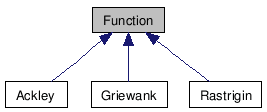
\includegraphics[width=118pt]{classFunction__inherit__graph}
\end{center}
\end{figure}
\subsection*{Public Member Functions}
\begin{CompactItemize}
\item 
virtual double \hyperlink{classFunction_9323a7309b16e0e168590e34b359ff32}{evaluate} (vector$<$ double $>$ \&x)=0
\end{CompactItemize}
\subsection*{Public Attributes}
\begin{CompactItemize}
\item 
int \hyperlink{classFunction_2f582d2da9cb2af5507a55e17bc44083}{n}
\item 
vector$<$ pair$<$ double, double $>$ $>$ \hyperlink{classFunction_e846ed04f4211984a2162b620ee91c81}{constraint}
\end{CompactItemize}


\subsection{Member Function Documentation}
\hypertarget{classFunction_9323a7309b16e0e168590e34b359ff32}{
\index{Function@{Function}!evaluate@{evaluate}}
\index{evaluate@{evaluate}!Function@{Function}}
\subsubsection{\setlength{\rightskip}{0pt plus 5cm}virtual double Function::evaluate (vector$<$ double $>$ \& {\em x})\hspace{0.3cm}{\tt  \mbox{[}pure virtual\mbox{]}}}}
\label{classFunction_9323a7309b16e0e168590e34b359ff32}




Implemented in \hyperlink{classGriewank_c34b1c32bfb7b867c6772db5cc6a727f}{Griewank}, \hyperlink{classAckley_6423fcd54b72322f08357879bac580b6}{Ackley}, and \hyperlink{classRastrigin_aba8c37ab1546da6e7ed47123d179673}{Rastrigin}.

\subsection{Member Data Documentation}
\hypertarget{classFunction_2f582d2da9cb2af5507a55e17bc44083}{
\index{Function@{Function}!n@{n}}
\index{n@{n}!Function@{Function}}
\subsubsection{\setlength{\rightskip}{0pt plus 5cm}int {\bf Function::n}}}
\label{classFunction_2f582d2da9cb2af5507a55e17bc44083}


dimension \hypertarget{classFunction_e846ed04f4211984a2162b620ee91c81}{
\index{Function@{Function}!constraint@{constraint}}
\index{constraint@{constraint}!Function@{Function}}
\subsubsection{\setlength{\rightskip}{0pt plus 5cm}vector$<$pair$<$double, double$>$ $>$ {\bf Function::constraint}}}
\label{classFunction_e846ed04f4211984a2162b620ee91c81}




The documentation for this class was generated from the following file:\begin{CompactItemize}
\item 
\hyperlink{Functions_8h}{Functions.h}\end{CompactItemize}

\hypertarget{classpso_1_1Function}{
\section{pso::Function Class Reference}
\label{classpso_1_1Function}\index{pso::Function@{pso::Function}}
}
Inheritance diagram for pso::Function:Collaboration diagram for pso::Function:\subsection*{Public Member Functions}
\begin{CompactItemize}
\item 
def \hyperlink{classpso_1_1Function_959f07a6de4f333461fdb0261e6c25ae}{\_\-\_\-repr\_\-\_\-}
\item 
def \hyperlink{classpso_1_1Function_6874097c6476dc85af64b40e76a807e9}{\_\-\_\-init\_\-\_\-}
\item 
def \hyperlink{classpso_1_1Function_c80bd40fcf4a956e5732ed099bccc598}{\_\-\_\-del\_\-\_\-}
\item 
def \hyperlink{classpso_1_1Function_7c958ea6d942a89ae219b872b4d73541}{evaluate}
\item 
def \hyperlink{classpso_1_1Function_519ce59a07719b4a0bea88a642e1c685}{noisyEvaluate}
\item 
def \hyperlink{classpso_1_1Function_b513ffe2a27e5f3ff68f40bd20680825}{addNoisePos}
\item 
def \hyperlink{classpso_1_1Function_fe29a56e75f3a076e00fdecbb8d4197d}{addNoiseVal}
\item 
def \hyperlink{classpso_1_1Function_839d1e649623a32eef82be4e64f481ad}{addNoiseRelativeVal}
\item 
def \hyperlink{classpso_1_1Function_95ef0ee896d9855495cb2518c368fecf}{update}
\item 
def \hyperlink{classpso_1_1Function_f9adcf9d0da73d89e6f411f0f0f27d2c}{getGoal}
\item 
def \hyperlink{classpso_1_1Function_ec3f76a1844cf52fd7a4f49856e6a40e}{getOpt}
\item 
def \hyperlink{classpso_1_1Function_b502339a9dc9eaed402856156b8f0932}{get\_\-min\_\-x}
\item 
def \hyperlink{classpso_1_1Function_fb6726a96d5ab4dcb6ac845a95172585}{get\_\-max\_\-x}
\item 
def \hyperlink{classpso_1_1Function_6d2c5e6dca8a99d077e0a1679c7e3a14}{get\_\-min\_\-v}
\item 
def \hyperlink{classpso_1_1Function_0de152ecef2a4263ec72fa949540efed}{get\_\-max\_\-v}
\item 
def \hyperlink{classpso_1_1Function_d1fbe76a7087621326b7bc1c29076704}{setNoiseStyle}
\item 
def \hyperlink{classpso_1_1Function_b42bbaac0bf52ef8b09b92d29f23e37b}{setNoiseSigma}
\item 
def \hyperlink{classpso_1_1Function_a6d712e3ddbea4eb72e83d40f51b8b4c}{getNoiseStyle}
\item 
def \hyperlink{classpso_1_1Function_5f7b9b3753e6501d12711d74234bb6ac}{getNoiseSigma}
\item 
def \hyperlink{classpso_1_1Function_bcbf334641bdedf80d15c08505951db8}{getDynamicStyle}
\item 
def \hyperlink{classpso_1_1Function_f986351a95b4937d390fa6803e7a845b}{getOptPosition}
\item 
def \hyperlink{classpso_1_1Function_76aee0acd25d5a9b207a307369b80f1b}{set\_\-moveFrequency}
\item 
def \hyperlink{classpso_1_1Function_2376cbe3a5701668c87049794b47b0db}{set\_\-moveDistance}
\item 
def \hyperlink{classpso_1_1Function_1a6dbfccf99208be62712a999eb041b9}{set\_\-optMoveStyle}
\item 
def \hyperlink{classpso_1_1Function_881d3f6532171a36f736edf783c6b10b}{set\_\-updateStyle}
\item 
def \hyperlink{classpso_1_1Function_c9d5dace0aa15c12eff310496a978ad5}{get\_\-moveFrequency}
\item 
def \hyperlink{classpso_1_1Function_03d8ad4749da59e8031e18d4bddff6c4}{get\_\-moveDistance}
\item 
def \hyperlink{classpso_1_1Function_f70f31465c6e4464cafbe2710352e18b}{get\_\-optMoveStyle}
\item 
def \hyperlink{classpso_1_1Function_f09d4d5ef25e3158fed9d0255a5a5748}{get\_\-updateStyle}
\end{CompactItemize}
\subsection*{Static Private Attributes}
\begin{CompactItemize}
\item 
dictionary \hyperlink{classpso_1_1Function_2334bfe507115d58047f67960dde71d3}{\_\-\_\-swig\_\-setmethods\_\-\_\-} = \{\}
\item 
tuple \hyperlink{classpso_1_1Function_cd8775cf6aadc3fdf4e6d82158ef10fb}{\_\-\_\-setattr\_\-\_\-} = lambdaself,name,value:\_\-swig\_\-setattr(self, \hyperlink{classpso_1_1Function}{Function}, name, value)
\item 
dictionary \hyperlink{classpso_1_1Function_5bddc07dbaab0ee579488bdcc8103a71}{\_\-\_\-swig\_\-getmethods\_\-\_\-} = \{\}
\item 
tuple \hyperlink{classpso_1_1Function_affeed856b337656e88895fa35321496}{\_\-\_\-getattr\_\-\_\-} = lambdaself,name:\_\-swig\_\-getattr(self, \hyperlink{classpso_1_1Function}{Function}, name)
\end{CompactItemize}


\subsection{Member Function Documentation}
\hypertarget{classpso_1_1Function_959f07a6de4f333461fdb0261e6c25ae}{
\index{pso::Function@{pso::Function}!\_\-\_\-repr\_\-\_\-@{\_\-\_\-repr\_\-\_\-}}
\index{\_\-\_\-repr\_\-\_\-@{\_\-\_\-repr\_\-\_\-}!pso::Function@{pso::Function}}
\subsubsection{\setlength{\rightskip}{0pt plus 5cm}def pso::Function::\_\-\_\-repr\_\-\_\- ( {\em self})}}
\label{classpso_1_1Function_959f07a6de4f333461fdb0261e6c25ae}




Reimplemented in \hyperlink{classpso_1_1Sphere_97873feed050d378f3f3a83340619732}{pso::Sphere}, \hyperlink{classpso_1_1Rosenbrock_56aac438a1d2c22a725967ecef381344}{pso::Rosenbrock}, \hyperlink{classpso_1_1Rastrigin_e20e3e7a699b801c9fa78b531ae355c1}{pso::Rastrigin}, \hyperlink{classpso_1_1Schaffer_8b59b8cfafafad160fa0deac772d0191}{pso::Schaffer}, \hyperlink{classpso_1_1Griewank_511aaa7b5b0c146773011fc3d889e43f}{pso::Griewank}, \hyperlink{classpso_1_1Ackley_e8ad324464b4641ea1b71ba20d3fe12c}{pso::Ackley}, \hyperlink{classpso_1_1Schwefel_355d3604b3f13580871f2eeb90d42ef4}{pso::Schwefel}, \hyperlink{classpso_1_1Levy5_b10ee4210aa6d53ec66a9c79e6558e20}{pso::Levy5}, \hyperlink{classpso_1_1Freudenstein_593b2ae91d886ecccd01877ac2321ae4}{pso::Freudenstein}, \hyperlink{classpso_1_1Quadric_c345dddcc2571f2daaf90a6ba9dcc237}{pso::Quadric}, \hyperlink{classpso_1_1MovingGoal_9a7bc1af4d07be74f83fda41d598ef9b}{pso::MovingGoal}, \hyperlink{classpso_1_1MovingPeaks_a49761a17dfa13ee9bd3854cae9b6db7}{pso::MovingPeaks}, and \hyperlink{classpso_1_1Sinusoidal_b6343711af3f82150f169132f230fd80}{pso::Sinusoidal}.\hypertarget{classpso_1_1Function_6874097c6476dc85af64b40e76a807e9}{
\index{pso::Function@{pso::Function}!\_\-\_\-init\_\-\_\-@{\_\-\_\-init\_\-\_\-}}
\index{\_\-\_\-init\_\-\_\-@{\_\-\_\-init\_\-\_\-}!pso::Function@{pso::Function}}
\subsubsection{\setlength{\rightskip}{0pt plus 5cm}def pso::Function::\_\-\_\-init\_\-\_\- ( {\em self}, \/   {\em args})}}
\label{classpso_1_1Function_6874097c6476dc85af64b40e76a807e9}




Reimplemented in \hyperlink{classpso_1_1FunctionPtr_5370977bbb543767eef37e2dab6e49b9}{pso::FunctionPtr}, \hyperlink{classpso_1_1Sphere_e4b014b1b87400b7a6a35b5f2311620a}{pso::Sphere}, \hyperlink{classpso_1_1SpherePtr_5ce4f7ba2467b0c1a36992cbe1bd7e4d}{pso::SpherePtr}, \hyperlink{classpso_1_1Rosenbrock_10f77ae0f5c18274477e3102632b24f1}{pso::Rosenbrock}, \hyperlink{classpso_1_1RosenbrockPtr_cd5936c5a86eae090b9b9d473e6fa87c}{pso::RosenbrockPtr}, \hyperlink{classpso_1_1Rastrigin_6a38343c1d2870431835ecb1a82d43b2}{pso::Rastrigin}, \hyperlink{classpso_1_1RastriginPtr_e68fff937daab154626622e257267a58}{pso::RastriginPtr}, \hyperlink{classpso_1_1Schaffer_ff9f1ae937ff0d73aeb17bb27be9b5f3}{pso::Schaffer}, \hyperlink{classpso_1_1SchafferPtr_ed11725f1cd7627f537b7daad5560125}{pso::SchafferPtr}, \hyperlink{classpso_1_1Griewank_c84ac13db6c58cd5ca948ba0340ab4f8}{pso::Griewank}, \hyperlink{classpso_1_1GriewankPtr_0814eb7cbb6badaa00a5eeb06077b7db}{pso::GriewankPtr}, \hyperlink{classpso_1_1Ackley_df19f3468a7b5b260adffcd134145e24}{pso::Ackley}, \hyperlink{classpso_1_1AckleyPtr_92267323798f30fea8a7d1e807261dc3}{pso::AckleyPtr}, \hyperlink{classpso_1_1Schwefel_923da07160f0471b0797a092dc53f05f}{pso::Schwefel}, \hyperlink{classpso_1_1SchwefelPtr_073a6a9bb2a9778745ac521f508634a0}{pso::SchwefelPtr}, \hyperlink{classpso_1_1Levy5_3499ee5a0ad4b26fb90f4aeb8b899585}{pso::Levy5}, \hyperlink{classpso_1_1Levy5Ptr_01f10ada921645bf0be74d8073c0c764}{pso::Levy5Ptr}, \hyperlink{classpso_1_1Freudenstein_5bede09ddc059943e97451908bf5b622}{pso::Freudenstein}, \hyperlink{classpso_1_1FreudensteinPtr_605822702b355b32a6ca939c0aae1656}{pso::FreudensteinPtr}, \hyperlink{classpso_1_1Quadric_fed66f973031f5c183bbdb8ac437315c}{pso::Quadric}, \hyperlink{classpso_1_1QuadricPtr_206857d4cf8c3ad6fad721d0ef9fc966}{pso::QuadricPtr}, \hyperlink{classpso_1_1MovingGoal_cc887e0a1449493e7497703a3c6633f3}{pso::MovingGoal}, \hyperlink{classpso_1_1MovingGoalPtr_b48d8f3578706bbddfb9110c88acc239}{pso::MovingGoalPtr}, \hyperlink{classpso_1_1MovingPeaks_f48b3a4fe44b6a14626ea7c9dfaccd66}{pso::MovingPeaks}, \hyperlink{classpso_1_1MovingPeaksPtr_32e785c6b0bffba8a0baee3920aa31eb}{pso::MovingPeaksPtr}, \hyperlink{classpso_1_1Sinusoidal_a75df3138290d6798a97d2ffe7b1c68b}{pso::Sinusoidal}, and \hyperlink{classpso_1_1SinusoidalPtr_086a4ea046d5a57f475e3e37952d976a}{pso::SinusoidalPtr}.\hypertarget{classpso_1_1Function_c80bd40fcf4a956e5732ed099bccc598}{
\index{pso::Function@{pso::Function}!\_\-\_\-del\_\-\_\-@{\_\-\_\-del\_\-\_\-}}
\index{\_\-\_\-del\_\-\_\-@{\_\-\_\-del\_\-\_\-}!pso::Function@{pso::Function}}
\subsubsection{\setlength{\rightskip}{0pt plus 5cm}def pso::Function::\_\-\_\-del\_\-\_\- ( {\em self}, \/   {\em destroy} = {\tt \_\-pso.delete\_\-Function})}}
\label{classpso_1_1Function_c80bd40fcf4a956e5732ed099bccc598}




Reimplemented in \hyperlink{classpso_1_1Sphere_71a5156269bbb4a9ccc41410990e5dcb}{pso::Sphere}, \hyperlink{classpso_1_1Rosenbrock_424c4c5cda5831c268442b97ea667618}{pso::Rosenbrock}, \hyperlink{classpso_1_1Rastrigin_4ec1ea0cb3ef15cb5355eb5b36cfeabf}{pso::Rastrigin}, \hyperlink{classpso_1_1Schaffer_a8c2032038b61e7a1f61f45ba0f86ccd}{pso::Schaffer}, \hyperlink{classpso_1_1Griewank_de940e1ba1459422e6e012a71a09f14b}{pso::Griewank}, \hyperlink{classpso_1_1Ackley_60113ede99369f390dc78a45e625342c}{pso::Ackley}, \hyperlink{classpso_1_1Schwefel_934aebcd5b45f4fda0b97076b4db949c}{pso::Schwefel}, \hyperlink{classpso_1_1Levy5_b19922a937c1d22b02f24853a96bf271}{pso::Levy5}, \hyperlink{classpso_1_1Freudenstein_bcb8a7755b12ba21aa67353f25b4b243}{pso::Freudenstein}, \hyperlink{classpso_1_1Quadric_643ec4862385919c0e08f61f356ea0e6}{pso::Quadric}, \hyperlink{classpso_1_1MovingGoal_ccd203604cd67870527b7b16d0be7564}{pso::MovingGoal}, \hyperlink{classpso_1_1MovingPeaks_51bfd4ae5fc9d7b2f6ed4ebcc8f3470b}{pso::MovingPeaks}, and \hyperlink{classpso_1_1Sinusoidal_8b3ba4783d55a0536cfde0c74c1a8e6e}{pso::Sinusoidal}.\hypertarget{classpso_1_1Function_7c958ea6d942a89ae219b872b4d73541}{
\index{pso::Function@{pso::Function}!evaluate@{evaluate}}
\index{evaluate@{evaluate}!pso::Function@{pso::Function}}
\subsubsection{\setlength{\rightskip}{0pt plus 5cm}def pso::Function::evaluate ( {\em args})}}
\label{classpso_1_1Function_7c958ea6d942a89ae219b872b4d73541}




Reimplemented in \hyperlink{classpso_1_1Sphere_2c17788061780a2050cebccfec6a49c7}{pso::Sphere}, \hyperlink{classpso_1_1Rosenbrock_8609c7b4f2ca951920cfee0cb6fdacc4}{pso::Rosenbrock}, \hyperlink{classpso_1_1Rastrigin_6aaed0f64f959a9666321763e3ff8efe}{pso::Rastrigin}, \hyperlink{classpso_1_1Schaffer_575dd83cea9a359e9233918331ef4ada}{pso::Schaffer}, \hyperlink{classpso_1_1Griewank_13250cfc11071d8fd3bf65a5eb69f397}{pso::Griewank}, \hyperlink{classpso_1_1Ackley_bf28e608baadcbc4a9795993584f985b}{pso::Ackley}, \hyperlink{classpso_1_1Schwefel_ffe14ee462d46bf76e19065c755bb013}{pso::Schwefel}, \hyperlink{classpso_1_1Levy5_7de80ec535099658cfc10dac658aaf4e}{pso::Levy5}, \hyperlink{classpso_1_1Freudenstein_bfe2aea7372da1083a9f562ec6c4ed82}{pso::Freudenstein}, \hyperlink{classpso_1_1Quadric_bf922b6bbf00b01ca2a449078ecff65a}{pso::Quadric}, \hyperlink{classpso_1_1MovingGoal_16ffa8c492ff6f56ed8fcbf20f168bdd}{pso::MovingGoal}, \hyperlink{classpso_1_1MovingPeaks_bac0595181eff4c3e7b1975e58c7af22}{pso::MovingPeaks}, and \hyperlink{classpso_1_1Sinusoidal_4c9e94b27d920bbee7cb3fc8ac4c09c7}{pso::Sinusoidal}.\hypertarget{classpso_1_1Function_519ce59a07719b4a0bea88a642e1c685}{
\index{pso::Function@{pso::Function}!noisyEvaluate@{noisyEvaluate}}
\index{noisyEvaluate@{noisyEvaluate}!pso::Function@{pso::Function}}
\subsubsection{\setlength{\rightskip}{0pt plus 5cm}def pso::Function::noisyEvaluate ( {\em args})}}
\label{classpso_1_1Function_519ce59a07719b4a0bea88a642e1c685}


\hypertarget{classpso_1_1Function_b513ffe2a27e5f3ff68f40bd20680825}{
\index{pso::Function@{pso::Function}!addNoisePos@{addNoisePos}}
\index{addNoisePos@{addNoisePos}!pso::Function@{pso::Function}}
\subsubsection{\setlength{\rightskip}{0pt plus 5cm}def pso::Function::addNoisePos ( {\em args})}}
\label{classpso_1_1Function_b513ffe2a27e5f3ff68f40bd20680825}


\hypertarget{classpso_1_1Function_fe29a56e75f3a076e00fdecbb8d4197d}{
\index{pso::Function@{pso::Function}!addNoiseVal@{addNoiseVal}}
\index{addNoiseVal@{addNoiseVal}!pso::Function@{pso::Function}}
\subsubsection{\setlength{\rightskip}{0pt plus 5cm}def pso::Function::addNoiseVal ( {\em args})}}
\label{classpso_1_1Function_fe29a56e75f3a076e00fdecbb8d4197d}


\hypertarget{classpso_1_1Function_839d1e649623a32eef82be4e64f481ad}{
\index{pso::Function@{pso::Function}!addNoiseRelativeVal@{addNoiseRelativeVal}}
\index{addNoiseRelativeVal@{addNoiseRelativeVal}!pso::Function@{pso::Function}}
\subsubsection{\setlength{\rightskip}{0pt plus 5cm}def pso::Function::addNoiseRelativeVal ( {\em args})}}
\label{classpso_1_1Function_839d1e649623a32eef82be4e64f481ad}


\hypertarget{classpso_1_1Function_95ef0ee896d9855495cb2518c368fecf}{
\index{pso::Function@{pso::Function}!update@{update}}
\index{update@{update}!pso::Function@{pso::Function}}
\subsubsection{\setlength{\rightskip}{0pt plus 5cm}def pso::Function::update ( {\em args})}}
\label{classpso_1_1Function_95ef0ee896d9855495cb2518c368fecf}




Reimplemented in \hyperlink{classpso_1_1MovingPeaks_2498bfb3e35cc34ed63f1fcf6c8dbdd6}{pso::MovingPeaks}, and \hyperlink{classpso_1_1Sinusoidal_56ebee67a884bc171cddea452bf12f2e}{pso::Sinusoidal}.\hypertarget{classpso_1_1Function_f9adcf9d0da73d89e6f411f0f0f27d2c}{
\index{pso::Function@{pso::Function}!getGoal@{getGoal}}
\index{getGoal@{getGoal}!pso::Function@{pso::Function}}
\subsubsection{\setlength{\rightskip}{0pt plus 5cm}def pso::Function::getGoal ( {\em args})}}
\label{classpso_1_1Function_f9adcf9d0da73d89e6f411f0f0f27d2c}


\hypertarget{classpso_1_1Function_ec3f76a1844cf52fd7a4f49856e6a40e}{
\index{pso::Function@{pso::Function}!getOpt@{getOpt}}
\index{getOpt@{getOpt}!pso::Function@{pso::Function}}
\subsubsection{\setlength{\rightskip}{0pt plus 5cm}def pso::Function::getOpt ( {\em args})}}
\label{classpso_1_1Function_ec3f76a1844cf52fd7a4f49856e6a40e}


\hypertarget{classpso_1_1Function_b502339a9dc9eaed402856156b8f0932}{
\index{pso::Function@{pso::Function}!get\_\-min\_\-x@{get\_\-min\_\-x}}
\index{get\_\-min\_\-x@{get\_\-min\_\-x}!pso::Function@{pso::Function}}
\subsubsection{\setlength{\rightskip}{0pt plus 5cm}def pso::Function::get\_\-min\_\-x ( {\em args})}}
\label{classpso_1_1Function_b502339a9dc9eaed402856156b8f0932}


\hypertarget{classpso_1_1Function_fb6726a96d5ab4dcb6ac845a95172585}{
\index{pso::Function@{pso::Function}!get\_\-max\_\-x@{get\_\-max\_\-x}}
\index{get\_\-max\_\-x@{get\_\-max\_\-x}!pso::Function@{pso::Function}}
\subsubsection{\setlength{\rightskip}{0pt plus 5cm}def pso::Function::get\_\-max\_\-x ( {\em args})}}
\label{classpso_1_1Function_fb6726a96d5ab4dcb6ac845a95172585}


\hypertarget{classpso_1_1Function_6d2c5e6dca8a99d077e0a1679c7e3a14}{
\index{pso::Function@{pso::Function}!get\_\-min\_\-v@{get\_\-min\_\-v}}
\index{get\_\-min\_\-v@{get\_\-min\_\-v}!pso::Function@{pso::Function}}
\subsubsection{\setlength{\rightskip}{0pt plus 5cm}def pso::Function::get\_\-min\_\-v ( {\em args})}}
\label{classpso_1_1Function_6d2c5e6dca8a99d077e0a1679c7e3a14}


\hypertarget{classpso_1_1Function_0de152ecef2a4263ec72fa949540efed}{
\index{pso::Function@{pso::Function}!get\_\-max\_\-v@{get\_\-max\_\-v}}
\index{get\_\-max\_\-v@{get\_\-max\_\-v}!pso::Function@{pso::Function}}
\subsubsection{\setlength{\rightskip}{0pt plus 5cm}def pso::Function::get\_\-max\_\-v ( {\em args})}}
\label{classpso_1_1Function_0de152ecef2a4263ec72fa949540efed}


\hypertarget{classpso_1_1Function_d1fbe76a7087621326b7bc1c29076704}{
\index{pso::Function@{pso::Function}!setNoiseStyle@{setNoiseStyle}}
\index{setNoiseStyle@{setNoiseStyle}!pso::Function@{pso::Function}}
\subsubsection{\setlength{\rightskip}{0pt plus 5cm}def pso::Function::setNoiseStyle ( {\em args})}}
\label{classpso_1_1Function_d1fbe76a7087621326b7bc1c29076704}


\hypertarget{classpso_1_1Function_b42bbaac0bf52ef8b09b92d29f23e37b}{
\index{pso::Function@{pso::Function}!setNoiseSigma@{setNoiseSigma}}
\index{setNoiseSigma@{setNoiseSigma}!pso::Function@{pso::Function}}
\subsubsection{\setlength{\rightskip}{0pt plus 5cm}def pso::Function::setNoiseSigma ( {\em args})}}
\label{classpso_1_1Function_b42bbaac0bf52ef8b09b92d29f23e37b}


\hypertarget{classpso_1_1Function_a6d712e3ddbea4eb72e83d40f51b8b4c}{
\index{pso::Function@{pso::Function}!getNoiseStyle@{getNoiseStyle}}
\index{getNoiseStyle@{getNoiseStyle}!pso::Function@{pso::Function}}
\subsubsection{\setlength{\rightskip}{0pt plus 5cm}def pso::Function::getNoiseStyle ( {\em args})}}
\label{classpso_1_1Function_a6d712e3ddbea4eb72e83d40f51b8b4c}


\hypertarget{classpso_1_1Function_5f7b9b3753e6501d12711d74234bb6ac}{
\index{pso::Function@{pso::Function}!getNoiseSigma@{getNoiseSigma}}
\index{getNoiseSigma@{getNoiseSigma}!pso::Function@{pso::Function}}
\subsubsection{\setlength{\rightskip}{0pt plus 5cm}def pso::Function::getNoiseSigma ( {\em args})}}
\label{classpso_1_1Function_5f7b9b3753e6501d12711d74234bb6ac}


\hypertarget{classpso_1_1Function_bcbf334641bdedf80d15c08505951db8}{
\index{pso::Function@{pso::Function}!getDynamicStyle@{getDynamicStyle}}
\index{getDynamicStyle@{getDynamicStyle}!pso::Function@{pso::Function}}
\subsubsection{\setlength{\rightskip}{0pt plus 5cm}def pso::Function::getDynamicStyle ( {\em args})}}
\label{classpso_1_1Function_bcbf334641bdedf80d15c08505951db8}


\hypertarget{classpso_1_1Function_f986351a95b4937d390fa6803e7a845b}{
\index{pso::Function@{pso::Function}!getOptPosition@{getOptPosition}}
\index{getOptPosition@{getOptPosition}!pso::Function@{pso::Function}}
\subsubsection{\setlength{\rightskip}{0pt plus 5cm}def pso::Function::getOptPosition ( {\em args})}}
\label{classpso_1_1Function_f986351a95b4937d390fa6803e7a845b}


\hypertarget{classpso_1_1Function_76aee0acd25d5a9b207a307369b80f1b}{
\index{pso::Function@{pso::Function}!set\_\-moveFrequency@{set\_\-moveFrequency}}
\index{set\_\-moveFrequency@{set\_\-moveFrequency}!pso::Function@{pso::Function}}
\subsubsection{\setlength{\rightskip}{0pt plus 5cm}def pso::Function::set\_\-moveFrequency ( {\em args})}}
\label{classpso_1_1Function_76aee0acd25d5a9b207a307369b80f1b}


\hypertarget{classpso_1_1Function_2376cbe3a5701668c87049794b47b0db}{
\index{pso::Function@{pso::Function}!set\_\-moveDistance@{set\_\-moveDistance}}
\index{set\_\-moveDistance@{set\_\-moveDistance}!pso::Function@{pso::Function}}
\subsubsection{\setlength{\rightskip}{0pt plus 5cm}def pso::Function::set\_\-moveDistance ( {\em args})}}
\label{classpso_1_1Function_2376cbe3a5701668c87049794b47b0db}




Reimplemented in \hyperlink{classpso_1_1MovingPeaks_5ade0db216cabe9a9eb062e7dcc59ec2}{pso::MovingPeaks}.\hypertarget{classpso_1_1Function_1a6dbfccf99208be62712a999eb041b9}{
\index{pso::Function@{pso::Function}!set\_\-optMoveStyle@{set\_\-optMoveStyle}}
\index{set\_\-optMoveStyle@{set\_\-optMoveStyle}!pso::Function@{pso::Function}}
\subsubsection{\setlength{\rightskip}{0pt plus 5cm}def pso::Function::set\_\-optMoveStyle ( {\em args})}}
\label{classpso_1_1Function_1a6dbfccf99208be62712a999eb041b9}


\hypertarget{classpso_1_1Function_881d3f6532171a36f736edf783c6b10b}{
\index{pso::Function@{pso::Function}!set\_\-updateStyle@{set\_\-updateStyle}}
\index{set\_\-updateStyle@{set\_\-updateStyle}!pso::Function@{pso::Function}}
\subsubsection{\setlength{\rightskip}{0pt plus 5cm}def pso::Function::set\_\-updateStyle ( {\em args})}}
\label{classpso_1_1Function_881d3f6532171a36f736edf783c6b10b}


\hypertarget{classpso_1_1Function_c9d5dace0aa15c12eff310496a978ad5}{
\index{pso::Function@{pso::Function}!get\_\-moveFrequency@{get\_\-moveFrequency}}
\index{get\_\-moveFrequency@{get\_\-moveFrequency}!pso::Function@{pso::Function}}
\subsubsection{\setlength{\rightskip}{0pt plus 5cm}def pso::Function::get\_\-moveFrequency ( {\em args})}}
\label{classpso_1_1Function_c9d5dace0aa15c12eff310496a978ad5}


\hypertarget{classpso_1_1Function_03d8ad4749da59e8031e18d4bddff6c4}{
\index{pso::Function@{pso::Function}!get\_\-moveDistance@{get\_\-moveDistance}}
\index{get\_\-moveDistance@{get\_\-moveDistance}!pso::Function@{pso::Function}}
\subsubsection{\setlength{\rightskip}{0pt plus 5cm}def pso::Function::get\_\-moveDistance ( {\em args})}}
\label{classpso_1_1Function_03d8ad4749da59e8031e18d4bddff6c4}


\hypertarget{classpso_1_1Function_f70f31465c6e4464cafbe2710352e18b}{
\index{pso::Function@{pso::Function}!get\_\-optMoveStyle@{get\_\-optMoveStyle}}
\index{get\_\-optMoveStyle@{get\_\-optMoveStyle}!pso::Function@{pso::Function}}
\subsubsection{\setlength{\rightskip}{0pt plus 5cm}def pso::Function::get\_\-optMoveStyle ( {\em args})}}
\label{classpso_1_1Function_f70f31465c6e4464cafbe2710352e18b}


\hypertarget{classpso_1_1Function_f09d4d5ef25e3158fed9d0255a5a5748}{
\index{pso::Function@{pso::Function}!get\_\-updateStyle@{get\_\-updateStyle}}
\index{get\_\-updateStyle@{get\_\-updateStyle}!pso::Function@{pso::Function}}
\subsubsection{\setlength{\rightskip}{0pt plus 5cm}def pso::Function::get\_\-updateStyle ( {\em args})}}
\label{classpso_1_1Function_f09d4d5ef25e3158fed9d0255a5a5748}




\subsection{Field Documentation}
\hypertarget{classpso_1_1Function_2334bfe507115d58047f67960dde71d3}{
\index{pso::Function@{pso::Function}!\_\-\_\-swig\_\-setmethods\_\-\_\-@{\_\-\_\-swig\_\-setmethods\_\-\_\-}}
\index{\_\-\_\-swig\_\-setmethods\_\-\_\-@{\_\-\_\-swig\_\-setmethods\_\-\_\-}!pso::Function@{pso::Function}}
\subsubsection{\setlength{\rightskip}{0pt plus 5cm}dictionary {\bf pso::Function::\_\-\_\-swig\_\-setmethods\_\-\_\-} = \{\}\hspace{0.3cm}{\tt  \mbox{[}static, private\mbox{]}}}}
\label{classpso_1_1Function_2334bfe507115d58047f67960dde71d3}




Reimplemented in \hyperlink{classpso_1_1Sphere_9c2b9a1bd59f55c2010cbceda68c5916}{pso::Sphere}, \hyperlink{classpso_1_1Rosenbrock_7b19f06e4baa11a3daf3c6faccdb7241}{pso::Rosenbrock}, \hyperlink{classpso_1_1Rastrigin_6669f18ee53e453abd57a7414869091c}{pso::Rastrigin}, \hyperlink{classpso_1_1Schaffer_b037f1ad69b6619f1f89c7ba8e5de505}{pso::Schaffer}, \hyperlink{classpso_1_1Griewank_9d6ac056840192478ec5f46980eb1231}{pso::Griewank}, \hyperlink{classpso_1_1Ackley_8b601c932da42d58672496d0b982e333}{pso::Ackley}, \hyperlink{classpso_1_1Schwefel_c3b3a6c2afe3fd3d83656d02402cad2e}{pso::Schwefel}, \hyperlink{classpso_1_1Levy5_93d6c8d420b6ad862c41073e1764d31e}{pso::Levy5}, \hyperlink{classpso_1_1Freudenstein_d9e773221878926aafbb38d695a4017e}{pso::Freudenstein}, \hyperlink{classpso_1_1Quadric_5953ccca68eb821e48ff2953838604b7}{pso::Quadric}, \hyperlink{classpso_1_1MovingGoal_ec7da72a4fcf6a13f9f700b4dcf02b34}{pso::MovingGoal}, \hyperlink{classpso_1_1MovingPeaks_635671a6ae57a2c5d14d2ab1627f2f2c}{pso::MovingPeaks}, and \hyperlink{classpso_1_1Sinusoidal_7bdd3d830dd4d4cbe4481f4ac2f2db41}{pso::Sinusoidal}.\hypertarget{classpso_1_1Function_cd8775cf6aadc3fdf4e6d82158ef10fb}{
\index{pso::Function@{pso::Function}!\_\-\_\-setattr\_\-\_\-@{\_\-\_\-setattr\_\-\_\-}}
\index{\_\-\_\-setattr\_\-\_\-@{\_\-\_\-setattr\_\-\_\-}!pso::Function@{pso::Function}}
\subsubsection{\setlength{\rightskip}{0pt plus 5cm}tuple {\bf pso::Function::\_\-\_\-setattr\_\-\_\-} = lambdaself,name,value:\_\-swig\_\-setattr(self, {\bf Function}, name, value)\hspace{0.3cm}{\tt  \mbox{[}static, private\mbox{]}}}}
\label{classpso_1_1Function_cd8775cf6aadc3fdf4e6d82158ef10fb}




Reimplemented in \hyperlink{classpso_1_1Sphere_303c4331c24184d721f1284e405b7453}{pso::Sphere}, \hyperlink{classpso_1_1Rosenbrock_20daa93c52410a96f8e6affaaed83d36}{pso::Rosenbrock}, \hyperlink{classpso_1_1Rastrigin_cf1c6ea103beabbdb11abbd8a0e6d1fc}{pso::Rastrigin}, \hyperlink{classpso_1_1Schaffer_15fbb90f609e96f5533449e989908d5d}{pso::Schaffer}, \hyperlink{classpso_1_1Griewank_bf26d6b7263a0aa9ebc00059a5cda5cc}{pso::Griewank}, \hyperlink{classpso_1_1Ackley_b19008786aca804a23b7fa7744c89c25}{pso::Ackley}, \hyperlink{classpso_1_1Schwefel_cf6df02d5b7d6b9dc27ea126a521c53d}{pso::Schwefel}, \hyperlink{classpso_1_1Levy5_4460b9b9e78befc1daa52a2cedfb6178}{pso::Levy5}, \hyperlink{classpso_1_1Freudenstein_13d26a6411b620f14698a539a7321080}{pso::Freudenstein}, \hyperlink{classpso_1_1Quadric_39d18c5e187c40c760304ac789fd813c}{pso::Quadric}, \hyperlink{classpso_1_1MovingGoal_bfa092e032ac4ccf2c8d070ec1e33dab}{pso::MovingGoal}, \hyperlink{classpso_1_1MovingPeaks_a30c9de8ca26c42218b1c3a211f7d0cf}{pso::MovingPeaks}, and \hyperlink{classpso_1_1Sinusoidal_102c00e25a425a175159522a597af525}{pso::Sinusoidal}.\hypertarget{classpso_1_1Function_5bddc07dbaab0ee579488bdcc8103a71}{
\index{pso::Function@{pso::Function}!\_\-\_\-swig\_\-getmethods\_\-\_\-@{\_\-\_\-swig\_\-getmethods\_\-\_\-}}
\index{\_\-\_\-swig\_\-getmethods\_\-\_\-@{\_\-\_\-swig\_\-getmethods\_\-\_\-}!pso::Function@{pso::Function}}
\subsubsection{\setlength{\rightskip}{0pt plus 5cm}dictionary {\bf pso::Function::\_\-\_\-swig\_\-getmethods\_\-\_\-} = \{\}\hspace{0.3cm}{\tt  \mbox{[}static, private\mbox{]}}}}
\label{classpso_1_1Function_5bddc07dbaab0ee579488bdcc8103a71}




Reimplemented in \hyperlink{classpso_1_1Sphere_0c0cc3d04e98d1dc9576e1bdf5fa34ed}{pso::Sphere}, \hyperlink{classpso_1_1Rosenbrock_5228ee78176ce890dca261f8e0b5b20a}{pso::Rosenbrock}, \hyperlink{classpso_1_1Rastrigin_ff2a6f19b803ab401dc52374ea84bf27}{pso::Rastrigin}, \hyperlink{classpso_1_1Schaffer_3017db451e46ba369ce62cc2b7ee6dba}{pso::Schaffer}, \hyperlink{classpso_1_1Griewank_df761ea1e5152ee4b7aec7de9f3b86c3}{pso::Griewank}, \hyperlink{classpso_1_1Ackley_48bbde97c1ea3bf426dceed5fa9ca874}{pso::Ackley}, \hyperlink{classpso_1_1Schwefel_069965b80402f68af7a664aea8aea22f}{pso::Schwefel}, \hyperlink{classpso_1_1Levy5_2bd3aa2316c11de1d2c76347089ec9fb}{pso::Levy5}, \hyperlink{classpso_1_1Freudenstein_5e01e784238005f1fe1d4befa249be0f}{pso::Freudenstein}, \hyperlink{classpso_1_1Quadric_d98a08d9dc318dfb0799dc8a0f442370}{pso::Quadric}, \hyperlink{classpso_1_1MovingGoal_172aea1916c9d8526a126fde97abd8d3}{pso::MovingGoal}, \hyperlink{classpso_1_1MovingPeaks_5272ada93241271df664fb5ecdc73f0a}{pso::MovingPeaks}, and \hyperlink{classpso_1_1Sinusoidal_1e801bb9b7015ee3d86b76df94f2c0a2}{pso::Sinusoidal}.\hypertarget{classpso_1_1Function_affeed856b337656e88895fa35321496}{
\index{pso::Function@{pso::Function}!\_\-\_\-getattr\_\-\_\-@{\_\-\_\-getattr\_\-\_\-}}
\index{\_\-\_\-getattr\_\-\_\-@{\_\-\_\-getattr\_\-\_\-}!pso::Function@{pso::Function}}
\subsubsection{\setlength{\rightskip}{0pt plus 5cm}tuple {\bf pso::Function::\_\-\_\-getattr\_\-\_\-} = lambdaself,name:\_\-swig\_\-getattr(self, {\bf Function}, name)\hspace{0.3cm}{\tt  \mbox{[}static, private\mbox{]}}}}
\label{classpso_1_1Function_affeed856b337656e88895fa35321496}




Reimplemented in \hyperlink{classpso_1_1Sphere_bf0e6b7f99fe3b2202b4f73441f594c6}{pso::Sphere}, \hyperlink{classpso_1_1Rosenbrock_c987569b39c7919e9c720d040904a4c4}{pso::Rosenbrock}, \hyperlink{classpso_1_1Rastrigin_6301c8bda4feb384df57d0242ca4962e}{pso::Rastrigin}, \hyperlink{classpso_1_1Schaffer_98f17a1e02482e4ff12b9f886defc04f}{pso::Schaffer}, \hyperlink{classpso_1_1Griewank_b73317e69a180eba6bef09b0317293be}{pso::Griewank}, \hyperlink{classpso_1_1Ackley_fe69fdc3d753f4c792ee79366560737c}{pso::Ackley}, \hyperlink{classpso_1_1Schwefel_cd291b909d2a8bef16ce5b17d93c64ec}{pso::Schwefel}, \hyperlink{classpso_1_1Levy5_736e2ec83417ab688a210eb7045f606c}{pso::Levy5}, \hyperlink{classpso_1_1Freudenstein_6ceb435fb356ceecdc0358b41551b3ce}{pso::Freudenstein}, \hyperlink{classpso_1_1Quadric_099ef681ef278e6b714bc4597ea5dcca}{pso::Quadric}, \hyperlink{classpso_1_1MovingGoal_6346e192c789f63d5942d57d9ce6f955}{pso::MovingGoal}, \hyperlink{classpso_1_1MovingPeaks_08590ac9c017e29081714cd95383a679}{pso::MovingPeaks}, and \hyperlink{classpso_1_1Sinusoidal_99c459f3188801b7e31f13b19af7cd33}{pso::Sinusoidal}.

The documentation for this class was generated from the following file:\begin{CompactItemize}
\item 
/home/andrej/workspace/hpso/pso\_\-src/\hyperlink{pso_8py}{pso.py}\end{CompactItemize}

\hypertarget{classpso_1_1FunctionPtr}{
\section{pso::FunctionPtr Class Reference}
\label{classpso_1_1FunctionPtr}\index{pso::FunctionPtr@{pso::FunctionPtr}}
}
Inheritance diagram for pso::FunctionPtr:Collaboration diagram for pso::FunctionPtr:\subsection*{Public Member Functions}
\begin{CompactItemize}
\item 
def \hyperlink{classpso_1_1FunctionPtr_5370977bbb543767eef37e2dab6e49b9}{\_\-\_\-init\_\-\_\-}
\end{CompactItemize}


\subsection{Member Function Documentation}
\hypertarget{classpso_1_1FunctionPtr_5370977bbb543767eef37e2dab6e49b9}{
\index{pso::FunctionPtr@{pso::FunctionPtr}!\_\-\_\-init\_\-\_\-@{\_\-\_\-init\_\-\_\-}}
\index{\_\-\_\-init\_\-\_\-@{\_\-\_\-init\_\-\_\-}!pso::FunctionPtr@{pso::FunctionPtr}}
\subsubsection{\setlength{\rightskip}{0pt plus 5cm}def pso::FunctionPtr::\_\-\_\-init\_\-\_\- ( {\em self}, \/   {\em this})}}
\label{classpso_1_1FunctionPtr_5370977bbb543767eef37e2dab6e49b9}




Reimplemented from \hyperlink{classpso_1_1Function_6874097c6476dc85af64b40e76a807e9}{pso::Function}.

The documentation for this class was generated from the following file:\begin{CompactItemize}
\item 
/home/andrej/workspace/hpso/pso\_\-src/\hyperlink{pso_8py}{pso.py}\end{CompactItemize}

\hypertarget{classdisplayGraph_1_1GraphDisplay}{
\section{displayGraph::GraphDisplay Class Reference}
\label{classdisplayGraph_1_1GraphDisplay}\index{displayGraph::GraphDisplay@{displayGraph::GraphDisplay}}
}
\subsection*{Public Member Functions}
\begin{CompactItemize}
\item 
def \hyperlink{classdisplayGraph_1_1GraphDisplay_4bd5ab8f7f95777dd9c9cb92178c9a6e}{shiftX}
\item 
def \hyperlink{classdisplayGraph_1_1GraphDisplay_1a7e8d7110f4cdbc36e62a5c1e9920b0}{reset}
\item 
def \hyperlink{classdisplayGraph_1_1GraphDisplay_4d2640c75cc429166b04a22ec5e70785}{dashesOnOff}
\item 
def \hyperlink{classdisplayGraph_1_1GraphDisplay_004e09b1b5cff52ae7d40ab36314e57d}{changeLinewidth}
\item 
def \hyperlink{classdisplayGraph_1_1GraphDisplay_78d4f90391aa72a5217d52c0ffe5bc72}{smooth}
\item 
def \hyperlink{classdisplayGraph_1_1GraphDisplay_a0d27ef72b22f370ee3ce826175d569b}{symbolsOnOff}
\item 
def \hyperlink{classdisplayGraph_1_1GraphDisplay_a44dbbdc876e647107da6f0cc84a5a16}{showSnap}
\item 
def \hyperlink{classdisplayGraph_1_1GraphDisplay_063cf7b2b25487f4d82c7fe2d74bdab1}{postscript}
\item 
def \hyperlink{classdisplayGraph_1_1GraphDisplay_c91bed418cdd12ecaeeeea51e2051077}{zoom}
\item 
def \hyperlink{classdisplayGraph_1_1GraphDisplay_19af20f3bd2e8d7cf2cd70ed41f3b7ad}{zoomOut}
\item 
def \hyperlink{classdisplayGraph_1_1GraphDisplay_400d312aee6b087c503d72e06177b2d2}{mouseDrag}
\item 
def \hyperlink{classdisplayGraph_1_1GraphDisplay_731bb7d38804e40ff5c73e9dde75e8da}{mouseUp}
\item 
def \hyperlink{classdisplayGraph_1_1GraphDisplay_be9b44409edae276e59615e582fb9fa7}{mouseDown}
\item 
def \hyperlink{classdisplayGraph_1_1GraphDisplay_5072381036a74d4a2ef48afba6dd3f2f}{printPos}
\item 
def \hyperlink{classdisplayGraph_1_1GraphDisplay_b943610d05ad66f01872a2e307b8edcc}{legendMouseDown}
\item 
def \hyperlink{classdisplayGraph_1_1GraphDisplay_1ebe32205ca5de1788f93136c3227c78}{initLegend}
\item 
def \hyperlink{classdisplayGraph_1_1GraphDisplay_cebf59dce13a8043711c2235d6f22a5c}{initStatusBar}
\item 
def \hyperlink{classdisplayGraph_1_1GraphDisplay_a7a5a3b2c43eb0eb3b3b3d5fb849f3f7}{set}
\item 
def \hyperlink{classdisplayGraph_1_1GraphDisplay_bea02a676e7e7bd8da55c67331af5f73}{configureAxisDescending}
\item 
def \hyperlink{classdisplayGraph_1_1GraphDisplay_ea27023f29764cb14e3cfdecd7ea6faa}{\_\-\_\-init\_\-\_\-}
\end{CompactItemize}
\subsection*{Data Fields}
\begin{CompactItemize}
\item 
\hyperlink{classdisplayGraph_1_1GraphDisplay_0dcce32e4c84f8b17abf758004e0f93b}{minX}
\item 
\hyperlink{classdisplayGraph_1_1GraphDisplay_13faa68127f12a7a1c083b709b4b21cd}{dashes}
\item 
\hyperlink{classdisplayGraph_1_1GraphDisplay_f1e297cc7e2d00a0bef5585cc4fe2185}{linewidth}
\item 
\hyperlink{classdisplayGraph_1_1GraphDisplay_b756efcf260f87abf67627ae8a388de8}{smoothing}
\item 
\hyperlink{classdisplayGraph_1_1GraphDisplay_f43fecb0696c2cb7d4ced69cd06a8b9a}{symbols}
\item 
\hyperlink{classdisplayGraph_1_1GraphDisplay_328744492de5b966e761fc374967b4d2}{x1}
\item 
\hyperlink{classdisplayGraph_1_1GraphDisplay_8f8b6510fc540ae2b523046fa9b9887e}{y1}
\item 
\hyperlink{classdisplayGraph_1_1GraphDisplay_4915cf65ca0ec3bcf599b0dbeeaf41bf}{x0}
\item 
\hyperlink{classdisplayGraph_1_1GraphDisplay_99b14b23dc0bdf83123a0ca20696adc9}{y0}
\item 
\hyperlink{classdisplayGraph_1_1GraphDisplay_fe0774448a4c8ec69d9afc4794ba0bb9}{dragging}
\item 
\hyperlink{classdisplayGraph_1_1GraphDisplay_74dc89789789b190048f9a6c3ae4396f}{messageBar}
\item 
\hyperlink{classdisplayGraph_1_1GraphDisplay_6b36f9908bcd795f80d1b4f14f529e66}{vector\_\-x}
\item 
\hyperlink{classdisplayGraph_1_1GraphDisplay_df1034109213462a755299ada96f301f}{vector\_\-y}
\item 
\hyperlink{classdisplayGraph_1_1GraphDisplay_91314fe213efdd5064e3938c8b9cd790}{balloon}
\item 
\hyperlink{classdisplayGraph_1_1GraphDisplay_2283a1a5dfdb76c93366ae656861c0b1}{smoothbutton}
\item 
\hyperlink{classdisplayGraph_1_1GraphDisplay_a66b0b71b5ebcbd0685e0fb1b4b363e7}{oldZoom}
\end{CompactItemize}
\subsection*{Static Public Attributes}
\begin{CompactItemize}
\item 
int \hyperlink{classdisplayGraph_1_1GraphDisplay_94f44c31c345d1e6cc7bf065eadc0930}{dragging} = 0
\item 
int \hyperlink{classdisplayGraph_1_1GraphDisplay_f674fd8b07629a888c1168140d932ef5}{x0} = 0
\item 
int \hyperlink{classdisplayGraph_1_1GraphDisplay_161afe1faeb9fe388540988b38cc9d36}{y0} = 0
\item 
int \hyperlink{classdisplayGraph_1_1GraphDisplay_850f6b2ea73d56860d577340250e798b}{x1} = 0
\item 
int \hyperlink{classdisplayGraph_1_1GraphDisplay_5bc79a402026c10d1a885268f367da6f}{y1} = 0
\item 
\hyperlink{classdisplayGraph_1_1GraphDisplay_bd81da31cf27c7184595c8fc2f1ac03b}{g} = None
\item 
\hyperlink{classdisplayGraph_1_1GraphDisplay_da366103f666f1d0e14675774248199c}{master} = None
\item 
\hyperlink{classdisplayGraph_1_1GraphDisplay_017a3d783a77329a012d81dfca0e367f}{graphwin} = None
\item 
list \hyperlink{classdisplayGraph_1_1GraphDisplay_13ced5ed39be53fe07069ff968b0d39a}{vector\_\-x} = \mbox{[}$\,$\mbox{]}
\item 
list \hyperlink{classdisplayGraph_1_1GraphDisplay_1c7b201d4525cdcb1fbbbbbb235b3378}{vector\_\-y} = \mbox{[}$\,$\mbox{]}
\item 
string \hyperlink{classdisplayGraph_1_1GraphDisplay_f5bb96a64574212431ce41da447b9c76}{smoothing} = 'linear'
\item 
int \hyperlink{classdisplayGraph_1_1GraphDisplay_853bfc417b99817b32dd3ca8c1a6d578}{dashes} = 0
\item 
int \hyperlink{classdisplayGraph_1_1GraphDisplay_27684b2cab401e558887aadaf8db8ac9}{symbols} = 0
\item 
int \hyperlink{classdisplayGraph_1_1GraphDisplay_620a2ba629d0277b485e026bcacd8276}{linewidth} = 1
\item 
dictionary \hyperlink{classdisplayGraph_1_1GraphDisplay_168825ac8fb8ffcb32e785b7798e64ba}{activeLegends} = \{\}
\item 
int \hyperlink{classdisplayGraph_1_1GraphDisplay_5d057d752da83763c88a66a1c7f7e858}{minX} = 0
\end{CompactItemize}


\subsection{Member Function Documentation}
\hypertarget{classdisplayGraph_1_1GraphDisplay_4bd5ab8f7f95777dd9c9cb92178c9a6e}{
\index{displayGraph::GraphDisplay@{displayGraph::GraphDisplay}!shiftX@{shiftX}}
\index{shiftX@{shiftX}!displayGraph::GraphDisplay@{displayGraph::GraphDisplay}}
\subsubsection{\setlength{\rightskip}{0pt plus 5cm}def displayGraph::GraphDisplay::shiftX ( {\em self})}}
\label{classdisplayGraph_1_1GraphDisplay_4bd5ab8f7f95777dd9c9cb92178c9a6e}


\hypertarget{classdisplayGraph_1_1GraphDisplay_1a7e8d7110f4cdbc36e62a5c1e9920b0}{
\index{displayGraph::GraphDisplay@{displayGraph::GraphDisplay}!reset@{reset}}
\index{reset@{reset}!displayGraph::GraphDisplay@{displayGraph::GraphDisplay}}
\subsubsection{\setlength{\rightskip}{0pt plus 5cm}def displayGraph::GraphDisplay::reset ( {\em self})}}
\label{classdisplayGraph_1_1GraphDisplay_1a7e8d7110f4cdbc36e62a5c1e9920b0}


\hypertarget{classdisplayGraph_1_1GraphDisplay_4d2640c75cc429166b04a22ec5e70785}{
\index{displayGraph::GraphDisplay@{displayGraph::GraphDisplay}!dashesOnOff@{dashesOnOff}}
\index{dashesOnOff@{dashesOnOff}!displayGraph::GraphDisplay@{displayGraph::GraphDisplay}}
\subsubsection{\setlength{\rightskip}{0pt plus 5cm}def displayGraph::GraphDisplay::dashesOnOff ( {\em self})}}
\label{classdisplayGraph_1_1GraphDisplay_4d2640c75cc429166b04a22ec5e70785}


\hypertarget{classdisplayGraph_1_1GraphDisplay_004e09b1b5cff52ae7d40ab36314e57d}{
\index{displayGraph::GraphDisplay@{displayGraph::GraphDisplay}!changeLinewidth@{changeLinewidth}}
\index{changeLinewidth@{changeLinewidth}!displayGraph::GraphDisplay@{displayGraph::GraphDisplay}}
\subsubsection{\setlength{\rightskip}{0pt plus 5cm}def displayGraph::GraphDisplay::changeLinewidth ( {\em self})}}
\label{classdisplayGraph_1_1GraphDisplay_004e09b1b5cff52ae7d40ab36314e57d}


\hypertarget{classdisplayGraph_1_1GraphDisplay_78d4f90391aa72a5217d52c0ffe5bc72}{
\index{displayGraph::GraphDisplay@{displayGraph::GraphDisplay}!smooth@{smooth}}
\index{smooth@{smooth}!displayGraph::GraphDisplay@{displayGraph::GraphDisplay}}
\subsubsection{\setlength{\rightskip}{0pt plus 5cm}def displayGraph::GraphDisplay::smooth ( {\em self})}}
\label{classdisplayGraph_1_1GraphDisplay_78d4f90391aa72a5217d52c0ffe5bc72}


\hypertarget{classdisplayGraph_1_1GraphDisplay_a0d27ef72b22f370ee3ce826175d569b}{
\index{displayGraph::GraphDisplay@{displayGraph::GraphDisplay}!symbolsOnOff@{symbolsOnOff}}
\index{symbolsOnOff@{symbolsOnOff}!displayGraph::GraphDisplay@{displayGraph::GraphDisplay}}
\subsubsection{\setlength{\rightskip}{0pt plus 5cm}def displayGraph::GraphDisplay::symbolsOnOff ( {\em self})}}
\label{classdisplayGraph_1_1GraphDisplay_a0d27ef72b22f370ee3ce826175d569b}


\hypertarget{classdisplayGraph_1_1GraphDisplay_a44dbbdc876e647107da6f0cc84a5a16}{
\index{displayGraph::GraphDisplay@{displayGraph::GraphDisplay}!showSnap@{showSnap}}
\index{showSnap@{showSnap}!displayGraph::GraphDisplay@{displayGraph::GraphDisplay}}
\subsubsection{\setlength{\rightskip}{0pt plus 5cm}def displayGraph::GraphDisplay::showSnap ( {\em self})}}
\label{classdisplayGraph_1_1GraphDisplay_a44dbbdc876e647107da6f0cc84a5a16}


\hypertarget{classdisplayGraph_1_1GraphDisplay_063cf7b2b25487f4d82c7fe2d74bdab1}{
\index{displayGraph::GraphDisplay@{displayGraph::GraphDisplay}!postscript@{postscript}}
\index{postscript@{postscript}!displayGraph::GraphDisplay@{displayGraph::GraphDisplay}}
\subsubsection{\setlength{\rightskip}{0pt plus 5cm}def displayGraph::GraphDisplay::postscript ( {\em self})}}
\label{classdisplayGraph_1_1GraphDisplay_063cf7b2b25487f4d82c7fe2d74bdab1}


\hypertarget{classdisplayGraph_1_1GraphDisplay_c91bed418cdd12ecaeeeea51e2051077}{
\index{displayGraph::GraphDisplay@{displayGraph::GraphDisplay}!zoom@{zoom}}
\index{zoom@{zoom}!displayGraph::GraphDisplay@{displayGraph::GraphDisplay}}
\subsubsection{\setlength{\rightskip}{0pt plus 5cm}def displayGraph::GraphDisplay::zoom ( {\em self}, \/   {\em x0}, \/   {\em y0}, \/   {\em x1}, \/   {\em y1})}}
\label{classdisplayGraph_1_1GraphDisplay_c91bed418cdd12ecaeeeea51e2051077}


\hypertarget{classdisplayGraph_1_1GraphDisplay_19af20f3bd2e8d7cf2cd70ed41f3b7ad}{
\index{displayGraph::GraphDisplay@{displayGraph::GraphDisplay}!zoomOut@{zoomOut}}
\index{zoomOut@{zoomOut}!displayGraph::GraphDisplay@{displayGraph::GraphDisplay}}
\subsubsection{\setlength{\rightskip}{0pt plus 5cm}def displayGraph::GraphDisplay::zoomOut ( {\em self}, \/   {\em event})}}
\label{classdisplayGraph_1_1GraphDisplay_19af20f3bd2e8d7cf2cd70ed41f3b7ad}


\hypertarget{classdisplayGraph_1_1GraphDisplay_400d312aee6b087c503d72e06177b2d2}{
\index{displayGraph::GraphDisplay@{displayGraph::GraphDisplay}!mouseDrag@{mouseDrag}}
\index{mouseDrag@{mouseDrag}!displayGraph::GraphDisplay@{displayGraph::GraphDisplay}}
\subsubsection{\setlength{\rightskip}{0pt plus 5cm}def displayGraph::GraphDisplay::mouseDrag ( {\em self}, \/   {\em event})}}
\label{classdisplayGraph_1_1GraphDisplay_400d312aee6b087c503d72e06177b2d2}


\hypertarget{classdisplayGraph_1_1GraphDisplay_731bb7d38804e40ff5c73e9dde75e8da}{
\index{displayGraph::GraphDisplay@{displayGraph::GraphDisplay}!mouseUp@{mouseUp}}
\index{mouseUp@{mouseUp}!displayGraph::GraphDisplay@{displayGraph::GraphDisplay}}
\subsubsection{\setlength{\rightskip}{0pt plus 5cm}def displayGraph::GraphDisplay::mouseUp ( {\em self}, \/   {\em event})}}
\label{classdisplayGraph_1_1GraphDisplay_731bb7d38804e40ff5c73e9dde75e8da}


\hypertarget{classdisplayGraph_1_1GraphDisplay_be9b44409edae276e59615e582fb9fa7}{
\index{displayGraph::GraphDisplay@{displayGraph::GraphDisplay}!mouseDown@{mouseDown}}
\index{mouseDown@{mouseDown}!displayGraph::GraphDisplay@{displayGraph::GraphDisplay}}
\subsubsection{\setlength{\rightskip}{0pt plus 5cm}def displayGraph::GraphDisplay::mouseDown ( {\em self}, \/   {\em event})}}
\label{classdisplayGraph_1_1GraphDisplay_be9b44409edae276e59615e582fb9fa7}


\hypertarget{classdisplayGraph_1_1GraphDisplay_5072381036a74d4a2ef48afba6dd3f2f}{
\index{displayGraph::GraphDisplay@{displayGraph::GraphDisplay}!printPos@{printPos}}
\index{printPos@{printPos}!displayGraph::GraphDisplay@{displayGraph::GraphDisplay}}
\subsubsection{\setlength{\rightskip}{0pt plus 5cm}def displayGraph::GraphDisplay::printPos ( {\em self}, \/   {\em event})}}
\label{classdisplayGraph_1_1GraphDisplay_5072381036a74d4a2ef48afba6dd3f2f}


\hypertarget{classdisplayGraph_1_1GraphDisplay_b943610d05ad66f01872a2e307b8edcc}{
\index{displayGraph::GraphDisplay@{displayGraph::GraphDisplay}!legendMouseDown@{legendMouseDown}}
\index{legendMouseDown@{legendMouseDown}!displayGraph::GraphDisplay@{displayGraph::GraphDisplay}}
\subsubsection{\setlength{\rightskip}{0pt plus 5cm}def displayGraph::GraphDisplay::legendMouseDown ( {\em self}, \/   {\em event})}}
\label{classdisplayGraph_1_1GraphDisplay_b943610d05ad66f01872a2e307b8edcc}


\hypertarget{classdisplayGraph_1_1GraphDisplay_1ebe32205ca5de1788f93136c3227c78}{
\index{displayGraph::GraphDisplay@{displayGraph::GraphDisplay}!initLegend@{initLegend}}
\index{initLegend@{initLegend}!displayGraph::GraphDisplay@{displayGraph::GraphDisplay}}
\subsubsection{\setlength{\rightskip}{0pt plus 5cm}def displayGraph::GraphDisplay::initLegend ( {\em self})}}
\label{classdisplayGraph_1_1GraphDisplay_1ebe32205ca5de1788f93136c3227c78}


\hypertarget{classdisplayGraph_1_1GraphDisplay_cebf59dce13a8043711c2235d6f22a5c}{
\index{displayGraph::GraphDisplay@{displayGraph::GraphDisplay}!initStatusBar@{initStatusBar}}
\index{initStatusBar@{initStatusBar}!displayGraph::GraphDisplay@{displayGraph::GraphDisplay}}
\subsubsection{\setlength{\rightskip}{0pt plus 5cm}def displayGraph::GraphDisplay::initStatusBar ( {\em self})}}
\label{classdisplayGraph_1_1GraphDisplay_cebf59dce13a8043711c2235d6f22a5c}


\hypertarget{classdisplayGraph_1_1GraphDisplay_a7a5a3b2c43eb0eb3b3b3d5fb849f3f7}{
\index{displayGraph::GraphDisplay@{displayGraph::GraphDisplay}!set@{set}}
\index{set@{set}!displayGraph::GraphDisplay@{displayGraph::GraphDisplay}}
\subsubsection{\setlength{\rightskip}{0pt plus 5cm}def displayGraph::GraphDisplay::set ( {\em self}, \/   {\em vector\_\-x}, \/   {\em vector\_\-y})}}
\label{classdisplayGraph_1_1GraphDisplay_a7a5a3b2c43eb0eb3b3b3d5fb849f3f7}


\hypertarget{classdisplayGraph_1_1GraphDisplay_bea02a676e7e7bd8da55c67331af5f73}{
\index{displayGraph::GraphDisplay@{displayGraph::GraphDisplay}!configureAxisDescending@{configureAxisDescending}}
\index{configureAxisDescending@{configureAxisDescending}!displayGraph::GraphDisplay@{displayGraph::GraphDisplay}}
\subsubsection{\setlength{\rightskip}{0pt plus 5cm}def displayGraph::GraphDisplay::configureAxisDescending ( {\em self}, \/   {\em axis}, \/   {\em descend})}}
\label{classdisplayGraph_1_1GraphDisplay_bea02a676e7e7bd8da55c67331af5f73}


\hypertarget{classdisplayGraph_1_1GraphDisplay_ea27023f29764cb14e3cfdecd7ea6faa}{
\index{displayGraph::GraphDisplay@{displayGraph::GraphDisplay}!\_\-\_\-init\_\-\_\-@{\_\-\_\-init\_\-\_\-}}
\index{\_\-\_\-init\_\-\_\-@{\_\-\_\-init\_\-\_\-}!displayGraph::GraphDisplay@{displayGraph::GraphDisplay}}
\subsubsection{\setlength{\rightskip}{0pt plus 5cm}def displayGraph::GraphDisplay::\_\-\_\-init\_\-\_\- ( {\em self}, \/   {\em master}, \/   {\em vector\_\-x}, \/   {\em vector\_\-y}, \/   {\em curves}, \/   {\em title}, \/   {\em curvenames} = {\tt \mbox{[}\mbox{]}})}}
\label{classdisplayGraph_1_1GraphDisplay_ea27023f29764cb14e3cfdecd7ea6faa}




\subsection{Field Documentation}
\hypertarget{classdisplayGraph_1_1GraphDisplay_94f44c31c345d1e6cc7bf065eadc0930}{
\index{displayGraph::GraphDisplay@{displayGraph::GraphDisplay}!dragging@{dragging}}
\index{dragging@{dragging}!displayGraph::GraphDisplay@{displayGraph::GraphDisplay}}
\subsubsection{\setlength{\rightskip}{0pt plus 5cm}int {\bf displayGraph::GraphDisplay::dragging} = 0\hspace{0.3cm}{\tt  \mbox{[}static\mbox{]}}}}
\label{classdisplayGraph_1_1GraphDisplay_94f44c31c345d1e6cc7bf065eadc0930}


\hypertarget{classdisplayGraph_1_1GraphDisplay_f674fd8b07629a888c1168140d932ef5}{
\index{displayGraph::GraphDisplay@{displayGraph::GraphDisplay}!x0@{x0}}
\index{x0@{x0}!displayGraph::GraphDisplay@{displayGraph::GraphDisplay}}
\subsubsection{\setlength{\rightskip}{0pt plus 5cm}int {\bf displayGraph::GraphDisplay::x0} = 0\hspace{0.3cm}{\tt  \mbox{[}static\mbox{]}}}}
\label{classdisplayGraph_1_1GraphDisplay_f674fd8b07629a888c1168140d932ef5}


\hypertarget{classdisplayGraph_1_1GraphDisplay_161afe1faeb9fe388540988b38cc9d36}{
\index{displayGraph::GraphDisplay@{displayGraph::GraphDisplay}!y0@{y0}}
\index{y0@{y0}!displayGraph::GraphDisplay@{displayGraph::GraphDisplay}}
\subsubsection{\setlength{\rightskip}{0pt plus 5cm}int {\bf displayGraph::GraphDisplay::y0} = 0\hspace{0.3cm}{\tt  \mbox{[}static\mbox{]}}}}
\label{classdisplayGraph_1_1GraphDisplay_161afe1faeb9fe388540988b38cc9d36}


\hypertarget{classdisplayGraph_1_1GraphDisplay_850f6b2ea73d56860d577340250e798b}{
\index{displayGraph::GraphDisplay@{displayGraph::GraphDisplay}!x1@{x1}}
\index{x1@{x1}!displayGraph::GraphDisplay@{displayGraph::GraphDisplay}}
\subsubsection{\setlength{\rightskip}{0pt plus 5cm}int {\bf displayGraph::GraphDisplay::x1} = 0\hspace{0.3cm}{\tt  \mbox{[}static\mbox{]}}}}
\label{classdisplayGraph_1_1GraphDisplay_850f6b2ea73d56860d577340250e798b}


\hypertarget{classdisplayGraph_1_1GraphDisplay_5bc79a402026c10d1a885268f367da6f}{
\index{displayGraph::GraphDisplay@{displayGraph::GraphDisplay}!y1@{y1}}
\index{y1@{y1}!displayGraph::GraphDisplay@{displayGraph::GraphDisplay}}
\subsubsection{\setlength{\rightskip}{0pt plus 5cm}int {\bf displayGraph::GraphDisplay::y1} = 0\hspace{0.3cm}{\tt  \mbox{[}static\mbox{]}}}}
\label{classdisplayGraph_1_1GraphDisplay_5bc79a402026c10d1a885268f367da6f}


\hypertarget{classdisplayGraph_1_1GraphDisplay_bd81da31cf27c7184595c8fc2f1ac03b}{
\index{displayGraph::GraphDisplay@{displayGraph::GraphDisplay}!g@{g}}
\index{g@{g}!displayGraph::GraphDisplay@{displayGraph::GraphDisplay}}
\subsubsection{\setlength{\rightskip}{0pt plus 5cm}{\bf displayGraph::GraphDisplay::g} = None\hspace{0.3cm}{\tt  \mbox{[}static\mbox{]}}}}
\label{classdisplayGraph_1_1GraphDisplay_bd81da31cf27c7184595c8fc2f1ac03b}


\hypertarget{classdisplayGraph_1_1GraphDisplay_da366103f666f1d0e14675774248199c}{
\index{displayGraph::GraphDisplay@{displayGraph::GraphDisplay}!master@{master}}
\index{master@{master}!displayGraph::GraphDisplay@{displayGraph::GraphDisplay}}
\subsubsection{\setlength{\rightskip}{0pt plus 5cm}{\bf displayGraph::GraphDisplay::master} = None\hspace{0.3cm}{\tt  \mbox{[}static\mbox{]}}}}
\label{classdisplayGraph_1_1GraphDisplay_da366103f666f1d0e14675774248199c}


\hypertarget{classdisplayGraph_1_1GraphDisplay_017a3d783a77329a012d81dfca0e367f}{
\index{displayGraph::GraphDisplay@{displayGraph::GraphDisplay}!graphwin@{graphwin}}
\index{graphwin@{graphwin}!displayGraph::GraphDisplay@{displayGraph::GraphDisplay}}
\subsubsection{\setlength{\rightskip}{0pt plus 5cm}{\bf displayGraph::GraphDisplay::graphwin} = None\hspace{0.3cm}{\tt  \mbox{[}static\mbox{]}}}}
\label{classdisplayGraph_1_1GraphDisplay_017a3d783a77329a012d81dfca0e367f}


\hypertarget{classdisplayGraph_1_1GraphDisplay_13ced5ed39be53fe07069ff968b0d39a}{
\index{displayGraph::GraphDisplay@{displayGraph::GraphDisplay}!vector\_\-x@{vector\_\-x}}
\index{vector\_\-x@{vector\_\-x}!displayGraph::GraphDisplay@{displayGraph::GraphDisplay}}
\subsubsection{\setlength{\rightskip}{0pt plus 5cm}list {\bf displayGraph::GraphDisplay::vector\_\-x} = \mbox{[}$\,$\mbox{]}\hspace{0.3cm}{\tt  \mbox{[}static\mbox{]}}}}
\label{classdisplayGraph_1_1GraphDisplay_13ced5ed39be53fe07069ff968b0d39a}


\hypertarget{classdisplayGraph_1_1GraphDisplay_1c7b201d4525cdcb1fbbbbbb235b3378}{
\index{displayGraph::GraphDisplay@{displayGraph::GraphDisplay}!vector\_\-y@{vector\_\-y}}
\index{vector\_\-y@{vector\_\-y}!displayGraph::GraphDisplay@{displayGraph::GraphDisplay}}
\subsubsection{\setlength{\rightskip}{0pt plus 5cm}list {\bf displayGraph::GraphDisplay::vector\_\-y} = \mbox{[}$\,$\mbox{]}\hspace{0.3cm}{\tt  \mbox{[}static\mbox{]}}}}
\label{classdisplayGraph_1_1GraphDisplay_1c7b201d4525cdcb1fbbbbbb235b3378}


\hypertarget{classdisplayGraph_1_1GraphDisplay_f5bb96a64574212431ce41da447b9c76}{
\index{displayGraph::GraphDisplay@{displayGraph::GraphDisplay}!smoothing@{smoothing}}
\index{smoothing@{smoothing}!displayGraph::GraphDisplay@{displayGraph::GraphDisplay}}
\subsubsection{\setlength{\rightskip}{0pt plus 5cm}string {\bf displayGraph::GraphDisplay::smoothing} = 'linear'\hspace{0.3cm}{\tt  \mbox{[}static\mbox{]}}}}
\label{classdisplayGraph_1_1GraphDisplay_f5bb96a64574212431ce41da447b9c76}


\hypertarget{classdisplayGraph_1_1GraphDisplay_853bfc417b99817b32dd3ca8c1a6d578}{
\index{displayGraph::GraphDisplay@{displayGraph::GraphDisplay}!dashes@{dashes}}
\index{dashes@{dashes}!displayGraph::GraphDisplay@{displayGraph::GraphDisplay}}
\subsubsection{\setlength{\rightskip}{0pt plus 5cm}int {\bf displayGraph::GraphDisplay::dashes} = 0\hspace{0.3cm}{\tt  \mbox{[}static\mbox{]}}}}
\label{classdisplayGraph_1_1GraphDisplay_853bfc417b99817b32dd3ca8c1a6d578}


\hypertarget{classdisplayGraph_1_1GraphDisplay_27684b2cab401e558887aadaf8db8ac9}{
\index{displayGraph::GraphDisplay@{displayGraph::GraphDisplay}!symbols@{symbols}}
\index{symbols@{symbols}!displayGraph::GraphDisplay@{displayGraph::GraphDisplay}}
\subsubsection{\setlength{\rightskip}{0pt plus 5cm}int {\bf displayGraph::GraphDisplay::symbols} = 0\hspace{0.3cm}{\tt  \mbox{[}static\mbox{]}}}}
\label{classdisplayGraph_1_1GraphDisplay_27684b2cab401e558887aadaf8db8ac9}


\hypertarget{classdisplayGraph_1_1GraphDisplay_620a2ba629d0277b485e026bcacd8276}{
\index{displayGraph::GraphDisplay@{displayGraph::GraphDisplay}!linewidth@{linewidth}}
\index{linewidth@{linewidth}!displayGraph::GraphDisplay@{displayGraph::GraphDisplay}}
\subsubsection{\setlength{\rightskip}{0pt plus 5cm}int {\bf displayGraph::GraphDisplay::linewidth} = 1\hspace{0.3cm}{\tt  \mbox{[}static\mbox{]}}}}
\label{classdisplayGraph_1_1GraphDisplay_620a2ba629d0277b485e026bcacd8276}


\hypertarget{classdisplayGraph_1_1GraphDisplay_168825ac8fb8ffcb32e785b7798e64ba}{
\index{displayGraph::GraphDisplay@{displayGraph::GraphDisplay}!activeLegends@{activeLegends}}
\index{activeLegends@{activeLegends}!displayGraph::GraphDisplay@{displayGraph::GraphDisplay}}
\subsubsection{\setlength{\rightskip}{0pt plus 5cm}dictionary {\bf displayGraph::GraphDisplay::activeLegends} = \{\}\hspace{0.3cm}{\tt  \mbox{[}static\mbox{]}}}}
\label{classdisplayGraph_1_1GraphDisplay_168825ac8fb8ffcb32e785b7798e64ba}


\hypertarget{classdisplayGraph_1_1GraphDisplay_5d057d752da83763c88a66a1c7f7e858}{
\index{displayGraph::GraphDisplay@{displayGraph::GraphDisplay}!minX@{minX}}
\index{minX@{minX}!displayGraph::GraphDisplay@{displayGraph::GraphDisplay}}
\subsubsection{\setlength{\rightskip}{0pt plus 5cm}int {\bf displayGraph::GraphDisplay::minX} = 0\hspace{0.3cm}{\tt  \mbox{[}static\mbox{]}}}}
\label{classdisplayGraph_1_1GraphDisplay_5d057d752da83763c88a66a1c7f7e858}


\hypertarget{classdisplayGraph_1_1GraphDisplay_0dcce32e4c84f8b17abf758004e0f93b}{
\index{displayGraph::GraphDisplay@{displayGraph::GraphDisplay}!minX@{minX}}
\index{minX@{minX}!displayGraph::GraphDisplay@{displayGraph::GraphDisplay}}
\subsubsection{\setlength{\rightskip}{0pt plus 5cm}{\bf displayGraph::GraphDisplay::minX}}}
\label{classdisplayGraph_1_1GraphDisplay_0dcce32e4c84f8b17abf758004e0f93b}


\hypertarget{classdisplayGraph_1_1GraphDisplay_13faa68127f12a7a1c083b709b4b21cd}{
\index{displayGraph::GraphDisplay@{displayGraph::GraphDisplay}!dashes@{dashes}}
\index{dashes@{dashes}!displayGraph::GraphDisplay@{displayGraph::GraphDisplay}}
\subsubsection{\setlength{\rightskip}{0pt plus 5cm}{\bf displayGraph::GraphDisplay::dashes}}}
\label{classdisplayGraph_1_1GraphDisplay_13faa68127f12a7a1c083b709b4b21cd}


\hypertarget{classdisplayGraph_1_1GraphDisplay_f1e297cc7e2d00a0bef5585cc4fe2185}{
\index{displayGraph::GraphDisplay@{displayGraph::GraphDisplay}!linewidth@{linewidth}}
\index{linewidth@{linewidth}!displayGraph::GraphDisplay@{displayGraph::GraphDisplay}}
\subsubsection{\setlength{\rightskip}{0pt plus 5cm}{\bf displayGraph::GraphDisplay::linewidth}}}
\label{classdisplayGraph_1_1GraphDisplay_f1e297cc7e2d00a0bef5585cc4fe2185}


\hypertarget{classdisplayGraph_1_1GraphDisplay_b756efcf260f87abf67627ae8a388de8}{
\index{displayGraph::GraphDisplay@{displayGraph::GraphDisplay}!smoothing@{smoothing}}
\index{smoothing@{smoothing}!displayGraph::GraphDisplay@{displayGraph::GraphDisplay}}
\subsubsection{\setlength{\rightskip}{0pt plus 5cm}{\bf displayGraph::GraphDisplay::smoothing}}}
\label{classdisplayGraph_1_1GraphDisplay_b756efcf260f87abf67627ae8a388de8}


\hypertarget{classdisplayGraph_1_1GraphDisplay_f43fecb0696c2cb7d4ced69cd06a8b9a}{
\index{displayGraph::GraphDisplay@{displayGraph::GraphDisplay}!symbols@{symbols}}
\index{symbols@{symbols}!displayGraph::GraphDisplay@{displayGraph::GraphDisplay}}
\subsubsection{\setlength{\rightskip}{0pt plus 5cm}{\bf displayGraph::GraphDisplay::symbols}}}
\label{classdisplayGraph_1_1GraphDisplay_f43fecb0696c2cb7d4ced69cd06a8b9a}


\hypertarget{classdisplayGraph_1_1GraphDisplay_328744492de5b966e761fc374967b4d2}{
\index{displayGraph::GraphDisplay@{displayGraph::GraphDisplay}!x1@{x1}}
\index{x1@{x1}!displayGraph::GraphDisplay@{displayGraph::GraphDisplay}}
\subsubsection{\setlength{\rightskip}{0pt plus 5cm}{\bf displayGraph::GraphDisplay::x1}}}
\label{classdisplayGraph_1_1GraphDisplay_328744492de5b966e761fc374967b4d2}


\hypertarget{classdisplayGraph_1_1GraphDisplay_8f8b6510fc540ae2b523046fa9b9887e}{
\index{displayGraph::GraphDisplay@{displayGraph::GraphDisplay}!y1@{y1}}
\index{y1@{y1}!displayGraph::GraphDisplay@{displayGraph::GraphDisplay}}
\subsubsection{\setlength{\rightskip}{0pt plus 5cm}{\bf displayGraph::GraphDisplay::y1}}}
\label{classdisplayGraph_1_1GraphDisplay_8f8b6510fc540ae2b523046fa9b9887e}


\hypertarget{classdisplayGraph_1_1GraphDisplay_4915cf65ca0ec3bcf599b0dbeeaf41bf}{
\index{displayGraph::GraphDisplay@{displayGraph::GraphDisplay}!x0@{x0}}
\index{x0@{x0}!displayGraph::GraphDisplay@{displayGraph::GraphDisplay}}
\subsubsection{\setlength{\rightskip}{0pt plus 5cm}{\bf displayGraph::GraphDisplay::x0}}}
\label{classdisplayGraph_1_1GraphDisplay_4915cf65ca0ec3bcf599b0dbeeaf41bf}


\hypertarget{classdisplayGraph_1_1GraphDisplay_99b14b23dc0bdf83123a0ca20696adc9}{
\index{displayGraph::GraphDisplay@{displayGraph::GraphDisplay}!y0@{y0}}
\index{y0@{y0}!displayGraph::GraphDisplay@{displayGraph::GraphDisplay}}
\subsubsection{\setlength{\rightskip}{0pt plus 5cm}{\bf displayGraph::GraphDisplay::y0}}}
\label{classdisplayGraph_1_1GraphDisplay_99b14b23dc0bdf83123a0ca20696adc9}


\hypertarget{classdisplayGraph_1_1GraphDisplay_fe0774448a4c8ec69d9afc4794ba0bb9}{
\index{displayGraph::GraphDisplay@{displayGraph::GraphDisplay}!dragging@{dragging}}
\index{dragging@{dragging}!displayGraph::GraphDisplay@{displayGraph::GraphDisplay}}
\subsubsection{\setlength{\rightskip}{0pt plus 5cm}{\bf displayGraph::GraphDisplay::dragging}}}
\label{classdisplayGraph_1_1GraphDisplay_fe0774448a4c8ec69d9afc4794ba0bb9}


\hypertarget{classdisplayGraph_1_1GraphDisplay_74dc89789789b190048f9a6c3ae4396f}{
\index{displayGraph::GraphDisplay@{displayGraph::GraphDisplay}!messageBar@{messageBar}}
\index{messageBar@{messageBar}!displayGraph::GraphDisplay@{displayGraph::GraphDisplay}}
\subsubsection{\setlength{\rightskip}{0pt plus 5cm}{\bf displayGraph::GraphDisplay::messageBar}}}
\label{classdisplayGraph_1_1GraphDisplay_74dc89789789b190048f9a6c3ae4396f}


\hypertarget{classdisplayGraph_1_1GraphDisplay_6b36f9908bcd795f80d1b4f14f529e66}{
\index{displayGraph::GraphDisplay@{displayGraph::GraphDisplay}!vector\_\-x@{vector\_\-x}}
\index{vector\_\-x@{vector\_\-x}!displayGraph::GraphDisplay@{displayGraph::GraphDisplay}}
\subsubsection{\setlength{\rightskip}{0pt plus 5cm}{\bf displayGraph::GraphDisplay::vector\_\-x}}}
\label{classdisplayGraph_1_1GraphDisplay_6b36f9908bcd795f80d1b4f14f529e66}


\hypertarget{classdisplayGraph_1_1GraphDisplay_df1034109213462a755299ada96f301f}{
\index{displayGraph::GraphDisplay@{displayGraph::GraphDisplay}!vector\_\-y@{vector\_\-y}}
\index{vector\_\-y@{vector\_\-y}!displayGraph::GraphDisplay@{displayGraph::GraphDisplay}}
\subsubsection{\setlength{\rightskip}{0pt plus 5cm}{\bf displayGraph::GraphDisplay::vector\_\-y}}}
\label{classdisplayGraph_1_1GraphDisplay_df1034109213462a755299ada96f301f}


\hypertarget{classdisplayGraph_1_1GraphDisplay_91314fe213efdd5064e3938c8b9cd790}{
\index{displayGraph::GraphDisplay@{displayGraph::GraphDisplay}!balloon@{balloon}}
\index{balloon@{balloon}!displayGraph::GraphDisplay@{displayGraph::GraphDisplay}}
\subsubsection{\setlength{\rightskip}{0pt plus 5cm}{\bf displayGraph::GraphDisplay::balloon}}}
\label{classdisplayGraph_1_1GraphDisplay_91314fe213efdd5064e3938c8b9cd790}


\hypertarget{classdisplayGraph_1_1GraphDisplay_2283a1a5dfdb76c93366ae656861c0b1}{
\index{displayGraph::GraphDisplay@{displayGraph::GraphDisplay}!smoothbutton@{smoothbutton}}
\index{smoothbutton@{smoothbutton}!displayGraph::GraphDisplay@{displayGraph::GraphDisplay}}
\subsubsection{\setlength{\rightskip}{0pt plus 5cm}{\bf displayGraph::GraphDisplay::smoothbutton}}}
\label{classdisplayGraph_1_1GraphDisplay_2283a1a5dfdb76c93366ae656861c0b1}


\hypertarget{classdisplayGraph_1_1GraphDisplay_a66b0b71b5ebcbd0685e0fb1b4b363e7}{
\index{displayGraph::GraphDisplay@{displayGraph::GraphDisplay}!oldZoom@{oldZoom}}
\index{oldZoom@{oldZoom}!displayGraph::GraphDisplay@{displayGraph::GraphDisplay}}
\subsubsection{\setlength{\rightskip}{0pt plus 5cm}{\bf displayGraph::GraphDisplay::oldZoom}}}
\label{classdisplayGraph_1_1GraphDisplay_a66b0b71b5ebcbd0685e0fb1b4b363e7}




The documentation for this class was generated from the following file:\begin{CompactItemize}
\item 
/home/andrej/workspace/hpso/pso\_\-src/\hyperlink{displayGraph_8py}{displayGraph.py}\end{CompactItemize}

\hypertarget{classpso_1_1Griewank}{
\section{pso::Griewank Class Reference}
\label{classpso_1_1Griewank}\index{pso::Griewank@{pso::Griewank}}
}
Inheritance diagram for pso::Griewank:Collaboration diagram for pso::Griewank:\subsection*{Public Member Functions}
\begin{CompactItemize}
\item 
def \hyperlink{classpso_1_1Griewank_511aaa7b5b0c146773011fc3d889e43f}{\_\-\_\-repr\_\-\_\-}
\item 
def \hyperlink{classpso_1_1Griewank_c84ac13db6c58cd5ca948ba0340ab4f8}{\_\-\_\-init\_\-\_\-}
\item 
def \hyperlink{classpso_1_1Griewank_de940e1ba1459422e6e012a71a09f14b}{\_\-\_\-del\_\-\_\-}
\item 
def \hyperlink{classpso_1_1Griewank_13250cfc11071d8fd3bf65a5eb69f397}{evaluate}
\end{CompactItemize}
\subsection*{Static Private Attributes}
\begin{CompactItemize}
\item 
dictionary \hyperlink{classpso_1_1Griewank_9d6ac056840192478ec5f46980eb1231}{\_\-\_\-swig\_\-setmethods\_\-\_\-} = \{\}
\item 
tuple \hyperlink{classpso_1_1Griewank_bf26d6b7263a0aa9ebc00059a5cda5cc}{\_\-\_\-setattr\_\-\_\-} = lambdaself,name,value:\_\-swig\_\-setattr(self, \hyperlink{classpso_1_1Griewank}{Griewank}, name, value)
\item 
dictionary \hyperlink{classpso_1_1Griewank_df761ea1e5152ee4b7aec7de9f3b86c3}{\_\-\_\-swig\_\-getmethods\_\-\_\-} = \{\}
\item 
tuple \hyperlink{classpso_1_1Griewank_b73317e69a180eba6bef09b0317293be}{\_\-\_\-getattr\_\-\_\-} = lambdaself,name:\_\-swig\_\-getattr(self, \hyperlink{classpso_1_1Griewank}{Griewank}, name)
\end{CompactItemize}


\subsection{Member Function Documentation}
\hypertarget{classpso_1_1Griewank_511aaa7b5b0c146773011fc3d889e43f}{
\index{pso::Griewank@{pso::Griewank}!\_\-\_\-repr\_\-\_\-@{\_\-\_\-repr\_\-\_\-}}
\index{\_\-\_\-repr\_\-\_\-@{\_\-\_\-repr\_\-\_\-}!pso::Griewank@{pso::Griewank}}
\subsubsection{\setlength{\rightskip}{0pt plus 5cm}def pso::Griewank::\_\-\_\-repr\_\-\_\- ( {\em self})}}
\label{classpso_1_1Griewank_511aaa7b5b0c146773011fc3d889e43f}




Reimplemented from \hyperlink{classpso_1_1Function_959f07a6de4f333461fdb0261e6c25ae}{pso::Function}.\hypertarget{classpso_1_1Griewank_c84ac13db6c58cd5ca948ba0340ab4f8}{
\index{pso::Griewank@{pso::Griewank}!\_\-\_\-init\_\-\_\-@{\_\-\_\-init\_\-\_\-}}
\index{\_\-\_\-init\_\-\_\-@{\_\-\_\-init\_\-\_\-}!pso::Griewank@{pso::Griewank}}
\subsubsection{\setlength{\rightskip}{0pt plus 5cm}def pso::Griewank::\_\-\_\-init\_\-\_\- ( {\em self}, \/   {\em args})}}
\label{classpso_1_1Griewank_c84ac13db6c58cd5ca948ba0340ab4f8}




Reimplemented from \hyperlink{classpso_1_1Function_6874097c6476dc85af64b40e76a807e9}{pso::Function}.

Reimplemented in \hyperlink{classpso_1_1GriewankPtr_0814eb7cbb6badaa00a5eeb06077b7db}{pso::GriewankPtr}.\hypertarget{classpso_1_1Griewank_de940e1ba1459422e6e012a71a09f14b}{
\index{pso::Griewank@{pso::Griewank}!\_\-\_\-del\_\-\_\-@{\_\-\_\-del\_\-\_\-}}
\index{\_\-\_\-del\_\-\_\-@{\_\-\_\-del\_\-\_\-}!pso::Griewank@{pso::Griewank}}
\subsubsection{\setlength{\rightskip}{0pt plus 5cm}def pso::Griewank::\_\-\_\-del\_\-\_\- ( {\em self}, \/   {\em destroy} = {\tt \_\-pso.delete\_\-Griewank})}}
\label{classpso_1_1Griewank_de940e1ba1459422e6e012a71a09f14b}




Reimplemented from \hyperlink{classpso_1_1Function_c80bd40fcf4a956e5732ed099bccc598}{pso::Function}.\hypertarget{classpso_1_1Griewank_13250cfc11071d8fd3bf65a5eb69f397}{
\index{pso::Griewank@{pso::Griewank}!evaluate@{evaluate}}
\index{evaluate@{evaluate}!pso::Griewank@{pso::Griewank}}
\subsubsection{\setlength{\rightskip}{0pt plus 5cm}def pso::Griewank::evaluate ( {\em args})}}
\label{classpso_1_1Griewank_13250cfc11071d8fd3bf65a5eb69f397}




Reimplemented from \hyperlink{classpso_1_1Function_7c958ea6d942a89ae219b872b4d73541}{pso::Function}.

\subsection{Field Documentation}
\hypertarget{classpso_1_1Griewank_9d6ac056840192478ec5f46980eb1231}{
\index{pso::Griewank@{pso::Griewank}!\_\-\_\-swig\_\-setmethods\_\-\_\-@{\_\-\_\-swig\_\-setmethods\_\-\_\-}}
\index{\_\-\_\-swig\_\-setmethods\_\-\_\-@{\_\-\_\-swig\_\-setmethods\_\-\_\-}!pso::Griewank@{pso::Griewank}}
\subsubsection{\setlength{\rightskip}{0pt plus 5cm}dictionary {\bf pso::Griewank::\_\-\_\-swig\_\-setmethods\_\-\_\-} = \{\}\hspace{0.3cm}{\tt  \mbox{[}static, private\mbox{]}}}}
\label{classpso_1_1Griewank_9d6ac056840192478ec5f46980eb1231}




Reimplemented from \hyperlink{classpso_1_1Function_2334bfe507115d58047f67960dde71d3}{pso::Function}.\hypertarget{classpso_1_1Griewank_bf26d6b7263a0aa9ebc00059a5cda5cc}{
\index{pso::Griewank@{pso::Griewank}!\_\-\_\-setattr\_\-\_\-@{\_\-\_\-setattr\_\-\_\-}}
\index{\_\-\_\-setattr\_\-\_\-@{\_\-\_\-setattr\_\-\_\-}!pso::Griewank@{pso::Griewank}}
\subsubsection{\setlength{\rightskip}{0pt plus 5cm}tuple {\bf pso::Griewank::\_\-\_\-setattr\_\-\_\-} = lambdaself,name,value:\_\-swig\_\-setattr(self, {\bf Griewank}, name, value)\hspace{0.3cm}{\tt  \mbox{[}static, private\mbox{]}}}}
\label{classpso_1_1Griewank_bf26d6b7263a0aa9ebc00059a5cda5cc}




Reimplemented from \hyperlink{classpso_1_1Function_cd8775cf6aadc3fdf4e6d82158ef10fb}{pso::Function}.\hypertarget{classpso_1_1Griewank_df761ea1e5152ee4b7aec7de9f3b86c3}{
\index{pso::Griewank@{pso::Griewank}!\_\-\_\-swig\_\-getmethods\_\-\_\-@{\_\-\_\-swig\_\-getmethods\_\-\_\-}}
\index{\_\-\_\-swig\_\-getmethods\_\-\_\-@{\_\-\_\-swig\_\-getmethods\_\-\_\-}!pso::Griewank@{pso::Griewank}}
\subsubsection{\setlength{\rightskip}{0pt plus 5cm}dictionary {\bf pso::Griewank::\_\-\_\-swig\_\-getmethods\_\-\_\-} = \{\}\hspace{0.3cm}{\tt  \mbox{[}static, private\mbox{]}}}}
\label{classpso_1_1Griewank_df761ea1e5152ee4b7aec7de9f3b86c3}




Reimplemented from \hyperlink{classpso_1_1Function_5bddc07dbaab0ee579488bdcc8103a71}{pso::Function}.\hypertarget{classpso_1_1Griewank_b73317e69a180eba6bef09b0317293be}{
\index{pso::Griewank@{pso::Griewank}!\_\-\_\-getattr\_\-\_\-@{\_\-\_\-getattr\_\-\_\-}}
\index{\_\-\_\-getattr\_\-\_\-@{\_\-\_\-getattr\_\-\_\-}!pso::Griewank@{pso::Griewank}}
\subsubsection{\setlength{\rightskip}{0pt plus 5cm}tuple {\bf pso::Griewank::\_\-\_\-getattr\_\-\_\-} = lambdaself,name:\_\-swig\_\-getattr(self, {\bf Griewank}, name)\hspace{0.3cm}{\tt  \mbox{[}static, private\mbox{]}}}}
\label{classpso_1_1Griewank_b73317e69a180eba6bef09b0317293be}




Reimplemented from \hyperlink{classpso_1_1Function_affeed856b337656e88895fa35321496}{pso::Function}.

The documentation for this class was generated from the following file:\begin{CompactItemize}
\item 
/home/andrej/workspace/hpso/pso\_\-src/\hyperlink{pso_8py}{pso.py}\end{CompactItemize}

\hypertarget{classGriewank}{
\section{Griewank Class Reference}
\label{classGriewank}\index{Griewank@{Griewank}}
}
The \hyperlink{classGriewank}{Griewank} function.  


{\tt \#include $<$optfunctions.h$>$}

Inheritance diagram for Griewank:Collaboration diagram for Griewank:\subsection*{Public Member Functions}
\begin{CompactItemize}
\item 
\hyperlink{classGriewank_2a659f93f0b1da7fc9fca34fc371d3af}{Griewank} (int n, \hyperlink{optfunctions_8h_ae9aa3a5dd199a43e77abc2cccf4477e}{dynamicStyle\_\-type} dynamicStyle\_\-in)
\begin{CompactList}\small\item\em Constructor with dimension n. \item\end{CompactList}\item 
\hyperlink{classGriewank_f635212f9d2c41fe20b00c474e461743}{$\sim$Griewank} ()
\begin{CompactList}\small\item\em The allocated ressources are freed. \item\end{CompactList}\item 
double \hyperlink{classGriewank_05917918e68b34e9ed3e794388975f6c}{evaluate} (const vector$<$ double $>$ \&pos)
\begin{CompactList}\small\item\em The evaluation function f(pos). \item\end{CompactList}\end{CompactItemize}


\subsection{Detailed Description}
The \hyperlink{classGriewank}{Griewank} function. 

\subsection{Constructor \& Destructor Documentation}
\hypertarget{classGriewank_2a659f93f0b1da7fc9fca34fc371d3af}{
\index{Griewank@{Griewank}!Griewank@{Griewank}}
\index{Griewank@{Griewank}!Griewank@{Griewank}}
\subsubsection{\setlength{\rightskip}{0pt plus 5cm}Griewank::Griewank (int {\em n}, \/  {\bf dynamicStyle\_\-type} {\em dynamicStyle\_\-in})}}
\label{classGriewank_2a659f93f0b1da7fc9fca34fc371d3af}


Constructor with dimension n. 

\hypertarget{classGriewank_f635212f9d2c41fe20b00c474e461743}{
\index{Griewank@{Griewank}!$\sim$Griewank@{$\sim$Griewank}}
\index{$\sim$Griewank@{$\sim$Griewank}!Griewank@{Griewank}}
\subsubsection{\setlength{\rightskip}{0pt plus 5cm}Griewank::$\sim$Griewank ()}}
\label{classGriewank_f635212f9d2c41fe20b00c474e461743}


The allocated ressources are freed. 



\subsection{Member Function Documentation}
\hypertarget{classGriewank_05917918e68b34e9ed3e794388975f6c}{
\index{Griewank@{Griewank}!evaluate@{evaluate}}
\index{evaluate@{evaluate}!Griewank@{Griewank}}
\subsubsection{\setlength{\rightskip}{0pt plus 5cm}double Griewank::evaluate (const vector$<$ double $>$ \& {\em pos})\hspace{0.3cm}{\tt  \mbox{[}virtual\mbox{]}}}}
\label{classGriewank_05917918e68b34e9ed3e794388975f6c}


The evaluation function f(pos). 



Reimplemented from \hyperlink{classFunction_159260a1fc3afa8932491e4057b6b844}{Function}.

The documentation for this class was generated from the following files:\begin{CompactItemize}
\item 
/home/andrej/workspace/hpso/pso\_\-src/\hyperlink{optfunctions_8h}{optfunctions.h}\item 
/home/andrej/workspace/hpso/pso\_\-src/\hyperlink{optfunctions_8cpp}{optfunctions.cpp}\end{CompactItemize}

\hypertarget{classpso_1_1GriewankPtr}{
\section{pso::GriewankPtr Class Reference}
\label{classpso_1_1GriewankPtr}\index{pso::GriewankPtr@{pso::GriewankPtr}}
}
Inheritance diagram for pso::GriewankPtr:Collaboration diagram for pso::GriewankPtr:\subsection*{Public Member Functions}
\begin{CompactItemize}
\item 
def \hyperlink{classpso_1_1GriewankPtr_0814eb7cbb6badaa00a5eeb06077b7db}{\_\-\_\-init\_\-\_\-}
\end{CompactItemize}


\subsection{Member Function Documentation}
\hypertarget{classpso_1_1GriewankPtr_0814eb7cbb6badaa00a5eeb06077b7db}{
\index{pso::GriewankPtr@{pso::GriewankPtr}!\_\-\_\-init\_\-\_\-@{\_\-\_\-init\_\-\_\-}}
\index{\_\-\_\-init\_\-\_\-@{\_\-\_\-init\_\-\_\-}!pso::GriewankPtr@{pso::GriewankPtr}}
\subsubsection{\setlength{\rightskip}{0pt plus 5cm}def pso::GriewankPtr::\_\-\_\-init\_\-\_\- ( {\em self}, \/   {\em this})}}
\label{classpso_1_1GriewankPtr_0814eb7cbb6badaa00a5eeb06077b7db}




Reimplemented from \hyperlink{classpso_1_1Griewank_c84ac13db6c58cd5ca948ba0340ab4f8}{pso::Griewank}.

The documentation for this class was generated from the following file:\begin{CompactItemize}
\item 
/home/andrej/workspace/hpso/pso\_\-src/\hyperlink{pso_8py}{pso.py}\end{CompactItemize}

\hypertarget{classpso_1_1Levy5}{
\section{pso::Levy5 Class Reference}
\label{classpso_1_1Levy5}\index{pso::Levy5@{pso::Levy5}}
}
Inheritance diagram for pso::Levy5:Collaboration diagram for pso::Levy5:\subsection*{Public Member Functions}
\begin{CompactItemize}
\item 
def \hyperlink{classpso_1_1Levy5_b10ee4210aa6d53ec66a9c79e6558e20}{\_\-\_\-repr\_\-\_\-}
\item 
def \hyperlink{classpso_1_1Levy5_3499ee5a0ad4b26fb90f4aeb8b899585}{\_\-\_\-init\_\-\_\-}
\item 
def \hyperlink{classpso_1_1Levy5_b19922a937c1d22b02f24853a96bf271}{\_\-\_\-del\_\-\_\-}
\item 
def \hyperlink{classpso_1_1Levy5_7de80ec535099658cfc10dac658aaf4e}{evaluate}
\end{CompactItemize}
\subsection*{Static Private Attributes}
\begin{CompactItemize}
\item 
dictionary \hyperlink{classpso_1_1Levy5_93d6c8d420b6ad862c41073e1764d31e}{\_\-\_\-swig\_\-setmethods\_\-\_\-} = \{\}
\item 
tuple \hyperlink{classpso_1_1Levy5_4460b9b9e78befc1daa52a2cedfb6178}{\_\-\_\-setattr\_\-\_\-} = lambdaself,name,value:\_\-swig\_\-setattr(self, \hyperlink{classpso_1_1Levy5}{Levy5}, name, value)
\item 
dictionary \hyperlink{classpso_1_1Levy5_2bd3aa2316c11de1d2c76347089ec9fb}{\_\-\_\-swig\_\-getmethods\_\-\_\-} = \{\}
\item 
tuple \hyperlink{classpso_1_1Levy5_736e2ec83417ab688a210eb7045f606c}{\_\-\_\-getattr\_\-\_\-} = lambdaself,name:\_\-swig\_\-getattr(self, \hyperlink{classpso_1_1Levy5}{Levy5}, name)
\end{CompactItemize}


\subsection{Member Function Documentation}
\hypertarget{classpso_1_1Levy5_b10ee4210aa6d53ec66a9c79e6558e20}{
\index{pso::Levy5@{pso::Levy5}!\_\-\_\-repr\_\-\_\-@{\_\-\_\-repr\_\-\_\-}}
\index{\_\-\_\-repr\_\-\_\-@{\_\-\_\-repr\_\-\_\-}!pso::Levy5@{pso::Levy5}}
\subsubsection{\setlength{\rightskip}{0pt plus 5cm}def pso::Levy5::\_\-\_\-repr\_\-\_\- ( {\em self})}}
\label{classpso_1_1Levy5_b10ee4210aa6d53ec66a9c79e6558e20}




Reimplemented from \hyperlink{classpso_1_1Function_959f07a6de4f333461fdb0261e6c25ae}{pso::Function}.\hypertarget{classpso_1_1Levy5_3499ee5a0ad4b26fb90f4aeb8b899585}{
\index{pso::Levy5@{pso::Levy5}!\_\-\_\-init\_\-\_\-@{\_\-\_\-init\_\-\_\-}}
\index{\_\-\_\-init\_\-\_\-@{\_\-\_\-init\_\-\_\-}!pso::Levy5@{pso::Levy5}}
\subsubsection{\setlength{\rightskip}{0pt plus 5cm}def pso::Levy5::\_\-\_\-init\_\-\_\- ( {\em self}, \/   {\em args})}}
\label{classpso_1_1Levy5_3499ee5a0ad4b26fb90f4aeb8b899585}




Reimplemented from \hyperlink{classpso_1_1Function_6874097c6476dc85af64b40e76a807e9}{pso::Function}.

Reimplemented in \hyperlink{classpso_1_1Levy5Ptr_01f10ada921645bf0be74d8073c0c764}{pso::Levy5Ptr}.\hypertarget{classpso_1_1Levy5_b19922a937c1d22b02f24853a96bf271}{
\index{pso::Levy5@{pso::Levy5}!\_\-\_\-del\_\-\_\-@{\_\-\_\-del\_\-\_\-}}
\index{\_\-\_\-del\_\-\_\-@{\_\-\_\-del\_\-\_\-}!pso::Levy5@{pso::Levy5}}
\subsubsection{\setlength{\rightskip}{0pt plus 5cm}def pso::Levy5::\_\-\_\-del\_\-\_\- ( {\em self}, \/   {\em destroy} = {\tt \_\-pso.delete\_\-Levy5})}}
\label{classpso_1_1Levy5_b19922a937c1d22b02f24853a96bf271}




Reimplemented from \hyperlink{classpso_1_1Function_c80bd40fcf4a956e5732ed099bccc598}{pso::Function}.\hypertarget{classpso_1_1Levy5_7de80ec535099658cfc10dac658aaf4e}{
\index{pso::Levy5@{pso::Levy5}!evaluate@{evaluate}}
\index{evaluate@{evaluate}!pso::Levy5@{pso::Levy5}}
\subsubsection{\setlength{\rightskip}{0pt plus 5cm}def pso::Levy5::evaluate ( {\em args})}}
\label{classpso_1_1Levy5_7de80ec535099658cfc10dac658aaf4e}




Reimplemented from \hyperlink{classpso_1_1Function_7c958ea6d942a89ae219b872b4d73541}{pso::Function}.

\subsection{Field Documentation}
\hypertarget{classpso_1_1Levy5_93d6c8d420b6ad862c41073e1764d31e}{
\index{pso::Levy5@{pso::Levy5}!\_\-\_\-swig\_\-setmethods\_\-\_\-@{\_\-\_\-swig\_\-setmethods\_\-\_\-}}
\index{\_\-\_\-swig\_\-setmethods\_\-\_\-@{\_\-\_\-swig\_\-setmethods\_\-\_\-}!pso::Levy5@{pso::Levy5}}
\subsubsection{\setlength{\rightskip}{0pt plus 5cm}dictionary {\bf pso::Levy5::\_\-\_\-swig\_\-setmethods\_\-\_\-} = \{\}\hspace{0.3cm}{\tt  \mbox{[}static, private\mbox{]}}}}
\label{classpso_1_1Levy5_93d6c8d420b6ad862c41073e1764d31e}




Reimplemented from \hyperlink{classpso_1_1Function_2334bfe507115d58047f67960dde71d3}{pso::Function}.\hypertarget{classpso_1_1Levy5_4460b9b9e78befc1daa52a2cedfb6178}{
\index{pso::Levy5@{pso::Levy5}!\_\-\_\-setattr\_\-\_\-@{\_\-\_\-setattr\_\-\_\-}}
\index{\_\-\_\-setattr\_\-\_\-@{\_\-\_\-setattr\_\-\_\-}!pso::Levy5@{pso::Levy5}}
\subsubsection{\setlength{\rightskip}{0pt plus 5cm}tuple {\bf pso::Levy5::\_\-\_\-setattr\_\-\_\-} = lambdaself,name,value:\_\-swig\_\-setattr(self, {\bf Levy5}, name, value)\hspace{0.3cm}{\tt  \mbox{[}static, private\mbox{]}}}}
\label{classpso_1_1Levy5_4460b9b9e78befc1daa52a2cedfb6178}




Reimplemented from \hyperlink{classpso_1_1Function_cd8775cf6aadc3fdf4e6d82158ef10fb}{pso::Function}.\hypertarget{classpso_1_1Levy5_2bd3aa2316c11de1d2c76347089ec9fb}{
\index{pso::Levy5@{pso::Levy5}!\_\-\_\-swig\_\-getmethods\_\-\_\-@{\_\-\_\-swig\_\-getmethods\_\-\_\-}}
\index{\_\-\_\-swig\_\-getmethods\_\-\_\-@{\_\-\_\-swig\_\-getmethods\_\-\_\-}!pso::Levy5@{pso::Levy5}}
\subsubsection{\setlength{\rightskip}{0pt plus 5cm}dictionary {\bf pso::Levy5::\_\-\_\-swig\_\-getmethods\_\-\_\-} = \{\}\hspace{0.3cm}{\tt  \mbox{[}static, private\mbox{]}}}}
\label{classpso_1_1Levy5_2bd3aa2316c11de1d2c76347089ec9fb}




Reimplemented from \hyperlink{classpso_1_1Function_5bddc07dbaab0ee579488bdcc8103a71}{pso::Function}.\hypertarget{classpso_1_1Levy5_736e2ec83417ab688a210eb7045f606c}{
\index{pso::Levy5@{pso::Levy5}!\_\-\_\-getattr\_\-\_\-@{\_\-\_\-getattr\_\-\_\-}}
\index{\_\-\_\-getattr\_\-\_\-@{\_\-\_\-getattr\_\-\_\-}!pso::Levy5@{pso::Levy5}}
\subsubsection{\setlength{\rightskip}{0pt plus 5cm}tuple {\bf pso::Levy5::\_\-\_\-getattr\_\-\_\-} = lambdaself,name:\_\-swig\_\-getattr(self, {\bf Levy5}, name)\hspace{0.3cm}{\tt  \mbox{[}static, private\mbox{]}}}}
\label{classpso_1_1Levy5_736e2ec83417ab688a210eb7045f606c}




Reimplemented from \hyperlink{classpso_1_1Function_affeed856b337656e88895fa35321496}{pso::Function}.

The documentation for this class was generated from the following file:\begin{CompactItemize}
\item 
/home/andrej/workspace/hpso/pso\_\-src/\hyperlink{pso_8py}{pso.py}\end{CompactItemize}

\hypertarget{classLevy5}{
\section{Levy5 Class Reference}
\label{classLevy5}\index{Levy5@{Levy5}}
}
The \hyperlink{classLevy5}{Levy5} function.  


{\tt \#include $<$optfunctions.h$>$}

Inheritance diagram for Levy5:Collaboration diagram for Levy5:\subsection*{Public Member Functions}
\begin{CompactItemize}
\item 
\hyperlink{classLevy5_7277f4c2eb6f47a832a0f5a643731388}{Levy5} (int n, \hyperlink{optfunctions_8h_ae9aa3a5dd199a43e77abc2cccf4477e}{dynamicStyle\_\-type} dynamicStyle\_\-in)
\begin{CompactList}\small\item\em Constructor with dimension n. \item\end{CompactList}\item 
\hyperlink{classLevy5_8a7751f0616e3846d8a6b27af0f79062}{$\sim$Levy5} ()
\begin{CompactList}\small\item\em The allocated ressources are freed. \item\end{CompactList}\item 
double \hyperlink{classLevy5_ac62f31602725e819687853a95068331}{evaluate} (const vector$<$ double $>$ \&pos)
\begin{CompactList}\small\item\em The evaluation function f(pos). \item\end{CompactList}\end{CompactItemize}


\subsection{Detailed Description}
The \hyperlink{classLevy5}{Levy5} function. 

\subsection{Constructor \& Destructor Documentation}
\hypertarget{classLevy5_7277f4c2eb6f47a832a0f5a643731388}{
\index{Levy5@{Levy5}!Levy5@{Levy5}}
\index{Levy5@{Levy5}!Levy5@{Levy5}}
\subsubsection{\setlength{\rightskip}{0pt plus 5cm}Levy5::Levy5 (int {\em n}, \/  {\bf dynamicStyle\_\-type} {\em dynamicStyle\_\-in})}}
\label{classLevy5_7277f4c2eb6f47a832a0f5a643731388}


Constructor with dimension n. 

\hypertarget{classLevy5_8a7751f0616e3846d8a6b27af0f79062}{
\index{Levy5@{Levy5}!$\sim$Levy5@{$\sim$Levy5}}
\index{$\sim$Levy5@{$\sim$Levy5}!Levy5@{Levy5}}
\subsubsection{\setlength{\rightskip}{0pt plus 5cm}Levy5::$\sim$Levy5 ()}}
\label{classLevy5_8a7751f0616e3846d8a6b27af0f79062}


The allocated ressources are freed. 



\subsection{Member Function Documentation}
\hypertarget{classLevy5_ac62f31602725e819687853a95068331}{
\index{Levy5@{Levy5}!evaluate@{evaluate}}
\index{evaluate@{evaluate}!Levy5@{Levy5}}
\subsubsection{\setlength{\rightskip}{0pt plus 5cm}double Levy5::evaluate (const vector$<$ double $>$ \& {\em pos})\hspace{0.3cm}{\tt  \mbox{[}virtual\mbox{]}}}}
\label{classLevy5_ac62f31602725e819687853a95068331}


The evaluation function f(pos). 



Reimplemented from \hyperlink{classFunction_159260a1fc3afa8932491e4057b6b844}{Function}.

The documentation for this class was generated from the following files:\begin{CompactItemize}
\item 
/home/andrej/workspace/hpso/pso\_\-src/\hyperlink{optfunctions_8h}{optfunctions.h}\item 
/home/andrej/workspace/hpso/pso\_\-src/\hyperlink{optfunctions_8cpp}{optfunctions.cpp}\end{CompactItemize}

\hypertarget{classpso_1_1Levy5Ptr}{
\section{pso::Levy5Ptr Class Reference}
\label{classpso_1_1Levy5Ptr}\index{pso::Levy5Ptr@{pso::Levy5Ptr}}
}
Inheritance diagram for pso::Levy5Ptr:Collaboration diagram for pso::Levy5Ptr:\subsection*{Public Member Functions}
\begin{CompactItemize}
\item 
def \hyperlink{classpso_1_1Levy5Ptr_01f10ada921645bf0be74d8073c0c764}{\_\-\_\-init\_\-\_\-}
\end{CompactItemize}


\subsection{Member Function Documentation}
\hypertarget{classpso_1_1Levy5Ptr_01f10ada921645bf0be74d8073c0c764}{
\index{pso::Levy5Ptr@{pso::Levy5Ptr}!\_\-\_\-init\_\-\_\-@{\_\-\_\-init\_\-\_\-}}
\index{\_\-\_\-init\_\-\_\-@{\_\-\_\-init\_\-\_\-}!pso::Levy5Ptr@{pso::Levy5Ptr}}
\subsubsection{\setlength{\rightskip}{0pt plus 5cm}def pso::Levy5Ptr::\_\-\_\-init\_\-\_\- ( {\em self}, \/   {\em this})}}
\label{classpso_1_1Levy5Ptr_01f10ada921645bf0be74d8073c0c764}




Reimplemented from \hyperlink{classpso_1_1Levy5_3499ee5a0ad4b26fb90f4aeb8b899585}{pso::Levy5}.

The documentation for this class was generated from the following file:\begin{CompactItemize}
\item 
/home/andrej/workspace/hpso/pso\_\-src/\hyperlink{pso_8py}{pso.py}\end{CompactItemize}

\hypertarget{classLocalSwarm}{
\section{LocalSwarm Class Reference}
\label{classLocalSwarm}\index{LocalSwarm@{LocalSwarm}}
}
The \hyperlink{classLocalSwarm}{LocalSwarm} has a local neighbourhood for each indivdiual.  


{\tt \#include $<$swarm.h$>$}

Inheritance diagram for LocalSwarm:Collaboration diagram for LocalSwarm:\subsection*{Public Member Functions}
\begin{CompactItemize}
\item 
\hyperlink{classLocalSwarm_483bb3b9c79778185e8898b3f8aa9820}{LocalSwarm} (\hyperlink{classPSO}{PSO} $\ast$pso\_\-p, int size\_\-in, int \hyperlink{runpso_8cpp_70b5e28b5bc3d1b63a7435c5fe50b837}{dim}, double \hyperlink{classSwarm_b504e23c39413573e3685a88435f5f85}{min\_\-x}, double \hyperlink{classSwarm_e5075d21be96c1cdf441bc2b612177c1}{max\_\-x}, double \hyperlink{classSwarm_160c79397ea811636e17c0e4d6297729}{min\_\-v}, double \hyperlink{classSwarm_2b0dbde2c275f991580a07a745cb5ade}{max\_\-v}, int nSize\_\-in, int \hyperlink{classLocalSwarm_18972161a1402048e67aa08b526ce7dc}{swapDelay})
\begin{CompactList}\small\item\em Constructor setting up the swarm. \item\end{CompactList}\item 
\hyperlink{classLocalSwarm_db0bcad7f87d0e0a3216cf26512869ad}{$\sim$LocalSwarm} ()
\begin{CompactList}\small\item\em The allocated ressources are freed. \item\end{CompactList}\item 
int \hyperlink{classLocalSwarm_0321819616ea5252dde257b6d1f739db}{step} (int \hyperlink{runpso_8cpp_b4ae7205573977222eadd0795db193e2}{steps}=1)
\begin{CompactList}\small\item\em The Localswarm does \hyperlink{runpso_8cpp_b4ae7205573977222eadd0795db193e2}{steps} steps. \item\end{CompactList}\end{CompactItemize}
\subsection*{Protected Member Functions}
\begin{CompactItemize}
\item 
void \hyperlink{classLocalSwarm_86d8eca005f9925ef63433503476d7ff}{compareLocal} ()
\begin{CompactList}\small\item\em For each bird all the birds in the neighbourhood, including himself, are compared. \item\end{CompactList}\item 
void \hyperlink{classLocalSwarm_08e4a17b8b74ff1c4da77975140613e7}{updateVel} ()
\begin{CompactList}\small\item\em The velocities of the birds are updated. \item\end{CompactList}\end{CompactItemize}
\subsection*{Protected Attributes}
\begin{CompactItemize}
\item 
bool \hyperlink{classLocalSwarm_ee2611a28517a417e7165f68b2d994d2}{swapEnabled}
\begin{CompactList}\small\item\em Controls whether in the current step a swap is allowed. \item\end{CompactList}\item 
int \hyperlink{classLocalSwarm_18972161a1402048e67aa08b526ce7dc}{swapDelay}
\begin{CompactList}\small\item\em A swap is only allowed every swapDelay steps. \item\end{CompactList}\item 
int \hyperlink{classLocalSwarm_a9277a2e88b83081d3ee8338c856eaeb}{nSize}
\begin{CompactList}\small\item\em The neighbourhood size, i.e. the numbers of birds to left and right. \item\end{CompactList}\item 
int $\ast$ \hyperlink{classLocalSwarm_6364776b43399f20b45a2f795937bde0}{iterationBestBirds}
\begin{CompactList}\small\item\em The index of the neighbourhood best bird of the current iteration. \item\end{CompactList}\end{CompactItemize}


\subsection{Detailed Description}
The \hyperlink{classLocalSwarm}{LocalSwarm} has a local neighbourhood for each indivdiual. 

The neighbourhood best is used to update the current velocity. The neighbourhood size in both directions is given as a parameter.\par
 An extra storage is maintained, where the index of the iteration best bird for each bird is stored. The iteration best is determined by comparing personal best positions and is only used for updating, not explicitly passed on, as in the \hyperlink{classRingSwarm}{RingSwarm}. 

\subsection{Constructor \& Destructor Documentation}
\hypertarget{classLocalSwarm_483bb3b9c79778185e8898b3f8aa9820}{
\index{LocalSwarm@{LocalSwarm}!LocalSwarm@{LocalSwarm}}
\index{LocalSwarm@{LocalSwarm}!LocalSwarm@{LocalSwarm}}
\subsubsection{\setlength{\rightskip}{0pt plus 5cm}LocalSwarm::LocalSwarm ({\bf PSO} $\ast$ {\em pso\_\-p}, \/  int {\em size\_\-in}, \/  int {\em dim}, \/  double {\em min\_\-x}, \/  double {\em max\_\-x}, \/  double {\em min\_\-v}, \/  double {\em max\_\-v}, \/  int {\em nSize\_\-in}, \/  int {\em swapDelay})}}
\label{classLocalSwarm_483bb3b9c79778185e8898b3f8aa9820}


Constructor setting up the swarm. 

\begin{Desc}
\item[Parameters: ]\par
\begin{description}
\item[{\em 
pso\_\-p}]The \hyperlink{classPSO}{PSO} Algorithm for the parameters used \item[{\em 
size\_\-in}]The swarm size \item[{\em 
dim}]The dimension of the search space, i.e. the function to be optimized \item[{\em 
min\_\-x}]Lower bound of x dimension, x0 chosen randomly \item[{\em 
max\_\-x}]Upper bound of x dimension, x0 chosen randomly \item[{\em 
min\_\-v}]Lower bound of v dimension, v0 chosen randomly \item[{\em 
max\_\-v}]Upper bound of v dimension, v0 chosen randomly \item[{\em 
nSize\_\-in}]The size of the neighbourhood to the left and right, nSize=1 means 1 to the left and to the right \item[{\em 
swapDelay}]A swap is only allowed every swapDelay steps -- not used yet \end{description}
\end{Desc}
\hypertarget{classLocalSwarm_db0bcad7f87d0e0a3216cf26512869ad}{
\index{LocalSwarm@{LocalSwarm}!$\sim$LocalSwarm@{$\sim$LocalSwarm}}
\index{$\sim$LocalSwarm@{$\sim$LocalSwarm}!LocalSwarm@{LocalSwarm}}
\subsubsection{\setlength{\rightskip}{0pt plus 5cm}LocalSwarm::$\sim$LocalSwarm ()}}
\label{classLocalSwarm_db0bcad7f87d0e0a3216cf26512869ad}


The allocated ressources are freed. 



\subsection{Member Function Documentation}
\hypertarget{classLocalSwarm_0321819616ea5252dde257b6d1f739db}{
\index{LocalSwarm@{LocalSwarm}!step@{step}}
\index{step@{step}!LocalSwarm@{LocalSwarm}}
\subsubsection{\setlength{\rightskip}{0pt plus 5cm}int LocalSwarm::step (int {\em steps} = {\tt 1})\hspace{0.3cm}{\tt  \mbox{[}virtual\mbox{]}}}}
\label{classLocalSwarm_0321819616ea5252dde257b6d1f739db}


The Localswarm does \hyperlink{runpso_8cpp_b4ae7205573977222eadd0795db193e2}{steps} steps. 

Within one iteration the following actions are done for all the birds.\par
 The current position is evaluated and within each neighbourhood the iteration best bird is determined. \par
 Then the current velocity is adjusted to the neighbourhood best bird and the birds are moved. 

Reimplemented from \hyperlink{classSwarm_7ab61f9797ce80e2edfb2bd881d7147c}{Swarm}.\hypertarget{classLocalSwarm_86d8eca005f9925ef63433503476d7ff}{
\index{LocalSwarm@{LocalSwarm}!compareLocal@{compareLocal}}
\index{compareLocal@{compareLocal}!LocalSwarm@{LocalSwarm}}
\subsubsection{\setlength{\rightskip}{0pt plus 5cm}void LocalSwarm::compareLocal ()\hspace{0.3cm}{\tt  \mbox{[}protected\mbox{]}}}}
\label{classLocalSwarm_86d8eca005f9925ef63433503476d7ff}


For each bird all the birds in the neighbourhood, including himself, are compared. 

The index of each best one is stored in \hyperlink{classLocalSwarm_6364776b43399f20b45a2f795937bde0}{iterationBestBirds} \hypertarget{classLocalSwarm_08e4a17b8b74ff1c4da77975140613e7}{
\index{LocalSwarm@{LocalSwarm}!updateVel@{updateVel}}
\index{updateVel@{updateVel}!LocalSwarm@{LocalSwarm}}
\subsubsection{\setlength{\rightskip}{0pt plus 5cm}void LocalSwarm::updateVel ()\hspace{0.3cm}{\tt  \mbox{[}protected, virtual\mbox{]}}}}
\label{classLocalSwarm_08e4a17b8b74ff1c4da77975140613e7}


The velocities of the birds are updated. 

Each bird updates its velocity according to the neighbourhood best bird, whose index is stored in \hyperlink{classLocalSwarm_6364776b43399f20b45a2f795937bde0}{iterationBestBirds} 

Reimplemented from \hyperlink{classSwarm_be668c680f5bdd27bd2c4244a8a431bf}{Swarm}.

\subsection{Field Documentation}
\hypertarget{classLocalSwarm_ee2611a28517a417e7165f68b2d994d2}{
\index{LocalSwarm@{LocalSwarm}!swapEnabled@{swapEnabled}}
\index{swapEnabled@{swapEnabled}!LocalSwarm@{LocalSwarm}}
\subsubsection{\setlength{\rightskip}{0pt plus 5cm}bool {\bf LocalSwarm::swapEnabled}\hspace{0.3cm}{\tt  \mbox{[}protected\mbox{]}}}}
\label{classLocalSwarm_ee2611a28517a417e7165f68b2d994d2}


Controls whether in the current step a swap is allowed. 

\hypertarget{classLocalSwarm_18972161a1402048e67aa08b526ce7dc}{
\index{LocalSwarm@{LocalSwarm}!swapDelay@{swapDelay}}
\index{swapDelay@{swapDelay}!LocalSwarm@{LocalSwarm}}
\subsubsection{\setlength{\rightskip}{0pt plus 5cm}int {\bf LocalSwarm::swapDelay}\hspace{0.3cm}{\tt  \mbox{[}protected\mbox{]}}}}
\label{classLocalSwarm_18972161a1402048e67aa08b526ce7dc}


A swap is only allowed every swapDelay steps. 

\hypertarget{classLocalSwarm_a9277a2e88b83081d3ee8338c856eaeb}{
\index{LocalSwarm@{LocalSwarm}!nSize@{nSize}}
\index{nSize@{nSize}!LocalSwarm@{LocalSwarm}}
\subsubsection{\setlength{\rightskip}{0pt plus 5cm}int {\bf LocalSwarm::nSize}\hspace{0.3cm}{\tt  \mbox{[}protected\mbox{]}}}}
\label{classLocalSwarm_a9277a2e88b83081d3ee8338c856eaeb}


The neighbourhood size, i.e. the numbers of birds to left and right. 

Total number of neighbours. nSize of 2, is one to the left and one to the right \hypertarget{classLocalSwarm_6364776b43399f20b45a2f795937bde0}{
\index{LocalSwarm@{LocalSwarm}!iterationBestBirds@{iterationBestBirds}}
\index{iterationBestBirds@{iterationBestBirds}!LocalSwarm@{LocalSwarm}}
\subsubsection{\setlength{\rightskip}{0pt plus 5cm}int$\ast$ {\bf LocalSwarm::iterationBestBirds}\hspace{0.3cm}{\tt  \mbox{[}protected\mbox{]}}}}
\label{classLocalSwarm_6364776b43399f20b45a2f795937bde0}


The index of the neighbourhood best bird of the current iteration. 

This bird is only used for the velocity update, it is not used for further comparsion with neighbouring birds. Thus the momentary global best position is not passed on 

The documentation for this class was generated from the following files:\begin{CompactItemize}
\item 
/home/andrej/workspace/hpso/pso\_\-src/\hyperlink{swarm_8h}{swarm.h}\item 
/home/andrej/workspace/hpso/pso\_\-src/\hyperlink{swarm_8cpp}{swarm.cpp}\end{CompactItemize}

\hypertarget{classLSearch}{
\section{LSearch Class Reference}
\label{classLSearch}\index{LSearch@{LSearch}}
}
{\tt \#include $<$lsearch.h$>$}

Inheritance diagram for LSearch:Collaboration diagram for LSearch:\subsection*{Public Member Functions}
\begin{CompactItemize}
\item 
\hyperlink{classLSearch_eb6f8ee3b08db0f323598a192a1d0f72}{LSearch} (int \hyperlink{classPSO_4f1ce768b59640f64ed2b270764b32b1}{dim}, \hyperlink{optfunctions_8h_6e6333c061b2073ba9abaaf67e20164b}{function\_\-type} \_\-funct)
\item 
\hyperlink{classLSearch_d61ebeeb7e15d2e5553317687a604101}{$\sim$LSearch} ()
\item 
int \hyperlink{classLSearch_bac6ce81e34ee717b854ec1772962883}{step} (int \hyperlink{runpso_8cpp_b4ae7205573977222eadd0795db193e2}{steps}=1)
\end{CompactItemize}
\subsection*{Private Attributes}
\begin{CompactItemize}
\item 
vector$<$ double $>$ \hyperlink{classLSearch_1bae97be8b9bb5d3cd4cc962a87d878c}{currSolution}
\item 
double \hyperlink{classLSearch_02c68c126e7e8714fede96362658de8d}{currentVal}
\end{CompactItemize}


\subsection{Constructor \& Destructor Documentation}
\hypertarget{classLSearch_eb6f8ee3b08db0f323598a192a1d0f72}{
\index{LSearch@{LSearch}!LSearch@{LSearch}}
\index{LSearch@{LSearch}!LSearch@{LSearch}}
\subsubsection{\setlength{\rightskip}{0pt plus 5cm}LSearch::LSearch (int {\em dim}, \/  {\bf function\_\-type} {\em \_\-funct})}}
\label{classLSearch_eb6f8ee3b08db0f323598a192a1d0f72}


\hypertarget{classLSearch_d61ebeeb7e15d2e5553317687a604101}{
\index{LSearch@{LSearch}!$\sim$LSearch@{$\sim$LSearch}}
\index{$\sim$LSearch@{$\sim$LSearch}!LSearch@{LSearch}}
\subsubsection{\setlength{\rightskip}{0pt plus 5cm}LSearch::$\sim$LSearch ()}}
\label{classLSearch_d61ebeeb7e15d2e5553317687a604101}




\subsection{Member Function Documentation}
\hypertarget{classLSearch_bac6ce81e34ee717b854ec1772962883}{
\index{LSearch@{LSearch}!step@{step}}
\index{step@{step}!LSearch@{LSearch}}
\subsubsection{\setlength{\rightskip}{0pt plus 5cm}int LSearch::step (int {\em steps} = {\tt 1})}}
\label{classLSearch_bac6ce81e34ee717b854ec1772962883}




Reimplemented from \hyperlink{classPSO_3a301551494012faac2c6db981ae269e}{PSO}.

\subsection{Field Documentation}
\hypertarget{classLSearch_1bae97be8b9bb5d3cd4cc962a87d878c}{
\index{LSearch@{LSearch}!currSolution@{currSolution}}
\index{currSolution@{currSolution}!LSearch@{LSearch}}
\subsubsection{\setlength{\rightskip}{0pt plus 5cm}vector$<$double$>$ {\bf LSearch::currSolution}\hspace{0.3cm}{\tt  \mbox{[}private\mbox{]}}}}
\label{classLSearch_1bae97be8b9bb5d3cd4cc962a87d878c}


\hypertarget{classLSearch_02c68c126e7e8714fede96362658de8d}{
\index{LSearch@{LSearch}!currentVal@{currentVal}}
\index{currentVal@{currentVal}!LSearch@{LSearch}}
\subsubsection{\setlength{\rightskip}{0pt plus 5cm}double {\bf LSearch::currentVal}\hspace{0.3cm}{\tt  \mbox{[}private\mbox{]}}}}
\label{classLSearch_02c68c126e7e8714fede96362658de8d}




The documentation for this class was generated from the following files:\begin{CompactItemize}
\item 
/home/andrej/workspace/hpso/pso\_\-src/\hyperlink{lsearch_8h}{lsearch.h}\item 
/home/andrej/workspace/hpso/pso\_\-src/\hyperlink{lsearch_8cpp}{lsearch.cpp}\end{CompactItemize}

\hypertarget{classMovingGoal}{
\section{MovingGoal Class Reference}
\label{classMovingGoal}\index{MovingGoal@{MovingGoal}}
}
The \hyperlink{classMovingGoal}{MovingGoal} function.  


{\tt \#include $<$optfunctions.h$>$}

Inheritance diagram for MovingGoal:Collaboration diagram for MovingGoal:\subsection*{Public Member Functions}
\begin{CompactItemize}
\item 
\hyperlink{classMovingGoal_e6b04c71f43ea3f216679b0f6eada8cd}{MovingGoal} (int n, \hyperlink{optfunctions_8h_ae9aa3a5dd199a43e77abc2cccf4477e}{dynamicStyle\_\-type} dynamicStyle\_\-in)
\begin{CompactList}\small\item\em Constructor with dimension n. \item\end{CompactList}\item 
\hyperlink{classMovingGoal_482ed4706f4651bb1768ad29a6be0dc9}{$\sim$MovingGoal} ()
\begin{CompactList}\small\item\em The allocated ressources are freed. \item\end{CompactList}\item 
double \hyperlink{classMovingGoal_495b2d42c272fb2a941792e67c8c79c4}{evaluate} (const vector$<$ double $>$ \&pos)
\begin{CompactList}\small\item\em The evaluation function f(pos). \item\end{CompactList}\end{CompactItemize}


\subsection{Detailed Description}
The \hyperlink{classMovingGoal}{MovingGoal} function. 

\subsection{Constructor \& Destructor Documentation}
\hypertarget{classMovingGoal_e6b04c71f43ea3f216679b0f6eada8cd}{
\index{MovingGoal@{MovingGoal}!MovingGoal@{MovingGoal}}
\index{MovingGoal@{MovingGoal}!MovingGoal@{MovingGoal}}
\subsubsection{\setlength{\rightskip}{0pt plus 5cm}MovingGoal::MovingGoal (int {\em n}, \/  {\bf dynamicStyle\_\-type} {\em dynamicStyle\_\-in})}}
\label{classMovingGoal_e6b04c71f43ea3f216679b0f6eada8cd}


Constructor with dimension n. 

\hypertarget{classMovingGoal_482ed4706f4651bb1768ad29a6be0dc9}{
\index{MovingGoal@{MovingGoal}!$\sim$MovingGoal@{$\sim$MovingGoal}}
\index{$\sim$MovingGoal@{$\sim$MovingGoal}!MovingGoal@{MovingGoal}}
\subsubsection{\setlength{\rightskip}{0pt plus 5cm}MovingGoal::$\sim$MovingGoal ()}}
\label{classMovingGoal_482ed4706f4651bb1768ad29a6be0dc9}


The allocated ressources are freed. 



\subsection{Member Function Documentation}
\hypertarget{classMovingGoal_495b2d42c272fb2a941792e67c8c79c4}{
\index{MovingGoal@{MovingGoal}!evaluate@{evaluate}}
\index{evaluate@{evaluate}!MovingGoal@{MovingGoal}}
\subsubsection{\setlength{\rightskip}{0pt plus 5cm}double MovingGoal::evaluate (const vector$<$ double $>$ \& {\em pos})\hspace{0.3cm}{\tt  \mbox{[}virtual\mbox{]}}}}
\label{classMovingGoal_495b2d42c272fb2a941792e67c8c79c4}


The evaluation function f(pos). 



Reimplemented from \hyperlink{classFunction_159260a1fc3afa8932491e4057b6b844}{Function}.

The documentation for this class was generated from the following files:\begin{CompactItemize}
\item 
/home/andrej/workspace/hpso/pso\_\-src/\hyperlink{optfunctions_8h}{optfunctions.h}\item 
/home/andrej/workspace/hpso/pso\_\-src/\hyperlink{optfunctions_8cpp}{optfunctions.cpp}\end{CompactItemize}

\hypertarget{classpso_1_1MovingGoal}{
\section{pso::MovingGoal Class Reference}
\label{classpso_1_1MovingGoal}\index{pso::MovingGoal@{pso::MovingGoal}}
}
Inheritance diagram for pso::MovingGoal:Collaboration diagram for pso::MovingGoal:\subsection*{Public Member Functions}
\begin{CompactItemize}
\item 
def \hyperlink{classpso_1_1MovingGoal_9a7bc1af4d07be74f83fda41d598ef9b}{\_\-\_\-repr\_\-\_\-}
\item 
def \hyperlink{classpso_1_1MovingGoal_cc887e0a1449493e7497703a3c6633f3}{\_\-\_\-init\_\-\_\-}
\item 
def \hyperlink{classpso_1_1MovingGoal_ccd203604cd67870527b7b16d0be7564}{\_\-\_\-del\_\-\_\-}
\item 
def \hyperlink{classpso_1_1MovingGoal_16ffa8c492ff6f56ed8fcbf20f168bdd}{evaluate}
\end{CompactItemize}
\subsection*{Static Private Attributes}
\begin{CompactItemize}
\item 
dictionary \hyperlink{classpso_1_1MovingGoal_ec7da72a4fcf6a13f9f700b4dcf02b34}{\_\-\_\-swig\_\-setmethods\_\-\_\-} = \{\}
\item 
tuple \hyperlink{classpso_1_1MovingGoal_bfa092e032ac4ccf2c8d070ec1e33dab}{\_\-\_\-setattr\_\-\_\-} = lambdaself,name,value:\_\-swig\_\-setattr(self, \hyperlink{classpso_1_1MovingGoal}{MovingGoal}, name, value)
\item 
dictionary \hyperlink{classpso_1_1MovingGoal_172aea1916c9d8526a126fde97abd8d3}{\_\-\_\-swig\_\-getmethods\_\-\_\-} = \{\}
\item 
tuple \hyperlink{classpso_1_1MovingGoal_6346e192c789f63d5942d57d9ce6f955}{\_\-\_\-getattr\_\-\_\-} = lambdaself,name:\_\-swig\_\-getattr(self, \hyperlink{classpso_1_1MovingGoal}{MovingGoal}, name)
\end{CompactItemize}


\subsection{Member Function Documentation}
\hypertarget{classpso_1_1MovingGoal_9a7bc1af4d07be74f83fda41d598ef9b}{
\index{pso::MovingGoal@{pso::MovingGoal}!\_\-\_\-repr\_\-\_\-@{\_\-\_\-repr\_\-\_\-}}
\index{\_\-\_\-repr\_\-\_\-@{\_\-\_\-repr\_\-\_\-}!pso::MovingGoal@{pso::MovingGoal}}
\subsubsection{\setlength{\rightskip}{0pt plus 5cm}def pso::MovingGoal::\_\-\_\-repr\_\-\_\- ( {\em self})}}
\label{classpso_1_1MovingGoal_9a7bc1af4d07be74f83fda41d598ef9b}




Reimplemented from \hyperlink{classpso_1_1Function_959f07a6de4f333461fdb0261e6c25ae}{pso::Function}.\hypertarget{classpso_1_1MovingGoal_cc887e0a1449493e7497703a3c6633f3}{
\index{pso::MovingGoal@{pso::MovingGoal}!\_\-\_\-init\_\-\_\-@{\_\-\_\-init\_\-\_\-}}
\index{\_\-\_\-init\_\-\_\-@{\_\-\_\-init\_\-\_\-}!pso::MovingGoal@{pso::MovingGoal}}
\subsubsection{\setlength{\rightskip}{0pt plus 5cm}def pso::MovingGoal::\_\-\_\-init\_\-\_\- ( {\em self}, \/   {\em args})}}
\label{classpso_1_1MovingGoal_cc887e0a1449493e7497703a3c6633f3}




Reimplemented from \hyperlink{classpso_1_1Function_6874097c6476dc85af64b40e76a807e9}{pso::Function}.

Reimplemented in \hyperlink{classpso_1_1MovingGoalPtr_b48d8f3578706bbddfb9110c88acc239}{pso::MovingGoalPtr}.\hypertarget{classpso_1_1MovingGoal_ccd203604cd67870527b7b16d0be7564}{
\index{pso::MovingGoal@{pso::MovingGoal}!\_\-\_\-del\_\-\_\-@{\_\-\_\-del\_\-\_\-}}
\index{\_\-\_\-del\_\-\_\-@{\_\-\_\-del\_\-\_\-}!pso::MovingGoal@{pso::MovingGoal}}
\subsubsection{\setlength{\rightskip}{0pt plus 5cm}def pso::MovingGoal::\_\-\_\-del\_\-\_\- ( {\em self}, \/   {\em destroy} = {\tt \_\-pso.delete\_\-MovingGoal})}}
\label{classpso_1_1MovingGoal_ccd203604cd67870527b7b16d0be7564}




Reimplemented from \hyperlink{classpso_1_1Function_c80bd40fcf4a956e5732ed099bccc598}{pso::Function}.\hypertarget{classpso_1_1MovingGoal_16ffa8c492ff6f56ed8fcbf20f168bdd}{
\index{pso::MovingGoal@{pso::MovingGoal}!evaluate@{evaluate}}
\index{evaluate@{evaluate}!pso::MovingGoal@{pso::MovingGoal}}
\subsubsection{\setlength{\rightskip}{0pt plus 5cm}def pso::MovingGoal::evaluate ( {\em args})}}
\label{classpso_1_1MovingGoal_16ffa8c492ff6f56ed8fcbf20f168bdd}




Reimplemented from \hyperlink{classpso_1_1Function_7c958ea6d942a89ae219b872b4d73541}{pso::Function}.

\subsection{Field Documentation}
\hypertarget{classpso_1_1MovingGoal_ec7da72a4fcf6a13f9f700b4dcf02b34}{
\index{pso::MovingGoal@{pso::MovingGoal}!\_\-\_\-swig\_\-setmethods\_\-\_\-@{\_\-\_\-swig\_\-setmethods\_\-\_\-}}
\index{\_\-\_\-swig\_\-setmethods\_\-\_\-@{\_\-\_\-swig\_\-setmethods\_\-\_\-}!pso::MovingGoal@{pso::MovingGoal}}
\subsubsection{\setlength{\rightskip}{0pt plus 5cm}dictionary {\bf pso::MovingGoal::\_\-\_\-swig\_\-setmethods\_\-\_\-} = \{\}\hspace{0.3cm}{\tt  \mbox{[}static, private\mbox{]}}}}
\label{classpso_1_1MovingGoal_ec7da72a4fcf6a13f9f700b4dcf02b34}




Reimplemented from \hyperlink{classpso_1_1Function_2334bfe507115d58047f67960dde71d3}{pso::Function}.\hypertarget{classpso_1_1MovingGoal_bfa092e032ac4ccf2c8d070ec1e33dab}{
\index{pso::MovingGoal@{pso::MovingGoal}!\_\-\_\-setattr\_\-\_\-@{\_\-\_\-setattr\_\-\_\-}}
\index{\_\-\_\-setattr\_\-\_\-@{\_\-\_\-setattr\_\-\_\-}!pso::MovingGoal@{pso::MovingGoal}}
\subsubsection{\setlength{\rightskip}{0pt plus 5cm}tuple {\bf pso::MovingGoal::\_\-\_\-setattr\_\-\_\-} = lambdaself,name,value:\_\-swig\_\-setattr(self, {\bf MovingGoal}, name, value)\hspace{0.3cm}{\tt  \mbox{[}static, private\mbox{]}}}}
\label{classpso_1_1MovingGoal_bfa092e032ac4ccf2c8d070ec1e33dab}




Reimplemented from \hyperlink{classpso_1_1Function_cd8775cf6aadc3fdf4e6d82158ef10fb}{pso::Function}.\hypertarget{classpso_1_1MovingGoal_172aea1916c9d8526a126fde97abd8d3}{
\index{pso::MovingGoal@{pso::MovingGoal}!\_\-\_\-swig\_\-getmethods\_\-\_\-@{\_\-\_\-swig\_\-getmethods\_\-\_\-}}
\index{\_\-\_\-swig\_\-getmethods\_\-\_\-@{\_\-\_\-swig\_\-getmethods\_\-\_\-}!pso::MovingGoal@{pso::MovingGoal}}
\subsubsection{\setlength{\rightskip}{0pt plus 5cm}dictionary {\bf pso::MovingGoal::\_\-\_\-swig\_\-getmethods\_\-\_\-} = \{\}\hspace{0.3cm}{\tt  \mbox{[}static, private\mbox{]}}}}
\label{classpso_1_1MovingGoal_172aea1916c9d8526a126fde97abd8d3}




Reimplemented from \hyperlink{classpso_1_1Function_5bddc07dbaab0ee579488bdcc8103a71}{pso::Function}.\hypertarget{classpso_1_1MovingGoal_6346e192c789f63d5942d57d9ce6f955}{
\index{pso::MovingGoal@{pso::MovingGoal}!\_\-\_\-getattr\_\-\_\-@{\_\-\_\-getattr\_\-\_\-}}
\index{\_\-\_\-getattr\_\-\_\-@{\_\-\_\-getattr\_\-\_\-}!pso::MovingGoal@{pso::MovingGoal}}
\subsubsection{\setlength{\rightskip}{0pt plus 5cm}tuple {\bf pso::MovingGoal::\_\-\_\-getattr\_\-\_\-} = lambdaself,name:\_\-swig\_\-getattr(self, {\bf MovingGoal}, name)\hspace{0.3cm}{\tt  \mbox{[}static, private\mbox{]}}}}
\label{classpso_1_1MovingGoal_6346e192c789f63d5942d57d9ce6f955}




Reimplemented from \hyperlink{classpso_1_1Function_affeed856b337656e88895fa35321496}{pso::Function}.

The documentation for this class was generated from the following file:\begin{CompactItemize}
\item 
/home/andrej/workspace/hpso/pso\_\-src/\hyperlink{pso_8py}{pso.py}\end{CompactItemize}

\hypertarget{classpso_1_1MovingGoalPtr}{
\section{pso::MovingGoalPtr Class Reference}
\label{classpso_1_1MovingGoalPtr}\index{pso::MovingGoalPtr@{pso::MovingGoalPtr}}
}
Inheritance diagram for pso::MovingGoalPtr:Collaboration diagram for pso::MovingGoalPtr:\subsection*{Public Member Functions}
\begin{CompactItemize}
\item 
def \hyperlink{classpso_1_1MovingGoalPtr_b48d8f3578706bbddfb9110c88acc239}{\_\-\_\-init\_\-\_\-}
\end{CompactItemize}


\subsection{Member Function Documentation}
\hypertarget{classpso_1_1MovingGoalPtr_b48d8f3578706bbddfb9110c88acc239}{
\index{pso::MovingGoalPtr@{pso::MovingGoalPtr}!\_\-\_\-init\_\-\_\-@{\_\-\_\-init\_\-\_\-}}
\index{\_\-\_\-init\_\-\_\-@{\_\-\_\-init\_\-\_\-}!pso::MovingGoalPtr@{pso::MovingGoalPtr}}
\subsubsection{\setlength{\rightskip}{0pt plus 5cm}def pso::MovingGoalPtr::\_\-\_\-init\_\-\_\- ( {\em self}, \/   {\em this})}}
\label{classpso_1_1MovingGoalPtr_b48d8f3578706bbddfb9110c88acc239}




Reimplemented from \hyperlink{classpso_1_1MovingGoal_cc887e0a1449493e7497703a3c6633f3}{pso::MovingGoal}.

The documentation for this class was generated from the following file:\begin{CompactItemize}
\item 
/home/andrej/workspace/hpso/pso\_\-src/\hyperlink{pso_8py}{pso.py}\end{CompactItemize}

\hypertarget{classMovingPeaks}{
\section{MovingPeaks Class Reference}
\label{classMovingPeaks}\index{MovingPeaks@{MovingPeaks}}
}
The \hyperlink{classMovingPeaks}{MovingPeaks} function.  


{\tt \#include $<$optfunctions.h$>$}

Inheritance diagram for MovingPeaks:Collaboration diagram for MovingPeaks:\subsection*{Public Member Functions}
\begin{CompactItemize}
\item 
\hyperlink{classMovingPeaks_d5de60c6396d5280e04530e29b9199c5}{MovingPeaks} (int n, \hyperlink{optfunctions_8h_ae9aa3a5dd199a43e77abc2cccf4477e}{dynamicStyle\_\-type} dynamicStyle\_\-in)
\begin{CompactList}\small\item\em Constructor with dimension n. \item\end{CompactList}\item 
\hyperlink{classMovingPeaks_672ff5eb4561c402f64d5c8c73f2cc84}{$\sim$MovingPeaks} ()
\begin{CompactList}\small\item\em The allocated ressources are freed. \item\end{CompactList}\item 
double \hyperlink{classMovingPeaks_6f7165d8ab1b805ff2e3b6cb3df8b7f3}{evaluate} (const vector$<$ double $>$ \&pos)
\begin{CompactList}\small\item\em The evaluation function f(pos). \item\end{CompactList}\item 
bool \hyperlink{classMovingPeaks_84fcf2d3c8600f0dcd7f512ae70c19b4}{update} (int step, bool \hyperlink{classFunction_d9eec4e429707542493d16d83fcb7f54}{goal}=false)
\begin{CompactList}\small\item\em The peaks are changed. \item\end{CompactList}\item 
void \hyperlink{classMovingPeaks_eb39c06b043a569f8971fb5e98d2f63e}{set\_\-moveDistance} (double moveDistance\_\-in)
\begin{CompactList}\small\item\em Set the moveDistance for the optimization function during runtime. \item\end{CompactList}\end{CompactItemize}


\subsection{Detailed Description}
The \hyperlink{classMovingPeaks}{MovingPeaks} function. 

\subsection{Constructor \& Destructor Documentation}
\hypertarget{classMovingPeaks_d5de60c6396d5280e04530e29b9199c5}{
\index{MovingPeaks@{MovingPeaks}!MovingPeaks@{MovingPeaks}}
\index{MovingPeaks@{MovingPeaks}!MovingPeaks@{MovingPeaks}}
\subsubsection{\setlength{\rightskip}{0pt plus 5cm}MovingPeaks::MovingPeaks (int {\em n}, \/  {\bf dynamicStyle\_\-type} {\em dynamicStyle\_\-in})}}
\label{classMovingPeaks_d5de60c6396d5280e04530e29b9199c5}


Constructor with dimension n. 

\hypertarget{classMovingPeaks_672ff5eb4561c402f64d5c8c73f2cc84}{
\index{MovingPeaks@{MovingPeaks}!$\sim$MovingPeaks@{$\sim$MovingPeaks}}
\index{$\sim$MovingPeaks@{$\sim$MovingPeaks}!MovingPeaks@{MovingPeaks}}
\subsubsection{\setlength{\rightskip}{0pt plus 5cm}MovingPeaks::$\sim$MovingPeaks ()}}
\label{classMovingPeaks_672ff5eb4561c402f64d5c8c73f2cc84}


The allocated ressources are freed. 



\subsection{Member Function Documentation}
\hypertarget{classMovingPeaks_6f7165d8ab1b805ff2e3b6cb3df8b7f3}{
\index{MovingPeaks@{MovingPeaks}!evaluate@{evaluate}}
\index{evaluate@{evaluate}!MovingPeaks@{MovingPeaks}}
\subsubsection{\setlength{\rightskip}{0pt plus 5cm}double MovingPeaks::evaluate (const vector$<$ double $>$ \& {\em pos})\hspace{0.3cm}{\tt  \mbox{[}virtual\mbox{]}}}}
\label{classMovingPeaks_6f7165d8ab1b805ff2e3b6cb3df8b7f3}


The evaluation function f(pos). 



Reimplemented from \hyperlink{classFunction_159260a1fc3afa8932491e4057b6b844}{Function}.\hypertarget{classMovingPeaks_84fcf2d3c8600f0dcd7f512ae70c19b4}{
\index{MovingPeaks@{MovingPeaks}!update@{update}}
\index{update@{update}!MovingPeaks@{MovingPeaks}}
\subsubsection{\setlength{\rightskip}{0pt plus 5cm}bool MovingPeaks::update (int {\em step}, \/  bool {\em goal} = {\tt false})\hspace{0.3cm}{\tt  \mbox{[}virtual\mbox{]}}}}
\label{classMovingPeaks_84fcf2d3c8600f0dcd7f512ae70c19b4}


The peaks are changed. 

\begin{Desc}
\item[Parameters: ]\par
\begin{description}
\item[{\em 
step}]The current step compared to \hyperlink{classFunction_323cbb2de44582df3b9981e6c3416980}{moveFrequency} \item[{\em 
goal}]Whether the function given goal value is reached \end{description}
\end{Desc}


Reimplemented from \hyperlink{classFunction_31bae656cf84683529a1a8c19c9f0a67}{Function}.\hypertarget{classMovingPeaks_eb39c06b043a569f8971fb5e98d2f63e}{
\index{MovingPeaks@{MovingPeaks}!set\_\-moveDistance@{set\_\-moveDistance}}
\index{set\_\-moveDistance@{set\_\-moveDistance}!MovingPeaks@{MovingPeaks}}
\subsubsection{\setlength{\rightskip}{0pt plus 5cm}void MovingPeaks::set\_\-moveDistance (double {\em moveDistance\_\-in})\hspace{0.3cm}{\tt  \mbox{[}virtual\mbox{]}}}}
\label{classMovingPeaks_eb39c06b043a569f8971fb5e98d2f63e}


Set the moveDistance for the optimization function during runtime. 

The moveDistance is given as a fraction of the initialization space \hyperlink{optfunctions_8h_6e6333c061b2073ba9abaaf67e20164b9091fc9ba8ac52e7acab2c60d84758b3}{moving\_\-peaks()} overrides 

Reimplemented from \hyperlink{classFunction_36161c4387e7d67a916d86863c807e18}{Function}.

The documentation for this class was generated from the following files:\begin{CompactItemize}
\item 
/home/andrej/workspace/hpso/pso\_\-src/\hyperlink{optfunctions_8h}{optfunctions.h}\item 
/home/andrej/workspace/hpso/pso\_\-src/\hyperlink{optfunctions_8cpp}{optfunctions.cpp}\end{CompactItemize}

\hypertarget{classpso_1_1MovingPeaks}{
\section{pso::MovingPeaks Class Reference}
\label{classpso_1_1MovingPeaks}\index{pso::MovingPeaks@{pso::MovingPeaks}}
}
Inheritance diagram for pso::MovingPeaks:Collaboration diagram for pso::MovingPeaks:\subsection*{Public Member Functions}
\begin{CompactItemize}
\item 
def \hyperlink{classpso_1_1MovingPeaks_a49761a17dfa13ee9bd3854cae9b6db7}{\_\-\_\-repr\_\-\_\-}
\item 
def \hyperlink{classpso_1_1MovingPeaks_f48b3a4fe44b6a14626ea7c9dfaccd66}{\_\-\_\-init\_\-\_\-}
\item 
def \hyperlink{classpso_1_1MovingPeaks_51bfd4ae5fc9d7b2f6ed4ebcc8f3470b}{\_\-\_\-del\_\-\_\-}
\item 
def \hyperlink{classpso_1_1MovingPeaks_bac0595181eff4c3e7b1975e58c7af22}{evaluate}
\item 
def \hyperlink{classpso_1_1MovingPeaks_2498bfb3e35cc34ed63f1fcf6c8dbdd6}{update}
\item 
def \hyperlink{classpso_1_1MovingPeaks_5ade0db216cabe9a9eb062e7dcc59ec2}{set\_\-moveDistance}
\end{CompactItemize}
\subsection*{Static Private Attributes}
\begin{CompactItemize}
\item 
dictionary \hyperlink{classpso_1_1MovingPeaks_635671a6ae57a2c5d14d2ab1627f2f2c}{\_\-\_\-swig\_\-setmethods\_\-\_\-} = \{\}
\item 
tuple \hyperlink{classpso_1_1MovingPeaks_a30c9de8ca26c42218b1c3a211f7d0cf}{\_\-\_\-setattr\_\-\_\-} = lambdaself,name,value:\_\-swig\_\-setattr(self, \hyperlink{classpso_1_1MovingPeaks}{MovingPeaks}, name, value)
\item 
dictionary \hyperlink{classpso_1_1MovingPeaks_5272ada93241271df664fb5ecdc73f0a}{\_\-\_\-swig\_\-getmethods\_\-\_\-} = \{\}
\item 
tuple \hyperlink{classpso_1_1MovingPeaks_08590ac9c017e29081714cd95383a679}{\_\-\_\-getattr\_\-\_\-} = lambdaself,name:\_\-swig\_\-getattr(self, \hyperlink{classpso_1_1MovingPeaks}{MovingPeaks}, name)
\end{CompactItemize}


\subsection{Member Function Documentation}
\hypertarget{classpso_1_1MovingPeaks_a49761a17dfa13ee9bd3854cae9b6db7}{
\index{pso::MovingPeaks@{pso::MovingPeaks}!\_\-\_\-repr\_\-\_\-@{\_\-\_\-repr\_\-\_\-}}
\index{\_\-\_\-repr\_\-\_\-@{\_\-\_\-repr\_\-\_\-}!pso::MovingPeaks@{pso::MovingPeaks}}
\subsubsection{\setlength{\rightskip}{0pt plus 5cm}def pso::MovingPeaks::\_\-\_\-repr\_\-\_\- ( {\em self})}}
\label{classpso_1_1MovingPeaks_a49761a17dfa13ee9bd3854cae9b6db7}




Reimplemented from \hyperlink{classpso_1_1Function_959f07a6de4f333461fdb0261e6c25ae}{pso::Function}.\hypertarget{classpso_1_1MovingPeaks_f48b3a4fe44b6a14626ea7c9dfaccd66}{
\index{pso::MovingPeaks@{pso::MovingPeaks}!\_\-\_\-init\_\-\_\-@{\_\-\_\-init\_\-\_\-}}
\index{\_\-\_\-init\_\-\_\-@{\_\-\_\-init\_\-\_\-}!pso::MovingPeaks@{pso::MovingPeaks}}
\subsubsection{\setlength{\rightskip}{0pt plus 5cm}def pso::MovingPeaks::\_\-\_\-init\_\-\_\- ( {\em self}, \/   {\em args})}}
\label{classpso_1_1MovingPeaks_f48b3a4fe44b6a14626ea7c9dfaccd66}




Reimplemented from \hyperlink{classpso_1_1Function_6874097c6476dc85af64b40e76a807e9}{pso::Function}.

Reimplemented in \hyperlink{classpso_1_1MovingPeaksPtr_32e785c6b0bffba8a0baee3920aa31eb}{pso::MovingPeaksPtr}.\hypertarget{classpso_1_1MovingPeaks_51bfd4ae5fc9d7b2f6ed4ebcc8f3470b}{
\index{pso::MovingPeaks@{pso::MovingPeaks}!\_\-\_\-del\_\-\_\-@{\_\-\_\-del\_\-\_\-}}
\index{\_\-\_\-del\_\-\_\-@{\_\-\_\-del\_\-\_\-}!pso::MovingPeaks@{pso::MovingPeaks}}
\subsubsection{\setlength{\rightskip}{0pt plus 5cm}def pso::MovingPeaks::\_\-\_\-del\_\-\_\- ( {\em self}, \/   {\em destroy} = {\tt \_\-pso.delete\_\-MovingPeaks})}}
\label{classpso_1_1MovingPeaks_51bfd4ae5fc9d7b2f6ed4ebcc8f3470b}




Reimplemented from \hyperlink{classpso_1_1Function_c80bd40fcf4a956e5732ed099bccc598}{pso::Function}.\hypertarget{classpso_1_1MovingPeaks_bac0595181eff4c3e7b1975e58c7af22}{
\index{pso::MovingPeaks@{pso::MovingPeaks}!evaluate@{evaluate}}
\index{evaluate@{evaluate}!pso::MovingPeaks@{pso::MovingPeaks}}
\subsubsection{\setlength{\rightskip}{0pt plus 5cm}def pso::MovingPeaks::evaluate ( {\em args})}}
\label{classpso_1_1MovingPeaks_bac0595181eff4c3e7b1975e58c7af22}




Reimplemented from \hyperlink{classpso_1_1Function_7c958ea6d942a89ae219b872b4d73541}{pso::Function}.\hypertarget{classpso_1_1MovingPeaks_2498bfb3e35cc34ed63f1fcf6c8dbdd6}{
\index{pso::MovingPeaks@{pso::MovingPeaks}!update@{update}}
\index{update@{update}!pso::MovingPeaks@{pso::MovingPeaks}}
\subsubsection{\setlength{\rightskip}{0pt plus 5cm}def pso::MovingPeaks::update ( {\em args})}}
\label{classpso_1_1MovingPeaks_2498bfb3e35cc34ed63f1fcf6c8dbdd6}




Reimplemented from \hyperlink{classpso_1_1Function_95ef0ee896d9855495cb2518c368fecf}{pso::Function}.\hypertarget{classpso_1_1MovingPeaks_5ade0db216cabe9a9eb062e7dcc59ec2}{
\index{pso::MovingPeaks@{pso::MovingPeaks}!set\_\-moveDistance@{set\_\-moveDistance}}
\index{set\_\-moveDistance@{set\_\-moveDistance}!pso::MovingPeaks@{pso::MovingPeaks}}
\subsubsection{\setlength{\rightskip}{0pt plus 5cm}def pso::MovingPeaks::set\_\-moveDistance ( {\em args})}}
\label{classpso_1_1MovingPeaks_5ade0db216cabe9a9eb062e7dcc59ec2}




Reimplemented from \hyperlink{classpso_1_1Function_2376cbe3a5701668c87049794b47b0db}{pso::Function}.

\subsection{Field Documentation}
\hypertarget{classpso_1_1MovingPeaks_635671a6ae57a2c5d14d2ab1627f2f2c}{
\index{pso::MovingPeaks@{pso::MovingPeaks}!\_\-\_\-swig\_\-setmethods\_\-\_\-@{\_\-\_\-swig\_\-setmethods\_\-\_\-}}
\index{\_\-\_\-swig\_\-setmethods\_\-\_\-@{\_\-\_\-swig\_\-setmethods\_\-\_\-}!pso::MovingPeaks@{pso::MovingPeaks}}
\subsubsection{\setlength{\rightskip}{0pt plus 5cm}dictionary {\bf pso::MovingPeaks::\_\-\_\-swig\_\-setmethods\_\-\_\-} = \{\}\hspace{0.3cm}{\tt  \mbox{[}static, private\mbox{]}}}}
\label{classpso_1_1MovingPeaks_635671a6ae57a2c5d14d2ab1627f2f2c}




Reimplemented from \hyperlink{classpso_1_1Function_2334bfe507115d58047f67960dde71d3}{pso::Function}.\hypertarget{classpso_1_1MovingPeaks_a30c9de8ca26c42218b1c3a211f7d0cf}{
\index{pso::MovingPeaks@{pso::MovingPeaks}!\_\-\_\-setattr\_\-\_\-@{\_\-\_\-setattr\_\-\_\-}}
\index{\_\-\_\-setattr\_\-\_\-@{\_\-\_\-setattr\_\-\_\-}!pso::MovingPeaks@{pso::MovingPeaks}}
\subsubsection{\setlength{\rightskip}{0pt plus 5cm}tuple {\bf pso::MovingPeaks::\_\-\_\-setattr\_\-\_\-} = lambdaself,name,value:\_\-swig\_\-setattr(self, {\bf MovingPeaks}, name, value)\hspace{0.3cm}{\tt  \mbox{[}static, private\mbox{]}}}}
\label{classpso_1_1MovingPeaks_a30c9de8ca26c42218b1c3a211f7d0cf}




Reimplemented from \hyperlink{classpso_1_1Function_cd8775cf6aadc3fdf4e6d82158ef10fb}{pso::Function}.\hypertarget{classpso_1_1MovingPeaks_5272ada93241271df664fb5ecdc73f0a}{
\index{pso::MovingPeaks@{pso::MovingPeaks}!\_\-\_\-swig\_\-getmethods\_\-\_\-@{\_\-\_\-swig\_\-getmethods\_\-\_\-}}
\index{\_\-\_\-swig\_\-getmethods\_\-\_\-@{\_\-\_\-swig\_\-getmethods\_\-\_\-}!pso::MovingPeaks@{pso::MovingPeaks}}
\subsubsection{\setlength{\rightskip}{0pt plus 5cm}dictionary {\bf pso::MovingPeaks::\_\-\_\-swig\_\-getmethods\_\-\_\-} = \{\}\hspace{0.3cm}{\tt  \mbox{[}static, private\mbox{]}}}}
\label{classpso_1_1MovingPeaks_5272ada93241271df664fb5ecdc73f0a}




Reimplemented from \hyperlink{classpso_1_1Function_5bddc07dbaab0ee579488bdcc8103a71}{pso::Function}.\hypertarget{classpso_1_1MovingPeaks_08590ac9c017e29081714cd95383a679}{
\index{pso::MovingPeaks@{pso::MovingPeaks}!\_\-\_\-getattr\_\-\_\-@{\_\-\_\-getattr\_\-\_\-}}
\index{\_\-\_\-getattr\_\-\_\-@{\_\-\_\-getattr\_\-\_\-}!pso::MovingPeaks@{pso::MovingPeaks}}
\subsubsection{\setlength{\rightskip}{0pt plus 5cm}tuple {\bf pso::MovingPeaks::\_\-\_\-getattr\_\-\_\-} = lambdaself,name:\_\-swig\_\-getattr(self, {\bf MovingPeaks}, name)\hspace{0.3cm}{\tt  \mbox{[}static, private\mbox{]}}}}
\label{classpso_1_1MovingPeaks_08590ac9c017e29081714cd95383a679}




Reimplemented from \hyperlink{classpso_1_1Function_affeed856b337656e88895fa35321496}{pso::Function}.

The documentation for this class was generated from the following file:\begin{CompactItemize}
\item 
/home/andrej/workspace/hpso/pso\_\-src/\hyperlink{pso_8py}{pso.py}\end{CompactItemize}

\hypertarget{classpso_1_1MovingPeaksPtr}{
\section{pso::MovingPeaksPtr Class Reference}
\label{classpso_1_1MovingPeaksPtr}\index{pso::MovingPeaksPtr@{pso::MovingPeaksPtr}}
}
Inheritance diagram for pso::MovingPeaksPtr:Collaboration diagram for pso::MovingPeaksPtr:\subsection*{Public Member Functions}
\begin{CompactItemize}
\item 
def \hyperlink{classpso_1_1MovingPeaksPtr_32e785c6b0bffba8a0baee3920aa31eb}{\_\-\_\-init\_\-\_\-}
\end{CompactItemize}


\subsection{Member Function Documentation}
\hypertarget{classpso_1_1MovingPeaksPtr_32e785c6b0bffba8a0baee3920aa31eb}{
\index{pso::MovingPeaksPtr@{pso::MovingPeaksPtr}!\_\-\_\-init\_\-\_\-@{\_\-\_\-init\_\-\_\-}}
\index{\_\-\_\-init\_\-\_\-@{\_\-\_\-init\_\-\_\-}!pso::MovingPeaksPtr@{pso::MovingPeaksPtr}}
\subsubsection{\setlength{\rightskip}{0pt plus 5cm}def pso::MovingPeaksPtr::\_\-\_\-init\_\-\_\- ( {\em self}, \/   {\em this})}}
\label{classpso_1_1MovingPeaksPtr_32e785c6b0bffba8a0baee3920aa31eb}




Reimplemented from \hyperlink{classpso_1_1MovingPeaks_f48b3a4fe44b6a14626ea7c9dfaccd66}{pso::MovingPeaks}.

The documentation for this class was generated from the following file:\begin{CompactItemize}
\item 
/home/andrej/workspace/hpso/pso\_\-src/\hyperlink{pso_8py}{pso.py}\end{CompactItemize}

\hypertarget{classparamWindow_1_1ParameterWindow}{
\section{paramWindow::ParameterWindow Class Reference}
\label{classparamWindow_1_1ParameterWindow}\index{paramWindow::ParameterWindow@{paramWindow::ParameterWindow}}
}
\subsection*{Public Member Functions}
\begin{CompactItemize}
\item 
def \hyperlink{classparamWindow_1_1ParameterWindow_8963aedcc45910d9681cda72e767c7f5}{show}
\item 
def \hyperlink{classparamWindow_1_1ParameterWindow_e59c85e019d7706bfb30f0a9f8ec44d9}{apply}
\item 
def \hyperlink{classparamWindow_1_1ParameterWindow_305ce87d371ae4925b1bbae54e644454}{\_\-\_\-init\_\-\_\-}
\end{CompactItemize}
\subsection*{Data Fields}
\begin{CompactItemize}
\item 
\hyperlink{classparamWindow_1_1ParameterWindow_4df11e2ce10b94d8ad134614c5cbc7ae}{moveFrequency}
\item 
\hyperlink{classparamWindow_1_1ParameterWindow_4e0578fbe7b8aca7093f6f48205df974}{moveDistance}
\end{CompactItemize}
\subsection*{Static Public Attributes}
\begin{CompactItemize}
\item 
\hyperlink{classparamWindow_1_1ParameterWindow_40ea9abf10ee2e3f7c7f3bbe6daf1fff}{win} = None
\item 
\hyperlink{classparamWindow_1_1ParameterWindow_2bb571bbbaeef1a5c04e01e82ae9db6b}{pso} = None
\item 
\hyperlink{classparamWindow_1_1ParameterWindow_8d3b3fd9e76d260c265921beb8cb9678}{e1} = None
\item 
\hyperlink{classparamWindow_1_1ParameterWindow_e2d35077a7523dffea8d1a149ba8e522}{e2} = None
\item 
\hyperlink{classparamWindow_1_1ParameterWindow_85ba4c1ca57cfec0e4172047aff37581}{menu1} = None
\item 
\hyperlink{classparamWindow_1_1ParameterWindow_808cb21b2cf2e9fa7083292038f32488}{menu2} = None
\item 
\hyperlink{classparamWindow_1_1ParameterWindow_9160012369bd1e913b22386d88710403}{menu3} = None
\item 
\hyperlink{classparamWindow_1_1ParameterWindow_499c3fe28e684d1a7721ef7dfe24ecc6}{menu4} = None
\item 
int \hyperlink{classparamWindow_1_1ParameterWindow_da12db97e76480cbe151954687656746}{moveFrequency} = 0
\item 
float \hyperlink{classparamWindow_1_1ParameterWindow_8153f1439805cf6ab5ea95c8d130c61d}{moveDistance} = 0.0
\end{CompactItemize}


\subsection{Member Function Documentation}
\hypertarget{classparamWindow_1_1ParameterWindow_8963aedcc45910d9681cda72e767c7f5}{
\index{paramWindow::ParameterWindow@{paramWindow::ParameterWindow}!show@{show}}
\index{show@{show}!paramWindow::ParameterWindow@{paramWindow::ParameterWindow}}
\subsubsection{\setlength{\rightskip}{0pt plus 5cm}def paramWindow::ParameterWindow::show ( {\em self})}}
\label{classparamWindow_1_1ParameterWindow_8963aedcc45910d9681cda72e767c7f5}


\hypertarget{classparamWindow_1_1ParameterWindow_e59c85e019d7706bfb30f0a9f8ec44d9}{
\index{paramWindow::ParameterWindow@{paramWindow::ParameterWindow}!apply@{apply}}
\index{apply@{apply}!paramWindow::ParameterWindow@{paramWindow::ParameterWindow}}
\subsubsection{\setlength{\rightskip}{0pt plus 5cm}def paramWindow::ParameterWindow::apply ( {\em self})}}
\label{classparamWindow_1_1ParameterWindow_e59c85e019d7706bfb30f0a9f8ec44d9}


\hypertarget{classparamWindow_1_1ParameterWindow_305ce87d371ae4925b1bbae54e644454}{
\index{paramWindow::ParameterWindow@{paramWindow::ParameterWindow}!\_\-\_\-init\_\-\_\-@{\_\-\_\-init\_\-\_\-}}
\index{\_\-\_\-init\_\-\_\-@{\_\-\_\-init\_\-\_\-}!paramWindow::ParameterWindow@{paramWindow::ParameterWindow}}
\subsubsection{\setlength{\rightskip}{0pt plus 5cm}def paramWindow::ParameterWindow::\_\-\_\-init\_\-\_\- ( {\em self}, \/   {\em master}, \/   {\em pso\_\-in})}}
\label{classparamWindow_1_1ParameterWindow_305ce87d371ae4925b1bbae54e644454}




\subsection{Field Documentation}
\hypertarget{classparamWindow_1_1ParameterWindow_40ea9abf10ee2e3f7c7f3bbe6daf1fff}{
\index{paramWindow::ParameterWindow@{paramWindow::ParameterWindow}!win@{win}}
\index{win@{win}!paramWindow::ParameterWindow@{paramWindow::ParameterWindow}}
\subsubsection{\setlength{\rightskip}{0pt plus 5cm}{\bf paramWindow::ParameterWindow::win} = None\hspace{0.3cm}{\tt  \mbox{[}static\mbox{]}}}}
\label{classparamWindow_1_1ParameterWindow_40ea9abf10ee2e3f7c7f3bbe6daf1fff}


\hypertarget{classparamWindow_1_1ParameterWindow_2bb571bbbaeef1a5c04e01e82ae9db6b}{
\index{paramWindow::ParameterWindow@{paramWindow::ParameterWindow}!pso@{pso}}
\index{pso@{pso}!paramWindow::ParameterWindow@{paramWindow::ParameterWindow}}
\subsubsection{\setlength{\rightskip}{0pt plus 5cm}{\bf paramWindow::ParameterWindow::pso} = None\hspace{0.3cm}{\tt  \mbox{[}static\mbox{]}}}}
\label{classparamWindow_1_1ParameterWindow_2bb571bbbaeef1a5c04e01e82ae9db6b}


\hypertarget{classparamWindow_1_1ParameterWindow_8d3b3fd9e76d260c265921beb8cb9678}{
\index{paramWindow::ParameterWindow@{paramWindow::ParameterWindow}!e1@{e1}}
\index{e1@{e1}!paramWindow::ParameterWindow@{paramWindow::ParameterWindow}}
\subsubsection{\setlength{\rightskip}{0pt plus 5cm}{\bf paramWindow::ParameterWindow::e1} = None\hspace{0.3cm}{\tt  \mbox{[}static\mbox{]}}}}
\label{classparamWindow_1_1ParameterWindow_8d3b3fd9e76d260c265921beb8cb9678}


\hypertarget{classparamWindow_1_1ParameterWindow_e2d35077a7523dffea8d1a149ba8e522}{
\index{paramWindow::ParameterWindow@{paramWindow::ParameterWindow}!e2@{e2}}
\index{e2@{e2}!paramWindow::ParameterWindow@{paramWindow::ParameterWindow}}
\subsubsection{\setlength{\rightskip}{0pt plus 5cm}{\bf paramWindow::ParameterWindow::e2} = None\hspace{0.3cm}{\tt  \mbox{[}static\mbox{]}}}}
\label{classparamWindow_1_1ParameterWindow_e2d35077a7523dffea8d1a149ba8e522}


\hypertarget{classparamWindow_1_1ParameterWindow_85ba4c1ca57cfec0e4172047aff37581}{
\index{paramWindow::ParameterWindow@{paramWindow::ParameterWindow}!menu1@{menu1}}
\index{menu1@{menu1}!paramWindow::ParameterWindow@{paramWindow::ParameterWindow}}
\subsubsection{\setlength{\rightskip}{0pt plus 5cm}{\bf paramWindow::ParameterWindow::menu1} = None\hspace{0.3cm}{\tt  \mbox{[}static\mbox{]}}}}
\label{classparamWindow_1_1ParameterWindow_85ba4c1ca57cfec0e4172047aff37581}


\hypertarget{classparamWindow_1_1ParameterWindow_808cb21b2cf2e9fa7083292038f32488}{
\index{paramWindow::ParameterWindow@{paramWindow::ParameterWindow}!menu2@{menu2}}
\index{menu2@{menu2}!paramWindow::ParameterWindow@{paramWindow::ParameterWindow}}
\subsubsection{\setlength{\rightskip}{0pt plus 5cm}{\bf paramWindow::ParameterWindow::menu2} = None\hspace{0.3cm}{\tt  \mbox{[}static\mbox{]}}}}
\label{classparamWindow_1_1ParameterWindow_808cb21b2cf2e9fa7083292038f32488}


\hypertarget{classparamWindow_1_1ParameterWindow_9160012369bd1e913b22386d88710403}{
\index{paramWindow::ParameterWindow@{paramWindow::ParameterWindow}!menu3@{menu3}}
\index{menu3@{menu3}!paramWindow::ParameterWindow@{paramWindow::ParameterWindow}}
\subsubsection{\setlength{\rightskip}{0pt plus 5cm}{\bf paramWindow::ParameterWindow::menu3} = None\hspace{0.3cm}{\tt  \mbox{[}static\mbox{]}}}}
\label{classparamWindow_1_1ParameterWindow_9160012369bd1e913b22386d88710403}


\hypertarget{classparamWindow_1_1ParameterWindow_499c3fe28e684d1a7721ef7dfe24ecc6}{
\index{paramWindow::ParameterWindow@{paramWindow::ParameterWindow}!menu4@{menu4}}
\index{menu4@{menu4}!paramWindow::ParameterWindow@{paramWindow::ParameterWindow}}
\subsubsection{\setlength{\rightskip}{0pt plus 5cm}{\bf paramWindow::ParameterWindow::menu4} = None\hspace{0.3cm}{\tt  \mbox{[}static\mbox{]}}}}
\label{classparamWindow_1_1ParameterWindow_499c3fe28e684d1a7721ef7dfe24ecc6}


\hypertarget{classparamWindow_1_1ParameterWindow_da12db97e76480cbe151954687656746}{
\index{paramWindow::ParameterWindow@{paramWindow::ParameterWindow}!moveFrequency@{moveFrequency}}
\index{moveFrequency@{moveFrequency}!paramWindow::ParameterWindow@{paramWindow::ParameterWindow}}
\subsubsection{\setlength{\rightskip}{0pt plus 5cm}int {\bf paramWindow::ParameterWindow::moveFrequency} = 0\hspace{0.3cm}{\tt  \mbox{[}static\mbox{]}}}}
\label{classparamWindow_1_1ParameterWindow_da12db97e76480cbe151954687656746}


\hypertarget{classparamWindow_1_1ParameterWindow_8153f1439805cf6ab5ea95c8d130c61d}{
\index{paramWindow::ParameterWindow@{paramWindow::ParameterWindow}!moveDistance@{moveDistance}}
\index{moveDistance@{moveDistance}!paramWindow::ParameterWindow@{paramWindow::ParameterWindow}}
\subsubsection{\setlength{\rightskip}{0pt plus 5cm}float {\bf paramWindow::ParameterWindow::moveDistance} = 0.0\hspace{0.3cm}{\tt  \mbox{[}static\mbox{]}}}}
\label{classparamWindow_1_1ParameterWindow_8153f1439805cf6ab5ea95c8d130c61d}


\hypertarget{classparamWindow_1_1ParameterWindow_4df11e2ce10b94d8ad134614c5cbc7ae}{
\index{paramWindow::ParameterWindow@{paramWindow::ParameterWindow}!moveFrequency@{moveFrequency}}
\index{moveFrequency@{moveFrequency}!paramWindow::ParameterWindow@{paramWindow::ParameterWindow}}
\subsubsection{\setlength{\rightskip}{0pt plus 5cm}{\bf paramWindow::ParameterWindow::moveFrequency}}}
\label{classparamWindow_1_1ParameterWindow_4df11e2ce10b94d8ad134614c5cbc7ae}


\hypertarget{classparamWindow_1_1ParameterWindow_4e0578fbe7b8aca7093f6f48205df974}{
\index{paramWindow::ParameterWindow@{paramWindow::ParameterWindow}!moveDistance@{moveDistance}}
\index{moveDistance@{moveDistance}!paramWindow::ParameterWindow@{paramWindow::ParameterWindow}}
\subsubsection{\setlength{\rightskip}{0pt plus 5cm}{\bf paramWindow::ParameterWindow::moveDistance}}}
\label{classparamWindow_1_1ParameterWindow_4e0578fbe7b8aca7093f6f48205df974}




The documentation for this class was generated from the following file:\begin{CompactItemize}
\item 
/home/andrej/workspace/hpso/pso\_\-src/\hyperlink{paramWindow_8py}{paramWindow.py}\end{CompactItemize}

\hypertarget{classparamWindow_1_1ParameterWindow__new}{
\section{paramWindow::ParameterWindow\_\-new Class Reference}
\label{classparamWindow_1_1ParameterWindow__new}\index{paramWindow::ParameterWindow\_\-new@{paramWindow::ParameterWindow\_\-new}}
}
\subsection*{Public Member Functions}
\begin{CompactItemize}
\item 
def \hyperlink{classparamWindow_1_1ParameterWindow__new_9067ebe4b68f0ac638ddd4c9767f6242}{show}
\item 
def \hyperlink{classparamWindow_1_1ParameterWindow__new_2f3ce16aef761a3015ff389a6e322532}{apply}
\item 
def \hyperlink{classparamWindow_1_1ParameterWindow__new_ca6b4e4847134e5bfbcbe3fee763d814}{\_\-\_\-init\_\-\_\-}
\end{CompactItemize}
\subsection*{Data Fields}
\begin{CompactItemize}
\item 
\hyperlink{classparamWindow_1_1ParameterWindow__new_e3d6da4cee37e86d79b4476a8e9183ba}{moveFrequency}
\item 
\hyperlink{classparamWindow_1_1ParameterWindow__new_31661a3c6d182416dfd00a5fbd0bf51a}{moveDistance}
\end{CompactItemize}
\subsection*{Static Public Attributes}
\begin{CompactItemize}
\item 
\hyperlink{classparamWindow_1_1ParameterWindow__new_2a9c97314dbcb07e98405f6e067febd5}{win} = None
\item 
\hyperlink{classparamWindow_1_1ParameterWindow__new_5dab680a9ccb92d79665bf5a869df54c}{param} = None
\item 
\hyperlink{classparamWindow_1_1ParameterWindow__new_43095ddbc7c8f063214a60b8ad244472}{e1} = None
\item 
\hyperlink{classparamWindow_1_1ParameterWindow__new_7feea58a597ee5de27b20161bf2b6fba}{e2} = None
\item 
\hyperlink{classparamWindow_1_1ParameterWindow__new_d430bdc0e6d04a64427562478728a7d5}{menu1} = None
\item 
\hyperlink{classparamWindow_1_1ParameterWindow__new_77f73f3280a70dccbe42ac0e6e75f5d6}{menu2} = None
\item 
\hyperlink{classparamWindow_1_1ParameterWindow__new_93ced809b04332c622b88e07477c8060}{menu3} = None
\item 
\hyperlink{classparamWindow_1_1ParameterWindow__new_c2de943b2b1f1bc9f00006446627f83c}{menu4} = None
\item 
int \hyperlink{classparamWindow_1_1ParameterWindow__new_ffa5ad04bcfb9402aca1badab93e58c6}{moveFrequency} = 0
\item 
float \hyperlink{classparamWindow_1_1ParameterWindow__new_41e48af2ccc19b5f67e19cd8818d1842}{moveDistance} = 0.0
\end{CompactItemize}


\subsection{Member Function Documentation}
\hypertarget{classparamWindow_1_1ParameterWindow__new_9067ebe4b68f0ac638ddd4c9767f6242}{
\index{paramWindow::ParameterWindow\_\-new@{paramWindow::ParameterWindow\_\-new}!show@{show}}
\index{show@{show}!paramWindow::ParameterWindow_new@{paramWindow::ParameterWindow\_\-new}}
\subsubsection{\setlength{\rightskip}{0pt plus 5cm}def paramWindow::ParameterWindow\_\-new::show ( {\em self})}}
\label{classparamWindow_1_1ParameterWindow__new_9067ebe4b68f0ac638ddd4c9767f6242}


\hypertarget{classparamWindow_1_1ParameterWindow__new_2f3ce16aef761a3015ff389a6e322532}{
\index{paramWindow::ParameterWindow\_\-new@{paramWindow::ParameterWindow\_\-new}!apply@{apply}}
\index{apply@{apply}!paramWindow::ParameterWindow_new@{paramWindow::ParameterWindow\_\-new}}
\subsubsection{\setlength{\rightskip}{0pt plus 5cm}def paramWindow::ParameterWindow\_\-new::apply ( {\em self})}}
\label{classparamWindow_1_1ParameterWindow__new_2f3ce16aef761a3015ff389a6e322532}


\hypertarget{classparamWindow_1_1ParameterWindow__new_ca6b4e4847134e5bfbcbe3fee763d814}{
\index{paramWindow::ParameterWindow\_\-new@{paramWindow::ParameterWindow\_\-new}!\_\-\_\-init\_\-\_\-@{\_\-\_\-init\_\-\_\-}}
\index{\_\-\_\-init\_\-\_\-@{\_\-\_\-init\_\-\_\-}!paramWindow::ParameterWindow_new@{paramWindow::ParameterWindow\_\-new}}
\subsubsection{\setlength{\rightskip}{0pt plus 5cm}def paramWindow::ParameterWindow\_\-new::\_\-\_\-init\_\-\_\- ( {\em self}, \/   {\em master}, \/   {\em psoParam})}}
\label{classparamWindow_1_1ParameterWindow__new_ca6b4e4847134e5bfbcbe3fee763d814}




\subsection{Field Documentation}
\hypertarget{classparamWindow_1_1ParameterWindow__new_2a9c97314dbcb07e98405f6e067febd5}{
\index{paramWindow::ParameterWindow\_\-new@{paramWindow::ParameterWindow\_\-new}!win@{win}}
\index{win@{win}!paramWindow::ParameterWindow_new@{paramWindow::ParameterWindow\_\-new}}
\subsubsection{\setlength{\rightskip}{0pt plus 5cm}{\bf paramWindow::ParameterWindow\_\-new::win} = None\hspace{0.3cm}{\tt  \mbox{[}static\mbox{]}}}}
\label{classparamWindow_1_1ParameterWindow__new_2a9c97314dbcb07e98405f6e067febd5}


\hypertarget{classparamWindow_1_1ParameterWindow__new_5dab680a9ccb92d79665bf5a869df54c}{
\index{paramWindow::ParameterWindow\_\-new@{paramWindow::ParameterWindow\_\-new}!param@{param}}
\index{param@{param}!paramWindow::ParameterWindow_new@{paramWindow::ParameterWindow\_\-new}}
\subsubsection{\setlength{\rightskip}{0pt plus 5cm}{\bf paramWindow::ParameterWindow\_\-new::param} = None\hspace{0.3cm}{\tt  \mbox{[}static\mbox{]}}}}
\label{classparamWindow_1_1ParameterWindow__new_5dab680a9ccb92d79665bf5a869df54c}


\hypertarget{classparamWindow_1_1ParameterWindow__new_43095ddbc7c8f063214a60b8ad244472}{
\index{paramWindow::ParameterWindow\_\-new@{paramWindow::ParameterWindow\_\-new}!e1@{e1}}
\index{e1@{e1}!paramWindow::ParameterWindow_new@{paramWindow::ParameterWindow\_\-new}}
\subsubsection{\setlength{\rightskip}{0pt plus 5cm}{\bf paramWindow::ParameterWindow\_\-new::e1} = None\hspace{0.3cm}{\tt  \mbox{[}static\mbox{]}}}}
\label{classparamWindow_1_1ParameterWindow__new_43095ddbc7c8f063214a60b8ad244472}


\hypertarget{classparamWindow_1_1ParameterWindow__new_7feea58a597ee5de27b20161bf2b6fba}{
\index{paramWindow::ParameterWindow\_\-new@{paramWindow::ParameterWindow\_\-new}!e2@{e2}}
\index{e2@{e2}!paramWindow::ParameterWindow_new@{paramWindow::ParameterWindow\_\-new}}
\subsubsection{\setlength{\rightskip}{0pt plus 5cm}{\bf paramWindow::ParameterWindow\_\-new::e2} = None\hspace{0.3cm}{\tt  \mbox{[}static\mbox{]}}}}
\label{classparamWindow_1_1ParameterWindow__new_7feea58a597ee5de27b20161bf2b6fba}


\hypertarget{classparamWindow_1_1ParameterWindow__new_d430bdc0e6d04a64427562478728a7d5}{
\index{paramWindow::ParameterWindow\_\-new@{paramWindow::ParameterWindow\_\-new}!menu1@{menu1}}
\index{menu1@{menu1}!paramWindow::ParameterWindow_new@{paramWindow::ParameterWindow\_\-new}}
\subsubsection{\setlength{\rightskip}{0pt plus 5cm}{\bf paramWindow::ParameterWindow\_\-new::menu1} = None\hspace{0.3cm}{\tt  \mbox{[}static\mbox{]}}}}
\label{classparamWindow_1_1ParameterWindow__new_d430bdc0e6d04a64427562478728a7d5}


\hypertarget{classparamWindow_1_1ParameterWindow__new_77f73f3280a70dccbe42ac0e6e75f5d6}{
\index{paramWindow::ParameterWindow\_\-new@{paramWindow::ParameterWindow\_\-new}!menu2@{menu2}}
\index{menu2@{menu2}!paramWindow::ParameterWindow_new@{paramWindow::ParameterWindow\_\-new}}
\subsubsection{\setlength{\rightskip}{0pt plus 5cm}{\bf paramWindow::ParameterWindow\_\-new::menu2} = None\hspace{0.3cm}{\tt  \mbox{[}static\mbox{]}}}}
\label{classparamWindow_1_1ParameterWindow__new_77f73f3280a70dccbe42ac0e6e75f5d6}


\hypertarget{classparamWindow_1_1ParameterWindow__new_93ced809b04332c622b88e07477c8060}{
\index{paramWindow::ParameterWindow\_\-new@{paramWindow::ParameterWindow\_\-new}!menu3@{menu3}}
\index{menu3@{menu3}!paramWindow::ParameterWindow_new@{paramWindow::ParameterWindow\_\-new}}
\subsubsection{\setlength{\rightskip}{0pt plus 5cm}{\bf paramWindow::ParameterWindow\_\-new::menu3} = None\hspace{0.3cm}{\tt  \mbox{[}static\mbox{]}}}}
\label{classparamWindow_1_1ParameterWindow__new_93ced809b04332c622b88e07477c8060}


\hypertarget{classparamWindow_1_1ParameterWindow__new_c2de943b2b1f1bc9f00006446627f83c}{
\index{paramWindow::ParameterWindow\_\-new@{paramWindow::ParameterWindow\_\-new}!menu4@{menu4}}
\index{menu4@{menu4}!paramWindow::ParameterWindow_new@{paramWindow::ParameterWindow\_\-new}}
\subsubsection{\setlength{\rightskip}{0pt plus 5cm}{\bf paramWindow::ParameterWindow\_\-new::menu4} = None\hspace{0.3cm}{\tt  \mbox{[}static\mbox{]}}}}
\label{classparamWindow_1_1ParameterWindow__new_c2de943b2b1f1bc9f00006446627f83c}


\hypertarget{classparamWindow_1_1ParameterWindow__new_ffa5ad04bcfb9402aca1badab93e58c6}{
\index{paramWindow::ParameterWindow\_\-new@{paramWindow::ParameterWindow\_\-new}!moveFrequency@{moveFrequency}}
\index{moveFrequency@{moveFrequency}!paramWindow::ParameterWindow_new@{paramWindow::ParameterWindow\_\-new}}
\subsubsection{\setlength{\rightskip}{0pt plus 5cm}int {\bf paramWindow::ParameterWindow\_\-new::moveFrequency} = 0\hspace{0.3cm}{\tt  \mbox{[}static\mbox{]}}}}
\label{classparamWindow_1_1ParameterWindow__new_ffa5ad04bcfb9402aca1badab93e58c6}


\hypertarget{classparamWindow_1_1ParameterWindow__new_41e48af2ccc19b5f67e19cd8818d1842}{
\index{paramWindow::ParameterWindow\_\-new@{paramWindow::ParameterWindow\_\-new}!moveDistance@{moveDistance}}
\index{moveDistance@{moveDistance}!paramWindow::ParameterWindow_new@{paramWindow::ParameterWindow\_\-new}}
\subsubsection{\setlength{\rightskip}{0pt plus 5cm}float {\bf paramWindow::ParameterWindow\_\-new::moveDistance} = 0.0\hspace{0.3cm}{\tt  \mbox{[}static\mbox{]}}}}
\label{classparamWindow_1_1ParameterWindow__new_41e48af2ccc19b5f67e19cd8818d1842}


\hypertarget{classparamWindow_1_1ParameterWindow__new_e3d6da4cee37e86d79b4476a8e9183ba}{
\index{paramWindow::ParameterWindow\_\-new@{paramWindow::ParameterWindow\_\-new}!moveFrequency@{moveFrequency}}
\index{moveFrequency@{moveFrequency}!paramWindow::ParameterWindow_new@{paramWindow::ParameterWindow\_\-new}}
\subsubsection{\setlength{\rightskip}{0pt plus 5cm}{\bf paramWindow::ParameterWindow\_\-new::moveFrequency}}}
\label{classparamWindow_1_1ParameterWindow__new_e3d6da4cee37e86d79b4476a8e9183ba}


\hypertarget{classparamWindow_1_1ParameterWindow__new_31661a3c6d182416dfd00a5fbd0bf51a}{
\index{paramWindow::ParameterWindow\_\-new@{paramWindow::ParameterWindow\_\-new}!moveDistance@{moveDistance}}
\index{moveDistance@{moveDistance}!paramWindow::ParameterWindow_new@{paramWindow::ParameterWindow\_\-new}}
\subsubsection{\setlength{\rightskip}{0pt plus 5cm}{\bf paramWindow::ParameterWindow\_\-new::moveDistance}}}
\label{classparamWindow_1_1ParameterWindow__new_31661a3c6d182416dfd00a5fbd0bf51a}




The documentation for this class was generated from the following file:\begin{CompactItemize}
\item 
/home/andrej/workspace/hpso/pso\_\-src/\hyperlink{paramWindow_8py}{paramWindow.py}\end{CompactItemize}

\hypertarget{classPSO}{
\section{PSO Class Reference}
\label{classPSO}\index{PSO@{PSO}}
}
The Particle \hyperlink{classSwarm}{Swarm} Optimization algorithm.  


{\tt \#include $<$pso.h$>$}

Inheritance diagram for PSO:Collaboration diagram for PSO:\subsection*{Public Member Functions}
\begin{CompactItemize}
\item 
\hyperlink{classPSO_0c180ecbb9a5d7c492d47e73d448932f}{$\sim$PSO} ()
\begin{CompactList}\small\item\em The allocated ressources are freed. \item\end{CompactList}\item 
string \hyperlink{classPSO_bf1bde2032c0f5be197934475851c216}{printParameter} (string first=\char`\"{}\char`\"{})
\item 
double $\ast$ \hyperlink{classPSO_ea4f1240fec26e21f9ef3ed3831f08e4}{getSidestepStats} ()
\item 
double \hyperlink{classPSO_04484a7607a0bafc3b66f5de4609568d}{localSearch} (vector$<$ double $>$ \&localSearchVector, double oldValue)
\begin{CompactList}\small\item\em perform a local search around the passed bird's best position \item\end{CompactList}\item 
void \hyperlink{classPSO_ac1c7238fb77d452c197e4c16fe364bc}{setDynamicParameters} (int moveFrequency\_\-in, double moveDistance\_\-in, \hyperlink{optfunctions_8h_ba5a89b2e159110d7dd33bced19b11ce}{optimumMoveStyle\_\-type} optimumMoveStyle\_\-in, \hyperlink{optfunctions_8h_42f59cdfb9d4008508628c2db63d1233}{updateStyle\_\-type} updateStyle\_\-in, \hyperlink{pso_8h_ea087f59f65df7bbf4798bccd8a02416}{detectionMethod\_\-type} detectionMethod\_\-in, \hyperlink{pso_8h_0c2464ff08436288377b981af15bbb6d}{responseMethod\_\-type} responseMethod\_\-in)
\begin{CompactList}\small\item\em Set the dynamic parameters, required for dynamic functions. \item\end{CompactList}\item 
void \hyperlink{classPSO_c58c125453c245064c30b4dd04bf8d52}{setNoiseParameters} (int nrNoisySwapChecks\_\-in, \hyperlink{pso_8h_755d79b857f07ae8fe54530574012aa0}{reuseOldValue\_\-type} noisyReuseOldValue\_\-in, bool noisyRefineBestValue\_\-in, bool noisyFirstComparePbestValues\_\-in, int hierachyChangeDetectThreshold\_\-in)
\begin{CompactList}\small\item\em Set the noise parameters, required for noisy functions. \item\end{CompactList}\item 
void \hyperlink{classPSO_1c88abec5f825f444bc0ad5f910ce639}{setAdaptiveParameters} (int decreaseBranchFrequency\_\-in, int minBranchDegree\_\-in, int decreaseBranchStep\_\-in, \hyperlink{pso_8h_370ff96360c4ce9d7da2123deeee0a09}{decreaseBranchAction\_\-type} decreaseBranchAction\_\-in)
\begin{CompactList}\small\item\em Set the parameters for the \hyperlink{classAdaptivePyramidSwarm}{AdaptivePyramidSwarm}. \item\end{CompactList}\item 
void \hyperlink{classPSO_d58d6a6ba1ebd6df471867389487feab}{setLocalsearchParameters} (\hyperlink{pso_8h_5e93114874fd3e3df67f0db1a4212e49}{localsearchMode\_\-type} mode, double \hyperlink{runpso_8cpp_48cf0abf8dc8ee5ee49e48099e8c7f1a}{localsearchParameter}, double \hyperlink{runpso_8cpp_e18ddf31df01d89764ef58d8441578cd}{sidestepMagnitude})
\begin{CompactList}\small\item\em Set the parameters for the local search. \item\end{CompactList}\item 
int \hyperlink{classPSO_3a301551494012faac2c6db981ae269e}{step} (int \hyperlink{runpso_8cpp_b4ae7205573977222eadd0795db193e2}{steps}=1)
\item 
int \hyperlink{classPSO_9da7242360b57a226143a6b60547021b}{get\_\-dim} ()
\begin{CompactList}\small\item\em The dimension of the search space is returned. \item\end{CompactList}\item 
double \hyperlink{classPSO_cb91e8b9fd0329a817d7d435ca75c718}{get\_\-w} (int level=0)
\begin{CompactList}\small\item\em The w parameter is returned. \item\end{CompactList}\item 
double \hyperlink{classPSO_93bb160787761b05a7a8512771ac0117}{get\_\-c1} ()
\begin{CompactList}\small\item\em The c1 parameter is returned. \item\end{CompactList}\item 
double \hyperlink{classPSO_39340d6c779a00395bca0b293aa081a9}{get\_\-c2} ()
\begin{CompactList}\small\item\em The c2 parameter is returned. \item\end{CompactList}\item 
double \hyperlink{classPSO_13988ca5dfb95908547160ba71cf8c00}{get\_\-constriction} ()
\begin{CompactList}\small\item\em The constriction factor is returned. \item\end{CompactList}\item 
\hyperlink{classSwarm}{Swarm} $\ast$ \hyperlink{classPSO_73b6f8b856198c230a8e8820c0ff9754}{getSwarm} ()
\item 
\hyperlink{pso_8h_42bcedc2c7cf9459c9669f9df4f61ebd}{swarm\_\-type} \hyperlink{classPSO_51207ecdeef9436d6096923687b029d5}{getSwarmType} ()
\begin{CompactList}\small\item\em The selected swarmType. \item\end{CompactList}\item 
\hyperlink{optfunctions_8h_6e6333c061b2073ba9abaaf67e20164b}{function\_\-type} \hyperlink{classPSO_83130a91287e0dbf1f818bf1b91d382e}{get\_\-functionType} ()
\begin{CompactList}\small\item\em The optimization function type is returned. \item\end{CompactList}\item 
double \hyperlink{classPSO_3ff735011be4811df1ab4d4366f84190}{apply\_\-vmax} (double v)
\begin{CompactList}\small\item\em Restrict v to vmax. \item\end{CompactList}\item 
double \hyperlink{classPSO_e6edebe0b4bb447c95b9ec8c4846daa0}{getMax} ()
\begin{CompactList}\small\item\em Return the worst evaluation value, depending on (max, min) problem. \item\end{CompactList}\item 
int \hyperlink{classPSO_134b1281d2b1216a2090217c21aff309}{getStep} ()
\begin{CompactList}\small\item\em Return the current step of the optimization. \item\end{CompactList}\item 
bool \hyperlink{classPSO_9a41fda12a9a5a81b97fc5183620f77b}{isBetter} (double val1, double val2)
\begin{CompactList}\small\item\em Comparsion function depending on the kind of optimization problem (max, min). \item\end{CompactList}\item 
bool \hyperlink{classPSO_d1599ea09344d65e4aaa533edafebd39}{isBetterEqual} (double val1, double val2)
\begin{CompactList}\small\item\em Comparsion function depending on the kind of optimization problem (max, min). \item\end{CompactList}\item 
double \hyperlink{classPSO_f4a2d70abe3be905c903502e806da3d3}{evalFunction} (const vector$<$ double $>$ \&pos, bool clean=false)
\begin{CompactList}\small\item\em Calls \hyperlink{classFunction_159260a1fc3afa8932491e4057b6b844}{Function::evaluate} of the implemented optimization function. \item\end{CompactList}\item 
void \hyperlink{classPSO_c35d78fd4c2c2b2d4f7b4e48f9a81578}{iterationDone} ()
\begin{CompactList}\small\item\em Called by the swarm, after an iteration is done. \item\end{CompactList}\item 
\hyperlink{pso_8h_ea087f59f65df7bbf4798bccd8a02416}{detectionMethod\_\-type} \hyperlink{classPSO_0d9b57fdc736b8e7be4aba0902a6f3a2}{get\_\-detectionMethod} ()
\item 
\hyperlink{pso_8h_0c2464ff08436288377b981af15bbb6d}{responseMethod\_\-type} \hyperlink{classPSO_186e39f740e5e1ed2dcf8ce07b9eae7a}{get\_\-responseMethod} ()
\item 
void \hyperlink{classPSO_b86ed161b8395184cce4379614d2b272}{set\_\-detectionMethod} (\hyperlink{pso_8h_ea087f59f65df7bbf4798bccd8a02416}{detectionMethod\_\-type} detectionMethod\_\-in)
\item 
void \hyperlink{classPSO_f627d2f230f5437ded30e32528c2dd72}{set\_\-responseMethod} (\hyperlink{pso_8h_0c2464ff08436288377b981af15bbb6d}{responseMethod\_\-type} responseMethod\_\-in)
\item 
int \hyperlink{classPSO_07a591196487df7cbad1b991c30b1123}{getActualHeight} ()
\item 
int \hyperlink{classPSO_99de54b6a85ef0b84b02edc7c86533e0}{getActualBranches} ()
\item 
\hyperlink{classBird}{Bird} $\ast$ \hyperlink{classPSO_4a7b5aff906eeaa97bd985c690b78492}{getBird} (int i)
\item 
double \hyperlink{classPSO_f1b0098355740260c05223e08d5ed677}{getBestValue} (int bird\_\-i)
\item 
double \hyperlink{classPSO_d8d4aebf8fbdafe174bb58fc013b565e}{getCurrValue} (int bird\_\-i)
\item 
double \hyperlink{classPSO_196c4f05616dce8974e8033d8ddbf799}{getVel} (int bird\_\-i)
\item 
double \hyperlink{classPSO_1bfc5f45a50fa13a8d11231ca522095a}{getPos} (int bird\_\-i, int \hyperlink{classPSO_4f1ce768b59640f64ed2b270764b32b1}{dim})
\item 
double \hyperlink{classPSO_7550f99f2e4bb038843e6cfbfebc6c11}{getBestPos} (int bird\_\-i, int \hyperlink{classPSO_4f1ce768b59640f64ed2b270764b32b1}{dim})
\item 
double \hyperlink{classPSO_069d1e4640bc7be42e7d977d65365240}{getGlobalBestPos} (int \hyperlink{classPSO_4f1ce768b59640f64ed2b270764b32b1}{dim})
\item 
double \hyperlink{classPSO_520531a87cb937666bb07cd19543e43b}{getOptPosition} (int \hyperlink{classPSO_4f1ce768b59640f64ed2b270764b32b1}{dim})
\item 
double \hyperlink{classPSO_6c8d9673578e234799b4f66605900eb3}{getDistanceToGoal} ()
\begin{CompactList}\small\item\em How far is the best particle away from the goal position. \item\end{CompactList}\item 
double \hyperlink{classPSO_0bfc18361a99c875cd88c928accbd820}{getMeanPosition} (int \hyperlink{classPSO_4f1ce768b59640f64ed2b270764b32b1}{dim})
\begin{CompactList}\small\item\em Return the dim-th component of the current mean Position of the swarm. \item\end{CompactList}\item 
double \hyperlink{classPSO_cfa32c9b4b8d07a56dc4a145fa5534fd}{getAverageDiversity} ()
\item 
double \hyperlink{classPSO_01973b6f01724ab7bee92341f10dfc76}{getMedianDiversity} ()
\item 
double \hyperlink{classPSO_4f78ee083a3653329aea7faaf086af1b}{getAverageDiversitySubtree} (int subtreeNr)
\item 
double \hyperlink{classPSO_be9ebcc8c0b943ad7c03212d9f7486c2}{getMedianDiversitySubtree} (int subtreeNr)
\item 
int \hyperlink{classPSO_c29458ae9af544902866955fe9c0c009}{getLevel} (int bird\_\-i)
\begin{CompactList}\small\item\em If \hyperlink{classPSO_ab45164d2c0f86041d014fa51ebb78b5}{swarmType} is \hyperlink{classPyramidSwarm}{PyramidSwarm} the pyramid level of bird\_\-i is returned, otherwise 0. \item\end{CompactList}\item 
int \hyperlink{classPSO_a7fa2ebaf0bc46e343ebfa29d539f800}{getSubtree} (int bird\_\-i)
\begin{CompactList}\small\item\em If \hyperlink{classPSO_ab45164d2c0f86041d014fa51ebb78b5}{swarmType} is \hyperlink{classPyramidSwarm}{PyramidSwarm} the pyramid subtree of bird\_\-i is returned, otherwise 0. \item\end{CompactList}\item 
\hyperlink{optfunctions_8h_ae9aa3a5dd199a43e77abc2cccf4477e}{dynamicStyle\_\-type} \hyperlink{classPSO_b39abf541d9a73383613ebc507f07a2c}{getDynamicStyle} ()
\item 
\hyperlink{optfunctions_8h_b2443d91d959f9b3a033d74864a28862}{noiseStyle\_\-type} \hyperlink{classPSO_f76be383f4e2360d2de466eeb6955af1}{getNoiseStyle} ()
\item 
double \hyperlink{classPSO_41f18c5343c03219fe81915cd73b8f33}{getOfflinePerformance} ()
\begin{CompactList}\small\item\em Return offline performance from Moving Peaks function. \item\end{CompactList}\item 
double \hyperlink{classPSO_0c423a292faf4353a3039d10581f4c0e}{getOfflineError} ()
\begin{CompactList}\small\item\em Return offline error from Moving Peaks function. \item\end{CompactList}\item 
double \hyperlink{classPSO_a56f29351f5e977af61ffd7e79f22b1f}{getCurrentError} ()
\begin{CompactList}\small\item\em Return current error from Moving Peaks function. \item\end{CompactList}\item 
int \hyperlink{classPSO_4f9d31231c71b309637baabc38dafe8e}{getBestValueSamples} ()
\begin{CompactList}\small\item\em Return the number of samples to take for the personal best value. \item\end{CompactList}\item 
int \hyperlink{classPSO_d69012e1331e93c50a3c7ec9ebc3d9a1}{getNrNoisySwapChecks} ()
\begin{CompactList}\small\item\em How many re-evaluations of the best position. \item\end{CompactList}\item 
\hyperlink{pso_8h_755d79b857f07ae8fe54530574012aa0}{reuseOldValue\_\-type} \hyperlink{classPSO_b7fa34d665f860e11c91545314a81e39}{getNoisyReuseOldValue} ()
\begin{CompactList}\small\item\em Include old value into re-evaluation. \item\end{CompactList}\item 
bool \hyperlink{classPSO_9f0db9ddf94a915706314de77161e556}{getNoisyRefineBestValue} ()
\begin{CompactList}\small\item\em Store new evaluated best value in bird. \item\end{CompactList}\item 
bool \hyperlink{classPSO_21328296d8a9c44a0cbef8f4f32d632e}{getNoisyFirstComparePbestValues} ()
\begin{CompactList}\small\item\em Only if pbest is better than the predecessor, the re-evaluation is done. \item\end{CompactList}\item 
int \hyperlink{classPSO_9f0b500a00467d6a2332f2094d585245}{getHierachyChangeDetectThreshold} ()
\begin{CompactList}\small\item\em For hierachyChangeDetect at what number of swaps a change is detected. \item\end{CompactList}\item 
bool \hyperlink{classPSO_91e7ffe95b7867a0bbff7a39cf859961}{isAdaptiveParametersSet} ()
\item 
int \hyperlink{classPSO_f6b5c807ceeeafc2110b7b4aa2f27242}{getDecreaseBranchFrequency} ()
\item 
int \hyperlink{classPSO_a1a30065babc73a1e54a426e5a0f6369}{getMinBranchDegree} ()
\item 
int \hyperlink{classPSO_2d101fa4fd266e53b9fd065c3b01e258}{getDecreaseBranchStep} ()
\item 
int \hyperlink{classPSO_68dd6992f7070c3e808f9331cb160521}{getDecreaseBranchAction} ()
\item 
bool \hyperlink{classPSO_7407b0e27405a6d49159ff8afb0d2e18}{isDynamicChange} ()
\begin{CompactList}\small\item\em If a change of the dynamic function has occured in the current iteration. \item\end{CompactList}\item 
\hyperlink{pso_8h_5e93114874fd3e3df67f0db1a4212e49}{localsearchMode\_\-type} \hyperlink{classPSO_393ccc4ad7ed55a99ca49cae4c295ccb}{getLocalsearchMode} ()
\item 
double \hyperlink{classPSO_eb56dd8010afe48a363ed5aa7b4cece5}{getInitialSidestepWidth} ()
\begin{CompactList}\small\item\em return the initial sidestepwidth to be used \item\end{CompactList}\item 
double \hyperlink{classPSO_e10c3d066b7d204d10698dc7c2e9305f}{getSidestepMagnitude} ()
\end{CompactItemize}
\subsection*{Data Fields}
\begin{CompactItemize}
\item 
double \hyperlink{classPSO_630f0b982a4dbf3c8c50baad37eb8400}{wMin\_\-in}
\begin{CompactList}\small\item\em Constructor. \item\end{CompactList}\item 
double double \hyperlink{classPSO_c6d05fd6f3829bf14bdce996450fa588}{c1\_\-in}
\begin{CompactList}\small\item\em Influence of personal best. \item\end{CompactList}\item 
double double double \hyperlink{classPSO_f98d12b44572b19bce362214e62fe02e}{c2\_\-in}
\begin{CompactList}\small\item\em Influence of global best. \item\end{CompactList}\item 
double double double double \hyperlink{classPSO_2f47fe19b9f6c0640ea4810a0e60bc34}{vmaxRatio\_\-in}
\begin{CompactList}\small\item\em vmax = vmaxRatio$\ast$xmax, with vmaxRatio=0 no vmax is enforced \item\end{CompactList}\item 
double double double double double \hyperlink{classPSO_96a4c6267239fd7132f9528cb3ba883b}{constriction}
\begin{CompactList}\small\item\em Constriction factor, used by \hyperlink{classBird}{Bird}. \item\end{CompactList}\item 
double double double double double int \hyperlink{classPSO_27e09b7ad510b428a4d8017e3cbec742}{size\_\-in}
\begin{CompactList}\small\item\em Swarmsize. \item\end{CompactList}\item 
double double double double double int int \hyperlink{classPSO_e65adcb9ab4ffcbbaae4af0c4268e69f}{dim\_\-in}
\begin{CompactList}\small\item\em Dimension of the search space. \item\end{CompactList}\item 
double double double double double int int int \hyperlink{classPSO_ee0432eff40a83e317cec0948a6b84b6}{height\_\-in}
\begin{CompactList}\small\item\em Height of the pyramid, ignored for \hyperlink{pso_8h_42bcedc2c7cf9459c9669f9df4f61ebdde370d79b6c81ecae74ad5b24383eeca}{seqSwarm}. \item\end{CompactList}\item 
double double double double double int int int int \hyperlink{classPSO_97fa3e1fd7cd363e203af942f79c75e8}{branches\_\-in}
\begin{CompactList}\small\item\em Branches per node of the pyramid, ignored for \hyperlink{pso_8h_42bcedc2c7cf9459c9669f9df4f61ebdde370d79b6c81ecae74ad5b24383eeca}{seqSwarm}. \item\end{CompactList}\item 
double double double double double int int int int int \hyperlink{classPSO_4c7660d6fa0c98028ac4f3bb1cd70d1d}{swapDelay}
\begin{CompactList}\small\item\em Swap allowed every swapDelay steps in \hyperlink{classPyramidSwarm}{PyramidSwarm}, ignored for \hyperlink{classSwarm}{Swarm}. \item\end{CompactList}\item 
double double double double double int int int int int \hyperlink{optfunctions_8h_6e6333c061b2073ba9abaaf67e20164b}{function\_\-type} \hyperlink{classPSO_8299ea6538ac64b56eee6f501dfac3b2}{funct\_\-in}
\begin{CompactList}\small\item\em \hyperlink{optfunctions_8h_6e6333c061b2073ba9abaaf67e20164b}{function\_\-type} selection \item\end{CompactList}\item 
double double double double double int int int int int \hyperlink{optfunctions_8h_6e6333c061b2073ba9abaaf67e20164b}{function\_\-type} \hyperlink{optfunctions_8h_b2443d91d959f9b3a033d74864a28862}{noiseStyle\_\-type} \hyperlink{classPSO_101f44d2d9a8212e864ee9264008f82c}{noiseStyle\_\-in}
\begin{CompactList}\small\item\em \hyperlink{optfunctions_8h_b2443d91d959f9b3a033d74864a28862}{noiseStyle\_\-type} selection, set in \hyperlink{classPSO_2e4ade153c87e3ebd19c7e02ce2f8522}{optFunction} \item\end{CompactList}\item 
double double double double double int int int int int \hyperlink{optfunctions_8h_6e6333c061b2073ba9abaaf67e20164b}{function\_\-type} \hyperlink{optfunctions_8h_b2443d91d959f9b3a033d74864a28862}{noiseStyle\_\-type} double \hyperlink{classPSO_bd89c0b6a62d591215f8660ecbcc7fcf}{noiseSigma\_\-in}
\begin{CompactList}\small\item\em sigma parameter for gaussian distributed noise \item\end{CompactList}\item 
double double double double double int int int int int \hyperlink{optfunctions_8h_6e6333c061b2073ba9abaaf67e20164b}{function\_\-type} \hyperlink{optfunctions_8h_b2443d91d959f9b3a033d74864a28862}{noiseStyle\_\-type} double \hyperlink{pso_8h_42bcedc2c7cf9459c9669f9df4f61ebd}{swarm\_\-type} \hyperlink{classPSO_81b27d7f9fd7ecf507e35e202487161e}{swarmType\_\-in}
\begin{CompactList}\small\item\em \hyperlink{pso_8h_42bcedc2c7cf9459c9669f9df4f61ebd}{swarm\_\-type} selection \item\end{CompactList}\item 
double double double double double int int int int int \hyperlink{optfunctions_8h_6e6333c061b2073ba9abaaf67e20164b}{function\_\-type} \hyperlink{optfunctions_8h_b2443d91d959f9b3a033d74864a28862}{noiseStyle\_\-type} double \hyperlink{pso_8h_42bcedc2c7cf9459c9669f9df4f61ebd}{swarm\_\-type} int \hyperlink{classPSO_4441f878ff6f5bcc7b0b75245561a693}{nrScouts\_\-in} = 0
\begin{CompactList}\small\item\em The number of additional random moving scouts. \item\end{CompactList}\item 
double double double double double int int int int int \hyperlink{optfunctions_8h_6e6333c061b2073ba9abaaf67e20164b}{function\_\-type} \hyperlink{optfunctions_8h_b2443d91d959f9b3a033d74864a28862}{noiseStyle\_\-type} double \hyperlink{pso_8h_42bcedc2c7cf9459c9669f9df4f61ebd}{swarm\_\-type} int int \hyperlink{classPSO_6fd804144f0c462b022940a0713780c8}{maxStep\_\-in}
\begin{CompactList}\small\item\em Required for calculating delta\_\-w. \item\end{CompactList}\item 
\hyperlink{classPsoStatistics}{PsoStatistics} $\ast$ \hyperlink{classPSO_eb06f00703c13f9bce37dcd19f85878a}{stat}
\begin{CompactList}\small\item\em All the optimization data is kept here. \item\end{CompactList}\item 
\hyperlink{classFunction}{Function} $\ast$ \hyperlink{classPSO_2e4ade153c87e3ebd19c7e02ce2f8522}{optFunction}
\begin{CompactList}\small\item\em The actual \hyperlink{classFunction}{Function} to be optimized. \item\end{CompactList}\end{CompactItemize}
\subsection*{Private Attributes}
\begin{CompactItemize}
\item 
\hyperlink{classSwarm}{Swarm} $\ast$ \hyperlink{classPSO_cd056ef7ca1e694cd770c2b800a1c31c}{swarm}
\begin{CompactList}\small\item\em The swarm doing the optimization. \item\end{CompactList}\item 
\hyperlink{optfunctions_8h_ffa6bae3252bfc599bbc9e7b8862352a}{optimizationStyle\_\-type} \hyperlink{classPSO_27295f34a6ad7f97533907344edebb97}{optimizationStyle}
\begin{CompactList}\small\item\em What kind of optimization (max, min). \item\end{CompactList}\item 
\hyperlink{optfunctions_8h_6e6333c061b2073ba9abaaf67e20164b}{function\_\-type} \hyperlink{classPSO_7ff7e28f5428af6383f97d41a14ab91c}{functionType}
\item 
\hyperlink{pso_8h_42bcedc2c7cf9459c9669f9df4f61ebd}{swarm\_\-type} \hyperlink{classPSO_ab45164d2c0f86041d014fa51ebb78b5}{swarmType}
\item 
int \hyperlink{classPSO_4f1ce768b59640f64ed2b270764b32b1}{dim}
\begin{CompactList}\small\item\em Dimension of the search space. \item\end{CompactList}\item 
int \hyperlink{classPSO_4b11170c3bceecfa6baa5e09b53ead3e}{size}
\begin{CompactList}\small\item\em \hyperlink{classSwarm}{Swarm} size. \item\end{CompactList}\item 
int \hyperlink{classPSO_11d390b01da4feb9669afd003cf13288}{height}
\begin{CompactList}\small\item\em Pyramid height, required for level-specific calculation of w. \item\end{CompactList}\item 
int \hyperlink{classPSO_242f4b5836cf0c00d23ecdf63197fcce}{branches}
\item 
int \hyperlink{classPSO_2ff776549b60a99977bbe046db3475cf}{swapDelay}
\item 
double \hyperlink{classPSO_f4b142189309f79f9d7ef99930b5bebf}{w}
\begin{CompactList}\small\item\em Parameter w, holds the current value of the decreasing w. \item\end{CompactList}\item 
double \hyperlink{classPSO_87a3ee55a0e0cc8a84364d279ab1852b}{delta\_\-w}
\begin{CompactList}\small\item\em Parameter delta\_\-w -- used for adjusting w at each iteration: w = w-delta\_\-w. \item\end{CompactList}\item 
double \hyperlink{classPSO_a6b6a93e21e3011a966cb66264400327}{wOrg}
\begin{CompactList}\small\item\em The input value of w. \item\end{CompactList}\item 
double \hyperlink{classPSO_7c310fe0c71329a6bde8fba9928e99ab}{wMin}
\begin{CompactList}\small\item\em The minimum value for w. \item\end{CompactList}\item 
double \hyperlink{classPSO_6fd910b80d2ffb471ee644cf565e2d47}{c1}
\begin{CompactList}\small\item\em Parameter c1. \item\end{CompactList}\item 
double \hyperlink{classPSO_9c4540417d09f1b9cbb5779051842354}{c2}
\begin{CompactList}\small\item\em Parameter c2. \item\end{CompactList}\item 
double \hyperlink{classPSO_a7494b1abcbf4f8808237dbd089433de}{constriction}
\begin{CompactList}\small\item\em Constriction factor. \item\end{CompactList}\item 
int \hyperlink{classPSO_3c76804ce2232e1b250c5dcd32065f8d}{maxStep}
\begin{CompactList}\small\item\em The maximum number of iterations for w to decrease linearly. \item\end{CompactList}\item 
double \hyperlink{classPSO_7b76e07e3fcc1bdfa283bc5e63b5710c}{vmax}
\begin{CompactList}\small\item\em vmax computed as fraction of search space \item\end{CompactList}\item 
bool \hyperlink{classPSO_70073328867984f25a97b23430c2d228}{noiseParametersSet}
\begin{CompactList}\small\item\em Test, whether setNoiseParameters has been called for noisy functions. \item\end{CompactList}\item 
bool \hyperlink{classPSO_ec7784fadc5a754665bd1d25ada6c8b9}{dynamicParametersSet}
\begin{CompactList}\small\item\em Test, whether setDynamicParameters has been called for dynamic functions. \item\end{CompactList}\item 
bool \hyperlink{classPSO_70e82f9d6ccba90f8fefe9d66501af76}{dynamicChange}
\begin{CompactList}\small\item\em Store whether a dynamic change of the function has occured in the current iteration. \item\end{CompactList}\item 
bool \hyperlink{classPSO_cf59fa26a01091b3496f28756b56d88b}{adaptiveParametersSet}
\begin{CompactList}\small\item\em Test, whether setAdaptiveParameters has been called for adaptivePyramidSwarm. \item\end{CompactList}\item 
bool \hyperlink{classPSO_310f73da397718bc460c64fd62c3afef}{localsearchParametersSet}
\begin{CompactList}\small\item\em Test, whether setDynamicParameters has been called for dynamic functions. \item\end{CompactList}\item 
int \hyperlink{classPSO_01865aec8c14163d28f3e759ed70e316}{bestValueSamples}
\begin{CompactList}\small\item\em The number of samples to take of the personal best value for noisy functions. \item\end{CompactList}\item 
int \hyperlink{classPSO_d55215fbf697c2c494f1543df2164d24}{nrNoisySwapChecks}
\begin{CompactList}\small\item\em How many re-evaluations of the best position (default: 1). \item\end{CompactList}\item 
\hyperlink{pso_8h_755d79b857f07ae8fe54530574012aa0}{reuseOldValue\_\-type} \hyperlink{classPSO_05c0da62c3b5e480a1b26762e3309c21}{noisyReuseOldValue}
\begin{CompactList}\small\item\em Include old value into re-evaluation (default: reuseLastBestValue). \item\end{CompactList}\item 
bool \hyperlink{classPSO_b222b8aeb41451da1382476a1d81515b}{noisyRefineBestValue}
\begin{CompactList}\small\item\em Store new evaluated best value in bird (default: true). \item\end{CompactList}\item 
bool \hyperlink{classPSO_a568380cf709fb920e19d510b606db9f}{noisyFirstComparePbestValues}
\begin{CompactList}\small\item\em Only if pbest is better than the predecessor, the re-evaluation is done (default: false). \item\end{CompactList}\item 
int \hyperlink{classPSO_d0a0b95f85244023677a1420d4b5b54d}{hierachyChangeDetectThreshold}
\begin{CompactList}\small\item\em For hierachyChangeDetect at what number of swaps a change is detected. \item\end{CompactList}\item 
int \hyperlink{classPSO_02c898975f3d13ed115abee7002ca3bb}{decreaseBranchFrequency}
\begin{CompactList}\small\item\em At what intervals the branch degree is decreased for AdaptiveHPSO. \item\end{CompactList}\item 
int \hyperlink{classPSO_67940901b983c941c48de0a5a7b455bb}{minBranchDegree}
\begin{CompactList}\small\item\em Until what minimum branch degree for AdaptiveHPSO. \item\end{CompactList}\item 
int \hyperlink{classPSO_1eabafb61d709a3185b3465e104a189e}{decreaseBranchStep}
\begin{CompactList}\small\item\em How many steps to decrease the branch degree. \item\end{CompactList}\item 
int \hyperlink{classPSO_bc3eecdfc1be03c6bfa6b31d4ae47885}{decreaseBranchAction}
\begin{CompactList}\small\item\em Additional action to perform, when branch degree is decreased. \item\end{CompactList}\item 
int \hyperlink{classPSO_9357eeeeaa65d768dcd9c6179d8a8e9a}{localsearchFrequency}
\begin{CompactList}\small\item\em How often to perfom a local search operation. \item\end{CompactList}\item 
double \hyperlink{classPSO_b67e6a37add2bc3b1c7f2ef74873ade5}{\_\-initialSidestep}
\begin{CompactList}\small\item\em for sidestep, initial sidestep ratio \item\end{CompactList}\item 
double \hyperlink{classPSO_9bd8aa711c1550d3b0a36c4c892785ea}{\_\-sidestepMagnitude}
\begin{CompactList}\small\item\em for sidestep, how far the sidestep is performed, relative to the current sidestepWidth \item\end{CompactList}\item 
\hyperlink{pso_8h_5e93114874fd3e3df67f0db1a4212e49}{localsearchMode\_\-type} \hyperlink{classPSO_8e1a8e852e90de89cee28ad2e99ff048}{\_\-localsearchMode}
\begin{CompactList}\small\item\em what kind of local search (sidestep) to perform \item\end{CompactList}\end{CompactItemize}


\subsection{Detailed Description}
The Particle \hyperlink{classSwarm}{Swarm} Optimization algorithm. 

The \hyperlink{classPSO}{PSO} class holds all the parameters and selects the function to be optimized. 

\subsection{Constructor \& Destructor Documentation}
\hypertarget{classPSO_0c180ecbb9a5d7c492d47e73d448932f}{
\index{PSO@{PSO}!$\sim$PSO@{$\sim$PSO}}
\index{$\sim$PSO@{$\sim$PSO}!PSO@{PSO}}
\subsubsection{\setlength{\rightskip}{0pt plus 5cm}PSO::$\sim$PSO ()}}
\label{classPSO_0c180ecbb9a5d7c492d47e73d448932f}


The allocated ressources are freed. 



\subsection{Member Function Documentation}
\hypertarget{classPSO_bf1bde2032c0f5be197934475851c216}{
\index{PSO@{PSO}!printParameter@{printParameter}}
\index{printParameter@{printParameter}!PSO@{PSO}}
\subsubsection{\setlength{\rightskip}{0pt plus 5cm}string PSO::printParameter (string {\em first} = {\tt \char`\"{}\char`\"{}})}}
\label{classPSO_bf1bde2032c0f5be197934475851c216}


\hypertarget{classPSO_ea4f1240fec26e21f9ef3ed3831f08e4}{
\index{PSO@{PSO}!getSidestepStats@{getSidestepStats}}
\index{getSidestepStats@{getSidestepStats}!PSO@{PSO}}
\subsubsection{\setlength{\rightskip}{0pt plus 5cm}double $\ast$ PSO::getSidestepStats ()}}
\label{classPSO_ea4f1240fec26e21f9ef3ed3831f08e4}


\hypertarget{classPSO_04484a7607a0bafc3b66f5de4609568d}{
\index{PSO@{PSO}!localSearch@{localSearch}}
\index{localSearch@{localSearch}!PSO@{PSO}}
\subsubsection{\setlength{\rightskip}{0pt plus 5cm}double PSO::localSearch (vector$<$ double $>$ \& {\em localSearchVector}, \/  double {\em oldValue})}}
\label{classPSO_04484a7607a0bafc3b66f5de4609568d}


perform a local search around the passed bird's best position 

every dimension is optimized separately, the improved position is written to the bird (side effect). \hypertarget{classPSO_ac1c7238fb77d452c197e4c16fe364bc}{
\index{PSO@{PSO}!setDynamicParameters@{setDynamicParameters}}
\index{setDynamicParameters@{setDynamicParameters}!PSO@{PSO}}
\subsubsection{\setlength{\rightskip}{0pt plus 5cm}void PSO::setDynamicParameters (int {\em moveFrequency\_\-in}, \/  double {\em moveDistance\_\-in}, \/  {\bf optimumMoveStyle\_\-type} {\em optimumMoveStyle\_\-in}, \/  {\bf updateStyle\_\-type} {\em updateStyle\_\-in}, \/  {\bf detectionMethod\_\-type} {\em detectionMethod\_\-in}, \/  {\bf responseMethod\_\-type} {\em responseMethod\_\-in})}}
\label{classPSO_ac1c7238fb77d452c197e4c16fe364bc}


Set the dynamic parameters, required for dynamic functions. 

\hypertarget{classPSO_c58c125453c245064c30b4dd04bf8d52}{
\index{PSO@{PSO}!setNoiseParameters@{setNoiseParameters}}
\index{setNoiseParameters@{setNoiseParameters}!PSO@{PSO}}
\subsubsection{\setlength{\rightskip}{0pt plus 5cm}void PSO::setNoiseParameters (int {\em nrNoisySwapChecks\_\-in}, \/  {\bf reuseOldValue\_\-type} {\em noisyReuseOldValue\_\-in}, \/  bool {\em noisyRefineBestValue\_\-in}, \/  bool {\em noisyFirstComparePbestValues\_\-in}, \/  int {\em hierachyChangeDetectThreshold\_\-in})}}
\label{classPSO_c58c125453c245064c30b4dd04bf8d52}


Set the noise parameters, required for noisy functions. 

\hypertarget{classPSO_1c88abec5f825f444bc0ad5f910ce639}{
\index{PSO@{PSO}!setAdaptiveParameters@{setAdaptiveParameters}}
\index{setAdaptiveParameters@{setAdaptiveParameters}!PSO@{PSO}}
\subsubsection{\setlength{\rightskip}{0pt plus 5cm}void PSO::setAdaptiveParameters (int {\em decreaseBranchFrequency\_\-in}, \/  int {\em minBranchDegree\_\-in}, \/  int {\em decreaseBranchStep\_\-in}, \/  {\bf decreaseBranchAction\_\-type} {\em decreaseBranchAction\_\-in})}}
\label{classPSO_1c88abec5f825f444bc0ad5f910ce639}


Set the parameters for the \hyperlink{classAdaptivePyramidSwarm}{AdaptivePyramidSwarm}. 

\hypertarget{classPSO_d58d6a6ba1ebd6df471867389487feab}{
\index{PSO@{PSO}!setLocalsearchParameters@{setLocalsearchParameters}}
\index{setLocalsearchParameters@{setLocalsearchParameters}!PSO@{PSO}}
\subsubsection{\setlength{\rightskip}{0pt plus 5cm}void PSO::setLocalsearchParameters ({\bf localsearchMode\_\-type} {\em mode}, \/  double {\em localsearchParameter}, \/  double {\em sidestepMagnitude})}}
\label{classPSO_d58d6a6ba1ebd6df471867389487feab}


Set the parameters for the local search. 

\hypertarget{classPSO_3a301551494012faac2c6db981ae269e}{
\index{PSO@{PSO}!step@{step}}
\index{step@{step}!PSO@{PSO}}
\subsubsection{\setlength{\rightskip}{0pt plus 5cm}int PSO::step (int {\em steps} = {\tt 1})}}
\label{classPSO_3a301551494012faac2c6db981ae269e}




Reimplemented in \hyperlink{classLSearch_bac6ce81e34ee717b854ec1772962883}{LSearch}.\hypertarget{classPSO_9da7242360b57a226143a6b60547021b}{
\index{PSO@{PSO}!get\_\-dim@{get\_\-dim}}
\index{get\_\-dim@{get\_\-dim}!PSO@{PSO}}
\subsubsection{\setlength{\rightskip}{0pt plus 5cm}int PSO::get\_\-dim ()}}
\label{classPSO_9da7242360b57a226143a6b60547021b}


The dimension of the search space is returned. 

\hypertarget{classPSO_cb91e8b9fd0329a817d7d435ca75c718}{
\index{PSO@{PSO}!get\_\-w@{get\_\-w}}
\index{get\_\-w@{get\_\-w}!PSO@{PSO}}
\subsubsection{\setlength{\rightskip}{0pt plus 5cm}double PSO::get\_\-w (int {\em level} = {\tt 0})}}
\label{classPSO_cb91e8b9fd0329a817d7d435ca75c718}


The w parameter is returned. 

The optional level parameter is used for \hyperlink{classPyramidSwarm}{PyramidSwarm} with level increasing w \hypertarget{classPSO_93bb160787761b05a7a8512771ac0117}{
\index{PSO@{PSO}!get\_\-c1@{get\_\-c1}}
\index{get\_\-c1@{get\_\-c1}!PSO@{PSO}}
\subsubsection{\setlength{\rightskip}{0pt plus 5cm}double PSO::get\_\-c1 ()}}
\label{classPSO_93bb160787761b05a7a8512771ac0117}


The c1 parameter is returned. 

\hypertarget{classPSO_39340d6c779a00395bca0b293aa081a9}{
\index{PSO@{PSO}!get\_\-c2@{get\_\-c2}}
\index{get\_\-c2@{get\_\-c2}!PSO@{PSO}}
\subsubsection{\setlength{\rightskip}{0pt plus 5cm}double PSO::get\_\-c2 ()}}
\label{classPSO_39340d6c779a00395bca0b293aa081a9}


The c2 parameter is returned. 

\hypertarget{classPSO_13988ca5dfb95908547160ba71cf8c00}{
\index{PSO@{PSO}!get\_\-constriction@{get\_\-constriction}}
\index{get\_\-constriction@{get\_\-constriction}!PSO@{PSO}}
\subsubsection{\setlength{\rightskip}{0pt plus 5cm}double PSO::get\_\-constriction ()}}
\label{classPSO_13988ca5dfb95908547160ba71cf8c00}


The constriction factor is returned. 

\hypertarget{classPSO_73b6f8b856198c230a8e8820c0ff9754}{
\index{PSO@{PSO}!getSwarm@{getSwarm}}
\index{getSwarm@{getSwarm}!PSO@{PSO}}
\subsubsection{\setlength{\rightskip}{0pt plus 5cm}{\bf Swarm}$\ast$ PSO::getSwarm ()\hspace{0.3cm}{\tt  \mbox{[}inline\mbox{]}}}}
\label{classPSO_73b6f8b856198c230a8e8820c0ff9754}


\hypertarget{classPSO_51207ecdeef9436d6096923687b029d5}{
\index{PSO@{PSO}!getSwarmType@{getSwarmType}}
\index{getSwarmType@{getSwarmType}!PSO@{PSO}}
\subsubsection{\setlength{\rightskip}{0pt plus 5cm}{\bf swarm\_\-type} PSO::getSwarmType ()\hspace{0.3cm}{\tt  \mbox{[}inline\mbox{]}}}}
\label{classPSO_51207ecdeef9436d6096923687b029d5}


The selected swarmType. 

\hypertarget{classPSO_83130a91287e0dbf1f818bf1b91d382e}{
\index{PSO@{PSO}!get\_\-functionType@{get\_\-functionType}}
\index{get\_\-functionType@{get\_\-functionType}!PSO@{PSO}}
\subsubsection{\setlength{\rightskip}{0pt plus 5cm}{\bf function\_\-type} PSO::get\_\-functionType ()}}
\label{classPSO_83130a91287e0dbf1f818bf1b91d382e}


The optimization function type is returned. 

\hypertarget{classPSO_3ff735011be4811df1ab4d4366f84190}{
\index{PSO@{PSO}!apply\_\-vmax@{apply\_\-vmax}}
\index{apply\_\-vmax@{apply\_\-vmax}!PSO@{PSO}}
\subsubsection{\setlength{\rightskip}{0pt plus 5cm}double PSO::apply\_\-vmax (double {\em v})}}
\label{classPSO_3ff735011be4811df1ab4d4366f84190}


Restrict v to vmax. 

\hypertarget{classPSO_e6edebe0b4bb447c95b9ec8c4846daa0}{
\index{PSO@{PSO}!getMax@{getMax}}
\index{getMax@{getMax}!PSO@{PSO}}
\subsubsection{\setlength{\rightskip}{0pt plus 5cm}double PSO::getMax ()}}
\label{classPSO_e6edebe0b4bb447c95b9ec8c4846daa0}


Return the worst evaluation value, depending on (max, min) problem. 

\hypertarget{classPSO_134b1281d2b1216a2090217c21aff309}{
\index{PSO@{PSO}!getStep@{getStep}}
\index{getStep@{getStep}!PSO@{PSO}}
\subsubsection{\setlength{\rightskip}{0pt plus 5cm}int PSO::getStep ()}}
\label{classPSO_134b1281d2b1216a2090217c21aff309}


Return the current step of the optimization. 

\hypertarget{classPSO_9a41fda12a9a5a81b97fc5183620f77b}{
\index{PSO@{PSO}!isBetter@{isBetter}}
\index{isBetter@{isBetter}!PSO@{PSO}}
\subsubsection{\setlength{\rightskip}{0pt plus 5cm}bool PSO::isBetter (double {\em val1}, \/  double {\em val2})}}
\label{classPSO_9a41fda12a9a5a81b97fc5183620f77b}


Comparsion function depending on the kind of optimization problem (max, min). 

Returns the boolean result of the expression (v1 isBetterThan v2) \hypertarget{classPSO_d1599ea09344d65e4aaa533edafebd39}{
\index{PSO@{PSO}!isBetterEqual@{isBetterEqual}}
\index{isBetterEqual@{isBetterEqual}!PSO@{PSO}}
\subsubsection{\setlength{\rightskip}{0pt plus 5cm}bool PSO::isBetterEqual (double {\em val1}, \/  double {\em val2})}}
\label{classPSO_d1599ea09344d65e4aaa533edafebd39}


Comparsion function depending on the kind of optimization problem (max, min). 

Returns the boolean result of the expression (v1 isBetterOrEqualThan v2) \hypertarget{classPSO_f4a2d70abe3be905c903502e806da3d3}{
\index{PSO@{PSO}!evalFunction@{evalFunction}}
\index{evalFunction@{evalFunction}!PSO@{PSO}}
\subsubsection{\setlength{\rightskip}{0pt plus 5cm}double PSO::evalFunction (const vector$<$ double $>$ \& {\em pos}, \/  bool {\em clean} = {\tt false})}}
\label{classPSO_f4a2d70abe3be905c903502e806da3d3}


Calls \hyperlink{classFunction_159260a1fc3afa8932491e4057b6b844}{Function::evaluate} of the implemented optimization function. 

\begin{Desc}
\item[Parameters:]
\begin{description}
\item[{\em pos}]The position that is passed to the optFunction \item[{\em clean}]Force clean evaluation, without noise \end{description}
\end{Desc}
\hypertarget{classPSO_c35d78fd4c2c2b2d4f7b4e48f9a81578}{
\index{PSO@{PSO}!iterationDone@{iterationDone}}
\index{iterationDone@{iterationDone}!PSO@{PSO}}
\subsubsection{\setlength{\rightskip}{0pt plus 5cm}void PSO::iterationDone ()}}
\label{classPSO_c35d78fd4c2c2b2d4f7b4e48f9a81578}


Called by the swarm, after an iteration is done. 

After an iteration is done w is adapted \hypertarget{classPSO_0d9b57fdc736b8e7be4aba0902a6f3a2}{
\index{PSO@{PSO}!get\_\-detectionMethod@{get\_\-detectionMethod}}
\index{get\_\-detectionMethod@{get\_\-detectionMethod}!PSO@{PSO}}
\subsubsection{\setlength{\rightskip}{0pt plus 5cm}{\bf detectionMethod\_\-type} PSO::get\_\-detectionMethod ()}}
\label{classPSO_0d9b57fdc736b8e7be4aba0902a6f3a2}


\hypertarget{classPSO_186e39f740e5e1ed2dcf8ce07b9eae7a}{
\index{PSO@{PSO}!get\_\-responseMethod@{get\_\-responseMethod}}
\index{get\_\-responseMethod@{get\_\-responseMethod}!PSO@{PSO}}
\subsubsection{\setlength{\rightskip}{0pt plus 5cm}{\bf responseMethod\_\-type} PSO::get\_\-responseMethod ()}}
\label{classPSO_186e39f740e5e1ed2dcf8ce07b9eae7a}


\hypertarget{classPSO_b86ed161b8395184cce4379614d2b272}{
\index{PSO@{PSO}!set\_\-detectionMethod@{set\_\-detectionMethod}}
\index{set\_\-detectionMethod@{set\_\-detectionMethod}!PSO@{PSO}}
\subsubsection{\setlength{\rightskip}{0pt plus 5cm}void PSO::set\_\-detectionMethod ({\bf detectionMethod\_\-type} {\em detectionMethod\_\-in})}}
\label{classPSO_b86ed161b8395184cce4379614d2b272}


\hypertarget{classPSO_f627d2f230f5437ded30e32528c2dd72}{
\index{PSO@{PSO}!set\_\-responseMethod@{set\_\-responseMethod}}
\index{set\_\-responseMethod@{set\_\-responseMethod}!PSO@{PSO}}
\subsubsection{\setlength{\rightskip}{0pt plus 5cm}void PSO::set\_\-responseMethod ({\bf responseMethod\_\-type} {\em responseMethod\_\-in})}}
\label{classPSO_f627d2f230f5437ded30e32528c2dd72}


\hypertarget{classPSO_07a591196487df7cbad1b991c30b1123}{
\index{PSO@{PSO}!getActualHeight@{getActualHeight}}
\index{getActualHeight@{getActualHeight}!PSO@{PSO}}
\subsubsection{\setlength{\rightskip}{0pt plus 5cm}int PSO::getActualHeight ()}}
\label{classPSO_07a591196487df7cbad1b991c30b1123}


\hypertarget{classPSO_99de54b6a85ef0b84b02edc7c86533e0}{
\index{PSO@{PSO}!getActualBranches@{getActualBranches}}
\index{getActualBranches@{getActualBranches}!PSO@{PSO}}
\subsubsection{\setlength{\rightskip}{0pt plus 5cm}int PSO::getActualBranches ()}}
\label{classPSO_99de54b6a85ef0b84b02edc7c86533e0}


\hypertarget{classPSO_4a7b5aff906eeaa97bd985c690b78492}{
\index{PSO@{PSO}!getBird@{getBird}}
\index{getBird@{getBird}!PSO@{PSO}}
\subsubsection{\setlength{\rightskip}{0pt plus 5cm}{\bf Bird} $\ast$ PSO::getBird (int {\em i})}}
\label{classPSO_4a7b5aff906eeaa97bd985c690b78492}


\hypertarget{classPSO_f1b0098355740260c05223e08d5ed677}{
\index{PSO@{PSO}!getBestValue@{getBestValue}}
\index{getBestValue@{getBestValue}!PSO@{PSO}}
\subsubsection{\setlength{\rightskip}{0pt plus 5cm}double PSO::getBestValue (int {\em bird\_\-i})}}
\label{classPSO_f1b0098355740260c05223e08d5ed677}


\hypertarget{classPSO_d8d4aebf8fbdafe174bb58fc013b565e}{
\index{PSO@{PSO}!getCurrValue@{getCurrValue}}
\index{getCurrValue@{getCurrValue}!PSO@{PSO}}
\subsubsection{\setlength{\rightskip}{0pt plus 5cm}double PSO::getCurrValue (int {\em bird\_\-i})}}
\label{classPSO_d8d4aebf8fbdafe174bb58fc013b565e}


\hypertarget{classPSO_196c4f05616dce8974e8033d8ddbf799}{
\index{PSO@{PSO}!getVel@{getVel}}
\index{getVel@{getVel}!PSO@{PSO}}
\subsubsection{\setlength{\rightskip}{0pt plus 5cm}double PSO::getVel (int {\em bird\_\-i})}}
\label{classPSO_196c4f05616dce8974e8033d8ddbf799}


\hypertarget{classPSO_1bfc5f45a50fa13a8d11231ca522095a}{
\index{PSO@{PSO}!getPos@{getPos}}
\index{getPos@{getPos}!PSO@{PSO}}
\subsubsection{\setlength{\rightskip}{0pt plus 5cm}double PSO::getPos (int {\em bird\_\-i}, \/  int {\em dim})}}
\label{classPSO_1bfc5f45a50fa13a8d11231ca522095a}


\hypertarget{classPSO_7550f99f2e4bb038843e6cfbfebc6c11}{
\index{PSO@{PSO}!getBestPos@{getBestPos}}
\index{getBestPos@{getBestPos}!PSO@{PSO}}
\subsubsection{\setlength{\rightskip}{0pt plus 5cm}double PSO::getBestPos (int {\em bird\_\-i}, \/  int {\em dim})}}
\label{classPSO_7550f99f2e4bb038843e6cfbfebc6c11}


\hypertarget{classPSO_069d1e4640bc7be42e7d977d65365240}{
\index{PSO@{PSO}!getGlobalBestPos@{getGlobalBestPos}}
\index{getGlobalBestPos@{getGlobalBestPos}!PSO@{PSO}}
\subsubsection{\setlength{\rightskip}{0pt plus 5cm}double PSO::getGlobalBestPos (int {\em dim})}}
\label{classPSO_069d1e4640bc7be42e7d977d65365240}


\hypertarget{classPSO_520531a87cb937666bb07cd19543e43b}{
\index{PSO@{PSO}!getOptPosition@{getOptPosition}}
\index{getOptPosition@{getOptPosition}!PSO@{PSO}}
\subsubsection{\setlength{\rightskip}{0pt plus 5cm}double PSO::getOptPosition (int {\em dim})}}
\label{classPSO_520531a87cb937666bb07cd19543e43b}


\hypertarget{classPSO_6c8d9673578e234799b4f66605900eb3}{
\index{PSO@{PSO}!getDistanceToGoal@{getDistanceToGoal}}
\index{getDistanceToGoal@{getDistanceToGoal}!PSO@{PSO}}
\subsubsection{\setlength{\rightskip}{0pt plus 5cm}double PSO::getDistanceToGoal ()}}
\label{classPSO_6c8d9673578e234799b4f66605900eb3}


How far is the best particle away from the goal position. 

\hypertarget{classPSO_0bfc18361a99c875cd88c928accbd820}{
\index{PSO@{PSO}!getMeanPosition@{getMeanPosition}}
\index{getMeanPosition@{getMeanPosition}!PSO@{PSO}}
\subsubsection{\setlength{\rightskip}{0pt plus 5cm}double PSO::getMeanPosition (int {\em dim})}}
\label{classPSO_0bfc18361a99c875cd88c928accbd820}


Return the dim-th component of the current mean Position of the swarm. 

\hypertarget{classPSO_cfa32c9b4b8d07a56dc4a145fa5534fd}{
\index{PSO@{PSO}!getAverageDiversity@{getAverageDiversity}}
\index{getAverageDiversity@{getAverageDiversity}!PSO@{PSO}}
\subsubsection{\setlength{\rightskip}{0pt plus 5cm}double PSO::getAverageDiversity ()}}
\label{classPSO_cfa32c9b4b8d07a56dc4a145fa5534fd}


\hypertarget{classPSO_01973b6f01724ab7bee92341f10dfc76}{
\index{PSO@{PSO}!getMedianDiversity@{getMedianDiversity}}
\index{getMedianDiversity@{getMedianDiversity}!PSO@{PSO}}
\subsubsection{\setlength{\rightskip}{0pt plus 5cm}double PSO::getMedianDiversity ()}}
\label{classPSO_01973b6f01724ab7bee92341f10dfc76}


\hypertarget{classPSO_4f78ee083a3653329aea7faaf086af1b}{
\index{PSO@{PSO}!getAverageDiversitySubtree@{getAverageDiversitySubtree}}
\index{getAverageDiversitySubtree@{getAverageDiversitySubtree}!PSO@{PSO}}
\subsubsection{\setlength{\rightskip}{0pt plus 5cm}double PSO::getAverageDiversitySubtree (int {\em subtreeNr})}}
\label{classPSO_4f78ee083a3653329aea7faaf086af1b}


\hypertarget{classPSO_be9ebcc8c0b943ad7c03212d9f7486c2}{
\index{PSO@{PSO}!getMedianDiversitySubtree@{getMedianDiversitySubtree}}
\index{getMedianDiversitySubtree@{getMedianDiversitySubtree}!PSO@{PSO}}
\subsubsection{\setlength{\rightskip}{0pt plus 5cm}double PSO::getMedianDiversitySubtree (int {\em subtreeNr})}}
\label{classPSO_be9ebcc8c0b943ad7c03212d9f7486c2}


\hypertarget{classPSO_c29458ae9af544902866955fe9c0c009}{
\index{PSO@{PSO}!getLevel@{getLevel}}
\index{getLevel@{getLevel}!PSO@{PSO}}
\subsubsection{\setlength{\rightskip}{0pt plus 5cm}int PSO::getLevel (int {\em bird\_\-i})}}
\label{classPSO_c29458ae9af544902866955fe9c0c009}


If \hyperlink{classPSO_ab45164d2c0f86041d014fa51ebb78b5}{swarmType} is \hyperlink{classPyramidSwarm}{PyramidSwarm} the pyramid level of bird\_\-i is returned, otherwise 0. 

\hypertarget{classPSO_a7fa2ebaf0bc46e343ebfa29d539f800}{
\index{PSO@{PSO}!getSubtree@{getSubtree}}
\index{getSubtree@{getSubtree}!PSO@{PSO}}
\subsubsection{\setlength{\rightskip}{0pt plus 5cm}int PSO::getSubtree (int {\em bird\_\-i})}}
\label{classPSO_a7fa2ebaf0bc46e343ebfa29d539f800}


If \hyperlink{classPSO_ab45164d2c0f86041d014fa51ebb78b5}{swarmType} is \hyperlink{classPyramidSwarm}{PyramidSwarm} the pyramid subtree of bird\_\-i is returned, otherwise 0. 

\hypertarget{classPSO_b39abf541d9a73383613ebc507f07a2c}{
\index{PSO@{PSO}!getDynamicStyle@{getDynamicStyle}}
\index{getDynamicStyle@{getDynamicStyle}!PSO@{PSO}}
\subsubsection{\setlength{\rightskip}{0pt plus 5cm}{\bf dynamicStyle\_\-type} PSO::getDynamicStyle ()\hspace{0.3cm}{\tt  \mbox{[}inline\mbox{]}}}}
\label{classPSO_b39abf541d9a73383613ebc507f07a2c}


\hypertarget{classPSO_f76be383f4e2360d2de466eeb6955af1}{
\index{PSO@{PSO}!getNoiseStyle@{getNoiseStyle}}
\index{getNoiseStyle@{getNoiseStyle}!PSO@{PSO}}
\subsubsection{\setlength{\rightskip}{0pt plus 5cm}{\bf noiseStyle\_\-type} PSO::getNoiseStyle ()\hspace{0.3cm}{\tt  \mbox{[}inline\mbox{]}}}}
\label{classPSO_f76be383f4e2360d2de466eeb6955af1}


\hypertarget{classPSO_41f18c5343c03219fe81915cd73b8f33}{
\index{PSO@{PSO}!getOfflinePerformance@{getOfflinePerformance}}
\index{getOfflinePerformance@{getOfflinePerformance}!PSO@{PSO}}
\subsubsection{\setlength{\rightskip}{0pt plus 5cm}double PSO::getOfflinePerformance ()\hspace{0.3cm}{\tt  \mbox{[}inline\mbox{]}}}}
\label{classPSO_41f18c5343c03219fe81915cd73b8f33}


Return offline performance from Moving Peaks function. 

\hypertarget{classPSO_0c423a292faf4353a3039d10581f4c0e}{
\index{PSO@{PSO}!getOfflineError@{getOfflineError}}
\index{getOfflineError@{getOfflineError}!PSO@{PSO}}
\subsubsection{\setlength{\rightskip}{0pt plus 5cm}double PSO::getOfflineError ()\hspace{0.3cm}{\tt  \mbox{[}inline\mbox{]}}}}
\label{classPSO_0c423a292faf4353a3039d10581f4c0e}


Return offline error from Moving Peaks function. 

\hypertarget{classPSO_a56f29351f5e977af61ffd7e79f22b1f}{
\index{PSO@{PSO}!getCurrentError@{getCurrentError}}
\index{getCurrentError@{getCurrentError}!PSO@{PSO}}
\subsubsection{\setlength{\rightskip}{0pt plus 5cm}double PSO::getCurrentError ()\hspace{0.3cm}{\tt  \mbox{[}inline\mbox{]}}}}
\label{classPSO_a56f29351f5e977af61ffd7e79f22b1f}


Return current error from Moving Peaks function. 

\hypertarget{classPSO_4f9d31231c71b309637baabc38dafe8e}{
\index{PSO@{PSO}!getBestValueSamples@{getBestValueSamples}}
\index{getBestValueSamples@{getBestValueSamples}!PSO@{PSO}}
\subsubsection{\setlength{\rightskip}{0pt plus 5cm}int PSO::getBestValueSamples ()\hspace{0.3cm}{\tt  \mbox{[}inline\mbox{]}}}}
\label{classPSO_4f9d31231c71b309637baabc38dafe8e}


Return the number of samples to take for the personal best value. 

\hypertarget{classPSO_d69012e1331e93c50a3c7ec9ebc3d9a1}{
\index{PSO@{PSO}!getNrNoisySwapChecks@{getNrNoisySwapChecks}}
\index{getNrNoisySwapChecks@{getNrNoisySwapChecks}!PSO@{PSO}}
\subsubsection{\setlength{\rightskip}{0pt plus 5cm}int PSO::getNrNoisySwapChecks ()\hspace{0.3cm}{\tt  \mbox{[}inline\mbox{]}}}}
\label{classPSO_d69012e1331e93c50a3c7ec9ebc3d9a1}


How many re-evaluations of the best position. 

\hypertarget{classPSO_b7fa34d665f860e11c91545314a81e39}{
\index{PSO@{PSO}!getNoisyReuseOldValue@{getNoisyReuseOldValue}}
\index{getNoisyReuseOldValue@{getNoisyReuseOldValue}!PSO@{PSO}}
\subsubsection{\setlength{\rightskip}{0pt plus 5cm}{\bf reuseOldValue\_\-type} PSO::getNoisyReuseOldValue ()\hspace{0.3cm}{\tt  \mbox{[}inline\mbox{]}}}}
\label{classPSO_b7fa34d665f860e11c91545314a81e39}


Include old value into re-evaluation. 

\hypertarget{classPSO_9f0db9ddf94a915706314de77161e556}{
\index{PSO@{PSO}!getNoisyRefineBestValue@{getNoisyRefineBestValue}}
\index{getNoisyRefineBestValue@{getNoisyRefineBestValue}!PSO@{PSO}}
\subsubsection{\setlength{\rightskip}{0pt plus 5cm}bool PSO::getNoisyRefineBestValue ()\hspace{0.3cm}{\tt  \mbox{[}inline\mbox{]}}}}
\label{classPSO_9f0db9ddf94a915706314de77161e556}


Store new evaluated best value in bird. 

\hypertarget{classPSO_21328296d8a9c44a0cbef8f4f32d632e}{
\index{PSO@{PSO}!getNoisyFirstComparePbestValues@{getNoisyFirstComparePbestValues}}
\index{getNoisyFirstComparePbestValues@{getNoisyFirstComparePbestValues}!PSO@{PSO}}
\subsubsection{\setlength{\rightskip}{0pt plus 5cm}bool PSO::getNoisyFirstComparePbestValues ()\hspace{0.3cm}{\tt  \mbox{[}inline\mbox{]}}}}
\label{classPSO_21328296d8a9c44a0cbef8f4f32d632e}


Only if pbest is better than the predecessor, the re-evaluation is done. 

\hypertarget{classPSO_9f0b500a00467d6a2332f2094d585245}{
\index{PSO@{PSO}!getHierachyChangeDetectThreshold@{getHierachyChangeDetectThreshold}}
\index{getHierachyChangeDetectThreshold@{getHierachyChangeDetectThreshold}!PSO@{PSO}}
\subsubsection{\setlength{\rightskip}{0pt plus 5cm}int PSO::getHierachyChangeDetectThreshold ()\hspace{0.3cm}{\tt  \mbox{[}inline\mbox{]}}}}
\label{classPSO_9f0b500a00467d6a2332f2094d585245}


For hierachyChangeDetect at what number of swaps a change is detected. 

\hypertarget{classPSO_91e7ffe95b7867a0bbff7a39cf859961}{
\index{PSO@{PSO}!isAdaptiveParametersSet@{isAdaptiveParametersSet}}
\index{isAdaptiveParametersSet@{isAdaptiveParametersSet}!PSO@{PSO}}
\subsubsection{\setlength{\rightskip}{0pt plus 5cm}bool PSO::isAdaptiveParametersSet ()\hspace{0.3cm}{\tt  \mbox{[}inline\mbox{]}}}}
\label{classPSO_91e7ffe95b7867a0bbff7a39cf859961}


\hypertarget{classPSO_f6b5c807ceeeafc2110b7b4aa2f27242}{
\index{PSO@{PSO}!getDecreaseBranchFrequency@{getDecreaseBranchFrequency}}
\index{getDecreaseBranchFrequency@{getDecreaseBranchFrequency}!PSO@{PSO}}
\subsubsection{\setlength{\rightskip}{0pt plus 5cm}int PSO::getDecreaseBranchFrequency ()\hspace{0.3cm}{\tt  \mbox{[}inline\mbox{]}}}}
\label{classPSO_f6b5c807ceeeafc2110b7b4aa2f27242}


\hypertarget{classPSO_a1a30065babc73a1e54a426e5a0f6369}{
\index{PSO@{PSO}!getMinBranchDegree@{getMinBranchDegree}}
\index{getMinBranchDegree@{getMinBranchDegree}!PSO@{PSO}}
\subsubsection{\setlength{\rightskip}{0pt plus 5cm}int PSO::getMinBranchDegree ()\hspace{0.3cm}{\tt  \mbox{[}inline\mbox{]}}}}
\label{classPSO_a1a30065babc73a1e54a426e5a0f6369}


\hypertarget{classPSO_2d101fa4fd266e53b9fd065c3b01e258}{
\index{PSO@{PSO}!getDecreaseBranchStep@{getDecreaseBranchStep}}
\index{getDecreaseBranchStep@{getDecreaseBranchStep}!PSO@{PSO}}
\subsubsection{\setlength{\rightskip}{0pt plus 5cm}int PSO::getDecreaseBranchStep ()\hspace{0.3cm}{\tt  \mbox{[}inline\mbox{]}}}}
\label{classPSO_2d101fa4fd266e53b9fd065c3b01e258}


\hypertarget{classPSO_68dd6992f7070c3e808f9331cb160521}{
\index{PSO@{PSO}!getDecreaseBranchAction@{getDecreaseBranchAction}}
\index{getDecreaseBranchAction@{getDecreaseBranchAction}!PSO@{PSO}}
\subsubsection{\setlength{\rightskip}{0pt plus 5cm}int PSO::getDecreaseBranchAction ()\hspace{0.3cm}{\tt  \mbox{[}inline\mbox{]}}}}
\label{classPSO_68dd6992f7070c3e808f9331cb160521}


\hypertarget{classPSO_7407b0e27405a6d49159ff8afb0d2e18}{
\index{PSO@{PSO}!isDynamicChange@{isDynamicChange}}
\index{isDynamicChange@{isDynamicChange}!PSO@{PSO}}
\subsubsection{\setlength{\rightskip}{0pt plus 5cm}bool PSO::isDynamicChange ()\hspace{0.3cm}{\tt  \mbox{[}inline\mbox{]}}}}
\label{classPSO_7407b0e27405a6d49159ff8afb0d2e18}


If a change of the dynamic function has occured in the current iteration. 

for the omniscient detection method \hypertarget{classPSO_393ccc4ad7ed55a99ca49cae4c295ccb}{
\index{PSO@{PSO}!getLocalsearchMode@{getLocalsearchMode}}
\index{getLocalsearchMode@{getLocalsearchMode}!PSO@{PSO}}
\subsubsection{\setlength{\rightskip}{0pt plus 5cm}{\bf localsearchMode\_\-type} PSO::getLocalsearchMode ()\hspace{0.3cm}{\tt  \mbox{[}inline\mbox{]}}}}
\label{classPSO_393ccc4ad7ed55a99ca49cae4c295ccb}


\hypertarget{classPSO_eb56dd8010afe48a363ed5aa7b4cece5}{
\index{PSO@{PSO}!getInitialSidestepWidth@{getInitialSidestepWidth}}
\index{getInitialSidestepWidth@{getInitialSidestepWidth}!PSO@{PSO}}
\subsubsection{\setlength{\rightskip}{0pt plus 5cm}double PSO::getInitialSidestepWidth ()}}
\label{classPSO_eb56dd8010afe48a363ed5aa7b4cece5}


return the initial sidestepwidth to be used 

depends on the optimization function ranges \hypertarget{classPSO_e10c3d066b7d204d10698dc7c2e9305f}{
\index{PSO@{PSO}!getSidestepMagnitude@{getSidestepMagnitude}}
\index{getSidestepMagnitude@{getSidestepMagnitude}!PSO@{PSO}}
\subsubsection{\setlength{\rightskip}{0pt plus 5cm}double PSO::getSidestepMagnitude ()\hspace{0.3cm}{\tt  \mbox{[}inline\mbox{]}}}}
\label{classPSO_e10c3d066b7d204d10698dc7c2e9305f}




\subsection{Field Documentation}
\hypertarget{classPSO_630f0b982a4dbf3c8c50baad37eb8400}{
\index{PSO@{PSO}!wMin\_\-in@{wMin\_\-in}}
\index{wMin\_\-in@{wMin\_\-in}!PSO@{PSO}}
\subsubsection{\setlength{\rightskip}{0pt plus 5cm}double {\bf PSO::wMin\_\-in}}}
\label{classPSO_630f0b982a4dbf3c8c50baad37eb8400}


Constructor. 

The minimum value for w -- decreased by time or level \hypertarget{classPSO_c6d05fd6f3829bf14bdce996450fa588}{
\index{PSO@{PSO}!c1\_\-in@{c1\_\-in}}
\index{c1\_\-in@{c1\_\-in}!PSO@{PSO}}
\subsubsection{\setlength{\rightskip}{0pt plus 5cm}double double {\bf PSO::c1\_\-in}}}
\label{classPSO_c6d05fd6f3829bf14bdce996450fa588}


Influence of personal best. 

\hypertarget{classPSO_f98d12b44572b19bce362214e62fe02e}{
\index{PSO@{PSO}!c2\_\-in@{c2\_\-in}}
\index{c2\_\-in@{c2\_\-in}!PSO@{PSO}}
\subsubsection{\setlength{\rightskip}{0pt plus 5cm}double double double {\bf PSO::c2\_\-in}}}
\label{classPSO_f98d12b44572b19bce362214e62fe02e}


Influence of global best. 

\hypertarget{classPSO_2f47fe19b9f6c0640ea4810a0e60bc34}{
\index{PSO@{PSO}!vmaxRatio\_\-in@{vmaxRatio\_\-in}}
\index{vmaxRatio\_\-in@{vmaxRatio\_\-in}!PSO@{PSO}}
\subsubsection{\setlength{\rightskip}{0pt plus 5cm}double double double double {\bf PSO::vmaxRatio\_\-in}}}
\label{classPSO_2f47fe19b9f6c0640ea4810a0e60bc34}


vmax = vmaxRatio$\ast$xmax, with vmaxRatio=0 no vmax is enforced 

\hypertarget{classPSO_96a4c6267239fd7132f9528cb3ba883b}{
\index{PSO@{PSO}!constriction@{constriction}}
\index{constriction@{constriction}!PSO@{PSO}}
\subsubsection{\setlength{\rightskip}{0pt plus 5cm}double double double double double {\bf PSO::constriction}}}
\label{classPSO_96a4c6267239fd7132f9528cb3ba883b}


Constriction factor, used by \hyperlink{classBird}{Bird}. 

\hypertarget{classPSO_27e09b7ad510b428a4d8017e3cbec742}{
\index{PSO@{PSO}!size\_\-in@{size\_\-in}}
\index{size\_\-in@{size\_\-in}!PSO@{PSO}}
\subsubsection{\setlength{\rightskip}{0pt plus 5cm}double double double double double int {\bf PSO::size\_\-in}}}
\label{classPSO_27e09b7ad510b428a4d8017e3cbec742}


Swarmsize. 

\hypertarget{classPSO_e65adcb9ab4ffcbbaae4af0c4268e69f}{
\index{PSO@{PSO}!dim\_\-in@{dim\_\-in}}
\index{dim\_\-in@{dim\_\-in}!PSO@{PSO}}
\subsubsection{\setlength{\rightskip}{0pt plus 5cm}double double double double double int int {\bf PSO::dim\_\-in}}}
\label{classPSO_e65adcb9ab4ffcbbaae4af0c4268e69f}


Dimension of the search space. 

\hypertarget{classPSO_ee0432eff40a83e317cec0948a6b84b6}{
\index{PSO@{PSO}!height\_\-in@{height\_\-in}}
\index{height\_\-in@{height\_\-in}!PSO@{PSO}}
\subsubsection{\setlength{\rightskip}{0pt plus 5cm}double double double double double int int int {\bf PSO::height\_\-in}}}
\label{classPSO_ee0432eff40a83e317cec0948a6b84b6}


Height of the pyramid, ignored for \hyperlink{pso_8h_42bcedc2c7cf9459c9669f9df4f61ebdde370d79b6c81ecae74ad5b24383eeca}{seqSwarm}. 

\hypertarget{classPSO_97fa3e1fd7cd363e203af942f79c75e8}{
\index{PSO@{PSO}!branches\_\-in@{branches\_\-in}}
\index{branches\_\-in@{branches\_\-in}!PSO@{PSO}}
\subsubsection{\setlength{\rightskip}{0pt plus 5cm}double double double double double int int int int {\bf PSO::branches\_\-in}}}
\label{classPSO_97fa3e1fd7cd363e203af942f79c75e8}


Branches per node of the pyramid, ignored for \hyperlink{pso_8h_42bcedc2c7cf9459c9669f9df4f61ebdde370d79b6c81ecae74ad5b24383eeca}{seqSwarm}. 

\hypertarget{classPSO_4c7660d6fa0c98028ac4f3bb1cd70d1d}{
\index{PSO@{PSO}!swapDelay@{swapDelay}}
\index{swapDelay@{swapDelay}!PSO@{PSO}}
\subsubsection{\setlength{\rightskip}{0pt plus 5cm}double double double double double int int int int int {\bf PSO::swapDelay}}}
\label{classPSO_4c7660d6fa0c98028ac4f3bb1cd70d1d}


Swap allowed every swapDelay steps in \hyperlink{classPyramidSwarm}{PyramidSwarm}, ignored for \hyperlink{classSwarm}{Swarm}. 

\hypertarget{classPSO_8299ea6538ac64b56eee6f501dfac3b2}{
\index{PSO@{PSO}!funct\_\-in@{funct\_\-in}}
\index{funct\_\-in@{funct\_\-in}!PSO@{PSO}}
\subsubsection{\setlength{\rightskip}{0pt plus 5cm}double double double double double int int int int int {\bf function\_\-type} {\bf PSO::funct\_\-in}}}
\label{classPSO_8299ea6538ac64b56eee6f501dfac3b2}


\hyperlink{optfunctions_8h_6e6333c061b2073ba9abaaf67e20164b}{function\_\-type} selection 

\hypertarget{classPSO_101f44d2d9a8212e864ee9264008f82c}{
\index{PSO@{PSO}!noiseStyle\_\-in@{noiseStyle\_\-in}}
\index{noiseStyle\_\-in@{noiseStyle\_\-in}!PSO@{PSO}}
\subsubsection{\setlength{\rightskip}{0pt plus 5cm}double double double double double int int int int int {\bf function\_\-type} {\bf noiseStyle\_\-type} {\bf PSO::noiseStyle\_\-in}}}
\label{classPSO_101f44d2d9a8212e864ee9264008f82c}


\hyperlink{optfunctions_8h_b2443d91d959f9b3a033d74864a28862}{noiseStyle\_\-type} selection, set in \hyperlink{classPSO_2e4ade153c87e3ebd19c7e02ce2f8522}{optFunction} 

\hypertarget{classPSO_bd89c0b6a62d591215f8660ecbcc7fcf}{
\index{PSO@{PSO}!noiseSigma\_\-in@{noiseSigma\_\-in}}
\index{noiseSigma\_\-in@{noiseSigma\_\-in}!PSO@{PSO}}
\subsubsection{\setlength{\rightskip}{0pt plus 5cm}double double double double double int int int int int {\bf function\_\-type} {\bf noiseStyle\_\-type} double {\bf PSO::noiseSigma\_\-in}}}
\label{classPSO_bd89c0b6a62d591215f8660ecbcc7fcf}


sigma parameter for gaussian distributed noise 

\hypertarget{classPSO_81b27d7f9fd7ecf507e35e202487161e}{
\index{PSO@{PSO}!swarmType\_\-in@{swarmType\_\-in}}
\index{swarmType\_\-in@{swarmType\_\-in}!PSO@{PSO}}
\subsubsection{\setlength{\rightskip}{0pt plus 5cm}double double double double double int int int int int {\bf function\_\-type} {\bf noiseStyle\_\-type} double {\bf swarm\_\-type} {\bf PSO::swarmType\_\-in}}}
\label{classPSO_81b27d7f9fd7ecf507e35e202487161e}


\hyperlink{pso_8h_42bcedc2c7cf9459c9669f9df4f61ebd}{swarm\_\-type} selection 

\hypertarget{classPSO_4441f878ff6f5bcc7b0b75245561a693}{
\index{PSO@{PSO}!nrScouts\_\-in@{nrScouts\_\-in}}
\index{nrScouts\_\-in@{nrScouts\_\-in}!PSO@{PSO}}
\subsubsection{\setlength{\rightskip}{0pt plus 5cm}double double double double double int int int int int {\bf function\_\-type} {\bf noiseStyle\_\-type} double {\bf swarm\_\-type} int {\bf PSO::nrScouts\_\-in} = 0}}
\label{classPSO_4441f878ff6f5bcc7b0b75245561a693}


The number of additional random moving scouts. 

\hypertarget{classPSO_6fd804144f0c462b022940a0713780c8}{
\index{PSO@{PSO}!maxStep\_\-in@{maxStep\_\-in}}
\index{maxStep\_\-in@{maxStep\_\-in}!PSO@{PSO}}
\subsubsection{\setlength{\rightskip}{0pt plus 5cm}double double double double double int int int int int {\bf function\_\-type} {\bf noiseStyle\_\-type} double {\bf swarm\_\-type} int int {\bf PSO::maxStep\_\-in}}}
\label{classPSO_6fd804144f0c462b022940a0713780c8}


\textbf{Initial value:}

\begin{Code}\begin{verbatim} 10000
                )
\end{verbatim}
\end{Code}
Required for calculating delta\_\-w. 

\hypertarget{classPSO_eb06f00703c13f9bce37dcd19f85878a}{
\index{PSO@{PSO}!stat@{stat}}
\index{stat@{stat}!PSO@{PSO}}
\subsubsection{\setlength{\rightskip}{0pt plus 5cm}{\bf PsoStatistics}$\ast$ {\bf PSO::stat}}}
\label{classPSO_eb06f00703c13f9bce37dcd19f85878a}


All the optimization data is kept here. 

\hypertarget{classPSO_2e4ade153c87e3ebd19c7e02ce2f8522}{
\index{PSO@{PSO}!optFunction@{optFunction}}
\index{optFunction@{optFunction}!PSO@{PSO}}
\subsubsection{\setlength{\rightskip}{0pt plus 5cm}{\bf Function}$\ast$ {\bf PSO::optFunction}}}
\label{classPSO_2e4ade153c87e3ebd19c7e02ce2f8522}


The actual \hyperlink{classFunction}{Function} to be optimized. 

\hypertarget{classPSO_cd056ef7ca1e694cd770c2b800a1c31c}{
\index{PSO@{PSO}!swarm@{swarm}}
\index{swarm@{swarm}!PSO@{PSO}}
\subsubsection{\setlength{\rightskip}{0pt plus 5cm}{\bf Swarm}$\ast$ {\bf PSO::swarm}\hspace{0.3cm}{\tt  \mbox{[}private\mbox{]}}}}
\label{classPSO_cd056ef7ca1e694cd770c2b800a1c31c}


The swarm doing the optimization. 

\hypertarget{classPSO_27295f34a6ad7f97533907344edebb97}{
\index{PSO@{PSO}!optimizationStyle@{optimizationStyle}}
\index{optimizationStyle@{optimizationStyle}!PSO@{PSO}}
\subsubsection{\setlength{\rightskip}{0pt plus 5cm}{\bf optimizationStyle\_\-type} {\bf PSO::optimizationStyle}\hspace{0.3cm}{\tt  \mbox{[}private\mbox{]}}}}
\label{classPSO_27295f34a6ad7f97533907344edebb97}


What kind of optimization (max, min). 

\hypertarget{classPSO_7ff7e28f5428af6383f97d41a14ab91c}{
\index{PSO@{PSO}!functionType@{functionType}}
\index{functionType@{functionType}!PSO@{PSO}}
\subsubsection{\setlength{\rightskip}{0pt plus 5cm}{\bf function\_\-type} {\bf PSO::functionType}\hspace{0.3cm}{\tt  \mbox{[}private\mbox{]}}}}
\label{classPSO_7ff7e28f5428af6383f97d41a14ab91c}


\hypertarget{classPSO_ab45164d2c0f86041d014fa51ebb78b5}{
\index{PSO@{PSO}!swarmType@{swarmType}}
\index{swarmType@{swarmType}!PSO@{PSO}}
\subsubsection{\setlength{\rightskip}{0pt plus 5cm}{\bf swarm\_\-type} {\bf PSO::swarmType}\hspace{0.3cm}{\tt  \mbox{[}private\mbox{]}}}}
\label{classPSO_ab45164d2c0f86041d014fa51ebb78b5}


\hypertarget{classPSO_4f1ce768b59640f64ed2b270764b32b1}{
\index{PSO@{PSO}!dim@{dim}}
\index{dim@{dim}!PSO@{PSO}}
\subsubsection{\setlength{\rightskip}{0pt plus 5cm}int {\bf PSO::dim}\hspace{0.3cm}{\tt  \mbox{[}private\mbox{]}}}}
\label{classPSO_4f1ce768b59640f64ed2b270764b32b1}


Dimension of the search space. 

\hypertarget{classPSO_4b11170c3bceecfa6baa5e09b53ead3e}{
\index{PSO@{PSO}!size@{size}}
\index{size@{size}!PSO@{PSO}}
\subsubsection{\setlength{\rightskip}{0pt plus 5cm}int {\bf PSO::size}\hspace{0.3cm}{\tt  \mbox{[}private\mbox{]}}}}
\label{classPSO_4b11170c3bceecfa6baa5e09b53ead3e}


\hyperlink{classSwarm}{Swarm} size. 

\hypertarget{classPSO_11d390b01da4feb9669afd003cf13288}{
\index{PSO@{PSO}!height@{height}}
\index{height@{height}!PSO@{PSO}}
\subsubsection{\setlength{\rightskip}{0pt plus 5cm}int {\bf PSO::height}\hspace{0.3cm}{\tt  \mbox{[}private\mbox{]}}}}
\label{classPSO_11d390b01da4feb9669afd003cf13288}


Pyramid height, required for level-specific calculation of w. 

\hypertarget{classPSO_242f4b5836cf0c00d23ecdf63197fcce}{
\index{PSO@{PSO}!branches@{branches}}
\index{branches@{branches}!PSO@{PSO}}
\subsubsection{\setlength{\rightskip}{0pt plus 5cm}int {\bf PSO::branches}\hspace{0.3cm}{\tt  \mbox{[}private\mbox{]}}}}
\label{classPSO_242f4b5836cf0c00d23ecdf63197fcce}


\hypertarget{classPSO_2ff776549b60a99977bbe046db3475cf}{
\index{PSO@{PSO}!swapDelay@{swapDelay}}
\index{swapDelay@{swapDelay}!PSO@{PSO}}
\subsubsection{\setlength{\rightskip}{0pt plus 5cm}int {\bf PSO::swapDelay}\hspace{0.3cm}{\tt  \mbox{[}private\mbox{]}}}}
\label{classPSO_2ff776549b60a99977bbe046db3475cf}


\hypertarget{classPSO_f4b142189309f79f9d7ef99930b5bebf}{
\index{PSO@{PSO}!w@{w}}
\index{w@{w}!PSO@{PSO}}
\subsubsection{\setlength{\rightskip}{0pt plus 5cm}double {\bf PSO::w}\hspace{0.3cm}{\tt  \mbox{[}private\mbox{]}}}}
\label{classPSO_f4b142189309f79f9d7ef99930b5bebf}


Parameter w, holds the current value of the decreasing w. 

\hypertarget{classPSO_87a3ee55a0e0cc8a84364d279ab1852b}{
\index{PSO@{PSO}!delta\_\-w@{delta\_\-w}}
\index{delta\_\-w@{delta\_\-w}!PSO@{PSO}}
\subsubsection{\setlength{\rightskip}{0pt plus 5cm}double {\bf PSO::delta\_\-w}\hspace{0.3cm}{\tt  \mbox{[}private\mbox{]}}}}
\label{classPSO_87a3ee55a0e0cc8a84364d279ab1852b}


Parameter delta\_\-w -- used for adjusting w at each iteration: w = w-delta\_\-w. 

computed with given maxStep \hypertarget{classPSO_a6b6a93e21e3011a966cb66264400327}{
\index{PSO@{PSO}!wOrg@{wOrg}}
\index{wOrg@{wOrg}!PSO@{PSO}}
\subsubsection{\setlength{\rightskip}{0pt plus 5cm}double {\bf PSO::wOrg}\hspace{0.3cm}{\tt  \mbox{[}private\mbox{]}}}}
\label{classPSO_a6b6a93e21e3011a966cb66264400327}


The input value of w. 

\hypertarget{classPSO_7c310fe0c71329a6bde8fba9928e99ab}{
\index{PSO@{PSO}!wMin@{wMin}}
\index{wMin@{wMin}!PSO@{PSO}}
\subsubsection{\setlength{\rightskip}{0pt plus 5cm}double {\bf PSO::wMin}\hspace{0.3cm}{\tt  \mbox{[}private\mbox{]}}}}
\label{classPSO_7c310fe0c71329a6bde8fba9928e99ab}


The minimum value for w. 

\hypertarget{classPSO_6fd910b80d2ffb471ee644cf565e2d47}{
\index{PSO@{PSO}!c1@{c1}}
\index{c1@{c1}!PSO@{PSO}}
\subsubsection{\setlength{\rightskip}{0pt plus 5cm}double {\bf PSO::c1}\hspace{0.3cm}{\tt  \mbox{[}private\mbox{]}}}}
\label{classPSO_6fd910b80d2ffb471ee644cf565e2d47}


Parameter c1. 

\hypertarget{classPSO_9c4540417d09f1b9cbb5779051842354}{
\index{PSO@{PSO}!c2@{c2}}
\index{c2@{c2}!PSO@{PSO}}
\subsubsection{\setlength{\rightskip}{0pt plus 5cm}double {\bf PSO::c2}\hspace{0.3cm}{\tt  \mbox{[}private\mbox{]}}}}
\label{classPSO_9c4540417d09f1b9cbb5779051842354}


Parameter c2. 

\hypertarget{classPSO_a7494b1abcbf4f8808237dbd089433de}{
\index{PSO@{PSO}!constriction@{constriction}}
\index{constriction@{constriction}!PSO@{PSO}}
\subsubsection{\setlength{\rightskip}{0pt plus 5cm}double {\bf PSO::constriction}\hspace{0.3cm}{\tt  \mbox{[}private\mbox{]}}}}
\label{classPSO_a7494b1abcbf4f8808237dbd089433de}


Constriction factor. 

\hypertarget{classPSO_3c76804ce2232e1b250c5dcd32065f8d}{
\index{PSO@{PSO}!maxStep@{maxStep}}
\index{maxStep@{maxStep}!PSO@{PSO}}
\subsubsection{\setlength{\rightskip}{0pt plus 5cm}int {\bf PSO::maxStep}\hspace{0.3cm}{\tt  \mbox{[}private\mbox{]}}}}
\label{classPSO_3c76804ce2232e1b250c5dcd32065f8d}


The maximum number of iterations for w to decrease linearly. 

\hypertarget{classPSO_7b76e07e3fcc1bdfa283bc5e63b5710c}{
\index{PSO@{PSO}!vmax@{vmax}}
\index{vmax@{vmax}!PSO@{PSO}}
\subsubsection{\setlength{\rightskip}{0pt plus 5cm}double {\bf PSO::vmax}\hspace{0.3cm}{\tt  \mbox{[}private\mbox{]}}}}
\label{classPSO_7b76e07e3fcc1bdfa283bc5e63b5710c}


vmax computed as fraction of search space 

\hypertarget{classPSO_70073328867984f25a97b23430c2d228}{
\index{PSO@{PSO}!noiseParametersSet@{noiseParametersSet}}
\index{noiseParametersSet@{noiseParametersSet}!PSO@{PSO}}
\subsubsection{\setlength{\rightskip}{0pt plus 5cm}bool {\bf PSO::noiseParametersSet}\hspace{0.3cm}{\tt  \mbox{[}private\mbox{]}}}}
\label{classPSO_70073328867984f25a97b23430c2d228}


Test, whether setNoiseParameters has been called for noisy functions. 

\hypertarget{classPSO_ec7784fadc5a754665bd1d25ada6c8b9}{
\index{PSO@{PSO}!dynamicParametersSet@{dynamicParametersSet}}
\index{dynamicParametersSet@{dynamicParametersSet}!PSO@{PSO}}
\subsubsection{\setlength{\rightskip}{0pt plus 5cm}bool {\bf PSO::dynamicParametersSet}\hspace{0.3cm}{\tt  \mbox{[}private\mbox{]}}}}
\label{classPSO_ec7784fadc5a754665bd1d25ada6c8b9}


Test, whether setDynamicParameters has been called for dynamic functions. 

\hypertarget{classPSO_70e82f9d6ccba90f8fefe9d66501af76}{
\index{PSO@{PSO}!dynamicChange@{dynamicChange}}
\index{dynamicChange@{dynamicChange}!PSO@{PSO}}
\subsubsection{\setlength{\rightskip}{0pt plus 5cm}bool {\bf PSO::dynamicChange}\hspace{0.3cm}{\tt  \mbox{[}private\mbox{]}}}}
\label{classPSO_70e82f9d6ccba90f8fefe9d66501af76}


Store whether a dynamic change of the function has occured in the current iteration. 

\hypertarget{classPSO_cf59fa26a01091b3496f28756b56d88b}{
\index{PSO@{PSO}!adaptiveParametersSet@{adaptiveParametersSet}}
\index{adaptiveParametersSet@{adaptiveParametersSet}!PSO@{PSO}}
\subsubsection{\setlength{\rightskip}{0pt plus 5cm}bool {\bf PSO::adaptiveParametersSet}\hspace{0.3cm}{\tt  \mbox{[}private\mbox{]}}}}
\label{classPSO_cf59fa26a01091b3496f28756b56d88b}


Test, whether setAdaptiveParameters has been called for adaptivePyramidSwarm. 

\hypertarget{classPSO_310f73da397718bc460c64fd62c3afef}{
\index{PSO@{PSO}!localsearchParametersSet@{localsearchParametersSet}}
\index{localsearchParametersSet@{localsearchParametersSet}!PSO@{PSO}}
\subsubsection{\setlength{\rightskip}{0pt plus 5cm}bool {\bf PSO::localsearchParametersSet}\hspace{0.3cm}{\tt  \mbox{[}private\mbox{]}}}}
\label{classPSO_310f73da397718bc460c64fd62c3afef}


Test, whether setDynamicParameters has been called for dynamic functions. 

\hypertarget{classPSO_01865aec8c14163d28f3e759ed70e316}{
\index{PSO@{PSO}!bestValueSamples@{bestValueSamples}}
\index{bestValueSamples@{bestValueSamples}!PSO@{PSO}}
\subsubsection{\setlength{\rightskip}{0pt plus 5cm}int {\bf PSO::bestValueSamples}\hspace{0.3cm}{\tt  \mbox{[}private\mbox{]}}}}
\label{classPSO_01865aec8c14163d28f3e759ed70e316}


The number of samples to take of the personal best value for noisy functions. 

\hypertarget{classPSO_d55215fbf697c2c494f1543df2164d24}{
\index{PSO@{PSO}!nrNoisySwapChecks@{nrNoisySwapChecks}}
\index{nrNoisySwapChecks@{nrNoisySwapChecks}!PSO@{PSO}}
\subsubsection{\setlength{\rightskip}{0pt plus 5cm}int {\bf PSO::nrNoisySwapChecks}\hspace{0.3cm}{\tt  \mbox{[}private\mbox{]}}}}
\label{classPSO_d55215fbf697c2c494f1543df2164d24}


How many re-evaluations of the best position (default: 1). 

\hypertarget{classPSO_05c0da62c3b5e480a1b26762e3309c21}{
\index{PSO@{PSO}!noisyReuseOldValue@{noisyReuseOldValue}}
\index{noisyReuseOldValue@{noisyReuseOldValue}!PSO@{PSO}}
\subsubsection{\setlength{\rightskip}{0pt plus 5cm}{\bf reuseOldValue\_\-type} {\bf PSO::noisyReuseOldValue}\hspace{0.3cm}{\tt  \mbox{[}private\mbox{]}}}}
\label{classPSO_05c0da62c3b5e480a1b26762e3309c21}


Include old value into re-evaluation (default: reuseLastBestValue). 

\hypertarget{classPSO_b222b8aeb41451da1382476a1d81515b}{
\index{PSO@{PSO}!noisyRefineBestValue@{noisyRefineBestValue}}
\index{noisyRefineBestValue@{noisyRefineBestValue}!PSO@{PSO}}
\subsubsection{\setlength{\rightskip}{0pt plus 5cm}bool {\bf PSO::noisyRefineBestValue}\hspace{0.3cm}{\tt  \mbox{[}private\mbox{]}}}}
\label{classPSO_b222b8aeb41451da1382476a1d81515b}


Store new evaluated best value in bird (default: true). 

\hypertarget{classPSO_a568380cf709fb920e19d510b606db9f}{
\index{PSO@{PSO}!noisyFirstComparePbestValues@{noisyFirstComparePbestValues}}
\index{noisyFirstComparePbestValues@{noisyFirstComparePbestValues}!PSO@{PSO}}
\subsubsection{\setlength{\rightskip}{0pt plus 5cm}bool {\bf PSO::noisyFirstComparePbestValues}\hspace{0.3cm}{\tt  \mbox{[}private\mbox{]}}}}
\label{classPSO_a568380cf709fb920e19d510b606db9f}


Only if pbest is better than the predecessor, the re-evaluation is done (default: false). 

The current pbest value (average or single evaluation) is compared with the parent, if it is better, then the re-evaluation triggered by noisyBirdIsBetter is initiated. \hypertarget{classPSO_d0a0b95f85244023677a1420d4b5b54d}{
\index{PSO@{PSO}!hierachyChangeDetectThreshold@{hierachyChangeDetectThreshold}}
\index{hierachyChangeDetectThreshold@{hierachyChangeDetectThreshold}!PSO@{PSO}}
\subsubsection{\setlength{\rightskip}{0pt plus 5cm}int {\bf PSO::hierachyChangeDetectThreshold}\hspace{0.3cm}{\tt  \mbox{[}private\mbox{]}}}}
\label{classPSO_d0a0b95f85244023677a1420d4b5b54d}


For hierachyChangeDetect at what number of swaps a change is detected. 

\hypertarget{classPSO_02c898975f3d13ed115abee7002ca3bb}{
\index{PSO@{PSO}!decreaseBranchFrequency@{decreaseBranchFrequency}}
\index{decreaseBranchFrequency@{decreaseBranchFrequency}!PSO@{PSO}}
\subsubsection{\setlength{\rightskip}{0pt plus 5cm}int {\bf PSO::decreaseBranchFrequency}\hspace{0.3cm}{\tt  \mbox{[}private\mbox{]}}}}
\label{classPSO_02c898975f3d13ed115abee7002ca3bb}


At what intervals the branch degree is decreased for AdaptiveHPSO. 

decreaseBranchFrequency = 0 to turn off \hypertarget{classPSO_67940901b983c941c48de0a5a7b455bb}{
\index{PSO@{PSO}!minBranchDegree@{minBranchDegree}}
\index{minBranchDegree@{minBranchDegree}!PSO@{PSO}}
\subsubsection{\setlength{\rightskip}{0pt plus 5cm}int {\bf PSO::minBranchDegree}\hspace{0.3cm}{\tt  \mbox{[}private\mbox{]}}}}
\label{classPSO_67940901b983c941c48de0a5a7b455bb}


Until what minimum branch degree for AdaptiveHPSO. 

\hypertarget{classPSO_1eabafb61d709a3185b3465e104a189e}{
\index{PSO@{PSO}!decreaseBranchStep@{decreaseBranchStep}}
\index{decreaseBranchStep@{decreaseBranchStep}!PSO@{PSO}}
\subsubsection{\setlength{\rightskip}{0pt plus 5cm}int {\bf PSO::decreaseBranchStep}\hspace{0.3cm}{\tt  \mbox{[}private\mbox{]}}}}
\label{classPSO_1eabafb61d709a3185b3465e104a189e}


How many steps to decrease the branch degree. 

\hypertarget{classPSO_bc3eecdfc1be03c6bfa6b31d4ae47885}{
\index{PSO@{PSO}!decreaseBranchAction@{decreaseBranchAction}}
\index{decreaseBranchAction@{decreaseBranchAction}!PSO@{PSO}}
\subsubsection{\setlength{\rightskip}{0pt plus 5cm}int {\bf PSO::decreaseBranchAction}\hspace{0.3cm}{\tt  \mbox{[}private\mbox{]}}}}
\label{classPSO_bc3eecdfc1be03c6bfa6b31d4ae47885}


Additional action to perform, when branch degree is decreased. 

\hypertarget{classPSO_9357eeeeaa65d768dcd9c6179d8a8e9a}{
\index{PSO@{PSO}!localsearchFrequency@{localsearchFrequency}}
\index{localsearchFrequency@{localsearchFrequency}!PSO@{PSO}}
\subsubsection{\setlength{\rightskip}{0pt plus 5cm}int {\bf PSO::localsearchFrequency}\hspace{0.3cm}{\tt  \mbox{[}private\mbox{]}}}}
\label{classPSO_9357eeeeaa65d768dcd9c6179d8a8e9a}


How often to perfom a local search operation. 

\hypertarget{classPSO_b67e6a37add2bc3b1c7f2ef74873ade5}{
\index{PSO@{PSO}!\_\-initialSidestep@{\_\-initialSidestep}}
\index{\_\-initialSidestep@{\_\-initialSidestep}!PSO@{PSO}}
\subsubsection{\setlength{\rightskip}{0pt plus 5cm}double {\bf PSO::\_\-initialSidestep}\hspace{0.3cm}{\tt  \mbox{[}private\mbox{]}}}}
\label{classPSO_b67e6a37add2bc3b1c7f2ef74873ade5}


for sidestep, initial sidestep ratio 

\hypertarget{classPSO_9bd8aa711c1550d3b0a36c4c892785ea}{
\index{PSO@{PSO}!\_\-sidestepMagnitude@{\_\-sidestepMagnitude}}
\index{\_\-sidestepMagnitude@{\_\-sidestepMagnitude}!PSO@{PSO}}
\subsubsection{\setlength{\rightskip}{0pt plus 5cm}double {\bf PSO::\_\-sidestepMagnitude}\hspace{0.3cm}{\tt  \mbox{[}private\mbox{]}}}}
\label{classPSO_9bd8aa711c1550d3b0a36c4c892785ea}


for sidestep, how far the sidestep is performed, relative to the current sidestepWidth 

\hypertarget{classPSO_8e1a8e852e90de89cee28ad2e99ff048}{
\index{PSO@{PSO}!\_\-localsearchMode@{\_\-localsearchMode}}
\index{\_\-localsearchMode@{\_\-localsearchMode}!PSO@{PSO}}
\subsubsection{\setlength{\rightskip}{0pt plus 5cm}{\bf localsearchMode\_\-type} {\bf PSO::\_\-localsearchMode}\hspace{0.3cm}{\tt  \mbox{[}private\mbox{]}}}}
\label{classPSO_8e1a8e852e90de89cee28ad2e99ff048}


what kind of local search (sidestep) to perform 



The documentation for this class was generated from the following files:\begin{CompactItemize}
\item 
/home/andrej/workspace/hpso/pso\_\-src/\hyperlink{pso_8h}{pso.h}\item 
/home/andrej/workspace/hpso/pso\_\-src/\hyperlink{pso_8cpp}{pso.cpp}\end{CompactItemize}

\hypertarget{classpso_1_1PSO}{
\section{pso::PSO Class Reference}
\label{classpso_1_1PSO}\index{pso::PSO@{pso::PSO}}
}
Inheritance diagram for pso::PSO:Collaboration diagram for pso::PSO:\subsection*{Public Member Functions}
\begin{CompactItemize}
\item 
def \hyperlink{classpso_1_1PSO_0225f828ac29fe3bb87a9a3be43dcc17}{\_\-\_\-repr\_\-\_\-}
\item 
def \hyperlink{classpso_1_1PSO_27a5c2096805e771388694c18aba01e0}{\_\-\_\-init\_\-\_\-}
\item 
def \hyperlink{classpso_1_1PSO_051b2a3a8d5cd4a513969e3158d1ff40}{\_\-\_\-del\_\-\_\-}
\item 
def \hyperlink{classpso_1_1PSO_fda65366f31eb6b6c534f95d5153d050}{setDynamicParameters}
\item 
def \hyperlink{classpso_1_1PSO_ebc90f7f5e25a1afe5ae032fefe575dd}{setNoiseParameters}
\item 
def \hyperlink{classpso_1_1PSO_d3ca64b7144ad5a3b4e3d6cc28be991c}{setAdaptiveParameters}
\item 
def \hyperlink{classpso_1_1PSO_b71a6d7ced88347ca2961cda8f9b4b77}{step}
\item 
def \hyperlink{classpso_1_1PSO_f8d0aa8bfb1f15498f5832c0258db0b8}{get\_\-dim}
\item 
def \hyperlink{classpso_1_1PSO_8f19a276b73ebed8eb60242ff4a200d8}{get\_\-w}
\item 
def \hyperlink{classpso_1_1PSO_d07dbd6d6702d60df2c6524919192fd5}{get\_\-c1}
\item 
def \hyperlink{classpso_1_1PSO_6f3f022962878070e1fc3b142bfce47d}{get\_\-c2}
\item 
def \hyperlink{classpso_1_1PSO_5b63828fd1e79c2f5945ab60b521f5d9}{get\_\-constriction}
\item 
def \hyperlink{classpso_1_1PSO_2515689bd9deee5e89a70685634a8c85}{getSwarm}
\item 
def \hyperlink{classpso_1_1PSO_e72f831eec0b36a9207740565209e65e}{getSwarmType}
\item 
def \hyperlink{classpso_1_1PSO_3b3dad7dbc84d2648a82ac8c4509941c}{get\_\-functionType}
\item 
def \hyperlink{classpso_1_1PSO_85bb1d9b5bc3cd3576d0d9b0985c43f8}{apply\_\-vmax}
\item 
def \hyperlink{classpso_1_1PSO_c0a0b2d00975cc0c7c3a0ade010a0dfb}{getMax}
\item 
def \hyperlink{classpso_1_1PSO_fa63468339a1f1b61bb08fdac78533c8}{getStep}
\item 
def \hyperlink{classpso_1_1PSO_720426c56c3c40a7aeb7025a9139742f}{isBetter}
\item 
def \hyperlink{classpso_1_1PSO_3c529903fe714d9e6c5fe0f8d31891ac}{isBetterEqual}
\item 
def \hyperlink{classpso_1_1PSO_43d5c6fb841788547e854e96785c4556}{evalFunction}
\item 
def \hyperlink{classpso_1_1PSO_a24e4aaf3ed6ca00076bb4b979cc402a}{iterationDone}
\item 
def \hyperlink{classpso_1_1PSO_9aa3d6d58e2708d1c386c8d23815df73}{get\_\-detectionMethod}
\item 
def \hyperlink{classpso_1_1PSO_5fd90d626508d95f3107b18bb8fcd74b}{get\_\-responseMethod}
\item 
def \hyperlink{classpso_1_1PSO_a52221e5c0a07f576c23d24e919728f0}{set\_\-detectionMethod}
\item 
def \hyperlink{classpso_1_1PSO_a30ae4a539fe234a01551a6fadf8d4db}{set\_\-responseMethod}
\item 
def \hyperlink{classpso_1_1PSO_120d43d6fba4ef105bd4b3e8e969fa0a}{getActualHeight}
\item 
def \hyperlink{classpso_1_1PSO_f8dad982de4756ca78f1fa0f9bd7d8be}{getActualBranches}
\item 
def \hyperlink{classpso_1_1PSO_c0c92d741834bd8d33699cbfa391070b}{getBird}
\item 
def \hyperlink{classpso_1_1PSO_74050ae6d8a79f094c1b6025fa0a7f9e}{getBestValue}
\item 
def \hyperlink{classpso_1_1PSO_024f1748ae3382e0546a48ca2a1fc892}{getCurrValue}
\item 
def \hyperlink{classpso_1_1PSO_fdf044cb33b396058d87171b5649d92a}{getVel}
\item 
def \hyperlink{classpso_1_1PSO_b139cc7628c1713ce1cd6439901ffa74}{getPos}
\item 
def \hyperlink{classpso_1_1PSO_dbe4e2fad4bd04a2c59c2ef7f133cb57}{getBestPos}
\item 
def \hyperlink{classpso_1_1PSO_5df045224e53f634b4e204b8b83d6576}{getGlobalBestPos}
\item 
def \hyperlink{classpso_1_1PSO_4d3f2834183f52a5dc71107553949578}{getOptPosition}
\item 
def \hyperlink{classpso_1_1PSO_06f5a877e782a6246668fe06b6ad4ebd}{getDistanceToGoal}
\item 
def \hyperlink{classpso_1_1PSO_f2e1cb8381ee8b0cb7807c72616c3a06}{getMeanPosition}
\item 
def \hyperlink{classpso_1_1PSO_b5d0e59ce4a35669da228e42221e4404}{getAverageDiversity}
\item 
def \hyperlink{classpso_1_1PSO_dc2ade6c497fad83633c2b63ad8a385d}{getMedianDiversity}
\item 
def \hyperlink{classpso_1_1PSO_56c6f87ef898eb6d92d6a7220d8b33d9}{getAverageDiversitySubtree}
\item 
def \hyperlink{classpso_1_1PSO_3589981e41f1d2daafd0b65f2e6561c6}{getMedianDiversitySubtree}
\item 
def \hyperlink{classpso_1_1PSO_bbaf7370958d0a4f8f86f88191fe8d7b}{getLevel}
\item 
def \hyperlink{classpso_1_1PSO_7739fcbeaef55dfe76916f3088af860f}{getSubtree}
\item 
def \hyperlink{classpso_1_1PSO_02114aa1dc7e5d1b8463d67d24f3c440}{getDynamicStyle}
\item 
def \hyperlink{classpso_1_1PSO_1e49018511c49cc070a80d3085fed9db}{getNoiseStyle}
\item 
def \hyperlink{classpso_1_1PSO_3a42de8b0c1ae242c319c1c042db657c}{getOfflinePerformance}
\item 
def \hyperlink{classpso_1_1PSO_e340c3bd5e87c15f24fa579bacd20bf4}{getOfflineError}
\item 
def \hyperlink{classpso_1_1PSO_125ff8d304555b6738e44b77fd98bf93}{getCurrentError}
\item 
def \hyperlink{classpso_1_1PSO_59f1f5e33c820577efa339c0663d1f6f}{getBestValueSamples}
\item 
def \hyperlink{classpso_1_1PSO_6516fcd45c862c99931f98fbde1d03f7}{getNrNoisySwapChecks}
\item 
def \hyperlink{classpso_1_1PSO_6bd6f63cdf06f9038e579b198ba54fba}{getNoisyReuseOldValue}
\item 
def \hyperlink{classpso_1_1PSO_5c6f96e9b7e5b6251c44bed611227951}{getNoisyRefineBestValue}
\item 
def \hyperlink{classpso_1_1PSO_78d7007ee5822712e03e67166463d7a9}{getNoisyFirstComparePbestValues}
\item 
def \hyperlink{classpso_1_1PSO_ec083d02d530c27901bfa666b9c62fc6}{getHierachyChangeDetectThreshold}
\item 
def \hyperlink{classpso_1_1PSO_977a3c6edd7071e749095c222bbaadfe}{isAdaptiveParametersSet}
\item 
def \hyperlink{classpso_1_1PSO_75b9e481f2c0b0fe994c668419a79af4}{getDecreaseBranchFrequency}
\item 
def \hyperlink{classpso_1_1PSO_12ba39ca901b9ae43ad7913c709be07d}{getMinBranchDegree}
\item 
def \hyperlink{classpso_1_1PSO_1b681fd80c8a66e8995248302492b61a}{getDecreaseBranchStep}
\item 
def \hyperlink{classpso_1_1PSO_ca04d22cce6f040c71fa7df3ac3e46d4}{getDecreaseBranchAction}
\item 
def \hyperlink{classpso_1_1PSO_417c0009e4dc2b3d8a73454d1eb4423b}{isDynamicChange}
\end{CompactItemize}
\subsection*{Static Private Attributes}
\begin{CompactItemize}
\item 
dictionary \hyperlink{classpso_1_1PSO_9b9529b86719f29355bd164b670caee9}{\_\-\_\-swig\_\-setmethods\_\-\_\-} = \{\}
\item 
tuple \hyperlink{classpso_1_1PSO_b930bfec249a4f55df08ab0185e000a5}{\_\-\_\-setattr\_\-\_\-} = lambdaself,name,value:\_\-swig\_\-setattr(self, \hyperlink{classpso_1_1PSO}{PSO}, name, value)
\item 
dictionary \hyperlink{classpso_1_1PSO_db5792f0b3f1752edef791c69fb42812}{\_\-\_\-swig\_\-getmethods\_\-\_\-} = \{\}
\item 
tuple \hyperlink{classpso_1_1PSO_672d2392549b45dd0bbbabbfd77a9a18}{\_\-\_\-getattr\_\-\_\-} = lambdaself,name:\_\-swig\_\-getattr(self, \hyperlink{classpso_1_1PSO}{PSO}, name)
\end{CompactItemize}


\subsection{Member Function Documentation}
\hypertarget{classpso_1_1PSO_0225f828ac29fe3bb87a9a3be43dcc17}{
\index{pso::PSO@{pso::PSO}!\_\-\_\-repr\_\-\_\-@{\_\-\_\-repr\_\-\_\-}}
\index{\_\-\_\-repr\_\-\_\-@{\_\-\_\-repr\_\-\_\-}!pso::PSO@{pso::PSO}}
\subsubsection{\setlength{\rightskip}{0pt plus 5cm}def pso::PSO::\_\-\_\-repr\_\-\_\- ( {\em self})}}
\label{classpso_1_1PSO_0225f828ac29fe3bb87a9a3be43dcc17}


\hypertarget{classpso_1_1PSO_27a5c2096805e771388694c18aba01e0}{
\index{pso::PSO@{pso::PSO}!\_\-\_\-init\_\-\_\-@{\_\-\_\-init\_\-\_\-}}
\index{\_\-\_\-init\_\-\_\-@{\_\-\_\-init\_\-\_\-}!pso::PSO@{pso::PSO}}
\subsubsection{\setlength{\rightskip}{0pt plus 5cm}def pso::PSO::\_\-\_\-init\_\-\_\- ( {\em self}, \/   {\em args})}}
\label{classpso_1_1PSO_27a5c2096805e771388694c18aba01e0}




Reimplemented in \hyperlink{classpso_1_1PSOPtr_ef60e75e878d40de18fecc0758282744}{pso::PSOPtr}.\hypertarget{classpso_1_1PSO_051b2a3a8d5cd4a513969e3158d1ff40}{
\index{pso::PSO@{pso::PSO}!\_\-\_\-del\_\-\_\-@{\_\-\_\-del\_\-\_\-}}
\index{\_\-\_\-del\_\-\_\-@{\_\-\_\-del\_\-\_\-}!pso::PSO@{pso::PSO}}
\subsubsection{\setlength{\rightskip}{0pt plus 5cm}def pso::PSO::\_\-\_\-del\_\-\_\- ( {\em self}, \/   {\em destroy} = {\tt \_\-pso.delete\_\-PSO})}}
\label{classpso_1_1PSO_051b2a3a8d5cd4a513969e3158d1ff40}


\hypertarget{classpso_1_1PSO_fda65366f31eb6b6c534f95d5153d050}{
\index{pso::PSO@{pso::PSO}!setDynamicParameters@{setDynamicParameters}}
\index{setDynamicParameters@{setDynamicParameters}!pso::PSO@{pso::PSO}}
\subsubsection{\setlength{\rightskip}{0pt plus 5cm}def pso::PSO::setDynamicParameters ( {\em args})}}
\label{classpso_1_1PSO_fda65366f31eb6b6c534f95d5153d050}


\hypertarget{classpso_1_1PSO_ebc90f7f5e25a1afe5ae032fefe575dd}{
\index{pso::PSO@{pso::PSO}!setNoiseParameters@{setNoiseParameters}}
\index{setNoiseParameters@{setNoiseParameters}!pso::PSO@{pso::PSO}}
\subsubsection{\setlength{\rightskip}{0pt plus 5cm}def pso::PSO::setNoiseParameters ( {\em args})}}
\label{classpso_1_1PSO_ebc90f7f5e25a1afe5ae032fefe575dd}


\hypertarget{classpso_1_1PSO_d3ca64b7144ad5a3b4e3d6cc28be991c}{
\index{pso::PSO@{pso::PSO}!setAdaptiveParameters@{setAdaptiveParameters}}
\index{setAdaptiveParameters@{setAdaptiveParameters}!pso::PSO@{pso::PSO}}
\subsubsection{\setlength{\rightskip}{0pt plus 5cm}def pso::PSO::setAdaptiveParameters ( {\em args})}}
\label{classpso_1_1PSO_d3ca64b7144ad5a3b4e3d6cc28be991c}


\hypertarget{classpso_1_1PSO_b71a6d7ced88347ca2961cda8f9b4b77}{
\index{pso::PSO@{pso::PSO}!step@{step}}
\index{step@{step}!pso::PSO@{pso::PSO}}
\subsubsection{\setlength{\rightskip}{0pt plus 5cm}def pso::PSO::step ( {\em args})}}
\label{classpso_1_1PSO_b71a6d7ced88347ca2961cda8f9b4b77}


\hypertarget{classpso_1_1PSO_f8d0aa8bfb1f15498f5832c0258db0b8}{
\index{pso::PSO@{pso::PSO}!get\_\-dim@{get\_\-dim}}
\index{get\_\-dim@{get\_\-dim}!pso::PSO@{pso::PSO}}
\subsubsection{\setlength{\rightskip}{0pt plus 5cm}def pso::PSO::get\_\-dim ( {\em args})}}
\label{classpso_1_1PSO_f8d0aa8bfb1f15498f5832c0258db0b8}


\hypertarget{classpso_1_1PSO_8f19a276b73ebed8eb60242ff4a200d8}{
\index{pso::PSO@{pso::PSO}!get\_\-w@{get\_\-w}}
\index{get\_\-w@{get\_\-w}!pso::PSO@{pso::PSO}}
\subsubsection{\setlength{\rightskip}{0pt plus 5cm}def pso::PSO::get\_\-w ( {\em args})}}
\label{classpso_1_1PSO_8f19a276b73ebed8eb60242ff4a200d8}


\hypertarget{classpso_1_1PSO_d07dbd6d6702d60df2c6524919192fd5}{
\index{pso::PSO@{pso::PSO}!get\_\-c1@{get\_\-c1}}
\index{get\_\-c1@{get\_\-c1}!pso::PSO@{pso::PSO}}
\subsubsection{\setlength{\rightskip}{0pt plus 5cm}def pso::PSO::get\_\-c1 ( {\em args})}}
\label{classpso_1_1PSO_d07dbd6d6702d60df2c6524919192fd5}


\hypertarget{classpso_1_1PSO_6f3f022962878070e1fc3b142bfce47d}{
\index{pso::PSO@{pso::PSO}!get\_\-c2@{get\_\-c2}}
\index{get\_\-c2@{get\_\-c2}!pso::PSO@{pso::PSO}}
\subsubsection{\setlength{\rightskip}{0pt plus 5cm}def pso::PSO::get\_\-c2 ( {\em args})}}
\label{classpso_1_1PSO_6f3f022962878070e1fc3b142bfce47d}


\hypertarget{classpso_1_1PSO_5b63828fd1e79c2f5945ab60b521f5d9}{
\index{pso::PSO@{pso::PSO}!get\_\-constriction@{get\_\-constriction}}
\index{get\_\-constriction@{get\_\-constriction}!pso::PSO@{pso::PSO}}
\subsubsection{\setlength{\rightskip}{0pt plus 5cm}def pso::PSO::get\_\-constriction ( {\em args})}}
\label{classpso_1_1PSO_5b63828fd1e79c2f5945ab60b521f5d9}


\hypertarget{classpso_1_1PSO_2515689bd9deee5e89a70685634a8c85}{
\index{pso::PSO@{pso::PSO}!getSwarm@{getSwarm}}
\index{getSwarm@{getSwarm}!pso::PSO@{pso::PSO}}
\subsubsection{\setlength{\rightskip}{0pt plus 5cm}def pso::PSO::getSwarm ( {\em args})}}
\label{classpso_1_1PSO_2515689bd9deee5e89a70685634a8c85}


\hypertarget{classpso_1_1PSO_e72f831eec0b36a9207740565209e65e}{
\index{pso::PSO@{pso::PSO}!getSwarmType@{getSwarmType}}
\index{getSwarmType@{getSwarmType}!pso::PSO@{pso::PSO}}
\subsubsection{\setlength{\rightskip}{0pt plus 5cm}def pso::PSO::getSwarmType ( {\em args})}}
\label{classpso_1_1PSO_e72f831eec0b36a9207740565209e65e}


\hypertarget{classpso_1_1PSO_3b3dad7dbc84d2648a82ac8c4509941c}{
\index{pso::PSO@{pso::PSO}!get\_\-functionType@{get\_\-functionType}}
\index{get\_\-functionType@{get\_\-functionType}!pso::PSO@{pso::PSO}}
\subsubsection{\setlength{\rightskip}{0pt plus 5cm}def pso::PSO::get\_\-functionType ( {\em args})}}
\label{classpso_1_1PSO_3b3dad7dbc84d2648a82ac8c4509941c}


\hypertarget{classpso_1_1PSO_85bb1d9b5bc3cd3576d0d9b0985c43f8}{
\index{pso::PSO@{pso::PSO}!apply\_\-vmax@{apply\_\-vmax}}
\index{apply\_\-vmax@{apply\_\-vmax}!pso::PSO@{pso::PSO}}
\subsubsection{\setlength{\rightskip}{0pt plus 5cm}def pso::PSO::apply\_\-vmax ( {\em args})}}
\label{classpso_1_1PSO_85bb1d9b5bc3cd3576d0d9b0985c43f8}


\hypertarget{classpso_1_1PSO_c0a0b2d00975cc0c7c3a0ade010a0dfb}{
\index{pso::PSO@{pso::PSO}!getMax@{getMax}}
\index{getMax@{getMax}!pso::PSO@{pso::PSO}}
\subsubsection{\setlength{\rightskip}{0pt plus 5cm}def pso::PSO::getMax ( {\em args})}}
\label{classpso_1_1PSO_c0a0b2d00975cc0c7c3a0ade010a0dfb}


\hypertarget{classpso_1_1PSO_fa63468339a1f1b61bb08fdac78533c8}{
\index{pso::PSO@{pso::PSO}!getStep@{getStep}}
\index{getStep@{getStep}!pso::PSO@{pso::PSO}}
\subsubsection{\setlength{\rightskip}{0pt plus 5cm}def pso::PSO::getStep ( {\em args})}}
\label{classpso_1_1PSO_fa63468339a1f1b61bb08fdac78533c8}


\hypertarget{classpso_1_1PSO_720426c56c3c40a7aeb7025a9139742f}{
\index{pso::PSO@{pso::PSO}!isBetter@{isBetter}}
\index{isBetter@{isBetter}!pso::PSO@{pso::PSO}}
\subsubsection{\setlength{\rightskip}{0pt plus 5cm}def pso::PSO::isBetter ( {\em args})}}
\label{classpso_1_1PSO_720426c56c3c40a7aeb7025a9139742f}


\hypertarget{classpso_1_1PSO_3c529903fe714d9e6c5fe0f8d31891ac}{
\index{pso::PSO@{pso::PSO}!isBetterEqual@{isBetterEqual}}
\index{isBetterEqual@{isBetterEqual}!pso::PSO@{pso::PSO}}
\subsubsection{\setlength{\rightskip}{0pt plus 5cm}def pso::PSO::isBetterEqual ( {\em args})}}
\label{classpso_1_1PSO_3c529903fe714d9e6c5fe0f8d31891ac}


\hypertarget{classpso_1_1PSO_43d5c6fb841788547e854e96785c4556}{
\index{pso::PSO@{pso::PSO}!evalFunction@{evalFunction}}
\index{evalFunction@{evalFunction}!pso::PSO@{pso::PSO}}
\subsubsection{\setlength{\rightskip}{0pt plus 5cm}def pso::PSO::evalFunction ( {\em args})}}
\label{classpso_1_1PSO_43d5c6fb841788547e854e96785c4556}


\hypertarget{classpso_1_1PSO_a24e4aaf3ed6ca00076bb4b979cc402a}{
\index{pso::PSO@{pso::PSO}!iterationDone@{iterationDone}}
\index{iterationDone@{iterationDone}!pso::PSO@{pso::PSO}}
\subsubsection{\setlength{\rightskip}{0pt plus 5cm}def pso::PSO::iterationDone ( {\em args})}}
\label{classpso_1_1PSO_a24e4aaf3ed6ca00076bb4b979cc402a}


\hypertarget{classpso_1_1PSO_9aa3d6d58e2708d1c386c8d23815df73}{
\index{pso::PSO@{pso::PSO}!get\_\-detectionMethod@{get\_\-detectionMethod}}
\index{get\_\-detectionMethod@{get\_\-detectionMethod}!pso::PSO@{pso::PSO}}
\subsubsection{\setlength{\rightskip}{0pt plus 5cm}def pso::PSO::get\_\-detectionMethod ( {\em args})}}
\label{classpso_1_1PSO_9aa3d6d58e2708d1c386c8d23815df73}


\hypertarget{classpso_1_1PSO_5fd90d626508d95f3107b18bb8fcd74b}{
\index{pso::PSO@{pso::PSO}!get\_\-responseMethod@{get\_\-responseMethod}}
\index{get\_\-responseMethod@{get\_\-responseMethod}!pso::PSO@{pso::PSO}}
\subsubsection{\setlength{\rightskip}{0pt plus 5cm}def pso::PSO::get\_\-responseMethod ( {\em args})}}
\label{classpso_1_1PSO_5fd90d626508d95f3107b18bb8fcd74b}


\hypertarget{classpso_1_1PSO_a52221e5c0a07f576c23d24e919728f0}{
\index{pso::PSO@{pso::PSO}!set\_\-detectionMethod@{set\_\-detectionMethod}}
\index{set\_\-detectionMethod@{set\_\-detectionMethod}!pso::PSO@{pso::PSO}}
\subsubsection{\setlength{\rightskip}{0pt plus 5cm}def pso::PSO::set\_\-detectionMethod ( {\em args})}}
\label{classpso_1_1PSO_a52221e5c0a07f576c23d24e919728f0}


\hypertarget{classpso_1_1PSO_a30ae4a539fe234a01551a6fadf8d4db}{
\index{pso::PSO@{pso::PSO}!set\_\-responseMethod@{set\_\-responseMethod}}
\index{set\_\-responseMethod@{set\_\-responseMethod}!pso::PSO@{pso::PSO}}
\subsubsection{\setlength{\rightskip}{0pt plus 5cm}def pso::PSO::set\_\-responseMethod ( {\em args})}}
\label{classpso_1_1PSO_a30ae4a539fe234a01551a6fadf8d4db}


\hypertarget{classpso_1_1PSO_120d43d6fba4ef105bd4b3e8e969fa0a}{
\index{pso::PSO@{pso::PSO}!getActualHeight@{getActualHeight}}
\index{getActualHeight@{getActualHeight}!pso::PSO@{pso::PSO}}
\subsubsection{\setlength{\rightskip}{0pt plus 5cm}def pso::PSO::getActualHeight ( {\em args})}}
\label{classpso_1_1PSO_120d43d6fba4ef105bd4b3e8e969fa0a}


\hypertarget{classpso_1_1PSO_f8dad982de4756ca78f1fa0f9bd7d8be}{
\index{pso::PSO@{pso::PSO}!getActualBranches@{getActualBranches}}
\index{getActualBranches@{getActualBranches}!pso::PSO@{pso::PSO}}
\subsubsection{\setlength{\rightskip}{0pt plus 5cm}def pso::PSO::getActualBranches ( {\em args})}}
\label{classpso_1_1PSO_f8dad982de4756ca78f1fa0f9bd7d8be}


\hypertarget{classpso_1_1PSO_c0c92d741834bd8d33699cbfa391070b}{
\index{pso::PSO@{pso::PSO}!getBird@{getBird}}
\index{getBird@{getBird}!pso::PSO@{pso::PSO}}
\subsubsection{\setlength{\rightskip}{0pt plus 5cm}def pso::PSO::getBird ( {\em args})}}
\label{classpso_1_1PSO_c0c92d741834bd8d33699cbfa391070b}


\hypertarget{classpso_1_1PSO_74050ae6d8a79f094c1b6025fa0a7f9e}{
\index{pso::PSO@{pso::PSO}!getBestValue@{getBestValue}}
\index{getBestValue@{getBestValue}!pso::PSO@{pso::PSO}}
\subsubsection{\setlength{\rightskip}{0pt plus 5cm}def pso::PSO::getBestValue ( {\em args})}}
\label{classpso_1_1PSO_74050ae6d8a79f094c1b6025fa0a7f9e}


\hypertarget{classpso_1_1PSO_024f1748ae3382e0546a48ca2a1fc892}{
\index{pso::PSO@{pso::PSO}!getCurrValue@{getCurrValue}}
\index{getCurrValue@{getCurrValue}!pso::PSO@{pso::PSO}}
\subsubsection{\setlength{\rightskip}{0pt plus 5cm}def pso::PSO::getCurrValue ( {\em args})}}
\label{classpso_1_1PSO_024f1748ae3382e0546a48ca2a1fc892}


\hypertarget{classpso_1_1PSO_fdf044cb33b396058d87171b5649d92a}{
\index{pso::PSO@{pso::PSO}!getVel@{getVel}}
\index{getVel@{getVel}!pso::PSO@{pso::PSO}}
\subsubsection{\setlength{\rightskip}{0pt plus 5cm}def pso::PSO::getVel ( {\em args})}}
\label{classpso_1_1PSO_fdf044cb33b396058d87171b5649d92a}


\hypertarget{classpso_1_1PSO_b139cc7628c1713ce1cd6439901ffa74}{
\index{pso::PSO@{pso::PSO}!getPos@{getPos}}
\index{getPos@{getPos}!pso::PSO@{pso::PSO}}
\subsubsection{\setlength{\rightskip}{0pt plus 5cm}def pso::PSO::getPos ( {\em args})}}
\label{classpso_1_1PSO_b139cc7628c1713ce1cd6439901ffa74}


\hypertarget{classpso_1_1PSO_dbe4e2fad4bd04a2c59c2ef7f133cb57}{
\index{pso::PSO@{pso::PSO}!getBestPos@{getBestPos}}
\index{getBestPos@{getBestPos}!pso::PSO@{pso::PSO}}
\subsubsection{\setlength{\rightskip}{0pt plus 5cm}def pso::PSO::getBestPos ( {\em args})}}
\label{classpso_1_1PSO_dbe4e2fad4bd04a2c59c2ef7f133cb57}


\hypertarget{classpso_1_1PSO_5df045224e53f634b4e204b8b83d6576}{
\index{pso::PSO@{pso::PSO}!getGlobalBestPos@{getGlobalBestPos}}
\index{getGlobalBestPos@{getGlobalBestPos}!pso::PSO@{pso::PSO}}
\subsubsection{\setlength{\rightskip}{0pt plus 5cm}def pso::PSO::getGlobalBestPos ( {\em args})}}
\label{classpso_1_1PSO_5df045224e53f634b4e204b8b83d6576}


\hypertarget{classpso_1_1PSO_4d3f2834183f52a5dc71107553949578}{
\index{pso::PSO@{pso::PSO}!getOptPosition@{getOptPosition}}
\index{getOptPosition@{getOptPosition}!pso::PSO@{pso::PSO}}
\subsubsection{\setlength{\rightskip}{0pt plus 5cm}def pso::PSO::getOptPosition ( {\em args})}}
\label{classpso_1_1PSO_4d3f2834183f52a5dc71107553949578}


\hypertarget{classpso_1_1PSO_06f5a877e782a6246668fe06b6ad4ebd}{
\index{pso::PSO@{pso::PSO}!getDistanceToGoal@{getDistanceToGoal}}
\index{getDistanceToGoal@{getDistanceToGoal}!pso::PSO@{pso::PSO}}
\subsubsection{\setlength{\rightskip}{0pt plus 5cm}def pso::PSO::getDistanceToGoal ( {\em args})}}
\label{classpso_1_1PSO_06f5a877e782a6246668fe06b6ad4ebd}


\hypertarget{classpso_1_1PSO_f2e1cb8381ee8b0cb7807c72616c3a06}{
\index{pso::PSO@{pso::PSO}!getMeanPosition@{getMeanPosition}}
\index{getMeanPosition@{getMeanPosition}!pso::PSO@{pso::PSO}}
\subsubsection{\setlength{\rightskip}{0pt plus 5cm}def pso::PSO::getMeanPosition ( {\em args})}}
\label{classpso_1_1PSO_f2e1cb8381ee8b0cb7807c72616c3a06}


\hypertarget{classpso_1_1PSO_b5d0e59ce4a35669da228e42221e4404}{
\index{pso::PSO@{pso::PSO}!getAverageDiversity@{getAverageDiversity}}
\index{getAverageDiversity@{getAverageDiversity}!pso::PSO@{pso::PSO}}
\subsubsection{\setlength{\rightskip}{0pt plus 5cm}def pso::PSO::getAverageDiversity ( {\em args})}}
\label{classpso_1_1PSO_b5d0e59ce4a35669da228e42221e4404}


\hypertarget{classpso_1_1PSO_dc2ade6c497fad83633c2b63ad8a385d}{
\index{pso::PSO@{pso::PSO}!getMedianDiversity@{getMedianDiversity}}
\index{getMedianDiversity@{getMedianDiversity}!pso::PSO@{pso::PSO}}
\subsubsection{\setlength{\rightskip}{0pt plus 5cm}def pso::PSO::getMedianDiversity ( {\em args})}}
\label{classpso_1_1PSO_dc2ade6c497fad83633c2b63ad8a385d}


\hypertarget{classpso_1_1PSO_56c6f87ef898eb6d92d6a7220d8b33d9}{
\index{pso::PSO@{pso::PSO}!getAverageDiversitySubtree@{getAverageDiversitySubtree}}
\index{getAverageDiversitySubtree@{getAverageDiversitySubtree}!pso::PSO@{pso::PSO}}
\subsubsection{\setlength{\rightskip}{0pt plus 5cm}def pso::PSO::getAverageDiversitySubtree ( {\em args})}}
\label{classpso_1_1PSO_56c6f87ef898eb6d92d6a7220d8b33d9}


\hypertarget{classpso_1_1PSO_3589981e41f1d2daafd0b65f2e6561c6}{
\index{pso::PSO@{pso::PSO}!getMedianDiversitySubtree@{getMedianDiversitySubtree}}
\index{getMedianDiversitySubtree@{getMedianDiversitySubtree}!pso::PSO@{pso::PSO}}
\subsubsection{\setlength{\rightskip}{0pt plus 5cm}def pso::PSO::getMedianDiversitySubtree ( {\em args})}}
\label{classpso_1_1PSO_3589981e41f1d2daafd0b65f2e6561c6}


\hypertarget{classpso_1_1PSO_bbaf7370958d0a4f8f86f88191fe8d7b}{
\index{pso::PSO@{pso::PSO}!getLevel@{getLevel}}
\index{getLevel@{getLevel}!pso::PSO@{pso::PSO}}
\subsubsection{\setlength{\rightskip}{0pt plus 5cm}def pso::PSO::getLevel ( {\em args})}}
\label{classpso_1_1PSO_bbaf7370958d0a4f8f86f88191fe8d7b}


\hypertarget{classpso_1_1PSO_7739fcbeaef55dfe76916f3088af860f}{
\index{pso::PSO@{pso::PSO}!getSubtree@{getSubtree}}
\index{getSubtree@{getSubtree}!pso::PSO@{pso::PSO}}
\subsubsection{\setlength{\rightskip}{0pt plus 5cm}def pso::PSO::getSubtree ( {\em args})}}
\label{classpso_1_1PSO_7739fcbeaef55dfe76916f3088af860f}


\hypertarget{classpso_1_1PSO_02114aa1dc7e5d1b8463d67d24f3c440}{
\index{pso::PSO@{pso::PSO}!getDynamicStyle@{getDynamicStyle}}
\index{getDynamicStyle@{getDynamicStyle}!pso::PSO@{pso::PSO}}
\subsubsection{\setlength{\rightskip}{0pt plus 5cm}def pso::PSO::getDynamicStyle ( {\em args})}}
\label{classpso_1_1PSO_02114aa1dc7e5d1b8463d67d24f3c440}


\hypertarget{classpso_1_1PSO_1e49018511c49cc070a80d3085fed9db}{
\index{pso::PSO@{pso::PSO}!getNoiseStyle@{getNoiseStyle}}
\index{getNoiseStyle@{getNoiseStyle}!pso::PSO@{pso::PSO}}
\subsubsection{\setlength{\rightskip}{0pt plus 5cm}def pso::PSO::getNoiseStyle ( {\em args})}}
\label{classpso_1_1PSO_1e49018511c49cc070a80d3085fed9db}


\hypertarget{classpso_1_1PSO_3a42de8b0c1ae242c319c1c042db657c}{
\index{pso::PSO@{pso::PSO}!getOfflinePerformance@{getOfflinePerformance}}
\index{getOfflinePerformance@{getOfflinePerformance}!pso::PSO@{pso::PSO}}
\subsubsection{\setlength{\rightskip}{0pt plus 5cm}def pso::PSO::getOfflinePerformance ( {\em args})}}
\label{classpso_1_1PSO_3a42de8b0c1ae242c319c1c042db657c}


\hypertarget{classpso_1_1PSO_e340c3bd5e87c15f24fa579bacd20bf4}{
\index{pso::PSO@{pso::PSO}!getOfflineError@{getOfflineError}}
\index{getOfflineError@{getOfflineError}!pso::PSO@{pso::PSO}}
\subsubsection{\setlength{\rightskip}{0pt plus 5cm}def pso::PSO::getOfflineError ( {\em args})}}
\label{classpso_1_1PSO_e340c3bd5e87c15f24fa579bacd20bf4}


\hypertarget{classpso_1_1PSO_125ff8d304555b6738e44b77fd98bf93}{
\index{pso::PSO@{pso::PSO}!getCurrentError@{getCurrentError}}
\index{getCurrentError@{getCurrentError}!pso::PSO@{pso::PSO}}
\subsubsection{\setlength{\rightskip}{0pt plus 5cm}def pso::PSO::getCurrentError ( {\em args})}}
\label{classpso_1_1PSO_125ff8d304555b6738e44b77fd98bf93}


\hypertarget{classpso_1_1PSO_59f1f5e33c820577efa339c0663d1f6f}{
\index{pso::PSO@{pso::PSO}!getBestValueSamples@{getBestValueSamples}}
\index{getBestValueSamples@{getBestValueSamples}!pso::PSO@{pso::PSO}}
\subsubsection{\setlength{\rightskip}{0pt plus 5cm}def pso::PSO::getBestValueSamples ( {\em args})}}
\label{classpso_1_1PSO_59f1f5e33c820577efa339c0663d1f6f}


\hypertarget{classpso_1_1PSO_6516fcd45c862c99931f98fbde1d03f7}{
\index{pso::PSO@{pso::PSO}!getNrNoisySwapChecks@{getNrNoisySwapChecks}}
\index{getNrNoisySwapChecks@{getNrNoisySwapChecks}!pso::PSO@{pso::PSO}}
\subsubsection{\setlength{\rightskip}{0pt plus 5cm}def pso::PSO::getNrNoisySwapChecks ( {\em args})}}
\label{classpso_1_1PSO_6516fcd45c862c99931f98fbde1d03f7}


\hypertarget{classpso_1_1PSO_6bd6f63cdf06f9038e579b198ba54fba}{
\index{pso::PSO@{pso::PSO}!getNoisyReuseOldValue@{getNoisyReuseOldValue}}
\index{getNoisyReuseOldValue@{getNoisyReuseOldValue}!pso::PSO@{pso::PSO}}
\subsubsection{\setlength{\rightskip}{0pt plus 5cm}def pso::PSO::getNoisyReuseOldValue ( {\em args})}}
\label{classpso_1_1PSO_6bd6f63cdf06f9038e579b198ba54fba}


\hypertarget{classpso_1_1PSO_5c6f96e9b7e5b6251c44bed611227951}{
\index{pso::PSO@{pso::PSO}!getNoisyRefineBestValue@{getNoisyRefineBestValue}}
\index{getNoisyRefineBestValue@{getNoisyRefineBestValue}!pso::PSO@{pso::PSO}}
\subsubsection{\setlength{\rightskip}{0pt plus 5cm}def pso::PSO::getNoisyRefineBestValue ( {\em args})}}
\label{classpso_1_1PSO_5c6f96e9b7e5b6251c44bed611227951}


\hypertarget{classpso_1_1PSO_78d7007ee5822712e03e67166463d7a9}{
\index{pso::PSO@{pso::PSO}!getNoisyFirstComparePbestValues@{getNoisyFirstComparePbestValues}}
\index{getNoisyFirstComparePbestValues@{getNoisyFirstComparePbestValues}!pso::PSO@{pso::PSO}}
\subsubsection{\setlength{\rightskip}{0pt plus 5cm}def pso::PSO::getNoisyFirstComparePbestValues ( {\em args})}}
\label{classpso_1_1PSO_78d7007ee5822712e03e67166463d7a9}


\hypertarget{classpso_1_1PSO_ec083d02d530c27901bfa666b9c62fc6}{
\index{pso::PSO@{pso::PSO}!getHierachyChangeDetectThreshold@{getHierachyChangeDetectThreshold}}
\index{getHierachyChangeDetectThreshold@{getHierachyChangeDetectThreshold}!pso::PSO@{pso::PSO}}
\subsubsection{\setlength{\rightskip}{0pt plus 5cm}def pso::PSO::getHierachyChangeDetectThreshold ( {\em args})}}
\label{classpso_1_1PSO_ec083d02d530c27901bfa666b9c62fc6}


\hypertarget{classpso_1_1PSO_977a3c6edd7071e749095c222bbaadfe}{
\index{pso::PSO@{pso::PSO}!isAdaptiveParametersSet@{isAdaptiveParametersSet}}
\index{isAdaptiveParametersSet@{isAdaptiveParametersSet}!pso::PSO@{pso::PSO}}
\subsubsection{\setlength{\rightskip}{0pt plus 5cm}def pso::PSO::isAdaptiveParametersSet ( {\em args})}}
\label{classpso_1_1PSO_977a3c6edd7071e749095c222bbaadfe}


\hypertarget{classpso_1_1PSO_75b9e481f2c0b0fe994c668419a79af4}{
\index{pso::PSO@{pso::PSO}!getDecreaseBranchFrequency@{getDecreaseBranchFrequency}}
\index{getDecreaseBranchFrequency@{getDecreaseBranchFrequency}!pso::PSO@{pso::PSO}}
\subsubsection{\setlength{\rightskip}{0pt plus 5cm}def pso::PSO::getDecreaseBranchFrequency ( {\em args})}}
\label{classpso_1_1PSO_75b9e481f2c0b0fe994c668419a79af4}


\hypertarget{classpso_1_1PSO_12ba39ca901b9ae43ad7913c709be07d}{
\index{pso::PSO@{pso::PSO}!getMinBranchDegree@{getMinBranchDegree}}
\index{getMinBranchDegree@{getMinBranchDegree}!pso::PSO@{pso::PSO}}
\subsubsection{\setlength{\rightskip}{0pt plus 5cm}def pso::PSO::getMinBranchDegree ( {\em args})}}
\label{classpso_1_1PSO_12ba39ca901b9ae43ad7913c709be07d}


\hypertarget{classpso_1_1PSO_1b681fd80c8a66e8995248302492b61a}{
\index{pso::PSO@{pso::PSO}!getDecreaseBranchStep@{getDecreaseBranchStep}}
\index{getDecreaseBranchStep@{getDecreaseBranchStep}!pso::PSO@{pso::PSO}}
\subsubsection{\setlength{\rightskip}{0pt plus 5cm}def pso::PSO::getDecreaseBranchStep ( {\em args})}}
\label{classpso_1_1PSO_1b681fd80c8a66e8995248302492b61a}


\hypertarget{classpso_1_1PSO_ca04d22cce6f040c71fa7df3ac3e46d4}{
\index{pso::PSO@{pso::PSO}!getDecreaseBranchAction@{getDecreaseBranchAction}}
\index{getDecreaseBranchAction@{getDecreaseBranchAction}!pso::PSO@{pso::PSO}}
\subsubsection{\setlength{\rightskip}{0pt plus 5cm}def pso::PSO::getDecreaseBranchAction ( {\em args})}}
\label{classpso_1_1PSO_ca04d22cce6f040c71fa7df3ac3e46d4}


\hypertarget{classpso_1_1PSO_417c0009e4dc2b3d8a73454d1eb4423b}{
\index{pso::PSO@{pso::PSO}!isDynamicChange@{isDynamicChange}}
\index{isDynamicChange@{isDynamicChange}!pso::PSO@{pso::PSO}}
\subsubsection{\setlength{\rightskip}{0pt plus 5cm}def pso::PSO::isDynamicChange ( {\em args})}}
\label{classpso_1_1PSO_417c0009e4dc2b3d8a73454d1eb4423b}




\subsection{Field Documentation}
\hypertarget{classpso_1_1PSO_9b9529b86719f29355bd164b670caee9}{
\index{pso::PSO@{pso::PSO}!\_\-\_\-swig\_\-setmethods\_\-\_\-@{\_\-\_\-swig\_\-setmethods\_\-\_\-}}
\index{\_\-\_\-swig\_\-setmethods\_\-\_\-@{\_\-\_\-swig\_\-setmethods\_\-\_\-}!pso::PSO@{pso::PSO}}
\subsubsection{\setlength{\rightskip}{0pt plus 5cm}dictionary {\bf pso::PSO::\_\-\_\-swig\_\-setmethods\_\-\_\-} = \{\}\hspace{0.3cm}{\tt  \mbox{[}static, private\mbox{]}}}}
\label{classpso_1_1PSO_9b9529b86719f29355bd164b670caee9}


\hypertarget{classpso_1_1PSO_b930bfec249a4f55df08ab0185e000a5}{
\index{pso::PSO@{pso::PSO}!\_\-\_\-setattr\_\-\_\-@{\_\-\_\-setattr\_\-\_\-}}
\index{\_\-\_\-setattr\_\-\_\-@{\_\-\_\-setattr\_\-\_\-}!pso::PSO@{pso::PSO}}
\subsubsection{\setlength{\rightskip}{0pt plus 5cm}tuple {\bf pso::PSO::\_\-\_\-setattr\_\-\_\-} = lambdaself,name,value:\_\-swig\_\-setattr(self, {\bf PSO}, name, value)\hspace{0.3cm}{\tt  \mbox{[}static, private\mbox{]}}}}
\label{classpso_1_1PSO_b930bfec249a4f55df08ab0185e000a5}


\hypertarget{classpso_1_1PSO_db5792f0b3f1752edef791c69fb42812}{
\index{pso::PSO@{pso::PSO}!\_\-\_\-swig\_\-getmethods\_\-\_\-@{\_\-\_\-swig\_\-getmethods\_\-\_\-}}
\index{\_\-\_\-swig\_\-getmethods\_\-\_\-@{\_\-\_\-swig\_\-getmethods\_\-\_\-}!pso::PSO@{pso::PSO}}
\subsubsection{\setlength{\rightskip}{0pt plus 5cm}dictionary {\bf pso::PSO::\_\-\_\-swig\_\-getmethods\_\-\_\-} = \{\}\hspace{0.3cm}{\tt  \mbox{[}static, private\mbox{]}}}}
\label{classpso_1_1PSO_db5792f0b3f1752edef791c69fb42812}


\hypertarget{classpso_1_1PSO_672d2392549b45dd0bbbabbfd77a9a18}{
\index{pso::PSO@{pso::PSO}!\_\-\_\-getattr\_\-\_\-@{\_\-\_\-getattr\_\-\_\-}}
\index{\_\-\_\-getattr\_\-\_\-@{\_\-\_\-getattr\_\-\_\-}!pso::PSO@{pso::PSO}}
\subsubsection{\setlength{\rightskip}{0pt plus 5cm}tuple {\bf pso::PSO::\_\-\_\-getattr\_\-\_\-} = lambdaself,name:\_\-swig\_\-getattr(self, {\bf PSO}, name)\hspace{0.3cm}{\tt  \mbox{[}static, private\mbox{]}}}}
\label{classpso_1_1PSO_672d2392549b45dd0bbbabbfd77a9a18}




The documentation for this class was generated from the following file:\begin{CompactItemize}
\item 
/home/andrej/workspace/hpso/pso\_\-src/\hyperlink{pso_8py}{pso.py}\end{CompactItemize}

\hypertarget{classpsoParameter-old_1_1PsoParameter}{
\section{psoParameter-old::PsoParameter Class Reference}
\label{classpsoParameter-old_1_1PsoParameter}\index{psoParameter-old::PsoParameter@{psoParameter-old::PsoParameter}}
}
end defines  


\subsection*{Public Member Functions}
\begin{CompactItemize}
\item 
def \hyperlink{classpsoParameter-old_1_1PsoParameter_c125e5705b61324ba3d2b29014251333}{\_\-\_\-init\_\-\_\-}
\item 
def \hyperlink{classpsoParameter-old_1_1PsoParameter_4369aff0c3c6bf1981b0b35f69592097}{\_\-\_\-str\_\-\_\-}
\item 
def \hyperlink{classpsoParameter-old_1_1PsoParameter_26b87936eff6693f2b8e207ed0990ffc}{parameterString}
\item 
def \hyperlink{classpsoParameter-old_1_1PsoParameter_c764ad674dddf116f274c83caf0f261e}{functionString}
\end{CompactItemize}
\subsection*{Static Public Attributes}
\begin{CompactItemize}
\item 
int \hyperlink{classpsoParameter-old_1_1PsoParameter_2a963106246f1ee7282300c01cabe96f}{steps} = 0
\item 
int \hyperlink{classpsoParameter-old_1_1PsoParameter_cbcccf01267ef6a3e61116080360a517}{stepwidth} = 1
\item 
int \hyperlink{classpsoParameter-old_1_1PsoParameter_df98537e2d241d4b2b63aac0adbf702d}{runs} = 0
\item 
list \hyperlink{classpsoParameter-old_1_1PsoParameter_48e6d2fd1fc8dcd300b506372069ee9a}{param} = \mbox{[}$\,$\mbox{]}
\item 
string \hyperlink{classpsoParameter-old_1_1PsoParameter_c687e68c739844ffd0219f457b6848b0}{logdir} = \char`\"{}\char`\"{}
\item 
list \hyperlink{classpsoParameter-old_1_1PsoParameter_def2424034414cea856cc5d17947b0a4}{attributeslist} = \mbox{[}$\,$\mbox{]}
\item 
list \hyperlink{classpsoParameter-old_1_1PsoParameter_3b713407c5f7f3d8096d1f62f4f4edf7}{attributesDesc} = \mbox{[}$\,$\mbox{]}
\item 
string \hyperlink{classpsoParameter-old_1_1PsoParameter_029921a2843344aa1b6ff92b5e8801e0}{description} = \char`\"{}\char`\"{}
\item 
string \hyperlink{classpsoParameter-old_1_1PsoParameter_183b70f191f660001b38d24b7016b9df}{observation} = \char`\"{}\char`\"{}
\end{CompactItemize}


\subsection{Detailed Description}
end defines 

\subsection{Member Function Documentation}
\hypertarget{classpsoParameter-old_1_1PsoParameter_c125e5705b61324ba3d2b29014251333}{
\index{psoParameter-old::PsoParameter@{psoParameter-old::PsoParameter}!\_\-\_\-init\_\-\_\-@{\_\-\_\-init\_\-\_\-}}
\index{\_\-\_\-init\_\-\_\-@{\_\-\_\-init\_\-\_\-}!psoParameter-old::PsoParameter@{psoParameter-old::PsoParameter}}
\subsubsection{\setlength{\rightskip}{0pt plus 5cm}def psoParameter-old::PsoParameter::\_\-\_\-init\_\-\_\- ( {\em self})}}
\label{classpsoParameter-old_1_1PsoParameter_c125e5705b61324ba3d2b29014251333}


\hypertarget{classpsoParameter-old_1_1PsoParameter_4369aff0c3c6bf1981b0b35f69592097}{
\index{psoParameter-old::PsoParameter@{psoParameter-old::PsoParameter}!\_\-\_\-str\_\-\_\-@{\_\-\_\-str\_\-\_\-}}
\index{\_\-\_\-str\_\-\_\-@{\_\-\_\-str\_\-\_\-}!psoParameter-old::PsoParameter@{psoParameter-old::PsoParameter}}
\subsubsection{\setlength{\rightskip}{0pt plus 5cm}def psoParameter-old::PsoParameter::\_\-\_\-str\_\-\_\- ( {\em self})}}
\label{classpsoParameter-old_1_1PsoParameter_4369aff0c3c6bf1981b0b35f69592097}


\hypertarget{classpsoParameter-old_1_1PsoParameter_26b87936eff6693f2b8e207ed0990ffc}{
\index{psoParameter-old::PsoParameter@{psoParameter-old::PsoParameter}!parameterString@{parameterString}}
\index{parameterString@{parameterString}!psoParameter-old::PsoParameter@{psoParameter-old::PsoParameter}}
\subsubsection{\setlength{\rightskip}{0pt plus 5cm}def psoParameter-old::PsoParameter::parameterString ( {\em self}, \/   {\em i})}}
\label{classpsoParameter-old_1_1PsoParameter_26b87936eff6693f2b8e207ed0990ffc}


\hypertarget{classpsoParameter-old_1_1PsoParameter_c764ad674dddf116f274c83caf0f261e}{
\index{psoParameter-old::PsoParameter@{psoParameter-old::PsoParameter}!functionString@{functionString}}
\index{functionString@{functionString}!psoParameter-old::PsoParameter@{psoParameter-old::PsoParameter}}
\subsubsection{\setlength{\rightskip}{0pt plus 5cm}def psoParameter-old::PsoParameter::functionString ( {\em self})}}
\label{classpsoParameter-old_1_1PsoParameter_c764ad674dddf116f274c83caf0f261e}




\subsection{Field Documentation}
\hypertarget{classpsoParameter-old_1_1PsoParameter_2a963106246f1ee7282300c01cabe96f}{
\index{psoParameter-old::PsoParameter@{psoParameter-old::PsoParameter}!steps@{steps}}
\index{steps@{steps}!psoParameter-old::PsoParameter@{psoParameter-old::PsoParameter}}
\subsubsection{\setlength{\rightskip}{0pt plus 5cm}int psoParameter-{\bf old::PsoParameter::steps} = 0\hspace{0.3cm}{\tt  \mbox{[}static\mbox{]}}}}
\label{classpsoParameter-old_1_1PsoParameter_2a963106246f1ee7282300c01cabe96f}


\hypertarget{classpsoParameter-old_1_1PsoParameter_cbcccf01267ef6a3e61116080360a517}{
\index{psoParameter-old::PsoParameter@{psoParameter-old::PsoParameter}!stepwidth@{stepwidth}}
\index{stepwidth@{stepwidth}!psoParameter-old::PsoParameter@{psoParameter-old::PsoParameter}}
\subsubsection{\setlength{\rightskip}{0pt plus 5cm}int psoParameter-old::PsoParameter::stepwidth = 1\hspace{0.3cm}{\tt  \mbox{[}static\mbox{]}}}}
\label{classpsoParameter-old_1_1PsoParameter_cbcccf01267ef6a3e61116080360a517}


\hypertarget{classpsoParameter-old_1_1PsoParameter_df98537e2d241d4b2b63aac0adbf702d}{
\index{psoParameter-old::PsoParameter@{psoParameter-old::PsoParameter}!runs@{runs}}
\index{runs@{runs}!psoParameter-old::PsoParameter@{psoParameter-old::PsoParameter}}
\subsubsection{\setlength{\rightskip}{0pt plus 5cm}int psoParameter-{\bf old::PsoParameter::runs} = 0\hspace{0.3cm}{\tt  \mbox{[}static\mbox{]}}}}
\label{classpsoParameter-old_1_1PsoParameter_df98537e2d241d4b2b63aac0adbf702d}


\hypertarget{classpsoParameter-old_1_1PsoParameter_48e6d2fd1fc8dcd300b506372069ee9a}{
\index{psoParameter-old::PsoParameter@{psoParameter-old::PsoParameter}!param@{param}}
\index{param@{param}!psoParameter-old::PsoParameter@{psoParameter-old::PsoParameter}}
\subsubsection{\setlength{\rightskip}{0pt plus 5cm}list psoParameter-old::PsoParameter::param = \mbox{[}$\,$\mbox{]}\hspace{0.3cm}{\tt  \mbox{[}static\mbox{]}}}}
\label{classpsoParameter-old_1_1PsoParameter_48e6d2fd1fc8dcd300b506372069ee9a}


\hypertarget{classpsoParameter-old_1_1PsoParameter_c687e68c739844ffd0219f457b6848b0}{
\index{psoParameter-old::PsoParameter@{psoParameter-old::PsoParameter}!logdir@{logdir}}
\index{logdir@{logdir}!psoParameter-old::PsoParameter@{psoParameter-old::PsoParameter}}
\subsubsection{\setlength{\rightskip}{0pt plus 5cm}string psoParameter-old::PsoParameter::logdir = \char`\"{}\char`\"{}\hspace{0.3cm}{\tt  \mbox{[}static\mbox{]}}}}
\label{classpsoParameter-old_1_1PsoParameter_c687e68c739844ffd0219f457b6848b0}


\hypertarget{classpsoParameter-old_1_1PsoParameter_def2424034414cea856cc5d17947b0a4}{
\index{psoParameter-old::PsoParameter@{psoParameter-old::PsoParameter}!attributeslist@{attributeslist}}
\index{attributeslist@{attributeslist}!psoParameter-old::PsoParameter@{psoParameter-old::PsoParameter}}
\subsubsection{\setlength{\rightskip}{0pt plus 5cm}list psoParameter-old::PsoParameter::attributeslist = \mbox{[}$\,$\mbox{]}\hspace{0.3cm}{\tt  \mbox{[}static\mbox{]}}}}
\label{classpsoParameter-old_1_1PsoParameter_def2424034414cea856cc5d17947b0a4}


\hypertarget{classpsoParameter-old_1_1PsoParameter_3b713407c5f7f3d8096d1f62f4f4edf7}{
\index{psoParameter-old::PsoParameter@{psoParameter-old::PsoParameter}!attributesDesc@{attributesDesc}}
\index{attributesDesc@{attributesDesc}!psoParameter-old::PsoParameter@{psoParameter-old::PsoParameter}}
\subsubsection{\setlength{\rightskip}{0pt plus 5cm}list psoParameter-old::PsoParameter::attributesDesc = \mbox{[}$\,$\mbox{]}\hspace{0.3cm}{\tt  \mbox{[}static\mbox{]}}}}
\label{classpsoParameter-old_1_1PsoParameter_3b713407c5f7f3d8096d1f62f4f4edf7}


\hypertarget{classpsoParameter-old_1_1PsoParameter_029921a2843344aa1b6ff92b5e8801e0}{
\index{psoParameter-old::PsoParameter@{psoParameter-old::PsoParameter}!description@{description}}
\index{description@{description}!psoParameter-old::PsoParameter@{psoParameter-old::PsoParameter}}
\subsubsection{\setlength{\rightskip}{0pt plus 5cm}string psoParameter-old::PsoParameter::description = \char`\"{}\char`\"{}\hspace{0.3cm}{\tt  \mbox{[}static\mbox{]}}}}
\label{classpsoParameter-old_1_1PsoParameter_029921a2843344aa1b6ff92b5e8801e0}


\hypertarget{classpsoParameter-old_1_1PsoParameter_183b70f191f660001b38d24b7016b9df}{
\index{psoParameter-old::PsoParameter@{psoParameter-old::PsoParameter}!observation@{observation}}
\index{observation@{observation}!psoParameter-old::PsoParameter@{psoParameter-old::PsoParameter}}
\subsubsection{\setlength{\rightskip}{0pt plus 5cm}string psoParameter-old::PsoParameter::observation = \char`\"{}\char`\"{}\hspace{0.3cm}{\tt  \mbox{[}static\mbox{]}}}}
\label{classpsoParameter-old_1_1PsoParameter_183b70f191f660001b38d24b7016b9df}




The documentation for this class was generated from the following file:\begin{CompactItemize}
\item 
/home/andrej/workspace/hpso/pso\_\-src/\hyperlink{psoParameter-old_8py}{psoParameter-old.py}\end{CompactItemize}

\hypertarget{classpsoParameter_1_1PsoParameter}{
\section{psoParameter::PsoParameter Class Reference}
\label{classpsoParameter_1_1PsoParameter}\index{psoParameter::PsoParameter@{psoParameter::PsoParameter}}
}
\subsection*{Public Member Functions}
\begin{CompactItemize}
\item 
def \hyperlink{classpsoParameter_1_1PsoParameter_92fb4bd52063b526b0f8e590fc79446f}{\_\-\_\-init\_\-\_\-}
\item 
def \hyperlink{classpsoParameter_1_1PsoParameter_49fdfaf70f45a0a55bdfecb622a41dd7}{\_\-\_\-str\_\-\_\-}
\end{CompactItemize}
\subsection*{Static Public Attributes}
\begin{CompactItemize}
\item 
int \hyperlink{classpsoParameter_1_1PsoParameter_1cf54a5e5ce2d1a6e3f2065ed99e47c4}{steps} = 0
\item 
int \hyperlink{classpsoParameter_1_1PsoParameter_cdf8742e38848f67713f91fe8b8e165a}{stepwidth} = 1
\item 
int \hyperlink{classpsoParameter_1_1PsoParameter_f70fbb5668ab229cfe4aa0a61f2528b2}{runs} = 0
\item 
list \hyperlink{classpsoParameter_1_1PsoParameter_bf02b64680991fd387404871a912e1a2}{param} = \mbox{[}$\,$\mbox{]}
\item 
string \hyperlink{classpsoParameter_1_1PsoParameter_eb2412dc3561e8d2a5bef8dde9fb1ec8}{logdir} = \char`\"{}\char`\"{}
\item 
list \hyperlink{classpsoParameter_1_1PsoParameter_b4d3b8e62d471c088a3ea5bfe873fced}{attributeslist} = \mbox{[}$\,$\mbox{]}
\item 
list \hyperlink{classpsoParameter_1_1PsoParameter_3178cbdb52114399fe03762520610f74}{attributesDesc} = \mbox{[}$\,$\mbox{]}
\item 
string \hyperlink{classpsoParameter_1_1PsoParameter_c42553699bf96e2c7c62acad7997dc03}{description} = \char`\"{}\char`\"{}
\item 
string \hyperlink{classpsoParameter_1_1PsoParameter_29bd5d98ba56b35a7959b5dd2b9af44c}{observation} = \char`\"{}\char`\"{}
\end{CompactItemize}


\subsection{Member Function Documentation}
\hypertarget{classpsoParameter_1_1PsoParameter_92fb4bd52063b526b0f8e590fc79446f}{
\index{psoParameter::PsoParameter@{psoParameter::PsoParameter}!\_\-\_\-init\_\-\_\-@{\_\-\_\-init\_\-\_\-}}
\index{\_\-\_\-init\_\-\_\-@{\_\-\_\-init\_\-\_\-}!psoParameter::PsoParameter@{psoParameter::PsoParameter}}
\subsubsection{\setlength{\rightskip}{0pt plus 5cm}def psoParameter::PsoParameter::\_\-\_\-init\_\-\_\- ( {\em self})}}
\label{classpsoParameter_1_1PsoParameter_92fb4bd52063b526b0f8e590fc79446f}


\hypertarget{classpsoParameter_1_1PsoParameter_49fdfaf70f45a0a55bdfecb622a41dd7}{
\index{psoParameter::PsoParameter@{psoParameter::PsoParameter}!\_\-\_\-str\_\-\_\-@{\_\-\_\-str\_\-\_\-}}
\index{\_\-\_\-str\_\-\_\-@{\_\-\_\-str\_\-\_\-}!psoParameter::PsoParameter@{psoParameter::PsoParameter}}
\subsubsection{\setlength{\rightskip}{0pt plus 5cm}def psoParameter::PsoParameter::\_\-\_\-str\_\-\_\- ( {\em self})}}
\label{classpsoParameter_1_1PsoParameter_49fdfaf70f45a0a55bdfecb622a41dd7}




\subsection{Field Documentation}
\hypertarget{classpsoParameter_1_1PsoParameter_1cf54a5e5ce2d1a6e3f2065ed99e47c4}{
\index{psoParameter::PsoParameter@{psoParameter::PsoParameter}!steps@{steps}}
\index{steps@{steps}!psoParameter::PsoParameter@{psoParameter::PsoParameter}}
\subsubsection{\setlength{\rightskip}{0pt plus 5cm}int {\bf psoParameter::PsoParameter::steps} = 0\hspace{0.3cm}{\tt  \mbox{[}static\mbox{]}}}}
\label{classpsoParameter_1_1PsoParameter_1cf54a5e5ce2d1a6e3f2065ed99e47c4}


\hypertarget{classpsoParameter_1_1PsoParameter_cdf8742e38848f67713f91fe8b8e165a}{
\index{psoParameter::PsoParameter@{psoParameter::PsoParameter}!stepwidth@{stepwidth}}
\index{stepwidth@{stepwidth}!psoParameter::PsoParameter@{psoParameter::PsoParameter}}
\subsubsection{\setlength{\rightskip}{0pt plus 5cm}int {\bf psoParameter::PsoParameter::stepwidth} = 1\hspace{0.3cm}{\tt  \mbox{[}static\mbox{]}}}}
\label{classpsoParameter_1_1PsoParameter_cdf8742e38848f67713f91fe8b8e165a}


\hypertarget{classpsoParameter_1_1PsoParameter_f70fbb5668ab229cfe4aa0a61f2528b2}{
\index{psoParameter::PsoParameter@{psoParameter::PsoParameter}!runs@{runs}}
\index{runs@{runs}!psoParameter::PsoParameter@{psoParameter::PsoParameter}}
\subsubsection{\setlength{\rightskip}{0pt plus 5cm}int {\bf psoParameter::PsoParameter::runs} = 0\hspace{0.3cm}{\tt  \mbox{[}static\mbox{]}}}}
\label{classpsoParameter_1_1PsoParameter_f70fbb5668ab229cfe4aa0a61f2528b2}


\hypertarget{classpsoParameter_1_1PsoParameter_bf02b64680991fd387404871a912e1a2}{
\index{psoParameter::PsoParameter@{psoParameter::PsoParameter}!param@{param}}
\index{param@{param}!psoParameter::PsoParameter@{psoParameter::PsoParameter}}
\subsubsection{\setlength{\rightskip}{0pt plus 5cm}list {\bf psoParameter::PsoParameter::param} = \mbox{[}$\,$\mbox{]}\hspace{0.3cm}{\tt  \mbox{[}static\mbox{]}}}}
\label{classpsoParameter_1_1PsoParameter_bf02b64680991fd387404871a912e1a2}


\hypertarget{classpsoParameter_1_1PsoParameter_eb2412dc3561e8d2a5bef8dde9fb1ec8}{
\index{psoParameter::PsoParameter@{psoParameter::PsoParameter}!logdir@{logdir}}
\index{logdir@{logdir}!psoParameter::PsoParameter@{psoParameter::PsoParameter}}
\subsubsection{\setlength{\rightskip}{0pt plus 5cm}string {\bf psoParameter::PsoParameter::logdir} = \char`\"{}\char`\"{}\hspace{0.3cm}{\tt  \mbox{[}static\mbox{]}}}}
\label{classpsoParameter_1_1PsoParameter_eb2412dc3561e8d2a5bef8dde9fb1ec8}


\hypertarget{classpsoParameter_1_1PsoParameter_b4d3b8e62d471c088a3ea5bfe873fced}{
\index{psoParameter::PsoParameter@{psoParameter::PsoParameter}!attributeslist@{attributeslist}}
\index{attributeslist@{attributeslist}!psoParameter::PsoParameter@{psoParameter::PsoParameter}}
\subsubsection{\setlength{\rightskip}{0pt plus 5cm}list {\bf psoParameter::PsoParameter::attributeslist} = \mbox{[}$\,$\mbox{]}\hspace{0.3cm}{\tt  \mbox{[}static\mbox{]}}}}
\label{classpsoParameter_1_1PsoParameter_b4d3b8e62d471c088a3ea5bfe873fced}


\hypertarget{classpsoParameter_1_1PsoParameter_3178cbdb52114399fe03762520610f74}{
\index{psoParameter::PsoParameter@{psoParameter::PsoParameter}!attributesDesc@{attributesDesc}}
\index{attributesDesc@{attributesDesc}!psoParameter::PsoParameter@{psoParameter::PsoParameter}}
\subsubsection{\setlength{\rightskip}{0pt plus 5cm}list {\bf psoParameter::PsoParameter::attributesDesc} = \mbox{[}$\,$\mbox{]}\hspace{0.3cm}{\tt  \mbox{[}static\mbox{]}}}}
\label{classpsoParameter_1_1PsoParameter_3178cbdb52114399fe03762520610f74}


\hypertarget{classpsoParameter_1_1PsoParameter_c42553699bf96e2c7c62acad7997dc03}{
\index{psoParameter::PsoParameter@{psoParameter::PsoParameter}!description@{description}}
\index{description@{description}!psoParameter::PsoParameter@{psoParameter::PsoParameter}}
\subsubsection{\setlength{\rightskip}{0pt plus 5cm}string {\bf psoParameter::PsoParameter::description} = \char`\"{}\char`\"{}\hspace{0.3cm}{\tt  \mbox{[}static\mbox{]}}}}
\label{classpsoParameter_1_1PsoParameter_c42553699bf96e2c7c62acad7997dc03}


\hypertarget{classpsoParameter_1_1PsoParameter_29bd5d98ba56b35a7959b5dd2b9af44c}{
\index{psoParameter::PsoParameter@{psoParameter::PsoParameter}!observation@{observation}}
\index{observation@{observation}!psoParameter::PsoParameter@{psoParameter::PsoParameter}}
\subsubsection{\setlength{\rightskip}{0pt plus 5cm}string {\bf psoParameter::PsoParameter::observation} = \char`\"{}\char`\"{}\hspace{0.3cm}{\tt  \mbox{[}static\mbox{]}}}}
\label{classpsoParameter_1_1PsoParameter_29bd5d98ba56b35a7959b5dd2b9af44c}




The documentation for this class was generated from the following file:\begin{CompactItemize}
\item 
/home/andrej/workspace/hpso/pso\_\-src/\hyperlink{psoParameter_8py}{psoParameter.py}\end{CompactItemize}

\hypertarget{classpsoParameter_1_1PsoParameter2}{
\section{psoParameter::PsoParameter2 Class Reference}
\label{classpsoParameter_1_1PsoParameter2}\index{psoParameter::PsoParameter2@{psoParameter::PsoParameter2}}
}
\subsection*{Public Member Functions}
\begin{CompactItemize}
\item 
def \hyperlink{classpsoParameter_1_1PsoParameter2_b8f10c9acd928da1898c60faad7efaff}{\_\-\_\-init\_\-\_\-}
\item 
def \hyperlink{classpsoParameter_1_1PsoParameter2_bf59429bc398c1e3147e2c4685024076}{set}
\item 
def \hyperlink{classpsoParameter_1_1PsoParameter2_2a23d184827809ac8044b243269d37cd}{\_\-\_\-str\_\-\_\-}
\end{CompactItemize}
\subsection*{Data Fields}
\begin{CompactItemize}
\item 
\hyperlink{classpsoParameter_1_1PsoParameter2_a110cbfe7599be1218880cae69e33a9a}{w}
\item 
\hyperlink{classpsoParameter_1_1PsoParameter2_3269da1c622464253a24a9c90bbe41ea}{wMin}
\item 
\hyperlink{classpsoParameter_1_1PsoParameter2_efca261aeb8379301b6457e6f141cd7f}{c1}
\item 
\hyperlink{classpsoParameter_1_1PsoParameter2_5ba10c3c7e31f1daa0dc8edcee667050}{c2}
\item 
\hyperlink{classpsoParameter_1_1PsoParameter2_a52f667c6001df484d52250214b29e29}{vmaxRatio}
\item 
\hyperlink{classpsoParameter_1_1PsoParameter2_4687d0427787edb8613c77c2220161eb}{constriction}
\item 
\hyperlink{classpsoParameter_1_1PsoParameter2_73a7c2c41c7aa82bf245c471851c0bf2}{swarmsize}
\item 
\hyperlink{classpsoParameter_1_1PsoParameter2_40b3bb804ad8ffe3cd5e211e95150298}{dim}
\item 
\hyperlink{classpsoParameter_1_1PsoParameter2_b2dd377a7f7d09f56102e9d1ace13f7e}{height}
\item 
\hyperlink{classpsoParameter_1_1PsoParameter2_b868df646795a5f5fb5513c0149d8730}{branches}
\item 
\hyperlink{classpsoParameter_1_1PsoParameter2_76139a9531b1b47d4a99cee461b516ed}{swapDelay}
\item 
\hyperlink{classpsoParameter_1_1PsoParameter2_4ffd8d4050fea197784f6a7a0ac2b039}{function\_\-type}
\item 
\hyperlink{classpsoParameter_1_1PsoParameter2_66fcb13eea317c6af5de7da6968af2e3}{swarm\_\-type}
\item 
\hyperlink{classpsoParameter_1_1PsoParameter2_a234397db337a4e9d52f5cf640341409}{nrScouts}
\item 
\hyperlink{classpsoParameter_1_1PsoParameter2_41fef4731cf8e21a092c3b7565b8a91c}{maxStep}
\item 
\hyperlink{classpsoParameter_1_1PsoParameter2_2d9fdf683de5b85d995a968bba43a483}{moveFrequency}
\item 
\hyperlink{classpsoParameter_1_1PsoParameter2_64dfbe3ea67672fff9a1110e6a30be70}{moveDistance}
\item 
\hyperlink{classpsoParameter_1_1PsoParameter2_6ab3b77e049b0ec3d2450cedfe3adc24}{optimumMoveStyle}
\item 
\hyperlink{classpsoParameter_1_1PsoParameter2_27af0bdc8aa7a65582c806d2651abdc4}{updateStyle}
\item 
\hyperlink{classpsoParameter_1_1PsoParameter2_c3db738028caea9b3488697d4bc7a4d2}{detectionMethod}
\item 
\hyperlink{classpsoParameter_1_1PsoParameter2_f6241de620fa0a18ceb2b372662134a0}{responseMethod}
\end{CompactItemize}
\subsection*{Static Public Attributes}
\begin{CompactItemize}
\item 
int \hyperlink{classpsoParameter_1_1PsoParameter2_11a11fb8299262f5113acfd966cfdc2e}{steps} = 0
\item 
int \hyperlink{classpsoParameter_1_1PsoParameter2_7e4fe54c8a7efd2d6879dbfe0a6842cb}{stepwidth} = 1
\item 
int \hyperlink{classpsoParameter_1_1PsoParameter2_45f9612c3ab360e09244276533edbae1}{runs} = 0
\item 
int \hyperlink{classpsoParameter_1_1PsoParameter2_e431bfb3b524d8b44567dc702aee7525}{settings} = 1
\item 
list \hyperlink{classpsoParameter_1_1PsoParameter2_e2641efe2ff06d2f414d13277ca7081b}{w} = \mbox{[}$\,$\mbox{]}
\item 
list \hyperlink{classpsoParameter_1_1PsoParameter2_0b31205f85609e145453c3abb8769b96}{wMin} = \mbox{[}$\,$\mbox{]}
\item 
list \hyperlink{classpsoParameter_1_1PsoParameter2_fbccaea08c92f504e3439eacc381f487}{c1} = \mbox{[}$\,$\mbox{]}
\item 
list \hyperlink{classpsoParameter_1_1PsoParameter2_bc61be08b412145b3001da35a5aec02b}{c2} = \mbox{[}$\,$\mbox{]}
\item 
list \hyperlink{classpsoParameter_1_1PsoParameter2_e5c1b92c158ea8dae6ecd427d58c275e}{vmaxRatio} = \mbox{[}$\,$\mbox{]}
\item 
list \hyperlink{classpsoParameter_1_1PsoParameter2_290fa8cb458b722a53efe913cedb7257}{constriction} = \mbox{[}$\,$\mbox{]}
\item 
list \hyperlink{classpsoParameter_1_1PsoParameter2_4924bdb258f2c13046898cb4fba7fe58}{swarmsize} = \mbox{[}$\,$\mbox{]}
\item 
list \hyperlink{classpsoParameter_1_1PsoParameter2_99591471bfeadbac864e8f4d538aac66}{dim} = \mbox{[}$\,$\mbox{]}
\item 
list \hyperlink{classpsoParameter_1_1PsoParameter2_04b2fc2ad00079eb892b6eb94d03f3a1}{height} = \mbox{[}$\,$\mbox{]}
\item 
list \hyperlink{classpsoParameter_1_1PsoParameter2_eeaf22adfcb2146acc4f99957898dbdc}{branches} = \mbox{[}$\,$\mbox{]}
\item 
list \hyperlink{classpsoParameter_1_1PsoParameter2_c49482c7600bb210fad9e06eca63eedb}{swapDelay} = \mbox{[}$\,$\mbox{]}
\item 
list \hyperlink{classpsoParameter_1_1PsoParameter2_6e71bade23caa274c6cc7b066bfa28f4}{function\_\-type} = \mbox{[}$\,$\mbox{]}
\item 
list \hyperlink{classpsoParameter_1_1PsoParameter2_43c36b631d6d672302cb4044bb7f5158}{swarm\_\-type} = \mbox{[}$\,$\mbox{]}
\item 
list \hyperlink{classpsoParameter_1_1PsoParameter2_826c23debc8d84afb4d954981bff5a14}{nrScouts} = \mbox{[}$\,$\mbox{]}
\item 
list \hyperlink{classpsoParameter_1_1PsoParameter2_0ac03c9b69d4f2d114bcc893dc0fe0b7}{maxStep} = \mbox{[}$\,$\mbox{]}
\item 
list \hyperlink{classpsoParameter_1_1PsoParameter2_c8b945075c0e35683960291e37d17785}{moveFrequency} = \mbox{[}$\,$\mbox{]}
\item 
list \hyperlink{classpsoParameter_1_1PsoParameter2_5eeb7a2addc60823c2235f9450a2ae5b}{moveDistance} = \mbox{[}$\,$\mbox{]}
\item 
list \hyperlink{classpsoParameter_1_1PsoParameter2_d5aff72d14320c63729f4e7cf845afed}{optimumMoveStyle} = \mbox{[}$\,$\mbox{]}
\item 
list \hyperlink{classpsoParameter_1_1PsoParameter2_b8f05645deadf86d3b4883326b186005}{updateStyle} = \mbox{[}$\,$\mbox{]}
\item 
list \hyperlink{classpsoParameter_1_1PsoParameter2_c62654c7ce257a6c080f3af61ef00469}{detectionMethod} = \mbox{[}$\,$\mbox{]}
\item 
list \hyperlink{classpsoParameter_1_1PsoParameter2_3e66279c9494d5921555c43afc4b8d0e}{responseMethod} = \mbox{[}$\,$\mbox{]}
\item 
string \hyperlink{classpsoParameter_1_1PsoParameter2_3ad34822132a8168f976db076f4b0e52}{logdir} = \char`\"{}\char`\"{}
\item 
list \hyperlink{classpsoParameter_1_1PsoParameter2_3b44c43893335a323b95f491415c6e74}{attributeslist} = \mbox{[}$\,$\mbox{]}
\item 
list \hyperlink{classpsoParameter_1_1PsoParameter2_9fc3ad7196c6f1889a04bc0497597a57}{attributesDesc} = \mbox{[}$\,$\mbox{]}
\item 
string \hyperlink{classpsoParameter_1_1PsoParameter2_1fd69ffe7f2af8da6edfde6b755513b4}{description} = \char`\"{}\char`\"{}
\item 
string \hyperlink{classpsoParameter_1_1PsoParameter2_157d26e50adbd9cdf430b4bbc367f8c9}{observation} = \char`\"{}\char`\"{}
\end{CompactItemize}


\subsection{Member Function Documentation}
\hypertarget{classpsoParameter_1_1PsoParameter2_b8f10c9acd928da1898c60faad7efaff}{
\index{psoParameter::PsoParameter2@{psoParameter::PsoParameter2}!\_\-\_\-init\_\-\_\-@{\_\-\_\-init\_\-\_\-}}
\index{\_\-\_\-init\_\-\_\-@{\_\-\_\-init\_\-\_\-}!psoParameter::PsoParameter2@{psoParameter::PsoParameter2}}
\subsubsection{\setlength{\rightskip}{0pt plus 5cm}def psoParameter::PsoParameter2::\_\-\_\-init\_\-\_\- ( {\em self})}}
\label{classpsoParameter_1_1PsoParameter2_b8f10c9acd928da1898c60faad7efaff}


\hypertarget{classpsoParameter_1_1PsoParameter2_bf59429bc398c1e3147e2c4685024076}{
\index{psoParameter::PsoParameter2@{psoParameter::PsoParameter2}!set@{set}}
\index{set@{set}!psoParameter::PsoParameter2@{psoParameter::PsoParameter2}}
\subsubsection{\setlength{\rightskip}{0pt plus 5cm}def psoParameter::PsoParameter2::set ( {\em self}, \/   {\em w\_\-in}, \/   {\em wMin\_\-in}, \/   {\em c1\_\-in}, \/   {\em c2\_\-in}, \/   {\em vmaxRatio\_\-in}, \/   {\em constriction\_\-in}, \/   {\em size\_\-in}, \/   {\em dim\_\-in}, \/   {\em height\_\-in}, \/   {\em branches\_\-in}, \/   {\em swapDelay\_\-in}, \/   {\em funct\_\-in}, \/   {\em swarmType\_\-in}, \/   {\em nrScouts\_\-in}, \/   {\em maxStep\_\-in}, \/   {\em moveFrequency\_\-in}, \/   {\em moveDistance\_\-in}, \/   {\em optimumMoveStyle\_\-in}, \/   {\em updateStyle\_\-in}, \/   {\em detectionMethod\_\-in}, \/   {\em responseMethod\_\-in})}}
\label{classpsoParameter_1_1PsoParameter2_bf59429bc398c1e3147e2c4685024076}


\hypertarget{classpsoParameter_1_1PsoParameter2_2a23d184827809ac8044b243269d37cd}{
\index{psoParameter::PsoParameter2@{psoParameter::PsoParameter2}!\_\-\_\-str\_\-\_\-@{\_\-\_\-str\_\-\_\-}}
\index{\_\-\_\-str\_\-\_\-@{\_\-\_\-str\_\-\_\-}!psoParameter::PsoParameter2@{psoParameter::PsoParameter2}}
\subsubsection{\setlength{\rightskip}{0pt plus 5cm}def psoParameter::PsoParameter2::\_\-\_\-str\_\-\_\- ( {\em self})}}
\label{classpsoParameter_1_1PsoParameter2_2a23d184827809ac8044b243269d37cd}




\subsection{Field Documentation}
\hypertarget{classpsoParameter_1_1PsoParameter2_11a11fb8299262f5113acfd966cfdc2e}{
\index{psoParameter::PsoParameter2@{psoParameter::PsoParameter2}!steps@{steps}}
\index{steps@{steps}!psoParameter::PsoParameter2@{psoParameter::PsoParameter2}}
\subsubsection{\setlength{\rightskip}{0pt plus 5cm}int {\bf psoParameter::PsoParameter2::steps} = 0\hspace{0.3cm}{\tt  \mbox{[}static\mbox{]}}}}
\label{classpsoParameter_1_1PsoParameter2_11a11fb8299262f5113acfd966cfdc2e}


\hypertarget{classpsoParameter_1_1PsoParameter2_7e4fe54c8a7efd2d6879dbfe0a6842cb}{
\index{psoParameter::PsoParameter2@{psoParameter::PsoParameter2}!stepwidth@{stepwidth}}
\index{stepwidth@{stepwidth}!psoParameter::PsoParameter2@{psoParameter::PsoParameter2}}
\subsubsection{\setlength{\rightskip}{0pt plus 5cm}int {\bf psoParameter::PsoParameter2::stepwidth} = 1\hspace{0.3cm}{\tt  \mbox{[}static\mbox{]}}}}
\label{classpsoParameter_1_1PsoParameter2_7e4fe54c8a7efd2d6879dbfe0a6842cb}


\hypertarget{classpsoParameter_1_1PsoParameter2_45f9612c3ab360e09244276533edbae1}{
\index{psoParameter::PsoParameter2@{psoParameter::PsoParameter2}!runs@{runs}}
\index{runs@{runs}!psoParameter::PsoParameter2@{psoParameter::PsoParameter2}}
\subsubsection{\setlength{\rightskip}{0pt plus 5cm}int {\bf psoParameter::PsoParameter2::runs} = 0\hspace{0.3cm}{\tt  \mbox{[}static\mbox{]}}}}
\label{classpsoParameter_1_1PsoParameter2_45f9612c3ab360e09244276533edbae1}


\hypertarget{classpsoParameter_1_1PsoParameter2_e431bfb3b524d8b44567dc702aee7525}{
\index{psoParameter::PsoParameter2@{psoParameter::PsoParameter2}!settings@{settings}}
\index{settings@{settings}!psoParameter::PsoParameter2@{psoParameter::PsoParameter2}}
\subsubsection{\setlength{\rightskip}{0pt plus 5cm}int {\bf psoParameter::PsoParameter2::settings} = 1\hspace{0.3cm}{\tt  \mbox{[}static\mbox{]}}}}
\label{classpsoParameter_1_1PsoParameter2_e431bfb3b524d8b44567dc702aee7525}


\hypertarget{classpsoParameter_1_1PsoParameter2_e2641efe2ff06d2f414d13277ca7081b}{
\index{psoParameter::PsoParameter2@{psoParameter::PsoParameter2}!w@{w}}
\index{w@{w}!psoParameter::PsoParameter2@{psoParameter::PsoParameter2}}
\subsubsection{\setlength{\rightskip}{0pt plus 5cm}list {\bf psoParameter::PsoParameter2::w} = \mbox{[}$\,$\mbox{]}\hspace{0.3cm}{\tt  \mbox{[}static\mbox{]}}}}
\label{classpsoParameter_1_1PsoParameter2_e2641efe2ff06d2f414d13277ca7081b}


\hypertarget{classpsoParameter_1_1PsoParameter2_0b31205f85609e145453c3abb8769b96}{
\index{psoParameter::PsoParameter2@{psoParameter::PsoParameter2}!wMin@{wMin}}
\index{wMin@{wMin}!psoParameter::PsoParameter2@{psoParameter::PsoParameter2}}
\subsubsection{\setlength{\rightskip}{0pt plus 5cm}list {\bf psoParameter::PsoParameter2::wMin} = \mbox{[}$\,$\mbox{]}\hspace{0.3cm}{\tt  \mbox{[}static\mbox{]}}}}
\label{classpsoParameter_1_1PsoParameter2_0b31205f85609e145453c3abb8769b96}


\hypertarget{classpsoParameter_1_1PsoParameter2_fbccaea08c92f504e3439eacc381f487}{
\index{psoParameter::PsoParameter2@{psoParameter::PsoParameter2}!c1@{c1}}
\index{c1@{c1}!psoParameter::PsoParameter2@{psoParameter::PsoParameter2}}
\subsubsection{\setlength{\rightskip}{0pt plus 5cm}list {\bf psoParameter::PsoParameter2::c1} = \mbox{[}$\,$\mbox{]}\hspace{0.3cm}{\tt  \mbox{[}static\mbox{]}}}}
\label{classpsoParameter_1_1PsoParameter2_fbccaea08c92f504e3439eacc381f487}


\hypertarget{classpsoParameter_1_1PsoParameter2_bc61be08b412145b3001da35a5aec02b}{
\index{psoParameter::PsoParameter2@{psoParameter::PsoParameter2}!c2@{c2}}
\index{c2@{c2}!psoParameter::PsoParameter2@{psoParameter::PsoParameter2}}
\subsubsection{\setlength{\rightskip}{0pt plus 5cm}list {\bf psoParameter::PsoParameter2::c2} = \mbox{[}$\,$\mbox{]}\hspace{0.3cm}{\tt  \mbox{[}static\mbox{]}}}}
\label{classpsoParameter_1_1PsoParameter2_bc61be08b412145b3001da35a5aec02b}


\hypertarget{classpsoParameter_1_1PsoParameter2_e5c1b92c158ea8dae6ecd427d58c275e}{
\index{psoParameter::PsoParameter2@{psoParameter::PsoParameter2}!vmaxRatio@{vmaxRatio}}
\index{vmaxRatio@{vmaxRatio}!psoParameter::PsoParameter2@{psoParameter::PsoParameter2}}
\subsubsection{\setlength{\rightskip}{0pt plus 5cm}list {\bf psoParameter::PsoParameter2::vmaxRatio} = \mbox{[}$\,$\mbox{]}\hspace{0.3cm}{\tt  \mbox{[}static\mbox{]}}}}
\label{classpsoParameter_1_1PsoParameter2_e5c1b92c158ea8dae6ecd427d58c275e}


\hypertarget{classpsoParameter_1_1PsoParameter2_290fa8cb458b722a53efe913cedb7257}{
\index{psoParameter::PsoParameter2@{psoParameter::PsoParameter2}!constriction@{constriction}}
\index{constriction@{constriction}!psoParameter::PsoParameter2@{psoParameter::PsoParameter2}}
\subsubsection{\setlength{\rightskip}{0pt plus 5cm}list {\bf psoParameter::PsoParameter2::constriction} = \mbox{[}$\,$\mbox{]}\hspace{0.3cm}{\tt  \mbox{[}static\mbox{]}}}}
\label{classpsoParameter_1_1PsoParameter2_290fa8cb458b722a53efe913cedb7257}


\hypertarget{classpsoParameter_1_1PsoParameter2_4924bdb258f2c13046898cb4fba7fe58}{
\index{psoParameter::PsoParameter2@{psoParameter::PsoParameter2}!swarmsize@{swarmsize}}
\index{swarmsize@{swarmsize}!psoParameter::PsoParameter2@{psoParameter::PsoParameter2}}
\subsubsection{\setlength{\rightskip}{0pt plus 5cm}list {\bf psoParameter::PsoParameter2::swarmsize} = \mbox{[}$\,$\mbox{]}\hspace{0.3cm}{\tt  \mbox{[}static\mbox{]}}}}
\label{classpsoParameter_1_1PsoParameter2_4924bdb258f2c13046898cb4fba7fe58}


\hypertarget{classpsoParameter_1_1PsoParameter2_99591471bfeadbac864e8f4d538aac66}{
\index{psoParameter::PsoParameter2@{psoParameter::PsoParameter2}!dim@{dim}}
\index{dim@{dim}!psoParameter::PsoParameter2@{psoParameter::PsoParameter2}}
\subsubsection{\setlength{\rightskip}{0pt plus 5cm}list {\bf psoParameter::PsoParameter2::dim} = \mbox{[}$\,$\mbox{]}\hspace{0.3cm}{\tt  \mbox{[}static\mbox{]}}}}
\label{classpsoParameter_1_1PsoParameter2_99591471bfeadbac864e8f4d538aac66}


\hypertarget{classpsoParameter_1_1PsoParameter2_04b2fc2ad00079eb892b6eb94d03f3a1}{
\index{psoParameter::PsoParameter2@{psoParameter::PsoParameter2}!height@{height}}
\index{height@{height}!psoParameter::PsoParameter2@{psoParameter::PsoParameter2}}
\subsubsection{\setlength{\rightskip}{0pt plus 5cm}list {\bf psoParameter::PsoParameter2::height} = \mbox{[}$\,$\mbox{]}\hspace{0.3cm}{\tt  \mbox{[}static\mbox{]}}}}
\label{classpsoParameter_1_1PsoParameter2_04b2fc2ad00079eb892b6eb94d03f3a1}


\hypertarget{classpsoParameter_1_1PsoParameter2_eeaf22adfcb2146acc4f99957898dbdc}{
\index{psoParameter::PsoParameter2@{psoParameter::PsoParameter2}!branches@{branches}}
\index{branches@{branches}!psoParameter::PsoParameter2@{psoParameter::PsoParameter2}}
\subsubsection{\setlength{\rightskip}{0pt plus 5cm}list {\bf psoParameter::PsoParameter2::branches} = \mbox{[}$\,$\mbox{]}\hspace{0.3cm}{\tt  \mbox{[}static\mbox{]}}}}
\label{classpsoParameter_1_1PsoParameter2_eeaf22adfcb2146acc4f99957898dbdc}


\hypertarget{classpsoParameter_1_1PsoParameter2_c49482c7600bb210fad9e06eca63eedb}{
\index{psoParameter::PsoParameter2@{psoParameter::PsoParameter2}!swapDelay@{swapDelay}}
\index{swapDelay@{swapDelay}!psoParameter::PsoParameter2@{psoParameter::PsoParameter2}}
\subsubsection{\setlength{\rightskip}{0pt plus 5cm}list {\bf psoParameter::PsoParameter2::swapDelay} = \mbox{[}$\,$\mbox{]}\hspace{0.3cm}{\tt  \mbox{[}static\mbox{]}}}}
\label{classpsoParameter_1_1PsoParameter2_c49482c7600bb210fad9e06eca63eedb}


\hypertarget{classpsoParameter_1_1PsoParameter2_6e71bade23caa274c6cc7b066bfa28f4}{
\index{psoParameter::PsoParameter2@{psoParameter::PsoParameter2}!function\_\-type@{function\_\-type}}
\index{function\_\-type@{function\_\-type}!psoParameter::PsoParameter2@{psoParameter::PsoParameter2}}
\subsubsection{\setlength{\rightskip}{0pt plus 5cm}list {\bf psoParameter::PsoParameter2::function\_\-type} = \mbox{[}$\,$\mbox{]}\hspace{0.3cm}{\tt  \mbox{[}static\mbox{]}}}}
\label{classpsoParameter_1_1PsoParameter2_6e71bade23caa274c6cc7b066bfa28f4}


\hypertarget{classpsoParameter_1_1PsoParameter2_43c36b631d6d672302cb4044bb7f5158}{
\index{psoParameter::PsoParameter2@{psoParameter::PsoParameter2}!swarm\_\-type@{swarm\_\-type}}
\index{swarm\_\-type@{swarm\_\-type}!psoParameter::PsoParameter2@{psoParameter::PsoParameter2}}
\subsubsection{\setlength{\rightskip}{0pt plus 5cm}list {\bf psoParameter::PsoParameter2::swarm\_\-type} = \mbox{[}$\,$\mbox{]}\hspace{0.3cm}{\tt  \mbox{[}static\mbox{]}}}}
\label{classpsoParameter_1_1PsoParameter2_43c36b631d6d672302cb4044bb7f5158}


\hypertarget{classpsoParameter_1_1PsoParameter2_826c23debc8d84afb4d954981bff5a14}{
\index{psoParameter::PsoParameter2@{psoParameter::PsoParameter2}!nrScouts@{nrScouts}}
\index{nrScouts@{nrScouts}!psoParameter::PsoParameter2@{psoParameter::PsoParameter2}}
\subsubsection{\setlength{\rightskip}{0pt plus 5cm}list {\bf psoParameter::PsoParameter2::nrScouts} = \mbox{[}$\,$\mbox{]}\hspace{0.3cm}{\tt  \mbox{[}static\mbox{]}}}}
\label{classpsoParameter_1_1PsoParameter2_826c23debc8d84afb4d954981bff5a14}


\hypertarget{classpsoParameter_1_1PsoParameter2_0ac03c9b69d4f2d114bcc893dc0fe0b7}{
\index{psoParameter::PsoParameter2@{psoParameter::PsoParameter2}!maxStep@{maxStep}}
\index{maxStep@{maxStep}!psoParameter::PsoParameter2@{psoParameter::PsoParameter2}}
\subsubsection{\setlength{\rightskip}{0pt plus 5cm}list {\bf psoParameter::PsoParameter2::maxStep} = \mbox{[}$\,$\mbox{]}\hspace{0.3cm}{\tt  \mbox{[}static\mbox{]}}}}
\label{classpsoParameter_1_1PsoParameter2_0ac03c9b69d4f2d114bcc893dc0fe0b7}


\hypertarget{classpsoParameter_1_1PsoParameter2_c8b945075c0e35683960291e37d17785}{
\index{psoParameter::PsoParameter2@{psoParameter::PsoParameter2}!moveFrequency@{moveFrequency}}
\index{moveFrequency@{moveFrequency}!psoParameter::PsoParameter2@{psoParameter::PsoParameter2}}
\subsubsection{\setlength{\rightskip}{0pt plus 5cm}list {\bf psoParameter::PsoParameter2::moveFrequency} = \mbox{[}$\,$\mbox{]}\hspace{0.3cm}{\tt  \mbox{[}static\mbox{]}}}}
\label{classpsoParameter_1_1PsoParameter2_c8b945075c0e35683960291e37d17785}


\hypertarget{classpsoParameter_1_1PsoParameter2_5eeb7a2addc60823c2235f9450a2ae5b}{
\index{psoParameter::PsoParameter2@{psoParameter::PsoParameter2}!moveDistance@{moveDistance}}
\index{moveDistance@{moveDistance}!psoParameter::PsoParameter2@{psoParameter::PsoParameter2}}
\subsubsection{\setlength{\rightskip}{0pt plus 5cm}list {\bf psoParameter::PsoParameter2::moveDistance} = \mbox{[}$\,$\mbox{]}\hspace{0.3cm}{\tt  \mbox{[}static\mbox{]}}}}
\label{classpsoParameter_1_1PsoParameter2_5eeb7a2addc60823c2235f9450a2ae5b}


\hypertarget{classpsoParameter_1_1PsoParameter2_d5aff72d14320c63729f4e7cf845afed}{
\index{psoParameter::PsoParameter2@{psoParameter::PsoParameter2}!optimumMoveStyle@{optimumMoveStyle}}
\index{optimumMoveStyle@{optimumMoveStyle}!psoParameter::PsoParameter2@{psoParameter::PsoParameter2}}
\subsubsection{\setlength{\rightskip}{0pt plus 5cm}list {\bf psoParameter::PsoParameter2::optimumMoveStyle} = \mbox{[}$\,$\mbox{]}\hspace{0.3cm}{\tt  \mbox{[}static\mbox{]}}}}
\label{classpsoParameter_1_1PsoParameter2_d5aff72d14320c63729f4e7cf845afed}


\hypertarget{classpsoParameter_1_1PsoParameter2_b8f05645deadf86d3b4883326b186005}{
\index{psoParameter::PsoParameter2@{psoParameter::PsoParameter2}!updateStyle@{updateStyle}}
\index{updateStyle@{updateStyle}!psoParameter::PsoParameter2@{psoParameter::PsoParameter2}}
\subsubsection{\setlength{\rightskip}{0pt plus 5cm}list {\bf psoParameter::PsoParameter2::updateStyle} = \mbox{[}$\,$\mbox{]}\hspace{0.3cm}{\tt  \mbox{[}static\mbox{]}}}}
\label{classpsoParameter_1_1PsoParameter2_b8f05645deadf86d3b4883326b186005}


\hypertarget{classpsoParameter_1_1PsoParameter2_c62654c7ce257a6c080f3af61ef00469}{
\index{psoParameter::PsoParameter2@{psoParameter::PsoParameter2}!detectionMethod@{detectionMethod}}
\index{detectionMethod@{detectionMethod}!psoParameter::PsoParameter2@{psoParameter::PsoParameter2}}
\subsubsection{\setlength{\rightskip}{0pt plus 5cm}list {\bf psoParameter::PsoParameter2::detectionMethod} = \mbox{[}$\,$\mbox{]}\hspace{0.3cm}{\tt  \mbox{[}static\mbox{]}}}}
\label{classpsoParameter_1_1PsoParameter2_c62654c7ce257a6c080f3af61ef00469}


\hypertarget{classpsoParameter_1_1PsoParameter2_3e66279c9494d5921555c43afc4b8d0e}{
\index{psoParameter::PsoParameter2@{psoParameter::PsoParameter2}!responseMethod@{responseMethod}}
\index{responseMethod@{responseMethod}!psoParameter::PsoParameter2@{psoParameter::PsoParameter2}}
\subsubsection{\setlength{\rightskip}{0pt plus 5cm}list {\bf psoParameter::PsoParameter2::responseMethod} = \mbox{[}$\,$\mbox{]}\hspace{0.3cm}{\tt  \mbox{[}static\mbox{]}}}}
\label{classpsoParameter_1_1PsoParameter2_3e66279c9494d5921555c43afc4b8d0e}


\hypertarget{classpsoParameter_1_1PsoParameter2_3ad34822132a8168f976db076f4b0e52}{
\index{psoParameter::PsoParameter2@{psoParameter::PsoParameter2}!logdir@{logdir}}
\index{logdir@{logdir}!psoParameter::PsoParameter2@{psoParameter::PsoParameter2}}
\subsubsection{\setlength{\rightskip}{0pt plus 5cm}string {\bf psoParameter::PsoParameter2::logdir} = \char`\"{}\char`\"{}\hspace{0.3cm}{\tt  \mbox{[}static\mbox{]}}}}
\label{classpsoParameter_1_1PsoParameter2_3ad34822132a8168f976db076f4b0e52}


\hypertarget{classpsoParameter_1_1PsoParameter2_3b44c43893335a323b95f491415c6e74}{
\index{psoParameter::PsoParameter2@{psoParameter::PsoParameter2}!attributeslist@{attributeslist}}
\index{attributeslist@{attributeslist}!psoParameter::PsoParameter2@{psoParameter::PsoParameter2}}
\subsubsection{\setlength{\rightskip}{0pt plus 5cm}list {\bf psoParameter::PsoParameter2::attributeslist} = \mbox{[}$\,$\mbox{]}\hspace{0.3cm}{\tt  \mbox{[}static\mbox{]}}}}
\label{classpsoParameter_1_1PsoParameter2_3b44c43893335a323b95f491415c6e74}


\hypertarget{classpsoParameter_1_1PsoParameter2_9fc3ad7196c6f1889a04bc0497597a57}{
\index{psoParameter::PsoParameter2@{psoParameter::PsoParameter2}!attributesDesc@{attributesDesc}}
\index{attributesDesc@{attributesDesc}!psoParameter::PsoParameter2@{psoParameter::PsoParameter2}}
\subsubsection{\setlength{\rightskip}{0pt plus 5cm}list {\bf psoParameter::PsoParameter2::attributesDesc} = \mbox{[}$\,$\mbox{]}\hspace{0.3cm}{\tt  \mbox{[}static\mbox{]}}}}
\label{classpsoParameter_1_1PsoParameter2_9fc3ad7196c6f1889a04bc0497597a57}


\hypertarget{classpsoParameter_1_1PsoParameter2_1fd69ffe7f2af8da6edfde6b755513b4}{
\index{psoParameter::PsoParameter2@{psoParameter::PsoParameter2}!description@{description}}
\index{description@{description}!psoParameter::PsoParameter2@{psoParameter::PsoParameter2}}
\subsubsection{\setlength{\rightskip}{0pt plus 5cm}string {\bf psoParameter::PsoParameter2::description} = \char`\"{}\char`\"{}\hspace{0.3cm}{\tt  \mbox{[}static\mbox{]}}}}
\label{classpsoParameter_1_1PsoParameter2_1fd69ffe7f2af8da6edfde6b755513b4}


\hypertarget{classpsoParameter_1_1PsoParameter2_157d26e50adbd9cdf430b4bbc367f8c9}{
\index{psoParameter::PsoParameter2@{psoParameter::PsoParameter2}!observation@{observation}}
\index{observation@{observation}!psoParameter::PsoParameter2@{psoParameter::PsoParameter2}}
\subsubsection{\setlength{\rightskip}{0pt plus 5cm}string {\bf psoParameter::PsoParameter2::observation} = \char`\"{}\char`\"{}\hspace{0.3cm}{\tt  \mbox{[}static\mbox{]}}}}
\label{classpsoParameter_1_1PsoParameter2_157d26e50adbd9cdf430b4bbc367f8c9}


\hypertarget{classpsoParameter_1_1PsoParameter2_a110cbfe7599be1218880cae69e33a9a}{
\index{psoParameter::PsoParameter2@{psoParameter::PsoParameter2}!w@{w}}
\index{w@{w}!psoParameter::PsoParameter2@{psoParameter::PsoParameter2}}
\subsubsection{\setlength{\rightskip}{0pt plus 5cm}{\bf psoParameter::PsoParameter2::w}}}
\label{classpsoParameter_1_1PsoParameter2_a110cbfe7599be1218880cae69e33a9a}


\hypertarget{classpsoParameter_1_1PsoParameter2_3269da1c622464253a24a9c90bbe41ea}{
\index{psoParameter::PsoParameter2@{psoParameter::PsoParameter2}!wMin@{wMin}}
\index{wMin@{wMin}!psoParameter::PsoParameter2@{psoParameter::PsoParameter2}}
\subsubsection{\setlength{\rightskip}{0pt plus 5cm}{\bf psoParameter::PsoParameter2::wMin}}}
\label{classpsoParameter_1_1PsoParameter2_3269da1c622464253a24a9c90bbe41ea}


\hypertarget{classpsoParameter_1_1PsoParameter2_efca261aeb8379301b6457e6f141cd7f}{
\index{psoParameter::PsoParameter2@{psoParameter::PsoParameter2}!c1@{c1}}
\index{c1@{c1}!psoParameter::PsoParameter2@{psoParameter::PsoParameter2}}
\subsubsection{\setlength{\rightskip}{0pt plus 5cm}{\bf psoParameter::PsoParameter2::c1}}}
\label{classpsoParameter_1_1PsoParameter2_efca261aeb8379301b6457e6f141cd7f}


\hypertarget{classpsoParameter_1_1PsoParameter2_5ba10c3c7e31f1daa0dc8edcee667050}{
\index{psoParameter::PsoParameter2@{psoParameter::PsoParameter2}!c2@{c2}}
\index{c2@{c2}!psoParameter::PsoParameter2@{psoParameter::PsoParameter2}}
\subsubsection{\setlength{\rightskip}{0pt plus 5cm}{\bf psoParameter::PsoParameter2::c2}}}
\label{classpsoParameter_1_1PsoParameter2_5ba10c3c7e31f1daa0dc8edcee667050}


\hypertarget{classpsoParameter_1_1PsoParameter2_a52f667c6001df484d52250214b29e29}{
\index{psoParameter::PsoParameter2@{psoParameter::PsoParameter2}!vmaxRatio@{vmaxRatio}}
\index{vmaxRatio@{vmaxRatio}!psoParameter::PsoParameter2@{psoParameter::PsoParameter2}}
\subsubsection{\setlength{\rightskip}{0pt plus 5cm}{\bf psoParameter::PsoParameter2::vmaxRatio}}}
\label{classpsoParameter_1_1PsoParameter2_a52f667c6001df484d52250214b29e29}


\hypertarget{classpsoParameter_1_1PsoParameter2_4687d0427787edb8613c77c2220161eb}{
\index{psoParameter::PsoParameter2@{psoParameter::PsoParameter2}!constriction@{constriction}}
\index{constriction@{constriction}!psoParameter::PsoParameter2@{psoParameter::PsoParameter2}}
\subsubsection{\setlength{\rightskip}{0pt plus 5cm}{\bf psoParameter::PsoParameter2::constriction}}}
\label{classpsoParameter_1_1PsoParameter2_4687d0427787edb8613c77c2220161eb}


\hypertarget{classpsoParameter_1_1PsoParameter2_73a7c2c41c7aa82bf245c471851c0bf2}{
\index{psoParameter::PsoParameter2@{psoParameter::PsoParameter2}!swarmsize@{swarmsize}}
\index{swarmsize@{swarmsize}!psoParameter::PsoParameter2@{psoParameter::PsoParameter2}}
\subsubsection{\setlength{\rightskip}{0pt plus 5cm}{\bf psoParameter::PsoParameter2::swarmsize}}}
\label{classpsoParameter_1_1PsoParameter2_73a7c2c41c7aa82bf245c471851c0bf2}


\hypertarget{classpsoParameter_1_1PsoParameter2_40b3bb804ad8ffe3cd5e211e95150298}{
\index{psoParameter::PsoParameter2@{psoParameter::PsoParameter2}!dim@{dim}}
\index{dim@{dim}!psoParameter::PsoParameter2@{psoParameter::PsoParameter2}}
\subsubsection{\setlength{\rightskip}{0pt plus 5cm}{\bf psoParameter::PsoParameter2::dim}}}
\label{classpsoParameter_1_1PsoParameter2_40b3bb804ad8ffe3cd5e211e95150298}


\hypertarget{classpsoParameter_1_1PsoParameter2_b2dd377a7f7d09f56102e9d1ace13f7e}{
\index{psoParameter::PsoParameter2@{psoParameter::PsoParameter2}!height@{height}}
\index{height@{height}!psoParameter::PsoParameter2@{psoParameter::PsoParameter2}}
\subsubsection{\setlength{\rightskip}{0pt plus 5cm}{\bf psoParameter::PsoParameter2::height}}}
\label{classpsoParameter_1_1PsoParameter2_b2dd377a7f7d09f56102e9d1ace13f7e}


\hypertarget{classpsoParameter_1_1PsoParameter2_b868df646795a5f5fb5513c0149d8730}{
\index{psoParameter::PsoParameter2@{psoParameter::PsoParameter2}!branches@{branches}}
\index{branches@{branches}!psoParameter::PsoParameter2@{psoParameter::PsoParameter2}}
\subsubsection{\setlength{\rightskip}{0pt plus 5cm}{\bf psoParameter::PsoParameter2::branches}}}
\label{classpsoParameter_1_1PsoParameter2_b868df646795a5f5fb5513c0149d8730}


\hypertarget{classpsoParameter_1_1PsoParameter2_76139a9531b1b47d4a99cee461b516ed}{
\index{psoParameter::PsoParameter2@{psoParameter::PsoParameter2}!swapDelay@{swapDelay}}
\index{swapDelay@{swapDelay}!psoParameter::PsoParameter2@{psoParameter::PsoParameter2}}
\subsubsection{\setlength{\rightskip}{0pt plus 5cm}{\bf psoParameter::PsoParameter2::swapDelay}}}
\label{classpsoParameter_1_1PsoParameter2_76139a9531b1b47d4a99cee461b516ed}


\hypertarget{classpsoParameter_1_1PsoParameter2_4ffd8d4050fea197784f6a7a0ac2b039}{
\index{psoParameter::PsoParameter2@{psoParameter::PsoParameter2}!function\_\-type@{function\_\-type}}
\index{function\_\-type@{function\_\-type}!psoParameter::PsoParameter2@{psoParameter::PsoParameter2}}
\subsubsection{\setlength{\rightskip}{0pt plus 5cm}{\bf psoParameter::PsoParameter2::function\_\-type}}}
\label{classpsoParameter_1_1PsoParameter2_4ffd8d4050fea197784f6a7a0ac2b039}


\hypertarget{classpsoParameter_1_1PsoParameter2_66fcb13eea317c6af5de7da6968af2e3}{
\index{psoParameter::PsoParameter2@{psoParameter::PsoParameter2}!swarm\_\-type@{swarm\_\-type}}
\index{swarm\_\-type@{swarm\_\-type}!psoParameter::PsoParameter2@{psoParameter::PsoParameter2}}
\subsubsection{\setlength{\rightskip}{0pt plus 5cm}{\bf psoParameter::PsoParameter2::swarm\_\-type}}}
\label{classpsoParameter_1_1PsoParameter2_66fcb13eea317c6af5de7da6968af2e3}


\hypertarget{classpsoParameter_1_1PsoParameter2_a234397db337a4e9d52f5cf640341409}{
\index{psoParameter::PsoParameter2@{psoParameter::PsoParameter2}!nrScouts@{nrScouts}}
\index{nrScouts@{nrScouts}!psoParameter::PsoParameter2@{psoParameter::PsoParameter2}}
\subsubsection{\setlength{\rightskip}{0pt plus 5cm}{\bf psoParameter::PsoParameter2::nrScouts}}}
\label{classpsoParameter_1_1PsoParameter2_a234397db337a4e9d52f5cf640341409}


\hypertarget{classpsoParameter_1_1PsoParameter2_41fef4731cf8e21a092c3b7565b8a91c}{
\index{psoParameter::PsoParameter2@{psoParameter::PsoParameter2}!maxStep@{maxStep}}
\index{maxStep@{maxStep}!psoParameter::PsoParameter2@{psoParameter::PsoParameter2}}
\subsubsection{\setlength{\rightskip}{0pt plus 5cm}{\bf psoParameter::PsoParameter2::maxStep}}}
\label{classpsoParameter_1_1PsoParameter2_41fef4731cf8e21a092c3b7565b8a91c}


\hypertarget{classpsoParameter_1_1PsoParameter2_2d9fdf683de5b85d995a968bba43a483}{
\index{psoParameter::PsoParameter2@{psoParameter::PsoParameter2}!moveFrequency@{moveFrequency}}
\index{moveFrequency@{moveFrequency}!psoParameter::PsoParameter2@{psoParameter::PsoParameter2}}
\subsubsection{\setlength{\rightskip}{0pt plus 5cm}{\bf psoParameter::PsoParameter2::moveFrequency}}}
\label{classpsoParameter_1_1PsoParameter2_2d9fdf683de5b85d995a968bba43a483}


\hypertarget{classpsoParameter_1_1PsoParameter2_64dfbe3ea67672fff9a1110e6a30be70}{
\index{psoParameter::PsoParameter2@{psoParameter::PsoParameter2}!moveDistance@{moveDistance}}
\index{moveDistance@{moveDistance}!psoParameter::PsoParameter2@{psoParameter::PsoParameter2}}
\subsubsection{\setlength{\rightskip}{0pt plus 5cm}{\bf psoParameter::PsoParameter2::moveDistance}}}
\label{classpsoParameter_1_1PsoParameter2_64dfbe3ea67672fff9a1110e6a30be70}


\hypertarget{classpsoParameter_1_1PsoParameter2_6ab3b77e049b0ec3d2450cedfe3adc24}{
\index{psoParameter::PsoParameter2@{psoParameter::PsoParameter2}!optimumMoveStyle@{optimumMoveStyle}}
\index{optimumMoveStyle@{optimumMoveStyle}!psoParameter::PsoParameter2@{psoParameter::PsoParameter2}}
\subsubsection{\setlength{\rightskip}{0pt plus 5cm}{\bf psoParameter::PsoParameter2::optimumMoveStyle}}}
\label{classpsoParameter_1_1PsoParameter2_6ab3b77e049b0ec3d2450cedfe3adc24}


\hypertarget{classpsoParameter_1_1PsoParameter2_27af0bdc8aa7a65582c806d2651abdc4}{
\index{psoParameter::PsoParameter2@{psoParameter::PsoParameter2}!updateStyle@{updateStyle}}
\index{updateStyle@{updateStyle}!psoParameter::PsoParameter2@{psoParameter::PsoParameter2}}
\subsubsection{\setlength{\rightskip}{0pt plus 5cm}{\bf psoParameter::PsoParameter2::updateStyle}}}
\label{classpsoParameter_1_1PsoParameter2_27af0bdc8aa7a65582c806d2651abdc4}


\hypertarget{classpsoParameter_1_1PsoParameter2_c3db738028caea9b3488697d4bc7a4d2}{
\index{psoParameter::PsoParameter2@{psoParameter::PsoParameter2}!detectionMethod@{detectionMethod}}
\index{detectionMethod@{detectionMethod}!psoParameter::PsoParameter2@{psoParameter::PsoParameter2}}
\subsubsection{\setlength{\rightskip}{0pt plus 5cm}{\bf psoParameter::PsoParameter2::detectionMethod}}}
\label{classpsoParameter_1_1PsoParameter2_c3db738028caea9b3488697d4bc7a4d2}


\hypertarget{classpsoParameter_1_1PsoParameter2_f6241de620fa0a18ceb2b372662134a0}{
\index{psoParameter::PsoParameter2@{psoParameter::PsoParameter2}!responseMethod@{responseMethod}}
\index{responseMethod@{responseMethod}!psoParameter::PsoParameter2@{psoParameter::PsoParameter2}}
\subsubsection{\setlength{\rightskip}{0pt plus 5cm}{\bf psoParameter::PsoParameter2::responseMethod}}}
\label{classpsoParameter_1_1PsoParameter2_f6241de620fa0a18ceb2b372662134a0}




The documentation for this class was generated from the following file:\begin{CompactItemize}
\item 
/home/andrej/workspace/hpso/pso\_\-src/\hyperlink{psoParameter_8py}{psoParameter.py}\end{CompactItemize}

\hypertarget{classpsoParameter_1_1PsoParameter3}{
\section{psoParameter::PsoParameter3 Class Reference}
\label{classpsoParameter_1_1PsoParameter3}\index{psoParameter::PsoParameter3@{psoParameter::PsoParameter3}}
}
end defines  


\subsection*{Public Member Functions}
\begin{CompactItemize}
\item 
def \hyperlink{classpsoParameter_1_1PsoParameter3_4cb3d5081de0052e23fff2ef14c6b1ae}{\_\-\_\-init\_\-\_\-}
\item 
def \hyperlink{classpsoParameter_1_1PsoParameter3_c6c64ee3dd924e2e7733cb2f4d70492d}{set}
\item 
def \hyperlink{classpsoParameter_1_1PsoParameter3_b2d732e4d970cd2d1d187c2c3a6227f2}{\_\-\_\-str\_\-\_\-}
\end{CompactItemize}
\subsection*{Data Fields}
\begin{CompactItemize}
\item 
\hyperlink{classpsoParameter_1_1PsoParameter3_d57fa78e84dc7a78ff42ae0f541f2290}{w}
\item 
\hyperlink{classpsoParameter_1_1PsoParameter3_587f101527c514f147a3203fb18828d7}{wMin}
\item 
\hyperlink{classpsoParameter_1_1PsoParameter3_f0e2339abe9d431ce93ff73ab122f28a}{c1}
\item 
\hyperlink{classpsoParameter_1_1PsoParameter3_e7109edbe98ffe6cbf715406a46adaa0}{c2}
\item 
\hyperlink{classpsoParameter_1_1PsoParameter3_5c9a19823a8b3bcd79f3f4bc33a962e1}{vmaxRatio}
\item 
\hyperlink{classpsoParameter_1_1PsoParameter3_b8e76e565e572766f4f8735cc6abf86a}{constriction}
\item 
\hyperlink{classpsoParameter_1_1PsoParameter3_89a15ef07f8388bcfb98b3505c48a10d}{swarmsize}
\item 
\hyperlink{classpsoParameter_1_1PsoParameter3_a3e303885b63eb2af2117f53fb0b8ca5}{dim}
\item 
\hyperlink{classpsoParameter_1_1PsoParameter3_7486e0d089f05c398f14ef649c6898dd}{height}
\item 
\hyperlink{classpsoParameter_1_1PsoParameter3_91fb75317b3aa5ca59d7a00401b5e5a1}{branches}
\item 
\hyperlink{classpsoParameter_1_1PsoParameter3_0862301851e1b61ce063f76568624393}{swapDelay}
\item 
\hyperlink{classpsoParameter_1_1PsoParameter3_56fad4a2541df5be826ef796d986f6e6}{function\_\-type}
\item 
\hyperlink{classpsoParameter_1_1PsoParameter3_92f48891038743fcdfdf9aabf32cd468}{noiseStyle}
\item 
\hyperlink{classpsoParameter_1_1PsoParameter3_dde961eb50ffb0b6288153f247505236}{noiseSigma}
\item 
\hyperlink{classpsoParameter_1_1PsoParameter3_27c41476fe2ddb3a86bdac93cac3dbed}{swarm\_\-type}
\item 
\hyperlink{classpsoParameter_1_1PsoParameter3_8cbc7dfa0183e5376e347bdf635486a8}{nrScouts}
\item 
\hyperlink{classpsoParameter_1_1PsoParameter3_7efb121965a365a1dc34990ddd0cf2e9}{maxStep}
\item 
\hyperlink{classpsoParameter_1_1PsoParameter3_b2baaa78aef306aa15281b936a66cc03}{moveFrequency}
\item 
\hyperlink{classpsoParameter_1_1PsoParameter3_553e82a281235d1231aa709bf40caa57}{moveDistance}
\item 
\hyperlink{classpsoParameter_1_1PsoParameter3_9ea957157311b4a41c72c5a7753244d6}{optimumMoveStyle}
\item 
\hyperlink{classpsoParameter_1_1PsoParameter3_93a2bc101aad0ea91f5dba975b26c1ef}{updateStyle}
\item 
\hyperlink{classpsoParameter_1_1PsoParameter3_099e54276f4a957e5303423b143320bd}{detectionMethod}
\item 
\hyperlink{classpsoParameter_1_1PsoParameter3_ec5876fa2d3308db4c2e654428f0ca4e}{responseMethod}
\item 
\hyperlink{classpsoParameter_1_1PsoParameter3_fc3ebbc7be519025ced53d3e0e98de1f}{nrNoisySwapChecks}
\item 
\hyperlink{classpsoParameter_1_1PsoParameter3_f24856ff9d6e08181601a7fb950f9e2a}{noisyReuseOldValue}
\item 
\hyperlink{classpsoParameter_1_1PsoParameter3_41830dcf7b995bd3e38f26bc802341f5}{noisyRefineBestValue}
\item 
\hyperlink{classpsoParameter_1_1PsoParameter3_05f9c4a08164f571d96df5ba94e30b2b}{noisyFirstComparePbest}
\item 
\hyperlink{classpsoParameter_1_1PsoParameter3_ad18ba845b67ab423baffd3fb42c7ebe}{hierachyChangeDetectThreshold}
\item 
\hyperlink{classpsoParameter_1_1PsoParameter3_d3eb69fe53e8d5677506e3a7f558df48}{decreaseBranchFrequency}
\item 
\hyperlink{classpsoParameter_1_1PsoParameter3_d761d7f892e114ad3ccf8f992b4b67c0}{minBranchDegree}
\item 
\hyperlink{classpsoParameter_1_1PsoParameter3_35d74394c939733119ead12a0ff84059}{decreaseBranchStep}
\item 
\hyperlink{classpsoParameter_1_1PsoParameter3_69978cf1cf9314c9eda9695e6edeb55a}{decreaseBranchAction}
\end{CompactItemize}
\subsection*{Static Public Attributes}
\begin{CompactItemize}
\item 
int \hyperlink{classpsoParameter_1_1PsoParameter3_d2a441e49e2928f01b4af3ad64a85e1f}{steps} = 0
\item 
int \hyperlink{classpsoParameter_1_1PsoParameter3_f667ae92b860b9d115b74699df1562c4}{stepwidth} = 1
\item 
int \hyperlink{classpsoParameter_1_1PsoParameter3_908a5f0219a1fd8f38ddfb425db77936}{runs} = 0
\item 
int \hyperlink{classpsoParameter_1_1PsoParameter3_159e9d2181a114d1c66da2d54bdb68ce}{settings} = 1
\item 
list \hyperlink{classpsoParameter_1_1PsoParameter3_a343b6dfff71ba7be83cdb1e5d5e83a0}{w} = \mbox{[}$\,$\mbox{]}
\item 
list \hyperlink{classpsoParameter_1_1PsoParameter3_82977e433773707552c0682494fc76b9}{wMin} = \mbox{[}$\,$\mbox{]}
\item 
list \hyperlink{classpsoParameter_1_1PsoParameter3_47e030e132fddcb5ca5a81d59efed6e1}{c1} = \mbox{[}$\,$\mbox{]}
\item 
list \hyperlink{classpsoParameter_1_1PsoParameter3_6298dd3a39ff04fc739f5795913f8d43}{c2} = \mbox{[}$\,$\mbox{]}
\item 
list \hyperlink{classpsoParameter_1_1PsoParameter3_1488a5f92b21091e332236783e9f7bce}{vmaxRatio} = \mbox{[}$\,$\mbox{]}
\item 
list \hyperlink{classpsoParameter_1_1PsoParameter3_270b6f2eb980086569c871f7b940d593}{constriction} = \mbox{[}$\,$\mbox{]}
\item 
list \hyperlink{classpsoParameter_1_1PsoParameter3_a521f7aa9a638e52d1549e4f50ab3af3}{swarmsize} = \mbox{[}$\,$\mbox{]}
\item 
list \hyperlink{classpsoParameter_1_1PsoParameter3_087122370ab2c8e77ce70590ea19153a}{dim} = \mbox{[}$\,$\mbox{]}
\item 
list \hyperlink{classpsoParameter_1_1PsoParameter3_e07518c626674e236febdac7bd4db9db}{height} = \mbox{[}$\,$\mbox{]}
\item 
list \hyperlink{classpsoParameter_1_1PsoParameter3_73d56604517c3299e5f5bbc9086fb72f}{branches} = \mbox{[}$\,$\mbox{]}
\item 
list \hyperlink{classpsoParameter_1_1PsoParameter3_9da95251f481131ecab94917122689a0}{swapDelay} = \mbox{[}$\,$\mbox{]}
\item 
list \hyperlink{classpsoParameter_1_1PsoParameter3_2815ac4734571e1e8a58d0e4bbd1f609}{function\_\-type} = \mbox{[}$\,$\mbox{]}
\item 
list \hyperlink{classpsoParameter_1_1PsoParameter3_2d8a666b1194e6b54b4beb544264a2a3}{noiseStyle} = \mbox{[}$\,$\mbox{]}
\item 
list \hyperlink{classpsoParameter_1_1PsoParameter3_38b213182a5510f4e4f78a727c908c4c}{noiseSigma} = \mbox{[}$\,$\mbox{]}
\item 
list \hyperlink{classpsoParameter_1_1PsoParameter3_c1decb2d6e03bf2a68ddc2881b634eed}{swarm\_\-type} = \mbox{[}$\,$\mbox{]}
\item 
list \hyperlink{classpsoParameter_1_1PsoParameter3_2eea6c368dd7d9af6f03b5e73d13bc35}{nrScouts} = \mbox{[}$\,$\mbox{]}
\item 
list \hyperlink{classpsoParameter_1_1PsoParameter3_57f14cf8b17f4b031bab05815b6d42b7}{maxStep} = \mbox{[}$\,$\mbox{]}
\item 
list \hyperlink{classpsoParameter_1_1PsoParameter3_cb5525274ba67cbc8ccb68f8ff45d021}{moveFrequency} = \mbox{[}$\,$\mbox{]}
\item 
list \hyperlink{classpsoParameter_1_1PsoParameter3_9be0a0367d79b122884b3275c8d1e5f7}{moveDistance} = \mbox{[}$\,$\mbox{]}
\item 
list \hyperlink{classpsoParameter_1_1PsoParameter3_dad7126e2dc32930df80b15e924f13aa}{optimumMoveStyle} = \mbox{[}$\,$\mbox{]}
\item 
list \hyperlink{classpsoParameter_1_1PsoParameter3_e8de47448fd56676f2acb1e148799919}{updateStyle} = \mbox{[}$\,$\mbox{]}
\item 
list \hyperlink{classpsoParameter_1_1PsoParameter3_2af4966c5caa6d5cbc20c2ba7acc2bac}{detectionMethod} = \mbox{[}$\,$\mbox{]}
\item 
list \hyperlink{classpsoParameter_1_1PsoParameter3_4dab28d7cc94d9551f36cdee7e618280}{responseMethod} = \mbox{[}$\,$\mbox{]}
\item 
list \hyperlink{classpsoParameter_1_1PsoParameter3_a61412240af8fba41a08150f7d20d432}{nrNoisySwapChecks} = \mbox{[}$\,$\mbox{]}
\item 
list \hyperlink{classpsoParameter_1_1PsoParameter3_8b31af91c15ab92df41248c213961bc3}{noisyReuseOldValue} = \mbox{[}$\,$\mbox{]}
\item 
list \hyperlink{classpsoParameter_1_1PsoParameter3_9d9805dcffbffaaa4526925a9cfc66be}{noisyRefineBestValue} = \mbox{[}$\,$\mbox{]}
\item 
list \hyperlink{classpsoParameter_1_1PsoParameter3_93a1fe869efd4c22670617d1ec936f8e}{firstComparePbest} = \mbox{[}$\,$\mbox{]}
\item 
list \hyperlink{classpsoParameter_1_1PsoParameter3_f1f420770f9df04e3cc8481a68d4c7d4}{hierachyChangeDetectThreshold} = \mbox{[}$\,$\mbox{]}
\item 
list \hyperlink{classpsoParameter_1_1PsoParameter3_3d94230d57d38c8adde10ad5d91dc652}{decreaseBranchFrequency} = \mbox{[}$\,$\mbox{]}
\item 
list \hyperlink{classpsoParameter_1_1PsoParameter3_55e6745f850a680de889e4c5f1f38e19}{minBranchDegree} = \mbox{[}$\,$\mbox{]}
\item 
list \hyperlink{classpsoParameter_1_1PsoParameter3_6274558274b0f35c8ec35176aae3f9f0}{decreaseBranchStep} = \mbox{[}$\,$\mbox{]}
\item 
list \hyperlink{classpsoParameter_1_1PsoParameter3_0a7569970a51b737207cc769a231a0d7}{decreaseBranchAction} = \mbox{[}$\,$\mbox{]}
\item 
string \hyperlink{classpsoParameter_1_1PsoParameter3_634a987d9dc1f0da298ba93de8f2ed2e}{logdir} = \char`\"{}\char`\"{}
\item 
list \hyperlink{classpsoParameter_1_1PsoParameter3_d0d518972cf744347f018357750f468e}{attributeslist} = \mbox{[}$\,$\mbox{]}
\item 
list \hyperlink{classpsoParameter_1_1PsoParameter3_b981340c8603b22af977b7e11b4269f0}{attributesDesc} = \mbox{[}$\,$\mbox{]}
\item 
string \hyperlink{classpsoParameter_1_1PsoParameter3_63fc1e3864370ea1345260defd882b28}{description} = \char`\"{}\char`\"{}
\item 
string \hyperlink{classpsoParameter_1_1PsoParameter3_5a09755eac058f60e03a8d5ceb167c18}{observation} = \char`\"{}\char`\"{}
\end{CompactItemize}


\subsection{Detailed Description}
end defines 

\subsection{Member Function Documentation}
\hypertarget{classpsoParameter_1_1PsoParameter3_4cb3d5081de0052e23fff2ef14c6b1ae}{
\index{psoParameter::PsoParameter3@{psoParameter::PsoParameter3}!\_\-\_\-init\_\-\_\-@{\_\-\_\-init\_\-\_\-}}
\index{\_\-\_\-init\_\-\_\-@{\_\-\_\-init\_\-\_\-}!psoParameter::PsoParameter3@{psoParameter::PsoParameter3}}
\subsubsection{\setlength{\rightskip}{0pt plus 5cm}def psoParameter::PsoParameter3::\_\-\_\-init\_\-\_\- ( {\em self})}}
\label{classpsoParameter_1_1PsoParameter3_4cb3d5081de0052e23fff2ef14c6b1ae}


\hypertarget{classpsoParameter_1_1PsoParameter3_c6c64ee3dd924e2e7733cb2f4d70492d}{
\index{psoParameter::PsoParameter3@{psoParameter::PsoParameter3}!set@{set}}
\index{set@{set}!psoParameter::PsoParameter3@{psoParameter::PsoParameter3}}
\subsubsection{\setlength{\rightskip}{0pt plus 5cm}def psoParameter::PsoParameter3::set ( {\em self}, \/   {\em w\_\-in}, \/   {\em wMin\_\-in}, \/   {\em c1\_\-in}, \/   {\em c2\_\-in}, \/   {\em vmaxRatio\_\-in}, \/   {\em constriction\_\-in}, \/   {\em size\_\-in}, \/   {\em dim\_\-in}, \/   {\em height\_\-in}, \/   {\em branches\_\-in}, \/   {\em swapDelay\_\-in}, \/   {\em funct\_\-in}, \/   {\em noise\_\-in}, \/   {\em noiseSigma\_\-in}, \/   {\em swarmType\_\-in}, \/   {\em nrScouts\_\-in}, \/   {\em maxStep\_\-in}, \/   {\em moveFrequency\_\-in}, \/   {\em moveDistance\_\-in}, \/   {\em optimumMoveStyle\_\-in}, \/   {\em updateStyle\_\-in}, \/   {\em detectionMethod\_\-in}, \/   {\em responseMethod\_\-in}, \/   {\em nrNoisySwapChecks\_\-in}, \/   {\em noisyReuseOldValue\_\-in}, \/   {\em noisyRefineBestValue\_\-in}, \/   {\em noisyFirstComparePbest\_\-in}, \/   {\em hierachyChangeDetectThreshold\_\-in}, \/   {\em decreaseBranchFrequency\_\-in}, \/   {\em minBranchDegree\_\-in}, \/   {\em decreaseBranchStep\_\-in}, \/   {\em decreaseBranchAction\_\-in})}}
\label{classpsoParameter_1_1PsoParameter3_c6c64ee3dd924e2e7733cb2f4d70492d}


\hypertarget{classpsoParameter_1_1PsoParameter3_b2d732e4d970cd2d1d187c2c3a6227f2}{
\index{psoParameter::PsoParameter3@{psoParameter::PsoParameter3}!\_\-\_\-str\_\-\_\-@{\_\-\_\-str\_\-\_\-}}
\index{\_\-\_\-str\_\-\_\-@{\_\-\_\-str\_\-\_\-}!psoParameter::PsoParameter3@{psoParameter::PsoParameter3}}
\subsubsection{\setlength{\rightskip}{0pt plus 5cm}def psoParameter::PsoParameter3::\_\-\_\-str\_\-\_\- ( {\em self})}}
\label{classpsoParameter_1_1PsoParameter3_b2d732e4d970cd2d1d187c2c3a6227f2}




\subsection{Field Documentation}
\hypertarget{classpsoParameter_1_1PsoParameter3_d2a441e49e2928f01b4af3ad64a85e1f}{
\index{psoParameter::PsoParameter3@{psoParameter::PsoParameter3}!steps@{steps}}
\index{steps@{steps}!psoParameter::PsoParameter3@{psoParameter::PsoParameter3}}
\subsubsection{\setlength{\rightskip}{0pt plus 5cm}int {\bf psoParameter::PsoParameter3::steps} = 0\hspace{0.3cm}{\tt  \mbox{[}static\mbox{]}}}}
\label{classpsoParameter_1_1PsoParameter3_d2a441e49e2928f01b4af3ad64a85e1f}


\hypertarget{classpsoParameter_1_1PsoParameter3_f667ae92b860b9d115b74699df1562c4}{
\index{psoParameter::PsoParameter3@{psoParameter::PsoParameter3}!stepwidth@{stepwidth}}
\index{stepwidth@{stepwidth}!psoParameter::PsoParameter3@{psoParameter::PsoParameter3}}
\subsubsection{\setlength{\rightskip}{0pt plus 5cm}int {\bf psoParameter::PsoParameter3::stepwidth} = 1\hspace{0.3cm}{\tt  \mbox{[}static\mbox{]}}}}
\label{classpsoParameter_1_1PsoParameter3_f667ae92b860b9d115b74699df1562c4}


\hypertarget{classpsoParameter_1_1PsoParameter3_908a5f0219a1fd8f38ddfb425db77936}{
\index{psoParameter::PsoParameter3@{psoParameter::PsoParameter3}!runs@{runs}}
\index{runs@{runs}!psoParameter::PsoParameter3@{psoParameter::PsoParameter3}}
\subsubsection{\setlength{\rightskip}{0pt plus 5cm}int {\bf psoParameter::PsoParameter3::runs} = 0\hspace{0.3cm}{\tt  \mbox{[}static\mbox{]}}}}
\label{classpsoParameter_1_1PsoParameter3_908a5f0219a1fd8f38ddfb425db77936}


\hypertarget{classpsoParameter_1_1PsoParameter3_159e9d2181a114d1c66da2d54bdb68ce}{
\index{psoParameter::PsoParameter3@{psoParameter::PsoParameter3}!settings@{settings}}
\index{settings@{settings}!psoParameter::PsoParameter3@{psoParameter::PsoParameter3}}
\subsubsection{\setlength{\rightskip}{0pt plus 5cm}int {\bf psoParameter::PsoParameter3::settings} = 1\hspace{0.3cm}{\tt  \mbox{[}static\mbox{]}}}}
\label{classpsoParameter_1_1PsoParameter3_159e9d2181a114d1c66da2d54bdb68ce}


\hypertarget{classpsoParameter_1_1PsoParameter3_a343b6dfff71ba7be83cdb1e5d5e83a0}{
\index{psoParameter::PsoParameter3@{psoParameter::PsoParameter3}!w@{w}}
\index{w@{w}!psoParameter::PsoParameter3@{psoParameter::PsoParameter3}}
\subsubsection{\setlength{\rightskip}{0pt plus 5cm}list {\bf psoParameter::PsoParameter3::w} = \mbox{[}$\,$\mbox{]}\hspace{0.3cm}{\tt  \mbox{[}static\mbox{]}}}}
\label{classpsoParameter_1_1PsoParameter3_a343b6dfff71ba7be83cdb1e5d5e83a0}


\hypertarget{classpsoParameter_1_1PsoParameter3_82977e433773707552c0682494fc76b9}{
\index{psoParameter::PsoParameter3@{psoParameter::PsoParameter3}!wMin@{wMin}}
\index{wMin@{wMin}!psoParameter::PsoParameter3@{psoParameter::PsoParameter3}}
\subsubsection{\setlength{\rightskip}{0pt plus 5cm}list {\bf psoParameter::PsoParameter3::wMin} = \mbox{[}$\,$\mbox{]}\hspace{0.3cm}{\tt  \mbox{[}static\mbox{]}}}}
\label{classpsoParameter_1_1PsoParameter3_82977e433773707552c0682494fc76b9}


\hypertarget{classpsoParameter_1_1PsoParameter3_47e030e132fddcb5ca5a81d59efed6e1}{
\index{psoParameter::PsoParameter3@{psoParameter::PsoParameter3}!c1@{c1}}
\index{c1@{c1}!psoParameter::PsoParameter3@{psoParameter::PsoParameter3}}
\subsubsection{\setlength{\rightskip}{0pt plus 5cm}list {\bf psoParameter::PsoParameter3::c1} = \mbox{[}$\,$\mbox{]}\hspace{0.3cm}{\tt  \mbox{[}static\mbox{]}}}}
\label{classpsoParameter_1_1PsoParameter3_47e030e132fddcb5ca5a81d59efed6e1}


\hypertarget{classpsoParameter_1_1PsoParameter3_6298dd3a39ff04fc739f5795913f8d43}{
\index{psoParameter::PsoParameter3@{psoParameter::PsoParameter3}!c2@{c2}}
\index{c2@{c2}!psoParameter::PsoParameter3@{psoParameter::PsoParameter3}}
\subsubsection{\setlength{\rightskip}{0pt plus 5cm}list {\bf psoParameter::PsoParameter3::c2} = \mbox{[}$\,$\mbox{]}\hspace{0.3cm}{\tt  \mbox{[}static\mbox{]}}}}
\label{classpsoParameter_1_1PsoParameter3_6298dd3a39ff04fc739f5795913f8d43}


\hypertarget{classpsoParameter_1_1PsoParameter3_1488a5f92b21091e332236783e9f7bce}{
\index{psoParameter::PsoParameter3@{psoParameter::PsoParameter3}!vmaxRatio@{vmaxRatio}}
\index{vmaxRatio@{vmaxRatio}!psoParameter::PsoParameter3@{psoParameter::PsoParameter3}}
\subsubsection{\setlength{\rightskip}{0pt plus 5cm}list {\bf psoParameter::PsoParameter3::vmaxRatio} = \mbox{[}$\,$\mbox{]}\hspace{0.3cm}{\tt  \mbox{[}static\mbox{]}}}}
\label{classpsoParameter_1_1PsoParameter3_1488a5f92b21091e332236783e9f7bce}


\hypertarget{classpsoParameter_1_1PsoParameter3_270b6f2eb980086569c871f7b940d593}{
\index{psoParameter::PsoParameter3@{psoParameter::PsoParameter3}!constriction@{constriction}}
\index{constriction@{constriction}!psoParameter::PsoParameter3@{psoParameter::PsoParameter3}}
\subsubsection{\setlength{\rightskip}{0pt plus 5cm}list {\bf psoParameter::PsoParameter3::constriction} = \mbox{[}$\,$\mbox{]}\hspace{0.3cm}{\tt  \mbox{[}static\mbox{]}}}}
\label{classpsoParameter_1_1PsoParameter3_270b6f2eb980086569c871f7b940d593}


\hypertarget{classpsoParameter_1_1PsoParameter3_a521f7aa9a638e52d1549e4f50ab3af3}{
\index{psoParameter::PsoParameter3@{psoParameter::PsoParameter3}!swarmsize@{swarmsize}}
\index{swarmsize@{swarmsize}!psoParameter::PsoParameter3@{psoParameter::PsoParameter3}}
\subsubsection{\setlength{\rightskip}{0pt plus 5cm}list {\bf psoParameter::PsoParameter3::swarmsize} = \mbox{[}$\,$\mbox{]}\hspace{0.3cm}{\tt  \mbox{[}static\mbox{]}}}}
\label{classpsoParameter_1_1PsoParameter3_a521f7aa9a638e52d1549e4f50ab3af3}


\hypertarget{classpsoParameter_1_1PsoParameter3_087122370ab2c8e77ce70590ea19153a}{
\index{psoParameter::PsoParameter3@{psoParameter::PsoParameter3}!dim@{dim}}
\index{dim@{dim}!psoParameter::PsoParameter3@{psoParameter::PsoParameter3}}
\subsubsection{\setlength{\rightskip}{0pt plus 5cm}list {\bf psoParameter::PsoParameter3::dim} = \mbox{[}$\,$\mbox{]}\hspace{0.3cm}{\tt  \mbox{[}static\mbox{]}}}}
\label{classpsoParameter_1_1PsoParameter3_087122370ab2c8e77ce70590ea19153a}


\hypertarget{classpsoParameter_1_1PsoParameter3_e07518c626674e236febdac7bd4db9db}{
\index{psoParameter::PsoParameter3@{psoParameter::PsoParameter3}!height@{height}}
\index{height@{height}!psoParameter::PsoParameter3@{psoParameter::PsoParameter3}}
\subsubsection{\setlength{\rightskip}{0pt plus 5cm}list {\bf psoParameter::PsoParameter3::height} = \mbox{[}$\,$\mbox{]}\hspace{0.3cm}{\tt  \mbox{[}static\mbox{]}}}}
\label{classpsoParameter_1_1PsoParameter3_e07518c626674e236febdac7bd4db9db}


\hypertarget{classpsoParameter_1_1PsoParameter3_73d56604517c3299e5f5bbc9086fb72f}{
\index{psoParameter::PsoParameter3@{psoParameter::PsoParameter3}!branches@{branches}}
\index{branches@{branches}!psoParameter::PsoParameter3@{psoParameter::PsoParameter3}}
\subsubsection{\setlength{\rightskip}{0pt plus 5cm}list {\bf psoParameter::PsoParameter3::branches} = \mbox{[}$\,$\mbox{]}\hspace{0.3cm}{\tt  \mbox{[}static\mbox{]}}}}
\label{classpsoParameter_1_1PsoParameter3_73d56604517c3299e5f5bbc9086fb72f}


\hypertarget{classpsoParameter_1_1PsoParameter3_9da95251f481131ecab94917122689a0}{
\index{psoParameter::PsoParameter3@{psoParameter::PsoParameter3}!swapDelay@{swapDelay}}
\index{swapDelay@{swapDelay}!psoParameter::PsoParameter3@{psoParameter::PsoParameter3}}
\subsubsection{\setlength{\rightskip}{0pt plus 5cm}list {\bf psoParameter::PsoParameter3::swapDelay} = \mbox{[}$\,$\mbox{]}\hspace{0.3cm}{\tt  \mbox{[}static\mbox{]}}}}
\label{classpsoParameter_1_1PsoParameter3_9da95251f481131ecab94917122689a0}


\hypertarget{classpsoParameter_1_1PsoParameter3_2815ac4734571e1e8a58d0e4bbd1f609}{
\index{psoParameter::PsoParameter3@{psoParameter::PsoParameter3}!function\_\-type@{function\_\-type}}
\index{function\_\-type@{function\_\-type}!psoParameter::PsoParameter3@{psoParameter::PsoParameter3}}
\subsubsection{\setlength{\rightskip}{0pt plus 5cm}list {\bf psoParameter::PsoParameter3::function\_\-type} = \mbox{[}$\,$\mbox{]}\hspace{0.3cm}{\tt  \mbox{[}static\mbox{]}}}}
\label{classpsoParameter_1_1PsoParameter3_2815ac4734571e1e8a58d0e4bbd1f609}


\hypertarget{classpsoParameter_1_1PsoParameter3_2d8a666b1194e6b54b4beb544264a2a3}{
\index{psoParameter::PsoParameter3@{psoParameter::PsoParameter3}!noiseStyle@{noiseStyle}}
\index{noiseStyle@{noiseStyle}!psoParameter::PsoParameter3@{psoParameter::PsoParameter3}}
\subsubsection{\setlength{\rightskip}{0pt plus 5cm}list {\bf psoParameter::PsoParameter3::noiseStyle} = \mbox{[}$\,$\mbox{]}\hspace{0.3cm}{\tt  \mbox{[}static\mbox{]}}}}
\label{classpsoParameter_1_1PsoParameter3_2d8a666b1194e6b54b4beb544264a2a3}


\hypertarget{classpsoParameter_1_1PsoParameter3_38b213182a5510f4e4f78a727c908c4c}{
\index{psoParameter::PsoParameter3@{psoParameter::PsoParameter3}!noiseSigma@{noiseSigma}}
\index{noiseSigma@{noiseSigma}!psoParameter::PsoParameter3@{psoParameter::PsoParameter3}}
\subsubsection{\setlength{\rightskip}{0pt plus 5cm}list {\bf psoParameter::PsoParameter3::noiseSigma} = \mbox{[}$\,$\mbox{]}\hspace{0.3cm}{\tt  \mbox{[}static\mbox{]}}}}
\label{classpsoParameter_1_1PsoParameter3_38b213182a5510f4e4f78a727c908c4c}


\hypertarget{classpsoParameter_1_1PsoParameter3_c1decb2d6e03bf2a68ddc2881b634eed}{
\index{psoParameter::PsoParameter3@{psoParameter::PsoParameter3}!swarm\_\-type@{swarm\_\-type}}
\index{swarm\_\-type@{swarm\_\-type}!psoParameter::PsoParameter3@{psoParameter::PsoParameter3}}
\subsubsection{\setlength{\rightskip}{0pt plus 5cm}list {\bf psoParameter::PsoParameter3::swarm\_\-type} = \mbox{[}$\,$\mbox{]}\hspace{0.3cm}{\tt  \mbox{[}static\mbox{]}}}}
\label{classpsoParameter_1_1PsoParameter3_c1decb2d6e03bf2a68ddc2881b634eed}


\hypertarget{classpsoParameter_1_1PsoParameter3_2eea6c368dd7d9af6f03b5e73d13bc35}{
\index{psoParameter::PsoParameter3@{psoParameter::PsoParameter3}!nrScouts@{nrScouts}}
\index{nrScouts@{nrScouts}!psoParameter::PsoParameter3@{psoParameter::PsoParameter3}}
\subsubsection{\setlength{\rightskip}{0pt plus 5cm}list {\bf psoParameter::PsoParameter3::nrScouts} = \mbox{[}$\,$\mbox{]}\hspace{0.3cm}{\tt  \mbox{[}static\mbox{]}}}}
\label{classpsoParameter_1_1PsoParameter3_2eea6c368dd7d9af6f03b5e73d13bc35}


\hypertarget{classpsoParameter_1_1PsoParameter3_57f14cf8b17f4b031bab05815b6d42b7}{
\index{psoParameter::PsoParameter3@{psoParameter::PsoParameter3}!maxStep@{maxStep}}
\index{maxStep@{maxStep}!psoParameter::PsoParameter3@{psoParameter::PsoParameter3}}
\subsubsection{\setlength{\rightskip}{0pt plus 5cm}list {\bf psoParameter::PsoParameter3::maxStep} = \mbox{[}$\,$\mbox{]}\hspace{0.3cm}{\tt  \mbox{[}static\mbox{]}}}}
\label{classpsoParameter_1_1PsoParameter3_57f14cf8b17f4b031bab05815b6d42b7}


\hypertarget{classpsoParameter_1_1PsoParameter3_cb5525274ba67cbc8ccb68f8ff45d021}{
\index{psoParameter::PsoParameter3@{psoParameter::PsoParameter3}!moveFrequency@{moveFrequency}}
\index{moveFrequency@{moveFrequency}!psoParameter::PsoParameter3@{psoParameter::PsoParameter3}}
\subsubsection{\setlength{\rightskip}{0pt plus 5cm}list {\bf psoParameter::PsoParameter3::moveFrequency} = \mbox{[}$\,$\mbox{]}\hspace{0.3cm}{\tt  \mbox{[}static\mbox{]}}}}
\label{classpsoParameter_1_1PsoParameter3_cb5525274ba67cbc8ccb68f8ff45d021}


\hypertarget{classpsoParameter_1_1PsoParameter3_9be0a0367d79b122884b3275c8d1e5f7}{
\index{psoParameter::PsoParameter3@{psoParameter::PsoParameter3}!moveDistance@{moveDistance}}
\index{moveDistance@{moveDistance}!psoParameter::PsoParameter3@{psoParameter::PsoParameter3}}
\subsubsection{\setlength{\rightskip}{0pt plus 5cm}list {\bf psoParameter::PsoParameter3::moveDistance} = \mbox{[}$\,$\mbox{]}\hspace{0.3cm}{\tt  \mbox{[}static\mbox{]}}}}
\label{classpsoParameter_1_1PsoParameter3_9be0a0367d79b122884b3275c8d1e5f7}


\hypertarget{classpsoParameter_1_1PsoParameter3_dad7126e2dc32930df80b15e924f13aa}{
\index{psoParameter::PsoParameter3@{psoParameter::PsoParameter3}!optimumMoveStyle@{optimumMoveStyle}}
\index{optimumMoveStyle@{optimumMoveStyle}!psoParameter::PsoParameter3@{psoParameter::PsoParameter3}}
\subsubsection{\setlength{\rightskip}{0pt plus 5cm}list {\bf psoParameter::PsoParameter3::optimumMoveStyle} = \mbox{[}$\,$\mbox{]}\hspace{0.3cm}{\tt  \mbox{[}static\mbox{]}}}}
\label{classpsoParameter_1_1PsoParameter3_dad7126e2dc32930df80b15e924f13aa}


\hypertarget{classpsoParameter_1_1PsoParameter3_e8de47448fd56676f2acb1e148799919}{
\index{psoParameter::PsoParameter3@{psoParameter::PsoParameter3}!updateStyle@{updateStyle}}
\index{updateStyle@{updateStyle}!psoParameter::PsoParameter3@{psoParameter::PsoParameter3}}
\subsubsection{\setlength{\rightskip}{0pt plus 5cm}list {\bf psoParameter::PsoParameter3::updateStyle} = \mbox{[}$\,$\mbox{]}\hspace{0.3cm}{\tt  \mbox{[}static\mbox{]}}}}
\label{classpsoParameter_1_1PsoParameter3_e8de47448fd56676f2acb1e148799919}


\hypertarget{classpsoParameter_1_1PsoParameter3_2af4966c5caa6d5cbc20c2ba7acc2bac}{
\index{psoParameter::PsoParameter3@{psoParameter::PsoParameter3}!detectionMethod@{detectionMethod}}
\index{detectionMethod@{detectionMethod}!psoParameter::PsoParameter3@{psoParameter::PsoParameter3}}
\subsubsection{\setlength{\rightskip}{0pt plus 5cm}list {\bf psoParameter::PsoParameter3::detectionMethod} = \mbox{[}$\,$\mbox{]}\hspace{0.3cm}{\tt  \mbox{[}static\mbox{]}}}}
\label{classpsoParameter_1_1PsoParameter3_2af4966c5caa6d5cbc20c2ba7acc2bac}


\hypertarget{classpsoParameter_1_1PsoParameter3_4dab28d7cc94d9551f36cdee7e618280}{
\index{psoParameter::PsoParameter3@{psoParameter::PsoParameter3}!responseMethod@{responseMethod}}
\index{responseMethod@{responseMethod}!psoParameter::PsoParameter3@{psoParameter::PsoParameter3}}
\subsubsection{\setlength{\rightskip}{0pt plus 5cm}list {\bf psoParameter::PsoParameter3::responseMethod} = \mbox{[}$\,$\mbox{]}\hspace{0.3cm}{\tt  \mbox{[}static\mbox{]}}}}
\label{classpsoParameter_1_1PsoParameter3_4dab28d7cc94d9551f36cdee7e618280}


\hypertarget{classpsoParameter_1_1PsoParameter3_a61412240af8fba41a08150f7d20d432}{
\index{psoParameter::PsoParameter3@{psoParameter::PsoParameter3}!nrNoisySwapChecks@{nrNoisySwapChecks}}
\index{nrNoisySwapChecks@{nrNoisySwapChecks}!psoParameter::PsoParameter3@{psoParameter::PsoParameter3}}
\subsubsection{\setlength{\rightskip}{0pt plus 5cm}list {\bf psoParameter::PsoParameter3::nrNoisySwapChecks} = \mbox{[}$\,$\mbox{]}\hspace{0.3cm}{\tt  \mbox{[}static\mbox{]}}}}
\label{classpsoParameter_1_1PsoParameter3_a61412240af8fba41a08150f7d20d432}


\hypertarget{classpsoParameter_1_1PsoParameter3_8b31af91c15ab92df41248c213961bc3}{
\index{psoParameter::PsoParameter3@{psoParameter::PsoParameter3}!noisyReuseOldValue@{noisyReuseOldValue}}
\index{noisyReuseOldValue@{noisyReuseOldValue}!psoParameter::PsoParameter3@{psoParameter::PsoParameter3}}
\subsubsection{\setlength{\rightskip}{0pt plus 5cm}list {\bf psoParameter::PsoParameter3::noisyReuseOldValue} = \mbox{[}$\,$\mbox{]}\hspace{0.3cm}{\tt  \mbox{[}static\mbox{]}}}}
\label{classpsoParameter_1_1PsoParameter3_8b31af91c15ab92df41248c213961bc3}


\hypertarget{classpsoParameter_1_1PsoParameter3_9d9805dcffbffaaa4526925a9cfc66be}{
\index{psoParameter::PsoParameter3@{psoParameter::PsoParameter3}!noisyRefineBestValue@{noisyRefineBestValue}}
\index{noisyRefineBestValue@{noisyRefineBestValue}!psoParameter::PsoParameter3@{psoParameter::PsoParameter3}}
\subsubsection{\setlength{\rightskip}{0pt plus 5cm}list {\bf psoParameter::PsoParameter3::noisyRefineBestValue} = \mbox{[}$\,$\mbox{]}\hspace{0.3cm}{\tt  \mbox{[}static\mbox{]}}}}
\label{classpsoParameter_1_1PsoParameter3_9d9805dcffbffaaa4526925a9cfc66be}


\hypertarget{classpsoParameter_1_1PsoParameter3_93a1fe869efd4c22670617d1ec936f8e}{
\index{psoParameter::PsoParameter3@{psoParameter::PsoParameter3}!firstComparePbest@{firstComparePbest}}
\index{firstComparePbest@{firstComparePbest}!psoParameter::PsoParameter3@{psoParameter::PsoParameter3}}
\subsubsection{\setlength{\rightskip}{0pt plus 5cm}list {\bf psoParameter::PsoParameter3::firstComparePbest} = \mbox{[}$\,$\mbox{]}\hspace{0.3cm}{\tt  \mbox{[}static\mbox{]}}}}
\label{classpsoParameter_1_1PsoParameter3_93a1fe869efd4c22670617d1ec936f8e}


\hypertarget{classpsoParameter_1_1PsoParameter3_f1f420770f9df04e3cc8481a68d4c7d4}{
\index{psoParameter::PsoParameter3@{psoParameter::PsoParameter3}!hierachyChangeDetectThreshold@{hierachyChangeDetectThreshold}}
\index{hierachyChangeDetectThreshold@{hierachyChangeDetectThreshold}!psoParameter::PsoParameter3@{psoParameter::PsoParameter3}}
\subsubsection{\setlength{\rightskip}{0pt plus 5cm}list {\bf psoParameter::PsoParameter3::hierachyChangeDetectThreshold} = \mbox{[}$\,$\mbox{]}\hspace{0.3cm}{\tt  \mbox{[}static\mbox{]}}}}
\label{classpsoParameter_1_1PsoParameter3_f1f420770f9df04e3cc8481a68d4c7d4}


\hypertarget{classpsoParameter_1_1PsoParameter3_3d94230d57d38c8adde10ad5d91dc652}{
\index{psoParameter::PsoParameter3@{psoParameter::PsoParameter3}!decreaseBranchFrequency@{decreaseBranchFrequency}}
\index{decreaseBranchFrequency@{decreaseBranchFrequency}!psoParameter::PsoParameter3@{psoParameter::PsoParameter3}}
\subsubsection{\setlength{\rightskip}{0pt plus 5cm}list {\bf psoParameter::PsoParameter3::decreaseBranchFrequency} = \mbox{[}$\,$\mbox{]}\hspace{0.3cm}{\tt  \mbox{[}static\mbox{]}}}}
\label{classpsoParameter_1_1PsoParameter3_3d94230d57d38c8adde10ad5d91dc652}


\hypertarget{classpsoParameter_1_1PsoParameter3_55e6745f850a680de889e4c5f1f38e19}{
\index{psoParameter::PsoParameter3@{psoParameter::PsoParameter3}!minBranchDegree@{minBranchDegree}}
\index{minBranchDegree@{minBranchDegree}!psoParameter::PsoParameter3@{psoParameter::PsoParameter3}}
\subsubsection{\setlength{\rightskip}{0pt plus 5cm}list {\bf psoParameter::PsoParameter3::minBranchDegree} = \mbox{[}$\,$\mbox{]}\hspace{0.3cm}{\tt  \mbox{[}static\mbox{]}}}}
\label{classpsoParameter_1_1PsoParameter3_55e6745f850a680de889e4c5f1f38e19}


\hypertarget{classpsoParameter_1_1PsoParameter3_6274558274b0f35c8ec35176aae3f9f0}{
\index{psoParameter::PsoParameter3@{psoParameter::PsoParameter3}!decreaseBranchStep@{decreaseBranchStep}}
\index{decreaseBranchStep@{decreaseBranchStep}!psoParameter::PsoParameter3@{psoParameter::PsoParameter3}}
\subsubsection{\setlength{\rightskip}{0pt plus 5cm}list {\bf psoParameter::PsoParameter3::decreaseBranchStep} = \mbox{[}$\,$\mbox{]}\hspace{0.3cm}{\tt  \mbox{[}static\mbox{]}}}}
\label{classpsoParameter_1_1PsoParameter3_6274558274b0f35c8ec35176aae3f9f0}


\hypertarget{classpsoParameter_1_1PsoParameter3_0a7569970a51b737207cc769a231a0d7}{
\index{psoParameter::PsoParameter3@{psoParameter::PsoParameter3}!decreaseBranchAction@{decreaseBranchAction}}
\index{decreaseBranchAction@{decreaseBranchAction}!psoParameter::PsoParameter3@{psoParameter::PsoParameter3}}
\subsubsection{\setlength{\rightskip}{0pt plus 5cm}list {\bf psoParameter::PsoParameter3::decreaseBranchAction} = \mbox{[}$\,$\mbox{]}\hspace{0.3cm}{\tt  \mbox{[}static\mbox{]}}}}
\label{classpsoParameter_1_1PsoParameter3_0a7569970a51b737207cc769a231a0d7}


\hypertarget{classpsoParameter_1_1PsoParameter3_634a987d9dc1f0da298ba93de8f2ed2e}{
\index{psoParameter::PsoParameter3@{psoParameter::PsoParameter3}!logdir@{logdir}}
\index{logdir@{logdir}!psoParameter::PsoParameter3@{psoParameter::PsoParameter3}}
\subsubsection{\setlength{\rightskip}{0pt plus 5cm}string {\bf psoParameter::PsoParameter3::logdir} = \char`\"{}\char`\"{}\hspace{0.3cm}{\tt  \mbox{[}static\mbox{]}}}}
\label{classpsoParameter_1_1PsoParameter3_634a987d9dc1f0da298ba93de8f2ed2e}


\hypertarget{classpsoParameter_1_1PsoParameter3_d0d518972cf744347f018357750f468e}{
\index{psoParameter::PsoParameter3@{psoParameter::PsoParameter3}!attributeslist@{attributeslist}}
\index{attributeslist@{attributeslist}!psoParameter::PsoParameter3@{psoParameter::PsoParameter3}}
\subsubsection{\setlength{\rightskip}{0pt plus 5cm}list {\bf psoParameter::PsoParameter3::attributeslist} = \mbox{[}$\,$\mbox{]}\hspace{0.3cm}{\tt  \mbox{[}static\mbox{]}}}}
\label{classpsoParameter_1_1PsoParameter3_d0d518972cf744347f018357750f468e}


\hypertarget{classpsoParameter_1_1PsoParameter3_b981340c8603b22af977b7e11b4269f0}{
\index{psoParameter::PsoParameter3@{psoParameter::PsoParameter3}!attributesDesc@{attributesDesc}}
\index{attributesDesc@{attributesDesc}!psoParameter::PsoParameter3@{psoParameter::PsoParameter3}}
\subsubsection{\setlength{\rightskip}{0pt plus 5cm}list {\bf psoParameter::PsoParameter3::attributesDesc} = \mbox{[}$\,$\mbox{]}\hspace{0.3cm}{\tt  \mbox{[}static\mbox{]}}}}
\label{classpsoParameter_1_1PsoParameter3_b981340c8603b22af977b7e11b4269f0}


\hypertarget{classpsoParameter_1_1PsoParameter3_63fc1e3864370ea1345260defd882b28}{
\index{psoParameter::PsoParameter3@{psoParameter::PsoParameter3}!description@{description}}
\index{description@{description}!psoParameter::PsoParameter3@{psoParameter::PsoParameter3}}
\subsubsection{\setlength{\rightskip}{0pt plus 5cm}string {\bf psoParameter::PsoParameter3::description} = \char`\"{}\char`\"{}\hspace{0.3cm}{\tt  \mbox{[}static\mbox{]}}}}
\label{classpsoParameter_1_1PsoParameter3_63fc1e3864370ea1345260defd882b28}


\hypertarget{classpsoParameter_1_1PsoParameter3_5a09755eac058f60e03a8d5ceb167c18}{
\index{psoParameter::PsoParameter3@{psoParameter::PsoParameter3}!observation@{observation}}
\index{observation@{observation}!psoParameter::PsoParameter3@{psoParameter::PsoParameter3}}
\subsubsection{\setlength{\rightskip}{0pt plus 5cm}string {\bf psoParameter::PsoParameter3::observation} = \char`\"{}\char`\"{}\hspace{0.3cm}{\tt  \mbox{[}static\mbox{]}}}}
\label{classpsoParameter_1_1PsoParameter3_5a09755eac058f60e03a8d5ceb167c18}


\hypertarget{classpsoParameter_1_1PsoParameter3_d57fa78e84dc7a78ff42ae0f541f2290}{
\index{psoParameter::PsoParameter3@{psoParameter::PsoParameter3}!w@{w}}
\index{w@{w}!psoParameter::PsoParameter3@{psoParameter::PsoParameter3}}
\subsubsection{\setlength{\rightskip}{0pt plus 5cm}{\bf psoParameter::PsoParameter3::w}}}
\label{classpsoParameter_1_1PsoParameter3_d57fa78e84dc7a78ff42ae0f541f2290}


\hypertarget{classpsoParameter_1_1PsoParameter3_587f101527c514f147a3203fb18828d7}{
\index{psoParameter::PsoParameter3@{psoParameter::PsoParameter3}!wMin@{wMin}}
\index{wMin@{wMin}!psoParameter::PsoParameter3@{psoParameter::PsoParameter3}}
\subsubsection{\setlength{\rightskip}{0pt plus 5cm}{\bf psoParameter::PsoParameter3::wMin}}}
\label{classpsoParameter_1_1PsoParameter3_587f101527c514f147a3203fb18828d7}


\hypertarget{classpsoParameter_1_1PsoParameter3_f0e2339abe9d431ce93ff73ab122f28a}{
\index{psoParameter::PsoParameter3@{psoParameter::PsoParameter3}!c1@{c1}}
\index{c1@{c1}!psoParameter::PsoParameter3@{psoParameter::PsoParameter3}}
\subsubsection{\setlength{\rightskip}{0pt plus 5cm}{\bf psoParameter::PsoParameter3::c1}}}
\label{classpsoParameter_1_1PsoParameter3_f0e2339abe9d431ce93ff73ab122f28a}


\hypertarget{classpsoParameter_1_1PsoParameter3_e7109edbe98ffe6cbf715406a46adaa0}{
\index{psoParameter::PsoParameter3@{psoParameter::PsoParameter3}!c2@{c2}}
\index{c2@{c2}!psoParameter::PsoParameter3@{psoParameter::PsoParameter3}}
\subsubsection{\setlength{\rightskip}{0pt plus 5cm}{\bf psoParameter::PsoParameter3::c2}}}
\label{classpsoParameter_1_1PsoParameter3_e7109edbe98ffe6cbf715406a46adaa0}


\hypertarget{classpsoParameter_1_1PsoParameter3_5c9a19823a8b3bcd79f3f4bc33a962e1}{
\index{psoParameter::PsoParameter3@{psoParameter::PsoParameter3}!vmaxRatio@{vmaxRatio}}
\index{vmaxRatio@{vmaxRatio}!psoParameter::PsoParameter3@{psoParameter::PsoParameter3}}
\subsubsection{\setlength{\rightskip}{0pt plus 5cm}{\bf psoParameter::PsoParameter3::vmaxRatio}}}
\label{classpsoParameter_1_1PsoParameter3_5c9a19823a8b3bcd79f3f4bc33a962e1}


\hypertarget{classpsoParameter_1_1PsoParameter3_b8e76e565e572766f4f8735cc6abf86a}{
\index{psoParameter::PsoParameter3@{psoParameter::PsoParameter3}!constriction@{constriction}}
\index{constriction@{constriction}!psoParameter::PsoParameter3@{psoParameter::PsoParameter3}}
\subsubsection{\setlength{\rightskip}{0pt plus 5cm}{\bf psoParameter::PsoParameter3::constriction}}}
\label{classpsoParameter_1_1PsoParameter3_b8e76e565e572766f4f8735cc6abf86a}


\hypertarget{classpsoParameter_1_1PsoParameter3_89a15ef07f8388bcfb98b3505c48a10d}{
\index{psoParameter::PsoParameter3@{psoParameter::PsoParameter3}!swarmsize@{swarmsize}}
\index{swarmsize@{swarmsize}!psoParameter::PsoParameter3@{psoParameter::PsoParameter3}}
\subsubsection{\setlength{\rightskip}{0pt plus 5cm}{\bf psoParameter::PsoParameter3::swarmsize}}}
\label{classpsoParameter_1_1PsoParameter3_89a15ef07f8388bcfb98b3505c48a10d}


\hypertarget{classpsoParameter_1_1PsoParameter3_a3e303885b63eb2af2117f53fb0b8ca5}{
\index{psoParameter::PsoParameter3@{psoParameter::PsoParameter3}!dim@{dim}}
\index{dim@{dim}!psoParameter::PsoParameter3@{psoParameter::PsoParameter3}}
\subsubsection{\setlength{\rightskip}{0pt plus 5cm}{\bf psoParameter::PsoParameter3::dim}}}
\label{classpsoParameter_1_1PsoParameter3_a3e303885b63eb2af2117f53fb0b8ca5}


\hypertarget{classpsoParameter_1_1PsoParameter3_7486e0d089f05c398f14ef649c6898dd}{
\index{psoParameter::PsoParameter3@{psoParameter::PsoParameter3}!height@{height}}
\index{height@{height}!psoParameter::PsoParameter3@{psoParameter::PsoParameter3}}
\subsubsection{\setlength{\rightskip}{0pt plus 5cm}{\bf psoParameter::PsoParameter3::height}}}
\label{classpsoParameter_1_1PsoParameter3_7486e0d089f05c398f14ef649c6898dd}


\hypertarget{classpsoParameter_1_1PsoParameter3_91fb75317b3aa5ca59d7a00401b5e5a1}{
\index{psoParameter::PsoParameter3@{psoParameter::PsoParameter3}!branches@{branches}}
\index{branches@{branches}!psoParameter::PsoParameter3@{psoParameter::PsoParameter3}}
\subsubsection{\setlength{\rightskip}{0pt plus 5cm}{\bf psoParameter::PsoParameter3::branches}}}
\label{classpsoParameter_1_1PsoParameter3_91fb75317b3aa5ca59d7a00401b5e5a1}


\hypertarget{classpsoParameter_1_1PsoParameter3_0862301851e1b61ce063f76568624393}{
\index{psoParameter::PsoParameter3@{psoParameter::PsoParameter3}!swapDelay@{swapDelay}}
\index{swapDelay@{swapDelay}!psoParameter::PsoParameter3@{psoParameter::PsoParameter3}}
\subsubsection{\setlength{\rightskip}{0pt plus 5cm}{\bf psoParameter::PsoParameter3::swapDelay}}}
\label{classpsoParameter_1_1PsoParameter3_0862301851e1b61ce063f76568624393}


\hypertarget{classpsoParameter_1_1PsoParameter3_56fad4a2541df5be826ef796d986f6e6}{
\index{psoParameter::PsoParameter3@{psoParameter::PsoParameter3}!function\_\-type@{function\_\-type}}
\index{function\_\-type@{function\_\-type}!psoParameter::PsoParameter3@{psoParameter::PsoParameter3}}
\subsubsection{\setlength{\rightskip}{0pt plus 5cm}{\bf psoParameter::PsoParameter3::function\_\-type}}}
\label{classpsoParameter_1_1PsoParameter3_56fad4a2541df5be826ef796d986f6e6}


\hypertarget{classpsoParameter_1_1PsoParameter3_92f48891038743fcdfdf9aabf32cd468}{
\index{psoParameter::PsoParameter3@{psoParameter::PsoParameter3}!noiseStyle@{noiseStyle}}
\index{noiseStyle@{noiseStyle}!psoParameter::PsoParameter3@{psoParameter::PsoParameter3}}
\subsubsection{\setlength{\rightskip}{0pt plus 5cm}{\bf psoParameter::PsoParameter3::noiseStyle}}}
\label{classpsoParameter_1_1PsoParameter3_92f48891038743fcdfdf9aabf32cd468}


\hypertarget{classpsoParameter_1_1PsoParameter3_dde961eb50ffb0b6288153f247505236}{
\index{psoParameter::PsoParameter3@{psoParameter::PsoParameter3}!noiseSigma@{noiseSigma}}
\index{noiseSigma@{noiseSigma}!psoParameter::PsoParameter3@{psoParameter::PsoParameter3}}
\subsubsection{\setlength{\rightskip}{0pt plus 5cm}{\bf psoParameter::PsoParameter3::noiseSigma}}}
\label{classpsoParameter_1_1PsoParameter3_dde961eb50ffb0b6288153f247505236}


\hypertarget{classpsoParameter_1_1PsoParameter3_27c41476fe2ddb3a86bdac93cac3dbed}{
\index{psoParameter::PsoParameter3@{psoParameter::PsoParameter3}!swarm\_\-type@{swarm\_\-type}}
\index{swarm\_\-type@{swarm\_\-type}!psoParameter::PsoParameter3@{psoParameter::PsoParameter3}}
\subsubsection{\setlength{\rightskip}{0pt plus 5cm}{\bf psoParameter::PsoParameter3::swarm\_\-type}}}
\label{classpsoParameter_1_1PsoParameter3_27c41476fe2ddb3a86bdac93cac3dbed}


\hypertarget{classpsoParameter_1_1PsoParameter3_8cbc7dfa0183e5376e347bdf635486a8}{
\index{psoParameter::PsoParameter3@{psoParameter::PsoParameter3}!nrScouts@{nrScouts}}
\index{nrScouts@{nrScouts}!psoParameter::PsoParameter3@{psoParameter::PsoParameter3}}
\subsubsection{\setlength{\rightskip}{0pt plus 5cm}{\bf psoParameter::PsoParameter3::nrScouts}}}
\label{classpsoParameter_1_1PsoParameter3_8cbc7dfa0183e5376e347bdf635486a8}


\hypertarget{classpsoParameter_1_1PsoParameter3_7efb121965a365a1dc34990ddd0cf2e9}{
\index{psoParameter::PsoParameter3@{psoParameter::PsoParameter3}!maxStep@{maxStep}}
\index{maxStep@{maxStep}!psoParameter::PsoParameter3@{psoParameter::PsoParameter3}}
\subsubsection{\setlength{\rightskip}{0pt plus 5cm}{\bf psoParameter::PsoParameter3::maxStep}}}
\label{classpsoParameter_1_1PsoParameter3_7efb121965a365a1dc34990ddd0cf2e9}


\hypertarget{classpsoParameter_1_1PsoParameter3_b2baaa78aef306aa15281b936a66cc03}{
\index{psoParameter::PsoParameter3@{psoParameter::PsoParameter3}!moveFrequency@{moveFrequency}}
\index{moveFrequency@{moveFrequency}!psoParameter::PsoParameter3@{psoParameter::PsoParameter3}}
\subsubsection{\setlength{\rightskip}{0pt plus 5cm}{\bf psoParameter::PsoParameter3::moveFrequency}}}
\label{classpsoParameter_1_1PsoParameter3_b2baaa78aef306aa15281b936a66cc03}


\hypertarget{classpsoParameter_1_1PsoParameter3_553e82a281235d1231aa709bf40caa57}{
\index{psoParameter::PsoParameter3@{psoParameter::PsoParameter3}!moveDistance@{moveDistance}}
\index{moveDistance@{moveDistance}!psoParameter::PsoParameter3@{psoParameter::PsoParameter3}}
\subsubsection{\setlength{\rightskip}{0pt plus 5cm}{\bf psoParameter::PsoParameter3::moveDistance}}}
\label{classpsoParameter_1_1PsoParameter3_553e82a281235d1231aa709bf40caa57}


\hypertarget{classpsoParameter_1_1PsoParameter3_9ea957157311b4a41c72c5a7753244d6}{
\index{psoParameter::PsoParameter3@{psoParameter::PsoParameter3}!optimumMoveStyle@{optimumMoveStyle}}
\index{optimumMoveStyle@{optimumMoveStyle}!psoParameter::PsoParameter3@{psoParameter::PsoParameter3}}
\subsubsection{\setlength{\rightskip}{0pt plus 5cm}{\bf psoParameter::PsoParameter3::optimumMoveStyle}}}
\label{classpsoParameter_1_1PsoParameter3_9ea957157311b4a41c72c5a7753244d6}


\hypertarget{classpsoParameter_1_1PsoParameter3_93a2bc101aad0ea91f5dba975b26c1ef}{
\index{psoParameter::PsoParameter3@{psoParameter::PsoParameter3}!updateStyle@{updateStyle}}
\index{updateStyle@{updateStyle}!psoParameter::PsoParameter3@{psoParameter::PsoParameter3}}
\subsubsection{\setlength{\rightskip}{0pt plus 5cm}{\bf psoParameter::PsoParameter3::updateStyle}}}
\label{classpsoParameter_1_1PsoParameter3_93a2bc101aad0ea91f5dba975b26c1ef}


\hypertarget{classpsoParameter_1_1PsoParameter3_099e54276f4a957e5303423b143320bd}{
\index{psoParameter::PsoParameter3@{psoParameter::PsoParameter3}!detectionMethod@{detectionMethod}}
\index{detectionMethod@{detectionMethod}!psoParameter::PsoParameter3@{psoParameter::PsoParameter3}}
\subsubsection{\setlength{\rightskip}{0pt plus 5cm}{\bf psoParameter::PsoParameter3::detectionMethod}}}
\label{classpsoParameter_1_1PsoParameter3_099e54276f4a957e5303423b143320bd}


\hypertarget{classpsoParameter_1_1PsoParameter3_ec5876fa2d3308db4c2e654428f0ca4e}{
\index{psoParameter::PsoParameter3@{psoParameter::PsoParameter3}!responseMethod@{responseMethod}}
\index{responseMethod@{responseMethod}!psoParameter::PsoParameter3@{psoParameter::PsoParameter3}}
\subsubsection{\setlength{\rightskip}{0pt plus 5cm}{\bf psoParameter::PsoParameter3::responseMethod}}}
\label{classpsoParameter_1_1PsoParameter3_ec5876fa2d3308db4c2e654428f0ca4e}


\hypertarget{classpsoParameter_1_1PsoParameter3_fc3ebbc7be519025ced53d3e0e98de1f}{
\index{psoParameter::PsoParameter3@{psoParameter::PsoParameter3}!nrNoisySwapChecks@{nrNoisySwapChecks}}
\index{nrNoisySwapChecks@{nrNoisySwapChecks}!psoParameter::PsoParameter3@{psoParameter::PsoParameter3}}
\subsubsection{\setlength{\rightskip}{0pt plus 5cm}{\bf psoParameter::PsoParameter3::nrNoisySwapChecks}}}
\label{classpsoParameter_1_1PsoParameter3_fc3ebbc7be519025ced53d3e0e98de1f}


\hypertarget{classpsoParameter_1_1PsoParameter3_f24856ff9d6e08181601a7fb950f9e2a}{
\index{psoParameter::PsoParameter3@{psoParameter::PsoParameter3}!noisyReuseOldValue@{noisyReuseOldValue}}
\index{noisyReuseOldValue@{noisyReuseOldValue}!psoParameter::PsoParameter3@{psoParameter::PsoParameter3}}
\subsubsection{\setlength{\rightskip}{0pt plus 5cm}{\bf psoParameter::PsoParameter3::noisyReuseOldValue}}}
\label{classpsoParameter_1_1PsoParameter3_f24856ff9d6e08181601a7fb950f9e2a}


\hypertarget{classpsoParameter_1_1PsoParameter3_41830dcf7b995bd3e38f26bc802341f5}{
\index{psoParameter::PsoParameter3@{psoParameter::PsoParameter3}!noisyRefineBestValue@{noisyRefineBestValue}}
\index{noisyRefineBestValue@{noisyRefineBestValue}!psoParameter::PsoParameter3@{psoParameter::PsoParameter3}}
\subsubsection{\setlength{\rightskip}{0pt plus 5cm}{\bf psoParameter::PsoParameter3::noisyRefineBestValue}}}
\label{classpsoParameter_1_1PsoParameter3_41830dcf7b995bd3e38f26bc802341f5}


\hypertarget{classpsoParameter_1_1PsoParameter3_05f9c4a08164f571d96df5ba94e30b2b}{
\index{psoParameter::PsoParameter3@{psoParameter::PsoParameter3}!noisyFirstComparePbest@{noisyFirstComparePbest}}
\index{noisyFirstComparePbest@{noisyFirstComparePbest}!psoParameter::PsoParameter3@{psoParameter::PsoParameter3}}
\subsubsection{\setlength{\rightskip}{0pt plus 5cm}{\bf psoParameter::PsoParameter3::noisyFirstComparePbest}}}
\label{classpsoParameter_1_1PsoParameter3_05f9c4a08164f571d96df5ba94e30b2b}


\hypertarget{classpsoParameter_1_1PsoParameter3_ad18ba845b67ab423baffd3fb42c7ebe}{
\index{psoParameter::PsoParameter3@{psoParameter::PsoParameter3}!hierachyChangeDetectThreshold@{hierachyChangeDetectThreshold}}
\index{hierachyChangeDetectThreshold@{hierachyChangeDetectThreshold}!psoParameter::PsoParameter3@{psoParameter::PsoParameter3}}
\subsubsection{\setlength{\rightskip}{0pt plus 5cm}{\bf psoParameter::PsoParameter3::hierachyChangeDetectThreshold}}}
\label{classpsoParameter_1_1PsoParameter3_ad18ba845b67ab423baffd3fb42c7ebe}


\hypertarget{classpsoParameter_1_1PsoParameter3_d3eb69fe53e8d5677506e3a7f558df48}{
\index{psoParameter::PsoParameter3@{psoParameter::PsoParameter3}!decreaseBranchFrequency@{decreaseBranchFrequency}}
\index{decreaseBranchFrequency@{decreaseBranchFrequency}!psoParameter::PsoParameter3@{psoParameter::PsoParameter3}}
\subsubsection{\setlength{\rightskip}{0pt plus 5cm}{\bf psoParameter::PsoParameter3::decreaseBranchFrequency}}}
\label{classpsoParameter_1_1PsoParameter3_d3eb69fe53e8d5677506e3a7f558df48}


\hypertarget{classpsoParameter_1_1PsoParameter3_d761d7f892e114ad3ccf8f992b4b67c0}{
\index{psoParameter::PsoParameter3@{psoParameter::PsoParameter3}!minBranchDegree@{minBranchDegree}}
\index{minBranchDegree@{minBranchDegree}!psoParameter::PsoParameter3@{psoParameter::PsoParameter3}}
\subsubsection{\setlength{\rightskip}{0pt plus 5cm}{\bf psoParameter::PsoParameter3::minBranchDegree}}}
\label{classpsoParameter_1_1PsoParameter3_d761d7f892e114ad3ccf8f992b4b67c0}


\hypertarget{classpsoParameter_1_1PsoParameter3_35d74394c939733119ead12a0ff84059}{
\index{psoParameter::PsoParameter3@{psoParameter::PsoParameter3}!decreaseBranchStep@{decreaseBranchStep}}
\index{decreaseBranchStep@{decreaseBranchStep}!psoParameter::PsoParameter3@{psoParameter::PsoParameter3}}
\subsubsection{\setlength{\rightskip}{0pt plus 5cm}{\bf psoParameter::PsoParameter3::decreaseBranchStep}}}
\label{classpsoParameter_1_1PsoParameter3_35d74394c939733119ead12a0ff84059}


\hypertarget{classpsoParameter_1_1PsoParameter3_69978cf1cf9314c9eda9695e6edeb55a}{
\index{psoParameter::PsoParameter3@{psoParameter::PsoParameter3}!decreaseBranchAction@{decreaseBranchAction}}
\index{decreaseBranchAction@{decreaseBranchAction}!psoParameter::PsoParameter3@{psoParameter::PsoParameter3}}
\subsubsection{\setlength{\rightskip}{0pt plus 5cm}{\bf psoParameter::PsoParameter3::decreaseBranchAction}}}
\label{classpsoParameter_1_1PsoParameter3_69978cf1cf9314c9eda9695e6edeb55a}




The documentation for this class was generated from the following file:\begin{CompactItemize}
\item 
/home/andrej/workspace/hpso/pso\_\-src/\hyperlink{psoParameter_8py}{psoParameter.py}\end{CompactItemize}

\hypertarget{classpso_1_1PSOPtr}{
\section{pso::PSOPtr Class Reference}
\label{classpso_1_1PSOPtr}\index{pso::PSOPtr@{pso::PSOPtr}}
}
Inheritance diagram for pso::PSOPtr:Collaboration diagram for pso::PSOPtr:\subsection*{Public Member Functions}
\begin{CompactItemize}
\item 
def \hyperlink{classpso_1_1PSOPtr_ef60e75e878d40de18fecc0758282744}{\_\-\_\-init\_\-\_\-}
\end{CompactItemize}


\subsection{Member Function Documentation}
\hypertarget{classpso_1_1PSOPtr_ef60e75e878d40de18fecc0758282744}{
\index{pso::PSOPtr@{pso::PSOPtr}!\_\-\_\-init\_\-\_\-@{\_\-\_\-init\_\-\_\-}}
\index{\_\-\_\-init\_\-\_\-@{\_\-\_\-init\_\-\_\-}!pso::PSOPtr@{pso::PSOPtr}}
\subsubsection{\setlength{\rightskip}{0pt plus 5cm}def pso::PSOPtr::\_\-\_\-init\_\-\_\- ( {\em self}, \/   {\em this})}}
\label{classpso_1_1PSOPtr_ef60e75e878d40de18fecc0758282744}




Reimplemented from \hyperlink{classpso_1_1PSO_27a5c2096805e771388694c18aba01e0}{pso::PSO}.

The documentation for this class was generated from the following file:\begin{CompactItemize}
\item 
/home/andrej/workspace/hpso/pso\_\-src/\hyperlink{pso_8py}{pso.py}\end{CompactItemize}

\hypertarget{classpso_1_1PsoStatistics}{
\section{pso::PsoStatistics Class Reference}
\label{classpso_1_1PsoStatistics}\index{pso::PsoStatistics@{pso::PsoStatistics}}
}
Inheritance diagram for pso::PsoStatistics:Collaboration diagram for pso::PsoStatistics:\subsection*{Public Member Functions}
\begin{CompactItemize}
\item 
def \hyperlink{classpso_1_1PsoStatistics_6a331c480554810f4d378e4c72ab5df6}{\_\-\_\-repr\_\-\_\-}
\item 
def \hyperlink{classpso_1_1PsoStatistics_5ebd13cc8e53e3db6b09d161d72f7238}{\_\-\_\-init\_\-\_\-}
\item 
def \hyperlink{classpso_1_1PsoStatistics_b872eaee3a5d4cf6d17329d66026376f}{\_\-\_\-del\_\-\_\-}
\item 
def \hyperlink{classpso_1_1PsoStatistics_9efa2773213fe1dd5814325ee1da52e2}{addGlobalBest}
\item 
def \hyperlink{classpso_1_1PsoStatistics_63cd49a545868fa865767746772095b5}{addActualGlobalBest}
\item 
def \hyperlink{classpso_1_1PsoStatistics_235a7e312e793be9f08bb031f09900f1}{addIterationBest}
\item 
def \hyperlink{classpso_1_1PsoStatistics_72abb915b5886d0115bd31678a9640d9}{addCurrentError}
\item 
def \hyperlink{classpso_1_1PsoStatistics_8c3711e402ae0d40056da9b57344dbed}{addGbestInSubswarm}
\item 
def \hyperlink{classpso_1_1PsoStatistics_2945938ad0f68ed7d9abb6e1d16d265e}{initAverage}
\item 
def \hyperlink{classpso_1_1PsoStatistics_14aa03cf98eabb303b7df14e4ffc4c4f}{addAverage}
\item 
def \hyperlink{classpso_1_1PsoStatistics_f4d51eaf6d7818220c9f5cd52c9ec20e}{finishAverage}
\item 
def \hyperlink{classpso_1_1PsoStatistics_46948a7f8d97e9113b2867d36d24eb5a}{swapped}
\item 
def \hyperlink{classpso_1_1PsoStatistics_150788c91afd268ed92c36521d8fe9d7}{evaluated}
\item 
def \hyperlink{classpso_1_1PsoStatistics_cc07f2679c9747fada68f8c656f1ebd0}{changeDetected}
\item 
def \hyperlink{classpso_1_1PsoStatistics_e0393a49d58d56b74b22182a5db0fded}{getGlobalBest}
\item 
def \hyperlink{classpso_1_1PsoStatistics_87f538a4300099727c60df55d2efa180}{getActualGlobalBest}
\item 
def \hyperlink{classpso_1_1PsoStatistics_c1c589ef976da3b8064b7aee96e0f22c}{getIterationBest}
\item 
def \hyperlink{classpso_1_1PsoStatistics_1277dc1bf425fcaa6872d71e7d504e9a}{getAverage}
\item 
def \hyperlink{classpso_1_1PsoStatistics_559322a9c2e029da60c06bbebaaceb36}{getNrSwapped}
\item 
def \hyperlink{classpso_1_1PsoStatistics_6a7038a05e999d42b240ade930d3d675}{getNrSwappedAt}
\item 
def \hyperlink{classpso_1_1PsoStatistics_3c49d9e7dec249286a975aaaa78acaaa}{getCurrentNrSwapped}
\item 
def \hyperlink{classpso_1_1PsoStatistics_95b0b7388e0f9cccd318718452b8e0b8}{getNrSwappedLevel}
\item 
def \hyperlink{classpso_1_1PsoStatistics_74154723b81c2f1642971359cf4bae41}{getNrEvaluations}
\item 
def \hyperlink{classpso_1_1PsoStatistics_f7745cdca5b73008a5681f848d9ed1a6}{isChangeDetected}
\item 
def \hyperlink{classpso_1_1PsoStatistics_6e1731aa0c3552e53f2d3451021c5b33}{getCurrentError}
\item 
def \hyperlink{classpso_1_1PsoStatistics_f614c406f42d3d721f85172f69231505}{getGbestInSubswarm}
\item 
def \hyperlink{classpso_1_1PsoStatistics_003f25830b997c0bba6e8c842b2c6df1}{addDiversitySubtree}
\item 
def \hyperlink{classpso_1_1PsoStatistics_4dda24bd759eb10fe67b267215b1b70a}{getDiversitySubtree}
\item 
def \hyperlink{classpso_1_1PsoStatistics_032ee275a0df021105cc889a84915cad}{psoStepDone}
\item 
def \hyperlink{classpso_1_1PsoStatistics_752569a04b42d9b117d0fda799968e33}{goalReached}
\item 
def \hyperlink{classpso_1_1PsoStatistics_e6d96d238b58478b13fb8a0ac094afea}{getGoalReachedStep}
\item 
def \hyperlink{classpso_1_1PsoStatistics_8fbbedca5be7957f8120734aa7876d95}{optReached}
\item 
def \hyperlink{classpso_1_1PsoStatistics_f0302c9c2a64baa9b5ae6af5307874e1}{getOptReachedStep}
\item 
def \hyperlink{classpso_1_1PsoStatistics_f594fa00dcb1921bd9c644245d05d9a5}{getCurrentStep}
\end{CompactItemize}
\subsection*{Static Private Attributes}
\begin{CompactItemize}
\item 
dictionary \hyperlink{classpso_1_1PsoStatistics_4f34482049d8ceabd3c27e28ca82fed9}{\_\-\_\-swig\_\-setmethods\_\-\_\-} = \{\}
\item 
tuple \hyperlink{classpso_1_1PsoStatistics_ef4a87e97575cced9c7cf46cec7347f3}{\_\-\_\-setattr\_\-\_\-} = lambdaself,name,value:\_\-swig\_\-setattr(self, \hyperlink{classpso_1_1PsoStatistics}{PsoStatistics}, name, value)
\item 
dictionary \hyperlink{classpso_1_1PsoStatistics_9ae2c84553e36e6d46105a044143b2b1}{\_\-\_\-swig\_\-getmethods\_\-\_\-} = \{\}
\item 
tuple \hyperlink{classpso_1_1PsoStatistics_bcd79851d7b784545f23df27242e8811}{\_\-\_\-getattr\_\-\_\-} = lambdaself,name:\_\-swig\_\-getattr(self, \hyperlink{classpso_1_1PsoStatistics}{PsoStatistics}, name)
\end{CompactItemize}


\subsection{Member Function Documentation}
\hypertarget{classpso_1_1PsoStatistics_6a331c480554810f4d378e4c72ab5df6}{
\index{pso::PsoStatistics@{pso::PsoStatistics}!\_\-\_\-repr\_\-\_\-@{\_\-\_\-repr\_\-\_\-}}
\index{\_\-\_\-repr\_\-\_\-@{\_\-\_\-repr\_\-\_\-}!pso::PsoStatistics@{pso::PsoStatistics}}
\subsubsection{\setlength{\rightskip}{0pt plus 5cm}def pso::PsoStatistics::\_\-\_\-repr\_\-\_\- ( {\em self})}}
\label{classpso_1_1PsoStatistics_6a331c480554810f4d378e4c72ab5df6}


\hypertarget{classpso_1_1PsoStatistics_5ebd13cc8e53e3db6b09d161d72f7238}{
\index{pso::PsoStatistics@{pso::PsoStatistics}!\_\-\_\-init\_\-\_\-@{\_\-\_\-init\_\-\_\-}}
\index{\_\-\_\-init\_\-\_\-@{\_\-\_\-init\_\-\_\-}!pso::PsoStatistics@{pso::PsoStatistics}}
\subsubsection{\setlength{\rightskip}{0pt plus 5cm}def pso::PsoStatistics::\_\-\_\-init\_\-\_\- ( {\em self}, \/   {\em args})}}
\label{classpso_1_1PsoStatistics_5ebd13cc8e53e3db6b09d161d72f7238}




Reimplemented in \hyperlink{classpso_1_1PsoStatisticsPtr_340c20923b9f481d88185dc3977364aa}{pso::PsoStatisticsPtr}.\hypertarget{classpso_1_1PsoStatistics_b872eaee3a5d4cf6d17329d66026376f}{
\index{pso::PsoStatistics@{pso::PsoStatistics}!\_\-\_\-del\_\-\_\-@{\_\-\_\-del\_\-\_\-}}
\index{\_\-\_\-del\_\-\_\-@{\_\-\_\-del\_\-\_\-}!pso::PsoStatistics@{pso::PsoStatistics}}
\subsubsection{\setlength{\rightskip}{0pt plus 5cm}def pso::PsoStatistics::\_\-\_\-del\_\-\_\- ( {\em self}, \/   {\em destroy} = {\tt \_\-pso.delete\_\-PsoStatistics})}}
\label{classpso_1_1PsoStatistics_b872eaee3a5d4cf6d17329d66026376f}


\hypertarget{classpso_1_1PsoStatistics_9efa2773213fe1dd5814325ee1da52e2}{
\index{pso::PsoStatistics@{pso::PsoStatistics}!addGlobalBest@{addGlobalBest}}
\index{addGlobalBest@{addGlobalBest}!pso::PsoStatistics@{pso::PsoStatistics}}
\subsubsection{\setlength{\rightskip}{0pt plus 5cm}def pso::PsoStatistics::addGlobalBest ( {\em args})}}
\label{classpso_1_1PsoStatistics_9efa2773213fe1dd5814325ee1da52e2}


\hypertarget{classpso_1_1PsoStatistics_63cd49a545868fa865767746772095b5}{
\index{pso::PsoStatistics@{pso::PsoStatistics}!addActualGlobalBest@{addActualGlobalBest}}
\index{addActualGlobalBest@{addActualGlobalBest}!pso::PsoStatistics@{pso::PsoStatistics}}
\subsubsection{\setlength{\rightskip}{0pt plus 5cm}def pso::PsoStatistics::addActualGlobalBest ( {\em args})}}
\label{classpso_1_1PsoStatistics_63cd49a545868fa865767746772095b5}


\hypertarget{classpso_1_1PsoStatistics_235a7e312e793be9f08bb031f09900f1}{
\index{pso::PsoStatistics@{pso::PsoStatistics}!addIterationBest@{addIterationBest}}
\index{addIterationBest@{addIterationBest}!pso::PsoStatistics@{pso::PsoStatistics}}
\subsubsection{\setlength{\rightskip}{0pt plus 5cm}def pso::PsoStatistics::addIterationBest ( {\em args})}}
\label{classpso_1_1PsoStatistics_235a7e312e793be9f08bb031f09900f1}


\hypertarget{classpso_1_1PsoStatistics_72abb915b5886d0115bd31678a9640d9}{
\index{pso::PsoStatistics@{pso::PsoStatistics}!addCurrentError@{addCurrentError}}
\index{addCurrentError@{addCurrentError}!pso::PsoStatistics@{pso::PsoStatistics}}
\subsubsection{\setlength{\rightskip}{0pt plus 5cm}def pso::PsoStatistics::addCurrentError ( {\em args})}}
\label{classpso_1_1PsoStatistics_72abb915b5886d0115bd31678a9640d9}


\hypertarget{classpso_1_1PsoStatistics_8c3711e402ae0d40056da9b57344dbed}{
\index{pso::PsoStatistics@{pso::PsoStatistics}!addGbestInSubswarm@{addGbestInSubswarm}}
\index{addGbestInSubswarm@{addGbestInSubswarm}!pso::PsoStatistics@{pso::PsoStatistics}}
\subsubsection{\setlength{\rightskip}{0pt plus 5cm}def pso::PsoStatistics::addGbestInSubswarm ( {\em args})}}
\label{classpso_1_1PsoStatistics_8c3711e402ae0d40056da9b57344dbed}


\hypertarget{classpso_1_1PsoStatistics_2945938ad0f68ed7d9abb6e1d16d265e}{
\index{pso::PsoStatistics@{pso::PsoStatistics}!initAverage@{initAverage}}
\index{initAverage@{initAverage}!pso::PsoStatistics@{pso::PsoStatistics}}
\subsubsection{\setlength{\rightskip}{0pt plus 5cm}def pso::PsoStatistics::initAverage ( {\em args})}}
\label{classpso_1_1PsoStatistics_2945938ad0f68ed7d9abb6e1d16d265e}


\hypertarget{classpso_1_1PsoStatistics_14aa03cf98eabb303b7df14e4ffc4c4f}{
\index{pso::PsoStatistics@{pso::PsoStatistics}!addAverage@{addAverage}}
\index{addAverage@{addAverage}!pso::PsoStatistics@{pso::PsoStatistics}}
\subsubsection{\setlength{\rightskip}{0pt plus 5cm}def pso::PsoStatistics::addAverage ( {\em args})}}
\label{classpso_1_1PsoStatistics_14aa03cf98eabb303b7df14e4ffc4c4f}


\hypertarget{classpso_1_1PsoStatistics_f4d51eaf6d7818220c9f5cd52c9ec20e}{
\index{pso::PsoStatistics@{pso::PsoStatistics}!finishAverage@{finishAverage}}
\index{finishAverage@{finishAverage}!pso::PsoStatistics@{pso::PsoStatistics}}
\subsubsection{\setlength{\rightskip}{0pt plus 5cm}def pso::PsoStatistics::finishAverage ( {\em args})}}
\label{classpso_1_1PsoStatistics_f4d51eaf6d7818220c9f5cd52c9ec20e}


\hypertarget{classpso_1_1PsoStatistics_46948a7f8d97e9113b2867d36d24eb5a}{
\index{pso::PsoStatistics@{pso::PsoStatistics}!swapped@{swapped}}
\index{swapped@{swapped}!pso::PsoStatistics@{pso::PsoStatistics}}
\subsubsection{\setlength{\rightskip}{0pt plus 5cm}def pso::PsoStatistics::swapped ( {\em args})}}
\label{classpso_1_1PsoStatistics_46948a7f8d97e9113b2867d36d24eb5a}


\hypertarget{classpso_1_1PsoStatistics_150788c91afd268ed92c36521d8fe9d7}{
\index{pso::PsoStatistics@{pso::PsoStatistics}!evaluated@{evaluated}}
\index{evaluated@{evaluated}!pso::PsoStatistics@{pso::PsoStatistics}}
\subsubsection{\setlength{\rightskip}{0pt plus 5cm}def pso::PsoStatistics::evaluated ( {\em args})}}
\label{classpso_1_1PsoStatistics_150788c91afd268ed92c36521d8fe9d7}


\hypertarget{classpso_1_1PsoStatistics_cc07f2679c9747fada68f8c656f1ebd0}{
\index{pso::PsoStatistics@{pso::PsoStatistics}!changeDetected@{changeDetected}}
\index{changeDetected@{changeDetected}!pso::PsoStatistics@{pso::PsoStatistics}}
\subsubsection{\setlength{\rightskip}{0pt plus 5cm}def pso::PsoStatistics::changeDetected ( {\em args})}}
\label{classpso_1_1PsoStatistics_cc07f2679c9747fada68f8c656f1ebd0}


\hypertarget{classpso_1_1PsoStatistics_e0393a49d58d56b74b22182a5db0fded}{
\index{pso::PsoStatistics@{pso::PsoStatistics}!getGlobalBest@{getGlobalBest}}
\index{getGlobalBest@{getGlobalBest}!pso::PsoStatistics@{pso::PsoStatistics}}
\subsubsection{\setlength{\rightskip}{0pt plus 5cm}def pso::PsoStatistics::getGlobalBest ( {\em args})}}
\label{classpso_1_1PsoStatistics_e0393a49d58d56b74b22182a5db0fded}


\hypertarget{classpso_1_1PsoStatistics_87f538a4300099727c60df55d2efa180}{
\index{pso::PsoStatistics@{pso::PsoStatistics}!getActualGlobalBest@{getActualGlobalBest}}
\index{getActualGlobalBest@{getActualGlobalBest}!pso::PsoStatistics@{pso::PsoStatistics}}
\subsubsection{\setlength{\rightskip}{0pt plus 5cm}def pso::PsoStatistics::getActualGlobalBest ( {\em args})}}
\label{classpso_1_1PsoStatistics_87f538a4300099727c60df55d2efa180}


\hypertarget{classpso_1_1PsoStatistics_c1c589ef976da3b8064b7aee96e0f22c}{
\index{pso::PsoStatistics@{pso::PsoStatistics}!getIterationBest@{getIterationBest}}
\index{getIterationBest@{getIterationBest}!pso::PsoStatistics@{pso::PsoStatistics}}
\subsubsection{\setlength{\rightskip}{0pt plus 5cm}def pso::PsoStatistics::getIterationBest ( {\em args})}}
\label{classpso_1_1PsoStatistics_c1c589ef976da3b8064b7aee96e0f22c}


\hypertarget{classpso_1_1PsoStatistics_1277dc1bf425fcaa6872d71e7d504e9a}{
\index{pso::PsoStatistics@{pso::PsoStatistics}!getAverage@{getAverage}}
\index{getAverage@{getAverage}!pso::PsoStatistics@{pso::PsoStatistics}}
\subsubsection{\setlength{\rightskip}{0pt plus 5cm}def pso::PsoStatistics::getAverage ( {\em args})}}
\label{classpso_1_1PsoStatistics_1277dc1bf425fcaa6872d71e7d504e9a}


\hypertarget{classpso_1_1PsoStatistics_559322a9c2e029da60c06bbebaaceb36}{
\index{pso::PsoStatistics@{pso::PsoStatistics}!getNrSwapped@{getNrSwapped}}
\index{getNrSwapped@{getNrSwapped}!pso::PsoStatistics@{pso::PsoStatistics}}
\subsubsection{\setlength{\rightskip}{0pt plus 5cm}def pso::PsoStatistics::getNrSwapped ( {\em args})}}
\label{classpso_1_1PsoStatistics_559322a9c2e029da60c06bbebaaceb36}


\hypertarget{classpso_1_1PsoStatistics_6a7038a05e999d42b240ade930d3d675}{
\index{pso::PsoStatistics@{pso::PsoStatistics}!getNrSwappedAt@{getNrSwappedAt}}
\index{getNrSwappedAt@{getNrSwappedAt}!pso::PsoStatistics@{pso::PsoStatistics}}
\subsubsection{\setlength{\rightskip}{0pt plus 5cm}def pso::PsoStatistics::getNrSwappedAt ( {\em args})}}
\label{classpso_1_1PsoStatistics_6a7038a05e999d42b240ade930d3d675}


\hypertarget{classpso_1_1PsoStatistics_3c49d9e7dec249286a975aaaa78acaaa}{
\index{pso::PsoStatistics@{pso::PsoStatistics}!getCurrentNrSwapped@{getCurrentNrSwapped}}
\index{getCurrentNrSwapped@{getCurrentNrSwapped}!pso::PsoStatistics@{pso::PsoStatistics}}
\subsubsection{\setlength{\rightskip}{0pt plus 5cm}def pso::PsoStatistics::getCurrentNrSwapped ( {\em args})}}
\label{classpso_1_1PsoStatistics_3c49d9e7dec249286a975aaaa78acaaa}


\hypertarget{classpso_1_1PsoStatistics_95b0b7388e0f9cccd318718452b8e0b8}{
\index{pso::PsoStatistics@{pso::PsoStatistics}!getNrSwappedLevel@{getNrSwappedLevel}}
\index{getNrSwappedLevel@{getNrSwappedLevel}!pso::PsoStatistics@{pso::PsoStatistics}}
\subsubsection{\setlength{\rightskip}{0pt plus 5cm}def pso::PsoStatistics::getNrSwappedLevel ( {\em args})}}
\label{classpso_1_1PsoStatistics_95b0b7388e0f9cccd318718452b8e0b8}


\hypertarget{classpso_1_1PsoStatistics_74154723b81c2f1642971359cf4bae41}{
\index{pso::PsoStatistics@{pso::PsoStatistics}!getNrEvaluations@{getNrEvaluations}}
\index{getNrEvaluations@{getNrEvaluations}!pso::PsoStatistics@{pso::PsoStatistics}}
\subsubsection{\setlength{\rightskip}{0pt plus 5cm}def pso::PsoStatistics::getNrEvaluations ( {\em args})}}
\label{classpso_1_1PsoStatistics_74154723b81c2f1642971359cf4bae41}


\hypertarget{classpso_1_1PsoStatistics_f7745cdca5b73008a5681f848d9ed1a6}{
\index{pso::PsoStatistics@{pso::PsoStatistics}!isChangeDetected@{isChangeDetected}}
\index{isChangeDetected@{isChangeDetected}!pso::PsoStatistics@{pso::PsoStatistics}}
\subsubsection{\setlength{\rightskip}{0pt plus 5cm}def pso::PsoStatistics::isChangeDetected ( {\em args})}}
\label{classpso_1_1PsoStatistics_f7745cdca5b73008a5681f848d9ed1a6}


\hypertarget{classpso_1_1PsoStatistics_6e1731aa0c3552e53f2d3451021c5b33}{
\index{pso::PsoStatistics@{pso::PsoStatistics}!getCurrentError@{getCurrentError}}
\index{getCurrentError@{getCurrentError}!pso::PsoStatistics@{pso::PsoStatistics}}
\subsubsection{\setlength{\rightskip}{0pt plus 5cm}def pso::PsoStatistics::getCurrentError ( {\em args})}}
\label{classpso_1_1PsoStatistics_6e1731aa0c3552e53f2d3451021c5b33}


\hypertarget{classpso_1_1PsoStatistics_f614c406f42d3d721f85172f69231505}{
\index{pso::PsoStatistics@{pso::PsoStatistics}!getGbestInSubswarm@{getGbestInSubswarm}}
\index{getGbestInSubswarm@{getGbestInSubswarm}!pso::PsoStatistics@{pso::PsoStatistics}}
\subsubsection{\setlength{\rightskip}{0pt plus 5cm}def pso::PsoStatistics::getGbestInSubswarm ( {\em args})}}
\label{classpso_1_1PsoStatistics_f614c406f42d3d721f85172f69231505}


\hypertarget{classpso_1_1PsoStatistics_003f25830b997c0bba6e8c842b2c6df1}{
\index{pso::PsoStatistics@{pso::PsoStatistics}!addDiversitySubtree@{addDiversitySubtree}}
\index{addDiversitySubtree@{addDiversitySubtree}!pso::PsoStatistics@{pso::PsoStatistics}}
\subsubsection{\setlength{\rightskip}{0pt plus 5cm}def pso::PsoStatistics::addDiversitySubtree ( {\em args})}}
\label{classpso_1_1PsoStatistics_003f25830b997c0bba6e8c842b2c6df1}


\hypertarget{classpso_1_1PsoStatistics_4dda24bd759eb10fe67b267215b1b70a}{
\index{pso::PsoStatistics@{pso::PsoStatistics}!getDiversitySubtree@{getDiversitySubtree}}
\index{getDiversitySubtree@{getDiversitySubtree}!pso::PsoStatistics@{pso::PsoStatistics}}
\subsubsection{\setlength{\rightskip}{0pt plus 5cm}def pso::PsoStatistics::getDiversitySubtree ( {\em args})}}
\label{classpso_1_1PsoStatistics_4dda24bd759eb10fe67b267215b1b70a}


\hypertarget{classpso_1_1PsoStatistics_032ee275a0df021105cc889a84915cad}{
\index{pso::PsoStatistics@{pso::PsoStatistics}!psoStepDone@{psoStepDone}}
\index{psoStepDone@{psoStepDone}!pso::PsoStatistics@{pso::PsoStatistics}}
\subsubsection{\setlength{\rightskip}{0pt plus 5cm}def pso::PsoStatistics::psoStepDone ( {\em args})}}
\label{classpso_1_1PsoStatistics_032ee275a0df021105cc889a84915cad}


\hypertarget{classpso_1_1PsoStatistics_752569a04b42d9b117d0fda799968e33}{
\index{pso::PsoStatistics@{pso::PsoStatistics}!goalReached@{goalReached}}
\index{goalReached@{goalReached}!pso::PsoStatistics@{pso::PsoStatistics}}
\subsubsection{\setlength{\rightskip}{0pt plus 5cm}def pso::PsoStatistics::goalReached ( {\em args})}}
\label{classpso_1_1PsoStatistics_752569a04b42d9b117d0fda799968e33}


\hypertarget{classpso_1_1PsoStatistics_e6d96d238b58478b13fb8a0ac094afea}{
\index{pso::PsoStatistics@{pso::PsoStatistics}!getGoalReachedStep@{getGoalReachedStep}}
\index{getGoalReachedStep@{getGoalReachedStep}!pso::PsoStatistics@{pso::PsoStatistics}}
\subsubsection{\setlength{\rightskip}{0pt plus 5cm}def pso::PsoStatistics::getGoalReachedStep ( {\em args})}}
\label{classpso_1_1PsoStatistics_e6d96d238b58478b13fb8a0ac094afea}


\hypertarget{classpso_1_1PsoStatistics_8fbbedca5be7957f8120734aa7876d95}{
\index{pso::PsoStatistics@{pso::PsoStatistics}!optReached@{optReached}}
\index{optReached@{optReached}!pso::PsoStatistics@{pso::PsoStatistics}}
\subsubsection{\setlength{\rightskip}{0pt plus 5cm}def pso::PsoStatistics::optReached ( {\em args})}}
\label{classpso_1_1PsoStatistics_8fbbedca5be7957f8120734aa7876d95}


\hypertarget{classpso_1_1PsoStatistics_f0302c9c2a64baa9b5ae6af5307874e1}{
\index{pso::PsoStatistics@{pso::PsoStatistics}!getOptReachedStep@{getOptReachedStep}}
\index{getOptReachedStep@{getOptReachedStep}!pso::PsoStatistics@{pso::PsoStatistics}}
\subsubsection{\setlength{\rightskip}{0pt plus 5cm}def pso::PsoStatistics::getOptReachedStep ( {\em args})}}
\label{classpso_1_1PsoStatistics_f0302c9c2a64baa9b5ae6af5307874e1}


\hypertarget{classpso_1_1PsoStatistics_f594fa00dcb1921bd9c644245d05d9a5}{
\index{pso::PsoStatistics@{pso::PsoStatistics}!getCurrentStep@{getCurrentStep}}
\index{getCurrentStep@{getCurrentStep}!pso::PsoStatistics@{pso::PsoStatistics}}
\subsubsection{\setlength{\rightskip}{0pt plus 5cm}def pso::PsoStatistics::getCurrentStep ( {\em args})}}
\label{classpso_1_1PsoStatistics_f594fa00dcb1921bd9c644245d05d9a5}




\subsection{Field Documentation}
\hypertarget{classpso_1_1PsoStatistics_4f34482049d8ceabd3c27e28ca82fed9}{
\index{pso::PsoStatistics@{pso::PsoStatistics}!\_\-\_\-swig\_\-setmethods\_\-\_\-@{\_\-\_\-swig\_\-setmethods\_\-\_\-}}
\index{\_\-\_\-swig\_\-setmethods\_\-\_\-@{\_\-\_\-swig\_\-setmethods\_\-\_\-}!pso::PsoStatistics@{pso::PsoStatistics}}
\subsubsection{\setlength{\rightskip}{0pt plus 5cm}dictionary {\bf pso::PsoStatistics::\_\-\_\-swig\_\-setmethods\_\-\_\-} = \{\}\hspace{0.3cm}{\tt  \mbox{[}static, private\mbox{]}}}}
\label{classpso_1_1PsoStatistics_4f34482049d8ceabd3c27e28ca82fed9}


\hypertarget{classpso_1_1PsoStatistics_ef4a87e97575cced9c7cf46cec7347f3}{
\index{pso::PsoStatistics@{pso::PsoStatistics}!\_\-\_\-setattr\_\-\_\-@{\_\-\_\-setattr\_\-\_\-}}
\index{\_\-\_\-setattr\_\-\_\-@{\_\-\_\-setattr\_\-\_\-}!pso::PsoStatistics@{pso::PsoStatistics}}
\subsubsection{\setlength{\rightskip}{0pt plus 5cm}tuple {\bf pso::PsoStatistics::\_\-\_\-setattr\_\-\_\-} = lambdaself,name,value:\_\-swig\_\-setattr(self, {\bf PsoStatistics}, name, value)\hspace{0.3cm}{\tt  \mbox{[}static, private\mbox{]}}}}
\label{classpso_1_1PsoStatistics_ef4a87e97575cced9c7cf46cec7347f3}


\hypertarget{classpso_1_1PsoStatistics_9ae2c84553e36e6d46105a044143b2b1}{
\index{pso::PsoStatistics@{pso::PsoStatistics}!\_\-\_\-swig\_\-getmethods\_\-\_\-@{\_\-\_\-swig\_\-getmethods\_\-\_\-}}
\index{\_\-\_\-swig\_\-getmethods\_\-\_\-@{\_\-\_\-swig\_\-getmethods\_\-\_\-}!pso::PsoStatistics@{pso::PsoStatistics}}
\subsubsection{\setlength{\rightskip}{0pt plus 5cm}dictionary {\bf pso::PsoStatistics::\_\-\_\-swig\_\-getmethods\_\-\_\-} = \{\}\hspace{0.3cm}{\tt  \mbox{[}static, private\mbox{]}}}}
\label{classpso_1_1PsoStatistics_9ae2c84553e36e6d46105a044143b2b1}


\hypertarget{classpso_1_1PsoStatistics_bcd79851d7b784545f23df27242e8811}{
\index{pso::PsoStatistics@{pso::PsoStatistics}!\_\-\_\-getattr\_\-\_\-@{\_\-\_\-getattr\_\-\_\-}}
\index{\_\-\_\-getattr\_\-\_\-@{\_\-\_\-getattr\_\-\_\-}!pso::PsoStatistics@{pso::PsoStatistics}}
\subsubsection{\setlength{\rightskip}{0pt plus 5cm}tuple {\bf pso::PsoStatistics::\_\-\_\-getattr\_\-\_\-} = lambdaself,name:\_\-swig\_\-getattr(self, {\bf PsoStatistics}, name)\hspace{0.3cm}{\tt  \mbox{[}static, private\mbox{]}}}}
\label{classpso_1_1PsoStatistics_bcd79851d7b784545f23df27242e8811}




The documentation for this class was generated from the following file:\begin{CompactItemize}
\item 
/home/andrej/workspace/hpso/pso\_\-src/\hyperlink{pso_8py}{pso.py}\end{CompactItemize}

\hypertarget{classPsoStatistics}{
\section{PsoStatistics Class Reference}
\label{classPsoStatistics}\index{PsoStatistics@{PsoStatistics}}
}
All of the data for evaluation is collected here.  


{\tt \#include $<$pso\_\-statistics.h$>$}

\subsection*{Public Member Functions}
\begin{CompactItemize}
\item 
\hyperlink{classPsoStatistics_33694c00160dc114f263bd4bb53ad326}{PsoStatistics} (int steps\_\-in=1000, int \hyperlink{runpso_8cpp_d12fc34ce789bce6c8a05d8a17138534}{height}=0, int \hyperlink{runpso_8cpp_862f1f1b7a79e1acd3a882c444a7fa62}{branches}=0)
\begin{CompactList}\small\item\em The constructor for the statistics logging. \item\end{CompactList}\item 
\hyperlink{classPsoStatistics_4ac7c7d98d5b2e7f7f402ffae750e01d}{$\sim$PsoStatistics} ()
\item 
void \hyperlink{classPsoStatistics_1d3cbd813114a32bf18cc71c6a86251e}{addGlobalBest} (double val)
\item 
void \hyperlink{classPsoStatistics_22645aac349492460cb782a7c87ed3f4}{addActualGlobalBest} (double val)
\begin{CompactList}\small\item\em For noisy functions, the value at the best perceived position. \item\end{CompactList}\item 
void \hyperlink{classPsoStatistics_05194411c59d0027efa884a4cee08fd3}{addIterationBest} (double val)
\item 
void \hyperlink{classPsoStatistics_1fd7ea6e68ab77ad741a0dea3a26012e}{addCurrentError} (double val)
\begin{CompactList}\small\item\em Log the current function error. \item\end{CompactList}\item 
void \hyperlink{classPsoStatistics_3d49bfd4ef524a1e00bdc3fd60fec100}{addGbestInSubswarm} (int subswarm)
\begin{CompactList}\small\item\em Log the gbest in the divided \hyperlink{classDynamicPyramidSwarm}{DynamicPyramidSwarm}. \item\end{CompactList}\item 
void \hyperlink{classPsoStatistics_f6a8ad5a404e02507a2e8bbaa1235c0f}{initAverage} ()
\item 
void \hyperlink{classPsoStatistics_6ff0044f38bab5187ac001bce0d73a5d}{addAverage} (double val)
\item 
void \hyperlink{classPsoStatistics_d3e52ecec8fefe72150dd6b53abe6c12}{finishAverage} (int \hyperlink{runpso_8cpp_439227feff9d7f55384e8780cfc2eb82}{size})
\item 
void \hyperlink{classPsoStatistics_c9c254251cc94ff10cd386024aa9596d}{swapped} (int level)
\item 
void \hyperlink{classPsoStatistics_b2d2a9dcc6d8768be003c8a32d99c308}{evaluated} ()
\item 
void \hyperlink{classPsoStatistics_84f90498fd9477122cf1dd5541a18691}{changeDetected} (bool change)
\item 
double \hyperlink{classPsoStatistics_73939838a30fc8acd1ae82f8565775a6}{getGlobalBest} (int step)
\item 
double \hyperlink{classPsoStatistics_da296b91e976a0d5789e7a79e4b1dccf}{getActualGlobalBest} (int step)
\item 
double \hyperlink{classPsoStatistics_dabe260a05e09982ab891075ac380450}{getIterationBest} (int step)
\item 
double \hyperlink{classPsoStatistics_643bb60f8bef5aa5015c8d562bd4785b}{getAverage} (int step)
\item 
int \hyperlink{classPsoStatistics_891f35f4f6e8a29f47b4e8537ba23e4b}{getNrSwapped} (int step)
\begin{CompactList}\small\item\em Get the number of all swaps in \hyperlink{classPyramidSwarm}{PyramidSwarm} until step. \item\end{CompactList}\item 
int \hyperlink{classPsoStatistics_fbff3218d9cf6a42ba38ac14d9c92fdd}{getNrSwappedAt} (int step)
\begin{CompactList}\small\item\em Get the number of swaps in \hyperlink{classPyramidSwarm}{PyramidSwarm} at step. \item\end{CompactList}\item 
int \hyperlink{classPsoStatistics_b40a0814c7489543ab403ca96deefbf8}{getCurrentNrSwapped} ()
\begin{CompactList}\small\item\em Get the current number of swaps in \hyperlink{classPyramidSwarm}{PyramidSwarm} this iteration. \item\end{CompactList}\item 
int \hyperlink{classPsoStatistics_510212cbbf51016b23b7fa5137da665d}{getNrSwappedLevel} (int step, int level)
\begin{CompactList}\small\item\em Get the number of swaps until step in the given level of \hyperlink{classPyramidSwarm}{PyramidSwarm}. \item\end{CompactList}\item 
int \hyperlink{classPsoStatistics_381381c8157a927f1c10eb1a0c7160e1}{getNrEvaluations} (int step)
\begin{CompactList}\small\item\em The number of functions evaluations until step. \item\end{CompactList}\item 
bool \hyperlink{classPsoStatistics_bb314ded9c4e4e3119c0db22946d5064}{isChangeDetected} (int step)
\begin{CompactList}\small\item\em Whether a change was detected at step int. \item\end{CompactList}\item 
double \hyperlink{classPsoStatistics_edd03fdca35f19935b9b503078d694df}{getCurrentError} (int step)
\begin{CompactList}\small\item\em Return the current error for step. \item\end{CompactList}\item 
int \hyperlink{classPsoStatistics_8f0897278274f87ddbc510a16f31bc33}{getGbestInSubswarm} (int step)
\begin{CompactList}\small\item\em Return the gbest position in the divided \hyperlink{classDynamicPyramidSwarm}{DynamicPyramidSwarm}, -1 otherwise. \item\end{CompactList}\item 
void \hyperlink{classPsoStatistics_7716ae0c84ec1c5a46410eb3ca8ba61f}{addDiversitySubtree} (int subtree, double diversity)
\begin{CompactList}\small\item\em Collect the diversity for the given subtree. \item\end{CompactList}\item 
double \hyperlink{classPsoStatistics_f67cf355e48366ad9dcd5c0a08f42d87}{getDiversitySubtree} (int step, int subtree)
\begin{CompactList}\small\item\em Return the diversity for the given subtree at step. \item\end{CompactList}\item 
void \hyperlink{classPsoStatistics_6eeabeed3d61750743e14c6edadffd6d}{psoStepDone} ()
\begin{CompactList}\small\item\em Increase \hyperlink{classPsoStatistics_6f6a1e27328b88d53224fa45138bb1ef}{psoStep}. \item\end{CompactList}\item 
void \hyperlink{classPsoStatistics_5a4bd7d3c0f620a4441263aa366c7ef9}{goalReached} ()
\begin{CompactList}\small\item\em Called by \hyperlink{classPSO}{PSO} if the given goal for the optimization function is reached. \item\end{CompactList}\item 
int \hyperlink{classPsoStatistics_bef775b48736dda499fdff45c9e047c0}{getGoalReachedStep} ()
\begin{CompactList}\small\item\em Returns the step in which the given goal was reached. \item\end{CompactList}\item 
void \hyperlink{classPsoStatistics_032e6c1d794cf3c6dd083c20d3a6ad17}{optReached} ()
\begin{CompactList}\small\item\em Called by \hyperlink{classPSO}{PSO} if the given optimum value for the optimization function is reached. \item\end{CompactList}\item 
int \hyperlink{classPsoStatistics_eebf5de7f3d5d624caba604747d149c4}{getOptReachedStep} ()
\begin{CompactList}\small\item\em Returns the step in which the given optimum was reached. \item\end{CompactList}\item 
int \hyperlink{classPsoStatistics_7f0b1661dfa4627c0e2e15020ab6b83e}{getCurrentStep} ()
\item 
double $\ast$ \hyperlink{classPsoStatistics_ac6c4899720fbe600b094ad171839f9d}{calculateSidestepStats} (double initSidestep, vector$<$ \hyperlink{classBird}{Bird} $\ast$ $>$ \hyperlink{runpso_8cpp_d109228d8e9242dab1ff75e8dc3e6787}{swarm}, int nrBirds, int \hyperlink{runpso_8cpp_70b5e28b5bc3d1b63a7435c5fe50b837}{dim})
\end{CompactItemize}
\subsection*{Data Fields}
\begin{CompactItemize}
\item 
int \hyperlink{classPsoStatistics_5044b5ce808f338d3b4048db731ccc2a}{currNrSwapped}
\begin{CompactList}\small\item\em The number of swaps performed in the current iteration. \item\end{CompactList}\end{CompactItemize}
\subsection*{Private Attributes}
\begin{CompactItemize}
\item 
double \hyperlink{classPsoStatistics_12fc174bcbad0248b48a356cf3304b29}{iterationAverage}
\item 
int \hyperlink{classPsoStatistics_9f08ad8f8051708b7eb1783cbe17219e}{numberLevels}
\item 
int \hyperlink{classPsoStatistics_2116d71d39a38afe58c096278ab054b3}{subtrees}
\begin{CompactList}\small\item\em The number of subtrees for diversitySubtree. \item\end{CompactList}\item 
vector$<$ int $>$ $\ast$ \hyperlink{classPsoStatistics_77332ba8e781b613b82602e0ddbbe8fe}{swappedPerLevel}
\begin{CompactList}\small\item\em The number of swaps occured per step in \hyperlink{classPyramidSwarm}{PyramidSwarm}. \item\end{CompactList}\item 
vector$<$ double $>$ $\ast$ \hyperlink{classPsoStatistics_08cbf891f34ca4f5b71545588d30cb9d}{diversitySubtree}
\begin{CompactList}\small\item\em Diversity in the different subtrees. \item\end{CompactList}\item 
vector$<$ double $>$ \hyperlink{classPsoStatistics_d722cb30c693021e23678f7ea04e59cb}{globalBest}
\item 
vector$<$ double $>$ \hyperlink{classPsoStatistics_eed25ec71564e096eaacad2fbf0dc5cc}{actualGlobalBest}
\item 
vector$<$ double $>$ \hyperlink{classPsoStatistics_aaf855c6f7fbf4fc3e2f297d3b047541}{iterationBest}
\item 
vector$<$ double $>$ \hyperlink{classPsoStatistics_916e5a0000c614dc4e29a59f83f0fba8}{average}
\item 
vector$<$ int $>$ \hyperlink{classPsoStatistics_de2e6696a7c404891fe80ff4c2bfcaa3}{nrEvaluations}
\begin{CompactList}\small\item\em Total number of function evaluations. \item\end{CompactList}\item 
vector$<$ bool $>$ \hyperlink{classPsoStatistics_003f8a7beb9d9f89fb3d035d018b18a4}{detectedChanges}
\item 
vector$<$ double $>$ \hyperlink{classPsoStatistics_7e0361a41053ac76931c909d97831487}{currentError}
\begin{CompactList}\small\item\em The current Error from the global optimum. \item\end{CompactList}\item 
vector$<$ int $>$ \hyperlink{classPsoStatistics_3b08f43d32d136b9cf3eac9001d7e6de}{gbestInSubswarm}
\begin{CompactList}\small\item\em In which subswarm of the divided \hyperlink{classDynamicPyramidSwarm}{DynamicPyramidSwarm} is the gbest. \item\end{CompactList}\item 
int \hyperlink{classPsoStatistics_d4b9e6fa2b084958183b90d555103b15}{goalReachedStep}
\begin{CompactList}\small\item\em The step in which the given goal for the optimization function is reached. \item\end{CompactList}\item 
int \hyperlink{classPsoStatistics_714187ea1f5645543c0250d19018d344}{optReachedStep}
\begin{CompactList}\small\item\em The step in which the global optimum for the optimization function is reached. \item\end{CompactList}\item 
int \hyperlink{classPsoStatistics_6f6a1e27328b88d53224fa45138bb1ef}{psoStep}
\begin{CompactList}\small\item\em The number of iterations done. \item\end{CompactList}\end{CompactItemize}


\subsection{Detailed Description}
All of the data for evaluation is collected here. 

\subsection{Constructor \& Destructor Documentation}
\hypertarget{classPsoStatistics_33694c00160dc114f263bd4bb53ad326}{
\index{PsoStatistics@{PsoStatistics}!PsoStatistics@{PsoStatistics}}
\index{PsoStatistics@{PsoStatistics}!PsoStatistics@{PsoStatistics}}
\subsubsection{\setlength{\rightskip}{0pt plus 5cm}PsoStatistics::PsoStatistics (int {\em steps\_\-in} = {\tt 1000}, \/  int {\em height} = {\tt 0}, \/  int {\em branches} = {\tt 0})}}
\label{classPsoStatistics_33694c00160dc114f263bd4bb53ad326}


The constructor for the statistics logging. 

Defining the size of \hyperlink{classPsoStatistics_77332ba8e781b613b82602e0ddbbe8fe}{swappedPerLevel} for the \hyperlink{classPyramidSwarm}{PyramidSwarm} \begin{Desc}
\item[Parameters: ]\par
\begin{description}
\item[{\em 
steps\_\-in}]The reserved size for the vectors \end{description}
\end{Desc}
\hypertarget{classPsoStatistics_4ac7c7d98d5b2e7f7f402ffae750e01d}{
\index{PsoStatistics@{PsoStatistics}!$\sim$PsoStatistics@{$\sim$PsoStatistics}}
\index{$\sim$PsoStatistics@{$\sim$PsoStatistics}!PsoStatistics@{PsoStatistics}}
\subsubsection{\setlength{\rightskip}{0pt plus 5cm}PsoStatistics::$\sim$PsoStatistics ()}}
\label{classPsoStatistics_4ac7c7d98d5b2e7f7f402ffae750e01d}




\subsection{Member Function Documentation}
\hypertarget{classPsoStatistics_1d3cbd813114a32bf18cc71c6a86251e}{
\index{PsoStatistics@{PsoStatistics}!addGlobalBest@{addGlobalBest}}
\index{addGlobalBest@{addGlobalBest}!PsoStatistics@{PsoStatistics}}
\subsubsection{\setlength{\rightskip}{0pt plus 5cm}void PsoStatistics::addGlobalBest (double {\em val})}}
\label{classPsoStatistics_1d3cbd813114a32bf18cc71c6a86251e}


\hypertarget{classPsoStatistics_22645aac349492460cb782a7c87ed3f4}{
\index{PsoStatistics@{PsoStatistics}!addActualGlobalBest@{addActualGlobalBest}}
\index{addActualGlobalBest@{addActualGlobalBest}!PsoStatistics@{PsoStatistics}}
\subsubsection{\setlength{\rightskip}{0pt plus 5cm}void PsoStatistics::addActualGlobalBest (double {\em val})}}
\label{classPsoStatistics_22645aac349492460cb782a7c87ed3f4}


For noisy functions, the value at the best perceived position. 

\hypertarget{classPsoStatistics_05194411c59d0027efa884a4cee08fd3}{
\index{PsoStatistics@{PsoStatistics}!addIterationBest@{addIterationBest}}
\index{addIterationBest@{addIterationBest}!PsoStatistics@{PsoStatistics}}
\subsubsection{\setlength{\rightskip}{0pt plus 5cm}void PsoStatistics::addIterationBest (double {\em val})}}
\label{classPsoStatistics_05194411c59d0027efa884a4cee08fd3}


\hypertarget{classPsoStatistics_1fd7ea6e68ab77ad741a0dea3a26012e}{
\index{PsoStatistics@{PsoStatistics}!addCurrentError@{addCurrentError}}
\index{addCurrentError@{addCurrentError}!PsoStatistics@{PsoStatistics}}
\subsubsection{\setlength{\rightskip}{0pt plus 5cm}void PsoStatistics::addCurrentError (double {\em val})}}
\label{classPsoStatistics_1fd7ea6e68ab77ad741a0dea3a26012e}


Log the current function error. 

\hypertarget{classPsoStatistics_3d49bfd4ef524a1e00bdc3fd60fec100}{
\index{PsoStatistics@{PsoStatistics}!addGbestInSubswarm@{addGbestInSubswarm}}
\index{addGbestInSubswarm@{addGbestInSubswarm}!PsoStatistics@{PsoStatistics}}
\subsubsection{\setlength{\rightskip}{0pt plus 5cm}void PsoStatistics::addGbestInSubswarm (int {\em subswarm})}}
\label{classPsoStatistics_3d49bfd4ef524a1e00bdc3fd60fec100}


Log the gbest in the divided \hyperlink{classDynamicPyramidSwarm}{DynamicPyramidSwarm}. 

\hypertarget{classPsoStatistics_f6a8ad5a404e02507a2e8bbaa1235c0f}{
\index{PsoStatistics@{PsoStatistics}!initAverage@{initAverage}}
\index{initAverage@{initAverage}!PsoStatistics@{PsoStatistics}}
\subsubsection{\setlength{\rightskip}{0pt plus 5cm}void PsoStatistics::initAverage ()}}
\label{classPsoStatistics_f6a8ad5a404e02507a2e8bbaa1235c0f}


\hypertarget{classPsoStatistics_6ff0044f38bab5187ac001bce0d73a5d}{
\index{PsoStatistics@{PsoStatistics}!addAverage@{addAverage}}
\index{addAverage@{addAverage}!PsoStatistics@{PsoStatistics}}
\subsubsection{\setlength{\rightskip}{0pt plus 5cm}void PsoStatistics::addAverage (double {\em val})}}
\label{classPsoStatistics_6ff0044f38bab5187ac001bce0d73a5d}


\hypertarget{classPsoStatistics_d3e52ecec8fefe72150dd6b53abe6c12}{
\index{PsoStatistics@{PsoStatistics}!finishAverage@{finishAverage}}
\index{finishAverage@{finishAverage}!PsoStatistics@{PsoStatistics}}
\subsubsection{\setlength{\rightskip}{0pt plus 5cm}void PsoStatistics::finishAverage (int {\em size})}}
\label{classPsoStatistics_d3e52ecec8fefe72150dd6b53abe6c12}


\hypertarget{classPsoStatistics_c9c254251cc94ff10cd386024aa9596d}{
\index{PsoStatistics@{PsoStatistics}!swapped@{swapped}}
\index{swapped@{swapped}!PsoStatistics@{PsoStatistics}}
\subsubsection{\setlength{\rightskip}{0pt plus 5cm}void PsoStatistics::swapped (int {\em level})}}
\label{classPsoStatistics_c9c254251cc94ff10cd386024aa9596d}


\hypertarget{classPsoStatistics_b2d2a9dcc6d8768be003c8a32d99c308}{
\index{PsoStatistics@{PsoStatistics}!evaluated@{evaluated}}
\index{evaluated@{evaluated}!PsoStatistics@{PsoStatistics}}
\subsubsection{\setlength{\rightskip}{0pt plus 5cm}void PsoStatistics::evaluated ()}}
\label{classPsoStatistics_b2d2a9dcc6d8768be003c8a32d99c308}


\hypertarget{classPsoStatistics_84f90498fd9477122cf1dd5541a18691}{
\index{PsoStatistics@{PsoStatistics}!changeDetected@{changeDetected}}
\index{changeDetected@{changeDetected}!PsoStatistics@{PsoStatistics}}
\subsubsection{\setlength{\rightskip}{0pt plus 5cm}void PsoStatistics::changeDetected (bool {\em change})}}
\label{classPsoStatistics_84f90498fd9477122cf1dd5541a18691}


\hypertarget{classPsoStatistics_73939838a30fc8acd1ae82f8565775a6}{
\index{PsoStatistics@{PsoStatistics}!getGlobalBest@{getGlobalBest}}
\index{getGlobalBest@{getGlobalBest}!PsoStatistics@{PsoStatistics}}
\subsubsection{\setlength{\rightskip}{0pt plus 5cm}double PsoStatistics::getGlobalBest (int {\em step})}}
\label{classPsoStatistics_73939838a30fc8acd1ae82f8565775a6}


\hypertarget{classPsoStatistics_da296b91e976a0d5789e7a79e4b1dccf}{
\index{PsoStatistics@{PsoStatistics}!getActualGlobalBest@{getActualGlobalBest}}
\index{getActualGlobalBest@{getActualGlobalBest}!PsoStatistics@{PsoStatistics}}
\subsubsection{\setlength{\rightskip}{0pt plus 5cm}double PsoStatistics::getActualGlobalBest (int {\em step})}}
\label{classPsoStatistics_da296b91e976a0d5789e7a79e4b1dccf}


\hypertarget{classPsoStatistics_dabe260a05e09982ab891075ac380450}{
\index{PsoStatistics@{PsoStatistics}!getIterationBest@{getIterationBest}}
\index{getIterationBest@{getIterationBest}!PsoStatistics@{PsoStatistics}}
\subsubsection{\setlength{\rightskip}{0pt plus 5cm}double PsoStatistics::getIterationBest (int {\em step})}}
\label{classPsoStatistics_dabe260a05e09982ab891075ac380450}


\hypertarget{classPsoStatistics_643bb60f8bef5aa5015c8d562bd4785b}{
\index{PsoStatistics@{PsoStatistics}!getAverage@{getAverage}}
\index{getAverage@{getAverage}!PsoStatistics@{PsoStatistics}}
\subsubsection{\setlength{\rightskip}{0pt plus 5cm}double PsoStatistics::getAverage (int {\em step})}}
\label{classPsoStatistics_643bb60f8bef5aa5015c8d562bd4785b}


\hypertarget{classPsoStatistics_891f35f4f6e8a29f47b4e8537ba23e4b}{
\index{PsoStatistics@{PsoStatistics}!getNrSwapped@{getNrSwapped}}
\index{getNrSwapped@{getNrSwapped}!PsoStatistics@{PsoStatistics}}
\subsubsection{\setlength{\rightskip}{0pt plus 5cm}int PsoStatistics::getNrSwapped (int {\em step})}}
\label{classPsoStatistics_891f35f4f6e8a29f47b4e8537ba23e4b}


Get the number of all swaps in \hyperlink{classPyramidSwarm}{PyramidSwarm} until step. 

\hypertarget{classPsoStatistics_fbff3218d9cf6a42ba38ac14d9c92fdd}{
\index{PsoStatistics@{PsoStatistics}!getNrSwappedAt@{getNrSwappedAt}}
\index{getNrSwappedAt@{getNrSwappedAt}!PsoStatistics@{PsoStatistics}}
\subsubsection{\setlength{\rightskip}{0pt plus 5cm}int PsoStatistics::getNrSwappedAt (int {\em step})}}
\label{classPsoStatistics_fbff3218d9cf6a42ba38ac14d9c92fdd}


Get the number of swaps in \hyperlink{classPyramidSwarm}{PyramidSwarm} at step. 

\hypertarget{classPsoStatistics_b40a0814c7489543ab403ca96deefbf8}{
\index{PsoStatistics@{PsoStatistics}!getCurrentNrSwapped@{getCurrentNrSwapped}}
\index{getCurrentNrSwapped@{getCurrentNrSwapped}!PsoStatistics@{PsoStatistics}}
\subsubsection{\setlength{\rightskip}{0pt plus 5cm}int PsoStatistics::getCurrentNrSwapped ()}}
\label{classPsoStatistics_b40a0814c7489543ab403ca96deefbf8}


Get the current number of swaps in \hyperlink{classPyramidSwarm}{PyramidSwarm} this iteration. 

\hypertarget{classPsoStatistics_510212cbbf51016b23b7fa5137da665d}{
\index{PsoStatistics@{PsoStatistics}!getNrSwappedLevel@{getNrSwappedLevel}}
\index{getNrSwappedLevel@{getNrSwappedLevel}!PsoStatistics@{PsoStatistics}}
\subsubsection{\setlength{\rightskip}{0pt plus 5cm}int PsoStatistics::getNrSwappedLevel (int {\em step}, \/  int {\em level})}}
\label{classPsoStatistics_510212cbbf51016b23b7fa5137da665d}


Get the number of swaps until step in the given level of \hyperlink{classPyramidSwarm}{PyramidSwarm}. 

\hypertarget{classPsoStatistics_381381c8157a927f1c10eb1a0c7160e1}{
\index{PsoStatistics@{PsoStatistics}!getNrEvaluations@{getNrEvaluations}}
\index{getNrEvaluations@{getNrEvaluations}!PsoStatistics@{PsoStatistics}}
\subsubsection{\setlength{\rightskip}{0pt plus 5cm}int PsoStatistics::getNrEvaluations (int {\em step})}}
\label{classPsoStatistics_381381c8157a927f1c10eb1a0c7160e1}


The number of functions evaluations until step. 

\hypertarget{classPsoStatistics_bb314ded9c4e4e3119c0db22946d5064}{
\index{PsoStatistics@{PsoStatistics}!isChangeDetected@{isChangeDetected}}
\index{isChangeDetected@{isChangeDetected}!PsoStatistics@{PsoStatistics}}
\subsubsection{\setlength{\rightskip}{0pt plus 5cm}bool PsoStatistics::isChangeDetected (int {\em step})}}
\label{classPsoStatistics_bb314ded9c4e4e3119c0db22946d5064}


Whether a change was detected at step int. 

\hypertarget{classPsoStatistics_edd03fdca35f19935b9b503078d694df}{
\index{PsoStatistics@{PsoStatistics}!getCurrentError@{getCurrentError}}
\index{getCurrentError@{getCurrentError}!PsoStatistics@{PsoStatistics}}
\subsubsection{\setlength{\rightskip}{0pt plus 5cm}double PsoStatistics::getCurrentError (int {\em step})}}
\label{classPsoStatistics_edd03fdca35f19935b9b503078d694df}


Return the current error for step. 

\hypertarget{classPsoStatistics_8f0897278274f87ddbc510a16f31bc33}{
\index{PsoStatistics@{PsoStatistics}!getGbestInSubswarm@{getGbestInSubswarm}}
\index{getGbestInSubswarm@{getGbestInSubswarm}!PsoStatistics@{PsoStatistics}}
\subsubsection{\setlength{\rightskip}{0pt plus 5cm}int PsoStatistics::getGbestInSubswarm (int {\em step})}}
\label{classPsoStatistics_8f0897278274f87ddbc510a16f31bc33}


Return the gbest position in the divided \hyperlink{classDynamicPyramidSwarm}{DynamicPyramidSwarm}, -1 otherwise. 

\hypertarget{classPsoStatistics_7716ae0c84ec1c5a46410eb3ca8ba61f}{
\index{PsoStatistics@{PsoStatistics}!addDiversitySubtree@{addDiversitySubtree}}
\index{addDiversitySubtree@{addDiversitySubtree}!PsoStatistics@{PsoStatistics}}
\subsubsection{\setlength{\rightskip}{0pt plus 5cm}void PsoStatistics::addDiversitySubtree (int {\em subtree}, \/  double {\em diversity})}}
\label{classPsoStatistics_7716ae0c84ec1c5a46410eb3ca8ba61f}


Collect the diversity for the given subtree. 

The random subtree is stored last, before that are the \hyperlink{runpso_8cpp_862f1f1b7a79e1acd3a882c444a7fa62}{branches} subtrees below the root \hypertarget{classPsoStatistics_f67cf355e48366ad9dcd5c0a08f42d87}{
\index{PsoStatistics@{PsoStatistics}!getDiversitySubtree@{getDiversitySubtree}}
\index{getDiversitySubtree@{getDiversitySubtree}!PsoStatistics@{PsoStatistics}}
\subsubsection{\setlength{\rightskip}{0pt plus 5cm}double PsoStatistics::getDiversitySubtree (int {\em step}, \/  int {\em subtree})}}
\label{classPsoStatistics_f67cf355e48366ad9dcd5c0a08f42d87}


Return the diversity for the given subtree at step. 

The random subtree is stored last, before that are the \hyperlink{runpso_8cpp_862f1f1b7a79e1acd3a882c444a7fa62}{branches} subtrees below the root \hypertarget{classPsoStatistics_6eeabeed3d61750743e14c6edadffd6d}{
\index{PsoStatistics@{PsoStatistics}!psoStepDone@{psoStepDone}}
\index{psoStepDone@{psoStepDone}!PsoStatistics@{PsoStatistics}}
\subsubsection{\setlength{\rightskip}{0pt plus 5cm}void PsoStatistics::psoStepDone ()}}
\label{classPsoStatistics_6eeabeed3d61750743e14c6edadffd6d}


Increase \hyperlink{classPsoStatistics_6f6a1e27328b88d53224fa45138bb1ef}{psoStep}. 

\hypertarget{classPsoStatistics_5a4bd7d3c0f620a4441263aa366c7ef9}{
\index{PsoStatistics@{PsoStatistics}!goalReached@{goalReached}}
\index{goalReached@{goalReached}!PsoStatistics@{PsoStatistics}}
\subsubsection{\setlength{\rightskip}{0pt plus 5cm}void PsoStatistics::goalReached ()}}
\label{classPsoStatistics_5a4bd7d3c0f620a4441263aa366c7ef9}


Called by \hyperlink{classPSO}{PSO} if the given goal for the optimization function is reached. 

The iteration in which the goal is first reached is stored in \hyperlink{classPsoStatistics_d4b9e6fa2b084958183b90d555103b15}{goalReachedStep} \hypertarget{classPsoStatistics_bef775b48736dda499fdff45c9e047c0}{
\index{PsoStatistics@{PsoStatistics}!getGoalReachedStep@{getGoalReachedStep}}
\index{getGoalReachedStep@{getGoalReachedStep}!PsoStatistics@{PsoStatistics}}
\subsubsection{\setlength{\rightskip}{0pt plus 5cm}int PsoStatistics::getGoalReachedStep ()\hspace{0.3cm}{\tt  \mbox{[}inline\mbox{]}}}}
\label{classPsoStatistics_bef775b48736dda499fdff45c9e047c0}


Returns the step in which the given goal was reached. 

\hypertarget{classPsoStatistics_032e6c1d794cf3c6dd083c20d3a6ad17}{
\index{PsoStatistics@{PsoStatistics}!optReached@{optReached}}
\index{optReached@{optReached}!PsoStatistics@{PsoStatistics}}
\subsubsection{\setlength{\rightskip}{0pt plus 5cm}void PsoStatistics::optReached ()}}
\label{classPsoStatistics_032e6c1d794cf3c6dd083c20d3a6ad17}


Called by \hyperlink{classPSO}{PSO} if the given optimum value for the optimization function is reached. 

The iteration in which the optimum is first reached is stored in \hyperlink{classPsoStatistics_d4b9e6fa2b084958183b90d555103b15}{goalReachedStep} \hypertarget{classPsoStatistics_eebf5de7f3d5d624caba604747d149c4}{
\index{PsoStatistics@{PsoStatistics}!getOptReachedStep@{getOptReachedStep}}
\index{getOptReachedStep@{getOptReachedStep}!PsoStatistics@{PsoStatistics}}
\subsubsection{\setlength{\rightskip}{0pt plus 5cm}int PsoStatistics::getOptReachedStep ()\hspace{0.3cm}{\tt  \mbox{[}inline\mbox{]}}}}
\label{classPsoStatistics_eebf5de7f3d5d624caba604747d149c4}


Returns the step in which the given optimum was reached. 

\hypertarget{classPsoStatistics_7f0b1661dfa4627c0e2e15020ab6b83e}{
\index{PsoStatistics@{PsoStatistics}!getCurrentStep@{getCurrentStep}}
\index{getCurrentStep@{getCurrentStep}!PsoStatistics@{PsoStatistics}}
\subsubsection{\setlength{\rightskip}{0pt plus 5cm}int PsoStatistics::getCurrentStep ()\hspace{0.3cm}{\tt  \mbox{[}inline\mbox{]}}}}
\label{classPsoStatistics_7f0b1661dfa4627c0e2e15020ab6b83e}


\hypertarget{classPsoStatistics_ac6c4899720fbe600b094ad171839f9d}{
\index{PsoStatistics@{PsoStatistics}!calculateSidestepStats@{calculateSidestepStats}}
\index{calculateSidestepStats@{calculateSidestepStats}!PsoStatistics@{PsoStatistics}}
\subsubsection{\setlength{\rightskip}{0pt plus 5cm}double $\ast$ PsoStatistics::calculateSidestepStats (double {\em initSidestep}, \/  vector$<$ {\bf Bird} $\ast$ $>$ {\em swarm}, \/  int {\em nrBirds}, \/  int {\em dim})}}
\label{classPsoStatistics_ac6c4899720fbe600b094ad171839f9d}




\subsection{Field Documentation}
\hypertarget{classPsoStatistics_5044b5ce808f338d3b4048db731ccc2a}{
\index{PsoStatistics@{PsoStatistics}!currNrSwapped@{currNrSwapped}}
\index{currNrSwapped@{currNrSwapped}!PsoStatistics@{PsoStatistics}}
\subsubsection{\setlength{\rightskip}{0pt plus 5cm}int {\bf PsoStatistics::currNrSwapped}}}
\label{classPsoStatistics_5044b5ce808f338d3b4048db731ccc2a}


The number of swaps performed in the current iteration. 

Required for \hyperlink{pso_8h_ea087f59f65df7bbf4798bccd8a0241614e6414cc28d2d7ed30881a1cc02c4db}{hierarchyChangeDetect} \hypertarget{classPsoStatistics_12fc174bcbad0248b48a356cf3304b29}{
\index{PsoStatistics@{PsoStatistics}!iterationAverage@{iterationAverage}}
\index{iterationAverage@{iterationAverage}!PsoStatistics@{PsoStatistics}}
\subsubsection{\setlength{\rightskip}{0pt plus 5cm}double {\bf PsoStatistics::iterationAverage}\hspace{0.3cm}{\tt  \mbox{[}private\mbox{]}}}}
\label{classPsoStatistics_12fc174bcbad0248b48a356cf3304b29}


\hypertarget{classPsoStatistics_9f08ad8f8051708b7eb1783cbe17219e}{
\index{PsoStatistics@{PsoStatistics}!numberLevels@{numberLevels}}
\index{numberLevels@{numberLevels}!PsoStatistics@{PsoStatistics}}
\subsubsection{\setlength{\rightskip}{0pt plus 5cm}int {\bf PsoStatistics::numberLevels}\hspace{0.3cm}{\tt  \mbox{[}private\mbox{]}}}}
\label{classPsoStatistics_9f08ad8f8051708b7eb1783cbe17219e}


\hypertarget{classPsoStatistics_2116d71d39a38afe58c096278ab054b3}{
\index{PsoStatistics@{PsoStatistics}!subtrees@{subtrees}}
\index{subtrees@{subtrees}!PsoStatistics@{PsoStatistics}}
\subsubsection{\setlength{\rightskip}{0pt plus 5cm}int {\bf PsoStatistics::subtrees}\hspace{0.3cm}{\tt  \mbox{[}private\mbox{]}}}}
\label{classPsoStatistics_2116d71d39a38afe58c096278ab054b3}


The number of subtrees for diversitySubtree. 

required to ignore diversitySubtree for seqSwarm etc. \hypertarget{classPsoStatistics_77332ba8e781b613b82602e0ddbbe8fe}{
\index{PsoStatistics@{PsoStatistics}!swappedPerLevel@{swappedPerLevel}}
\index{swappedPerLevel@{swappedPerLevel}!PsoStatistics@{PsoStatistics}}
\subsubsection{\setlength{\rightskip}{0pt plus 5cm}vector$<$int$>$$\ast$ {\bf PsoStatistics::swappedPerLevel}\hspace{0.3cm}{\tt  \mbox{[}private\mbox{]}}}}
\label{classPsoStatistics_77332ba8e781b613b82602e0ddbbe8fe}


The number of swaps occured per step in \hyperlink{classPyramidSwarm}{PyramidSwarm}. 

For each level the number of swaps in \hyperlink{classPyramidSwarm}{PyramidSwarm} is counted cumulative Starting with the top level \hypertarget{classPsoStatistics_08cbf891f34ca4f5b71545588d30cb9d}{
\index{PsoStatistics@{PsoStatistics}!diversitySubtree@{diversitySubtree}}
\index{diversitySubtree@{diversitySubtree}!PsoStatistics@{PsoStatistics}}
\subsubsection{\setlength{\rightskip}{0pt plus 5cm}vector$<$double$>$$\ast$ {\bf PsoStatistics::diversitySubtree}\hspace{0.3cm}{\tt  \mbox{[}private\mbox{]}}}}
\label{classPsoStatistics_08cbf891f34ca4f5b71545588d30cb9d}


Diversity in the different subtrees. 

The random subtree is stored last, before that are the \hyperlink{runpso_8cpp_862f1f1b7a79e1acd3a882c444a7fa62}{branches} subtrees below the root \hypertarget{classPsoStatistics_d722cb30c693021e23678f7ea04e59cb}{
\index{PsoStatistics@{PsoStatistics}!globalBest@{globalBest}}
\index{globalBest@{globalBest}!PsoStatistics@{PsoStatistics}}
\subsubsection{\setlength{\rightskip}{0pt plus 5cm}vector$<$double$>$ {\bf PsoStatistics::globalBest}\hspace{0.3cm}{\tt  \mbox{[}private\mbox{]}}}}
\label{classPsoStatistics_d722cb30c693021e23678f7ea04e59cb}


\hypertarget{classPsoStatistics_eed25ec71564e096eaacad2fbf0dc5cc}{
\index{PsoStatistics@{PsoStatistics}!actualGlobalBest@{actualGlobalBest}}
\index{actualGlobalBest@{actualGlobalBest}!PsoStatistics@{PsoStatistics}}
\subsubsection{\setlength{\rightskip}{0pt plus 5cm}vector$<$double$>$ {\bf PsoStatistics::actualGlobalBest}\hspace{0.3cm}{\tt  \mbox{[}private\mbox{]}}}}
\label{classPsoStatistics_eed25ec71564e096eaacad2fbf0dc5cc}


\hypertarget{classPsoStatistics_aaf855c6f7fbf4fc3e2f297d3b047541}{
\index{PsoStatistics@{PsoStatistics}!iterationBest@{iterationBest}}
\index{iterationBest@{iterationBest}!PsoStatistics@{PsoStatistics}}
\subsubsection{\setlength{\rightskip}{0pt plus 5cm}vector$<$double$>$ {\bf PsoStatistics::iterationBest}\hspace{0.3cm}{\tt  \mbox{[}private\mbox{]}}}}
\label{classPsoStatistics_aaf855c6f7fbf4fc3e2f297d3b047541}


\hypertarget{classPsoStatistics_916e5a0000c614dc4e29a59f83f0fba8}{
\index{PsoStatistics@{PsoStatistics}!average@{average}}
\index{average@{average}!PsoStatistics@{PsoStatistics}}
\subsubsection{\setlength{\rightskip}{0pt plus 5cm}vector$<$double$>$ {\bf PsoStatistics::average}\hspace{0.3cm}{\tt  \mbox{[}private\mbox{]}}}}
\label{classPsoStatistics_916e5a0000c614dc4e29a59f83f0fba8}


\hypertarget{classPsoStatistics_de2e6696a7c404891fe80ff4c2bfcaa3}{
\index{PsoStatistics@{PsoStatistics}!nrEvaluations@{nrEvaluations}}
\index{nrEvaluations@{nrEvaluations}!PsoStatistics@{PsoStatistics}}
\subsubsection{\setlength{\rightskip}{0pt plus 5cm}vector$<$int$>$ {\bf PsoStatistics::nrEvaluations}\hspace{0.3cm}{\tt  \mbox{[}private\mbox{]}}}}
\label{classPsoStatistics_de2e6696a7c404891fe80ff4c2bfcaa3}


Total number of function evaluations. 

\hypertarget{classPsoStatistics_003f8a7beb9d9f89fb3d035d018b18a4}{
\index{PsoStatistics@{PsoStatistics}!detectedChanges@{detectedChanges}}
\index{detectedChanges@{detectedChanges}!PsoStatistics@{PsoStatistics}}
\subsubsection{\setlength{\rightskip}{0pt plus 5cm}vector$<$bool$>$ {\bf PsoStatistics::detectedChanges}\hspace{0.3cm}{\tt  \mbox{[}private\mbox{]}}}}
\label{classPsoStatistics_003f8a7beb9d9f89fb3d035d018b18a4}


\hypertarget{classPsoStatistics_7e0361a41053ac76931c909d97831487}{
\index{PsoStatistics@{PsoStatistics}!currentError@{currentError}}
\index{currentError@{currentError}!PsoStatistics@{PsoStatistics}}
\subsubsection{\setlength{\rightskip}{0pt plus 5cm}vector$<$double$>$ {\bf PsoStatistics::currentError}\hspace{0.3cm}{\tt  \mbox{[}private\mbox{]}}}}
\label{classPsoStatistics_7e0361a41053ac76931c909d97831487}


The current Error from the global optimum. 

Currently only used for moving\_\-peaks \hypertarget{classPsoStatistics_3b08f43d32d136b9cf3eac9001d7e6de}{
\index{PsoStatistics@{PsoStatistics}!gbestInSubswarm@{gbestInSubswarm}}
\index{gbestInSubswarm@{gbestInSubswarm}!PsoStatistics@{PsoStatistics}}
\subsubsection{\setlength{\rightskip}{0pt plus 5cm}vector$<$int$>$ {\bf PsoStatistics::gbestInSubswarm}\hspace{0.3cm}{\tt  \mbox{[}private\mbox{]}}}}
\label{classPsoStatistics_3b08f43d32d136b9cf3eac9001d7e6de}


In which subswarm of the divided \hyperlink{classDynamicPyramidSwarm}{DynamicPyramidSwarm} is the gbest. 

Only used for \hyperlink{classDynamicPyramidSwarm}{DynamicPyramidSwarm} and only if it is divided \hypertarget{classPsoStatistics_d4b9e6fa2b084958183b90d555103b15}{
\index{PsoStatistics@{PsoStatistics}!goalReachedStep@{goalReachedStep}}
\index{goalReachedStep@{goalReachedStep}!PsoStatistics@{PsoStatistics}}
\subsubsection{\setlength{\rightskip}{0pt plus 5cm}int {\bf PsoStatistics::goalReachedStep}\hspace{0.3cm}{\tt  \mbox{[}private\mbox{]}}}}
\label{classPsoStatistics_d4b9e6fa2b084958183b90d555103b15}


The step in which the given goal for the optimization function is reached. 

\hypertarget{classPsoStatistics_714187ea1f5645543c0250d19018d344}{
\index{PsoStatistics@{PsoStatistics}!optReachedStep@{optReachedStep}}
\index{optReachedStep@{optReachedStep}!PsoStatistics@{PsoStatistics}}
\subsubsection{\setlength{\rightskip}{0pt plus 5cm}int {\bf PsoStatistics::optReachedStep}\hspace{0.3cm}{\tt  \mbox{[}private\mbox{]}}}}
\label{classPsoStatistics_714187ea1f5645543c0250d19018d344}


The step in which the global optimum for the optimization function is reached. 

\hypertarget{classPsoStatistics_6f6a1e27328b88d53224fa45138bb1ef}{
\index{PsoStatistics@{PsoStatistics}!psoStep@{psoStep}}
\index{psoStep@{psoStep}!PsoStatistics@{PsoStatistics}}
\subsubsection{\setlength{\rightskip}{0pt plus 5cm}int {\bf PsoStatistics::psoStep}\hspace{0.3cm}{\tt  \mbox{[}private\mbox{]}}}}
\label{classPsoStatistics_6f6a1e27328b88d53224fa45138bb1ef}


The number of iterations done. 



The documentation for this class was generated from the following files:\begin{CompactItemize}
\item 
/home/andrej/workspace/hpso/pso\_\-src/\hyperlink{pso__statistics_8h}{pso\_\-statistics.h}\item 
/home/andrej/workspace/hpso/pso\_\-src/\hyperlink{pso__statistics_8cpp}{pso\_\-statistics.cpp}\end{CompactItemize}

\hypertarget{classpso_1_1PsoStatisticsPtr}{
\section{pso::PsoStatisticsPtr Class Reference}
\label{classpso_1_1PsoStatisticsPtr}\index{pso::PsoStatisticsPtr@{pso::PsoStatisticsPtr}}
}
Inheritance diagram for pso::PsoStatisticsPtr:Collaboration diagram for pso::PsoStatisticsPtr:\subsection*{Public Member Functions}
\begin{CompactItemize}
\item 
def \hyperlink{classpso_1_1PsoStatisticsPtr_340c20923b9f481d88185dc3977364aa}{\_\-\_\-init\_\-\_\-}
\end{CompactItemize}


\subsection{Member Function Documentation}
\hypertarget{classpso_1_1PsoStatisticsPtr_340c20923b9f481d88185dc3977364aa}{
\index{pso::PsoStatisticsPtr@{pso::PsoStatisticsPtr}!\_\-\_\-init\_\-\_\-@{\_\-\_\-init\_\-\_\-}}
\index{\_\-\_\-init\_\-\_\-@{\_\-\_\-init\_\-\_\-}!pso::PsoStatisticsPtr@{pso::PsoStatisticsPtr}}
\subsubsection{\setlength{\rightskip}{0pt plus 5cm}def pso::PsoStatisticsPtr::\_\-\_\-init\_\-\_\- ( {\em self}, \/   {\em this})}}
\label{classpso_1_1PsoStatisticsPtr_340c20923b9f481d88185dc3977364aa}




Reimplemented from \hyperlink{classpso_1_1PsoStatistics_5ebd13cc8e53e3db6b09d161d72f7238}{pso::PsoStatistics}.

The documentation for this class was generated from the following file:\begin{CompactItemize}
\item 
/home/andrej/workspace/hpso/pso\_\-src/\hyperlink{pso_8py}{pso.py}\end{CompactItemize}

\hypertarget{classPyramidSwarm}{
\section{PyramidSwarm Class Reference}
\label{classPyramidSwarm}\index{PyramidSwarm@{PyramidSwarm}}
}
The \hyperlink{classPyramidSwarm}{PyramidSwarm} implements the hierarchical version of \hyperlink{classSwarm}{Swarm}.  


{\tt \#include $<$swarm.h$>$}

Inheritance diagram for PyramidSwarm:Collaboration diagram for PyramidSwarm:\subsection*{Public Member Functions}
\begin{CompactItemize}
\item 
\hyperlink{classPyramidSwarm_300ed83e7f46ecf8895d5ab8a0bb7ad8}{PyramidSwarm} (\hyperlink{classPSO}{PSO} $\ast$pso\_\-p, int \hyperlink{runpso_8cpp_439227feff9d7f55384e8780cfc2eb82}{size}, int \hyperlink{runpso_8cpp_70b5e28b5bc3d1b63a7435c5fe50b837}{dim}, double \hyperlink{classSwarm_b504e23c39413573e3685a88435f5f85}{min\_\-x}, double \hyperlink{classSwarm_e5075d21be96c1cdf441bc2b612177c1}{max\_\-x}, double \hyperlink{classSwarm_160c79397ea811636e17c0e4d6297729}{min\_\-v}, double \hyperlink{classSwarm_2b0dbde2c275f991580a07a745cb5ade}{max\_\-v}, int \hyperlink{classPyramidSwarm_147496f1f506ee3f2e82cadc9c235baf}{height}, int \hyperlink{classPyramidSwarm_b60c66cd8c7437c9b9abb2016a65e824}{branches}, int \hyperlink{classPyramidSwarm_b45f85f201faea37d41695fe4d3cae04}{swapDelay}, int nrScouts\_\-in=0)
\begin{CompactList}\small\item\em Constructor for H-PSO, setting up the swarm and arranging it in a pyramid shape. \item\end{CompactList}\item 
\hyperlink{classPyramidSwarm_bf3027f08a160137dc7d8a12727a28eb}{$\sim$PyramidSwarm} ()
\begin{CompactList}\small\item\em The allocated ressources are freed. \item\end{CompactList}\item 
int \hyperlink{classPyramidSwarm_9372ad747da64c8f3fd904da02c36d41}{getBranches} ()
\begin{CompactList}\small\item\em Return the branch degree. \item\end{CompactList}\item 
int \hyperlink{classPyramidSwarm_651f505aa4513559e87f2481ea259443}{getActualHeight} ()
\begin{CompactList}\small\item\em Returns the height including possibly added extra nodes for irregular pyramid. \item\end{CompactList}\item 
int \hyperlink{classPyramidSwarm_a9a21f0581b43dc3549fee12d6f2229e}{step} (int \hyperlink{runpso_8cpp_b4ae7205573977222eadd0795db193e2}{steps}=1)
\begin{CompactList}\small\item\em The pyramidswarm does \hyperlink{runpso_8cpp_b4ae7205573977222eadd0795db193e2}{steps} steps. \item\end{CompactList}\item 
void \hyperlink{classPyramidSwarm_85ec37731cf16f817ae7523e890a267e}{printSwarm} ()
\begin{CompactList}\small\item\em Overwrite \hyperlink{classSwarm_3e480dd422f3babe42d22d5af097c2ba}{Swarm::printSwarm()}. \item\end{CompactList}\item 
void \hyperlink{classPyramidSwarm_6c186db55b8f8b65b5a598c6a45ae72e}{printPyramid} ()
\begin{CompactList}\small\item\em Formatted output of the pyramid. \item\end{CompactList}\item 
void \hyperlink{classPyramidSwarm_c6d4a660c91549b01bb868f29a3570a9}{swap} (\hyperlink{classtree}{tree}$<$ \hyperlink{structBirdContainer}{BirdContainer} $>$::iterator it1, \hyperlink{classtree}{tree}$<$ \hyperlink{structBirdContainer}{BirdContainer} $>$::iterator it2)
\begin{CompactList}\small\item\em Two nodes of the pyramid are swapped. \item\end{CompactList}\item 
int \hyperlink{classPyramidSwarm_756af67d13a153ab3d2581673733b474}{getPyramidLevelBird} (int bird\_\-i)
\begin{CompactList}\small\item\em Returns the pyramid level that bird\_\-i is on. \item\end{CompactList}\item 
int \hyperlink{classPyramidSwarm_c88d70f33dee3ffa27d63e2877c8a8ad}{getPyramidSubtreeBird} (int bird\_\-i)
\begin{CompactList}\small\item\em Returns the pyramid subtree that bird\_\-i is on. \item\end{CompactList}\item 
int \hyperlink{classPyramidSwarm_19babda715f51c14151187e83eb39627}{getPyramidSubswarmBird} (int bird\_\-i)
\begin{CompactList}\small\item\em Returns the pyramid subswarm that bird\_\-i is on. \item\end{CompactList}\item 
double \hyperlink{classPyramidSwarm_d8028bde5aa6ba3440350e3c6cca959f}{getAverageDiversitySubtree} (int subtreeNr)
\item 
double \hyperlink{classPyramidSwarm_d27c02e0ea3cad1e6ec3303bc64958e0}{getMedianDiversitySubtree} (int subtreeNr)
\end{CompactItemize}
\subsection*{Protected Member Functions}
\begin{CompactItemize}
\item 
void \hyperlink{classPyramidSwarm_23f4681fcd5ba0151ee4abc7c0143889}{createPyramid} ()
\begin{CompactList}\small\item\em The already created birds (\hyperlink{classSwarm_1ba247983a6f20d0e835c696748a530b}{Swarm::createSwarm}) are put into the pyramid hierarchy. \item\end{CompactList}\item 
void \hyperlink{classPyramidSwarm_cd664c6c7399497eeb45aeade60835ab}{hierarchicalCompare} ()
\begin{CompactList}\small\item\em According to the pyramid hierarchy the birds are compared and swapped. \item\end{CompactList}\item 
void \hyperlink{classPyramidSwarm_4f43e6459e6fede3785780facb4c5e1f}{updateVel} ()
\begin{CompactList}\small\item\em The velocities of the birds are updated. \item\end{CompactList}\item 
void \hyperlink{classPyramidSwarm_08b947b4263eb221c30271fe54f6ae33}{updateBirdContainerLevels} ()
\begin{CompactList}\small\item\em The levels of the BirdContainers in \hyperlink{classPyramidSwarm_d61fc84d8f5bdb25d1e008e181f695bb}{birdContainerLevels} is updated. \item\end{CompactList}\item 
void \hyperlink{classPyramidSwarm_41331a3f455fcbd596989f79715b1b8b}{calculateDiversitySubtree} ()
\begin{CompactList}\small\item\em Calculate the diversity for the individual subtrees. \item\end{CompactList}\item 
void \hyperlink{classPyramidSwarm_113cc1a3ee99a45c346fd3018a20ea7b}{updateMeanPositionSubtree} (int subtreeNr, set$<$ int $>$ randomSet)
\begin{CompactList}\small\item\em Determine the current mean position of the subtree or the given randomSet. \item\end{CompactList}\item 
void \hyperlink{classPyramidSwarm_a33082c7cb70dd7bf2e33f97c4c69e01}{removeBirdContainerLevelsEntry} (int index)
\begin{CompactList}\small\item\em update the BirdContainer$\ast$ maps \item\end{CompactList}\end{CompactItemize}
\subsection*{Protected Attributes}
\begin{CompactItemize}
\item 
int \hyperlink{classPyramidSwarm_99413b13720853105b55ee3c340f7e54}{currentHeight}
\begin{CompactList}\small\item\em The height of the pyramid. \item\end{CompactList}\item 
bool \hyperlink{classPyramidSwarm_e041e1a1e5cd917273c713186d8f3b99}{swapEnabled}
\begin{CompactList}\small\item\em Controls whether in the current step a swap is allowed. \item\end{CompactList}\item 
int \hyperlink{classPyramidSwarm_b45f85f201faea37d41695fe4d3cae04}{swapDelay}
\begin{CompactList}\small\item\em A swap is only allowed every swapDelay steps. \item\end{CompactList}\item 
int \hyperlink{classPyramidSwarm_b60c66cd8c7437c9b9abb2016a65e824}{branches}
\begin{CompactList}\small\item\em The number of children per node. \item\end{CompactList}\item 
int \hyperlink{classPyramidSwarm_147496f1f506ee3f2e82cadc9c235baf}{height}
\begin{CompactList}\small\item\em The number of levels of the pyramid. \item\end{CompactList}\item 
bool \hyperlink{classPyramidSwarm_5e4c75c3e9a876d96c6a0ae4b32492d5}{regularPyramid}
\begin{CompactList}\small\item\em Whether the pyramid shape is regular. \item\end{CompactList}\item 
\hyperlink{classtree}{tree}$<$ \hyperlink{structBirdContainer}{BirdContainer} $>$ \hyperlink{classPyramidSwarm_5d0a3d52d9ae04a4d1542e7977b6464d}{pyramid}
\begin{CompactList}\small\item\em The main data structure for \hyperlink{classPyramidSwarm}{PyramidSwarm} operations. \item\end{CompactList}\item 
map$<$ int, int $>$ \hyperlink{classPyramidSwarm_d61fc84d8f5bdb25d1e008e181f695bb}{birdContainerLevels}
\begin{CompactList}\small\item\em The levels of the different BirdContainers in the pyramid. \item\end{CompactList}\item 
map$<$ int, int $>$ \hyperlink{classPyramidSwarm_83d8908955ebd7310ec71678312b3948}{birdContainerSubtree}
\begin{CompactList}\small\item\em The subtree of the different BirdContainers in the pyramid. \item\end{CompactList}\item 
map$<$ int, int $>$ \hyperlink{classPyramidSwarm_5e30f75b1ffdf42ce0d17b6473df1e16}{birdContainerSubswarm}
\begin{CompactList}\small\item\em The subswarms of the different BirdContainers in the pyramid. \item\end{CompactList}\item 
vector$<$ double $>$ \hyperlink{classPyramidSwarm_a9e6c7b093b4043e6f918e137c77e6de}{meanPositionSubtree}
\begin{CompactList}\small\item\em The current mean position of the swarm of a single subtree. \item\end{CompactList}\item 
double $\ast$ \hyperlink{classPyramidSwarm_09297866e64a19ada0b4898c69bbbd3a}{averageDiversitySubtree}
\begin{CompactList}\small\item\em Array of the current average distance to the mean position per subtree. \item\end{CompactList}\item 
double $\ast$ \hyperlink{classPyramidSwarm_309cbc58b3d57d9d0938b29f9c6a3370}{medianDiversitySubtree}
\begin{CompactList}\small\item\em Array of the current median distance to the mean position per subtree. \item\end{CompactList}\item 
deque$<$ int $>$ \hyperlink{classPyramidSwarm_6f8b00d4901f590cb7cc0fe78da593dc}{extraNodesList}
\begin{CompactList}\small\item\em If the pyramid to be built is not regular (heights, branches != swarmsize). \item\end{CompactList}\item 
vector$<$ int $>$ \hyperlink{classPyramidSwarm_73623ddb46a59321d00049c3ae64c459}{gbestFromSubtreeTick}
\begin{CompactList}\small\item\em The last time tick, gbest came from subtree i. \item\end{CompactList}\end{CompactItemize}


\subsection{Detailed Description}
The \hyperlink{classPyramidSwarm}{PyramidSwarm} implements the hierarchical version of \hyperlink{classSwarm}{Swarm}. 

The birds are arranged pyramid-like, with the globalbest bird on top. After the evaluation of the current position birds within a N(x) neighbourhood are compared and the best one moves towards the top one level.\par
 Irregular structures (height, branches) are built by distributing the remaining nodes at the bottom level of the pyramid 

\subsection{Constructor \& Destructor Documentation}
\hypertarget{classPyramidSwarm_300ed83e7f46ecf8895d5ab8a0bb7ad8}{
\index{PyramidSwarm@{PyramidSwarm}!PyramidSwarm@{PyramidSwarm}}
\index{PyramidSwarm@{PyramidSwarm}!PyramidSwarm@{PyramidSwarm}}
\subsubsection{\setlength{\rightskip}{0pt plus 5cm}PyramidSwarm::PyramidSwarm ({\bf PSO} $\ast$ {\em pso\_\-p}, \/  int {\em size}, \/  int {\em dim}, \/  double {\em min\_\-x}, \/  double {\em max\_\-x}, \/  double {\em min\_\-v}, \/  double {\em max\_\-v}, \/  int {\em height}, \/  int {\em branches}, \/  int {\em swapDelay}, \/  int {\em nrScouts\_\-in} = {\tt 0})}}
\label{classPyramidSwarm_300ed83e7f46ecf8895d5ab8a0bb7ad8}


Constructor for H-PSO, setting up the swarm and arranging it in a pyramid shape. 

\begin{Desc}
\item[Parameters: ]\par
\begin{description}
\item[{\em 
pso\_\-p}]The \hyperlink{classPSO}{PSO} Algorithm for the parameters used \item[{\em 
size}]The number of birds to create \item[{\em 
dim}]The dimension of the search space, i.e. the function to be optimized \item[{\em 
min\_\-x}]Lower bound of x dimension, x0 chosen randomly \item[{\em 
max\_\-x}]Upper bound of x dimension, x0 chosen randomly \item[{\em 
min\_\-v}]Lower bound of v dimension, v0 chosen randomly \item[{\em 
max\_\-v}]Upper bound of v dimension, v0 chosen randomly \item[{\em 
height}]The height (levels) of the pyramid \item[{\em 
branches}]How many successors there are on the level below \item[{\em 
swapDelay}]A swap is only allowed every swapDelay steps \item[{\em 
nrScouts\_\-in}]The number of additional scouts, default = 0 \end{description}
\end{Desc}
\hypertarget{classPyramidSwarm_bf3027f08a160137dc7d8a12727a28eb}{
\index{PyramidSwarm@{PyramidSwarm}!$\sim$PyramidSwarm@{$\sim$PyramidSwarm}}
\index{$\sim$PyramidSwarm@{$\sim$PyramidSwarm}!PyramidSwarm@{PyramidSwarm}}
\subsubsection{\setlength{\rightskip}{0pt plus 5cm}PyramidSwarm::$\sim$PyramidSwarm ()}}
\label{classPyramidSwarm_bf3027f08a160137dc7d8a12727a28eb}


The allocated ressources are freed. 



\subsection{Member Function Documentation}
\hypertarget{classPyramidSwarm_9372ad747da64c8f3fd904da02c36d41}{
\index{PyramidSwarm@{PyramidSwarm}!getBranches@{getBranches}}
\index{getBranches@{getBranches}!PyramidSwarm@{PyramidSwarm}}
\subsubsection{\setlength{\rightskip}{0pt plus 5cm}int PyramidSwarm::getBranches ()\hspace{0.3cm}{\tt  \mbox{[}inline, virtual\mbox{]}}}}
\label{classPyramidSwarm_9372ad747da64c8f3fd904da02c36d41}


Return the branch degree. 

The current branch degree for \hyperlink{classAdaptivePyramidSwarm}{AdaptivePyramidSwarm} 

Reimplemented from \hyperlink{classSwarm_c248592977868472b6874016ad273dbb}{Swarm}.\hypertarget{classPyramidSwarm_651f505aa4513559e87f2481ea259443}{
\index{PyramidSwarm@{PyramidSwarm}!getActualHeight@{getActualHeight}}
\index{getActualHeight@{getActualHeight}!PyramidSwarm@{PyramidSwarm}}
\subsubsection{\setlength{\rightskip}{0pt plus 5cm}int PyramidSwarm::getActualHeight ()\hspace{0.3cm}{\tt  \mbox{[}virtual\mbox{]}}}}
\label{classPyramidSwarm_651f505aa4513559e87f2481ea259443}


Returns the height including possibly added extra nodes for irregular pyramid. 



Reimplemented from \hyperlink{classSwarm_73a690fe6e3d6550098dc8ffc2f977c2}{Swarm}.\hypertarget{classPyramidSwarm_a9a21f0581b43dc3549fee12d6f2229e}{
\index{PyramidSwarm@{PyramidSwarm}!step@{step}}
\index{step@{step}!PyramidSwarm@{PyramidSwarm}}
\subsubsection{\setlength{\rightskip}{0pt plus 5cm}int PyramidSwarm::step (int {\em steps} = {\tt 1})\hspace{0.3cm}{\tt  \mbox{[}virtual\mbox{]}}}}
\label{classPyramidSwarm_a9a21f0581b43dc3549fee12d6f2229e}


The pyramidswarm does \hyperlink{runpso_8cpp_b4ae7205573977222eadd0795db193e2}{steps} steps. 

Within one iteration the following actions are done for all the birds.\par
 The current position is evaluated, within each neighbourhood the iteration best bird is determined and compared to the bird above, the arrangment is adjusted - the best bird per neighbourhood moves up one level, the current velocity is adjusted to the global best bird and the birds are moved. 

Reimplemented from \hyperlink{classSwarm_7ab61f9797ce80e2edfb2bd881d7147c}{Swarm}.

Reimplemented in \hyperlink{classDynamicPyramidSwarm_ffcde6a425fd052c0bd5a65124a204a1}{DynamicPyramidSwarm}, and \hyperlink{classAdaptivePyramidSwarm_0d2d0278504ad096f288d8efe5dbf360}{AdaptivePyramidSwarm}.\hypertarget{classPyramidSwarm_85ec37731cf16f817ae7523e890a267e}{
\index{PyramidSwarm@{PyramidSwarm}!printSwarm@{printSwarm}}
\index{printSwarm@{printSwarm}!PyramidSwarm@{PyramidSwarm}}
\subsubsection{\setlength{\rightskip}{0pt plus 5cm}void PyramidSwarm::printSwarm ()\hspace{0.3cm}{\tt  \mbox{[}inline, virtual\mbox{]}}}}
\label{classPyramidSwarm_85ec37731cf16f817ae7523e890a267e}


Overwrite \hyperlink{classSwarm_3e480dd422f3babe42d22d5af097c2ba}{Swarm::printSwarm()}. 



Reimplemented from \hyperlink{classSwarm_3e480dd422f3babe42d22d5af097c2ba}{Swarm}.\hypertarget{classPyramidSwarm_6c186db55b8f8b65b5a598c6a45ae72e}{
\index{PyramidSwarm@{PyramidSwarm}!printPyramid@{printPyramid}}
\index{printPyramid@{printPyramid}!PyramidSwarm@{PyramidSwarm}}
\subsubsection{\setlength{\rightskip}{0pt plus 5cm}void PyramidSwarm::printPyramid ()}}
\label{classPyramidSwarm_6c186db55b8f8b65b5a598c6a45ae72e}


Formatted output of the pyramid. 

\hypertarget{classPyramidSwarm_c6d4a660c91549b01bb868f29a3570a9}{
\index{PyramidSwarm@{PyramidSwarm}!swap@{swap}}
\index{swap@{swap}!PyramidSwarm@{PyramidSwarm}}
\subsubsection{\setlength{\rightskip}{0pt plus 5cm}void PyramidSwarm::swap ({\bf tree}$<$ {\bf BirdContainer} $>$::iterator {\em it1}, \/  {\bf tree}$<$ {\bf BirdContainer} $>$::iterator {\em it2})}}
\label{classPyramidSwarm_c6d4a660c91549b01bb868f29a3570a9}


Two nodes of the pyramid are swapped. 

\hypertarget{classPyramidSwarm_756af67d13a153ab3d2581673733b474}{
\index{PyramidSwarm@{PyramidSwarm}!getPyramidLevelBird@{getPyramidLevelBird}}
\index{getPyramidLevelBird@{getPyramidLevelBird}!PyramidSwarm@{PyramidSwarm}}
\subsubsection{\setlength{\rightskip}{0pt plus 5cm}int PyramidSwarm::getPyramidLevelBird (int {\em bird\_\-i})\hspace{0.3cm}{\tt  \mbox{[}virtual\mbox{]}}}}
\label{classPyramidSwarm_756af67d13a153ab3d2581673733b474}


Returns the pyramid level that bird\_\-i is on. 

Actually birdcontainer\_\-i is used, but since the indexing of birds and birdcontainers is done alike, it is the same. 

Reimplemented from \hyperlink{classSwarm_98b6b325d8caffbc62010f80a229ad6c}{Swarm}.\hypertarget{classPyramidSwarm_c88d70f33dee3ffa27d63e2877c8a8ad}{
\index{PyramidSwarm@{PyramidSwarm}!getPyramidSubtreeBird@{getPyramidSubtreeBird}}
\index{getPyramidSubtreeBird@{getPyramidSubtreeBird}!PyramidSwarm@{PyramidSwarm}}
\subsubsection{\setlength{\rightskip}{0pt plus 5cm}int PyramidSwarm::getPyramidSubtreeBird (int {\em bird\_\-i})\hspace{0.3cm}{\tt  \mbox{[}virtual\mbox{]}}}}
\label{classPyramidSwarm_c88d70f33dee3ffa27d63e2877c8a8ad}


Returns the pyramid subtree that bird\_\-i is on. 

Actually birdcontainer\_\-i is used, but since the indexing of birds and birdcontainers is done alike, it is the same. 

Reimplemented from \hyperlink{classSwarm_c2cd792ce6be2f833f9a37377e1e0885}{Swarm}.\hypertarget{classPyramidSwarm_19babda715f51c14151187e83eb39627}{
\index{PyramidSwarm@{PyramidSwarm}!getPyramidSubswarmBird@{getPyramidSubswarmBird}}
\index{getPyramidSubswarmBird@{getPyramidSubswarmBird}!PyramidSwarm@{PyramidSwarm}}
\subsubsection{\setlength{\rightskip}{0pt plus 5cm}int PyramidSwarm::getPyramidSubswarmBird (int {\em bird\_\-i})}}
\label{classPyramidSwarm_19babda715f51c14151187e83eb39627}


Returns the pyramid subswarm that bird\_\-i is on. 

Subswarms defined below division depth.\par
 Actually birdcontainer\_\-i is used, but since the indexing of birds and birdcontainers is done alike, it is the same. \hypertarget{classPyramidSwarm_d8028bde5aa6ba3440350e3c6cca959f}{
\index{PyramidSwarm@{PyramidSwarm}!getAverageDiversitySubtree@{getAverageDiversitySubtree}}
\index{getAverageDiversitySubtree@{getAverageDiversitySubtree}!PyramidSwarm@{PyramidSwarm}}
\subsubsection{\setlength{\rightskip}{0pt plus 5cm}double PyramidSwarm::getAverageDiversitySubtree (int {\em subtreeNr})\hspace{0.3cm}{\tt  \mbox{[}inline, virtual\mbox{]}}}}
\label{classPyramidSwarm_d8028bde5aa6ba3440350e3c6cca959f}




Reimplemented from \hyperlink{classSwarm_71dc0d0753bfea580e841234b9c63ebc}{Swarm}.\hypertarget{classPyramidSwarm_d27c02e0ea3cad1e6ec3303bc64958e0}{
\index{PyramidSwarm@{PyramidSwarm}!getMedianDiversitySubtree@{getMedianDiversitySubtree}}
\index{getMedianDiversitySubtree@{getMedianDiversitySubtree}!PyramidSwarm@{PyramidSwarm}}
\subsubsection{\setlength{\rightskip}{0pt plus 5cm}double PyramidSwarm::getMedianDiversitySubtree (int {\em subtreeNr})\hspace{0.3cm}{\tt  \mbox{[}inline, virtual\mbox{]}}}}
\label{classPyramidSwarm_d27c02e0ea3cad1e6ec3303bc64958e0}




Reimplemented from \hyperlink{classSwarm_4f31a2aeda867e79eab25b1a108f1c6f}{Swarm}.\hypertarget{classPyramidSwarm_23f4681fcd5ba0151ee4abc7c0143889}{
\index{PyramidSwarm@{PyramidSwarm}!createPyramid@{createPyramid}}
\index{createPyramid@{createPyramid}!PyramidSwarm@{PyramidSwarm}}
\subsubsection{\setlength{\rightskip}{0pt plus 5cm}void PyramidSwarm::createPyramid ()\hspace{0.3cm}{\tt  \mbox{[}protected\mbox{]}}}}
\label{classPyramidSwarm_23f4681fcd5ba0151ee4abc7c0143889}


The already created birds (\hyperlink{classSwarm_1ba247983a6f20d0e835c696748a530b}{Swarm::createSwarm}) are put into the pyramid hierarchy. 

Called by the constructor \hypertarget{classPyramidSwarm_cd664c6c7399497eeb45aeade60835ab}{
\index{PyramidSwarm@{PyramidSwarm}!hierarchicalCompare@{hierarchicalCompare}}
\index{hierarchicalCompare@{hierarchicalCompare}!PyramidSwarm@{PyramidSwarm}}
\subsubsection{\setlength{\rightskip}{0pt plus 5cm}void PyramidSwarm::hierarchicalCompare ()\hspace{0.3cm}{\tt  \mbox{[}protected\mbox{]}}}}
\label{classPyramidSwarm_cd664c6c7399497eeb45aeade60835ab}


According to the pyramid hierarchy the birds are compared and swapped. 

Each bird is compared to its direct children and is swapped with the best sibling, if this one is better than the upper level node. 

reset the reEvaluated state (used for noisy functions) \hypertarget{classPyramidSwarm_4f43e6459e6fede3785780facb4c5e1f}{
\index{PyramidSwarm@{PyramidSwarm}!updateVel@{updateVel}}
\index{updateVel@{updateVel}!PyramidSwarm@{PyramidSwarm}}
\subsubsection{\setlength{\rightskip}{0pt plus 5cm}void PyramidSwarm::updateVel ()\hspace{0.3cm}{\tt  \mbox{[}protected, virtual\mbox{]}}}}
\label{classPyramidSwarm_4f43e6459e6fede3785780facb4c5e1f}


The velocities of the birds are updated. 

The children of each node update their velocity with their parent node as global best. 

Reimplemented from \hyperlink{classSwarm_be668c680f5bdd27bd2c4244a8a431bf}{Swarm}.\hypertarget{classPyramidSwarm_08b947b4263eb221c30271fe54f6ae33}{
\index{PyramidSwarm@{PyramidSwarm}!updateBirdContainerLevels@{updateBirdContainerLevels}}
\index{updateBirdContainerLevels@{updateBirdContainerLevels}!PyramidSwarm@{PyramidSwarm}}
\subsubsection{\setlength{\rightskip}{0pt plus 5cm}void PyramidSwarm::updateBirdContainerLevels ()\hspace{0.3cm}{\tt  \mbox{[}protected\mbox{]}}}}
\label{classPyramidSwarm_08b947b4263eb221c30271fe54f6ae33}


The levels of the BirdContainers in \hyperlink{classPyramidSwarm_d61fc84d8f5bdb25d1e008e181f695bb}{birdContainerLevels} is updated. 

Also for each bird the subswarm -- branch below the root -- and the subtree -- hierarchy divided in half, which section of the hierarchy. The root subtree is index 0, and the other subtrees start at division depth. used for \hyperlink{classDynamicPyramidSwarm}{DynamicPyramidSwarm} \hypertarget{classPyramidSwarm_41331a3f455fcbd596989f79715b1b8b}{
\index{PyramidSwarm@{PyramidSwarm}!calculateDiversitySubtree@{calculateDiversitySubtree}}
\index{calculateDiversitySubtree@{calculateDiversitySubtree}!PyramidSwarm@{PyramidSwarm}}
\subsubsection{\setlength{\rightskip}{0pt plus 5cm}void PyramidSwarm::calculateDiversitySubtree ()\hspace{0.3cm}{\tt  \mbox{[}protected\mbox{]}}}}
\label{classPyramidSwarm_41331a3f455fcbd596989f79715b1b8b}


Calculate the diversity for the individual subtrees. 

The average and median distance to the subtree's mean position are calculated \hypertarget{classPyramidSwarm_113cc1a3ee99a45c346fd3018a20ea7b}{
\index{PyramidSwarm@{PyramidSwarm}!updateMeanPositionSubtree@{updateMeanPositionSubtree}}
\index{updateMeanPositionSubtree@{updateMeanPositionSubtree}!PyramidSwarm@{PyramidSwarm}}
\subsubsection{\setlength{\rightskip}{0pt plus 5cm}void PyramidSwarm::updateMeanPositionSubtree (int {\em subtreeNr}, \/  set$<$ int $>$ {\em randomSet})\hspace{0.3cm}{\tt  \mbox{[}protected\mbox{]}}}}
\label{classPyramidSwarm_113cc1a3ee99a45c346fd3018a20ea7b}


Determine the current mean position of the subtree or the given randomSet. 

All the birds of the subtree current positions are averaged. For a random set of birds subtreeNr = -1 is passed \hypertarget{classPyramidSwarm_a33082c7cb70dd7bf2e33f97c4c69e01}{
\index{PyramidSwarm@{PyramidSwarm}!removeBirdContainerLevelsEntry@{removeBirdContainerLevelsEntry}}
\index{removeBirdContainerLevelsEntry@{removeBirdContainerLevelsEntry}!PyramidSwarm@{PyramidSwarm}}
\subsubsection{\setlength{\rightskip}{0pt plus 5cm}void PyramidSwarm::removeBirdContainerLevelsEntry (int {\em index})\hspace{0.3cm}{\tt  \mbox{[}protected\mbox{]}}}}
\label{classPyramidSwarm_a33082c7cb70dd7bf2e33f97c4c69e01}


update the BirdContainer$\ast$ maps 

The specified element is removed from the maps to keep it consistent. 

\subsection{Field Documentation}
\hypertarget{classPyramidSwarm_99413b13720853105b55ee3c340f7e54}{
\index{PyramidSwarm@{PyramidSwarm}!currentHeight@{currentHeight}}
\index{currentHeight@{currentHeight}!PyramidSwarm@{PyramidSwarm}}
\subsubsection{\setlength{\rightskip}{0pt plus 5cm}int {\bf PyramidSwarm::currentHeight}\hspace{0.3cm}{\tt  \mbox{[}protected\mbox{]}}}}
\label{classPyramidSwarm_99413b13720853105b55ee3c340f7e54}


The height of the pyramid. 

May differ from height for irregular pyramids, where an extra level is added for the extra nodes. Or for an \hyperlink{classAdaptivePyramidSwarm}{AdaptivePyramidSwarm}, where the hierarchy is changed. \hypertarget{classPyramidSwarm_e041e1a1e5cd917273c713186d8f3b99}{
\index{PyramidSwarm@{PyramidSwarm}!swapEnabled@{swapEnabled}}
\index{swapEnabled@{swapEnabled}!PyramidSwarm@{PyramidSwarm}}
\subsubsection{\setlength{\rightskip}{0pt plus 5cm}bool {\bf PyramidSwarm::swapEnabled}\hspace{0.3cm}{\tt  \mbox{[}protected\mbox{]}}}}
\label{classPyramidSwarm_e041e1a1e5cd917273c713186d8f3b99}


Controls whether in the current step a swap is allowed. 

\hypertarget{classPyramidSwarm_b45f85f201faea37d41695fe4d3cae04}{
\index{PyramidSwarm@{PyramidSwarm}!swapDelay@{swapDelay}}
\index{swapDelay@{swapDelay}!PyramidSwarm@{PyramidSwarm}}
\subsubsection{\setlength{\rightskip}{0pt plus 5cm}int {\bf PyramidSwarm::swapDelay}\hspace{0.3cm}{\tt  \mbox{[}protected\mbox{]}}}}
\label{classPyramidSwarm_b45f85f201faea37d41695fe4d3cae04}


A swap is only allowed every swapDelay steps. 

\hypertarget{classPyramidSwarm_b60c66cd8c7437c9b9abb2016a65e824}{
\index{PyramidSwarm@{PyramidSwarm}!branches@{branches}}
\index{branches@{branches}!PyramidSwarm@{PyramidSwarm}}
\subsubsection{\setlength{\rightskip}{0pt plus 5cm}int {\bf PyramidSwarm::branches}\hspace{0.3cm}{\tt  \mbox{[}protected\mbox{]}}}}
\label{classPyramidSwarm_b60c66cd8c7437c9b9abb2016a65e824}


The number of children per node. 

\hypertarget{classPyramidSwarm_147496f1f506ee3f2e82cadc9c235baf}{
\index{PyramidSwarm@{PyramidSwarm}!height@{height}}
\index{height@{height}!PyramidSwarm@{PyramidSwarm}}
\subsubsection{\setlength{\rightskip}{0pt plus 5cm}int {\bf PyramidSwarm::height}\hspace{0.3cm}{\tt  \mbox{[}protected\mbox{]}}}}
\label{classPyramidSwarm_147496f1f506ee3f2e82cadc9c235baf}


The number of levels of the pyramid. 

The possible extra level for irregular pyramids excluded \hypertarget{classPyramidSwarm_5e4c75c3e9a876d96c6a0ae4b32492d5}{
\index{PyramidSwarm@{PyramidSwarm}!regularPyramid@{regularPyramid}}
\index{regularPyramid@{regularPyramid}!PyramidSwarm@{PyramidSwarm}}
\subsubsection{\setlength{\rightskip}{0pt plus 5cm}bool {\bf PyramidSwarm::regularPyramid}\hspace{0.3cm}{\tt  \mbox{[}protected\mbox{]}}}}
\label{classPyramidSwarm_5e4c75c3e9a876d96c6a0ae4b32492d5}


Whether the pyramid shape is regular. 

\hypertarget{classPyramidSwarm_5d0a3d52d9ae04a4d1542e7977b6464d}{
\index{PyramidSwarm@{PyramidSwarm}!pyramid@{pyramid}}
\index{pyramid@{pyramid}!PyramidSwarm@{PyramidSwarm}}
\subsubsection{\setlength{\rightskip}{0pt plus 5cm}{\bf tree}$<${\bf BirdContainer}$>$ {\bf PyramidSwarm::pyramid}\hspace{0.3cm}{\tt  \mbox{[}protected\mbox{]}}}}
\label{classPyramidSwarm_5d0a3d52d9ae04a4d1542e7977b6464d}


The main data structure for \hyperlink{classPyramidSwarm}{PyramidSwarm} operations. 

The bird pointers are still stored in the \hyperlink{classSwarm_74191c7a473df093f5537f8d6d5ca1a6}{birds} vector. In the pyramid data structure the container objects with pointers to the birds are moved. \hypertarget{classPyramidSwarm_d61fc84d8f5bdb25d1e008e181f695bb}{
\index{PyramidSwarm@{PyramidSwarm}!birdContainerLevels@{birdContainerLevels}}
\index{birdContainerLevels@{birdContainerLevels}!PyramidSwarm@{PyramidSwarm}}
\subsubsection{\setlength{\rightskip}{0pt plus 5cm}map$<$int, int$>$ {\bf PyramidSwarm::birdContainerLevels}\hspace{0.3cm}{\tt  \mbox{[}protected\mbox{]}}}}
\label{classPyramidSwarm_d61fc84d8f5bdb25d1e008e181f695bb}


The levels of the different BirdContainers in the pyramid. 

The map is accessed by the index of a specific bird. \hypertarget{classPyramidSwarm_83d8908955ebd7310ec71678312b3948}{
\index{PyramidSwarm@{PyramidSwarm}!birdContainerSubtree@{birdContainerSubtree}}
\index{birdContainerSubtree@{birdContainerSubtree}!PyramidSwarm@{PyramidSwarm}}
\subsubsection{\setlength{\rightskip}{0pt plus 5cm}map$<$int, int$>$ {\bf PyramidSwarm::birdContainerSubtree}\hspace{0.3cm}{\tt  \mbox{[}protected\mbox{]}}}}
\label{classPyramidSwarm_83d8908955ebd7310ec71678312b3948}


The subtree of the different BirdContainers in the pyramid. 

\hypertarget{classPyramidSwarm_5e30f75b1ffdf42ce0d17b6473df1e16}{
\index{PyramidSwarm@{PyramidSwarm}!birdContainerSubswarm@{birdContainerSubswarm}}
\index{birdContainerSubswarm@{birdContainerSubswarm}!PyramidSwarm@{PyramidSwarm}}
\subsubsection{\setlength{\rightskip}{0pt plus 5cm}map$<$int, int$>$ {\bf PyramidSwarm::birdContainerSubswarm}\hspace{0.3cm}{\tt  \mbox{[}protected\mbox{]}}}}
\label{classPyramidSwarm_5e30f75b1ffdf42ce0d17b6473df1e16}


The subswarms of the different BirdContainers in the pyramid. 

The map is accessed by the index of a specific bird.used in \hyperlink{classDynamicPyramidSwarm}{DynamicPyramidSwarm}\par
 The map is accessed by the index of a specific bird. \hypertarget{classPyramidSwarm_a9e6c7b093b4043e6f918e137c77e6de}{
\index{PyramidSwarm@{PyramidSwarm}!meanPositionSubtree@{meanPositionSubtree}}
\index{meanPositionSubtree@{meanPositionSubtree}!PyramidSwarm@{PyramidSwarm}}
\subsubsection{\setlength{\rightskip}{0pt plus 5cm}vector$<$double$>$ {\bf PyramidSwarm::meanPositionSubtree}\hspace{0.3cm}{\tt  \mbox{[}protected\mbox{]}}}}
\label{classPyramidSwarm_a9e6c7b093b4043e6f918e137c77e6de}


The current mean position of the swarm of a single subtree. 

The subtrees are iterated and before each evaluation \hyperlink{classPyramidSwarm_113cc1a3ee99a45c346fd3018a20ea7b}{PyramidSwarm::updateMeanPositionSubtree} is called. \hypertarget{classPyramidSwarm_09297866e64a19ada0b4898c69bbbd3a}{
\index{PyramidSwarm@{PyramidSwarm}!averageDiversitySubtree@{averageDiversitySubtree}}
\index{averageDiversitySubtree@{averageDiversitySubtree}!PyramidSwarm@{PyramidSwarm}}
\subsubsection{\setlength{\rightskip}{0pt plus 5cm}double$\ast$ {\bf PyramidSwarm::averageDiversitySubtree}\hspace{0.3cm}{\tt  \mbox{[}protected\mbox{]}}}}
\label{classPyramidSwarm_09297866e64a19ada0b4898c69bbbd3a}


Array of the current average distance to the mean position per subtree. 

\hypertarget{classPyramidSwarm_309cbc58b3d57d9d0938b29f9c6a3370}{
\index{PyramidSwarm@{PyramidSwarm}!medianDiversitySubtree@{medianDiversitySubtree}}
\index{medianDiversitySubtree@{medianDiversitySubtree}!PyramidSwarm@{PyramidSwarm}}
\subsubsection{\setlength{\rightskip}{0pt plus 5cm}double$\ast$ {\bf PyramidSwarm::medianDiversitySubtree}\hspace{0.3cm}{\tt  \mbox{[}protected\mbox{]}}}}
\label{classPyramidSwarm_309cbc58b3d57d9d0938b29f9c6a3370}


Array of the current median distance to the mean position per subtree. 

\hypertarget{classPyramidSwarm_6f8b00d4901f590cb7cc0fe78da593dc}{
\index{PyramidSwarm@{PyramidSwarm}!extraNodesList@{extraNodesList}}
\index{extraNodesList@{extraNodesList}!PyramidSwarm@{PyramidSwarm}}
\subsubsection{\setlength{\rightskip}{0pt plus 5cm}deque$<$int$>$ {\bf PyramidSwarm::extraNodesList}\hspace{0.3cm}{\tt  \mbox{[}protected\mbox{]}}}}
\label{classPyramidSwarm_6f8b00d4901f590cb7cc0fe78da593dc}


If the pyramid to be built is not regular (heights, branches != swarmsize). 

The number of extra nodes to be added to the lowest level is given. The list of numbers is computed in \hyperlink{classPyramidSwarm_300ed83e7f46ecf8895d5ab8a0bb7ad8}{PyramidSwarm::PyramidSwarm} \hypertarget{classPyramidSwarm_73623ddb46a59321d00049c3ae64c459}{
\index{PyramidSwarm@{PyramidSwarm}!gbestFromSubtreeTick@{gbestFromSubtreeTick}}
\index{gbestFromSubtreeTick@{gbestFromSubtreeTick}!PyramidSwarm@{PyramidSwarm}}
\subsubsection{\setlength{\rightskip}{0pt plus 5cm}vector$<$int$>$ {\bf PyramidSwarm::gbestFromSubtreeTick}\hspace{0.3cm}{\tt  \mbox{[}protected\mbox{]}}}}
\label{classPyramidSwarm_73623ddb46a59321d00049c3ae64c459}


The last time tick, gbest came from subtree i. 

The vector is initialized with branches entries and updated if subtrees are added or removed. If a change to the hierarchy occurs, all of the entries are reset to the current clock tick. 

The documentation for this class was generated from the following files:\begin{CompactItemize}
\item 
/home/andrej/workspace/hpso/pso\_\-src/\hyperlink{swarm_8h}{swarm.h}\item 
/home/andrej/workspace/hpso/pso\_\-src/\hyperlink{swarm_8cpp}{swarm.cpp}\end{CompactItemize}

\hypertarget{structPySwigObject}{
\section{PySwigObject Struct Reference}
\label{structPySwigObject}\index{PySwigObject@{PySwigObject}}
}
\subsection*{Data Fields}
\begin{CompactItemize}
\item 
PyObject\_\-HEAD void $\ast$ \hyperlink{structPySwigObject_fe13ea9a5bcde16e0862a5f84c6d1bda}{ptr}
\item 
const char $\ast$ \hyperlink{structPySwigObject_bb863d4a32f9df261f90a759947582fa}{desc}
\end{CompactItemize}


\subsection{Field Documentation}
\hypertarget{structPySwigObject_fe13ea9a5bcde16e0862a5f84c6d1bda}{
\index{PySwigObject@{PySwigObject}!ptr@{ptr}}
\index{ptr@{ptr}!PySwigObject@{PySwigObject}}
\subsubsection{\setlength{\rightskip}{0pt plus 5cm}PyObject\_\-HEAD void$\ast$ {\bf PySwigObject::ptr}}}
\label{structPySwigObject_fe13ea9a5bcde16e0862a5f84c6d1bda}


\hypertarget{structPySwigObject_bb863d4a32f9df261f90a759947582fa}{
\index{PySwigObject@{PySwigObject}!desc@{desc}}
\index{desc@{desc}!PySwigObject@{PySwigObject}}
\subsubsection{\setlength{\rightskip}{0pt plus 5cm}const char$\ast$ {\bf PySwigObject::desc}}}
\label{structPySwigObject_bb863d4a32f9df261f90a759947582fa}




The documentation for this struct was generated from the following file:\begin{CompactItemize}
\item 
/home/andrej/workspace/hpso/pso\_\-src/\hyperlink{pso__wrap_8cpp}{pso\_\-wrap.cpp}\end{CompactItemize}

\hypertarget{structPySwigPacked}{
\section{PySwigPacked Struct Reference}
\label{structPySwigPacked}\index{PySwigPacked@{PySwigPacked}}
}
\subsection*{Data Fields}
\begin{CompactItemize}
\item 
PyObject\_\-HEAD void $\ast$ \hyperlink{structPySwigPacked_7fac680e3a96606a34843580fa5e4f41}{pack}
\item 
const char $\ast$ \hyperlink{structPySwigPacked_ac67aa8c7967392a57e2842351ad4b3a}{desc}
\item 
size\_\-t \hyperlink{structPySwigPacked_6aa05cd77dd6575d5ab6b3039b431946}{size}
\end{CompactItemize}


\subsection{Field Documentation}
\hypertarget{structPySwigPacked_7fac680e3a96606a34843580fa5e4f41}{
\index{PySwigPacked@{PySwigPacked}!pack@{pack}}
\index{pack@{pack}!PySwigPacked@{PySwigPacked}}
\subsubsection{\setlength{\rightskip}{0pt plus 5cm}PyObject\_\-HEAD void$\ast$ {\bf PySwigPacked::pack}}}
\label{structPySwigPacked_7fac680e3a96606a34843580fa5e4f41}


\hypertarget{structPySwigPacked_ac67aa8c7967392a57e2842351ad4b3a}{
\index{PySwigPacked@{PySwigPacked}!desc@{desc}}
\index{desc@{desc}!PySwigPacked@{PySwigPacked}}
\subsubsection{\setlength{\rightskip}{0pt plus 5cm}const char$\ast$ {\bf PySwigPacked::desc}}}
\label{structPySwigPacked_ac67aa8c7967392a57e2842351ad4b3a}


\hypertarget{structPySwigPacked_6aa05cd77dd6575d5ab6b3039b431946}{
\index{PySwigPacked@{PySwigPacked}!size@{size}}
\index{size@{size}!PySwigPacked@{PySwigPacked}}
\subsubsection{\setlength{\rightskip}{0pt plus 5cm}size\_\-t {\bf PySwigPacked::size}}}
\label{structPySwigPacked_6aa05cd77dd6575d5ab6b3039b431946}




The documentation for this struct was generated from the following file:\begin{CompactItemize}
\item 
/home/andrej/workspace/hpso/pso\_\-src/\hyperlink{pso__wrap_8cpp}{pso\_\-wrap.cpp}\end{CompactItemize}

\hypertarget{classQuadric}{
\section{Quadric Class Reference}
\label{classQuadric}\index{Quadric@{Quadric}}
}
The \hyperlink{classQuadric}{Quadric} function.  


{\tt \#include $<$optfunctions.h$>$}

Inheritance diagram for Quadric:Collaboration diagram for Quadric:\subsection*{Public Member Functions}
\begin{CompactItemize}
\item 
\hyperlink{classQuadric_420bdad7d6f79c3a242f26ad5fd8ff31}{Quadric} (int n, \hyperlink{optfunctions_8h_ae9aa3a5dd199a43e77abc2cccf4477e}{dynamicStyle\_\-type} dynamicStyle\_\-in)
\begin{CompactList}\small\item\em Constructor with dimension n. \item\end{CompactList}\item 
\hyperlink{classQuadric_4550e4e9eee3832eda3cbac34829e2dd}{$\sim$Quadric} ()
\begin{CompactList}\small\item\em The allocated ressources are freed. \item\end{CompactList}\item 
double \hyperlink{classQuadric_897b3e96e1f1223bf0b2b9fdce32698d}{evaluate} (const vector$<$ double $>$ \&pos)
\begin{CompactList}\small\item\em The evaluation function f(pos). \item\end{CompactList}\end{CompactItemize}


\subsection{Detailed Description}
The \hyperlink{classQuadric}{Quadric} function. 

\subsection{Constructor \& Destructor Documentation}
\hypertarget{classQuadric_420bdad7d6f79c3a242f26ad5fd8ff31}{
\index{Quadric@{Quadric}!Quadric@{Quadric}}
\index{Quadric@{Quadric}!Quadric@{Quadric}}
\subsubsection{\setlength{\rightskip}{0pt plus 5cm}Quadric::Quadric (int {\em n}, \/  {\bf dynamicStyle\_\-type} {\em dynamicStyle\_\-in})}}
\label{classQuadric_420bdad7d6f79c3a242f26ad5fd8ff31}


Constructor with dimension n. 

\hypertarget{classQuadric_4550e4e9eee3832eda3cbac34829e2dd}{
\index{Quadric@{Quadric}!$\sim$Quadric@{$\sim$Quadric}}
\index{$\sim$Quadric@{$\sim$Quadric}!Quadric@{Quadric}}
\subsubsection{\setlength{\rightskip}{0pt plus 5cm}Quadric::$\sim$Quadric ()}}
\label{classQuadric_4550e4e9eee3832eda3cbac34829e2dd}


The allocated ressources are freed. 



\subsection{Member Function Documentation}
\hypertarget{classQuadric_897b3e96e1f1223bf0b2b9fdce32698d}{
\index{Quadric@{Quadric}!evaluate@{evaluate}}
\index{evaluate@{evaluate}!Quadric@{Quadric}}
\subsubsection{\setlength{\rightskip}{0pt plus 5cm}double Quadric::evaluate (const vector$<$ double $>$ \& {\em pos})\hspace{0.3cm}{\tt  \mbox{[}virtual\mbox{]}}}}
\label{classQuadric_897b3e96e1f1223bf0b2b9fdce32698d}


The evaluation function f(pos). 



Reimplemented from \hyperlink{classFunction_159260a1fc3afa8932491e4057b6b844}{Function}.

The documentation for this class was generated from the following files:\begin{CompactItemize}
\item 
/home/andrej/workspace/hpso/pso\_\-src/\hyperlink{optfunctions_8h}{optfunctions.h}\item 
/home/andrej/workspace/hpso/pso\_\-src/\hyperlink{optfunctions_8cpp}{optfunctions.cpp}\end{CompactItemize}

\hypertarget{classpso_1_1Quadric}{
\section{pso::Quadric Class Reference}
\label{classpso_1_1Quadric}\index{pso::Quadric@{pso::Quadric}}
}
Inheritance diagram for pso::Quadric:Collaboration diagram for pso::Quadric:\subsection*{Public Member Functions}
\begin{CompactItemize}
\item 
def \hyperlink{classpso_1_1Quadric_c345dddcc2571f2daaf90a6ba9dcc237}{\_\-\_\-repr\_\-\_\-}
\item 
def \hyperlink{classpso_1_1Quadric_fed66f973031f5c183bbdb8ac437315c}{\_\-\_\-init\_\-\_\-}
\item 
def \hyperlink{classpso_1_1Quadric_643ec4862385919c0e08f61f356ea0e6}{\_\-\_\-del\_\-\_\-}
\item 
def \hyperlink{classpso_1_1Quadric_bf922b6bbf00b01ca2a449078ecff65a}{evaluate}
\end{CompactItemize}
\subsection*{Static Private Attributes}
\begin{CompactItemize}
\item 
dictionary \hyperlink{classpso_1_1Quadric_5953ccca68eb821e48ff2953838604b7}{\_\-\_\-swig\_\-setmethods\_\-\_\-} = \{\}
\item 
tuple \hyperlink{classpso_1_1Quadric_39d18c5e187c40c760304ac789fd813c}{\_\-\_\-setattr\_\-\_\-} = lambdaself,name,value:\_\-swig\_\-setattr(self, \hyperlink{classpso_1_1Quadric}{Quadric}, name, value)
\item 
dictionary \hyperlink{classpso_1_1Quadric_d98a08d9dc318dfb0799dc8a0f442370}{\_\-\_\-swig\_\-getmethods\_\-\_\-} = \{\}
\item 
tuple \hyperlink{classpso_1_1Quadric_099ef681ef278e6b714bc4597ea5dcca}{\_\-\_\-getattr\_\-\_\-} = lambdaself,name:\_\-swig\_\-getattr(self, \hyperlink{classpso_1_1Quadric}{Quadric}, name)
\end{CompactItemize}


\subsection{Member Function Documentation}
\hypertarget{classpso_1_1Quadric_c345dddcc2571f2daaf90a6ba9dcc237}{
\index{pso::Quadric@{pso::Quadric}!\_\-\_\-repr\_\-\_\-@{\_\-\_\-repr\_\-\_\-}}
\index{\_\-\_\-repr\_\-\_\-@{\_\-\_\-repr\_\-\_\-}!pso::Quadric@{pso::Quadric}}
\subsubsection{\setlength{\rightskip}{0pt plus 5cm}def pso::Quadric::\_\-\_\-repr\_\-\_\- ( {\em self})}}
\label{classpso_1_1Quadric_c345dddcc2571f2daaf90a6ba9dcc237}




Reimplemented from \hyperlink{classpso_1_1Function_959f07a6de4f333461fdb0261e6c25ae}{pso::Function}.\hypertarget{classpso_1_1Quadric_fed66f973031f5c183bbdb8ac437315c}{
\index{pso::Quadric@{pso::Quadric}!\_\-\_\-init\_\-\_\-@{\_\-\_\-init\_\-\_\-}}
\index{\_\-\_\-init\_\-\_\-@{\_\-\_\-init\_\-\_\-}!pso::Quadric@{pso::Quadric}}
\subsubsection{\setlength{\rightskip}{0pt plus 5cm}def pso::Quadric::\_\-\_\-init\_\-\_\- ( {\em self}, \/   {\em args})}}
\label{classpso_1_1Quadric_fed66f973031f5c183bbdb8ac437315c}




Reimplemented from \hyperlink{classpso_1_1Function_6874097c6476dc85af64b40e76a807e9}{pso::Function}.

Reimplemented in \hyperlink{classpso_1_1QuadricPtr_206857d4cf8c3ad6fad721d0ef9fc966}{pso::QuadricPtr}.\hypertarget{classpso_1_1Quadric_643ec4862385919c0e08f61f356ea0e6}{
\index{pso::Quadric@{pso::Quadric}!\_\-\_\-del\_\-\_\-@{\_\-\_\-del\_\-\_\-}}
\index{\_\-\_\-del\_\-\_\-@{\_\-\_\-del\_\-\_\-}!pso::Quadric@{pso::Quadric}}
\subsubsection{\setlength{\rightskip}{0pt plus 5cm}def pso::Quadric::\_\-\_\-del\_\-\_\- ( {\em self}, \/   {\em destroy} = {\tt \_\-pso.delete\_\-Quadric})}}
\label{classpso_1_1Quadric_643ec4862385919c0e08f61f356ea0e6}




Reimplemented from \hyperlink{classpso_1_1Function_c80bd40fcf4a956e5732ed099bccc598}{pso::Function}.\hypertarget{classpso_1_1Quadric_bf922b6bbf00b01ca2a449078ecff65a}{
\index{pso::Quadric@{pso::Quadric}!evaluate@{evaluate}}
\index{evaluate@{evaluate}!pso::Quadric@{pso::Quadric}}
\subsubsection{\setlength{\rightskip}{0pt plus 5cm}def pso::Quadric::evaluate ( {\em args})}}
\label{classpso_1_1Quadric_bf922b6bbf00b01ca2a449078ecff65a}




Reimplemented from \hyperlink{classpso_1_1Function_7c958ea6d942a89ae219b872b4d73541}{pso::Function}.

\subsection{Field Documentation}
\hypertarget{classpso_1_1Quadric_5953ccca68eb821e48ff2953838604b7}{
\index{pso::Quadric@{pso::Quadric}!\_\-\_\-swig\_\-setmethods\_\-\_\-@{\_\-\_\-swig\_\-setmethods\_\-\_\-}}
\index{\_\-\_\-swig\_\-setmethods\_\-\_\-@{\_\-\_\-swig\_\-setmethods\_\-\_\-}!pso::Quadric@{pso::Quadric}}
\subsubsection{\setlength{\rightskip}{0pt plus 5cm}dictionary {\bf pso::Quadric::\_\-\_\-swig\_\-setmethods\_\-\_\-} = \{\}\hspace{0.3cm}{\tt  \mbox{[}static, private\mbox{]}}}}
\label{classpso_1_1Quadric_5953ccca68eb821e48ff2953838604b7}




Reimplemented from \hyperlink{classpso_1_1Function_2334bfe507115d58047f67960dde71d3}{pso::Function}.\hypertarget{classpso_1_1Quadric_39d18c5e187c40c760304ac789fd813c}{
\index{pso::Quadric@{pso::Quadric}!\_\-\_\-setattr\_\-\_\-@{\_\-\_\-setattr\_\-\_\-}}
\index{\_\-\_\-setattr\_\-\_\-@{\_\-\_\-setattr\_\-\_\-}!pso::Quadric@{pso::Quadric}}
\subsubsection{\setlength{\rightskip}{0pt plus 5cm}tuple {\bf pso::Quadric::\_\-\_\-setattr\_\-\_\-} = lambdaself,name,value:\_\-swig\_\-setattr(self, {\bf Quadric}, name, value)\hspace{0.3cm}{\tt  \mbox{[}static, private\mbox{]}}}}
\label{classpso_1_1Quadric_39d18c5e187c40c760304ac789fd813c}




Reimplemented from \hyperlink{classpso_1_1Function_cd8775cf6aadc3fdf4e6d82158ef10fb}{pso::Function}.\hypertarget{classpso_1_1Quadric_d98a08d9dc318dfb0799dc8a0f442370}{
\index{pso::Quadric@{pso::Quadric}!\_\-\_\-swig\_\-getmethods\_\-\_\-@{\_\-\_\-swig\_\-getmethods\_\-\_\-}}
\index{\_\-\_\-swig\_\-getmethods\_\-\_\-@{\_\-\_\-swig\_\-getmethods\_\-\_\-}!pso::Quadric@{pso::Quadric}}
\subsubsection{\setlength{\rightskip}{0pt plus 5cm}dictionary {\bf pso::Quadric::\_\-\_\-swig\_\-getmethods\_\-\_\-} = \{\}\hspace{0.3cm}{\tt  \mbox{[}static, private\mbox{]}}}}
\label{classpso_1_1Quadric_d98a08d9dc318dfb0799dc8a0f442370}




Reimplemented from \hyperlink{classpso_1_1Function_5bddc07dbaab0ee579488bdcc8103a71}{pso::Function}.\hypertarget{classpso_1_1Quadric_099ef681ef278e6b714bc4597ea5dcca}{
\index{pso::Quadric@{pso::Quadric}!\_\-\_\-getattr\_\-\_\-@{\_\-\_\-getattr\_\-\_\-}}
\index{\_\-\_\-getattr\_\-\_\-@{\_\-\_\-getattr\_\-\_\-}!pso::Quadric@{pso::Quadric}}
\subsubsection{\setlength{\rightskip}{0pt plus 5cm}tuple {\bf pso::Quadric::\_\-\_\-getattr\_\-\_\-} = lambdaself,name:\_\-swig\_\-getattr(self, {\bf Quadric}, name)\hspace{0.3cm}{\tt  \mbox{[}static, private\mbox{]}}}}
\label{classpso_1_1Quadric_099ef681ef278e6b714bc4597ea5dcca}




Reimplemented from \hyperlink{classpso_1_1Function_affeed856b337656e88895fa35321496}{pso::Function}.

The documentation for this class was generated from the following file:\begin{CompactItemize}
\item 
/home/andrej/workspace/hpso/pso\_\-src/\hyperlink{pso_8py}{pso.py}\end{CompactItemize}

\hypertarget{classpso_1_1QuadricPtr}{
\section{pso::QuadricPtr Class Reference}
\label{classpso_1_1QuadricPtr}\index{pso::QuadricPtr@{pso::QuadricPtr}}
}
Inheritance diagram for pso::QuadricPtr:Collaboration diagram for pso::QuadricPtr:\subsection*{Public Member Functions}
\begin{CompactItemize}
\item 
def \hyperlink{classpso_1_1QuadricPtr_206857d4cf8c3ad6fad721d0ef9fc966}{\_\-\_\-init\_\-\_\-}
\end{CompactItemize}


\subsection{Member Function Documentation}
\hypertarget{classpso_1_1QuadricPtr_206857d4cf8c3ad6fad721d0ef9fc966}{
\index{pso::QuadricPtr@{pso::QuadricPtr}!\_\-\_\-init\_\-\_\-@{\_\-\_\-init\_\-\_\-}}
\index{\_\-\_\-init\_\-\_\-@{\_\-\_\-init\_\-\_\-}!pso::QuadricPtr@{pso::QuadricPtr}}
\subsubsection{\setlength{\rightskip}{0pt plus 5cm}def pso::QuadricPtr::\_\-\_\-init\_\-\_\- ( {\em self}, \/   {\em this})}}
\label{classpso_1_1QuadricPtr_206857d4cf8c3ad6fad721d0ef9fc966}




Reimplemented from \hyperlink{classpso_1_1Quadric_fed66f973031f5c183bbdb8ac437315c}{pso::Quadric}.

The documentation for this class was generated from the following file:\begin{CompactItemize}
\item 
/home/andrej/workspace/hpso/pso\_\-src/\hyperlink{pso_8py}{pso.py}\end{CompactItemize}

\hypertarget{classRastrigin}{
\section{Rastrigin Class Reference}
\label{classRastrigin}\index{Rastrigin@{Rastrigin}}
}
The \hyperlink{classRastrigin}{Rastrigin} function.  


{\tt \#include $<$optfunctions.h$>$}

Inheritance diagram for Rastrigin:Collaboration diagram for Rastrigin:\subsection*{Public Member Functions}
\begin{CompactItemize}
\item 
\hyperlink{classRastrigin_49b26cc4c0afa49a791b35bc2385b17c}{Rastrigin} (int n, \hyperlink{optfunctions_8h_ae9aa3a5dd199a43e77abc2cccf4477e}{dynamicStyle\_\-type} dynamicStyle\_\-in)
\begin{CompactList}\small\item\em Constructor with dimension n. \item\end{CompactList}\item 
\hyperlink{classRastrigin_2d87813baa436f94a5081994faf60662}{$\sim$Rastrigin} ()
\begin{CompactList}\small\item\em The allocated ressources are freed. \item\end{CompactList}\item 
double \hyperlink{classRastrigin_2b969cef4e9fe1a82e6550ab2cb74bd1}{evaluate} (const vector$<$ double $>$ \&pos)
\begin{CompactList}\small\item\em The evaluation function f(pos). \item\end{CompactList}\end{CompactItemize}


\subsection{Detailed Description}
The \hyperlink{classRastrigin}{Rastrigin} function. 

\subsection{Constructor \& Destructor Documentation}
\hypertarget{classRastrigin_49b26cc4c0afa49a791b35bc2385b17c}{
\index{Rastrigin@{Rastrigin}!Rastrigin@{Rastrigin}}
\index{Rastrigin@{Rastrigin}!Rastrigin@{Rastrigin}}
\subsubsection{\setlength{\rightskip}{0pt plus 5cm}Rastrigin::Rastrigin (int {\em n}, \/  {\bf dynamicStyle\_\-type} {\em dynamicStyle\_\-in})}}
\label{classRastrigin_49b26cc4c0afa49a791b35bc2385b17c}


Constructor with dimension n. 

\hypertarget{classRastrigin_2d87813baa436f94a5081994faf60662}{
\index{Rastrigin@{Rastrigin}!$\sim$Rastrigin@{$\sim$Rastrigin}}
\index{$\sim$Rastrigin@{$\sim$Rastrigin}!Rastrigin@{Rastrigin}}
\subsubsection{\setlength{\rightskip}{0pt plus 5cm}Rastrigin::$\sim$Rastrigin ()}}
\label{classRastrigin_2d87813baa436f94a5081994faf60662}


The allocated ressources are freed. 



\subsection{Member Function Documentation}
\hypertarget{classRastrigin_2b969cef4e9fe1a82e6550ab2cb74bd1}{
\index{Rastrigin@{Rastrigin}!evaluate@{evaluate}}
\index{evaluate@{evaluate}!Rastrigin@{Rastrigin}}
\subsubsection{\setlength{\rightskip}{0pt plus 5cm}double Rastrigin::evaluate (const vector$<$ double $>$ \& {\em pos})\hspace{0.3cm}{\tt  \mbox{[}virtual\mbox{]}}}}
\label{classRastrigin_2b969cef4e9fe1a82e6550ab2cb74bd1}


The evaluation function f(pos). 



Reimplemented from \hyperlink{classFunction_159260a1fc3afa8932491e4057b6b844}{Function}.

The documentation for this class was generated from the following files:\begin{CompactItemize}
\item 
/home/andrej/workspace/hpso/pso\_\-src/\hyperlink{optfunctions_8h}{optfunctions.h}\item 
/home/andrej/workspace/hpso/pso\_\-src/\hyperlink{optfunctions_8cpp}{optfunctions.cpp}\end{CompactItemize}

\hypertarget{classpso_1_1Rastrigin}{
\section{pso::Rastrigin Class Reference}
\label{classpso_1_1Rastrigin}\index{pso::Rastrigin@{pso::Rastrigin}}
}
Inheritance diagram for pso::Rastrigin:Collaboration diagram for pso::Rastrigin:\subsection*{Public Member Functions}
\begin{CompactItemize}
\item 
def \hyperlink{classpso_1_1Rastrigin_e20e3e7a699b801c9fa78b531ae355c1}{\_\-\_\-repr\_\-\_\-}
\item 
def \hyperlink{classpso_1_1Rastrigin_6a38343c1d2870431835ecb1a82d43b2}{\_\-\_\-init\_\-\_\-}
\item 
def \hyperlink{classpso_1_1Rastrigin_4ec1ea0cb3ef15cb5355eb5b36cfeabf}{\_\-\_\-del\_\-\_\-}
\item 
def \hyperlink{classpso_1_1Rastrigin_6aaed0f64f959a9666321763e3ff8efe}{evaluate}
\end{CompactItemize}
\subsection*{Static Private Attributes}
\begin{CompactItemize}
\item 
dictionary \hyperlink{classpso_1_1Rastrigin_6669f18ee53e453abd57a7414869091c}{\_\-\_\-swig\_\-setmethods\_\-\_\-} = \{\}
\item 
tuple \hyperlink{classpso_1_1Rastrigin_cf1c6ea103beabbdb11abbd8a0e6d1fc}{\_\-\_\-setattr\_\-\_\-} = lambdaself,name,value:\_\-swig\_\-setattr(self, \hyperlink{classpso_1_1Rastrigin}{Rastrigin}, name, value)
\item 
dictionary \hyperlink{classpso_1_1Rastrigin_ff2a6f19b803ab401dc52374ea84bf27}{\_\-\_\-swig\_\-getmethods\_\-\_\-} = \{\}
\item 
tuple \hyperlink{classpso_1_1Rastrigin_6301c8bda4feb384df57d0242ca4962e}{\_\-\_\-getattr\_\-\_\-} = lambdaself,name:\_\-swig\_\-getattr(self, \hyperlink{classpso_1_1Rastrigin}{Rastrigin}, name)
\end{CompactItemize}


\subsection{Member Function Documentation}
\hypertarget{classpso_1_1Rastrigin_e20e3e7a699b801c9fa78b531ae355c1}{
\index{pso::Rastrigin@{pso::Rastrigin}!\_\-\_\-repr\_\-\_\-@{\_\-\_\-repr\_\-\_\-}}
\index{\_\-\_\-repr\_\-\_\-@{\_\-\_\-repr\_\-\_\-}!pso::Rastrigin@{pso::Rastrigin}}
\subsubsection{\setlength{\rightskip}{0pt plus 5cm}def pso::Rastrigin::\_\-\_\-repr\_\-\_\- ( {\em self})}}
\label{classpso_1_1Rastrigin_e20e3e7a699b801c9fa78b531ae355c1}




Reimplemented from \hyperlink{classpso_1_1Function_959f07a6de4f333461fdb0261e6c25ae}{pso::Function}.\hypertarget{classpso_1_1Rastrigin_6a38343c1d2870431835ecb1a82d43b2}{
\index{pso::Rastrigin@{pso::Rastrigin}!\_\-\_\-init\_\-\_\-@{\_\-\_\-init\_\-\_\-}}
\index{\_\-\_\-init\_\-\_\-@{\_\-\_\-init\_\-\_\-}!pso::Rastrigin@{pso::Rastrigin}}
\subsubsection{\setlength{\rightskip}{0pt plus 5cm}def pso::Rastrigin::\_\-\_\-init\_\-\_\- ( {\em self}, \/   {\em args})}}
\label{classpso_1_1Rastrigin_6a38343c1d2870431835ecb1a82d43b2}




Reimplemented from \hyperlink{classpso_1_1Function_6874097c6476dc85af64b40e76a807e9}{pso::Function}.

Reimplemented in \hyperlink{classpso_1_1RastriginPtr_e68fff937daab154626622e257267a58}{pso::RastriginPtr}.\hypertarget{classpso_1_1Rastrigin_4ec1ea0cb3ef15cb5355eb5b36cfeabf}{
\index{pso::Rastrigin@{pso::Rastrigin}!\_\-\_\-del\_\-\_\-@{\_\-\_\-del\_\-\_\-}}
\index{\_\-\_\-del\_\-\_\-@{\_\-\_\-del\_\-\_\-}!pso::Rastrigin@{pso::Rastrigin}}
\subsubsection{\setlength{\rightskip}{0pt plus 5cm}def pso::Rastrigin::\_\-\_\-del\_\-\_\- ( {\em self}, \/   {\em destroy} = {\tt \_\-pso.delete\_\-Rastrigin})}}
\label{classpso_1_1Rastrigin_4ec1ea0cb3ef15cb5355eb5b36cfeabf}




Reimplemented from \hyperlink{classpso_1_1Function_c80bd40fcf4a956e5732ed099bccc598}{pso::Function}.\hypertarget{classpso_1_1Rastrigin_6aaed0f64f959a9666321763e3ff8efe}{
\index{pso::Rastrigin@{pso::Rastrigin}!evaluate@{evaluate}}
\index{evaluate@{evaluate}!pso::Rastrigin@{pso::Rastrigin}}
\subsubsection{\setlength{\rightskip}{0pt plus 5cm}def pso::Rastrigin::evaluate ( {\em args})}}
\label{classpso_1_1Rastrigin_6aaed0f64f959a9666321763e3ff8efe}




Reimplemented from \hyperlink{classpso_1_1Function_7c958ea6d942a89ae219b872b4d73541}{pso::Function}.

\subsection{Field Documentation}
\hypertarget{classpso_1_1Rastrigin_6669f18ee53e453abd57a7414869091c}{
\index{pso::Rastrigin@{pso::Rastrigin}!\_\-\_\-swig\_\-setmethods\_\-\_\-@{\_\-\_\-swig\_\-setmethods\_\-\_\-}}
\index{\_\-\_\-swig\_\-setmethods\_\-\_\-@{\_\-\_\-swig\_\-setmethods\_\-\_\-}!pso::Rastrigin@{pso::Rastrigin}}
\subsubsection{\setlength{\rightskip}{0pt plus 5cm}dictionary {\bf pso::Rastrigin::\_\-\_\-swig\_\-setmethods\_\-\_\-} = \{\}\hspace{0.3cm}{\tt  \mbox{[}static, private\mbox{]}}}}
\label{classpso_1_1Rastrigin_6669f18ee53e453abd57a7414869091c}




Reimplemented from \hyperlink{classpso_1_1Function_2334bfe507115d58047f67960dde71d3}{pso::Function}.\hypertarget{classpso_1_1Rastrigin_cf1c6ea103beabbdb11abbd8a0e6d1fc}{
\index{pso::Rastrigin@{pso::Rastrigin}!\_\-\_\-setattr\_\-\_\-@{\_\-\_\-setattr\_\-\_\-}}
\index{\_\-\_\-setattr\_\-\_\-@{\_\-\_\-setattr\_\-\_\-}!pso::Rastrigin@{pso::Rastrigin}}
\subsubsection{\setlength{\rightskip}{0pt plus 5cm}tuple {\bf pso::Rastrigin::\_\-\_\-setattr\_\-\_\-} = lambdaself,name,value:\_\-swig\_\-setattr(self, {\bf Rastrigin}, name, value)\hspace{0.3cm}{\tt  \mbox{[}static, private\mbox{]}}}}
\label{classpso_1_1Rastrigin_cf1c6ea103beabbdb11abbd8a0e6d1fc}




Reimplemented from \hyperlink{classpso_1_1Function_cd8775cf6aadc3fdf4e6d82158ef10fb}{pso::Function}.\hypertarget{classpso_1_1Rastrigin_ff2a6f19b803ab401dc52374ea84bf27}{
\index{pso::Rastrigin@{pso::Rastrigin}!\_\-\_\-swig\_\-getmethods\_\-\_\-@{\_\-\_\-swig\_\-getmethods\_\-\_\-}}
\index{\_\-\_\-swig\_\-getmethods\_\-\_\-@{\_\-\_\-swig\_\-getmethods\_\-\_\-}!pso::Rastrigin@{pso::Rastrigin}}
\subsubsection{\setlength{\rightskip}{0pt plus 5cm}dictionary {\bf pso::Rastrigin::\_\-\_\-swig\_\-getmethods\_\-\_\-} = \{\}\hspace{0.3cm}{\tt  \mbox{[}static, private\mbox{]}}}}
\label{classpso_1_1Rastrigin_ff2a6f19b803ab401dc52374ea84bf27}




Reimplemented from \hyperlink{classpso_1_1Function_5bddc07dbaab0ee579488bdcc8103a71}{pso::Function}.\hypertarget{classpso_1_1Rastrigin_6301c8bda4feb384df57d0242ca4962e}{
\index{pso::Rastrigin@{pso::Rastrigin}!\_\-\_\-getattr\_\-\_\-@{\_\-\_\-getattr\_\-\_\-}}
\index{\_\-\_\-getattr\_\-\_\-@{\_\-\_\-getattr\_\-\_\-}!pso::Rastrigin@{pso::Rastrigin}}
\subsubsection{\setlength{\rightskip}{0pt plus 5cm}tuple {\bf pso::Rastrigin::\_\-\_\-getattr\_\-\_\-} = lambdaself,name:\_\-swig\_\-getattr(self, {\bf Rastrigin}, name)\hspace{0.3cm}{\tt  \mbox{[}static, private\mbox{]}}}}
\label{classpso_1_1Rastrigin_6301c8bda4feb384df57d0242ca4962e}




Reimplemented from \hyperlink{classpso_1_1Function_affeed856b337656e88895fa35321496}{pso::Function}.

The documentation for this class was generated from the following file:\begin{CompactItemize}
\item 
/home/andrej/workspace/hpso/pso\_\-src/\hyperlink{pso_8py}{pso.py}\end{CompactItemize}

\hypertarget{classpso_1_1RastriginPtr}{
\section{pso::RastriginPtr Class Reference}
\label{classpso_1_1RastriginPtr}\index{pso::RastriginPtr@{pso::RastriginPtr}}
}
Inheritance diagram for pso::RastriginPtr:Collaboration diagram for pso::RastriginPtr:\subsection*{Public Member Functions}
\begin{CompactItemize}
\item 
def \hyperlink{classpso_1_1RastriginPtr_e68fff937daab154626622e257267a58}{\_\-\_\-init\_\-\_\-}
\end{CompactItemize}


\subsection{Member Function Documentation}
\hypertarget{classpso_1_1RastriginPtr_e68fff937daab154626622e257267a58}{
\index{pso::RastriginPtr@{pso::RastriginPtr}!\_\-\_\-init\_\-\_\-@{\_\-\_\-init\_\-\_\-}}
\index{\_\-\_\-init\_\-\_\-@{\_\-\_\-init\_\-\_\-}!pso::RastriginPtr@{pso::RastriginPtr}}
\subsubsection{\setlength{\rightskip}{0pt plus 5cm}def pso::RastriginPtr::\_\-\_\-init\_\-\_\- ( {\em self}, \/   {\em this})}}
\label{classpso_1_1RastriginPtr_e68fff937daab154626622e257267a58}




Reimplemented from \hyperlink{classpso_1_1Rastrigin_6a38343c1d2870431835ecb1a82d43b2}{pso::Rastrigin}.

The documentation for this class was generated from the following file:\begin{CompactItemize}
\item 
/home/andrej/workspace/hpso/pso\_\-src/\hyperlink{pso_8py}{pso.py}\end{CompactItemize}

\hypertarget{classRingSwarm}{
\section{RingSwarm Class Reference}
\label{classRingSwarm}\index{RingSwarm@{RingSwarm}}
}
In the RealPyramidSwarm considerations of a real architecture were taken into account.  


{\tt \#include $<$swarm.h$>$}

Inheritance diagram for RingSwarm:Collaboration diagram for RingSwarm:\subsection*{Public Member Functions}
\begin{CompactItemize}
\item 
\hyperlink{classRingSwarm_61b676fb64dbfd3888d0f1b714a9c188}{RingSwarm} (\hyperlink{classPSO}{PSO} $\ast$pso\_\-p, int \hyperlink{runpso_8cpp_70b5e28b5bc3d1b63a7435c5fe50b837}{dim}, double \hyperlink{classSwarm_b504e23c39413573e3685a88435f5f85}{min\_\-x}, double \hyperlink{classSwarm_e5075d21be96c1cdf441bc2b612177c1}{max\_\-x}, double \hyperlink{classSwarm_160c79397ea811636e17c0e4d6297729}{min\_\-v}, double \hyperlink{classSwarm_2b0dbde2c275f991580a07a745cb5ade}{max\_\-v}, int \hyperlink{classRingSwarm_ab4a1218eb2ea7858a4172370f5b51b4}{length}, int \hyperlink{classRingSwarm_f187d6157f05bba9d56617e47afcd11c}{branches}, int \hyperlink{classRingSwarm_bc6194060dcd54ddfa56ec3b56b15515}{swapDelay})
\begin{CompactList}\small\item\em Constructor setting up the swarm and arranging it in a Ring shape. \item\end{CompactList}\item 
\hyperlink{classRingSwarm_f498eeaf52d1053a4817b39413b77a48}{$\sim$RingSwarm} ()
\begin{CompactList}\small\item\em The allocated ressources are freed. \item\end{CompactList}\item 
int \hyperlink{classRingSwarm_a5441ba339db7fc269f4784917189eab}{step} (int \hyperlink{runpso_8cpp_b4ae7205573977222eadd0795db193e2}{steps}=1)
\begin{CompactList}\small\item\em The Ringswarm does \hyperlink{runpso_8cpp_b4ae7205573977222eadd0795db193e2}{steps} steps. \item\end{CompactList}\item 
void \hyperlink{classRingSwarm_747de173be4727e03eb584290f4d31d0}{printRing} ()
\begin{CompactList}\small\item\em Formatted output of the Ring. \item\end{CompactList}\end{CompactItemize}
\subsection*{Protected Member Functions}
\begin{CompactItemize}
\item 
void \hyperlink{classRingSwarm_0c1b5e24190746a5880d95cf6dd16a15}{compare} (\hyperlink{classBird}{Bird} $\ast$itrBestBird)
\begin{CompactList}\small\item\em Within a ringnode the birds are compared. \item\end{CompactList}\item 
void \hyperlink{classRingSwarm_37763e20c628ea4d47c2ddc5d0a2d985}{compareRing} ()
\begin{CompactList}\small\item\em Between two ring nodes the better bestBird is passed on. \item\end{CompactList}\item 
void \hyperlink{classRingSwarm_6af7a38a18e36ee6dfb3b6e4524f9da9}{updateVel} ()
\begin{CompactList}\small\item\em The velocities of the birds are updated. \item\end{CompactList}\end{CompactItemize}
\subsection*{Protected Attributes}
\begin{CompactItemize}
\item 
bool \hyperlink{classRingSwarm_55b18dac3985e7cca8de7697b32d707a}{swapEnabled}
\begin{CompactList}\small\item\em Controls whether in the current step a swap is allowed. \item\end{CompactList}\item 
int \hyperlink{classRingSwarm_bc6194060dcd54ddfa56ec3b56b15515}{swapDelay}
\begin{CompactList}\small\item\em A swap is only allowed every swapDelay steps. \item\end{CompactList}\item 
int \hyperlink{classRingSwarm_ab4a1218eb2ea7858a4172370f5b51b4}{length}
\begin{CompactList}\small\item\em The length (number ringnodes) of the Ring. \item\end{CompactList}\item 
int \hyperlink{classRingSwarm_f187d6157f05bba9d56617e47afcd11c}{branches}
\begin{CompactList}\small\item\em How many individuals per ringnode. \item\end{CompactList}\item 
\hyperlink{classBird}{Bird} $\ast$$\ast$ \hyperlink{classRingSwarm_91d5d5b8fb3bfcb3e59d0724171fc894}{bestBirds}
\begin{CompactList}\small\item\em Each ringnode neighbourhood stores the bestBird found. \item\end{CompactList}\end{CompactItemize}


\subsection{Detailed Description}
In the RealPyramidSwarm considerations of a real architecture were taken into account. 

First the RealPyramidSwarm::compare operation takes place alternating for odd and even levels of the pyramid. Consecutively a swap occurs only between two adjacent levels in a single iteration.\par
 Second the birds can be disabled, by using their Bird::active variable. When a swap operation is performed, the execution of Bird::evalCurrentPosition is delayed until the specified time required for a swap operation has passed. The \hyperlink{classRingSwarm}{RingSwarm} has the indivdiuals arranged in a ring Each ring node consists of a neighborhood of \hyperlink{classRingSwarm_f187d6157f05bba9d56617e47afcd11c}{branches} individuals and an extra storage for the current global best position found so far. This global best position is updated with the adjacent ringnodes, clockwise. 

\subsection{Constructor \& Destructor Documentation}
\hypertarget{classRingSwarm_61b676fb64dbfd3888d0f1b714a9c188}{
\index{RingSwarm@{RingSwarm}!RingSwarm@{RingSwarm}}
\index{RingSwarm@{RingSwarm}!RingSwarm@{RingSwarm}}
\subsubsection{\setlength{\rightskip}{0pt plus 5cm}RingSwarm::RingSwarm ({\bf PSO} $\ast$ {\em pso\_\-p}, \/  int {\em dim}, \/  double {\em min\_\-x}, \/  double {\em max\_\-x}, \/  double {\em min\_\-v}, \/  double {\em max\_\-v}, \/  int {\em length}, \/  int {\em branches}, \/  int {\em swapDelay})}}
\label{classRingSwarm_61b676fb64dbfd3888d0f1b714a9c188}


Constructor setting up the swarm and arranging it in a Ring shape. 

\begin{Desc}
\item[Parameters: ]\par
\begin{description}
\item[{\em 
pso\_\-p}]The \hyperlink{classPSO}{PSO} Algorithm for the parameters used \item[{\em 
dim}]The dimension of the search space, i.e. the function to be optimized \item[{\em 
min\_\-x}]Lower bound of x dimension, x0 chosen randomly \item[{\em 
max\_\-x}]Upper bound of x dimension, x0 chosen randomly \item[{\em 
min\_\-v}]Lower bound of v dimension, v0 chosen randomly \item[{\em 
max\_\-v}]Upper bound of v dimension, v0 chosen randomly \item[{\em 
length}]The length (ringnodes) of the Ring \item[{\em 
branches}]How many individuals per ringnode \item[{\em 
swapDelay}]A swap is only allowed every swapDelay steps \end{description}
\end{Desc}
\hypertarget{classRingSwarm_f498eeaf52d1053a4817b39413b77a48}{
\index{RingSwarm@{RingSwarm}!$\sim$RingSwarm@{$\sim$RingSwarm}}
\index{$\sim$RingSwarm@{$\sim$RingSwarm}!RingSwarm@{RingSwarm}}
\subsubsection{\setlength{\rightskip}{0pt plus 5cm}RingSwarm::$\sim$RingSwarm ()}}
\label{classRingSwarm_f498eeaf52d1053a4817b39413b77a48}


The allocated ressources are freed. 



\subsection{Member Function Documentation}
\hypertarget{classRingSwarm_a5441ba339db7fc269f4784917189eab}{
\index{RingSwarm@{RingSwarm}!step@{step}}
\index{step@{step}!RingSwarm@{RingSwarm}}
\subsubsection{\setlength{\rightskip}{0pt plus 5cm}int RingSwarm::step (int {\em steps} = {\tt 1})\hspace{0.3cm}{\tt  \mbox{[}virtual\mbox{]}}}}
\label{classRingSwarm_a5441ba339db7fc269f4784917189eab}


The Ringswarm does \hyperlink{runpso_8cpp_b4ae7205573977222eadd0795db193e2}{steps} steps. 

Within one iteration the following actions are done for all the birds.\par
 The current position is evaluated, within each neighbourhood the iteration best bird is determined and compared to the best bird of the following ringnode. If necessary the best bird is passed on. \par
 Then the current velocity is adjusted to the neighbourhood best bird and the birds are moved. 

Reimplemented from \hyperlink{classSwarm_7ab61f9797ce80e2edfb2bd881d7147c}{Swarm}.\hypertarget{classRingSwarm_747de173be4727e03eb584290f4d31d0}{
\index{RingSwarm@{RingSwarm}!printRing@{printRing}}
\index{printRing@{printRing}!RingSwarm@{RingSwarm}}
\subsubsection{\setlength{\rightskip}{0pt plus 5cm}void RingSwarm::printRing ()}}
\label{classRingSwarm_747de173be4727e03eb584290f4d31d0}


Formatted output of the Ring. 

\hypertarget{classRingSwarm_0c1b5e24190746a5880d95cf6dd16a15}{
\index{RingSwarm@{RingSwarm}!compare@{compare}}
\index{compare@{compare}!RingSwarm@{RingSwarm}}
\subsubsection{\setlength{\rightskip}{0pt plus 5cm}void RingSwarm::compare ({\bf Bird} $\ast$ {\em itrBestBird})\hspace{0.3cm}{\tt  \mbox{[}protected, virtual\mbox{]}}}}
\label{classRingSwarm_0c1b5e24190746a5880d95cf6dd16a15}


Within a ringnode the birds are compared. 

The birds in a neighbourhood are compared to each other and the respective best \hyperlink{classBird}{Bird} known 

Reimplemented from \hyperlink{classSwarm_e0647f4af56497d936dafc35aa7989bf}{Swarm}.\hypertarget{classRingSwarm_37763e20c628ea4d47c2ddc5d0a2d985}{
\index{RingSwarm@{RingSwarm}!compareRing@{compareRing}}
\index{compareRing@{compareRing}!RingSwarm@{RingSwarm}}
\subsubsection{\setlength{\rightskip}{0pt plus 5cm}void RingSwarm::compareRing ()\hspace{0.3cm}{\tt  \mbox{[}protected\mbox{]}}}}
\label{classRingSwarm_37763e20c628ea4d47c2ddc5d0a2d985}


Between two ring nodes the better bestBird is passed on. 

A node compares itself with the preceeding node and if necessary receives the bestBird\mbox{[}node+1\mbox{]} \hypertarget{classRingSwarm_6af7a38a18e36ee6dfb3b6e4524f9da9}{
\index{RingSwarm@{RingSwarm}!updateVel@{updateVel}}
\index{updateVel@{updateVel}!RingSwarm@{RingSwarm}}
\subsubsection{\setlength{\rightskip}{0pt plus 5cm}void RingSwarm::updateVel ()\hspace{0.3cm}{\tt  \mbox{[}protected, virtual\mbox{]}}}}
\label{classRingSwarm_6af7a38a18e36ee6dfb3b6e4524f9da9}


The velocities of the birds are updated. 

The birds of each ringnode update their velocity with their stored bestBird as global best. 

Reimplemented from \hyperlink{classSwarm_be668c680f5bdd27bd2c4244a8a431bf}{Swarm}.

\subsection{Field Documentation}
\hypertarget{classRingSwarm_55b18dac3985e7cca8de7697b32d707a}{
\index{RingSwarm@{RingSwarm}!swapEnabled@{swapEnabled}}
\index{swapEnabled@{swapEnabled}!RingSwarm@{RingSwarm}}
\subsubsection{\setlength{\rightskip}{0pt plus 5cm}bool {\bf RingSwarm::swapEnabled}\hspace{0.3cm}{\tt  \mbox{[}protected\mbox{]}}}}
\label{classRingSwarm_55b18dac3985e7cca8de7697b32d707a}


Controls whether in the current step a swap is allowed. 

\hypertarget{classRingSwarm_bc6194060dcd54ddfa56ec3b56b15515}{
\index{RingSwarm@{RingSwarm}!swapDelay@{swapDelay}}
\index{swapDelay@{swapDelay}!RingSwarm@{RingSwarm}}
\subsubsection{\setlength{\rightskip}{0pt plus 5cm}int {\bf RingSwarm::swapDelay}\hspace{0.3cm}{\tt  \mbox{[}protected\mbox{]}}}}
\label{classRingSwarm_bc6194060dcd54ddfa56ec3b56b15515}


A swap is only allowed every swapDelay steps. 

\hypertarget{classRingSwarm_ab4a1218eb2ea7858a4172370f5b51b4}{
\index{RingSwarm@{RingSwarm}!length@{length}}
\index{length@{length}!RingSwarm@{RingSwarm}}
\subsubsection{\setlength{\rightskip}{0pt plus 5cm}int {\bf RingSwarm::length}\hspace{0.3cm}{\tt  \mbox{[}protected\mbox{]}}}}
\label{classRingSwarm_ab4a1218eb2ea7858a4172370f5b51b4}


The length (number ringnodes) of the Ring. 

\hypertarget{classRingSwarm_f187d6157f05bba9d56617e47afcd11c}{
\index{RingSwarm@{RingSwarm}!branches@{branches}}
\index{branches@{branches}!RingSwarm@{RingSwarm}}
\subsubsection{\setlength{\rightskip}{0pt plus 5cm}int {\bf RingSwarm::branches}\hspace{0.3cm}{\tt  \mbox{[}protected\mbox{]}}}}
\label{classRingSwarm_f187d6157f05bba9d56617e47afcd11c}


How many individuals per ringnode. 

\hypertarget{classRingSwarm_91d5d5b8fb3bfcb3e59d0724171fc894}{
\index{RingSwarm@{RingSwarm}!bestBirds@{bestBirds}}
\index{bestBirds@{bestBirds}!RingSwarm@{RingSwarm}}
\subsubsection{\setlength{\rightskip}{0pt plus 5cm}{\bf Bird}$\ast$$\ast$ {\bf RingSwarm::bestBirds}\hspace{0.3cm}{\tt  \mbox{[}protected\mbox{]}}}}
\label{classRingSwarm_91d5d5b8fb3bfcb3e59d0724171fc894}


Each ringnode neighbourhood stores the bestBird found. 

Whether found by itself or the adjacent neighbourhood 

The documentation for this class was generated from the following files:\begin{CompactItemize}
\item 
/home/andrej/workspace/hpso/pso\_\-src/\hyperlink{swarm_8h}{swarm.h}\item 
/home/andrej/workspace/hpso/pso\_\-src/\hyperlink{swarm_8cpp}{swarm.cpp}\end{CompactItemize}

\hypertarget{classpso_1_1Rosenbrock}{
\section{pso::Rosenbrock Class Reference}
\label{classpso_1_1Rosenbrock}\index{pso::Rosenbrock@{pso::Rosenbrock}}
}
Inheritance diagram for pso::Rosenbrock:Collaboration diagram for pso::Rosenbrock:\subsection*{Public Member Functions}
\begin{CompactItemize}
\item 
def \hyperlink{classpso_1_1Rosenbrock_56aac438a1d2c22a725967ecef381344}{\_\-\_\-repr\_\-\_\-}
\item 
def \hyperlink{classpso_1_1Rosenbrock_10f77ae0f5c18274477e3102632b24f1}{\_\-\_\-init\_\-\_\-}
\item 
def \hyperlink{classpso_1_1Rosenbrock_424c4c5cda5831c268442b97ea667618}{\_\-\_\-del\_\-\_\-}
\item 
def \hyperlink{classpso_1_1Rosenbrock_8609c7b4f2ca951920cfee0cb6fdacc4}{evaluate}
\end{CompactItemize}
\subsection*{Static Private Attributes}
\begin{CompactItemize}
\item 
dictionary \hyperlink{classpso_1_1Rosenbrock_7b19f06e4baa11a3daf3c6faccdb7241}{\_\-\_\-swig\_\-setmethods\_\-\_\-} = \{\}
\item 
tuple \hyperlink{classpso_1_1Rosenbrock_20daa93c52410a96f8e6affaaed83d36}{\_\-\_\-setattr\_\-\_\-} = lambdaself,name,value:\_\-swig\_\-setattr(self, \hyperlink{classpso_1_1Rosenbrock}{Rosenbrock}, name, value)
\item 
dictionary \hyperlink{classpso_1_1Rosenbrock_5228ee78176ce890dca261f8e0b5b20a}{\_\-\_\-swig\_\-getmethods\_\-\_\-} = \{\}
\item 
tuple \hyperlink{classpso_1_1Rosenbrock_c987569b39c7919e9c720d040904a4c4}{\_\-\_\-getattr\_\-\_\-} = lambdaself,name:\_\-swig\_\-getattr(self, \hyperlink{classpso_1_1Rosenbrock}{Rosenbrock}, name)
\end{CompactItemize}


\subsection{Member Function Documentation}
\hypertarget{classpso_1_1Rosenbrock_56aac438a1d2c22a725967ecef381344}{
\index{pso::Rosenbrock@{pso::Rosenbrock}!\_\-\_\-repr\_\-\_\-@{\_\-\_\-repr\_\-\_\-}}
\index{\_\-\_\-repr\_\-\_\-@{\_\-\_\-repr\_\-\_\-}!pso::Rosenbrock@{pso::Rosenbrock}}
\subsubsection{\setlength{\rightskip}{0pt plus 5cm}def pso::Rosenbrock::\_\-\_\-repr\_\-\_\- ( {\em self})}}
\label{classpso_1_1Rosenbrock_56aac438a1d2c22a725967ecef381344}




Reimplemented from \hyperlink{classpso_1_1Function_959f07a6de4f333461fdb0261e6c25ae}{pso::Function}.\hypertarget{classpso_1_1Rosenbrock_10f77ae0f5c18274477e3102632b24f1}{
\index{pso::Rosenbrock@{pso::Rosenbrock}!\_\-\_\-init\_\-\_\-@{\_\-\_\-init\_\-\_\-}}
\index{\_\-\_\-init\_\-\_\-@{\_\-\_\-init\_\-\_\-}!pso::Rosenbrock@{pso::Rosenbrock}}
\subsubsection{\setlength{\rightskip}{0pt plus 5cm}def pso::Rosenbrock::\_\-\_\-init\_\-\_\- ( {\em self}, \/   {\em args})}}
\label{classpso_1_1Rosenbrock_10f77ae0f5c18274477e3102632b24f1}




Reimplemented from \hyperlink{classpso_1_1Function_6874097c6476dc85af64b40e76a807e9}{pso::Function}.

Reimplemented in \hyperlink{classpso_1_1RosenbrockPtr_cd5936c5a86eae090b9b9d473e6fa87c}{pso::RosenbrockPtr}.\hypertarget{classpso_1_1Rosenbrock_424c4c5cda5831c268442b97ea667618}{
\index{pso::Rosenbrock@{pso::Rosenbrock}!\_\-\_\-del\_\-\_\-@{\_\-\_\-del\_\-\_\-}}
\index{\_\-\_\-del\_\-\_\-@{\_\-\_\-del\_\-\_\-}!pso::Rosenbrock@{pso::Rosenbrock}}
\subsubsection{\setlength{\rightskip}{0pt plus 5cm}def pso::Rosenbrock::\_\-\_\-del\_\-\_\- ( {\em self}, \/   {\em destroy} = {\tt \_\-pso.delete\_\-Rosenbrock})}}
\label{classpso_1_1Rosenbrock_424c4c5cda5831c268442b97ea667618}




Reimplemented from \hyperlink{classpso_1_1Function_c80bd40fcf4a956e5732ed099bccc598}{pso::Function}.\hypertarget{classpso_1_1Rosenbrock_8609c7b4f2ca951920cfee0cb6fdacc4}{
\index{pso::Rosenbrock@{pso::Rosenbrock}!evaluate@{evaluate}}
\index{evaluate@{evaluate}!pso::Rosenbrock@{pso::Rosenbrock}}
\subsubsection{\setlength{\rightskip}{0pt plus 5cm}def pso::Rosenbrock::evaluate ( {\em args})}}
\label{classpso_1_1Rosenbrock_8609c7b4f2ca951920cfee0cb6fdacc4}




Reimplemented from \hyperlink{classpso_1_1Function_7c958ea6d942a89ae219b872b4d73541}{pso::Function}.

\subsection{Field Documentation}
\hypertarget{classpso_1_1Rosenbrock_7b19f06e4baa11a3daf3c6faccdb7241}{
\index{pso::Rosenbrock@{pso::Rosenbrock}!\_\-\_\-swig\_\-setmethods\_\-\_\-@{\_\-\_\-swig\_\-setmethods\_\-\_\-}}
\index{\_\-\_\-swig\_\-setmethods\_\-\_\-@{\_\-\_\-swig\_\-setmethods\_\-\_\-}!pso::Rosenbrock@{pso::Rosenbrock}}
\subsubsection{\setlength{\rightskip}{0pt plus 5cm}dictionary {\bf pso::Rosenbrock::\_\-\_\-swig\_\-setmethods\_\-\_\-} = \{\}\hspace{0.3cm}{\tt  \mbox{[}static, private\mbox{]}}}}
\label{classpso_1_1Rosenbrock_7b19f06e4baa11a3daf3c6faccdb7241}




Reimplemented from \hyperlink{classpso_1_1Function_2334bfe507115d58047f67960dde71d3}{pso::Function}.\hypertarget{classpso_1_1Rosenbrock_20daa93c52410a96f8e6affaaed83d36}{
\index{pso::Rosenbrock@{pso::Rosenbrock}!\_\-\_\-setattr\_\-\_\-@{\_\-\_\-setattr\_\-\_\-}}
\index{\_\-\_\-setattr\_\-\_\-@{\_\-\_\-setattr\_\-\_\-}!pso::Rosenbrock@{pso::Rosenbrock}}
\subsubsection{\setlength{\rightskip}{0pt plus 5cm}tuple {\bf pso::Rosenbrock::\_\-\_\-setattr\_\-\_\-} = lambdaself,name,value:\_\-swig\_\-setattr(self, {\bf Rosenbrock}, name, value)\hspace{0.3cm}{\tt  \mbox{[}static, private\mbox{]}}}}
\label{classpso_1_1Rosenbrock_20daa93c52410a96f8e6affaaed83d36}




Reimplemented from \hyperlink{classpso_1_1Function_cd8775cf6aadc3fdf4e6d82158ef10fb}{pso::Function}.\hypertarget{classpso_1_1Rosenbrock_5228ee78176ce890dca261f8e0b5b20a}{
\index{pso::Rosenbrock@{pso::Rosenbrock}!\_\-\_\-swig\_\-getmethods\_\-\_\-@{\_\-\_\-swig\_\-getmethods\_\-\_\-}}
\index{\_\-\_\-swig\_\-getmethods\_\-\_\-@{\_\-\_\-swig\_\-getmethods\_\-\_\-}!pso::Rosenbrock@{pso::Rosenbrock}}
\subsubsection{\setlength{\rightskip}{0pt plus 5cm}dictionary {\bf pso::Rosenbrock::\_\-\_\-swig\_\-getmethods\_\-\_\-} = \{\}\hspace{0.3cm}{\tt  \mbox{[}static, private\mbox{]}}}}
\label{classpso_1_1Rosenbrock_5228ee78176ce890dca261f8e0b5b20a}




Reimplemented from \hyperlink{classpso_1_1Function_5bddc07dbaab0ee579488bdcc8103a71}{pso::Function}.\hypertarget{classpso_1_1Rosenbrock_c987569b39c7919e9c720d040904a4c4}{
\index{pso::Rosenbrock@{pso::Rosenbrock}!\_\-\_\-getattr\_\-\_\-@{\_\-\_\-getattr\_\-\_\-}}
\index{\_\-\_\-getattr\_\-\_\-@{\_\-\_\-getattr\_\-\_\-}!pso::Rosenbrock@{pso::Rosenbrock}}
\subsubsection{\setlength{\rightskip}{0pt plus 5cm}tuple {\bf pso::Rosenbrock::\_\-\_\-getattr\_\-\_\-} = lambdaself,name:\_\-swig\_\-getattr(self, {\bf Rosenbrock}, name)\hspace{0.3cm}{\tt  \mbox{[}static, private\mbox{]}}}}
\label{classpso_1_1Rosenbrock_c987569b39c7919e9c720d040904a4c4}




Reimplemented from \hyperlink{classpso_1_1Function_affeed856b337656e88895fa35321496}{pso::Function}.

The documentation for this class was generated from the following file:\begin{CompactItemize}
\item 
/home/andrej/workspace/hpso/pso\_\-src/\hyperlink{pso_8py}{pso.py}\end{CompactItemize}

\hypertarget{classRosenbrock}{
\section{Rosenbrock Class Reference}
\label{classRosenbrock}\index{Rosenbrock@{Rosenbrock}}
}
The \hyperlink{classRosenbrock}{Rosenbrock} function.  


{\tt \#include $<$optfunctions.h$>$}

Inheritance diagram for Rosenbrock:Collaboration diagram for Rosenbrock:\subsection*{Public Member Functions}
\begin{CompactItemize}
\item 
\hyperlink{classRosenbrock_f4274741532e7e4661301e8e2cad7c34}{Rosenbrock} (int n, \hyperlink{optfunctions_8h_ae9aa3a5dd199a43e77abc2cccf4477e}{dynamicStyle\_\-type} dynamicStyle\_\-in)
\begin{CompactList}\small\item\em Constructor with dimension n. \item\end{CompactList}\item 
\hyperlink{classRosenbrock_41def89ef4fbd061d40bb4b1a3ee2423}{$\sim$Rosenbrock} ()
\begin{CompactList}\small\item\em The allocated ressources are freed. \item\end{CompactList}\item 
double \hyperlink{classRosenbrock_2f19302aa06dd22a427291ed3af6ce1c}{evaluate} (const vector$<$ double $>$ \&pos)
\begin{CompactList}\small\item\em The evaluation function f(pos). \item\end{CompactList}\end{CompactItemize}


\subsection{Detailed Description}
The \hyperlink{classRosenbrock}{Rosenbrock} function. 

\subsection{Constructor \& Destructor Documentation}
\hypertarget{classRosenbrock_f4274741532e7e4661301e8e2cad7c34}{
\index{Rosenbrock@{Rosenbrock}!Rosenbrock@{Rosenbrock}}
\index{Rosenbrock@{Rosenbrock}!Rosenbrock@{Rosenbrock}}
\subsubsection{\setlength{\rightskip}{0pt plus 5cm}Rosenbrock::Rosenbrock (int {\em n}, \/  {\bf dynamicStyle\_\-type} {\em dynamicStyle\_\-in})}}
\label{classRosenbrock_f4274741532e7e4661301e8e2cad7c34}


Constructor with dimension n. 

\hypertarget{classRosenbrock_41def89ef4fbd061d40bb4b1a3ee2423}{
\index{Rosenbrock@{Rosenbrock}!$\sim$Rosenbrock@{$\sim$Rosenbrock}}
\index{$\sim$Rosenbrock@{$\sim$Rosenbrock}!Rosenbrock@{Rosenbrock}}
\subsubsection{\setlength{\rightskip}{0pt plus 5cm}Rosenbrock::$\sim$Rosenbrock ()}}
\label{classRosenbrock_41def89ef4fbd061d40bb4b1a3ee2423}


The allocated ressources are freed. 



\subsection{Member Function Documentation}
\hypertarget{classRosenbrock_2f19302aa06dd22a427291ed3af6ce1c}{
\index{Rosenbrock@{Rosenbrock}!evaluate@{evaluate}}
\index{evaluate@{evaluate}!Rosenbrock@{Rosenbrock}}
\subsubsection{\setlength{\rightskip}{0pt plus 5cm}double Rosenbrock::evaluate (const vector$<$ double $>$ \& {\em pos})\hspace{0.3cm}{\tt  \mbox{[}virtual\mbox{]}}}}
\label{classRosenbrock_2f19302aa06dd22a427291ed3af6ce1c}


The evaluation function f(pos). 



Reimplemented from \hyperlink{classFunction_159260a1fc3afa8932491e4057b6b844}{Function}.

The documentation for this class was generated from the following files:\begin{CompactItemize}
\item 
/home/andrej/workspace/hpso/pso\_\-src/\hyperlink{optfunctions_8h}{optfunctions.h}\item 
/home/andrej/workspace/hpso/pso\_\-src/\hyperlink{optfunctions_8cpp}{optfunctions.cpp}\end{CompactItemize}

\hypertarget{classpso_1_1RosenbrockPtr}{
\section{pso::RosenbrockPtr Class Reference}
\label{classpso_1_1RosenbrockPtr}\index{pso::RosenbrockPtr@{pso::RosenbrockPtr}}
}
Inheritance diagram for pso::RosenbrockPtr:Collaboration diagram for pso::RosenbrockPtr:\subsection*{Public Member Functions}
\begin{CompactItemize}
\item 
def \hyperlink{classpso_1_1RosenbrockPtr_cd5936c5a86eae090b9b9d473e6fa87c}{\_\-\_\-init\_\-\_\-}
\end{CompactItemize}


\subsection{Member Function Documentation}
\hypertarget{classpso_1_1RosenbrockPtr_cd5936c5a86eae090b9b9d473e6fa87c}{
\index{pso::RosenbrockPtr@{pso::RosenbrockPtr}!\_\-\_\-init\_\-\_\-@{\_\-\_\-init\_\-\_\-}}
\index{\_\-\_\-init\_\-\_\-@{\_\-\_\-init\_\-\_\-}!pso::RosenbrockPtr@{pso::RosenbrockPtr}}
\subsubsection{\setlength{\rightskip}{0pt plus 5cm}def pso::RosenbrockPtr::\_\-\_\-init\_\-\_\- ( {\em self}, \/   {\em this})}}
\label{classpso_1_1RosenbrockPtr_cd5936c5a86eae090b9b9d473e6fa87c}




Reimplemented from \hyperlink{classpso_1_1Rosenbrock_10f77ae0f5c18274477e3102632b24f1}{pso::Rosenbrock}.

The documentation for this class was generated from the following file:\begin{CompactItemize}
\item 
/home/andrej/workspace/hpso/pso\_\-src/\hyperlink{pso_8py}{pso.py}\end{CompactItemize}

\hypertarget{classpso_1_1Schaffer}{
\section{pso::Schaffer Class Reference}
\label{classpso_1_1Schaffer}\index{pso::Schaffer@{pso::Schaffer}}
}
Inheritance diagram for pso::Schaffer:Collaboration diagram for pso::Schaffer:\subsection*{Public Member Functions}
\begin{CompactItemize}
\item 
def \hyperlink{classpso_1_1Schaffer_8b59b8cfafafad160fa0deac772d0191}{\_\-\_\-repr\_\-\_\-}
\item 
def \hyperlink{classpso_1_1Schaffer_ff9f1ae937ff0d73aeb17bb27be9b5f3}{\_\-\_\-init\_\-\_\-}
\item 
def \hyperlink{classpso_1_1Schaffer_a8c2032038b61e7a1f61f45ba0f86ccd}{\_\-\_\-del\_\-\_\-}
\item 
def \hyperlink{classpso_1_1Schaffer_575dd83cea9a359e9233918331ef4ada}{evaluate}
\end{CompactItemize}
\subsection*{Static Private Attributes}
\begin{CompactItemize}
\item 
dictionary \hyperlink{classpso_1_1Schaffer_b037f1ad69b6619f1f89c7ba8e5de505}{\_\-\_\-swig\_\-setmethods\_\-\_\-} = \{\}
\item 
tuple \hyperlink{classpso_1_1Schaffer_15fbb90f609e96f5533449e989908d5d}{\_\-\_\-setattr\_\-\_\-} = lambdaself,name,value:\_\-swig\_\-setattr(self, \hyperlink{classpso_1_1Schaffer}{Schaffer}, name, value)
\item 
dictionary \hyperlink{classpso_1_1Schaffer_3017db451e46ba369ce62cc2b7ee6dba}{\_\-\_\-swig\_\-getmethods\_\-\_\-} = \{\}
\item 
tuple \hyperlink{classpso_1_1Schaffer_98f17a1e02482e4ff12b9f886defc04f}{\_\-\_\-getattr\_\-\_\-} = lambdaself,name:\_\-swig\_\-getattr(self, \hyperlink{classpso_1_1Schaffer}{Schaffer}, name)
\end{CompactItemize}


\subsection{Member Function Documentation}
\hypertarget{classpso_1_1Schaffer_8b59b8cfafafad160fa0deac772d0191}{
\index{pso::Schaffer@{pso::Schaffer}!\_\-\_\-repr\_\-\_\-@{\_\-\_\-repr\_\-\_\-}}
\index{\_\-\_\-repr\_\-\_\-@{\_\-\_\-repr\_\-\_\-}!pso::Schaffer@{pso::Schaffer}}
\subsubsection{\setlength{\rightskip}{0pt plus 5cm}def pso::Schaffer::\_\-\_\-repr\_\-\_\- ( {\em self})}}
\label{classpso_1_1Schaffer_8b59b8cfafafad160fa0deac772d0191}




Reimplemented from \hyperlink{classpso_1_1Function_959f07a6de4f333461fdb0261e6c25ae}{pso::Function}.\hypertarget{classpso_1_1Schaffer_ff9f1ae937ff0d73aeb17bb27be9b5f3}{
\index{pso::Schaffer@{pso::Schaffer}!\_\-\_\-init\_\-\_\-@{\_\-\_\-init\_\-\_\-}}
\index{\_\-\_\-init\_\-\_\-@{\_\-\_\-init\_\-\_\-}!pso::Schaffer@{pso::Schaffer}}
\subsubsection{\setlength{\rightskip}{0pt plus 5cm}def pso::Schaffer::\_\-\_\-init\_\-\_\- ( {\em self}, \/   {\em args})}}
\label{classpso_1_1Schaffer_ff9f1ae937ff0d73aeb17bb27be9b5f3}




Reimplemented from \hyperlink{classpso_1_1Function_6874097c6476dc85af64b40e76a807e9}{pso::Function}.

Reimplemented in \hyperlink{classpso_1_1SchafferPtr_ed11725f1cd7627f537b7daad5560125}{pso::SchafferPtr}.\hypertarget{classpso_1_1Schaffer_a8c2032038b61e7a1f61f45ba0f86ccd}{
\index{pso::Schaffer@{pso::Schaffer}!\_\-\_\-del\_\-\_\-@{\_\-\_\-del\_\-\_\-}}
\index{\_\-\_\-del\_\-\_\-@{\_\-\_\-del\_\-\_\-}!pso::Schaffer@{pso::Schaffer}}
\subsubsection{\setlength{\rightskip}{0pt plus 5cm}def pso::Schaffer::\_\-\_\-del\_\-\_\- ( {\em self}, \/   {\em destroy} = {\tt \_\-pso.delete\_\-Schaffer})}}
\label{classpso_1_1Schaffer_a8c2032038b61e7a1f61f45ba0f86ccd}




Reimplemented from \hyperlink{classpso_1_1Function_c80bd40fcf4a956e5732ed099bccc598}{pso::Function}.\hypertarget{classpso_1_1Schaffer_575dd83cea9a359e9233918331ef4ada}{
\index{pso::Schaffer@{pso::Schaffer}!evaluate@{evaluate}}
\index{evaluate@{evaluate}!pso::Schaffer@{pso::Schaffer}}
\subsubsection{\setlength{\rightskip}{0pt plus 5cm}def pso::Schaffer::evaluate ( {\em args})}}
\label{classpso_1_1Schaffer_575dd83cea9a359e9233918331ef4ada}




Reimplemented from \hyperlink{classpso_1_1Function_7c958ea6d942a89ae219b872b4d73541}{pso::Function}.

\subsection{Field Documentation}
\hypertarget{classpso_1_1Schaffer_b037f1ad69b6619f1f89c7ba8e5de505}{
\index{pso::Schaffer@{pso::Schaffer}!\_\-\_\-swig\_\-setmethods\_\-\_\-@{\_\-\_\-swig\_\-setmethods\_\-\_\-}}
\index{\_\-\_\-swig\_\-setmethods\_\-\_\-@{\_\-\_\-swig\_\-setmethods\_\-\_\-}!pso::Schaffer@{pso::Schaffer}}
\subsubsection{\setlength{\rightskip}{0pt plus 5cm}dictionary {\bf pso::Schaffer::\_\-\_\-swig\_\-setmethods\_\-\_\-} = \{\}\hspace{0.3cm}{\tt  \mbox{[}static, private\mbox{]}}}}
\label{classpso_1_1Schaffer_b037f1ad69b6619f1f89c7ba8e5de505}




Reimplemented from \hyperlink{classpso_1_1Function_2334bfe507115d58047f67960dde71d3}{pso::Function}.\hypertarget{classpso_1_1Schaffer_15fbb90f609e96f5533449e989908d5d}{
\index{pso::Schaffer@{pso::Schaffer}!\_\-\_\-setattr\_\-\_\-@{\_\-\_\-setattr\_\-\_\-}}
\index{\_\-\_\-setattr\_\-\_\-@{\_\-\_\-setattr\_\-\_\-}!pso::Schaffer@{pso::Schaffer}}
\subsubsection{\setlength{\rightskip}{0pt plus 5cm}tuple {\bf pso::Schaffer::\_\-\_\-setattr\_\-\_\-} = lambdaself,name,value:\_\-swig\_\-setattr(self, {\bf Schaffer}, name, value)\hspace{0.3cm}{\tt  \mbox{[}static, private\mbox{]}}}}
\label{classpso_1_1Schaffer_15fbb90f609e96f5533449e989908d5d}




Reimplemented from \hyperlink{classpso_1_1Function_cd8775cf6aadc3fdf4e6d82158ef10fb}{pso::Function}.\hypertarget{classpso_1_1Schaffer_3017db451e46ba369ce62cc2b7ee6dba}{
\index{pso::Schaffer@{pso::Schaffer}!\_\-\_\-swig\_\-getmethods\_\-\_\-@{\_\-\_\-swig\_\-getmethods\_\-\_\-}}
\index{\_\-\_\-swig\_\-getmethods\_\-\_\-@{\_\-\_\-swig\_\-getmethods\_\-\_\-}!pso::Schaffer@{pso::Schaffer}}
\subsubsection{\setlength{\rightskip}{0pt plus 5cm}dictionary {\bf pso::Schaffer::\_\-\_\-swig\_\-getmethods\_\-\_\-} = \{\}\hspace{0.3cm}{\tt  \mbox{[}static, private\mbox{]}}}}
\label{classpso_1_1Schaffer_3017db451e46ba369ce62cc2b7ee6dba}




Reimplemented from \hyperlink{classpso_1_1Function_5bddc07dbaab0ee579488bdcc8103a71}{pso::Function}.\hypertarget{classpso_1_1Schaffer_98f17a1e02482e4ff12b9f886defc04f}{
\index{pso::Schaffer@{pso::Schaffer}!\_\-\_\-getattr\_\-\_\-@{\_\-\_\-getattr\_\-\_\-}}
\index{\_\-\_\-getattr\_\-\_\-@{\_\-\_\-getattr\_\-\_\-}!pso::Schaffer@{pso::Schaffer}}
\subsubsection{\setlength{\rightskip}{0pt plus 5cm}tuple {\bf pso::Schaffer::\_\-\_\-getattr\_\-\_\-} = lambdaself,name:\_\-swig\_\-getattr(self, {\bf Schaffer}, name)\hspace{0.3cm}{\tt  \mbox{[}static, private\mbox{]}}}}
\label{classpso_1_1Schaffer_98f17a1e02482e4ff12b9f886defc04f}




Reimplemented from \hyperlink{classpso_1_1Function_affeed856b337656e88895fa35321496}{pso::Function}.

The documentation for this class was generated from the following file:\begin{CompactItemize}
\item 
/home/andrej/workspace/hpso/pso\_\-src/\hyperlink{pso_8py}{pso.py}\end{CompactItemize}

\hypertarget{classSchaffer}{
\section{Schaffer Class Reference}
\label{classSchaffer}\index{Schaffer@{Schaffer}}
}
The \hyperlink{classSchaffer}{Schaffer} function.  


{\tt \#include $<$optfunctions.h$>$}

Inheritance diagram for Schaffer:Collaboration diagram for Schaffer:\subsection*{Public Member Functions}
\begin{CompactItemize}
\item 
\hyperlink{classSchaffer_d3b1f4389538d9d2eda2781b75aba948}{Schaffer} (int n, \hyperlink{optfunctions_8h_ae9aa3a5dd199a43e77abc2cccf4477e}{dynamicStyle\_\-type} dynamicStyle\_\-in)
\begin{CompactList}\small\item\em Constructor with dimension n. \item\end{CompactList}\item 
\hyperlink{classSchaffer_afa81a2b57a56c9b225f04fe80fccd19}{$\sim$Schaffer} ()
\begin{CompactList}\small\item\em The allocated ressources are freed. \item\end{CompactList}\item 
double \hyperlink{classSchaffer_7112daf77ee0a64dab7c86de90a534dd}{evaluate} (const vector$<$ double $>$ \&pos)
\begin{CompactList}\small\item\em The evaluation function f(pos). \item\end{CompactList}\end{CompactItemize}


\subsection{Detailed Description}
The \hyperlink{classSchaffer}{Schaffer} function. 

\subsection{Constructor \& Destructor Documentation}
\hypertarget{classSchaffer_d3b1f4389538d9d2eda2781b75aba948}{
\index{Schaffer@{Schaffer}!Schaffer@{Schaffer}}
\index{Schaffer@{Schaffer}!Schaffer@{Schaffer}}
\subsubsection{\setlength{\rightskip}{0pt plus 5cm}Schaffer::Schaffer (int {\em n}, \/  {\bf dynamicStyle\_\-type} {\em dynamicStyle\_\-in})}}
\label{classSchaffer_d3b1f4389538d9d2eda2781b75aba948}


Constructor with dimension n. 

\hyperlink{classSchaffer}{Schaffer} only defined for dimension 2\par
 otherwise an error is returned \hypertarget{classSchaffer_afa81a2b57a56c9b225f04fe80fccd19}{
\index{Schaffer@{Schaffer}!$\sim$Schaffer@{$\sim$Schaffer}}
\index{$\sim$Schaffer@{$\sim$Schaffer}!Schaffer@{Schaffer}}
\subsubsection{\setlength{\rightskip}{0pt plus 5cm}Schaffer::$\sim$Schaffer ()}}
\label{classSchaffer_afa81a2b57a56c9b225f04fe80fccd19}


The allocated ressources are freed. 



\subsection{Member Function Documentation}
\hypertarget{classSchaffer_7112daf77ee0a64dab7c86de90a534dd}{
\index{Schaffer@{Schaffer}!evaluate@{evaluate}}
\index{evaluate@{evaluate}!Schaffer@{Schaffer}}
\subsubsection{\setlength{\rightskip}{0pt plus 5cm}double Schaffer::evaluate (const vector$<$ double $>$ \& {\em pos})\hspace{0.3cm}{\tt  \mbox{[}virtual\mbox{]}}}}
\label{classSchaffer_7112daf77ee0a64dab7c86de90a534dd}


The evaluation function f(pos). 



Reimplemented from \hyperlink{classFunction_159260a1fc3afa8932491e4057b6b844}{Function}.

The documentation for this class was generated from the following files:\begin{CompactItemize}
\item 
/home/andrej/workspace/hpso/pso\_\-src/\hyperlink{optfunctions_8h}{optfunctions.h}\item 
/home/andrej/workspace/hpso/pso\_\-src/\hyperlink{optfunctions_8cpp}{optfunctions.cpp}\end{CompactItemize}

\hypertarget{classpso_1_1SchafferPtr}{
\section{pso::SchafferPtr Class Reference}
\label{classpso_1_1SchafferPtr}\index{pso::SchafferPtr@{pso::SchafferPtr}}
}
Inheritance diagram for pso::SchafferPtr:Collaboration diagram for pso::SchafferPtr:\subsection*{Public Member Functions}
\begin{CompactItemize}
\item 
def \hyperlink{classpso_1_1SchafferPtr_ed11725f1cd7627f537b7daad5560125}{\_\-\_\-init\_\-\_\-}
\end{CompactItemize}


\subsection{Member Function Documentation}
\hypertarget{classpso_1_1SchafferPtr_ed11725f1cd7627f537b7daad5560125}{
\index{pso::SchafferPtr@{pso::SchafferPtr}!\_\-\_\-init\_\-\_\-@{\_\-\_\-init\_\-\_\-}}
\index{\_\-\_\-init\_\-\_\-@{\_\-\_\-init\_\-\_\-}!pso::SchafferPtr@{pso::SchafferPtr}}
\subsubsection{\setlength{\rightskip}{0pt plus 5cm}def pso::SchafferPtr::\_\-\_\-init\_\-\_\- ( {\em self}, \/   {\em this})}}
\label{classpso_1_1SchafferPtr_ed11725f1cd7627f537b7daad5560125}




Reimplemented from \hyperlink{classpso_1_1Schaffer_ff9f1ae937ff0d73aeb17bb27be9b5f3}{pso::Schaffer}.

The documentation for this class was generated from the following file:\begin{CompactItemize}
\item 
/home/andrej/workspace/hpso/pso\_\-src/\hyperlink{pso_8py}{pso.py}\end{CompactItemize}

\hypertarget{classpso_1_1Schwefel}{
\section{pso::Schwefel Class Reference}
\label{classpso_1_1Schwefel}\index{pso::Schwefel@{pso::Schwefel}}
}
Inheritance diagram for pso::Schwefel:Collaboration diagram for pso::Schwefel:\subsection*{Public Member Functions}
\begin{CompactItemize}
\item 
def \hyperlink{classpso_1_1Schwefel_355d3604b3f13580871f2eeb90d42ef4}{\_\-\_\-repr\_\-\_\-}
\item 
def \hyperlink{classpso_1_1Schwefel_923da07160f0471b0797a092dc53f05f}{\_\-\_\-init\_\-\_\-}
\item 
def \hyperlink{classpso_1_1Schwefel_934aebcd5b45f4fda0b97076b4db949c}{\_\-\_\-del\_\-\_\-}
\item 
def \hyperlink{classpso_1_1Schwefel_ffe14ee462d46bf76e19065c755bb013}{evaluate}
\end{CompactItemize}
\subsection*{Static Private Attributes}
\begin{CompactItemize}
\item 
dictionary \hyperlink{classpso_1_1Schwefel_c3b3a6c2afe3fd3d83656d02402cad2e}{\_\-\_\-swig\_\-setmethods\_\-\_\-} = \{\}
\item 
tuple \hyperlink{classpso_1_1Schwefel_cf6df02d5b7d6b9dc27ea126a521c53d}{\_\-\_\-setattr\_\-\_\-} = lambdaself,name,value:\_\-swig\_\-setattr(self, \hyperlink{classpso_1_1Schwefel}{Schwefel}, name, value)
\item 
dictionary \hyperlink{classpso_1_1Schwefel_069965b80402f68af7a664aea8aea22f}{\_\-\_\-swig\_\-getmethods\_\-\_\-} = \{\}
\item 
tuple \hyperlink{classpso_1_1Schwefel_cd291b909d2a8bef16ce5b17d93c64ec}{\_\-\_\-getattr\_\-\_\-} = lambdaself,name:\_\-swig\_\-getattr(self, \hyperlink{classpso_1_1Schwefel}{Schwefel}, name)
\end{CompactItemize}


\subsection{Member Function Documentation}
\hypertarget{classpso_1_1Schwefel_355d3604b3f13580871f2eeb90d42ef4}{
\index{pso::Schwefel@{pso::Schwefel}!\_\-\_\-repr\_\-\_\-@{\_\-\_\-repr\_\-\_\-}}
\index{\_\-\_\-repr\_\-\_\-@{\_\-\_\-repr\_\-\_\-}!pso::Schwefel@{pso::Schwefel}}
\subsubsection{\setlength{\rightskip}{0pt plus 5cm}def pso::Schwefel::\_\-\_\-repr\_\-\_\- ( {\em self})}}
\label{classpso_1_1Schwefel_355d3604b3f13580871f2eeb90d42ef4}




Reimplemented from \hyperlink{classpso_1_1Function_959f07a6de4f333461fdb0261e6c25ae}{pso::Function}.\hypertarget{classpso_1_1Schwefel_923da07160f0471b0797a092dc53f05f}{
\index{pso::Schwefel@{pso::Schwefel}!\_\-\_\-init\_\-\_\-@{\_\-\_\-init\_\-\_\-}}
\index{\_\-\_\-init\_\-\_\-@{\_\-\_\-init\_\-\_\-}!pso::Schwefel@{pso::Schwefel}}
\subsubsection{\setlength{\rightskip}{0pt plus 5cm}def pso::Schwefel::\_\-\_\-init\_\-\_\- ( {\em self}, \/   {\em args})}}
\label{classpso_1_1Schwefel_923da07160f0471b0797a092dc53f05f}




Reimplemented from \hyperlink{classpso_1_1Function_6874097c6476dc85af64b40e76a807e9}{pso::Function}.

Reimplemented in \hyperlink{classpso_1_1SchwefelPtr_073a6a9bb2a9778745ac521f508634a0}{pso::SchwefelPtr}.\hypertarget{classpso_1_1Schwefel_934aebcd5b45f4fda0b97076b4db949c}{
\index{pso::Schwefel@{pso::Schwefel}!\_\-\_\-del\_\-\_\-@{\_\-\_\-del\_\-\_\-}}
\index{\_\-\_\-del\_\-\_\-@{\_\-\_\-del\_\-\_\-}!pso::Schwefel@{pso::Schwefel}}
\subsubsection{\setlength{\rightskip}{0pt plus 5cm}def pso::Schwefel::\_\-\_\-del\_\-\_\- ( {\em self}, \/   {\em destroy} = {\tt \_\-pso.delete\_\-Schwefel})}}
\label{classpso_1_1Schwefel_934aebcd5b45f4fda0b97076b4db949c}




Reimplemented from \hyperlink{classpso_1_1Function_c80bd40fcf4a956e5732ed099bccc598}{pso::Function}.\hypertarget{classpso_1_1Schwefel_ffe14ee462d46bf76e19065c755bb013}{
\index{pso::Schwefel@{pso::Schwefel}!evaluate@{evaluate}}
\index{evaluate@{evaluate}!pso::Schwefel@{pso::Schwefel}}
\subsubsection{\setlength{\rightskip}{0pt plus 5cm}def pso::Schwefel::evaluate ( {\em args})}}
\label{classpso_1_1Schwefel_ffe14ee462d46bf76e19065c755bb013}




Reimplemented from \hyperlink{classpso_1_1Function_7c958ea6d942a89ae219b872b4d73541}{pso::Function}.

\subsection{Field Documentation}
\hypertarget{classpso_1_1Schwefel_c3b3a6c2afe3fd3d83656d02402cad2e}{
\index{pso::Schwefel@{pso::Schwefel}!\_\-\_\-swig\_\-setmethods\_\-\_\-@{\_\-\_\-swig\_\-setmethods\_\-\_\-}}
\index{\_\-\_\-swig\_\-setmethods\_\-\_\-@{\_\-\_\-swig\_\-setmethods\_\-\_\-}!pso::Schwefel@{pso::Schwefel}}
\subsubsection{\setlength{\rightskip}{0pt plus 5cm}dictionary {\bf pso::Schwefel::\_\-\_\-swig\_\-setmethods\_\-\_\-} = \{\}\hspace{0.3cm}{\tt  \mbox{[}static, private\mbox{]}}}}
\label{classpso_1_1Schwefel_c3b3a6c2afe3fd3d83656d02402cad2e}




Reimplemented from \hyperlink{classpso_1_1Function_2334bfe507115d58047f67960dde71d3}{pso::Function}.\hypertarget{classpso_1_1Schwefel_cf6df02d5b7d6b9dc27ea126a521c53d}{
\index{pso::Schwefel@{pso::Schwefel}!\_\-\_\-setattr\_\-\_\-@{\_\-\_\-setattr\_\-\_\-}}
\index{\_\-\_\-setattr\_\-\_\-@{\_\-\_\-setattr\_\-\_\-}!pso::Schwefel@{pso::Schwefel}}
\subsubsection{\setlength{\rightskip}{0pt plus 5cm}tuple {\bf pso::Schwefel::\_\-\_\-setattr\_\-\_\-} = lambdaself,name,value:\_\-swig\_\-setattr(self, {\bf Schwefel}, name, value)\hspace{0.3cm}{\tt  \mbox{[}static, private\mbox{]}}}}
\label{classpso_1_1Schwefel_cf6df02d5b7d6b9dc27ea126a521c53d}




Reimplemented from \hyperlink{classpso_1_1Function_cd8775cf6aadc3fdf4e6d82158ef10fb}{pso::Function}.\hypertarget{classpso_1_1Schwefel_069965b80402f68af7a664aea8aea22f}{
\index{pso::Schwefel@{pso::Schwefel}!\_\-\_\-swig\_\-getmethods\_\-\_\-@{\_\-\_\-swig\_\-getmethods\_\-\_\-}}
\index{\_\-\_\-swig\_\-getmethods\_\-\_\-@{\_\-\_\-swig\_\-getmethods\_\-\_\-}!pso::Schwefel@{pso::Schwefel}}
\subsubsection{\setlength{\rightskip}{0pt plus 5cm}dictionary {\bf pso::Schwefel::\_\-\_\-swig\_\-getmethods\_\-\_\-} = \{\}\hspace{0.3cm}{\tt  \mbox{[}static, private\mbox{]}}}}
\label{classpso_1_1Schwefel_069965b80402f68af7a664aea8aea22f}




Reimplemented from \hyperlink{classpso_1_1Function_5bddc07dbaab0ee579488bdcc8103a71}{pso::Function}.\hypertarget{classpso_1_1Schwefel_cd291b909d2a8bef16ce5b17d93c64ec}{
\index{pso::Schwefel@{pso::Schwefel}!\_\-\_\-getattr\_\-\_\-@{\_\-\_\-getattr\_\-\_\-}}
\index{\_\-\_\-getattr\_\-\_\-@{\_\-\_\-getattr\_\-\_\-}!pso::Schwefel@{pso::Schwefel}}
\subsubsection{\setlength{\rightskip}{0pt plus 5cm}tuple {\bf pso::Schwefel::\_\-\_\-getattr\_\-\_\-} = lambdaself,name:\_\-swig\_\-getattr(self, {\bf Schwefel}, name)\hspace{0.3cm}{\tt  \mbox{[}static, private\mbox{]}}}}
\label{classpso_1_1Schwefel_cd291b909d2a8bef16ce5b17d93c64ec}




Reimplemented from \hyperlink{classpso_1_1Function_affeed856b337656e88895fa35321496}{pso::Function}.

The documentation for this class was generated from the following file:\begin{CompactItemize}
\item 
/home/andrej/workspace/hpso/pso\_\-src/\hyperlink{pso_8py}{pso.py}\end{CompactItemize}

\hypertarget{classSchwefel}{
\section{Schwefel Class Reference}
\label{classSchwefel}\index{Schwefel@{Schwefel}}
}
The \hyperlink{classSchwefel}{Schwefel} function.  


{\tt \#include $<$optfunctions.h$>$}

Inheritance diagram for Schwefel:Collaboration diagram for Schwefel:\subsection*{Public Member Functions}
\begin{CompactItemize}
\item 
\hyperlink{classSchwefel_1708c135fc2383c0d59895a4b2235463}{Schwefel} (int n, \hyperlink{optfunctions_8h_ae9aa3a5dd199a43e77abc2cccf4477e}{dynamicStyle\_\-type} dynamicStyle\_\-in)
\begin{CompactList}\small\item\em Constructor with dimension n. \item\end{CompactList}\item 
\hyperlink{classSchwefel_1e98da63d923ae569891af1381a390f1}{$\sim$Schwefel} ()
\begin{CompactList}\small\item\em The allocated ressources are freed. \item\end{CompactList}\item 
double \hyperlink{classSchwefel_127479ba86b2a029c9f6811cf21faff2}{evaluate} (const vector$<$ double $>$ \&pos)
\begin{CompactList}\small\item\em The evaluation function f(pos). \item\end{CompactList}\end{CompactItemize}


\subsection{Detailed Description}
The \hyperlink{classSchwefel}{Schwefel} function. 

\subsection{Constructor \& Destructor Documentation}
\hypertarget{classSchwefel_1708c135fc2383c0d59895a4b2235463}{
\index{Schwefel@{Schwefel}!Schwefel@{Schwefel}}
\index{Schwefel@{Schwefel}!Schwefel@{Schwefel}}
\subsubsection{\setlength{\rightskip}{0pt plus 5cm}Schwefel::Schwefel (int {\em n}, \/  {\bf dynamicStyle\_\-type} {\em dynamicStyle\_\-in})}}
\label{classSchwefel_1708c135fc2383c0d59895a4b2235463}


Constructor with dimension n. 

\hypertarget{classSchwefel_1e98da63d923ae569891af1381a390f1}{
\index{Schwefel@{Schwefel}!$\sim$Schwefel@{$\sim$Schwefel}}
\index{$\sim$Schwefel@{$\sim$Schwefel}!Schwefel@{Schwefel}}
\subsubsection{\setlength{\rightskip}{0pt plus 5cm}Schwefel::$\sim$Schwefel ()}}
\label{classSchwefel_1e98da63d923ae569891af1381a390f1}


The allocated ressources are freed. 



\subsection{Member Function Documentation}
\hypertarget{classSchwefel_127479ba86b2a029c9f6811cf21faff2}{
\index{Schwefel@{Schwefel}!evaluate@{evaluate}}
\index{evaluate@{evaluate}!Schwefel@{Schwefel}}
\subsubsection{\setlength{\rightskip}{0pt plus 5cm}double Schwefel::evaluate (const vector$<$ double $>$ \& {\em pos})\hspace{0.3cm}{\tt  \mbox{[}virtual\mbox{]}}}}
\label{classSchwefel_127479ba86b2a029c9f6811cf21faff2}


The evaluation function f(pos). 



Reimplemented from \hyperlink{classFunction_159260a1fc3afa8932491e4057b6b844}{Function}.

The documentation for this class was generated from the following files:\begin{CompactItemize}
\item 
/home/andrej/workspace/hpso/pso\_\-src/\hyperlink{optfunctions_8h}{optfunctions.h}\item 
/home/andrej/workspace/hpso/pso\_\-src/\hyperlink{optfunctions_8cpp}{optfunctions.cpp}\end{CompactItemize}

\hypertarget{classpso_1_1SchwefelPtr}{
\section{pso::SchwefelPtr Class Reference}
\label{classpso_1_1SchwefelPtr}\index{pso::SchwefelPtr@{pso::SchwefelPtr}}
}
Inheritance diagram for pso::SchwefelPtr:Collaboration diagram for pso::SchwefelPtr:\subsection*{Public Member Functions}
\begin{CompactItemize}
\item 
def \hyperlink{classpso_1_1SchwefelPtr_073a6a9bb2a9778745ac521f508634a0}{\_\-\_\-init\_\-\_\-}
\end{CompactItemize}


\subsection{Member Function Documentation}
\hypertarget{classpso_1_1SchwefelPtr_073a6a9bb2a9778745ac521f508634a0}{
\index{pso::SchwefelPtr@{pso::SchwefelPtr}!\_\-\_\-init\_\-\_\-@{\_\-\_\-init\_\-\_\-}}
\index{\_\-\_\-init\_\-\_\-@{\_\-\_\-init\_\-\_\-}!pso::SchwefelPtr@{pso::SchwefelPtr}}
\subsubsection{\setlength{\rightskip}{0pt plus 5cm}def pso::SchwefelPtr::\_\-\_\-init\_\-\_\- ( {\em self}, \/   {\em this})}}
\label{classpso_1_1SchwefelPtr_073a6a9bb2a9778745ac521f508634a0}




Reimplemented from \hyperlink{classpso_1_1Schwefel_923da07160f0471b0797a092dc53f05f}{pso::Schwefel}.

The documentation for this class was generated from the following file:\begin{CompactItemize}
\item 
/home/andrej/workspace/hpso/pso\_\-src/\hyperlink{pso_8py}{pso.py}\end{CompactItemize}

\hypertarget{classScoutSwarm}{
\section{ScoutSwarm Class Reference}
\label{classScoutSwarm}\index{ScoutSwarm@{ScoutSwarm}}
}
The \hyperlink{classScoutSwarm}{ScoutSwarm} uses scouts and workers for dynamic problems.  


{\tt \#include $<$swarm.h$>$}

Inheritance diagram for ScoutSwarm:Collaboration diagram for ScoutSwarm:\subsection*{Public Member Functions}
\begin{CompactItemize}
\item 
\hyperlink{classScoutSwarm_2698fea9f0ae474d43aee1c246235ed3}{ScoutSwarm} (\hyperlink{classPSO}{PSO} $\ast$pso\_\-p, int size\_\-in, int \hyperlink{runpso_8cpp_70b5e28b5bc3d1b63a7435c5fe50b837}{dim}, double \hyperlink{classSwarm_b504e23c39413573e3685a88435f5f85}{min\_\-x}, double \hyperlink{classSwarm_e5075d21be96c1cdf441bc2b612177c1}{max\_\-x}, double \hyperlink{classSwarm_160c79397ea811636e17c0e4d6297729}{min\_\-v}, double \hyperlink{classSwarm_2b0dbde2c275f991580a07a745cb5ade}{max\_\-v}, int nrScouts\_\-in, int nrWorkers\_\-in, int \hyperlink{classScoutSwarm_337dd6e4974bfe13d02985c393657bf2}{swapDelay})
\begin{CompactList}\small\item\em Constructor setting up the swarm. \item\end{CompactList}\item 
\hyperlink{classScoutSwarm_00b7c0dcdeeeec07fe2d70eb66fe0a65}{$\sim$ScoutSwarm} ()
\begin{CompactList}\small\item\em The allocated ressources are freed. \item\end{CompactList}\item 
int \hyperlink{classScoutSwarm_4b8c1a2e57b949b3259c118fbadcb781}{step} (int \hyperlink{runpso_8cpp_b4ae7205573977222eadd0795db193e2}{steps}=1)
\begin{CompactList}\small\item\em The Localswarm does \hyperlink{runpso_8cpp_b4ae7205573977222eadd0795db193e2}{steps} steps. \item\end{CompactList}\item 
int \hyperlink{classScoutSwarm_9a2a45ebe72cf9302d5d30270efbca1d}{getUseScoutBird} (int bird\_\-i)
\begin{CompactList}\small\item\em Returns the scout that bird\_\-i is following. \item\end{CompactList}\end{CompactItemize}
\subsection*{Protected Member Functions}
\begin{CompactItemize}
\item 
void \hyperlink{classScoutSwarm_0a3e4d9f343702e42a6cb64349a25711}{updateVel} ()
\begin{CompactList}\small\item\em The velocities of the birds are updated. \item\end{CompactList}\end{CompactItemize}
\subsection*{Protected Attributes}
\begin{CompactItemize}
\item 
bool \hyperlink{classScoutSwarm_f68e3920742ea9b04176330a517f586f}{swapEnabled}
\begin{CompactList}\small\item\em Controls whether in the current step a swap is allowed. \item\end{CompactList}\item 
int \hyperlink{classScoutSwarm_337dd6e4974bfe13d02985c393657bf2}{swapDelay}
\begin{CompactList}\small\item\em A swap is only allowed every swapDelay steps. \item\end{CompactList}\item 
int \hyperlink{classScoutSwarm_7a55b74b3e6528d7f16ac9a65357d43c}{nrScouts}
\begin{CompactList}\small\item\em The number of scouts to be used. \item\end{CompactList}\item 
int \hyperlink{classScoutSwarm_83e2982030ed6a6b503b6f577edfdc09}{nrWorkers}
\begin{CompactList}\small\item\em The number of workers per scout. \item\end{CompactList}\item 
vector$<$ int $>$ \hyperlink{classScoutSwarm_150661cd2f47adf19273d8cc838e4b0c}{useScout}
\begin{CompactList}\small\item\em In this vector the respective scout of bird\_\-i is stored. \item\end{CompactList}\end{CompactItemize}


\subsection{Detailed Description}
The \hyperlink{classScoutSwarm}{ScoutSwarm} uses scouts and workers for dynamic problems. 

The scouts are exploring the search space only guided by previous personal experience, the workers are assigned to a specific scout and use its best Position for the velocity update 

\subsection{Constructor \& Destructor Documentation}
\hypertarget{classScoutSwarm_2698fea9f0ae474d43aee1c246235ed3}{
\index{ScoutSwarm@{ScoutSwarm}!ScoutSwarm@{ScoutSwarm}}
\index{ScoutSwarm@{ScoutSwarm}!ScoutSwarm@{ScoutSwarm}}
\subsubsection{\setlength{\rightskip}{0pt plus 5cm}ScoutSwarm::ScoutSwarm ({\bf PSO} $\ast$ {\em pso\_\-p}, \/  int {\em size\_\-in}, \/  int {\em dim}, \/  double {\em min\_\-x}, \/  double {\em max\_\-x}, \/  double {\em min\_\-v}, \/  double {\em max\_\-v}, \/  int {\em nrScouts\_\-in}, \/  int {\em nrWorkers\_\-in}, \/  int {\em swapDelay})}}
\label{classScoutSwarm_2698fea9f0ae474d43aee1c246235ed3}


Constructor setting up the swarm. 

\begin{Desc}
\item[Parameters: ]\par
\begin{description}
\item[{\em 
pso\_\-p}]The \hyperlink{classPSO}{PSO} Algorithm for the parameters used \item[{\em 
size\_\-in}]The swarm size \item[{\em 
dim}]The dimension of the search space, i.e. the function to be optimized \item[{\em 
min\_\-x}]Lower bound of x dimension, x0 chosen randomly \item[{\em 
max\_\-x}]Upper bound of x dimension, x0 chosen randomly \item[{\em 
min\_\-v}]Lower bound of v dimension, v0 chosen randomly \item[{\em 
max\_\-v}]Upper bound of v dimension, v0 chosen randomly \item[{\em 
nrScouts\_\-in}]The number of scouts \item[{\em 
nrWorkers\_\-in}]The number of workers per scout \item[{\em 
swapDelay}]A swap is only allowed every swapDelay steps -- not used yet \end{description}
\end{Desc}
\hypertarget{classScoutSwarm_00b7c0dcdeeeec07fe2d70eb66fe0a65}{
\index{ScoutSwarm@{ScoutSwarm}!$\sim$ScoutSwarm@{$\sim$ScoutSwarm}}
\index{$\sim$ScoutSwarm@{$\sim$ScoutSwarm}!ScoutSwarm@{ScoutSwarm}}
\subsubsection{\setlength{\rightskip}{0pt plus 5cm}ScoutSwarm::$\sim$ScoutSwarm ()}}
\label{classScoutSwarm_00b7c0dcdeeeec07fe2d70eb66fe0a65}


The allocated ressources are freed. 



\subsection{Member Function Documentation}
\hypertarget{classScoutSwarm_4b8c1a2e57b949b3259c118fbadcb781}{
\index{ScoutSwarm@{ScoutSwarm}!step@{step}}
\index{step@{step}!ScoutSwarm@{ScoutSwarm}}
\subsubsection{\setlength{\rightskip}{0pt plus 5cm}int ScoutSwarm::step (int {\em steps} = {\tt 1})\hspace{0.3cm}{\tt  \mbox{[}virtual\mbox{]}}}}
\label{classScoutSwarm_4b8c1a2e57b949b3259c118fbadcb781}


The Localswarm does \hyperlink{runpso_8cpp_b4ae7205573977222eadd0795db193e2}{steps} steps. 

Within one iteration the following actions are done for all the birds.\par
 The current position is evaluated and within each neighbourhood the iteration best bird is determined. \par
 Then the current velocity is adjusted to the neighbourhood best bird and the birds are moved. 

Reimplemented from \hyperlink{classSwarm_7ab61f9797ce80e2edfb2bd881d7147c}{Swarm}.\hypertarget{classScoutSwarm_9a2a45ebe72cf9302d5d30270efbca1d}{
\index{ScoutSwarm@{ScoutSwarm}!getUseScoutBird@{getUseScoutBird}}
\index{getUseScoutBird@{getUseScoutBird}!ScoutSwarm@{ScoutSwarm}}
\subsubsection{\setlength{\rightskip}{0pt plus 5cm}int ScoutSwarm::getUseScoutBird (int {\em bird\_\-i})\hspace{0.3cm}{\tt  \mbox{[}virtual\mbox{]}}}}
\label{classScoutSwarm_9a2a45ebe72cf9302d5d30270efbca1d}


Returns the scout that bird\_\-i is following. 

If bird\_\-i happens to be a scout -1 is returned 

Reimplemented from \hyperlink{classSwarm_dc807f39f42c11f5ba10c0a82f1e6f4e}{Swarm}.\hypertarget{classScoutSwarm_0a3e4d9f343702e42a6cb64349a25711}{
\index{ScoutSwarm@{ScoutSwarm}!updateVel@{updateVel}}
\index{updateVel@{updateVel}!ScoutSwarm@{ScoutSwarm}}
\subsubsection{\setlength{\rightskip}{0pt plus 5cm}void ScoutSwarm::updateVel ()\hspace{0.3cm}{\tt  \mbox{[}protected, virtual\mbox{]}}}}
\label{classScoutSwarm_0a3e4d9f343702e42a6cb64349a25711}


The velocities of the birds are updated. 

Each bird updates its velocity according to the respective scout, whose index is stored in \hyperlink{classScoutSwarm_150661cd2f47adf19273d8cc838e4b0c}{useScout} 

Reimplemented from \hyperlink{classSwarm_be668c680f5bdd27bd2c4244a8a431bf}{Swarm}.

\subsection{Field Documentation}
\hypertarget{classScoutSwarm_f68e3920742ea9b04176330a517f586f}{
\index{ScoutSwarm@{ScoutSwarm}!swapEnabled@{swapEnabled}}
\index{swapEnabled@{swapEnabled}!ScoutSwarm@{ScoutSwarm}}
\subsubsection{\setlength{\rightskip}{0pt plus 5cm}bool {\bf ScoutSwarm::swapEnabled}\hspace{0.3cm}{\tt  \mbox{[}protected\mbox{]}}}}
\label{classScoutSwarm_f68e3920742ea9b04176330a517f586f}


Controls whether in the current step a swap is allowed. 

\hypertarget{classScoutSwarm_337dd6e4974bfe13d02985c393657bf2}{
\index{ScoutSwarm@{ScoutSwarm}!swapDelay@{swapDelay}}
\index{swapDelay@{swapDelay}!ScoutSwarm@{ScoutSwarm}}
\subsubsection{\setlength{\rightskip}{0pt plus 5cm}int {\bf ScoutSwarm::swapDelay}\hspace{0.3cm}{\tt  \mbox{[}protected\mbox{]}}}}
\label{classScoutSwarm_337dd6e4974bfe13d02985c393657bf2}


A swap is only allowed every swapDelay steps. 

\hypertarget{classScoutSwarm_7a55b74b3e6528d7f16ac9a65357d43c}{
\index{ScoutSwarm@{ScoutSwarm}!nrScouts@{nrScouts}}
\index{nrScouts@{nrScouts}!ScoutSwarm@{ScoutSwarm}}
\subsubsection{\setlength{\rightskip}{0pt plus 5cm}int {\bf ScoutSwarm::nrScouts}\hspace{0.3cm}{\tt  \mbox{[}protected\mbox{]}}}}
\label{classScoutSwarm_7a55b74b3e6528d7f16ac9a65357d43c}


The number of scouts to be used. 



Reimplemented from \hyperlink{classSwarm_6ec8b4463d83af484788490c203ae166}{Swarm}.\hypertarget{classScoutSwarm_83e2982030ed6a6b503b6f577edfdc09}{
\index{ScoutSwarm@{ScoutSwarm}!nrWorkers@{nrWorkers}}
\index{nrWorkers@{nrWorkers}!ScoutSwarm@{ScoutSwarm}}
\subsubsection{\setlength{\rightskip}{0pt plus 5cm}int {\bf ScoutSwarm::nrWorkers}\hspace{0.3cm}{\tt  \mbox{[}protected\mbox{]}}}}
\label{classScoutSwarm_83e2982030ed6a6b503b6f577edfdc09}


The number of workers per scout. 

\hypertarget{classScoutSwarm_150661cd2f47adf19273d8cc838e4b0c}{
\index{ScoutSwarm@{ScoutSwarm}!useScout@{useScout}}
\index{useScout@{useScout}!ScoutSwarm@{ScoutSwarm}}
\subsubsection{\setlength{\rightskip}{0pt plus 5cm}vector$<$int$>$ {\bf ScoutSwarm::useScout}\hspace{0.3cm}{\tt  \mbox{[}protected\mbox{]}}}}
\label{classScoutSwarm_150661cd2f47adf19273d8cc838e4b0c}


In this vector the respective scout of bird\_\-i is stored. 

Scouts have an index of -1 stored 

The documentation for this class was generated from the following files:\begin{CompactItemize}
\item 
/home/andrej/workspace/hpso/pso\_\-src/\hyperlink{swarm_8h}{swarm.h}\item 
/home/andrej/workspace/hpso/pso\_\-src/\hyperlink{swarm_8cpp}{swarm.cpp}\end{CompactItemize}

\hypertarget{classSequenceGenerator}{
\section{SequenceGenerator Class Reference}
\label{classSequenceGenerator}\index{SequenceGenerator@{SequenceGenerator}}
}
Generate a reproducable sequence.  


{\tt \#include $<$tools.h$>$}

\subsection*{Public Member Functions}
\begin{CompactItemize}
\item 
\hyperlink{classSequenceGenerator_0348a93ab1b1f0fdcc15f4ba08654395}{SequenceGenerator} (unsigned seed\_\-in)
\begin{CompactList}\small\item\em Pass the seed. \item\end{CompactList}\item 
\hyperlink{classSequenceGenerator_73b695e0f3353100e6476dbac4ab39a4}{$\sim$SequenceGenerator} ()
\begin{CompactList}\small\item\em Destructor. \item\end{CompactList}\item 
double \hyperlink{classSequenceGenerator_e5172bf7a72210a37724d3b51804e4c5}{nextDoubleExponential} (double mu)
\begin{CompactList}\small\item\em Return exponentially distributed random variable, with mean mu. \item\end{CompactList}\item 
double \hyperlink{classSequenceGenerator_15f18b2aeec1e2cab2b0c22acbc04202}{nextDoubleRange} (double min, double max)
\begin{CompactList}\small\item\em Wrapper to GSL \hyperlink{classFunction}{Function} call. \item\end{CompactList}\item 
int \hyperlink{classSequenceGenerator_31904303f64c5adcf91d924b41c71a80}{nextIntRange} (int min, int max)
\begin{CompactList}\small\item\em Wrapper to GSL \hyperlink{classFunction}{Function} call. \item\end{CompactList}\end{CompactItemize}
\subsection*{Private Attributes}
\begin{CompactItemize}
\item 
gsl\_\-rng $\ast$ \hyperlink{classSequenceGenerator_d6033e82add37b0274c09f12ceb52b46}{randGen}
\begin{CompactList}\small\item\em The random number generator. \item\end{CompactList}\item 
unsigned \hyperlink{classSequenceGenerator_85f49d98c11df6ec9647eada74178a32}{seed}
\begin{CompactList}\small\item\em The random seed defining the sequence. \item\end{CompactList}\end{CompactItemize}


\subsection{Detailed Description}
Generate a reproducable sequence. 

The seed is passed and thus the sequence is repeatable 

\subsection{Constructor \& Destructor Documentation}
\hypertarget{classSequenceGenerator_0348a93ab1b1f0fdcc15f4ba08654395}{
\index{SequenceGenerator@{SequenceGenerator}!SequenceGenerator@{SequenceGenerator}}
\index{SequenceGenerator@{SequenceGenerator}!SequenceGenerator@{SequenceGenerator}}
\subsubsection{\setlength{\rightskip}{0pt plus 5cm}SequenceGenerator::SequenceGenerator (unsigned {\em seed\_\-in})}}
\label{classSequenceGenerator_0348a93ab1b1f0fdcc15f4ba08654395}


Pass the seed. 

\hypertarget{classSequenceGenerator_73b695e0f3353100e6476dbac4ab39a4}{
\index{SequenceGenerator@{SequenceGenerator}!$\sim$SequenceGenerator@{$\sim$SequenceGenerator}}
\index{$\sim$SequenceGenerator@{$\sim$SequenceGenerator}!SequenceGenerator@{SequenceGenerator}}
\subsubsection{\setlength{\rightskip}{0pt plus 5cm}SequenceGenerator::$\sim$SequenceGenerator ()}}
\label{classSequenceGenerator_73b695e0f3353100e6476dbac4ab39a4}


Destructor. 



\subsection{Member Function Documentation}
\hypertarget{classSequenceGenerator_e5172bf7a72210a37724d3b51804e4c5}{
\index{SequenceGenerator@{SequenceGenerator}!nextDoubleExponential@{nextDoubleExponential}}
\index{nextDoubleExponential@{nextDoubleExponential}!SequenceGenerator@{SequenceGenerator}}
\subsubsection{\setlength{\rightskip}{0pt plus 5cm}double SequenceGenerator::nextDoubleExponential (double {\em mu})}}
\label{classSequenceGenerator_e5172bf7a72210a37724d3b51804e4c5}


Return exponentially distributed random variable, with mean mu. 

\hypertarget{classSequenceGenerator_15f18b2aeec1e2cab2b0c22acbc04202}{
\index{SequenceGenerator@{SequenceGenerator}!nextDoubleRange@{nextDoubleRange}}
\index{nextDoubleRange@{nextDoubleRange}!SequenceGenerator@{SequenceGenerator}}
\subsubsection{\setlength{\rightskip}{0pt plus 5cm}double SequenceGenerator::nextDoubleRange (double {\em min}, \/  double {\em max})}}
\label{classSequenceGenerator_15f18b2aeec1e2cab2b0c22acbc04202}


Wrapper to GSL \hyperlink{classFunction}{Function} call. 

Returns double from range \mbox{[}min,max) \hypertarget{classSequenceGenerator_31904303f64c5adcf91d924b41c71a80}{
\index{SequenceGenerator@{SequenceGenerator}!nextIntRange@{nextIntRange}}
\index{nextIntRange@{nextIntRange}!SequenceGenerator@{SequenceGenerator}}
\subsubsection{\setlength{\rightskip}{0pt plus 5cm}int SequenceGenerator::nextIntRange (int {\em min}, \/  int {\em max})}}
\label{classSequenceGenerator_31904303f64c5adcf91d924b41c71a80}


Wrapper to GSL \hyperlink{classFunction}{Function} call. 

Returns int from range \mbox{[}min,max\mbox{]} 

\subsection{Field Documentation}
\hypertarget{classSequenceGenerator_d6033e82add37b0274c09f12ceb52b46}{
\index{SequenceGenerator@{SequenceGenerator}!randGen@{randGen}}
\index{randGen@{randGen}!SequenceGenerator@{SequenceGenerator}}
\subsubsection{\setlength{\rightskip}{0pt plus 5cm}gsl\_\-rng$\ast$ {\bf SequenceGenerator::randGen}\hspace{0.3cm}{\tt  \mbox{[}private\mbox{]}}}}
\label{classSequenceGenerator_d6033e82add37b0274c09f12ceb52b46}


The random number generator. 

\hypertarget{classSequenceGenerator_85f49d98c11df6ec9647eada74178a32}{
\index{SequenceGenerator@{SequenceGenerator}!seed@{seed}}
\index{seed@{seed}!SequenceGenerator@{SequenceGenerator}}
\subsubsection{\setlength{\rightskip}{0pt plus 5cm}unsigned {\bf SequenceGenerator::seed}\hspace{0.3cm}{\tt  \mbox{[}private\mbox{]}}}}
\label{classSequenceGenerator_85f49d98c11df6ec9647eada74178a32}


The random seed defining the sequence. 



The documentation for this class was generated from the following files:\begin{CompactItemize}
\item 
/home/andrej/workspace/hpso/pso\_\-src/\hyperlink{tools_8h}{tools.h}\item 
/home/andrej/workspace/hpso/pso\_\-src/\hyperlink{tools_8cpp}{tools.cpp}\end{CompactItemize}

\hypertarget{classdisplayGraph_1_1showDescription}{
\section{displayGraph::showDescription Class Reference}
\label{classdisplayGraph_1_1showDescription}\index{displayGraph::showDescription@{displayGraph::showDescription}}
}
\subsection*{Public Member Functions}
\begin{CompactItemize}
\item 
def \hyperlink{classdisplayGraph_1_1showDescription_f6973e417eeea54a7045e7f9cc5ecd8f}{\_\-\_\-init\_\-\_\-}
\end{CompactItemize}
\subsection*{Static Public Attributes}
\begin{CompactItemize}
\item 
\hyperlink{classdisplayGraph_1_1showDescription_d395b33a95e9cbe35418aa298270f560}{param} = None
\item 
\hyperlink{classdisplayGraph_1_1showDescription_5c9ecb9b79318f02a26eea3377b9a0ef}{descwin} = None
\end{CompactItemize}


\subsection{Member Function Documentation}
\hypertarget{classdisplayGraph_1_1showDescription_f6973e417eeea54a7045e7f9cc5ecd8f}{
\index{displayGraph::showDescription@{displayGraph::showDescription}!\_\-\_\-init\_\-\_\-@{\_\-\_\-init\_\-\_\-}}
\index{\_\-\_\-init\_\-\_\-@{\_\-\_\-init\_\-\_\-}!displayGraph::showDescription@{displayGraph::showDescription}}
\subsubsection{\setlength{\rightskip}{0pt plus 5cm}def displayGraph::showDescription::\_\-\_\-init\_\-\_\- ( {\em self}, \/   {\em master}, \/   {\em filename})}}
\label{classdisplayGraph_1_1showDescription_f6973e417eeea54a7045e7f9cc5ecd8f}




\subsection{Field Documentation}
\hypertarget{classdisplayGraph_1_1showDescription_d395b33a95e9cbe35418aa298270f560}{
\index{displayGraph::showDescription@{displayGraph::showDescription}!param@{param}}
\index{param@{param}!displayGraph::showDescription@{displayGraph::showDescription}}
\subsubsection{\setlength{\rightskip}{0pt plus 5cm}{\bf displayGraph::showDescription::param} = None\hspace{0.3cm}{\tt  \mbox{[}static\mbox{]}}}}
\label{classdisplayGraph_1_1showDescription_d395b33a95e9cbe35418aa298270f560}


\hypertarget{classdisplayGraph_1_1showDescription_5c9ecb9b79318f02a26eea3377b9a0ef}{
\index{displayGraph::showDescription@{displayGraph::showDescription}!descwin@{descwin}}
\index{descwin@{descwin}!displayGraph::showDescription@{displayGraph::showDescription}}
\subsubsection{\setlength{\rightskip}{0pt plus 5cm}{\bf displayGraph::showDescription::descwin} = None\hspace{0.3cm}{\tt  \mbox{[}static\mbox{]}}}}
\label{classdisplayGraph_1_1showDescription_5c9ecb9b79318f02a26eea3377b9a0ef}




The documentation for this class was generated from the following file:\begin{CompactItemize}
\item 
/home/andrej/workspace/hpso/pso\_\-src/\hyperlink{displayGraph_8py}{displayGraph.py}\end{CompactItemize}

\hypertarget{classSinusoidal}{
\section{Sinusoidal Class Reference}
\label{classSinusoidal}\index{Sinusoidal@{Sinusoidal}}
}
The \hyperlink{classSinusoidal}{Sinusoidal} function.  


{\tt \#include $<$optfunctions.h$>$}

Inheritance diagram for Sinusoidal:Collaboration diagram for Sinusoidal:\subsection*{Public Member Functions}
\begin{CompactItemize}
\item 
\hyperlink{classSinusoidal_1b6ef5c12c0aba15f4a178b388ccd836}{Sinusoidal} (int n, \hyperlink{optfunctions_8h_ae9aa3a5dd199a43e77abc2cccf4477e}{dynamicStyle\_\-type} dynamicStyle\_\-in)
\begin{CompactList}\small\item\em Constructor with dimension n. \item\end{CompactList}\item 
\hyperlink{classSinusoidal_37f06e31c420a07fce3ee0b7737b40f1}{$\sim$Sinusoidal} ()
\begin{CompactList}\small\item\em The allocated ressources are freed. \item\end{CompactList}\item 
double \hyperlink{classSinusoidal_ebf69635314532d341503d97b09e7c39}{evaluate} (const vector$<$ double $>$ \&pos)
\begin{CompactList}\small\item\em The evaluation function f(pos). \item\end{CompactList}\item 
bool \hyperlink{classSinusoidal_c3015c343f9854389f85fe441b838f17}{update} (int step, bool \hyperlink{classFunction_d9eec4e429707542493d16d83fcb7f54}{goal}=false)
\begin{CompactList}\small\item\em Change the function behaviour, for dynamic functions. \item\end{CompactList}\end{CompactItemize}


\subsection{Detailed Description}
The \hyperlink{classSinusoidal}{Sinusoidal} function. 

\subsection{Constructor \& Destructor Documentation}
\hypertarget{classSinusoidal_1b6ef5c12c0aba15f4a178b388ccd836}{
\index{Sinusoidal@{Sinusoidal}!Sinusoidal@{Sinusoidal}}
\index{Sinusoidal@{Sinusoidal}!Sinusoidal@{Sinusoidal}}
\subsubsection{\setlength{\rightskip}{0pt plus 5cm}Sinusoidal::Sinusoidal (int {\em n}, \/  {\bf dynamicStyle\_\-type} {\em dynamicStyle\_\-in})}}
\label{classSinusoidal_1b6ef5c12c0aba15f4a178b388ccd836}


Constructor with dimension n. 

\hypertarget{classSinusoidal_37f06e31c420a07fce3ee0b7737b40f1}{
\index{Sinusoidal@{Sinusoidal}!$\sim$Sinusoidal@{$\sim$Sinusoidal}}
\index{$\sim$Sinusoidal@{$\sim$Sinusoidal}!Sinusoidal@{Sinusoidal}}
\subsubsection{\setlength{\rightskip}{0pt plus 5cm}Sinusoidal::$\sim$Sinusoidal ()}}
\label{classSinusoidal_37f06e31c420a07fce3ee0b7737b40f1}


The allocated ressources are freed. 



\subsection{Member Function Documentation}
\hypertarget{classSinusoidal_ebf69635314532d341503d97b09e7c39}{
\index{Sinusoidal@{Sinusoidal}!evaluate@{evaluate}}
\index{evaluate@{evaluate}!Sinusoidal@{Sinusoidal}}
\subsubsection{\setlength{\rightskip}{0pt plus 5cm}double Sinusoidal::evaluate (const vector$<$ double $>$ \& {\em pos})\hspace{0.3cm}{\tt  \mbox{[}virtual\mbox{]}}}}
\label{classSinusoidal_ebf69635314532d341503d97b09e7c39}


The evaluation function f(pos). 



Reimplemented from \hyperlink{classFunction_159260a1fc3afa8932491e4057b6b844}{Function}.\hypertarget{classSinusoidal_c3015c343f9854389f85fe441b838f17}{
\index{Sinusoidal@{Sinusoidal}!update@{update}}
\index{update@{update}!Sinusoidal@{Sinusoidal}}
\subsubsection{\setlength{\rightskip}{0pt plus 5cm}bool Sinusoidal::update (int {\em step}, \/  bool {\em goal} = {\tt false})\hspace{0.3cm}{\tt  \mbox{[}virtual\mbox{]}}}}
\label{classSinusoidal_c3015c343f9854389f85fe441b838f17}


Change the function behaviour, for dynamic functions. 

\begin{Desc}
\item[Parameters: ]\par
\begin{description}
\item[{\em 
step}]The current step compared to \hyperlink{classFunction_323cbb2de44582df3b9981e6c3416980}{moveFrequency} \item[{\em 
goal}]Whether the function given goal value is reached \end{description}
\end{Desc}


Reimplemented from \hyperlink{classFunction_31bae656cf84683529a1a8c19c9f0a67}{Function}.

The documentation for this class was generated from the following files:\begin{CompactItemize}
\item 
/home/andrej/workspace/hpso/pso\_\-src/\hyperlink{optfunctions_8h}{optfunctions.h}\item 
/home/andrej/workspace/hpso/pso\_\-src/\hyperlink{optfunctions_8cpp}{optfunctions.cpp}\end{CompactItemize}

\hypertarget{classpso_1_1Sinusoidal}{
\section{pso::Sinusoidal Class Reference}
\label{classpso_1_1Sinusoidal}\index{pso::Sinusoidal@{pso::Sinusoidal}}
}
Inheritance diagram for pso::Sinusoidal:Collaboration diagram for pso::Sinusoidal:\subsection*{Public Member Functions}
\begin{CompactItemize}
\item 
def \hyperlink{classpso_1_1Sinusoidal_b6343711af3f82150f169132f230fd80}{\_\-\_\-repr\_\-\_\-}
\item 
def \hyperlink{classpso_1_1Sinusoidal_a75df3138290d6798a97d2ffe7b1c68b}{\_\-\_\-init\_\-\_\-}
\item 
def \hyperlink{classpso_1_1Sinusoidal_8b3ba4783d55a0536cfde0c74c1a8e6e}{\_\-\_\-del\_\-\_\-}
\item 
def \hyperlink{classpso_1_1Sinusoidal_4c9e94b27d920bbee7cb3fc8ac4c09c7}{evaluate}
\item 
def \hyperlink{classpso_1_1Sinusoidal_56ebee67a884bc171cddea452bf12f2e}{update}
\end{CompactItemize}
\subsection*{Static Private Attributes}
\begin{CompactItemize}
\item 
dictionary \hyperlink{classpso_1_1Sinusoidal_7bdd3d830dd4d4cbe4481f4ac2f2db41}{\_\-\_\-swig\_\-setmethods\_\-\_\-} = \{\}
\item 
tuple \hyperlink{classpso_1_1Sinusoidal_102c00e25a425a175159522a597af525}{\_\-\_\-setattr\_\-\_\-} = lambdaself,name,value:\_\-swig\_\-setattr(self, \hyperlink{classpso_1_1Sinusoidal}{Sinusoidal}, name, value)
\item 
dictionary \hyperlink{classpso_1_1Sinusoidal_1e801bb9b7015ee3d86b76df94f2c0a2}{\_\-\_\-swig\_\-getmethods\_\-\_\-} = \{\}
\item 
tuple \hyperlink{classpso_1_1Sinusoidal_99c459f3188801b7e31f13b19af7cd33}{\_\-\_\-getattr\_\-\_\-} = lambdaself,name:\_\-swig\_\-getattr(self, \hyperlink{classpso_1_1Sinusoidal}{Sinusoidal}, name)
\end{CompactItemize}


\subsection{Member Function Documentation}
\hypertarget{classpso_1_1Sinusoidal_b6343711af3f82150f169132f230fd80}{
\index{pso::Sinusoidal@{pso::Sinusoidal}!\_\-\_\-repr\_\-\_\-@{\_\-\_\-repr\_\-\_\-}}
\index{\_\-\_\-repr\_\-\_\-@{\_\-\_\-repr\_\-\_\-}!pso::Sinusoidal@{pso::Sinusoidal}}
\subsubsection{\setlength{\rightskip}{0pt plus 5cm}def pso::Sinusoidal::\_\-\_\-repr\_\-\_\- ( {\em self})}}
\label{classpso_1_1Sinusoidal_b6343711af3f82150f169132f230fd80}




Reimplemented from \hyperlink{classpso_1_1Function_959f07a6de4f333461fdb0261e6c25ae}{pso::Function}.\hypertarget{classpso_1_1Sinusoidal_a75df3138290d6798a97d2ffe7b1c68b}{
\index{pso::Sinusoidal@{pso::Sinusoidal}!\_\-\_\-init\_\-\_\-@{\_\-\_\-init\_\-\_\-}}
\index{\_\-\_\-init\_\-\_\-@{\_\-\_\-init\_\-\_\-}!pso::Sinusoidal@{pso::Sinusoidal}}
\subsubsection{\setlength{\rightskip}{0pt plus 5cm}def pso::Sinusoidal::\_\-\_\-init\_\-\_\- ( {\em self}, \/   {\em args})}}
\label{classpso_1_1Sinusoidal_a75df3138290d6798a97d2ffe7b1c68b}




Reimplemented from \hyperlink{classpso_1_1Function_6874097c6476dc85af64b40e76a807e9}{pso::Function}.

Reimplemented in \hyperlink{classpso_1_1SinusoidalPtr_086a4ea046d5a57f475e3e37952d976a}{pso::SinusoidalPtr}.\hypertarget{classpso_1_1Sinusoidal_8b3ba4783d55a0536cfde0c74c1a8e6e}{
\index{pso::Sinusoidal@{pso::Sinusoidal}!\_\-\_\-del\_\-\_\-@{\_\-\_\-del\_\-\_\-}}
\index{\_\-\_\-del\_\-\_\-@{\_\-\_\-del\_\-\_\-}!pso::Sinusoidal@{pso::Sinusoidal}}
\subsubsection{\setlength{\rightskip}{0pt plus 5cm}def pso::Sinusoidal::\_\-\_\-del\_\-\_\- ( {\em self}, \/   {\em destroy} = {\tt \_\-pso.delete\_\-Sinusoidal})}}
\label{classpso_1_1Sinusoidal_8b3ba4783d55a0536cfde0c74c1a8e6e}




Reimplemented from \hyperlink{classpso_1_1Function_c80bd40fcf4a956e5732ed099bccc598}{pso::Function}.\hypertarget{classpso_1_1Sinusoidal_4c9e94b27d920bbee7cb3fc8ac4c09c7}{
\index{pso::Sinusoidal@{pso::Sinusoidal}!evaluate@{evaluate}}
\index{evaluate@{evaluate}!pso::Sinusoidal@{pso::Sinusoidal}}
\subsubsection{\setlength{\rightskip}{0pt plus 5cm}def pso::Sinusoidal::evaluate ( {\em args})}}
\label{classpso_1_1Sinusoidal_4c9e94b27d920bbee7cb3fc8ac4c09c7}




Reimplemented from \hyperlink{classpso_1_1Function_7c958ea6d942a89ae219b872b4d73541}{pso::Function}.\hypertarget{classpso_1_1Sinusoidal_56ebee67a884bc171cddea452bf12f2e}{
\index{pso::Sinusoidal@{pso::Sinusoidal}!update@{update}}
\index{update@{update}!pso::Sinusoidal@{pso::Sinusoidal}}
\subsubsection{\setlength{\rightskip}{0pt plus 5cm}def pso::Sinusoidal::update ( {\em args})}}
\label{classpso_1_1Sinusoidal_56ebee67a884bc171cddea452bf12f2e}




Reimplemented from \hyperlink{classpso_1_1Function_95ef0ee896d9855495cb2518c368fecf}{pso::Function}.

\subsection{Field Documentation}
\hypertarget{classpso_1_1Sinusoidal_7bdd3d830dd4d4cbe4481f4ac2f2db41}{
\index{pso::Sinusoidal@{pso::Sinusoidal}!\_\-\_\-swig\_\-setmethods\_\-\_\-@{\_\-\_\-swig\_\-setmethods\_\-\_\-}}
\index{\_\-\_\-swig\_\-setmethods\_\-\_\-@{\_\-\_\-swig\_\-setmethods\_\-\_\-}!pso::Sinusoidal@{pso::Sinusoidal}}
\subsubsection{\setlength{\rightskip}{0pt plus 5cm}dictionary {\bf pso::Sinusoidal::\_\-\_\-swig\_\-setmethods\_\-\_\-} = \{\}\hspace{0.3cm}{\tt  \mbox{[}static, private\mbox{]}}}}
\label{classpso_1_1Sinusoidal_7bdd3d830dd4d4cbe4481f4ac2f2db41}




Reimplemented from \hyperlink{classpso_1_1Function_2334bfe507115d58047f67960dde71d3}{pso::Function}.\hypertarget{classpso_1_1Sinusoidal_102c00e25a425a175159522a597af525}{
\index{pso::Sinusoidal@{pso::Sinusoidal}!\_\-\_\-setattr\_\-\_\-@{\_\-\_\-setattr\_\-\_\-}}
\index{\_\-\_\-setattr\_\-\_\-@{\_\-\_\-setattr\_\-\_\-}!pso::Sinusoidal@{pso::Sinusoidal}}
\subsubsection{\setlength{\rightskip}{0pt plus 5cm}tuple {\bf pso::Sinusoidal::\_\-\_\-setattr\_\-\_\-} = lambdaself,name,value:\_\-swig\_\-setattr(self, {\bf Sinusoidal}, name, value)\hspace{0.3cm}{\tt  \mbox{[}static, private\mbox{]}}}}
\label{classpso_1_1Sinusoidal_102c00e25a425a175159522a597af525}




Reimplemented from \hyperlink{classpso_1_1Function_cd8775cf6aadc3fdf4e6d82158ef10fb}{pso::Function}.\hypertarget{classpso_1_1Sinusoidal_1e801bb9b7015ee3d86b76df94f2c0a2}{
\index{pso::Sinusoidal@{pso::Sinusoidal}!\_\-\_\-swig\_\-getmethods\_\-\_\-@{\_\-\_\-swig\_\-getmethods\_\-\_\-}}
\index{\_\-\_\-swig\_\-getmethods\_\-\_\-@{\_\-\_\-swig\_\-getmethods\_\-\_\-}!pso::Sinusoidal@{pso::Sinusoidal}}
\subsubsection{\setlength{\rightskip}{0pt plus 5cm}dictionary {\bf pso::Sinusoidal::\_\-\_\-swig\_\-getmethods\_\-\_\-} = \{\}\hspace{0.3cm}{\tt  \mbox{[}static, private\mbox{]}}}}
\label{classpso_1_1Sinusoidal_1e801bb9b7015ee3d86b76df94f2c0a2}




Reimplemented from \hyperlink{classpso_1_1Function_5bddc07dbaab0ee579488bdcc8103a71}{pso::Function}.\hypertarget{classpso_1_1Sinusoidal_99c459f3188801b7e31f13b19af7cd33}{
\index{pso::Sinusoidal@{pso::Sinusoidal}!\_\-\_\-getattr\_\-\_\-@{\_\-\_\-getattr\_\-\_\-}}
\index{\_\-\_\-getattr\_\-\_\-@{\_\-\_\-getattr\_\-\_\-}!pso::Sinusoidal@{pso::Sinusoidal}}
\subsubsection{\setlength{\rightskip}{0pt plus 5cm}tuple {\bf pso::Sinusoidal::\_\-\_\-getattr\_\-\_\-} = lambdaself,name:\_\-swig\_\-getattr(self, {\bf Sinusoidal}, name)\hspace{0.3cm}{\tt  \mbox{[}static, private\mbox{]}}}}
\label{classpso_1_1Sinusoidal_99c459f3188801b7e31f13b19af7cd33}




Reimplemented from \hyperlink{classpso_1_1Function_affeed856b337656e88895fa35321496}{pso::Function}.

The documentation for this class was generated from the following file:\begin{CompactItemize}
\item 
/home/andrej/workspace/hpso/pso\_\-src/\hyperlink{pso_8py}{pso.py}\end{CompactItemize}

\hypertarget{classpso_1_1SinusoidalPtr}{
\section{pso::SinusoidalPtr Class Reference}
\label{classpso_1_1SinusoidalPtr}\index{pso::SinusoidalPtr@{pso::SinusoidalPtr}}
}
Inheritance diagram for pso::SinusoidalPtr:Collaboration diagram for pso::SinusoidalPtr:\subsection*{Public Member Functions}
\begin{CompactItemize}
\item 
def \hyperlink{classpso_1_1SinusoidalPtr_086a4ea046d5a57f475e3e37952d976a}{\_\-\_\-init\_\-\_\-}
\end{CompactItemize}


\subsection{Member Function Documentation}
\hypertarget{classpso_1_1SinusoidalPtr_086a4ea046d5a57f475e3e37952d976a}{
\index{pso::SinusoidalPtr@{pso::SinusoidalPtr}!\_\-\_\-init\_\-\_\-@{\_\-\_\-init\_\-\_\-}}
\index{\_\-\_\-init\_\-\_\-@{\_\-\_\-init\_\-\_\-}!pso::SinusoidalPtr@{pso::SinusoidalPtr}}
\subsubsection{\setlength{\rightskip}{0pt plus 5cm}def pso::SinusoidalPtr::\_\-\_\-init\_\-\_\- ( {\em self}, \/   {\em this})}}
\label{classpso_1_1SinusoidalPtr_086a4ea046d5a57f475e3e37952d976a}




Reimplemented from \hyperlink{classpso_1_1Sinusoidal_a75df3138290d6798a97d2ffe7b1c68b}{pso::Sinusoidal}.

The documentation for this class was generated from the following file:\begin{CompactItemize}
\item 
/home/andrej/workspace/hpso/pso\_\-src/\hyperlink{pso_8py}{pso.py}\end{CompactItemize}

\hypertarget{classpso_1_1Sphere}{
\section{pso::Sphere Class Reference}
\label{classpso_1_1Sphere}\index{pso::Sphere@{pso::Sphere}}
}
Inheritance diagram for pso::Sphere:Collaboration diagram for pso::Sphere:\subsection*{Public Member Functions}
\begin{CompactItemize}
\item 
def \hyperlink{classpso_1_1Sphere_97873feed050d378f3f3a83340619732}{\_\-\_\-repr\_\-\_\-}
\item 
def \hyperlink{classpso_1_1Sphere_e4b014b1b87400b7a6a35b5f2311620a}{\_\-\_\-init\_\-\_\-}
\item 
def \hyperlink{classpso_1_1Sphere_71a5156269bbb4a9ccc41410990e5dcb}{\_\-\_\-del\_\-\_\-}
\item 
def \hyperlink{classpso_1_1Sphere_2c17788061780a2050cebccfec6a49c7}{evaluate}
\end{CompactItemize}
\subsection*{Static Private Attributes}
\begin{CompactItemize}
\item 
dictionary \hyperlink{classpso_1_1Sphere_9c2b9a1bd59f55c2010cbceda68c5916}{\_\-\_\-swig\_\-setmethods\_\-\_\-} = \{\}
\item 
tuple \hyperlink{classpso_1_1Sphere_303c4331c24184d721f1284e405b7453}{\_\-\_\-setattr\_\-\_\-} = lambdaself,name,value:\_\-swig\_\-setattr(self, \hyperlink{classpso_1_1Sphere}{Sphere}, name, value)
\item 
dictionary \hyperlink{classpso_1_1Sphere_0c0cc3d04e98d1dc9576e1bdf5fa34ed}{\_\-\_\-swig\_\-getmethods\_\-\_\-} = \{\}
\item 
tuple \hyperlink{classpso_1_1Sphere_bf0e6b7f99fe3b2202b4f73441f594c6}{\_\-\_\-getattr\_\-\_\-} = lambdaself,name:\_\-swig\_\-getattr(self, \hyperlink{classpso_1_1Sphere}{Sphere}, name)
\end{CompactItemize}


\subsection{Member Function Documentation}
\hypertarget{classpso_1_1Sphere_97873feed050d378f3f3a83340619732}{
\index{pso::Sphere@{pso::Sphere}!\_\-\_\-repr\_\-\_\-@{\_\-\_\-repr\_\-\_\-}}
\index{\_\-\_\-repr\_\-\_\-@{\_\-\_\-repr\_\-\_\-}!pso::Sphere@{pso::Sphere}}
\subsubsection{\setlength{\rightskip}{0pt plus 5cm}def pso::Sphere::\_\-\_\-repr\_\-\_\- ( {\em self})}}
\label{classpso_1_1Sphere_97873feed050d378f3f3a83340619732}




Reimplemented from \hyperlink{classpso_1_1Function_959f07a6de4f333461fdb0261e6c25ae}{pso::Function}.\hypertarget{classpso_1_1Sphere_e4b014b1b87400b7a6a35b5f2311620a}{
\index{pso::Sphere@{pso::Sphere}!\_\-\_\-init\_\-\_\-@{\_\-\_\-init\_\-\_\-}}
\index{\_\-\_\-init\_\-\_\-@{\_\-\_\-init\_\-\_\-}!pso::Sphere@{pso::Sphere}}
\subsubsection{\setlength{\rightskip}{0pt plus 5cm}def pso::Sphere::\_\-\_\-init\_\-\_\- ( {\em self}, \/   {\em args})}}
\label{classpso_1_1Sphere_e4b014b1b87400b7a6a35b5f2311620a}




Reimplemented from \hyperlink{classpso_1_1Function_6874097c6476dc85af64b40e76a807e9}{pso::Function}.

Reimplemented in \hyperlink{classpso_1_1SpherePtr_5ce4f7ba2467b0c1a36992cbe1bd7e4d}{pso::SpherePtr}.\hypertarget{classpso_1_1Sphere_71a5156269bbb4a9ccc41410990e5dcb}{
\index{pso::Sphere@{pso::Sphere}!\_\-\_\-del\_\-\_\-@{\_\-\_\-del\_\-\_\-}}
\index{\_\-\_\-del\_\-\_\-@{\_\-\_\-del\_\-\_\-}!pso::Sphere@{pso::Sphere}}
\subsubsection{\setlength{\rightskip}{0pt plus 5cm}def pso::Sphere::\_\-\_\-del\_\-\_\- ( {\em self}, \/   {\em destroy} = {\tt \_\-pso.delete\_\-Sphere})}}
\label{classpso_1_1Sphere_71a5156269bbb4a9ccc41410990e5dcb}




Reimplemented from \hyperlink{classpso_1_1Function_c80bd40fcf4a956e5732ed099bccc598}{pso::Function}.\hypertarget{classpso_1_1Sphere_2c17788061780a2050cebccfec6a49c7}{
\index{pso::Sphere@{pso::Sphere}!evaluate@{evaluate}}
\index{evaluate@{evaluate}!pso::Sphere@{pso::Sphere}}
\subsubsection{\setlength{\rightskip}{0pt plus 5cm}def pso::Sphere::evaluate ( {\em args})}}
\label{classpso_1_1Sphere_2c17788061780a2050cebccfec6a49c7}




Reimplemented from \hyperlink{classpso_1_1Function_7c958ea6d942a89ae219b872b4d73541}{pso::Function}.

\subsection{Field Documentation}
\hypertarget{classpso_1_1Sphere_9c2b9a1bd59f55c2010cbceda68c5916}{
\index{pso::Sphere@{pso::Sphere}!\_\-\_\-swig\_\-setmethods\_\-\_\-@{\_\-\_\-swig\_\-setmethods\_\-\_\-}}
\index{\_\-\_\-swig\_\-setmethods\_\-\_\-@{\_\-\_\-swig\_\-setmethods\_\-\_\-}!pso::Sphere@{pso::Sphere}}
\subsubsection{\setlength{\rightskip}{0pt plus 5cm}dictionary {\bf pso::Sphere::\_\-\_\-swig\_\-setmethods\_\-\_\-} = \{\}\hspace{0.3cm}{\tt  \mbox{[}static, private\mbox{]}}}}
\label{classpso_1_1Sphere_9c2b9a1bd59f55c2010cbceda68c5916}




Reimplemented from \hyperlink{classpso_1_1Function_2334bfe507115d58047f67960dde71d3}{pso::Function}.\hypertarget{classpso_1_1Sphere_303c4331c24184d721f1284e405b7453}{
\index{pso::Sphere@{pso::Sphere}!\_\-\_\-setattr\_\-\_\-@{\_\-\_\-setattr\_\-\_\-}}
\index{\_\-\_\-setattr\_\-\_\-@{\_\-\_\-setattr\_\-\_\-}!pso::Sphere@{pso::Sphere}}
\subsubsection{\setlength{\rightskip}{0pt plus 5cm}tuple {\bf pso::Sphere::\_\-\_\-setattr\_\-\_\-} = lambdaself,name,value:\_\-swig\_\-setattr(self, {\bf Sphere}, name, value)\hspace{0.3cm}{\tt  \mbox{[}static, private\mbox{]}}}}
\label{classpso_1_1Sphere_303c4331c24184d721f1284e405b7453}




Reimplemented from \hyperlink{classpso_1_1Function_cd8775cf6aadc3fdf4e6d82158ef10fb}{pso::Function}.\hypertarget{classpso_1_1Sphere_0c0cc3d04e98d1dc9576e1bdf5fa34ed}{
\index{pso::Sphere@{pso::Sphere}!\_\-\_\-swig\_\-getmethods\_\-\_\-@{\_\-\_\-swig\_\-getmethods\_\-\_\-}}
\index{\_\-\_\-swig\_\-getmethods\_\-\_\-@{\_\-\_\-swig\_\-getmethods\_\-\_\-}!pso::Sphere@{pso::Sphere}}
\subsubsection{\setlength{\rightskip}{0pt plus 5cm}dictionary {\bf pso::Sphere::\_\-\_\-swig\_\-getmethods\_\-\_\-} = \{\}\hspace{0.3cm}{\tt  \mbox{[}static, private\mbox{]}}}}
\label{classpso_1_1Sphere_0c0cc3d04e98d1dc9576e1bdf5fa34ed}




Reimplemented from \hyperlink{classpso_1_1Function_5bddc07dbaab0ee579488bdcc8103a71}{pso::Function}.\hypertarget{classpso_1_1Sphere_bf0e6b7f99fe3b2202b4f73441f594c6}{
\index{pso::Sphere@{pso::Sphere}!\_\-\_\-getattr\_\-\_\-@{\_\-\_\-getattr\_\-\_\-}}
\index{\_\-\_\-getattr\_\-\_\-@{\_\-\_\-getattr\_\-\_\-}!pso::Sphere@{pso::Sphere}}
\subsubsection{\setlength{\rightskip}{0pt plus 5cm}tuple {\bf pso::Sphere::\_\-\_\-getattr\_\-\_\-} = lambdaself,name:\_\-swig\_\-getattr(self, {\bf Sphere}, name)\hspace{0.3cm}{\tt  \mbox{[}static, private\mbox{]}}}}
\label{classpso_1_1Sphere_bf0e6b7f99fe3b2202b4f73441f594c6}




Reimplemented from \hyperlink{classpso_1_1Function_affeed856b337656e88895fa35321496}{pso::Function}.

The documentation for this class was generated from the following file:\begin{CompactItemize}
\item 
/home/andrej/workspace/hpso/pso\_\-src/\hyperlink{pso_8py}{pso.py}\end{CompactItemize}

\hypertarget{classSphere}{
\section{Sphere Class Reference}
\label{classSphere}\index{Sphere@{Sphere}}
}
The \hyperlink{classSphere}{Sphere} function.  


{\tt \#include $<$optfunctions.h$>$}

Inheritance diagram for Sphere:Collaboration diagram for Sphere:\subsection*{Public Member Functions}
\begin{CompactItemize}
\item 
\hyperlink{classSphere_e32a671e7ef975a8cfb6ad59a53a3d33}{Sphere} (int n, \hyperlink{optfunctions_8h_ae9aa3a5dd199a43e77abc2cccf4477e}{dynamicStyle\_\-type} dynamicStyle\_\-in)
\begin{CompactList}\small\item\em Constructor with dimension n. \item\end{CompactList}\item 
\hyperlink{classSphere_569c071e50a3e11f678630ee1a17737e}{$\sim$Sphere} ()
\begin{CompactList}\small\item\em The allocated ressources are freed. \item\end{CompactList}\item 
double \hyperlink{classSphere_e4d2bfab43d39524dfe3421d76d66f5f}{evaluate} (const vector$<$ double $>$ \&pos)
\begin{CompactList}\small\item\em The evaluation function f(pos). \item\end{CompactList}\end{CompactItemize}


\subsection{Detailed Description}
The \hyperlink{classSphere}{Sphere} function. 

f(x)=sum(x\_\-i$^\wedge$2) 

\subsection{Constructor \& Destructor Documentation}
\hypertarget{classSphere_e32a671e7ef975a8cfb6ad59a53a3d33}{
\index{Sphere@{Sphere}!Sphere@{Sphere}}
\index{Sphere@{Sphere}!Sphere@{Sphere}}
\subsubsection{\setlength{\rightskip}{0pt plus 5cm}Sphere::Sphere (int {\em n}, \/  {\bf dynamicStyle\_\-type} {\em dynamicStyle\_\-in})}}
\label{classSphere_e32a671e7ef975a8cfb6ad59a53a3d33}


Constructor with dimension n. 

\hypertarget{classSphere_569c071e50a3e11f678630ee1a17737e}{
\index{Sphere@{Sphere}!$\sim$Sphere@{$\sim$Sphere}}
\index{$\sim$Sphere@{$\sim$Sphere}!Sphere@{Sphere}}
\subsubsection{\setlength{\rightskip}{0pt plus 5cm}Sphere::$\sim$Sphere ()}}
\label{classSphere_569c071e50a3e11f678630ee1a17737e}


The allocated ressources are freed. 



\subsection{Member Function Documentation}
\hypertarget{classSphere_e4d2bfab43d39524dfe3421d76d66f5f}{
\index{Sphere@{Sphere}!evaluate@{evaluate}}
\index{evaluate@{evaluate}!Sphere@{Sphere}}
\subsubsection{\setlength{\rightskip}{0pt plus 5cm}double Sphere::evaluate (const vector$<$ double $>$ \& {\em pos})\hspace{0.3cm}{\tt  \mbox{[}virtual\mbox{]}}}}
\label{classSphere_e4d2bfab43d39524dfe3421d76d66f5f}


The evaluation function f(pos). 



Reimplemented from \hyperlink{classFunction_159260a1fc3afa8932491e4057b6b844}{Function}.

The documentation for this class was generated from the following files:\begin{CompactItemize}
\item 
/home/andrej/workspace/hpso/pso\_\-src/\hyperlink{optfunctions_8h}{optfunctions.h}\item 
/home/andrej/workspace/hpso/pso\_\-src/\hyperlink{optfunctions_8cpp}{optfunctions.cpp}\end{CompactItemize}

\hypertarget{classpso_1_1SpherePtr}{
\section{pso::SpherePtr Class Reference}
\label{classpso_1_1SpherePtr}\index{pso::SpherePtr@{pso::SpherePtr}}
}
Inheritance diagram for pso::SpherePtr:Collaboration diagram for pso::SpherePtr:\subsection*{Public Member Functions}
\begin{CompactItemize}
\item 
def \hyperlink{classpso_1_1SpherePtr_5ce4f7ba2467b0c1a36992cbe1bd7e4d}{\_\-\_\-init\_\-\_\-}
\end{CompactItemize}


\subsection{Member Function Documentation}
\hypertarget{classpso_1_1SpherePtr_5ce4f7ba2467b0c1a36992cbe1bd7e4d}{
\index{pso::SpherePtr@{pso::SpherePtr}!\_\-\_\-init\_\-\_\-@{\_\-\_\-init\_\-\_\-}}
\index{\_\-\_\-init\_\-\_\-@{\_\-\_\-init\_\-\_\-}!pso::SpherePtr@{pso::SpherePtr}}
\subsubsection{\setlength{\rightskip}{0pt plus 5cm}def pso::SpherePtr::\_\-\_\-init\_\-\_\- ( {\em self}, \/   {\em this})}}
\label{classpso_1_1SpherePtr_5ce4f7ba2467b0c1a36992cbe1bd7e4d}




Reimplemented from \hyperlink{classpso_1_1Sphere_e4b014b1b87400b7a6a35b5f2311620a}{pso::Sphere}.

The documentation for this class was generated from the following file:\begin{CompactItemize}
\item 
/home/andrej/workspace/hpso/pso\_\-src/\hyperlink{pso_8py}{pso.py}\end{CompactItemize}

\hypertarget{classSwarm}{
\section{Swarm Class Reference}
\label{classSwarm}\index{Swarm@{Swarm}}
}
The \hyperlink{classSwarm}{Swarm} class containing and controlling the individual birds.  


{\tt \#include $<$swarm.h$>$}

Inheritance diagram for Swarm:Collaboration diagram for Swarm:\subsection*{Public Member Functions}
\begin{CompactItemize}
\item 
\hyperlink{classSwarm_9ab165396fc3ac7f37007c3942deb98f}{Swarm} (\hyperlink{classPSO}{PSO} $\ast$pso\_\-p, int \hyperlink{runpso_8cpp_439227feff9d7f55384e8780cfc2eb82}{size}, int \hyperlink{runpso_8cpp_70b5e28b5bc3d1b63a7435c5fe50b837}{dim}, double \hyperlink{classSwarm_b504e23c39413573e3685a88435f5f85}{min\_\-x}, double \hyperlink{classSwarm_e5075d21be96c1cdf441bc2b612177c1}{max\_\-x}, double \hyperlink{classSwarm_160c79397ea811636e17c0e4d6297729}{min\_\-v}, double \hyperlink{classSwarm_2b0dbde2c275f991580a07a745cb5ade}{max\_\-v}, int nrScouts\_\-in=0)
\begin{CompactList}\small\item\em Constructor for the swarm. \item\end{CompactList}\item 
virtual \hyperlink{classSwarm_5d74bf7e768edf0d8930ba187005a583}{$\sim$Swarm} ()
\begin{CompactList}\small\item\em The allocated ressources are freed. \item\end{CompactList}\item 
void \hyperlink{classSwarm_a76268fe09067ed70b04d8bd9d487a22}{localSearch} ()
\item 
virtual void \hyperlink{classSwarm_3e480dd422f3babe42d22d5af097c2ba}{printSwarm} ()
\item 
virtual int \hyperlink{classSwarm_7ab61f9797ce80e2edfb2bd881d7147c}{step} (int \hyperlink{runpso_8cpp_b4ae7205573977222eadd0795db193e2}{steps}=1)
\begin{CompactList}\small\item\em The swarm does \hyperlink{runpso_8cpp_b4ae7205573977222eadd0795db193e2}{steps} steps. \item\end{CompactList}\item 
double \hyperlink{classSwarm_29b92fc70b57a38a6db7a03d6f9df4ea}{getGlobalBestValue} ()
\begin{CompactList}\small\item\em Return the overall best value found. \item\end{CompactList}\item 
\hyperlink{pso_8h_ea087f59f65df7bbf4798bccd8a02416}{detectionMethod\_\-type} \hyperlink{classSwarm_1f6eec525de52241c5b1272a07361e20}{get\_\-detectionMethod} ()
\item 
\hyperlink{pso_8h_0c2464ff08436288377b981af15bbb6d}{responseMethod\_\-type} \hyperlink{classSwarm_eee2a8aaef1290bf85df295881aab486}{get\_\-responseMethod} ()
\item 
void \hyperlink{classSwarm_b90bce798796c7b9cee3322e7531df34}{set\_\-detectionMethod} (\hyperlink{pso_8h_ea087f59f65df7bbf4798bccd8a02416}{detectionMethod\_\-type} detectionMethod\_\-in)
\item 
void \hyperlink{classSwarm_896cd984569235391fc53353d87a9337}{set\_\-responseMethod} (\hyperlink{pso_8h_0c2464ff08436288377b981af15bbb6d}{responseMethod\_\-type} responseMethod\_\-in)
\item 
void \hyperlink{classSwarm_ba26dbec7b48abc3e5d964ac3b512ed0}{setInitialSidestep} (double sidestep)
\item 
vector$<$ double $>$ \hyperlink{classSwarm_71be1e7ff66391d2f1e12f742ed9794d}{getMeanPosition} ()
\begin{CompactList}\small\item\em Return the current mean position of the swarm. \item\end{CompactList}\item 
double \hyperlink{classSwarm_3f51b2c5d7a170f17b7290857c2ba3cb}{getAverageDiversity} ()
\item 
double \hyperlink{classSwarm_40ac578ec7abab1bfd2a0d4fc4051811}{getMedianDiversity} ()
\item 
virtual double \hyperlink{classSwarm_71dc0d0753bfea580e841234b9c63ebc}{getAverageDiversitySubtree} (int subtreeNr)
\item 
virtual double \hyperlink{classSwarm_4f31a2aeda867e79eab25b1a108f1c6f}{getMedianDiversitySubtree} (int subtreeNr)
\item 
\hyperlink{classBird}{Bird} $\ast$ \hyperlink{classSwarm_b762d426b74600501d4c80431df380a9}{getBird} (int i)
\begin{CompactList}\small\item\em Return the bird or scout with index i. \item\end{CompactList}\item 
vector$<$ \hyperlink{classBird}{Bird} $\ast$ $>$ \hyperlink{classSwarm_3459aae3e91fa3330ea467deccee3c13}{getBirds} ()
\item 
\hyperlink{classBird}{Bird} $\ast$ \hyperlink{classSwarm_7636f17fe7017c9665678e85e20b9779}{getGlobalBestBird} ()
\begin{CompactList}\small\item\em Return the global best bird. \item\end{CompactList}\item 
bool \hyperlink{classSwarm_a94833190b28c495684e9681ee91b3b8}{isScout} (int i)
\begin{CompactList}\small\item\em Determines whether bird i is a scout. \item\end{CompactList}\item 
virtual int \hyperlink{classSwarm_98b6b325d8caffbc62010f80a229ad6c}{getPyramidLevelBird} (int bird\_\-i)
\begin{CompactList}\small\item\em Just a stub that is implemented in \hyperlink{classPyramidSwarm_756af67d13a153ab3d2581673733b474}{PyramidSwarm::getPyramidLevelBird}. \item\end{CompactList}\item 
virtual int \hyperlink{classSwarm_c2cd792ce6be2f833f9a37377e1e0885}{getPyramidSubtreeBird} (int bird\_\-i)
\begin{CompactList}\small\item\em Just a stub that is implemented in \hyperlink{classPyramidSwarm_756af67d13a153ab3d2581673733b474}{PyramidSwarm::getPyramidLevelBird}. \item\end{CompactList}\item 
virtual int \hyperlink{classSwarm_dc807f39f42c11f5ba10c0a82f1e6f4e}{getUseScoutBird} (int bird\_\-i)
\begin{CompactList}\small\item\em Just a stub that is implemented in \hyperlink{classSwarm_dc807f39f42c11f5ba10c0a82f1e6f4e}{PyramidSwarm::getUseScoutBird}. \item\end{CompactList}\item 
virtual int \hyperlink{classSwarm_73a690fe6e3d6550098dc8ffc2f977c2}{getActualHeight} ()
\begin{CompactList}\small\item\em Required for \hyperlink{classPyramidSwarm}{PyramidSwarm}. \item\end{CompactList}\item 
virtual int \hyperlink{classSwarm_c248592977868472b6874016ad273dbb}{getBranches} ()
\begin{CompactList}\small\item\em Required for \hyperlink{classPyramidSwarm}{PyramidSwarm}. \item\end{CompactList}\item 
virtual bool \hyperlink{classSwarm_75d0b85dc6fa2ec069f1580e0386faee}{isDivided} ()
\begin{CompactList}\small\item\em Required for \hyperlink{classDynamicPyramidSwarm}{DynamicPyramidSwarm}. \item\end{CompactList}\item 
virtual void \hyperlink{classSwarm_be7aff8e0df635ac00082fd6cd418356}{decreaseBranchDegree} ()
\begin{CompactList}\small\item\em Implemented in \hyperlink{classAdaptivePyramidSwarm}{AdaptivePyramidSwarm}. \item\end{CompactList}\end{CompactItemize}
\subsection*{Protected Member Functions}
\begin{CompactItemize}
\item 
\hyperlink{classBird}{Bird} $\ast$ \hyperlink{classSwarm_96527c398560529a5e3bf7cb4c2f5886}{createBird} (double \hyperlink{classSwarm_b504e23c39413573e3685a88435f5f85}{min\_\-x}, double \hyperlink{classSwarm_e5075d21be96c1cdf441bc2b612177c1}{max\_\-x}, double \hyperlink{classSwarm_160c79397ea811636e17c0e4d6297729}{min\_\-v}, double \hyperlink{classSwarm_2b0dbde2c275f991580a07a745cb5ade}{max\_\-v}, int index=\hyperlink{swarm_8h_364ae2e19d6ffa3e6a93a9971c4595c9}{MINUSONE})
\begin{CompactList}\small\item\em Create a single bird. \item\end{CompactList}\item 
virtual void \hyperlink{classSwarm_1ba247983a6f20d0e835c696748a530b}{createSwarm} (double \hyperlink{classSwarm_b504e23c39413573e3685a88435f5f85}{min\_\-x}, double \hyperlink{classSwarm_e5075d21be96c1cdf441bc2b612177c1}{max\_\-x}, double \hyperlink{classSwarm_160c79397ea811636e17c0e4d6297729}{min\_\-v}, double \hyperlink{classSwarm_2b0dbde2c275f991580a07a745cb5ade}{max\_\-v})
\begin{CompactList}\small\item\em Create the birds. \item\end{CompactList}\item 
\hyperlink{classBird}{Bird} $\ast$ \hyperlink{classSwarm_5371bfef5da1070085c0f98498d01783}{createNewBird} (double \hyperlink{classSwarm_b504e23c39413573e3685a88435f5f85}{min\_\-x}, double \hyperlink{classSwarm_e5075d21be96c1cdf441bc2b612177c1}{max\_\-x}, double \hyperlink{classSwarm_160c79397ea811636e17c0e4d6297729}{min\_\-v}, double \hyperlink{classSwarm_2b0dbde2c275f991580a07a745cb5ade}{max\_\-v})
\begin{CompactList}\small\item\em Create a new particle. \item\end{CompactList}\item 
void \hyperlink{classSwarm_c4550c4e3a04350e6b3d1481b896ee8a}{removeBird} (int index)
\begin{CompactList}\small\item\em Delete the particle with the given index. \item\end{CompactList}\item 
virtual void \hyperlink{classSwarm_6f91dff59bba147f5983b8fb77a4db7c}{createScouts} (double \hyperlink{classSwarm_b504e23c39413573e3685a88435f5f85}{min\_\-x}, double \hyperlink{classSwarm_e5075d21be96c1cdf441bc2b612177c1}{max\_\-x}, double \hyperlink{classSwarm_160c79397ea811636e17c0e4d6297729}{min\_\-v}, double \hyperlink{classSwarm_2b0dbde2c275f991580a07a745cb5ade}{max\_\-v})
\begin{CompactList}\small\item\em Create the scouts. \item\end{CompactList}\item 
virtual \hyperlink{classBird}{Bird} $\ast$ \hyperlink{classSwarm_a7bea159365345bccd57ac10f06e812b}{evaluatePos} ()
\begin{CompactList}\small\item\em All the particles in the swarm evaluate their current position. \item\end{CompactList}\item 
virtual void \hyperlink{classSwarm_e0647f4af56497d936dafc35aa7989bf}{compare} (\hyperlink{classBird}{Bird} $\ast$itrBestBird)
\begin{CompactList}\small\item\em Compare iteration best particle to the global best and update. \item\end{CompactList}\item 
virtual void \hyperlink{classSwarm_be668c680f5bdd27bd2c4244a8a431bf}{updateVel} ()
\begin{CompactList}\small\item\em The velocity is updated according to the globalBestBird. \item\end{CompactList}\item 
virtual void \hyperlink{classSwarm_41d6aa35d312751a1f9cb6977a545beb}{move} ()
\begin{CompactList}\small\item\em All the particles in the swarm are moved. \item\end{CompactList}\item 
virtual \hyperlink{classBird}{Bird} $\ast$ \hyperlink{classSwarm_39eaa4eed93a5d2731f5b1d5ecac8fa5}{evaluateScouts} ()
\begin{CompactList}\small\item\em All the scouts evaluate their current position. \item\end{CompactList}\item 
virtual void \hyperlink{classSwarm_a2b011c3d98a6f761691a0e52bec6001}{compareScouts} (\hyperlink{classBird}{Bird} $\ast$itrBestBird)
\begin{CompactList}\small\item\em Compare iteration best scout to the currently best one and update. \item\end{CompactList}\item 
virtual void \hyperlink{classSwarm_9e891ddba8f8890e9f48a06067a76a73}{updateScoutVel} ()
\begin{CompactList}\small\item\em The velocity is updated according to a randomly chosen position. \item\end{CompactList}\item 
virtual void \hyperlink{classSwarm_4fc3581725e33c1fe2d089f5980d3454}{moveScouts} ()
\begin{CompactList}\small\item\em All the scouts are moved. \item\end{CompactList}\item 
void \hyperlink{classSwarm_7e8309edaf059226c469e7d6a05caddd}{randomizeBird} (\hyperlink{classBird}{Bird} $\ast$birdPtr, const vector$<$ double $>$ \&bestVector, bool useBestPos)
\begin{CompactList}\small\item\em The bird is re-randomized. \item\end{CompactList}\item 
void \hyperlink{classSwarm_93f011b4e32128da1ff11431ce98a577}{randomizeReset} (double portion, bool reset)
\begin{CompactList}\small\item\em A certain portion of the swarm is re-randomized. \item\end{CompactList}\item 
virtual void \hyperlink{classSwarm_8315401d37a75266d77f71a66660d1ae}{applyScout} (bool force=false)
\begin{CompactList}\small\item\em If the best scout is better than the gbest individual it is reset. \item\end{CompactList}\item 
void \hyperlink{classSwarm_40a832e5094cc0bef13d9c6ab83b98c5}{updateMeanPosition} ()
\begin{CompactList}\small\item\em Determine the current mean position of the swarm. \item\end{CompactList}\item 
void \hyperlink{classSwarm_5ef674f56c0bb5276aab56f456bd16b4}{updateMaxDistance} ()
\begin{CompactList}\small\item\em Determine the maximum distance between two birds. \item\end{CompactList}\item 
virtual void \hyperlink{classSwarm_849d8809ea9c26d9bc0010968bf1020c}{calculateDiversity} ()
\begin{CompactList}\small\item\em Calculate the diversity. \item\end{CompactList}\item 
double $\ast$ \hyperlink{classSwarm_e8074ca91d00f4dd90b2d1101db2b9cd}{calculateDimensionVariance} ()
\begin{CompactList}\small\item\em For each dimension calculate the variance of the best positions. \item\end{CompactList}\item 
virtual bool \hyperlink{classSwarm_2ff0a2521e41d8b26e031e5a08c583b5}{detectDynamicChange} ()
\begin{CompactList}\small\item\em Apply detection method for changed environment. \item\end{CompactList}\item 
virtual void \hyperlink{classSwarm_f98488b9ca17c07c89a591040f360db6}{respondToChange} ()
\begin{CompactList}\small\item\em Respond to the change in the environment. \item\end{CompactList}\item 
void \hyperlink{classSwarm_68f5ddc7a3335954f42cc01366ab374d}{updateBestValues} ()
\begin{CompactList}\small\item\em All individuals update their personal best position. \item\end{CompactList}\item 
bool \hyperlink{classSwarm_37d9b1abc4dac92ed426bcc50912fc76}{noisyBirdIsBetter} (\hyperlink{classBird}{Bird} $\ast$newBird, \hyperlink{classBird}{Bird} $\ast$oldBird)
\begin{CompactList}\small\item\em check whether the new position is better -- in the precense of noise \item\end{CompactList}\end{CompactItemize}
\subsection*{Protected Attributes}
\begin{CompactItemize}
\item 
\hyperlink{classPSO}{PSO} $\ast$ \hyperlink{classSwarm_0e0ea6b1259774c2b2390536e936bcfc}{pso}
\begin{CompactList}\small\item\em The \hyperlink{classPSO}{PSO} algorithm with the parameters used. \item\end{CompactList}\item 
vector$<$ \hyperlink{classBird}{Bird} $\ast$ $>$ \hyperlink{classSwarm_74191c7a473df093f5537f8d6d5ca1a6}{birds}
\begin{CompactList}\small\item\em The individual birds. \item\end{CompactList}\item 
\hyperlink{classBird}{Bird} $\ast$$\ast$ \hyperlink{classSwarm_9520522dd61ae47abc1781be180c01e3}{scouts}
\begin{CompactList}\small\item\em The additional particles used for scouting are stored separately. \item\end{CompactList}\item 
int \hyperlink{classSwarm_0ed97963cfeb4f2b8eee5c4fb6f6dcde}{swarmsize}
\begin{CompactList}\small\item\em The number of birds. \item\end{CompactList}\item 
int \hyperlink{classSwarm_6ec8b4463d83af484788490c203ae166}{nrScouts}
\begin{CompactList}\small\item\em The number of scouts. \item\end{CompactList}\item 
int \hyperlink{classSwarm_9e9e482ef70387a81721eb5e2b998725}{lastBirdIndex}
\begin{CompactList}\small\item\em The last index given to a new particle. \item\end{CompactList}\item 
double \hyperlink{classSwarm_b504e23c39413573e3685a88435f5f85}{min\_\-x}
\begin{CompactList}\small\item\em The range of the initial search space. \item\end{CompactList}\item 
double \hyperlink{classSwarm_e5075d21be96c1cdf441bc2b612177c1}{max\_\-x}
\item 
double \hyperlink{classSwarm_160c79397ea811636e17c0e4d6297729}{min\_\-v}
\begin{CompactList}\small\item\em The range of the initial velocity. \item\end{CompactList}\item 
double \hyperlink{classSwarm_2b0dbde2c275f991580a07a745cb5ade}{max\_\-v}
\item 
vector$<$ double $>$ \hyperlink{classSwarm_5fd39f652507dce962342f4f3569b9e3}{meanPosition}
\begin{CompactList}\small\item\em The current mean position of the swarm. \item\end{CompactList}\item 
double \hyperlink{classSwarm_74a5d2ee1990cb31d93ceff20080ec6c}{averageDiversity}
\begin{CompactList}\small\item\em The current average distance to the mean position. \item\end{CompactList}\item 
double \hyperlink{classSwarm_97f31d54d0cc328f7ca763c447338b02}{medianDiversity}
\begin{CompactList}\small\item\em The current median distance to the mean position. \item\end{CompactList}\item 
double \hyperlink{classSwarm_a2cca0442b7f5e40f52dfd22d0d2b7e7}{maxDistance}
\begin{CompactList}\small\item\em The maximum distance between two birds. \item\end{CompactList}\item 
\hyperlink{classBird}{Bird} $\ast$ \hyperlink{classSwarm_847c3f9482dcc400c9a0b6adf923c475}{globalBestBird}
\begin{CompactList}\small\item\em Pointer to the current best bird. \item\end{CompactList}\item 
\hyperlink{classBird}{Bird} $\ast$ \hyperlink{classSwarm_a584ad92de2862942728b4d4a38bafd1}{globalBestScout}
\begin{CompactList}\small\item\em Pointer to the current best scout. \item\end{CompactList}\item 
\hyperlink{pso_8h_ea087f59f65df7bbf4798bccd8a02416}{detectionMethod\_\-type} \hyperlink{classSwarm_fccbdf32a0ea11cb33665d64ffb15c56}{detectionMethod}
\begin{CompactList}\small\item\em How to detect dynamic changes in the evaluation function. \item\end{CompactList}\item 
\hyperlink{pso_8h_0c2464ff08436288377b981af15bbb6d}{responseMethod\_\-type} \hyperlink{classSwarm_f051986abd458ad38f3905d8f190bdc8}{responseMethod}
\begin{CompactList}\small\item\em How to respond to dynamic changes in the evaluation function. \item\end{CompactList}\end{CompactItemize}


\subsection{Detailed Description}
The \hyperlink{classSwarm}{Swarm} class containing and controlling the individual birds. 

The actions of the single birds are initiated from here and the information about the current best bird is kept here. 

\subsection{Constructor \& Destructor Documentation}
\hypertarget{classSwarm_9ab165396fc3ac7f37007c3942deb98f}{
\index{Swarm@{Swarm}!Swarm@{Swarm}}
\index{Swarm@{Swarm}!Swarm@{Swarm}}
\subsubsection{\setlength{\rightskip}{0pt plus 5cm}Swarm::Swarm ({\bf PSO} $\ast$ {\em pso\_\-p}, \/  int {\em size}, \/  int {\em dim}, \/  double {\em min\_\-x}, \/  double {\em max\_\-x}, \/  double {\em min\_\-v}, \/  double {\em max\_\-v}, \/  int {\em nrScouts\_\-in} = {\tt 0})}}
\label{classSwarm_9ab165396fc3ac7f37007c3942deb98f}


Constructor for the swarm. 

\begin{Desc}
\item[Parameters: ]\par
\begin{description}
\item[{\em 
pso\_\-p}]The \hyperlink{classPSO}{PSO} Algorithm for the parameters used \item[{\em 
size}]The number of birds to create \item[{\em 
dim}]The dimension of the search space, i.e. the function to be optimized, \item[{\em 
min\_\-x}]Lower bound of x dimension, x0 chosen randomly \item[{\em 
max\_\-x}]Upper bound of x dimension, x0 chosen randomly \item[{\em 
min\_\-v}]Lower bound of v dimension, v0 chosen randomly \item[{\em 
max\_\-v}]Upper bound of v dimension, v0 chosen randomly \item[{\em 
nrScouts\_\-in}]The number of additional scouts, default = 0 \end{description}
\end{Desc}
\hypertarget{classSwarm_5d74bf7e768edf0d8930ba187005a583}{
\index{Swarm@{Swarm}!$\sim$Swarm@{$\sim$Swarm}}
\index{$\sim$Swarm@{$\sim$Swarm}!Swarm@{Swarm}}
\subsubsection{\setlength{\rightskip}{0pt plus 5cm}Swarm::$\sim$Swarm ()\hspace{0.3cm}{\tt  \mbox{[}virtual\mbox{]}}}}
\label{classSwarm_5d74bf7e768edf0d8930ba187005a583}


The allocated ressources are freed. 

Virtual destructor is used for derived Classes 

\subsection{Member Function Documentation}
\hypertarget{classSwarm_a76268fe09067ed70b04d8bd9d487a22}{
\index{Swarm@{Swarm}!localSearch@{localSearch}}
\index{localSearch@{localSearch}!Swarm@{Swarm}}
\subsubsection{\setlength{\rightskip}{0pt plus 5cm}void Swarm::localSearch ()}}
\label{classSwarm_a76268fe09067ed70b04d8bd9d487a22}


\hypertarget{classSwarm_3e480dd422f3babe42d22d5af097c2ba}{
\index{Swarm@{Swarm}!printSwarm@{printSwarm}}
\index{printSwarm@{printSwarm}!Swarm@{Swarm}}
\subsubsection{\setlength{\rightskip}{0pt plus 5cm}void Swarm::printSwarm ()\hspace{0.3cm}{\tt  \mbox{[}virtual\mbox{]}}}}
\label{classSwarm_3e480dd422f3babe42d22d5af097c2ba}




Reimplemented in \hyperlink{classPyramidSwarm_85ec37731cf16f817ae7523e890a267e}{PyramidSwarm}.\hypertarget{classSwarm_7ab61f9797ce80e2edfb2bd881d7147c}{
\index{Swarm@{Swarm}!step@{step}}
\index{step@{step}!Swarm@{Swarm}}
\subsubsection{\setlength{\rightskip}{0pt plus 5cm}int Swarm::step (int {\em steps} = {\tt 1})\hspace{0.3cm}{\tt  \mbox{[}virtual\mbox{]}}}}
\label{classSwarm_7ab61f9797ce80e2edfb2bd881d7147c}


The swarm does \hyperlink{runpso_8cpp_b4ae7205573977222eadd0795db193e2}{steps} steps. 

Within one iteration the following actions are done for all the birds.\par
 The current position is evaluated, the iteration best bird is determined and compared to the global best, the current velocity is adjusted to the global best bird and the birds are moved. 

Reimplemented in \hyperlink{classPyramidSwarm_a9a21f0581b43dc3549fee12d6f2229e}{PyramidSwarm}, \hyperlink{classDynamicPyramidSwarm_ffcde6a425fd052c0bd5a65124a204a1}{DynamicPyramidSwarm}, \hyperlink{classAdaptivePyramidSwarm_0d2d0278504ad096f288d8efe5dbf360}{AdaptivePyramidSwarm}, \hyperlink{classRingSwarm_a5441ba339db7fc269f4784917189eab}{RingSwarm}, \hyperlink{classLocalSwarm_0321819616ea5252dde257b6d1f739db}{LocalSwarm}, and \hyperlink{classScoutSwarm_4b8c1a2e57b949b3259c118fbadcb781}{ScoutSwarm}.\hypertarget{classSwarm_29b92fc70b57a38a6db7a03d6f9df4ea}{
\index{Swarm@{Swarm}!getGlobalBestValue@{getGlobalBestValue}}
\index{getGlobalBestValue@{getGlobalBestValue}!Swarm@{Swarm}}
\subsubsection{\setlength{\rightskip}{0pt plus 5cm}double Swarm::getGlobalBestValue ()}}
\label{classSwarm_29b92fc70b57a38a6db7a03d6f9df4ea}


Return the overall best value found. 

\hypertarget{classSwarm_1f6eec525de52241c5b1272a07361e20}{
\index{Swarm@{Swarm}!get\_\-detectionMethod@{get\_\-detectionMethod}}
\index{get\_\-detectionMethod@{get\_\-detectionMethod}!Swarm@{Swarm}}
\subsubsection{\setlength{\rightskip}{0pt plus 5cm}{\bf detectionMethod\_\-type} Swarm::get\_\-detectionMethod ()\hspace{0.3cm}{\tt  \mbox{[}inline\mbox{]}}}}
\label{classSwarm_1f6eec525de52241c5b1272a07361e20}


\hypertarget{classSwarm_eee2a8aaef1290bf85df295881aab486}{
\index{Swarm@{Swarm}!get\_\-responseMethod@{get\_\-responseMethod}}
\index{get\_\-responseMethod@{get\_\-responseMethod}!Swarm@{Swarm}}
\subsubsection{\setlength{\rightskip}{0pt plus 5cm}{\bf responseMethod\_\-type} Swarm::get\_\-responseMethod ()\hspace{0.3cm}{\tt  \mbox{[}inline\mbox{]}}}}
\label{classSwarm_eee2a8aaef1290bf85df295881aab486}


\hypertarget{classSwarm_b90bce798796c7b9cee3322e7531df34}{
\index{Swarm@{Swarm}!set\_\-detectionMethod@{set\_\-detectionMethod}}
\index{set\_\-detectionMethod@{set\_\-detectionMethod}!Swarm@{Swarm}}
\subsubsection{\setlength{\rightskip}{0pt plus 5cm}void Swarm::set\_\-detectionMethod ({\bf detectionMethod\_\-type} {\em detectionMethod\_\-in})\hspace{0.3cm}{\tt  \mbox{[}inline\mbox{]}}}}
\label{classSwarm_b90bce798796c7b9cee3322e7531df34}


\hypertarget{classSwarm_896cd984569235391fc53353d87a9337}{
\index{Swarm@{Swarm}!set\_\-responseMethod@{set\_\-responseMethod}}
\index{set\_\-responseMethod@{set\_\-responseMethod}!Swarm@{Swarm}}
\subsubsection{\setlength{\rightskip}{0pt plus 5cm}void Swarm::set\_\-responseMethod ({\bf responseMethod\_\-type} {\em responseMethod\_\-in})\hspace{0.3cm}{\tt  \mbox{[}inline\mbox{]}}}}
\label{classSwarm_896cd984569235391fc53353d87a9337}


\hypertarget{classSwarm_ba26dbec7b48abc3e5d964ac3b512ed0}{
\index{Swarm@{Swarm}!setInitialSidestep@{setInitialSidestep}}
\index{setInitialSidestep@{setInitialSidestep}!Swarm@{Swarm}}
\subsubsection{\setlength{\rightskip}{0pt plus 5cm}void Swarm::setInitialSidestep (double {\em sidestep})}}
\label{classSwarm_ba26dbec7b48abc3e5d964ac3b512ed0}


\hypertarget{classSwarm_71be1e7ff66391d2f1e12f742ed9794d}{
\index{Swarm@{Swarm}!getMeanPosition@{getMeanPosition}}
\index{getMeanPosition@{getMeanPosition}!Swarm@{Swarm}}
\subsubsection{\setlength{\rightskip}{0pt plus 5cm}vector$<$double$>$ Swarm::getMeanPosition ()\hspace{0.3cm}{\tt  \mbox{[}inline\mbox{]}}}}
\label{classSwarm_71be1e7ff66391d2f1e12f742ed9794d}


Return the current mean position of the swarm. 

\hypertarget{classSwarm_3f51b2c5d7a170f17b7290857c2ba3cb}{
\index{Swarm@{Swarm}!getAverageDiversity@{getAverageDiversity}}
\index{getAverageDiversity@{getAverageDiversity}!Swarm@{Swarm}}
\subsubsection{\setlength{\rightskip}{0pt plus 5cm}double Swarm::getAverageDiversity ()\hspace{0.3cm}{\tt  \mbox{[}inline\mbox{]}}}}
\label{classSwarm_3f51b2c5d7a170f17b7290857c2ba3cb}


\hypertarget{classSwarm_40ac578ec7abab1bfd2a0d4fc4051811}{
\index{Swarm@{Swarm}!getMedianDiversity@{getMedianDiversity}}
\index{getMedianDiversity@{getMedianDiversity}!Swarm@{Swarm}}
\subsubsection{\setlength{\rightskip}{0pt plus 5cm}double Swarm::getMedianDiversity ()\hspace{0.3cm}{\tt  \mbox{[}inline\mbox{]}}}}
\label{classSwarm_40ac578ec7abab1bfd2a0d4fc4051811}


\hypertarget{classSwarm_71dc0d0753bfea580e841234b9c63ebc}{
\index{Swarm@{Swarm}!getAverageDiversitySubtree@{getAverageDiversitySubtree}}
\index{getAverageDiversitySubtree@{getAverageDiversitySubtree}!Swarm@{Swarm}}
\subsubsection{\setlength{\rightskip}{0pt plus 5cm}virtual double Swarm::getAverageDiversitySubtree (int {\em subtreeNr})\hspace{0.3cm}{\tt  \mbox{[}inline, virtual\mbox{]}}}}
\label{classSwarm_71dc0d0753bfea580e841234b9c63ebc}




Reimplemented in \hyperlink{classPyramidSwarm_d8028bde5aa6ba3440350e3c6cca959f}{PyramidSwarm}.\hypertarget{classSwarm_4f31a2aeda867e79eab25b1a108f1c6f}{
\index{Swarm@{Swarm}!getMedianDiversitySubtree@{getMedianDiversitySubtree}}
\index{getMedianDiversitySubtree@{getMedianDiversitySubtree}!Swarm@{Swarm}}
\subsubsection{\setlength{\rightskip}{0pt plus 5cm}virtual double Swarm::getMedianDiversitySubtree (int {\em subtreeNr})\hspace{0.3cm}{\tt  \mbox{[}inline, virtual\mbox{]}}}}
\label{classSwarm_4f31a2aeda867e79eab25b1a108f1c6f}




Reimplemented in \hyperlink{classPyramidSwarm_d27c02e0ea3cad1e6ec3303bc64958e0}{PyramidSwarm}.\hypertarget{classSwarm_b762d426b74600501d4c80431df380a9}{
\index{Swarm@{Swarm}!getBird@{getBird}}
\index{getBird@{getBird}!Swarm@{Swarm}}
\subsubsection{\setlength{\rightskip}{0pt plus 5cm}{\bf Bird} $\ast$ Swarm::getBird (int {\em i})}}
\label{classSwarm_b762d426b74600501d4c80431df380a9}


Return the bird or scout with index i. 

\begin{Desc}
\item[Parameters:]
\begin{description}
\item[{\em i}]The index of the bird or scout (if index $>$= swarmsize) to be returned. \end{description}
\end{Desc}
\begin{Desc}
\item[Returns:]Pointer to the indexed bird or scout \end{Desc}
\hypertarget{classSwarm_3459aae3e91fa3330ea467deccee3c13}{
\index{Swarm@{Swarm}!getBirds@{getBirds}}
\index{getBirds@{getBirds}!Swarm@{Swarm}}
\subsubsection{\setlength{\rightskip}{0pt plus 5cm}vector$<${\bf Bird}$\ast$$>$ Swarm::getBirds ()\hspace{0.3cm}{\tt  \mbox{[}inline\mbox{]}}}}
\label{classSwarm_3459aae3e91fa3330ea467deccee3c13}


\hypertarget{classSwarm_7636f17fe7017c9665678e85e20b9779}{
\index{Swarm@{Swarm}!getGlobalBestBird@{getGlobalBestBird}}
\index{getGlobalBestBird@{getGlobalBestBird}!Swarm@{Swarm}}
\subsubsection{\setlength{\rightskip}{0pt plus 5cm}{\bf Bird}$\ast$ Swarm::getGlobalBestBird ()\hspace{0.3cm}{\tt  \mbox{[}inline\mbox{]}}}}
\label{classSwarm_7636f17fe7017c9665678e85e20b9779}


Return the global best bird. 

\begin{Desc}
\item[Returns:]Pointer to the currently global best bird \end{Desc}
\hypertarget{classSwarm_a94833190b28c495684e9681ee91b3b8}{
\index{Swarm@{Swarm}!isScout@{isScout}}
\index{isScout@{isScout}!Swarm@{Swarm}}
\subsubsection{\setlength{\rightskip}{0pt plus 5cm}bool Swarm::isScout (int {\em i})}}
\label{classSwarm_a94833190b28c495684e9681ee91b3b8}


Determines whether bird i is a scout. 

\hypertarget{classSwarm_98b6b325d8caffbc62010f80a229ad6c}{
\index{Swarm@{Swarm}!getPyramidLevelBird@{getPyramidLevelBird}}
\index{getPyramidLevelBird@{getPyramidLevelBird}!Swarm@{Swarm}}
\subsubsection{\setlength{\rightskip}{0pt plus 5cm}virtual int Swarm::getPyramidLevelBird (int {\em bird\_\-i})\hspace{0.3cm}{\tt  \mbox{[}inline, virtual\mbox{]}}}}
\label{classSwarm_98b6b325d8caffbc62010f80a229ad6c}


Just a stub that is implemented in \hyperlink{classPyramidSwarm_756af67d13a153ab3d2581673733b474}{PyramidSwarm::getPyramidLevelBird}. 



Reimplemented in \hyperlink{classPyramidSwarm_756af67d13a153ab3d2581673733b474}{PyramidSwarm}.\hypertarget{classSwarm_c2cd792ce6be2f833f9a37377e1e0885}{
\index{Swarm@{Swarm}!getPyramidSubtreeBird@{getPyramidSubtreeBird}}
\index{getPyramidSubtreeBird@{getPyramidSubtreeBird}!Swarm@{Swarm}}
\subsubsection{\setlength{\rightskip}{0pt plus 5cm}virtual int Swarm::getPyramidSubtreeBird (int {\em bird\_\-i})\hspace{0.3cm}{\tt  \mbox{[}inline, virtual\mbox{]}}}}
\label{classSwarm_c2cd792ce6be2f833f9a37377e1e0885}


Just a stub that is implemented in \hyperlink{classPyramidSwarm_756af67d13a153ab3d2581673733b474}{PyramidSwarm::getPyramidLevelBird}. 



Reimplemented in \hyperlink{classPyramidSwarm_c88d70f33dee3ffa27d63e2877c8a8ad}{PyramidSwarm}.\hypertarget{classSwarm_dc807f39f42c11f5ba10c0a82f1e6f4e}{
\index{Swarm@{Swarm}!getUseScoutBird@{getUseScoutBird}}
\index{getUseScoutBird@{getUseScoutBird}!Swarm@{Swarm}}
\subsubsection{\setlength{\rightskip}{0pt plus 5cm}virtual int Swarm::getUseScoutBird (int {\em bird\_\-i})\hspace{0.3cm}{\tt  \mbox{[}inline, virtual\mbox{]}}}}
\label{classSwarm_dc807f39f42c11f5ba10c0a82f1e6f4e}


Just a stub that is implemented in \hyperlink{classSwarm_dc807f39f42c11f5ba10c0a82f1e6f4e}{PyramidSwarm::getUseScoutBird}. 



Reimplemented in \hyperlink{classScoutSwarm_9a2a45ebe72cf9302d5d30270efbca1d}{ScoutSwarm}.\hypertarget{classSwarm_73a690fe6e3d6550098dc8ffc2f977c2}{
\index{Swarm@{Swarm}!getActualHeight@{getActualHeight}}
\index{getActualHeight@{getActualHeight}!Swarm@{Swarm}}
\subsubsection{\setlength{\rightskip}{0pt plus 5cm}virtual int Swarm::getActualHeight ()\hspace{0.3cm}{\tt  \mbox{[}inline, virtual\mbox{]}}}}
\label{classSwarm_73a690fe6e3d6550098dc8ffc2f977c2}


Required for \hyperlink{classPyramidSwarm}{PyramidSwarm}. 



Reimplemented in \hyperlink{classPyramidSwarm_651f505aa4513559e87f2481ea259443}{PyramidSwarm}.\hypertarget{classSwarm_c248592977868472b6874016ad273dbb}{
\index{Swarm@{Swarm}!getBranches@{getBranches}}
\index{getBranches@{getBranches}!Swarm@{Swarm}}
\subsubsection{\setlength{\rightskip}{0pt plus 5cm}virtual int Swarm::getBranches ()\hspace{0.3cm}{\tt  \mbox{[}inline, virtual\mbox{]}}}}
\label{classSwarm_c248592977868472b6874016ad273dbb}


Required for \hyperlink{classPyramidSwarm}{PyramidSwarm}. 



Reimplemented in \hyperlink{classPyramidSwarm_9372ad747da64c8f3fd904da02c36d41}{PyramidSwarm}.\hypertarget{classSwarm_75d0b85dc6fa2ec069f1580e0386faee}{
\index{Swarm@{Swarm}!isDivided@{isDivided}}
\index{isDivided@{isDivided}!Swarm@{Swarm}}
\subsubsection{\setlength{\rightskip}{0pt plus 5cm}virtual bool Swarm::isDivided ()\hspace{0.3cm}{\tt  \mbox{[}inline, virtual\mbox{]}}}}
\label{classSwarm_75d0b85dc6fa2ec069f1580e0386faee}


Required for \hyperlink{classDynamicPyramidSwarm}{DynamicPyramidSwarm}. 



Reimplemented in \hyperlink{classDynamicPyramidSwarm_65efd123a0e770211a47fd384c36af12}{DynamicPyramidSwarm}.\hypertarget{classSwarm_be7aff8e0df635ac00082fd6cd418356}{
\index{Swarm@{Swarm}!decreaseBranchDegree@{decreaseBranchDegree}}
\index{decreaseBranchDegree@{decreaseBranchDegree}!Swarm@{Swarm}}
\subsubsection{\setlength{\rightskip}{0pt plus 5cm}virtual void Swarm::decreaseBranchDegree ()\hspace{0.3cm}{\tt  \mbox{[}inline, virtual\mbox{]}}}}
\label{classSwarm_be7aff8e0df635ac00082fd6cd418356}


Implemented in \hyperlink{classAdaptivePyramidSwarm}{AdaptivePyramidSwarm}. 



Reimplemented in \hyperlink{classAdaptivePyramidSwarm_1882a87c019b03a0e39cde841f598aaf}{AdaptivePyramidSwarm}.\hypertarget{classSwarm_96527c398560529a5e3bf7cb4c2f5886}{
\index{Swarm@{Swarm}!createBird@{createBird}}
\index{createBird@{createBird}!Swarm@{Swarm}}
\subsubsection{\setlength{\rightskip}{0pt plus 5cm}{\bf Bird} $\ast$ Swarm::createBird (double {\em min\_\-x}, \/  double {\em max\_\-x}, \/  double {\em min\_\-v}, \/  double {\em max\_\-v}, \/  int {\em index} = {\tt {\bf MINUSONE}})\hspace{0.3cm}{\tt  \mbox{[}protected\mbox{]}}}}
\label{classSwarm_96527c398560529a5e3bf7cb4c2f5886}


Create a single bird. 

Called by createSwarm, index not used for scouts (index=-1) \hypertarget{classSwarm_1ba247983a6f20d0e835c696748a530b}{
\index{Swarm@{Swarm}!createSwarm@{createSwarm}}
\index{createSwarm@{createSwarm}!Swarm@{Swarm}}
\subsubsection{\setlength{\rightskip}{0pt plus 5cm}void Swarm::createSwarm (double {\em min\_\-x}, \/  double {\em max\_\-x}, \/  double {\em min\_\-v}, \/  double {\em max\_\-v})\hspace{0.3cm}{\tt  \mbox{[}protected, virtual\mbox{]}}}}
\label{classSwarm_1ba247983a6f20d0e835c696748a530b}


Create the birds. 

Called by the constructor \hypertarget{classSwarm_5371bfef5da1070085c0f98498d01783}{
\index{Swarm@{Swarm}!createNewBird@{createNewBird}}
\index{createNewBird@{createNewBird}!Swarm@{Swarm}}
\subsubsection{\setlength{\rightskip}{0pt plus 5cm}{\bf Bird} $\ast$ Swarm::createNewBird (double {\em min\_\-x}, \/  double {\em max\_\-x}, \/  double {\em min\_\-v}, \/  double {\em max\_\-v})\hspace{0.3cm}{\tt  \mbox{[}protected\mbox{]}}}}
\label{classSwarm_5371bfef5da1070085c0f98498d01783}


Create a new particle. 

the particle is added to \hyperlink{classSwarm_74191c7a473df093f5537f8d6d5ca1a6}{birds} and \hyperlink{classSwarm_0ed97963cfeb4f2b8eee5c4fb6f6dcde}{swarmsize} and \hyperlink{classSwarm_9e9e482ef70387a81721eb5e2b998725}{lastBirdIndex} is increased \hypertarget{classSwarm_c4550c4e3a04350e6b3d1481b896ee8a}{
\index{Swarm@{Swarm}!removeBird@{removeBird}}
\index{removeBird@{removeBird}!Swarm@{Swarm}}
\subsubsection{\setlength{\rightskip}{0pt plus 5cm}void Swarm::removeBird (int {\em index})\hspace{0.3cm}{\tt  \mbox{[}protected\mbox{]}}}}
\label{classSwarm_c4550c4e3a04350e6b3d1481b896ee8a}


Delete the particle with the given index. 

Swarmsize is decreased \begin{Desc}
\item[Parameters:]
\begin{description}
\item[{\em index}]The \hyperlink{classSwarm_74191c7a473df093f5537f8d6d5ca1a6}{birds} vector is search for particle with index, and the respective particle is deleted. \end{description}
\end{Desc}
\hypertarget{classSwarm_6f91dff59bba147f5983b8fb77a4db7c}{
\index{Swarm@{Swarm}!createScouts@{createScouts}}
\index{createScouts@{createScouts}!Swarm@{Swarm}}
\subsubsection{\setlength{\rightskip}{0pt plus 5cm}void Swarm::createScouts (double {\em min\_\-x}, \/  double {\em max\_\-x}, \/  double {\em min\_\-v}, \/  double {\em max\_\-v})\hspace{0.3cm}{\tt  \mbox{[}protected, virtual\mbox{]}}}}
\label{classSwarm_6f91dff59bba147f5983b8fb77a4db7c}


Create the scouts. 

Called by the constructor \hypertarget{classSwarm_a7bea159365345bccd57ac10f06e812b}{
\index{Swarm@{Swarm}!evaluatePos@{evaluatePos}}
\index{evaluatePos@{evaluatePos}!Swarm@{Swarm}}
\subsubsection{\setlength{\rightskip}{0pt plus 5cm}{\bf Bird} $\ast$ Swarm::evaluatePos ()\hspace{0.3cm}{\tt  \mbox{[}protected, virtual\mbox{]}}}}
\label{classSwarm_a7bea159365345bccd57ac10f06e812b}


All the particles in the swarm evaluate their current position. 

If the current position is better than the previous best, it is stored. \begin{Desc}
\item[Returns:]The iteration best individual \end{Desc}
\hypertarget{classSwarm_e0647f4af56497d936dafc35aa7989bf}{
\index{Swarm@{Swarm}!compare@{compare}}
\index{compare@{compare}!Swarm@{Swarm}}
\subsubsection{\setlength{\rightskip}{0pt plus 5cm}void Swarm::compare ({\bf Bird} $\ast$ {\em itrBestBird})\hspace{0.3cm}{\tt  \mbox{[}protected, virtual\mbox{]}}}}
\label{classSwarm_e0647f4af56497d936dafc35aa7989bf}


Compare iteration best particle to the global best and update. 

If iteration best is better than globalBest it becomes the new globalBest individual. 

Reimplemented in \hyperlink{classRingSwarm_0c1b5e24190746a5880d95cf6dd16a15}{RingSwarm}.\hypertarget{classSwarm_be668c680f5bdd27bd2c4244a8a431bf}{
\index{Swarm@{Swarm}!updateVel@{updateVel}}
\index{updateVel@{updateVel}!Swarm@{Swarm}}
\subsubsection{\setlength{\rightskip}{0pt plus 5cm}void Swarm::updateVel ()\hspace{0.3cm}{\tt  \mbox{[}protected, virtual\mbox{]}}}}
\label{classSwarm_be668c680f5bdd27bd2c4244a8a431bf}


The velocity is updated according to the globalBestBird. 



Reimplemented in \hyperlink{classPyramidSwarm_4f43e6459e6fede3785780facb4c5e1f}{PyramidSwarm}, \hyperlink{classRingSwarm_6af7a38a18e36ee6dfb3b6e4524f9da9}{RingSwarm}, \hyperlink{classLocalSwarm_08e4a17b8b74ff1c4da77975140613e7}{LocalSwarm}, and \hyperlink{classScoutSwarm_0a3e4d9f343702e42a6cb64349a25711}{ScoutSwarm}.\hypertarget{classSwarm_41d6aa35d312751a1f9cb6977a545beb}{
\index{Swarm@{Swarm}!move@{move}}
\index{move@{move}!Swarm@{Swarm}}
\subsubsection{\setlength{\rightskip}{0pt plus 5cm}void Swarm::move ()\hspace{0.3cm}{\tt  \mbox{[}protected, virtual\mbox{]}}}}
\label{classSwarm_41d6aa35d312751a1f9cb6977a545beb}


All the particles in the swarm are moved. 

\hypertarget{classSwarm_39eaa4eed93a5d2731f5b1d5ecac8fa5}{
\index{Swarm@{Swarm}!evaluateScouts@{evaluateScouts}}
\index{evaluateScouts@{evaluateScouts}!Swarm@{Swarm}}
\subsubsection{\setlength{\rightskip}{0pt plus 5cm}{\bf Bird} $\ast$ Swarm::evaluateScouts ()\hspace{0.3cm}{\tt  \mbox{[}protected, virtual\mbox{]}}}}
\label{classSwarm_39eaa4eed93a5d2731f5b1d5ecac8fa5}


All the scouts evaluate their current position. 

If the current position is better than the previous best, it is stored. \begin{Desc}
\item[Returns:]The iteration best scout \end{Desc}
\hypertarget{classSwarm_a2b011c3d98a6f761691a0e52bec6001}{
\index{Swarm@{Swarm}!compareScouts@{compareScouts}}
\index{compareScouts@{compareScouts}!Swarm@{Swarm}}
\subsubsection{\setlength{\rightskip}{0pt plus 5cm}void Swarm::compareScouts ({\bf Bird} $\ast$ {\em itrBestBird})\hspace{0.3cm}{\tt  \mbox{[}protected, virtual\mbox{]}}}}
\label{classSwarm_a2b011c3d98a6f761691a0e52bec6001}


Compare iteration best scout to the currently best one and update. 

If iteration best is better than globalBest it becomes the new globalBest scout, used for \hyperlink{classSwarm_8315401d37a75266d77f71a66660d1ae}{applyScout}. \hypertarget{classSwarm_9e891ddba8f8890e9f48a06067a76a73}{
\index{Swarm@{Swarm}!updateScoutVel@{updateScoutVel}}
\index{updateScoutVel@{updateScoutVel}!Swarm@{Swarm}}
\subsubsection{\setlength{\rightskip}{0pt plus 5cm}void Swarm::updateScoutVel ()\hspace{0.3cm}{\tt  \mbox{[}protected, virtual\mbox{]}}}}
\label{classSwarm_9e891ddba8f8890e9f48a06067a76a73}


The velocity is updated according to a randomly chosen position. 

As gbest attractor a randomly chosen within the search space is selected. The pbest value is still used. \hypertarget{classSwarm_4fc3581725e33c1fe2d089f5980d3454}{
\index{Swarm@{Swarm}!moveScouts@{moveScouts}}
\index{moveScouts@{moveScouts}!Swarm@{Swarm}}
\subsubsection{\setlength{\rightskip}{0pt plus 5cm}void Swarm::moveScouts ()\hspace{0.3cm}{\tt  \mbox{[}protected, virtual\mbox{]}}}}
\label{classSwarm_4fc3581725e33c1fe2d089f5980d3454}


All the scouts are moved. 

\hypertarget{classSwarm_7e8309edaf059226c469e7d6a05caddd}{
\index{Swarm@{Swarm}!randomizeBird@{randomizeBird}}
\index{randomizeBird@{randomizeBird}!Swarm@{Swarm}}
\subsubsection{\setlength{\rightskip}{0pt plus 5cm}void Swarm::randomizeBird ({\bf Bird} $\ast$ {\em birdPtr}, \/  const vector$<$ double $>$ \& {\em bestVector}, \/  bool {\em useBestPos})\hspace{0.3cm}{\tt  \mbox{[}protected\mbox{]}}}}
\label{classSwarm_7e8309edaf059226c469e7d6a05caddd}


The bird is re-randomized. 

A new random position and random velocity is assigned \begin{Desc}
\item[Parameters:]
\begin{description}
\item[{\em birdPtr}]The particle that is randomized \item[{\em bestVector}]The space within which the particle is replaced can be moved \item[{\em useBestPos}]Whether the new position is shifted about the best position \end{description}
\end{Desc}
\hypertarget{classSwarm_93f011b4e32128da1ff11431ce98a577}{
\index{Swarm@{Swarm}!randomizeReset@{randomizeReset}}
\index{randomizeReset@{randomizeReset}!Swarm@{Swarm}}
\subsubsection{\setlength{\rightskip}{0pt plus 5cm}void Swarm::randomizeReset (double {\em portion}, \/  bool {\em reset})\hspace{0.3cm}{\tt  \mbox{[}protected\mbox{]}}}}
\label{classSwarm_93f011b4e32128da1ff11431ce98a577}


A certain portion of the swarm is re-randomized. 

The selected individuals are assigned a random position and a random velocity. Possibly the other individuals are reset. \begin{Desc}
\item[Parameters:]
\begin{description}
\item[{\em portion}]The randomly chosen portion of the swarm that is re-randomized \item[{\em reset}]The other individuals are reset (forget personal best) \end{description}
\end{Desc}
\hypertarget{classSwarm_8315401d37a75266d77f71a66660d1ae}{
\index{Swarm@{Swarm}!applyScout@{applyScout}}
\index{applyScout@{applyScout}!Swarm@{Swarm}}
\subsubsection{\setlength{\rightskip}{0pt plus 5cm}void Swarm::applyScout (bool {\em force} = {\tt false})\hspace{0.3cm}{\tt  \mbox{[}protected, virtual\mbox{]}}}}
\label{classSwarm_8315401d37a75266d77f71a66660d1ae}


If the best scout is better than the gbest individual it is reset. 

The gbest particle is reset to the scout position and its best location is also updated. \begin{Desc}
\item[Parameters:]
\begin{description}
\item[{\em force}]The reset to the best scout position is forced, even if it's worse than gbest \end{description}
\end{Desc}
\hypertarget{classSwarm_40a832e5094cc0bef13d9c6ab83b98c5}{
\index{Swarm@{Swarm}!updateMeanPosition@{updateMeanPosition}}
\index{updateMeanPosition@{updateMeanPosition}!Swarm@{Swarm}}
\subsubsection{\setlength{\rightskip}{0pt plus 5cm}void Swarm::updateMeanPosition ()\hspace{0.3cm}{\tt  \mbox{[}protected\mbox{]}}}}
\label{classSwarm_40a832e5094cc0bef13d9c6ab83b98c5}


Determine the current mean position of the swarm. 

All the birds current positions are averaged \hypertarget{classSwarm_5ef674f56c0bb5276aab56f456bd16b4}{
\index{Swarm@{Swarm}!updateMaxDistance@{updateMaxDistance}}
\index{updateMaxDistance@{updateMaxDistance}!Swarm@{Swarm}}
\subsubsection{\setlength{\rightskip}{0pt plus 5cm}void Swarm::updateMaxDistance ()\hspace{0.3cm}{\tt  \mbox{[}protected\mbox{]}}}}
\label{classSwarm_5ef674f56c0bb5276aab56f456bd16b4}


Determine the maximum distance between two birds. 

Required to scale diversity \hypertarget{classSwarm_849d8809ea9c26d9bc0010968bf1020c}{
\index{Swarm@{Swarm}!calculateDiversity@{calculateDiversity}}
\index{calculateDiversity@{calculateDiversity}!Swarm@{Swarm}}
\subsubsection{\setlength{\rightskip}{0pt plus 5cm}void Swarm::calculateDiversity ()\hspace{0.3cm}{\tt  \mbox{[}protected, virtual\mbox{]}}}}
\label{classSwarm_849d8809ea9c26d9bc0010968bf1020c}


Calculate the diversity. 

The average and median distance to the swarm's mean position are calculated \hypertarget{classSwarm_e8074ca91d00f4dd90b2d1101db2b9cd}{
\index{Swarm@{Swarm}!calculateDimensionVariance@{calculateDimensionVariance}}
\index{calculateDimensionVariance@{calculateDimensionVariance}!Swarm@{Swarm}}
\subsubsection{\setlength{\rightskip}{0pt plus 5cm}double $\ast$ Swarm::calculateDimensionVariance ()\hspace{0.3cm}{\tt  \mbox{[}protected\mbox{]}}}}
\label{classSwarm_e8074ca91d00f4dd90b2d1101db2b9cd}


For each dimension calculate the variance of the best positions. 

\hypertarget{classSwarm_2ff0a2521e41d8b26e031e5a08c583b5}{
\index{Swarm@{Swarm}!detectDynamicChange@{detectDynamicChange}}
\index{detectDynamicChange@{detectDynamicChange}!Swarm@{Swarm}}
\subsubsection{\setlength{\rightskip}{0pt plus 5cm}bool Swarm::detectDynamicChange ()\hspace{0.3cm}{\tt  \mbox{[}protected, virtual\mbox{]}}}}
\label{classSwarm_2ff0a2521e41d8b26e031e5a08c583b5}


Apply detection method for changed environment. 

Depending on \hyperlink{classSwarm_fccbdf32a0ea11cb33665d64ffb15c56}{detectionMethod} it is checked for a change in the evalutation function. \begin{Desc}
\item[Returns:]True if the environment changed. \end{Desc}


Reimplemented in \hyperlink{classDynamicPyramidSwarm_ae6437872484ff8baa443d3c2beee820}{DynamicPyramidSwarm}.\hypertarget{classSwarm_f98488b9ca17c07c89a591040f360db6}{
\index{Swarm@{Swarm}!respondToChange@{respondToChange}}
\index{respondToChange@{respondToChange}!Swarm@{Swarm}}
\subsubsection{\setlength{\rightskip}{0pt plus 5cm}void Swarm::respondToChange ()\hspace{0.3cm}{\tt  \mbox{[}protected, virtual\mbox{]}}}}
\label{classSwarm_f98488b9ca17c07c89a591040f360db6}


Respond to the change in the environment. 



Reimplemented in \hyperlink{classDynamicPyramidSwarm_fbbb06914f9500603fee564415d976ae}{DynamicPyramidSwarm}.\hypertarget{classSwarm_68f5ddc7a3335954f42cc01366ab374d}{
\index{Swarm@{Swarm}!updateBestValues@{updateBestValues}}
\index{updateBestValues@{updateBestValues}!Swarm@{Swarm}}
\subsubsection{\setlength{\rightskip}{0pt plus 5cm}void Swarm::updateBestValues ()\hspace{0.3cm}{\tt  \mbox{[}protected\mbox{]}}}}
\label{classSwarm_68f5ddc7a3335954f42cc01366ab374d}


All individuals update their personal best position. 

The personal best is invalidated by the change of the environment 

scouts already up to date \hypertarget{classSwarm_37d9b1abc4dac92ed426bcc50912fc76}{
\index{Swarm@{Swarm}!noisyBirdIsBetter@{noisyBirdIsBetter}}
\index{noisyBirdIsBetter@{noisyBirdIsBetter}!Swarm@{Swarm}}
\subsubsection{\setlength{\rightskip}{0pt plus 5cm}bool Swarm::noisyBirdIsBetter ({\bf Bird} $\ast$ {\em newBird}, \/  {\bf Bird} $\ast$ {\em oldBird})\hspace{0.3cm}{\tt  \mbox{[}protected\mbox{]}}}}
\label{classSwarm_37d9b1abc4dac92ed426bcc50912fc76}


check whether the new position is better -- in the precense of noise 

Considering a noisy function, the decision which position is better is based on the re-evaluation of the function value. In order to get a more precise estimate of the function values \begin{Desc}
\item[Parameters:]
\begin{description}
\item[{\em newBird}]The new bird, sibling in HPSO \item[{\em oldBird}]The old bird, predecessor in HPSO \end{description}
\end{Desc}
\begin{Desc}
\item[Returns:]whether the new position is better \end{Desc}


\subsection{Field Documentation}
\hypertarget{classSwarm_0e0ea6b1259774c2b2390536e936bcfc}{
\index{Swarm@{Swarm}!pso@{pso}}
\index{pso@{pso}!Swarm@{Swarm}}
\subsubsection{\setlength{\rightskip}{0pt plus 5cm}{\bf PSO}$\ast$ {\bf Swarm::pso}\hspace{0.3cm}{\tt  \mbox{[}protected\mbox{]}}}}
\label{classSwarm_0e0ea6b1259774c2b2390536e936bcfc}


The \hyperlink{classPSO}{PSO} algorithm with the parameters used. 

\hypertarget{classSwarm_74191c7a473df093f5537f8d6d5ca1a6}{
\index{Swarm@{Swarm}!birds@{birds}}
\index{birds@{birds}!Swarm@{Swarm}}
\subsubsection{\setlength{\rightskip}{0pt plus 5cm}vector$<${\bf Bird}$\ast$$>$ {\bf Swarm::birds}\hspace{0.3cm}{\tt  \mbox{[}protected\mbox{]}}}}
\label{classSwarm_74191c7a473df093f5537f8d6d5ca1a6}


The individual birds. 

\hypertarget{classSwarm_9520522dd61ae47abc1781be180c01e3}{
\index{Swarm@{Swarm}!scouts@{scouts}}
\index{scouts@{scouts}!Swarm@{Swarm}}
\subsubsection{\setlength{\rightskip}{0pt plus 5cm}{\bf Bird}$\ast$$\ast$ {\bf Swarm::scouts}\hspace{0.3cm}{\tt  \mbox{[}protected\mbox{]}}}}
\label{classSwarm_9520522dd61ae47abc1781be180c01e3}


The additional particles used for scouting are stored separately. 

\hypertarget{classSwarm_0ed97963cfeb4f2b8eee5c4fb6f6dcde}{
\index{Swarm@{Swarm}!swarmsize@{swarmsize}}
\index{swarmsize@{swarmsize}!Swarm@{Swarm}}
\subsubsection{\setlength{\rightskip}{0pt plus 5cm}int {\bf Swarm::swarmsize}\hspace{0.3cm}{\tt  \mbox{[}protected\mbox{]}}}}
\label{classSwarm_0ed97963cfeb4f2b8eee5c4fb6f6dcde}


The number of birds. 

\hypertarget{classSwarm_6ec8b4463d83af484788490c203ae166}{
\index{Swarm@{Swarm}!nrScouts@{nrScouts}}
\index{nrScouts@{nrScouts}!Swarm@{Swarm}}
\subsubsection{\setlength{\rightskip}{0pt plus 5cm}int {\bf Swarm::nrScouts}\hspace{0.3cm}{\tt  \mbox{[}protected\mbox{]}}}}
\label{classSwarm_6ec8b4463d83af484788490c203ae166}


The number of scouts. 



Reimplemented in \hyperlink{classScoutSwarm_7a55b74b3e6528d7f16ac9a65357d43c}{ScoutSwarm}.\hypertarget{classSwarm_9e9e482ef70387a81721eb5e2b998725}{
\index{Swarm@{Swarm}!lastBirdIndex@{lastBirdIndex}}
\index{lastBirdIndex@{lastBirdIndex}!Swarm@{Swarm}}
\subsubsection{\setlength{\rightskip}{0pt plus 5cm}int {\bf Swarm::lastBirdIndex}\hspace{0.3cm}{\tt  \mbox{[}protected\mbox{]}}}}
\label{classSwarm_9e9e482ef70387a81721eb5e2b998725}


The last index given to a new particle. 

Only interesting if new particles are added or removed \hypertarget{classSwarm_b504e23c39413573e3685a88435f5f85}{
\index{Swarm@{Swarm}!min\_\-x@{min\_\-x}}
\index{min\_\-x@{min\_\-x}!Swarm@{Swarm}}
\subsubsection{\setlength{\rightskip}{0pt plus 5cm}double {\bf Swarm::min\_\-x}\hspace{0.3cm}{\tt  \mbox{[}protected\mbox{]}}}}
\label{classSwarm_b504e23c39413573e3685a88435f5f85}


The range of the initial search space. 

\hypertarget{classSwarm_e5075d21be96c1cdf441bc2b612177c1}{
\index{Swarm@{Swarm}!max\_\-x@{max\_\-x}}
\index{max\_\-x@{max\_\-x}!Swarm@{Swarm}}
\subsubsection{\setlength{\rightskip}{0pt plus 5cm}double {\bf Swarm::max\_\-x}\hspace{0.3cm}{\tt  \mbox{[}protected\mbox{]}}}}
\label{classSwarm_e5075d21be96c1cdf441bc2b612177c1}


\hypertarget{classSwarm_160c79397ea811636e17c0e4d6297729}{
\index{Swarm@{Swarm}!min\_\-v@{min\_\-v}}
\index{min\_\-v@{min\_\-v}!Swarm@{Swarm}}
\subsubsection{\setlength{\rightskip}{0pt plus 5cm}double {\bf Swarm::min\_\-v}\hspace{0.3cm}{\tt  \mbox{[}protected\mbox{]}}}}
\label{classSwarm_160c79397ea811636e17c0e4d6297729}


The range of the initial velocity. 

\hypertarget{classSwarm_2b0dbde2c275f991580a07a745cb5ade}{
\index{Swarm@{Swarm}!max\_\-v@{max\_\-v}}
\index{max\_\-v@{max\_\-v}!Swarm@{Swarm}}
\subsubsection{\setlength{\rightskip}{0pt plus 5cm}double {\bf Swarm::max\_\-v}\hspace{0.3cm}{\tt  \mbox{[}protected\mbox{]}}}}
\label{classSwarm_2b0dbde2c275f991580a07a745cb5ade}


\hypertarget{classSwarm_5fd39f652507dce962342f4f3569b9e3}{
\index{Swarm@{Swarm}!meanPosition@{meanPosition}}
\index{meanPosition@{meanPosition}!Swarm@{Swarm}}
\subsubsection{\setlength{\rightskip}{0pt plus 5cm}vector$<$double$>$ {\bf Swarm::meanPosition}\hspace{0.3cm}{\tt  \mbox{[}protected\mbox{]}}}}
\label{classSwarm_5fd39f652507dce962342f4f3569b9e3}


The current mean position of the swarm. 

\hypertarget{classSwarm_74a5d2ee1990cb31d93ceff20080ec6c}{
\index{Swarm@{Swarm}!averageDiversity@{averageDiversity}}
\index{averageDiversity@{averageDiversity}!Swarm@{Swarm}}
\subsubsection{\setlength{\rightskip}{0pt plus 5cm}double {\bf Swarm::averageDiversity}\hspace{0.3cm}{\tt  \mbox{[}protected\mbox{]}}}}
\label{classSwarm_74a5d2ee1990cb31d93ceff20080ec6c}


The current average distance to the mean position. 

\hypertarget{classSwarm_97f31d54d0cc328f7ca763c447338b02}{
\index{Swarm@{Swarm}!medianDiversity@{medianDiversity}}
\index{medianDiversity@{medianDiversity}!Swarm@{Swarm}}
\subsubsection{\setlength{\rightskip}{0pt plus 5cm}double {\bf Swarm::medianDiversity}\hspace{0.3cm}{\tt  \mbox{[}protected\mbox{]}}}}
\label{classSwarm_97f31d54d0cc328f7ca763c447338b02}


The current median distance to the mean position. 

\hypertarget{classSwarm_a2cca0442b7f5e40f52dfd22d0d2b7e7}{
\index{Swarm@{Swarm}!maxDistance@{maxDistance}}
\index{maxDistance@{maxDistance}!Swarm@{Swarm}}
\subsubsection{\setlength{\rightskip}{0pt plus 5cm}double {\bf Swarm::maxDistance}\hspace{0.3cm}{\tt  \mbox{[}protected\mbox{]}}}}
\label{classSwarm_a2cca0442b7f5e40f52dfd22d0d2b7e7}


The maximum distance between two birds. 

sort of the extension of the swarm \hypertarget{classSwarm_847c3f9482dcc400c9a0b6adf923c475}{
\index{Swarm@{Swarm}!globalBestBird@{globalBestBird}}
\index{globalBestBird@{globalBestBird}!Swarm@{Swarm}}
\subsubsection{\setlength{\rightskip}{0pt plus 5cm}{\bf Bird}$\ast$ {\bf Swarm::globalBestBird}\hspace{0.3cm}{\tt  \mbox{[}protected\mbox{]}}}}
\label{classSwarm_847c3f9482dcc400c9a0b6adf923c475}


Pointer to the current best bird. 

\hypertarget{classSwarm_a584ad92de2862942728b4d4a38bafd1}{
\index{Swarm@{Swarm}!globalBestScout@{globalBestScout}}
\index{globalBestScout@{globalBestScout}!Swarm@{Swarm}}
\subsubsection{\setlength{\rightskip}{0pt plus 5cm}{\bf Bird}$\ast$ {\bf Swarm::globalBestScout}\hspace{0.3cm}{\tt  \mbox{[}protected\mbox{]}}}}
\label{classSwarm_a584ad92de2862942728b4d4a38bafd1}


Pointer to the current best scout. 

\hypertarget{classSwarm_fccbdf32a0ea11cb33665d64ffb15c56}{
\index{Swarm@{Swarm}!detectionMethod@{detectionMethod}}
\index{detectionMethod@{detectionMethod}!Swarm@{Swarm}}
\subsubsection{\setlength{\rightskip}{0pt plus 5cm}{\bf detectionMethod\_\-type} {\bf Swarm::detectionMethod}\hspace{0.3cm}{\tt  \mbox{[}protected\mbox{]}}}}
\label{classSwarm_fccbdf32a0ea11cb33665d64ffb15c56}


How to detect dynamic changes in the evaluation function. 

\hypertarget{classSwarm_f051986abd458ad38f3905d8f190bdc8}{
\index{Swarm@{Swarm}!responseMethod@{responseMethod}}
\index{responseMethod@{responseMethod}!Swarm@{Swarm}}
\subsubsection{\setlength{\rightskip}{0pt plus 5cm}{\bf responseMethod\_\-type} {\bf Swarm::responseMethod}\hspace{0.3cm}{\tt  \mbox{[}protected\mbox{]}}}}
\label{classSwarm_f051986abd458ad38f3905d8f190bdc8}


How to respond to dynamic changes in the evaluation function. 



The documentation for this class was generated from the following files:\begin{CompactItemize}
\item 
/home/andrej/workspace/hpso/pso\_\-src/\hyperlink{swarm_8h}{swarm.h}\item 
/home/andrej/workspace/hpso/pso\_\-src/\hyperlink{swarm_8cpp}{swarm.cpp}\end{CompactItemize}

\hypertarget{structswig__const__info}{
\section{swig\_\-const\_\-info Struct Reference}
\label{structswig__const__info}\index{swig\_\-const\_\-info@{swig\_\-const\_\-info}}
}
Collaboration diagram for swig\_\-const\_\-info:\subsection*{Data Fields}
\begin{CompactItemize}
\item 
int \hyperlink{structswig__const__info_e8bbc99e1cda11f24e306365cbf33893}{type}
\item 
char $\ast$ \hyperlink{structswig__const__info_ad383d74116313cf9a8532e163368050}{name}
\item 
long \hyperlink{structswig__const__info_f142e4c21ad4fe61f6c2624bff034583}{lvalue}
\item 
double \hyperlink{structswig__const__info_74e477f1dbf515bcb7e2ef07a1d34c35}{dvalue}
\item 
void $\ast$ \hyperlink{structswig__const__info_bbc43512c364bff11fac5961c1155090}{pvalue}
\item 
\hyperlink{structswig__type__info}{swig\_\-type\_\-info} $\ast$$\ast$ \hyperlink{structswig__const__info_edd46d173c5b5ed4ee60ad5660233557}{ptype}
\end{CompactItemize}


\subsection{Field Documentation}
\hypertarget{structswig__const__info_e8bbc99e1cda11f24e306365cbf33893}{
\index{swig\_\-const\_\-info@{swig\_\-const\_\-info}!type@{type}}
\index{type@{type}!swig_const_info@{swig\_\-const\_\-info}}
\subsubsection{\setlength{\rightskip}{0pt plus 5cm}int {\bf swig\_\-const\_\-info::type}}}
\label{structswig__const__info_e8bbc99e1cda11f24e306365cbf33893}


\hypertarget{structswig__const__info_ad383d74116313cf9a8532e163368050}{
\index{swig\_\-const\_\-info@{swig\_\-const\_\-info}!name@{name}}
\index{name@{name}!swig_const_info@{swig\_\-const\_\-info}}
\subsubsection{\setlength{\rightskip}{0pt plus 5cm}char$\ast$ {\bf swig\_\-const\_\-info::name}}}
\label{structswig__const__info_ad383d74116313cf9a8532e163368050}


\hypertarget{structswig__const__info_f142e4c21ad4fe61f6c2624bff034583}{
\index{swig\_\-const\_\-info@{swig\_\-const\_\-info}!lvalue@{lvalue}}
\index{lvalue@{lvalue}!swig_const_info@{swig\_\-const\_\-info}}
\subsubsection{\setlength{\rightskip}{0pt plus 5cm}long {\bf swig\_\-const\_\-info::lvalue}}}
\label{structswig__const__info_f142e4c21ad4fe61f6c2624bff034583}


\hypertarget{structswig__const__info_74e477f1dbf515bcb7e2ef07a1d34c35}{
\index{swig\_\-const\_\-info@{swig\_\-const\_\-info}!dvalue@{dvalue}}
\index{dvalue@{dvalue}!swig_const_info@{swig\_\-const\_\-info}}
\subsubsection{\setlength{\rightskip}{0pt plus 5cm}double {\bf swig\_\-const\_\-info::dvalue}}}
\label{structswig__const__info_74e477f1dbf515bcb7e2ef07a1d34c35}


\hypertarget{structswig__const__info_bbc43512c364bff11fac5961c1155090}{
\index{swig\_\-const\_\-info@{swig\_\-const\_\-info}!pvalue@{pvalue}}
\index{pvalue@{pvalue}!swig_const_info@{swig\_\-const\_\-info}}
\subsubsection{\setlength{\rightskip}{0pt plus 5cm}void$\ast$ {\bf swig\_\-const\_\-info::pvalue}}}
\label{structswig__const__info_bbc43512c364bff11fac5961c1155090}


\hypertarget{structswig__const__info_edd46d173c5b5ed4ee60ad5660233557}{
\index{swig\_\-const\_\-info@{swig\_\-const\_\-info}!ptype@{ptype}}
\index{ptype@{ptype}!swig_const_info@{swig\_\-const\_\-info}}
\subsubsection{\setlength{\rightskip}{0pt plus 5cm}{\bf swig\_\-type\_\-info}$\ast$$\ast$ {\bf swig\_\-const\_\-info::ptype}}}
\label{structswig__const__info_edd46d173c5b5ed4ee60ad5660233557}




The documentation for this struct was generated from the following file:\begin{CompactItemize}
\item 
/home/andrej/workspace/hpso/pso\_\-src/\hyperlink{pso__wrap_8cpp}{pso\_\-wrap.cpp}\end{CompactItemize}

\hypertarget{structswig__globalvar}{
\section{swig\_\-globalvar Struct Reference}
\label{structswig__globalvar}\index{swig\_\-globalvar@{swig\_\-globalvar}}
}
Collaboration diagram for swig\_\-globalvar:\subsection*{Data Fields}
\begin{CompactItemize}
\item 
char $\ast$ \hyperlink{structswig__globalvar_32fcb5efb741f97e5c53e1a253cafdd9}{name}
\item 
PyObject $\ast$($\ast$ \hyperlink{structswig__globalvar_b4a0b077b1aaf10b91028de8f6502e86}{get\_\-attr} )()
\item 
int($\ast$ \hyperlink{structswig__globalvar_494e3d5a5f1fb694b7738fdd1ffdd657}{set\_\-attr} )(PyObject $\ast$)
\item 
struct \hyperlink{structswig__globalvar}{swig\_\-globalvar} $\ast$ \hyperlink{structswig__globalvar_6b7f8fdec3a5c39a52b33c916d7ba028}{next}
\end{CompactItemize}


\subsection{Field Documentation}
\hypertarget{structswig__globalvar_32fcb5efb741f97e5c53e1a253cafdd9}{
\index{swig\_\-globalvar@{swig\_\-globalvar}!name@{name}}
\index{name@{name}!swig_globalvar@{swig\_\-globalvar}}
\subsubsection{\setlength{\rightskip}{0pt plus 5cm}char$\ast$ {\bf swig\_\-globalvar::name}}}
\label{structswig__globalvar_32fcb5efb741f97e5c53e1a253cafdd9}


\hypertarget{structswig__globalvar_b4a0b077b1aaf10b91028de8f6502e86}{
\index{swig\_\-globalvar@{swig\_\-globalvar}!get\_\-attr@{get\_\-attr}}
\index{get\_\-attr@{get\_\-attr}!swig_globalvar@{swig\_\-globalvar}}
\subsubsection{\setlength{\rightskip}{0pt plus 5cm}PyObject$\ast$($\ast$ {\bf swig\_\-globalvar::get\_\-attr})()}}
\label{structswig__globalvar_b4a0b077b1aaf10b91028de8f6502e86}


\hypertarget{structswig__globalvar_494e3d5a5f1fb694b7738fdd1ffdd657}{
\index{swig\_\-globalvar@{swig\_\-globalvar}!set\_\-attr@{set\_\-attr}}
\index{set\_\-attr@{set\_\-attr}!swig_globalvar@{swig\_\-globalvar}}
\subsubsection{\setlength{\rightskip}{0pt plus 5cm}int($\ast$ {\bf swig\_\-globalvar::set\_\-attr})(PyObject $\ast$)}}
\label{structswig__globalvar_494e3d5a5f1fb694b7738fdd1ffdd657}


\hypertarget{structswig__globalvar_6b7f8fdec3a5c39a52b33c916d7ba028}{
\index{swig\_\-globalvar@{swig\_\-globalvar}!next@{next}}
\index{next@{next}!swig_globalvar@{swig\_\-globalvar}}
\subsubsection{\setlength{\rightskip}{0pt plus 5cm}struct {\bf swig\_\-globalvar}$\ast$ {\bf swig\_\-globalvar::next}\hspace{0.3cm}{\tt  \mbox{[}read\mbox{]}}}}
\label{structswig__globalvar_6b7f8fdec3a5c39a52b33c916d7ba028}




The documentation for this struct was generated from the following file:\begin{CompactItemize}
\item 
/home/andrej/workspace/hpso/pso\_\-src/\hyperlink{pso__wrap_8cpp}{pso\_\-wrap.cpp}\end{CompactItemize}

\hypertarget{structswig__type__info}{
\section{swig\_\-type\_\-info Struct Reference}
\label{structswig__type__info}\index{swig\_\-type\_\-info@{swig\_\-type\_\-info}}
}
Collaboration diagram for swig\_\-type\_\-info:\subsection*{Data Fields}
\begin{CompactItemize}
\item 
const char $\ast$ \hyperlink{structswig__type__info_90a9c6a25aa3e923978005ecbe23ad60}{name}
\item 
\hyperlink{pso__wrap_8cpp_fc1fbb8eefe5ef47d8c6c4b5dcf0ce4a}{swig\_\-converter\_\-func} \hyperlink{structswig__type__info_355c576100fcadcc7f75ade38fa85c24}{converter}
\item 
const char $\ast$ \hyperlink{structswig__type__info_bbe7cc58a083feb4329b748643324064}{str}
\item 
void $\ast$ \hyperlink{structswig__type__info_19bdd65dceb89cd54befd3ded06558b7}{clientdata}
\item 
\hyperlink{pso__wrap_8cpp_d9f16e529633c78df7a780b9749395ce}{swig\_\-dycast\_\-func} \hyperlink{structswig__type__info_07df4bedf85be77b23756b531b60e0dd}{dcast}
\item 
struct \hyperlink{structswig__type__info}{swig\_\-type\_\-info} $\ast$ \hyperlink{structswig__type__info_6c16b30e9cd94004bb71d92bfc859ee5}{next}
\item 
struct \hyperlink{structswig__type__info}{swig\_\-type\_\-info} $\ast$ \hyperlink{structswig__type__info_06770670038822319b2a1ce1e69786b7}{prev}
\end{CompactItemize}


\subsection{Field Documentation}
\hypertarget{structswig__type__info_90a9c6a25aa3e923978005ecbe23ad60}{
\index{swig\_\-type\_\-info@{swig\_\-type\_\-info}!name@{name}}
\index{name@{name}!swig_type_info@{swig\_\-type\_\-info}}
\subsubsection{\setlength{\rightskip}{0pt plus 5cm}const char$\ast$ {\bf swig\_\-type\_\-info::name}}}
\label{structswig__type__info_90a9c6a25aa3e923978005ecbe23ad60}


\hypertarget{structswig__type__info_355c576100fcadcc7f75ade38fa85c24}{
\index{swig\_\-type\_\-info@{swig\_\-type\_\-info}!converter@{converter}}
\index{converter@{converter}!swig_type_info@{swig\_\-type\_\-info}}
\subsubsection{\setlength{\rightskip}{0pt plus 5cm}{\bf swig\_\-converter\_\-func} {\bf swig\_\-type\_\-info::converter}}}
\label{structswig__type__info_355c576100fcadcc7f75ade38fa85c24}


\hypertarget{structswig__type__info_bbe7cc58a083feb4329b748643324064}{
\index{swig\_\-type\_\-info@{swig\_\-type\_\-info}!str@{str}}
\index{str@{str}!swig_type_info@{swig\_\-type\_\-info}}
\subsubsection{\setlength{\rightskip}{0pt plus 5cm}const char$\ast$ {\bf swig\_\-type\_\-info::str}}}
\label{structswig__type__info_bbe7cc58a083feb4329b748643324064}


\hypertarget{structswig__type__info_19bdd65dceb89cd54befd3ded06558b7}{
\index{swig\_\-type\_\-info@{swig\_\-type\_\-info}!clientdata@{clientdata}}
\index{clientdata@{clientdata}!swig_type_info@{swig\_\-type\_\-info}}
\subsubsection{\setlength{\rightskip}{0pt plus 5cm}void$\ast$ {\bf swig\_\-type\_\-info::clientdata}}}
\label{structswig__type__info_19bdd65dceb89cd54befd3ded06558b7}


\hypertarget{structswig__type__info_07df4bedf85be77b23756b531b60e0dd}{
\index{swig\_\-type\_\-info@{swig\_\-type\_\-info}!dcast@{dcast}}
\index{dcast@{dcast}!swig_type_info@{swig\_\-type\_\-info}}
\subsubsection{\setlength{\rightskip}{0pt plus 5cm}{\bf swig\_\-dycast\_\-func} {\bf swig\_\-type\_\-info::dcast}}}
\label{structswig__type__info_07df4bedf85be77b23756b531b60e0dd}


\hypertarget{structswig__type__info_6c16b30e9cd94004bb71d92bfc859ee5}{
\index{swig\_\-type\_\-info@{swig\_\-type\_\-info}!next@{next}}
\index{next@{next}!swig_type_info@{swig\_\-type\_\-info}}
\subsubsection{\setlength{\rightskip}{0pt plus 5cm}struct {\bf swig\_\-type\_\-info}$\ast$ {\bf swig\_\-type\_\-info::next}\hspace{0.3cm}{\tt  \mbox{[}read\mbox{]}}}}
\label{structswig__type__info_6c16b30e9cd94004bb71d92bfc859ee5}


\hypertarget{structswig__type__info_06770670038822319b2a1ce1e69786b7}{
\index{swig\_\-type\_\-info@{swig\_\-type\_\-info}!prev@{prev}}
\index{prev@{prev}!swig_type_info@{swig\_\-type\_\-info}}
\subsubsection{\setlength{\rightskip}{0pt plus 5cm}struct {\bf swig\_\-type\_\-info}$\ast$ {\bf swig\_\-type\_\-info::prev}\hspace{0.3cm}{\tt  \mbox{[}read\mbox{]}}}}
\label{structswig__type__info_06770670038822319b2a1ce1e69786b7}




The documentation for this struct was generated from the following file:\begin{CompactItemize}
\item 
/home/andrej/workspace/hpso/pso\_\-src/\hyperlink{pso__wrap_8cpp}{pso\_\-wrap.cpp}\end{CompactItemize}

\hypertarget{structswig__varlinkobject}{
\section{swig\_\-varlinkobject Struct Reference}
\label{structswig__varlinkobject}\index{swig\_\-varlinkobject@{swig\_\-varlinkobject}}
}
Collaboration diagram for swig\_\-varlinkobject:\subsection*{Data Fields}
\begin{CompactItemize}
\item 
PyObject\_\-HEAD \hyperlink{structswig__globalvar}{swig\_\-globalvar} $\ast$ \hyperlink{structswig__varlinkobject_8cf96d999cdf0b28a0e90ccb6804c9bd}{vars}
\end{CompactItemize}


\subsection{Field Documentation}
\hypertarget{structswig__varlinkobject_8cf96d999cdf0b28a0e90ccb6804c9bd}{
\index{swig\_\-varlinkobject@{swig\_\-varlinkobject}!vars@{vars}}
\index{vars@{vars}!swig_varlinkobject@{swig\_\-varlinkobject}}
\subsubsection{\setlength{\rightskip}{0pt plus 5cm}PyObject\_\-HEAD {\bf swig\_\-globalvar}$\ast$ {\bf swig\_\-varlinkobject::vars}}}
\label{structswig__varlinkobject_8cf96d999cdf0b28a0e90ccb6804c9bd}




The documentation for this struct was generated from the following file:\begin{CompactItemize}
\item 
/home/andrej/workspace/hpso/pso\_\-src/\hyperlink{pso__wrap_8cpp}{pso\_\-wrap.cpp}\end{CompactItemize}

\hypertarget{classtree}{
\section{tree$<$ T, tree\_\-node\_\-allocator $>$ Class Template Reference}
\label{classtree}\index{tree@{tree}}
}
{\tt \#include $<$tree.hh$>$}

Collaboration diagram for tree$<$ T, tree\_\-node\_\-allocator $>$:\subsection*{Public Types}
\begin{CompactItemize}
\item 
typedef T \hyperlink{classtree_1e7bcd21e7420f7922a1bca79080acfa}{value\_\-type}
\item 
typedef \hyperlink{classtree_1_1pre__order__iterator}{pre\_\-order\_\-iterator} \hyperlink{classtree_2079982538b88d21fe1ccea34fe7ce0e}{iterator}
\end{CompactItemize}
\subsection*{Public Member Functions}
\begin{CompactItemize}
\item 
\hyperlink{classtree_a064a1d9dceac9b918c5247919a4a325}{tree} ()
\item 
\hyperlink{classtree_5925c012af64fe91a3a5ed39e3ba9d9a}{tree} (const T \&)
\item 
\hyperlink{classtree_b72378e7a772a82f90d91ef7493f27bc}{tree} (const \hyperlink{classtree_1_1iterator__base}{iterator\_\-base} \&)
\item 
\hyperlink{classtree_e9e06b40929dfd33a1024bd422beedb6}{tree} (const \hyperlink{classtree}{tree}$<$ T, tree\_\-node\_\-allocator $>$ \&)
\item 
\hyperlink{classtree_f0169b515c95f4299fd2d984137b7868}{$\sim$tree} ()
\item 
void \hyperlink{classtree_9561c0c73b0605f32bf82a026eaf216a}{operator=} (const \hyperlink{classtree}{tree}$<$ T, tree\_\-node\_\-allocator $>$ \&)
\item 
\hyperlink{classtree_1_1pre__order__iterator}{pre\_\-order\_\-iterator} \hyperlink{classtree_76b3a629c0208d5ae5b4ffcd4492e05e}{begin} () const 
\item 
\hyperlink{classtree_1_1pre__order__iterator}{pre\_\-order\_\-iterator} \hyperlink{classtree_0d09fe9fd34fbfc9c9e4e28cb694448e}{end} () const 
\item 
\hyperlink{classtree_1_1post__order__iterator}{post\_\-order\_\-iterator} \hyperlink{classtree_73c673d39fe46db7ca4e1533841cdbc0}{begin\_\-post} () const 
\item 
\hyperlink{classtree_1_1post__order__iterator}{post\_\-order\_\-iterator} \hyperlink{classtree_d339ab550fc2718e84506e91960a177f}{end\_\-post} () const 
\item 
\hyperlink{classtree_1_1fixed__depth__iterator}{fixed\_\-depth\_\-iterator} \hyperlink{classtree_3e7ee34b9582cb6f0bd5b25f501a1057}{begin\_\-fixed} (const \hyperlink{classtree_1_1iterator__base}{iterator\_\-base} \&, unsigned int) const 
\item 
\hyperlink{classtree_1_1fixed__depth__iterator}{fixed\_\-depth\_\-iterator} \hyperlink{classtree_bab26c0edd25cc836ed768e32c034165}{end\_\-fixed} (const \hyperlink{classtree_1_1iterator__base}{iterator\_\-base} \&, unsigned int) const 
\item 
\hyperlink{classtree_1_1sibling__iterator}{sibling\_\-iterator} \hyperlink{classtree_a784ffa6dec85f52754dde8bd6a99aeb}{begin} (const \hyperlink{classtree_1_1iterator__base}{iterator\_\-base} \&) const 
\item 
\hyperlink{classtree_1_1sibling__iterator}{sibling\_\-iterator} \hyperlink{classtree_a6aa8b0c6af0f50bfc86592847759127}{end} (const \hyperlink{classtree_1_1iterator__base}{iterator\_\-base} \&) const 
\item 
{\footnotesize template$<$typename iter$>$ }\\iter \hyperlink{classtree_aaaa1622d2d58ecda846640bd8f8bd28}{parent} (iter) const 
\item 
\hyperlink{classtree_1_1sibling__iterator}{sibling\_\-iterator} \hyperlink{classtree_a21d6a467bc4d17cfdaf37292c971468}{previous\_\-sibling} (const \hyperlink{classtree_1_1iterator__base}{iterator\_\-base} \&) const 
\item 
\hyperlink{classtree_1_1sibling__iterator}{sibling\_\-iterator} \hyperlink{classtree_29f1278d76269eb71f2e9ff2bb722780}{next\_\-sibling} (const \hyperlink{classtree_1_1iterator__base}{iterator\_\-base} \&) const 
\item 
void \hyperlink{classtree_a8cf6dfe17504abfc0ffabb5a4ba9d0a}{clear} ()
\item 
{\footnotesize template$<$typename iter$>$ }\\iter \hyperlink{classtree_3eb424c89446ae17a747d2aca2cdda4b}{erase} (iter)
\item 
void \hyperlink{classtree_05d5fd71c206efc8ac30df5cd46176bc}{erase\_\-children} (const \hyperlink{classtree_1_1iterator__base}{iterator\_\-base} \&)
\item 
{\footnotesize template$<$typename iter$>$ }\\iter \hyperlink{classtree_8d68e95f5088d48cb54fd6ae381729f0}{append\_\-child} (iter position)
\item 
{\footnotesize template$<$typename iter$>$ }\\iter \hyperlink{classtree_9318fa77c4e10ec0a9a26a0d08f182a2}{append\_\-child} (iter position, const T \&x)
\item 
{\footnotesize template$<$typename iter$>$ }\\iter \hyperlink{classtree_1fb4734b783fed4a66c24130af67316e}{append\_\-child} (iter position, iter other\_\-position)
\item 
{\footnotesize template$<$typename iter$>$ }\\iter \hyperlink{classtree_92ab22e0a98d8899c0d1b6c9d0a85465}{append\_\-children} (iter position, \hyperlink{classtree_1_1sibling__iterator}{sibling\_\-iterator} from, \hyperlink{classtree_1_1sibling__iterator}{sibling\_\-iterator} to)
\item 
\hyperlink{classtree_1_1pre__order__iterator}{pre\_\-order\_\-iterator} \hyperlink{classtree_f11d736ea971ab93651350161f5a7535}{set\_\-head} (const T \&x)
\item 
{\footnotesize template$<$typename iter$>$ }\\iter \hyperlink{classtree_c3d19d3a42f91618267674f2c236aad9}{insert} (iter position, const T \&x)
\item 
\hyperlink{classtree_1_1sibling__iterator}{sibling\_\-iterator} \hyperlink{classtree_429bbd485078981ef83b59a779d9f947}{insert} (\hyperlink{classtree_1_1sibling__iterator}{sibling\_\-iterator} position, const T \&x)
\item 
{\footnotesize template$<$typename iter$>$ }\\iter \hyperlink{classtree_d66d55d58b48ce0a8d7a5b41abe923d5}{insert\_\-subtree} (iter position, const \hyperlink{classtree_1_1iterator__base}{iterator\_\-base} \&subtree)
\item 
{\footnotesize template$<$typename iter$>$ }\\iter \hyperlink{classtree_215ab56bd13f59c661eb2298e373ff3e}{insert\_\-after} (iter position, const T \&x)
\item 
{\footnotesize template$<$typename iter$>$ }\\iter \hyperlink{classtree_4885e968c82655ebebea5d0927b7e9f4}{replace} (iter position, const T \&x)
\item 
{\footnotesize template$<$typename iter$>$ }\\iter \hyperlink{classtree_5d2ad4532598f26c84b1ab0ec84a5d62}{replace} (iter position, const \hyperlink{classtree_1_1iterator__base}{iterator\_\-base} \&from)
\item 
\hyperlink{classtree_1_1sibling__iterator}{sibling\_\-iterator} \hyperlink{classtree_fc5bef13996f2fd939d83837aa8e090d}{replace} (\hyperlink{classtree_1_1sibling__iterator}{sibling\_\-iterator} orig\_\-begin, \hyperlink{classtree_1_1sibling__iterator}{sibling\_\-iterator} orig\_\-end, \hyperlink{classtree_1_1sibling__iterator}{sibling\_\-iterator} new\_\-begin, \hyperlink{classtree_1_1sibling__iterator}{sibling\_\-iterator} new\_\-end)
\item 
{\footnotesize template$<$typename iter$>$ }\\iter \hyperlink{classtree_479c8e3f748608a9b9fb91e58e18998c}{flatten} (iter position)
\item 
{\footnotesize template$<$typename iter$>$ }\\iter \hyperlink{classtree_32b88523e2d5b6c78381b7da9455be5e}{reparent} (iter position, \hyperlink{classtree_1_1sibling__iterator}{sibling\_\-iterator} begin, \hyperlink{classtree_1_1sibling__iterator}{sibling\_\-iterator} end)
\item 
{\footnotesize template$<$typename iter$>$ }\\iter \hyperlink{classtree_021a394ff7139df8573e2cb80e6beaa2}{reparent} (iter position, iter from)
\item 
{\footnotesize template$<$typename iter$>$ }\\iter \hyperlink{classtree_e7f72ba46cd061f71720c731b4a9bf63}{move\_\-after} (iter target, iter source)
\item 
{\footnotesize template$<$typename iter$>$ }\\iter \hyperlink{classtree_b45aa15042445a81b13873d3ef4a2e86}{move\_\-before} (iter target, iter source)
\item 
{\footnotesize template$<$typename iter$>$ }\\iter \hyperlink{classtree_d9502fe76187e35ef0dcd0a46a39193b}{move\_\-below} (iter target, iter source)
\item 
void \hyperlink{classtree_1e3cd901f8f8d8a3da0e1d32e9282db1}{merge} (\hyperlink{classtree_1_1sibling__iterator}{sibling\_\-iterator}, \hyperlink{classtree_1_1sibling__iterator}{sibling\_\-iterator}, \hyperlink{classtree_1_1sibling__iterator}{sibling\_\-iterator}, \hyperlink{classtree_1_1sibling__iterator}{sibling\_\-iterator}, bool duplicate\_\-leaves=false)
\item 
void \hyperlink{classtree_498ec42a5eb44cba8bf9ef6e7fd5db9e}{sort} (\hyperlink{classtree_1_1sibling__iterator}{sibling\_\-iterator} from, \hyperlink{classtree_1_1sibling__iterator}{sibling\_\-iterator} to, bool deep=false)
\item 
{\footnotesize template$<$class StrictWeakOrdering$>$ }\\void \hyperlink{classtree_f187f42c28a39304649ee41d3464f2ef}{sort} (\hyperlink{classtree_1_1sibling__iterator}{sibling\_\-iterator} from, \hyperlink{classtree_1_1sibling__iterator}{sibling\_\-iterator} to, StrictWeakOrdering comp, bool deep=false)
\item 
{\footnotesize template$<$typename iter$>$ }\\bool \hyperlink{classtree_59488f63fc6ad997809d971c48ecfc04}{equal} (const iter \&one, const iter \&two, const iter \&three) const 
\item 
{\footnotesize template$<$typename iter, class BinaryPredicate$>$ }\\bool \hyperlink{classtree_7ce7ff12a68be494b28925b2f7184a29}{equal} (const iter \&one, const iter \&two, const iter \&three, BinaryPredicate) const 
\item 
{\footnotesize template$<$typename iter$>$ }\\bool \hyperlink{classtree_6e2e76dfa6f0f51ca6f573d73b0c1b28}{equal\_\-subtree} (const iter \&one, const iter \&two) const 
\item 
{\footnotesize template$<$typename iter, class BinaryPredicate$>$ }\\bool \hyperlink{classtree_5e8445150c43058416d16b4846ff0f15}{equal\_\-subtree} (const iter \&one, const iter \&two, BinaryPredicate) const 
\item 
\hyperlink{classtree}{tree} \hyperlink{classtree_db61bebed6c56eb5641b0b7fab7fe625}{subtree} (\hyperlink{classtree_1_1sibling__iterator}{sibling\_\-iterator} from, \hyperlink{classtree_1_1sibling__iterator}{sibling\_\-iterator} to) const 
\item 
void \hyperlink{classtree_830cccac50df183c44c6ff83cab5a27f}{subtree} (\hyperlink{classtree}{tree} \&, \hyperlink{classtree_1_1sibling__iterator}{sibling\_\-iterator} from, \hyperlink{classtree_1_1sibling__iterator}{sibling\_\-iterator} to) const 
\item 
void \hyperlink{classtree_e842f9b70235bc2412b3c43bca759448}{swap} (\hyperlink{classtree_1_1sibling__iterator}{sibling\_\-iterator} it)
\item 
int \hyperlink{classtree_219ff1bfc99f78fd9a2db71f41891523}{size} () const 
\item 
bool \hyperlink{classtree_e9f7fd30c51443d46ca8941d5bc06da2}{empty} () const 
\item 
int \hyperlink{classtree_16c66be75ca89c999a9c4a68497b05a1}{depth} (const \hyperlink{classtree_1_1iterator__base}{iterator\_\-base} \&) const 
\item 
unsigned int \hyperlink{classtree_96f82a90a3e21e82f486f325b0cf9faa}{number\_\-of\_\-children} (const \hyperlink{classtree_1_1iterator__base}{iterator\_\-base} \&) const 
\item 
unsigned int \hyperlink{classtree_3cddce970c4d44af57cf9ec0d7c3d009}{number\_\-of\_\-siblings} (const \hyperlink{classtree_1_1iterator__base}{iterator\_\-base} \&) const 
\item 
bool \hyperlink{classtree_825e2106781e846bdd8732c117dc21db}{is\_\-in\_\-subtree} (const \hyperlink{classtree_1_1iterator__base}{iterator\_\-base} \&position, const \hyperlink{classtree_1_1iterator__base}{iterator\_\-base} \&begin, const \hyperlink{classtree_1_1iterator__base}{iterator\_\-base} \&end) const 
\item 
bool \hyperlink{classtree_9605b028195248894dc8cf506cd256e3}{is\_\-valid} (const \hyperlink{classtree_1_1iterator__base}{iterator\_\-base} \&) const 
\item 
unsigned int \hyperlink{classtree_de5ec1ba55f94165062e50d01ec35d86}{index} (\hyperlink{classtree_1_1sibling__iterator}{sibling\_\-iterator} it) const 
\item 
\hyperlink{classtree_1_1sibling__iterator}{sibling\_\-iterator} \hyperlink{classtree_446c722c82607f8b3243a9153b665d19}{child} (const \hyperlink{classtree_1_1iterator__base}{iterator\_\-base} \&position, unsigned int) const 
\end{CompactItemize}
\subsection*{Data Fields}
\begin{CompactItemize}
\item 
\hyperlink{classtree__node__}{tree\_\-node} $\ast$ \hyperlink{classtree_10991cbf1497e125c0ef04d6e292e32b}{head}
\item 
\hyperlink{classtree__node__}{tree\_\-node} $\ast$ \hyperlink{classtree_e1dbb80115ba483e37d081a2256c239b}{feet}
\end{CompactItemize}
\subsection*{Protected Types}
\begin{CompactItemize}
\item 
typedef \hyperlink{classtree__node__}{tree\_\-node\_\-}$<$ T $>$ \hyperlink{classtree_672d078d87ae97c58b732a940d7b8ca8}{tree\_\-node}
\end{CompactItemize}
\subsection*{Private Member Functions}
\begin{CompactItemize}
\item 
void \hyperlink{classtree_5840b048b937d8f4f1d55c4aef948a58}{head\_\-initialise\_\-} ()
\item 
void \hyperlink{classtree_35df9f0f8fef4c86ef70cad0027b7454}{copy\_\-} (const \hyperlink{classtree}{tree}$<$ T, tree\_\-node\_\-allocator $>$ \&other)
\end{CompactItemize}
\subsection*{Private Attributes}
\begin{CompactItemize}
\item 
tree\_\-node\_\-allocator \hyperlink{classtree_6bc0fbe7b7be665799592b513d307f17}{alloc\_\-}
\end{CompactItemize}
\subsection*{Data Structures}
\begin{CompactItemize}
\item 
class \hyperlink{classtree_1_1compare__nodes}{compare\_\-nodes}
\item 
class \hyperlink{classtree_1_1fixed__depth__iterator}{fixed\_\-depth\_\-iterator}
\item 
class \hyperlink{classtree_1_1iterator__base}{iterator\_\-base}
\item 
class \hyperlink{classtree_1_1iterator__base__less}{iterator\_\-base\_\-less}
\item 
class \hyperlink{classtree_1_1post__order__iterator}{post\_\-order\_\-iterator}
\item 
class \hyperlink{classtree_1_1pre__order__iterator}{pre\_\-order\_\-iterator}
\item 
class \hyperlink{classtree_1_1sibling__iterator}{sibling\_\-iterator}
\end{CompactItemize}
\subsubsection*{template$<$class T, class tree\_\-node\_\-allocator = std::allocator$<$tree\_\-node\_\-$<$T$>$ $>$$>$ class tree$<$ T, tree\_\-node\_\-allocator $>$}



\subsection{Member Typedef Documentation}
\hypertarget{classtree_672d078d87ae97c58b732a940d7b8ca8}{
\index{tree@{tree}!tree\_\-node@{tree\_\-node}}
\index{tree\_\-node@{tree\_\-node}!tree@{tree}}
\subsubsection{\setlength{\rightskip}{0pt plus 5cm}template$<$class T, class tree\_\-node\_\-allocator = std::allocator$<$tree\_\-node\_\-$<$T$>$ $>$$>$ typedef {\bf tree\_\-node\_\-}$<$T$>$ {\bf tree}$<$ T, tree\_\-node\_\-allocator $>$::{\bf tree\_\-node}\hspace{0.3cm}{\tt  \mbox{[}protected\mbox{]}}}}
\label{classtree_672d078d87ae97c58b732a940d7b8ca8}


\hypertarget{classtree_1e7bcd21e7420f7922a1bca79080acfa}{
\index{tree@{tree}!value\_\-type@{value\_\-type}}
\index{value\_\-type@{value\_\-type}!tree@{tree}}
\subsubsection{\setlength{\rightskip}{0pt plus 5cm}template$<$class T, class tree\_\-node\_\-allocator = std::allocator$<$tree\_\-node\_\-$<$T$>$ $>$$>$ typedef T {\bf tree}$<$ T, tree\_\-node\_\-allocator $>$::{\bf value\_\-type}}}
\label{classtree_1e7bcd21e7420f7922a1bca79080acfa}


\hypertarget{classtree_2079982538b88d21fe1ccea34fe7ce0e}{
\index{tree@{tree}!iterator@{iterator}}
\index{iterator@{iterator}!tree@{tree}}
\subsubsection{\setlength{\rightskip}{0pt plus 5cm}template$<$class T, class tree\_\-node\_\-allocator = std::allocator$<$tree\_\-node\_\-$<$T$>$ $>$$>$ typedef {\bf pre\_\-order\_\-iterator} {\bf tree}$<$ T, tree\_\-node\_\-allocator $>$::{\bf iterator}}}
\label{classtree_2079982538b88d21fe1ccea34fe7ce0e}




\subsection{Constructor \& Destructor Documentation}
\hypertarget{classtree_a064a1d9dceac9b918c5247919a4a325}{
\index{tree@{tree}!tree@{tree}}
\index{tree@{tree}!tree@{tree}}
\subsubsection{\setlength{\rightskip}{0pt plus 5cm}template$<$class T, class tree\_\-node\_\-allocator$>$ {\bf tree}$<$ T, tree\_\-node\_\-allocator $>$::{\bf tree} ()\hspace{0.3cm}{\tt  \mbox{[}inline\mbox{]}}}}
\label{classtree_a064a1d9dceac9b918c5247919a4a325}


\hypertarget{classtree_5925c012af64fe91a3a5ed39e3ba9d9a}{
\index{tree@{tree}!tree@{tree}}
\index{tree@{tree}!tree@{tree}}
\subsubsection{\setlength{\rightskip}{0pt plus 5cm}template$<$class T, class tree\_\-node\_\-allocator$>$ {\bf tree}$<$ T, tree\_\-node\_\-allocator $>$::{\bf tree} (const T \& {\em x})\hspace{0.3cm}{\tt  \mbox{[}inline\mbox{]}}}}
\label{classtree_5925c012af64fe91a3a5ed39e3ba9d9a}


\hypertarget{classtree_b72378e7a772a82f90d91ef7493f27bc}{
\index{tree@{tree}!tree@{tree}}
\index{tree@{tree}!tree@{tree}}
\subsubsection{\setlength{\rightskip}{0pt plus 5cm}template$<$class T, class tree\_\-node\_\-allocator$>$ {\bf tree}$<$ T, tree\_\-node\_\-allocator $>$::{\bf tree} (const {\bf iterator\_\-base} \& {\em other})\hspace{0.3cm}{\tt  \mbox{[}inline\mbox{]}}}}
\label{classtree_b72378e7a772a82f90d91ef7493f27bc}


\hypertarget{classtree_e9e06b40929dfd33a1024bd422beedb6}{
\index{tree@{tree}!tree@{tree}}
\index{tree@{tree}!tree@{tree}}
\subsubsection{\setlength{\rightskip}{0pt plus 5cm}template$<$class T, class tree\_\-node\_\-allocator$>$ {\bf tree}$<$ T, tree\_\-node\_\-allocator $>$::{\bf tree} (const {\bf tree}$<$ T, tree\_\-node\_\-allocator $>$ \& {\em other})\hspace{0.3cm}{\tt  \mbox{[}inline\mbox{]}}}}
\label{classtree_e9e06b40929dfd33a1024bd422beedb6}


\hypertarget{classtree_f0169b515c95f4299fd2d984137b7868}{
\index{tree@{tree}!$\sim$tree@{$\sim$tree}}
\index{$\sim$tree@{$\sim$tree}!tree@{tree}}
\subsubsection{\setlength{\rightskip}{0pt plus 5cm}template$<$class T, class tree\_\-node\_\-allocator$>$ {\bf tree}$<$ T, tree\_\-node\_\-allocator $>$::$\sim${\bf tree} ()\hspace{0.3cm}{\tt  \mbox{[}inline\mbox{]}}}}
\label{classtree_f0169b515c95f4299fd2d984137b7868}




\subsection{Member Function Documentation}
\hypertarget{classtree_9561c0c73b0605f32bf82a026eaf216a}{
\index{tree@{tree}!operator=@{operator=}}
\index{operator=@{operator=}!tree@{tree}}
\subsubsection{\setlength{\rightskip}{0pt plus 5cm}template$<$class T, class tree\_\-node\_\-allocator$>$ void {\bf tree}$<$ T, tree\_\-node\_\-allocator $>$::operator= (const {\bf tree}$<$ T, tree\_\-node\_\-allocator $>$ \& {\em other})\hspace{0.3cm}{\tt  \mbox{[}inline\mbox{]}}}}
\label{classtree_9561c0c73b0605f32bf82a026eaf216a}


\hypertarget{classtree_76b3a629c0208d5ae5b4ffcd4492e05e}{
\index{tree@{tree}!begin@{begin}}
\index{begin@{begin}!tree@{tree}}
\subsubsection{\setlength{\rightskip}{0pt plus 5cm}template$<$class T, class tree\_\-node\_\-allocator$>$ {\bf tree}$<$ T, tree\_\-node\_\-allocator $>$::{\bf pre\_\-order\_\-iterator} {\bf tree}$<$ T, tree\_\-node\_\-allocator $>$::begin () const\hspace{0.3cm}{\tt  \mbox{[}inline\mbox{]}}}}
\label{classtree_76b3a629c0208d5ae5b4ffcd4492e05e}


\hypertarget{classtree_0d09fe9fd34fbfc9c9e4e28cb694448e}{
\index{tree@{tree}!end@{end}}
\index{end@{end}!tree@{tree}}
\subsubsection{\setlength{\rightskip}{0pt plus 5cm}template$<$class T, class tree\_\-node\_\-allocator$>$ {\bf tree}$<$ T, tree\_\-node\_\-allocator $>$::{\bf pre\_\-order\_\-iterator} {\bf tree}$<$ T, tree\_\-node\_\-allocator $>$::end () const\hspace{0.3cm}{\tt  \mbox{[}inline\mbox{]}}}}
\label{classtree_0d09fe9fd34fbfc9c9e4e28cb694448e}


\hypertarget{classtree_73c673d39fe46db7ca4e1533841cdbc0}{
\index{tree@{tree}!begin\_\-post@{begin\_\-post}}
\index{begin\_\-post@{begin\_\-post}!tree@{tree}}
\subsubsection{\setlength{\rightskip}{0pt plus 5cm}template$<$class T, class tree\_\-node\_\-allocator$>$ {\bf tree}$<$ T, tree\_\-node\_\-allocator $>$::{\bf post\_\-order\_\-iterator} {\bf tree}$<$ T, tree\_\-node\_\-allocator $>$::begin\_\-post () const\hspace{0.3cm}{\tt  \mbox{[}inline\mbox{]}}}}
\label{classtree_73c673d39fe46db7ca4e1533841cdbc0}


\hypertarget{classtree_d339ab550fc2718e84506e91960a177f}{
\index{tree@{tree}!end\_\-post@{end\_\-post}}
\index{end\_\-post@{end\_\-post}!tree@{tree}}
\subsubsection{\setlength{\rightskip}{0pt plus 5cm}template$<$class T, class tree\_\-node\_\-allocator$>$ {\bf tree}$<$ T, tree\_\-node\_\-allocator $>$::{\bf post\_\-order\_\-iterator} {\bf tree}$<$ T, tree\_\-node\_\-allocator $>$::end\_\-post () const\hspace{0.3cm}{\tt  \mbox{[}inline\mbox{]}}}}
\label{classtree_d339ab550fc2718e84506e91960a177f}


\hypertarget{classtree_3e7ee34b9582cb6f0bd5b25f501a1057}{
\index{tree@{tree}!begin\_\-fixed@{begin\_\-fixed}}
\index{begin\_\-fixed@{begin\_\-fixed}!tree@{tree}}
\subsubsection{\setlength{\rightskip}{0pt plus 5cm}template$<$class T, class tree\_\-node\_\-allocator$>$ {\bf tree}$<$ T, tree\_\-node\_\-allocator $>$::{\bf fixed\_\-depth\_\-iterator} {\bf tree}$<$ T, tree\_\-node\_\-allocator $>$::begin\_\-fixed (const {\bf iterator\_\-base} \& {\em pos}, \/  unsigned int {\em dp}) const\hspace{0.3cm}{\tt  \mbox{[}inline\mbox{]}}}}
\label{classtree_3e7ee34b9582cb6f0bd5b25f501a1057}


\hypertarget{classtree_bab26c0edd25cc836ed768e32c034165}{
\index{tree@{tree}!end\_\-fixed@{end\_\-fixed}}
\index{end\_\-fixed@{end\_\-fixed}!tree@{tree}}
\subsubsection{\setlength{\rightskip}{0pt plus 5cm}template$<$class T, class tree\_\-node\_\-allocator$>$ {\bf tree}$<$ T, tree\_\-node\_\-allocator $>$::{\bf fixed\_\-depth\_\-iterator} {\bf tree}$<$ T, tree\_\-node\_\-allocator $>$::end\_\-fixed (const {\bf iterator\_\-base} \& {\em pos}, \/  unsigned int {\em dp}) const\hspace{0.3cm}{\tt  \mbox{[}inline\mbox{]}}}}
\label{classtree_bab26c0edd25cc836ed768e32c034165}


\hypertarget{classtree_a784ffa6dec85f52754dde8bd6a99aeb}{
\index{tree@{tree}!begin@{begin}}
\index{begin@{begin}!tree@{tree}}
\subsubsection{\setlength{\rightskip}{0pt plus 5cm}template$<$class T, class tree\_\-node\_\-allocator$>$ {\bf tree}$<$ T, tree\_\-node\_\-allocator $>$::{\bf sibling\_\-iterator} {\bf tree}$<$ T, tree\_\-node\_\-allocator $>$::begin (const {\bf iterator\_\-base} \& {\em pos}) const\hspace{0.3cm}{\tt  \mbox{[}inline\mbox{]}}}}
\label{classtree_a784ffa6dec85f52754dde8bd6a99aeb}


\hypertarget{classtree_a6aa8b0c6af0f50bfc86592847759127}{
\index{tree@{tree}!end@{end}}
\index{end@{end}!tree@{tree}}
\subsubsection{\setlength{\rightskip}{0pt plus 5cm}template$<$class T, class tree\_\-node\_\-allocator$>$ {\bf tree}$<$ T, tree\_\-node\_\-allocator $>$::{\bf sibling\_\-iterator} {\bf tree}$<$ T, tree\_\-node\_\-allocator $>$::end (const {\bf iterator\_\-base} \& {\em pos}) const\hspace{0.3cm}{\tt  \mbox{[}inline\mbox{]}}}}
\label{classtree_a6aa8b0c6af0f50bfc86592847759127}


\hypertarget{classtree_aaaa1622d2d58ecda846640bd8f8bd28}{
\index{tree@{tree}!parent@{parent}}
\index{parent@{parent}!tree@{tree}}
\subsubsection{\setlength{\rightskip}{0pt plus 5cm}template$<$class T, class tree\_\-node\_\-allocator$>$ template$<$typename iter$>$ iter {\bf tree}$<$ T, tree\_\-node\_\-allocator $>$::parent (iter {\em position}) const\hspace{0.3cm}{\tt  \mbox{[}inline\mbox{]}}}}
\label{classtree_aaaa1622d2d58ecda846640bd8f8bd28}


\hypertarget{classtree_a21d6a467bc4d17cfdaf37292c971468}{
\index{tree@{tree}!previous\_\-sibling@{previous\_\-sibling}}
\index{previous\_\-sibling@{previous\_\-sibling}!tree@{tree}}
\subsubsection{\setlength{\rightskip}{0pt plus 5cm}template$<$class T, class tree\_\-node\_\-allocator$>$ {\bf tree}$<$ T, tree\_\-node\_\-allocator $>$::{\bf sibling\_\-iterator} {\bf tree}$<$ T, tree\_\-node\_\-allocator $>$::previous\_\-sibling (const {\bf iterator\_\-base} \& {\em position}) const\hspace{0.3cm}{\tt  \mbox{[}inline\mbox{]}}}}
\label{classtree_a21d6a467bc4d17cfdaf37292c971468}


\hypertarget{classtree_29f1278d76269eb71f2e9ff2bb722780}{
\index{tree@{tree}!next\_\-sibling@{next\_\-sibling}}
\index{next\_\-sibling@{next\_\-sibling}!tree@{tree}}
\subsubsection{\setlength{\rightskip}{0pt plus 5cm}template$<$class T, class tree\_\-node\_\-allocator$>$ {\bf tree}$<$ T, tree\_\-node\_\-allocator $>$::{\bf sibling\_\-iterator} {\bf tree}$<$ T, tree\_\-node\_\-allocator $>$::next\_\-sibling (const {\bf iterator\_\-base} \& {\em position}) const\hspace{0.3cm}{\tt  \mbox{[}inline\mbox{]}}}}
\label{classtree_29f1278d76269eb71f2e9ff2bb722780}


\hypertarget{classtree_a8cf6dfe17504abfc0ffabb5a4ba9d0a}{
\index{tree@{tree}!clear@{clear}}
\index{clear@{clear}!tree@{tree}}
\subsubsection{\setlength{\rightskip}{0pt plus 5cm}template$<$class T, class tree\_\-node\_\-allocator$>$ void {\bf tree}$<$ T, tree\_\-node\_\-allocator $>$::clear ()\hspace{0.3cm}{\tt  \mbox{[}inline\mbox{]}}}}
\label{classtree_a8cf6dfe17504abfc0ffabb5a4ba9d0a}


\hypertarget{classtree_3eb424c89446ae17a747d2aca2cdda4b}{
\index{tree@{tree}!erase@{erase}}
\index{erase@{erase}!tree@{tree}}
\subsubsection{\setlength{\rightskip}{0pt plus 5cm}template$<$class T, class tree\_\-node\_\-allocator$>$ template$<$class iter$>$ iter {\bf tree}$<$ T, tree\_\-node\_\-allocator $>$::erase (iter {\em it})\hspace{0.3cm}{\tt  \mbox{[}inline\mbox{]}}}}
\label{classtree_3eb424c89446ae17a747d2aca2cdda4b}


\hypertarget{classtree_05d5fd71c206efc8ac30df5cd46176bc}{
\index{tree@{tree}!erase\_\-children@{erase\_\-children}}
\index{erase\_\-children@{erase\_\-children}!tree@{tree}}
\subsubsection{\setlength{\rightskip}{0pt plus 5cm}template$<$class T, class tree\_\-node\_\-allocator$>$ void {\bf tree}$<$ T, tree\_\-node\_\-allocator $>$::erase\_\-children (const {\bf iterator\_\-base} \& {\em it})\hspace{0.3cm}{\tt  \mbox{[}inline\mbox{]}}}}
\label{classtree_05d5fd71c206efc8ac30df5cd46176bc}


\hypertarget{classtree_8d68e95f5088d48cb54fd6ae381729f0}{
\index{tree@{tree}!append\_\-child@{append\_\-child}}
\index{append\_\-child@{append\_\-child}!tree@{tree}}
\subsubsection{\setlength{\rightskip}{0pt plus 5cm}template$<$class T, class tree\_\-node\_\-allocator$>$ template$<$typename iter$>$ iter {\bf tree}$<$ T, tree\_\-node\_\-allocator $>$::append\_\-child (iter {\em position})\hspace{0.3cm}{\tt  \mbox{[}inline\mbox{]}}}}
\label{classtree_8d68e95f5088d48cb54fd6ae381729f0}


\hypertarget{classtree_9318fa77c4e10ec0a9a26a0d08f182a2}{
\index{tree@{tree}!append\_\-child@{append\_\-child}}
\index{append\_\-child@{append\_\-child}!tree@{tree}}
\subsubsection{\setlength{\rightskip}{0pt plus 5cm}template$<$class T, class tree\_\-node\_\-allocator$>$ template$<$class iter$>$ iter {\bf tree}$<$ T, tree\_\-node\_\-allocator $>$::append\_\-child (iter {\em position}, \/  const T \& {\em x})\hspace{0.3cm}{\tt  \mbox{[}inline\mbox{]}}}}
\label{classtree_9318fa77c4e10ec0a9a26a0d08f182a2}


\hypertarget{classtree_1fb4734b783fed4a66c24130af67316e}{
\index{tree@{tree}!append\_\-child@{append\_\-child}}
\index{append\_\-child@{append\_\-child}!tree@{tree}}
\subsubsection{\setlength{\rightskip}{0pt plus 5cm}template$<$class T, class tree\_\-node\_\-allocator$>$ template$<$class iter$>$ iter {\bf tree}$<$ T, tree\_\-node\_\-allocator $>$::append\_\-child (iter {\em position}, \/  iter {\em other\_\-position})\hspace{0.3cm}{\tt  \mbox{[}inline\mbox{]}}}}
\label{classtree_1fb4734b783fed4a66c24130af67316e}


\hypertarget{classtree_92ab22e0a98d8899c0d1b6c9d0a85465}{
\index{tree@{tree}!append\_\-children@{append\_\-children}}
\index{append\_\-children@{append\_\-children}!tree@{tree}}
\subsubsection{\setlength{\rightskip}{0pt plus 5cm}template$<$class T, class tree\_\-node\_\-allocator$>$ template$<$class iter$>$ iter {\bf tree}$<$ T, tree\_\-node\_\-allocator $>$::append\_\-children (iter {\em position}, \/  {\bf sibling\_\-iterator} {\em from}, \/  {\bf sibling\_\-iterator} {\em to})\hspace{0.3cm}{\tt  \mbox{[}inline\mbox{]}}}}
\label{classtree_92ab22e0a98d8899c0d1b6c9d0a85465}


\hypertarget{classtree_f11d736ea971ab93651350161f5a7535}{
\index{tree@{tree}!set\_\-head@{set\_\-head}}
\index{set\_\-head@{set\_\-head}!tree@{tree}}
\subsubsection{\setlength{\rightskip}{0pt plus 5cm}template$<$class T, class tree\_\-node\_\-allocator$>$ {\bf tree}$<$ T, tree\_\-node\_\-allocator $>$::{\bf pre\_\-order\_\-iterator} {\bf tree}$<$ T, tree\_\-node\_\-allocator $>$::set\_\-head (const T \& {\em x})\hspace{0.3cm}{\tt  \mbox{[}inline\mbox{]}}}}
\label{classtree_f11d736ea971ab93651350161f5a7535}


\hypertarget{classtree_c3d19d3a42f91618267674f2c236aad9}{
\index{tree@{tree}!insert@{insert}}
\index{insert@{insert}!tree@{tree}}
\subsubsection{\setlength{\rightskip}{0pt plus 5cm}template$<$class T, class tree\_\-node\_\-allocator$>$ template$<$class iter$>$ iter {\bf tree}$<$ T, tree\_\-node\_\-allocator $>$::insert (iter {\em position}, \/  const T \& {\em x})\hspace{0.3cm}{\tt  \mbox{[}inline\mbox{]}}}}
\label{classtree_c3d19d3a42f91618267674f2c236aad9}


\hypertarget{classtree_429bbd485078981ef83b59a779d9f947}{
\index{tree@{tree}!insert@{insert}}
\index{insert@{insert}!tree@{tree}}
\subsubsection{\setlength{\rightskip}{0pt plus 5cm}template$<$class T, class tree\_\-node\_\-allocator$>$ {\bf tree}$<$ T, tree\_\-node\_\-allocator $>$::{\bf sibling\_\-iterator} {\bf tree}$<$ T, tree\_\-node\_\-allocator $>$::insert ({\bf sibling\_\-iterator} {\em position}, \/  const T \& {\em x})\hspace{0.3cm}{\tt  \mbox{[}inline\mbox{]}}}}
\label{classtree_429bbd485078981ef83b59a779d9f947}


\hypertarget{classtree_d66d55d58b48ce0a8d7a5b41abe923d5}{
\index{tree@{tree}!insert\_\-subtree@{insert\_\-subtree}}
\index{insert\_\-subtree@{insert\_\-subtree}!tree@{tree}}
\subsubsection{\setlength{\rightskip}{0pt plus 5cm}template$<$class T, class tree\_\-node\_\-allocator$>$ template$<$class iter$>$ iter {\bf tree}$<$ T, tree\_\-node\_\-allocator $>$::insert\_\-subtree (iter {\em position}, \/  const {\bf iterator\_\-base} \& {\em subtree})\hspace{0.3cm}{\tt  \mbox{[}inline\mbox{]}}}}
\label{classtree_d66d55d58b48ce0a8d7a5b41abe923d5}


\hypertarget{classtree_215ab56bd13f59c661eb2298e373ff3e}{
\index{tree@{tree}!insert\_\-after@{insert\_\-after}}
\index{insert\_\-after@{insert\_\-after}!tree@{tree}}
\subsubsection{\setlength{\rightskip}{0pt plus 5cm}template$<$class T, class tree\_\-node\_\-allocator$>$ template$<$class iter$>$ iter {\bf tree}$<$ T, tree\_\-node\_\-allocator $>$::insert\_\-after (iter {\em position}, \/  const T \& {\em x})\hspace{0.3cm}{\tt  \mbox{[}inline\mbox{]}}}}
\label{classtree_215ab56bd13f59c661eb2298e373ff3e}


\hypertarget{classtree_4885e968c82655ebebea5d0927b7e9f4}{
\index{tree@{tree}!replace@{replace}}
\index{replace@{replace}!tree@{tree}}
\subsubsection{\setlength{\rightskip}{0pt plus 5cm}template$<$class T, class tree\_\-node\_\-allocator$>$ template$<$class iter$>$ iter {\bf tree}$<$ T, tree\_\-node\_\-allocator $>$::replace (iter {\em position}, \/  const T \& {\em x})\hspace{0.3cm}{\tt  \mbox{[}inline\mbox{]}}}}
\label{classtree_4885e968c82655ebebea5d0927b7e9f4}


\hypertarget{classtree_5d2ad4532598f26c84b1ab0ec84a5d62}{
\index{tree@{tree}!replace@{replace}}
\index{replace@{replace}!tree@{tree}}
\subsubsection{\setlength{\rightskip}{0pt plus 5cm}template$<$class T, class tree\_\-node\_\-allocator$>$ template$<$class iter$>$ iter {\bf tree}$<$ T, tree\_\-node\_\-allocator $>$::replace (iter {\em position}, \/  const {\bf iterator\_\-base} \& {\em from})\hspace{0.3cm}{\tt  \mbox{[}inline\mbox{]}}}}
\label{classtree_5d2ad4532598f26c84b1ab0ec84a5d62}


\hypertarget{classtree_fc5bef13996f2fd939d83837aa8e090d}{
\index{tree@{tree}!replace@{replace}}
\index{replace@{replace}!tree@{tree}}
\subsubsection{\setlength{\rightskip}{0pt plus 5cm}template$<$class T, class tree\_\-node\_\-allocator$>$ {\bf tree}$<$ T, tree\_\-node\_\-allocator $>$::{\bf sibling\_\-iterator} {\bf tree}$<$ T, tree\_\-node\_\-allocator $>$::replace ({\bf sibling\_\-iterator} {\em orig\_\-begin}, \/  {\bf sibling\_\-iterator} {\em orig\_\-end}, \/  {\bf sibling\_\-iterator} {\em new\_\-begin}, \/  {\bf sibling\_\-iterator} {\em new\_\-end})\hspace{0.3cm}{\tt  \mbox{[}inline\mbox{]}}}}
\label{classtree_fc5bef13996f2fd939d83837aa8e090d}


\hypertarget{classtree_479c8e3f748608a9b9fb91e58e18998c}{
\index{tree@{tree}!flatten@{flatten}}
\index{flatten@{flatten}!tree@{tree}}
\subsubsection{\setlength{\rightskip}{0pt plus 5cm}template$<$class T, class tree\_\-node\_\-allocator$>$ template$<$typename iter$>$ iter {\bf tree}$<$ T, tree\_\-node\_\-allocator $>$::flatten (iter {\em position})\hspace{0.3cm}{\tt  \mbox{[}inline\mbox{]}}}}
\label{classtree_479c8e3f748608a9b9fb91e58e18998c}


\hypertarget{classtree_32b88523e2d5b6c78381b7da9455be5e}{
\index{tree@{tree}!reparent@{reparent}}
\index{reparent@{reparent}!tree@{tree}}
\subsubsection{\setlength{\rightskip}{0pt plus 5cm}template$<$class T, class tree\_\-node\_\-allocator$>$ template$<$typename iter$>$ iter {\bf tree}$<$ T, tree\_\-node\_\-allocator $>$::reparent (iter {\em position}, \/  {\bf sibling\_\-iterator} {\em begin}, \/  {\bf sibling\_\-iterator} {\em end})\hspace{0.3cm}{\tt  \mbox{[}inline\mbox{]}}}}
\label{classtree_32b88523e2d5b6c78381b7da9455be5e}


\hypertarget{classtree_021a394ff7139df8573e2cb80e6beaa2}{
\index{tree@{tree}!reparent@{reparent}}
\index{reparent@{reparent}!tree@{tree}}
\subsubsection{\setlength{\rightskip}{0pt plus 5cm}template$<$class T, class tree\_\-node\_\-allocator$>$ template$<$typename iter$>$ iter {\bf tree}$<$ T, tree\_\-node\_\-allocator $>$::reparent (iter {\em position}, \/  iter {\em from})\hspace{0.3cm}{\tt  \mbox{[}inline\mbox{]}}}}
\label{classtree_021a394ff7139df8573e2cb80e6beaa2}


\hypertarget{classtree_e7f72ba46cd061f71720c731b4a9bf63}{
\index{tree@{tree}!move\_\-after@{move\_\-after}}
\index{move\_\-after@{move\_\-after}!tree@{tree}}
\subsubsection{\setlength{\rightskip}{0pt plus 5cm}template$<$class T, class tree\_\-node\_\-allocator = std::allocator$<$tree\_\-node\_\-$<$T$>$ $>$$>$ template$<$typename iter$>$ iter {\bf tree}$<$ T, tree\_\-node\_\-allocator $>$::move\_\-after (iter {\em target}, \/  iter {\em source})\hspace{0.3cm}{\tt  \mbox{[}inline\mbox{]}}}}
\label{classtree_e7f72ba46cd061f71720c731b4a9bf63}


\hypertarget{classtree_b45aa15042445a81b13873d3ef4a2e86}{
\index{tree@{tree}!move\_\-before@{move\_\-before}}
\index{move\_\-before@{move\_\-before}!tree@{tree}}
\subsubsection{\setlength{\rightskip}{0pt plus 5cm}template$<$class T, class tree\_\-node\_\-allocator$>$ template$<$typename iter$>$ iter {\bf tree}$<$ T, tree\_\-node\_\-allocator $>$::move\_\-before (iter {\em target}, \/  iter {\em source})\hspace{0.3cm}{\tt  \mbox{[}inline\mbox{]}}}}
\label{classtree_b45aa15042445a81b13873d3ef4a2e86}


\hypertarget{classtree_d9502fe76187e35ef0dcd0a46a39193b}{
\index{tree@{tree}!move\_\-below@{move\_\-below}}
\index{move\_\-below@{move\_\-below}!tree@{tree}}
\subsubsection{\setlength{\rightskip}{0pt plus 5cm}template$<$class T, class tree\_\-node\_\-allocator = std::allocator$<$tree\_\-node\_\-$<$T$>$ $>$$>$ template$<$typename iter$>$ iter {\bf tree}$<$ T, tree\_\-node\_\-allocator $>$::move\_\-below (iter {\em target}, \/  iter {\em source})\hspace{0.3cm}{\tt  \mbox{[}inline\mbox{]}}}}
\label{classtree_d9502fe76187e35ef0dcd0a46a39193b}


\hypertarget{classtree_1e3cd901f8f8d8a3da0e1d32e9282db1}{
\index{tree@{tree}!merge@{merge}}
\index{merge@{merge}!tree@{tree}}
\subsubsection{\setlength{\rightskip}{0pt plus 5cm}template$<$class T, class tree\_\-node\_\-allocator$>$ void {\bf tree}$<$ T, tree\_\-node\_\-allocator $>$::merge ({\bf sibling\_\-iterator} {\em to1}, \/  {\bf sibling\_\-iterator} {\em to2}, \/  {\bf sibling\_\-iterator} {\em from1}, \/  {\bf sibling\_\-iterator} {\em from2}, \/  bool {\em duplicate\_\-leaves} = {\tt false})\hspace{0.3cm}{\tt  \mbox{[}inline\mbox{]}}}}
\label{classtree_1e3cd901f8f8d8a3da0e1d32e9282db1}


\hypertarget{classtree_498ec42a5eb44cba8bf9ef6e7fd5db9e}{
\index{tree@{tree}!sort@{sort}}
\index{sort@{sort}!tree@{tree}}
\subsubsection{\setlength{\rightskip}{0pt plus 5cm}template$<$class T, class tree\_\-node\_\-allocator$>$ void {\bf tree}$<$ T, tree\_\-node\_\-allocator $>$::sort ({\bf sibling\_\-iterator} {\em from}, \/  {\bf sibling\_\-iterator} {\em to}, \/  bool {\em deep} = {\tt false})\hspace{0.3cm}{\tt  \mbox{[}inline\mbox{]}}}}
\label{classtree_498ec42a5eb44cba8bf9ef6e7fd5db9e}


\hypertarget{classtree_f187f42c28a39304649ee41d3464f2ef}{
\index{tree@{tree}!sort@{sort}}
\index{sort@{sort}!tree@{tree}}
\subsubsection{\setlength{\rightskip}{0pt plus 5cm}template$<$class T, class tree\_\-node\_\-allocator$>$ template$<$class StrictWeakOrdering$>$ void {\bf tree}$<$ T, tree\_\-node\_\-allocator $>$::sort ({\bf sibling\_\-iterator} {\em from}, \/  {\bf sibling\_\-iterator} {\em to}, \/  StrictWeakOrdering {\em comp}, \/  bool {\em deep} = {\tt false})\hspace{0.3cm}{\tt  \mbox{[}inline\mbox{]}}}}
\label{classtree_f187f42c28a39304649ee41d3464f2ef}


\hypertarget{classtree_59488f63fc6ad997809d971c48ecfc04}{
\index{tree@{tree}!equal@{equal}}
\index{equal@{equal}!tree@{tree}}
\subsubsection{\setlength{\rightskip}{0pt plus 5cm}template$<$class T, class tree\_\-node\_\-allocator$>$ template$<$typename iter$>$ bool {\bf tree}$<$ T, tree\_\-node\_\-allocator $>$::equal (const iter \& {\em one}, \/  const iter \& {\em two}, \/  const iter \& {\em three}) const\hspace{0.3cm}{\tt  \mbox{[}inline\mbox{]}}}}
\label{classtree_59488f63fc6ad997809d971c48ecfc04}


\hypertarget{classtree_7ce7ff12a68be494b28925b2f7184a29}{
\index{tree@{tree}!equal@{equal}}
\index{equal@{equal}!tree@{tree}}
\subsubsection{\setlength{\rightskip}{0pt plus 5cm}template$<$class T, class tree\_\-node\_\-allocator$>$ template$<$typename iter, class BinaryPredicate$>$ bool {\bf tree}$<$ T, tree\_\-node\_\-allocator $>$::equal (const iter \& {\em one}, \/  const iter \& {\em two}, \/  const iter \& {\em three}, \/  BinaryPredicate {\em fun}) const\hspace{0.3cm}{\tt  \mbox{[}inline\mbox{]}}}}
\label{classtree_7ce7ff12a68be494b28925b2f7184a29}


\hypertarget{classtree_6e2e76dfa6f0f51ca6f573d73b0c1b28}{
\index{tree@{tree}!equal\_\-subtree@{equal\_\-subtree}}
\index{equal\_\-subtree@{equal\_\-subtree}!tree@{tree}}
\subsubsection{\setlength{\rightskip}{0pt plus 5cm}template$<$class T, class tree\_\-node\_\-allocator$>$ template$<$typename iter$>$ bool {\bf tree}$<$ T, tree\_\-node\_\-allocator $>$::equal\_\-subtree (const iter \& {\em one}, \/  const iter \& {\em two}) const\hspace{0.3cm}{\tt  \mbox{[}inline\mbox{]}}}}
\label{classtree_6e2e76dfa6f0f51ca6f573d73b0c1b28}


\hypertarget{classtree_5e8445150c43058416d16b4846ff0f15}{
\index{tree@{tree}!equal\_\-subtree@{equal\_\-subtree}}
\index{equal\_\-subtree@{equal\_\-subtree}!tree@{tree}}
\subsubsection{\setlength{\rightskip}{0pt plus 5cm}template$<$class T, class tree\_\-node\_\-allocator$>$ template$<$typename iter, class BinaryPredicate$>$ bool {\bf tree}$<$ T, tree\_\-node\_\-allocator $>$::equal\_\-subtree (const iter \& {\em one}, \/  const iter \& {\em two}, \/  BinaryPredicate {\em fun}) const\hspace{0.3cm}{\tt  \mbox{[}inline\mbox{]}}}}
\label{classtree_5e8445150c43058416d16b4846ff0f15}


\hypertarget{classtree_db61bebed6c56eb5641b0b7fab7fe625}{
\index{tree@{tree}!subtree@{subtree}}
\index{subtree@{subtree}!tree@{tree}}
\subsubsection{\setlength{\rightskip}{0pt plus 5cm}template$<$class T, class tree\_\-node\_\-allocator$>$ {\bf tree}$<$ T, tree\_\-node\_\-allocator $>$ {\bf tree}$<$ T, tree\_\-node\_\-allocator $>$::subtree ({\bf sibling\_\-iterator} {\em from}, \/  {\bf sibling\_\-iterator} {\em to}) const\hspace{0.3cm}{\tt  \mbox{[}inline\mbox{]}}}}
\label{classtree_db61bebed6c56eb5641b0b7fab7fe625}


\hypertarget{classtree_830cccac50df183c44c6ff83cab5a27f}{
\index{tree@{tree}!subtree@{subtree}}
\index{subtree@{subtree}!tree@{tree}}
\subsubsection{\setlength{\rightskip}{0pt plus 5cm}template$<$class T, class tree\_\-node\_\-allocator$>$ void {\bf tree}$<$ T, tree\_\-node\_\-allocator $>$::subtree ({\bf tree}$<$ T, tree\_\-node\_\-allocator $>$ \& {\em tmp}, \/  {\bf sibling\_\-iterator} {\em from}, \/  {\bf sibling\_\-iterator} {\em to}) const\hspace{0.3cm}{\tt  \mbox{[}inline\mbox{]}}}}
\label{classtree_830cccac50df183c44c6ff83cab5a27f}


\hypertarget{classtree_e842f9b70235bc2412b3c43bca759448}{
\index{tree@{tree}!swap@{swap}}
\index{swap@{swap}!tree@{tree}}
\subsubsection{\setlength{\rightskip}{0pt plus 5cm}template$<$class T, class tree\_\-node\_\-allocator$>$ void {\bf tree}$<$ T, tree\_\-node\_\-allocator $>$::swap ({\bf sibling\_\-iterator} {\em it})\hspace{0.3cm}{\tt  \mbox{[}inline\mbox{]}}}}
\label{classtree_e842f9b70235bc2412b3c43bca759448}


\hypertarget{classtree_219ff1bfc99f78fd9a2db71f41891523}{
\index{tree@{tree}!size@{size}}
\index{size@{size}!tree@{tree}}
\subsubsection{\setlength{\rightskip}{0pt plus 5cm}template$<$class T, class tree\_\-node\_\-allocator$>$ int {\bf tree}$<$ T, tree\_\-node\_\-allocator $>$::size () const\hspace{0.3cm}{\tt  \mbox{[}inline\mbox{]}}}}
\label{classtree_219ff1bfc99f78fd9a2db71f41891523}


\hypertarget{classtree_e9f7fd30c51443d46ca8941d5bc06da2}{
\index{tree@{tree}!empty@{empty}}
\index{empty@{empty}!tree@{tree}}
\subsubsection{\setlength{\rightskip}{0pt plus 5cm}template$<$class T, class tree\_\-node\_\-allocator$>$ bool {\bf tree}$<$ T, tree\_\-node\_\-allocator $>$::empty () const\hspace{0.3cm}{\tt  \mbox{[}inline\mbox{]}}}}
\label{classtree_e9f7fd30c51443d46ca8941d5bc06da2}


\hypertarget{classtree_16c66be75ca89c999a9c4a68497b05a1}{
\index{tree@{tree}!depth@{depth}}
\index{depth@{depth}!tree@{tree}}
\subsubsection{\setlength{\rightskip}{0pt plus 5cm}template$<$class T, class tree\_\-node\_\-allocator$>$ int {\bf tree}$<$ T, tree\_\-node\_\-allocator $>$::depth (const {\bf iterator\_\-base} \& {\em it}) const\hspace{0.3cm}{\tt  \mbox{[}inline\mbox{]}}}}
\label{classtree_16c66be75ca89c999a9c4a68497b05a1}


\hypertarget{classtree_96f82a90a3e21e82f486f325b0cf9faa}{
\index{tree@{tree}!number\_\-of\_\-children@{number\_\-of\_\-children}}
\index{number\_\-of\_\-children@{number\_\-of\_\-children}!tree@{tree}}
\subsubsection{\setlength{\rightskip}{0pt plus 5cm}template$<$class T, class tree\_\-node\_\-allocator$>$ unsigned int {\bf tree}$<$ T, tree\_\-node\_\-allocator $>$::number\_\-of\_\-children (const {\bf iterator\_\-base} \& {\em it}) const\hspace{0.3cm}{\tt  \mbox{[}inline\mbox{]}}}}
\label{classtree_96f82a90a3e21e82f486f325b0cf9faa}


\hypertarget{classtree_3cddce970c4d44af57cf9ec0d7c3d009}{
\index{tree@{tree}!number\_\-of\_\-siblings@{number\_\-of\_\-siblings}}
\index{number\_\-of\_\-siblings@{number\_\-of\_\-siblings}!tree@{tree}}
\subsubsection{\setlength{\rightskip}{0pt plus 5cm}template$<$class T, class tree\_\-node\_\-allocator$>$ unsigned int {\bf tree}$<$ T, tree\_\-node\_\-allocator $>$::number\_\-of\_\-siblings (const {\bf iterator\_\-base} \& {\em it}) const\hspace{0.3cm}{\tt  \mbox{[}inline\mbox{]}}}}
\label{classtree_3cddce970c4d44af57cf9ec0d7c3d009}


\hypertarget{classtree_825e2106781e846bdd8732c117dc21db}{
\index{tree@{tree}!is\_\-in\_\-subtree@{is\_\-in\_\-subtree}}
\index{is\_\-in\_\-subtree@{is\_\-in\_\-subtree}!tree@{tree}}
\subsubsection{\setlength{\rightskip}{0pt plus 5cm}template$<$class T, class tree\_\-node\_\-allocator$>$ bool {\bf tree}$<$ T, tree\_\-node\_\-allocator $>$::is\_\-in\_\-subtree (const {\bf iterator\_\-base} \& {\em position}, \/  const {\bf iterator\_\-base} \& {\em begin}, \/  const {\bf iterator\_\-base} \& {\em end}) const\hspace{0.3cm}{\tt  \mbox{[}inline\mbox{]}}}}
\label{classtree_825e2106781e846bdd8732c117dc21db}


\hypertarget{classtree_9605b028195248894dc8cf506cd256e3}{
\index{tree@{tree}!is\_\-valid@{is\_\-valid}}
\index{is\_\-valid@{is\_\-valid}!tree@{tree}}
\subsubsection{\setlength{\rightskip}{0pt plus 5cm}template$<$class T, class tree\_\-node\_\-allocator$>$ bool {\bf tree}$<$ T, tree\_\-node\_\-allocator $>$::is\_\-valid (const {\bf iterator\_\-base} \& {\em it}) const\hspace{0.3cm}{\tt  \mbox{[}inline\mbox{]}}}}
\label{classtree_9605b028195248894dc8cf506cd256e3}


\hypertarget{classtree_de5ec1ba55f94165062e50d01ec35d86}{
\index{tree@{tree}!index@{index}}
\index{index@{index}!tree@{tree}}
\subsubsection{\setlength{\rightskip}{0pt plus 5cm}template$<$class T, class tree\_\-node\_\-allocator$>$ unsigned int {\bf tree}$<$ T, tree\_\-node\_\-allocator $>$::index ({\bf sibling\_\-iterator} {\em it}) const\hspace{0.3cm}{\tt  \mbox{[}inline\mbox{]}}}}
\label{classtree_de5ec1ba55f94165062e50d01ec35d86}


\hypertarget{classtree_446c722c82607f8b3243a9153b665d19}{
\index{tree@{tree}!child@{child}}
\index{child@{child}!tree@{tree}}
\subsubsection{\setlength{\rightskip}{0pt plus 5cm}template$<$class T, class tree\_\-node\_\-allocator$>$ {\bf tree}$<$ T, tree\_\-node\_\-allocator $>$::{\bf sibling\_\-iterator} {\bf tree}$<$ T, tree\_\-node\_\-allocator $>$::child (const {\bf iterator\_\-base} \& {\em position}, \/  unsigned int {\em num}) const\hspace{0.3cm}{\tt  \mbox{[}inline\mbox{]}}}}
\label{classtree_446c722c82607f8b3243a9153b665d19}


\hypertarget{classtree_5840b048b937d8f4f1d55c4aef948a58}{
\index{tree@{tree}!head\_\-initialise\_\-@{head\_\-initialise\_\-}}
\index{head\_\-initialise\_\-@{head\_\-initialise\_\-}!tree@{tree}}
\subsubsection{\setlength{\rightskip}{0pt plus 5cm}template$<$class T, class tree\_\-node\_\-allocator$>$ void {\bf tree}$<$ T, tree\_\-node\_\-allocator $>$::head\_\-initialise\_\- ()\hspace{0.3cm}{\tt  \mbox{[}inline, private\mbox{]}}}}
\label{classtree_5840b048b937d8f4f1d55c4aef948a58}


\hypertarget{classtree_35df9f0f8fef4c86ef70cad0027b7454}{
\index{tree@{tree}!copy\_\-@{copy\_\-}}
\index{copy\_\-@{copy\_\-}!tree@{tree}}
\subsubsection{\setlength{\rightskip}{0pt plus 5cm}template$<$class T, class tree\_\-node\_\-allocator$>$ void {\bf tree}$<$ T, tree\_\-node\_\-allocator $>$::copy\_\- (const {\bf tree}$<$ T, tree\_\-node\_\-allocator $>$ \& {\em other})\hspace{0.3cm}{\tt  \mbox{[}inline, private\mbox{]}}}}
\label{classtree_35df9f0f8fef4c86ef70cad0027b7454}




\subsection{Field Documentation}
\hypertarget{classtree_10991cbf1497e125c0ef04d6e292e32b}{
\index{tree@{tree}!head@{head}}
\index{head@{head}!tree@{tree}}
\subsubsection{\setlength{\rightskip}{0pt plus 5cm}template$<$class T, class tree\_\-node\_\-allocator = std::allocator$<$tree\_\-node\_\-$<$T$>$ $>$$>$ {\bf tree\_\-node}$\ast$ {\bf tree}$<$ T, tree\_\-node\_\-allocator $>$::{\bf head}}}
\label{classtree_10991cbf1497e125c0ef04d6e292e32b}


\hypertarget{classtree_e1dbb80115ba483e37d081a2256c239b}{
\index{tree@{tree}!feet@{feet}}
\index{feet@{feet}!tree@{tree}}
\subsubsection{\setlength{\rightskip}{0pt plus 5cm}template$<$class T, class tree\_\-node\_\-allocator = std::allocator$<$tree\_\-node\_\-$<$T$>$ $>$$>$ {\bf tree\_\-node} $\ast$ {\bf tree}$<$ T, tree\_\-node\_\-allocator $>$::{\bf feet}}}
\label{classtree_e1dbb80115ba483e37d081a2256c239b}


\hypertarget{classtree_6bc0fbe7b7be665799592b513d307f17}{
\index{tree@{tree}!alloc\_\-@{alloc\_\-}}
\index{alloc\_\-@{alloc\_\-}!tree@{tree}}
\subsubsection{\setlength{\rightskip}{0pt plus 5cm}template$<$class T, class tree\_\-node\_\-allocator = std::allocator$<$tree\_\-node\_\-$<$T$>$ $>$$>$ tree\_\-node\_\-allocator {\bf tree}$<$ T, tree\_\-node\_\-allocator $>$::{\bf alloc\_\-}\hspace{0.3cm}{\tt  \mbox{[}private\mbox{]}}}}
\label{classtree_6bc0fbe7b7be665799592b513d307f17}




The documentation for this class was generated from the following file:\begin{CompactItemize}
\item 
/home/andrej/workspace/hpso/pso\_\-src/\hyperlink{tree_8hh}{tree.hh}\end{CompactItemize}

\hypertarget{classtree_1_1compare__nodes}{
\section{tree$<$ T, tree\_\-node\_\-allocator $>$::compare\_\-nodes$<$ StrictWeakOrdering $>$ Class Template Reference}
\label{classtree_1_1compare__nodes}\index{tree::compare\_\-nodes@{tree::compare\_\-nodes}}
}
\subsection*{Public Member Functions}
\begin{CompactItemize}
\item 
bool \hyperlink{classtree_1_1compare__nodes_78f17667ceb7cf6377dfa6f2c9733bd2}{operator()} (const \hyperlink{classtree__node__}{tree\_\-node} $\ast$, const \hyperlink{classtree__node__}{tree\_\-node} $\ast$)
\end{CompactItemize}
\subsubsection*{template$<$class T, class tree\_\-node\_\-allocator = std::allocator$<$tree\_\-node\_\-$<$T$>$ $>$$>$template$<$class StrictWeakOrdering$>$ class tree$<$ T, tree\_\-node\_\-allocator $>$::compare\_\-nodes$<$ StrictWeakOrdering $>$}



\subsection{Member Function Documentation}
\hypertarget{classtree_1_1compare__nodes_78f17667ceb7cf6377dfa6f2c9733bd2}{
\index{tree::compare\_\-nodes@{tree::compare\_\-nodes}!operator()@{operator()}}
\index{operator()@{operator()}!tree::compare_nodes@{tree::compare\_\-nodes}}
\subsubsection{\setlength{\rightskip}{0pt plus 5cm}template$<$class T, class tree\_\-node\_\-allocator$>$ template$<$class StrictWeakOrdering$>$ bool {\bf tree}$<$ T, tree\_\-node\_\-allocator $>$::{\bf compare\_\-nodes}$<$ StrictWeakOrdering $>$::operator() (const {\bf tree\_\-node} $\ast$ {\em a}, \/  const {\bf tree\_\-node} $\ast$ {\em b})\hspace{0.3cm}{\tt  \mbox{[}inline\mbox{]}}}}
\label{classtree_1_1compare__nodes_78f17667ceb7cf6377dfa6f2c9733bd2}




The documentation for this class was generated from the following file:\begin{CompactItemize}
\item 
/home/andrej/workspace/hpso/pso\_\-src/\hyperlink{tree_8hh}{tree.hh}\end{CompactItemize}

\hypertarget{classtree_1_1fixed__depth__iterator}{
\section{tree$<$ T, tree\_\-node\_\-allocator $>$::fixed\_\-depth\_\-iterator Class Reference}
\label{classtree_1_1fixed__depth__iterator}\index{tree::fixed\_\-depth\_\-iterator@{tree::fixed\_\-depth\_\-iterator}}
}
{\tt \#include $<$tree.hh$>$}

Inheritance diagram for tree$<$ T, tree\_\-node\_\-allocator $>$::fixed\_\-depth\_\-iterator:Collaboration diagram for tree$<$ T, tree\_\-node\_\-allocator $>$::fixed\_\-depth\_\-iterator:\subsection*{Public Member Functions}
\begin{CompactItemize}
\item 
\hyperlink{classtree_1_1fixed__depth__iterator_10f1d20ec2b62e4370a560ebcd84ad54}{fixed\_\-depth\_\-iterator} ()
\item 
\hyperlink{classtree_1_1fixed__depth__iterator_a9c0c41473a4d70efa17d7906829823c}{fixed\_\-depth\_\-iterator} (\hyperlink{classtree__node__}{tree\_\-node} $\ast$)
\item 
\hyperlink{classtree_1_1fixed__depth__iterator_64403be9e04a8e4929531b8e227b5d94}{fixed\_\-depth\_\-iterator} (const \hyperlink{classtree_1_1iterator__base}{iterator\_\-base} \&)
\item 
\hyperlink{classtree_1_1fixed__depth__iterator_949317e3e8a986e72e0a8dbb79a00b03}{fixed\_\-depth\_\-iterator} (const \hyperlink{classtree_1_1sibling__iterator}{sibling\_\-iterator} \&)
\item 
\hyperlink{classtree_1_1fixed__depth__iterator_4416f43946317c249652270fec7c84a6}{fixed\_\-depth\_\-iterator} (const \hyperlink{classtree_1_1fixed__depth__iterator}{fixed\_\-depth\_\-iterator} \&)
\item 
bool \hyperlink{classtree_1_1fixed__depth__iterator_cb39be8cb92b1acd5aca197ad6df179b}{operator==} (const \hyperlink{classtree_1_1fixed__depth__iterator}{fixed\_\-depth\_\-iterator} \&) const 
\item 
bool \hyperlink{classtree_1_1fixed__depth__iterator_978b6d94930a7a6e4f3464fa24e502b8}{operator!=} (const \hyperlink{classtree_1_1fixed__depth__iterator}{fixed\_\-depth\_\-iterator} \&) const 
\item 
\hyperlink{classtree_1_1fixed__depth__iterator}{fixed\_\-depth\_\-iterator} \& \hyperlink{classtree_1_1fixed__depth__iterator_71bcee62caa033974d5c0d94ab0dc0c6}{operator++} ()
\item 
\hyperlink{classtree_1_1fixed__depth__iterator}{fixed\_\-depth\_\-iterator} \& \hyperlink{classtree_1_1fixed__depth__iterator_39a2c5b5048ec0dfff33fbb55bd7767e}{operator--} ()
\item 
\hyperlink{classtree_1_1fixed__depth__iterator}{fixed\_\-depth\_\-iterator} \hyperlink{classtree_1_1fixed__depth__iterator_f1a1bf2404498a385611f938c2d6a750}{operator++} (int)
\item 
\hyperlink{classtree_1_1fixed__depth__iterator}{fixed\_\-depth\_\-iterator} \hyperlink{classtree_1_1fixed__depth__iterator_b404acdf3639ea5e5ce2ae65b77b94c7}{operator--} (int)
\item 
\hyperlink{classtree_1_1fixed__depth__iterator}{fixed\_\-depth\_\-iterator} \& \hyperlink{classtree_1_1fixed__depth__iterator_6909c400794c6feb49d75b99dbf6aa00}{operator+=} (unsigned int)
\item 
\hyperlink{classtree_1_1fixed__depth__iterator}{fixed\_\-depth\_\-iterator} \& \hyperlink{classtree_1_1fixed__depth__iterator_e8ccf119ae29e96044d9a4eeca2a539d}{operator-=} (unsigned int)
\end{CompactItemize}
\subsection*{Data Fields}
\begin{CompactItemize}
\item 
\hyperlink{classtree__node__}{tree\_\-node} $\ast$ \hyperlink{classtree_1_1fixed__depth__iterator_5f6c92f12c4281e94e950ccd70833985}{first\_\-parent\_\-}
\end{CompactItemize}
\subsection*{Private Member Functions}
\begin{CompactItemize}
\item 
void \hyperlink{classtree_1_1fixed__depth__iterator_d4a7326054e3770ab7b2e98d70cbc31e}{set\_\-first\_\-parent\_\-} ()
\item 
void \hyperlink{classtree_1_1fixed__depth__iterator_aa76856fbd25e52e8e0104ba744b0246}{find\_\-leftmost\_\-parent\_\-} ()
\end{CompactItemize}
\subsubsection*{template$<$class T, class tree\_\-node\_\-allocator = std::allocator$<$tree\_\-node\_\-$<$T$>$ $>$$>$ class tree$<$ T, tree\_\-node\_\-allocator $>$::fixed\_\-depth\_\-iterator}



\subsection{Constructor \& Destructor Documentation}
\hypertarget{classtree_1_1fixed__depth__iterator_10f1d20ec2b62e4370a560ebcd84ad54}{
\index{tree::fixed\_\-depth\_\-iterator@{tree::fixed\_\-depth\_\-iterator}!fixed\_\-depth\_\-iterator@{fixed\_\-depth\_\-iterator}}
\index{fixed\_\-depth\_\-iterator@{fixed\_\-depth\_\-iterator}!tree::fixed_depth_iterator@{tree::fixed\_\-depth\_\-iterator}}
\subsubsection{\setlength{\rightskip}{0pt plus 5cm}template$<$class T, class tree\_\-node\_\-allocator$>$ {\bf tree}$<$ T, tree\_\-node\_\-allocator $>$::fixed\_\-depth\_\-iterator::fixed\_\-depth\_\-iterator ()\hspace{0.3cm}{\tt  \mbox{[}inline\mbox{]}}}}
\label{classtree_1_1fixed__depth__iterator_10f1d20ec2b62e4370a560ebcd84ad54}


\hypertarget{classtree_1_1fixed__depth__iterator_a9c0c41473a4d70efa17d7906829823c}{
\index{tree::fixed\_\-depth\_\-iterator@{tree::fixed\_\-depth\_\-iterator}!fixed\_\-depth\_\-iterator@{fixed\_\-depth\_\-iterator}}
\index{fixed\_\-depth\_\-iterator@{fixed\_\-depth\_\-iterator}!tree::fixed_depth_iterator@{tree::fixed\_\-depth\_\-iterator}}
\subsubsection{\setlength{\rightskip}{0pt plus 5cm}template$<$class T, class tree\_\-node\_\-allocator$>$ {\bf tree}$<$ T, tree\_\-node\_\-allocator $>$::fixed\_\-depth\_\-iterator::fixed\_\-depth\_\-iterator ({\bf tree\_\-node} $\ast$ {\em tn})\hspace{0.3cm}{\tt  \mbox{[}inline\mbox{]}}}}
\label{classtree_1_1fixed__depth__iterator_a9c0c41473a4d70efa17d7906829823c}


\hypertarget{classtree_1_1fixed__depth__iterator_64403be9e04a8e4929531b8e227b5d94}{
\index{tree::fixed\_\-depth\_\-iterator@{tree::fixed\_\-depth\_\-iterator}!fixed\_\-depth\_\-iterator@{fixed\_\-depth\_\-iterator}}
\index{fixed\_\-depth\_\-iterator@{fixed\_\-depth\_\-iterator}!tree::fixed_depth_iterator@{tree::fixed\_\-depth\_\-iterator}}
\subsubsection{\setlength{\rightskip}{0pt plus 5cm}template$<$class T, class tree\_\-node\_\-allocator$>$ {\bf tree}$<$ T, tree\_\-node\_\-allocator $>$::fixed\_\-depth\_\-iterator::fixed\_\-depth\_\-iterator (const {\bf iterator\_\-base} \& {\em other})\hspace{0.3cm}{\tt  \mbox{[}inline\mbox{]}}}}
\label{classtree_1_1fixed__depth__iterator_64403be9e04a8e4929531b8e227b5d94}


\hypertarget{classtree_1_1fixed__depth__iterator_949317e3e8a986e72e0a8dbb79a00b03}{
\index{tree::fixed\_\-depth\_\-iterator@{tree::fixed\_\-depth\_\-iterator}!fixed\_\-depth\_\-iterator@{fixed\_\-depth\_\-iterator}}
\index{fixed\_\-depth\_\-iterator@{fixed\_\-depth\_\-iterator}!tree::fixed_depth_iterator@{tree::fixed\_\-depth\_\-iterator}}
\subsubsection{\setlength{\rightskip}{0pt plus 5cm}template$<$class T, class tree\_\-node\_\-allocator$>$ {\bf tree}$<$ T, tree\_\-node\_\-allocator $>$::fixed\_\-depth\_\-iterator::fixed\_\-depth\_\-iterator (const {\bf sibling\_\-iterator} \& {\em other})\hspace{0.3cm}{\tt  \mbox{[}inline\mbox{]}}}}
\label{classtree_1_1fixed__depth__iterator_949317e3e8a986e72e0a8dbb79a00b03}


\hypertarget{classtree_1_1fixed__depth__iterator_4416f43946317c249652270fec7c84a6}{
\index{tree::fixed\_\-depth\_\-iterator@{tree::fixed\_\-depth\_\-iterator}!fixed\_\-depth\_\-iterator@{fixed\_\-depth\_\-iterator}}
\index{fixed\_\-depth\_\-iterator@{fixed\_\-depth\_\-iterator}!tree::fixed_depth_iterator@{tree::fixed\_\-depth\_\-iterator}}
\subsubsection{\setlength{\rightskip}{0pt plus 5cm}template$<$class T, class tree\_\-node\_\-allocator$>$ {\bf tree}$<$ T, tree\_\-node\_\-allocator $>$::fixed\_\-depth\_\-iterator::fixed\_\-depth\_\-iterator (const {\bf fixed\_\-depth\_\-iterator} \& {\em other})\hspace{0.3cm}{\tt  \mbox{[}inline\mbox{]}}}}
\label{classtree_1_1fixed__depth__iterator_4416f43946317c249652270fec7c84a6}




\subsection{Member Function Documentation}
\hypertarget{classtree_1_1fixed__depth__iterator_cb39be8cb92b1acd5aca197ad6df179b}{
\index{tree::fixed\_\-depth\_\-iterator@{tree::fixed\_\-depth\_\-iterator}!operator==@{operator==}}
\index{operator==@{operator==}!tree::fixed_depth_iterator@{tree::fixed\_\-depth\_\-iterator}}
\subsubsection{\setlength{\rightskip}{0pt plus 5cm}template$<$class T, class tree\_\-node\_\-allocator = std::allocator$<$tree\_\-node\_\-$<$T$>$ $>$$>$ bool {\bf tree}$<$ T, tree\_\-node\_\-allocator $>$::fixed\_\-depth\_\-iterator::operator== (const {\bf fixed\_\-depth\_\-iterator} \&) const}}
\label{classtree_1_1fixed__depth__iterator_cb39be8cb92b1acd5aca197ad6df179b}


\hypertarget{classtree_1_1fixed__depth__iterator_978b6d94930a7a6e4f3464fa24e502b8}{
\index{tree::fixed\_\-depth\_\-iterator@{tree::fixed\_\-depth\_\-iterator}!operator"!=@{operator"!=}}
\index{operator"!=@{operator"!=}!tree::fixed_depth_iterator@{tree::fixed\_\-depth\_\-iterator}}
\subsubsection{\setlength{\rightskip}{0pt plus 5cm}template$<$class T, class tree\_\-node\_\-allocator = std::allocator$<$tree\_\-node\_\-$<$T$>$ $>$$>$ bool {\bf tree}$<$ T, tree\_\-node\_\-allocator $>$::fixed\_\-depth\_\-iterator::operator!= (const {\bf fixed\_\-depth\_\-iterator} \&) const}}
\label{classtree_1_1fixed__depth__iterator_978b6d94930a7a6e4f3464fa24e502b8}


\hypertarget{classtree_1_1fixed__depth__iterator_71bcee62caa033974d5c0d94ab0dc0c6}{
\index{tree::fixed\_\-depth\_\-iterator@{tree::fixed\_\-depth\_\-iterator}!operator++@{operator++}}
\index{operator++@{operator++}!tree::fixed_depth_iterator@{tree::fixed\_\-depth\_\-iterator}}
\subsubsection{\setlength{\rightskip}{0pt plus 5cm}template$<$class T, class tree\_\-node\_\-allocator$>$ {\bf tree}$<$ T, tree\_\-node\_\-allocator $>$::{\bf fixed\_\-depth\_\-iterator} \& {\bf tree}$<$ T, tree\_\-node\_\-allocator $>$::fixed\_\-depth\_\-iterator::operator++ ()\hspace{0.3cm}{\tt  \mbox{[}inline\mbox{]}}}}
\label{classtree_1_1fixed__depth__iterator_71bcee62caa033974d5c0d94ab0dc0c6}


\hypertarget{classtree_1_1fixed__depth__iterator_39a2c5b5048ec0dfff33fbb55bd7767e}{
\index{tree::fixed\_\-depth\_\-iterator@{tree::fixed\_\-depth\_\-iterator}!operator--@{operator--}}
\index{operator--@{operator--}!tree::fixed_depth_iterator@{tree::fixed\_\-depth\_\-iterator}}
\subsubsection{\setlength{\rightskip}{0pt plus 5cm}template$<$class T, class tree\_\-node\_\-allocator$>$ {\bf tree}$<$ T, tree\_\-node\_\-allocator $>$::{\bf fixed\_\-depth\_\-iterator} \& {\bf tree}$<$ T, tree\_\-node\_\-allocator $>$::fixed\_\-depth\_\-iterator::operator-- ()\hspace{0.3cm}{\tt  \mbox{[}inline\mbox{]}}}}
\label{classtree_1_1fixed__depth__iterator_39a2c5b5048ec0dfff33fbb55bd7767e}


\hypertarget{classtree_1_1fixed__depth__iterator_f1a1bf2404498a385611f938c2d6a750}{
\index{tree::fixed\_\-depth\_\-iterator@{tree::fixed\_\-depth\_\-iterator}!operator++@{operator++}}
\index{operator++@{operator++}!tree::fixed_depth_iterator@{tree::fixed\_\-depth\_\-iterator}}
\subsubsection{\setlength{\rightskip}{0pt plus 5cm}template$<$class T, class tree\_\-node\_\-allocator$>$ {\bf tree}$<$ T, tree\_\-node\_\-allocator $>$::{\bf fixed\_\-depth\_\-iterator} {\bf tree}$<$ T, tree\_\-node\_\-allocator $>$::fixed\_\-depth\_\-iterator::operator++ (int)\hspace{0.3cm}{\tt  \mbox{[}inline\mbox{]}}}}
\label{classtree_1_1fixed__depth__iterator_f1a1bf2404498a385611f938c2d6a750}


\hypertarget{classtree_1_1fixed__depth__iterator_b404acdf3639ea5e5ce2ae65b77b94c7}{
\index{tree::fixed\_\-depth\_\-iterator@{tree::fixed\_\-depth\_\-iterator}!operator--@{operator--}}
\index{operator--@{operator--}!tree::fixed_depth_iterator@{tree::fixed\_\-depth\_\-iterator}}
\subsubsection{\setlength{\rightskip}{0pt plus 5cm}template$<$class T, class tree\_\-node\_\-allocator$>$ {\bf tree}$<$ T, tree\_\-node\_\-allocator $>$::{\bf fixed\_\-depth\_\-iterator} {\bf tree}$<$ T, tree\_\-node\_\-allocator $>$::fixed\_\-depth\_\-iterator::operator-- (int)\hspace{0.3cm}{\tt  \mbox{[}inline\mbox{]}}}}
\label{classtree_1_1fixed__depth__iterator_b404acdf3639ea5e5ce2ae65b77b94c7}


\hypertarget{classtree_1_1fixed__depth__iterator_6909c400794c6feb49d75b99dbf6aa00}{
\index{tree::fixed\_\-depth\_\-iterator@{tree::fixed\_\-depth\_\-iterator}!operator+=@{operator+=}}
\index{operator+=@{operator+=}!tree::fixed_depth_iterator@{tree::fixed\_\-depth\_\-iterator}}
\subsubsection{\setlength{\rightskip}{0pt plus 5cm}template$<$class T, class tree\_\-node\_\-allocator$>$ {\bf tree}$<$ T, tree\_\-node\_\-allocator $>$::{\bf fixed\_\-depth\_\-iterator} \& {\bf tree}$<$ T, tree\_\-node\_\-allocator $>$::fixed\_\-depth\_\-iterator::operator+= (unsigned int {\em num})\hspace{0.3cm}{\tt  \mbox{[}inline\mbox{]}}}}
\label{classtree_1_1fixed__depth__iterator_6909c400794c6feb49d75b99dbf6aa00}


\hypertarget{classtree_1_1fixed__depth__iterator_e8ccf119ae29e96044d9a4eeca2a539d}{
\index{tree::fixed\_\-depth\_\-iterator@{tree::fixed\_\-depth\_\-iterator}!operator-=@{operator-=}}
\index{operator-=@{operator-=}!tree::fixed_depth_iterator@{tree::fixed\_\-depth\_\-iterator}}
\subsubsection{\setlength{\rightskip}{0pt plus 5cm}template$<$class T, class tree\_\-node\_\-allocator$>$ {\bf tree}$<$ T, tree\_\-node\_\-allocator $>$::{\bf fixed\_\-depth\_\-iterator} \& {\bf tree}$<$ T, tree\_\-node\_\-allocator $>$::fixed\_\-depth\_\-iterator::operator-= (unsigned int {\em num})\hspace{0.3cm}{\tt  \mbox{[}inline\mbox{]}}}}
\label{classtree_1_1fixed__depth__iterator_e8ccf119ae29e96044d9a4eeca2a539d}


\hypertarget{classtree_1_1fixed__depth__iterator_d4a7326054e3770ab7b2e98d70cbc31e}{
\index{tree::fixed\_\-depth\_\-iterator@{tree::fixed\_\-depth\_\-iterator}!set\_\-first\_\-parent\_\-@{set\_\-first\_\-parent\_\-}}
\index{set\_\-first\_\-parent\_\-@{set\_\-first\_\-parent\_\-}!tree::fixed_depth_iterator@{tree::fixed\_\-depth\_\-iterator}}
\subsubsection{\setlength{\rightskip}{0pt plus 5cm}template$<$class T, class tree\_\-node\_\-allocator$>$ void {\bf tree}$<$ T, tree\_\-node\_\-allocator $>$::fixed\_\-depth\_\-iterator::set\_\-first\_\-parent\_\- ()\hspace{0.3cm}{\tt  \mbox{[}inline, private\mbox{]}}}}
\label{classtree_1_1fixed__depth__iterator_d4a7326054e3770ab7b2e98d70cbc31e}


\hypertarget{classtree_1_1fixed__depth__iterator_aa76856fbd25e52e8e0104ba744b0246}{
\index{tree::fixed\_\-depth\_\-iterator@{tree::fixed\_\-depth\_\-iterator}!find\_\-leftmost\_\-parent\_\-@{find\_\-leftmost\_\-parent\_\-}}
\index{find\_\-leftmost\_\-parent\_\-@{find\_\-leftmost\_\-parent\_\-}!tree::fixed_depth_iterator@{tree::fixed\_\-depth\_\-iterator}}
\subsubsection{\setlength{\rightskip}{0pt plus 5cm}template$<$class T, class tree\_\-node\_\-allocator$>$ void {\bf tree}$<$ T, tree\_\-node\_\-allocator $>$::fixed\_\-depth\_\-iterator::find\_\-leftmost\_\-parent\_\- ()\hspace{0.3cm}{\tt  \mbox{[}inline, private\mbox{]}}}}
\label{classtree_1_1fixed__depth__iterator_aa76856fbd25e52e8e0104ba744b0246}




\subsection{Field Documentation}
\hypertarget{classtree_1_1fixed__depth__iterator_5f6c92f12c4281e94e950ccd70833985}{
\index{tree::fixed\_\-depth\_\-iterator@{tree::fixed\_\-depth\_\-iterator}!first\_\-parent\_\-@{first\_\-parent\_\-}}
\index{first\_\-parent\_\-@{first\_\-parent\_\-}!tree::fixed_depth_iterator@{tree::fixed\_\-depth\_\-iterator}}
\subsubsection{\setlength{\rightskip}{0pt plus 5cm}template$<$class T, class tree\_\-node\_\-allocator = std::allocator$<$tree\_\-node\_\-$<$T$>$ $>$$>$ {\bf tree\_\-node}$\ast$ {\bf tree}$<$ T, tree\_\-node\_\-allocator $>$::{\bf fixed\_\-depth\_\-iterator::first\_\-parent\_\-}}}
\label{classtree_1_1fixed__depth__iterator_5f6c92f12c4281e94e950ccd70833985}




The documentation for this class was generated from the following file:\begin{CompactItemize}
\item 
/home/andrej/workspace/hpso/pso\_\-src/\hyperlink{tree_8hh}{tree.hh}\end{CompactItemize}

\hypertarget{classtree_1_1iterator__base}{
\section{tree$<$ T, tree\_\-node\_\-allocator $>$::iterator\_\-base Class Reference}
\label{classtree_1_1iterator__base}\index{tree::iterator\_\-base@{tree::iterator\_\-base}}
}
{\tt \#include $<$tree.hh$>$}

Inheritance diagram for tree$<$ T, tree\_\-node\_\-allocator $>$::iterator\_\-base:Collaboration diagram for tree$<$ T, tree\_\-node\_\-allocator $>$::iterator\_\-base:\subsection*{Public Types}
\begin{CompactItemize}
\item 
typedef T \hyperlink{classtree_1_1iterator__base_ab430bec9e607ae24cdd2bdffe3faf70}{value\_\-type}
\item 
typedef T $\ast$ \hyperlink{classtree_1_1iterator__base_0665bed45269b6f7b97809ea9920008e}{pointer}
\item 
typedef T \& \hyperlink{classtree_1_1iterator__base_063faf883017de195e7e72cf55be6914}{reference}
\item 
typedef size\_\-t \hyperlink{classtree_1_1iterator__base_a2b239ac4db713d5b191e696584a9076}{size\_\-type}
\item 
typedef ptrdiff\_\-t \hyperlink{classtree_1_1iterator__base_eff66472181aa05d50c7ffe4a91dc4c0}{difference\_\-type}
\item 
typedef std::bidirectional\_\-iterator\_\-tag \hyperlink{classtree_1_1iterator__base_7d0ace14418254eaab7526f1d0aabf40}{iterator\_\-category}
\end{CompactItemize}
\subsection*{Public Member Functions}
\begin{CompactItemize}
\item 
\hyperlink{classtree_1_1iterator__base_1be2e6802acca5f281ddc7e5d67bd61c}{iterator\_\-base} ()
\item 
\hyperlink{classtree_1_1iterator__base_dd6dda19c2febebabbc5e769365dc4dd}{iterator\_\-base} (\hyperlink{classtree__node__}{tree\_\-node} $\ast$)
\item 
T \& \hyperlink{classtree_1_1iterator__base_2706c00219d33faae9edb1a13d132608}{operator$\ast$} () const 
\item 
T $\ast$ \hyperlink{classtree_1_1iterator__base_bd9c59569df7d8be5a50c835c180f4dc}{operator $\rightarrow$ } () const 
\item 
void \hyperlink{classtree_1_1iterator__base_a0be7989b9dd4c5bcdcc0d47a56d11fb}{skip\_\-children} ()
\item 
unsigned int \hyperlink{classtree_1_1iterator__base_435004214270928d106dd4c8f6a36f17}{number\_\-of\_\-children} () const 
\item 
\hyperlink{classtree_1_1sibling__iterator}{sibling\_\-iterator} \hyperlink{classtree_1_1iterator__base_7fad2f6cc1a6a667b5c71bb16c9b84e5}{begin} () const 
\item 
\hyperlink{classtree_1_1sibling__iterator}{sibling\_\-iterator} \hyperlink{classtree_1_1iterator__base_399dabd62f0659c02bfda59b26bdeefe}{end} () const 
\end{CompactItemize}
\subsection*{Data Fields}
\begin{CompactItemize}
\item 
\hyperlink{classtree__node__}{tree\_\-node} $\ast$ \hyperlink{classtree_1_1iterator__base_8e012d9505968cd1b51afab5bb4f2bf0}{node}
\end{CompactItemize}
\subsection*{Protected Attributes}
\begin{CompactItemize}
\item 
bool \hyperlink{classtree_1_1iterator__base_88239267268c728952e0cd89b9326e82}{skip\_\-current\_\-children\_\-}
\end{CompactItemize}
\subsubsection*{template$<$class T, class tree\_\-node\_\-allocator = std::allocator$<$tree\_\-node\_\-$<$T$>$ $>$$>$ class tree$<$ T, tree\_\-node\_\-allocator $>$::iterator\_\-base}



\subsection{Member Typedef Documentation}
\hypertarget{classtree_1_1iterator__base_ab430bec9e607ae24cdd2bdffe3faf70}{
\index{tree::iterator\_\-base@{tree::iterator\_\-base}!value\_\-type@{value\_\-type}}
\index{value\_\-type@{value\_\-type}!tree::iterator_base@{tree::iterator\_\-base}}
\subsubsection{\setlength{\rightskip}{0pt plus 5cm}template$<$class T, class tree\_\-node\_\-allocator = std::allocator$<$tree\_\-node\_\-$<$T$>$ $>$$>$ typedef T {\bf tree}$<$ T, tree\_\-node\_\-allocator $>$::{\bf iterator\_\-base::value\_\-type}}}
\label{classtree_1_1iterator__base_ab430bec9e607ae24cdd2bdffe3faf70}


\hypertarget{classtree_1_1iterator__base_0665bed45269b6f7b97809ea9920008e}{
\index{tree::iterator\_\-base@{tree::iterator\_\-base}!pointer@{pointer}}
\index{pointer@{pointer}!tree::iterator_base@{tree::iterator\_\-base}}
\subsubsection{\setlength{\rightskip}{0pt plus 5cm}template$<$class T, class tree\_\-node\_\-allocator = std::allocator$<$tree\_\-node\_\-$<$T$>$ $>$$>$ typedef T$\ast$ {\bf tree}$<$ T, tree\_\-node\_\-allocator $>$::{\bf iterator\_\-base::pointer}}}
\label{classtree_1_1iterator__base_0665bed45269b6f7b97809ea9920008e}


\hypertarget{classtree_1_1iterator__base_063faf883017de195e7e72cf55be6914}{
\index{tree::iterator\_\-base@{tree::iterator\_\-base}!reference@{reference}}
\index{reference@{reference}!tree::iterator_base@{tree::iterator\_\-base}}
\subsubsection{\setlength{\rightskip}{0pt plus 5cm}template$<$class T, class tree\_\-node\_\-allocator = std::allocator$<$tree\_\-node\_\-$<$T$>$ $>$$>$ typedef T\& {\bf tree}$<$ T, tree\_\-node\_\-allocator $>$::{\bf iterator\_\-base::reference}}}
\label{classtree_1_1iterator__base_063faf883017de195e7e72cf55be6914}


\hypertarget{classtree_1_1iterator__base_a2b239ac4db713d5b191e696584a9076}{
\index{tree::iterator\_\-base@{tree::iterator\_\-base}!size\_\-type@{size\_\-type}}
\index{size\_\-type@{size\_\-type}!tree::iterator_base@{tree::iterator\_\-base}}
\subsubsection{\setlength{\rightskip}{0pt plus 5cm}template$<$class T, class tree\_\-node\_\-allocator = std::allocator$<$tree\_\-node\_\-$<$T$>$ $>$$>$ typedef size\_\-t {\bf tree}$<$ T, tree\_\-node\_\-allocator $>$::{\bf iterator\_\-base::size\_\-type}}}
\label{classtree_1_1iterator__base_a2b239ac4db713d5b191e696584a9076}


\hypertarget{classtree_1_1iterator__base_eff66472181aa05d50c7ffe4a91dc4c0}{
\index{tree::iterator\_\-base@{tree::iterator\_\-base}!difference\_\-type@{difference\_\-type}}
\index{difference\_\-type@{difference\_\-type}!tree::iterator_base@{tree::iterator\_\-base}}
\subsubsection{\setlength{\rightskip}{0pt plus 5cm}template$<$class T, class tree\_\-node\_\-allocator = std::allocator$<$tree\_\-node\_\-$<$T$>$ $>$$>$ typedef ptrdiff\_\-t {\bf tree}$<$ T, tree\_\-node\_\-allocator $>$::{\bf iterator\_\-base::difference\_\-type}}}
\label{classtree_1_1iterator__base_eff66472181aa05d50c7ffe4a91dc4c0}


\hypertarget{classtree_1_1iterator__base_7d0ace14418254eaab7526f1d0aabf40}{
\index{tree::iterator\_\-base@{tree::iterator\_\-base}!iterator\_\-category@{iterator\_\-category}}
\index{iterator\_\-category@{iterator\_\-category}!tree::iterator_base@{tree::iterator\_\-base}}
\subsubsection{\setlength{\rightskip}{0pt plus 5cm}template$<$class T, class tree\_\-node\_\-allocator = std::allocator$<$tree\_\-node\_\-$<$T$>$ $>$$>$ typedef std::bidirectional\_\-iterator\_\-tag {\bf tree}$<$ T, tree\_\-node\_\-allocator $>$::{\bf iterator\_\-base::iterator\_\-category}}}
\label{classtree_1_1iterator__base_7d0ace14418254eaab7526f1d0aabf40}




\subsection{Constructor \& Destructor Documentation}
\hypertarget{classtree_1_1iterator__base_1be2e6802acca5f281ddc7e5d67bd61c}{
\index{tree::iterator\_\-base@{tree::iterator\_\-base}!iterator\_\-base@{iterator\_\-base}}
\index{iterator\_\-base@{iterator\_\-base}!tree::iterator_base@{tree::iterator\_\-base}}
\subsubsection{\setlength{\rightskip}{0pt plus 5cm}template$<$class T, class tree\_\-node\_\-allocator$>$ {\bf tree}$<$ T, tree\_\-node\_\-allocator $>$::iterator\_\-base::iterator\_\-base ()\hspace{0.3cm}{\tt  \mbox{[}inline\mbox{]}}}}
\label{classtree_1_1iterator__base_1be2e6802acca5f281ddc7e5d67bd61c}


\hypertarget{classtree_1_1iterator__base_dd6dda19c2febebabbc5e769365dc4dd}{
\index{tree::iterator\_\-base@{tree::iterator\_\-base}!iterator\_\-base@{iterator\_\-base}}
\index{iterator\_\-base@{iterator\_\-base}!tree::iterator_base@{tree::iterator\_\-base}}
\subsubsection{\setlength{\rightskip}{0pt plus 5cm}template$<$class T, class tree\_\-node\_\-allocator$>$ {\bf tree}$<$ T, tree\_\-node\_\-allocator $>$::iterator\_\-base::iterator\_\-base ({\bf tree\_\-node} $\ast$ {\em tn})\hspace{0.3cm}{\tt  \mbox{[}inline\mbox{]}}}}
\label{classtree_1_1iterator__base_dd6dda19c2febebabbc5e769365dc4dd}




\subsection{Member Function Documentation}
\hypertarget{classtree_1_1iterator__base_2706c00219d33faae9edb1a13d132608}{
\index{tree::iterator\_\-base@{tree::iterator\_\-base}!operator$\ast$@{operator$\ast$}}
\index{operator$\ast$@{operator$\ast$}!tree::iterator_base@{tree::iterator\_\-base}}
\subsubsection{\setlength{\rightskip}{0pt plus 5cm}template$<$class T, class tree\_\-node\_\-allocator$>$ T \& {\bf tree}$<$ T, tree\_\-node\_\-allocator $>$::iterator\_\-base::operator$\ast$ () const\hspace{0.3cm}{\tt  \mbox{[}inline\mbox{]}}}}
\label{classtree_1_1iterator__base_2706c00219d33faae9edb1a13d132608}


\hypertarget{classtree_1_1iterator__base_bd9c59569df7d8be5a50c835c180f4dc}{
\index{tree::iterator\_\-base@{tree::iterator\_\-base}!operator-$>$@{operator-$>$}}
\index{operator-$>$@{operator-$>$}!tree::iterator_base@{tree::iterator\_\-base}}
\subsubsection{\setlength{\rightskip}{0pt plus 5cm}template$<$class T, class tree\_\-node\_\-allocator$>$ T $\ast$ {\bf tree}$<$ T, tree\_\-node\_\-allocator $>$::iterator\_\-base::operator $\rightarrow$  () const\hspace{0.3cm}{\tt  \mbox{[}inline\mbox{]}}}}
\label{classtree_1_1iterator__base_bd9c59569df7d8be5a50c835c180f4dc}


\hypertarget{classtree_1_1iterator__base_a0be7989b9dd4c5bcdcc0d47a56d11fb}{
\index{tree::iterator\_\-base@{tree::iterator\_\-base}!skip\_\-children@{skip\_\-children}}
\index{skip\_\-children@{skip\_\-children}!tree::iterator_base@{tree::iterator\_\-base}}
\subsubsection{\setlength{\rightskip}{0pt plus 5cm}template$<$class T, class tree\_\-node\_\-allocator$>$ void {\bf tree}$<$ T, tree\_\-node\_\-allocator $>$::iterator\_\-base::skip\_\-children ()\hspace{0.3cm}{\tt  \mbox{[}inline\mbox{]}}}}
\label{classtree_1_1iterator__base_a0be7989b9dd4c5bcdcc0d47a56d11fb}


\hypertarget{classtree_1_1iterator__base_435004214270928d106dd4c8f6a36f17}{
\index{tree::iterator\_\-base@{tree::iterator\_\-base}!number\_\-of\_\-children@{number\_\-of\_\-children}}
\index{number\_\-of\_\-children@{number\_\-of\_\-children}!tree::iterator_base@{tree::iterator\_\-base}}
\subsubsection{\setlength{\rightskip}{0pt plus 5cm}template$<$class T, class tree\_\-node\_\-allocator$>$ unsigned int {\bf tree}$<$ T, tree\_\-node\_\-allocator $>$::iterator\_\-base::number\_\-of\_\-children () const\hspace{0.3cm}{\tt  \mbox{[}inline\mbox{]}}}}
\label{classtree_1_1iterator__base_435004214270928d106dd4c8f6a36f17}


\hypertarget{classtree_1_1iterator__base_7fad2f6cc1a6a667b5c71bb16c9b84e5}{
\index{tree::iterator\_\-base@{tree::iterator\_\-base}!begin@{begin}}
\index{begin@{begin}!tree::iterator_base@{tree::iterator\_\-base}}
\subsubsection{\setlength{\rightskip}{0pt plus 5cm}template$<$class T, class tree\_\-node\_\-allocator$>$ {\bf tree}$<$ T, tree\_\-node\_\-allocator $>$::{\bf sibling\_\-iterator} {\bf tree}$<$ T, tree\_\-node\_\-allocator $>$::iterator\_\-base::begin () const\hspace{0.3cm}{\tt  \mbox{[}inline\mbox{]}}}}
\label{classtree_1_1iterator__base_7fad2f6cc1a6a667b5c71bb16c9b84e5}


\hypertarget{classtree_1_1iterator__base_399dabd62f0659c02bfda59b26bdeefe}{
\index{tree::iterator\_\-base@{tree::iterator\_\-base}!end@{end}}
\index{end@{end}!tree::iterator_base@{tree::iterator\_\-base}}
\subsubsection{\setlength{\rightskip}{0pt plus 5cm}template$<$class T, class tree\_\-node\_\-allocator$>$ {\bf tree}$<$ T, tree\_\-node\_\-allocator $>$::{\bf sibling\_\-iterator} {\bf tree}$<$ T, tree\_\-node\_\-allocator $>$::iterator\_\-base::end () const\hspace{0.3cm}{\tt  \mbox{[}inline\mbox{]}}}}
\label{classtree_1_1iterator__base_399dabd62f0659c02bfda59b26bdeefe}




\subsection{Field Documentation}
\hypertarget{classtree_1_1iterator__base_8e012d9505968cd1b51afab5bb4f2bf0}{
\index{tree::iterator\_\-base@{tree::iterator\_\-base}!node@{node}}
\index{node@{node}!tree::iterator_base@{tree::iterator\_\-base}}
\subsubsection{\setlength{\rightskip}{0pt plus 5cm}template$<$class T, class tree\_\-node\_\-allocator = std::allocator$<$tree\_\-node\_\-$<$T$>$ $>$$>$ {\bf tree\_\-node}$\ast$ {\bf tree}$<$ T, tree\_\-node\_\-allocator $>$::{\bf iterator\_\-base::node}}}
\label{classtree_1_1iterator__base_8e012d9505968cd1b51afab5bb4f2bf0}


\hypertarget{classtree_1_1iterator__base_88239267268c728952e0cd89b9326e82}{
\index{tree::iterator\_\-base@{tree::iterator\_\-base}!skip\_\-current\_\-children\_\-@{skip\_\-current\_\-children\_\-}}
\index{skip\_\-current\_\-children\_\-@{skip\_\-current\_\-children\_\-}!tree::iterator_base@{tree::iterator\_\-base}}
\subsubsection{\setlength{\rightskip}{0pt plus 5cm}template$<$class T, class tree\_\-node\_\-allocator = std::allocator$<$tree\_\-node\_\-$<$T$>$ $>$$>$ bool {\bf tree}$<$ T, tree\_\-node\_\-allocator $>$::{\bf iterator\_\-base::skip\_\-current\_\-children\_\-}\hspace{0.3cm}{\tt  \mbox{[}protected\mbox{]}}}}
\label{classtree_1_1iterator__base_88239267268c728952e0cd89b9326e82}




The documentation for this class was generated from the following file:\begin{CompactItemize}
\item 
/home/andrej/workspace/hpso/pso\_\-src/\hyperlink{tree_8hh}{tree.hh}\end{CompactItemize}

\hypertarget{classtree_1_1iterator__base__less}{
\section{tree$<$ T, tree\_\-node\_\-allocator $>$::iterator\_\-base\_\-less Class Reference}
\label{classtree_1_1iterator__base__less}\index{tree::iterator\_\-base\_\-less@{tree::iterator\_\-base\_\-less}}
}
{\tt \#include $<$tree.hh$>$}

\subsection*{Public Member Functions}
\begin{CompactItemize}
\item 
bool \hyperlink{classtree_1_1iterator__base__less_3dc4cb0c8b9a2e3ad5ed7852dd9b6a3b}{operator()} (const typename \hyperlink{classtree}{tree}$<$ T, tree\_\-node\_\-allocator $>$::\hyperlink{classtree_1_1iterator__base}{iterator\_\-base} \&one, const typename \hyperlink{classtree}{tree}$<$ T, tree\_\-node\_\-allocator $>$::\hyperlink{classtree_1_1iterator__base}{iterator\_\-base} \&two) const 
\end{CompactItemize}
\subsubsection*{template$<$class T, class tree\_\-node\_\-allocator = std::allocator$<$tree\_\-node\_\-$<$T$>$ $>$$>$ class tree$<$ T, tree\_\-node\_\-allocator $>$::iterator\_\-base\_\-less}



\subsection{Member Function Documentation}
\hypertarget{classtree_1_1iterator__base__less_3dc4cb0c8b9a2e3ad5ed7852dd9b6a3b}{
\index{tree::iterator\_\-base\_\-less@{tree::iterator\_\-base\_\-less}!operator()@{operator()}}
\index{operator()@{operator()}!tree::iterator_base_less@{tree::iterator\_\-base\_\-less}}
\subsubsection{\setlength{\rightskip}{0pt plus 5cm}template$<$class T, class tree\_\-node\_\-allocator = std::allocator$<$tree\_\-node\_\-$<$T$>$ $>$$>$ bool {\bf tree}$<$ T, tree\_\-node\_\-allocator $>$::iterator\_\-base\_\-less::operator() (const typename {\bf tree}$<$ T, tree\_\-node\_\-allocator $>$::{\bf iterator\_\-base} \& {\em one}, \/  const typename {\bf tree}$<$ T, tree\_\-node\_\-allocator $>$::{\bf iterator\_\-base} \& {\em two}) const\hspace{0.3cm}{\tt  \mbox{[}inline\mbox{]}}}}
\label{classtree_1_1iterator__base__less_3dc4cb0c8b9a2e3ad5ed7852dd9b6a3b}




The documentation for this class was generated from the following file:\begin{CompactItemize}
\item 
/home/andrej/workspace/hpso/pso\_\-src/\hyperlink{tree_8hh}{tree.hh}\end{CompactItemize}

\hypertarget{classtree_1_1post__order__iterator}{
\section{tree$<$ T, tree\_\-node\_\-allocator $>$::post\_\-order\_\-iterator Class Reference}
\label{classtree_1_1post__order__iterator}\index{tree::post\_\-order\_\-iterator@{tree::post\_\-order\_\-iterator}}
}
{\tt \#include $<$tree.hh$>$}

Inheritance diagram for tree$<$ T, tree\_\-node\_\-allocator $>$::post\_\-order\_\-iterator:Collaboration diagram for tree$<$ T, tree\_\-node\_\-allocator $>$::post\_\-order\_\-iterator:\subsection*{Public Member Functions}
\begin{CompactItemize}
\item 
\hyperlink{classtree_1_1post__order__iterator_f6d2a1ff77da1ca318447faef819fb22}{post\_\-order\_\-iterator} ()
\item 
\hyperlink{classtree_1_1post__order__iterator_add3e555f6a69c1799cb5b9b12e3ef48}{post\_\-order\_\-iterator} (\hyperlink{classtree__node__}{tree\_\-node} $\ast$)
\item 
\hyperlink{classtree_1_1post__order__iterator_bbe898c229fab7e833da744a76aca5ab}{post\_\-order\_\-iterator} (const \hyperlink{classtree_1_1iterator__base}{iterator\_\-base} \&)
\item 
\hyperlink{classtree_1_1post__order__iterator_d1bba922181132f5c41a6ebd5230abe9}{post\_\-order\_\-iterator} (const \hyperlink{classtree_1_1sibling__iterator}{sibling\_\-iterator} \&)
\item 
bool \hyperlink{classtree_1_1post__order__iterator_b1303f191d6bc8a62e5f03fa53466ec4}{operator==} (const \hyperlink{classtree_1_1post__order__iterator}{post\_\-order\_\-iterator} \&) const 
\item 
bool \hyperlink{classtree_1_1post__order__iterator_59f0d0d145f27ed094a69214e1831102}{operator!=} (const \hyperlink{classtree_1_1post__order__iterator}{post\_\-order\_\-iterator} \&) const 
\item 
\hyperlink{classtree_1_1post__order__iterator}{post\_\-order\_\-iterator} \& \hyperlink{classtree_1_1post__order__iterator_baba42c4ecb0a0bb8b21b0c28dfa3009}{operator++} ()
\item 
\hyperlink{classtree_1_1post__order__iterator}{post\_\-order\_\-iterator} \& \hyperlink{classtree_1_1post__order__iterator_f70bbd10b24ca0cf1c674e4ef40899db}{operator--} ()
\item 
\hyperlink{classtree_1_1post__order__iterator}{post\_\-order\_\-iterator} \hyperlink{classtree_1_1post__order__iterator_7041325e846017886e7c43d9c1c2cddb}{operator++} (int)
\item 
\hyperlink{classtree_1_1post__order__iterator}{post\_\-order\_\-iterator} \hyperlink{classtree_1_1post__order__iterator_f2c0df6c235853aa2191d02a557a1fea}{operator--} (int)
\item 
\hyperlink{classtree_1_1post__order__iterator}{post\_\-order\_\-iterator} \& \hyperlink{classtree_1_1post__order__iterator_0b6c2246f41b0a2ff8e4c9d9efcee879}{operator+=} (unsigned int)
\item 
\hyperlink{classtree_1_1post__order__iterator}{post\_\-order\_\-iterator} \& \hyperlink{classtree_1_1post__order__iterator_93b7ddae75f30985a0d81f38bcbaa306}{operator-=} (unsigned int)
\item 
void \hyperlink{classtree_1_1post__order__iterator_ca4676b4986854521cfa2c7d84f62204}{descend\_\-all} ()
\end{CompactItemize}
\subsubsection*{template$<$class T, class tree\_\-node\_\-allocator = std::allocator$<$tree\_\-node\_\-$<$T$>$ $>$$>$ class tree$<$ T, tree\_\-node\_\-allocator $>$::post\_\-order\_\-iterator}



\subsection{Constructor \& Destructor Documentation}
\hypertarget{classtree_1_1post__order__iterator_f6d2a1ff77da1ca318447faef819fb22}{
\index{tree::post\_\-order\_\-iterator@{tree::post\_\-order\_\-iterator}!post\_\-order\_\-iterator@{post\_\-order\_\-iterator}}
\index{post\_\-order\_\-iterator@{post\_\-order\_\-iterator}!tree::post_order_iterator@{tree::post\_\-order\_\-iterator}}
\subsubsection{\setlength{\rightskip}{0pt plus 5cm}template$<$class T, class tree\_\-node\_\-allocator$>$ {\bf tree}$<$ T, tree\_\-node\_\-allocator $>$::post\_\-order\_\-iterator::post\_\-order\_\-iterator ()\hspace{0.3cm}{\tt  \mbox{[}inline\mbox{]}}}}
\label{classtree_1_1post__order__iterator_f6d2a1ff77da1ca318447faef819fb22}


\hypertarget{classtree_1_1post__order__iterator_add3e555f6a69c1799cb5b9b12e3ef48}{
\index{tree::post\_\-order\_\-iterator@{tree::post\_\-order\_\-iterator}!post\_\-order\_\-iterator@{post\_\-order\_\-iterator}}
\index{post\_\-order\_\-iterator@{post\_\-order\_\-iterator}!tree::post_order_iterator@{tree::post\_\-order\_\-iterator}}
\subsubsection{\setlength{\rightskip}{0pt plus 5cm}template$<$class T, class tree\_\-node\_\-allocator$>$ {\bf tree}$<$ T, tree\_\-node\_\-allocator $>$::post\_\-order\_\-iterator::post\_\-order\_\-iterator ({\bf tree\_\-node} $\ast$ {\em tn})\hspace{0.3cm}{\tt  \mbox{[}inline\mbox{]}}}}
\label{classtree_1_1post__order__iterator_add3e555f6a69c1799cb5b9b12e3ef48}


\hypertarget{classtree_1_1post__order__iterator_bbe898c229fab7e833da744a76aca5ab}{
\index{tree::post\_\-order\_\-iterator@{tree::post\_\-order\_\-iterator}!post\_\-order\_\-iterator@{post\_\-order\_\-iterator}}
\index{post\_\-order\_\-iterator@{post\_\-order\_\-iterator}!tree::post_order_iterator@{tree::post\_\-order\_\-iterator}}
\subsubsection{\setlength{\rightskip}{0pt plus 5cm}template$<$class T, class tree\_\-node\_\-allocator$>$ {\bf tree}$<$ T, tree\_\-node\_\-allocator $>$::post\_\-order\_\-iterator::post\_\-order\_\-iterator (const {\bf iterator\_\-base} \& {\em other})\hspace{0.3cm}{\tt  \mbox{[}inline\mbox{]}}}}
\label{classtree_1_1post__order__iterator_bbe898c229fab7e833da744a76aca5ab}


\hypertarget{classtree_1_1post__order__iterator_d1bba922181132f5c41a6ebd5230abe9}{
\index{tree::post\_\-order\_\-iterator@{tree::post\_\-order\_\-iterator}!post\_\-order\_\-iterator@{post\_\-order\_\-iterator}}
\index{post\_\-order\_\-iterator@{post\_\-order\_\-iterator}!tree::post_order_iterator@{tree::post\_\-order\_\-iterator}}
\subsubsection{\setlength{\rightskip}{0pt plus 5cm}template$<$class T, class tree\_\-node\_\-allocator$>$ {\bf tree}$<$ T, tree\_\-node\_\-allocator $>$::post\_\-order\_\-iterator::post\_\-order\_\-iterator (const {\bf sibling\_\-iterator} \& {\em other})\hspace{0.3cm}{\tt  \mbox{[}inline\mbox{]}}}}
\label{classtree_1_1post__order__iterator_d1bba922181132f5c41a6ebd5230abe9}




\subsection{Member Function Documentation}
\hypertarget{classtree_1_1post__order__iterator_b1303f191d6bc8a62e5f03fa53466ec4}{
\index{tree::post\_\-order\_\-iterator@{tree::post\_\-order\_\-iterator}!operator==@{operator==}}
\index{operator==@{operator==}!tree::post_order_iterator@{tree::post\_\-order\_\-iterator}}
\subsubsection{\setlength{\rightskip}{0pt plus 5cm}template$<$class T, class tree\_\-node\_\-allocator$>$ bool {\bf tree}$<$ T, tree\_\-node\_\-allocator $>$::post\_\-order\_\-iterator::operator== (const {\bf post\_\-order\_\-iterator} \& {\em other}) const\hspace{0.3cm}{\tt  \mbox{[}inline\mbox{]}}}}
\label{classtree_1_1post__order__iterator_b1303f191d6bc8a62e5f03fa53466ec4}


\hypertarget{classtree_1_1post__order__iterator_59f0d0d145f27ed094a69214e1831102}{
\index{tree::post\_\-order\_\-iterator@{tree::post\_\-order\_\-iterator}!operator"!=@{operator"!=}}
\index{operator"!=@{operator"!=}!tree::post_order_iterator@{tree::post\_\-order\_\-iterator}}
\subsubsection{\setlength{\rightskip}{0pt plus 5cm}template$<$class T, class tree\_\-node\_\-allocator$>$ bool {\bf tree}$<$ T, tree\_\-node\_\-allocator $>$::post\_\-order\_\-iterator::operator!= (const {\bf post\_\-order\_\-iterator} \& {\em other}) const\hspace{0.3cm}{\tt  \mbox{[}inline\mbox{]}}}}
\label{classtree_1_1post__order__iterator_59f0d0d145f27ed094a69214e1831102}


\hypertarget{classtree_1_1post__order__iterator_baba42c4ecb0a0bb8b21b0c28dfa3009}{
\index{tree::post\_\-order\_\-iterator@{tree::post\_\-order\_\-iterator}!operator++@{operator++}}
\index{operator++@{operator++}!tree::post_order_iterator@{tree::post\_\-order\_\-iterator}}
\subsubsection{\setlength{\rightskip}{0pt plus 5cm}template$<$class T, class tree\_\-node\_\-allocator$>$ {\bf tree}$<$ T, tree\_\-node\_\-allocator $>$::{\bf post\_\-order\_\-iterator} \& {\bf tree}$<$ T, tree\_\-node\_\-allocator $>$::post\_\-order\_\-iterator::operator++ ()\hspace{0.3cm}{\tt  \mbox{[}inline\mbox{]}}}}
\label{classtree_1_1post__order__iterator_baba42c4ecb0a0bb8b21b0c28dfa3009}


\hypertarget{classtree_1_1post__order__iterator_f70bbd10b24ca0cf1c674e4ef40899db}{
\index{tree::post\_\-order\_\-iterator@{tree::post\_\-order\_\-iterator}!operator--@{operator--}}
\index{operator--@{operator--}!tree::post_order_iterator@{tree::post\_\-order\_\-iterator}}
\subsubsection{\setlength{\rightskip}{0pt plus 5cm}template$<$class T, class tree\_\-node\_\-allocator$>$ {\bf tree}$<$ T, tree\_\-node\_\-allocator $>$::{\bf post\_\-order\_\-iterator} \& {\bf tree}$<$ T, tree\_\-node\_\-allocator $>$::post\_\-order\_\-iterator::operator-- ()\hspace{0.3cm}{\tt  \mbox{[}inline\mbox{]}}}}
\label{classtree_1_1post__order__iterator_f70bbd10b24ca0cf1c674e4ef40899db}


\hypertarget{classtree_1_1post__order__iterator_7041325e846017886e7c43d9c1c2cddb}{
\index{tree::post\_\-order\_\-iterator@{tree::post\_\-order\_\-iterator}!operator++@{operator++}}
\index{operator++@{operator++}!tree::post_order_iterator@{tree::post\_\-order\_\-iterator}}
\subsubsection{\setlength{\rightskip}{0pt plus 5cm}template$<$class T, class tree\_\-node\_\-allocator$>$ {\bf tree}$<$ T, tree\_\-node\_\-allocator $>$::{\bf post\_\-order\_\-iterator} {\bf tree}$<$ T, tree\_\-node\_\-allocator $>$::post\_\-order\_\-iterator::operator++ (int)\hspace{0.3cm}{\tt  \mbox{[}inline\mbox{]}}}}
\label{classtree_1_1post__order__iterator_7041325e846017886e7c43d9c1c2cddb}


\hypertarget{classtree_1_1post__order__iterator_f2c0df6c235853aa2191d02a557a1fea}{
\index{tree::post\_\-order\_\-iterator@{tree::post\_\-order\_\-iterator}!operator--@{operator--}}
\index{operator--@{operator--}!tree::post_order_iterator@{tree::post\_\-order\_\-iterator}}
\subsubsection{\setlength{\rightskip}{0pt plus 5cm}template$<$class T, class tree\_\-node\_\-allocator$>$ {\bf tree}$<$ T, tree\_\-node\_\-allocator $>$::{\bf post\_\-order\_\-iterator} {\bf tree}$<$ T, tree\_\-node\_\-allocator $>$::post\_\-order\_\-iterator::operator-- (int)\hspace{0.3cm}{\tt  \mbox{[}inline\mbox{]}}}}
\label{classtree_1_1post__order__iterator_f2c0df6c235853aa2191d02a557a1fea}


\hypertarget{classtree_1_1post__order__iterator_0b6c2246f41b0a2ff8e4c9d9efcee879}{
\index{tree::post\_\-order\_\-iterator@{tree::post\_\-order\_\-iterator}!operator+=@{operator+=}}
\index{operator+=@{operator+=}!tree::post_order_iterator@{tree::post\_\-order\_\-iterator}}
\subsubsection{\setlength{\rightskip}{0pt plus 5cm}template$<$class T, class tree\_\-node\_\-allocator$>$ {\bf tree}$<$ T, tree\_\-node\_\-allocator $>$::{\bf post\_\-order\_\-iterator} \& {\bf tree}$<$ T, tree\_\-node\_\-allocator $>$::post\_\-order\_\-iterator::operator+= (unsigned int {\em num})\hspace{0.3cm}{\tt  \mbox{[}inline\mbox{]}}}}
\label{classtree_1_1post__order__iterator_0b6c2246f41b0a2ff8e4c9d9efcee879}


\hypertarget{classtree_1_1post__order__iterator_93b7ddae75f30985a0d81f38bcbaa306}{
\index{tree::post\_\-order\_\-iterator@{tree::post\_\-order\_\-iterator}!operator-=@{operator-=}}
\index{operator-=@{operator-=}!tree::post_order_iterator@{tree::post\_\-order\_\-iterator}}
\subsubsection{\setlength{\rightskip}{0pt plus 5cm}template$<$class T, class tree\_\-node\_\-allocator$>$ {\bf tree}$<$ T, tree\_\-node\_\-allocator $>$::{\bf post\_\-order\_\-iterator} \& {\bf tree}$<$ T, tree\_\-node\_\-allocator $>$::post\_\-order\_\-iterator::operator-= (unsigned int {\em num})\hspace{0.3cm}{\tt  \mbox{[}inline\mbox{]}}}}
\label{classtree_1_1post__order__iterator_93b7ddae75f30985a0d81f38bcbaa306}


\hypertarget{classtree_1_1post__order__iterator_ca4676b4986854521cfa2c7d84f62204}{
\index{tree::post\_\-order\_\-iterator@{tree::post\_\-order\_\-iterator}!descend\_\-all@{descend\_\-all}}
\index{descend\_\-all@{descend\_\-all}!tree::post_order_iterator@{tree::post\_\-order\_\-iterator}}
\subsubsection{\setlength{\rightskip}{0pt plus 5cm}template$<$class T, class tree\_\-node\_\-allocator$>$ void {\bf tree}$<$ T, tree\_\-node\_\-allocator $>$::post\_\-order\_\-iterator::descend\_\-all ()\hspace{0.3cm}{\tt  \mbox{[}inline\mbox{]}}}}
\label{classtree_1_1post__order__iterator_ca4676b4986854521cfa2c7d84f62204}




The documentation for this class was generated from the following file:\begin{CompactItemize}
\item 
/home/andrej/workspace/hpso/pso\_\-src/\hyperlink{tree_8hh}{tree.hh}\end{CompactItemize}

\hypertarget{classtree_1_1pre__order__iterator}{
\section{tree$<$ T, tree\_\-node\_\-allocator $>$::pre\_\-order\_\-iterator Class Reference}
\label{classtree_1_1pre__order__iterator}\index{tree::pre\_\-order\_\-iterator@{tree::pre\_\-order\_\-iterator}}
}
{\tt \#include $<$tree.hh$>$}

Inheritance diagram for tree$<$ T, tree\_\-node\_\-allocator $>$::pre\_\-order\_\-iterator:Collaboration diagram for tree$<$ T, tree\_\-node\_\-allocator $>$::pre\_\-order\_\-iterator:\subsection*{Public Member Functions}
\begin{CompactItemize}
\item 
\hyperlink{classtree_1_1pre__order__iterator_aa4abe430ae678fa7d7753d9599be049}{pre\_\-order\_\-iterator} ()
\item 
\hyperlink{classtree_1_1pre__order__iterator_afdaf0da69c4406b916c14c5589fa391}{pre\_\-order\_\-iterator} (\hyperlink{classtree__node__}{tree\_\-node} $\ast$)
\item 
\hyperlink{classtree_1_1pre__order__iterator_969cfeb31a2e92d1a64d9f2945bbedf7}{pre\_\-order\_\-iterator} (const \hyperlink{classtree_1_1iterator__base}{iterator\_\-base} \&)
\item 
\hyperlink{classtree_1_1pre__order__iterator_2705495c89beecc86107ca742a35507f}{pre\_\-order\_\-iterator} (const \hyperlink{classtree_1_1sibling__iterator}{sibling\_\-iterator} \&)
\item 
bool \hyperlink{classtree_1_1pre__order__iterator_ea8dee1bfc2450608b2b35d26a9f11b7}{operator==} (const \hyperlink{classtree_1_1pre__order__iterator}{pre\_\-order\_\-iterator} \&) const 
\item 
bool \hyperlink{classtree_1_1pre__order__iterator_14425c7743e9a6da2d96b172a85d2bed}{operator!=} (const \hyperlink{classtree_1_1pre__order__iterator}{pre\_\-order\_\-iterator} \&) const 
\item 
\hyperlink{classtree_1_1pre__order__iterator}{pre\_\-order\_\-iterator} \& \hyperlink{classtree_1_1pre__order__iterator_07b77d1591ad7f05e4531489561d36d2}{operator++} ()
\item 
\hyperlink{classtree_1_1pre__order__iterator}{pre\_\-order\_\-iterator} \& \hyperlink{classtree_1_1pre__order__iterator_4e2dd21653724b6413d9949caf9bb107}{operator--} ()
\item 
\hyperlink{classtree_1_1pre__order__iterator}{pre\_\-order\_\-iterator} \hyperlink{classtree_1_1pre__order__iterator_d99a34d4c6cbfaa1de621b276a363856}{operator++} (int)
\item 
\hyperlink{classtree_1_1pre__order__iterator}{pre\_\-order\_\-iterator} \hyperlink{classtree_1_1pre__order__iterator_9ccab7bd408c6d0a221f69d11f7f3717}{operator--} (int)
\item 
\hyperlink{classtree_1_1pre__order__iterator}{pre\_\-order\_\-iterator} \& \hyperlink{classtree_1_1pre__order__iterator_5ab66cd50ae22c9b246231b41b7720f5}{operator+=} (unsigned int)
\item 
\hyperlink{classtree_1_1pre__order__iterator}{pre\_\-order\_\-iterator} \& \hyperlink{classtree_1_1pre__order__iterator_722aedfd8f8be3490324a587d17cb133}{operator-=} (unsigned int)
\end{CompactItemize}
\subsubsection*{template$<$class T, class tree\_\-node\_\-allocator = std::allocator$<$tree\_\-node\_\-$<$T$>$ $>$$>$ class tree$<$ T, tree\_\-node\_\-allocator $>$::pre\_\-order\_\-iterator}



\subsection{Constructor \& Destructor Documentation}
\hypertarget{classtree_1_1pre__order__iterator_aa4abe430ae678fa7d7753d9599be049}{
\index{tree::pre\_\-order\_\-iterator@{tree::pre\_\-order\_\-iterator}!pre\_\-order\_\-iterator@{pre\_\-order\_\-iterator}}
\index{pre\_\-order\_\-iterator@{pre\_\-order\_\-iterator}!tree::pre_order_iterator@{tree::pre\_\-order\_\-iterator}}
\subsubsection{\setlength{\rightskip}{0pt plus 5cm}template$<$class T, class tree\_\-node\_\-allocator$>$ {\bf tree}$<$ T, tree\_\-node\_\-allocator $>$::pre\_\-order\_\-iterator::pre\_\-order\_\-iterator ()\hspace{0.3cm}{\tt  \mbox{[}inline\mbox{]}}}}
\label{classtree_1_1pre__order__iterator_aa4abe430ae678fa7d7753d9599be049}


\hypertarget{classtree_1_1pre__order__iterator_afdaf0da69c4406b916c14c5589fa391}{
\index{tree::pre\_\-order\_\-iterator@{tree::pre\_\-order\_\-iterator}!pre\_\-order\_\-iterator@{pre\_\-order\_\-iterator}}
\index{pre\_\-order\_\-iterator@{pre\_\-order\_\-iterator}!tree::pre_order_iterator@{tree::pre\_\-order\_\-iterator}}
\subsubsection{\setlength{\rightskip}{0pt plus 5cm}template$<$class T, class tree\_\-node\_\-allocator$>$ {\bf tree}$<$ T, tree\_\-node\_\-allocator $>$::pre\_\-order\_\-iterator::pre\_\-order\_\-iterator ({\bf tree\_\-node} $\ast$ {\em tn})\hspace{0.3cm}{\tt  \mbox{[}inline\mbox{]}}}}
\label{classtree_1_1pre__order__iterator_afdaf0da69c4406b916c14c5589fa391}


\hypertarget{classtree_1_1pre__order__iterator_969cfeb31a2e92d1a64d9f2945bbedf7}{
\index{tree::pre\_\-order\_\-iterator@{tree::pre\_\-order\_\-iterator}!pre\_\-order\_\-iterator@{pre\_\-order\_\-iterator}}
\index{pre\_\-order\_\-iterator@{pre\_\-order\_\-iterator}!tree::pre_order_iterator@{tree::pre\_\-order\_\-iterator}}
\subsubsection{\setlength{\rightskip}{0pt plus 5cm}template$<$class T, class tree\_\-node\_\-allocator$>$ {\bf tree}$<$ T, tree\_\-node\_\-allocator $>$::pre\_\-order\_\-iterator::pre\_\-order\_\-iterator (const {\bf iterator\_\-base} \& {\em other})\hspace{0.3cm}{\tt  \mbox{[}inline\mbox{]}}}}
\label{classtree_1_1pre__order__iterator_969cfeb31a2e92d1a64d9f2945bbedf7}


\hypertarget{classtree_1_1pre__order__iterator_2705495c89beecc86107ca742a35507f}{
\index{tree::pre\_\-order\_\-iterator@{tree::pre\_\-order\_\-iterator}!pre\_\-order\_\-iterator@{pre\_\-order\_\-iterator}}
\index{pre\_\-order\_\-iterator@{pre\_\-order\_\-iterator}!tree::pre_order_iterator@{tree::pre\_\-order\_\-iterator}}
\subsubsection{\setlength{\rightskip}{0pt plus 5cm}template$<$class T, class tree\_\-node\_\-allocator$>$ {\bf tree}$<$ T, tree\_\-node\_\-allocator $>$::pre\_\-order\_\-iterator::pre\_\-order\_\-iterator (const {\bf sibling\_\-iterator} \& {\em other})\hspace{0.3cm}{\tt  \mbox{[}inline\mbox{]}}}}
\label{classtree_1_1pre__order__iterator_2705495c89beecc86107ca742a35507f}




\subsection{Member Function Documentation}
\hypertarget{classtree_1_1pre__order__iterator_ea8dee1bfc2450608b2b35d26a9f11b7}{
\index{tree::pre\_\-order\_\-iterator@{tree::pre\_\-order\_\-iterator}!operator==@{operator==}}
\index{operator==@{operator==}!tree::pre_order_iterator@{tree::pre\_\-order\_\-iterator}}
\subsubsection{\setlength{\rightskip}{0pt plus 5cm}template$<$class T, class tree\_\-node\_\-allocator$>$ bool {\bf tree}$<$ T, tree\_\-node\_\-allocator $>$::pre\_\-order\_\-iterator::operator== (const {\bf pre\_\-order\_\-iterator} \& {\em other}) const\hspace{0.3cm}{\tt  \mbox{[}inline\mbox{]}}}}
\label{classtree_1_1pre__order__iterator_ea8dee1bfc2450608b2b35d26a9f11b7}


\hypertarget{classtree_1_1pre__order__iterator_14425c7743e9a6da2d96b172a85d2bed}{
\index{tree::pre\_\-order\_\-iterator@{tree::pre\_\-order\_\-iterator}!operator"!=@{operator"!=}}
\index{operator"!=@{operator"!=}!tree::pre_order_iterator@{tree::pre\_\-order\_\-iterator}}
\subsubsection{\setlength{\rightskip}{0pt plus 5cm}template$<$class T, class tree\_\-node\_\-allocator$>$ bool {\bf tree}$<$ T, tree\_\-node\_\-allocator $>$::pre\_\-order\_\-iterator::operator!= (const {\bf pre\_\-order\_\-iterator} \& {\em other}) const\hspace{0.3cm}{\tt  \mbox{[}inline\mbox{]}}}}
\label{classtree_1_1pre__order__iterator_14425c7743e9a6da2d96b172a85d2bed}


\hypertarget{classtree_1_1pre__order__iterator_07b77d1591ad7f05e4531489561d36d2}{
\index{tree::pre\_\-order\_\-iterator@{tree::pre\_\-order\_\-iterator}!operator++@{operator++}}
\index{operator++@{operator++}!tree::pre_order_iterator@{tree::pre\_\-order\_\-iterator}}
\subsubsection{\setlength{\rightskip}{0pt plus 5cm}template$<$class T, class tree\_\-node\_\-allocator$>$ {\bf tree}$<$ T, tree\_\-node\_\-allocator $>$::{\bf pre\_\-order\_\-iterator} \& {\bf tree}$<$ T, tree\_\-node\_\-allocator $>$::pre\_\-order\_\-iterator::operator++ ()\hspace{0.3cm}{\tt  \mbox{[}inline\mbox{]}}}}
\label{classtree_1_1pre__order__iterator_07b77d1591ad7f05e4531489561d36d2}


\hypertarget{classtree_1_1pre__order__iterator_4e2dd21653724b6413d9949caf9bb107}{
\index{tree::pre\_\-order\_\-iterator@{tree::pre\_\-order\_\-iterator}!operator--@{operator--}}
\index{operator--@{operator--}!tree::pre_order_iterator@{tree::pre\_\-order\_\-iterator}}
\subsubsection{\setlength{\rightskip}{0pt plus 5cm}template$<$class T, class tree\_\-node\_\-allocator$>$ {\bf tree}$<$ T, tree\_\-node\_\-allocator $>$::{\bf pre\_\-order\_\-iterator} \& {\bf tree}$<$ T, tree\_\-node\_\-allocator $>$::pre\_\-order\_\-iterator::operator-- ()\hspace{0.3cm}{\tt  \mbox{[}inline\mbox{]}}}}
\label{classtree_1_1pre__order__iterator_4e2dd21653724b6413d9949caf9bb107}


\hypertarget{classtree_1_1pre__order__iterator_d99a34d4c6cbfaa1de621b276a363856}{
\index{tree::pre\_\-order\_\-iterator@{tree::pre\_\-order\_\-iterator}!operator++@{operator++}}
\index{operator++@{operator++}!tree::pre_order_iterator@{tree::pre\_\-order\_\-iterator}}
\subsubsection{\setlength{\rightskip}{0pt plus 5cm}template$<$class T, class tree\_\-node\_\-allocator$>$ {\bf tree}$<$ T, tree\_\-node\_\-allocator $>$::{\bf pre\_\-order\_\-iterator} {\bf tree}$<$ T, tree\_\-node\_\-allocator $>$::pre\_\-order\_\-iterator::operator++ (int {\em n})\hspace{0.3cm}{\tt  \mbox{[}inline\mbox{]}}}}
\label{classtree_1_1pre__order__iterator_d99a34d4c6cbfaa1de621b276a363856}


\hypertarget{classtree_1_1pre__order__iterator_9ccab7bd408c6d0a221f69d11f7f3717}{
\index{tree::pre\_\-order\_\-iterator@{tree::pre\_\-order\_\-iterator}!operator--@{operator--}}
\index{operator--@{operator--}!tree::pre_order_iterator@{tree::pre\_\-order\_\-iterator}}
\subsubsection{\setlength{\rightskip}{0pt plus 5cm}template$<$class T, class tree\_\-node\_\-allocator$>$ {\bf tree}$<$ T, tree\_\-node\_\-allocator $>$::{\bf pre\_\-order\_\-iterator} {\bf tree}$<$ T, tree\_\-node\_\-allocator $>$::pre\_\-order\_\-iterator::operator-- (int {\em n})\hspace{0.3cm}{\tt  \mbox{[}inline\mbox{]}}}}
\label{classtree_1_1pre__order__iterator_9ccab7bd408c6d0a221f69d11f7f3717}


\hypertarget{classtree_1_1pre__order__iterator_5ab66cd50ae22c9b246231b41b7720f5}{
\index{tree::pre\_\-order\_\-iterator@{tree::pre\_\-order\_\-iterator}!operator+=@{operator+=}}
\index{operator+=@{operator+=}!tree::pre_order_iterator@{tree::pre\_\-order\_\-iterator}}
\subsubsection{\setlength{\rightskip}{0pt plus 5cm}template$<$class T, class tree\_\-node\_\-allocator$>$ {\bf tree}$<$ T, tree\_\-node\_\-allocator $>$::{\bf pre\_\-order\_\-iterator} \& {\bf tree}$<$ T, tree\_\-node\_\-allocator $>$::pre\_\-order\_\-iterator::operator+= (unsigned int {\em num})\hspace{0.3cm}{\tt  \mbox{[}inline\mbox{]}}}}
\label{classtree_1_1pre__order__iterator_5ab66cd50ae22c9b246231b41b7720f5}


\hypertarget{classtree_1_1pre__order__iterator_722aedfd8f8be3490324a587d17cb133}{
\index{tree::pre\_\-order\_\-iterator@{tree::pre\_\-order\_\-iterator}!operator-=@{operator-=}}
\index{operator-=@{operator-=}!tree::pre_order_iterator@{tree::pre\_\-order\_\-iterator}}
\subsubsection{\setlength{\rightskip}{0pt plus 5cm}template$<$class T, class tree\_\-node\_\-allocator$>$ {\bf tree}$<$ T, tree\_\-node\_\-allocator $>$::{\bf pre\_\-order\_\-iterator} \& {\bf tree}$<$ T, tree\_\-node\_\-allocator $>$::pre\_\-order\_\-iterator::operator-= (unsigned int {\em num})\hspace{0.3cm}{\tt  \mbox{[}inline\mbox{]}}}}
\label{classtree_1_1pre__order__iterator_722aedfd8f8be3490324a587d17cb133}




The documentation for this class was generated from the following file:\begin{CompactItemize}
\item 
/home/andrej/workspace/hpso/pso\_\-src/\hyperlink{tree_8hh}{tree.hh}\end{CompactItemize}

\hypertarget{classtree_1_1sibling__iterator}{
\section{tree$<$ T, tree\_\-node\_\-allocator $>$::sibling\_\-iterator Class Reference}
\label{classtree_1_1sibling__iterator}\index{tree::sibling\_\-iterator@{tree::sibling\_\-iterator}}
}
{\tt \#include $<$tree.hh$>$}

Inheritance diagram for tree$<$ T, tree\_\-node\_\-allocator $>$::sibling\_\-iterator:Collaboration diagram for tree$<$ T, tree\_\-node\_\-allocator $>$::sibling\_\-iterator:\subsection*{Public Member Functions}
\begin{CompactItemize}
\item 
\hyperlink{classtree_1_1sibling__iterator_daaf56c800ed241d36802abab3925a2a}{sibling\_\-iterator} ()
\item 
\hyperlink{classtree_1_1sibling__iterator_7ddfa2fffd76fdd78b97973408a80528}{sibling\_\-iterator} (\hyperlink{classtree__node__}{tree\_\-node} $\ast$)
\item 
\hyperlink{classtree_1_1sibling__iterator_8def7a6f3e109876cb003f4254885ca0}{sibling\_\-iterator} (const \hyperlink{classtree_1_1sibling__iterator}{sibling\_\-iterator} \&)
\item 
\hyperlink{classtree_1_1sibling__iterator_093ea4798a85b0d52e5db20a876bc0d3}{sibling\_\-iterator} (const \hyperlink{classtree_1_1iterator__base}{iterator\_\-base} \&)
\item 
bool \hyperlink{classtree_1_1sibling__iterator_f235d7b64b7d2654437482bab80c797b}{operator==} (const \hyperlink{classtree_1_1sibling__iterator}{sibling\_\-iterator} \&) const 
\item 
bool \hyperlink{classtree_1_1sibling__iterator_2f4b2c5112c9d16f65852bc84d34c9c9}{operator!=} (const \hyperlink{classtree_1_1sibling__iterator}{sibling\_\-iterator} \&) const 
\item 
\hyperlink{classtree_1_1sibling__iterator}{sibling\_\-iterator} \& \hyperlink{classtree_1_1sibling__iterator_8d0d647a7843432b5ccc18724fcc3493}{operator++} ()
\item 
\hyperlink{classtree_1_1sibling__iterator}{sibling\_\-iterator} \& \hyperlink{classtree_1_1sibling__iterator_7e91377755da77acd20d5b9356f7498e}{operator--} ()
\item 
\hyperlink{classtree_1_1sibling__iterator}{sibling\_\-iterator} \hyperlink{classtree_1_1sibling__iterator_66b73e99c5425620a5e282fe23cdfd98}{operator++} (int)
\item 
\hyperlink{classtree_1_1sibling__iterator}{sibling\_\-iterator} \hyperlink{classtree_1_1sibling__iterator_eac6e7802aabdf7050b314af8d56c81d}{operator--} (int)
\item 
\hyperlink{classtree_1_1sibling__iterator}{sibling\_\-iterator} \& \hyperlink{classtree_1_1sibling__iterator_d36b6994a50c0f73154b08ab35abf336}{operator+=} (unsigned int)
\item 
\hyperlink{classtree_1_1sibling__iterator}{sibling\_\-iterator} \& \hyperlink{classtree_1_1sibling__iterator_f7b0a37317400fe16a1ad422c1ee6fa1}{operator-=} (unsigned int)
\item 
\hyperlink{classtree__node__}{tree\_\-node} $\ast$ \hyperlink{classtree_1_1sibling__iterator_faed5294cdf5a6679c788fff0196c2a8}{range\_\-first} () const 
\item 
\hyperlink{classtree__node__}{tree\_\-node} $\ast$ \hyperlink{classtree_1_1sibling__iterator_85438655c23ba60d2a4f83787e3dcf48}{range\_\-last} () const 
\end{CompactItemize}
\subsection*{Data Fields}
\begin{CompactItemize}
\item 
\hyperlink{classtree__node__}{tree\_\-node} $\ast$ \hyperlink{classtree_1_1sibling__iterator_204f7449ee908f982d21cc3d334d25bc}{parent\_\-}
\end{CompactItemize}
\subsection*{Private Member Functions}
\begin{CompactItemize}
\item 
void \hyperlink{classtree_1_1sibling__iterator_1ccee36d637d78bd30be98a20d582f0e}{set\_\-parent\_\-} ()
\end{CompactItemize}
\subsubsection*{template$<$class T, class tree\_\-node\_\-allocator = std::allocator$<$tree\_\-node\_\-$<$T$>$ $>$$>$ class tree$<$ T, tree\_\-node\_\-allocator $>$::sibling\_\-iterator}



\subsection{Constructor \& Destructor Documentation}
\hypertarget{classtree_1_1sibling__iterator_daaf56c800ed241d36802abab3925a2a}{
\index{tree::sibling\_\-iterator@{tree::sibling\_\-iterator}!sibling\_\-iterator@{sibling\_\-iterator}}
\index{sibling\_\-iterator@{sibling\_\-iterator}!tree::sibling_iterator@{tree::sibling\_\-iterator}}
\subsubsection{\setlength{\rightskip}{0pt plus 5cm}template$<$class T, class tree\_\-node\_\-allocator$>$ {\bf tree}$<$ T, tree\_\-node\_\-allocator $>$::sibling\_\-iterator::sibling\_\-iterator ()\hspace{0.3cm}{\tt  \mbox{[}inline\mbox{]}}}}
\label{classtree_1_1sibling__iterator_daaf56c800ed241d36802abab3925a2a}


\hypertarget{classtree_1_1sibling__iterator_7ddfa2fffd76fdd78b97973408a80528}{
\index{tree::sibling\_\-iterator@{tree::sibling\_\-iterator}!sibling\_\-iterator@{sibling\_\-iterator}}
\index{sibling\_\-iterator@{sibling\_\-iterator}!tree::sibling_iterator@{tree::sibling\_\-iterator}}
\subsubsection{\setlength{\rightskip}{0pt plus 5cm}template$<$class T, class tree\_\-node\_\-allocator$>$ {\bf tree}$<$ T, tree\_\-node\_\-allocator $>$::sibling\_\-iterator::sibling\_\-iterator ({\bf tree\_\-node} $\ast$ {\em tn})\hspace{0.3cm}{\tt  \mbox{[}inline\mbox{]}}}}
\label{classtree_1_1sibling__iterator_7ddfa2fffd76fdd78b97973408a80528}


\hypertarget{classtree_1_1sibling__iterator_8def7a6f3e109876cb003f4254885ca0}{
\index{tree::sibling\_\-iterator@{tree::sibling\_\-iterator}!sibling\_\-iterator@{sibling\_\-iterator}}
\index{sibling\_\-iterator@{sibling\_\-iterator}!tree::sibling_iterator@{tree::sibling\_\-iterator}}
\subsubsection{\setlength{\rightskip}{0pt plus 5cm}template$<$class T, class tree\_\-node\_\-allocator$>$ {\bf tree}$<$ T, tree\_\-node\_\-allocator $>$::sibling\_\-iterator::sibling\_\-iterator (const {\bf sibling\_\-iterator} \& {\em other})\hspace{0.3cm}{\tt  \mbox{[}inline\mbox{]}}}}
\label{classtree_1_1sibling__iterator_8def7a6f3e109876cb003f4254885ca0}


\hypertarget{classtree_1_1sibling__iterator_093ea4798a85b0d52e5db20a876bc0d3}{
\index{tree::sibling\_\-iterator@{tree::sibling\_\-iterator}!sibling\_\-iterator@{sibling\_\-iterator}}
\index{sibling\_\-iterator@{sibling\_\-iterator}!tree::sibling_iterator@{tree::sibling\_\-iterator}}
\subsubsection{\setlength{\rightskip}{0pt plus 5cm}template$<$class T, class tree\_\-node\_\-allocator$>$ {\bf tree}$<$ T, tree\_\-node\_\-allocator $>$::sibling\_\-iterator::sibling\_\-iterator (const {\bf iterator\_\-base} \& {\em other})\hspace{0.3cm}{\tt  \mbox{[}inline\mbox{]}}}}
\label{classtree_1_1sibling__iterator_093ea4798a85b0d52e5db20a876bc0d3}




\subsection{Member Function Documentation}
\hypertarget{classtree_1_1sibling__iterator_f235d7b64b7d2654437482bab80c797b}{
\index{tree::sibling\_\-iterator@{tree::sibling\_\-iterator}!operator==@{operator==}}
\index{operator==@{operator==}!tree::sibling_iterator@{tree::sibling\_\-iterator}}
\subsubsection{\setlength{\rightskip}{0pt plus 5cm}template$<$class T, class tree\_\-node\_\-allocator$>$ bool {\bf tree}$<$ T, tree\_\-node\_\-allocator $>$::sibling\_\-iterator::operator== (const {\bf sibling\_\-iterator} \& {\em other}) const\hspace{0.3cm}{\tt  \mbox{[}inline\mbox{]}}}}
\label{classtree_1_1sibling__iterator_f235d7b64b7d2654437482bab80c797b}


\hypertarget{classtree_1_1sibling__iterator_2f4b2c5112c9d16f65852bc84d34c9c9}{
\index{tree::sibling\_\-iterator@{tree::sibling\_\-iterator}!operator"!=@{operator"!=}}
\index{operator"!=@{operator"!=}!tree::sibling_iterator@{tree::sibling\_\-iterator}}
\subsubsection{\setlength{\rightskip}{0pt plus 5cm}template$<$class T, class tree\_\-node\_\-allocator$>$ bool {\bf tree}$<$ T, tree\_\-node\_\-allocator $>$::sibling\_\-iterator::operator!= (const {\bf sibling\_\-iterator} \& {\em other}) const\hspace{0.3cm}{\tt  \mbox{[}inline\mbox{]}}}}
\label{classtree_1_1sibling__iterator_2f4b2c5112c9d16f65852bc84d34c9c9}


\hypertarget{classtree_1_1sibling__iterator_8d0d647a7843432b5ccc18724fcc3493}{
\index{tree::sibling\_\-iterator@{tree::sibling\_\-iterator}!operator++@{operator++}}
\index{operator++@{operator++}!tree::sibling_iterator@{tree::sibling\_\-iterator}}
\subsubsection{\setlength{\rightskip}{0pt plus 5cm}template$<$class T, class tree\_\-node\_\-allocator$>$ {\bf tree}$<$ T, tree\_\-node\_\-allocator $>$::{\bf sibling\_\-iterator} \& {\bf tree}$<$ T, tree\_\-node\_\-allocator $>$::sibling\_\-iterator::operator++ ()\hspace{0.3cm}{\tt  \mbox{[}inline\mbox{]}}}}
\label{classtree_1_1sibling__iterator_8d0d647a7843432b5ccc18724fcc3493}


\hypertarget{classtree_1_1sibling__iterator_7e91377755da77acd20d5b9356f7498e}{
\index{tree::sibling\_\-iterator@{tree::sibling\_\-iterator}!operator--@{operator--}}
\index{operator--@{operator--}!tree::sibling_iterator@{tree::sibling\_\-iterator}}
\subsubsection{\setlength{\rightskip}{0pt plus 5cm}template$<$class T, class tree\_\-node\_\-allocator$>$ {\bf tree}$<$ T, tree\_\-node\_\-allocator $>$::{\bf sibling\_\-iterator} \& {\bf tree}$<$ T, tree\_\-node\_\-allocator $>$::sibling\_\-iterator::operator-- ()\hspace{0.3cm}{\tt  \mbox{[}inline\mbox{]}}}}
\label{classtree_1_1sibling__iterator_7e91377755da77acd20d5b9356f7498e}


\hypertarget{classtree_1_1sibling__iterator_66b73e99c5425620a5e282fe23cdfd98}{
\index{tree::sibling\_\-iterator@{tree::sibling\_\-iterator}!operator++@{operator++}}
\index{operator++@{operator++}!tree::sibling_iterator@{tree::sibling\_\-iterator}}
\subsubsection{\setlength{\rightskip}{0pt plus 5cm}template$<$class T, class tree\_\-node\_\-allocator$>$ {\bf tree}$<$ T, tree\_\-node\_\-allocator $>$::{\bf sibling\_\-iterator} {\bf tree}$<$ T, tree\_\-node\_\-allocator $>$::sibling\_\-iterator::operator++ (int)\hspace{0.3cm}{\tt  \mbox{[}inline\mbox{]}}}}
\label{classtree_1_1sibling__iterator_66b73e99c5425620a5e282fe23cdfd98}


\hypertarget{classtree_1_1sibling__iterator_eac6e7802aabdf7050b314af8d56c81d}{
\index{tree::sibling\_\-iterator@{tree::sibling\_\-iterator}!operator--@{operator--}}
\index{operator--@{operator--}!tree::sibling_iterator@{tree::sibling\_\-iterator}}
\subsubsection{\setlength{\rightskip}{0pt plus 5cm}template$<$class T, class tree\_\-node\_\-allocator$>$ {\bf tree}$<$ T, tree\_\-node\_\-allocator $>$::{\bf sibling\_\-iterator} {\bf tree}$<$ T, tree\_\-node\_\-allocator $>$::sibling\_\-iterator::operator-- (int)\hspace{0.3cm}{\tt  \mbox{[}inline\mbox{]}}}}
\label{classtree_1_1sibling__iterator_eac6e7802aabdf7050b314af8d56c81d}


\hypertarget{classtree_1_1sibling__iterator_d36b6994a50c0f73154b08ab35abf336}{
\index{tree::sibling\_\-iterator@{tree::sibling\_\-iterator}!operator+=@{operator+=}}
\index{operator+=@{operator+=}!tree::sibling_iterator@{tree::sibling\_\-iterator}}
\subsubsection{\setlength{\rightskip}{0pt plus 5cm}template$<$class T, class tree\_\-node\_\-allocator$>$ {\bf tree}$<$ T, tree\_\-node\_\-allocator $>$::{\bf sibling\_\-iterator} \& {\bf tree}$<$ T, tree\_\-node\_\-allocator $>$::sibling\_\-iterator::operator+= (unsigned int {\em num})\hspace{0.3cm}{\tt  \mbox{[}inline\mbox{]}}}}
\label{classtree_1_1sibling__iterator_d36b6994a50c0f73154b08ab35abf336}


\hypertarget{classtree_1_1sibling__iterator_f7b0a37317400fe16a1ad422c1ee6fa1}{
\index{tree::sibling\_\-iterator@{tree::sibling\_\-iterator}!operator-=@{operator-=}}
\index{operator-=@{operator-=}!tree::sibling_iterator@{tree::sibling\_\-iterator}}
\subsubsection{\setlength{\rightskip}{0pt plus 5cm}template$<$class T, class tree\_\-node\_\-allocator$>$ {\bf tree}$<$ T, tree\_\-node\_\-allocator $>$::{\bf sibling\_\-iterator} \& {\bf tree}$<$ T, tree\_\-node\_\-allocator $>$::sibling\_\-iterator::operator-= (unsigned int {\em num})\hspace{0.3cm}{\tt  \mbox{[}inline\mbox{]}}}}
\label{classtree_1_1sibling__iterator_f7b0a37317400fe16a1ad422c1ee6fa1}


\hypertarget{classtree_1_1sibling__iterator_faed5294cdf5a6679c788fff0196c2a8}{
\index{tree::sibling\_\-iterator@{tree::sibling\_\-iterator}!range\_\-first@{range\_\-first}}
\index{range\_\-first@{range\_\-first}!tree::sibling_iterator@{tree::sibling\_\-iterator}}
\subsubsection{\setlength{\rightskip}{0pt plus 5cm}template$<$class T, class tree\_\-node\_\-allocator$>$ {\bf tree}$<$ T, tree\_\-node\_\-allocator $>$::{\bf tree\_\-node} $\ast$ {\bf tree}$<$ T, tree\_\-node\_\-allocator $>$::sibling\_\-iterator::range\_\-first () const\hspace{0.3cm}{\tt  \mbox{[}inline\mbox{]}}}}
\label{classtree_1_1sibling__iterator_faed5294cdf5a6679c788fff0196c2a8}


\hypertarget{classtree_1_1sibling__iterator_85438655c23ba60d2a4f83787e3dcf48}{
\index{tree::sibling\_\-iterator@{tree::sibling\_\-iterator}!range\_\-last@{range\_\-last}}
\index{range\_\-last@{range\_\-last}!tree::sibling_iterator@{tree::sibling\_\-iterator}}
\subsubsection{\setlength{\rightskip}{0pt plus 5cm}template$<$class T, class tree\_\-node\_\-allocator$>$ {\bf tree}$<$ T, tree\_\-node\_\-allocator $>$::{\bf tree\_\-node} $\ast$ {\bf tree}$<$ T, tree\_\-node\_\-allocator $>$::sibling\_\-iterator::range\_\-last () const\hspace{0.3cm}{\tt  \mbox{[}inline\mbox{]}}}}
\label{classtree_1_1sibling__iterator_85438655c23ba60d2a4f83787e3dcf48}


\hypertarget{classtree_1_1sibling__iterator_1ccee36d637d78bd30be98a20d582f0e}{
\index{tree::sibling\_\-iterator@{tree::sibling\_\-iterator}!set\_\-parent\_\-@{set\_\-parent\_\-}}
\index{set\_\-parent\_\-@{set\_\-parent\_\-}!tree::sibling_iterator@{tree::sibling\_\-iterator}}
\subsubsection{\setlength{\rightskip}{0pt plus 5cm}template$<$class T, class tree\_\-node\_\-allocator$>$ void {\bf tree}$<$ T, tree\_\-node\_\-allocator $>$::sibling\_\-iterator::set\_\-parent\_\- ()\hspace{0.3cm}{\tt  \mbox{[}inline, private\mbox{]}}}}
\label{classtree_1_1sibling__iterator_1ccee36d637d78bd30be98a20d582f0e}




\subsection{Field Documentation}
\hypertarget{classtree_1_1sibling__iterator_204f7449ee908f982d21cc3d334d25bc}{
\index{tree::sibling\_\-iterator@{tree::sibling\_\-iterator}!parent\_\-@{parent\_\-}}
\index{parent\_\-@{parent\_\-}!tree::sibling_iterator@{tree::sibling\_\-iterator}}
\subsubsection{\setlength{\rightskip}{0pt plus 5cm}template$<$class T, class tree\_\-node\_\-allocator = std::allocator$<$tree\_\-node\_\-$<$T$>$ $>$$>$ {\bf tree\_\-node}$\ast$ {\bf tree}$<$ T, tree\_\-node\_\-allocator $>$::{\bf sibling\_\-iterator::parent\_\-}}}
\label{classtree_1_1sibling__iterator_204f7449ee908f982d21cc3d334d25bc}




The documentation for this class was generated from the following file:\begin{CompactItemize}
\item 
/home/andrej/workspace/hpso/pso\_\-src/\hyperlink{tree_8hh}{tree.hh}\end{CompactItemize}

\hypertarget{classtree__node__}{
\section{tree\_\-node\_\-$<$ T $>$ Class Template Reference}
\label{classtree__node__}\index{tree\_\-node\_\-@{tree\_\-node\_\-}}
}
{\tt \#include $<$tree.hh$>$}

Collaboration diagram for tree\_\-node\_\-$<$ T $>$:\subsection*{Data Fields}
\begin{CompactItemize}
\item 
\hyperlink{classtree__node__}{tree\_\-node\_\-}$<$ T $>$ $\ast$ \hyperlink{classtree__node___60597bf2f8288fdd616c52f8a5a4e477}{parent}
\item 
\hyperlink{classtree__node__}{tree\_\-node\_\-}$<$ T $>$ $\ast$ \hyperlink{classtree__node___d51591496e654515b662095f70d1fc1a}{first\_\-child}
\item 
\hyperlink{classtree__node__}{tree\_\-node\_\-}$<$ T $>$ $\ast$ \hyperlink{classtree__node___611d3c41c716dae6bf2012e3d9152933}{last\_\-child}
\item 
\hyperlink{classtree__node__}{tree\_\-node\_\-}$<$ T $>$ $\ast$ \hyperlink{classtree__node___e7b8325f91c0b4460552cef6b9aec159}{prev\_\-sibling}
\item 
\hyperlink{classtree__node__}{tree\_\-node\_\-}$<$ T $>$ $\ast$ \hyperlink{classtree__node___195a647282d6ab1de50d9ac87aa42bce}{next\_\-sibling}
\item 
T \hyperlink{classtree__node___4c15077a3ad0552413d1268ee4be1bef}{data}
\end{CompactItemize}
\subsubsection*{template$<$class T$>$ class tree\_\-node\_\-$<$ T $>$}



\subsection{Field Documentation}
\hypertarget{classtree__node___60597bf2f8288fdd616c52f8a5a4e477}{
\index{tree\_\-node\_\-@{tree\_\-node\_\-}!parent@{parent}}
\index{parent@{parent}!tree_node_@{tree\_\-node\_\-}}
\subsubsection{\setlength{\rightskip}{0pt plus 5cm}template$<$class T$>$ {\bf tree\_\-node\_\-}$<$T$>$$\ast$ {\bf tree\_\-node\_\-}$<$ T $>$::{\bf parent}}}
\label{classtree__node___60597bf2f8288fdd616c52f8a5a4e477}


\hypertarget{classtree__node___d51591496e654515b662095f70d1fc1a}{
\index{tree\_\-node\_\-@{tree\_\-node\_\-}!first\_\-child@{first\_\-child}}
\index{first\_\-child@{first\_\-child}!tree_node_@{tree\_\-node\_\-}}
\subsubsection{\setlength{\rightskip}{0pt plus 5cm}template$<$class T$>$ {\bf tree\_\-node\_\-}$<$T$>$$\ast$ {\bf tree\_\-node\_\-}$<$ T $>$::{\bf first\_\-child}}}
\label{classtree__node___d51591496e654515b662095f70d1fc1a}


\hypertarget{classtree__node___611d3c41c716dae6bf2012e3d9152933}{
\index{tree\_\-node\_\-@{tree\_\-node\_\-}!last\_\-child@{last\_\-child}}
\index{last\_\-child@{last\_\-child}!tree_node_@{tree\_\-node\_\-}}
\subsubsection{\setlength{\rightskip}{0pt plus 5cm}template$<$class T$>$ {\bf tree\_\-node\_\-}$<$T$>$ $\ast$ {\bf tree\_\-node\_\-}$<$ T $>$::{\bf last\_\-child}}}
\label{classtree__node___611d3c41c716dae6bf2012e3d9152933}


\hypertarget{classtree__node___e7b8325f91c0b4460552cef6b9aec159}{
\index{tree\_\-node\_\-@{tree\_\-node\_\-}!prev\_\-sibling@{prev\_\-sibling}}
\index{prev\_\-sibling@{prev\_\-sibling}!tree_node_@{tree\_\-node\_\-}}
\subsubsection{\setlength{\rightskip}{0pt plus 5cm}template$<$class T$>$ {\bf tree\_\-node\_\-}$<$T$>$$\ast$ {\bf tree\_\-node\_\-}$<$ T $>$::{\bf prev\_\-sibling}}}
\label{classtree__node___e7b8325f91c0b4460552cef6b9aec159}


\hypertarget{classtree__node___195a647282d6ab1de50d9ac87aa42bce}{
\index{tree\_\-node\_\-@{tree\_\-node\_\-}!next\_\-sibling@{next\_\-sibling}}
\index{next\_\-sibling@{next\_\-sibling}!tree_node_@{tree\_\-node\_\-}}
\subsubsection{\setlength{\rightskip}{0pt plus 5cm}template$<$class T$>$ {\bf tree\_\-node\_\-}$<$T$>$ $\ast$ {\bf tree\_\-node\_\-}$<$ T $>$::{\bf next\_\-sibling}}}
\label{classtree__node___195a647282d6ab1de50d9ac87aa42bce}


\hypertarget{classtree__node___4c15077a3ad0552413d1268ee4be1bef}{
\index{tree\_\-node\_\-@{tree\_\-node\_\-}!data@{data}}
\index{data@{data}!tree_node_@{tree\_\-node\_\-}}
\subsubsection{\setlength{\rightskip}{0pt plus 5cm}template$<$class T$>$ T {\bf tree\_\-node\_\-}$<$ T $>$::{\bf data}}}
\label{classtree__node___4c15077a3ad0552413d1268ee4be1bef}




The documentation for this class was generated from the following file:\begin{CompactItemize}
\item 
/home/andrej/workspace/hpso/pso\_\-src/\hyperlink{tree_8hh}{tree.hh}\end{CompactItemize}

\hypertarget{classZitzler3}{
\section{Zitzler3 Class Reference}
\label{classZitzler3}\index{Zitzler3@{Zitzler3}}
}
The second part of the multimodal \hyperlink{classZitzler3}{Zitzler3} function.  


{\tt \#include $<$optfunctions.h$>$}

Inheritance diagram for Zitzler3:Collaboration diagram for Zitzler3:\subsection*{Public Member Functions}
\begin{CompactItemize}
\item 
\hyperlink{classZitzler3_a162103160dfcf331b0cc697549c6659}{Zitzler3} (int n, \hyperlink{optfunctions_8h_ae9aa3a5dd199a43e77abc2cccf4477e}{dynamicStyle\_\-type} dynamicStyle\_\-in)
\begin{CompactList}\small\item\em Constructor with dimension n. \item\end{CompactList}\item 
\hyperlink{classZitzler3_6bec05586d5f1cf661f57afe09debeee}{$\sim$Zitzler3} ()
\begin{CompactList}\small\item\em The allocated ressources are freed. \item\end{CompactList}\item 
double \hyperlink{classZitzler3_1a6ae3e995a89c472fcea592e0fb7d67}{evaluate} (const vector$<$ double $>$ \&pos)
\begin{CompactList}\small\item\em The evaluation function f(pos). \item\end{CompactList}\item 
bool \hyperlink{classZitzler3_6beb6eca13774e5dd172f2a7d3f1f76f}{update} (int step, bool \hyperlink{classFunction_d9eec4e429707542493d16d83fcb7f54}{goal}=false)
\begin{CompactList}\small\item\em Change the function behaviour, for dynamic functions. \item\end{CompactList}\end{CompactItemize}


\subsection{Detailed Description}
The second part of the multimodal \hyperlink{classZitzler3}{Zitzler3} function. 

\subsection{Constructor \& Destructor Documentation}
\hypertarget{classZitzler3_a162103160dfcf331b0cc697549c6659}{
\index{Zitzler3@{Zitzler3}!Zitzler3@{Zitzler3}}
\index{Zitzler3@{Zitzler3}!Zitzler3@{Zitzler3}}
\subsubsection{\setlength{\rightskip}{0pt plus 5cm}Zitzler3::Zitzler3 (int {\em n}, \/  {\bf dynamicStyle\_\-type} {\em dynamicStyle\_\-in})}}
\label{classZitzler3_a162103160dfcf331b0cc697549c6659}


Constructor with dimension n. 

\hypertarget{classZitzler3_6bec05586d5f1cf661f57afe09debeee}{
\index{Zitzler3@{Zitzler3}!$\sim$Zitzler3@{$\sim$Zitzler3}}
\index{$\sim$Zitzler3@{$\sim$Zitzler3}!Zitzler3@{Zitzler3}}
\subsubsection{\setlength{\rightskip}{0pt plus 5cm}Zitzler3::$\sim$Zitzler3 ()}}
\label{classZitzler3_6bec05586d5f1cf661f57afe09debeee}


The allocated ressources are freed. 



\subsection{Member Function Documentation}
\hypertarget{classZitzler3_1a6ae3e995a89c472fcea592e0fb7d67}{
\index{Zitzler3@{Zitzler3}!evaluate@{evaluate}}
\index{evaluate@{evaluate}!Zitzler3@{Zitzler3}}
\subsubsection{\setlength{\rightskip}{0pt plus 5cm}double Zitzler3::evaluate (const vector$<$ double $>$ \& {\em pos})\hspace{0.3cm}{\tt  \mbox{[}virtual\mbox{]}}}}
\label{classZitzler3_1a6ae3e995a89c472fcea592e0fb7d67}


The evaluation function f(pos). 



Reimplemented from \hyperlink{classFunction_159260a1fc3afa8932491e4057b6b844}{Function}.\hypertarget{classZitzler3_6beb6eca13774e5dd172f2a7d3f1f76f}{
\index{Zitzler3@{Zitzler3}!update@{update}}
\index{update@{update}!Zitzler3@{Zitzler3}}
\subsubsection{\setlength{\rightskip}{0pt plus 5cm}bool Zitzler3::update (int {\em step}, \/  bool {\em goal} = {\tt false})\hspace{0.3cm}{\tt  \mbox{[}virtual\mbox{]}}}}
\label{classZitzler3_6beb6eca13774e5dd172f2a7d3f1f76f}


Change the function behaviour, for dynamic functions. 

\begin{Desc}
\item[Parameters: ]\par
\begin{description}
\item[{\em 
step}]The current step compared to \hyperlink{classFunction_323cbb2de44582df3b9981e6c3416980}{moveFrequency} \item[{\em 
goal}]Whether the function given goal value is reached \end{description}
\end{Desc}


Reimplemented from \hyperlink{classFunction_31bae656cf84683529a1a8c19c9f0a67}{Function}.

The documentation for this class was generated from the following files:\begin{CompactItemize}
\item 
/home/andrej/workspace/hpso/pso\_\-src/\hyperlink{optfunctions_8h}{optfunctions.h}\item 
/home/andrej/workspace/hpso/pso\_\-src/\hyperlink{optfunctions_8cpp}{optfunctions.cpp}\end{CompactItemize}

\chapter{File Documentation}
\hypertarget{1run__pso_8py}{
\section{/home/andrej/workspace/hpso/pso\_\-src/1run\_\-pso.py File Reference}
\label{1run__pso_8py}\index{/home/andrej/workspace/hpso/pso\_\-src/1run\_\-pso.py@{/home/andrej/workspace/hpso/pso\_\-src/1run\_\-pso.py}}
}
\subsection*{Namespaces}
\begin{CompactItemize}
\item 
namespace \hyperlink{namespace1run__pso}{1run\_\-pso}
\end{CompactItemize}
\subsection*{Functions}
\begin{CompactItemize}
\item 
def \hyperlink{namespace1run__pso_cdea20440c628cecc2b9d5f96294b17d}{1run\_\-pso::loadParameter}
\item 
def \hyperlink{namespace1run__pso_a2417e9179c3deb2afc2ce7abadd92b4}{1run\_\-pso::getParameter}
\item 
def \hyperlink{namespace1run__pso_3bc1038823675978297b8b7f2522f9be}{1run\_\-pso::logStep}
\item 
def \hyperlink{namespace1run__pso_69791748325e4a2d8da2348215efbc27}{1run\_\-pso::newPSO}
\item 
def \hyperlink{namespace1run__pso_12a59cd77498da5a806d37f3f06c64a5}{1run\_\-pso::writeStepsToGoal}
\item 
def \hyperlink{namespace1run__pso_86e2a58b6a7a817f1f49c277acbfe403}{1run\_\-pso::batchExecution}
\end{CompactItemize}
\subsection*{Variables}
\begin{CompactItemize}
\item 
list \hyperlink{namespace1run__pso_b9cbda5bab84f9f8207f19b9260bd6b0}{1run\_\-pso::SWARM\_\-DISPLAY} = \mbox{[}\char`\"{}SEQ-SWARM\char`\"{}, \char`\"{}PYRAMID-SWARM\char`\"{}\mbox{]}
\item 
list \hyperlink{namespace1run__pso_2cd64d144b00d2fa5d33aef3f5dc5ba6}{1run\_\-pso::FUNCTION\_\-DISPLAY} = \mbox{[}\char`\"{}Sphere\char`\"{}, \char`\"{}\hyperlink{classRastrigin}{Rastrigin}\char`\"{}, \char`\"{}\hyperlink{classRosenbrock}{Rosenbrock}\char`\"{}\mbox{]}
\item 
\hyperlink{namespace1run__pso_fde51d1399f109eb6961b09b2b48203f}{1run\_\-pso::psoAlg} = None
\item 
string \hyperlink{namespace1run__pso_2d967f08751a6276aa70648cf43e574f}{1run\_\-pso::filename} = \char`\"{}log\char`\"{}
\item 
list \hyperlink{namespace1run__pso_720ec17ab043f3be0371a0042ee88001}{1run\_\-pso::batchParameter} = \mbox{[}$\,$\mbox{]}
\item 
list \hyperlink{namespace1run__pso_f32304253baa1276fdb0ca14d8ab0ac5}{1run\_\-pso::stepsToGoalSetting} = \mbox{[}$\,$\mbox{]}
\item 
list \hyperlink{namespace1run__pso_89359e300d669e1cf00ab2f5ca28347c}{1run\_\-pso::stepsToOptSetting} = \mbox{[}$\,$\mbox{]}
\item 
tuple \hyperlink{namespace1run__pso_b8fdfee817fe1970a4a8548265edd97b}{1run\_\-pso::LOGPATH} = str(os.environ.get('LOGPATH'))
\item 
tuple \hyperlink{namespace1run__pso_479302628de9aa78f7c3e664d9ced3e9}{1run\_\-pso::batchFilename} = os.path.abspath(sys.argv\mbox{[}1\mbox{]})
\item 
int \hyperlink{namespace1run__pso_534b665c5bbb9b1220f0dc9b7dcb594a}{1run\_\-pso::startSetting} = 0
\item 
tuple \hyperlink{namespace1run__pso_f3a5da1c01a1c9220a5d339ba0c12a56}{1run\_\-pso::settings} = range(len(batchParameter.param))
\item 
string \hyperlink{namespace1run__pso_5667fa615eba918b5eeacb60b34d416e}{1run\_\-pso::a} = 'y'
\end{CompactItemize}

\hypertarget{1writeBatch_8py}{
\section{/home/andrej/workspace/hpso/pso\_\-src/1writeBatch.py File Reference}
\label{1writeBatch_8py}\index{/home/andrej/workspace/hpso/pso\_\-src/1writeBatch.py@{/home/andrej/workspace/hpso/pso\_\-src/1writeBatch.py}}
}
\subsection*{Namespaces}
\begin{CompactItemize}
\item 
namespace \hyperlink{namespace1writeBatch}{1writeBatch}
\end{CompactItemize}
\subsection*{Variables}
\begin{CompactItemize}
\item 
string \hyperlink{namespace1writeBatch_f67acb0a0795d91f6b2129a95004f4c7}{1writeBatch::PARAMETER\_\-FILENAME} = \char`\"{}batchParameter\char`\"{}
\item 
tuple \hyperlink{namespace1writeBatch_881ecbadb139f162fdc515a7e137af1c}{1writeBatch::LOGPATH} = str(os.environ.get('LOGPATH'))
\item 
tuple \hyperlink{namespace1writeBatch_ccdaad4397f12c1fe9e5a9d2e090ee2d}{1writeBatch::paramSet} = PsoParameter()
\item 
int \hyperlink{namespace1writeBatch_a7ecce065fb47d41cb2018e9a1295783}{1writeBatch::function} = 3
\begin{CompactList}\small\item\em New PsoParameters 0 - double w\_\-in, 1 - double wMin\_\-in, 2 - double c1\_\-in, 3 - double c2\_\-in, 4 -int vmaxRatio\_\-in, 5 -int size\_\-in, 6 -int dim\_\-in, 7 -int height\_\-in, 8 -int branches\_\-in, 9 -int swapDelay\_\-in, 10 -function\_\-type funct\_\-in, 0 - seqSwarm, 1 - pyramidSwarm, 2 - ringSwarm, 3 - localSwarm 11 -swarm\_\-type swarmType\_\-in, 0 - sphere, 1 - rastrigin, 2 - rosenbrock, 3 - schaffer, 4 - griewank, 5 - ackley, 6 - schwefel, 7 - levy5, 8 - freudenstein, 9 - quadric. \item\end{CompactList}\item 
int \hyperlink{namespace1writeBatch_46743721cf2ece6286597e3ccbc3f356}{1writeBatch::dim} = 2
\item 
int \hyperlink{namespace1writeBatch_4f02cb09580bc2df74a604dcda29e4b2}{1writeBatch::size} = 31
\item 
tuple \hyperlink{namespace1writeBatch_15e49200b8cdfb4e0d00f8a4546b2b24}{1writeBatch::a} = sys.stdin.readline(1)
\begin{CompactList}\small\item\em \mbox{[}0.9, 0.4, 2.0, 2.0, 1.0, size, dim, 0, 0, 1, function, 0\mbox{]}, \mbox{[}0.9, 0.4, 2.0, 2.0, 1.0, size, dim, 0, 0, 1, function, 0, 10\mbox{]}, \mbox{[}0.729, 0.4, 1.494, 1.494, 1.0, size, dim, 0, 0, 1, function, 0\mbox{]}, \hyperlink{pso_8h_42bcedc2c7cf9459c9669f9df4f61ebd7534f884423a2349847018fa62c37966}{pyramidSwarm} branch 2 \mbox{[}0.729, 0.729, 1.494, 1.494, 0.0, size, dim, 5, 2, 1, function, 1\mbox{]}, \mbox{[}0.729, 0.4, 1.494, 1.494, 1.0, size, dim, 5, 2, 1, function, 1\mbox{]}, \mbox{[}0.9, 0.4, 2.0, 2.0, 1.0, size, dim, 5, 2, 1, function, 1\mbox{]}, \mbox{[}0.4, 0.729, 1.494, 1.494, 1.0, size, dim, 5, 2, 1, function, 1\mbox{]}, \mbox{[}0.4, 0.9, 2.0, 2.0, 1.0, size, dim, 5, 2, 1, function, 1\mbox{]}, branch 3 \mbox{[}0.729, 0.729, 1.494, 1.494, 0.0, size, dim, 4, 3, 1, function, 1\mbox{]}, \mbox{[}0.729, 0.0, 1.494, 1.494, 1.0, size, dim, 3, 3, 1, function, 1\mbox{]}, branch 4 \mbox{[}0.729, 0.729, 1.494, 1.494, 0.0, size, dim, 3, 4, 1, function, 1\mbox{]}, \mbox{[}0.729, 0.0, 1.494, 1.494, 1.0, size, dim, 3, 4, 1, function, 1\mbox{]}, branch 5 \item\end{CompactList}\item 
tuple \hyperlink{namespace1writeBatch_f4e8a81ebc8e5816186ac1dc5e643b73}{1writeBatch::f} = open(LOGPATH + '/' + paramSet.logdir +'/' + PARAMETER\_\-FILENAME, '\hyperlink{runpso_8cpp_fb3248bab1c7ee0ad97e9d4c275b4c67}{w}')
\begin{CompactList}\small\item\em print \char`\"{}Description:\char`\"{} input=sys.stdin.read() delete first newline paramSet.description = input\mbox{[}1:\mbox{]} print paramSet \item\end{CompactList}\end{CompactItemize}

\hypertarget{bird_8cpp}{
\section{/home/andrej/workspace/hpso/pso\_\-src/bird.cpp File Reference}
\label{bird_8cpp}\index{/home/andrej/workspace/hpso/pso\_\-src/bird.cpp@{/home/andrej/workspace/hpso/pso\_\-src/bird.cpp}}
}
{\tt \#include \char`\"{}bird.h\char`\"{}}\par
{\tt \#include $<$stdio.h$>$}\par


Include dependency graph for bird.cpp:
\hypertarget{bird_8h}{
\section{/home/andrej/workspace/hpso/pso\_\-src/bird.h File Reference}
\label{bird_8h}\index{/home/andrej/workspace/hpso/pso\_\-src/bird.h@{/home/andrej/workspace/hpso/pso\_\-src/bird.h}}
}
{\tt \#include \char`\"{}pso\_\-globals.h\char`\"{}}\par
{\tt \#include $<$deque$>$}\par


Include dependency graph for bird.h:

This graph shows which files directly or indirectly include this file:\subsection*{Data Structures}
\begin{CompactItemize}
\item 
class \hyperlink{classBird}{Bird}
\begin{CompactList}\small\item\em The individual bird. \item\end{CompactList}\end{CompactItemize}

\hypertarget{displayGraph_8py}{
\section{/home/andrej/workspace/hpso/pso\_\-src/displayGraph.py File Reference}
\label{displayGraph_8py}\index{/home/andrej/workspace/hpso/pso\_\-src/displayGraph.py@{/home/andrej/workspace/hpso/pso\_\-src/displayGraph.py}}
}
\subsection*{Namespaces}
\begin{CompactItemize}
\item 
namespace \hyperlink{namespacedisplayGraph}{displayGraph}
\end{CompactItemize}
\subsection*{Data Structures}
\begin{CompactItemize}
\item 
class \hyperlink{classdisplayGraph_1_1GraphDisplay}{displayGraph::GraphDisplay}
\item 
class \hyperlink{classdisplayGraph_1_1showDescription}{displayGraph::showDescription}
\item 
class \hyperlink{classdisplayGraph_1_1editParameters}{displayGraph::editParameters}
\end{CompactItemize}
\subsection*{Variables}
\begin{CompactItemize}
\item 
list \hyperlink{namespacedisplayGraph_1bb3edce833fcde0acec743a2ab29d7b}{displayGraph::COLORMAP} = \mbox{[}'blue', 'red', 'green3', 'orange', 'magenta3', 'cyan', 'deeppink', 'forestgreen', 'navy','orangered', 'olivedrab', 'peru', 'purple', 'red4', 'steelblue', 'springgreen', 'turquoise4', 'lightslategrey'\mbox{]}
\item 
dictionary \hyperlink{namespacedisplayGraph_677eaaea795085997b6f4651dff9c20c}{displayGraph::SMOOTHDESC}
\end{CompactItemize}

\hypertarget{lsearch_8cpp}{
\section{/home/andrej/workspace/hpso/pso\_\-src/lsearch.cpp File Reference}
\label{lsearch_8cpp}\index{/home/andrej/workspace/hpso/pso\_\-src/lsearch.cpp@{/home/andrej/workspace/hpso/pso\_\-src/lsearch.cpp}}
}
{\tt \#include \char`\"{}lsearch.h\char`\"{}}\par


Include dependency graph for lsearch.cpp:\subsection*{Functions}
\begin{CompactItemize}
\item 
int \hyperlink{lsearch_8cpp_3c04138a5bfe5d72780bb7e82a18e627}{main} (int argc, char $\ast$$\ast$argv)
\end{CompactItemize}


\subsection{Function Documentation}
\hypertarget{lsearch_8cpp_3c04138a5bfe5d72780bb7e82a18e627}{
\index{lsearch.cpp@{lsearch.cpp}!main@{main}}
\index{main@{main}!lsearch.cpp@{lsearch.cpp}}
\subsubsection{\setlength{\rightskip}{0pt plus 5cm}int main (int {\em argc}, \/  char $\ast$$\ast$ {\em argv})}}
\label{lsearch_8cpp_3c04138a5bfe5d72780bb7e82a18e627}



\hypertarget{lsearch_8h}{
\section{/home/andrej/workspace/hpso/pso\_\-src/lsearch.h File Reference}
\label{lsearch_8h}\index{/home/andrej/workspace/hpso/pso\_\-src/lsearch.h@{/home/andrej/workspace/hpso/pso\_\-src/lsearch.h}}
}
{\tt \#include \char`\"{}pso\_\-globals.h\char`\"{}}\par


Include dependency graph for lsearch.h:

This graph shows which files directly or indirectly include this file:\subsection*{Data Structures}
\begin{CompactItemize}
\item 
class \hyperlink{classLSearch}{LSearch}
\end{CompactItemize}

\hypertarget{movpeaks_8c}{
\section{/home/andrej/workspace/hpso/pso\_\-src/movpeaks.c File Reference}
\label{movpeaks_8c}\index{/home/andrej/workspace/hpso/pso\_\-src/movpeaks.c@{/home/andrej/workspace/hpso/pso\_\-src/movpeaks.c}}
}
{\tt \#include $<$stdlib.h$>$}\par
{\tt \#include $<$stdio.h$>$}\par
{\tt \#include $<$math.h$>$}\par


Include dependency graph for movpeaks.c:\subsection*{Defines}
\begin{CompactItemize}
\item 
\#define \hyperlink{movpeaks_8c_6a1af105b60dc3c37cb28bdbc2867442}{PARAMETERSET}~2
\end{CompactItemize}
\subsection*{Functions}
\begin{CompactItemize}
\item 
double \hyperlink{movpeaks_8c_134237dc948c3b45b046364646c7b592}{eval\_\-movpeaks} (double $\ast$gen)
\item 
double \hyperlink{movpeaks_8c_60991892bf27757205c939ebfedc6b4b}{constant\_\-basis\_\-func} (double $\ast$gen)
\item 
double \hyperlink{movpeaks_8c_ae29a1e4dd9b7c9f4bf72a5cea68e249}{five\_\-peak\_\-basis\_\-func} (double $\ast$gen)
\item 
double \hyperlink{movpeaks_8c_ada21a5998689a4c7b0a7d3770eafec1}{peak\_\-function1} (double $\ast$gen, int peak\_\-number)
\item 
double \hyperlink{movpeaks_8c_163888f8864327aa7f1d96d25a1a89a7}{peak\_\-function\_\-cone} (double $\ast$gen, int peak\_\-number)
\item 
double \hyperlink{movpeaks_8c_9c54cda13c97e902173f50e2e9e8659c}{peak\_\-function\_\-hilly} (double $\ast$gen, int peak\_\-number)
\item 
double \hyperlink{movpeaks_8c_151ef6491f02fba779a73dc4d2c9017a}{peak\_\-function\_\-twin} (double $\ast$gen, int peak\_\-number)
\item 
double \hyperlink{movpeaks_8c_82b6d3f64a0b348bbb94590637786ace}{movrand} ()
\item 
double \hyperlink{movpeaks_8c_070f1054fe93ef103cb3a5de4b9f488c}{movnrand} ()
\item 
double \hyperlink{movpeaks_8c_87de8b9f6df4a5b30f49ab195456e159}{dummy\_\-eval} (double $\ast$gen)
\item 
void \hyperlink{movpeaks_8c_3dfddbc4174826e5ef46c137a66032d8}{init\_\-peaks} ()
\item 
void \hyperlink{movpeaks_8c_58f634aa3e7ff3a66f6c1763a056ceaa}{free\_\-peaks} ()
\item 
void \hyperlink{movpeaks_8c_1a1cf52809da4519e7be9740df097e2f}{current\_\-peak\_\-calc} (double $\ast$gen)
\item 
void \hyperlink{movpeaks_8c_a59b2aff23fdfe388271acdb1793f191}{change\_\-peaks} ()
\item 
void \hyperlink{movpeaks_8c_1202f2902df2a2694b92facdcf491a15}{change\_\-stepsize\_\-random} ()
\item 
void \hyperlink{movpeaks_8c_df22548435872f18c2779aa14af95cce}{change\_\-stepsize\_\-linear} ()
\item 
double \hyperlink{movpeaks_8c_0ccf07442ac7f706035f26fc58f8c332}{get\_\-avg\_\-error} ()
\item 
double \hyperlink{movpeaks_8c_b7b884e48cda58a8d8278e17fcb1ab68}{get\_\-current\_\-error} ()
\item 
double \hyperlink{movpeaks_8c_7e26aad4228f031acccbc47d0b4b9990}{get\_\-offline\_\-performance} ()
\item 
double \hyperlink{movpeaks_8c_007edee866b983aa479bfa9ddc99b5fc}{get\_\-offline\_\-error} ()
\item 
int \hyperlink{movpeaks_8c_aff7b3920185273465258f42f0ba58fb}{get\_\-number\_\-of\_\-evals} ()
\item 
int \hyperlink{movpeaks_8c_779bc1928c6288fd407ddc1be72fc280}{get\_\-right\_\-peak} ()
\item 
void \hyperlink{movpeaks_8c_e5fdabcdbdc3425684d2e76e476a44d2}{set\_\-geno\_\-size} (int \hyperlink{runpso_8cpp_70b5e28b5bc3d1b63a7435c5fe50b837}{dim})
\item 
void \hyperlink{movpeaks_8c_4adf256418fe8acfbd830cb8c44fb48e}{set\_\-number\_\-peaks} (int peaks)
\item 
void \hyperlink{movpeaks_8c_dbd4bdfa8eb78965e937e0e9b8a381ef}{set\_\-vlength} (double severity)
\end{CompactItemize}
\subsection*{Variables}
\begin{CompactItemize}
\item 
unsigned long int \hyperlink{movpeaks_8c_441da9289bd0b7d2ef05d5f114e709a9}{movrandseed} = 1
\item 
int \hyperlink{movpeaks_8c_bc61ce64285886297e4b9501a36f7bf1}{geno\_\-size} = 5
\item 
double \hyperlink{movpeaks_8c_80d9eb72e77c550e4e3ef278cc880c63}{vlength} = 1.0
\item 
double \hyperlink{movpeaks_8c_597a437df9b7149f40d6d9b8f11a9bb8}{height\_\-severity} = 7.0
\item 
double \hyperlink{movpeaks_8c_cb58f90720d39b8a7ccd4d0b124a7b76}{width\_\-severity} = 1.0
\item 
double \hyperlink{movpeaks_8c_3db359547eed8cfd48ca821d95f577af}{lambda} = 0.0
\item 
int \hyperlink{movpeaks_8c_a7918bf7e07a19c2a465312d530ef8e4}{number\_\-of\_\-peaks} = 5
\item 
int \hyperlink{movpeaks_8c_fc5ba0f869cfceb2d187315583448000}{use\_\-basis\_\-function} = 0
\item 
int \hyperlink{movpeaks_8c_de4eef2b1e7c699d4350061aa43c9564}{calculate\_\-average\_\-error} = 1
\item 
int \hyperlink{movpeaks_8c_ea0c64886cce30d8b951d20cba947e86}{calculate\_\-offline\_\-performance} = 1
\item 
int \hyperlink{movpeaks_8c_c91560965cf7b9a2befaf5f16b9fe0b0}{calculate\_\-right\_\-peak} = 1
\item 
double \hyperlink{movpeaks_8c_14d31f8597bb89a9def2bf1bbd3129fa}{mincoordinate} = 0.0
\item 
double \hyperlink{movpeaks_8c_671a2754b0528a95209bdcb33135a235}{maxcoordinate} = 100.0
\item 
double \hyperlink{movpeaks_8c_863c3db145386c93975288935c25516f}{minheight} = 30.0
\item 
double \hyperlink{movpeaks_8c_94e1ba35c5cbc671756c3f45b7789cb6}{maxheight} = 70.0
\item 
double \hyperlink{movpeaks_8c_8033ad6a441934fcabbc2b579752cd33}{standardheight} = 50.0
\item 
double \hyperlink{movpeaks_8c_3fd8367fc73ff744e83c2b66ec61c87a}{minwidth} = 1.0
\item 
double \hyperlink{movpeaks_8c_2843e87080354166c34a3fc7cd156d65}{maxwidth} = 12.0
\item 
double \hyperlink{movpeaks_8c_cb45158c3094bd7d607c4f33649662be}{standardwidth} = 0.0
\item 
double($\ast$ \hyperlink{movpeaks_8c_7ffc75171f1cab2752724c9d7888e588}{basis\_\-function} )(double $\ast$gen) = constant\_\-basis\_\-func
\item 
double($\ast$ \hyperlink{movpeaks_8c_2c4114d980f707f57f2b35e0394a44f6}{peak\_\-function} )(double $\ast$gen, int peak\_\-number) = peak\_\-function\_\-cone
\item 
int \hyperlink{movpeaks_8c_35c501db1e48a901ee569bbcf2d7f9c7}{recent\_\-change} = 1
\item 
int \hyperlink{movpeaks_8c_0185ed8476df1bb10cafa3bed7dcc90d}{current\_\-peak}
\item 
int \hyperlink{movpeaks_8c_fb52ee4c7f0fee0a9119b06cb80cfcdf}{maximum\_\-peak}
\item 
double \hyperlink{movpeaks_8c_2a3cd5ca90ec3434b14cd46074688d94}{current\_\-maximum}
\item 
double \hyperlink{movpeaks_8c_3ea5cb43d95bda7b747c3f37bff7b0ba}{offline\_\-performance} = 0.0
\item 
double \hyperlink{movpeaks_8c_f635f133ad7a9cfdf6981e7e10141aa9}{offline\_\-error} = 0.0
\item 
double \hyperlink{movpeaks_8c_f8424ba831cc98ef3b1420bab0f59e80}{avg\_\-error} = 0
\item 
double \hyperlink{movpeaks_8c_10e89d229b8cd1d51eaefdac5d8d2f1d}{current\_\-error} = 0
\item 
double \hyperlink{movpeaks_8c_c2e7466c35e00242fdf2d1b01a96e112}{global\_\-max}
\item 
int \hyperlink{movpeaks_8c_3e17e9bddf4fd030c6115e67664fa8a3}{evals} = 0
\item 
double $\ast$$\ast$ \hyperlink{movpeaks_8c_ac323af3a5c0d04f91c3a575827da98f}{peak}
\item 
double $\ast$ \hyperlink{movpeaks_8c_109e41c4d8f3f4ec54fbb869fd394364}{shift}
\item 
double $\ast$ \hyperlink{movpeaks_8c_027776426d29fdbe59a39704b2ec1927}{coordinates}
\item 
int $\ast$ \hyperlink{movpeaks_8c_d4a8d9ece849a88c684dc75ed59f7c2f}{covered\_\-peaks}
\item 
double $\ast$$\ast$ \hyperlink{movpeaks_8c_669652618705798c03a973fa8f2a30a7}{prev\_\-movement}
\end{CompactItemize}


\subsection{Define Documentation}
\hypertarget{movpeaks_8c_6a1af105b60dc3c37cb28bdbc2867442}{
\index{movpeaks.c@{movpeaks.c}!PARAMETERSET@{PARAMETERSET}}
\index{PARAMETERSET@{PARAMETERSET}!movpeaks.c@{movpeaks.c}}
\subsubsection{\setlength{\rightskip}{0pt plus 5cm}\#define PARAMETERSET~2}}
\label{movpeaks_8c_6a1af105b60dc3c37cb28bdbc2867442}




\subsection{Function Documentation}
\hypertarget{movpeaks_8c_a59b2aff23fdfe388271acdb1793f191}{
\index{movpeaks.c@{movpeaks.c}!change\_\-peaks@{change\_\-peaks}}
\index{change\_\-peaks@{change\_\-peaks}!movpeaks.c@{movpeaks.c}}
\subsubsection{\setlength{\rightskip}{0pt plus 5cm}void change\_\-peaks ()}}
\label{movpeaks_8c_a59b2aff23fdfe388271acdb1793f191}


\hypertarget{movpeaks_8c_df22548435872f18c2779aa14af95cce}{
\index{movpeaks.c@{movpeaks.c}!change\_\-stepsize\_\-linear@{change\_\-stepsize\_\-linear}}
\index{change\_\-stepsize\_\-linear@{change\_\-stepsize\_\-linear}!movpeaks.c@{movpeaks.c}}
\subsubsection{\setlength{\rightskip}{0pt plus 5cm}void change\_\-stepsize\_\-linear ()}}
\label{movpeaks_8c_df22548435872f18c2779aa14af95cce}


\hypertarget{movpeaks_8c_1202f2902df2a2694b92facdcf491a15}{
\index{movpeaks.c@{movpeaks.c}!change\_\-stepsize\_\-random@{change\_\-stepsize\_\-random}}
\index{change\_\-stepsize\_\-random@{change\_\-stepsize\_\-random}!movpeaks.c@{movpeaks.c}}
\subsubsection{\setlength{\rightskip}{0pt plus 5cm}void change\_\-stepsize\_\-random ()}}
\label{movpeaks_8c_1202f2902df2a2694b92facdcf491a15}


\hypertarget{movpeaks_8c_60991892bf27757205c939ebfedc6b4b}{
\index{movpeaks.c@{movpeaks.c}!constant\_\-basis\_\-func@{constant\_\-basis\_\-func}}
\index{constant\_\-basis\_\-func@{constant\_\-basis\_\-func}!movpeaks.c@{movpeaks.c}}
\subsubsection{\setlength{\rightskip}{0pt plus 5cm}double constant\_\-basis\_\-func (double $\ast$ {\em gen})}}
\label{movpeaks_8c_60991892bf27757205c939ebfedc6b4b}


\hypertarget{movpeaks_8c_1a1cf52809da4519e7be9740df097e2f}{
\index{movpeaks.c@{movpeaks.c}!current\_\-peak\_\-calc@{current\_\-peak\_\-calc}}
\index{current\_\-peak\_\-calc@{current\_\-peak\_\-calc}!movpeaks.c@{movpeaks.c}}
\subsubsection{\setlength{\rightskip}{0pt plus 5cm}void current\_\-peak\_\-calc (double $\ast$ {\em gen})}}
\label{movpeaks_8c_1a1cf52809da4519e7be9740df097e2f}


\hypertarget{movpeaks_8c_87de8b9f6df4a5b30f49ab195456e159}{
\index{movpeaks.c@{movpeaks.c}!dummy\_\-eval@{dummy\_\-eval}}
\index{dummy\_\-eval@{dummy\_\-eval}!movpeaks.c@{movpeaks.c}}
\subsubsection{\setlength{\rightskip}{0pt plus 5cm}double dummy\_\-eval (double $\ast$ {\em gen})}}
\label{movpeaks_8c_87de8b9f6df4a5b30f49ab195456e159}


\hypertarget{movpeaks_8c_134237dc948c3b45b046364646c7b592}{
\index{movpeaks.c@{movpeaks.c}!eval\_\-movpeaks@{eval\_\-movpeaks}}
\index{eval\_\-movpeaks@{eval\_\-movpeaks}!movpeaks.c@{movpeaks.c}}
\subsubsection{\setlength{\rightskip}{0pt plus 5cm}double eval\_\-movpeaks (double $\ast$ {\em gen})}}
\label{movpeaks_8c_134237dc948c3b45b046364646c7b592}


\hypertarget{movpeaks_8c_ae29a1e4dd9b7c9f4bf72a5cea68e249}{
\index{movpeaks.c@{movpeaks.c}!five\_\-peak\_\-basis\_\-func@{five\_\-peak\_\-basis\_\-func}}
\index{five\_\-peak\_\-basis\_\-func@{five\_\-peak\_\-basis\_\-func}!movpeaks.c@{movpeaks.c}}
\subsubsection{\setlength{\rightskip}{0pt plus 5cm}double five\_\-peak\_\-basis\_\-func (double $\ast$ {\em gen})}}
\label{movpeaks_8c_ae29a1e4dd9b7c9f4bf72a5cea68e249}


\hypertarget{movpeaks_8c_58f634aa3e7ff3a66f6c1763a056ceaa}{
\index{movpeaks.c@{movpeaks.c}!free\_\-peaks@{free\_\-peaks}}
\index{free\_\-peaks@{free\_\-peaks}!movpeaks.c@{movpeaks.c}}
\subsubsection{\setlength{\rightskip}{0pt plus 5cm}void free\_\-peaks ()}}
\label{movpeaks_8c_58f634aa3e7ff3a66f6c1763a056ceaa}


\hypertarget{movpeaks_8c_0ccf07442ac7f706035f26fc58f8c332}{
\index{movpeaks.c@{movpeaks.c}!get\_\-avg\_\-error@{get\_\-avg\_\-error}}
\index{get\_\-avg\_\-error@{get\_\-avg\_\-error}!movpeaks.c@{movpeaks.c}}
\subsubsection{\setlength{\rightskip}{0pt plus 5cm}double get\_\-avg\_\-error ()}}
\label{movpeaks_8c_0ccf07442ac7f706035f26fc58f8c332}


\hypertarget{movpeaks_8c_b7b884e48cda58a8d8278e17fcb1ab68}{
\index{movpeaks.c@{movpeaks.c}!get\_\-current\_\-error@{get\_\-current\_\-error}}
\index{get\_\-current\_\-error@{get\_\-current\_\-error}!movpeaks.c@{movpeaks.c}}
\subsubsection{\setlength{\rightskip}{0pt plus 5cm}double get\_\-current\_\-error ()}}
\label{movpeaks_8c_b7b884e48cda58a8d8278e17fcb1ab68}


\hypertarget{movpeaks_8c_aff7b3920185273465258f42f0ba58fb}{
\index{movpeaks.c@{movpeaks.c}!get\_\-number\_\-of\_\-evals@{get\_\-number\_\-of\_\-evals}}
\index{get\_\-number\_\-of\_\-evals@{get\_\-number\_\-of\_\-evals}!movpeaks.c@{movpeaks.c}}
\subsubsection{\setlength{\rightskip}{0pt plus 5cm}int get\_\-number\_\-of\_\-evals ()}}
\label{movpeaks_8c_aff7b3920185273465258f42f0ba58fb}


\hypertarget{movpeaks_8c_007edee866b983aa479bfa9ddc99b5fc}{
\index{movpeaks.c@{movpeaks.c}!get\_\-offline\_\-error@{get\_\-offline\_\-error}}
\index{get\_\-offline\_\-error@{get\_\-offline\_\-error}!movpeaks.c@{movpeaks.c}}
\subsubsection{\setlength{\rightskip}{0pt plus 5cm}double get\_\-offline\_\-error ()}}
\label{movpeaks_8c_007edee866b983aa479bfa9ddc99b5fc}


\hypertarget{movpeaks_8c_7e26aad4228f031acccbc47d0b4b9990}{
\index{movpeaks.c@{movpeaks.c}!get\_\-offline\_\-performance@{get\_\-offline\_\-performance}}
\index{get\_\-offline\_\-performance@{get\_\-offline\_\-performance}!movpeaks.c@{movpeaks.c}}
\subsubsection{\setlength{\rightskip}{0pt plus 5cm}double get\_\-offline\_\-performance ()}}
\label{movpeaks_8c_7e26aad4228f031acccbc47d0b4b9990}


\hypertarget{movpeaks_8c_779bc1928c6288fd407ddc1be72fc280}{
\index{movpeaks.c@{movpeaks.c}!get\_\-right\_\-peak@{get\_\-right\_\-peak}}
\index{get\_\-right\_\-peak@{get\_\-right\_\-peak}!movpeaks.c@{movpeaks.c}}
\subsubsection{\setlength{\rightskip}{0pt plus 5cm}int get\_\-right\_\-peak ()}}
\label{movpeaks_8c_779bc1928c6288fd407ddc1be72fc280}


\hypertarget{movpeaks_8c_3dfddbc4174826e5ef46c137a66032d8}{
\index{movpeaks.c@{movpeaks.c}!init\_\-peaks@{init\_\-peaks}}
\index{init\_\-peaks@{init\_\-peaks}!movpeaks.c@{movpeaks.c}}
\subsubsection{\setlength{\rightskip}{0pt plus 5cm}void init\_\-peaks ()}}
\label{movpeaks_8c_3dfddbc4174826e5ef46c137a66032d8}


\hypertarget{movpeaks_8c_070f1054fe93ef103cb3a5de4b9f488c}{
\index{movpeaks.c@{movpeaks.c}!movnrand@{movnrand}}
\index{movnrand@{movnrand}!movpeaks.c@{movpeaks.c}}
\subsubsection{\setlength{\rightskip}{0pt plus 5cm}double movnrand ()}}
\label{movpeaks_8c_070f1054fe93ef103cb3a5de4b9f488c}


\hypertarget{movpeaks_8c_82b6d3f64a0b348bbb94590637786ace}{
\index{movpeaks.c@{movpeaks.c}!movrand@{movrand}}
\index{movrand@{movrand}!movpeaks.c@{movpeaks.c}}
\subsubsection{\setlength{\rightskip}{0pt plus 5cm}double movrand ()}}
\label{movpeaks_8c_82b6d3f64a0b348bbb94590637786ace}


\hypertarget{movpeaks_8c_ada21a5998689a4c7b0a7d3770eafec1}{
\index{movpeaks.c@{movpeaks.c}!peak\_\-function1@{peak\_\-function1}}
\index{peak\_\-function1@{peak\_\-function1}!movpeaks.c@{movpeaks.c}}
\subsubsection{\setlength{\rightskip}{0pt plus 5cm}double peak\_\-function1 (double $\ast$ {\em gen}, \/  int {\em peak\_\-number})}}
\label{movpeaks_8c_ada21a5998689a4c7b0a7d3770eafec1}


\hypertarget{movpeaks_8c_163888f8864327aa7f1d96d25a1a89a7}{
\index{movpeaks.c@{movpeaks.c}!peak\_\-function\_\-cone@{peak\_\-function\_\-cone}}
\index{peak\_\-function\_\-cone@{peak\_\-function\_\-cone}!movpeaks.c@{movpeaks.c}}
\subsubsection{\setlength{\rightskip}{0pt plus 5cm}double peak\_\-function\_\-cone (double $\ast$ {\em gen}, \/  int {\em peak\_\-number})}}
\label{movpeaks_8c_163888f8864327aa7f1d96d25a1a89a7}


\hypertarget{movpeaks_8c_9c54cda13c97e902173f50e2e9e8659c}{
\index{movpeaks.c@{movpeaks.c}!peak\_\-function\_\-hilly@{peak\_\-function\_\-hilly}}
\index{peak\_\-function\_\-hilly@{peak\_\-function\_\-hilly}!movpeaks.c@{movpeaks.c}}
\subsubsection{\setlength{\rightskip}{0pt plus 5cm}double peak\_\-function\_\-hilly (double $\ast$ {\em gen}, \/  int {\em peak\_\-number})}}
\label{movpeaks_8c_9c54cda13c97e902173f50e2e9e8659c}


\hypertarget{movpeaks_8c_151ef6491f02fba779a73dc4d2c9017a}{
\index{movpeaks.c@{movpeaks.c}!peak\_\-function\_\-twin@{peak\_\-function\_\-twin}}
\index{peak\_\-function\_\-twin@{peak\_\-function\_\-twin}!movpeaks.c@{movpeaks.c}}
\subsubsection{\setlength{\rightskip}{0pt plus 5cm}double peak\_\-function\_\-twin (double $\ast$ {\em gen}, \/  int {\em peak\_\-number})}}
\label{movpeaks_8c_151ef6491f02fba779a73dc4d2c9017a}


\hypertarget{movpeaks_8c_e5fdabcdbdc3425684d2e76e476a44d2}{
\index{movpeaks.c@{movpeaks.c}!set\_\-geno\_\-size@{set\_\-geno\_\-size}}
\index{set\_\-geno\_\-size@{set\_\-geno\_\-size}!movpeaks.c@{movpeaks.c}}
\subsubsection{\setlength{\rightskip}{0pt plus 5cm}void set\_\-geno\_\-size (int {\em dim})}}
\label{movpeaks_8c_e5fdabcdbdc3425684d2e76e476a44d2}


\hypertarget{movpeaks_8c_4adf256418fe8acfbd830cb8c44fb48e}{
\index{movpeaks.c@{movpeaks.c}!set\_\-number\_\-peaks@{set\_\-number\_\-peaks}}
\index{set\_\-number\_\-peaks@{set\_\-number\_\-peaks}!movpeaks.c@{movpeaks.c}}
\subsubsection{\setlength{\rightskip}{0pt plus 5cm}void set\_\-number\_\-peaks (int {\em peaks})}}
\label{movpeaks_8c_4adf256418fe8acfbd830cb8c44fb48e}


\hypertarget{movpeaks_8c_dbd4bdfa8eb78965e937e0e9b8a381ef}{
\index{movpeaks.c@{movpeaks.c}!set\_\-vlength@{set\_\-vlength}}
\index{set\_\-vlength@{set\_\-vlength}!movpeaks.c@{movpeaks.c}}
\subsubsection{\setlength{\rightskip}{0pt plus 5cm}void set\_\-vlength (double {\em severity})}}
\label{movpeaks_8c_dbd4bdfa8eb78965e937e0e9b8a381ef}




\subsection{Variable Documentation}
\hypertarget{movpeaks_8c_f8424ba831cc98ef3b1420bab0f59e80}{
\index{movpeaks.c@{movpeaks.c}!avg\_\-error@{avg\_\-error}}
\index{avg\_\-error@{avg\_\-error}!movpeaks.c@{movpeaks.c}}
\subsubsection{\setlength{\rightskip}{0pt plus 5cm}double {\bf avg\_\-error} = 0}}
\label{movpeaks_8c_f8424ba831cc98ef3b1420bab0f59e80}


\hypertarget{movpeaks_8c_7ffc75171f1cab2752724c9d7888e588}{
\index{movpeaks.c@{movpeaks.c}!basis\_\-function@{basis\_\-function}}
\index{basis\_\-function@{basis\_\-function}!movpeaks.c@{movpeaks.c}}
\subsubsection{\setlength{\rightskip}{0pt plus 5cm}double($\ast$ {\bf basis\_\-function})(double $\ast$gen) = constant\_\-basis\_\-func}}
\label{movpeaks_8c_7ffc75171f1cab2752724c9d7888e588}


\hypertarget{movpeaks_8c_de4eef2b1e7c699d4350061aa43c9564}{
\index{movpeaks.c@{movpeaks.c}!calculate\_\-average\_\-error@{calculate\_\-average\_\-error}}
\index{calculate\_\-average\_\-error@{calculate\_\-average\_\-error}!movpeaks.c@{movpeaks.c}}
\subsubsection{\setlength{\rightskip}{0pt plus 5cm}int {\bf calculate\_\-average\_\-error} = 1}}
\label{movpeaks_8c_de4eef2b1e7c699d4350061aa43c9564}


\hypertarget{movpeaks_8c_ea0c64886cce30d8b951d20cba947e86}{
\index{movpeaks.c@{movpeaks.c}!calculate\_\-offline\_\-performance@{calculate\_\-offline\_\-performance}}
\index{calculate\_\-offline\_\-performance@{calculate\_\-offline\_\-performance}!movpeaks.c@{movpeaks.c}}
\subsubsection{\setlength{\rightskip}{0pt plus 5cm}int {\bf calculate\_\-offline\_\-performance} = 1}}
\label{movpeaks_8c_ea0c64886cce30d8b951d20cba947e86}


\hypertarget{movpeaks_8c_c91560965cf7b9a2befaf5f16b9fe0b0}{
\index{movpeaks.c@{movpeaks.c}!calculate\_\-right\_\-peak@{calculate\_\-right\_\-peak}}
\index{calculate\_\-right\_\-peak@{calculate\_\-right\_\-peak}!movpeaks.c@{movpeaks.c}}
\subsubsection{\setlength{\rightskip}{0pt plus 5cm}int {\bf calculate\_\-right\_\-peak} = 1}}
\label{movpeaks_8c_c91560965cf7b9a2befaf5f16b9fe0b0}


\hypertarget{movpeaks_8c_027776426d29fdbe59a39704b2ec1927}{
\index{movpeaks.c@{movpeaks.c}!coordinates@{coordinates}}
\index{coordinates@{coordinates}!movpeaks.c@{movpeaks.c}}
\subsubsection{\setlength{\rightskip}{0pt plus 5cm}double$\ast$ {\bf coordinates}}}
\label{movpeaks_8c_027776426d29fdbe59a39704b2ec1927}


\hypertarget{movpeaks_8c_d4a8d9ece849a88c684dc75ed59f7c2f}{
\index{movpeaks.c@{movpeaks.c}!covered\_\-peaks@{covered\_\-peaks}}
\index{covered\_\-peaks@{covered\_\-peaks}!movpeaks.c@{movpeaks.c}}
\subsubsection{\setlength{\rightskip}{0pt plus 5cm}int$\ast$ {\bf covered\_\-peaks}}}
\label{movpeaks_8c_d4a8d9ece849a88c684dc75ed59f7c2f}


\hypertarget{movpeaks_8c_10e89d229b8cd1d51eaefdac5d8d2f1d}{
\index{movpeaks.c@{movpeaks.c}!current\_\-error@{current\_\-error}}
\index{current\_\-error@{current\_\-error}!movpeaks.c@{movpeaks.c}}
\subsubsection{\setlength{\rightskip}{0pt plus 5cm}double {\bf current\_\-error} = 0}}
\label{movpeaks_8c_10e89d229b8cd1d51eaefdac5d8d2f1d}


\hypertarget{movpeaks_8c_2a3cd5ca90ec3434b14cd46074688d94}{
\index{movpeaks.c@{movpeaks.c}!current\_\-maximum@{current\_\-maximum}}
\index{current\_\-maximum@{current\_\-maximum}!movpeaks.c@{movpeaks.c}}
\subsubsection{\setlength{\rightskip}{0pt plus 5cm}double {\bf current\_\-maximum}}}
\label{movpeaks_8c_2a3cd5ca90ec3434b14cd46074688d94}


\hypertarget{movpeaks_8c_0185ed8476df1bb10cafa3bed7dcc90d}{
\index{movpeaks.c@{movpeaks.c}!current\_\-peak@{current\_\-peak}}
\index{current\_\-peak@{current\_\-peak}!movpeaks.c@{movpeaks.c}}
\subsubsection{\setlength{\rightskip}{0pt plus 5cm}int {\bf current\_\-peak}}}
\label{movpeaks_8c_0185ed8476df1bb10cafa3bed7dcc90d}


\hypertarget{movpeaks_8c_3e17e9bddf4fd030c6115e67664fa8a3}{
\index{movpeaks.c@{movpeaks.c}!evals@{evals}}
\index{evals@{evals}!movpeaks.c@{movpeaks.c}}
\subsubsection{\setlength{\rightskip}{0pt plus 5cm}int {\bf evals} = 0}}
\label{movpeaks_8c_3e17e9bddf4fd030c6115e67664fa8a3}


\hypertarget{movpeaks_8c_bc61ce64285886297e4b9501a36f7bf1}{
\index{movpeaks.c@{movpeaks.c}!geno\_\-size@{geno\_\-size}}
\index{geno\_\-size@{geno\_\-size}!movpeaks.c@{movpeaks.c}}
\subsubsection{\setlength{\rightskip}{0pt plus 5cm}int {\bf geno\_\-size} = 5}}
\label{movpeaks_8c_bc61ce64285886297e4b9501a36f7bf1}


\hypertarget{movpeaks_8c_c2e7466c35e00242fdf2d1b01a96e112}{
\index{movpeaks.c@{movpeaks.c}!global\_\-max@{global\_\-max}}
\index{global\_\-max@{global\_\-max}!movpeaks.c@{movpeaks.c}}
\subsubsection{\setlength{\rightskip}{0pt plus 5cm}double {\bf global\_\-max}}}
\label{movpeaks_8c_c2e7466c35e00242fdf2d1b01a96e112}


\hypertarget{movpeaks_8c_597a437df9b7149f40d6d9b8f11a9bb8}{
\index{movpeaks.c@{movpeaks.c}!height\_\-severity@{height\_\-severity}}
\index{height\_\-severity@{height\_\-severity}!movpeaks.c@{movpeaks.c}}
\subsubsection{\setlength{\rightskip}{0pt plus 5cm}double {\bf height\_\-severity} = 7.0}}
\label{movpeaks_8c_597a437df9b7149f40d6d9b8f11a9bb8}


\hypertarget{movpeaks_8c_3db359547eed8cfd48ca821d95f577af}{
\index{movpeaks.c@{movpeaks.c}!lambda@{lambda}}
\index{lambda@{lambda}!movpeaks.c@{movpeaks.c}}
\subsubsection{\setlength{\rightskip}{0pt plus 5cm}double {\bf lambda} = 0.0}}
\label{movpeaks_8c_3db359547eed8cfd48ca821d95f577af}


\hypertarget{movpeaks_8c_671a2754b0528a95209bdcb33135a235}{
\index{movpeaks.c@{movpeaks.c}!maxcoordinate@{maxcoordinate}}
\index{maxcoordinate@{maxcoordinate}!movpeaks.c@{movpeaks.c}}
\subsubsection{\setlength{\rightskip}{0pt plus 5cm}double {\bf maxcoordinate} = 100.0}}
\label{movpeaks_8c_671a2754b0528a95209bdcb33135a235}


\hypertarget{movpeaks_8c_94e1ba35c5cbc671756c3f45b7789cb6}{
\index{movpeaks.c@{movpeaks.c}!maxheight@{maxheight}}
\index{maxheight@{maxheight}!movpeaks.c@{movpeaks.c}}
\subsubsection{\setlength{\rightskip}{0pt plus 5cm}double {\bf maxheight} = 70.0}}
\label{movpeaks_8c_94e1ba35c5cbc671756c3f45b7789cb6}


\hypertarget{movpeaks_8c_fb52ee4c7f0fee0a9119b06cb80cfcdf}{
\index{movpeaks.c@{movpeaks.c}!maximum\_\-peak@{maximum\_\-peak}}
\index{maximum\_\-peak@{maximum\_\-peak}!movpeaks.c@{movpeaks.c}}
\subsubsection{\setlength{\rightskip}{0pt plus 5cm}int {\bf maximum\_\-peak}}}
\label{movpeaks_8c_fb52ee4c7f0fee0a9119b06cb80cfcdf}


\hypertarget{movpeaks_8c_2843e87080354166c34a3fc7cd156d65}{
\index{movpeaks.c@{movpeaks.c}!maxwidth@{maxwidth}}
\index{maxwidth@{maxwidth}!movpeaks.c@{movpeaks.c}}
\subsubsection{\setlength{\rightskip}{0pt plus 5cm}double {\bf maxwidth} = 12.0}}
\label{movpeaks_8c_2843e87080354166c34a3fc7cd156d65}


\hypertarget{movpeaks_8c_14d31f8597bb89a9def2bf1bbd3129fa}{
\index{movpeaks.c@{movpeaks.c}!mincoordinate@{mincoordinate}}
\index{mincoordinate@{mincoordinate}!movpeaks.c@{movpeaks.c}}
\subsubsection{\setlength{\rightskip}{0pt plus 5cm}double {\bf mincoordinate} = 0.0}}
\label{movpeaks_8c_14d31f8597bb89a9def2bf1bbd3129fa}


\hypertarget{movpeaks_8c_863c3db145386c93975288935c25516f}{
\index{movpeaks.c@{movpeaks.c}!minheight@{minheight}}
\index{minheight@{minheight}!movpeaks.c@{movpeaks.c}}
\subsubsection{\setlength{\rightskip}{0pt plus 5cm}double {\bf minheight} = 30.0}}
\label{movpeaks_8c_863c3db145386c93975288935c25516f}


\hypertarget{movpeaks_8c_3fd8367fc73ff744e83c2b66ec61c87a}{
\index{movpeaks.c@{movpeaks.c}!minwidth@{minwidth}}
\index{minwidth@{minwidth}!movpeaks.c@{movpeaks.c}}
\subsubsection{\setlength{\rightskip}{0pt plus 5cm}double {\bf minwidth} = 1.0}}
\label{movpeaks_8c_3fd8367fc73ff744e83c2b66ec61c87a}


\hypertarget{movpeaks_8c_441da9289bd0b7d2ef05d5f114e709a9}{
\index{movpeaks.c@{movpeaks.c}!movrandseed@{movrandseed}}
\index{movrandseed@{movrandseed}!movpeaks.c@{movpeaks.c}}
\subsubsection{\setlength{\rightskip}{0pt plus 5cm}unsigned long int {\bf movrandseed} = 1}}
\label{movpeaks_8c_441da9289bd0b7d2ef05d5f114e709a9}


\hypertarget{movpeaks_8c_a7918bf7e07a19c2a465312d530ef8e4}{
\index{movpeaks.c@{movpeaks.c}!number\_\-of\_\-peaks@{number\_\-of\_\-peaks}}
\index{number\_\-of\_\-peaks@{number\_\-of\_\-peaks}!movpeaks.c@{movpeaks.c}}
\subsubsection{\setlength{\rightskip}{0pt plus 5cm}int {\bf number\_\-of\_\-peaks} = 5}}
\label{movpeaks_8c_a7918bf7e07a19c2a465312d530ef8e4}


\hypertarget{movpeaks_8c_f635f133ad7a9cfdf6981e7e10141aa9}{
\index{movpeaks.c@{movpeaks.c}!offline\_\-error@{offline\_\-error}}
\index{offline\_\-error@{offline\_\-error}!movpeaks.c@{movpeaks.c}}
\subsubsection{\setlength{\rightskip}{0pt plus 5cm}double {\bf offline\_\-error} = 0.0}}
\label{movpeaks_8c_f635f133ad7a9cfdf6981e7e10141aa9}


\hypertarget{movpeaks_8c_3ea5cb43d95bda7b747c3f37bff7b0ba}{
\index{movpeaks.c@{movpeaks.c}!offline\_\-performance@{offline\_\-performance}}
\index{offline\_\-performance@{offline\_\-performance}!movpeaks.c@{movpeaks.c}}
\subsubsection{\setlength{\rightskip}{0pt plus 5cm}double {\bf offline\_\-performance} = 0.0}}
\label{movpeaks_8c_3ea5cb43d95bda7b747c3f37bff7b0ba}


\hypertarget{movpeaks_8c_ac323af3a5c0d04f91c3a575827da98f}{
\index{movpeaks.c@{movpeaks.c}!peak@{peak}}
\index{peak@{peak}!movpeaks.c@{movpeaks.c}}
\subsubsection{\setlength{\rightskip}{0pt plus 5cm}double$\ast$$\ast$ {\bf peak}}}
\label{movpeaks_8c_ac323af3a5c0d04f91c3a575827da98f}


\hypertarget{movpeaks_8c_2c4114d980f707f57f2b35e0394a44f6}{
\index{movpeaks.c@{movpeaks.c}!peak\_\-function@{peak\_\-function}}
\index{peak\_\-function@{peak\_\-function}!movpeaks.c@{movpeaks.c}}
\subsubsection{\setlength{\rightskip}{0pt plus 5cm}double($\ast$ {\bf peak\_\-function})(double $\ast$gen, int peak\_\-number) = peak\_\-function\_\-cone}}
\label{movpeaks_8c_2c4114d980f707f57f2b35e0394a44f6}


\hypertarget{movpeaks_8c_669652618705798c03a973fa8f2a30a7}{
\index{movpeaks.c@{movpeaks.c}!prev\_\-movement@{prev\_\-movement}}
\index{prev\_\-movement@{prev\_\-movement}!movpeaks.c@{movpeaks.c}}
\subsubsection{\setlength{\rightskip}{0pt plus 5cm}double$\ast$$\ast$ {\bf prev\_\-movement}}}
\label{movpeaks_8c_669652618705798c03a973fa8f2a30a7}


\hypertarget{movpeaks_8c_35c501db1e48a901ee569bbcf2d7f9c7}{
\index{movpeaks.c@{movpeaks.c}!recent\_\-change@{recent\_\-change}}
\index{recent\_\-change@{recent\_\-change}!movpeaks.c@{movpeaks.c}}
\subsubsection{\setlength{\rightskip}{0pt plus 5cm}int {\bf recent\_\-change} = 1}}
\label{movpeaks_8c_35c501db1e48a901ee569bbcf2d7f9c7}


\hypertarget{movpeaks_8c_109e41c4d8f3f4ec54fbb869fd394364}{
\index{movpeaks.c@{movpeaks.c}!shift@{shift}}
\index{shift@{shift}!movpeaks.c@{movpeaks.c}}
\subsubsection{\setlength{\rightskip}{0pt plus 5cm}double$\ast$ {\bf shift}}}
\label{movpeaks_8c_109e41c4d8f3f4ec54fbb869fd394364}


\hypertarget{movpeaks_8c_8033ad6a441934fcabbc2b579752cd33}{
\index{movpeaks.c@{movpeaks.c}!standardheight@{standardheight}}
\index{standardheight@{standardheight}!movpeaks.c@{movpeaks.c}}
\subsubsection{\setlength{\rightskip}{0pt plus 5cm}double {\bf standardheight} = 50.0}}
\label{movpeaks_8c_8033ad6a441934fcabbc2b579752cd33}


\hypertarget{movpeaks_8c_cb45158c3094bd7d607c4f33649662be}{
\index{movpeaks.c@{movpeaks.c}!standardwidth@{standardwidth}}
\index{standardwidth@{standardwidth}!movpeaks.c@{movpeaks.c}}
\subsubsection{\setlength{\rightskip}{0pt plus 5cm}double {\bf standardwidth} = 0.0}}
\label{movpeaks_8c_cb45158c3094bd7d607c4f33649662be}


\hypertarget{movpeaks_8c_fc5ba0f869cfceb2d187315583448000}{
\index{movpeaks.c@{movpeaks.c}!use\_\-basis\_\-function@{use\_\-basis\_\-function}}
\index{use\_\-basis\_\-function@{use\_\-basis\_\-function}!movpeaks.c@{movpeaks.c}}
\subsubsection{\setlength{\rightskip}{0pt plus 5cm}int {\bf use\_\-basis\_\-function} = 0}}
\label{movpeaks_8c_fc5ba0f869cfceb2d187315583448000}


\hypertarget{movpeaks_8c_80d9eb72e77c550e4e3ef278cc880c63}{
\index{movpeaks.c@{movpeaks.c}!vlength@{vlength}}
\index{vlength@{vlength}!movpeaks.c@{movpeaks.c}}
\subsubsection{\setlength{\rightskip}{0pt plus 5cm}double {\bf vlength} = 1.0}}
\label{movpeaks_8c_80d9eb72e77c550e4e3ef278cc880c63}


\hypertarget{movpeaks_8c_cb58f90720d39b8a7ccd4d0b124a7b76}{
\index{movpeaks.c@{movpeaks.c}!width\_\-severity@{width\_\-severity}}
\index{width\_\-severity@{width\_\-severity}!movpeaks.c@{movpeaks.c}}
\subsubsection{\setlength{\rightskip}{0pt plus 5cm}double {\bf width\_\-severity} = 1.0}}
\label{movpeaks_8c_cb58f90720d39b8a7ccd4d0b124a7b76}



\hypertarget{movpeaks_8h}{
\section{/home/andrej/workspace/hpso/pso\_\-src/movpeaks.h File Reference}
\label{movpeaks_8h}\index{/home/andrej/workspace/hpso/pso\_\-src/movpeaks.h@{/home/andrej/workspace/hpso/pso\_\-src/movpeaks.h}}
}


This graph shows which files directly or indirectly include this file:\subsection*{Functions}
\begin{CompactItemize}
\item 
void \hyperlink{movpeaks_8h_e5fdabcdbdc3425684d2e76e476a44d2}{set\_\-geno\_\-size} (int \hyperlink{runpso_8cpp_70b5e28b5bc3d1b63a7435c5fe50b837}{dim})
\item 
void \hyperlink{movpeaks_8h_4adf256418fe8acfbd830cb8c44fb48e}{set\_\-number\_\-peaks} (int peaks)
\item 
void \hyperlink{movpeaks_8h_dbd4bdfa8eb78965e937e0e9b8a381ef}{set\_\-vlength} (double severity)
\item 
double \hyperlink{movpeaks_8h_b7b884e48cda58a8d8278e17fcb1ab68}{get\_\-current\_\-error} ()
\item 
void \hyperlink{movpeaks_8h_3dfddbc4174826e5ef46c137a66032d8}{init\_\-peaks} ()
\item 
double \hyperlink{movpeaks_8h_134237dc948c3b45b046364646c7b592}{eval\_\-movpeaks} (double $\ast$gen)
\item 
void \hyperlink{movpeaks_8h_a59b2aff23fdfe388271acdb1793f191}{change\_\-peaks} ()
\item 
void \hyperlink{movpeaks_8h_58f634aa3e7ff3a66f6c1763a056ceaa}{free\_\-peaks} ()
\item 
double \hyperlink{movpeaks_8h_0ccf07442ac7f706035f26fc58f8c332}{get\_\-avg\_\-error} ()
\item 
double \hyperlink{movpeaks_8h_7e26aad4228f031acccbc47d0b4b9990}{get\_\-offline\_\-performance} ()
\item 
double \hyperlink{movpeaks_8h_007edee866b983aa479bfa9ddc99b5fc}{get\_\-offline\_\-error} ()
\item 
int \hyperlink{movpeaks_8h_aff7b3920185273465258f42f0ba58fb}{get\_\-number\_\-of\_\-evals} ()
\item 
double \hyperlink{movpeaks_8h_60991892bf27757205c939ebfedc6b4b}{constant\_\-basis\_\-func} (double $\ast$gen)
\item 
double \hyperlink{movpeaks_8h_ae29a1e4dd9b7c9f4bf72a5cea68e249}{five\_\-peak\_\-basis\_\-func} (double $\ast$gen)
\item 
double \hyperlink{movpeaks_8h_ada21a5998689a4c7b0a7d3770eafec1}{peak\_\-function1} (double $\ast$gen, int peak\_\-number)
\item 
double \hyperlink{movpeaks_8h_163888f8864327aa7f1d96d25a1a89a7}{peak\_\-function\_\-cone} (double $\ast$gen, int peak\_\-number)
\item 
double \hyperlink{movpeaks_8h_9c54cda13c97e902173f50e2e9e8659c}{peak\_\-function\_\-hilly} (double $\ast$gen, int peak\_\-number)
\item 
double \hyperlink{movpeaks_8h_151ef6491f02fba779a73dc4d2c9017a}{peak\_\-function\_\-twin} (double $\ast$gen, int peak\_\-number)
\item 
void \hyperlink{movpeaks_8h_1202f2902df2a2694b92facdcf491a15}{change\_\-stepsize\_\-random} ()
\item 
void \hyperlink{movpeaks_8h_df22548435872f18c2779aa14af95cce}{change\_\-stepsize\_\-linear} ()
\end{CompactItemize}
\subsection*{Variables}
\begin{CompactItemize}
\item 
double($\ast$ \hyperlink{movpeaks_8h_7ffc75171f1cab2752724c9d7888e588}{basis\_\-function} )(double $\ast$gen)
\item 
double($\ast$ \hyperlink{movpeaks_8h_2c4114d980f707f57f2b35e0394a44f6}{peak\_\-function} )(double $\ast$gen, int peak\_\-number)
\end{CompactItemize}


\subsection{Function Documentation}
\hypertarget{movpeaks_8h_a59b2aff23fdfe388271acdb1793f191}{
\index{movpeaks.h@{movpeaks.h}!change\_\-peaks@{change\_\-peaks}}
\index{change\_\-peaks@{change\_\-peaks}!movpeaks.h@{movpeaks.h}}
\subsubsection{\setlength{\rightskip}{0pt plus 5cm}void change\_\-peaks ()}}
\label{movpeaks_8h_a59b2aff23fdfe388271acdb1793f191}


\hypertarget{movpeaks_8h_df22548435872f18c2779aa14af95cce}{
\index{movpeaks.h@{movpeaks.h}!change\_\-stepsize\_\-linear@{change\_\-stepsize\_\-linear}}
\index{change\_\-stepsize\_\-linear@{change\_\-stepsize\_\-linear}!movpeaks.h@{movpeaks.h}}
\subsubsection{\setlength{\rightskip}{0pt plus 5cm}void change\_\-stepsize\_\-linear ()}}
\label{movpeaks_8h_df22548435872f18c2779aa14af95cce}


\hypertarget{movpeaks_8h_1202f2902df2a2694b92facdcf491a15}{
\index{movpeaks.h@{movpeaks.h}!change\_\-stepsize\_\-random@{change\_\-stepsize\_\-random}}
\index{change\_\-stepsize\_\-random@{change\_\-stepsize\_\-random}!movpeaks.h@{movpeaks.h}}
\subsubsection{\setlength{\rightskip}{0pt plus 5cm}void change\_\-stepsize\_\-random ()}}
\label{movpeaks_8h_1202f2902df2a2694b92facdcf491a15}


\hypertarget{movpeaks_8h_60991892bf27757205c939ebfedc6b4b}{
\index{movpeaks.h@{movpeaks.h}!constant\_\-basis\_\-func@{constant\_\-basis\_\-func}}
\index{constant\_\-basis\_\-func@{constant\_\-basis\_\-func}!movpeaks.h@{movpeaks.h}}
\subsubsection{\setlength{\rightskip}{0pt plus 5cm}double constant\_\-basis\_\-func (double $\ast$ {\em gen})}}
\label{movpeaks_8h_60991892bf27757205c939ebfedc6b4b}


\hypertarget{movpeaks_8h_134237dc948c3b45b046364646c7b592}{
\index{movpeaks.h@{movpeaks.h}!eval\_\-movpeaks@{eval\_\-movpeaks}}
\index{eval\_\-movpeaks@{eval\_\-movpeaks}!movpeaks.h@{movpeaks.h}}
\subsubsection{\setlength{\rightskip}{0pt plus 5cm}double eval\_\-movpeaks (double $\ast$ {\em gen})}}
\label{movpeaks_8h_134237dc948c3b45b046364646c7b592}


\hypertarget{movpeaks_8h_ae29a1e4dd9b7c9f4bf72a5cea68e249}{
\index{movpeaks.h@{movpeaks.h}!five\_\-peak\_\-basis\_\-func@{five\_\-peak\_\-basis\_\-func}}
\index{five\_\-peak\_\-basis\_\-func@{five\_\-peak\_\-basis\_\-func}!movpeaks.h@{movpeaks.h}}
\subsubsection{\setlength{\rightskip}{0pt plus 5cm}double five\_\-peak\_\-basis\_\-func (double $\ast$ {\em gen})}}
\label{movpeaks_8h_ae29a1e4dd9b7c9f4bf72a5cea68e249}


\hypertarget{movpeaks_8h_58f634aa3e7ff3a66f6c1763a056ceaa}{
\index{movpeaks.h@{movpeaks.h}!free\_\-peaks@{free\_\-peaks}}
\index{free\_\-peaks@{free\_\-peaks}!movpeaks.h@{movpeaks.h}}
\subsubsection{\setlength{\rightskip}{0pt plus 5cm}void free\_\-peaks ()}}
\label{movpeaks_8h_58f634aa3e7ff3a66f6c1763a056ceaa}


\hypertarget{movpeaks_8h_0ccf07442ac7f706035f26fc58f8c332}{
\index{movpeaks.h@{movpeaks.h}!get\_\-avg\_\-error@{get\_\-avg\_\-error}}
\index{get\_\-avg\_\-error@{get\_\-avg\_\-error}!movpeaks.h@{movpeaks.h}}
\subsubsection{\setlength{\rightskip}{0pt plus 5cm}double get\_\-avg\_\-error ()}}
\label{movpeaks_8h_0ccf07442ac7f706035f26fc58f8c332}


\hypertarget{movpeaks_8h_b7b884e48cda58a8d8278e17fcb1ab68}{
\index{movpeaks.h@{movpeaks.h}!get\_\-current\_\-error@{get\_\-current\_\-error}}
\index{get\_\-current\_\-error@{get\_\-current\_\-error}!movpeaks.h@{movpeaks.h}}
\subsubsection{\setlength{\rightskip}{0pt plus 5cm}double get\_\-current\_\-error ()}}
\label{movpeaks_8h_b7b884e48cda58a8d8278e17fcb1ab68}


\hypertarget{movpeaks_8h_aff7b3920185273465258f42f0ba58fb}{
\index{movpeaks.h@{movpeaks.h}!get\_\-number\_\-of\_\-evals@{get\_\-number\_\-of\_\-evals}}
\index{get\_\-number\_\-of\_\-evals@{get\_\-number\_\-of\_\-evals}!movpeaks.h@{movpeaks.h}}
\subsubsection{\setlength{\rightskip}{0pt plus 5cm}int get\_\-number\_\-of\_\-evals ()}}
\label{movpeaks_8h_aff7b3920185273465258f42f0ba58fb}


\hypertarget{movpeaks_8h_007edee866b983aa479bfa9ddc99b5fc}{
\index{movpeaks.h@{movpeaks.h}!get\_\-offline\_\-error@{get\_\-offline\_\-error}}
\index{get\_\-offline\_\-error@{get\_\-offline\_\-error}!movpeaks.h@{movpeaks.h}}
\subsubsection{\setlength{\rightskip}{0pt plus 5cm}double get\_\-offline\_\-error ()}}
\label{movpeaks_8h_007edee866b983aa479bfa9ddc99b5fc}


\hypertarget{movpeaks_8h_7e26aad4228f031acccbc47d0b4b9990}{
\index{movpeaks.h@{movpeaks.h}!get\_\-offline\_\-performance@{get\_\-offline\_\-performance}}
\index{get\_\-offline\_\-performance@{get\_\-offline\_\-performance}!movpeaks.h@{movpeaks.h}}
\subsubsection{\setlength{\rightskip}{0pt plus 5cm}double get\_\-offline\_\-performance ()}}
\label{movpeaks_8h_7e26aad4228f031acccbc47d0b4b9990}


\hypertarget{movpeaks_8h_3dfddbc4174826e5ef46c137a66032d8}{
\index{movpeaks.h@{movpeaks.h}!init\_\-peaks@{init\_\-peaks}}
\index{init\_\-peaks@{init\_\-peaks}!movpeaks.h@{movpeaks.h}}
\subsubsection{\setlength{\rightskip}{0pt plus 5cm}void init\_\-peaks ()}}
\label{movpeaks_8h_3dfddbc4174826e5ef46c137a66032d8}


\hypertarget{movpeaks_8h_ada21a5998689a4c7b0a7d3770eafec1}{
\index{movpeaks.h@{movpeaks.h}!peak\_\-function1@{peak\_\-function1}}
\index{peak\_\-function1@{peak\_\-function1}!movpeaks.h@{movpeaks.h}}
\subsubsection{\setlength{\rightskip}{0pt plus 5cm}double peak\_\-function1 (double $\ast$ {\em gen}, \/  int {\em peak\_\-number})}}
\label{movpeaks_8h_ada21a5998689a4c7b0a7d3770eafec1}


\hypertarget{movpeaks_8h_163888f8864327aa7f1d96d25a1a89a7}{
\index{movpeaks.h@{movpeaks.h}!peak\_\-function\_\-cone@{peak\_\-function\_\-cone}}
\index{peak\_\-function\_\-cone@{peak\_\-function\_\-cone}!movpeaks.h@{movpeaks.h}}
\subsubsection{\setlength{\rightskip}{0pt plus 5cm}double peak\_\-function\_\-cone (double $\ast$ {\em gen}, \/  int {\em peak\_\-number})}}
\label{movpeaks_8h_163888f8864327aa7f1d96d25a1a89a7}


\hypertarget{movpeaks_8h_9c54cda13c97e902173f50e2e9e8659c}{
\index{movpeaks.h@{movpeaks.h}!peak\_\-function\_\-hilly@{peak\_\-function\_\-hilly}}
\index{peak\_\-function\_\-hilly@{peak\_\-function\_\-hilly}!movpeaks.h@{movpeaks.h}}
\subsubsection{\setlength{\rightskip}{0pt plus 5cm}double peak\_\-function\_\-hilly (double $\ast$ {\em gen}, \/  int {\em peak\_\-number})}}
\label{movpeaks_8h_9c54cda13c97e902173f50e2e9e8659c}


\hypertarget{movpeaks_8h_151ef6491f02fba779a73dc4d2c9017a}{
\index{movpeaks.h@{movpeaks.h}!peak\_\-function\_\-twin@{peak\_\-function\_\-twin}}
\index{peak\_\-function\_\-twin@{peak\_\-function\_\-twin}!movpeaks.h@{movpeaks.h}}
\subsubsection{\setlength{\rightskip}{0pt plus 5cm}double peak\_\-function\_\-twin (double $\ast$ {\em gen}, \/  int {\em peak\_\-number})}}
\label{movpeaks_8h_151ef6491f02fba779a73dc4d2c9017a}


\hypertarget{movpeaks_8h_e5fdabcdbdc3425684d2e76e476a44d2}{
\index{movpeaks.h@{movpeaks.h}!set\_\-geno\_\-size@{set\_\-geno\_\-size}}
\index{set\_\-geno\_\-size@{set\_\-geno\_\-size}!movpeaks.h@{movpeaks.h}}
\subsubsection{\setlength{\rightskip}{0pt plus 5cm}void set\_\-geno\_\-size (int {\em dim})}}
\label{movpeaks_8h_e5fdabcdbdc3425684d2e76e476a44d2}


\hypertarget{movpeaks_8h_4adf256418fe8acfbd830cb8c44fb48e}{
\index{movpeaks.h@{movpeaks.h}!set\_\-number\_\-peaks@{set\_\-number\_\-peaks}}
\index{set\_\-number\_\-peaks@{set\_\-number\_\-peaks}!movpeaks.h@{movpeaks.h}}
\subsubsection{\setlength{\rightskip}{0pt plus 5cm}void set\_\-number\_\-peaks (int {\em peaks})}}
\label{movpeaks_8h_4adf256418fe8acfbd830cb8c44fb48e}


\hypertarget{movpeaks_8h_dbd4bdfa8eb78965e937e0e9b8a381ef}{
\index{movpeaks.h@{movpeaks.h}!set\_\-vlength@{set\_\-vlength}}
\index{set\_\-vlength@{set\_\-vlength}!movpeaks.h@{movpeaks.h}}
\subsubsection{\setlength{\rightskip}{0pt plus 5cm}void set\_\-vlength (double {\em severity})}}
\label{movpeaks_8h_dbd4bdfa8eb78965e937e0e9b8a381ef}




\subsection{Variable Documentation}
\hypertarget{movpeaks_8h_7ffc75171f1cab2752724c9d7888e588}{
\index{movpeaks.h@{movpeaks.h}!basis\_\-function@{basis\_\-function}}
\index{basis\_\-function@{basis\_\-function}!movpeaks.h@{movpeaks.h}}
\subsubsection{\setlength{\rightskip}{0pt plus 5cm}double($\ast$ {\bf basis\_\-function})(double $\ast$gen)}}
\label{movpeaks_8h_7ffc75171f1cab2752724c9d7888e588}


\hypertarget{movpeaks_8h_2c4114d980f707f57f2b35e0394a44f6}{
\index{movpeaks.h@{movpeaks.h}!peak\_\-function@{peak\_\-function}}
\index{peak\_\-function@{peak\_\-function}!movpeaks.h@{movpeaks.h}}
\subsubsection{\setlength{\rightskip}{0pt plus 5cm}double($\ast$ {\bf peak\_\-function})(double $\ast$gen, int peak\_\-number)}}
\label{movpeaks_8h_2c4114d980f707f57f2b35e0394a44f6}



\hypertarget{optfunctions_8cpp}{
\section{/home/andrej/workspace/hpso/pso\_\-src/optfunctions.cpp File Reference}
\label{optfunctions_8cpp}\index{/home/andrej/workspace/hpso/pso\_\-src/optfunctions.cpp@{/home/andrej/workspace/hpso/pso\_\-src/optfunctions.cpp}}
}
{\tt \#include \char`\"{}optfunctions.h\char`\"{}}\par


Include dependency graph for optfunctions.cpp:
\hypertarget{optfunctions_8h}{
\section{/home/andrej/workspace/hpso/pso\_\-src/optfunctions.h File Reference}
\label{optfunctions_8h}\index{/home/andrej/workspace/hpso/pso\_\-src/optfunctions.h@{/home/andrej/workspace/hpso/pso\_\-src/optfunctions.h}}
}
{\tt \#include $<$stdio.h$>$}\par
{\tt \#include $<$math.h$>$}\par
{\tt \#include $<$ctime$>$}\par
{\tt \#include $<$iomanip$>$}\par
{\tt \#include $<$vector$>$}\par
{\tt \#include \char`\"{}tools.h\char`\"{}}\par
{\tt \#include \char`\"{}movpeaks.h\char`\"{}}\par


Include dependency graph for optfunctions.h:

This graph shows which files directly or indirectly include this file:\subsection*{Data Structures}
\begin{CompactItemize}
\item 
class \hyperlink{classFunction}{Function}
\begin{CompactList}\small\item\em The optimized function. \item\end{CompactList}\item 
class \hyperlink{classSphere}{Sphere}
\begin{CompactList}\small\item\em The \hyperlink{classSphere}{Sphere} function. \item\end{CompactList}\item 
class \hyperlink{classRosenbrock}{Rosenbrock}
\begin{CompactList}\small\item\em The \hyperlink{classRosenbrock}{Rosenbrock} function. \item\end{CompactList}\item 
class \hyperlink{classRastrigin}{Rastrigin}
\begin{CompactList}\small\item\em The \hyperlink{classRastrigin}{Rastrigin} function. \item\end{CompactList}\item 
class \hyperlink{classSchaffer}{Schaffer}
\begin{CompactList}\small\item\em The \hyperlink{classSchaffer}{Schaffer} function. \item\end{CompactList}\item 
class \hyperlink{classGriewank}{Griewank}
\begin{CompactList}\small\item\em The \hyperlink{classGriewank}{Griewank} function. \item\end{CompactList}\item 
class \hyperlink{classAckley}{Ackley}
\begin{CompactList}\small\item\em The \hyperlink{classAckley}{Ackley} function. \item\end{CompactList}\item 
class \hyperlink{classSchwefel}{Schwefel}
\begin{CompactList}\small\item\em The \hyperlink{classSchwefel}{Schwefel} function. \item\end{CompactList}\item 
class \hyperlink{classLevy5}{Levy5}
\begin{CompactList}\small\item\em The \hyperlink{classLevy5}{Levy5} function. \item\end{CompactList}\item 
class \hyperlink{classFreudenstein}{Freudenstein}
\begin{CompactList}\small\item\em The \hyperlink{classFreudenstein}{Freudenstein} function. \item\end{CompactList}\item 
class \hyperlink{classQuadric}{Quadric}
\begin{CompactList}\small\item\em The \hyperlink{classQuadric}{Quadric} function. \item\end{CompactList}\item 
class \hyperlink{classMovingGoal}{MovingGoal}
\begin{CompactList}\small\item\em The \hyperlink{classMovingGoal}{MovingGoal} function. \item\end{CompactList}\item 
class \hyperlink{classMovingPeaks}{MovingPeaks}
\begin{CompactList}\small\item\em The \hyperlink{classMovingPeaks}{MovingPeaks} function. \item\end{CompactList}\item 
class \hyperlink{classSinusoidal}{Sinusoidal}
\begin{CompactList}\small\item\em The \hyperlink{classSinusoidal}{Sinusoidal} function. \item\end{CompactList}\item 
class \hyperlink{classZitzler3}{Zitzler3}
\begin{CompactList}\small\item\em The second part of the multimodal \hyperlink{classZitzler3}{Zitzler3} function. \item\end{CompactList}\end{CompactItemize}
\subsection*{Enumerations}
\begin{CompactItemize}
\item 
enum \hyperlink{optfunctions_8h_6e6333c061b2073ba9abaaf67e20164b}{function\_\-type} \{ \par
\hyperlink{optfunctions_8h_6e6333c061b2073ba9abaaf67e20164be5d289f4c3b1b59f02e1028751081cb0}{sphere}, 
\hyperlink{optfunctions_8h_6e6333c061b2073ba9abaaf67e20164bd954d2b6af38d8c291afeed83abcbaeb}{rastrigin}, 
\hyperlink{optfunctions_8h_6e6333c061b2073ba9abaaf67e20164b3c8edab273a3843153cec40c4341dd94}{rosenbrock}, 
\hyperlink{optfunctions_8h_6e6333c061b2073ba9abaaf67e20164b38dae0d3fe2134237032511fd3f2dfc4}{schaffer}, 
\par
\hyperlink{optfunctions_8h_6e6333c061b2073ba9abaaf67e20164be62f8eeca191e3289aee446735fbf766}{griewank}, 
\hyperlink{optfunctions_8h_6e6333c061b2073ba9abaaf67e20164b8537c80c529494a543a81ec4af7f0e14}{ackley}, 
\hyperlink{optfunctions_8h_6e6333c061b2073ba9abaaf67e20164b9f1c1fc06fd7732e43345561650834f8}{schwefel}, 
\hyperlink{optfunctions_8h_6e6333c061b2073ba9abaaf67e20164bfe3b64e344968500f503a8fbf17395bd}{levy5}, 
\par
\hyperlink{optfunctions_8h_6e6333c061b2073ba9abaaf67e20164bd2663e85fd2bc4d77a090a927ca052f8}{freudenstein}, 
\hyperlink{optfunctions_8h_6e6333c061b2073ba9abaaf67e20164b80969f06a8338462475b2d627473bb40}{quadric}, 
\hyperlink{optfunctions_8h_6e6333c061b2073ba9abaaf67e20164b1a0a9b101d152fde02f72e44e2e672a5}{movingGoal}, 
\hyperlink{optfunctions_8h_6e6333c061b2073ba9abaaf67e20164bda9e5bfda063911f98283de289d6a2e5}{dynamic\_\-rosenbrock}, 
\par
\hyperlink{optfunctions_8h_6e6333c061b2073ba9abaaf67e20164b682b8d6fcf58276c3225f59382cd6158}{dynamic\_\-rastrigin}, 
\hyperlink{optfunctions_8h_6e6333c061b2073ba9abaaf67e20164b8f790a4da60313dbc23d8faabd8a7235}{dynamic\_\-griewank}, 
\hyperlink{optfunctions_8h_6e6333c061b2073ba9abaaf67e20164b9091fc9ba8ac52e7acab2c60d84758b3}{moving\_\-peaks}, 
\hyperlink{optfunctions_8h_6e6333c061b2073ba9abaaf67e20164b50ebd7a9197c526b064d9abbc85b1ac0}{dynamic\_\-levy}, 
\par
\hyperlink{optfunctions_8h_6e6333c061b2073ba9abaaf67e20164b923655992c52c56efe7ac5ab11a8ae9b}{dynamic\_\-ackley}, 
\hyperlink{optfunctions_8h_6e6333c061b2073ba9abaaf67e20164b144a7ee62e89d9aac4d8126cb4ca426d}{dynamic\_\-schwefel}, 
\hyperlink{optfunctions_8h_6e6333c061b2073ba9abaaf67e20164bfa27f2b4eecbb75cd95862a1de5641ae}{dynamic\_\-sinusoidal}, 
\hyperlink{optfunctions_8h_6e6333c061b2073ba9abaaf67e20164bf590e145e7f056fa52614f4cf4d0d415}{zitzler3}
 \}
\item 
enum \hyperlink{optfunctions_8h_ffa6bae3252bfc599bbc9e7b8862352a}{optimizationStyle\_\-type} \{ \hyperlink{optfunctions_8h_ffa6bae3252bfc599bbc9e7b8862352ae999cdf7ebb1dfbffcce2be86899068d}{optMax}, 
\hyperlink{optfunctions_8h_ffa6bae3252bfc599bbc9e7b8862352a7d03e0f0d041d181a1604e61e3fe19f5}{optMin}
 \}
\item 
enum \hyperlink{optfunctions_8h_ae9aa3a5dd199a43e77abc2cccf4477e}{dynamicStyle\_\-type} \{ \hyperlink{optfunctions_8h_ae9aa3a5dd199a43e77abc2cccf4477e0b2fe9dd5d310c8ff1b24a9d223d1b78}{staticFct}, 
\hyperlink{optfunctions_8h_ae9aa3a5dd199a43e77abc2cccf4477ea12bc396312caea8de48af78a769175a}{dynamicFct}
 \}
\item 
enum \hyperlink{optfunctions_8h_b2443d91d959f9b3a033d74864a28862}{noiseStyle\_\-type} \{ \hyperlink{optfunctions_8h_b2443d91d959f9b3a033d74864a2886238e9173999c549e3b00435b023ed4ba9}{noNoise}, 
\hyperlink{optfunctions_8h_b2443d91d959f9b3a033d74864a28862d891710baf79418921f84f9b4fdb1547}{noisyFunctionValue}, 
\hyperlink{optfunctions_8h_b2443d91d959f9b3a033d74864a28862a5e3cb6c629f23829b38d94af6fc9819}{noisyPosition}, 
\hyperlink{optfunctions_8h_b2443d91d959f9b3a033d74864a28862631bc0f0ce591fce4145bb34e00c4cd8}{noisyRelativeFunctionValue}
 \}
\item 
enum \hyperlink{optfunctions_8h_ba5a89b2e159110d7dd33bced19b11ce}{optimumMoveStyle\_\-type} \{ \par
\hyperlink{optfunctions_8h_ba5a89b2e159110d7dd33bced19b11ced15c07000046c3226d18f77bbc5147ab}{randomOptMove}, 
\hyperlink{optfunctions_8h_ba5a89b2e159110d7dd33bced19b11ce61aa2e00fae1e6714e4236dc350793b9}{linearOptMove}, 
\hyperlink{optfunctions_8h_ba5a89b2e159110d7dd33bced19b11cea54cc2103cf9448e272e6db1f5d8c649}{randomLinearOptMove}, 
\hyperlink{optfunctions_8h_ba5a89b2e159110d7dd33bced19b11ce99abb9877c9f298f33ddca01ddf984e2}{randomDistanceOptMove}, 
\par
\hyperlink{optfunctions_8h_ba5a89b2e159110d7dd33bced19b11ce54d9598aea565fc93c43eb85429307ca}{exponentialLinearOptMove}
 \}
\item 
enum \hyperlink{optfunctions_8h_42f59cdfb9d4008508628c2db63d1233}{updateStyle\_\-type} \{ \hyperlink{optfunctions_8h_42f59cdfb9d4008508628c2db63d1233413546ec7bfbbb71b7a5037e802fdb25}{updatePeriodic}, 
\hyperlink{optfunctions_8h_42f59cdfb9d4008508628c2db63d12335c55dda04b255fcb2e2f2b50f5eade10}{updateOnGoal}, 
\hyperlink{optfunctions_8h_42f59cdfb9d4008508628c2db63d1233fdcdff8db965e38c03d7e7de6fd11399}{updateRandom}
 \}
\end{CompactItemize}


\subsection{Enumeration Type Documentation}
\hypertarget{optfunctions_8h_ae9aa3a5dd199a43e77abc2cccf4477e}{
\index{optfunctions.h@{optfunctions.h}!dynamicStyle\_\-type@{dynamicStyle\_\-type}}
\index{dynamicStyle\_\-type@{dynamicStyle\_\-type}!optfunctions.h@{optfunctions.h}}
\subsubsection{\setlength{\rightskip}{0pt plus 5cm}enum {\bf dynamicStyle\_\-type}}}
\label{optfunctions_8h_ae9aa3a5dd199a43e77abc2cccf4477e}


\begin{Desc}
\item[Enumerator: ]\par
\begin{description}
\index{staticFct@{staticFct}!optfunctions.h@{optfunctions.h}}\index{optfunctions.h@{optfunctions.h}!staticFct@{staticFct}}\item[{\em 
\hypertarget{optfunctions_8h_ae9aa3a5dd199a43e77abc2cccf4477e0b2fe9dd5d310c8ff1b24a9d223d1b78}{
staticFct}
\label{optfunctions_8h_ae9aa3a5dd199a43e77abc2cccf4477e0b2fe9dd5d310c8ff1b24a9d223d1b78}
}]\index{dynamicFct@{dynamicFct}!optfunctions.h@{optfunctions.h}}\index{optfunctions.h@{optfunctions.h}!dynamicFct@{dynamicFct}}\item[{\em 
\hypertarget{optfunctions_8h_ae9aa3a5dd199a43e77abc2cccf4477ea12bc396312caea8de48af78a769175a}{
dynamicFct}
\label{optfunctions_8h_ae9aa3a5dd199a43e77abc2cccf4477ea12bc396312caea8de48af78a769175a}
}]\end{description}
\end{Desc}

\hypertarget{optfunctions_8h_6e6333c061b2073ba9abaaf67e20164b}{
\index{optfunctions.h@{optfunctions.h}!function\_\-type@{function\_\-type}}
\index{function\_\-type@{function\_\-type}!optfunctions.h@{optfunctions.h}}
\subsubsection{\setlength{\rightskip}{0pt plus 5cm}enum {\bf function\_\-type}}}
\label{optfunctions_8h_6e6333c061b2073ba9abaaf67e20164b}


\begin{Desc}
\item[Enumerator: ]\par
\begin{description}
\index{sphere@{sphere}!optfunctions.h@{optfunctions.h}}\index{optfunctions.h@{optfunctions.h}!sphere@{sphere}}\item[{\em 
\hypertarget{optfunctions_8h_6e6333c061b2073ba9abaaf67e20164be5d289f4c3b1b59f02e1028751081cb0}{
sphere}
\label{optfunctions_8h_6e6333c061b2073ba9abaaf67e20164be5d289f4c3b1b59f02e1028751081cb0}
}]\index{rastrigin@{rastrigin}!optfunctions.h@{optfunctions.h}}\index{optfunctions.h@{optfunctions.h}!rastrigin@{rastrigin}}\item[{\em 
\hypertarget{optfunctions_8h_6e6333c061b2073ba9abaaf67e20164bd954d2b6af38d8c291afeed83abcbaeb}{
rastrigin}
\label{optfunctions_8h_6e6333c061b2073ba9abaaf67e20164bd954d2b6af38d8c291afeed83abcbaeb}
}]\index{rosenbrock@{rosenbrock}!optfunctions.h@{optfunctions.h}}\index{optfunctions.h@{optfunctions.h}!rosenbrock@{rosenbrock}}\item[{\em 
\hypertarget{optfunctions_8h_6e6333c061b2073ba9abaaf67e20164b3c8edab273a3843153cec40c4341dd94}{
rosenbrock}
\label{optfunctions_8h_6e6333c061b2073ba9abaaf67e20164b3c8edab273a3843153cec40c4341dd94}
}]\index{schaffer@{schaffer}!optfunctions.h@{optfunctions.h}}\index{optfunctions.h@{optfunctions.h}!schaffer@{schaffer}}\item[{\em 
\hypertarget{optfunctions_8h_6e6333c061b2073ba9abaaf67e20164b38dae0d3fe2134237032511fd3f2dfc4}{
schaffer}
\label{optfunctions_8h_6e6333c061b2073ba9abaaf67e20164b38dae0d3fe2134237032511fd3f2dfc4}
}]\index{griewank@{griewank}!optfunctions.h@{optfunctions.h}}\index{optfunctions.h@{optfunctions.h}!griewank@{griewank}}\item[{\em 
\hypertarget{optfunctions_8h_6e6333c061b2073ba9abaaf67e20164be62f8eeca191e3289aee446735fbf766}{
griewank}
\label{optfunctions_8h_6e6333c061b2073ba9abaaf67e20164be62f8eeca191e3289aee446735fbf766}
}]\index{ackley@{ackley}!optfunctions.h@{optfunctions.h}}\index{optfunctions.h@{optfunctions.h}!ackley@{ackley}}\item[{\em 
\hypertarget{optfunctions_8h_6e6333c061b2073ba9abaaf67e20164b8537c80c529494a543a81ec4af7f0e14}{
ackley}
\label{optfunctions_8h_6e6333c061b2073ba9abaaf67e20164b8537c80c529494a543a81ec4af7f0e14}
}]\index{schwefel@{schwefel}!optfunctions.h@{optfunctions.h}}\index{optfunctions.h@{optfunctions.h}!schwefel@{schwefel}}\item[{\em 
\hypertarget{optfunctions_8h_6e6333c061b2073ba9abaaf67e20164b9f1c1fc06fd7732e43345561650834f8}{
schwefel}
\label{optfunctions_8h_6e6333c061b2073ba9abaaf67e20164b9f1c1fc06fd7732e43345561650834f8}
}]\index{levy5@{levy5}!optfunctions.h@{optfunctions.h}}\index{optfunctions.h@{optfunctions.h}!levy5@{levy5}}\item[{\em 
\hypertarget{optfunctions_8h_6e6333c061b2073ba9abaaf67e20164bfe3b64e344968500f503a8fbf17395bd}{
levy5}
\label{optfunctions_8h_6e6333c061b2073ba9abaaf67e20164bfe3b64e344968500f503a8fbf17395bd}
}]\index{freudenstein@{freudenstein}!optfunctions.h@{optfunctions.h}}\index{optfunctions.h@{optfunctions.h}!freudenstein@{freudenstein}}\item[{\em 
\hypertarget{optfunctions_8h_6e6333c061b2073ba9abaaf67e20164bd2663e85fd2bc4d77a090a927ca052f8}{
freudenstein}
\label{optfunctions_8h_6e6333c061b2073ba9abaaf67e20164bd2663e85fd2bc4d77a090a927ca052f8}
}]\index{quadric@{quadric}!optfunctions.h@{optfunctions.h}}\index{optfunctions.h@{optfunctions.h}!quadric@{quadric}}\item[{\em 
\hypertarget{optfunctions_8h_6e6333c061b2073ba9abaaf67e20164b80969f06a8338462475b2d627473bb40}{
quadric}
\label{optfunctions_8h_6e6333c061b2073ba9abaaf67e20164b80969f06a8338462475b2d627473bb40}
}]\index{movingGoal@{movingGoal}!optfunctions.h@{optfunctions.h}}\index{optfunctions.h@{optfunctions.h}!movingGoal@{movingGoal}}\item[{\em 
\hypertarget{optfunctions_8h_6e6333c061b2073ba9abaaf67e20164b1a0a9b101d152fde02f72e44e2e672a5}{
movingGoal}
\label{optfunctions_8h_6e6333c061b2073ba9abaaf67e20164b1a0a9b101d152fde02f72e44e2e672a5}
}]\index{dynamic\_\-rosenbrock@{dynamic\_\-rosenbrock}!optfunctions.h@{optfunctions.h}}\index{optfunctions.h@{optfunctions.h}!dynamic\_\-rosenbrock@{dynamic\_\-rosenbrock}}\item[{\em 
\hypertarget{optfunctions_8h_6e6333c061b2073ba9abaaf67e20164bda9e5bfda063911f98283de289d6a2e5}{
dynamic\_\-rosenbrock}
\label{optfunctions_8h_6e6333c061b2073ba9abaaf67e20164bda9e5bfda063911f98283de289d6a2e5}
}]\index{dynamic\_\-rastrigin@{dynamic\_\-rastrigin}!optfunctions.h@{optfunctions.h}}\index{optfunctions.h@{optfunctions.h}!dynamic\_\-rastrigin@{dynamic\_\-rastrigin}}\item[{\em 
\hypertarget{optfunctions_8h_6e6333c061b2073ba9abaaf67e20164b682b8d6fcf58276c3225f59382cd6158}{
dynamic\_\-rastrigin}
\label{optfunctions_8h_6e6333c061b2073ba9abaaf67e20164b682b8d6fcf58276c3225f59382cd6158}
}]\index{dynamic\_\-griewank@{dynamic\_\-griewank}!optfunctions.h@{optfunctions.h}}\index{optfunctions.h@{optfunctions.h}!dynamic\_\-griewank@{dynamic\_\-griewank}}\item[{\em 
\hypertarget{optfunctions_8h_6e6333c061b2073ba9abaaf67e20164b8f790a4da60313dbc23d8faabd8a7235}{
dynamic\_\-griewank}
\label{optfunctions_8h_6e6333c061b2073ba9abaaf67e20164b8f790a4da60313dbc23d8faabd8a7235}
}]\index{moving\_\-peaks@{moving\_\-peaks}!optfunctions.h@{optfunctions.h}}\index{optfunctions.h@{optfunctions.h}!moving\_\-peaks@{moving\_\-peaks}}\item[{\em 
\hypertarget{optfunctions_8h_6e6333c061b2073ba9abaaf67e20164b9091fc9ba8ac52e7acab2c60d84758b3}{
moving\_\-peaks}
\label{optfunctions_8h_6e6333c061b2073ba9abaaf67e20164b9091fc9ba8ac52e7acab2c60d84758b3}
}]\index{dynamic\_\-levy@{dynamic\_\-levy}!optfunctions.h@{optfunctions.h}}\index{optfunctions.h@{optfunctions.h}!dynamic\_\-levy@{dynamic\_\-levy}}\item[{\em 
\hypertarget{optfunctions_8h_6e6333c061b2073ba9abaaf67e20164b50ebd7a9197c526b064d9abbc85b1ac0}{
dynamic\_\-levy}
\label{optfunctions_8h_6e6333c061b2073ba9abaaf67e20164b50ebd7a9197c526b064d9abbc85b1ac0}
}]\index{dynamic\_\-ackley@{dynamic\_\-ackley}!optfunctions.h@{optfunctions.h}}\index{optfunctions.h@{optfunctions.h}!dynamic\_\-ackley@{dynamic\_\-ackley}}\item[{\em 
\hypertarget{optfunctions_8h_6e6333c061b2073ba9abaaf67e20164b923655992c52c56efe7ac5ab11a8ae9b}{
dynamic\_\-ackley}
\label{optfunctions_8h_6e6333c061b2073ba9abaaf67e20164b923655992c52c56efe7ac5ab11a8ae9b}
}]\index{dynamic\_\-schwefel@{dynamic\_\-schwefel}!optfunctions.h@{optfunctions.h}}\index{optfunctions.h@{optfunctions.h}!dynamic\_\-schwefel@{dynamic\_\-schwefel}}\item[{\em 
\hypertarget{optfunctions_8h_6e6333c061b2073ba9abaaf67e20164b144a7ee62e89d9aac4d8126cb4ca426d}{
dynamic\_\-schwefel}
\label{optfunctions_8h_6e6333c061b2073ba9abaaf67e20164b144a7ee62e89d9aac4d8126cb4ca426d}
}]\index{dynamic\_\-sinusoidal@{dynamic\_\-sinusoidal}!optfunctions.h@{optfunctions.h}}\index{optfunctions.h@{optfunctions.h}!dynamic\_\-sinusoidal@{dynamic\_\-sinusoidal}}\item[{\em 
\hypertarget{optfunctions_8h_6e6333c061b2073ba9abaaf67e20164bfa27f2b4eecbb75cd95862a1de5641ae}{
dynamic\_\-sinusoidal}
\label{optfunctions_8h_6e6333c061b2073ba9abaaf67e20164bfa27f2b4eecbb75cd95862a1de5641ae}
}]\index{zitzler3@{zitzler3}!optfunctions.h@{optfunctions.h}}\index{optfunctions.h@{optfunctions.h}!zitzler3@{zitzler3}}\item[{\em 
\hypertarget{optfunctions_8h_6e6333c061b2073ba9abaaf67e20164bf590e145e7f056fa52614f4cf4d0d415}{
zitzler3}
\label{optfunctions_8h_6e6333c061b2073ba9abaaf67e20164bf590e145e7f056fa52614f4cf4d0d415}
}]\end{description}
\end{Desc}

\hypertarget{optfunctions_8h_b2443d91d959f9b3a033d74864a28862}{
\index{optfunctions.h@{optfunctions.h}!noiseStyle\_\-type@{noiseStyle\_\-type}}
\index{noiseStyle\_\-type@{noiseStyle\_\-type}!optfunctions.h@{optfunctions.h}}
\subsubsection{\setlength{\rightskip}{0pt plus 5cm}enum {\bf noiseStyle\_\-type}}}
\label{optfunctions_8h_b2443d91d959f9b3a033d74864a28862}


\begin{Desc}
\item[Enumerator: ]\par
\begin{description}
\index{noNoise@{noNoise}!optfunctions.h@{optfunctions.h}}\index{optfunctions.h@{optfunctions.h}!noNoise@{noNoise}}\item[{\em 
\hypertarget{optfunctions_8h_b2443d91d959f9b3a033d74864a2886238e9173999c549e3b00435b023ed4ba9}{
noNoise}
\label{optfunctions_8h_b2443d91d959f9b3a033d74864a2886238e9173999c549e3b00435b023ed4ba9}
}]\index{noisyFunctionValue@{noisyFunctionValue}!optfunctions.h@{optfunctions.h}}\index{optfunctions.h@{optfunctions.h}!noisyFunctionValue@{noisyFunctionValue}}\item[{\em 
\hypertarget{optfunctions_8h_b2443d91d959f9b3a033d74864a28862d891710baf79418921f84f9b4fdb1547}{
noisyFunctionValue}
\label{optfunctions_8h_b2443d91d959f9b3a033d74864a28862d891710baf79418921f84f9b4fdb1547}
}]\index{noisyPosition@{noisyPosition}!optfunctions.h@{optfunctions.h}}\index{optfunctions.h@{optfunctions.h}!noisyPosition@{noisyPosition}}\item[{\em 
\hypertarget{optfunctions_8h_b2443d91d959f9b3a033d74864a28862a5e3cb6c629f23829b38d94af6fc9819}{
noisyPosition}
\label{optfunctions_8h_b2443d91d959f9b3a033d74864a28862a5e3cb6c629f23829b38d94af6fc9819}
}]\index{noisyRelativeFunctionValue@{noisyRelativeFunctionValue}!optfunctions.h@{optfunctions.h}}\index{optfunctions.h@{optfunctions.h}!noisyRelativeFunctionValue@{noisyRelativeFunctionValue}}\item[{\em 
\hypertarget{optfunctions_8h_b2443d91d959f9b3a033d74864a28862631bc0f0ce591fce4145bb34e00c4cd8}{
noisyRelativeFunctionValue}
\label{optfunctions_8h_b2443d91d959f9b3a033d74864a28862631bc0f0ce591fce4145bb34e00c4cd8}
}]\end{description}
\end{Desc}

\hypertarget{optfunctions_8h_ffa6bae3252bfc599bbc9e7b8862352a}{
\index{optfunctions.h@{optfunctions.h}!optimizationStyle\_\-type@{optimizationStyle\_\-type}}
\index{optimizationStyle\_\-type@{optimizationStyle\_\-type}!optfunctions.h@{optfunctions.h}}
\subsubsection{\setlength{\rightskip}{0pt plus 5cm}enum {\bf optimizationStyle\_\-type}}}
\label{optfunctions_8h_ffa6bae3252bfc599bbc9e7b8862352a}


\begin{Desc}
\item[Enumerator: ]\par
\begin{description}
\index{optMax@{optMax}!optfunctions.h@{optfunctions.h}}\index{optfunctions.h@{optfunctions.h}!optMax@{optMax}}\item[{\em 
\hypertarget{optfunctions_8h_ffa6bae3252bfc599bbc9e7b8862352ae999cdf7ebb1dfbffcce2be86899068d}{
optMax}
\label{optfunctions_8h_ffa6bae3252bfc599bbc9e7b8862352ae999cdf7ebb1dfbffcce2be86899068d}
}]\index{optMin@{optMin}!optfunctions.h@{optfunctions.h}}\index{optfunctions.h@{optfunctions.h}!optMin@{optMin}}\item[{\em 
\hypertarget{optfunctions_8h_ffa6bae3252bfc599bbc9e7b8862352a7d03e0f0d041d181a1604e61e3fe19f5}{
optMin}
\label{optfunctions_8h_ffa6bae3252bfc599bbc9e7b8862352a7d03e0f0d041d181a1604e61e3fe19f5}
}]\end{description}
\end{Desc}

\hypertarget{optfunctions_8h_ba5a89b2e159110d7dd33bced19b11ce}{
\index{optfunctions.h@{optfunctions.h}!optimumMoveStyle\_\-type@{optimumMoveStyle\_\-type}}
\index{optimumMoveStyle\_\-type@{optimumMoveStyle\_\-type}!optfunctions.h@{optfunctions.h}}
\subsubsection{\setlength{\rightskip}{0pt plus 5cm}enum {\bf optimumMoveStyle\_\-type}}}
\label{optfunctions_8h_ba5a89b2e159110d7dd33bced19b11ce}


\begin{Desc}
\item[Enumerator: ]\par
\begin{description}
\index{randomOptMove@{randomOptMove}!optfunctions.h@{optfunctions.h}}\index{optfunctions.h@{optfunctions.h}!randomOptMove@{randomOptMove}}\item[{\em 
\hypertarget{optfunctions_8h_ba5a89b2e159110d7dd33bced19b11ced15c07000046c3226d18f77bbc5147ab}{
randomOptMove}
\label{optfunctions_8h_ba5a89b2e159110d7dd33bced19b11ced15c07000046c3226d18f77bbc5147ab}
}]Random distance from \mbox{[}-moveDist, moveDist\mbox{]} for each dimension. \index{linearOptMove@{linearOptMove}!optfunctions.h@{optfunctions.h}}\index{optfunctions.h@{optfunctions.h}!linearOptMove@{linearOptMove}}\item[{\em 
\hypertarget{optfunctions_8h_ba5a89b2e159110d7dd33bced19b11ce61aa2e00fae1e6714e4236dc350793b9}{
linearOptMove}
\label{optfunctions_8h_ba5a89b2e159110d7dd33bced19b11ce61aa2e00fae1e6714e4236dc350793b9}
}]MoveDist for all dimensions. \index{randomLinearOptMove@{randomLinearOptMove}!optfunctions.h@{optfunctions.h}}\index{optfunctions.h@{optfunctions.h}!randomLinearOptMove@{randomLinearOptMove}}\item[{\em 
\hypertarget{optfunctions_8h_ba5a89b2e159110d7dd33bced19b11cea54cc2103cf9448e272e6db1f5d8c649}{
randomLinearOptMove}
\label{optfunctions_8h_ba5a89b2e159110d7dd33bced19b11cea54cc2103cf9448e272e6db1f5d8c649}
}]Same random distance from \mbox{[}-moveDist, moveDist\mbox{]} for all dimensions. \index{randomDistanceOptMove@{randomDistanceOptMove}!optfunctions.h@{optfunctions.h}}\index{optfunctions.h@{optfunctions.h}!randomDistanceOptMove@{randomDistanceOptMove}}\item[{\em 
\hypertarget{optfunctions_8h_ba5a89b2e159110d7dd33bced19b11ce99abb9877c9f298f33ddca01ddf984e2}{
randomDistanceOptMove}
\label{optfunctions_8h_ba5a89b2e159110d7dd33bced19b11ce99abb9877c9f298f33ddca01ddf984e2}
}]Same random distance from \mbox{[}-moveDist, moveDist\mbox{]} for each dimension, forward or backward. \index{exponentialLinearOptMove@{exponentialLinearOptMove}!optfunctions.h@{optfunctions.h}}\index{optfunctions.h@{optfunctions.h}!exponentialLinearOptMove@{exponentialLinearOptMove}}\item[{\em 
\hypertarget{optfunctions_8h_ba5a89b2e159110d7dd33bced19b11ce54d9598aea565fc93c43eb85429307ca}{
exponentialLinearOptMove}
\label{optfunctions_8h_ba5a89b2e159110d7dd33bced19b11ce54d9598aea565fc93c43eb85429307ca}
}]Exponentially distributed random value with mean moveDistance for all dimensions, forward or backward. \end{description}
\end{Desc}

\hypertarget{optfunctions_8h_42f59cdfb9d4008508628c2db63d1233}{
\index{optfunctions.h@{optfunctions.h}!updateStyle\_\-type@{updateStyle\_\-type}}
\index{updateStyle\_\-type@{updateStyle\_\-type}!optfunctions.h@{optfunctions.h}}
\subsubsection{\setlength{\rightskip}{0pt plus 5cm}enum {\bf updateStyle\_\-type}}}
\label{optfunctions_8h_42f59cdfb9d4008508628c2db63d1233}


\begin{Desc}
\item[Enumerator: ]\par
\begin{description}
\index{updatePeriodic@{updatePeriodic}!optfunctions.h@{optfunctions.h}}\index{optfunctions.h@{optfunctions.h}!updatePeriodic@{updatePeriodic}}\item[{\em 
\hypertarget{optfunctions_8h_42f59cdfb9d4008508628c2db63d1233413546ec7bfbbb71b7a5037e802fdb25}{
updatePeriodic}
\label{optfunctions_8h_42f59cdfb9d4008508628c2db63d1233413546ec7bfbbb71b7a5037e802fdb25}
}]\index{updateOnGoal@{updateOnGoal}!optfunctions.h@{optfunctions.h}}\index{optfunctions.h@{optfunctions.h}!updateOnGoal@{updateOnGoal}}\item[{\em 
\hypertarget{optfunctions_8h_42f59cdfb9d4008508628c2db63d12335c55dda04b255fcb2e2f2b50f5eade10}{
updateOnGoal}
\label{optfunctions_8h_42f59cdfb9d4008508628c2db63d12335c55dda04b255fcb2e2f2b50f5eade10}
}]\index{updateRandom@{updateRandom}!optfunctions.h@{optfunctions.h}}\index{optfunctions.h@{optfunctions.h}!updateRandom@{updateRandom}}\item[{\em 
\hypertarget{optfunctions_8h_42f59cdfb9d4008508628c2db63d1233fdcdff8db965e38c03d7e7de6fd11399}{
updateRandom}
\label{optfunctions_8h_42f59cdfb9d4008508628c2db63d1233fdcdff8db965e38c03d7e7de6fd11399}
}]\end{description}
\end{Desc}


\hypertarget{optimumrun_8py}{
\section{/home/andrej/workspace/hpso/pso\_\-src/optimumrun.py File Reference}
\label{optimumrun_8py}\index{/home/andrej/workspace/hpso/pso\_\-src/optimumrun.py@{/home/andrej/workspace/hpso/pso\_\-src/optimumrun.py}}
}
\subsection*{Namespaces}
\begin{CompactItemize}
\item 
namespace \hyperlink{namespaceoptimumrun}{optimumrun}
\end{CompactItemize}
\subsection*{Functions}
\begin{CompactItemize}
\item 
def \hyperlink{namespaceoptimumrun_1fe6f6f089db055ffca07f29ba6b9818}{optimumrun::newPSO}
\item 
def \hyperlink{namespaceoptimumrun_972437e5a6e5d622224eab3804ef8215}{optimumrun::writeStepsToGoal}
\item 
def \hyperlink{namespaceoptimumrun_b05973804d7fd8fa20d178a58b789f35}{optimumrun::batchExecution}
\end{CompactItemize}
\subsection*{Variables}
\begin{CompactItemize}
\item 
list \hyperlink{namespaceoptimumrun_2e8f730925a891b15ce89986fec3b5e5}{optimumrun::SWARM\_\-DISPLAY} = \mbox{[}\char`\"{}SEQ-SWARM\char`\"{}, \char`\"{}PYRAMID-SWARM\char`\"{}\mbox{]}
\item 
list \hyperlink{namespaceoptimumrun_02d3cec80a2a645f1dd98a104b24d05c}{optimumrun::FUNCTION\_\-DISPLAY} = \mbox{[}\char`\"{}Sphere\char`\"{}, \char`\"{}\hyperlink{classRastrigin}{Rastrigin}\char`\"{}, \char`\"{}\hyperlink{classRosenbrock}{Rosenbrock}\char`\"{}\mbox{]}
\item 
list \hyperlink{namespaceoptimumrun_102b87c839f6e57588aa7b8a880e1621}{optimumrun::paramSet}
\item 
\hyperlink{namespaceoptimumrun_97ddf98bd590e9ee1f8d5c2bfd33fe4e}{optimumrun::psoAlg} = None
\item 
string \hyperlink{namespaceoptimumrun_d489d3dac609fb4e3cb33932e4a374b0}{optimumrun::filename} = \char`\"{}log\char`\"{}
\item 
list \hyperlink{namespaceoptimumrun_5826b6dcd71d148fba7c54593b6f8133}{optimumrun::batchParameter} = \mbox{[}$\,$\mbox{]}
\item 
list \hyperlink{namespaceoptimumrun_7733ed14333e18fe7dd5485459c90254}{optimumrun::stepsToGoalSetting} = \mbox{[}$\,$\mbox{]}
\item 
int \hyperlink{namespaceoptimumrun_588035a0e4ea1ea88a4f0bc5608c6451}{optimumrun::steps} = 20000
\item 
int \hyperlink{namespaceoptimumrun_18f95b91b82a861b322903e5cab16568}{optimumrun::runs} = 100
\item 
string \hyperlink{namespaceoptimumrun_1077a336221cd31215c741364700f553}{optimumrun::logdir} = \char`\"{}pso/optimum\char`\"{}
\item 
tuple \hyperlink{namespaceoptimumrun_6f73020a092a3918b532338ceb8ddb73}{optimumrun::LOGPATH} = str(os.environ.get('LOGPATH'))
\end{CompactItemize}

\hypertarget{paramWindow_8py}{
\section{/home/andrej/workspace/hpso/pso\_\-src/paramWindow.py File Reference}
\label{paramWindow_8py}\index{/home/andrej/workspace/hpso/pso\_\-src/paramWindow.py@{/home/andrej/workspace/hpso/pso\_\-src/paramWindow.py}}
}
\subsection*{Namespaces}
\begin{CompactItemize}
\item 
namespace \hyperlink{namespaceparamWindow}{paramWindow}
\end{CompactItemize}
\subsection*{Data Structures}
\begin{CompactItemize}
\item 
class \hyperlink{classparamWindow_1_1ParameterWindow}{paramWindow::ParameterWindow}
\item 
class \hyperlink{classparamWindow_1_1ParameterWindow__new}{paramWindow::ParameterWindow\_\-new}
\end{CompactItemize}
\subsection*{Variables}
\begin{CompactItemize}
\item 
list \hyperlink{namespaceparamWindow_56850046f0624b18a1494cdab5a0b820}{paramWindow::OPTMOVESTYLE\_\-SELECTION} = \mbox{[}\char`\"{}randomOptMove\char`\"{}, \char`\"{}linearOptMove\char`\"{}, \char`\"{}randomLinearOptMove\char`\"{}, \char`\"{}randomDistanceOptMove\char`\"{}\mbox{]}
\item 
list \hyperlink{namespaceparamWindow_15a6bcd5733ff142d21bce0c22bb80d5}{paramWindow::UPDATESTYLE\_\-SELECTION} = \mbox{[}\char`\"{}updatePeriodic\char`\"{}, \char`\"{}updateOnGoal\char`\"{}\mbox{]}
\item 
list \hyperlink{namespaceparamWindow_8bde0512d30cbdf1a03988bb025d1476}{paramWindow::DETECTIONMETHOD\_\-SELECTION} = \mbox{[}\char`\"{}upToDate\char`\"{}, \char`\"{}gbestDetectChange\char`\"{}, \char`\"{}scoutDetectChange\char`\"{}\mbox{]}
\item 
list \hyperlink{namespaceparamWindow_583e5cb2711c4ec24c84e23888b44c2c}{paramWindow::RESPONSEMETHOD\_\-SELECTION}
\end{CompactItemize}

\hypertarget{pso_8cpp}{
\section{/home/andrej/workspace/hpso/pso\_\-src/pso.cpp File Reference}
\label{pso_8cpp}\index{/home/andrej/workspace/hpso/pso\_\-src/pso.cpp@{/home/andrej/workspace/hpso/pso\_\-src/pso.cpp}}
}
{\tt \#include \char`\"{}pso.h\char`\"{}}\par
{\tt \#include $<$vector$>$}\par
{\tt \#include $<$sstream$>$}\par
{\tt \#include $<$list$>$}\par


Include dependency graph for pso.cpp:\subsection*{Functions}
\begin{CompactItemize}
\item 
int \hyperlink{pso_8cpp_e66f6b31b5ad750f1fe042a706a4e3d4}{main} ()
\end{CompactItemize}


\subsection{Function Documentation}
\hypertarget{pso_8cpp_e66f6b31b5ad750f1fe042a706a4e3d4}{
\index{pso.cpp@{pso.cpp}!main@{main}}
\index{main@{main}!pso.cpp@{pso.cpp}}
\subsubsection{\setlength{\rightskip}{0pt plus 5cm}int main ()}}
\label{pso_8cpp_e66f6b31b5ad750f1fe042a706a4e3d4}



\hypertarget{pso_8h}{
\section{/home/andrej/workspace/hpso/pso\_\-src/pso.h File Reference}
\label{pso_8h}\index{/home/andrej/workspace/hpso/pso\_\-src/pso.h@{/home/andrej/workspace/hpso/pso\_\-src/pso.h}}
}
{\tt \#include $<$stdio.h$>$}\par
{\tt \#include $<$math.h$>$}\par
{\tt \#include $<$ctime$>$}\par
{\tt \#include $<$iomanip$>$}\par
{\tt \#include \char`\"{}pso\_\-globals.h\char`\"{}}\par


Include dependency graph for pso.h:

This graph shows which files directly or indirectly include this file:\subsection*{Data Structures}
\begin{CompactItemize}
\item 
class \hyperlink{classPSO}{PSO}
\begin{CompactList}\small\item\em The Particle \hyperlink{classSwarm}{Swarm} Optimization algorithm. \item\end{CompactList}\end{CompactItemize}
\subsection*{Enumerations}
\begin{CompactItemize}
\item 
enum \hyperlink{pso_8h_42bcedc2c7cf9459c9669f9df4f61ebd}{swarm\_\-type} \{ \par
\hyperlink{pso_8h_42bcedc2c7cf9459c9669f9df4f61ebdde370d79b6c81ecae74ad5b24383eeca}{seqSwarm}, 
\hyperlink{pso_8h_42bcedc2c7cf9459c9669f9df4f61ebd7534f884423a2349847018fa62c37966}{pyramidSwarm}, 
\hyperlink{pso_8h_42bcedc2c7cf9459c9669f9df4f61ebdfc3a93f4de02d722a53d7981132ef07c}{ringSwarm}, 
\hyperlink{pso_8h_42bcedc2c7cf9459c9669f9df4f61ebd7ce49ac11e19dc0fa0dbd7b0e06a8264}{localSwarm}, 
\par
\hyperlink{pso_8h_42bcedc2c7cf9459c9669f9df4f61ebdd88ad50c95bedd20c37969ebc1c2b947}{scoutSwarm}, 
\hyperlink{pso_8h_42bcedc2c7cf9459c9669f9df4f61ebd0c17376594bbc6c1f3a3232c18a12250}{dynamicPyramidSwarm}, 
\hyperlink{pso_8h_42bcedc2c7cf9459c9669f9df4f61ebd0e01862868ad60731808d9a752a63318}{adaptivePyramidSwarm}
 \}
\item 
enum \hyperlink{pso_8h_ea087f59f65df7bbf4798bccd8a02416}{detectionMethod\_\-type} \{ \par
\hyperlink{pso_8h_ea087f59f65df7bbf4798bccd8a0241614de686ff643df8a7c6c2c56ca3a845c}{upToDate}, 
\hyperlink{pso_8h_ea087f59f65df7bbf4798bccd8a024169c21680e76757e05a0ebbdc27d84a2c8}{gbestDetectChange}, 
\hyperlink{pso_8h_ea087f59f65df7bbf4798bccd8a02416ebd06eaa1852db2ca2e4569c0a4aa7a1}{scoutDetectChange}, 
\hyperlink{pso_8h_ea087f59f65df7bbf4798bccd8a02416f085ccec7bc21dbbed2c58b785cb81ea}{noDetect}, 
\par
\hyperlink{pso_8h_ea087f59f65df7bbf4798bccd8a0241614e6414cc28d2d7ed30881a1cc02c4db}{hierarchyChangeDetect}, 
\hyperlink{pso_8h_ea087f59f65df7bbf4798bccd8a024166a6a518085beb14100835d7fda0ca4b8}{omniscientDetect}
 \}
\item 
enum \hyperlink{pso_8h_0c2464ff08436288377b981af15bbb6d}{responseMethod\_\-type} \{ \par
\hyperlink{pso_8h_0c2464ff08436288377b981af15bbb6dd322fce90458bd3112a92bca2439287e}{noResponse}, 
\hyperlink{pso_8h_0c2464ff08436288377b981af15bbb6dcf628a144ab53d84783ce35eed9ad726}{applyScoutResponse}, 
\hyperlink{pso_8h_0c2464ff08436288377b981af15bbb6dbff6f6762cb59ab82875a0e774e85608}{randomize10}, 
\hyperlink{pso_8h_0c2464ff08436288377b981af15bbb6d0c1cd24a0a7359891850fb6564141e24}{randomize10reset}, 
\par
\hyperlink{pso_8h_0c2464ff08436288377b981af15bbb6dafd0b37a2f27ed03ded596671a6e6ad0}{randomize16reset}, 
\hyperlink{pso_8h_0c2464ff08436288377b981af15bbb6da0da0d1cbc68692abad21e329c80b036}{randomize22reset}, 
\hyperlink{pso_8h_0c2464ff08436288377b981af15bbb6d18c6275b262fd774f3b102b71453c9c8}{subSwarmsTemporalMerge}, 
\hyperlink{pso_8h_0c2464ff08436288377b981af15bbb6d80bbbb74049033df88a855dcdde38625}{subSwarmsAdaptiveMerge}, 
\par
\hyperlink{pso_8h_0c2464ff08436288377b981af15bbb6da46d7a748009ed8881b780da1c9feb78}{subSwarmsTemporalMergeNoMemory}, 
\hyperlink{pso_8h_0c2464ff08436288377b981af15bbb6d14aa15f3895c1ac781a7f4bd0a5e2a21}{subSwarmsAdaptiveMergeNoMemory}, 
\hyperlink{pso_8h_0c2464ff08436288377b981af15bbb6dcf6bbcc73a33104f1da3807c6eccfab1}{randomize40reset}, 
\hyperlink{pso_8h_0c2464ff08436288377b981af15bbb6d7eeeef0b8e28f90c5382cb1ee554b5f5}{updateOnly}, 
\par
\hyperlink{pso_8h_0c2464ff08436288377b981af15bbb6decab34f49c163ffe97327c3dc8041eb9}{randomize50reset}, 
\hyperlink{pso_8h_0c2464ff08436288377b981af15bbb6d34c30d4803b7e5a0edecc3a50f599512}{resetAll}
 \}
\item 
enum \hyperlink{pso_8h_370ff96360c4ce9d7da2123deeee0a09}{decreaseBranchAction\_\-type} \{ \hyperlink{pso_8h_370ff96360c4ce9d7da2123deeee0a09f72aa021375766e70b46660575e2b7d0}{noAction}, 
\hyperlink{pso_8h_370ff96360c4ce9d7da2123deeee0a0907f087164353ed68fa6d58ebd23c97ea}{bestSubtreeNoAction}, 
\hyperlink{pso_8h_370ff96360c4ce9d7da2123deeee0a09b44d674997321476a8ac0edb4687964b}{reset}, 
\hyperlink{pso_8h_370ff96360c4ce9d7da2123deeee0a0904c2c1b4482b70e9071ac59287e0d28a}{bestSubtreeReset}
 \}
\item 
enum \hyperlink{pso_8h_755d79b857f07ae8fe54530574012aa0}{reuseOldValue\_\-type} \{ \hyperlink{pso_8h_755d79b857f07ae8fe54530574012aa08b1003bca70151c847d6428665783872}{noReuse}, 
\hyperlink{pso_8h_755d79b857f07ae8fe54530574012aa075b74136fe1af394366b03fe46a0c911}{reuseContinuousAverage}, 
\hyperlink{pso_8h_755d79b857f07ae8fe54530574012aa0b4cc46ed7d8372058bbd29c5e6f27294}{reuseLastBestValue}
 \}
\begin{CompactList}\small\item\em How previous best values are reused in the precense of noise. \item\end{CompactList}\item 
enum \hyperlink{pso_8h_5e93114874fd3e3df67f0db1a4212e49}{localsearchMode\_\-type} \{ \hyperlink{pso_8h_5e93114874fd3e3df67f0db1a4212e4971c19b321c22c101ad9c45622b22c347}{nolocalsearch}, 
\hyperlink{pso_8h_5e93114874fd3e3df67f0db1a4212e495338f495b1496dfb5b149b3d1ced8101}{doLocalsearch}, 
\hyperlink{pso_8h_5e93114874fd3e3df67f0db1a4212e49c82991d895ba4a8f2498eae94c3f2d62}{sidestep}
 \}
\end{CompactItemize}


\subsection{Enumeration Type Documentation}
\hypertarget{pso_8h_370ff96360c4ce9d7da2123deeee0a09}{
\index{pso.h@{pso.h}!decreaseBranchAction\_\-type@{decreaseBranchAction\_\-type}}
\index{decreaseBranchAction\_\-type@{decreaseBranchAction\_\-type}!pso.h@{pso.h}}
\subsubsection{\setlength{\rightskip}{0pt plus 5cm}enum {\bf decreaseBranchAction\_\-type}}}
\label{pso_8h_370ff96360c4ce9d7da2123deeee0a09}


\begin{Desc}
\item[Enumerator: ]\par
\begin{description}
\index{noAction@{noAction}!pso.h@{pso.h}}\index{pso.h@{pso.h}!noAction@{noAction}}\item[{\em 
\hypertarget{pso_8h_370ff96360c4ce9d7da2123deeee0a09f72aa021375766e70b46660575e2b7d0}{
noAction}
\label{pso_8h_370ff96360c4ce9d7da2123deeee0a09f72aa021375766e70b46660575e2b7d0}
}]\index{bestSubtreeNoAction@{bestSubtreeNoAction}!pso.h@{pso.h}}\index{pso.h@{pso.h}!bestSubtreeNoAction@{bestSubtreeNoAction}}\item[{\em 
\hypertarget{pso_8h_370ff96360c4ce9d7da2123deeee0a0907f087164353ed68fa6d58ebd23c97ea}{
bestSubtreeNoAction}
\label{pso_8h_370ff96360c4ce9d7da2123deeee0a0907f087164353ed68fa6d58ebd23c97ea}
}]\index{reset@{reset}!pso.h@{pso.h}}\index{pso.h@{pso.h}!reset@{reset}}\item[{\em 
\hypertarget{pso_8h_370ff96360c4ce9d7da2123deeee0a09b44d674997321476a8ac0edb4687964b}{
reset}
\label{pso_8h_370ff96360c4ce9d7da2123deeee0a09b44d674997321476a8ac0edb4687964b}
}]\index{bestSubtreeReset@{bestSubtreeReset}!pso.h@{pso.h}}\index{pso.h@{pso.h}!bestSubtreeReset@{bestSubtreeReset}}\item[{\em 
\hypertarget{pso_8h_370ff96360c4ce9d7da2123deeee0a0904c2c1b4482b70e9071ac59287e0d28a}{
bestSubtreeReset}
\label{pso_8h_370ff96360c4ce9d7da2123deeee0a0904c2c1b4482b70e9071ac59287e0d28a}
}]\end{description}
\end{Desc}

\hypertarget{pso_8h_ea087f59f65df7bbf4798bccd8a02416}{
\index{pso.h@{pso.h}!detectionMethod\_\-type@{detectionMethod\_\-type}}
\index{detectionMethod\_\-type@{detectionMethod\_\-type}!pso.h@{pso.h}}
\subsubsection{\setlength{\rightskip}{0pt plus 5cm}enum {\bf detectionMethod\_\-type}}}
\label{pso_8h_ea087f59f65df7bbf4798bccd8a02416}


\begin{Desc}
\item[Enumerator: ]\par
\begin{description}
\index{upToDate@{upToDate}!pso.h@{pso.h}}\index{pso.h@{pso.h}!upToDate@{upToDate}}\item[{\em 
\hypertarget{pso_8h_ea087f59f65df7bbf4798bccd8a0241614de686ff643df8a7c6c2c56ca3a845c}{
upToDate}
\label{pso_8h_ea087f59f65df7bbf4798bccd8a0241614de686ff643df8a7c6c2c56ca3a845c}
}]\index{gbestDetectChange@{gbestDetectChange}!pso.h@{pso.h}}\index{pso.h@{pso.h}!gbestDetectChange@{gbestDetectChange}}\item[{\em 
\hypertarget{pso_8h_ea087f59f65df7bbf4798bccd8a024169c21680e76757e05a0ebbdc27d84a2c8}{
gbestDetectChange}
\label{pso_8h_ea087f59f65df7bbf4798bccd8a024169c21680e76757e05a0ebbdc27d84a2c8}
}]\index{scoutDetectChange@{scoutDetectChange}!pso.h@{pso.h}}\index{pso.h@{pso.h}!scoutDetectChange@{scoutDetectChange}}\item[{\em 
\hypertarget{pso_8h_ea087f59f65df7bbf4798bccd8a02416ebd06eaa1852db2ca2e4569c0a4aa7a1}{
scoutDetectChange}
\label{pso_8h_ea087f59f65df7bbf4798bccd8a02416ebd06eaa1852db2ca2e4569c0a4aa7a1}
}]\index{noDetect@{noDetect}!pso.h@{pso.h}}\index{pso.h@{pso.h}!noDetect@{noDetect}}\item[{\em 
\hypertarget{pso_8h_ea087f59f65df7bbf4798bccd8a02416f085ccec7bc21dbbed2c58b785cb81ea}{
noDetect}
\label{pso_8h_ea087f59f65df7bbf4798bccd8a02416f085ccec7bc21dbbed2c58b785cb81ea}
}]\index{hierarchyChangeDetect@{hierarchyChangeDetect}!pso.h@{pso.h}}\index{pso.h@{pso.h}!hierarchyChangeDetect@{hierarchyChangeDetect}}\item[{\em 
\hypertarget{pso_8h_ea087f59f65df7bbf4798bccd8a0241614e6414cc28d2d7ed30881a1cc02c4db}{
hierarchyChangeDetect}
\label{pso_8h_ea087f59f65df7bbf4798bccd8a0241614e6414cc28d2d7ed30881a1cc02c4db}
}]\index{omniscientDetect@{omniscientDetect}!pso.h@{pso.h}}\index{pso.h@{pso.h}!omniscientDetect@{omniscientDetect}}\item[{\em 
\hypertarget{pso_8h_ea087f59f65df7bbf4798bccd8a024166a6a518085beb14100835d7fda0ca4b8}{
omniscientDetect}
\label{pso_8h_ea087f59f65df7bbf4798bccd8a024166a6a518085beb14100835d7fda0ca4b8}
}]\end{description}
\end{Desc}

\hypertarget{pso_8h_5e93114874fd3e3df67f0db1a4212e49}{
\index{pso.h@{pso.h}!localsearchMode\_\-type@{localsearchMode\_\-type}}
\index{localsearchMode\_\-type@{localsearchMode\_\-type}!pso.h@{pso.h}}
\subsubsection{\setlength{\rightskip}{0pt plus 5cm}enum {\bf localsearchMode\_\-type}}}
\label{pso_8h_5e93114874fd3e3df67f0db1a4212e49}


\begin{Desc}
\item[Enumerator: ]\par
\begin{description}
\index{nolocalsearch@{nolocalsearch}!pso.h@{pso.h}}\index{pso.h@{pso.h}!nolocalsearch@{nolocalsearch}}\item[{\em 
\hypertarget{pso_8h_5e93114874fd3e3df67f0db1a4212e4971c19b321c22c101ad9c45622b22c347}{
nolocalsearch}
\label{pso_8h_5e93114874fd3e3df67f0db1a4212e4971c19b321c22c101ad9c45622b22c347}
}]\index{doLocalsearch@{doLocalsearch}!pso.h@{pso.h}}\index{pso.h@{pso.h}!doLocalsearch@{doLocalsearch}}\item[{\em 
\hypertarget{pso_8h_5e93114874fd3e3df67f0db1a4212e495338f495b1496dfb5b149b3d1ced8101}{
doLocalsearch}
\label{pso_8h_5e93114874fd3e3df67f0db1a4212e495338f495b1496dfb5b149b3d1ced8101}
}]\index{sidestep@{sidestep}!pso.h@{pso.h}}\index{pso.h@{pso.h}!sidestep@{sidestep}}\item[{\em 
\hypertarget{pso_8h_5e93114874fd3e3df67f0db1a4212e49c82991d895ba4a8f2498eae94c3f2d62}{
sidestep}
\label{pso_8h_5e93114874fd3e3df67f0db1a4212e49c82991d895ba4a8f2498eae94c3f2d62}
}]\end{description}
\end{Desc}

\hypertarget{pso_8h_0c2464ff08436288377b981af15bbb6d}{
\index{pso.h@{pso.h}!responseMethod\_\-type@{responseMethod\_\-type}}
\index{responseMethod\_\-type@{responseMethod\_\-type}!pso.h@{pso.h}}
\subsubsection{\setlength{\rightskip}{0pt plus 5cm}enum {\bf responseMethod\_\-type}}}
\label{pso_8h_0c2464ff08436288377b981af15bbb6d}


\begin{Desc}
\item[Enumerator: ]\par
\begin{description}
\index{noResponse@{noResponse}!pso.h@{pso.h}}\index{pso.h@{pso.h}!noResponse@{noResponse}}\item[{\em 
\hypertarget{pso_8h_0c2464ff08436288377b981af15bbb6dd322fce90458bd3112a92bca2439287e}{
noResponse}
\label{pso_8h_0c2464ff08436288377b981af15bbb6dd322fce90458bd3112a92bca2439287e}
}]\index{applyScoutResponse@{applyScoutResponse}!pso.h@{pso.h}}\index{pso.h@{pso.h}!applyScoutResponse@{applyScoutResponse}}\item[{\em 
\hypertarget{pso_8h_0c2464ff08436288377b981af15bbb6dcf628a144ab53d84783ce35eed9ad726}{
applyScoutResponse}
\label{pso_8h_0c2464ff08436288377b981af15bbb6dcf628a144ab53d84783ce35eed9ad726}
}]\index{randomize10@{randomize10}!pso.h@{pso.h}}\index{pso.h@{pso.h}!randomize10@{randomize10}}\item[{\em 
\hypertarget{pso_8h_0c2464ff08436288377b981af15bbb6dbff6f6762cb59ab82875a0e774e85608}{
randomize10}
\label{pso_8h_0c2464ff08436288377b981af15bbb6dbff6f6762cb59ab82875a0e774e85608}
}]\index{randomize10reset@{randomize10reset}!pso.h@{pso.h}}\index{pso.h@{pso.h}!randomize10reset@{randomize10reset}}\item[{\em 
\hypertarget{pso_8h_0c2464ff08436288377b981af15bbb6d0c1cd24a0a7359891850fb6564141e24}{
randomize10reset}
\label{pso_8h_0c2464ff08436288377b981af15bbb6d0c1cd24a0a7359891850fb6564141e24}
}]\index{randomize16reset@{randomize16reset}!pso.h@{pso.h}}\index{pso.h@{pso.h}!randomize16reset@{randomize16reset}}\item[{\em 
\hypertarget{pso_8h_0c2464ff08436288377b981af15bbb6dafd0b37a2f27ed03ded596671a6e6ad0}{
randomize16reset}
\label{pso_8h_0c2464ff08436288377b981af15bbb6dafd0b37a2f27ed03ded596671a6e6ad0}
}]\index{randomize22reset@{randomize22reset}!pso.h@{pso.h}}\index{pso.h@{pso.h}!randomize22reset@{randomize22reset}}\item[{\em 
\hypertarget{pso_8h_0c2464ff08436288377b981af15bbb6da0da0d1cbc68692abad21e329c80b036}{
randomize22reset}
\label{pso_8h_0c2464ff08436288377b981af15bbb6da0da0d1cbc68692abad21e329c80b036}
}]\index{subSwarmsTemporalMerge@{subSwarmsTemporalMerge}!pso.h@{pso.h}}\index{pso.h@{pso.h}!subSwarmsTemporalMerge@{subSwarmsTemporalMerge}}\item[{\em 
\hypertarget{pso_8h_0c2464ff08436288377b981af15bbb6d18c6275b262fd774f3b102b71453c9c8}{
subSwarmsTemporalMerge}
\label{pso_8h_0c2464ff08436288377b981af15bbb6d18c6275b262fd774f3b102b71453c9c8}
}]\index{subSwarmsAdaptiveMerge@{subSwarmsAdaptiveMerge}!pso.h@{pso.h}}\index{pso.h@{pso.h}!subSwarmsAdaptiveMerge@{subSwarmsAdaptiveMerge}}\item[{\em 
\hypertarget{pso_8h_0c2464ff08436288377b981af15bbb6d80bbbb74049033df88a855dcdde38625}{
subSwarmsAdaptiveMerge}
\label{pso_8h_0c2464ff08436288377b981af15bbb6d80bbbb74049033df88a855dcdde38625}
}]\index{subSwarmsTemporalMergeNoMemory@{subSwarmsTemporalMergeNoMemory}!pso.h@{pso.h}}\index{pso.h@{pso.h}!subSwarmsTemporalMergeNoMemory@{subSwarmsTemporalMergeNoMemory}}\item[{\em 
\hypertarget{pso_8h_0c2464ff08436288377b981af15bbb6da46d7a748009ed8881b780da1c9feb78}{
subSwarmsTemporalMergeNoMemory}
\label{pso_8h_0c2464ff08436288377b981af15bbb6da46d7a748009ed8881b780da1c9feb78}
}]\index{subSwarmsAdaptiveMergeNoMemory@{subSwarmsAdaptiveMergeNoMemory}!pso.h@{pso.h}}\index{pso.h@{pso.h}!subSwarmsAdaptiveMergeNoMemory@{subSwarmsAdaptiveMergeNoMemory}}\item[{\em 
\hypertarget{pso_8h_0c2464ff08436288377b981af15bbb6d14aa15f3895c1ac781a7f4bd0a5e2a21}{
subSwarmsAdaptiveMergeNoMemory}
\label{pso_8h_0c2464ff08436288377b981af15bbb6d14aa15f3895c1ac781a7f4bd0a5e2a21}
}]\index{randomize40reset@{randomize40reset}!pso.h@{pso.h}}\index{pso.h@{pso.h}!randomize40reset@{randomize40reset}}\item[{\em 
\hypertarget{pso_8h_0c2464ff08436288377b981af15bbb6dcf6bbcc73a33104f1da3807c6eccfab1}{
randomize40reset}
\label{pso_8h_0c2464ff08436288377b981af15bbb6dcf6bbcc73a33104f1da3807c6eccfab1}
}]\index{updateOnly@{updateOnly}!pso.h@{pso.h}}\index{pso.h@{pso.h}!updateOnly@{updateOnly}}\item[{\em 
\hypertarget{pso_8h_0c2464ff08436288377b981af15bbb6d7eeeef0b8e28f90c5382cb1ee554b5f5}{
updateOnly}
\label{pso_8h_0c2464ff08436288377b981af15bbb6d7eeeef0b8e28f90c5382cb1ee554b5f5}
}]\index{randomize50reset@{randomize50reset}!pso.h@{pso.h}}\index{pso.h@{pso.h}!randomize50reset@{randomize50reset}}\item[{\em 
\hypertarget{pso_8h_0c2464ff08436288377b981af15bbb6decab34f49c163ffe97327c3dc8041eb9}{
randomize50reset}
\label{pso_8h_0c2464ff08436288377b981af15bbb6decab34f49c163ffe97327c3dc8041eb9}
}]\index{resetAll@{resetAll}!pso.h@{pso.h}}\index{pso.h@{pso.h}!resetAll@{resetAll}}\item[{\em 
\hypertarget{pso_8h_0c2464ff08436288377b981af15bbb6d34c30d4803b7e5a0edecc3a50f599512}{
resetAll}
\label{pso_8h_0c2464ff08436288377b981af15bbb6d34c30d4803b7e5a0edecc3a50f599512}
}]\end{description}
\end{Desc}

\hypertarget{pso_8h_755d79b857f07ae8fe54530574012aa0}{
\index{pso.h@{pso.h}!reuseOldValue\_\-type@{reuseOldValue\_\-type}}
\index{reuseOldValue\_\-type@{reuseOldValue\_\-type}!pso.h@{pso.h}}
\subsubsection{\setlength{\rightskip}{0pt plus 5cm}enum {\bf reuseOldValue\_\-type}}}
\label{pso_8h_755d79b857f07ae8fe54530574012aa0}


How previous best values are reused in the precense of noise. 

\begin{Desc}
\item[Enumerator: ]\par
\begin{description}
\index{noReuse@{noReuse}!pso.h@{pso.h}}\index{pso.h@{pso.h}!noReuse@{noReuse}}\item[{\em 
\hypertarget{pso_8h_755d79b857f07ae8fe54530574012aa08b1003bca70151c847d6428665783872}{
noReuse}
\label{pso_8h_755d79b857f07ae8fe54530574012aa08b1003bca70151c847d6428665783872}
}]The previous best value is ignored. \index{reuseContinuousAverage@{reuseContinuousAverage}!pso.h@{pso.h}}\index{pso.h@{pso.h}!reuseContinuousAverage@{reuseContinuousAverage}}\item[{\em 
\hypertarget{pso_8h_755d79b857f07ae8fe54530574012aa075b74136fe1af394366b03fe46a0c911}{
reuseContinuousAverage}
\label{pso_8h_755d79b857f07ae8fe54530574012aa075b74136fe1af394366b03fe46a0c911}
}]The best value becomes a continous average over all evaluations. \index{reuseLastBestValue@{reuseLastBestValue}!pso.h@{pso.h}}\index{pso.h@{pso.h}!reuseLastBestValue@{reuseLastBestValue}}\item[{\em 
\hypertarget{pso_8h_755d79b857f07ae8fe54530574012aa0b4cc46ed7d8372058bbd29c5e6f27294}{
reuseLastBestValue}
\label{pso_8h_755d79b857f07ae8fe54530574012aa0b4cc46ed7d8372058bbd29c5e6f27294}
}]Only the previous and the current evaluation are the basis for the best value. \end{description}
\end{Desc}

\hypertarget{pso_8h_42bcedc2c7cf9459c9669f9df4f61ebd}{
\index{pso.h@{pso.h}!swarm\_\-type@{swarm\_\-type}}
\index{swarm\_\-type@{swarm\_\-type}!pso.h@{pso.h}}
\subsubsection{\setlength{\rightskip}{0pt plus 5cm}enum {\bf swarm\_\-type}}}
\label{pso_8h_42bcedc2c7cf9459c9669f9df4f61ebd}


\begin{Desc}
\item[Enumerator: ]\par
\begin{description}
\index{seqSwarm@{seqSwarm}!pso.h@{pso.h}}\index{pso.h@{pso.h}!seqSwarm@{seqSwarm}}\item[{\em 
\hypertarget{pso_8h_42bcedc2c7cf9459c9669f9df4f61ebdde370d79b6c81ecae74ad5b24383eeca}{
seqSwarm}
\label{pso_8h_42bcedc2c7cf9459c9669f9df4f61ebdde370d79b6c81ecae74ad5b24383eeca}
}]\index{pyramidSwarm@{pyramidSwarm}!pso.h@{pso.h}}\index{pso.h@{pso.h}!pyramidSwarm@{pyramidSwarm}}\item[{\em 
\hypertarget{pso_8h_42bcedc2c7cf9459c9669f9df4f61ebd7534f884423a2349847018fa62c37966}{
pyramidSwarm}
\label{pso_8h_42bcedc2c7cf9459c9669f9df4f61ebd7534f884423a2349847018fa62c37966}
}]\index{ringSwarm@{ringSwarm}!pso.h@{pso.h}}\index{pso.h@{pso.h}!ringSwarm@{ringSwarm}}\item[{\em 
\hypertarget{pso_8h_42bcedc2c7cf9459c9669f9df4f61ebdfc3a93f4de02d722a53d7981132ef07c}{
ringSwarm}
\label{pso_8h_42bcedc2c7cf9459c9669f9df4f61ebdfc3a93f4de02d722a53d7981132ef07c}
}]\index{localSwarm@{localSwarm}!pso.h@{pso.h}}\index{pso.h@{pso.h}!localSwarm@{localSwarm}}\item[{\em 
\hypertarget{pso_8h_42bcedc2c7cf9459c9669f9df4f61ebd7ce49ac11e19dc0fa0dbd7b0e06a8264}{
localSwarm}
\label{pso_8h_42bcedc2c7cf9459c9669f9df4f61ebd7ce49ac11e19dc0fa0dbd7b0e06a8264}
}]\index{scoutSwarm@{scoutSwarm}!pso.h@{pso.h}}\index{pso.h@{pso.h}!scoutSwarm@{scoutSwarm}}\item[{\em 
\hypertarget{pso_8h_42bcedc2c7cf9459c9669f9df4f61ebdd88ad50c95bedd20c37969ebc1c2b947}{
scoutSwarm}
\label{pso_8h_42bcedc2c7cf9459c9669f9df4f61ebdd88ad50c95bedd20c37969ebc1c2b947}
}]\index{dynamicPyramidSwarm@{dynamicPyramidSwarm}!pso.h@{pso.h}}\index{pso.h@{pso.h}!dynamicPyramidSwarm@{dynamicPyramidSwarm}}\item[{\em 
\hypertarget{pso_8h_42bcedc2c7cf9459c9669f9df4f61ebd0c17376594bbc6c1f3a3232c18a12250}{
dynamicPyramidSwarm}
\label{pso_8h_42bcedc2c7cf9459c9669f9df4f61ebd0c17376594bbc6c1f3a3232c18a12250}
}]\index{adaptivePyramidSwarm@{adaptivePyramidSwarm}!pso.h@{pso.h}}\index{pso.h@{pso.h}!adaptivePyramidSwarm@{adaptivePyramidSwarm}}\item[{\em 
\hypertarget{pso_8h_42bcedc2c7cf9459c9669f9df4f61ebd0e01862868ad60731808d9a752a63318}{
adaptivePyramidSwarm}
\label{pso_8h_42bcedc2c7cf9459c9669f9df4f61ebd0e01862868ad60731808d9a752a63318}
}]\end{description}
\end{Desc}


\hypertarget{pso_8py}{
\section{/home/andrej/workspace/hpso/pso\_\-src/pso.py File Reference}
\label{pso_8py}\index{/home/andrej/workspace/hpso/pso\_\-src/pso.py@{/home/andrej/workspace/hpso/pso\_\-src/pso.py}}
}
\subsection*{Namespaces}
\begin{CompactItemize}
\item 
namespace \hyperlink{namespacepso}{pso}
\end{CompactItemize}
\subsection*{Data Structures}
\begin{CompactItemize}
\item 
class \hyperlink{classpso_1_1__object}{pso::\_\-object}
\item 
class \hyperlink{classpso_1_1Function}{pso::Function}
\item 
class \hyperlink{classpso_1_1FunctionPtr}{pso::FunctionPtr}
\item 
class \hyperlink{classpso_1_1Sphere}{pso::Sphere}
\item 
class \hyperlink{classpso_1_1SpherePtr}{pso::SpherePtr}
\item 
class \hyperlink{classpso_1_1Rosenbrock}{pso::Rosenbrock}
\item 
class \hyperlink{classpso_1_1RosenbrockPtr}{pso::RosenbrockPtr}
\item 
class \hyperlink{classpso_1_1Rastrigin}{pso::Rastrigin}
\item 
class \hyperlink{classpso_1_1RastriginPtr}{pso::RastriginPtr}
\item 
class \hyperlink{classpso_1_1Schaffer}{pso::Schaffer}
\item 
class \hyperlink{classpso_1_1SchafferPtr}{pso::SchafferPtr}
\item 
class \hyperlink{classpso_1_1Griewank}{pso::Griewank}
\item 
class \hyperlink{classpso_1_1GriewankPtr}{pso::GriewankPtr}
\item 
class \hyperlink{classpso_1_1Ackley}{pso::Ackley}
\item 
class \hyperlink{classpso_1_1AckleyPtr}{pso::AckleyPtr}
\item 
class \hyperlink{classpso_1_1Schwefel}{pso::Schwefel}
\item 
class \hyperlink{classpso_1_1SchwefelPtr}{pso::SchwefelPtr}
\item 
class \hyperlink{classpso_1_1Levy5}{pso::Levy5}
\item 
class \hyperlink{classpso_1_1Levy5Ptr}{pso::Levy5Ptr}
\item 
class \hyperlink{classpso_1_1Freudenstein}{pso::Freudenstein}
\item 
class \hyperlink{classpso_1_1FreudensteinPtr}{pso::FreudensteinPtr}
\item 
class \hyperlink{classpso_1_1Quadric}{pso::Quadric}
\item 
class \hyperlink{classpso_1_1QuadricPtr}{pso::QuadricPtr}
\item 
class \hyperlink{classpso_1_1MovingGoal}{pso::MovingGoal}
\item 
class \hyperlink{classpso_1_1MovingGoalPtr}{pso::MovingGoalPtr}
\item 
class \hyperlink{classpso_1_1MovingPeaks}{pso::MovingPeaks}
\item 
class \hyperlink{classpso_1_1MovingPeaksPtr}{pso::MovingPeaksPtr}
\item 
class \hyperlink{classpso_1_1Sinusoidal}{pso::Sinusoidal}
\item 
class \hyperlink{classpso_1_1SinusoidalPtr}{pso::SinusoidalPtr}
\item 
class \hyperlink{classpso_1_1PSO}{pso::PSO}
\item 
class \hyperlink{classpso_1_1PSOPtr}{pso::PSOPtr}
\item 
class \hyperlink{classpso_1_1PsoStatistics}{pso::PsoStatistics}
\item 
class \hyperlink{classpso_1_1PsoStatisticsPtr}{pso::PsoStatisticsPtr}
\end{CompactItemize}
\subsection*{Functions}
\begin{CompactItemize}
\item 
def \hyperlink{namespacepso_7657775da111513d2fbef74487722796}{pso::\_\-swig\_\-setattr\_\-nondynamic}
\item 
def \hyperlink{namespacepso_91ad28c204da85fd55f702adc65326dc}{pso::\_\-swig\_\-setattr}
\item 
def \hyperlink{namespacepso_dc78041cebaa55ad5cca2496dc9f1404}{pso::\_\-swig\_\-getattr}
\end{CompactItemize}
\subsection*{Variables}
\begin{CompactItemize}
\item 
\hyperlink{namespacepso_abecf3f6e2c67638256b945a9d366f05}{pso::\_\-object} = types.ObjectType
\item 
int \hyperlink{namespacepso_ded3b08752a6cab2f7301e0121c8e389}{pso::\_\-newclass} = 1
\item 
\hyperlink{namespacepso_9ecebaa072fdd526c05ba3d4b1fbb521}{pso::sphere} = \_\-pso.sphere
\item 
\hyperlink{namespacepso_b5880ea7f40f444b4960ea8bee95ff27}{pso::rastrigin} = \_\-pso.rastrigin
\item 
\hyperlink{namespacepso_f4061b41c62a79c54502114c9f4621bb}{pso::rosenbrock} = \_\-pso.rosenbrock
\item 
\hyperlink{namespacepso_069ef972a74aa5296743c4dd43564393}{pso::schaffer} = \_\-pso.schaffer
\item 
\hyperlink{namespacepso_6c6b5942c2f03dbd9258829a0b318b11}{pso::griewank} = \_\-pso.griewank
\item 
\hyperlink{namespacepso_72f1d0482cb8fb3e39e5a8dd02688b25}{pso::ackley} = \_\-pso.ackley
\item 
\hyperlink{namespacepso_dace19a9d50557abf5314c401ae54b1a}{pso::schwefel} = \_\-pso.schwefel
\item 
\hyperlink{namespacepso_f301b48b6f410ae22e69f494068b2b3a}{pso::levy5} = \_\-pso.levy5
\item 
\hyperlink{namespacepso_bf220143e2eb844f88630a4d9643615a}{pso::freudenstein} = \_\-pso.freudenstein
\item 
\hyperlink{namespacepso_fce08a0c16061b297dc1513a5133844c}{pso::quadric} = \_\-pso.quadric
\item 
\hyperlink{namespacepso_b9537049c5b0c86bd134a371cca9ae4a}{pso::movingGoal} = \_\-pso.movingGoal
\item 
\hyperlink{namespacepso_f151f744ceb3eeb56f4e35370c3a7ed5}{pso::dynamic\_\-rosenbrock} = \_\-pso.dynamic\_\-rosenbrock
\item 
\hyperlink{namespacepso_f2ac7c7730307ae021e36600b4ca1acd}{pso::dynamic\_\-rastrigin} = \_\-pso.dynamic\_\-rastrigin
\item 
\hyperlink{namespacepso_5a55d17d9e1b75c8363070d0fbbbc8b9}{pso::dynamic\_\-griewank} = \_\-pso.dynamic\_\-griewank
\item 
\hyperlink{namespacepso_4a103e716c29578270c431d7bfc1bb42}{pso::moving\_\-peaks} = \_\-pso.moving\_\-peaks
\item 
\hyperlink{namespacepso_28ec92c18e6d18cf9178b5f98854fd49}{pso::dynamic\_\-levy} = \_\-pso.dynamic\_\-levy
\item 
\hyperlink{namespacepso_d1eda6b4a83315f3645e223170b47d78}{pso::dynamic\_\-ackley} = \_\-pso.dynamic\_\-ackley
\item 
\hyperlink{namespacepso_d0048d5692a9e447a8e519ef683d9ca1}{pso::dynamic\_\-schwefel} = \_\-pso.dynamic\_\-schwefel
\item 
\hyperlink{namespacepso_6e7955521d5991d72afc2b45f96f8689}{pso::dynamic\_\-sinusoidal} = \_\-pso.dynamic\_\-sinusoidal
\item 
\hyperlink{namespacepso_63b4c58e3bbc7770220e0247ec2940fb}{pso::optMax} = \_\-pso.optMax
\item 
\hyperlink{namespacepso_64b7c2dbbf0fa12522013ab6c3243bee}{pso::optMin} = \_\-pso.optMin
\item 
\hyperlink{namespacepso_5c6476b42f90dde7ab334cbb6706e43a}{pso::staticFct} = \_\-pso.staticFct
\item 
\hyperlink{namespacepso_eaef698226ee43888595b4689de708ee}{pso::dynamicFct} = \_\-pso.dynamicFct
\item 
\hyperlink{namespacepso_3ed42a0d68c0db8bc6613d3b4b1821ed}{pso::noNoise} = \_\-pso.noNoise
\item 
\hyperlink{namespacepso_959d295f481209db162c45ce9ebbd007}{pso::noisyFunctionValue} = \_\-pso.noisyFunctionValue
\item 
\hyperlink{namespacepso_a00e8f003f68f505474c2c3897092722}{pso::noisyPosition} = \_\-pso.noisyPosition
\item 
\hyperlink{namespacepso_d1b7b834516afd0c08c36d0f4726de88}{pso::noisyRelativeFunctionValue} = \_\-pso.noisyRelativeFunctionValue
\item 
\hyperlink{namespacepso_d0243c5ff75f80c10e305455eef942ec}{pso::randomOptMove} = \_\-pso.randomOptMove
\item 
\hyperlink{namespacepso_30a965488f96d12d3344efafe39fb77e}{pso::linearOptMove} = \_\-pso.linearOptMove
\item 
\hyperlink{namespacepso_99779901f17d1e9140bc84d718d3b3b5}{pso::randomLinearOptMove} = \_\-pso.randomLinearOptMove
\item 
\hyperlink{namespacepso_4c125c7056259833e78ecd98ab9c05f5}{pso::randomDistanceOptMove} = \_\-pso.randomDistanceOptMove
\item 
\hyperlink{namespacepso_45a31f10e8595a3d9ac89f76b52886e5}{pso::exponentialLinearOptMove} = \_\-pso.exponentialLinearOptMove
\item 
\hyperlink{namespacepso_8f17d13a72a14e5dcca6538e168f02ba}{pso::updatePeriodic} = \_\-pso.updatePeriodic
\item 
\hyperlink{namespacepso_c375f7d831876487d7c2ab48a6ee9350}{pso::updateOnGoal} = \_\-pso.updateOnGoal
\item 
\hyperlink{namespacepso_311496d719ef15ca20374f9c91c7a812}{pso::updateRandom} = \_\-pso.updateRandom
\item 
\hyperlink{namespacepso_958a3bcd6a80cc329bf7ee6ee063e7b9}{pso::seqSwarm} = \_\-pso.seqSwarm
\item 
\hyperlink{namespacepso_dba1f2308456aa3d671f0d8688d0c978}{pso::pyramidSwarm} = \_\-pso.pyramidSwarm
\item 
\hyperlink{namespacepso_4c3200e0d7da80e6f3c68930dc7fe617}{pso::ringSwarm} = \_\-pso.ringSwarm
\item 
\hyperlink{namespacepso_9c6cdfe6aa5b7d0deb85d49088627ff2}{pso::localSwarm} = \_\-pso.localSwarm
\item 
\hyperlink{namespacepso_7d6377e7aab4089240535661ed8b8436}{pso::scoutSwarm} = \_\-pso.scoutSwarm
\item 
\hyperlink{namespacepso_94cf4a6b28e68d35bb6a50e03556baa7}{pso::dynamicPyramidSwarm} = \_\-pso.dynamicPyramidSwarm
\item 
\hyperlink{namespacepso_77cce1553104d7778e5e362d0cb63ec3}{pso::adaptivePyramidSwarm} = \_\-pso.adaptivePyramidSwarm
\item 
\hyperlink{namespacepso_95c63d6d8e2181f3dc0b9598a79e2fb0}{pso::upToDate} = \_\-pso.upToDate
\item 
\hyperlink{namespacepso_f18f59b20d4081e64b956a3c8f29105e}{pso::gbestDetectChange} = \_\-pso.gbestDetectChange
\item 
\hyperlink{namespacepso_a771471fd3e1fad40aab1b220d731a20}{pso::scoutDetectChange} = \_\-pso.scoutDetectChange
\item 
\hyperlink{namespacepso_63d8c94d27a1b7f25a242b57aff4db7a}{pso::noDetect} = \_\-pso.noDetect
\item 
\hyperlink{namespacepso_60e0f19620ff2a24b6d22562d73ebd1c}{pso::hierarchyChangeDetect} = \_\-pso.hierarchyChangeDetect
\item 
\hyperlink{namespacepso_3106bad52a9716cf52ddb62db8035aa3}{pso::omniscientDetect} = \_\-pso.omniscientDetect
\item 
\hyperlink{namespacepso_58d899f781247c69ee071e1117ded9b2}{pso::noResponse} = \_\-pso.noResponse
\item 
\hyperlink{namespacepso_06f9b86a31322667701ec2ed75babf07}{pso::applyScoutResponse} = \_\-pso.applyScoutResponse
\item 
\hyperlink{namespacepso_260382a7354d4ba0410e76449496c067}{pso::randomize10} = \_\-pso.randomize10
\item 
\hyperlink{namespacepso_7fdd5e29189f9d9656bd03d9e03dd090}{pso::randomize10reset} = \_\-pso.randomize10reset
\item 
\hyperlink{namespacepso_5df7a62ecfc956224a62f3799a3e6ef7}{pso::randomize16reset} = \_\-pso.randomize16reset
\item 
\hyperlink{namespacepso_ab1bfa5a8f773b0dbd108e56e463ead6}{pso::randomize22reset} = \_\-pso.randomize22reset
\item 
\hyperlink{namespacepso_debdf9baf8a4e2556c5038691f2dd74f}{pso::subSwarmsTemporalMerge} = \_\-pso.subSwarmsTemporalMerge
\item 
\hyperlink{namespacepso_8f1f2f1a4d2cf72cdcf78a45126c214f}{pso::subSwarmsAdaptiveMerge} = \_\-pso.subSwarmsAdaptiveMerge
\item 
\hyperlink{namespacepso_08235d686c3fa57b7ff88c31c1daadde}{pso::subSwarmsTemporalMergeNoMemory} = \_\-pso.subSwarmsTemporalMergeNoMemory
\item 
\hyperlink{namespacepso_96418ff4d13777d965c2625ee7ef4e04}{pso::subSwarmsAdaptiveMergeNoMemory} = \_\-pso.subSwarmsAdaptiveMergeNoMemory
\item 
\hyperlink{namespacepso_5b0754f983b633969aaa27a602045d33}{pso::randomize40reset} = \_\-pso.randomize40reset
\item 
\hyperlink{namespacepso_018821983caf2879464cd3fe04ee7bc2}{pso::updateOnly} = \_\-pso.updateOnly
\item 
\hyperlink{namespacepso_b570ec3df9712e6dd6f523f3919d8bbf}{pso::randomize50reset} = \_\-pso.randomize50reset
\item 
\hyperlink{namespacepso_135ca2d5d4796d11a74a954dd02ec285}{pso::resetAll} = \_\-pso.resetAll
\item 
\hyperlink{namespacepso_07ff59caf4cb767c47b442f92815c537}{pso::noAction} = \_\-pso.noAction
\item 
\hyperlink{namespacepso_2737e8486a12d9feb9ae65b954f424e3}{pso::bestSubtreeNoAction} = \_\-pso.bestSubtreeNoAction
\item 
\hyperlink{namespacepso_c7ff04d712f964c312af61b819389cd2}{pso::reset} = \_\-pso.reset
\item 
\hyperlink{namespacepso_2211a1f30d45c28cceff06417420201c}{pso::bestSubtreeReset} = \_\-pso.bestSubtreeReset
\item 
\hyperlink{namespacepso_d3b0bd0faf8342c3e79f1c86d91c8dde}{pso::noReuse} = \_\-pso.noReuse
\item 
\hyperlink{namespacepso_038f74c833db193a2085387ceccea23f}{pso::reuseContinuousAverage} = \_\-pso.reuseContinuousAverage
\item 
\hyperlink{namespacepso_72127295dfa004794c965c42900116d2}{pso::reuseLastBestValue} = \_\-pso.reuseLastBestValue
\end{CompactItemize}

\hypertarget{pso__globals_8cpp}{
\section{/home/andrej/workspace/hpso/pso\_\-src/pso\_\-globals.cpp File Reference}
\label{pso__globals_8cpp}\index{/home/andrej/workspace/hpso/pso\_\-src/pso\_\-globals.cpp@{/home/andrej/workspace/hpso/pso\_\-src/pso\_\-globals.cpp}}
}
{\tt \#include \char`\"{}pso\_\-globals.h\char`\"{}}\par


Include dependency graph for pso\_\-globals.cpp:
\hypertarget{pso__globals_8h}{
\section{/home/andrej/workspace/hpso/pso\_\-src/pso\_\-globals.h File Reference}
\label{pso__globals_8h}\index{/home/andrej/workspace/hpso/pso\_\-src/pso\_\-globals.h@{/home/andrej/workspace/hpso/pso\_\-src/pso\_\-globals.h}}
}
{\tt \#include $<$string$>$}\par
{\tt \#include $<$vector$>$}\par
{\tt \#include $<$iostream$>$}\par
{\tt \#include \char`\"{}optfunctions.h\char`\"{}}\par
{\tt \#include \char`\"{}pso.h\char`\"{}}\par
{\tt \#include \char`\"{}pso\_\-statistics.h\char`\"{}}\par
{\tt \#include \char`\"{}swarm.h\char`\"{}}\par
{\tt \#include \char`\"{}bird.h\char`\"{}}\par


Include dependency graph for pso\_\-globals.h:

This graph shows which files directly or indirectly include this file:\subsection*{Defines}
\begin{CompactItemize}
\item 
\#define \hyperlink{pso__globals_8h_ce724a9256f4e65b352465e5feb24a21}{MAXDOUBLE}~1.79769313486231470e+308
\item 
\#define \hyperlink{pso__globals_8h_da488b1a153e29f9ae0b098de0d6912d}{MAXINT}~2147483647
\end{CompactItemize}


\subsection{Define Documentation}
\hypertarget{pso__globals_8h_ce724a9256f4e65b352465e5feb24a21}{
\index{pso\_\-globals.h@{pso\_\-globals.h}!MAXDOUBLE@{MAXDOUBLE}}
\index{MAXDOUBLE@{MAXDOUBLE}!pso_globals.h@{pso\_\-globals.h}}
\subsubsection{\setlength{\rightskip}{0pt plus 5cm}\#define MAXDOUBLE~1.79769313486231470e+308}}
\label{pso__globals_8h_ce724a9256f4e65b352465e5feb24a21}


\hypertarget{pso__globals_8h_da488b1a153e29f9ae0b098de0d6912d}{
\index{pso\_\-globals.h@{pso\_\-globals.h}!MAXINT@{MAXINT}}
\index{MAXINT@{MAXINT}!pso_globals.h@{pso\_\-globals.h}}
\subsubsection{\setlength{\rightskip}{0pt plus 5cm}\#define MAXINT~2147483647}}
\label{pso__globals_8h_da488b1a153e29f9ae0b098de0d6912d}



\hypertarget{pso__statistics_8cpp}{
\section{/home/andrej/workspace/hpso/pso\_\-src/pso\_\-statistics.cpp File Reference}
\label{pso__statistics_8cpp}\index{/home/andrej/workspace/hpso/pso\_\-src/pso\_\-statistics.cpp@{/home/andrej/workspace/hpso/pso\_\-src/pso\_\-statistics.cpp}}
}
{\tt \#include \char`\"{}pso\_\-statistics.h\char`\"{}}\par


Include dependency graph for pso\_\-statistics.cpp:
\hypertarget{pso__statistics_8h}{
\section{/home/andrej/workspace/hpso/pso\_\-src/pso\_\-statistics.h File Reference}
\label{pso__statistics_8h}\index{/home/andrej/workspace/hpso/pso\_\-src/pso\_\-statistics.h@{/home/andrej/workspace/hpso/pso\_\-src/pso\_\-statistics.h}}
}
{\tt \#include $<$set$>$}\par
{\tt \#include \char`\"{}pso\_\-globals.h\char`\"{}}\par


Include dependency graph for pso\_\-statistics.h:

This graph shows which files directly or indirectly include this file:\subsection*{Data Structures}
\begin{CompactItemize}
\item 
class \hyperlink{classPsoStatistics}{PsoStatistics}
\begin{CompactList}\small\item\em All of the data for evaluation is collected here. \item\end{CompactList}\end{CompactItemize}

\hypertarget{pso__wrap_8cpp}{
\section{/home/andrej/workspace/hpso/pso\_\-src/pso\_\-wrap.cpp File Reference}
\label{pso__wrap_8cpp}\index{/home/andrej/workspace/hpso/pso\_\-src/pso\_\-wrap.cpp@{/home/andrej/workspace/hpso/pso\_\-src/pso\_\-wrap.cpp}}
}
{\tt \#include $<$Python.h$>$}\par
{\tt \#include $<$string.h$>$}\par
{\tt \#include \char`\"{}pso\_\-globals.h\char`\"{}}\par
{\tt \#include $<$limits.h$>$}\par


Include dependency graph for pso\_\-wrap.cpp:\subsection*{Data Structures}
\begin{CompactItemize}
\item 
struct \hyperlink{structswig__type__info}{swig\_\-type\_\-info}
\item 
struct \hyperlink{structswig__const__info}{swig\_\-const\_\-info}
\item 
struct \hyperlink{structPySwigObject}{PySwigObject}
\item 
struct \hyperlink{structPySwigPacked}{PySwigPacked}
\item 
struct \hyperlink{structswig__globalvar}{swig\_\-globalvar}
\item 
struct \hyperlink{structswig__varlinkobject}{swig\_\-varlinkobject}
\end{CompactItemize}
\subsection*{Defines}
\begin{CompactItemize}
\item 
\#define \hyperlink{pso__wrap_8cpp_8db301777472eabaccb1d609dcedb54e}{SWIGPYTHON}
\item 
\#define \hyperlink{pso__wrap_8cpp_4202c7650ebc70be15a49d4e30c85095}{SWIG\_\-TEMPLATE\_\-DISAMBIGUATOR}
\item 
\#define \hyperlink{pso__wrap_8cpp_4895907de5539551925ab5c03ea05d28}{SWIG\_\-RUNTIME\_\-VERSION}~\char`\"{}1\char`\"{}
\item 
\#define \hyperlink{pso__wrap_8cpp_c619a84edecccb5e00c1b4a3180b8c3a}{SWIG\_\-TYPE\_\-TABLE\_\-NAME}
\item 
\#define \hyperlink{pso__wrap_8cpp_6d0a7c65b3712775e92c8bdb7acdd0ee}{SWIGINLINE}
\item 
\#define \hyperlink{pso__wrap_8cpp_42cd9c1d67d803040a3e78515945afcb}{SWIGRUNTIME}~static
\item 
\#define \hyperlink{pso__wrap_8cpp_ffa7aa2bcce5bea24a20e5b184ae0533}{SWIGRUNTIMEINLINE}~SWIGRUNTIME SWIGINLINE
\item 
\#define \hyperlink{pso__wrap_8cpp_404a069e46f17f5e4a73e4741ba1f895}{SWIGEXPORT}(a)~a
\item 
\#define \hyperlink{pso__wrap_8cpp_8f2319f775e5b9d5906c9ef25d9b819a}{SWIGINTERN}~static
\item 
\#define \hyperlink{pso__wrap_8cpp_48503080f8641023ae15eb2aa1f1b9d2}{SWIGINTERNSHORT}~static
\item 
\#define \hyperlink{pso__wrap_8cpp_babf56889b69e7a569556eb38cd4f157}{SWIG\_\-fail}~goto fail
\item 
\#define \hyperlink{pso__wrap_8cpp_01ff9379ead152cc27db42716b5aed9f}{SWIG\_\-arg\_\-fail}(arg)~SWIG\_\-Python\_\-ArgFail(arg)
\item 
\#define \hyperlink{pso__wrap_8cpp_73416fb78fda715f2f0222373e3aa20e}{SWIG\_\-append\_\-errmsg}(msg)~SWIG\_\-Python\_\-AddErrMesg(msg,0)
\item 
\#define \hyperlink{pso__wrap_8cpp_db9de0bf3596545bffa205c41dcdb6cf}{SWIG\_\-preppend\_\-errmsg}(msg)~SWIG\_\-Python\_\-AddErrMesg(msg,1)
\item 
\#define \hyperlink{pso__wrap_8cpp_609c834d79f86ab6e623517ee1b6aa2a}{SWIG\_\-type\_\-error}(type, obj)~SWIG\_\-Python\_\-TypeError(type,obj)
\item 
\#define \hyperlink{pso__wrap_8cpp_df4abb27bdb69feaf7a2e43769804e02}{SWIG\_\-null\_\-ref}(type)~SWIG\_\-Python\_\-NullRef(type)
\item 
\#define \hyperlink{pso__wrap_8cpp_ca11636b220cff70dac286c268c95ee6}{SWIG\_\-contract\_\-assert}(expr, msg)~if (!(expr)) \{ PyErr\_\-SetString(PyExc\_\-RuntimeError, (char $\ast$) msg ); goto fail; \} else
\item 
\#define \hyperlink{pso__wrap_8cpp_faed6c9d1e976a6257b3b8e85c404fac}{SWIG\_\-PY\_\-INT}~1
\item 
\#define \hyperlink{pso__wrap_8cpp_5ac584ec5869c11ba65ca7de44955eaa}{SWIG\_\-PY\_\-FLOAT}~2
\item 
\#define \hyperlink{pso__wrap_8cpp_0a7c52c87de5d9b4eb4449aeea790f5d}{SWIG\_\-PY\_\-STRING}~3
\item 
\#define \hyperlink{pso__wrap_8cpp_2c3773038cfb197d2d3bf29b9efa4073}{SWIG\_\-PY\_\-POINTER}~4
\item 
\#define \hyperlink{pso__wrap_8cpp_45cd68c9cc0396e2f8c16cc1b50f8c6f}{SWIG\_\-PY\_\-BINARY}~5
\item 
\#define \hyperlink{pso__wrap_8cpp_4afcf490ff5b4abbca27ca23d9af288e}{SWIG\_\-OLDOBJ}~1
\item 
\#define \hyperlink{pso__wrap_8cpp_b00ef4fde02a6d8d9653ea9edb28d3c9}{SWIG\_\-NEWOBJ}~SWIG\_\-OLDOBJ + 1
\item 
\#define \hyperlink{pso__wrap_8cpp_7c443fd4f6305e4d7db2d50cf310e24f}{SWIG\_\-PYSTR}~SWIG\_\-NEWOBJ + 1
\item 
\#define \hyperlink{pso__wrap_8cpp_692966f52b772f19e131220f3e20e27f}{SWIG\_\-ConvertPtr}(obj, pp, type, flags)~SWIG\_\-Python\_\-ConvertPtr(obj, pp, type, flags)
\item 
\#define \hyperlink{pso__wrap_8cpp_7046db063c86cd2ce2a71b8937ad5765}{SWIG\_\-NewPointerObj}(p, type, flags)~SWIG\_\-Python\_\-NewPointerObj(p, type, flags)
\item 
\#define \hyperlink{pso__wrap_8cpp_3b25c4552307e2b3cd5d322ff6b0c294}{SWIG\_\-MustGetPtr}(p, type, argnum, flags)~SWIG\_\-Python\_\-MustGetPtr(p, type, argnum, flags)
\item 
\#define \hyperlink{pso__wrap_8cpp_b2c92b697a043a702bc672c1bf4cc79c}{SWIG\_\-ConvertPacked}(obj, ptr, sz, ty, flags)~SWIG\_\-Python\_\-ConvertPacked(obj, ptr, sz, ty, flags)
\item 
\#define \hyperlink{pso__wrap_8cpp_b6d4285e098e13c5797188b2cf77592e}{SWIG\_\-NewPackedObj}(ptr, sz, type)~SWIG\_\-Python\_\-NewPackedObj(ptr, sz, type)
\item 
\#define \hyperlink{pso__wrap_8cpp_ec886a7bbec06e48cadc4d8009ed1b8a}{SWIG\_\-COBJECT\_\-TYPES}
\item 
\#define \hyperlink{pso__wrap_8cpp_1ad28578247a49297256a8d36c015f3f}{SWIG\_\-POINTER\_\-EXCEPTION}~0x1
\item 
\#define \hyperlink{pso__wrap_8cpp_a56139a289829795ed651d533826b65e}{SWIG\_\-POINTER\_\-DISOWN}~0x2
\item 
\#define \hyperlink{pso__wrap_8cpp_26324fcd1baceab72680dfec078da440}{SWIG\_\-BUFFER\_\-SIZE}~1024
\item 
\#define \hyperlink{pso__wrap_8cpp_b056448f0d0cdbbf31b400c0efe694fe}{SWIG\_\-Runtime\_\-GetTypeList}~SWIG\_\-Python\_\-GetTypeList
\item 
\#define \hyperlink{pso__wrap_8cpp_bb48fc4c8f6f781270b4aa444ec822cf}{SWIGTYPE\_\-p\_\-Rastrigin}~\hyperlink{pso__wrap_8cpp_4734644ced6ee7e77a43bcc353f1f6eb}{swig\_\-types}\mbox{[}0\mbox{]}
\item 
\#define \hyperlink{pso__wrap_8cpp_29e52a02ed781751d414717cd11f9c78}{SWIGTYPE\_\-p\_\-Levy5}~\hyperlink{pso__wrap_8cpp_4734644ced6ee7e77a43bcc353f1f6eb}{swig\_\-types}\mbox{[}1\mbox{]}
\item 
\#define \hyperlink{pso__wrap_8cpp_4fea528f7738d5fc0e2f14911d2b9d38}{SWIGTYPE\_\-p\_\-char}~\hyperlink{pso__wrap_8cpp_4734644ced6ee7e77a43bcc353f1f6eb}{swig\_\-types}\mbox{[}2\mbox{]}
\item 
\#define \hyperlink{pso__wrap_8cpp_426237c12f64a87888f534dc5c9aed8f}{SWIGTYPE\_\-p\_\-optimizationStyle\_\-type}~\hyperlink{pso__wrap_8cpp_4734644ced6ee7e77a43bcc353f1f6eb}{swig\_\-types}\mbox{[}3\mbox{]}
\item 
\#define \hyperlink{pso__wrap_8cpp_b4e403f32dd6b21123a8c07946f57588}{SWIGTYPE\_\-p\_\-dynamicStyle\_\-type}~\hyperlink{pso__wrap_8cpp_4734644ced6ee7e77a43bcc353f1f6eb}{swig\_\-types}\mbox{[}4\mbox{]}
\item 
\#define \hyperlink{pso__wrap_8cpp_f4fd43621290cb788cc77756631b05dc}{SWIGTYPE\_\-p\_\-noiseStyle\_\-type}~\hyperlink{pso__wrap_8cpp_4734644ced6ee7e77a43bcc353f1f6eb}{swig\_\-types}\mbox{[}5\mbox{]}
\item 
\#define \hyperlink{pso__wrap_8cpp_a04e2faab3ed04914b5a3308936ecaa1}{SWIGTYPE\_\-p\_\-optimumMoveStyle\_\-type}~\hyperlink{pso__wrap_8cpp_4734644ced6ee7e77a43bcc353f1f6eb}{swig\_\-types}\mbox{[}6\mbox{]}
\item 
\#define \hyperlink{pso__wrap_8cpp_f1f209cd1b52c098044272bb887df19e}{SWIGTYPE\_\-p\_\-updateStyle\_\-type}~\hyperlink{pso__wrap_8cpp_4734644ced6ee7e77a43bcc353f1f6eb}{swig\_\-types}\mbox{[}7\mbox{]}
\item 
\#define \hyperlink{pso__wrap_8cpp_2cdc7146c15d5a666954bec2ed23d223}{SWIGTYPE\_\-p\_\-Ackley}~\hyperlink{pso__wrap_8cpp_4734644ced6ee7e77a43bcc353f1f6eb}{swig\_\-types}\mbox{[}8\mbox{]}
\item 
\#define \hyperlink{pso__wrap_8cpp_91441dc7c9be9f8d51f88254c0d43404}{SWIGTYPE\_\-p\_\-Freudenstein}~\hyperlink{pso__wrap_8cpp_4734644ced6ee7e77a43bcc353f1f6eb}{swig\_\-types}\mbox{[}9\mbox{]}
\item 
\#define \hyperlink{pso__wrap_8cpp_60614965ba8c482b7b5524ae5a2f7b9c}{SWIGTYPE\_\-size\_\-t}~\hyperlink{pso__wrap_8cpp_4734644ced6ee7e77a43bcc353f1f6eb}{swig\_\-types}\mbox{[}10\mbox{]}
\item 
\#define \hyperlink{pso__wrap_8cpp_c2fd1f562f24e46b784bd9a0e38eb954}{SWIGTYPE\_\-std\_\-\_\-size\_\-t}~\hyperlink{pso__wrap_8cpp_4734644ced6ee7e77a43bcc353f1f6eb}{swig\_\-types}\mbox{[}11\mbox{]}
\item 
\#define \hyperlink{pso__wrap_8cpp_eb327ebc822ba6abb04e896fc3974205}{SWIGTYPE\_\-p\_\-responseMethod\_\-type}~\hyperlink{pso__wrap_8cpp_4734644ced6ee7e77a43bcc353f1f6eb}{swig\_\-types}\mbox{[}12\mbox{]}
\item 
\#define \hyperlink{pso__wrap_8cpp_683bedb5af9c0aee50fc2af227b86428}{SWIGTYPE\_\-p\_\-detectionMethod\_\-type}~\hyperlink{pso__wrap_8cpp_4734644ced6ee7e77a43bcc353f1f6eb}{swig\_\-types}\mbox{[}13\mbox{]}
\item 
\#define \hyperlink{pso__wrap_8cpp_19035c78238760e387bbe3a41ed31d8a}{SWIGTYPE\_\-p\_\-Rosenbrock}~\hyperlink{pso__wrap_8cpp_4734644ced6ee7e77a43bcc353f1f6eb}{swig\_\-types}\mbox{[}14\mbox{]}
\item 
\#define \hyperlink{pso__wrap_8cpp_b510bcb3e796b693c5d188c1c83a1a2f}{SWIGTYPE\_\-p\_\-MovingGoal}~\hyperlink{pso__wrap_8cpp_4734644ced6ee7e77a43bcc353f1f6eb}{swig\_\-types}\mbox{[}15\mbox{]}
\item 
\#define \hyperlink{pso__wrap_8cpp_4dfbf1260c77c1bb868217afacecd649}{SWIGTYPE\_\-p\_\-MovingPeaks}~\hyperlink{pso__wrap_8cpp_4734644ced6ee7e77a43bcc353f1f6eb}{swig\_\-types}\mbox{[}16\mbox{]}
\item 
\#define \hyperlink{pso__wrap_8cpp_8884f0f7f9c8570557db57d39a6c6b86}{SWIGTYPE\_\-p\_\-Schwefel}~\hyperlink{pso__wrap_8cpp_4734644ced6ee7e77a43bcc353f1f6eb}{swig\_\-types}\mbox{[}17\mbox{]}
\item 
\#define \hyperlink{pso__wrap_8cpp_0ea860890fd612e141269acaff02185f}{SWIGTYPE\_\-p\_\-vectorTdouble\_\-t}~\hyperlink{pso__wrap_8cpp_4734644ced6ee7e77a43bcc353f1f6eb}{swig\_\-types}\mbox{[}18\mbox{]}
\item 
\#define \hyperlink{pso__wrap_8cpp_e23aa1b0b0e5c91f92d8c6870926307c}{SWIGTYPE\_\-p\_\-swarm\_\-type}~\hyperlink{pso__wrap_8cpp_4734644ced6ee7e77a43bcc353f1f6eb}{swig\_\-types}\mbox{[}19\mbox{]}
\item 
\#define \hyperlink{pso__wrap_8cpp_8803811ba01f5f58c19a5d5d340fb576}{SWIGTYPE\_\-p\_\-PsoStatistics}~\hyperlink{pso__wrap_8cpp_4734644ced6ee7e77a43bcc353f1f6eb}{swig\_\-types}\mbox{[}20\mbox{]}
\item 
\#define \hyperlink{pso__wrap_8cpp_81de32d9be36731200d3a03fde6ecd51}{SWIGTYPE\_\-p\_\-Quadric}~\hyperlink{pso__wrap_8cpp_4734644ced6ee7e77a43bcc353f1f6eb}{swig\_\-types}\mbox{[}21\mbox{]}
\item 
\#define \hyperlink{pso__wrap_8cpp_359f2218ea5e5926d4509b9fc1964ebb}{SWIGTYPE\_\-p\_\-Schaffer}~\hyperlink{pso__wrap_8cpp_4734644ced6ee7e77a43bcc353f1f6eb}{swig\_\-types}\mbox{[}22\mbox{]}
\item 
\#define \hyperlink{pso__wrap_8cpp_88f0ffc642681fa576f744bb87b9cb36}{SWIGTYPE\_\-p\_\-Bird}~\hyperlink{pso__wrap_8cpp_4734644ced6ee7e77a43bcc353f1f6eb}{swig\_\-types}\mbox{[}23\mbox{]}
\item 
\#define \hyperlink{pso__wrap_8cpp_f5d3ad78dcd22927993ed48050d7ebf9}{SWIGTYPE\_\-p\_\-Sphere}~\hyperlink{pso__wrap_8cpp_4734644ced6ee7e77a43bcc353f1f6eb}{swig\_\-types}\mbox{[}24\mbox{]}
\item 
\#define \hyperlink{pso__wrap_8cpp_e0391cdc06de09ca81c10504d0fdaf3d}{SWIGTYPE\_\-p\_\-PSO}~\hyperlink{pso__wrap_8cpp_4734644ced6ee7e77a43bcc353f1f6eb}{swig\_\-types}\mbox{[}25\mbox{]}
\item 
\#define \hyperlink{pso__wrap_8cpp_4890b04befc36705ed5caa344f533a6d}{SWIGTYPE\_\-ptrdiff\_\-t}~\hyperlink{pso__wrap_8cpp_4734644ced6ee7e77a43bcc353f1f6eb}{swig\_\-types}\mbox{[}26\mbox{]}
\item 
\#define \hyperlink{pso__wrap_8cpp_2a6b9baf5239bba022894e6d004fb26a}{SWIGTYPE\_\-std\_\-\_\-ptrdiff\_\-t}~\hyperlink{pso__wrap_8cpp_4734644ced6ee7e77a43bcc353f1f6eb}{swig\_\-types}\mbox{[}27\mbox{]}
\item 
\#define \hyperlink{pso__wrap_8cpp_f93af57a354e28c0e2a65d8342ea9e66}{SWIGTYPE\_\-p\_\-decreaseBranchAction\_\-type}~\hyperlink{pso__wrap_8cpp_4734644ced6ee7e77a43bcc353f1f6eb}{swig\_\-types}\mbox{[}28\mbox{]}
\item 
\#define \hyperlink{pso__wrap_8cpp_e622d4e49ec7f971f9e60389a8660994}{SWIGTYPE\_\-p\_\-function\_\-type}~\hyperlink{pso__wrap_8cpp_4734644ced6ee7e77a43bcc353f1f6eb}{swig\_\-types}\mbox{[}29\mbox{]}
\item 
\#define \hyperlink{pso__wrap_8cpp_7ade1d9084b4a13870e4ed9d1ff26f3f}{SWIGTYPE\_\-p\_\-Griewank}~\hyperlink{pso__wrap_8cpp_4734644ced6ee7e77a43bcc353f1f6eb}{swig\_\-types}\mbox{[}30\mbox{]}
\item 
\#define \hyperlink{pso__wrap_8cpp_e8eb388afee7477376776cdea519a512}{SWIGTYPE\_\-p\_\-Swarm}~\hyperlink{pso__wrap_8cpp_4734644ced6ee7e77a43bcc353f1f6eb}{swig\_\-types}\mbox{[}31\mbox{]}
\item 
\#define \hyperlink{pso__wrap_8cpp_9663d4dd474fba82b28ea5992fd2ccb0}{SWIGTYPE\_\-p\_\-reuseOldValue\_\-type}~\hyperlink{pso__wrap_8cpp_4734644ced6ee7e77a43bcc353f1f6eb}{swig\_\-types}\mbox{[}32\mbox{]}
\item 
\#define \hyperlink{pso__wrap_8cpp_450f30de118b4ae1ec1d6760304e3ac7}{SWIGTYPE\_\-p\_\-Function}~\hyperlink{pso__wrap_8cpp_4734644ced6ee7e77a43bcc353f1f6eb}{swig\_\-types}\mbox{[}33\mbox{]}
\item 
\#define \hyperlink{pso__wrap_8cpp_b3ae43c1d6831ef0036b499e0ccbdcc6}{SWIGTYPE\_\-p\_\-Sinusoidal}~\hyperlink{pso__wrap_8cpp_4734644ced6ee7e77a43bcc353f1f6eb}{swig\_\-types}\mbox{[}34\mbox{]}
\item 
\#define \hyperlink{pso__wrap_8cpp_2d71dac1020240ec6993bfc5048a5988}{SWIG\_\-init}~init\_\-pso
\item 
\#define \hyperlink{pso__wrap_8cpp_cff905e8f0880e6e5bba1495c416a6af}{SWIG\_\-name}~\char`\"{}\_\-pso\char`\"{}
\item 
\#define \hyperlink{pso__wrap_8cpp_66ba5b90f62bc6a8381dc98f9c3bc8a5}{SWIG\_\-From\_\-int}~PyInt\_\-FromLong
\item 
\#define \hyperlink{pso__wrap_8cpp_920116ba77f1ae02cb8ab8730ad22eb9}{SWIG\_\-From\_\-double}~PyFloat\_\-FromDouble
\item 
\#define \hyperlink{pso__wrap_8cpp_840e0b11d64ac8d72e9f72d518cc67be}{SWIG\_\-newvarlink}()~SWIG\_\-Python\_\-newvarlink()
\item 
\#define \hyperlink{pso__wrap_8cpp_49a542a5f7eb7a97541accc2cde0eed9}{SWIG\_\-addvarlink}(p, name, get\_\-attr, set\_\-attr)~SWIG\_\-Python\_\-addvarlink(p, name, get\_\-attr, set\_\-attr)
\item 
\#define \hyperlink{pso__wrap_8cpp_9d393ea973fc8a2e2672e885ec06221b}{SWIG\_\-InstallConstants}(d, constants)~SWIG\_\-Python\_\-InstallConstants(d, constants)
\end{CompactItemize}
\subsection*{Typedefs}
\begin{CompactItemize}
\item 
typedef void $\ast$($\ast$ \hyperlink{pso__wrap_8cpp_fc1fbb8eefe5ef47d8c6c4b5dcf0ce4a}{swig\_\-converter\_\-func} )(void $\ast$)
\item 
typedef struct \hyperlink{structswig__type__info}{swig\_\-type\_\-info} $\ast$($\ast$ \hyperlink{pso__wrap_8cpp_d9f16e529633c78df7a780b9749395ce}{swig\_\-dycast\_\-func} )(void $\ast$$\ast$)
\end{CompactItemize}
\subsection*{Functions}
\begin{CompactItemize}
\item 
SWIGRUNTIME int \hyperlink{pso__wrap_8cpp_2f69ad4207037cb391a2b2d5915fcba2}{SWIG\_\-TypeNameComp} (const char $\ast$f1, const char $\ast$l1, const char $\ast$f2, const char $\ast$l2)
\item 
SWIGRUNTIME int \hyperlink{pso__wrap_8cpp_23ecf039d651082ffc7582c4f50af780}{SWIG\_\-TypeEquiv} (const char $\ast$nb, const char $\ast$tb)
\item 
SWIGRUNTIME \hyperlink{structswig__type__info}{swig\_\-type\_\-info} $\ast$ \hyperlink{pso__wrap_8cpp_e461b03c94b9597514bbdeeb67b3aec8}{SWIG\_\-TypeRegisterTL} (\hyperlink{structswig__type__info}{swig\_\-type\_\-info} $\ast$$\ast$tl, \hyperlink{structswig__type__info}{swig\_\-type\_\-info} $\ast$ti)
\item 
SWIGRUNTIME \hyperlink{structswig__type__info}{swig\_\-type\_\-info} $\ast$ \hyperlink{pso__wrap_8cpp_229192988f5c63f801651a2213a64225}{SWIG\_\-TypeCheck} (const char $\ast$c, \hyperlink{structswig__type__info}{swig\_\-type\_\-info} $\ast$ty)
\item 
SWIGRUNTIMEINLINE void $\ast$ \hyperlink{pso__wrap_8cpp_11be4bad1a18f981cbad9ead0dc5379b}{SWIG\_\-TypeCast} (\hyperlink{structswig__type__info}{swig\_\-type\_\-info} $\ast$ty, void $\ast$ptr)
\item 
SWIGRUNTIME \hyperlink{structswig__type__info}{swig\_\-type\_\-info} $\ast$ \hyperlink{pso__wrap_8cpp_dd8cb1a47628b36915ffa37d61452b1e}{SWIG\_\-TypeDynamicCast} (\hyperlink{structswig__type__info}{swig\_\-type\_\-info} $\ast$ty, void $\ast$$\ast$ptr)
\item 
SWIGRUNTIMEINLINE const char $\ast$ \hyperlink{pso__wrap_8cpp_68560e0bf641c9691704d6d05bac4358}{SWIG\_\-TypeName} (const \hyperlink{structswig__type__info}{swig\_\-type\_\-info} $\ast$ty)
\item 
SWIGRUNTIME const char $\ast$ \hyperlink{pso__wrap_8cpp_3f38ea686cb3f85bf6a15b08416f2684}{SWIG\_\-TypePrettyName} (const \hyperlink{structswig__type__info}{swig\_\-type\_\-info} $\ast$type)
\item 
SWIGRUNTIME \hyperlink{structswig__type__info}{swig\_\-type\_\-info} $\ast$ \hyperlink{pso__wrap_8cpp_2b65d32bd0c7859ba07a506c56dc6135}{SWIG\_\-TypeQueryTL} (\hyperlink{structswig__type__info}{swig\_\-type\_\-info} $\ast$tl, const char $\ast$name)
\item 
SWIGRUNTIME void \hyperlink{pso__wrap_8cpp_46c41aa4d6fd2435062793ac0f4bbda3}{SWIG\_\-TypeClientDataTL} (\hyperlink{structswig__type__info}{swig\_\-type\_\-info} $\ast$tl, \hyperlink{structswig__type__info}{swig\_\-type\_\-info} $\ast$ti, void $\ast$clientdata)
\item 
SWIGRUNTIME char $\ast$ \hyperlink{pso__wrap_8cpp_02c2ac3db8ce87dd62813334e66c9a3a}{SWIG\_\-PackData} (char $\ast$c, void $\ast$ptr, size\_\-t sz)
\item 
SWIGRUNTIME const char $\ast$ \hyperlink{pso__wrap_8cpp_80e9e66f66413297452de92c69cdf9d7}{SWIG\_\-UnpackData} (const char $\ast$c, void $\ast$ptr, size\_\-t sz)
\item 
SWIGRUNTIME void \hyperlink{pso__wrap_8cpp_e48441f9c3d0f089de1427a8b75f5f7d}{SWIG\_\-PropagateClientDataTL} (\hyperlink{structswig__type__info}{swig\_\-type\_\-info} $\ast$tl, \hyperlink{structswig__type__info}{swig\_\-type\_\-info} $\ast$type)
\item 
SWIGRUNTIME char $\ast$ \hyperlink{pso__wrap_8cpp_10c5572eb6206df7c95c8a2fcde90911}{SWIG\_\-PackVoidPtr} (char $\ast$buff, void $\ast$ptr, const char $\ast$name, size\_\-t bsz)
\item 
SWIGRUNTIME const char $\ast$ \hyperlink{pso__wrap_8cpp_e3e13f3464cb74f7e5d9f7a50a6855c0}{SWIG\_\-UnpackVoidPtr} (const char $\ast$c, void $\ast$$\ast$ptr, const char $\ast$name)
\item 
SWIGRUNTIME char $\ast$ \hyperlink{pso__wrap_8cpp_f903e6809a1fb2ba06deff49795c6e65}{SWIG\_\-PackDataName} (char $\ast$buff, void $\ast$ptr, size\_\-t sz, const char $\ast$name, size\_\-t bsz)
\item 
SWIGRUNTIME const char $\ast$ \hyperlink{pso__wrap_8cpp_99540d89d9ffca957892cf22af3e49dd}{SWIG\_\-UnpackDataName} (const char $\ast$c, void $\ast$ptr, size\_\-t sz, const char $\ast$name)
\item 
static \hyperlink{structswig__type__info}{swig\_\-type\_\-info} $\ast$ \hyperlink{pso__wrap_8cpp_b2fcaf321209ade26d84542053eb4ad1}{SWIG\_\-TypeRegister} (\hyperlink{structswig__type__info}{swig\_\-type\_\-info} $\ast$ti)
\item 
static \hyperlink{structswig__type__info}{swig\_\-type\_\-info} $\ast$ \hyperlink{pso__wrap_8cpp_0a3ca092461deb315fd388b93449f853}{SWIG\_\-TypeQuery} (const char $\ast$name)
\item 
static void \hyperlink{pso__wrap_8cpp_510e91f3be15adf9cd6b1459b831c2a8}{SWIG\_\-TypeClientData} (\hyperlink{structswig__type__info}{swig\_\-type\_\-info} $\ast$ti, void $\ast$clientdata)
\item 
static void \hyperlink{pso__wrap_8cpp_d720cbaf56a09ee496d69b8730bef18c}{SWIG\_\-PropagateClientData} (\hyperlink{structswig__type__info}{swig\_\-type\_\-info} $\ast$type)
\item 
SWIGRUNTIME int \hyperlink{pso__wrap_8cpp_b1501b69b77ed0b75a0ee10cb296c9a5}{PySwigObject\_\-print} (\hyperlink{structPySwigObject}{PySwigObject} $\ast$v, FILE $\ast$fp, int flags)
\item 
SWIGRUNTIME PyObject $\ast$ \hyperlink{pso__wrap_8cpp_57c895e43b7691befbf41d770e593b4e}{PySwigObject\_\-repr} (\hyperlink{structPySwigObject}{PySwigObject} $\ast$v)
\item 
SWIGRUNTIME PyObject $\ast$ \hyperlink{pso__wrap_8cpp_1a26b3b5411d93510e226b6014951fe5}{PySwigObject\_\-str} (\hyperlink{structPySwigObject}{PySwigObject} $\ast$v)
\item 
SWIGRUNTIME PyObject $\ast$ \hyperlink{pso__wrap_8cpp_be6625f2a16f357e494899259d922675}{PySwigObject\_\-long} (\hyperlink{structPySwigObject}{PySwigObject} $\ast$v)
\item 
SWIGRUNTIME PyObject $\ast$ \hyperlink{pso__wrap_8cpp_0cffee93d733cf5ed9e63ee2044b6895}{PySwigObject\_\-oct} (\hyperlink{structPySwigObject}{PySwigObject} $\ast$v)
\item 
SWIGRUNTIME PyObject $\ast$ \hyperlink{pso__wrap_8cpp_8d7ea1d473d3a3f36d240ea30f9db809}{PySwigObject\_\-hex} (\hyperlink{structPySwigObject}{PySwigObject} $\ast$v)
\item 
SWIGRUNTIME int \hyperlink{pso__wrap_8cpp_c9f4d92892b03080d537c5d2f5b67406}{PySwigObject\_\-compare} (\hyperlink{structPySwigObject}{PySwigObject} $\ast$v, \hyperlink{structPySwigObject}{PySwigObject} $\ast$\hyperlink{runpso_8cpp_fb3248bab1c7ee0ad97e9d4c275b4c67}{w})
\item 
SWIGRUNTIME void \hyperlink{pso__wrap_8cpp_2f36a772416c78adae033b6a98fc49ad}{PySwigObject\_\-dealloc} (\hyperlink{structPySwigObject}{PySwigObject} $\ast$self)
\item 
SWIGRUNTIME PyTypeObject $\ast$ \hyperlink{pso__wrap_8cpp_e3b3f0786c1172d918243acb71f109e0}{PySwigObject\_\-GetType} ()
\item 
SWIGRUNTIME PyObject $\ast$ \hyperlink{pso__wrap_8cpp_971adc0d5dcf33d8b35d77318428b34b}{PySwigObject\_\-FromVoidPtrAndDesc} (void $\ast$ptr, const char $\ast$desc)
\item 
SWIGRUNTIMEINLINE void $\ast$ \hyperlink{pso__wrap_8cpp_2043c786f7af8a3b13afdaec230de1d7}{PySwigObject\_\-AsVoidPtr} (PyObject $\ast$self)
\item 
SWIGRUNTIMEINLINE const char $\ast$ \hyperlink{pso__wrap_8cpp_c6d3897c726b22a72be5f7e62473bc05}{PySwigObject\_\-GetDesc} (PyObject $\ast$self)
\item 
SWIGRUNTIMEINLINE int \hyperlink{pso__wrap_8cpp_7fabac628f98725b7869762b75b1cbf9}{PySwigObject\_\-Check} (PyObject $\ast$op)
\item 
SWIGRUNTIME int \hyperlink{pso__wrap_8cpp_173be9af0e11bd61387f9398cc3848c4}{PySwigPacked\_\-print} (\hyperlink{structPySwigPacked}{PySwigPacked} $\ast$v, FILE $\ast$fp, int flags)
\item 
SWIGRUNTIME PyObject $\ast$ \hyperlink{pso__wrap_8cpp_fe4230f7d7cd8572675591d9bd567e39}{PySwigPacked\_\-repr} (\hyperlink{structPySwigPacked}{PySwigPacked} $\ast$v)
\item 
SWIGRUNTIME PyObject $\ast$ \hyperlink{pso__wrap_8cpp_4aafdf94b1093eb068db5a38cae9bd9b}{PySwigPacked\_\-str} (\hyperlink{structPySwigPacked}{PySwigPacked} $\ast$v)
\item 
SWIGRUNTIME int \hyperlink{pso__wrap_8cpp_ad234ecbc3820c212fdcb809fc9b5821}{PySwigPacked\_\-compare} (\hyperlink{structPySwigPacked}{PySwigPacked} $\ast$v, \hyperlink{structPySwigPacked}{PySwigPacked} $\ast$\hyperlink{runpso_8cpp_fb3248bab1c7ee0ad97e9d4c275b4c67}{w})
\item 
SWIGRUNTIME void \hyperlink{pso__wrap_8cpp_0cd7f9d0a4e2c218fae2658eab543194}{PySwigPacked\_\-dealloc} (\hyperlink{structPySwigPacked}{PySwigPacked} $\ast$self)
\item 
SWIGRUNTIME PyTypeObject $\ast$ \hyperlink{pso__wrap_8cpp_e28dbdb633eb65656063bcc7f1a83d89}{PySwigPacked\_\-GetType} ()
\item 
SWIGRUNTIME PyObject $\ast$ \hyperlink{pso__wrap_8cpp_ec5caf5aeb21cf58c225d5ab94d4ec36}{PySwigPacked\_\-FromDataAndDesc} (void $\ast$ptr, size\_\-t \hyperlink{runpso_8cpp_439227feff9d7f55384e8780cfc2eb82}{size}, const char $\ast$desc)
\item 
SWIGRUNTIMEINLINE const char $\ast$ \hyperlink{pso__wrap_8cpp_22ecda55ea8b7fbfd9b7a993adc7d3ef}{PySwigPacked\_\-UnpackData} (PyObject $\ast$obj, void $\ast$ptr, size\_\-t \hyperlink{runpso_8cpp_439227feff9d7f55384e8780cfc2eb82}{size})
\item 
SWIGRUNTIMEINLINE const char $\ast$ \hyperlink{pso__wrap_8cpp_3a90daf82a0ab57294db267a15f009e1}{PySwigPacked\_\-GetDesc} (PyObject $\ast$self)
\item 
SWIGRUNTIMEINLINE int \hyperlink{pso__wrap_8cpp_2d66332c0a8eaead061332f64fc42a5c}{PySwigPacked\_\-Check} (PyObject $\ast$op)
\item 
SWIGRUNTIME void \hyperlink{pso__wrap_8cpp_c487bf25fd5238c01ad35edf4dde586f}{SWIG\_\-Python\_\-TypeError} (const char $\ast$type, PyObject $\ast$obj)
\item 
SWIGRUNTIMEINLINE void \hyperlink{pso__wrap_8cpp_fa9a955e707a39d52ed4f9bad5b3b78e}{SWIG\_\-Python\_\-NullRef} (const char $\ast$type)
\item 
SWIGRUNTIME int \hyperlink{pso__wrap_8cpp_26ba14592b463c53ad77c11ae322e44f}{SWIG\_\-Python\_\-AddErrMesg} (const char $\ast$mesg, int infront)
\item 
SWIGRUNTIME int \hyperlink{pso__wrap_8cpp_b3ea77456a0202171540ab01c6e3e4f7}{SWIG\_\-Python\_\-ArgFail} (int argnum)
\item 
SWIGRUNTIME int \hyperlink{pso__wrap_8cpp_aa141c91811a809ad2809c7f0b0b98d4}{SWIG\_\-Python\_\-ConvertPtr} (PyObject $\ast$obj, void $\ast$$\ast$ptr, \hyperlink{structswig__type__info}{swig\_\-type\_\-info} $\ast$ty, int flags)
\item 
SWIGRUNTIME void $\ast$ \hyperlink{pso__wrap_8cpp_041942a8dcdbf97b08b0f28336265f29}{SWIG\_\-Python\_\-MustGetPtr} (PyObject $\ast$obj, \hyperlink{structswig__type__info}{swig\_\-type\_\-info} $\ast$ty, int argnum, int flags)
\item 
SWIGRUNTIME int \hyperlink{pso__wrap_8cpp_7156d4819d07535b0f6ad036ae26fbce}{SWIG\_\-Python\_\-ConvertPacked} (PyObject $\ast$obj, void $\ast$ptr, size\_\-t sz, \hyperlink{structswig__type__info}{swig\_\-type\_\-info} $\ast$ty, int flags)
\item 
SWIGRUNTIME PyObject $\ast$ \hyperlink{pso__wrap_8cpp_7438fd9e9fee42d2df7a1f994391dbdc}{SWIG\_\-Python\_\-NewPointerObj} (void $\ast$ptr, \hyperlink{structswig__type__info}{swig\_\-type\_\-info} $\ast$type, int own)
\item 
SWIGRUNTIME PyObject $\ast$ \hyperlink{pso__wrap_8cpp_212c69498179f893382d13134b5d4030}{SWIG\_\-Python\_\-NewPackedObj} (void $\ast$ptr, size\_\-t sz, \hyperlink{structswig__type__info}{swig\_\-type\_\-info} $\ast$type)
\item 
SWIGRUNTIME \hyperlink{structswig__type__info}{swig\_\-type\_\-info} $\ast$$\ast$ \hyperlink{pso__wrap_8cpp_057217fe8a29d2109e9b791a1207c2bb}{SWIG\_\-Python\_\-GetTypeListHandle} ()
\item 
SWIGRUNTIMEINLINE \hyperlink{structswig__type__info}{swig\_\-type\_\-info} $\ast$ \hyperlink{pso__wrap_8cpp_0b35756a655fc7ab68df1a7ac895aa87}{SWIG\_\-Python\_\-GetTypeList} ()
\item 
SWIGINTERN int \hyperlink{pso__wrap_8cpp_f1bfeb1a528c932ee1294731cfabecab}{SWIG\_\-CheckLongInRange} (long value, long min\_\-value, long max\_\-value, const char $\ast$errmsg)
\item 
SWIGINTERN int \hyperlink{pso__wrap_8cpp_ca3c78b106b24b292a156d1f2e9d6bf7}{SWIG\_\-AsVal\_\-long} (PyObject $\ast$obj, long $\ast$val)
\item 
SWIGINTERNSHORT int \hyperlink{pso__wrap_8cpp_4dfa81ca07e717877f4eaaea8041867e}{SWIG\_\-AsVal\_\-int} (PyObject $\ast$obj, int $\ast$val)
\item 
SWIGINTERNSHORT int \hyperlink{pso__wrap_8cpp_d3e41ea0c866a9cfb1bedd7beb29bf5e}{SWIG\_\-As\_\-int} (PyObject $\ast$obj)
\item 
SWIGINTERNSHORT int \hyperlink{pso__wrap_8cpp_b5411f1e9c31d010fa42b506e240bb95}{SWIG\_\-Check\_\-int} (PyObject $\ast$obj)
\item 
SWIGINTERN int \hyperlink{pso__wrap_8cpp_14604bc0932d6a4a99475970ac783697}{SWIG\_\-AsVal\_\-double} (PyObject $\ast$obj, double $\ast$val)
\item 
SWIGINTERNSHORT double \hyperlink{pso__wrap_8cpp_bbced452d8712c837c2ddfc1857b61f3}{SWIG\_\-As\_\-double} (PyObject $\ast$obj)
\item 
SWIGINTERNSHORT int \hyperlink{pso__wrap_8cpp_b7d1899a583fe73ef343e46f70be318a}{SWIG\_\-Check\_\-double} (PyObject $\ast$obj)
\item 
SWIGINTERN int \hyperlink{pso__wrap_8cpp_cfba6822dbc2e721a86f8193845659fc}{SWIG\_\-AsVal\_\-bool} (PyObject $\ast$obj, bool $\ast$val)
\item 
SWIGINTERNSHORT bool \hyperlink{pso__wrap_8cpp_d806a8190760bbc9f3bb2c2b26a4d85b}{SWIG\_\-As\_\-bool} (PyObject $\ast$obj)
\item 
SWIGINTERNSHORT int \hyperlink{pso__wrap_8cpp_fcacdbf0d5293f0aee54b1860180f0ff}{SWIG\_\-Check\_\-bool} (PyObject $\ast$obj)
\item 
SWIGINTERNSHORT PyObject $\ast$ \hyperlink{pso__wrap_8cpp_5be39de47de0b5cd461012c95ec0a66a}{SWIG\_\-From\_\-bool} (bool value)
\item 
static PyObject $\ast$ \hyperlink{pso__wrap_8cpp_4cbeb058d6750f63851236b151b0db9b}{\_\-wrap\_\-new\_\-Function} (PyObject $\ast$, PyObject $\ast$args)
\item 
static PyObject $\ast$ \hyperlink{pso__wrap_8cpp_57d22f1623ff41f2262d11166976c858}{\_\-wrap\_\-delete\_\-Function} (PyObject $\ast$, PyObject $\ast$args)
\item 
static PyObject $\ast$ \hyperlink{pso__wrap_8cpp_ad17e5b57af7a34d918db24029fa3f1e}{\_\-wrap\_\-Function\_\-evaluate} (PyObject $\ast$, PyObject $\ast$args)
\item 
static PyObject $\ast$ \hyperlink{pso__wrap_8cpp_be5d8120083198c9f6ba28a0be34aabe}{\_\-wrap\_\-Function\_\-noisyEvaluate} (PyObject $\ast$, PyObject $\ast$args)
\item 
static PyObject $\ast$ \hyperlink{pso__wrap_8cpp_5e6a20e4daa1d80abd28db2c947073a1}{\_\-wrap\_\-Function\_\-addNoisePos} (PyObject $\ast$, PyObject $\ast$args)
\item 
static PyObject $\ast$ \hyperlink{pso__wrap_8cpp_0c5b0d74bf60f1fbb12455fe0119f13d}{\_\-wrap\_\-Function\_\-addNoiseVal} (PyObject $\ast$, PyObject $\ast$args)
\item 
static PyObject $\ast$ \hyperlink{pso__wrap_8cpp_7ba3a79357b620cfe7e50686d30ccac9}{\_\-wrap\_\-Function\_\-addNoiseRelativeVal} (PyObject $\ast$, PyObject $\ast$args)
\item 
static PyObject $\ast$ \hyperlink{pso__wrap_8cpp_6442716ae9f96aac2bc42dc5510756c2}{\_\-wrap\_\-Function\_\-update\_\-\_\-SWIG\_\-0} (PyObject $\ast$, PyObject $\ast$args)
\item 
static PyObject $\ast$ \hyperlink{pso__wrap_8cpp_7db026c9c2515639ee30006992deec01}{\_\-wrap\_\-Function\_\-update\_\-\_\-SWIG\_\-1} (PyObject $\ast$, PyObject $\ast$args)
\item 
static PyObject $\ast$ \hyperlink{pso__wrap_8cpp_937dbeca10b6048a726a22fac9011cb2}{\_\-wrap\_\-Function\_\-update} (PyObject $\ast$self, PyObject $\ast$args)
\item 
static PyObject $\ast$ \hyperlink{pso__wrap_8cpp_713a0254af259963af438072dba0dabd}{\_\-wrap\_\-Function\_\-getGoal} (PyObject $\ast$, PyObject $\ast$args)
\item 
static PyObject $\ast$ \hyperlink{pso__wrap_8cpp_99fcd9727bfa90f69b07329eaaeb3586}{\_\-wrap\_\-Function\_\-getOpt} (PyObject $\ast$, PyObject $\ast$args)
\item 
static PyObject $\ast$ \hyperlink{pso__wrap_8cpp_78df18b6cb96b6ddfa0d74ac8625cce4}{\_\-wrap\_\-Function\_\-get\_\-min\_\-x} (PyObject $\ast$, PyObject $\ast$args)
\item 
static PyObject $\ast$ \hyperlink{pso__wrap_8cpp_85f8356598330cb58aa80d695d0db985}{\_\-wrap\_\-Function\_\-get\_\-max\_\-x} (PyObject $\ast$, PyObject $\ast$args)
\item 
static PyObject $\ast$ \hyperlink{pso__wrap_8cpp_e393bd9a2a723b51f603af60bd9a0efc}{\_\-wrap\_\-Function\_\-get\_\-min\_\-v} (PyObject $\ast$, PyObject $\ast$args)
\item 
static PyObject $\ast$ \hyperlink{pso__wrap_8cpp_257615322977db95b9d05b9169dbb2f4}{\_\-wrap\_\-Function\_\-get\_\-max\_\-v} (PyObject $\ast$, PyObject $\ast$args)
\item 
static PyObject $\ast$ \hyperlink{pso__wrap_8cpp_bc3315dd9c310c0a4e3993cd5e3689e6}{\_\-wrap\_\-Function\_\-setNoiseStyle} (PyObject $\ast$, PyObject $\ast$args)
\item 
static PyObject $\ast$ \hyperlink{pso__wrap_8cpp_12757bf3b764fc9e7041c4f426b2f8ff}{\_\-wrap\_\-Function\_\-setNoiseSigma} (PyObject $\ast$, PyObject $\ast$args)
\item 
static PyObject $\ast$ \hyperlink{pso__wrap_8cpp_6c1ac2ab1f9ade8a92a39404c01a817e}{\_\-wrap\_\-Function\_\-getNoiseStyle} (PyObject $\ast$, PyObject $\ast$args)
\item 
static PyObject $\ast$ \hyperlink{pso__wrap_8cpp_5739e9f52105cda04aa41de98c2c74ea}{\_\-wrap\_\-Function\_\-getNoiseSigma} (PyObject $\ast$, PyObject $\ast$args)
\item 
static PyObject $\ast$ \hyperlink{pso__wrap_8cpp_3ab6a410be66fdfeb0f11c27018d951e}{\_\-wrap\_\-Function\_\-getDynamicStyle} (PyObject $\ast$, PyObject $\ast$args)
\item 
static PyObject $\ast$ \hyperlink{pso__wrap_8cpp_102fb43c315f6bb480916ed207042757}{\_\-wrap\_\-Function\_\-getOptPosition} (PyObject $\ast$, PyObject $\ast$args)
\item 
static PyObject $\ast$ \hyperlink{pso__wrap_8cpp_a3ba7cf860d9a2408b7114596ecdbc6c}{\_\-wrap\_\-Function\_\-set\_\-moveFrequency} (PyObject $\ast$, PyObject $\ast$args)
\item 
static PyObject $\ast$ \hyperlink{pso__wrap_8cpp_55cffc78a7ca1886b63733eaab83c45b}{\_\-wrap\_\-Function\_\-set\_\-moveDistance} (PyObject $\ast$, PyObject $\ast$args)
\item 
static PyObject $\ast$ \hyperlink{pso__wrap_8cpp_4e7cfbaaccbfc59cfa6e146ad028c279}{\_\-wrap\_\-Function\_\-set\_\-optMoveStyle} (PyObject $\ast$, PyObject $\ast$args)
\item 
static PyObject $\ast$ \hyperlink{pso__wrap_8cpp_8453f9a9a3d3b4b66caeaf8da559bfd7}{\_\-wrap\_\-Function\_\-set\_\-updateStyle} (PyObject $\ast$, PyObject $\ast$args)
\item 
static PyObject $\ast$ \hyperlink{pso__wrap_8cpp_62b17660196f8e667df236a0e683264d}{\_\-wrap\_\-Function\_\-get\_\-moveFrequency} (PyObject $\ast$, PyObject $\ast$args)
\item 
static PyObject $\ast$ \hyperlink{pso__wrap_8cpp_a8b34f7fdd0ecd58332a5e510f88b8c8}{\_\-wrap\_\-Function\_\-get\_\-moveDistance} (PyObject $\ast$, PyObject $\ast$args)
\item 
static PyObject $\ast$ \hyperlink{pso__wrap_8cpp_b6108ea857087979fd7c3e33c1efde94}{\_\-wrap\_\-Function\_\-get\_\-optMoveStyle} (PyObject $\ast$, PyObject $\ast$args)
\item 
static PyObject $\ast$ \hyperlink{pso__wrap_8cpp_f2427b25b42be76a62d42c948d687656}{\_\-wrap\_\-Function\_\-get\_\-updateStyle} (PyObject $\ast$, PyObject $\ast$args)
\item 
static PyObject $\ast$ \hyperlink{pso__wrap_8cpp_4e6ec9f7d4effeeeaaf9dca21558cbe7}{Function\_\-swigregister} (PyObject $\ast$, PyObject $\ast$args)
\item 
static PyObject $\ast$ \hyperlink{pso__wrap_8cpp_a90f32f503de0172965a2438090fdd1b}{\_\-wrap\_\-new\_\-Sphere} (PyObject $\ast$, PyObject $\ast$args)
\item 
static PyObject $\ast$ \hyperlink{pso__wrap_8cpp_9f9eeeae731f0fa26596ec3c64c5d655}{\_\-wrap\_\-delete\_\-Sphere} (PyObject $\ast$, PyObject $\ast$args)
\item 
static PyObject $\ast$ \hyperlink{pso__wrap_8cpp_77b4f1f58bae8cdd8d41b7b110ea3f63}{\_\-wrap\_\-Sphere\_\-evaluate} (PyObject $\ast$, PyObject $\ast$args)
\item 
static PyObject $\ast$ \hyperlink{pso__wrap_8cpp_fd3bc750f944c2b4b52e57617c51ce4a}{Sphere\_\-swigregister} (PyObject $\ast$, PyObject $\ast$args)
\item 
static PyObject $\ast$ \hyperlink{pso__wrap_8cpp_4080b73643f70d0e05c12f99354d0943}{\_\-wrap\_\-new\_\-Rosenbrock} (PyObject $\ast$, PyObject $\ast$args)
\item 
static PyObject $\ast$ \hyperlink{pso__wrap_8cpp_a3a20115dc1e7e73624f3e0b98a0feee}{\_\-wrap\_\-delete\_\-Rosenbrock} (PyObject $\ast$, PyObject $\ast$args)
\item 
static PyObject $\ast$ \hyperlink{pso__wrap_8cpp_13f7e696eb2924c55a26a229cf81d4d2}{\_\-wrap\_\-Rosenbrock\_\-evaluate} (PyObject $\ast$, PyObject $\ast$args)
\item 
static PyObject $\ast$ \hyperlink{pso__wrap_8cpp_a2528dbfb22d022e5978b00ee1b792b3}{Rosenbrock\_\-swigregister} (PyObject $\ast$, PyObject $\ast$args)
\item 
static PyObject $\ast$ \hyperlink{pso__wrap_8cpp_871c0e0b372044ffb1f83da231dc8efb}{\_\-wrap\_\-new\_\-Rastrigin} (PyObject $\ast$, PyObject $\ast$args)
\item 
static PyObject $\ast$ \hyperlink{pso__wrap_8cpp_66828ff35efecd55930a81fda644d813}{\_\-wrap\_\-delete\_\-Rastrigin} (PyObject $\ast$, PyObject $\ast$args)
\item 
static PyObject $\ast$ \hyperlink{pso__wrap_8cpp_503edb08e3ed83dbc0a42af686f8b2bb}{\_\-wrap\_\-Rastrigin\_\-evaluate} (PyObject $\ast$, PyObject $\ast$args)
\item 
static PyObject $\ast$ \hyperlink{pso__wrap_8cpp_34b5e741d030437c1c058dda77c93e46}{Rastrigin\_\-swigregister} (PyObject $\ast$, PyObject $\ast$args)
\item 
static PyObject $\ast$ \hyperlink{pso__wrap_8cpp_eb2cbdd00c2f1031841512acdbde0b7c}{\_\-wrap\_\-new\_\-Schaffer} (PyObject $\ast$, PyObject $\ast$args)
\item 
static PyObject $\ast$ \hyperlink{pso__wrap_8cpp_f19145fc15d2c95017bd5c02c1c40852}{\_\-wrap\_\-delete\_\-Schaffer} (PyObject $\ast$, PyObject $\ast$args)
\item 
static PyObject $\ast$ \hyperlink{pso__wrap_8cpp_7ddbb3addf432c545dbd3d9f909d7381}{\_\-wrap\_\-Schaffer\_\-evaluate} (PyObject $\ast$, PyObject $\ast$args)
\item 
static PyObject $\ast$ \hyperlink{pso__wrap_8cpp_399f3a7f32823d109c8584d1a60b917c}{Schaffer\_\-swigregister} (PyObject $\ast$, PyObject $\ast$args)
\item 
static PyObject $\ast$ \hyperlink{pso__wrap_8cpp_dc9577f0a6a6e6abf2ba9dcc56fd2bdc}{\_\-wrap\_\-new\_\-Griewank} (PyObject $\ast$, PyObject $\ast$args)
\item 
static PyObject $\ast$ \hyperlink{pso__wrap_8cpp_a554aa1b5d8dba0c17221f40d26bc1f9}{\_\-wrap\_\-delete\_\-Griewank} (PyObject $\ast$, PyObject $\ast$args)
\item 
static PyObject $\ast$ \hyperlink{pso__wrap_8cpp_2e2c7f65c7649c923d3ff022d43269b5}{\_\-wrap\_\-Griewank\_\-evaluate} (PyObject $\ast$, PyObject $\ast$args)
\item 
static PyObject $\ast$ \hyperlink{pso__wrap_8cpp_594c1c5655ded21cc144c753f4c018de}{Griewank\_\-swigregister} (PyObject $\ast$, PyObject $\ast$args)
\item 
static PyObject $\ast$ \hyperlink{pso__wrap_8cpp_6c3c8696ab8548f3a32d4493670f6fc0}{\_\-wrap\_\-new\_\-Ackley} (PyObject $\ast$, PyObject $\ast$args)
\item 
static PyObject $\ast$ \hyperlink{pso__wrap_8cpp_dbfd0e4a31dc2622760979a0329f5305}{\_\-wrap\_\-delete\_\-Ackley} (PyObject $\ast$, PyObject $\ast$args)
\item 
static PyObject $\ast$ \hyperlink{pso__wrap_8cpp_c4457d51bdb42410cec1b751f71a1664}{\_\-wrap\_\-Ackley\_\-evaluate} (PyObject $\ast$, PyObject $\ast$args)
\item 
static PyObject $\ast$ \hyperlink{pso__wrap_8cpp_be71ba9ccf02a22ddeb56ab9f662589f}{Ackley\_\-swigregister} (PyObject $\ast$, PyObject $\ast$args)
\item 
static PyObject $\ast$ \hyperlink{pso__wrap_8cpp_9beea6fbffed908d18a23921dd13788f}{\_\-wrap\_\-new\_\-Schwefel} (PyObject $\ast$, PyObject $\ast$args)
\item 
static PyObject $\ast$ \hyperlink{pso__wrap_8cpp_1d4523ea099d8ad8818b17c67f6cfda1}{\_\-wrap\_\-delete\_\-Schwefel} (PyObject $\ast$, PyObject $\ast$args)
\item 
static PyObject $\ast$ \hyperlink{pso__wrap_8cpp_4548180915d3bbacb27d56f9dc284894}{\_\-wrap\_\-Schwefel\_\-evaluate} (PyObject $\ast$, PyObject $\ast$args)
\item 
static PyObject $\ast$ \hyperlink{pso__wrap_8cpp_06599368fcc69f02653fa555b161eda6}{Schwefel\_\-swigregister} (PyObject $\ast$, PyObject $\ast$args)
\item 
static PyObject $\ast$ \hyperlink{pso__wrap_8cpp_967c6b547ca415fdab952d1dc7f0f2c9}{\_\-wrap\_\-new\_\-Levy5} (PyObject $\ast$, PyObject $\ast$args)
\item 
static PyObject $\ast$ \hyperlink{pso__wrap_8cpp_932560e358bf77c14b37342531644c83}{\_\-wrap\_\-delete\_\-Levy5} (PyObject $\ast$, PyObject $\ast$args)
\item 
static PyObject $\ast$ \hyperlink{pso__wrap_8cpp_900b6edca472ded0f0aee1ce62d8bde0}{\_\-wrap\_\-Levy5\_\-evaluate} (PyObject $\ast$, PyObject $\ast$args)
\item 
static PyObject $\ast$ \hyperlink{pso__wrap_8cpp_294990ec8c3eb511ca5170ff960559d9}{Levy5\_\-swigregister} (PyObject $\ast$, PyObject $\ast$args)
\item 
static PyObject $\ast$ \hyperlink{pso__wrap_8cpp_78c6beafbc7c40f404f6a71e9326e856}{\_\-wrap\_\-new\_\-Freudenstein} (PyObject $\ast$, PyObject $\ast$args)
\item 
static PyObject $\ast$ \hyperlink{pso__wrap_8cpp_c77cceabb653ac591a11b369e5b60fc3}{\_\-wrap\_\-delete\_\-Freudenstein} (PyObject $\ast$, PyObject $\ast$args)
\item 
static PyObject $\ast$ \hyperlink{pso__wrap_8cpp_c7e26da026c11a27ecf4316696634499}{\_\-wrap\_\-Freudenstein\_\-evaluate} (PyObject $\ast$, PyObject $\ast$args)
\item 
static PyObject $\ast$ \hyperlink{pso__wrap_8cpp_82585ae150f33f2b8a5dee7607664af3}{Freudenstein\_\-swigregister} (PyObject $\ast$, PyObject $\ast$args)
\item 
static PyObject $\ast$ \hyperlink{pso__wrap_8cpp_92a07583da83f76f59a1e9da66ccea68}{\_\-wrap\_\-new\_\-Quadric} (PyObject $\ast$, PyObject $\ast$args)
\item 
static PyObject $\ast$ \hyperlink{pso__wrap_8cpp_44e86faee6299972d47625a93c910093}{\_\-wrap\_\-delete\_\-Quadric} (PyObject $\ast$, PyObject $\ast$args)
\item 
static PyObject $\ast$ \hyperlink{pso__wrap_8cpp_197be304d93564c226ef959771069776}{\_\-wrap\_\-Quadric\_\-evaluate} (PyObject $\ast$, PyObject $\ast$args)
\item 
static PyObject $\ast$ \hyperlink{pso__wrap_8cpp_55119f08477e2261158992531ef77015}{Quadric\_\-swigregister} (PyObject $\ast$, PyObject $\ast$args)
\item 
static PyObject $\ast$ \hyperlink{pso__wrap_8cpp_188536d5f246a039c1e88f6776aab2ce}{\_\-wrap\_\-new\_\-MovingGoal} (PyObject $\ast$, PyObject $\ast$args)
\item 
static PyObject $\ast$ \hyperlink{pso__wrap_8cpp_022a8575f104d14d01904264173554e6}{\_\-wrap\_\-delete\_\-MovingGoal} (PyObject $\ast$, PyObject $\ast$args)
\item 
static PyObject $\ast$ \hyperlink{pso__wrap_8cpp_272160f640a4239e703672d86aea29d8}{\_\-wrap\_\-MovingGoal\_\-evaluate} (PyObject $\ast$, PyObject $\ast$args)
\item 
static PyObject $\ast$ \hyperlink{pso__wrap_8cpp_2bba5900870e30f7722ad1e2c3ee4e33}{MovingGoal\_\-swigregister} (PyObject $\ast$, PyObject $\ast$args)
\item 
static PyObject $\ast$ \hyperlink{pso__wrap_8cpp_736e06f47e62b54647d6178896eed37d}{\_\-wrap\_\-new\_\-MovingPeaks} (PyObject $\ast$, PyObject $\ast$args)
\item 
static PyObject $\ast$ \hyperlink{pso__wrap_8cpp_c4cc56ec4226d98807c49e0a5e1b540d}{\_\-wrap\_\-delete\_\-MovingPeaks} (PyObject $\ast$, PyObject $\ast$args)
\item 
static PyObject $\ast$ \hyperlink{pso__wrap_8cpp_88a54010c55ca62f5d187f03f26adce0}{\_\-wrap\_\-MovingPeaks\_\-evaluate} (PyObject $\ast$, PyObject $\ast$args)
\item 
static PyObject $\ast$ \hyperlink{pso__wrap_8cpp_8fccadf2282eb575cb9955a16473202b}{\_\-wrap\_\-MovingPeaks\_\-update\_\-\_\-SWIG\_\-0} (PyObject $\ast$, PyObject $\ast$args)
\item 
static PyObject $\ast$ \hyperlink{pso__wrap_8cpp_2557c321b37efaeeec5dc364d8d5abc6}{\_\-wrap\_\-MovingPeaks\_\-update\_\-\_\-SWIG\_\-1} (PyObject $\ast$, PyObject $\ast$args)
\item 
static PyObject $\ast$ \hyperlink{pso__wrap_8cpp_f0242e2e5f636ed83c2b655c9c37a149}{\_\-wrap\_\-MovingPeaks\_\-update} (PyObject $\ast$self, PyObject $\ast$args)
\item 
static PyObject $\ast$ \hyperlink{pso__wrap_8cpp_b00a90359bea6a1ebdf7fedbca3a8322}{\_\-wrap\_\-MovingPeaks\_\-set\_\-moveDistance} (PyObject $\ast$, PyObject $\ast$args)
\item 
static PyObject $\ast$ \hyperlink{pso__wrap_8cpp_8b14cf983bcf0583ecc783569a1b481e}{MovingPeaks\_\-swigregister} (PyObject $\ast$, PyObject $\ast$args)
\item 
static PyObject $\ast$ \hyperlink{pso__wrap_8cpp_b23821b313ea118569b5565bbe6cd7cb}{\_\-wrap\_\-new\_\-Sinusoidal} (PyObject $\ast$, PyObject $\ast$args)
\item 
static PyObject $\ast$ \hyperlink{pso__wrap_8cpp_5e8a0d9651843ccaa8c2f7d7b4d739cc}{\_\-wrap\_\-delete\_\-Sinusoidal} (PyObject $\ast$, PyObject $\ast$args)
\item 
static PyObject $\ast$ \hyperlink{pso__wrap_8cpp_8eb5aab5665d52ada33eef9c508280c2}{\_\-wrap\_\-Sinusoidal\_\-evaluate} (PyObject $\ast$, PyObject $\ast$args)
\item 
static PyObject $\ast$ \hyperlink{pso__wrap_8cpp_395f0b2968437bb471340dbe785bbb93}{\_\-wrap\_\-Sinusoidal\_\-update\_\-\_\-SWIG\_\-0} (PyObject $\ast$, PyObject $\ast$args)
\item 
static PyObject $\ast$ \hyperlink{pso__wrap_8cpp_c34c34970c8524cdae08876a5ff594ba}{\_\-wrap\_\-Sinusoidal\_\-update\_\-\_\-SWIG\_\-1} (PyObject $\ast$, PyObject $\ast$args)
\item 
static PyObject $\ast$ \hyperlink{pso__wrap_8cpp_80aa6fe44a62967622587dd2273d282a}{\_\-wrap\_\-Sinusoidal\_\-update} (PyObject $\ast$self, PyObject $\ast$args)
\item 
static PyObject $\ast$ \hyperlink{pso__wrap_8cpp_d2e69ae0e63085b022f6d392cbdf2e3d}{Sinusoidal\_\-swigregister} (PyObject $\ast$, PyObject $\ast$args)
\item 
static PyObject $\ast$ \hyperlink{pso__wrap_8cpp_d1ce62b45c620e8d35ebe45f6ce942e0}{\_\-wrap\_\-new\_\-PSO\_\-\_\-SWIG\_\-0} (PyObject $\ast$, PyObject $\ast$args)
\item 
static PyObject $\ast$ \hyperlink{pso__wrap_8cpp_37639dfbfc51e7762456574015eddc34}{\_\-wrap\_\-new\_\-PSO\_\-\_\-SWIG\_\-1} (PyObject $\ast$, PyObject $\ast$args)
\item 
static PyObject $\ast$ \hyperlink{pso__wrap_8cpp_64c2e81f8c2da14d08525e88e48519b5}{\_\-wrap\_\-new\_\-PSO\_\-\_\-SWIG\_\-2} (PyObject $\ast$, PyObject $\ast$args)
\item 
static PyObject $\ast$ \hyperlink{pso__wrap_8cpp_47a12085b91903dbcf693977899338d9}{\_\-wrap\_\-new\_\-PSO} (PyObject $\ast$self, PyObject $\ast$args)
\item 
static PyObject $\ast$ \hyperlink{pso__wrap_8cpp_7d32ac4090da893927742b92a3b846e0}{\_\-wrap\_\-delete\_\-PSO} (PyObject $\ast$, PyObject $\ast$args)
\item 
static PyObject $\ast$ \hyperlink{pso__wrap_8cpp_8cacff0e485cfc320ee23b53932c6e58}{\_\-wrap\_\-PSO\_\-setDynamicParameters} (PyObject $\ast$, PyObject $\ast$args)
\item 
static PyObject $\ast$ \hyperlink{pso__wrap_8cpp_c3c6e87384cc4c71bcf4a5fc7b9f4ad3}{\_\-wrap\_\-PSO\_\-setNoiseParameters} (PyObject $\ast$, PyObject $\ast$args)
\item 
static PyObject $\ast$ \hyperlink{pso__wrap_8cpp_1dca7f11ef88d7a152bcca0fa75b7aa8}{\_\-wrap\_\-PSO\_\-setAdaptiveParameters} (PyObject $\ast$, PyObject $\ast$args)
\item 
static PyObject $\ast$ \hyperlink{pso__wrap_8cpp_07223beddd31fdc96f324ab6399b6cc3}{\_\-wrap\_\-PSO\_\-step\_\-\_\-SWIG\_\-0} (PyObject $\ast$, PyObject $\ast$args)
\item 
static PyObject $\ast$ \hyperlink{pso__wrap_8cpp_5f972c96c95be47bf3a701400ccbdfcc}{\_\-wrap\_\-PSO\_\-step\_\-\_\-SWIG\_\-1} (PyObject $\ast$, PyObject $\ast$args)
\item 
static PyObject $\ast$ \hyperlink{pso__wrap_8cpp_26cd722b253434ea6fb98a199fc74198}{\_\-wrap\_\-PSO\_\-step} (PyObject $\ast$self, PyObject $\ast$args)
\item 
static PyObject $\ast$ \hyperlink{pso__wrap_8cpp_52fa6236f823a6db24b792f5ed2e5c37}{\_\-wrap\_\-PSO\_\-get\_\-dim} (PyObject $\ast$, PyObject $\ast$args)
\item 
static PyObject $\ast$ \hyperlink{pso__wrap_8cpp_07988901c1c3dda7427afc8f9ab5818a}{\_\-wrap\_\-PSO\_\-get\_\-w\_\-\_\-SWIG\_\-0} (PyObject $\ast$, PyObject $\ast$args)
\item 
static PyObject $\ast$ \hyperlink{pso__wrap_8cpp_15338bcbc9ac642fe1a86633d4f80c0b}{\_\-wrap\_\-PSO\_\-get\_\-w\_\-\_\-SWIG\_\-1} (PyObject $\ast$, PyObject $\ast$args)
\item 
static PyObject $\ast$ \hyperlink{pso__wrap_8cpp_d269d05b2132957b8270e6671e1b457e}{\_\-wrap\_\-PSO\_\-get\_\-w} (PyObject $\ast$self, PyObject $\ast$args)
\item 
static PyObject $\ast$ \hyperlink{pso__wrap_8cpp_49a62f28bf87e35bb987fd5d994a4de9}{\_\-wrap\_\-PSO\_\-get\_\-c1} (PyObject $\ast$, PyObject $\ast$args)
\item 
static PyObject $\ast$ \hyperlink{pso__wrap_8cpp_c0873eeb4997c0f85d31c161fb3cebfe}{\_\-wrap\_\-PSO\_\-get\_\-c2} (PyObject $\ast$, PyObject $\ast$args)
\item 
static PyObject $\ast$ \hyperlink{pso__wrap_8cpp_76c4c5b081d670e7c1f325f5620215bc}{\_\-wrap\_\-PSO\_\-get\_\-constriction} (PyObject $\ast$, PyObject $\ast$args)
\item 
static PyObject $\ast$ \hyperlink{pso__wrap_8cpp_816ec1411ba626db94e1fa2b339d8295}{\_\-wrap\_\-PSO\_\-getSwarm} (PyObject $\ast$, PyObject $\ast$args)
\item 
static PyObject $\ast$ \hyperlink{pso__wrap_8cpp_42a67ce75b31191f65ff91a138f8a5ba}{\_\-wrap\_\-PSO\_\-getSwarmType} (PyObject $\ast$, PyObject $\ast$args)
\item 
static PyObject $\ast$ \hyperlink{pso__wrap_8cpp_679ab1a8c96cc51b06b88169a4451e43}{\_\-wrap\_\-PSO\_\-get\_\-functionType} (PyObject $\ast$, PyObject $\ast$args)
\item 
static PyObject $\ast$ \hyperlink{pso__wrap_8cpp_96e7e741b0fe064590ad1660291759e0}{\_\-wrap\_\-PSO\_\-apply\_\-vmax} (PyObject $\ast$, PyObject $\ast$args)
\item 
static PyObject $\ast$ \hyperlink{pso__wrap_8cpp_f8dabe892345f3d7c74a99110deba8dd}{\_\-wrap\_\-PSO\_\-getMax} (PyObject $\ast$, PyObject $\ast$args)
\item 
static PyObject $\ast$ \hyperlink{pso__wrap_8cpp_749945032ef8f10751ad6a5db4e669ca}{\_\-wrap\_\-PSO\_\-getStep} (PyObject $\ast$, PyObject $\ast$args)
\item 
static PyObject $\ast$ \hyperlink{pso__wrap_8cpp_18cae1e558008a0df91c2bf1cfc9573a}{\_\-wrap\_\-PSO\_\-isBetter} (PyObject $\ast$, PyObject $\ast$args)
\item 
static PyObject $\ast$ \hyperlink{pso__wrap_8cpp_9e8c692388cad683f570d4201f18fe2a}{\_\-wrap\_\-PSO\_\-isBetterEqual} (PyObject $\ast$, PyObject $\ast$args)
\item 
static PyObject $\ast$ \hyperlink{pso__wrap_8cpp_153d444060302369efb2ea367f061072}{\_\-wrap\_\-PSO\_\-evalFunction\_\-\_\-SWIG\_\-0} (PyObject $\ast$, PyObject $\ast$args)
\item 
static PyObject $\ast$ \hyperlink{pso__wrap_8cpp_33ab6950d21638aba93316d22fa60fa6}{\_\-wrap\_\-PSO\_\-evalFunction\_\-\_\-SWIG\_\-1} (PyObject $\ast$, PyObject $\ast$args)
\item 
static PyObject $\ast$ \hyperlink{pso__wrap_8cpp_0711c56dff84f2e8ae99d133b70b37c7}{\_\-wrap\_\-PSO\_\-evalFunction} (PyObject $\ast$self, PyObject $\ast$args)
\item 
static PyObject $\ast$ \hyperlink{pso__wrap_8cpp_0fdb03a7c85f373cd8d5c1a25d75961d}{\_\-wrap\_\-PSO\_\-iterationDone} (PyObject $\ast$, PyObject $\ast$args)
\item 
static PyObject $\ast$ \hyperlink{pso__wrap_8cpp_f5f1a7fc7b76a19c033d339ca769b909}{\_\-wrap\_\-PSO\_\-stat\_\-set} (PyObject $\ast$, PyObject $\ast$args)
\item 
static PyObject $\ast$ \hyperlink{pso__wrap_8cpp_fab19f0886cfbbdc445f649a184c188d}{\_\-wrap\_\-PSO\_\-stat\_\-get} (PyObject $\ast$, PyObject $\ast$args)
\item 
static PyObject $\ast$ \hyperlink{pso__wrap_8cpp_46d1b8111cfca3b2e95c957e048940e9}{\_\-wrap\_\-PSO\_\-optFunction\_\-set} (PyObject $\ast$, PyObject $\ast$args)
\item 
static PyObject $\ast$ \hyperlink{pso__wrap_8cpp_7f17d20c7b2029c7efc3618bb0ea83d5}{\_\-wrap\_\-PSO\_\-optFunction\_\-get} (PyObject $\ast$, PyObject $\ast$args)
\item 
static PyObject $\ast$ \hyperlink{pso__wrap_8cpp_6613f234b2b192cecb918f4f02f5b38f}{\_\-wrap\_\-PSO\_\-get\_\-detectionMethod} (PyObject $\ast$, PyObject $\ast$args)
\item 
static PyObject $\ast$ \hyperlink{pso__wrap_8cpp_e5b03023b5c402b91e24a7b3f1207641}{\_\-wrap\_\-PSO\_\-get\_\-responseMethod} (PyObject $\ast$, PyObject $\ast$args)
\item 
static PyObject $\ast$ \hyperlink{pso__wrap_8cpp_d7779636cd763706ed2df1582bdc5826}{\_\-wrap\_\-PSO\_\-set\_\-detectionMethod} (PyObject $\ast$, PyObject $\ast$args)
\item 
static PyObject $\ast$ \hyperlink{pso__wrap_8cpp_492ba75b79b32177b413bbc14847b18b}{\_\-wrap\_\-PSO\_\-set\_\-responseMethod} (PyObject $\ast$, PyObject $\ast$args)
\item 
static PyObject $\ast$ \hyperlink{pso__wrap_8cpp_86afdbd0ce8cf1f53a879a1c187a5099}{\_\-wrap\_\-PSO\_\-getActualHeight} (PyObject $\ast$, PyObject $\ast$args)
\item 
static PyObject $\ast$ \hyperlink{pso__wrap_8cpp_f38a9e6a2913e327d1b5404e302d44c2}{\_\-wrap\_\-PSO\_\-getActualBranches} (PyObject $\ast$, PyObject $\ast$args)
\item 
static PyObject $\ast$ \hyperlink{pso__wrap_8cpp_9a5ffc00cfb5eb1bf7a3da96b46fc0ac}{\_\-wrap\_\-PSO\_\-getBird} (PyObject $\ast$, PyObject $\ast$args)
\item 
static PyObject $\ast$ \hyperlink{pso__wrap_8cpp_cee87884cc3723ebab3242b1e36923d7}{\_\-wrap\_\-PSO\_\-getBestValue} (PyObject $\ast$, PyObject $\ast$args)
\item 
static PyObject $\ast$ \hyperlink{pso__wrap_8cpp_d1d9d98c56e472c404dc046d0f870074}{\_\-wrap\_\-PSO\_\-getCurrValue} (PyObject $\ast$, PyObject $\ast$args)
\item 
static PyObject $\ast$ \hyperlink{pso__wrap_8cpp_49bfb27e7c1cc4b2c84c4b8443ccc4cd}{\_\-wrap\_\-PSO\_\-getVel} (PyObject $\ast$, PyObject $\ast$args)
\item 
static PyObject $\ast$ \hyperlink{pso__wrap_8cpp_158f78d724894f0055c991a93fee0548}{\_\-wrap\_\-PSO\_\-getPos} (PyObject $\ast$, PyObject $\ast$args)
\item 
static PyObject $\ast$ \hyperlink{pso__wrap_8cpp_6e3ecde03254488eaf935e0d773ff32f}{\_\-wrap\_\-PSO\_\-getBestPos} (PyObject $\ast$, PyObject $\ast$args)
\item 
static PyObject $\ast$ \hyperlink{pso__wrap_8cpp_69d2d24fa49002d6e8efa8efbd751f68}{\_\-wrap\_\-PSO\_\-getGlobalBestPos} (PyObject $\ast$, PyObject $\ast$args)
\item 
static PyObject $\ast$ \hyperlink{pso__wrap_8cpp_24958980cef4518991a83f5fb193e7ae}{\_\-wrap\_\-PSO\_\-getOptPosition} (PyObject $\ast$, PyObject $\ast$args)
\item 
static PyObject $\ast$ \hyperlink{pso__wrap_8cpp_a5174437e3959c8c5b4f371c548dece9}{\_\-wrap\_\-PSO\_\-getDistanceToGoal} (PyObject $\ast$, PyObject $\ast$args)
\item 
static PyObject $\ast$ \hyperlink{pso__wrap_8cpp_38ef9d230c8f4e5e7c775f9355c51c0d}{\_\-wrap\_\-PSO\_\-getMeanPosition} (PyObject $\ast$, PyObject $\ast$args)
\item 
static PyObject $\ast$ \hyperlink{pso__wrap_8cpp_a57c327085997ceeebac25cc833f0232}{\_\-wrap\_\-PSO\_\-getAverageDiversity} (PyObject $\ast$, PyObject $\ast$args)
\item 
static PyObject $\ast$ \hyperlink{pso__wrap_8cpp_3cf9c17f802db3844afc8444dbdc88b6}{\_\-wrap\_\-PSO\_\-getMedianDiversity} (PyObject $\ast$, PyObject $\ast$args)
\item 
static PyObject $\ast$ \hyperlink{pso__wrap_8cpp_b9510f66014aa1147e1603cede80476b}{\_\-wrap\_\-PSO\_\-getAverageDiversitySubtree} (PyObject $\ast$, PyObject $\ast$args)
\item 
static PyObject $\ast$ \hyperlink{pso__wrap_8cpp_0a71ae748d5b9d557703c960c7283756}{\_\-wrap\_\-PSO\_\-getMedianDiversitySubtree} (PyObject $\ast$, PyObject $\ast$args)
\item 
static PyObject $\ast$ \hyperlink{pso__wrap_8cpp_77f059c6216e3078bb8cfc2a1076b248}{\_\-wrap\_\-PSO\_\-getLevel} (PyObject $\ast$, PyObject $\ast$args)
\item 
static PyObject $\ast$ \hyperlink{pso__wrap_8cpp_ac55389a5deb0030cccd79f714a4a67b}{\_\-wrap\_\-PSO\_\-getSubtree} (PyObject $\ast$, PyObject $\ast$args)
\item 
static PyObject $\ast$ \hyperlink{pso__wrap_8cpp_ebfa9bbf350cb2ee12b2cebf4cc26bc2}{\_\-wrap\_\-PSO\_\-getDynamicStyle} (PyObject $\ast$, PyObject $\ast$args)
\item 
static PyObject $\ast$ \hyperlink{pso__wrap_8cpp_0090793a34262419d852f35885e0c862}{\_\-wrap\_\-PSO\_\-getNoiseStyle} (PyObject $\ast$, PyObject $\ast$args)
\item 
static PyObject $\ast$ \hyperlink{pso__wrap_8cpp_18e2f884320bdbfb0724fbb59340e5cd}{\_\-wrap\_\-PSO\_\-getOfflinePerformance} (PyObject $\ast$, PyObject $\ast$args)
\item 
static PyObject $\ast$ \hyperlink{pso__wrap_8cpp_4e23992a605d393336f9d5c3774de79d}{\_\-wrap\_\-PSO\_\-getOfflineError} (PyObject $\ast$, PyObject $\ast$args)
\item 
static PyObject $\ast$ \hyperlink{pso__wrap_8cpp_0ff5cb3426695d670fa41911a58cb5e1}{\_\-wrap\_\-PSO\_\-getCurrentError} (PyObject $\ast$, PyObject $\ast$args)
\item 
static PyObject $\ast$ \hyperlink{pso__wrap_8cpp_1a2864027d2ee8d1028e8c597ac43a58}{\_\-wrap\_\-PSO\_\-getBestValueSamples} (PyObject $\ast$, PyObject $\ast$args)
\item 
static PyObject $\ast$ \hyperlink{pso__wrap_8cpp_a7d708619fc9414aea87e4a696ab3289}{\_\-wrap\_\-PSO\_\-getNrNoisySwapChecks} (PyObject $\ast$, PyObject $\ast$args)
\item 
static PyObject $\ast$ \hyperlink{pso__wrap_8cpp_d064fffc69009fc12d5594745be1f7fd}{\_\-wrap\_\-PSO\_\-getNoisyReuseOldValue} (PyObject $\ast$, PyObject $\ast$args)
\item 
static PyObject $\ast$ \hyperlink{pso__wrap_8cpp_b5644b24ed99d92b0966944bc2d78491}{\_\-wrap\_\-PSO\_\-getNoisyRefineBestValue} (PyObject $\ast$, PyObject $\ast$args)
\item 
static PyObject $\ast$ \hyperlink{pso__wrap_8cpp_75a995bf3f5b4a308e5177e60dc30439}{\_\-wrap\_\-PSO\_\-getNoisyFirstComparePbestValues} (PyObject $\ast$, PyObject $\ast$args)
\item 
static PyObject $\ast$ \hyperlink{pso__wrap_8cpp_e2486a43f377781f01057cb098077dae}{\_\-wrap\_\-PSO\_\-getHierachyChangeDetectThreshold} (PyObject $\ast$, PyObject $\ast$args)
\item 
static PyObject $\ast$ \hyperlink{pso__wrap_8cpp_b0d99130dbf4a9b64c6c7de9843a3c14}{\_\-wrap\_\-PSO\_\-isAdaptiveParametersSet} (PyObject $\ast$, PyObject $\ast$args)
\item 
static PyObject $\ast$ \hyperlink{pso__wrap_8cpp_5947c3793befc46861a74ae880657532}{\_\-wrap\_\-PSO\_\-getDecreaseBranchFrequency} (PyObject $\ast$, PyObject $\ast$args)
\item 
static PyObject $\ast$ \hyperlink{pso__wrap_8cpp_21d93a4c1d5413729f3e8b84df67af17}{\_\-wrap\_\-PSO\_\-getMinBranchDegree} (PyObject $\ast$, PyObject $\ast$args)
\item 
static PyObject $\ast$ \hyperlink{pso__wrap_8cpp_3ce95a532f9fb00503132839180d00a9}{\_\-wrap\_\-PSO\_\-getDecreaseBranchStep} (PyObject $\ast$, PyObject $\ast$args)
\item 
static PyObject $\ast$ \hyperlink{pso__wrap_8cpp_d4788a0f78ad7eefa4d507c3111eb754}{\_\-wrap\_\-PSO\_\-getDecreaseBranchAction} (PyObject $\ast$, PyObject $\ast$args)
\item 
static PyObject $\ast$ \hyperlink{pso__wrap_8cpp_b23d9853afba3af156350df40df8b0bd}{\_\-wrap\_\-PSO\_\-isDynamicChange} (PyObject $\ast$, PyObject $\ast$args)
\item 
static PyObject $\ast$ \hyperlink{pso__wrap_8cpp_d7481da209501bda6f1559abb8c071b8}{PSO\_\-swigregister} (PyObject $\ast$, PyObject $\ast$args)
\item 
static PyObject $\ast$ \hyperlink{pso__wrap_8cpp_23e6f61475f89bf7fcfd223bc18c2f36}{\_\-wrap\_\-new\_\-PsoStatistics\_\-\_\-SWIG\_\-0} (PyObject $\ast$, PyObject $\ast$args)
\item 
static PyObject $\ast$ \hyperlink{pso__wrap_8cpp_af0855b7f2640c3f7f920513559b4c69}{\_\-wrap\_\-new\_\-PsoStatistics\_\-\_\-SWIG\_\-1} (PyObject $\ast$, PyObject $\ast$args)
\item 
static PyObject $\ast$ \hyperlink{pso__wrap_8cpp_40f9e24020068eb6267b2f2525f1b169}{\_\-wrap\_\-new\_\-PsoStatistics\_\-\_\-SWIG\_\-2} (PyObject $\ast$, PyObject $\ast$args)
\item 
static PyObject $\ast$ \hyperlink{pso__wrap_8cpp_9fcecee4b2033deeff7d7287727c40ee}{\_\-wrap\_\-new\_\-PsoStatistics\_\-\_\-SWIG\_\-3} (PyObject $\ast$, PyObject $\ast$args)
\item 
static PyObject $\ast$ \hyperlink{pso__wrap_8cpp_4d33f451c9d39c223b533e8437c373aa}{\_\-wrap\_\-new\_\-PsoStatistics} (PyObject $\ast$self, PyObject $\ast$args)
\item 
static PyObject $\ast$ \hyperlink{pso__wrap_8cpp_baf86fcae1a1236c2054329517ed2d07}{\_\-wrap\_\-delete\_\-PsoStatistics} (PyObject $\ast$, PyObject $\ast$args)
\item 
static PyObject $\ast$ \hyperlink{pso__wrap_8cpp_a5619b632fa3712e9edab2949ab32ffc}{\_\-wrap\_\-PsoStatistics\_\-addGlobalBest} (PyObject $\ast$, PyObject $\ast$args)
\item 
static PyObject $\ast$ \hyperlink{pso__wrap_8cpp_589c424754057006713e510890d8b081}{\_\-wrap\_\-PsoStatistics\_\-addActualGlobalBest} (PyObject $\ast$, PyObject $\ast$args)
\item 
static PyObject $\ast$ \hyperlink{pso__wrap_8cpp_d811dfbfa0158aa9b2a01cddc3a03c5f}{\_\-wrap\_\-PsoStatistics\_\-addIterationBest} (PyObject $\ast$, PyObject $\ast$args)
\item 
static PyObject $\ast$ \hyperlink{pso__wrap_8cpp_cf95274b7b70862f7800e6e13e001f0d}{\_\-wrap\_\-PsoStatistics\_\-addCurrentError} (PyObject $\ast$, PyObject $\ast$args)
\item 
static PyObject $\ast$ \hyperlink{pso__wrap_8cpp_260bfe3e2ca054ece5ac0f5f383ed733}{\_\-wrap\_\-PsoStatistics\_\-addGbestInSubswarm} (PyObject $\ast$, PyObject $\ast$args)
\item 
static PyObject $\ast$ \hyperlink{pso__wrap_8cpp_e3db463e901f5074befaeb4f60b40019}{\_\-wrap\_\-PsoStatistics\_\-initAverage} (PyObject $\ast$, PyObject $\ast$args)
\item 
static PyObject $\ast$ \hyperlink{pso__wrap_8cpp_3e9ddbd846aed6d0201a065b808848e1}{\_\-wrap\_\-PsoStatistics\_\-addAverage} (PyObject $\ast$, PyObject $\ast$args)
\item 
static PyObject $\ast$ \hyperlink{pso__wrap_8cpp_163cc44a15ace0c8ec15ee14fb0954be}{\_\-wrap\_\-PsoStatistics\_\-finishAverage} (PyObject $\ast$, PyObject $\ast$args)
\item 
static PyObject $\ast$ \hyperlink{pso__wrap_8cpp_fd986d37c36a124d633d8f70428a0db4}{\_\-wrap\_\-PsoStatistics\_\-swapped} (PyObject $\ast$, PyObject $\ast$args)
\item 
static PyObject $\ast$ \hyperlink{pso__wrap_8cpp_e87409d6d5e10a2175e908f6a95990d5}{\_\-wrap\_\-PsoStatistics\_\-evaluated} (PyObject $\ast$, PyObject $\ast$args)
\item 
static PyObject $\ast$ \hyperlink{pso__wrap_8cpp_1bf1685de203bd7045e85750fc358077}{\_\-wrap\_\-PsoStatistics\_\-changeDetected} (PyObject $\ast$, PyObject $\ast$args)
\item 
static PyObject $\ast$ \hyperlink{pso__wrap_8cpp_bbc08fdd37373ee26f09300900c3a0f7}{\_\-wrap\_\-PsoStatistics\_\-getGlobalBest} (PyObject $\ast$, PyObject $\ast$args)
\item 
static PyObject $\ast$ \hyperlink{pso__wrap_8cpp_db1653992b9915ecdc1e070cc0230536}{\_\-wrap\_\-PsoStatistics\_\-getActualGlobalBest} (PyObject $\ast$, PyObject $\ast$args)
\item 
static PyObject $\ast$ \hyperlink{pso__wrap_8cpp_0d649121cd0c7d39ab7188bfddc3b28a}{\_\-wrap\_\-PsoStatistics\_\-getIterationBest} (PyObject $\ast$, PyObject $\ast$args)
\item 
static PyObject $\ast$ \hyperlink{pso__wrap_8cpp_f079018309afdaa4e08c18d3b9005fe8}{\_\-wrap\_\-PsoStatistics\_\-getAverage} (PyObject $\ast$, PyObject $\ast$args)
\item 
static PyObject $\ast$ \hyperlink{pso__wrap_8cpp_e42469aa700301070442389bfcab7b95}{\_\-wrap\_\-PsoStatistics\_\-getNrSwapped} (PyObject $\ast$, PyObject $\ast$args)
\item 
static PyObject $\ast$ \hyperlink{pso__wrap_8cpp_5160fe90249315c3bce238e4518c9755}{\_\-wrap\_\-PsoStatistics\_\-getNrSwappedAt} (PyObject $\ast$, PyObject $\ast$args)
\item 
static PyObject $\ast$ \hyperlink{pso__wrap_8cpp_2f830d13ce7751d14e25a27afc21edf7}{\_\-wrap\_\-PsoStatistics\_\-getCurrentNrSwapped} (PyObject $\ast$, PyObject $\ast$args)
\item 
static PyObject $\ast$ \hyperlink{pso__wrap_8cpp_ecf80fc773130c081f0833f800311893}{\_\-wrap\_\-PsoStatistics\_\-getNrSwappedLevel} (PyObject $\ast$, PyObject $\ast$args)
\item 
static PyObject $\ast$ \hyperlink{pso__wrap_8cpp_2a63fab0b21b49671bb1d48ad8777d0b}{\_\-wrap\_\-PsoStatistics\_\-getNrEvaluations} (PyObject $\ast$, PyObject $\ast$args)
\item 
static PyObject $\ast$ \hyperlink{pso__wrap_8cpp_41d359b93328b7ec237e7930587d71bc}{\_\-wrap\_\-PsoStatistics\_\-isChangeDetected} (PyObject $\ast$, PyObject $\ast$args)
\item 
static PyObject $\ast$ \hyperlink{pso__wrap_8cpp_0c8d11a920dde608b75fb1351245bf1f}{\_\-wrap\_\-PsoStatistics\_\-getCurrentError} (PyObject $\ast$, PyObject $\ast$args)
\item 
static PyObject $\ast$ \hyperlink{pso__wrap_8cpp_e38c0533d69d48e058a9f3db171255b3}{\_\-wrap\_\-PsoStatistics\_\-getGbestInSubswarm} (PyObject $\ast$, PyObject $\ast$args)
\item 
static PyObject $\ast$ \hyperlink{pso__wrap_8cpp_816b4529457ec4dc1d801ad325a47877}{\_\-wrap\_\-PsoStatistics\_\-addDiversitySubtree} (PyObject $\ast$, PyObject $\ast$args)
\item 
static PyObject $\ast$ \hyperlink{pso__wrap_8cpp_01392061be73db969327200789d242e8}{\_\-wrap\_\-PsoStatistics\_\-getDiversitySubtree} (PyObject $\ast$, PyObject $\ast$args)
\item 
static PyObject $\ast$ \hyperlink{pso__wrap_8cpp_f037dd636d0a98c7f69c578420be0f67}{\_\-wrap\_\-PsoStatistics\_\-psoStepDone} (PyObject $\ast$, PyObject $\ast$args)
\item 
static PyObject $\ast$ \hyperlink{pso__wrap_8cpp_e9e114e7de8f68da67f0ffc712e2ede1}{\_\-wrap\_\-PsoStatistics\_\-goalReached} (PyObject $\ast$, PyObject $\ast$args)
\item 
static PyObject $\ast$ \hyperlink{pso__wrap_8cpp_4dba466549135acf5c01d8e740c27b09}{\_\-wrap\_\-PsoStatistics\_\-getGoalReachedStep} (PyObject $\ast$, PyObject $\ast$args)
\item 
static PyObject $\ast$ \hyperlink{pso__wrap_8cpp_e3cee6b01bcdc9be23faac9edc6e0e5d}{\_\-wrap\_\-PsoStatistics\_\-optReached} (PyObject $\ast$, PyObject $\ast$args)
\item 
static PyObject $\ast$ \hyperlink{pso__wrap_8cpp_e02f7f606f579e3293ebb8aa60031893}{\_\-wrap\_\-PsoStatistics\_\-getOptReachedStep} (PyObject $\ast$, PyObject $\ast$args)
\item 
static PyObject $\ast$ \hyperlink{pso__wrap_8cpp_2f544064bb6c4ff6af4bf0726268297f}{\_\-wrap\_\-PsoStatistics\_\-getCurrentStep} (PyObject $\ast$, PyObject $\ast$args)
\item 
static PyObject $\ast$ \hyperlink{pso__wrap_8cpp_1da958a27bc526505ffd5d5f65a28ed5}{\_\-wrap\_\-PsoStatistics\_\-currNrSwapped\_\-set} (PyObject $\ast$, PyObject $\ast$args)
\item 
static PyObject $\ast$ \hyperlink{pso__wrap_8cpp_5f27b195b5f2d6295ce6a6564deeca8d}{\_\-wrap\_\-PsoStatistics\_\-currNrSwapped\_\-get} (PyObject $\ast$, PyObject $\ast$args)
\item 
static PyObject $\ast$ \hyperlink{pso__wrap_8cpp_4721d642ecc2ce771e854486fa4e7b7e}{PsoStatistics\_\-swigregister} (PyObject $\ast$, PyObject $\ast$args)
\item 
static void $\ast$ \hyperlink{pso__wrap_8cpp_dd4cd1ff1aa84986f7bb3a27512aba75}{\_\-p\_\-RastriginTo\_\-p\_\-Function} (void $\ast$x)
\item 
static void $\ast$ \hyperlink{pso__wrap_8cpp_ef4d340c3b2705cf85b2789e7d605658}{\_\-p\_\-AckleyTo\_\-p\_\-Function} (void $\ast$x)
\item 
static void $\ast$ \hyperlink{pso__wrap_8cpp_f22f757de2e4601ba684c60bc9f781fb}{\_\-p\_\-SchwefelTo\_\-p\_\-Function} (void $\ast$x)
\item 
static void $\ast$ \hyperlink{pso__wrap_8cpp_524767dde6c7465fbb301ee2f3cb25ab}{\_\-p\_\-GriewankTo\_\-p\_\-Function} (void $\ast$x)
\item 
static void $\ast$ \hyperlink{pso__wrap_8cpp_6b8c2f16850c6af083c0e93ba80e18a4}{\_\-p\_\-Levy5To\_\-p\_\-Function} (void $\ast$x)
\item 
static void $\ast$ \hyperlink{pso__wrap_8cpp_0cba463c30ed6e2ac947939b906d71e4}{\_\-p\_\-SinusoidalTo\_\-p\_\-Function} (void $\ast$x)
\item 
static void $\ast$ \hyperlink{pso__wrap_8cpp_6c2b339b2d7dc88cc8e32b96f21e632f}{\_\-p\_\-SchafferTo\_\-p\_\-Function} (void $\ast$x)
\item 
static void $\ast$ \hyperlink{pso__wrap_8cpp_a83fe40e2f2d4cf945d64562a2ee4365}{\_\-p\_\-QuadricTo\_\-p\_\-Function} (void $\ast$x)
\item 
static void $\ast$ \hyperlink{pso__wrap_8cpp_9130a21559aa8c9daf2b0c03b6605c94}{\_\-p\_\-MovingGoalTo\_\-p\_\-Function} (void $\ast$x)
\item 
static void $\ast$ \hyperlink{pso__wrap_8cpp_2e089a86975bf2460abedb79087fd741}{\_\-p\_\-MovingPeaksTo\_\-p\_\-Function} (void $\ast$x)
\item 
static void $\ast$ \hyperlink{pso__wrap_8cpp_7d65252f77ab1462b62fe41af92553eb}{\_\-p\_\-SphereTo\_\-p\_\-Function} (void $\ast$x)
\item 
static void $\ast$ \hyperlink{pso__wrap_8cpp_02f33d2898f7be263ab855370d60f31a}{\_\-p\_\-RosenbrockTo\_\-p\_\-Function} (void $\ast$x)
\item 
static void $\ast$ \hyperlink{pso__wrap_8cpp_244d1227f15148a7bd074db8301bce0f}{\_\-p\_\-FreudensteinTo\_\-p\_\-Function} (void $\ast$x)
\item 
static PyObject $\ast$ \hyperlink{pso__wrap_8cpp_43527a4f3c0b9bcdbeda9139ec1814c6}{swig\_\-varlink\_\-repr} (\hyperlink{structswig__varlinkobject}{swig\_\-varlinkobject} $\ast$v)
\item 
static int \hyperlink{pso__wrap_8cpp_101c662a7e265619e94e9689b56e5174}{swig\_\-varlink\_\-print} (\hyperlink{structswig__varlinkobject}{swig\_\-varlinkobject} $\ast$v, FILE $\ast$fp, int flags)
\item 
static PyObject $\ast$ \hyperlink{pso__wrap_8cpp_35f4ab197e288a2f6381971b1b704115}{swig\_\-varlink\_\-getattr} (\hyperlink{structswig__varlinkobject}{swig\_\-varlinkobject} $\ast$v, char $\ast$n)
\item 
static int \hyperlink{pso__wrap_8cpp_6d3d545d2cac8b0ee4a66d95995da108}{swig\_\-varlink\_\-setattr} (\hyperlink{structswig__varlinkobject}{swig\_\-varlinkobject} $\ast$v, char $\ast$n, PyObject $\ast$p)
\item 
static PyObject $\ast$ \hyperlink{pso__wrap_8cpp_2383842a04f5c82083d46b580ce68b4c}{SWIG\_\-Python\_\-newvarlink} (void)
\item 
static void \hyperlink{pso__wrap_8cpp_7083516fc95cd62d0f58c325c3a1e4f5}{SWIG\_\-Python\_\-addvarlink} (PyObject $\ast$p, char $\ast$name, PyObject $\ast$($\ast$get\_\-attr)(void), int($\ast$set\_\-attr)(PyObject $\ast$p))
\item 
static void \hyperlink{pso__wrap_8cpp_3fb862148fbd859a8cc97e946b6369ac}{SWIG\_\-Python\_\-InstallConstants} (PyObject $\ast$d, \hyperlink{structswig__const__info}{swig\_\-const\_\-info} constants\mbox{[}$\,$\mbox{]})
\item 
static void \hyperlink{pso__wrap_8cpp_2377a72ebf3358bdc8ff7ac5ea00af2a}{SWIG\_\-Python\_\-FixMethods} (PyMethodDef $\ast$methods, \hyperlink{structswig__const__info}{swig\_\-const\_\-info} $\ast$const\_\-table, \hyperlink{structswig__type__info}{swig\_\-type\_\-info} $\ast$$\ast$types, \hyperlink{structswig__type__info}{swig\_\-type\_\-info} $\ast$$\ast$types\_\-initial)
\item 
static int \hyperlink{pso__wrap_8cpp_3148f4fa67a843567a4cde3b144c2d0c}{PyModule\_\-AddObject} (PyObject $\ast$m, char $\ast$name, PyObject $\ast$o)
\item 
static \hyperlink{structswig__type__info}{swig\_\-type\_\-info} $\ast$$\ast$ \hyperlink{pso__wrap_8cpp_0da76f90fa44bf21ce7f2c8f12253381}{SWIG\_\-Python\_\-SetTypeListHandle} (\hyperlink{structswig__type__info}{swig\_\-type\_\-info} $\ast$$\ast$type\_\-list\_\-handle)
\item 
static \hyperlink{structswig__type__info}{swig\_\-type\_\-info} $\ast$$\ast$ \hyperlink{pso__wrap_8cpp_e4f4ed2ee3fe42acc7fe6bd5e6a7c168}{SWIG\_\-Python\_\-LookupTypePointer} (\hyperlink{structswig__type__info}{swig\_\-type\_\-info} $\ast$$\ast$type\_\-list\_\-handle)
\item 
\hyperlink{pso__wrap_8cpp_2498f600f1d512cdc2bfa288b5ddd97b}{SWIGEXPORT} (void) SWIG\_\-init(void)
\end{CompactItemize}
\subsection*{Variables}
\begin{CompactItemize}
\item 
static \hyperlink{structswig__type__info}{swig\_\-type\_\-info} $\ast$ \hyperlink{pso__wrap_8cpp_a30261f82b9922bf52ac968b55880a87}{swig\_\-type\_\-list} = 0
\item 
static \hyperlink{structswig__type__info}{swig\_\-type\_\-info} $\ast$$\ast$ \hyperlink{pso__wrap_8cpp_4df6787809f7eae97bc8af2633e8a4f8}{swig\_\-type\_\-list\_\-handle} = \&\hyperlink{pso__wrap_8cpp_a30261f82b9922bf52ac968b55880a87}{swig\_\-type\_\-list}
\item 
static \hyperlink{structswig__type__info}{swig\_\-type\_\-info} $\ast$ \hyperlink{pso__wrap_8cpp_4734644ced6ee7e77a43bcc353f1f6eb}{swig\_\-types} \mbox{[}36\mbox{]}
\item 
static PyMethodDef \hyperlink{pso__wrap_8cpp_a03a15903621be80f4e3b2017e74d115}{SwigMethods} \mbox{[}$\,$\mbox{]}
\item 
static \hyperlink{structswig__type__info}{swig\_\-type\_\-info} \hyperlink{pso__wrap_8cpp_8295ac6769bcb458bce939bc491d920c}{\_\-swigt\_\-\_\-p\_\-Rastrigin} \mbox{[}$\,$\mbox{]} = \{\{\char`\"{}\_\-p\_\-Rastrigin\char`\"{}, 0, \char`\"{}\hyperlink{classRastrigin}{Rastrigin} $\ast$\char`\"{}, 0, 0, 0, 0\},\{\char`\"{}\_\-p\_\-Rastrigin\char`\"{}, 0, 0, 0, 0, 0, 0\},\{0, 0, 0, 0, 0, 0, 0\}\}
\item 
static \hyperlink{structswig__type__info}{swig\_\-type\_\-info} \hyperlink{pso__wrap_8cpp_cda8d6493847497bbd40e87841c17b74}{\_\-swigt\_\-\_\-p\_\-Levy5} \mbox{[}$\,$\mbox{]} = \{\{\char`\"{}\_\-p\_\-Levy5\char`\"{}, 0, \char`\"{}\hyperlink{classLevy5}{Levy5} $\ast$\char`\"{}, 0, 0, 0, 0\},\{\char`\"{}\_\-p\_\-Levy5\char`\"{}, 0, 0, 0, 0, 0, 0\},\{0, 0, 0, 0, 0, 0, 0\}\}
\item 
static \hyperlink{structswig__type__info}{swig\_\-type\_\-info} \hyperlink{pso__wrap_8cpp_439ecc57a5b974a8738419628a047710}{\_\-swigt\_\-\_\-p\_\-char} \mbox{[}$\,$\mbox{]} = \{\{\char`\"{}\_\-p\_\-char\char`\"{}, 0, \char`\"{}char $\ast$\char`\"{}, 0, 0, 0, 0\},\{\char`\"{}\_\-p\_\-char\char`\"{}, 0, 0, 0, 0, 0, 0\},\{0, 0, 0, 0, 0, 0, 0\}\}
\item 
static \hyperlink{structswig__type__info}{swig\_\-type\_\-info} \hyperlink{pso__wrap_8cpp_ef243c1920373a20cfd10a2ba72afdc7}{\_\-swigt\_\-\_\-p\_\-optimizationStyle\_\-type} \mbox{[}$\,$\mbox{]} = \{\{\char`\"{}\_\-p\_\-optimizationStyle\_\-type\char`\"{}, 0, \char`\"{}enum \hyperlink{optfunctions_8h_ffa6bae3252bfc599bbc9e7b8862352a}{optimizationStyle\_\-type} $\ast$$|$\hyperlink{optfunctions_8h_ffa6bae3252bfc599bbc9e7b8862352a}{optimizationStyle\_\-type} $\ast$\char`\"{}, 0, 0, 0, 0\},\{\char`\"{}\_\-p\_\-optimizationStyle\_\-type\char`\"{}, 0, 0, 0, 0, 0, 0\},\{0, 0, 0, 0, 0, 0, 0\}\}
\item 
static \hyperlink{structswig__type__info}{swig\_\-type\_\-info} \hyperlink{pso__wrap_8cpp_db20d6cf721c8c2f72d16a4347242a01}{\_\-swigt\_\-\_\-p\_\-dynamicStyle\_\-type} \mbox{[}$\,$\mbox{]} = \{\{\char`\"{}\_\-p\_\-dynamicStyle\_\-type\char`\"{}, 0, \char`\"{}enum \hyperlink{optfunctions_8h_ae9aa3a5dd199a43e77abc2cccf4477e}{dynamicStyle\_\-type} $\ast$$|$\hyperlink{optfunctions_8h_ae9aa3a5dd199a43e77abc2cccf4477e}{dynamicStyle\_\-type} $\ast$\char`\"{}, 0, 0, 0, 0\},\{\char`\"{}\_\-p\_\-dynamicStyle\_\-type\char`\"{}, 0, 0, 0, 0, 0, 0\},\{0, 0, 0, 0, 0, 0, 0\}\}
\item 
static \hyperlink{structswig__type__info}{swig\_\-type\_\-info} \hyperlink{pso__wrap_8cpp_1ceacec6dba2f6b6b4d28b43a3ce202c}{\_\-swigt\_\-\_\-p\_\-noiseStyle\_\-type} \mbox{[}$\,$\mbox{]} = \{\{\char`\"{}\_\-p\_\-noiseStyle\_\-type\char`\"{}, 0, \char`\"{}enum \hyperlink{optfunctions_8h_b2443d91d959f9b3a033d74864a28862}{noiseStyle\_\-type} $\ast$$|$\hyperlink{optfunctions_8h_b2443d91d959f9b3a033d74864a28862}{noiseStyle\_\-type} $\ast$\char`\"{}, 0, 0, 0, 0\},\{\char`\"{}\_\-p\_\-noiseStyle\_\-type\char`\"{}, 0, 0, 0, 0, 0, 0\},\{0, 0, 0, 0, 0, 0, 0\}\}
\item 
static \hyperlink{structswig__type__info}{swig\_\-type\_\-info} \hyperlink{pso__wrap_8cpp_87d6386204054cc2c875fdc2edaeb527}{\_\-swigt\_\-\_\-p\_\-optimumMoveStyle\_\-type} \mbox{[}$\,$\mbox{]} = \{\{\char`\"{}\_\-p\_\-optimumMoveStyle\_\-type\char`\"{}, 0, \char`\"{}enum \hyperlink{optfunctions_8h_ba5a89b2e159110d7dd33bced19b11ce}{optimumMoveStyle\_\-type} $\ast$$|$\hyperlink{optfunctions_8h_ba5a89b2e159110d7dd33bced19b11ce}{optimumMoveStyle\_\-type} $\ast$\char`\"{}, 0, 0, 0, 0\},\{\char`\"{}\_\-p\_\-optimumMoveStyle\_\-type\char`\"{}, 0, 0, 0, 0, 0, 0\},\{0, 0, 0, 0, 0, 0, 0\}\}
\item 
static \hyperlink{structswig__type__info}{swig\_\-type\_\-info} \hyperlink{pso__wrap_8cpp_0cfba0add158fff5073cd976dc5c82e4}{\_\-swigt\_\-\_\-p\_\-updateStyle\_\-type} \mbox{[}$\,$\mbox{]} = \{\{\char`\"{}\_\-p\_\-updateStyle\_\-type\char`\"{}, 0, \char`\"{}enum \hyperlink{optfunctions_8h_42f59cdfb9d4008508628c2db63d1233}{updateStyle\_\-type} $\ast$$|$\hyperlink{optfunctions_8h_42f59cdfb9d4008508628c2db63d1233}{updateStyle\_\-type} $\ast$\char`\"{}, 0, 0, 0, 0\},\{\char`\"{}\_\-p\_\-updateStyle\_\-type\char`\"{}, 0, 0, 0, 0, 0, 0\},\{0, 0, 0, 0, 0, 0, 0\}\}
\item 
static \hyperlink{structswig__type__info}{swig\_\-type\_\-info} \hyperlink{pso__wrap_8cpp_167936e38e10ecc2c220649247de21af}{\_\-swigt\_\-\_\-p\_\-Ackley} \mbox{[}$\,$\mbox{]} = \{\{\char`\"{}\_\-p\_\-Ackley\char`\"{}, 0, \char`\"{}\hyperlink{classAckley}{Ackley} $\ast$\char`\"{}, 0, 0, 0, 0\},\{\char`\"{}\_\-p\_\-Ackley\char`\"{}, 0, 0, 0, 0, 0, 0\},\{0, 0, 0, 0, 0, 0, 0\}\}
\item 
static \hyperlink{structswig__type__info}{swig\_\-type\_\-info} \hyperlink{pso__wrap_8cpp_d715c9f6e3c7e30e9453b4595015a33c}{\_\-swigt\_\-\_\-p\_\-Freudenstein} \mbox{[}$\,$\mbox{]} = \{\{\char`\"{}\_\-p\_\-Freudenstein\char`\"{}, 0, \char`\"{}\hyperlink{classFreudenstein}{Freudenstein} $\ast$\char`\"{}, 0, 0, 0, 0\},\{\char`\"{}\_\-p\_\-Freudenstein\char`\"{}, 0, 0, 0, 0, 0, 0\},\{0, 0, 0, 0, 0, 0, 0\}\}
\item 
static \hyperlink{structswig__type__info}{swig\_\-type\_\-info} \hyperlink{pso__wrap_8cpp_f3ae5a5d4a02d36bc5ddc546700d39d6}{\_\-swigt\_\-\_\-size\_\-t} \mbox{[}$\,$\mbox{]} = \{\{\char`\"{}\_\-size\_\-t\char`\"{}, 0, \char`\"{}size\_\-t\char`\"{}, 0, 0, 0, 0\},\{\char`\"{}\_\-size\_\-t\char`\"{}, 0, 0, 0, 0, 0, 0\},\{0, 0, 0, 0, 0, 0, 0\}\}
\item 
static \hyperlink{structswig__type__info}{swig\_\-type\_\-info} \hyperlink{pso__wrap_8cpp_08ec8fcae413270aadfe9797108b0503}{\_\-swigt\_\-\_\-std\_\-\_\-size\_\-t} \mbox{[}$\,$\mbox{]} = \{\{\char`\"{}\_\-std\_\-\_\-size\_\-t\char`\"{}, 0, \char`\"{}std::size\_\-t\char`\"{}, 0, 0, 0, 0\},\{\char`\"{}\_\-std\_\-\_\-size\_\-t\char`\"{}, 0, 0, 0, 0, 0, 0\},\{0, 0, 0, 0, 0, 0, 0\}\}
\item 
static \hyperlink{structswig__type__info}{swig\_\-type\_\-info} \hyperlink{pso__wrap_8cpp_3994a8a0eafe9063aae17f8e57ae11b3}{\_\-swigt\_\-\_\-p\_\-responseMethod\_\-type} \mbox{[}$\,$\mbox{]} = \{\{\char`\"{}\_\-p\_\-responseMethod\_\-type\char`\"{}, 0, \char`\"{}enum \hyperlink{pso_8h_0c2464ff08436288377b981af15bbb6d}{responseMethod\_\-type} $\ast$$|$\hyperlink{pso_8h_0c2464ff08436288377b981af15bbb6d}{responseMethod\_\-type} $\ast$\char`\"{}, 0, 0, 0, 0\},\{\char`\"{}\_\-p\_\-responseMethod\_\-type\char`\"{}, 0, 0, 0, 0, 0, 0\},\{0, 0, 0, 0, 0, 0, 0\}\}
\item 
static \hyperlink{structswig__type__info}{swig\_\-type\_\-info} \hyperlink{pso__wrap_8cpp_cffbf84991b2651d250c290c345ed4e2}{\_\-swigt\_\-\_\-p\_\-detectionMethod\_\-type} \mbox{[}$\,$\mbox{]} = \{\{\char`\"{}\_\-p\_\-detectionMethod\_\-type\char`\"{}, 0, \char`\"{}enum \hyperlink{pso_8h_ea087f59f65df7bbf4798bccd8a02416}{detectionMethod\_\-type} $\ast$$|$\hyperlink{pso_8h_ea087f59f65df7bbf4798bccd8a02416}{detectionMethod\_\-type} $\ast$\char`\"{}, 0, 0, 0, 0\},\{\char`\"{}\_\-p\_\-detectionMethod\_\-type\char`\"{}, 0, 0, 0, 0, 0, 0\},\{0, 0, 0, 0, 0, 0, 0\}\}
\item 
static \hyperlink{structswig__type__info}{swig\_\-type\_\-info} \hyperlink{pso__wrap_8cpp_a9e269082217d8bdea71c182332bfea6}{\_\-swigt\_\-\_\-p\_\-Rosenbrock} \mbox{[}$\,$\mbox{]} = \{\{\char`\"{}\_\-p\_\-Rosenbrock\char`\"{}, 0, \char`\"{}\hyperlink{classRosenbrock}{Rosenbrock} $\ast$\char`\"{}, 0, 0, 0, 0\},\{\char`\"{}\_\-p\_\-Rosenbrock\char`\"{}, 0, 0, 0, 0, 0, 0\},\{0, 0, 0, 0, 0, 0, 0\}\}
\item 
static \hyperlink{structswig__type__info}{swig\_\-type\_\-info} \hyperlink{pso__wrap_8cpp_e16830c66727e557250372a7f6cdbbf3}{\_\-swigt\_\-\_\-p\_\-MovingGoal} \mbox{[}$\,$\mbox{]} = \{\{\char`\"{}\_\-p\_\-MovingGoal\char`\"{}, 0, \char`\"{}\hyperlink{classMovingGoal}{MovingGoal} $\ast$\char`\"{}, 0, 0, 0, 0\},\{\char`\"{}\_\-p\_\-MovingGoal\char`\"{}, 0, 0, 0, 0, 0, 0\},\{0, 0, 0, 0, 0, 0, 0\}\}
\item 
static \hyperlink{structswig__type__info}{swig\_\-type\_\-info} \hyperlink{pso__wrap_8cpp_33ac923eba7315904c3a75ed0a4694d5}{\_\-swigt\_\-\_\-p\_\-MovingPeaks} \mbox{[}$\,$\mbox{]} = \{\{\char`\"{}\_\-p\_\-MovingPeaks\char`\"{}, 0, \char`\"{}\hyperlink{classMovingPeaks}{MovingPeaks} $\ast$\char`\"{}, 0, 0, 0, 0\},\{\char`\"{}\_\-p\_\-MovingPeaks\char`\"{}, 0, 0, 0, 0, 0, 0\},\{0, 0, 0, 0, 0, 0, 0\}\}
\item 
static \hyperlink{structswig__type__info}{swig\_\-type\_\-info} \hyperlink{pso__wrap_8cpp_6226ad62d68aa1f5231f649383bf8070}{\_\-swigt\_\-\_\-p\_\-Schwefel} \mbox{[}$\,$\mbox{]} = \{\{\char`\"{}\_\-p\_\-Schwefel\char`\"{}, 0, \char`\"{}\hyperlink{classSchwefel}{Schwefel} $\ast$\char`\"{}, 0, 0, 0, 0\},\{\char`\"{}\_\-p\_\-Schwefel\char`\"{}, 0, 0, 0, 0, 0, 0\},\{0, 0, 0, 0, 0, 0, 0\}\}
\item 
static \hyperlink{structswig__type__info}{swig\_\-type\_\-info} \hyperlink{pso__wrap_8cpp_f25541fae01521b0a221994de2ea6e3b}{\_\-swigt\_\-\_\-p\_\-vectorTdouble\_\-t} \mbox{[}$\,$\mbox{]} = \{\{\char`\"{}\_\-p\_\-vectorTdouble\_\-t\char`\"{}, 0, \char`\"{}vector$<$double $>$ $\ast$\char`\"{}, 0, 0, 0, 0\},\{\char`\"{}\_\-p\_\-vectorTdouble\_\-t\char`\"{}, 0, 0, 0, 0, 0, 0\},\{0, 0, 0, 0, 0, 0, 0\}\}
\item 
static \hyperlink{structswig__type__info}{swig\_\-type\_\-info} \hyperlink{pso__wrap_8cpp_bb4b9760da26825d199236d76918c9b4}{\_\-swigt\_\-\_\-p\_\-swarm\_\-type} \mbox{[}$\,$\mbox{]} = \{\{\char`\"{}\_\-p\_\-swarm\_\-type\char`\"{}, 0, \char`\"{}enum \hyperlink{pso_8h_42bcedc2c7cf9459c9669f9df4f61ebd}{swarm\_\-type} $\ast$$|$\hyperlink{pso_8h_42bcedc2c7cf9459c9669f9df4f61ebd}{swarm\_\-type} $\ast$\char`\"{}, 0, 0, 0, 0\},\{\char`\"{}\_\-p\_\-swarm\_\-type\char`\"{}, 0, 0, 0, 0, 0, 0\},\{0, 0, 0, 0, 0, 0, 0\}\}
\item 
static \hyperlink{structswig__type__info}{swig\_\-type\_\-info} \hyperlink{pso__wrap_8cpp_cdc81691bc86822afb871d933749eacc}{\_\-swigt\_\-\_\-p\_\-PsoStatistics} \mbox{[}$\,$\mbox{]} = \{\{\char`\"{}\_\-p\_\-PsoStatistics\char`\"{}, 0, \char`\"{}\hyperlink{classPsoStatistics}{PsoStatistics} $\ast$\char`\"{}, 0, 0, 0, 0\},\{\char`\"{}\_\-p\_\-PsoStatistics\char`\"{}, 0, 0, 0, 0, 0, 0\},\{0, 0, 0, 0, 0, 0, 0\}\}
\item 
static \hyperlink{structswig__type__info}{swig\_\-type\_\-info} \hyperlink{pso__wrap_8cpp_dde683c1b11fa6b3300248b7552753c1}{\_\-swigt\_\-\_\-p\_\-Quadric} \mbox{[}$\,$\mbox{]} = \{\{\char`\"{}\_\-p\_\-Quadric\char`\"{}, 0, \char`\"{}\hyperlink{classQuadric}{Quadric} $\ast$\char`\"{}, 0, 0, 0, 0\},\{\char`\"{}\_\-p\_\-Quadric\char`\"{}, 0, 0, 0, 0, 0, 0\},\{0, 0, 0, 0, 0, 0, 0\}\}
\item 
static \hyperlink{structswig__type__info}{swig\_\-type\_\-info} \hyperlink{pso__wrap_8cpp_3bc216cc57329e81d48bbbcf7e9e3a01}{\_\-swigt\_\-\_\-p\_\-Schaffer} \mbox{[}$\,$\mbox{]} = \{\{\char`\"{}\_\-p\_\-Schaffer\char`\"{}, 0, \char`\"{}\hyperlink{classSchaffer}{Schaffer} $\ast$\char`\"{}, 0, 0, 0, 0\},\{\char`\"{}\_\-p\_\-Schaffer\char`\"{}, 0, 0, 0, 0, 0, 0\},\{0, 0, 0, 0, 0, 0, 0\}\}
\item 
static \hyperlink{structswig__type__info}{swig\_\-type\_\-info} \hyperlink{pso__wrap_8cpp_b64297f9fb6d046157efb6d9a519a9c2}{\_\-swigt\_\-\_\-p\_\-Bird} \mbox{[}$\,$\mbox{]} = \{\{\char`\"{}\_\-p\_\-Bird\char`\"{}, 0, \char`\"{}\hyperlink{classBird}{Bird} $\ast$\char`\"{}, 0, 0, 0, 0\},\{\char`\"{}\_\-p\_\-Bird\char`\"{}, 0, 0, 0, 0, 0, 0\},\{0, 0, 0, 0, 0, 0, 0\}\}
\item 
static \hyperlink{structswig__type__info}{swig\_\-type\_\-info} \hyperlink{pso__wrap_8cpp_41d764ba34bad002f759b01d5a0a4efd}{\_\-swigt\_\-\_\-p\_\-Sphere} \mbox{[}$\,$\mbox{]} = \{\{\char`\"{}\_\-p\_\-Sphere\char`\"{}, 0, \char`\"{}\hyperlink{classSphere}{Sphere} $\ast$\char`\"{}, 0, 0, 0, 0\},\{\char`\"{}\_\-p\_\-Sphere\char`\"{}, 0, 0, 0, 0, 0, 0\},\{0, 0, 0, 0, 0, 0, 0\}\}
\item 
static \hyperlink{structswig__type__info}{swig\_\-type\_\-info} \hyperlink{pso__wrap_8cpp_ab79cfa162f83caa5c9dd61ce8b5bc62}{\_\-swigt\_\-\_\-p\_\-PSO} \mbox{[}$\,$\mbox{]} = \{\{\char`\"{}\_\-p\_\-PSO\char`\"{}, 0, \char`\"{}\hyperlink{classPSO}{PSO} $\ast$\char`\"{}, 0, 0, 0, 0\},\{\char`\"{}\_\-p\_\-PSO\char`\"{}, 0, 0, 0, 0, 0, 0\},\{0, 0, 0, 0, 0, 0, 0\}\}
\item 
static \hyperlink{structswig__type__info}{swig\_\-type\_\-info} \hyperlink{pso__wrap_8cpp_5358a99afd3e44e6b9ebaf6511c79c00}{\_\-swigt\_\-\_\-ptrdiff\_\-t} \mbox{[}$\,$\mbox{]} = \{\{\char`\"{}\_\-ptrdiff\_\-t\char`\"{}, 0, \char`\"{}ptrdiff\_\-t\char`\"{}, 0, 0, 0, 0\},\{\char`\"{}\_\-ptrdiff\_\-t\char`\"{}, 0, 0, 0, 0, 0, 0\},\{0, 0, 0, 0, 0, 0, 0\}\}
\item 
static \hyperlink{structswig__type__info}{swig\_\-type\_\-info} \hyperlink{pso__wrap_8cpp_e28ae44e556647156ba993671db8bfa6}{\_\-swigt\_\-\_\-std\_\-\_\-ptrdiff\_\-t} \mbox{[}$\,$\mbox{]} = \{\{\char`\"{}\_\-std\_\-\_\-ptrdiff\_\-t\char`\"{}, 0, \char`\"{}std::ptrdiff\_\-t\char`\"{}, 0, 0, 0, 0\},\{\char`\"{}\_\-std\_\-\_\-ptrdiff\_\-t\char`\"{}, 0, 0, 0, 0, 0, 0\},\{0, 0, 0, 0, 0, 0, 0\}\}
\item 
static \hyperlink{structswig__type__info}{swig\_\-type\_\-info} \hyperlink{pso__wrap_8cpp_9230e0fc6d32c30b313204be5933c317}{\_\-swigt\_\-\_\-p\_\-decreaseBranchAction\_\-type} \mbox{[}$\,$\mbox{]} = \{\{\char`\"{}\_\-p\_\-decreaseBranchAction\_\-type\char`\"{}, 0, \char`\"{}enum \hyperlink{pso_8h_370ff96360c4ce9d7da2123deeee0a09}{decreaseBranchAction\_\-type} $\ast$$|$\hyperlink{pso_8h_370ff96360c4ce9d7da2123deeee0a09}{decreaseBranchAction\_\-type} $\ast$\char`\"{}, 0, 0, 0, 0\},\{\char`\"{}\_\-p\_\-decreaseBranchAction\_\-type\char`\"{}, 0, 0, 0, 0, 0, 0\},\{0, 0, 0, 0, 0, 0, 0\}\}
\item 
static \hyperlink{structswig__type__info}{swig\_\-type\_\-info} \hyperlink{pso__wrap_8cpp_d6221449a0af00bddc9efcb81b21b6bb}{\_\-swigt\_\-\_\-p\_\-function\_\-type} \mbox{[}$\,$\mbox{]} = \{\{\char`\"{}\_\-p\_\-function\_\-type\char`\"{}, 0, \char`\"{}enum \hyperlink{optfunctions_8h_6e6333c061b2073ba9abaaf67e20164b}{function\_\-type} $\ast$$|$\hyperlink{optfunctions_8h_6e6333c061b2073ba9abaaf67e20164b}{function\_\-type} $\ast$\char`\"{}, 0, 0, 0, 0\},\{\char`\"{}\_\-p\_\-function\_\-type\char`\"{}, 0, 0, 0, 0, 0, 0\},\{0, 0, 0, 0, 0, 0, 0\}\}
\item 
static \hyperlink{structswig__type__info}{swig\_\-type\_\-info} \hyperlink{pso__wrap_8cpp_10c9f9dc09035770e9bafeb9f5aa6358}{\_\-swigt\_\-\_\-p\_\-Griewank} \mbox{[}$\,$\mbox{]} = \{\{\char`\"{}\_\-p\_\-Griewank\char`\"{}, 0, \char`\"{}\hyperlink{classGriewank}{Griewank} $\ast$\char`\"{}, 0, 0, 0, 0\},\{\char`\"{}\_\-p\_\-Griewank\char`\"{}, 0, 0, 0, 0, 0, 0\},\{0, 0, 0, 0, 0, 0, 0\}\}
\item 
static \hyperlink{structswig__type__info}{swig\_\-type\_\-info} \hyperlink{pso__wrap_8cpp_76aac6c3e5fbe25131e0fac7c64720ff}{\_\-swigt\_\-\_\-p\_\-Swarm} \mbox{[}$\,$\mbox{]} = \{\{\char`\"{}\_\-p\_\-Swarm\char`\"{}, 0, \char`\"{}\hyperlink{classSwarm}{Swarm} $\ast$\char`\"{}, 0, 0, 0, 0\},\{\char`\"{}\_\-p\_\-Swarm\char`\"{}, 0, 0, 0, 0, 0, 0\},\{0, 0, 0, 0, 0, 0, 0\}\}
\item 
static \hyperlink{structswig__type__info}{swig\_\-type\_\-info} \hyperlink{pso__wrap_8cpp_c8e2570ea0100bc7bb6b113b3063c44e}{\_\-swigt\_\-\_\-p\_\-reuseOldValue\_\-type} \mbox{[}$\,$\mbox{]} = \{\{\char`\"{}\_\-p\_\-reuseOldValue\_\-type\char`\"{}, 0, \char`\"{}enum \hyperlink{pso_8h_755d79b857f07ae8fe54530574012aa0}{reuseOldValue\_\-type} $\ast$$|$\hyperlink{pso_8h_755d79b857f07ae8fe54530574012aa0}{reuseOldValue\_\-type} $\ast$\char`\"{}, 0, 0, 0, 0\},\{\char`\"{}\_\-p\_\-reuseOldValue\_\-type\char`\"{}, 0, 0, 0, 0, 0, 0\},\{0, 0, 0, 0, 0, 0, 0\}\}
\item 
static \hyperlink{structswig__type__info}{swig\_\-type\_\-info} \hyperlink{pso__wrap_8cpp_2b0c6c695a6cf576d11c265eea082e42}{\_\-swigt\_\-\_\-p\_\-Function} \mbox{[}$\,$\mbox{]} = \{\{\char`\"{}\_\-p\_\-Function\char`\"{}, 0, \char`\"{}\hyperlink{classFunction}{Function} $\ast$\char`\"{}, 0, 0, 0, 0\},\{\char`\"{}\_\-p\_\-Rosenbrock\char`\"{}, \_\-p\_\-RosenbrockTo\_\-p\_\-Function, 0, 0, 0, 0, 0\},\{\char`\"{}\_\-p\_\-Quadric\char`\"{}, \_\-p\_\-QuadricTo\_\-p\_\-Function, 0, 0, 0, 0, 0\},\{\char`\"{}\_\-p\_\-Schaffer\char`\"{}, \_\-p\_\-SchafferTo\_\-p\_\-Function, 0, 0, 0, 0, 0\},\{\char`\"{}\_\-p\_\-Griewank\char`\"{}, \_\-p\_\-GriewankTo\_\-p\_\-Function, 0, 0, 0, 0, 0\},\{\char`\"{}\_\-p\_\-Freudenstein\char`\"{}, \_\-p\_\-FreudensteinTo\_\-p\_\-Function, 0, 0, 0, 0, 0\},\{\char`\"{}\_\-p\_\-MovingGoal\char`\"{}, \_\-p\_\-MovingGoalTo\_\-p\_\-Function, 0, 0, 0, 0, 0\},\{\char`\"{}\_\-p\_\-Levy5\char`\"{}, \_\-p\_\-Levy5To\_\-p\_\-Function, 0, 0, 0, 0, 0\},\{\char`\"{}\_\-p\_\-MovingPeaks\char`\"{}, \_\-p\_\-MovingPeaksTo\_\-p\_\-Function, 0, 0, 0, 0, 0\},\{\char`\"{}\_\-p\_\-Function\char`\"{}, 0, 0, 0, 0, 0, 0\},\{\char`\"{}\_\-p\_\-Ackley\char`\"{}, \_\-p\_\-AckleyTo\_\-p\_\-Function, 0, 0, 0, 0, 0\},\{\char`\"{}\_\-p\_\-Rastrigin\char`\"{}, \_\-p\_\-RastriginTo\_\-p\_\-Function, 0, 0, 0, 0, 0\},\{\char`\"{}\_\-p\_\-Sphere\char`\"{}, \_\-p\_\-SphereTo\_\-p\_\-Function, 0, 0, 0, 0, 0\},\{\char`\"{}\_\-p\_\-Sinusoidal\char`\"{}, \_\-p\_\-SinusoidalTo\_\-p\_\-Function, 0, 0, 0, 0, 0\},\{\char`\"{}\_\-p\_\-Schwefel\char`\"{}, \_\-p\_\-SchwefelTo\_\-p\_\-Function, 0, 0, 0, 0, 0\},\{0, 0, 0, 0, 0, 0, 0\}\}
\item 
static \hyperlink{structswig__type__info}{swig\_\-type\_\-info} \hyperlink{pso__wrap_8cpp_946f3c2f2d76507065fd0127227c1a3d}{\_\-swigt\_\-\_\-p\_\-Sinusoidal} \mbox{[}$\,$\mbox{]} = \{\{\char`\"{}\_\-p\_\-Sinusoidal\char`\"{}, 0, \char`\"{}\hyperlink{classSinusoidal}{Sinusoidal} $\ast$\char`\"{}, 0, 0, 0, 0\},\{\char`\"{}\_\-p\_\-Sinusoidal\char`\"{}, 0, 0, 0, 0, 0, 0\},\{0, 0, 0, 0, 0, 0, 0\}\}
\item 
static \hyperlink{structswig__type__info}{swig\_\-type\_\-info} $\ast$ \hyperlink{pso__wrap_8cpp_928964ea25529578e85b54c12f19754e}{swig\_\-types\_\-initial} \mbox{[}$\,$\mbox{]}
\item 
static \hyperlink{structswig__const__info}{swig\_\-const\_\-info} \hyperlink{pso__wrap_8cpp_6e606ed3240900e595e177ed9012d009}{swig\_\-const\_\-table} \mbox{[}$\,$\mbox{]}
\item 
static PyTypeObject \hyperlink{pso__wrap_8cpp_60ba16a0bd1aab8aefd9b29d31fefadd}{varlinktype}
\end{CompactItemize}


\subsection{Define Documentation}
\hypertarget{pso__wrap_8cpp_49a542a5f7eb7a97541accc2cde0eed9}{
\index{pso\_\-wrap.cpp@{pso\_\-wrap.cpp}!SWIG\_\-addvarlink@{SWIG\_\-addvarlink}}
\index{SWIG\_\-addvarlink@{SWIG\_\-addvarlink}!pso_wrap.cpp@{pso\_\-wrap.cpp}}
\subsubsection{\setlength{\rightskip}{0pt plus 5cm}\#define SWIG\_\-addvarlink(p, \/  name, \/  get\_\-attr, \/  set\_\-attr)~SWIG\_\-Python\_\-addvarlink(p, name, get\_\-attr, set\_\-attr)}}
\label{pso__wrap_8cpp_49a542a5f7eb7a97541accc2cde0eed9}


\hypertarget{pso__wrap_8cpp_73416fb78fda715f2f0222373e3aa20e}{
\index{pso\_\-wrap.cpp@{pso\_\-wrap.cpp}!SWIG\_\-append\_\-errmsg@{SWIG\_\-append\_\-errmsg}}
\index{SWIG\_\-append\_\-errmsg@{SWIG\_\-append\_\-errmsg}!pso_wrap.cpp@{pso\_\-wrap.cpp}}
\subsubsection{\setlength{\rightskip}{0pt plus 5cm}\#define SWIG\_\-append\_\-errmsg(msg)~SWIG\_\-Python\_\-AddErrMesg(msg,0)}}
\label{pso__wrap_8cpp_73416fb78fda715f2f0222373e3aa20e}


\hypertarget{pso__wrap_8cpp_01ff9379ead152cc27db42716b5aed9f}{
\index{pso\_\-wrap.cpp@{pso\_\-wrap.cpp}!SWIG\_\-arg\_\-fail@{SWIG\_\-arg\_\-fail}}
\index{SWIG\_\-arg\_\-fail@{SWIG\_\-arg\_\-fail}!pso_wrap.cpp@{pso\_\-wrap.cpp}}
\subsubsection{\setlength{\rightskip}{0pt plus 5cm}\#define SWIG\_\-arg\_\-fail(arg)~SWIG\_\-Python\_\-ArgFail(arg)}}
\label{pso__wrap_8cpp_01ff9379ead152cc27db42716b5aed9f}


\hypertarget{pso__wrap_8cpp_26324fcd1baceab72680dfec078da440}{
\index{pso\_\-wrap.cpp@{pso\_\-wrap.cpp}!SWIG\_\-BUFFER\_\-SIZE@{SWIG\_\-BUFFER\_\-SIZE}}
\index{SWIG\_\-BUFFER\_\-SIZE@{SWIG\_\-BUFFER\_\-SIZE}!pso_wrap.cpp@{pso\_\-wrap.cpp}}
\subsubsection{\setlength{\rightskip}{0pt plus 5cm}\#define SWIG\_\-BUFFER\_\-SIZE~1024}}
\label{pso__wrap_8cpp_26324fcd1baceab72680dfec078da440}


\hypertarget{pso__wrap_8cpp_ec886a7bbec06e48cadc4d8009ed1b8a}{
\index{pso\_\-wrap.cpp@{pso\_\-wrap.cpp}!SWIG\_\-COBJECT\_\-TYPES@{SWIG\_\-COBJECT\_\-TYPES}}
\index{SWIG\_\-COBJECT\_\-TYPES@{SWIG\_\-COBJECT\_\-TYPES}!pso_wrap.cpp@{pso\_\-wrap.cpp}}
\subsubsection{\setlength{\rightskip}{0pt plus 5cm}\#define SWIG\_\-COBJECT\_\-TYPES}}
\label{pso__wrap_8cpp_ec886a7bbec06e48cadc4d8009ed1b8a}


\hypertarget{pso__wrap_8cpp_ca11636b220cff70dac286c268c95ee6}{
\index{pso\_\-wrap.cpp@{pso\_\-wrap.cpp}!SWIG\_\-contract\_\-assert@{SWIG\_\-contract\_\-assert}}
\index{SWIG\_\-contract\_\-assert@{SWIG\_\-contract\_\-assert}!pso_wrap.cpp@{pso\_\-wrap.cpp}}
\subsubsection{\setlength{\rightskip}{0pt plus 5cm}\#define SWIG\_\-contract\_\-assert(expr, \/  msg)~if (!(expr)) \{ PyErr\_\-SetString(PyExc\_\-RuntimeError, (char $\ast$) msg ); goto fail; \} else}}
\label{pso__wrap_8cpp_ca11636b220cff70dac286c268c95ee6}


\hypertarget{pso__wrap_8cpp_b2c92b697a043a702bc672c1bf4cc79c}{
\index{pso\_\-wrap.cpp@{pso\_\-wrap.cpp}!SWIG\_\-ConvertPacked@{SWIG\_\-ConvertPacked}}
\index{SWIG\_\-ConvertPacked@{SWIG\_\-ConvertPacked}!pso_wrap.cpp@{pso\_\-wrap.cpp}}
\subsubsection{\setlength{\rightskip}{0pt plus 5cm}\#define SWIG\_\-ConvertPacked(obj, \/  ptr, \/  sz, \/  ty, \/  flags)~SWIG\_\-Python\_\-ConvertPacked(obj, ptr, sz, ty, flags)}}
\label{pso__wrap_8cpp_b2c92b697a043a702bc672c1bf4cc79c}


\hypertarget{pso__wrap_8cpp_692966f52b772f19e131220f3e20e27f}{
\index{pso\_\-wrap.cpp@{pso\_\-wrap.cpp}!SWIG\_\-ConvertPtr@{SWIG\_\-ConvertPtr}}
\index{SWIG\_\-ConvertPtr@{SWIG\_\-ConvertPtr}!pso_wrap.cpp@{pso\_\-wrap.cpp}}
\subsubsection{\setlength{\rightskip}{0pt plus 5cm}\#define SWIG\_\-ConvertPtr(obj, \/  pp, \/  type, \/  flags)~SWIG\_\-Python\_\-ConvertPtr(obj, pp, type, flags)}}
\label{pso__wrap_8cpp_692966f52b772f19e131220f3e20e27f}


\hypertarget{pso__wrap_8cpp_babf56889b69e7a569556eb38cd4f157}{
\index{pso\_\-wrap.cpp@{pso\_\-wrap.cpp}!SWIG\_\-fail@{SWIG\_\-fail}}
\index{SWIG\_\-fail@{SWIG\_\-fail}!pso_wrap.cpp@{pso\_\-wrap.cpp}}
\subsubsection{\setlength{\rightskip}{0pt plus 5cm}\#define SWIG\_\-fail~goto fail}}
\label{pso__wrap_8cpp_babf56889b69e7a569556eb38cd4f157}


\hypertarget{pso__wrap_8cpp_920116ba77f1ae02cb8ab8730ad22eb9}{
\index{pso\_\-wrap.cpp@{pso\_\-wrap.cpp}!SWIG\_\-From\_\-double@{SWIG\_\-From\_\-double}}
\index{SWIG\_\-From\_\-double@{SWIG\_\-From\_\-double}!pso_wrap.cpp@{pso\_\-wrap.cpp}}
\subsubsection{\setlength{\rightskip}{0pt plus 5cm}\#define SWIG\_\-From\_\-double~PyFloat\_\-FromDouble}}
\label{pso__wrap_8cpp_920116ba77f1ae02cb8ab8730ad22eb9}


\hypertarget{pso__wrap_8cpp_66ba5b90f62bc6a8381dc98f9c3bc8a5}{
\index{pso\_\-wrap.cpp@{pso\_\-wrap.cpp}!SWIG\_\-From\_\-int@{SWIG\_\-From\_\-int}}
\index{SWIG\_\-From\_\-int@{SWIG\_\-From\_\-int}!pso_wrap.cpp@{pso\_\-wrap.cpp}}
\subsubsection{\setlength{\rightskip}{0pt plus 5cm}\#define SWIG\_\-From\_\-int~PyInt\_\-FromLong}}
\label{pso__wrap_8cpp_66ba5b90f62bc6a8381dc98f9c3bc8a5}


\hypertarget{pso__wrap_8cpp_2d71dac1020240ec6993bfc5048a5988}{
\index{pso\_\-wrap.cpp@{pso\_\-wrap.cpp}!SWIG\_\-init@{SWIG\_\-init}}
\index{SWIG\_\-init@{SWIG\_\-init}!pso_wrap.cpp@{pso\_\-wrap.cpp}}
\subsubsection{\setlength{\rightskip}{0pt plus 5cm}\#define SWIG\_\-init~init\_\-pso}}
\label{pso__wrap_8cpp_2d71dac1020240ec6993bfc5048a5988}


\hypertarget{pso__wrap_8cpp_9d393ea973fc8a2e2672e885ec06221b}{
\index{pso\_\-wrap.cpp@{pso\_\-wrap.cpp}!SWIG\_\-InstallConstants@{SWIG\_\-InstallConstants}}
\index{SWIG\_\-InstallConstants@{SWIG\_\-InstallConstants}!pso_wrap.cpp@{pso\_\-wrap.cpp}}
\subsubsection{\setlength{\rightskip}{0pt plus 5cm}\#define SWIG\_\-InstallConstants(d, \/  constants)~SWIG\_\-Python\_\-InstallConstants(d, constants)}}
\label{pso__wrap_8cpp_9d393ea973fc8a2e2672e885ec06221b}


\hypertarget{pso__wrap_8cpp_3b25c4552307e2b3cd5d322ff6b0c294}{
\index{pso\_\-wrap.cpp@{pso\_\-wrap.cpp}!SWIG\_\-MustGetPtr@{SWIG\_\-MustGetPtr}}
\index{SWIG\_\-MustGetPtr@{SWIG\_\-MustGetPtr}!pso_wrap.cpp@{pso\_\-wrap.cpp}}
\subsubsection{\setlength{\rightskip}{0pt plus 5cm}\#define SWIG\_\-MustGetPtr(p, \/  type, \/  argnum, \/  flags)~SWIG\_\-Python\_\-MustGetPtr(p, type, argnum, flags)}}
\label{pso__wrap_8cpp_3b25c4552307e2b3cd5d322ff6b0c294}


\hypertarget{pso__wrap_8cpp_cff905e8f0880e6e5bba1495c416a6af}{
\index{pso\_\-wrap.cpp@{pso\_\-wrap.cpp}!SWIG\_\-name@{SWIG\_\-name}}
\index{SWIG\_\-name@{SWIG\_\-name}!pso_wrap.cpp@{pso\_\-wrap.cpp}}
\subsubsection{\setlength{\rightskip}{0pt plus 5cm}\#define SWIG\_\-name~\char`\"{}\_\-pso\char`\"{}}}
\label{pso__wrap_8cpp_cff905e8f0880e6e5bba1495c416a6af}


\hypertarget{pso__wrap_8cpp_b00ef4fde02a6d8d9653ea9edb28d3c9}{
\index{pso\_\-wrap.cpp@{pso\_\-wrap.cpp}!SWIG\_\-NEWOBJ@{SWIG\_\-NEWOBJ}}
\index{SWIG\_\-NEWOBJ@{SWIG\_\-NEWOBJ}!pso_wrap.cpp@{pso\_\-wrap.cpp}}
\subsubsection{\setlength{\rightskip}{0pt plus 5cm}\#define SWIG\_\-NEWOBJ~SWIG\_\-OLDOBJ + 1}}
\label{pso__wrap_8cpp_b00ef4fde02a6d8d9653ea9edb28d3c9}


\hypertarget{pso__wrap_8cpp_b6d4285e098e13c5797188b2cf77592e}{
\index{pso\_\-wrap.cpp@{pso\_\-wrap.cpp}!SWIG\_\-NewPackedObj@{SWIG\_\-NewPackedObj}}
\index{SWIG\_\-NewPackedObj@{SWIG\_\-NewPackedObj}!pso_wrap.cpp@{pso\_\-wrap.cpp}}
\subsubsection{\setlength{\rightskip}{0pt plus 5cm}\#define SWIG\_\-NewPackedObj(ptr, \/  sz, \/  type)~SWIG\_\-Python\_\-NewPackedObj(ptr, sz, type)}}
\label{pso__wrap_8cpp_b6d4285e098e13c5797188b2cf77592e}


\hypertarget{pso__wrap_8cpp_7046db063c86cd2ce2a71b8937ad5765}{
\index{pso\_\-wrap.cpp@{pso\_\-wrap.cpp}!SWIG\_\-NewPointerObj@{SWIG\_\-NewPointerObj}}
\index{SWIG\_\-NewPointerObj@{SWIG\_\-NewPointerObj}!pso_wrap.cpp@{pso\_\-wrap.cpp}}
\subsubsection{\setlength{\rightskip}{0pt plus 5cm}\#define SWIG\_\-NewPointerObj(p, \/  type, \/  flags)~SWIG\_\-Python\_\-NewPointerObj(p, type, flags)}}
\label{pso__wrap_8cpp_7046db063c86cd2ce2a71b8937ad5765}


\hypertarget{pso__wrap_8cpp_840e0b11d64ac8d72e9f72d518cc67be}{
\index{pso\_\-wrap.cpp@{pso\_\-wrap.cpp}!SWIG\_\-newvarlink@{SWIG\_\-newvarlink}}
\index{SWIG\_\-newvarlink@{SWIG\_\-newvarlink}!pso_wrap.cpp@{pso\_\-wrap.cpp}}
\subsubsection{\setlength{\rightskip}{0pt plus 5cm}\#define SWIG\_\-newvarlink()~SWIG\_\-Python\_\-newvarlink()}}
\label{pso__wrap_8cpp_840e0b11d64ac8d72e9f72d518cc67be}


\hypertarget{pso__wrap_8cpp_df4abb27bdb69feaf7a2e43769804e02}{
\index{pso\_\-wrap.cpp@{pso\_\-wrap.cpp}!SWIG\_\-null\_\-ref@{SWIG\_\-null\_\-ref}}
\index{SWIG\_\-null\_\-ref@{SWIG\_\-null\_\-ref}!pso_wrap.cpp@{pso\_\-wrap.cpp}}
\subsubsection{\setlength{\rightskip}{0pt plus 5cm}\#define SWIG\_\-null\_\-ref(type)~SWIG\_\-Python\_\-NullRef(type)}}
\label{pso__wrap_8cpp_df4abb27bdb69feaf7a2e43769804e02}


\hypertarget{pso__wrap_8cpp_4afcf490ff5b4abbca27ca23d9af288e}{
\index{pso\_\-wrap.cpp@{pso\_\-wrap.cpp}!SWIG\_\-OLDOBJ@{SWIG\_\-OLDOBJ}}
\index{SWIG\_\-OLDOBJ@{SWIG\_\-OLDOBJ}!pso_wrap.cpp@{pso\_\-wrap.cpp}}
\subsubsection{\setlength{\rightskip}{0pt plus 5cm}\#define SWIG\_\-OLDOBJ~1}}
\label{pso__wrap_8cpp_4afcf490ff5b4abbca27ca23d9af288e}


\hypertarget{pso__wrap_8cpp_a56139a289829795ed651d533826b65e}{
\index{pso\_\-wrap.cpp@{pso\_\-wrap.cpp}!SWIG\_\-POINTER\_\-DISOWN@{SWIG\_\-POINTER\_\-DISOWN}}
\index{SWIG\_\-POINTER\_\-DISOWN@{SWIG\_\-POINTER\_\-DISOWN}!pso_wrap.cpp@{pso\_\-wrap.cpp}}
\subsubsection{\setlength{\rightskip}{0pt plus 5cm}\#define SWIG\_\-POINTER\_\-DISOWN~0x2}}
\label{pso__wrap_8cpp_a56139a289829795ed651d533826b65e}


\hypertarget{pso__wrap_8cpp_1ad28578247a49297256a8d36c015f3f}{
\index{pso\_\-wrap.cpp@{pso\_\-wrap.cpp}!SWIG\_\-POINTER\_\-EXCEPTION@{SWIG\_\-POINTER\_\-EXCEPTION}}
\index{SWIG\_\-POINTER\_\-EXCEPTION@{SWIG\_\-POINTER\_\-EXCEPTION}!pso_wrap.cpp@{pso\_\-wrap.cpp}}
\subsubsection{\setlength{\rightskip}{0pt plus 5cm}\#define SWIG\_\-POINTER\_\-EXCEPTION~0x1}}
\label{pso__wrap_8cpp_1ad28578247a49297256a8d36c015f3f}


\hypertarget{pso__wrap_8cpp_db9de0bf3596545bffa205c41dcdb6cf}{
\index{pso\_\-wrap.cpp@{pso\_\-wrap.cpp}!SWIG\_\-preppend\_\-errmsg@{SWIG\_\-preppend\_\-errmsg}}
\index{SWIG\_\-preppend\_\-errmsg@{SWIG\_\-preppend\_\-errmsg}!pso_wrap.cpp@{pso\_\-wrap.cpp}}
\subsubsection{\setlength{\rightskip}{0pt plus 5cm}\#define SWIG\_\-preppend\_\-errmsg(msg)~SWIG\_\-Python\_\-AddErrMesg(msg,1)}}
\label{pso__wrap_8cpp_db9de0bf3596545bffa205c41dcdb6cf}


\hypertarget{pso__wrap_8cpp_45cd68c9cc0396e2f8c16cc1b50f8c6f}{
\index{pso\_\-wrap.cpp@{pso\_\-wrap.cpp}!SWIG\_\-PY\_\-BINARY@{SWIG\_\-PY\_\-BINARY}}
\index{SWIG\_\-PY\_\-BINARY@{SWIG\_\-PY\_\-BINARY}!pso_wrap.cpp@{pso\_\-wrap.cpp}}
\subsubsection{\setlength{\rightskip}{0pt plus 5cm}\#define SWIG\_\-PY\_\-BINARY~5}}
\label{pso__wrap_8cpp_45cd68c9cc0396e2f8c16cc1b50f8c6f}


\hypertarget{pso__wrap_8cpp_5ac584ec5869c11ba65ca7de44955eaa}{
\index{pso\_\-wrap.cpp@{pso\_\-wrap.cpp}!SWIG\_\-PY\_\-FLOAT@{SWIG\_\-PY\_\-FLOAT}}
\index{SWIG\_\-PY\_\-FLOAT@{SWIG\_\-PY\_\-FLOAT}!pso_wrap.cpp@{pso\_\-wrap.cpp}}
\subsubsection{\setlength{\rightskip}{0pt plus 5cm}\#define SWIG\_\-PY\_\-FLOAT~2}}
\label{pso__wrap_8cpp_5ac584ec5869c11ba65ca7de44955eaa}


\hypertarget{pso__wrap_8cpp_faed6c9d1e976a6257b3b8e85c404fac}{
\index{pso\_\-wrap.cpp@{pso\_\-wrap.cpp}!SWIG\_\-PY\_\-INT@{SWIG\_\-PY\_\-INT}}
\index{SWIG\_\-PY\_\-INT@{SWIG\_\-PY\_\-INT}!pso_wrap.cpp@{pso\_\-wrap.cpp}}
\subsubsection{\setlength{\rightskip}{0pt plus 5cm}\#define SWIG\_\-PY\_\-INT~1}}
\label{pso__wrap_8cpp_faed6c9d1e976a6257b3b8e85c404fac}


\hypertarget{pso__wrap_8cpp_2c3773038cfb197d2d3bf29b9efa4073}{
\index{pso\_\-wrap.cpp@{pso\_\-wrap.cpp}!SWIG\_\-PY\_\-POINTER@{SWIG\_\-PY\_\-POINTER}}
\index{SWIG\_\-PY\_\-POINTER@{SWIG\_\-PY\_\-POINTER}!pso_wrap.cpp@{pso\_\-wrap.cpp}}
\subsubsection{\setlength{\rightskip}{0pt plus 5cm}\#define SWIG\_\-PY\_\-POINTER~4}}
\label{pso__wrap_8cpp_2c3773038cfb197d2d3bf29b9efa4073}


\hypertarget{pso__wrap_8cpp_0a7c52c87de5d9b4eb4449aeea790f5d}{
\index{pso\_\-wrap.cpp@{pso\_\-wrap.cpp}!SWIG\_\-PY\_\-STRING@{SWIG\_\-PY\_\-STRING}}
\index{SWIG\_\-PY\_\-STRING@{SWIG\_\-PY\_\-STRING}!pso_wrap.cpp@{pso\_\-wrap.cpp}}
\subsubsection{\setlength{\rightskip}{0pt plus 5cm}\#define SWIG\_\-PY\_\-STRING~3}}
\label{pso__wrap_8cpp_0a7c52c87de5d9b4eb4449aeea790f5d}


\hypertarget{pso__wrap_8cpp_7c443fd4f6305e4d7db2d50cf310e24f}{
\index{pso\_\-wrap.cpp@{pso\_\-wrap.cpp}!SWIG\_\-PYSTR@{SWIG\_\-PYSTR}}
\index{SWIG\_\-PYSTR@{SWIG\_\-PYSTR}!pso_wrap.cpp@{pso\_\-wrap.cpp}}
\subsubsection{\setlength{\rightskip}{0pt plus 5cm}\#define SWIG\_\-PYSTR~SWIG\_\-NEWOBJ + 1}}
\label{pso__wrap_8cpp_7c443fd4f6305e4d7db2d50cf310e24f}


\hypertarget{pso__wrap_8cpp_b056448f0d0cdbbf31b400c0efe694fe}{
\index{pso\_\-wrap.cpp@{pso\_\-wrap.cpp}!SWIG\_\-Runtime\_\-GetTypeList@{SWIG\_\-Runtime\_\-GetTypeList}}
\index{SWIG\_\-Runtime\_\-GetTypeList@{SWIG\_\-Runtime\_\-GetTypeList}!pso_wrap.cpp@{pso\_\-wrap.cpp}}
\subsubsection{\setlength{\rightskip}{0pt plus 5cm}\#define SWIG\_\-Runtime\_\-GetTypeList~SWIG\_\-Python\_\-GetTypeList}}
\label{pso__wrap_8cpp_b056448f0d0cdbbf31b400c0efe694fe}


\hypertarget{pso__wrap_8cpp_4895907de5539551925ab5c03ea05d28}{
\index{pso\_\-wrap.cpp@{pso\_\-wrap.cpp}!SWIG\_\-RUNTIME\_\-VERSION@{SWIG\_\-RUNTIME\_\-VERSION}}
\index{SWIG\_\-RUNTIME\_\-VERSION@{SWIG\_\-RUNTIME\_\-VERSION}!pso_wrap.cpp@{pso\_\-wrap.cpp}}
\subsubsection{\setlength{\rightskip}{0pt plus 5cm}\#define SWIG\_\-RUNTIME\_\-VERSION~\char`\"{}1\char`\"{}}}
\label{pso__wrap_8cpp_4895907de5539551925ab5c03ea05d28}


\hypertarget{pso__wrap_8cpp_4202c7650ebc70be15a49d4e30c85095}{
\index{pso\_\-wrap.cpp@{pso\_\-wrap.cpp}!SWIG\_\-TEMPLATE\_\-DISAMBIGUATOR@{SWIG\_\-TEMPLATE\_\-DISAMBIGUATOR}}
\index{SWIG\_\-TEMPLATE\_\-DISAMBIGUATOR@{SWIG\_\-TEMPLATE\_\-DISAMBIGUATOR}!pso_wrap.cpp@{pso\_\-wrap.cpp}}
\subsubsection{\setlength{\rightskip}{0pt plus 5cm}\#define SWIG\_\-TEMPLATE\_\-DISAMBIGUATOR}}
\label{pso__wrap_8cpp_4202c7650ebc70be15a49d4e30c85095}


\hypertarget{pso__wrap_8cpp_609c834d79f86ab6e623517ee1b6aa2a}{
\index{pso\_\-wrap.cpp@{pso\_\-wrap.cpp}!SWIG\_\-type\_\-error@{SWIG\_\-type\_\-error}}
\index{SWIG\_\-type\_\-error@{SWIG\_\-type\_\-error}!pso_wrap.cpp@{pso\_\-wrap.cpp}}
\subsubsection{\setlength{\rightskip}{0pt plus 5cm}\#define SWIG\_\-type\_\-error(type, \/  obj)~SWIG\_\-Python\_\-TypeError(type,obj)}}
\label{pso__wrap_8cpp_609c834d79f86ab6e623517ee1b6aa2a}


\hypertarget{pso__wrap_8cpp_c619a84edecccb5e00c1b4a3180b8c3a}{
\index{pso\_\-wrap.cpp@{pso\_\-wrap.cpp}!SWIG\_\-TYPE\_\-TABLE\_\-NAME@{SWIG\_\-TYPE\_\-TABLE\_\-NAME}}
\index{SWIG\_\-TYPE\_\-TABLE\_\-NAME@{SWIG\_\-TYPE\_\-TABLE\_\-NAME}!pso_wrap.cpp@{pso\_\-wrap.cpp}}
\subsubsection{\setlength{\rightskip}{0pt plus 5cm}\#define SWIG\_\-TYPE\_\-TABLE\_\-NAME}}
\label{pso__wrap_8cpp_c619a84edecccb5e00c1b4a3180b8c3a}


\hypertarget{pso__wrap_8cpp_404a069e46f17f5e4a73e4741ba1f895}{
\index{pso\_\-wrap.cpp@{pso\_\-wrap.cpp}!SWIGEXPORT@{SWIGEXPORT}}
\index{SWIGEXPORT@{SWIGEXPORT}!pso_wrap.cpp@{pso\_\-wrap.cpp}}
\subsubsection{\setlength{\rightskip}{0pt plus 5cm}\#define SWIGEXPORT(a)~a}}
\label{pso__wrap_8cpp_404a069e46f17f5e4a73e4741ba1f895}


\hypertarget{pso__wrap_8cpp_6d0a7c65b3712775e92c8bdb7acdd0ee}{
\index{pso\_\-wrap.cpp@{pso\_\-wrap.cpp}!SWIGINLINE@{SWIGINLINE}}
\index{SWIGINLINE@{SWIGINLINE}!pso_wrap.cpp@{pso\_\-wrap.cpp}}
\subsubsection{\setlength{\rightskip}{0pt plus 5cm}\#define SWIGINLINE}}
\label{pso__wrap_8cpp_6d0a7c65b3712775e92c8bdb7acdd0ee}


\hypertarget{pso__wrap_8cpp_8f2319f775e5b9d5906c9ef25d9b819a}{
\index{pso\_\-wrap.cpp@{pso\_\-wrap.cpp}!SWIGINTERN@{SWIGINTERN}}
\index{SWIGINTERN@{SWIGINTERN}!pso_wrap.cpp@{pso\_\-wrap.cpp}}
\subsubsection{\setlength{\rightskip}{0pt plus 5cm}\#define SWIGINTERN~static}}
\label{pso__wrap_8cpp_8f2319f775e5b9d5906c9ef25d9b819a}


\hypertarget{pso__wrap_8cpp_48503080f8641023ae15eb2aa1f1b9d2}{
\index{pso\_\-wrap.cpp@{pso\_\-wrap.cpp}!SWIGINTERNSHORT@{SWIGINTERNSHORT}}
\index{SWIGINTERNSHORT@{SWIGINTERNSHORT}!pso_wrap.cpp@{pso\_\-wrap.cpp}}
\subsubsection{\setlength{\rightskip}{0pt plus 5cm}\#define SWIGINTERNSHORT~static}}
\label{pso__wrap_8cpp_48503080f8641023ae15eb2aa1f1b9d2}


\hypertarget{pso__wrap_8cpp_8db301777472eabaccb1d609dcedb54e}{
\index{pso\_\-wrap.cpp@{pso\_\-wrap.cpp}!SWIGPYTHON@{SWIGPYTHON}}
\index{SWIGPYTHON@{SWIGPYTHON}!pso_wrap.cpp@{pso\_\-wrap.cpp}}
\subsubsection{\setlength{\rightskip}{0pt plus 5cm}\#define SWIGPYTHON}}
\label{pso__wrap_8cpp_8db301777472eabaccb1d609dcedb54e}


\hypertarget{pso__wrap_8cpp_42cd9c1d67d803040a3e78515945afcb}{
\index{pso\_\-wrap.cpp@{pso\_\-wrap.cpp}!SWIGRUNTIME@{SWIGRUNTIME}}
\index{SWIGRUNTIME@{SWIGRUNTIME}!pso_wrap.cpp@{pso\_\-wrap.cpp}}
\subsubsection{\setlength{\rightskip}{0pt plus 5cm}\#define SWIGRUNTIME~static}}
\label{pso__wrap_8cpp_42cd9c1d67d803040a3e78515945afcb}


\hypertarget{pso__wrap_8cpp_ffa7aa2bcce5bea24a20e5b184ae0533}{
\index{pso\_\-wrap.cpp@{pso\_\-wrap.cpp}!SWIGRUNTIMEINLINE@{SWIGRUNTIMEINLINE}}
\index{SWIGRUNTIMEINLINE@{SWIGRUNTIMEINLINE}!pso_wrap.cpp@{pso\_\-wrap.cpp}}
\subsubsection{\setlength{\rightskip}{0pt plus 5cm}\#define SWIGRUNTIMEINLINE~SWIGRUNTIME SWIGINLINE}}
\label{pso__wrap_8cpp_ffa7aa2bcce5bea24a20e5b184ae0533}


\hypertarget{pso__wrap_8cpp_2cdc7146c15d5a666954bec2ed23d223}{
\index{pso\_\-wrap.cpp@{pso\_\-wrap.cpp}!SWIGTYPE\_\-p\_\-Ackley@{SWIGTYPE\_\-p\_\-Ackley}}
\index{SWIGTYPE\_\-p\_\-Ackley@{SWIGTYPE\_\-p\_\-Ackley}!pso_wrap.cpp@{pso\_\-wrap.cpp}}
\subsubsection{\setlength{\rightskip}{0pt plus 5cm}\#define SWIGTYPE\_\-p\_\-Ackley~{\bf swig\_\-types}\mbox{[}8\mbox{]}}}
\label{pso__wrap_8cpp_2cdc7146c15d5a666954bec2ed23d223}


\hypertarget{pso__wrap_8cpp_88f0ffc642681fa576f744bb87b9cb36}{
\index{pso\_\-wrap.cpp@{pso\_\-wrap.cpp}!SWIGTYPE\_\-p\_\-Bird@{SWIGTYPE\_\-p\_\-Bird}}
\index{SWIGTYPE\_\-p\_\-Bird@{SWIGTYPE\_\-p\_\-Bird}!pso_wrap.cpp@{pso\_\-wrap.cpp}}
\subsubsection{\setlength{\rightskip}{0pt plus 5cm}\#define SWIGTYPE\_\-p\_\-Bird~{\bf swig\_\-types}\mbox{[}23\mbox{]}}}
\label{pso__wrap_8cpp_88f0ffc642681fa576f744bb87b9cb36}


\hypertarget{pso__wrap_8cpp_4fea528f7738d5fc0e2f14911d2b9d38}{
\index{pso\_\-wrap.cpp@{pso\_\-wrap.cpp}!SWIGTYPE\_\-p\_\-char@{SWIGTYPE\_\-p\_\-char}}
\index{SWIGTYPE\_\-p\_\-char@{SWIGTYPE\_\-p\_\-char}!pso_wrap.cpp@{pso\_\-wrap.cpp}}
\subsubsection{\setlength{\rightskip}{0pt plus 5cm}\#define SWIGTYPE\_\-p\_\-char~{\bf swig\_\-types}\mbox{[}2\mbox{]}}}
\label{pso__wrap_8cpp_4fea528f7738d5fc0e2f14911d2b9d38}


\hypertarget{pso__wrap_8cpp_f93af57a354e28c0e2a65d8342ea9e66}{
\index{pso\_\-wrap.cpp@{pso\_\-wrap.cpp}!SWIGTYPE\_\-p\_\-decreaseBranchAction\_\-type@{SWIGTYPE\_\-p\_\-decreaseBranchAction\_\-type}}
\index{SWIGTYPE\_\-p\_\-decreaseBranchAction\_\-type@{SWIGTYPE\_\-p\_\-decreaseBranchAction\_\-type}!pso_wrap.cpp@{pso\_\-wrap.cpp}}
\subsubsection{\setlength{\rightskip}{0pt plus 5cm}\#define SWIGTYPE\_\-p\_\-decreaseBranchAction\_\-type~{\bf swig\_\-types}\mbox{[}28\mbox{]}}}
\label{pso__wrap_8cpp_f93af57a354e28c0e2a65d8342ea9e66}


\hypertarget{pso__wrap_8cpp_683bedb5af9c0aee50fc2af227b86428}{
\index{pso\_\-wrap.cpp@{pso\_\-wrap.cpp}!SWIGTYPE\_\-p\_\-detectionMethod\_\-type@{SWIGTYPE\_\-p\_\-detectionMethod\_\-type}}
\index{SWIGTYPE\_\-p\_\-detectionMethod\_\-type@{SWIGTYPE\_\-p\_\-detectionMethod\_\-type}!pso_wrap.cpp@{pso\_\-wrap.cpp}}
\subsubsection{\setlength{\rightskip}{0pt plus 5cm}\#define SWIGTYPE\_\-p\_\-detectionMethod\_\-type~{\bf swig\_\-types}\mbox{[}13\mbox{]}}}
\label{pso__wrap_8cpp_683bedb5af9c0aee50fc2af227b86428}


\hypertarget{pso__wrap_8cpp_b4e403f32dd6b21123a8c07946f57588}{
\index{pso\_\-wrap.cpp@{pso\_\-wrap.cpp}!SWIGTYPE\_\-p\_\-dynamicStyle\_\-type@{SWIGTYPE\_\-p\_\-dynamicStyle\_\-type}}
\index{SWIGTYPE\_\-p\_\-dynamicStyle\_\-type@{SWIGTYPE\_\-p\_\-dynamicStyle\_\-type}!pso_wrap.cpp@{pso\_\-wrap.cpp}}
\subsubsection{\setlength{\rightskip}{0pt plus 5cm}\#define SWIGTYPE\_\-p\_\-dynamicStyle\_\-type~{\bf swig\_\-types}\mbox{[}4\mbox{]}}}
\label{pso__wrap_8cpp_b4e403f32dd6b21123a8c07946f57588}


\hypertarget{pso__wrap_8cpp_91441dc7c9be9f8d51f88254c0d43404}{
\index{pso\_\-wrap.cpp@{pso\_\-wrap.cpp}!SWIGTYPE\_\-p\_\-Freudenstein@{SWIGTYPE\_\-p\_\-Freudenstein}}
\index{SWIGTYPE\_\-p\_\-Freudenstein@{SWIGTYPE\_\-p\_\-Freudenstein}!pso_wrap.cpp@{pso\_\-wrap.cpp}}
\subsubsection{\setlength{\rightskip}{0pt plus 5cm}\#define SWIGTYPE\_\-p\_\-Freudenstein~{\bf swig\_\-types}\mbox{[}9\mbox{]}}}
\label{pso__wrap_8cpp_91441dc7c9be9f8d51f88254c0d43404}


\hypertarget{pso__wrap_8cpp_450f30de118b4ae1ec1d6760304e3ac7}{
\index{pso\_\-wrap.cpp@{pso\_\-wrap.cpp}!SWIGTYPE\_\-p\_\-Function@{SWIGTYPE\_\-p\_\-Function}}
\index{SWIGTYPE\_\-p\_\-Function@{SWIGTYPE\_\-p\_\-Function}!pso_wrap.cpp@{pso\_\-wrap.cpp}}
\subsubsection{\setlength{\rightskip}{0pt plus 5cm}\#define SWIGTYPE\_\-p\_\-Function~{\bf swig\_\-types}\mbox{[}33\mbox{]}}}
\label{pso__wrap_8cpp_450f30de118b4ae1ec1d6760304e3ac7}


\hypertarget{pso__wrap_8cpp_e622d4e49ec7f971f9e60389a8660994}{
\index{pso\_\-wrap.cpp@{pso\_\-wrap.cpp}!SWIGTYPE\_\-p\_\-function\_\-type@{SWIGTYPE\_\-p\_\-function\_\-type}}
\index{SWIGTYPE\_\-p\_\-function\_\-type@{SWIGTYPE\_\-p\_\-function\_\-type}!pso_wrap.cpp@{pso\_\-wrap.cpp}}
\subsubsection{\setlength{\rightskip}{0pt plus 5cm}\#define SWIGTYPE\_\-p\_\-function\_\-type~{\bf swig\_\-types}\mbox{[}29\mbox{]}}}
\label{pso__wrap_8cpp_e622d4e49ec7f971f9e60389a8660994}


\hypertarget{pso__wrap_8cpp_7ade1d9084b4a13870e4ed9d1ff26f3f}{
\index{pso\_\-wrap.cpp@{pso\_\-wrap.cpp}!SWIGTYPE\_\-p\_\-Griewank@{SWIGTYPE\_\-p\_\-Griewank}}
\index{SWIGTYPE\_\-p\_\-Griewank@{SWIGTYPE\_\-p\_\-Griewank}!pso_wrap.cpp@{pso\_\-wrap.cpp}}
\subsubsection{\setlength{\rightskip}{0pt plus 5cm}\#define SWIGTYPE\_\-p\_\-Griewank~{\bf swig\_\-types}\mbox{[}30\mbox{]}}}
\label{pso__wrap_8cpp_7ade1d9084b4a13870e4ed9d1ff26f3f}


\hypertarget{pso__wrap_8cpp_29e52a02ed781751d414717cd11f9c78}{
\index{pso\_\-wrap.cpp@{pso\_\-wrap.cpp}!SWIGTYPE\_\-p\_\-Levy5@{SWIGTYPE\_\-p\_\-Levy5}}
\index{SWIGTYPE\_\-p\_\-Levy5@{SWIGTYPE\_\-p\_\-Levy5}!pso_wrap.cpp@{pso\_\-wrap.cpp}}
\subsubsection{\setlength{\rightskip}{0pt plus 5cm}\#define SWIGTYPE\_\-p\_\-Levy5~{\bf swig\_\-types}\mbox{[}1\mbox{]}}}
\label{pso__wrap_8cpp_29e52a02ed781751d414717cd11f9c78}


\hypertarget{pso__wrap_8cpp_b510bcb3e796b693c5d188c1c83a1a2f}{
\index{pso\_\-wrap.cpp@{pso\_\-wrap.cpp}!SWIGTYPE\_\-p\_\-MovingGoal@{SWIGTYPE\_\-p\_\-MovingGoal}}
\index{SWIGTYPE\_\-p\_\-MovingGoal@{SWIGTYPE\_\-p\_\-MovingGoal}!pso_wrap.cpp@{pso\_\-wrap.cpp}}
\subsubsection{\setlength{\rightskip}{0pt plus 5cm}\#define SWIGTYPE\_\-p\_\-MovingGoal~{\bf swig\_\-types}\mbox{[}15\mbox{]}}}
\label{pso__wrap_8cpp_b510bcb3e796b693c5d188c1c83a1a2f}


\hypertarget{pso__wrap_8cpp_4dfbf1260c77c1bb868217afacecd649}{
\index{pso\_\-wrap.cpp@{pso\_\-wrap.cpp}!SWIGTYPE\_\-p\_\-MovingPeaks@{SWIGTYPE\_\-p\_\-MovingPeaks}}
\index{SWIGTYPE\_\-p\_\-MovingPeaks@{SWIGTYPE\_\-p\_\-MovingPeaks}!pso_wrap.cpp@{pso\_\-wrap.cpp}}
\subsubsection{\setlength{\rightskip}{0pt plus 5cm}\#define SWIGTYPE\_\-p\_\-MovingPeaks~{\bf swig\_\-types}\mbox{[}16\mbox{]}}}
\label{pso__wrap_8cpp_4dfbf1260c77c1bb868217afacecd649}


\hypertarget{pso__wrap_8cpp_f4fd43621290cb788cc77756631b05dc}{
\index{pso\_\-wrap.cpp@{pso\_\-wrap.cpp}!SWIGTYPE\_\-p\_\-noiseStyle\_\-type@{SWIGTYPE\_\-p\_\-noiseStyle\_\-type}}
\index{SWIGTYPE\_\-p\_\-noiseStyle\_\-type@{SWIGTYPE\_\-p\_\-noiseStyle\_\-type}!pso_wrap.cpp@{pso\_\-wrap.cpp}}
\subsubsection{\setlength{\rightskip}{0pt plus 5cm}\#define SWIGTYPE\_\-p\_\-noiseStyle\_\-type~{\bf swig\_\-types}\mbox{[}5\mbox{]}}}
\label{pso__wrap_8cpp_f4fd43621290cb788cc77756631b05dc}


\hypertarget{pso__wrap_8cpp_426237c12f64a87888f534dc5c9aed8f}{
\index{pso\_\-wrap.cpp@{pso\_\-wrap.cpp}!SWIGTYPE\_\-p\_\-optimizationStyle\_\-type@{SWIGTYPE\_\-p\_\-optimizationStyle\_\-type}}
\index{SWIGTYPE\_\-p\_\-optimizationStyle\_\-type@{SWIGTYPE\_\-p\_\-optimizationStyle\_\-type}!pso_wrap.cpp@{pso\_\-wrap.cpp}}
\subsubsection{\setlength{\rightskip}{0pt plus 5cm}\#define SWIGTYPE\_\-p\_\-optimizationStyle\_\-type~{\bf swig\_\-types}\mbox{[}3\mbox{]}}}
\label{pso__wrap_8cpp_426237c12f64a87888f534dc5c9aed8f}


\hypertarget{pso__wrap_8cpp_a04e2faab3ed04914b5a3308936ecaa1}{
\index{pso\_\-wrap.cpp@{pso\_\-wrap.cpp}!SWIGTYPE\_\-p\_\-optimumMoveStyle\_\-type@{SWIGTYPE\_\-p\_\-optimumMoveStyle\_\-type}}
\index{SWIGTYPE\_\-p\_\-optimumMoveStyle\_\-type@{SWIGTYPE\_\-p\_\-optimumMoveStyle\_\-type}!pso_wrap.cpp@{pso\_\-wrap.cpp}}
\subsubsection{\setlength{\rightskip}{0pt plus 5cm}\#define SWIGTYPE\_\-p\_\-optimumMoveStyle\_\-type~{\bf swig\_\-types}\mbox{[}6\mbox{]}}}
\label{pso__wrap_8cpp_a04e2faab3ed04914b5a3308936ecaa1}


\hypertarget{pso__wrap_8cpp_e0391cdc06de09ca81c10504d0fdaf3d}{
\index{pso\_\-wrap.cpp@{pso\_\-wrap.cpp}!SWIGTYPE\_\-p\_\-PSO@{SWIGTYPE\_\-p\_\-PSO}}
\index{SWIGTYPE\_\-p\_\-PSO@{SWIGTYPE\_\-p\_\-PSO}!pso_wrap.cpp@{pso\_\-wrap.cpp}}
\subsubsection{\setlength{\rightskip}{0pt plus 5cm}\#define SWIGTYPE\_\-p\_\-PSO~{\bf swig\_\-types}\mbox{[}25\mbox{]}}}
\label{pso__wrap_8cpp_e0391cdc06de09ca81c10504d0fdaf3d}


\hypertarget{pso__wrap_8cpp_8803811ba01f5f58c19a5d5d340fb576}{
\index{pso\_\-wrap.cpp@{pso\_\-wrap.cpp}!SWIGTYPE\_\-p\_\-PsoStatistics@{SWIGTYPE\_\-p\_\-PsoStatistics}}
\index{SWIGTYPE\_\-p\_\-PsoStatistics@{SWIGTYPE\_\-p\_\-PsoStatistics}!pso_wrap.cpp@{pso\_\-wrap.cpp}}
\subsubsection{\setlength{\rightskip}{0pt plus 5cm}\#define SWIGTYPE\_\-p\_\-PsoStatistics~{\bf swig\_\-types}\mbox{[}20\mbox{]}}}
\label{pso__wrap_8cpp_8803811ba01f5f58c19a5d5d340fb576}


\hypertarget{pso__wrap_8cpp_81de32d9be36731200d3a03fde6ecd51}{
\index{pso\_\-wrap.cpp@{pso\_\-wrap.cpp}!SWIGTYPE\_\-p\_\-Quadric@{SWIGTYPE\_\-p\_\-Quadric}}
\index{SWIGTYPE\_\-p\_\-Quadric@{SWIGTYPE\_\-p\_\-Quadric}!pso_wrap.cpp@{pso\_\-wrap.cpp}}
\subsubsection{\setlength{\rightskip}{0pt plus 5cm}\#define SWIGTYPE\_\-p\_\-Quadric~{\bf swig\_\-types}\mbox{[}21\mbox{]}}}
\label{pso__wrap_8cpp_81de32d9be36731200d3a03fde6ecd51}


\hypertarget{pso__wrap_8cpp_bb48fc4c8f6f781270b4aa444ec822cf}{
\index{pso\_\-wrap.cpp@{pso\_\-wrap.cpp}!SWIGTYPE\_\-p\_\-Rastrigin@{SWIGTYPE\_\-p\_\-Rastrigin}}
\index{SWIGTYPE\_\-p\_\-Rastrigin@{SWIGTYPE\_\-p\_\-Rastrigin}!pso_wrap.cpp@{pso\_\-wrap.cpp}}
\subsubsection{\setlength{\rightskip}{0pt plus 5cm}\#define SWIGTYPE\_\-p\_\-Rastrigin~{\bf swig\_\-types}\mbox{[}0\mbox{]}}}
\label{pso__wrap_8cpp_bb48fc4c8f6f781270b4aa444ec822cf}


\hypertarget{pso__wrap_8cpp_eb327ebc822ba6abb04e896fc3974205}{
\index{pso\_\-wrap.cpp@{pso\_\-wrap.cpp}!SWIGTYPE\_\-p\_\-responseMethod\_\-type@{SWIGTYPE\_\-p\_\-responseMethod\_\-type}}
\index{SWIGTYPE\_\-p\_\-responseMethod\_\-type@{SWIGTYPE\_\-p\_\-responseMethod\_\-type}!pso_wrap.cpp@{pso\_\-wrap.cpp}}
\subsubsection{\setlength{\rightskip}{0pt plus 5cm}\#define SWIGTYPE\_\-p\_\-responseMethod\_\-type~{\bf swig\_\-types}\mbox{[}12\mbox{]}}}
\label{pso__wrap_8cpp_eb327ebc822ba6abb04e896fc3974205}


\hypertarget{pso__wrap_8cpp_9663d4dd474fba82b28ea5992fd2ccb0}{
\index{pso\_\-wrap.cpp@{pso\_\-wrap.cpp}!SWIGTYPE\_\-p\_\-reuseOldValue\_\-type@{SWIGTYPE\_\-p\_\-reuseOldValue\_\-type}}
\index{SWIGTYPE\_\-p\_\-reuseOldValue\_\-type@{SWIGTYPE\_\-p\_\-reuseOldValue\_\-type}!pso_wrap.cpp@{pso\_\-wrap.cpp}}
\subsubsection{\setlength{\rightskip}{0pt plus 5cm}\#define SWIGTYPE\_\-p\_\-reuseOldValue\_\-type~{\bf swig\_\-types}\mbox{[}32\mbox{]}}}
\label{pso__wrap_8cpp_9663d4dd474fba82b28ea5992fd2ccb0}


\hypertarget{pso__wrap_8cpp_19035c78238760e387bbe3a41ed31d8a}{
\index{pso\_\-wrap.cpp@{pso\_\-wrap.cpp}!SWIGTYPE\_\-p\_\-Rosenbrock@{SWIGTYPE\_\-p\_\-Rosenbrock}}
\index{SWIGTYPE\_\-p\_\-Rosenbrock@{SWIGTYPE\_\-p\_\-Rosenbrock}!pso_wrap.cpp@{pso\_\-wrap.cpp}}
\subsubsection{\setlength{\rightskip}{0pt plus 5cm}\#define SWIGTYPE\_\-p\_\-Rosenbrock~{\bf swig\_\-types}\mbox{[}14\mbox{]}}}
\label{pso__wrap_8cpp_19035c78238760e387bbe3a41ed31d8a}


\hypertarget{pso__wrap_8cpp_359f2218ea5e5926d4509b9fc1964ebb}{
\index{pso\_\-wrap.cpp@{pso\_\-wrap.cpp}!SWIGTYPE\_\-p\_\-Schaffer@{SWIGTYPE\_\-p\_\-Schaffer}}
\index{SWIGTYPE\_\-p\_\-Schaffer@{SWIGTYPE\_\-p\_\-Schaffer}!pso_wrap.cpp@{pso\_\-wrap.cpp}}
\subsubsection{\setlength{\rightskip}{0pt plus 5cm}\#define SWIGTYPE\_\-p\_\-Schaffer~{\bf swig\_\-types}\mbox{[}22\mbox{]}}}
\label{pso__wrap_8cpp_359f2218ea5e5926d4509b9fc1964ebb}


\hypertarget{pso__wrap_8cpp_8884f0f7f9c8570557db57d39a6c6b86}{
\index{pso\_\-wrap.cpp@{pso\_\-wrap.cpp}!SWIGTYPE\_\-p\_\-Schwefel@{SWIGTYPE\_\-p\_\-Schwefel}}
\index{SWIGTYPE\_\-p\_\-Schwefel@{SWIGTYPE\_\-p\_\-Schwefel}!pso_wrap.cpp@{pso\_\-wrap.cpp}}
\subsubsection{\setlength{\rightskip}{0pt plus 5cm}\#define SWIGTYPE\_\-p\_\-Schwefel~{\bf swig\_\-types}\mbox{[}17\mbox{]}}}
\label{pso__wrap_8cpp_8884f0f7f9c8570557db57d39a6c6b86}


\hypertarget{pso__wrap_8cpp_b3ae43c1d6831ef0036b499e0ccbdcc6}{
\index{pso\_\-wrap.cpp@{pso\_\-wrap.cpp}!SWIGTYPE\_\-p\_\-Sinusoidal@{SWIGTYPE\_\-p\_\-Sinusoidal}}
\index{SWIGTYPE\_\-p\_\-Sinusoidal@{SWIGTYPE\_\-p\_\-Sinusoidal}!pso_wrap.cpp@{pso\_\-wrap.cpp}}
\subsubsection{\setlength{\rightskip}{0pt plus 5cm}\#define SWIGTYPE\_\-p\_\-Sinusoidal~{\bf swig\_\-types}\mbox{[}34\mbox{]}}}
\label{pso__wrap_8cpp_b3ae43c1d6831ef0036b499e0ccbdcc6}


\hypertarget{pso__wrap_8cpp_f5d3ad78dcd22927993ed48050d7ebf9}{
\index{pso\_\-wrap.cpp@{pso\_\-wrap.cpp}!SWIGTYPE\_\-p\_\-Sphere@{SWIGTYPE\_\-p\_\-Sphere}}
\index{SWIGTYPE\_\-p\_\-Sphere@{SWIGTYPE\_\-p\_\-Sphere}!pso_wrap.cpp@{pso\_\-wrap.cpp}}
\subsubsection{\setlength{\rightskip}{0pt plus 5cm}\#define SWIGTYPE\_\-p\_\-Sphere~{\bf swig\_\-types}\mbox{[}24\mbox{]}}}
\label{pso__wrap_8cpp_f5d3ad78dcd22927993ed48050d7ebf9}


\hypertarget{pso__wrap_8cpp_e8eb388afee7477376776cdea519a512}{
\index{pso\_\-wrap.cpp@{pso\_\-wrap.cpp}!SWIGTYPE\_\-p\_\-Swarm@{SWIGTYPE\_\-p\_\-Swarm}}
\index{SWIGTYPE\_\-p\_\-Swarm@{SWIGTYPE\_\-p\_\-Swarm}!pso_wrap.cpp@{pso\_\-wrap.cpp}}
\subsubsection{\setlength{\rightskip}{0pt plus 5cm}\#define SWIGTYPE\_\-p\_\-Swarm~{\bf swig\_\-types}\mbox{[}31\mbox{]}}}
\label{pso__wrap_8cpp_e8eb388afee7477376776cdea519a512}


\hypertarget{pso__wrap_8cpp_e23aa1b0b0e5c91f92d8c6870926307c}{
\index{pso\_\-wrap.cpp@{pso\_\-wrap.cpp}!SWIGTYPE\_\-p\_\-swarm\_\-type@{SWIGTYPE\_\-p\_\-swarm\_\-type}}
\index{SWIGTYPE\_\-p\_\-swarm\_\-type@{SWIGTYPE\_\-p\_\-swarm\_\-type}!pso_wrap.cpp@{pso\_\-wrap.cpp}}
\subsubsection{\setlength{\rightskip}{0pt plus 5cm}\#define SWIGTYPE\_\-p\_\-swarm\_\-type~{\bf swig\_\-types}\mbox{[}19\mbox{]}}}
\label{pso__wrap_8cpp_e23aa1b0b0e5c91f92d8c6870926307c}


\hypertarget{pso__wrap_8cpp_f1f209cd1b52c098044272bb887df19e}{
\index{pso\_\-wrap.cpp@{pso\_\-wrap.cpp}!SWIGTYPE\_\-p\_\-updateStyle\_\-type@{SWIGTYPE\_\-p\_\-updateStyle\_\-type}}
\index{SWIGTYPE\_\-p\_\-updateStyle\_\-type@{SWIGTYPE\_\-p\_\-updateStyle\_\-type}!pso_wrap.cpp@{pso\_\-wrap.cpp}}
\subsubsection{\setlength{\rightskip}{0pt plus 5cm}\#define SWIGTYPE\_\-p\_\-updateStyle\_\-type~{\bf swig\_\-types}\mbox{[}7\mbox{]}}}
\label{pso__wrap_8cpp_f1f209cd1b52c098044272bb887df19e}


\hypertarget{pso__wrap_8cpp_0ea860890fd612e141269acaff02185f}{
\index{pso\_\-wrap.cpp@{pso\_\-wrap.cpp}!SWIGTYPE\_\-p\_\-vectorTdouble\_\-t@{SWIGTYPE\_\-p\_\-vectorTdouble\_\-t}}
\index{SWIGTYPE\_\-p\_\-vectorTdouble\_\-t@{SWIGTYPE\_\-p\_\-vectorTdouble\_\-t}!pso_wrap.cpp@{pso\_\-wrap.cpp}}
\subsubsection{\setlength{\rightskip}{0pt plus 5cm}\#define SWIGTYPE\_\-p\_\-vectorTdouble\_\-t~{\bf swig\_\-types}\mbox{[}18\mbox{]}}}
\label{pso__wrap_8cpp_0ea860890fd612e141269acaff02185f}


\hypertarget{pso__wrap_8cpp_4890b04befc36705ed5caa344f533a6d}{
\index{pso\_\-wrap.cpp@{pso\_\-wrap.cpp}!SWIGTYPE\_\-ptrdiff\_\-t@{SWIGTYPE\_\-ptrdiff\_\-t}}
\index{SWIGTYPE\_\-ptrdiff\_\-t@{SWIGTYPE\_\-ptrdiff\_\-t}!pso_wrap.cpp@{pso\_\-wrap.cpp}}
\subsubsection{\setlength{\rightskip}{0pt plus 5cm}\#define SWIGTYPE\_\-ptrdiff\_\-t~{\bf swig\_\-types}\mbox{[}26\mbox{]}}}
\label{pso__wrap_8cpp_4890b04befc36705ed5caa344f533a6d}


\hypertarget{pso__wrap_8cpp_60614965ba8c482b7b5524ae5a2f7b9c}{
\index{pso\_\-wrap.cpp@{pso\_\-wrap.cpp}!SWIGTYPE\_\-size\_\-t@{SWIGTYPE\_\-size\_\-t}}
\index{SWIGTYPE\_\-size\_\-t@{SWIGTYPE\_\-size\_\-t}!pso_wrap.cpp@{pso\_\-wrap.cpp}}
\subsubsection{\setlength{\rightskip}{0pt plus 5cm}\#define SWIGTYPE\_\-size\_\-t~{\bf swig\_\-types}\mbox{[}10\mbox{]}}}
\label{pso__wrap_8cpp_60614965ba8c482b7b5524ae5a2f7b9c}


\hypertarget{pso__wrap_8cpp_2a6b9baf5239bba022894e6d004fb26a}{
\index{pso\_\-wrap.cpp@{pso\_\-wrap.cpp}!SWIGTYPE\_\-std\_\-\_\-ptrdiff\_\-t@{SWIGTYPE\_\-std\_\-\_\-ptrdiff\_\-t}}
\index{SWIGTYPE\_\-std\_\-\_\-ptrdiff\_\-t@{SWIGTYPE\_\-std\_\-\_\-ptrdiff\_\-t}!pso_wrap.cpp@{pso\_\-wrap.cpp}}
\subsubsection{\setlength{\rightskip}{0pt plus 5cm}\#define SWIGTYPE\_\-std\_\-\_\-ptrdiff\_\-t~{\bf swig\_\-types}\mbox{[}27\mbox{]}}}
\label{pso__wrap_8cpp_2a6b9baf5239bba022894e6d004fb26a}


\hypertarget{pso__wrap_8cpp_c2fd1f562f24e46b784bd9a0e38eb954}{
\index{pso\_\-wrap.cpp@{pso\_\-wrap.cpp}!SWIGTYPE\_\-std\_\-\_\-size\_\-t@{SWIGTYPE\_\-std\_\-\_\-size\_\-t}}
\index{SWIGTYPE\_\-std\_\-\_\-size\_\-t@{SWIGTYPE\_\-std\_\-\_\-size\_\-t}!pso_wrap.cpp@{pso\_\-wrap.cpp}}
\subsubsection{\setlength{\rightskip}{0pt plus 5cm}\#define SWIGTYPE\_\-std\_\-\_\-size\_\-t~{\bf swig\_\-types}\mbox{[}11\mbox{]}}}
\label{pso__wrap_8cpp_c2fd1f562f24e46b784bd9a0e38eb954}




\subsection{Typedef Documentation}
\hypertarget{pso__wrap_8cpp_fc1fbb8eefe5ef47d8c6c4b5dcf0ce4a}{
\index{pso\_\-wrap.cpp@{pso\_\-wrap.cpp}!swig\_\-converter\_\-func@{swig\_\-converter\_\-func}}
\index{swig\_\-converter\_\-func@{swig\_\-converter\_\-func}!pso_wrap.cpp@{pso\_\-wrap.cpp}}
\subsubsection{\setlength{\rightskip}{0pt plus 5cm}typedef void$\ast$($\ast$ {\bf swig\_\-converter\_\-func})(void $\ast$)}}
\label{pso__wrap_8cpp_fc1fbb8eefe5ef47d8c6c4b5dcf0ce4a}


\hypertarget{pso__wrap_8cpp_d9f16e529633c78df7a780b9749395ce}{
\index{pso\_\-wrap.cpp@{pso\_\-wrap.cpp}!swig\_\-dycast\_\-func@{swig\_\-dycast\_\-func}}
\index{swig\_\-dycast\_\-func@{swig\_\-dycast\_\-func}!pso_wrap.cpp@{pso\_\-wrap.cpp}}
\subsubsection{\setlength{\rightskip}{0pt plus 5cm}typedef struct {\bf swig\_\-type\_\-info}$\ast$($\ast$ {\bf swig\_\-dycast\_\-func})(void $\ast$$\ast$)}}
\label{pso__wrap_8cpp_d9f16e529633c78df7a780b9749395ce}




\subsection{Function Documentation}
\hypertarget{pso__wrap_8cpp_ef4d340c3b2705cf85b2789e7d605658}{
\index{pso\_\-wrap.cpp@{pso\_\-wrap.cpp}!\_\-p\_\-AckleyTo\_\-p\_\-Function@{\_\-p\_\-AckleyTo\_\-p\_\-Function}}
\index{\_\-p\_\-AckleyTo\_\-p\_\-Function@{\_\-p\_\-AckleyTo\_\-p\_\-Function}!pso_wrap.cpp@{pso\_\-wrap.cpp}}
\subsubsection{\setlength{\rightskip}{0pt plus 5cm}static void$\ast$ \_\-p\_\-AckleyTo\_\-p\_\-Function (void $\ast$ {\em x})\hspace{0.3cm}{\tt  \mbox{[}static\mbox{]}}}}
\label{pso__wrap_8cpp_ef4d340c3b2705cf85b2789e7d605658}


\hypertarget{pso__wrap_8cpp_244d1227f15148a7bd074db8301bce0f}{
\index{pso\_\-wrap.cpp@{pso\_\-wrap.cpp}!\_\-p\_\-FreudensteinTo\_\-p\_\-Function@{\_\-p\_\-FreudensteinTo\_\-p\_\-Function}}
\index{\_\-p\_\-FreudensteinTo\_\-p\_\-Function@{\_\-p\_\-FreudensteinTo\_\-p\_\-Function}!pso_wrap.cpp@{pso\_\-wrap.cpp}}
\subsubsection{\setlength{\rightskip}{0pt plus 5cm}static void$\ast$ \_\-p\_\-FreudensteinTo\_\-p\_\-Function (void $\ast$ {\em x})\hspace{0.3cm}{\tt  \mbox{[}static\mbox{]}}}}
\label{pso__wrap_8cpp_244d1227f15148a7bd074db8301bce0f}


\hypertarget{pso__wrap_8cpp_524767dde6c7465fbb301ee2f3cb25ab}{
\index{pso\_\-wrap.cpp@{pso\_\-wrap.cpp}!\_\-p\_\-GriewankTo\_\-p\_\-Function@{\_\-p\_\-GriewankTo\_\-p\_\-Function}}
\index{\_\-p\_\-GriewankTo\_\-p\_\-Function@{\_\-p\_\-GriewankTo\_\-p\_\-Function}!pso_wrap.cpp@{pso\_\-wrap.cpp}}
\subsubsection{\setlength{\rightskip}{0pt plus 5cm}static void$\ast$ \_\-p\_\-GriewankTo\_\-p\_\-Function (void $\ast$ {\em x})\hspace{0.3cm}{\tt  \mbox{[}static\mbox{]}}}}
\label{pso__wrap_8cpp_524767dde6c7465fbb301ee2f3cb25ab}


\hypertarget{pso__wrap_8cpp_6b8c2f16850c6af083c0e93ba80e18a4}{
\index{pso\_\-wrap.cpp@{pso\_\-wrap.cpp}!\_\-p\_\-Levy5To\_\-p\_\-Function@{\_\-p\_\-Levy5To\_\-p\_\-Function}}
\index{\_\-p\_\-Levy5To\_\-p\_\-Function@{\_\-p\_\-Levy5To\_\-p\_\-Function}!pso_wrap.cpp@{pso\_\-wrap.cpp}}
\subsubsection{\setlength{\rightskip}{0pt plus 5cm}static void$\ast$ \_\-p\_\-Levy5To\_\-p\_\-Function (void $\ast$ {\em x})\hspace{0.3cm}{\tt  \mbox{[}static\mbox{]}}}}
\label{pso__wrap_8cpp_6b8c2f16850c6af083c0e93ba80e18a4}


\hypertarget{pso__wrap_8cpp_9130a21559aa8c9daf2b0c03b6605c94}{
\index{pso\_\-wrap.cpp@{pso\_\-wrap.cpp}!\_\-p\_\-MovingGoalTo\_\-p\_\-Function@{\_\-p\_\-MovingGoalTo\_\-p\_\-Function}}
\index{\_\-p\_\-MovingGoalTo\_\-p\_\-Function@{\_\-p\_\-MovingGoalTo\_\-p\_\-Function}!pso_wrap.cpp@{pso\_\-wrap.cpp}}
\subsubsection{\setlength{\rightskip}{0pt plus 5cm}static void$\ast$ \_\-p\_\-MovingGoalTo\_\-p\_\-Function (void $\ast$ {\em x})\hspace{0.3cm}{\tt  \mbox{[}static\mbox{]}}}}
\label{pso__wrap_8cpp_9130a21559aa8c9daf2b0c03b6605c94}


\hypertarget{pso__wrap_8cpp_2e089a86975bf2460abedb79087fd741}{
\index{pso\_\-wrap.cpp@{pso\_\-wrap.cpp}!\_\-p\_\-MovingPeaksTo\_\-p\_\-Function@{\_\-p\_\-MovingPeaksTo\_\-p\_\-Function}}
\index{\_\-p\_\-MovingPeaksTo\_\-p\_\-Function@{\_\-p\_\-MovingPeaksTo\_\-p\_\-Function}!pso_wrap.cpp@{pso\_\-wrap.cpp}}
\subsubsection{\setlength{\rightskip}{0pt plus 5cm}static void$\ast$ \_\-p\_\-MovingPeaksTo\_\-p\_\-Function (void $\ast$ {\em x})\hspace{0.3cm}{\tt  \mbox{[}static\mbox{]}}}}
\label{pso__wrap_8cpp_2e089a86975bf2460abedb79087fd741}


\hypertarget{pso__wrap_8cpp_a83fe40e2f2d4cf945d64562a2ee4365}{
\index{pso\_\-wrap.cpp@{pso\_\-wrap.cpp}!\_\-p\_\-QuadricTo\_\-p\_\-Function@{\_\-p\_\-QuadricTo\_\-p\_\-Function}}
\index{\_\-p\_\-QuadricTo\_\-p\_\-Function@{\_\-p\_\-QuadricTo\_\-p\_\-Function}!pso_wrap.cpp@{pso\_\-wrap.cpp}}
\subsubsection{\setlength{\rightskip}{0pt plus 5cm}static void$\ast$ \_\-p\_\-QuadricTo\_\-p\_\-Function (void $\ast$ {\em x})\hspace{0.3cm}{\tt  \mbox{[}static\mbox{]}}}}
\label{pso__wrap_8cpp_a83fe40e2f2d4cf945d64562a2ee4365}


\hypertarget{pso__wrap_8cpp_dd4cd1ff1aa84986f7bb3a27512aba75}{
\index{pso\_\-wrap.cpp@{pso\_\-wrap.cpp}!\_\-p\_\-RastriginTo\_\-p\_\-Function@{\_\-p\_\-RastriginTo\_\-p\_\-Function}}
\index{\_\-p\_\-RastriginTo\_\-p\_\-Function@{\_\-p\_\-RastriginTo\_\-p\_\-Function}!pso_wrap.cpp@{pso\_\-wrap.cpp}}
\subsubsection{\setlength{\rightskip}{0pt plus 5cm}static void$\ast$ \_\-p\_\-RastriginTo\_\-p\_\-Function (void $\ast$ {\em x})\hspace{0.3cm}{\tt  \mbox{[}static\mbox{]}}}}
\label{pso__wrap_8cpp_dd4cd1ff1aa84986f7bb3a27512aba75}


\hypertarget{pso__wrap_8cpp_02f33d2898f7be263ab855370d60f31a}{
\index{pso\_\-wrap.cpp@{pso\_\-wrap.cpp}!\_\-p\_\-RosenbrockTo\_\-p\_\-Function@{\_\-p\_\-RosenbrockTo\_\-p\_\-Function}}
\index{\_\-p\_\-RosenbrockTo\_\-p\_\-Function@{\_\-p\_\-RosenbrockTo\_\-p\_\-Function}!pso_wrap.cpp@{pso\_\-wrap.cpp}}
\subsubsection{\setlength{\rightskip}{0pt plus 5cm}static void$\ast$ \_\-p\_\-RosenbrockTo\_\-p\_\-Function (void $\ast$ {\em x})\hspace{0.3cm}{\tt  \mbox{[}static\mbox{]}}}}
\label{pso__wrap_8cpp_02f33d2898f7be263ab855370d60f31a}


\hypertarget{pso__wrap_8cpp_6c2b339b2d7dc88cc8e32b96f21e632f}{
\index{pso\_\-wrap.cpp@{pso\_\-wrap.cpp}!\_\-p\_\-SchafferTo\_\-p\_\-Function@{\_\-p\_\-SchafferTo\_\-p\_\-Function}}
\index{\_\-p\_\-SchafferTo\_\-p\_\-Function@{\_\-p\_\-SchafferTo\_\-p\_\-Function}!pso_wrap.cpp@{pso\_\-wrap.cpp}}
\subsubsection{\setlength{\rightskip}{0pt plus 5cm}static void$\ast$ \_\-p\_\-SchafferTo\_\-p\_\-Function (void $\ast$ {\em x})\hspace{0.3cm}{\tt  \mbox{[}static\mbox{]}}}}
\label{pso__wrap_8cpp_6c2b339b2d7dc88cc8e32b96f21e632f}


\hypertarget{pso__wrap_8cpp_f22f757de2e4601ba684c60bc9f781fb}{
\index{pso\_\-wrap.cpp@{pso\_\-wrap.cpp}!\_\-p\_\-SchwefelTo\_\-p\_\-Function@{\_\-p\_\-SchwefelTo\_\-p\_\-Function}}
\index{\_\-p\_\-SchwefelTo\_\-p\_\-Function@{\_\-p\_\-SchwefelTo\_\-p\_\-Function}!pso_wrap.cpp@{pso\_\-wrap.cpp}}
\subsubsection{\setlength{\rightskip}{0pt plus 5cm}static void$\ast$ \_\-p\_\-SchwefelTo\_\-p\_\-Function (void $\ast$ {\em x})\hspace{0.3cm}{\tt  \mbox{[}static\mbox{]}}}}
\label{pso__wrap_8cpp_f22f757de2e4601ba684c60bc9f781fb}


\hypertarget{pso__wrap_8cpp_0cba463c30ed6e2ac947939b906d71e4}{
\index{pso\_\-wrap.cpp@{pso\_\-wrap.cpp}!\_\-p\_\-SinusoidalTo\_\-p\_\-Function@{\_\-p\_\-SinusoidalTo\_\-p\_\-Function}}
\index{\_\-p\_\-SinusoidalTo\_\-p\_\-Function@{\_\-p\_\-SinusoidalTo\_\-p\_\-Function}!pso_wrap.cpp@{pso\_\-wrap.cpp}}
\subsubsection{\setlength{\rightskip}{0pt plus 5cm}static void$\ast$ \_\-p\_\-SinusoidalTo\_\-p\_\-Function (void $\ast$ {\em x})\hspace{0.3cm}{\tt  \mbox{[}static\mbox{]}}}}
\label{pso__wrap_8cpp_0cba463c30ed6e2ac947939b906d71e4}


\hypertarget{pso__wrap_8cpp_7d65252f77ab1462b62fe41af92553eb}{
\index{pso\_\-wrap.cpp@{pso\_\-wrap.cpp}!\_\-p\_\-SphereTo\_\-p\_\-Function@{\_\-p\_\-SphereTo\_\-p\_\-Function}}
\index{\_\-p\_\-SphereTo\_\-p\_\-Function@{\_\-p\_\-SphereTo\_\-p\_\-Function}!pso_wrap.cpp@{pso\_\-wrap.cpp}}
\subsubsection{\setlength{\rightskip}{0pt plus 5cm}static void$\ast$ \_\-p\_\-SphereTo\_\-p\_\-Function (void $\ast$ {\em x})\hspace{0.3cm}{\tt  \mbox{[}static\mbox{]}}}}
\label{pso__wrap_8cpp_7d65252f77ab1462b62fe41af92553eb}


\hypertarget{pso__wrap_8cpp_c4457d51bdb42410cec1b751f71a1664}{
\index{pso\_\-wrap.cpp@{pso\_\-wrap.cpp}!\_\-wrap\_\-Ackley\_\-evaluate@{\_\-wrap\_\-Ackley\_\-evaluate}}
\index{\_\-wrap\_\-Ackley\_\-evaluate@{\_\-wrap\_\-Ackley\_\-evaluate}!pso_wrap.cpp@{pso\_\-wrap.cpp}}
\subsubsection{\setlength{\rightskip}{0pt plus 5cm}static PyObject$\ast$ \_\-wrap\_\-Ackley\_\-evaluate (PyObject $\ast$, \/  PyObject $\ast$ {\em args})\hspace{0.3cm}{\tt  \mbox{[}static\mbox{]}}}}
\label{pso__wrap_8cpp_c4457d51bdb42410cec1b751f71a1664}


\hypertarget{pso__wrap_8cpp_dbfd0e4a31dc2622760979a0329f5305}{
\index{pso\_\-wrap.cpp@{pso\_\-wrap.cpp}!\_\-wrap\_\-delete\_\-Ackley@{\_\-wrap\_\-delete\_\-Ackley}}
\index{\_\-wrap\_\-delete\_\-Ackley@{\_\-wrap\_\-delete\_\-Ackley}!pso_wrap.cpp@{pso\_\-wrap.cpp}}
\subsubsection{\setlength{\rightskip}{0pt plus 5cm}static PyObject$\ast$ \_\-wrap\_\-delete\_\-Ackley (PyObject $\ast$, \/  PyObject $\ast$ {\em args})\hspace{0.3cm}{\tt  \mbox{[}static\mbox{]}}}}
\label{pso__wrap_8cpp_dbfd0e4a31dc2622760979a0329f5305}


\hypertarget{pso__wrap_8cpp_c77cceabb653ac591a11b369e5b60fc3}{
\index{pso\_\-wrap.cpp@{pso\_\-wrap.cpp}!\_\-wrap\_\-delete\_\-Freudenstein@{\_\-wrap\_\-delete\_\-Freudenstein}}
\index{\_\-wrap\_\-delete\_\-Freudenstein@{\_\-wrap\_\-delete\_\-Freudenstein}!pso_wrap.cpp@{pso\_\-wrap.cpp}}
\subsubsection{\setlength{\rightskip}{0pt plus 5cm}static PyObject$\ast$ \_\-wrap\_\-delete\_\-Freudenstein (PyObject $\ast$, \/  PyObject $\ast$ {\em args})\hspace{0.3cm}{\tt  \mbox{[}static\mbox{]}}}}
\label{pso__wrap_8cpp_c77cceabb653ac591a11b369e5b60fc3}


\hypertarget{pso__wrap_8cpp_57d22f1623ff41f2262d11166976c858}{
\index{pso\_\-wrap.cpp@{pso\_\-wrap.cpp}!\_\-wrap\_\-delete\_\-Function@{\_\-wrap\_\-delete\_\-Function}}
\index{\_\-wrap\_\-delete\_\-Function@{\_\-wrap\_\-delete\_\-Function}!pso_wrap.cpp@{pso\_\-wrap.cpp}}
\subsubsection{\setlength{\rightskip}{0pt plus 5cm}static PyObject$\ast$ \_\-wrap\_\-delete\_\-Function (PyObject $\ast$, \/  PyObject $\ast$ {\em args})\hspace{0.3cm}{\tt  \mbox{[}static\mbox{]}}}}
\label{pso__wrap_8cpp_57d22f1623ff41f2262d11166976c858}


\hypertarget{pso__wrap_8cpp_a554aa1b5d8dba0c17221f40d26bc1f9}{
\index{pso\_\-wrap.cpp@{pso\_\-wrap.cpp}!\_\-wrap\_\-delete\_\-Griewank@{\_\-wrap\_\-delete\_\-Griewank}}
\index{\_\-wrap\_\-delete\_\-Griewank@{\_\-wrap\_\-delete\_\-Griewank}!pso_wrap.cpp@{pso\_\-wrap.cpp}}
\subsubsection{\setlength{\rightskip}{0pt plus 5cm}static PyObject$\ast$ \_\-wrap\_\-delete\_\-Griewank (PyObject $\ast$, \/  PyObject $\ast$ {\em args})\hspace{0.3cm}{\tt  \mbox{[}static\mbox{]}}}}
\label{pso__wrap_8cpp_a554aa1b5d8dba0c17221f40d26bc1f9}


\hypertarget{pso__wrap_8cpp_932560e358bf77c14b37342531644c83}{
\index{pso\_\-wrap.cpp@{pso\_\-wrap.cpp}!\_\-wrap\_\-delete\_\-Levy5@{\_\-wrap\_\-delete\_\-Levy5}}
\index{\_\-wrap\_\-delete\_\-Levy5@{\_\-wrap\_\-delete\_\-Levy5}!pso_wrap.cpp@{pso\_\-wrap.cpp}}
\subsubsection{\setlength{\rightskip}{0pt plus 5cm}static PyObject$\ast$ \_\-wrap\_\-delete\_\-Levy5 (PyObject $\ast$, \/  PyObject $\ast$ {\em args})\hspace{0.3cm}{\tt  \mbox{[}static\mbox{]}}}}
\label{pso__wrap_8cpp_932560e358bf77c14b37342531644c83}


\hypertarget{pso__wrap_8cpp_022a8575f104d14d01904264173554e6}{
\index{pso\_\-wrap.cpp@{pso\_\-wrap.cpp}!\_\-wrap\_\-delete\_\-MovingGoal@{\_\-wrap\_\-delete\_\-MovingGoal}}
\index{\_\-wrap\_\-delete\_\-MovingGoal@{\_\-wrap\_\-delete\_\-MovingGoal}!pso_wrap.cpp@{pso\_\-wrap.cpp}}
\subsubsection{\setlength{\rightskip}{0pt plus 5cm}static PyObject$\ast$ \_\-wrap\_\-delete\_\-MovingGoal (PyObject $\ast$, \/  PyObject $\ast$ {\em args})\hspace{0.3cm}{\tt  \mbox{[}static\mbox{]}}}}
\label{pso__wrap_8cpp_022a8575f104d14d01904264173554e6}


\hypertarget{pso__wrap_8cpp_c4cc56ec4226d98807c49e0a5e1b540d}{
\index{pso\_\-wrap.cpp@{pso\_\-wrap.cpp}!\_\-wrap\_\-delete\_\-MovingPeaks@{\_\-wrap\_\-delete\_\-MovingPeaks}}
\index{\_\-wrap\_\-delete\_\-MovingPeaks@{\_\-wrap\_\-delete\_\-MovingPeaks}!pso_wrap.cpp@{pso\_\-wrap.cpp}}
\subsubsection{\setlength{\rightskip}{0pt plus 5cm}static PyObject$\ast$ \_\-wrap\_\-delete\_\-MovingPeaks (PyObject $\ast$, \/  PyObject $\ast$ {\em args})\hspace{0.3cm}{\tt  \mbox{[}static\mbox{]}}}}
\label{pso__wrap_8cpp_c4cc56ec4226d98807c49e0a5e1b540d}


\hypertarget{pso__wrap_8cpp_7d32ac4090da893927742b92a3b846e0}{
\index{pso\_\-wrap.cpp@{pso\_\-wrap.cpp}!\_\-wrap\_\-delete\_\-PSO@{\_\-wrap\_\-delete\_\-PSO}}
\index{\_\-wrap\_\-delete\_\-PSO@{\_\-wrap\_\-delete\_\-PSO}!pso_wrap.cpp@{pso\_\-wrap.cpp}}
\subsubsection{\setlength{\rightskip}{0pt plus 5cm}static PyObject$\ast$ \_\-wrap\_\-delete\_\-PSO (PyObject $\ast$, \/  PyObject $\ast$ {\em args})\hspace{0.3cm}{\tt  \mbox{[}static\mbox{]}}}}
\label{pso__wrap_8cpp_7d32ac4090da893927742b92a3b846e0}


\hypertarget{pso__wrap_8cpp_baf86fcae1a1236c2054329517ed2d07}{
\index{pso\_\-wrap.cpp@{pso\_\-wrap.cpp}!\_\-wrap\_\-delete\_\-PsoStatistics@{\_\-wrap\_\-delete\_\-PsoStatistics}}
\index{\_\-wrap\_\-delete\_\-PsoStatistics@{\_\-wrap\_\-delete\_\-PsoStatistics}!pso_wrap.cpp@{pso\_\-wrap.cpp}}
\subsubsection{\setlength{\rightskip}{0pt plus 5cm}static PyObject$\ast$ \_\-wrap\_\-delete\_\-PsoStatistics (PyObject $\ast$, \/  PyObject $\ast$ {\em args})\hspace{0.3cm}{\tt  \mbox{[}static\mbox{]}}}}
\label{pso__wrap_8cpp_baf86fcae1a1236c2054329517ed2d07}


\hypertarget{pso__wrap_8cpp_44e86faee6299972d47625a93c910093}{
\index{pso\_\-wrap.cpp@{pso\_\-wrap.cpp}!\_\-wrap\_\-delete\_\-Quadric@{\_\-wrap\_\-delete\_\-Quadric}}
\index{\_\-wrap\_\-delete\_\-Quadric@{\_\-wrap\_\-delete\_\-Quadric}!pso_wrap.cpp@{pso\_\-wrap.cpp}}
\subsubsection{\setlength{\rightskip}{0pt plus 5cm}static PyObject$\ast$ \_\-wrap\_\-delete\_\-Quadric (PyObject $\ast$, \/  PyObject $\ast$ {\em args})\hspace{0.3cm}{\tt  \mbox{[}static\mbox{]}}}}
\label{pso__wrap_8cpp_44e86faee6299972d47625a93c910093}


\hypertarget{pso__wrap_8cpp_66828ff35efecd55930a81fda644d813}{
\index{pso\_\-wrap.cpp@{pso\_\-wrap.cpp}!\_\-wrap\_\-delete\_\-Rastrigin@{\_\-wrap\_\-delete\_\-Rastrigin}}
\index{\_\-wrap\_\-delete\_\-Rastrigin@{\_\-wrap\_\-delete\_\-Rastrigin}!pso_wrap.cpp@{pso\_\-wrap.cpp}}
\subsubsection{\setlength{\rightskip}{0pt plus 5cm}static PyObject$\ast$ \_\-wrap\_\-delete\_\-Rastrigin (PyObject $\ast$, \/  PyObject $\ast$ {\em args})\hspace{0.3cm}{\tt  \mbox{[}static\mbox{]}}}}
\label{pso__wrap_8cpp_66828ff35efecd55930a81fda644d813}


\hypertarget{pso__wrap_8cpp_a3a20115dc1e7e73624f3e0b98a0feee}{
\index{pso\_\-wrap.cpp@{pso\_\-wrap.cpp}!\_\-wrap\_\-delete\_\-Rosenbrock@{\_\-wrap\_\-delete\_\-Rosenbrock}}
\index{\_\-wrap\_\-delete\_\-Rosenbrock@{\_\-wrap\_\-delete\_\-Rosenbrock}!pso_wrap.cpp@{pso\_\-wrap.cpp}}
\subsubsection{\setlength{\rightskip}{0pt plus 5cm}static PyObject$\ast$ \_\-wrap\_\-delete\_\-Rosenbrock (PyObject $\ast$, \/  PyObject $\ast$ {\em args})\hspace{0.3cm}{\tt  \mbox{[}static\mbox{]}}}}
\label{pso__wrap_8cpp_a3a20115dc1e7e73624f3e0b98a0feee}


\hypertarget{pso__wrap_8cpp_f19145fc15d2c95017bd5c02c1c40852}{
\index{pso\_\-wrap.cpp@{pso\_\-wrap.cpp}!\_\-wrap\_\-delete\_\-Schaffer@{\_\-wrap\_\-delete\_\-Schaffer}}
\index{\_\-wrap\_\-delete\_\-Schaffer@{\_\-wrap\_\-delete\_\-Schaffer}!pso_wrap.cpp@{pso\_\-wrap.cpp}}
\subsubsection{\setlength{\rightskip}{0pt plus 5cm}static PyObject$\ast$ \_\-wrap\_\-delete\_\-Schaffer (PyObject $\ast$, \/  PyObject $\ast$ {\em args})\hspace{0.3cm}{\tt  \mbox{[}static\mbox{]}}}}
\label{pso__wrap_8cpp_f19145fc15d2c95017bd5c02c1c40852}


\hypertarget{pso__wrap_8cpp_1d4523ea099d8ad8818b17c67f6cfda1}{
\index{pso\_\-wrap.cpp@{pso\_\-wrap.cpp}!\_\-wrap\_\-delete\_\-Schwefel@{\_\-wrap\_\-delete\_\-Schwefel}}
\index{\_\-wrap\_\-delete\_\-Schwefel@{\_\-wrap\_\-delete\_\-Schwefel}!pso_wrap.cpp@{pso\_\-wrap.cpp}}
\subsubsection{\setlength{\rightskip}{0pt plus 5cm}static PyObject$\ast$ \_\-wrap\_\-delete\_\-Schwefel (PyObject $\ast$, \/  PyObject $\ast$ {\em args})\hspace{0.3cm}{\tt  \mbox{[}static\mbox{]}}}}
\label{pso__wrap_8cpp_1d4523ea099d8ad8818b17c67f6cfda1}


\hypertarget{pso__wrap_8cpp_5e8a0d9651843ccaa8c2f7d7b4d739cc}{
\index{pso\_\-wrap.cpp@{pso\_\-wrap.cpp}!\_\-wrap\_\-delete\_\-Sinusoidal@{\_\-wrap\_\-delete\_\-Sinusoidal}}
\index{\_\-wrap\_\-delete\_\-Sinusoidal@{\_\-wrap\_\-delete\_\-Sinusoidal}!pso_wrap.cpp@{pso\_\-wrap.cpp}}
\subsubsection{\setlength{\rightskip}{0pt plus 5cm}static PyObject$\ast$ \_\-wrap\_\-delete\_\-Sinusoidal (PyObject $\ast$, \/  PyObject $\ast$ {\em args})\hspace{0.3cm}{\tt  \mbox{[}static\mbox{]}}}}
\label{pso__wrap_8cpp_5e8a0d9651843ccaa8c2f7d7b4d739cc}


\hypertarget{pso__wrap_8cpp_9f9eeeae731f0fa26596ec3c64c5d655}{
\index{pso\_\-wrap.cpp@{pso\_\-wrap.cpp}!\_\-wrap\_\-delete\_\-Sphere@{\_\-wrap\_\-delete\_\-Sphere}}
\index{\_\-wrap\_\-delete\_\-Sphere@{\_\-wrap\_\-delete\_\-Sphere}!pso_wrap.cpp@{pso\_\-wrap.cpp}}
\subsubsection{\setlength{\rightskip}{0pt plus 5cm}static PyObject$\ast$ \_\-wrap\_\-delete\_\-Sphere (PyObject $\ast$, \/  PyObject $\ast$ {\em args})\hspace{0.3cm}{\tt  \mbox{[}static\mbox{]}}}}
\label{pso__wrap_8cpp_9f9eeeae731f0fa26596ec3c64c5d655}


\hypertarget{pso__wrap_8cpp_c7e26da026c11a27ecf4316696634499}{
\index{pso\_\-wrap.cpp@{pso\_\-wrap.cpp}!\_\-wrap\_\-Freudenstein\_\-evaluate@{\_\-wrap\_\-Freudenstein\_\-evaluate}}
\index{\_\-wrap\_\-Freudenstein\_\-evaluate@{\_\-wrap\_\-Freudenstein\_\-evaluate}!pso_wrap.cpp@{pso\_\-wrap.cpp}}
\subsubsection{\setlength{\rightskip}{0pt plus 5cm}static PyObject$\ast$ \_\-wrap\_\-Freudenstein\_\-evaluate (PyObject $\ast$, \/  PyObject $\ast$ {\em args})\hspace{0.3cm}{\tt  \mbox{[}static\mbox{]}}}}
\label{pso__wrap_8cpp_c7e26da026c11a27ecf4316696634499}


\hypertarget{pso__wrap_8cpp_5e6a20e4daa1d80abd28db2c947073a1}{
\index{pso\_\-wrap.cpp@{pso\_\-wrap.cpp}!\_\-wrap\_\-Function\_\-addNoisePos@{\_\-wrap\_\-Function\_\-addNoisePos}}
\index{\_\-wrap\_\-Function\_\-addNoisePos@{\_\-wrap\_\-Function\_\-addNoisePos}!pso_wrap.cpp@{pso\_\-wrap.cpp}}
\subsubsection{\setlength{\rightskip}{0pt plus 5cm}static PyObject$\ast$ \_\-wrap\_\-Function\_\-addNoisePos (PyObject $\ast$, \/  PyObject $\ast$ {\em args})\hspace{0.3cm}{\tt  \mbox{[}static\mbox{]}}}}
\label{pso__wrap_8cpp_5e6a20e4daa1d80abd28db2c947073a1}


\hypertarget{pso__wrap_8cpp_7ba3a79357b620cfe7e50686d30ccac9}{
\index{pso\_\-wrap.cpp@{pso\_\-wrap.cpp}!\_\-wrap\_\-Function\_\-addNoiseRelativeVal@{\_\-wrap\_\-Function\_\-addNoiseRelativeVal}}
\index{\_\-wrap\_\-Function\_\-addNoiseRelativeVal@{\_\-wrap\_\-Function\_\-addNoiseRelativeVal}!pso_wrap.cpp@{pso\_\-wrap.cpp}}
\subsubsection{\setlength{\rightskip}{0pt plus 5cm}static PyObject$\ast$ \_\-wrap\_\-Function\_\-addNoiseRelativeVal (PyObject $\ast$, \/  PyObject $\ast$ {\em args})\hspace{0.3cm}{\tt  \mbox{[}static\mbox{]}}}}
\label{pso__wrap_8cpp_7ba3a79357b620cfe7e50686d30ccac9}


\hypertarget{pso__wrap_8cpp_0c5b0d74bf60f1fbb12455fe0119f13d}{
\index{pso\_\-wrap.cpp@{pso\_\-wrap.cpp}!\_\-wrap\_\-Function\_\-addNoiseVal@{\_\-wrap\_\-Function\_\-addNoiseVal}}
\index{\_\-wrap\_\-Function\_\-addNoiseVal@{\_\-wrap\_\-Function\_\-addNoiseVal}!pso_wrap.cpp@{pso\_\-wrap.cpp}}
\subsubsection{\setlength{\rightskip}{0pt plus 5cm}static PyObject$\ast$ \_\-wrap\_\-Function\_\-addNoiseVal (PyObject $\ast$, \/  PyObject $\ast$ {\em args})\hspace{0.3cm}{\tt  \mbox{[}static\mbox{]}}}}
\label{pso__wrap_8cpp_0c5b0d74bf60f1fbb12455fe0119f13d}


\hypertarget{pso__wrap_8cpp_ad17e5b57af7a34d918db24029fa3f1e}{
\index{pso\_\-wrap.cpp@{pso\_\-wrap.cpp}!\_\-wrap\_\-Function\_\-evaluate@{\_\-wrap\_\-Function\_\-evaluate}}
\index{\_\-wrap\_\-Function\_\-evaluate@{\_\-wrap\_\-Function\_\-evaluate}!pso_wrap.cpp@{pso\_\-wrap.cpp}}
\subsubsection{\setlength{\rightskip}{0pt plus 5cm}static PyObject$\ast$ \_\-wrap\_\-Function\_\-evaluate (PyObject $\ast$, \/  PyObject $\ast$ {\em args})\hspace{0.3cm}{\tt  \mbox{[}static\mbox{]}}}}
\label{pso__wrap_8cpp_ad17e5b57af7a34d918db24029fa3f1e}


\hypertarget{pso__wrap_8cpp_257615322977db95b9d05b9169dbb2f4}{
\index{pso\_\-wrap.cpp@{pso\_\-wrap.cpp}!\_\-wrap\_\-Function\_\-get\_\-max\_\-v@{\_\-wrap\_\-Function\_\-get\_\-max\_\-v}}
\index{\_\-wrap\_\-Function\_\-get\_\-max\_\-v@{\_\-wrap\_\-Function\_\-get\_\-max\_\-v}!pso_wrap.cpp@{pso\_\-wrap.cpp}}
\subsubsection{\setlength{\rightskip}{0pt plus 5cm}static PyObject$\ast$ \_\-wrap\_\-Function\_\-get\_\-max\_\-v (PyObject $\ast$, \/  PyObject $\ast$ {\em args})\hspace{0.3cm}{\tt  \mbox{[}static\mbox{]}}}}
\label{pso__wrap_8cpp_257615322977db95b9d05b9169dbb2f4}


\hypertarget{pso__wrap_8cpp_85f8356598330cb58aa80d695d0db985}{
\index{pso\_\-wrap.cpp@{pso\_\-wrap.cpp}!\_\-wrap\_\-Function\_\-get\_\-max\_\-x@{\_\-wrap\_\-Function\_\-get\_\-max\_\-x}}
\index{\_\-wrap\_\-Function\_\-get\_\-max\_\-x@{\_\-wrap\_\-Function\_\-get\_\-max\_\-x}!pso_wrap.cpp@{pso\_\-wrap.cpp}}
\subsubsection{\setlength{\rightskip}{0pt plus 5cm}static PyObject$\ast$ \_\-wrap\_\-Function\_\-get\_\-max\_\-x (PyObject $\ast$, \/  PyObject $\ast$ {\em args})\hspace{0.3cm}{\tt  \mbox{[}static\mbox{]}}}}
\label{pso__wrap_8cpp_85f8356598330cb58aa80d695d0db985}


\hypertarget{pso__wrap_8cpp_e393bd9a2a723b51f603af60bd9a0efc}{
\index{pso\_\-wrap.cpp@{pso\_\-wrap.cpp}!\_\-wrap\_\-Function\_\-get\_\-min\_\-v@{\_\-wrap\_\-Function\_\-get\_\-min\_\-v}}
\index{\_\-wrap\_\-Function\_\-get\_\-min\_\-v@{\_\-wrap\_\-Function\_\-get\_\-min\_\-v}!pso_wrap.cpp@{pso\_\-wrap.cpp}}
\subsubsection{\setlength{\rightskip}{0pt plus 5cm}static PyObject$\ast$ \_\-wrap\_\-Function\_\-get\_\-min\_\-v (PyObject $\ast$, \/  PyObject $\ast$ {\em args})\hspace{0.3cm}{\tt  \mbox{[}static\mbox{]}}}}
\label{pso__wrap_8cpp_e393bd9a2a723b51f603af60bd9a0efc}


\hypertarget{pso__wrap_8cpp_78df18b6cb96b6ddfa0d74ac8625cce4}{
\index{pso\_\-wrap.cpp@{pso\_\-wrap.cpp}!\_\-wrap\_\-Function\_\-get\_\-min\_\-x@{\_\-wrap\_\-Function\_\-get\_\-min\_\-x}}
\index{\_\-wrap\_\-Function\_\-get\_\-min\_\-x@{\_\-wrap\_\-Function\_\-get\_\-min\_\-x}!pso_wrap.cpp@{pso\_\-wrap.cpp}}
\subsubsection{\setlength{\rightskip}{0pt plus 5cm}static PyObject$\ast$ \_\-wrap\_\-Function\_\-get\_\-min\_\-x (PyObject $\ast$, \/  PyObject $\ast$ {\em args})\hspace{0.3cm}{\tt  \mbox{[}static\mbox{]}}}}
\label{pso__wrap_8cpp_78df18b6cb96b6ddfa0d74ac8625cce4}


\hypertarget{pso__wrap_8cpp_a8b34f7fdd0ecd58332a5e510f88b8c8}{
\index{pso\_\-wrap.cpp@{pso\_\-wrap.cpp}!\_\-wrap\_\-Function\_\-get\_\-moveDistance@{\_\-wrap\_\-Function\_\-get\_\-moveDistance}}
\index{\_\-wrap\_\-Function\_\-get\_\-moveDistance@{\_\-wrap\_\-Function\_\-get\_\-moveDistance}!pso_wrap.cpp@{pso\_\-wrap.cpp}}
\subsubsection{\setlength{\rightskip}{0pt plus 5cm}static PyObject$\ast$ \_\-wrap\_\-Function\_\-get\_\-moveDistance (PyObject $\ast$, \/  PyObject $\ast$ {\em args})\hspace{0.3cm}{\tt  \mbox{[}static\mbox{]}}}}
\label{pso__wrap_8cpp_a8b34f7fdd0ecd58332a5e510f88b8c8}


\hypertarget{pso__wrap_8cpp_62b17660196f8e667df236a0e683264d}{
\index{pso\_\-wrap.cpp@{pso\_\-wrap.cpp}!\_\-wrap\_\-Function\_\-get\_\-moveFrequency@{\_\-wrap\_\-Function\_\-get\_\-moveFrequency}}
\index{\_\-wrap\_\-Function\_\-get\_\-moveFrequency@{\_\-wrap\_\-Function\_\-get\_\-moveFrequency}!pso_wrap.cpp@{pso\_\-wrap.cpp}}
\subsubsection{\setlength{\rightskip}{0pt plus 5cm}static PyObject$\ast$ \_\-wrap\_\-Function\_\-get\_\-moveFrequency (PyObject $\ast$, \/  PyObject $\ast$ {\em args})\hspace{0.3cm}{\tt  \mbox{[}static\mbox{]}}}}
\label{pso__wrap_8cpp_62b17660196f8e667df236a0e683264d}


\hypertarget{pso__wrap_8cpp_b6108ea857087979fd7c3e33c1efde94}{
\index{pso\_\-wrap.cpp@{pso\_\-wrap.cpp}!\_\-wrap\_\-Function\_\-get\_\-optMoveStyle@{\_\-wrap\_\-Function\_\-get\_\-optMoveStyle}}
\index{\_\-wrap\_\-Function\_\-get\_\-optMoveStyle@{\_\-wrap\_\-Function\_\-get\_\-optMoveStyle}!pso_wrap.cpp@{pso\_\-wrap.cpp}}
\subsubsection{\setlength{\rightskip}{0pt plus 5cm}static PyObject$\ast$ \_\-wrap\_\-Function\_\-get\_\-optMoveStyle (PyObject $\ast$, \/  PyObject $\ast$ {\em args})\hspace{0.3cm}{\tt  \mbox{[}static\mbox{]}}}}
\label{pso__wrap_8cpp_b6108ea857087979fd7c3e33c1efde94}


\hypertarget{pso__wrap_8cpp_f2427b25b42be76a62d42c948d687656}{
\index{pso\_\-wrap.cpp@{pso\_\-wrap.cpp}!\_\-wrap\_\-Function\_\-get\_\-updateStyle@{\_\-wrap\_\-Function\_\-get\_\-updateStyle}}
\index{\_\-wrap\_\-Function\_\-get\_\-updateStyle@{\_\-wrap\_\-Function\_\-get\_\-updateStyle}!pso_wrap.cpp@{pso\_\-wrap.cpp}}
\subsubsection{\setlength{\rightskip}{0pt plus 5cm}static PyObject$\ast$ \_\-wrap\_\-Function\_\-get\_\-updateStyle (PyObject $\ast$, \/  PyObject $\ast$ {\em args})\hspace{0.3cm}{\tt  \mbox{[}static\mbox{]}}}}
\label{pso__wrap_8cpp_f2427b25b42be76a62d42c948d687656}


\hypertarget{pso__wrap_8cpp_3ab6a410be66fdfeb0f11c27018d951e}{
\index{pso\_\-wrap.cpp@{pso\_\-wrap.cpp}!\_\-wrap\_\-Function\_\-getDynamicStyle@{\_\-wrap\_\-Function\_\-getDynamicStyle}}
\index{\_\-wrap\_\-Function\_\-getDynamicStyle@{\_\-wrap\_\-Function\_\-getDynamicStyle}!pso_wrap.cpp@{pso\_\-wrap.cpp}}
\subsubsection{\setlength{\rightskip}{0pt plus 5cm}static PyObject$\ast$ \_\-wrap\_\-Function\_\-getDynamicStyle (PyObject $\ast$, \/  PyObject $\ast$ {\em args})\hspace{0.3cm}{\tt  \mbox{[}static\mbox{]}}}}
\label{pso__wrap_8cpp_3ab6a410be66fdfeb0f11c27018d951e}


\hypertarget{pso__wrap_8cpp_713a0254af259963af438072dba0dabd}{
\index{pso\_\-wrap.cpp@{pso\_\-wrap.cpp}!\_\-wrap\_\-Function\_\-getGoal@{\_\-wrap\_\-Function\_\-getGoal}}
\index{\_\-wrap\_\-Function\_\-getGoal@{\_\-wrap\_\-Function\_\-getGoal}!pso_wrap.cpp@{pso\_\-wrap.cpp}}
\subsubsection{\setlength{\rightskip}{0pt plus 5cm}static PyObject$\ast$ \_\-wrap\_\-Function\_\-getGoal (PyObject $\ast$, \/  PyObject $\ast$ {\em args})\hspace{0.3cm}{\tt  \mbox{[}static\mbox{]}}}}
\label{pso__wrap_8cpp_713a0254af259963af438072dba0dabd}


\hypertarget{pso__wrap_8cpp_5739e9f52105cda04aa41de98c2c74ea}{
\index{pso\_\-wrap.cpp@{pso\_\-wrap.cpp}!\_\-wrap\_\-Function\_\-getNoiseSigma@{\_\-wrap\_\-Function\_\-getNoiseSigma}}
\index{\_\-wrap\_\-Function\_\-getNoiseSigma@{\_\-wrap\_\-Function\_\-getNoiseSigma}!pso_wrap.cpp@{pso\_\-wrap.cpp}}
\subsubsection{\setlength{\rightskip}{0pt plus 5cm}static PyObject$\ast$ \_\-wrap\_\-Function\_\-getNoiseSigma (PyObject $\ast$, \/  PyObject $\ast$ {\em args})\hspace{0.3cm}{\tt  \mbox{[}static\mbox{]}}}}
\label{pso__wrap_8cpp_5739e9f52105cda04aa41de98c2c74ea}


\hypertarget{pso__wrap_8cpp_6c1ac2ab1f9ade8a92a39404c01a817e}{
\index{pso\_\-wrap.cpp@{pso\_\-wrap.cpp}!\_\-wrap\_\-Function\_\-getNoiseStyle@{\_\-wrap\_\-Function\_\-getNoiseStyle}}
\index{\_\-wrap\_\-Function\_\-getNoiseStyle@{\_\-wrap\_\-Function\_\-getNoiseStyle}!pso_wrap.cpp@{pso\_\-wrap.cpp}}
\subsubsection{\setlength{\rightskip}{0pt plus 5cm}static PyObject$\ast$ \_\-wrap\_\-Function\_\-getNoiseStyle (PyObject $\ast$, \/  PyObject $\ast$ {\em args})\hspace{0.3cm}{\tt  \mbox{[}static\mbox{]}}}}
\label{pso__wrap_8cpp_6c1ac2ab1f9ade8a92a39404c01a817e}


\hypertarget{pso__wrap_8cpp_99fcd9727bfa90f69b07329eaaeb3586}{
\index{pso\_\-wrap.cpp@{pso\_\-wrap.cpp}!\_\-wrap\_\-Function\_\-getOpt@{\_\-wrap\_\-Function\_\-getOpt}}
\index{\_\-wrap\_\-Function\_\-getOpt@{\_\-wrap\_\-Function\_\-getOpt}!pso_wrap.cpp@{pso\_\-wrap.cpp}}
\subsubsection{\setlength{\rightskip}{0pt plus 5cm}static PyObject$\ast$ \_\-wrap\_\-Function\_\-getOpt (PyObject $\ast$, \/  PyObject $\ast$ {\em args})\hspace{0.3cm}{\tt  \mbox{[}static\mbox{]}}}}
\label{pso__wrap_8cpp_99fcd9727bfa90f69b07329eaaeb3586}


\hypertarget{pso__wrap_8cpp_102fb43c315f6bb480916ed207042757}{
\index{pso\_\-wrap.cpp@{pso\_\-wrap.cpp}!\_\-wrap\_\-Function\_\-getOptPosition@{\_\-wrap\_\-Function\_\-getOptPosition}}
\index{\_\-wrap\_\-Function\_\-getOptPosition@{\_\-wrap\_\-Function\_\-getOptPosition}!pso_wrap.cpp@{pso\_\-wrap.cpp}}
\subsubsection{\setlength{\rightskip}{0pt plus 5cm}static PyObject$\ast$ \_\-wrap\_\-Function\_\-getOptPosition (PyObject $\ast$, \/  PyObject $\ast$ {\em args})\hspace{0.3cm}{\tt  \mbox{[}static\mbox{]}}}}
\label{pso__wrap_8cpp_102fb43c315f6bb480916ed207042757}


\hypertarget{pso__wrap_8cpp_be5d8120083198c9f6ba28a0be34aabe}{
\index{pso\_\-wrap.cpp@{pso\_\-wrap.cpp}!\_\-wrap\_\-Function\_\-noisyEvaluate@{\_\-wrap\_\-Function\_\-noisyEvaluate}}
\index{\_\-wrap\_\-Function\_\-noisyEvaluate@{\_\-wrap\_\-Function\_\-noisyEvaluate}!pso_wrap.cpp@{pso\_\-wrap.cpp}}
\subsubsection{\setlength{\rightskip}{0pt plus 5cm}static PyObject$\ast$ \_\-wrap\_\-Function\_\-noisyEvaluate (PyObject $\ast$, \/  PyObject $\ast$ {\em args})\hspace{0.3cm}{\tt  \mbox{[}static\mbox{]}}}}
\label{pso__wrap_8cpp_be5d8120083198c9f6ba28a0be34aabe}


\hypertarget{pso__wrap_8cpp_55cffc78a7ca1886b63733eaab83c45b}{
\index{pso\_\-wrap.cpp@{pso\_\-wrap.cpp}!\_\-wrap\_\-Function\_\-set\_\-moveDistance@{\_\-wrap\_\-Function\_\-set\_\-moveDistance}}
\index{\_\-wrap\_\-Function\_\-set\_\-moveDistance@{\_\-wrap\_\-Function\_\-set\_\-moveDistance}!pso_wrap.cpp@{pso\_\-wrap.cpp}}
\subsubsection{\setlength{\rightskip}{0pt plus 5cm}static PyObject$\ast$ \_\-wrap\_\-Function\_\-set\_\-moveDistance (PyObject $\ast$, \/  PyObject $\ast$ {\em args})\hspace{0.3cm}{\tt  \mbox{[}static\mbox{]}}}}
\label{pso__wrap_8cpp_55cffc78a7ca1886b63733eaab83c45b}


\hypertarget{pso__wrap_8cpp_a3ba7cf860d9a2408b7114596ecdbc6c}{
\index{pso\_\-wrap.cpp@{pso\_\-wrap.cpp}!\_\-wrap\_\-Function\_\-set\_\-moveFrequency@{\_\-wrap\_\-Function\_\-set\_\-moveFrequency}}
\index{\_\-wrap\_\-Function\_\-set\_\-moveFrequency@{\_\-wrap\_\-Function\_\-set\_\-moveFrequency}!pso_wrap.cpp@{pso\_\-wrap.cpp}}
\subsubsection{\setlength{\rightskip}{0pt plus 5cm}static PyObject$\ast$ \_\-wrap\_\-Function\_\-set\_\-moveFrequency (PyObject $\ast$, \/  PyObject $\ast$ {\em args})\hspace{0.3cm}{\tt  \mbox{[}static\mbox{]}}}}
\label{pso__wrap_8cpp_a3ba7cf860d9a2408b7114596ecdbc6c}


\hypertarget{pso__wrap_8cpp_4e7cfbaaccbfc59cfa6e146ad028c279}{
\index{pso\_\-wrap.cpp@{pso\_\-wrap.cpp}!\_\-wrap\_\-Function\_\-set\_\-optMoveStyle@{\_\-wrap\_\-Function\_\-set\_\-optMoveStyle}}
\index{\_\-wrap\_\-Function\_\-set\_\-optMoveStyle@{\_\-wrap\_\-Function\_\-set\_\-optMoveStyle}!pso_wrap.cpp@{pso\_\-wrap.cpp}}
\subsubsection{\setlength{\rightskip}{0pt plus 5cm}static PyObject$\ast$ \_\-wrap\_\-Function\_\-set\_\-optMoveStyle (PyObject $\ast$, \/  PyObject $\ast$ {\em args})\hspace{0.3cm}{\tt  \mbox{[}static\mbox{]}}}}
\label{pso__wrap_8cpp_4e7cfbaaccbfc59cfa6e146ad028c279}


\hypertarget{pso__wrap_8cpp_8453f9a9a3d3b4b66caeaf8da559bfd7}{
\index{pso\_\-wrap.cpp@{pso\_\-wrap.cpp}!\_\-wrap\_\-Function\_\-set\_\-updateStyle@{\_\-wrap\_\-Function\_\-set\_\-updateStyle}}
\index{\_\-wrap\_\-Function\_\-set\_\-updateStyle@{\_\-wrap\_\-Function\_\-set\_\-updateStyle}!pso_wrap.cpp@{pso\_\-wrap.cpp}}
\subsubsection{\setlength{\rightskip}{0pt plus 5cm}static PyObject$\ast$ \_\-wrap\_\-Function\_\-set\_\-updateStyle (PyObject $\ast$, \/  PyObject $\ast$ {\em args})\hspace{0.3cm}{\tt  \mbox{[}static\mbox{]}}}}
\label{pso__wrap_8cpp_8453f9a9a3d3b4b66caeaf8da559bfd7}


\hypertarget{pso__wrap_8cpp_12757bf3b764fc9e7041c4f426b2f8ff}{
\index{pso\_\-wrap.cpp@{pso\_\-wrap.cpp}!\_\-wrap\_\-Function\_\-setNoiseSigma@{\_\-wrap\_\-Function\_\-setNoiseSigma}}
\index{\_\-wrap\_\-Function\_\-setNoiseSigma@{\_\-wrap\_\-Function\_\-setNoiseSigma}!pso_wrap.cpp@{pso\_\-wrap.cpp}}
\subsubsection{\setlength{\rightskip}{0pt plus 5cm}static PyObject$\ast$ \_\-wrap\_\-Function\_\-setNoiseSigma (PyObject $\ast$, \/  PyObject $\ast$ {\em args})\hspace{0.3cm}{\tt  \mbox{[}static\mbox{]}}}}
\label{pso__wrap_8cpp_12757bf3b764fc9e7041c4f426b2f8ff}


\hypertarget{pso__wrap_8cpp_bc3315dd9c310c0a4e3993cd5e3689e6}{
\index{pso\_\-wrap.cpp@{pso\_\-wrap.cpp}!\_\-wrap\_\-Function\_\-setNoiseStyle@{\_\-wrap\_\-Function\_\-setNoiseStyle}}
\index{\_\-wrap\_\-Function\_\-setNoiseStyle@{\_\-wrap\_\-Function\_\-setNoiseStyle}!pso_wrap.cpp@{pso\_\-wrap.cpp}}
\subsubsection{\setlength{\rightskip}{0pt plus 5cm}static PyObject$\ast$ \_\-wrap\_\-Function\_\-setNoiseStyle (PyObject $\ast$, \/  PyObject $\ast$ {\em args})\hspace{0.3cm}{\tt  \mbox{[}static\mbox{]}}}}
\label{pso__wrap_8cpp_bc3315dd9c310c0a4e3993cd5e3689e6}


\hypertarget{pso__wrap_8cpp_937dbeca10b6048a726a22fac9011cb2}{
\index{pso\_\-wrap.cpp@{pso\_\-wrap.cpp}!\_\-wrap\_\-Function\_\-update@{\_\-wrap\_\-Function\_\-update}}
\index{\_\-wrap\_\-Function\_\-update@{\_\-wrap\_\-Function\_\-update}!pso_wrap.cpp@{pso\_\-wrap.cpp}}
\subsubsection{\setlength{\rightskip}{0pt plus 5cm}static PyObject$\ast$ \_\-wrap\_\-Function\_\-update (PyObject $\ast$ {\em self}, \/  PyObject $\ast$ {\em args})\hspace{0.3cm}{\tt  \mbox{[}static\mbox{]}}}}
\label{pso__wrap_8cpp_937dbeca10b6048a726a22fac9011cb2}


\hypertarget{pso__wrap_8cpp_6442716ae9f96aac2bc42dc5510756c2}{
\index{pso\_\-wrap.cpp@{pso\_\-wrap.cpp}!\_\-wrap\_\-Function\_\-update\_\-\_\-SWIG\_\-0@{\_\-wrap\_\-Function\_\-update\_\-\_\-SWIG\_\-0}}
\index{\_\-wrap\_\-Function\_\-update\_\-\_\-SWIG\_\-0@{\_\-wrap\_\-Function\_\-update\_\-\_\-SWIG\_\-0}!pso_wrap.cpp@{pso\_\-wrap.cpp}}
\subsubsection{\setlength{\rightskip}{0pt plus 5cm}static PyObject$\ast$ \_\-wrap\_\-Function\_\-update\_\-\_\-SWIG\_\-0 (PyObject $\ast$, \/  PyObject $\ast$ {\em args})\hspace{0.3cm}{\tt  \mbox{[}static\mbox{]}}}}
\label{pso__wrap_8cpp_6442716ae9f96aac2bc42dc5510756c2}


\hypertarget{pso__wrap_8cpp_7db026c9c2515639ee30006992deec01}{
\index{pso\_\-wrap.cpp@{pso\_\-wrap.cpp}!\_\-wrap\_\-Function\_\-update\_\-\_\-SWIG\_\-1@{\_\-wrap\_\-Function\_\-update\_\-\_\-SWIG\_\-1}}
\index{\_\-wrap\_\-Function\_\-update\_\-\_\-SWIG\_\-1@{\_\-wrap\_\-Function\_\-update\_\-\_\-SWIG\_\-1}!pso_wrap.cpp@{pso\_\-wrap.cpp}}
\subsubsection{\setlength{\rightskip}{0pt plus 5cm}static PyObject$\ast$ \_\-wrap\_\-Function\_\-update\_\-\_\-SWIG\_\-1 (PyObject $\ast$, \/  PyObject $\ast$ {\em args})\hspace{0.3cm}{\tt  \mbox{[}static\mbox{]}}}}
\label{pso__wrap_8cpp_7db026c9c2515639ee30006992deec01}


\hypertarget{pso__wrap_8cpp_2e2c7f65c7649c923d3ff022d43269b5}{
\index{pso\_\-wrap.cpp@{pso\_\-wrap.cpp}!\_\-wrap\_\-Griewank\_\-evaluate@{\_\-wrap\_\-Griewank\_\-evaluate}}
\index{\_\-wrap\_\-Griewank\_\-evaluate@{\_\-wrap\_\-Griewank\_\-evaluate}!pso_wrap.cpp@{pso\_\-wrap.cpp}}
\subsubsection{\setlength{\rightskip}{0pt plus 5cm}static PyObject$\ast$ \_\-wrap\_\-Griewank\_\-evaluate (PyObject $\ast$, \/  PyObject $\ast$ {\em args})\hspace{0.3cm}{\tt  \mbox{[}static\mbox{]}}}}
\label{pso__wrap_8cpp_2e2c7f65c7649c923d3ff022d43269b5}


\hypertarget{pso__wrap_8cpp_900b6edca472ded0f0aee1ce62d8bde0}{
\index{pso\_\-wrap.cpp@{pso\_\-wrap.cpp}!\_\-wrap\_\-Levy5\_\-evaluate@{\_\-wrap\_\-Levy5\_\-evaluate}}
\index{\_\-wrap\_\-Levy5\_\-evaluate@{\_\-wrap\_\-Levy5\_\-evaluate}!pso_wrap.cpp@{pso\_\-wrap.cpp}}
\subsubsection{\setlength{\rightskip}{0pt plus 5cm}static PyObject$\ast$ \_\-wrap\_\-Levy5\_\-evaluate (PyObject $\ast$, \/  PyObject $\ast$ {\em args})\hspace{0.3cm}{\tt  \mbox{[}static\mbox{]}}}}
\label{pso__wrap_8cpp_900b6edca472ded0f0aee1ce62d8bde0}


\hypertarget{pso__wrap_8cpp_272160f640a4239e703672d86aea29d8}{
\index{pso\_\-wrap.cpp@{pso\_\-wrap.cpp}!\_\-wrap\_\-MovingGoal\_\-evaluate@{\_\-wrap\_\-MovingGoal\_\-evaluate}}
\index{\_\-wrap\_\-MovingGoal\_\-evaluate@{\_\-wrap\_\-MovingGoal\_\-evaluate}!pso_wrap.cpp@{pso\_\-wrap.cpp}}
\subsubsection{\setlength{\rightskip}{0pt plus 5cm}static PyObject$\ast$ \_\-wrap\_\-MovingGoal\_\-evaluate (PyObject $\ast$, \/  PyObject $\ast$ {\em args})\hspace{0.3cm}{\tt  \mbox{[}static\mbox{]}}}}
\label{pso__wrap_8cpp_272160f640a4239e703672d86aea29d8}


\hypertarget{pso__wrap_8cpp_88a54010c55ca62f5d187f03f26adce0}{
\index{pso\_\-wrap.cpp@{pso\_\-wrap.cpp}!\_\-wrap\_\-MovingPeaks\_\-evaluate@{\_\-wrap\_\-MovingPeaks\_\-evaluate}}
\index{\_\-wrap\_\-MovingPeaks\_\-evaluate@{\_\-wrap\_\-MovingPeaks\_\-evaluate}!pso_wrap.cpp@{pso\_\-wrap.cpp}}
\subsubsection{\setlength{\rightskip}{0pt plus 5cm}static PyObject$\ast$ \_\-wrap\_\-MovingPeaks\_\-evaluate (PyObject $\ast$, \/  PyObject $\ast$ {\em args})\hspace{0.3cm}{\tt  \mbox{[}static\mbox{]}}}}
\label{pso__wrap_8cpp_88a54010c55ca62f5d187f03f26adce0}


\hypertarget{pso__wrap_8cpp_b00a90359bea6a1ebdf7fedbca3a8322}{
\index{pso\_\-wrap.cpp@{pso\_\-wrap.cpp}!\_\-wrap\_\-MovingPeaks\_\-set\_\-moveDistance@{\_\-wrap\_\-MovingPeaks\_\-set\_\-moveDistance}}
\index{\_\-wrap\_\-MovingPeaks\_\-set\_\-moveDistance@{\_\-wrap\_\-MovingPeaks\_\-set\_\-moveDistance}!pso_wrap.cpp@{pso\_\-wrap.cpp}}
\subsubsection{\setlength{\rightskip}{0pt plus 5cm}static PyObject$\ast$ \_\-wrap\_\-MovingPeaks\_\-set\_\-moveDistance (PyObject $\ast$, \/  PyObject $\ast$ {\em args})\hspace{0.3cm}{\tt  \mbox{[}static\mbox{]}}}}
\label{pso__wrap_8cpp_b00a90359bea6a1ebdf7fedbca3a8322}


\hypertarget{pso__wrap_8cpp_f0242e2e5f636ed83c2b655c9c37a149}{
\index{pso\_\-wrap.cpp@{pso\_\-wrap.cpp}!\_\-wrap\_\-MovingPeaks\_\-update@{\_\-wrap\_\-MovingPeaks\_\-update}}
\index{\_\-wrap\_\-MovingPeaks\_\-update@{\_\-wrap\_\-MovingPeaks\_\-update}!pso_wrap.cpp@{pso\_\-wrap.cpp}}
\subsubsection{\setlength{\rightskip}{0pt plus 5cm}static PyObject$\ast$ \_\-wrap\_\-MovingPeaks\_\-update (PyObject $\ast$ {\em self}, \/  PyObject $\ast$ {\em args})\hspace{0.3cm}{\tt  \mbox{[}static\mbox{]}}}}
\label{pso__wrap_8cpp_f0242e2e5f636ed83c2b655c9c37a149}


\hypertarget{pso__wrap_8cpp_8fccadf2282eb575cb9955a16473202b}{
\index{pso\_\-wrap.cpp@{pso\_\-wrap.cpp}!\_\-wrap\_\-MovingPeaks\_\-update\_\-\_\-SWIG\_\-0@{\_\-wrap\_\-MovingPeaks\_\-update\_\-\_\-SWIG\_\-0}}
\index{\_\-wrap\_\-MovingPeaks\_\-update\_\-\_\-SWIG\_\-0@{\_\-wrap\_\-MovingPeaks\_\-update\_\-\_\-SWIG\_\-0}!pso_wrap.cpp@{pso\_\-wrap.cpp}}
\subsubsection{\setlength{\rightskip}{0pt plus 5cm}static PyObject$\ast$ \_\-wrap\_\-MovingPeaks\_\-update\_\-\_\-SWIG\_\-0 (PyObject $\ast$, \/  PyObject $\ast$ {\em args})\hspace{0.3cm}{\tt  \mbox{[}static\mbox{]}}}}
\label{pso__wrap_8cpp_8fccadf2282eb575cb9955a16473202b}


\hypertarget{pso__wrap_8cpp_2557c321b37efaeeec5dc364d8d5abc6}{
\index{pso\_\-wrap.cpp@{pso\_\-wrap.cpp}!\_\-wrap\_\-MovingPeaks\_\-update\_\-\_\-SWIG\_\-1@{\_\-wrap\_\-MovingPeaks\_\-update\_\-\_\-SWIG\_\-1}}
\index{\_\-wrap\_\-MovingPeaks\_\-update\_\-\_\-SWIG\_\-1@{\_\-wrap\_\-MovingPeaks\_\-update\_\-\_\-SWIG\_\-1}!pso_wrap.cpp@{pso\_\-wrap.cpp}}
\subsubsection{\setlength{\rightskip}{0pt plus 5cm}static PyObject$\ast$ \_\-wrap\_\-MovingPeaks\_\-update\_\-\_\-SWIG\_\-1 (PyObject $\ast$, \/  PyObject $\ast$ {\em args})\hspace{0.3cm}{\tt  \mbox{[}static\mbox{]}}}}
\label{pso__wrap_8cpp_2557c321b37efaeeec5dc364d8d5abc6}


\hypertarget{pso__wrap_8cpp_6c3c8696ab8548f3a32d4493670f6fc0}{
\index{pso\_\-wrap.cpp@{pso\_\-wrap.cpp}!\_\-wrap\_\-new\_\-Ackley@{\_\-wrap\_\-new\_\-Ackley}}
\index{\_\-wrap\_\-new\_\-Ackley@{\_\-wrap\_\-new\_\-Ackley}!pso_wrap.cpp@{pso\_\-wrap.cpp}}
\subsubsection{\setlength{\rightskip}{0pt plus 5cm}static PyObject$\ast$ \_\-wrap\_\-new\_\-Ackley (PyObject $\ast$, \/  PyObject $\ast$ {\em args})\hspace{0.3cm}{\tt  \mbox{[}static\mbox{]}}}}
\label{pso__wrap_8cpp_6c3c8696ab8548f3a32d4493670f6fc0}


\hypertarget{pso__wrap_8cpp_78c6beafbc7c40f404f6a71e9326e856}{
\index{pso\_\-wrap.cpp@{pso\_\-wrap.cpp}!\_\-wrap\_\-new\_\-Freudenstein@{\_\-wrap\_\-new\_\-Freudenstein}}
\index{\_\-wrap\_\-new\_\-Freudenstein@{\_\-wrap\_\-new\_\-Freudenstein}!pso_wrap.cpp@{pso\_\-wrap.cpp}}
\subsubsection{\setlength{\rightskip}{0pt plus 5cm}static PyObject$\ast$ \_\-wrap\_\-new\_\-Freudenstein (PyObject $\ast$, \/  PyObject $\ast$ {\em args})\hspace{0.3cm}{\tt  \mbox{[}static\mbox{]}}}}
\label{pso__wrap_8cpp_78c6beafbc7c40f404f6a71e9326e856}


\hypertarget{pso__wrap_8cpp_4cbeb058d6750f63851236b151b0db9b}{
\index{pso\_\-wrap.cpp@{pso\_\-wrap.cpp}!\_\-wrap\_\-new\_\-Function@{\_\-wrap\_\-new\_\-Function}}
\index{\_\-wrap\_\-new\_\-Function@{\_\-wrap\_\-new\_\-Function}!pso_wrap.cpp@{pso\_\-wrap.cpp}}
\subsubsection{\setlength{\rightskip}{0pt plus 5cm}static PyObject$\ast$ \_\-wrap\_\-new\_\-Function (PyObject $\ast$, \/  PyObject $\ast$ {\em args})\hspace{0.3cm}{\tt  \mbox{[}static\mbox{]}}}}
\label{pso__wrap_8cpp_4cbeb058d6750f63851236b151b0db9b}


\hypertarget{pso__wrap_8cpp_dc9577f0a6a6e6abf2ba9dcc56fd2bdc}{
\index{pso\_\-wrap.cpp@{pso\_\-wrap.cpp}!\_\-wrap\_\-new\_\-Griewank@{\_\-wrap\_\-new\_\-Griewank}}
\index{\_\-wrap\_\-new\_\-Griewank@{\_\-wrap\_\-new\_\-Griewank}!pso_wrap.cpp@{pso\_\-wrap.cpp}}
\subsubsection{\setlength{\rightskip}{0pt plus 5cm}static PyObject$\ast$ \_\-wrap\_\-new\_\-Griewank (PyObject $\ast$, \/  PyObject $\ast$ {\em args})\hspace{0.3cm}{\tt  \mbox{[}static\mbox{]}}}}
\label{pso__wrap_8cpp_dc9577f0a6a6e6abf2ba9dcc56fd2bdc}


\hypertarget{pso__wrap_8cpp_967c6b547ca415fdab952d1dc7f0f2c9}{
\index{pso\_\-wrap.cpp@{pso\_\-wrap.cpp}!\_\-wrap\_\-new\_\-Levy5@{\_\-wrap\_\-new\_\-Levy5}}
\index{\_\-wrap\_\-new\_\-Levy5@{\_\-wrap\_\-new\_\-Levy5}!pso_wrap.cpp@{pso\_\-wrap.cpp}}
\subsubsection{\setlength{\rightskip}{0pt plus 5cm}static PyObject$\ast$ \_\-wrap\_\-new\_\-Levy5 (PyObject $\ast$, \/  PyObject $\ast$ {\em args})\hspace{0.3cm}{\tt  \mbox{[}static\mbox{]}}}}
\label{pso__wrap_8cpp_967c6b547ca415fdab952d1dc7f0f2c9}


\hypertarget{pso__wrap_8cpp_188536d5f246a039c1e88f6776aab2ce}{
\index{pso\_\-wrap.cpp@{pso\_\-wrap.cpp}!\_\-wrap\_\-new\_\-MovingGoal@{\_\-wrap\_\-new\_\-MovingGoal}}
\index{\_\-wrap\_\-new\_\-MovingGoal@{\_\-wrap\_\-new\_\-MovingGoal}!pso_wrap.cpp@{pso\_\-wrap.cpp}}
\subsubsection{\setlength{\rightskip}{0pt plus 5cm}static PyObject$\ast$ \_\-wrap\_\-new\_\-MovingGoal (PyObject $\ast$, \/  PyObject $\ast$ {\em args})\hspace{0.3cm}{\tt  \mbox{[}static\mbox{]}}}}
\label{pso__wrap_8cpp_188536d5f246a039c1e88f6776aab2ce}


\hypertarget{pso__wrap_8cpp_736e06f47e62b54647d6178896eed37d}{
\index{pso\_\-wrap.cpp@{pso\_\-wrap.cpp}!\_\-wrap\_\-new\_\-MovingPeaks@{\_\-wrap\_\-new\_\-MovingPeaks}}
\index{\_\-wrap\_\-new\_\-MovingPeaks@{\_\-wrap\_\-new\_\-MovingPeaks}!pso_wrap.cpp@{pso\_\-wrap.cpp}}
\subsubsection{\setlength{\rightskip}{0pt plus 5cm}static PyObject$\ast$ \_\-wrap\_\-new\_\-MovingPeaks (PyObject $\ast$, \/  PyObject $\ast$ {\em args})\hspace{0.3cm}{\tt  \mbox{[}static\mbox{]}}}}
\label{pso__wrap_8cpp_736e06f47e62b54647d6178896eed37d}


\hypertarget{pso__wrap_8cpp_47a12085b91903dbcf693977899338d9}{
\index{pso\_\-wrap.cpp@{pso\_\-wrap.cpp}!\_\-wrap\_\-new\_\-PSO@{\_\-wrap\_\-new\_\-PSO}}
\index{\_\-wrap\_\-new\_\-PSO@{\_\-wrap\_\-new\_\-PSO}!pso_wrap.cpp@{pso\_\-wrap.cpp}}
\subsubsection{\setlength{\rightskip}{0pt plus 5cm}static PyObject$\ast$ \_\-wrap\_\-new\_\-PSO (PyObject $\ast$ {\em self}, \/  PyObject $\ast$ {\em args})\hspace{0.3cm}{\tt  \mbox{[}static\mbox{]}}}}
\label{pso__wrap_8cpp_47a12085b91903dbcf693977899338d9}


\hypertarget{pso__wrap_8cpp_d1ce62b45c620e8d35ebe45f6ce942e0}{
\index{pso\_\-wrap.cpp@{pso\_\-wrap.cpp}!\_\-wrap\_\-new\_\-PSO\_\-\_\-SWIG\_\-0@{\_\-wrap\_\-new\_\-PSO\_\-\_\-SWIG\_\-0}}
\index{\_\-wrap\_\-new\_\-PSO\_\-\_\-SWIG\_\-0@{\_\-wrap\_\-new\_\-PSO\_\-\_\-SWIG\_\-0}!pso_wrap.cpp@{pso\_\-wrap.cpp}}
\subsubsection{\setlength{\rightskip}{0pt plus 5cm}static PyObject$\ast$ \_\-wrap\_\-new\_\-PSO\_\-\_\-SWIG\_\-0 (PyObject $\ast$, \/  PyObject $\ast$ {\em args})\hspace{0.3cm}{\tt  \mbox{[}static\mbox{]}}}}
\label{pso__wrap_8cpp_d1ce62b45c620e8d35ebe45f6ce942e0}


\hypertarget{pso__wrap_8cpp_37639dfbfc51e7762456574015eddc34}{
\index{pso\_\-wrap.cpp@{pso\_\-wrap.cpp}!\_\-wrap\_\-new\_\-PSO\_\-\_\-SWIG\_\-1@{\_\-wrap\_\-new\_\-PSO\_\-\_\-SWIG\_\-1}}
\index{\_\-wrap\_\-new\_\-PSO\_\-\_\-SWIG\_\-1@{\_\-wrap\_\-new\_\-PSO\_\-\_\-SWIG\_\-1}!pso_wrap.cpp@{pso\_\-wrap.cpp}}
\subsubsection{\setlength{\rightskip}{0pt plus 5cm}static PyObject$\ast$ \_\-wrap\_\-new\_\-PSO\_\-\_\-SWIG\_\-1 (PyObject $\ast$, \/  PyObject $\ast$ {\em args})\hspace{0.3cm}{\tt  \mbox{[}static\mbox{]}}}}
\label{pso__wrap_8cpp_37639dfbfc51e7762456574015eddc34}


\hypertarget{pso__wrap_8cpp_64c2e81f8c2da14d08525e88e48519b5}{
\index{pso\_\-wrap.cpp@{pso\_\-wrap.cpp}!\_\-wrap\_\-new\_\-PSO\_\-\_\-SWIG\_\-2@{\_\-wrap\_\-new\_\-PSO\_\-\_\-SWIG\_\-2}}
\index{\_\-wrap\_\-new\_\-PSO\_\-\_\-SWIG\_\-2@{\_\-wrap\_\-new\_\-PSO\_\-\_\-SWIG\_\-2}!pso_wrap.cpp@{pso\_\-wrap.cpp}}
\subsubsection{\setlength{\rightskip}{0pt plus 5cm}static PyObject$\ast$ \_\-wrap\_\-new\_\-PSO\_\-\_\-SWIG\_\-2 (PyObject $\ast$, \/  PyObject $\ast$ {\em args})\hspace{0.3cm}{\tt  \mbox{[}static\mbox{]}}}}
\label{pso__wrap_8cpp_64c2e81f8c2da14d08525e88e48519b5}


\hypertarget{pso__wrap_8cpp_4d33f451c9d39c223b533e8437c373aa}{
\index{pso\_\-wrap.cpp@{pso\_\-wrap.cpp}!\_\-wrap\_\-new\_\-PsoStatistics@{\_\-wrap\_\-new\_\-PsoStatistics}}
\index{\_\-wrap\_\-new\_\-PsoStatistics@{\_\-wrap\_\-new\_\-PsoStatistics}!pso_wrap.cpp@{pso\_\-wrap.cpp}}
\subsubsection{\setlength{\rightskip}{0pt plus 5cm}static PyObject$\ast$ \_\-wrap\_\-new\_\-PsoStatistics (PyObject $\ast$ {\em self}, \/  PyObject $\ast$ {\em args})\hspace{0.3cm}{\tt  \mbox{[}static\mbox{]}}}}
\label{pso__wrap_8cpp_4d33f451c9d39c223b533e8437c373aa}


\hypertarget{pso__wrap_8cpp_23e6f61475f89bf7fcfd223bc18c2f36}{
\index{pso\_\-wrap.cpp@{pso\_\-wrap.cpp}!\_\-wrap\_\-new\_\-PsoStatistics\_\-\_\-SWIG\_\-0@{\_\-wrap\_\-new\_\-PsoStatistics\_\-\_\-SWIG\_\-0}}
\index{\_\-wrap\_\-new\_\-PsoStatistics\_\-\_\-SWIG\_\-0@{\_\-wrap\_\-new\_\-PsoStatistics\_\-\_\-SWIG\_\-0}!pso_wrap.cpp@{pso\_\-wrap.cpp}}
\subsubsection{\setlength{\rightskip}{0pt plus 5cm}static PyObject$\ast$ \_\-wrap\_\-new\_\-PsoStatistics\_\-\_\-SWIG\_\-0 (PyObject $\ast$, \/  PyObject $\ast$ {\em args})\hspace{0.3cm}{\tt  \mbox{[}static\mbox{]}}}}
\label{pso__wrap_8cpp_23e6f61475f89bf7fcfd223bc18c2f36}


\hypertarget{pso__wrap_8cpp_af0855b7f2640c3f7f920513559b4c69}{
\index{pso\_\-wrap.cpp@{pso\_\-wrap.cpp}!\_\-wrap\_\-new\_\-PsoStatistics\_\-\_\-SWIG\_\-1@{\_\-wrap\_\-new\_\-PsoStatistics\_\-\_\-SWIG\_\-1}}
\index{\_\-wrap\_\-new\_\-PsoStatistics\_\-\_\-SWIG\_\-1@{\_\-wrap\_\-new\_\-PsoStatistics\_\-\_\-SWIG\_\-1}!pso_wrap.cpp@{pso\_\-wrap.cpp}}
\subsubsection{\setlength{\rightskip}{0pt plus 5cm}static PyObject$\ast$ \_\-wrap\_\-new\_\-PsoStatistics\_\-\_\-SWIG\_\-1 (PyObject $\ast$, \/  PyObject $\ast$ {\em args})\hspace{0.3cm}{\tt  \mbox{[}static\mbox{]}}}}
\label{pso__wrap_8cpp_af0855b7f2640c3f7f920513559b4c69}


\hypertarget{pso__wrap_8cpp_40f9e24020068eb6267b2f2525f1b169}{
\index{pso\_\-wrap.cpp@{pso\_\-wrap.cpp}!\_\-wrap\_\-new\_\-PsoStatistics\_\-\_\-SWIG\_\-2@{\_\-wrap\_\-new\_\-PsoStatistics\_\-\_\-SWIG\_\-2}}
\index{\_\-wrap\_\-new\_\-PsoStatistics\_\-\_\-SWIG\_\-2@{\_\-wrap\_\-new\_\-PsoStatistics\_\-\_\-SWIG\_\-2}!pso_wrap.cpp@{pso\_\-wrap.cpp}}
\subsubsection{\setlength{\rightskip}{0pt plus 5cm}static PyObject$\ast$ \_\-wrap\_\-new\_\-PsoStatistics\_\-\_\-SWIG\_\-2 (PyObject $\ast$, \/  PyObject $\ast$ {\em args})\hspace{0.3cm}{\tt  \mbox{[}static\mbox{]}}}}
\label{pso__wrap_8cpp_40f9e24020068eb6267b2f2525f1b169}


\hypertarget{pso__wrap_8cpp_9fcecee4b2033deeff7d7287727c40ee}{
\index{pso\_\-wrap.cpp@{pso\_\-wrap.cpp}!\_\-wrap\_\-new\_\-PsoStatistics\_\-\_\-SWIG\_\-3@{\_\-wrap\_\-new\_\-PsoStatistics\_\-\_\-SWIG\_\-3}}
\index{\_\-wrap\_\-new\_\-PsoStatistics\_\-\_\-SWIG\_\-3@{\_\-wrap\_\-new\_\-PsoStatistics\_\-\_\-SWIG\_\-3}!pso_wrap.cpp@{pso\_\-wrap.cpp}}
\subsubsection{\setlength{\rightskip}{0pt plus 5cm}static PyObject$\ast$ \_\-wrap\_\-new\_\-PsoStatistics\_\-\_\-SWIG\_\-3 (PyObject $\ast$, \/  PyObject $\ast$ {\em args})\hspace{0.3cm}{\tt  \mbox{[}static\mbox{]}}}}
\label{pso__wrap_8cpp_9fcecee4b2033deeff7d7287727c40ee}


\hypertarget{pso__wrap_8cpp_92a07583da83f76f59a1e9da66ccea68}{
\index{pso\_\-wrap.cpp@{pso\_\-wrap.cpp}!\_\-wrap\_\-new\_\-Quadric@{\_\-wrap\_\-new\_\-Quadric}}
\index{\_\-wrap\_\-new\_\-Quadric@{\_\-wrap\_\-new\_\-Quadric}!pso_wrap.cpp@{pso\_\-wrap.cpp}}
\subsubsection{\setlength{\rightskip}{0pt plus 5cm}static PyObject$\ast$ \_\-wrap\_\-new\_\-Quadric (PyObject $\ast$, \/  PyObject $\ast$ {\em args})\hspace{0.3cm}{\tt  \mbox{[}static\mbox{]}}}}
\label{pso__wrap_8cpp_92a07583da83f76f59a1e9da66ccea68}


\hypertarget{pso__wrap_8cpp_871c0e0b372044ffb1f83da231dc8efb}{
\index{pso\_\-wrap.cpp@{pso\_\-wrap.cpp}!\_\-wrap\_\-new\_\-Rastrigin@{\_\-wrap\_\-new\_\-Rastrigin}}
\index{\_\-wrap\_\-new\_\-Rastrigin@{\_\-wrap\_\-new\_\-Rastrigin}!pso_wrap.cpp@{pso\_\-wrap.cpp}}
\subsubsection{\setlength{\rightskip}{0pt plus 5cm}static PyObject$\ast$ \_\-wrap\_\-new\_\-Rastrigin (PyObject $\ast$, \/  PyObject $\ast$ {\em args})\hspace{0.3cm}{\tt  \mbox{[}static\mbox{]}}}}
\label{pso__wrap_8cpp_871c0e0b372044ffb1f83da231dc8efb}


\hypertarget{pso__wrap_8cpp_4080b73643f70d0e05c12f99354d0943}{
\index{pso\_\-wrap.cpp@{pso\_\-wrap.cpp}!\_\-wrap\_\-new\_\-Rosenbrock@{\_\-wrap\_\-new\_\-Rosenbrock}}
\index{\_\-wrap\_\-new\_\-Rosenbrock@{\_\-wrap\_\-new\_\-Rosenbrock}!pso_wrap.cpp@{pso\_\-wrap.cpp}}
\subsubsection{\setlength{\rightskip}{0pt plus 5cm}static PyObject$\ast$ \_\-wrap\_\-new\_\-Rosenbrock (PyObject $\ast$, \/  PyObject $\ast$ {\em args})\hspace{0.3cm}{\tt  \mbox{[}static\mbox{]}}}}
\label{pso__wrap_8cpp_4080b73643f70d0e05c12f99354d0943}


\hypertarget{pso__wrap_8cpp_eb2cbdd00c2f1031841512acdbde0b7c}{
\index{pso\_\-wrap.cpp@{pso\_\-wrap.cpp}!\_\-wrap\_\-new\_\-Schaffer@{\_\-wrap\_\-new\_\-Schaffer}}
\index{\_\-wrap\_\-new\_\-Schaffer@{\_\-wrap\_\-new\_\-Schaffer}!pso_wrap.cpp@{pso\_\-wrap.cpp}}
\subsubsection{\setlength{\rightskip}{0pt plus 5cm}static PyObject$\ast$ \_\-wrap\_\-new\_\-Schaffer (PyObject $\ast$, \/  PyObject $\ast$ {\em args})\hspace{0.3cm}{\tt  \mbox{[}static\mbox{]}}}}
\label{pso__wrap_8cpp_eb2cbdd00c2f1031841512acdbde0b7c}


\hypertarget{pso__wrap_8cpp_9beea6fbffed908d18a23921dd13788f}{
\index{pso\_\-wrap.cpp@{pso\_\-wrap.cpp}!\_\-wrap\_\-new\_\-Schwefel@{\_\-wrap\_\-new\_\-Schwefel}}
\index{\_\-wrap\_\-new\_\-Schwefel@{\_\-wrap\_\-new\_\-Schwefel}!pso_wrap.cpp@{pso\_\-wrap.cpp}}
\subsubsection{\setlength{\rightskip}{0pt plus 5cm}static PyObject$\ast$ \_\-wrap\_\-new\_\-Schwefel (PyObject $\ast$, \/  PyObject $\ast$ {\em args})\hspace{0.3cm}{\tt  \mbox{[}static\mbox{]}}}}
\label{pso__wrap_8cpp_9beea6fbffed908d18a23921dd13788f}


\hypertarget{pso__wrap_8cpp_b23821b313ea118569b5565bbe6cd7cb}{
\index{pso\_\-wrap.cpp@{pso\_\-wrap.cpp}!\_\-wrap\_\-new\_\-Sinusoidal@{\_\-wrap\_\-new\_\-Sinusoidal}}
\index{\_\-wrap\_\-new\_\-Sinusoidal@{\_\-wrap\_\-new\_\-Sinusoidal}!pso_wrap.cpp@{pso\_\-wrap.cpp}}
\subsubsection{\setlength{\rightskip}{0pt plus 5cm}static PyObject$\ast$ \_\-wrap\_\-new\_\-Sinusoidal (PyObject $\ast$, \/  PyObject $\ast$ {\em args})\hspace{0.3cm}{\tt  \mbox{[}static\mbox{]}}}}
\label{pso__wrap_8cpp_b23821b313ea118569b5565bbe6cd7cb}


\hypertarget{pso__wrap_8cpp_a90f32f503de0172965a2438090fdd1b}{
\index{pso\_\-wrap.cpp@{pso\_\-wrap.cpp}!\_\-wrap\_\-new\_\-Sphere@{\_\-wrap\_\-new\_\-Sphere}}
\index{\_\-wrap\_\-new\_\-Sphere@{\_\-wrap\_\-new\_\-Sphere}!pso_wrap.cpp@{pso\_\-wrap.cpp}}
\subsubsection{\setlength{\rightskip}{0pt plus 5cm}static PyObject$\ast$ \_\-wrap\_\-new\_\-Sphere (PyObject $\ast$, \/  PyObject $\ast$ {\em args})\hspace{0.3cm}{\tt  \mbox{[}static\mbox{]}}}}
\label{pso__wrap_8cpp_a90f32f503de0172965a2438090fdd1b}


\hypertarget{pso__wrap_8cpp_96e7e741b0fe064590ad1660291759e0}{
\index{pso\_\-wrap.cpp@{pso\_\-wrap.cpp}!\_\-wrap\_\-PSO\_\-apply\_\-vmax@{\_\-wrap\_\-PSO\_\-apply\_\-vmax}}
\index{\_\-wrap\_\-PSO\_\-apply\_\-vmax@{\_\-wrap\_\-PSO\_\-apply\_\-vmax}!pso_wrap.cpp@{pso\_\-wrap.cpp}}
\subsubsection{\setlength{\rightskip}{0pt plus 5cm}static PyObject$\ast$ \_\-wrap\_\-PSO\_\-apply\_\-vmax (PyObject $\ast$, \/  PyObject $\ast$ {\em args})\hspace{0.3cm}{\tt  \mbox{[}static\mbox{]}}}}
\label{pso__wrap_8cpp_96e7e741b0fe064590ad1660291759e0}


\hypertarget{pso__wrap_8cpp_0711c56dff84f2e8ae99d133b70b37c7}{
\index{pso\_\-wrap.cpp@{pso\_\-wrap.cpp}!\_\-wrap\_\-PSO\_\-evalFunction@{\_\-wrap\_\-PSO\_\-evalFunction}}
\index{\_\-wrap\_\-PSO\_\-evalFunction@{\_\-wrap\_\-PSO\_\-evalFunction}!pso_wrap.cpp@{pso\_\-wrap.cpp}}
\subsubsection{\setlength{\rightskip}{0pt plus 5cm}static PyObject$\ast$ \_\-wrap\_\-PSO\_\-evalFunction (PyObject $\ast$ {\em self}, \/  PyObject $\ast$ {\em args})\hspace{0.3cm}{\tt  \mbox{[}static\mbox{]}}}}
\label{pso__wrap_8cpp_0711c56dff84f2e8ae99d133b70b37c7}


\hypertarget{pso__wrap_8cpp_153d444060302369efb2ea367f061072}{
\index{pso\_\-wrap.cpp@{pso\_\-wrap.cpp}!\_\-wrap\_\-PSO\_\-evalFunction\_\-\_\-SWIG\_\-0@{\_\-wrap\_\-PSO\_\-evalFunction\_\-\_\-SWIG\_\-0}}
\index{\_\-wrap\_\-PSO\_\-evalFunction\_\-\_\-SWIG\_\-0@{\_\-wrap\_\-PSO\_\-evalFunction\_\-\_\-SWIG\_\-0}!pso_wrap.cpp@{pso\_\-wrap.cpp}}
\subsubsection{\setlength{\rightskip}{0pt plus 5cm}static PyObject$\ast$ \_\-wrap\_\-PSO\_\-evalFunction\_\-\_\-SWIG\_\-0 (PyObject $\ast$, \/  PyObject $\ast$ {\em args})\hspace{0.3cm}{\tt  \mbox{[}static\mbox{]}}}}
\label{pso__wrap_8cpp_153d444060302369efb2ea367f061072}


\hypertarget{pso__wrap_8cpp_33ab6950d21638aba93316d22fa60fa6}{
\index{pso\_\-wrap.cpp@{pso\_\-wrap.cpp}!\_\-wrap\_\-PSO\_\-evalFunction\_\-\_\-SWIG\_\-1@{\_\-wrap\_\-PSO\_\-evalFunction\_\-\_\-SWIG\_\-1}}
\index{\_\-wrap\_\-PSO\_\-evalFunction\_\-\_\-SWIG\_\-1@{\_\-wrap\_\-PSO\_\-evalFunction\_\-\_\-SWIG\_\-1}!pso_wrap.cpp@{pso\_\-wrap.cpp}}
\subsubsection{\setlength{\rightskip}{0pt plus 5cm}static PyObject$\ast$ \_\-wrap\_\-PSO\_\-evalFunction\_\-\_\-SWIG\_\-1 (PyObject $\ast$, \/  PyObject $\ast$ {\em args})\hspace{0.3cm}{\tt  \mbox{[}static\mbox{]}}}}
\label{pso__wrap_8cpp_33ab6950d21638aba93316d22fa60fa6}


\hypertarget{pso__wrap_8cpp_49a62f28bf87e35bb987fd5d994a4de9}{
\index{pso\_\-wrap.cpp@{pso\_\-wrap.cpp}!\_\-wrap\_\-PSO\_\-get\_\-c1@{\_\-wrap\_\-PSO\_\-get\_\-c1}}
\index{\_\-wrap\_\-PSO\_\-get\_\-c1@{\_\-wrap\_\-PSO\_\-get\_\-c1}!pso_wrap.cpp@{pso\_\-wrap.cpp}}
\subsubsection{\setlength{\rightskip}{0pt plus 5cm}static PyObject$\ast$ \_\-wrap\_\-PSO\_\-get\_\-c1 (PyObject $\ast$, \/  PyObject $\ast$ {\em args})\hspace{0.3cm}{\tt  \mbox{[}static\mbox{]}}}}
\label{pso__wrap_8cpp_49a62f28bf87e35bb987fd5d994a4de9}


\hypertarget{pso__wrap_8cpp_c0873eeb4997c0f85d31c161fb3cebfe}{
\index{pso\_\-wrap.cpp@{pso\_\-wrap.cpp}!\_\-wrap\_\-PSO\_\-get\_\-c2@{\_\-wrap\_\-PSO\_\-get\_\-c2}}
\index{\_\-wrap\_\-PSO\_\-get\_\-c2@{\_\-wrap\_\-PSO\_\-get\_\-c2}!pso_wrap.cpp@{pso\_\-wrap.cpp}}
\subsubsection{\setlength{\rightskip}{0pt plus 5cm}static PyObject$\ast$ \_\-wrap\_\-PSO\_\-get\_\-c2 (PyObject $\ast$, \/  PyObject $\ast$ {\em args})\hspace{0.3cm}{\tt  \mbox{[}static\mbox{]}}}}
\label{pso__wrap_8cpp_c0873eeb4997c0f85d31c161fb3cebfe}


\hypertarget{pso__wrap_8cpp_76c4c5b081d670e7c1f325f5620215bc}{
\index{pso\_\-wrap.cpp@{pso\_\-wrap.cpp}!\_\-wrap\_\-PSO\_\-get\_\-constriction@{\_\-wrap\_\-PSO\_\-get\_\-constriction}}
\index{\_\-wrap\_\-PSO\_\-get\_\-constriction@{\_\-wrap\_\-PSO\_\-get\_\-constriction}!pso_wrap.cpp@{pso\_\-wrap.cpp}}
\subsubsection{\setlength{\rightskip}{0pt plus 5cm}static PyObject$\ast$ \_\-wrap\_\-PSO\_\-get\_\-constriction (PyObject $\ast$, \/  PyObject $\ast$ {\em args})\hspace{0.3cm}{\tt  \mbox{[}static\mbox{]}}}}
\label{pso__wrap_8cpp_76c4c5b081d670e7c1f325f5620215bc}


\hypertarget{pso__wrap_8cpp_6613f234b2b192cecb918f4f02f5b38f}{
\index{pso\_\-wrap.cpp@{pso\_\-wrap.cpp}!\_\-wrap\_\-PSO\_\-get\_\-detectionMethod@{\_\-wrap\_\-PSO\_\-get\_\-detectionMethod}}
\index{\_\-wrap\_\-PSO\_\-get\_\-detectionMethod@{\_\-wrap\_\-PSO\_\-get\_\-detectionMethod}!pso_wrap.cpp@{pso\_\-wrap.cpp}}
\subsubsection{\setlength{\rightskip}{0pt plus 5cm}static PyObject$\ast$ \_\-wrap\_\-PSO\_\-get\_\-detectionMethod (PyObject $\ast$, \/  PyObject $\ast$ {\em args})\hspace{0.3cm}{\tt  \mbox{[}static\mbox{]}}}}
\label{pso__wrap_8cpp_6613f234b2b192cecb918f4f02f5b38f}


\hypertarget{pso__wrap_8cpp_52fa6236f823a6db24b792f5ed2e5c37}{
\index{pso\_\-wrap.cpp@{pso\_\-wrap.cpp}!\_\-wrap\_\-PSO\_\-get\_\-dim@{\_\-wrap\_\-PSO\_\-get\_\-dim}}
\index{\_\-wrap\_\-PSO\_\-get\_\-dim@{\_\-wrap\_\-PSO\_\-get\_\-dim}!pso_wrap.cpp@{pso\_\-wrap.cpp}}
\subsubsection{\setlength{\rightskip}{0pt plus 5cm}static PyObject$\ast$ \_\-wrap\_\-PSO\_\-get\_\-dim (PyObject $\ast$, \/  PyObject $\ast$ {\em args})\hspace{0.3cm}{\tt  \mbox{[}static\mbox{]}}}}
\label{pso__wrap_8cpp_52fa6236f823a6db24b792f5ed2e5c37}


\hypertarget{pso__wrap_8cpp_679ab1a8c96cc51b06b88169a4451e43}{
\index{pso\_\-wrap.cpp@{pso\_\-wrap.cpp}!\_\-wrap\_\-PSO\_\-get\_\-functionType@{\_\-wrap\_\-PSO\_\-get\_\-functionType}}
\index{\_\-wrap\_\-PSO\_\-get\_\-functionType@{\_\-wrap\_\-PSO\_\-get\_\-functionType}!pso_wrap.cpp@{pso\_\-wrap.cpp}}
\subsubsection{\setlength{\rightskip}{0pt plus 5cm}static PyObject$\ast$ \_\-wrap\_\-PSO\_\-get\_\-functionType (PyObject $\ast$, \/  PyObject $\ast$ {\em args})\hspace{0.3cm}{\tt  \mbox{[}static\mbox{]}}}}
\label{pso__wrap_8cpp_679ab1a8c96cc51b06b88169a4451e43}


\hypertarget{pso__wrap_8cpp_e5b03023b5c402b91e24a7b3f1207641}{
\index{pso\_\-wrap.cpp@{pso\_\-wrap.cpp}!\_\-wrap\_\-PSO\_\-get\_\-responseMethod@{\_\-wrap\_\-PSO\_\-get\_\-responseMethod}}
\index{\_\-wrap\_\-PSO\_\-get\_\-responseMethod@{\_\-wrap\_\-PSO\_\-get\_\-responseMethod}!pso_wrap.cpp@{pso\_\-wrap.cpp}}
\subsubsection{\setlength{\rightskip}{0pt plus 5cm}static PyObject$\ast$ \_\-wrap\_\-PSO\_\-get\_\-responseMethod (PyObject $\ast$, \/  PyObject $\ast$ {\em args})\hspace{0.3cm}{\tt  \mbox{[}static\mbox{]}}}}
\label{pso__wrap_8cpp_e5b03023b5c402b91e24a7b3f1207641}


\hypertarget{pso__wrap_8cpp_d269d05b2132957b8270e6671e1b457e}{
\index{pso\_\-wrap.cpp@{pso\_\-wrap.cpp}!\_\-wrap\_\-PSO\_\-get\_\-w@{\_\-wrap\_\-PSO\_\-get\_\-w}}
\index{\_\-wrap\_\-PSO\_\-get\_\-w@{\_\-wrap\_\-PSO\_\-get\_\-w}!pso_wrap.cpp@{pso\_\-wrap.cpp}}
\subsubsection{\setlength{\rightskip}{0pt plus 5cm}static PyObject$\ast$ \_\-wrap\_\-PSO\_\-get\_\-w (PyObject $\ast$ {\em self}, \/  PyObject $\ast$ {\em args})\hspace{0.3cm}{\tt  \mbox{[}static\mbox{]}}}}
\label{pso__wrap_8cpp_d269d05b2132957b8270e6671e1b457e}


\hypertarget{pso__wrap_8cpp_07988901c1c3dda7427afc8f9ab5818a}{
\index{pso\_\-wrap.cpp@{pso\_\-wrap.cpp}!\_\-wrap\_\-PSO\_\-get\_\-w\_\-\_\-SWIG\_\-0@{\_\-wrap\_\-PSO\_\-get\_\-w\_\-\_\-SWIG\_\-0}}
\index{\_\-wrap\_\-PSO\_\-get\_\-w\_\-\_\-SWIG\_\-0@{\_\-wrap\_\-PSO\_\-get\_\-w\_\-\_\-SWIG\_\-0}!pso_wrap.cpp@{pso\_\-wrap.cpp}}
\subsubsection{\setlength{\rightskip}{0pt plus 5cm}static PyObject$\ast$ \_\-wrap\_\-PSO\_\-get\_\-w\_\-\_\-SWIG\_\-0 (PyObject $\ast$, \/  PyObject $\ast$ {\em args})\hspace{0.3cm}{\tt  \mbox{[}static\mbox{]}}}}
\label{pso__wrap_8cpp_07988901c1c3dda7427afc8f9ab5818a}


\hypertarget{pso__wrap_8cpp_15338bcbc9ac642fe1a86633d4f80c0b}{
\index{pso\_\-wrap.cpp@{pso\_\-wrap.cpp}!\_\-wrap\_\-PSO\_\-get\_\-w\_\-\_\-SWIG\_\-1@{\_\-wrap\_\-PSO\_\-get\_\-w\_\-\_\-SWIG\_\-1}}
\index{\_\-wrap\_\-PSO\_\-get\_\-w\_\-\_\-SWIG\_\-1@{\_\-wrap\_\-PSO\_\-get\_\-w\_\-\_\-SWIG\_\-1}!pso_wrap.cpp@{pso\_\-wrap.cpp}}
\subsubsection{\setlength{\rightskip}{0pt plus 5cm}static PyObject$\ast$ \_\-wrap\_\-PSO\_\-get\_\-w\_\-\_\-SWIG\_\-1 (PyObject $\ast$, \/  PyObject $\ast$ {\em args})\hspace{0.3cm}{\tt  \mbox{[}static\mbox{]}}}}
\label{pso__wrap_8cpp_15338bcbc9ac642fe1a86633d4f80c0b}


\hypertarget{pso__wrap_8cpp_f38a9e6a2913e327d1b5404e302d44c2}{
\index{pso\_\-wrap.cpp@{pso\_\-wrap.cpp}!\_\-wrap\_\-PSO\_\-getActualBranches@{\_\-wrap\_\-PSO\_\-getActualBranches}}
\index{\_\-wrap\_\-PSO\_\-getActualBranches@{\_\-wrap\_\-PSO\_\-getActualBranches}!pso_wrap.cpp@{pso\_\-wrap.cpp}}
\subsubsection{\setlength{\rightskip}{0pt plus 5cm}static PyObject$\ast$ \_\-wrap\_\-PSO\_\-getActualBranches (PyObject $\ast$, \/  PyObject $\ast$ {\em args})\hspace{0.3cm}{\tt  \mbox{[}static\mbox{]}}}}
\label{pso__wrap_8cpp_f38a9e6a2913e327d1b5404e302d44c2}


\hypertarget{pso__wrap_8cpp_86afdbd0ce8cf1f53a879a1c187a5099}{
\index{pso\_\-wrap.cpp@{pso\_\-wrap.cpp}!\_\-wrap\_\-PSO\_\-getActualHeight@{\_\-wrap\_\-PSO\_\-getActualHeight}}
\index{\_\-wrap\_\-PSO\_\-getActualHeight@{\_\-wrap\_\-PSO\_\-getActualHeight}!pso_wrap.cpp@{pso\_\-wrap.cpp}}
\subsubsection{\setlength{\rightskip}{0pt plus 5cm}static PyObject$\ast$ \_\-wrap\_\-PSO\_\-getActualHeight (PyObject $\ast$, \/  PyObject $\ast$ {\em args})\hspace{0.3cm}{\tt  \mbox{[}static\mbox{]}}}}
\label{pso__wrap_8cpp_86afdbd0ce8cf1f53a879a1c187a5099}


\hypertarget{pso__wrap_8cpp_a57c327085997ceeebac25cc833f0232}{
\index{pso\_\-wrap.cpp@{pso\_\-wrap.cpp}!\_\-wrap\_\-PSO\_\-getAverageDiversity@{\_\-wrap\_\-PSO\_\-getAverageDiversity}}
\index{\_\-wrap\_\-PSO\_\-getAverageDiversity@{\_\-wrap\_\-PSO\_\-getAverageDiversity}!pso_wrap.cpp@{pso\_\-wrap.cpp}}
\subsubsection{\setlength{\rightskip}{0pt plus 5cm}static PyObject$\ast$ \_\-wrap\_\-PSO\_\-getAverageDiversity (PyObject $\ast$, \/  PyObject $\ast$ {\em args})\hspace{0.3cm}{\tt  \mbox{[}static\mbox{]}}}}
\label{pso__wrap_8cpp_a57c327085997ceeebac25cc833f0232}


\hypertarget{pso__wrap_8cpp_b9510f66014aa1147e1603cede80476b}{
\index{pso\_\-wrap.cpp@{pso\_\-wrap.cpp}!\_\-wrap\_\-PSO\_\-getAverageDiversitySubtree@{\_\-wrap\_\-PSO\_\-getAverageDiversitySubtree}}
\index{\_\-wrap\_\-PSO\_\-getAverageDiversitySubtree@{\_\-wrap\_\-PSO\_\-getAverageDiversitySubtree}!pso_wrap.cpp@{pso\_\-wrap.cpp}}
\subsubsection{\setlength{\rightskip}{0pt plus 5cm}static PyObject$\ast$ \_\-wrap\_\-PSO\_\-getAverageDiversitySubtree (PyObject $\ast$, \/  PyObject $\ast$ {\em args})\hspace{0.3cm}{\tt  \mbox{[}static\mbox{]}}}}
\label{pso__wrap_8cpp_b9510f66014aa1147e1603cede80476b}


\hypertarget{pso__wrap_8cpp_6e3ecde03254488eaf935e0d773ff32f}{
\index{pso\_\-wrap.cpp@{pso\_\-wrap.cpp}!\_\-wrap\_\-PSO\_\-getBestPos@{\_\-wrap\_\-PSO\_\-getBestPos}}
\index{\_\-wrap\_\-PSO\_\-getBestPos@{\_\-wrap\_\-PSO\_\-getBestPos}!pso_wrap.cpp@{pso\_\-wrap.cpp}}
\subsubsection{\setlength{\rightskip}{0pt plus 5cm}static PyObject$\ast$ \_\-wrap\_\-PSO\_\-getBestPos (PyObject $\ast$, \/  PyObject $\ast$ {\em args})\hspace{0.3cm}{\tt  \mbox{[}static\mbox{]}}}}
\label{pso__wrap_8cpp_6e3ecde03254488eaf935e0d773ff32f}


\hypertarget{pso__wrap_8cpp_cee87884cc3723ebab3242b1e36923d7}{
\index{pso\_\-wrap.cpp@{pso\_\-wrap.cpp}!\_\-wrap\_\-PSO\_\-getBestValue@{\_\-wrap\_\-PSO\_\-getBestValue}}
\index{\_\-wrap\_\-PSO\_\-getBestValue@{\_\-wrap\_\-PSO\_\-getBestValue}!pso_wrap.cpp@{pso\_\-wrap.cpp}}
\subsubsection{\setlength{\rightskip}{0pt plus 5cm}static PyObject$\ast$ \_\-wrap\_\-PSO\_\-getBestValue (PyObject $\ast$, \/  PyObject $\ast$ {\em args})\hspace{0.3cm}{\tt  \mbox{[}static\mbox{]}}}}
\label{pso__wrap_8cpp_cee87884cc3723ebab3242b1e36923d7}


\hypertarget{pso__wrap_8cpp_1a2864027d2ee8d1028e8c597ac43a58}{
\index{pso\_\-wrap.cpp@{pso\_\-wrap.cpp}!\_\-wrap\_\-PSO\_\-getBestValueSamples@{\_\-wrap\_\-PSO\_\-getBestValueSamples}}
\index{\_\-wrap\_\-PSO\_\-getBestValueSamples@{\_\-wrap\_\-PSO\_\-getBestValueSamples}!pso_wrap.cpp@{pso\_\-wrap.cpp}}
\subsubsection{\setlength{\rightskip}{0pt plus 5cm}static PyObject$\ast$ \_\-wrap\_\-PSO\_\-getBestValueSamples (PyObject $\ast$, \/  PyObject $\ast$ {\em args})\hspace{0.3cm}{\tt  \mbox{[}static\mbox{]}}}}
\label{pso__wrap_8cpp_1a2864027d2ee8d1028e8c597ac43a58}


\hypertarget{pso__wrap_8cpp_9a5ffc00cfb5eb1bf7a3da96b46fc0ac}{
\index{pso\_\-wrap.cpp@{pso\_\-wrap.cpp}!\_\-wrap\_\-PSO\_\-getBird@{\_\-wrap\_\-PSO\_\-getBird}}
\index{\_\-wrap\_\-PSO\_\-getBird@{\_\-wrap\_\-PSO\_\-getBird}!pso_wrap.cpp@{pso\_\-wrap.cpp}}
\subsubsection{\setlength{\rightskip}{0pt plus 5cm}static PyObject$\ast$ \_\-wrap\_\-PSO\_\-getBird (PyObject $\ast$, \/  PyObject $\ast$ {\em args})\hspace{0.3cm}{\tt  \mbox{[}static\mbox{]}}}}
\label{pso__wrap_8cpp_9a5ffc00cfb5eb1bf7a3da96b46fc0ac}


\hypertarget{pso__wrap_8cpp_0ff5cb3426695d670fa41911a58cb5e1}{
\index{pso\_\-wrap.cpp@{pso\_\-wrap.cpp}!\_\-wrap\_\-PSO\_\-getCurrentError@{\_\-wrap\_\-PSO\_\-getCurrentError}}
\index{\_\-wrap\_\-PSO\_\-getCurrentError@{\_\-wrap\_\-PSO\_\-getCurrentError}!pso_wrap.cpp@{pso\_\-wrap.cpp}}
\subsubsection{\setlength{\rightskip}{0pt plus 5cm}static PyObject$\ast$ \_\-wrap\_\-PSO\_\-getCurrentError (PyObject $\ast$, \/  PyObject $\ast$ {\em args})\hspace{0.3cm}{\tt  \mbox{[}static\mbox{]}}}}
\label{pso__wrap_8cpp_0ff5cb3426695d670fa41911a58cb5e1}


\hypertarget{pso__wrap_8cpp_d1d9d98c56e472c404dc046d0f870074}{
\index{pso\_\-wrap.cpp@{pso\_\-wrap.cpp}!\_\-wrap\_\-PSO\_\-getCurrValue@{\_\-wrap\_\-PSO\_\-getCurrValue}}
\index{\_\-wrap\_\-PSO\_\-getCurrValue@{\_\-wrap\_\-PSO\_\-getCurrValue}!pso_wrap.cpp@{pso\_\-wrap.cpp}}
\subsubsection{\setlength{\rightskip}{0pt plus 5cm}static PyObject$\ast$ \_\-wrap\_\-PSO\_\-getCurrValue (PyObject $\ast$, \/  PyObject $\ast$ {\em args})\hspace{0.3cm}{\tt  \mbox{[}static\mbox{]}}}}
\label{pso__wrap_8cpp_d1d9d98c56e472c404dc046d0f870074}


\hypertarget{pso__wrap_8cpp_d4788a0f78ad7eefa4d507c3111eb754}{
\index{pso\_\-wrap.cpp@{pso\_\-wrap.cpp}!\_\-wrap\_\-PSO\_\-getDecreaseBranchAction@{\_\-wrap\_\-PSO\_\-getDecreaseBranchAction}}
\index{\_\-wrap\_\-PSO\_\-getDecreaseBranchAction@{\_\-wrap\_\-PSO\_\-getDecreaseBranchAction}!pso_wrap.cpp@{pso\_\-wrap.cpp}}
\subsubsection{\setlength{\rightskip}{0pt plus 5cm}static PyObject$\ast$ \_\-wrap\_\-PSO\_\-getDecreaseBranchAction (PyObject $\ast$, \/  PyObject $\ast$ {\em args})\hspace{0.3cm}{\tt  \mbox{[}static\mbox{]}}}}
\label{pso__wrap_8cpp_d4788a0f78ad7eefa4d507c3111eb754}


\hypertarget{pso__wrap_8cpp_5947c3793befc46861a74ae880657532}{
\index{pso\_\-wrap.cpp@{pso\_\-wrap.cpp}!\_\-wrap\_\-PSO\_\-getDecreaseBranchFrequency@{\_\-wrap\_\-PSO\_\-getDecreaseBranchFrequency}}
\index{\_\-wrap\_\-PSO\_\-getDecreaseBranchFrequency@{\_\-wrap\_\-PSO\_\-getDecreaseBranchFrequency}!pso_wrap.cpp@{pso\_\-wrap.cpp}}
\subsubsection{\setlength{\rightskip}{0pt plus 5cm}static PyObject$\ast$ \_\-wrap\_\-PSO\_\-getDecreaseBranchFrequency (PyObject $\ast$, \/  PyObject $\ast$ {\em args})\hspace{0.3cm}{\tt  \mbox{[}static\mbox{]}}}}
\label{pso__wrap_8cpp_5947c3793befc46861a74ae880657532}


\hypertarget{pso__wrap_8cpp_3ce95a532f9fb00503132839180d00a9}{
\index{pso\_\-wrap.cpp@{pso\_\-wrap.cpp}!\_\-wrap\_\-PSO\_\-getDecreaseBranchStep@{\_\-wrap\_\-PSO\_\-getDecreaseBranchStep}}
\index{\_\-wrap\_\-PSO\_\-getDecreaseBranchStep@{\_\-wrap\_\-PSO\_\-getDecreaseBranchStep}!pso_wrap.cpp@{pso\_\-wrap.cpp}}
\subsubsection{\setlength{\rightskip}{0pt plus 5cm}static PyObject$\ast$ \_\-wrap\_\-PSO\_\-getDecreaseBranchStep (PyObject $\ast$, \/  PyObject $\ast$ {\em args})\hspace{0.3cm}{\tt  \mbox{[}static\mbox{]}}}}
\label{pso__wrap_8cpp_3ce95a532f9fb00503132839180d00a9}


\hypertarget{pso__wrap_8cpp_a5174437e3959c8c5b4f371c548dece9}{
\index{pso\_\-wrap.cpp@{pso\_\-wrap.cpp}!\_\-wrap\_\-PSO\_\-getDistanceToGoal@{\_\-wrap\_\-PSO\_\-getDistanceToGoal}}
\index{\_\-wrap\_\-PSO\_\-getDistanceToGoal@{\_\-wrap\_\-PSO\_\-getDistanceToGoal}!pso_wrap.cpp@{pso\_\-wrap.cpp}}
\subsubsection{\setlength{\rightskip}{0pt plus 5cm}static PyObject$\ast$ \_\-wrap\_\-PSO\_\-getDistanceToGoal (PyObject $\ast$, \/  PyObject $\ast$ {\em args})\hspace{0.3cm}{\tt  \mbox{[}static\mbox{]}}}}
\label{pso__wrap_8cpp_a5174437e3959c8c5b4f371c548dece9}


\hypertarget{pso__wrap_8cpp_ebfa9bbf350cb2ee12b2cebf4cc26bc2}{
\index{pso\_\-wrap.cpp@{pso\_\-wrap.cpp}!\_\-wrap\_\-PSO\_\-getDynamicStyle@{\_\-wrap\_\-PSO\_\-getDynamicStyle}}
\index{\_\-wrap\_\-PSO\_\-getDynamicStyle@{\_\-wrap\_\-PSO\_\-getDynamicStyle}!pso_wrap.cpp@{pso\_\-wrap.cpp}}
\subsubsection{\setlength{\rightskip}{0pt plus 5cm}static PyObject$\ast$ \_\-wrap\_\-PSO\_\-getDynamicStyle (PyObject $\ast$, \/  PyObject $\ast$ {\em args})\hspace{0.3cm}{\tt  \mbox{[}static\mbox{]}}}}
\label{pso__wrap_8cpp_ebfa9bbf350cb2ee12b2cebf4cc26bc2}


\hypertarget{pso__wrap_8cpp_69d2d24fa49002d6e8efa8efbd751f68}{
\index{pso\_\-wrap.cpp@{pso\_\-wrap.cpp}!\_\-wrap\_\-PSO\_\-getGlobalBestPos@{\_\-wrap\_\-PSO\_\-getGlobalBestPos}}
\index{\_\-wrap\_\-PSO\_\-getGlobalBestPos@{\_\-wrap\_\-PSO\_\-getGlobalBestPos}!pso_wrap.cpp@{pso\_\-wrap.cpp}}
\subsubsection{\setlength{\rightskip}{0pt plus 5cm}static PyObject$\ast$ \_\-wrap\_\-PSO\_\-getGlobalBestPos (PyObject $\ast$, \/  PyObject $\ast$ {\em args})\hspace{0.3cm}{\tt  \mbox{[}static\mbox{]}}}}
\label{pso__wrap_8cpp_69d2d24fa49002d6e8efa8efbd751f68}


\hypertarget{pso__wrap_8cpp_e2486a43f377781f01057cb098077dae}{
\index{pso\_\-wrap.cpp@{pso\_\-wrap.cpp}!\_\-wrap\_\-PSO\_\-getHierachyChangeDetectThreshold@{\_\-wrap\_\-PSO\_\-getHierachyChangeDetectThreshold}}
\index{\_\-wrap\_\-PSO\_\-getHierachyChangeDetectThreshold@{\_\-wrap\_\-PSO\_\-getHierachyChangeDetectThreshold}!pso_wrap.cpp@{pso\_\-wrap.cpp}}
\subsubsection{\setlength{\rightskip}{0pt plus 5cm}static PyObject$\ast$ \_\-wrap\_\-PSO\_\-getHierachyChangeDetectThreshold (PyObject $\ast$, \/  PyObject $\ast$ {\em args})\hspace{0.3cm}{\tt  \mbox{[}static\mbox{]}}}}
\label{pso__wrap_8cpp_e2486a43f377781f01057cb098077dae}


\hypertarget{pso__wrap_8cpp_77f059c6216e3078bb8cfc2a1076b248}{
\index{pso\_\-wrap.cpp@{pso\_\-wrap.cpp}!\_\-wrap\_\-PSO\_\-getLevel@{\_\-wrap\_\-PSO\_\-getLevel}}
\index{\_\-wrap\_\-PSO\_\-getLevel@{\_\-wrap\_\-PSO\_\-getLevel}!pso_wrap.cpp@{pso\_\-wrap.cpp}}
\subsubsection{\setlength{\rightskip}{0pt plus 5cm}static PyObject$\ast$ \_\-wrap\_\-PSO\_\-getLevel (PyObject $\ast$, \/  PyObject $\ast$ {\em args})\hspace{0.3cm}{\tt  \mbox{[}static\mbox{]}}}}
\label{pso__wrap_8cpp_77f059c6216e3078bb8cfc2a1076b248}


\hypertarget{pso__wrap_8cpp_f8dabe892345f3d7c74a99110deba8dd}{
\index{pso\_\-wrap.cpp@{pso\_\-wrap.cpp}!\_\-wrap\_\-PSO\_\-getMax@{\_\-wrap\_\-PSO\_\-getMax}}
\index{\_\-wrap\_\-PSO\_\-getMax@{\_\-wrap\_\-PSO\_\-getMax}!pso_wrap.cpp@{pso\_\-wrap.cpp}}
\subsubsection{\setlength{\rightskip}{0pt plus 5cm}static PyObject$\ast$ \_\-wrap\_\-PSO\_\-getMax (PyObject $\ast$, \/  PyObject $\ast$ {\em args})\hspace{0.3cm}{\tt  \mbox{[}static\mbox{]}}}}
\label{pso__wrap_8cpp_f8dabe892345f3d7c74a99110deba8dd}


\hypertarget{pso__wrap_8cpp_38ef9d230c8f4e5e7c775f9355c51c0d}{
\index{pso\_\-wrap.cpp@{pso\_\-wrap.cpp}!\_\-wrap\_\-PSO\_\-getMeanPosition@{\_\-wrap\_\-PSO\_\-getMeanPosition}}
\index{\_\-wrap\_\-PSO\_\-getMeanPosition@{\_\-wrap\_\-PSO\_\-getMeanPosition}!pso_wrap.cpp@{pso\_\-wrap.cpp}}
\subsubsection{\setlength{\rightskip}{0pt plus 5cm}static PyObject$\ast$ \_\-wrap\_\-PSO\_\-getMeanPosition (PyObject $\ast$, \/  PyObject $\ast$ {\em args})\hspace{0.3cm}{\tt  \mbox{[}static\mbox{]}}}}
\label{pso__wrap_8cpp_38ef9d230c8f4e5e7c775f9355c51c0d}


\hypertarget{pso__wrap_8cpp_3cf9c17f802db3844afc8444dbdc88b6}{
\index{pso\_\-wrap.cpp@{pso\_\-wrap.cpp}!\_\-wrap\_\-PSO\_\-getMedianDiversity@{\_\-wrap\_\-PSO\_\-getMedianDiversity}}
\index{\_\-wrap\_\-PSO\_\-getMedianDiversity@{\_\-wrap\_\-PSO\_\-getMedianDiversity}!pso_wrap.cpp@{pso\_\-wrap.cpp}}
\subsubsection{\setlength{\rightskip}{0pt plus 5cm}static PyObject$\ast$ \_\-wrap\_\-PSO\_\-getMedianDiversity (PyObject $\ast$, \/  PyObject $\ast$ {\em args})\hspace{0.3cm}{\tt  \mbox{[}static\mbox{]}}}}
\label{pso__wrap_8cpp_3cf9c17f802db3844afc8444dbdc88b6}


\hypertarget{pso__wrap_8cpp_0a71ae748d5b9d557703c960c7283756}{
\index{pso\_\-wrap.cpp@{pso\_\-wrap.cpp}!\_\-wrap\_\-PSO\_\-getMedianDiversitySubtree@{\_\-wrap\_\-PSO\_\-getMedianDiversitySubtree}}
\index{\_\-wrap\_\-PSO\_\-getMedianDiversitySubtree@{\_\-wrap\_\-PSO\_\-getMedianDiversitySubtree}!pso_wrap.cpp@{pso\_\-wrap.cpp}}
\subsubsection{\setlength{\rightskip}{0pt plus 5cm}static PyObject$\ast$ \_\-wrap\_\-PSO\_\-getMedianDiversitySubtree (PyObject $\ast$, \/  PyObject $\ast$ {\em args})\hspace{0.3cm}{\tt  \mbox{[}static\mbox{]}}}}
\label{pso__wrap_8cpp_0a71ae748d5b9d557703c960c7283756}


\hypertarget{pso__wrap_8cpp_21d93a4c1d5413729f3e8b84df67af17}{
\index{pso\_\-wrap.cpp@{pso\_\-wrap.cpp}!\_\-wrap\_\-PSO\_\-getMinBranchDegree@{\_\-wrap\_\-PSO\_\-getMinBranchDegree}}
\index{\_\-wrap\_\-PSO\_\-getMinBranchDegree@{\_\-wrap\_\-PSO\_\-getMinBranchDegree}!pso_wrap.cpp@{pso\_\-wrap.cpp}}
\subsubsection{\setlength{\rightskip}{0pt plus 5cm}static PyObject$\ast$ \_\-wrap\_\-PSO\_\-getMinBranchDegree (PyObject $\ast$, \/  PyObject $\ast$ {\em args})\hspace{0.3cm}{\tt  \mbox{[}static\mbox{]}}}}
\label{pso__wrap_8cpp_21d93a4c1d5413729f3e8b84df67af17}


\hypertarget{pso__wrap_8cpp_0090793a34262419d852f35885e0c862}{
\index{pso\_\-wrap.cpp@{pso\_\-wrap.cpp}!\_\-wrap\_\-PSO\_\-getNoiseStyle@{\_\-wrap\_\-PSO\_\-getNoiseStyle}}
\index{\_\-wrap\_\-PSO\_\-getNoiseStyle@{\_\-wrap\_\-PSO\_\-getNoiseStyle}!pso_wrap.cpp@{pso\_\-wrap.cpp}}
\subsubsection{\setlength{\rightskip}{0pt plus 5cm}static PyObject$\ast$ \_\-wrap\_\-PSO\_\-getNoiseStyle (PyObject $\ast$, \/  PyObject $\ast$ {\em args})\hspace{0.3cm}{\tt  \mbox{[}static\mbox{]}}}}
\label{pso__wrap_8cpp_0090793a34262419d852f35885e0c862}


\hypertarget{pso__wrap_8cpp_75a995bf3f5b4a308e5177e60dc30439}{
\index{pso\_\-wrap.cpp@{pso\_\-wrap.cpp}!\_\-wrap\_\-PSO\_\-getNoisyFirstComparePbestValues@{\_\-wrap\_\-PSO\_\-getNoisyFirstComparePbestValues}}
\index{\_\-wrap\_\-PSO\_\-getNoisyFirstComparePbestValues@{\_\-wrap\_\-PSO\_\-getNoisyFirstComparePbestValues}!pso_wrap.cpp@{pso\_\-wrap.cpp}}
\subsubsection{\setlength{\rightskip}{0pt plus 5cm}static PyObject$\ast$ \_\-wrap\_\-PSO\_\-getNoisyFirstComparePbestValues (PyObject $\ast$, \/  PyObject $\ast$ {\em args})\hspace{0.3cm}{\tt  \mbox{[}static\mbox{]}}}}
\label{pso__wrap_8cpp_75a995bf3f5b4a308e5177e60dc30439}


\hypertarget{pso__wrap_8cpp_b5644b24ed99d92b0966944bc2d78491}{
\index{pso\_\-wrap.cpp@{pso\_\-wrap.cpp}!\_\-wrap\_\-PSO\_\-getNoisyRefineBestValue@{\_\-wrap\_\-PSO\_\-getNoisyRefineBestValue}}
\index{\_\-wrap\_\-PSO\_\-getNoisyRefineBestValue@{\_\-wrap\_\-PSO\_\-getNoisyRefineBestValue}!pso_wrap.cpp@{pso\_\-wrap.cpp}}
\subsubsection{\setlength{\rightskip}{0pt plus 5cm}static PyObject$\ast$ \_\-wrap\_\-PSO\_\-getNoisyRefineBestValue (PyObject $\ast$, \/  PyObject $\ast$ {\em args})\hspace{0.3cm}{\tt  \mbox{[}static\mbox{]}}}}
\label{pso__wrap_8cpp_b5644b24ed99d92b0966944bc2d78491}


\hypertarget{pso__wrap_8cpp_d064fffc69009fc12d5594745be1f7fd}{
\index{pso\_\-wrap.cpp@{pso\_\-wrap.cpp}!\_\-wrap\_\-PSO\_\-getNoisyReuseOldValue@{\_\-wrap\_\-PSO\_\-getNoisyReuseOldValue}}
\index{\_\-wrap\_\-PSO\_\-getNoisyReuseOldValue@{\_\-wrap\_\-PSO\_\-getNoisyReuseOldValue}!pso_wrap.cpp@{pso\_\-wrap.cpp}}
\subsubsection{\setlength{\rightskip}{0pt plus 5cm}static PyObject$\ast$ \_\-wrap\_\-PSO\_\-getNoisyReuseOldValue (PyObject $\ast$, \/  PyObject $\ast$ {\em args})\hspace{0.3cm}{\tt  \mbox{[}static\mbox{]}}}}
\label{pso__wrap_8cpp_d064fffc69009fc12d5594745be1f7fd}


\hypertarget{pso__wrap_8cpp_a7d708619fc9414aea87e4a696ab3289}{
\index{pso\_\-wrap.cpp@{pso\_\-wrap.cpp}!\_\-wrap\_\-PSO\_\-getNrNoisySwapChecks@{\_\-wrap\_\-PSO\_\-getNrNoisySwapChecks}}
\index{\_\-wrap\_\-PSO\_\-getNrNoisySwapChecks@{\_\-wrap\_\-PSO\_\-getNrNoisySwapChecks}!pso_wrap.cpp@{pso\_\-wrap.cpp}}
\subsubsection{\setlength{\rightskip}{0pt plus 5cm}static PyObject$\ast$ \_\-wrap\_\-PSO\_\-getNrNoisySwapChecks (PyObject $\ast$, \/  PyObject $\ast$ {\em args})\hspace{0.3cm}{\tt  \mbox{[}static\mbox{]}}}}
\label{pso__wrap_8cpp_a7d708619fc9414aea87e4a696ab3289}


\hypertarget{pso__wrap_8cpp_4e23992a605d393336f9d5c3774de79d}{
\index{pso\_\-wrap.cpp@{pso\_\-wrap.cpp}!\_\-wrap\_\-PSO\_\-getOfflineError@{\_\-wrap\_\-PSO\_\-getOfflineError}}
\index{\_\-wrap\_\-PSO\_\-getOfflineError@{\_\-wrap\_\-PSO\_\-getOfflineError}!pso_wrap.cpp@{pso\_\-wrap.cpp}}
\subsubsection{\setlength{\rightskip}{0pt plus 5cm}static PyObject$\ast$ \_\-wrap\_\-PSO\_\-getOfflineError (PyObject $\ast$, \/  PyObject $\ast$ {\em args})\hspace{0.3cm}{\tt  \mbox{[}static\mbox{]}}}}
\label{pso__wrap_8cpp_4e23992a605d393336f9d5c3774de79d}


\hypertarget{pso__wrap_8cpp_18e2f884320bdbfb0724fbb59340e5cd}{
\index{pso\_\-wrap.cpp@{pso\_\-wrap.cpp}!\_\-wrap\_\-PSO\_\-getOfflinePerformance@{\_\-wrap\_\-PSO\_\-getOfflinePerformance}}
\index{\_\-wrap\_\-PSO\_\-getOfflinePerformance@{\_\-wrap\_\-PSO\_\-getOfflinePerformance}!pso_wrap.cpp@{pso\_\-wrap.cpp}}
\subsubsection{\setlength{\rightskip}{0pt plus 5cm}static PyObject$\ast$ \_\-wrap\_\-PSO\_\-getOfflinePerformance (PyObject $\ast$, \/  PyObject $\ast$ {\em args})\hspace{0.3cm}{\tt  \mbox{[}static\mbox{]}}}}
\label{pso__wrap_8cpp_18e2f884320bdbfb0724fbb59340e5cd}


\hypertarget{pso__wrap_8cpp_24958980cef4518991a83f5fb193e7ae}{
\index{pso\_\-wrap.cpp@{pso\_\-wrap.cpp}!\_\-wrap\_\-PSO\_\-getOptPosition@{\_\-wrap\_\-PSO\_\-getOptPosition}}
\index{\_\-wrap\_\-PSO\_\-getOptPosition@{\_\-wrap\_\-PSO\_\-getOptPosition}!pso_wrap.cpp@{pso\_\-wrap.cpp}}
\subsubsection{\setlength{\rightskip}{0pt plus 5cm}static PyObject$\ast$ \_\-wrap\_\-PSO\_\-getOptPosition (PyObject $\ast$, \/  PyObject $\ast$ {\em args})\hspace{0.3cm}{\tt  \mbox{[}static\mbox{]}}}}
\label{pso__wrap_8cpp_24958980cef4518991a83f5fb193e7ae}


\hypertarget{pso__wrap_8cpp_158f78d724894f0055c991a93fee0548}{
\index{pso\_\-wrap.cpp@{pso\_\-wrap.cpp}!\_\-wrap\_\-PSO\_\-getPos@{\_\-wrap\_\-PSO\_\-getPos}}
\index{\_\-wrap\_\-PSO\_\-getPos@{\_\-wrap\_\-PSO\_\-getPos}!pso_wrap.cpp@{pso\_\-wrap.cpp}}
\subsubsection{\setlength{\rightskip}{0pt plus 5cm}static PyObject$\ast$ \_\-wrap\_\-PSO\_\-getPos (PyObject $\ast$, \/  PyObject $\ast$ {\em args})\hspace{0.3cm}{\tt  \mbox{[}static\mbox{]}}}}
\label{pso__wrap_8cpp_158f78d724894f0055c991a93fee0548}


\hypertarget{pso__wrap_8cpp_749945032ef8f10751ad6a5db4e669ca}{
\index{pso\_\-wrap.cpp@{pso\_\-wrap.cpp}!\_\-wrap\_\-PSO\_\-getStep@{\_\-wrap\_\-PSO\_\-getStep}}
\index{\_\-wrap\_\-PSO\_\-getStep@{\_\-wrap\_\-PSO\_\-getStep}!pso_wrap.cpp@{pso\_\-wrap.cpp}}
\subsubsection{\setlength{\rightskip}{0pt plus 5cm}static PyObject$\ast$ \_\-wrap\_\-PSO\_\-getStep (PyObject $\ast$, \/  PyObject $\ast$ {\em args})\hspace{0.3cm}{\tt  \mbox{[}static\mbox{]}}}}
\label{pso__wrap_8cpp_749945032ef8f10751ad6a5db4e669ca}


\hypertarget{pso__wrap_8cpp_ac55389a5deb0030cccd79f714a4a67b}{
\index{pso\_\-wrap.cpp@{pso\_\-wrap.cpp}!\_\-wrap\_\-PSO\_\-getSubtree@{\_\-wrap\_\-PSO\_\-getSubtree}}
\index{\_\-wrap\_\-PSO\_\-getSubtree@{\_\-wrap\_\-PSO\_\-getSubtree}!pso_wrap.cpp@{pso\_\-wrap.cpp}}
\subsubsection{\setlength{\rightskip}{0pt plus 5cm}static PyObject$\ast$ \_\-wrap\_\-PSO\_\-getSubtree (PyObject $\ast$, \/  PyObject $\ast$ {\em args})\hspace{0.3cm}{\tt  \mbox{[}static\mbox{]}}}}
\label{pso__wrap_8cpp_ac55389a5deb0030cccd79f714a4a67b}


\hypertarget{pso__wrap_8cpp_816ec1411ba626db94e1fa2b339d8295}{
\index{pso\_\-wrap.cpp@{pso\_\-wrap.cpp}!\_\-wrap\_\-PSO\_\-getSwarm@{\_\-wrap\_\-PSO\_\-getSwarm}}
\index{\_\-wrap\_\-PSO\_\-getSwarm@{\_\-wrap\_\-PSO\_\-getSwarm}!pso_wrap.cpp@{pso\_\-wrap.cpp}}
\subsubsection{\setlength{\rightskip}{0pt plus 5cm}static PyObject$\ast$ \_\-wrap\_\-PSO\_\-getSwarm (PyObject $\ast$, \/  PyObject $\ast$ {\em args})\hspace{0.3cm}{\tt  \mbox{[}static\mbox{]}}}}
\label{pso__wrap_8cpp_816ec1411ba626db94e1fa2b339d8295}


\hypertarget{pso__wrap_8cpp_42a67ce75b31191f65ff91a138f8a5ba}{
\index{pso\_\-wrap.cpp@{pso\_\-wrap.cpp}!\_\-wrap\_\-PSO\_\-getSwarmType@{\_\-wrap\_\-PSO\_\-getSwarmType}}
\index{\_\-wrap\_\-PSO\_\-getSwarmType@{\_\-wrap\_\-PSO\_\-getSwarmType}!pso_wrap.cpp@{pso\_\-wrap.cpp}}
\subsubsection{\setlength{\rightskip}{0pt plus 5cm}static PyObject$\ast$ \_\-wrap\_\-PSO\_\-getSwarmType (PyObject $\ast$, \/  PyObject $\ast$ {\em args})\hspace{0.3cm}{\tt  \mbox{[}static\mbox{]}}}}
\label{pso__wrap_8cpp_42a67ce75b31191f65ff91a138f8a5ba}


\hypertarget{pso__wrap_8cpp_49bfb27e7c1cc4b2c84c4b8443ccc4cd}{
\index{pso\_\-wrap.cpp@{pso\_\-wrap.cpp}!\_\-wrap\_\-PSO\_\-getVel@{\_\-wrap\_\-PSO\_\-getVel}}
\index{\_\-wrap\_\-PSO\_\-getVel@{\_\-wrap\_\-PSO\_\-getVel}!pso_wrap.cpp@{pso\_\-wrap.cpp}}
\subsubsection{\setlength{\rightskip}{0pt plus 5cm}static PyObject$\ast$ \_\-wrap\_\-PSO\_\-getVel (PyObject $\ast$, \/  PyObject $\ast$ {\em args})\hspace{0.3cm}{\tt  \mbox{[}static\mbox{]}}}}
\label{pso__wrap_8cpp_49bfb27e7c1cc4b2c84c4b8443ccc4cd}


\hypertarget{pso__wrap_8cpp_b0d99130dbf4a9b64c6c7de9843a3c14}{
\index{pso\_\-wrap.cpp@{pso\_\-wrap.cpp}!\_\-wrap\_\-PSO\_\-isAdaptiveParametersSet@{\_\-wrap\_\-PSO\_\-isAdaptiveParametersSet}}
\index{\_\-wrap\_\-PSO\_\-isAdaptiveParametersSet@{\_\-wrap\_\-PSO\_\-isAdaptiveParametersSet}!pso_wrap.cpp@{pso\_\-wrap.cpp}}
\subsubsection{\setlength{\rightskip}{0pt plus 5cm}static PyObject$\ast$ \_\-wrap\_\-PSO\_\-isAdaptiveParametersSet (PyObject $\ast$, \/  PyObject $\ast$ {\em args})\hspace{0.3cm}{\tt  \mbox{[}static\mbox{]}}}}
\label{pso__wrap_8cpp_b0d99130dbf4a9b64c6c7de9843a3c14}


\hypertarget{pso__wrap_8cpp_18cae1e558008a0df91c2bf1cfc9573a}{
\index{pso\_\-wrap.cpp@{pso\_\-wrap.cpp}!\_\-wrap\_\-PSO\_\-isBetter@{\_\-wrap\_\-PSO\_\-isBetter}}
\index{\_\-wrap\_\-PSO\_\-isBetter@{\_\-wrap\_\-PSO\_\-isBetter}!pso_wrap.cpp@{pso\_\-wrap.cpp}}
\subsubsection{\setlength{\rightskip}{0pt plus 5cm}static PyObject$\ast$ \_\-wrap\_\-PSO\_\-isBetter (PyObject $\ast$, \/  PyObject $\ast$ {\em args})\hspace{0.3cm}{\tt  \mbox{[}static\mbox{]}}}}
\label{pso__wrap_8cpp_18cae1e558008a0df91c2bf1cfc9573a}


\hypertarget{pso__wrap_8cpp_9e8c692388cad683f570d4201f18fe2a}{
\index{pso\_\-wrap.cpp@{pso\_\-wrap.cpp}!\_\-wrap\_\-PSO\_\-isBetterEqual@{\_\-wrap\_\-PSO\_\-isBetterEqual}}
\index{\_\-wrap\_\-PSO\_\-isBetterEqual@{\_\-wrap\_\-PSO\_\-isBetterEqual}!pso_wrap.cpp@{pso\_\-wrap.cpp}}
\subsubsection{\setlength{\rightskip}{0pt plus 5cm}static PyObject$\ast$ \_\-wrap\_\-PSO\_\-isBetterEqual (PyObject $\ast$, \/  PyObject $\ast$ {\em args})\hspace{0.3cm}{\tt  \mbox{[}static\mbox{]}}}}
\label{pso__wrap_8cpp_9e8c692388cad683f570d4201f18fe2a}


\hypertarget{pso__wrap_8cpp_b23d9853afba3af156350df40df8b0bd}{
\index{pso\_\-wrap.cpp@{pso\_\-wrap.cpp}!\_\-wrap\_\-PSO\_\-isDynamicChange@{\_\-wrap\_\-PSO\_\-isDynamicChange}}
\index{\_\-wrap\_\-PSO\_\-isDynamicChange@{\_\-wrap\_\-PSO\_\-isDynamicChange}!pso_wrap.cpp@{pso\_\-wrap.cpp}}
\subsubsection{\setlength{\rightskip}{0pt plus 5cm}static PyObject$\ast$ \_\-wrap\_\-PSO\_\-isDynamicChange (PyObject $\ast$, \/  PyObject $\ast$ {\em args})\hspace{0.3cm}{\tt  \mbox{[}static\mbox{]}}}}
\label{pso__wrap_8cpp_b23d9853afba3af156350df40df8b0bd}


\hypertarget{pso__wrap_8cpp_0fdb03a7c85f373cd8d5c1a25d75961d}{
\index{pso\_\-wrap.cpp@{pso\_\-wrap.cpp}!\_\-wrap\_\-PSO\_\-iterationDone@{\_\-wrap\_\-PSO\_\-iterationDone}}
\index{\_\-wrap\_\-PSO\_\-iterationDone@{\_\-wrap\_\-PSO\_\-iterationDone}!pso_wrap.cpp@{pso\_\-wrap.cpp}}
\subsubsection{\setlength{\rightskip}{0pt plus 5cm}static PyObject$\ast$ \_\-wrap\_\-PSO\_\-iterationDone (PyObject $\ast$, \/  PyObject $\ast$ {\em args})\hspace{0.3cm}{\tt  \mbox{[}static\mbox{]}}}}
\label{pso__wrap_8cpp_0fdb03a7c85f373cd8d5c1a25d75961d}


\hypertarget{pso__wrap_8cpp_7f17d20c7b2029c7efc3618bb0ea83d5}{
\index{pso\_\-wrap.cpp@{pso\_\-wrap.cpp}!\_\-wrap\_\-PSO\_\-optFunction\_\-get@{\_\-wrap\_\-PSO\_\-optFunction\_\-get}}
\index{\_\-wrap\_\-PSO\_\-optFunction\_\-get@{\_\-wrap\_\-PSO\_\-optFunction\_\-get}!pso_wrap.cpp@{pso\_\-wrap.cpp}}
\subsubsection{\setlength{\rightskip}{0pt plus 5cm}static PyObject$\ast$ \_\-wrap\_\-PSO\_\-optFunction\_\-get (PyObject $\ast$, \/  PyObject $\ast$ {\em args})\hspace{0.3cm}{\tt  \mbox{[}static\mbox{]}}}}
\label{pso__wrap_8cpp_7f17d20c7b2029c7efc3618bb0ea83d5}


\hypertarget{pso__wrap_8cpp_46d1b8111cfca3b2e95c957e048940e9}{
\index{pso\_\-wrap.cpp@{pso\_\-wrap.cpp}!\_\-wrap\_\-PSO\_\-optFunction\_\-set@{\_\-wrap\_\-PSO\_\-optFunction\_\-set}}
\index{\_\-wrap\_\-PSO\_\-optFunction\_\-set@{\_\-wrap\_\-PSO\_\-optFunction\_\-set}!pso_wrap.cpp@{pso\_\-wrap.cpp}}
\subsubsection{\setlength{\rightskip}{0pt plus 5cm}static PyObject$\ast$ \_\-wrap\_\-PSO\_\-optFunction\_\-set (PyObject $\ast$, \/  PyObject $\ast$ {\em args})\hspace{0.3cm}{\tt  \mbox{[}static\mbox{]}}}}
\label{pso__wrap_8cpp_46d1b8111cfca3b2e95c957e048940e9}


\hypertarget{pso__wrap_8cpp_d7779636cd763706ed2df1582bdc5826}{
\index{pso\_\-wrap.cpp@{pso\_\-wrap.cpp}!\_\-wrap\_\-PSO\_\-set\_\-detectionMethod@{\_\-wrap\_\-PSO\_\-set\_\-detectionMethod}}
\index{\_\-wrap\_\-PSO\_\-set\_\-detectionMethod@{\_\-wrap\_\-PSO\_\-set\_\-detectionMethod}!pso_wrap.cpp@{pso\_\-wrap.cpp}}
\subsubsection{\setlength{\rightskip}{0pt plus 5cm}static PyObject$\ast$ \_\-wrap\_\-PSO\_\-set\_\-detectionMethod (PyObject $\ast$, \/  PyObject $\ast$ {\em args})\hspace{0.3cm}{\tt  \mbox{[}static\mbox{]}}}}
\label{pso__wrap_8cpp_d7779636cd763706ed2df1582bdc5826}


\hypertarget{pso__wrap_8cpp_492ba75b79b32177b413bbc14847b18b}{
\index{pso\_\-wrap.cpp@{pso\_\-wrap.cpp}!\_\-wrap\_\-PSO\_\-set\_\-responseMethod@{\_\-wrap\_\-PSO\_\-set\_\-responseMethod}}
\index{\_\-wrap\_\-PSO\_\-set\_\-responseMethod@{\_\-wrap\_\-PSO\_\-set\_\-responseMethod}!pso_wrap.cpp@{pso\_\-wrap.cpp}}
\subsubsection{\setlength{\rightskip}{0pt plus 5cm}static PyObject$\ast$ \_\-wrap\_\-PSO\_\-set\_\-responseMethod (PyObject $\ast$, \/  PyObject $\ast$ {\em args})\hspace{0.3cm}{\tt  \mbox{[}static\mbox{]}}}}
\label{pso__wrap_8cpp_492ba75b79b32177b413bbc14847b18b}


\hypertarget{pso__wrap_8cpp_1dca7f11ef88d7a152bcca0fa75b7aa8}{
\index{pso\_\-wrap.cpp@{pso\_\-wrap.cpp}!\_\-wrap\_\-PSO\_\-setAdaptiveParameters@{\_\-wrap\_\-PSO\_\-setAdaptiveParameters}}
\index{\_\-wrap\_\-PSO\_\-setAdaptiveParameters@{\_\-wrap\_\-PSO\_\-setAdaptiveParameters}!pso_wrap.cpp@{pso\_\-wrap.cpp}}
\subsubsection{\setlength{\rightskip}{0pt plus 5cm}static PyObject$\ast$ \_\-wrap\_\-PSO\_\-setAdaptiveParameters (PyObject $\ast$, \/  PyObject $\ast$ {\em args})\hspace{0.3cm}{\tt  \mbox{[}static\mbox{]}}}}
\label{pso__wrap_8cpp_1dca7f11ef88d7a152bcca0fa75b7aa8}


\hypertarget{pso__wrap_8cpp_8cacff0e485cfc320ee23b53932c6e58}{
\index{pso\_\-wrap.cpp@{pso\_\-wrap.cpp}!\_\-wrap\_\-PSO\_\-setDynamicParameters@{\_\-wrap\_\-PSO\_\-setDynamicParameters}}
\index{\_\-wrap\_\-PSO\_\-setDynamicParameters@{\_\-wrap\_\-PSO\_\-setDynamicParameters}!pso_wrap.cpp@{pso\_\-wrap.cpp}}
\subsubsection{\setlength{\rightskip}{0pt plus 5cm}static PyObject$\ast$ \_\-wrap\_\-PSO\_\-setDynamicParameters (PyObject $\ast$, \/  PyObject $\ast$ {\em args})\hspace{0.3cm}{\tt  \mbox{[}static\mbox{]}}}}
\label{pso__wrap_8cpp_8cacff0e485cfc320ee23b53932c6e58}


\hypertarget{pso__wrap_8cpp_c3c6e87384cc4c71bcf4a5fc7b9f4ad3}{
\index{pso\_\-wrap.cpp@{pso\_\-wrap.cpp}!\_\-wrap\_\-PSO\_\-setNoiseParameters@{\_\-wrap\_\-PSO\_\-setNoiseParameters}}
\index{\_\-wrap\_\-PSO\_\-setNoiseParameters@{\_\-wrap\_\-PSO\_\-setNoiseParameters}!pso_wrap.cpp@{pso\_\-wrap.cpp}}
\subsubsection{\setlength{\rightskip}{0pt plus 5cm}static PyObject$\ast$ \_\-wrap\_\-PSO\_\-setNoiseParameters (PyObject $\ast$, \/  PyObject $\ast$ {\em args})\hspace{0.3cm}{\tt  \mbox{[}static\mbox{]}}}}
\label{pso__wrap_8cpp_c3c6e87384cc4c71bcf4a5fc7b9f4ad3}


\hypertarget{pso__wrap_8cpp_fab19f0886cfbbdc445f649a184c188d}{
\index{pso\_\-wrap.cpp@{pso\_\-wrap.cpp}!\_\-wrap\_\-PSO\_\-stat\_\-get@{\_\-wrap\_\-PSO\_\-stat\_\-get}}
\index{\_\-wrap\_\-PSO\_\-stat\_\-get@{\_\-wrap\_\-PSO\_\-stat\_\-get}!pso_wrap.cpp@{pso\_\-wrap.cpp}}
\subsubsection{\setlength{\rightskip}{0pt plus 5cm}static PyObject$\ast$ \_\-wrap\_\-PSO\_\-stat\_\-get (PyObject $\ast$, \/  PyObject $\ast$ {\em args})\hspace{0.3cm}{\tt  \mbox{[}static\mbox{]}}}}
\label{pso__wrap_8cpp_fab19f0886cfbbdc445f649a184c188d}


\hypertarget{pso__wrap_8cpp_f5f1a7fc7b76a19c033d339ca769b909}{
\index{pso\_\-wrap.cpp@{pso\_\-wrap.cpp}!\_\-wrap\_\-PSO\_\-stat\_\-set@{\_\-wrap\_\-PSO\_\-stat\_\-set}}
\index{\_\-wrap\_\-PSO\_\-stat\_\-set@{\_\-wrap\_\-PSO\_\-stat\_\-set}!pso_wrap.cpp@{pso\_\-wrap.cpp}}
\subsubsection{\setlength{\rightskip}{0pt plus 5cm}static PyObject$\ast$ \_\-wrap\_\-PSO\_\-stat\_\-set (PyObject $\ast$, \/  PyObject $\ast$ {\em args})\hspace{0.3cm}{\tt  \mbox{[}static\mbox{]}}}}
\label{pso__wrap_8cpp_f5f1a7fc7b76a19c033d339ca769b909}


\hypertarget{pso__wrap_8cpp_26cd722b253434ea6fb98a199fc74198}{
\index{pso\_\-wrap.cpp@{pso\_\-wrap.cpp}!\_\-wrap\_\-PSO\_\-step@{\_\-wrap\_\-PSO\_\-step}}
\index{\_\-wrap\_\-PSO\_\-step@{\_\-wrap\_\-PSO\_\-step}!pso_wrap.cpp@{pso\_\-wrap.cpp}}
\subsubsection{\setlength{\rightskip}{0pt plus 5cm}static PyObject$\ast$ \_\-wrap\_\-PSO\_\-step (PyObject $\ast$ {\em self}, \/  PyObject $\ast$ {\em args})\hspace{0.3cm}{\tt  \mbox{[}static\mbox{]}}}}
\label{pso__wrap_8cpp_26cd722b253434ea6fb98a199fc74198}


\hypertarget{pso__wrap_8cpp_07223beddd31fdc96f324ab6399b6cc3}{
\index{pso\_\-wrap.cpp@{pso\_\-wrap.cpp}!\_\-wrap\_\-PSO\_\-step\_\-\_\-SWIG\_\-0@{\_\-wrap\_\-PSO\_\-step\_\-\_\-SWIG\_\-0}}
\index{\_\-wrap\_\-PSO\_\-step\_\-\_\-SWIG\_\-0@{\_\-wrap\_\-PSO\_\-step\_\-\_\-SWIG\_\-0}!pso_wrap.cpp@{pso\_\-wrap.cpp}}
\subsubsection{\setlength{\rightskip}{0pt plus 5cm}static PyObject$\ast$ \_\-wrap\_\-PSO\_\-step\_\-\_\-SWIG\_\-0 (PyObject $\ast$, \/  PyObject $\ast$ {\em args})\hspace{0.3cm}{\tt  \mbox{[}static\mbox{]}}}}
\label{pso__wrap_8cpp_07223beddd31fdc96f324ab6399b6cc3}


\hypertarget{pso__wrap_8cpp_5f972c96c95be47bf3a701400ccbdfcc}{
\index{pso\_\-wrap.cpp@{pso\_\-wrap.cpp}!\_\-wrap\_\-PSO\_\-step\_\-\_\-SWIG\_\-1@{\_\-wrap\_\-PSO\_\-step\_\-\_\-SWIG\_\-1}}
\index{\_\-wrap\_\-PSO\_\-step\_\-\_\-SWIG\_\-1@{\_\-wrap\_\-PSO\_\-step\_\-\_\-SWIG\_\-1}!pso_wrap.cpp@{pso\_\-wrap.cpp}}
\subsubsection{\setlength{\rightskip}{0pt plus 5cm}static PyObject$\ast$ \_\-wrap\_\-PSO\_\-step\_\-\_\-SWIG\_\-1 (PyObject $\ast$, \/  PyObject $\ast$ {\em args})\hspace{0.3cm}{\tt  \mbox{[}static\mbox{]}}}}
\label{pso__wrap_8cpp_5f972c96c95be47bf3a701400ccbdfcc}


\hypertarget{pso__wrap_8cpp_589c424754057006713e510890d8b081}{
\index{pso\_\-wrap.cpp@{pso\_\-wrap.cpp}!\_\-wrap\_\-PsoStatistics\_\-addActualGlobalBest@{\_\-wrap\_\-PsoStatistics\_\-addActualGlobalBest}}
\index{\_\-wrap\_\-PsoStatistics\_\-addActualGlobalBest@{\_\-wrap\_\-PsoStatistics\_\-addActualGlobalBest}!pso_wrap.cpp@{pso\_\-wrap.cpp}}
\subsubsection{\setlength{\rightskip}{0pt plus 5cm}static PyObject$\ast$ \_\-wrap\_\-PsoStatistics\_\-addActualGlobalBest (PyObject $\ast$, \/  PyObject $\ast$ {\em args})\hspace{0.3cm}{\tt  \mbox{[}static\mbox{]}}}}
\label{pso__wrap_8cpp_589c424754057006713e510890d8b081}


\hypertarget{pso__wrap_8cpp_3e9ddbd846aed6d0201a065b808848e1}{
\index{pso\_\-wrap.cpp@{pso\_\-wrap.cpp}!\_\-wrap\_\-PsoStatistics\_\-addAverage@{\_\-wrap\_\-PsoStatistics\_\-addAverage}}
\index{\_\-wrap\_\-PsoStatistics\_\-addAverage@{\_\-wrap\_\-PsoStatistics\_\-addAverage}!pso_wrap.cpp@{pso\_\-wrap.cpp}}
\subsubsection{\setlength{\rightskip}{0pt plus 5cm}static PyObject$\ast$ \_\-wrap\_\-PsoStatistics\_\-addAverage (PyObject $\ast$, \/  PyObject $\ast$ {\em args})\hspace{0.3cm}{\tt  \mbox{[}static\mbox{]}}}}
\label{pso__wrap_8cpp_3e9ddbd846aed6d0201a065b808848e1}


\hypertarget{pso__wrap_8cpp_cf95274b7b70862f7800e6e13e001f0d}{
\index{pso\_\-wrap.cpp@{pso\_\-wrap.cpp}!\_\-wrap\_\-PsoStatistics\_\-addCurrentError@{\_\-wrap\_\-PsoStatistics\_\-addCurrentError}}
\index{\_\-wrap\_\-PsoStatistics\_\-addCurrentError@{\_\-wrap\_\-PsoStatistics\_\-addCurrentError}!pso_wrap.cpp@{pso\_\-wrap.cpp}}
\subsubsection{\setlength{\rightskip}{0pt plus 5cm}static PyObject$\ast$ \_\-wrap\_\-PsoStatistics\_\-addCurrentError (PyObject $\ast$, \/  PyObject $\ast$ {\em args})\hspace{0.3cm}{\tt  \mbox{[}static\mbox{]}}}}
\label{pso__wrap_8cpp_cf95274b7b70862f7800e6e13e001f0d}


\hypertarget{pso__wrap_8cpp_816b4529457ec4dc1d801ad325a47877}{
\index{pso\_\-wrap.cpp@{pso\_\-wrap.cpp}!\_\-wrap\_\-PsoStatistics\_\-addDiversitySubtree@{\_\-wrap\_\-PsoStatistics\_\-addDiversitySubtree}}
\index{\_\-wrap\_\-PsoStatistics\_\-addDiversitySubtree@{\_\-wrap\_\-PsoStatistics\_\-addDiversitySubtree}!pso_wrap.cpp@{pso\_\-wrap.cpp}}
\subsubsection{\setlength{\rightskip}{0pt plus 5cm}static PyObject$\ast$ \_\-wrap\_\-PsoStatistics\_\-addDiversitySubtree (PyObject $\ast$, \/  PyObject $\ast$ {\em args})\hspace{0.3cm}{\tt  \mbox{[}static\mbox{]}}}}
\label{pso__wrap_8cpp_816b4529457ec4dc1d801ad325a47877}


\hypertarget{pso__wrap_8cpp_260bfe3e2ca054ece5ac0f5f383ed733}{
\index{pso\_\-wrap.cpp@{pso\_\-wrap.cpp}!\_\-wrap\_\-PsoStatistics\_\-addGbestInSubswarm@{\_\-wrap\_\-PsoStatistics\_\-addGbestInSubswarm}}
\index{\_\-wrap\_\-PsoStatistics\_\-addGbestInSubswarm@{\_\-wrap\_\-PsoStatistics\_\-addGbestInSubswarm}!pso_wrap.cpp@{pso\_\-wrap.cpp}}
\subsubsection{\setlength{\rightskip}{0pt plus 5cm}static PyObject$\ast$ \_\-wrap\_\-PsoStatistics\_\-addGbestInSubswarm (PyObject $\ast$, \/  PyObject $\ast$ {\em args})\hspace{0.3cm}{\tt  \mbox{[}static\mbox{]}}}}
\label{pso__wrap_8cpp_260bfe3e2ca054ece5ac0f5f383ed733}


\hypertarget{pso__wrap_8cpp_a5619b632fa3712e9edab2949ab32ffc}{
\index{pso\_\-wrap.cpp@{pso\_\-wrap.cpp}!\_\-wrap\_\-PsoStatistics\_\-addGlobalBest@{\_\-wrap\_\-PsoStatistics\_\-addGlobalBest}}
\index{\_\-wrap\_\-PsoStatistics\_\-addGlobalBest@{\_\-wrap\_\-PsoStatistics\_\-addGlobalBest}!pso_wrap.cpp@{pso\_\-wrap.cpp}}
\subsubsection{\setlength{\rightskip}{0pt plus 5cm}static PyObject$\ast$ \_\-wrap\_\-PsoStatistics\_\-addGlobalBest (PyObject $\ast$, \/  PyObject $\ast$ {\em args})\hspace{0.3cm}{\tt  \mbox{[}static\mbox{]}}}}
\label{pso__wrap_8cpp_a5619b632fa3712e9edab2949ab32ffc}


\hypertarget{pso__wrap_8cpp_d811dfbfa0158aa9b2a01cddc3a03c5f}{
\index{pso\_\-wrap.cpp@{pso\_\-wrap.cpp}!\_\-wrap\_\-PsoStatistics\_\-addIterationBest@{\_\-wrap\_\-PsoStatistics\_\-addIterationBest}}
\index{\_\-wrap\_\-PsoStatistics\_\-addIterationBest@{\_\-wrap\_\-PsoStatistics\_\-addIterationBest}!pso_wrap.cpp@{pso\_\-wrap.cpp}}
\subsubsection{\setlength{\rightskip}{0pt plus 5cm}static PyObject$\ast$ \_\-wrap\_\-PsoStatistics\_\-addIterationBest (PyObject $\ast$, \/  PyObject $\ast$ {\em args})\hspace{0.3cm}{\tt  \mbox{[}static\mbox{]}}}}
\label{pso__wrap_8cpp_d811dfbfa0158aa9b2a01cddc3a03c5f}


\hypertarget{pso__wrap_8cpp_1bf1685de203bd7045e85750fc358077}{
\index{pso\_\-wrap.cpp@{pso\_\-wrap.cpp}!\_\-wrap\_\-PsoStatistics\_\-changeDetected@{\_\-wrap\_\-PsoStatistics\_\-changeDetected}}
\index{\_\-wrap\_\-PsoStatistics\_\-changeDetected@{\_\-wrap\_\-PsoStatistics\_\-changeDetected}!pso_wrap.cpp@{pso\_\-wrap.cpp}}
\subsubsection{\setlength{\rightskip}{0pt plus 5cm}static PyObject$\ast$ \_\-wrap\_\-PsoStatistics\_\-changeDetected (PyObject $\ast$, \/  PyObject $\ast$ {\em args})\hspace{0.3cm}{\tt  \mbox{[}static\mbox{]}}}}
\label{pso__wrap_8cpp_1bf1685de203bd7045e85750fc358077}


\hypertarget{pso__wrap_8cpp_5f27b195b5f2d6295ce6a6564deeca8d}{
\index{pso\_\-wrap.cpp@{pso\_\-wrap.cpp}!\_\-wrap\_\-PsoStatistics\_\-currNrSwapped\_\-get@{\_\-wrap\_\-PsoStatistics\_\-currNrSwapped\_\-get}}
\index{\_\-wrap\_\-PsoStatistics\_\-currNrSwapped\_\-get@{\_\-wrap\_\-PsoStatistics\_\-currNrSwapped\_\-get}!pso_wrap.cpp@{pso\_\-wrap.cpp}}
\subsubsection{\setlength{\rightskip}{0pt plus 5cm}static PyObject$\ast$ \_\-wrap\_\-PsoStatistics\_\-currNrSwapped\_\-get (PyObject $\ast$, \/  PyObject $\ast$ {\em args})\hspace{0.3cm}{\tt  \mbox{[}static\mbox{]}}}}
\label{pso__wrap_8cpp_5f27b195b5f2d6295ce6a6564deeca8d}


\hypertarget{pso__wrap_8cpp_1da958a27bc526505ffd5d5f65a28ed5}{
\index{pso\_\-wrap.cpp@{pso\_\-wrap.cpp}!\_\-wrap\_\-PsoStatistics\_\-currNrSwapped\_\-set@{\_\-wrap\_\-PsoStatistics\_\-currNrSwapped\_\-set}}
\index{\_\-wrap\_\-PsoStatistics\_\-currNrSwapped\_\-set@{\_\-wrap\_\-PsoStatistics\_\-currNrSwapped\_\-set}!pso_wrap.cpp@{pso\_\-wrap.cpp}}
\subsubsection{\setlength{\rightskip}{0pt plus 5cm}static PyObject$\ast$ \_\-wrap\_\-PsoStatistics\_\-currNrSwapped\_\-set (PyObject $\ast$, \/  PyObject $\ast$ {\em args})\hspace{0.3cm}{\tt  \mbox{[}static\mbox{]}}}}
\label{pso__wrap_8cpp_1da958a27bc526505ffd5d5f65a28ed5}


\hypertarget{pso__wrap_8cpp_e87409d6d5e10a2175e908f6a95990d5}{
\index{pso\_\-wrap.cpp@{pso\_\-wrap.cpp}!\_\-wrap\_\-PsoStatistics\_\-evaluated@{\_\-wrap\_\-PsoStatistics\_\-evaluated}}
\index{\_\-wrap\_\-PsoStatistics\_\-evaluated@{\_\-wrap\_\-PsoStatistics\_\-evaluated}!pso_wrap.cpp@{pso\_\-wrap.cpp}}
\subsubsection{\setlength{\rightskip}{0pt plus 5cm}static PyObject$\ast$ \_\-wrap\_\-PsoStatistics\_\-evaluated (PyObject $\ast$, \/  PyObject $\ast$ {\em args})\hspace{0.3cm}{\tt  \mbox{[}static\mbox{]}}}}
\label{pso__wrap_8cpp_e87409d6d5e10a2175e908f6a95990d5}


\hypertarget{pso__wrap_8cpp_163cc44a15ace0c8ec15ee14fb0954be}{
\index{pso\_\-wrap.cpp@{pso\_\-wrap.cpp}!\_\-wrap\_\-PsoStatistics\_\-finishAverage@{\_\-wrap\_\-PsoStatistics\_\-finishAverage}}
\index{\_\-wrap\_\-PsoStatistics\_\-finishAverage@{\_\-wrap\_\-PsoStatistics\_\-finishAverage}!pso_wrap.cpp@{pso\_\-wrap.cpp}}
\subsubsection{\setlength{\rightskip}{0pt plus 5cm}static PyObject$\ast$ \_\-wrap\_\-PsoStatistics\_\-finishAverage (PyObject $\ast$, \/  PyObject $\ast$ {\em args})\hspace{0.3cm}{\tt  \mbox{[}static\mbox{]}}}}
\label{pso__wrap_8cpp_163cc44a15ace0c8ec15ee14fb0954be}


\hypertarget{pso__wrap_8cpp_db1653992b9915ecdc1e070cc0230536}{
\index{pso\_\-wrap.cpp@{pso\_\-wrap.cpp}!\_\-wrap\_\-PsoStatistics\_\-getActualGlobalBest@{\_\-wrap\_\-PsoStatistics\_\-getActualGlobalBest}}
\index{\_\-wrap\_\-PsoStatistics\_\-getActualGlobalBest@{\_\-wrap\_\-PsoStatistics\_\-getActualGlobalBest}!pso_wrap.cpp@{pso\_\-wrap.cpp}}
\subsubsection{\setlength{\rightskip}{0pt plus 5cm}static PyObject$\ast$ \_\-wrap\_\-PsoStatistics\_\-getActualGlobalBest (PyObject $\ast$, \/  PyObject $\ast$ {\em args})\hspace{0.3cm}{\tt  \mbox{[}static\mbox{]}}}}
\label{pso__wrap_8cpp_db1653992b9915ecdc1e070cc0230536}


\hypertarget{pso__wrap_8cpp_f079018309afdaa4e08c18d3b9005fe8}{
\index{pso\_\-wrap.cpp@{pso\_\-wrap.cpp}!\_\-wrap\_\-PsoStatistics\_\-getAverage@{\_\-wrap\_\-PsoStatistics\_\-getAverage}}
\index{\_\-wrap\_\-PsoStatistics\_\-getAverage@{\_\-wrap\_\-PsoStatistics\_\-getAverage}!pso_wrap.cpp@{pso\_\-wrap.cpp}}
\subsubsection{\setlength{\rightskip}{0pt plus 5cm}static PyObject$\ast$ \_\-wrap\_\-PsoStatistics\_\-getAverage (PyObject $\ast$, \/  PyObject $\ast$ {\em args})\hspace{0.3cm}{\tt  \mbox{[}static\mbox{]}}}}
\label{pso__wrap_8cpp_f079018309afdaa4e08c18d3b9005fe8}


\hypertarget{pso__wrap_8cpp_0c8d11a920dde608b75fb1351245bf1f}{
\index{pso\_\-wrap.cpp@{pso\_\-wrap.cpp}!\_\-wrap\_\-PsoStatistics\_\-getCurrentError@{\_\-wrap\_\-PsoStatistics\_\-getCurrentError}}
\index{\_\-wrap\_\-PsoStatistics\_\-getCurrentError@{\_\-wrap\_\-PsoStatistics\_\-getCurrentError}!pso_wrap.cpp@{pso\_\-wrap.cpp}}
\subsubsection{\setlength{\rightskip}{0pt plus 5cm}static PyObject$\ast$ \_\-wrap\_\-PsoStatistics\_\-getCurrentError (PyObject $\ast$, \/  PyObject $\ast$ {\em args})\hspace{0.3cm}{\tt  \mbox{[}static\mbox{]}}}}
\label{pso__wrap_8cpp_0c8d11a920dde608b75fb1351245bf1f}


\hypertarget{pso__wrap_8cpp_2f830d13ce7751d14e25a27afc21edf7}{
\index{pso\_\-wrap.cpp@{pso\_\-wrap.cpp}!\_\-wrap\_\-PsoStatistics\_\-getCurrentNrSwapped@{\_\-wrap\_\-PsoStatistics\_\-getCurrentNrSwapped}}
\index{\_\-wrap\_\-PsoStatistics\_\-getCurrentNrSwapped@{\_\-wrap\_\-PsoStatistics\_\-getCurrentNrSwapped}!pso_wrap.cpp@{pso\_\-wrap.cpp}}
\subsubsection{\setlength{\rightskip}{0pt plus 5cm}static PyObject$\ast$ \_\-wrap\_\-PsoStatistics\_\-getCurrentNrSwapped (PyObject $\ast$, \/  PyObject $\ast$ {\em args})\hspace{0.3cm}{\tt  \mbox{[}static\mbox{]}}}}
\label{pso__wrap_8cpp_2f830d13ce7751d14e25a27afc21edf7}


\hypertarget{pso__wrap_8cpp_2f544064bb6c4ff6af4bf0726268297f}{
\index{pso\_\-wrap.cpp@{pso\_\-wrap.cpp}!\_\-wrap\_\-PsoStatistics\_\-getCurrentStep@{\_\-wrap\_\-PsoStatistics\_\-getCurrentStep}}
\index{\_\-wrap\_\-PsoStatistics\_\-getCurrentStep@{\_\-wrap\_\-PsoStatistics\_\-getCurrentStep}!pso_wrap.cpp@{pso\_\-wrap.cpp}}
\subsubsection{\setlength{\rightskip}{0pt plus 5cm}static PyObject$\ast$ \_\-wrap\_\-PsoStatistics\_\-getCurrentStep (PyObject $\ast$, \/  PyObject $\ast$ {\em args})\hspace{0.3cm}{\tt  \mbox{[}static\mbox{]}}}}
\label{pso__wrap_8cpp_2f544064bb6c4ff6af4bf0726268297f}


\hypertarget{pso__wrap_8cpp_01392061be73db969327200789d242e8}{
\index{pso\_\-wrap.cpp@{pso\_\-wrap.cpp}!\_\-wrap\_\-PsoStatistics\_\-getDiversitySubtree@{\_\-wrap\_\-PsoStatistics\_\-getDiversitySubtree}}
\index{\_\-wrap\_\-PsoStatistics\_\-getDiversitySubtree@{\_\-wrap\_\-PsoStatistics\_\-getDiversitySubtree}!pso_wrap.cpp@{pso\_\-wrap.cpp}}
\subsubsection{\setlength{\rightskip}{0pt plus 5cm}static PyObject$\ast$ \_\-wrap\_\-PsoStatistics\_\-getDiversitySubtree (PyObject $\ast$, \/  PyObject $\ast$ {\em args})\hspace{0.3cm}{\tt  \mbox{[}static\mbox{]}}}}
\label{pso__wrap_8cpp_01392061be73db969327200789d242e8}


\hypertarget{pso__wrap_8cpp_e38c0533d69d48e058a9f3db171255b3}{
\index{pso\_\-wrap.cpp@{pso\_\-wrap.cpp}!\_\-wrap\_\-PsoStatistics\_\-getGbestInSubswarm@{\_\-wrap\_\-PsoStatistics\_\-getGbestInSubswarm}}
\index{\_\-wrap\_\-PsoStatistics\_\-getGbestInSubswarm@{\_\-wrap\_\-PsoStatistics\_\-getGbestInSubswarm}!pso_wrap.cpp@{pso\_\-wrap.cpp}}
\subsubsection{\setlength{\rightskip}{0pt plus 5cm}static PyObject$\ast$ \_\-wrap\_\-PsoStatistics\_\-getGbestInSubswarm (PyObject $\ast$, \/  PyObject $\ast$ {\em args})\hspace{0.3cm}{\tt  \mbox{[}static\mbox{]}}}}
\label{pso__wrap_8cpp_e38c0533d69d48e058a9f3db171255b3}


\hypertarget{pso__wrap_8cpp_bbc08fdd37373ee26f09300900c3a0f7}{
\index{pso\_\-wrap.cpp@{pso\_\-wrap.cpp}!\_\-wrap\_\-PsoStatistics\_\-getGlobalBest@{\_\-wrap\_\-PsoStatistics\_\-getGlobalBest}}
\index{\_\-wrap\_\-PsoStatistics\_\-getGlobalBest@{\_\-wrap\_\-PsoStatistics\_\-getGlobalBest}!pso_wrap.cpp@{pso\_\-wrap.cpp}}
\subsubsection{\setlength{\rightskip}{0pt plus 5cm}static PyObject$\ast$ \_\-wrap\_\-PsoStatistics\_\-getGlobalBest (PyObject $\ast$, \/  PyObject $\ast$ {\em args})\hspace{0.3cm}{\tt  \mbox{[}static\mbox{]}}}}
\label{pso__wrap_8cpp_bbc08fdd37373ee26f09300900c3a0f7}


\hypertarget{pso__wrap_8cpp_4dba466549135acf5c01d8e740c27b09}{
\index{pso\_\-wrap.cpp@{pso\_\-wrap.cpp}!\_\-wrap\_\-PsoStatistics\_\-getGoalReachedStep@{\_\-wrap\_\-PsoStatistics\_\-getGoalReachedStep}}
\index{\_\-wrap\_\-PsoStatistics\_\-getGoalReachedStep@{\_\-wrap\_\-PsoStatistics\_\-getGoalReachedStep}!pso_wrap.cpp@{pso\_\-wrap.cpp}}
\subsubsection{\setlength{\rightskip}{0pt plus 5cm}static PyObject$\ast$ \_\-wrap\_\-PsoStatistics\_\-getGoalReachedStep (PyObject $\ast$, \/  PyObject $\ast$ {\em args})\hspace{0.3cm}{\tt  \mbox{[}static\mbox{]}}}}
\label{pso__wrap_8cpp_4dba466549135acf5c01d8e740c27b09}


\hypertarget{pso__wrap_8cpp_0d649121cd0c7d39ab7188bfddc3b28a}{
\index{pso\_\-wrap.cpp@{pso\_\-wrap.cpp}!\_\-wrap\_\-PsoStatistics\_\-getIterationBest@{\_\-wrap\_\-PsoStatistics\_\-getIterationBest}}
\index{\_\-wrap\_\-PsoStatistics\_\-getIterationBest@{\_\-wrap\_\-PsoStatistics\_\-getIterationBest}!pso_wrap.cpp@{pso\_\-wrap.cpp}}
\subsubsection{\setlength{\rightskip}{0pt plus 5cm}static PyObject$\ast$ \_\-wrap\_\-PsoStatistics\_\-getIterationBest (PyObject $\ast$, \/  PyObject $\ast$ {\em args})\hspace{0.3cm}{\tt  \mbox{[}static\mbox{]}}}}
\label{pso__wrap_8cpp_0d649121cd0c7d39ab7188bfddc3b28a}


\hypertarget{pso__wrap_8cpp_2a63fab0b21b49671bb1d48ad8777d0b}{
\index{pso\_\-wrap.cpp@{pso\_\-wrap.cpp}!\_\-wrap\_\-PsoStatistics\_\-getNrEvaluations@{\_\-wrap\_\-PsoStatistics\_\-getNrEvaluations}}
\index{\_\-wrap\_\-PsoStatistics\_\-getNrEvaluations@{\_\-wrap\_\-PsoStatistics\_\-getNrEvaluations}!pso_wrap.cpp@{pso\_\-wrap.cpp}}
\subsubsection{\setlength{\rightskip}{0pt plus 5cm}static PyObject$\ast$ \_\-wrap\_\-PsoStatistics\_\-getNrEvaluations (PyObject $\ast$, \/  PyObject $\ast$ {\em args})\hspace{0.3cm}{\tt  \mbox{[}static\mbox{]}}}}
\label{pso__wrap_8cpp_2a63fab0b21b49671bb1d48ad8777d0b}


\hypertarget{pso__wrap_8cpp_e42469aa700301070442389bfcab7b95}{
\index{pso\_\-wrap.cpp@{pso\_\-wrap.cpp}!\_\-wrap\_\-PsoStatistics\_\-getNrSwapped@{\_\-wrap\_\-PsoStatistics\_\-getNrSwapped}}
\index{\_\-wrap\_\-PsoStatistics\_\-getNrSwapped@{\_\-wrap\_\-PsoStatistics\_\-getNrSwapped}!pso_wrap.cpp@{pso\_\-wrap.cpp}}
\subsubsection{\setlength{\rightskip}{0pt plus 5cm}static PyObject$\ast$ \_\-wrap\_\-PsoStatistics\_\-getNrSwapped (PyObject $\ast$, \/  PyObject $\ast$ {\em args})\hspace{0.3cm}{\tt  \mbox{[}static\mbox{]}}}}
\label{pso__wrap_8cpp_e42469aa700301070442389bfcab7b95}


\hypertarget{pso__wrap_8cpp_5160fe90249315c3bce238e4518c9755}{
\index{pso\_\-wrap.cpp@{pso\_\-wrap.cpp}!\_\-wrap\_\-PsoStatistics\_\-getNrSwappedAt@{\_\-wrap\_\-PsoStatistics\_\-getNrSwappedAt}}
\index{\_\-wrap\_\-PsoStatistics\_\-getNrSwappedAt@{\_\-wrap\_\-PsoStatistics\_\-getNrSwappedAt}!pso_wrap.cpp@{pso\_\-wrap.cpp}}
\subsubsection{\setlength{\rightskip}{0pt plus 5cm}static PyObject$\ast$ \_\-wrap\_\-PsoStatistics\_\-getNrSwappedAt (PyObject $\ast$, \/  PyObject $\ast$ {\em args})\hspace{0.3cm}{\tt  \mbox{[}static\mbox{]}}}}
\label{pso__wrap_8cpp_5160fe90249315c3bce238e4518c9755}


\hypertarget{pso__wrap_8cpp_ecf80fc773130c081f0833f800311893}{
\index{pso\_\-wrap.cpp@{pso\_\-wrap.cpp}!\_\-wrap\_\-PsoStatistics\_\-getNrSwappedLevel@{\_\-wrap\_\-PsoStatistics\_\-getNrSwappedLevel}}
\index{\_\-wrap\_\-PsoStatistics\_\-getNrSwappedLevel@{\_\-wrap\_\-PsoStatistics\_\-getNrSwappedLevel}!pso_wrap.cpp@{pso\_\-wrap.cpp}}
\subsubsection{\setlength{\rightskip}{0pt plus 5cm}static PyObject$\ast$ \_\-wrap\_\-PsoStatistics\_\-getNrSwappedLevel (PyObject $\ast$, \/  PyObject $\ast$ {\em args})\hspace{0.3cm}{\tt  \mbox{[}static\mbox{]}}}}
\label{pso__wrap_8cpp_ecf80fc773130c081f0833f800311893}


\hypertarget{pso__wrap_8cpp_e02f7f606f579e3293ebb8aa60031893}{
\index{pso\_\-wrap.cpp@{pso\_\-wrap.cpp}!\_\-wrap\_\-PsoStatistics\_\-getOptReachedStep@{\_\-wrap\_\-PsoStatistics\_\-getOptReachedStep}}
\index{\_\-wrap\_\-PsoStatistics\_\-getOptReachedStep@{\_\-wrap\_\-PsoStatistics\_\-getOptReachedStep}!pso_wrap.cpp@{pso\_\-wrap.cpp}}
\subsubsection{\setlength{\rightskip}{0pt plus 5cm}static PyObject$\ast$ \_\-wrap\_\-PsoStatistics\_\-getOptReachedStep (PyObject $\ast$, \/  PyObject $\ast$ {\em args})\hspace{0.3cm}{\tt  \mbox{[}static\mbox{]}}}}
\label{pso__wrap_8cpp_e02f7f606f579e3293ebb8aa60031893}


\hypertarget{pso__wrap_8cpp_e9e114e7de8f68da67f0ffc712e2ede1}{
\index{pso\_\-wrap.cpp@{pso\_\-wrap.cpp}!\_\-wrap\_\-PsoStatistics\_\-goalReached@{\_\-wrap\_\-PsoStatistics\_\-goalReached}}
\index{\_\-wrap\_\-PsoStatistics\_\-goalReached@{\_\-wrap\_\-PsoStatistics\_\-goalReached}!pso_wrap.cpp@{pso\_\-wrap.cpp}}
\subsubsection{\setlength{\rightskip}{0pt plus 5cm}static PyObject$\ast$ \_\-wrap\_\-PsoStatistics\_\-goalReached (PyObject $\ast$, \/  PyObject $\ast$ {\em args})\hspace{0.3cm}{\tt  \mbox{[}static\mbox{]}}}}
\label{pso__wrap_8cpp_e9e114e7de8f68da67f0ffc712e2ede1}


\hypertarget{pso__wrap_8cpp_e3db463e901f5074befaeb4f60b40019}{
\index{pso\_\-wrap.cpp@{pso\_\-wrap.cpp}!\_\-wrap\_\-PsoStatistics\_\-initAverage@{\_\-wrap\_\-PsoStatistics\_\-initAverage}}
\index{\_\-wrap\_\-PsoStatistics\_\-initAverage@{\_\-wrap\_\-PsoStatistics\_\-initAverage}!pso_wrap.cpp@{pso\_\-wrap.cpp}}
\subsubsection{\setlength{\rightskip}{0pt plus 5cm}static PyObject$\ast$ \_\-wrap\_\-PsoStatistics\_\-initAverage (PyObject $\ast$, \/  PyObject $\ast$ {\em args})\hspace{0.3cm}{\tt  \mbox{[}static\mbox{]}}}}
\label{pso__wrap_8cpp_e3db463e901f5074befaeb4f60b40019}


\hypertarget{pso__wrap_8cpp_41d359b93328b7ec237e7930587d71bc}{
\index{pso\_\-wrap.cpp@{pso\_\-wrap.cpp}!\_\-wrap\_\-PsoStatistics\_\-isChangeDetected@{\_\-wrap\_\-PsoStatistics\_\-isChangeDetected}}
\index{\_\-wrap\_\-PsoStatistics\_\-isChangeDetected@{\_\-wrap\_\-PsoStatistics\_\-isChangeDetected}!pso_wrap.cpp@{pso\_\-wrap.cpp}}
\subsubsection{\setlength{\rightskip}{0pt plus 5cm}static PyObject$\ast$ \_\-wrap\_\-PsoStatistics\_\-isChangeDetected (PyObject $\ast$, \/  PyObject $\ast$ {\em args})\hspace{0.3cm}{\tt  \mbox{[}static\mbox{]}}}}
\label{pso__wrap_8cpp_41d359b93328b7ec237e7930587d71bc}


\hypertarget{pso__wrap_8cpp_e3cee6b01bcdc9be23faac9edc6e0e5d}{
\index{pso\_\-wrap.cpp@{pso\_\-wrap.cpp}!\_\-wrap\_\-PsoStatistics\_\-optReached@{\_\-wrap\_\-PsoStatistics\_\-optReached}}
\index{\_\-wrap\_\-PsoStatistics\_\-optReached@{\_\-wrap\_\-PsoStatistics\_\-optReached}!pso_wrap.cpp@{pso\_\-wrap.cpp}}
\subsubsection{\setlength{\rightskip}{0pt plus 5cm}static PyObject$\ast$ \_\-wrap\_\-PsoStatistics\_\-optReached (PyObject $\ast$, \/  PyObject $\ast$ {\em args})\hspace{0.3cm}{\tt  \mbox{[}static\mbox{]}}}}
\label{pso__wrap_8cpp_e3cee6b01bcdc9be23faac9edc6e0e5d}


\hypertarget{pso__wrap_8cpp_f037dd636d0a98c7f69c578420be0f67}{
\index{pso\_\-wrap.cpp@{pso\_\-wrap.cpp}!\_\-wrap\_\-PsoStatistics\_\-psoStepDone@{\_\-wrap\_\-PsoStatistics\_\-psoStepDone}}
\index{\_\-wrap\_\-PsoStatistics\_\-psoStepDone@{\_\-wrap\_\-PsoStatistics\_\-psoStepDone}!pso_wrap.cpp@{pso\_\-wrap.cpp}}
\subsubsection{\setlength{\rightskip}{0pt plus 5cm}static PyObject$\ast$ \_\-wrap\_\-PsoStatistics\_\-psoStepDone (PyObject $\ast$, \/  PyObject $\ast$ {\em args})\hspace{0.3cm}{\tt  \mbox{[}static\mbox{]}}}}
\label{pso__wrap_8cpp_f037dd636d0a98c7f69c578420be0f67}


\hypertarget{pso__wrap_8cpp_fd986d37c36a124d633d8f70428a0db4}{
\index{pso\_\-wrap.cpp@{pso\_\-wrap.cpp}!\_\-wrap\_\-PsoStatistics\_\-swapped@{\_\-wrap\_\-PsoStatistics\_\-swapped}}
\index{\_\-wrap\_\-PsoStatistics\_\-swapped@{\_\-wrap\_\-PsoStatistics\_\-swapped}!pso_wrap.cpp@{pso\_\-wrap.cpp}}
\subsubsection{\setlength{\rightskip}{0pt plus 5cm}static PyObject$\ast$ \_\-wrap\_\-PsoStatistics\_\-swapped (PyObject $\ast$, \/  PyObject $\ast$ {\em args})\hspace{0.3cm}{\tt  \mbox{[}static\mbox{]}}}}
\label{pso__wrap_8cpp_fd986d37c36a124d633d8f70428a0db4}


\hypertarget{pso__wrap_8cpp_197be304d93564c226ef959771069776}{
\index{pso\_\-wrap.cpp@{pso\_\-wrap.cpp}!\_\-wrap\_\-Quadric\_\-evaluate@{\_\-wrap\_\-Quadric\_\-evaluate}}
\index{\_\-wrap\_\-Quadric\_\-evaluate@{\_\-wrap\_\-Quadric\_\-evaluate}!pso_wrap.cpp@{pso\_\-wrap.cpp}}
\subsubsection{\setlength{\rightskip}{0pt plus 5cm}static PyObject$\ast$ \_\-wrap\_\-Quadric\_\-evaluate (PyObject $\ast$, \/  PyObject $\ast$ {\em args})\hspace{0.3cm}{\tt  \mbox{[}static\mbox{]}}}}
\label{pso__wrap_8cpp_197be304d93564c226ef959771069776}


\hypertarget{pso__wrap_8cpp_503edb08e3ed83dbc0a42af686f8b2bb}{
\index{pso\_\-wrap.cpp@{pso\_\-wrap.cpp}!\_\-wrap\_\-Rastrigin\_\-evaluate@{\_\-wrap\_\-Rastrigin\_\-evaluate}}
\index{\_\-wrap\_\-Rastrigin\_\-evaluate@{\_\-wrap\_\-Rastrigin\_\-evaluate}!pso_wrap.cpp@{pso\_\-wrap.cpp}}
\subsubsection{\setlength{\rightskip}{0pt plus 5cm}static PyObject$\ast$ \_\-wrap\_\-Rastrigin\_\-evaluate (PyObject $\ast$, \/  PyObject $\ast$ {\em args})\hspace{0.3cm}{\tt  \mbox{[}static\mbox{]}}}}
\label{pso__wrap_8cpp_503edb08e3ed83dbc0a42af686f8b2bb}


\hypertarget{pso__wrap_8cpp_13f7e696eb2924c55a26a229cf81d4d2}{
\index{pso\_\-wrap.cpp@{pso\_\-wrap.cpp}!\_\-wrap\_\-Rosenbrock\_\-evaluate@{\_\-wrap\_\-Rosenbrock\_\-evaluate}}
\index{\_\-wrap\_\-Rosenbrock\_\-evaluate@{\_\-wrap\_\-Rosenbrock\_\-evaluate}!pso_wrap.cpp@{pso\_\-wrap.cpp}}
\subsubsection{\setlength{\rightskip}{0pt plus 5cm}static PyObject$\ast$ \_\-wrap\_\-Rosenbrock\_\-evaluate (PyObject $\ast$, \/  PyObject $\ast$ {\em args})\hspace{0.3cm}{\tt  \mbox{[}static\mbox{]}}}}
\label{pso__wrap_8cpp_13f7e696eb2924c55a26a229cf81d4d2}


\hypertarget{pso__wrap_8cpp_7ddbb3addf432c545dbd3d9f909d7381}{
\index{pso\_\-wrap.cpp@{pso\_\-wrap.cpp}!\_\-wrap\_\-Schaffer\_\-evaluate@{\_\-wrap\_\-Schaffer\_\-evaluate}}
\index{\_\-wrap\_\-Schaffer\_\-evaluate@{\_\-wrap\_\-Schaffer\_\-evaluate}!pso_wrap.cpp@{pso\_\-wrap.cpp}}
\subsubsection{\setlength{\rightskip}{0pt plus 5cm}static PyObject$\ast$ \_\-wrap\_\-Schaffer\_\-evaluate (PyObject $\ast$, \/  PyObject $\ast$ {\em args})\hspace{0.3cm}{\tt  \mbox{[}static\mbox{]}}}}
\label{pso__wrap_8cpp_7ddbb3addf432c545dbd3d9f909d7381}


\hypertarget{pso__wrap_8cpp_4548180915d3bbacb27d56f9dc284894}{
\index{pso\_\-wrap.cpp@{pso\_\-wrap.cpp}!\_\-wrap\_\-Schwefel\_\-evaluate@{\_\-wrap\_\-Schwefel\_\-evaluate}}
\index{\_\-wrap\_\-Schwefel\_\-evaluate@{\_\-wrap\_\-Schwefel\_\-evaluate}!pso_wrap.cpp@{pso\_\-wrap.cpp}}
\subsubsection{\setlength{\rightskip}{0pt plus 5cm}static PyObject$\ast$ \_\-wrap\_\-Schwefel\_\-evaluate (PyObject $\ast$, \/  PyObject $\ast$ {\em args})\hspace{0.3cm}{\tt  \mbox{[}static\mbox{]}}}}
\label{pso__wrap_8cpp_4548180915d3bbacb27d56f9dc284894}


\hypertarget{pso__wrap_8cpp_8eb5aab5665d52ada33eef9c508280c2}{
\index{pso\_\-wrap.cpp@{pso\_\-wrap.cpp}!\_\-wrap\_\-Sinusoidal\_\-evaluate@{\_\-wrap\_\-Sinusoidal\_\-evaluate}}
\index{\_\-wrap\_\-Sinusoidal\_\-evaluate@{\_\-wrap\_\-Sinusoidal\_\-evaluate}!pso_wrap.cpp@{pso\_\-wrap.cpp}}
\subsubsection{\setlength{\rightskip}{0pt plus 5cm}static PyObject$\ast$ \_\-wrap\_\-Sinusoidal\_\-evaluate (PyObject $\ast$, \/  PyObject $\ast$ {\em args})\hspace{0.3cm}{\tt  \mbox{[}static\mbox{]}}}}
\label{pso__wrap_8cpp_8eb5aab5665d52ada33eef9c508280c2}


\hypertarget{pso__wrap_8cpp_80aa6fe44a62967622587dd2273d282a}{
\index{pso\_\-wrap.cpp@{pso\_\-wrap.cpp}!\_\-wrap\_\-Sinusoidal\_\-update@{\_\-wrap\_\-Sinusoidal\_\-update}}
\index{\_\-wrap\_\-Sinusoidal\_\-update@{\_\-wrap\_\-Sinusoidal\_\-update}!pso_wrap.cpp@{pso\_\-wrap.cpp}}
\subsubsection{\setlength{\rightskip}{0pt plus 5cm}static PyObject$\ast$ \_\-wrap\_\-Sinusoidal\_\-update (PyObject $\ast$ {\em self}, \/  PyObject $\ast$ {\em args})\hspace{0.3cm}{\tt  \mbox{[}static\mbox{]}}}}
\label{pso__wrap_8cpp_80aa6fe44a62967622587dd2273d282a}


\hypertarget{pso__wrap_8cpp_395f0b2968437bb471340dbe785bbb93}{
\index{pso\_\-wrap.cpp@{pso\_\-wrap.cpp}!\_\-wrap\_\-Sinusoidal\_\-update\_\-\_\-SWIG\_\-0@{\_\-wrap\_\-Sinusoidal\_\-update\_\-\_\-SWIG\_\-0}}
\index{\_\-wrap\_\-Sinusoidal\_\-update\_\-\_\-SWIG\_\-0@{\_\-wrap\_\-Sinusoidal\_\-update\_\-\_\-SWIG\_\-0}!pso_wrap.cpp@{pso\_\-wrap.cpp}}
\subsubsection{\setlength{\rightskip}{0pt plus 5cm}static PyObject$\ast$ \_\-wrap\_\-Sinusoidal\_\-update\_\-\_\-SWIG\_\-0 (PyObject $\ast$, \/  PyObject $\ast$ {\em args})\hspace{0.3cm}{\tt  \mbox{[}static\mbox{]}}}}
\label{pso__wrap_8cpp_395f0b2968437bb471340dbe785bbb93}


\hypertarget{pso__wrap_8cpp_c34c34970c8524cdae08876a5ff594ba}{
\index{pso\_\-wrap.cpp@{pso\_\-wrap.cpp}!\_\-wrap\_\-Sinusoidal\_\-update\_\-\_\-SWIG\_\-1@{\_\-wrap\_\-Sinusoidal\_\-update\_\-\_\-SWIG\_\-1}}
\index{\_\-wrap\_\-Sinusoidal\_\-update\_\-\_\-SWIG\_\-1@{\_\-wrap\_\-Sinusoidal\_\-update\_\-\_\-SWIG\_\-1}!pso_wrap.cpp@{pso\_\-wrap.cpp}}
\subsubsection{\setlength{\rightskip}{0pt plus 5cm}static PyObject$\ast$ \_\-wrap\_\-Sinusoidal\_\-update\_\-\_\-SWIG\_\-1 (PyObject $\ast$, \/  PyObject $\ast$ {\em args})\hspace{0.3cm}{\tt  \mbox{[}static\mbox{]}}}}
\label{pso__wrap_8cpp_c34c34970c8524cdae08876a5ff594ba}


\hypertarget{pso__wrap_8cpp_77b4f1f58bae8cdd8d41b7b110ea3f63}{
\index{pso\_\-wrap.cpp@{pso\_\-wrap.cpp}!\_\-wrap\_\-Sphere\_\-evaluate@{\_\-wrap\_\-Sphere\_\-evaluate}}
\index{\_\-wrap\_\-Sphere\_\-evaluate@{\_\-wrap\_\-Sphere\_\-evaluate}!pso_wrap.cpp@{pso\_\-wrap.cpp}}
\subsubsection{\setlength{\rightskip}{0pt plus 5cm}static PyObject$\ast$ \_\-wrap\_\-Sphere\_\-evaluate (PyObject $\ast$, \/  PyObject $\ast$ {\em args})\hspace{0.3cm}{\tt  \mbox{[}static\mbox{]}}}}
\label{pso__wrap_8cpp_77b4f1f58bae8cdd8d41b7b110ea3f63}


\hypertarget{pso__wrap_8cpp_be71ba9ccf02a22ddeb56ab9f662589f}{
\index{pso\_\-wrap.cpp@{pso\_\-wrap.cpp}!Ackley\_\-swigregister@{Ackley\_\-swigregister}}
\index{Ackley\_\-swigregister@{Ackley\_\-swigregister}!pso_wrap.cpp@{pso\_\-wrap.cpp}}
\subsubsection{\setlength{\rightskip}{0pt plus 5cm}static PyObject$\ast$ Ackley\_\-swigregister (PyObject $\ast$, \/  PyObject $\ast$ {\em args})\hspace{0.3cm}{\tt  \mbox{[}static\mbox{]}}}}
\label{pso__wrap_8cpp_be71ba9ccf02a22ddeb56ab9f662589f}


\hypertarget{pso__wrap_8cpp_82585ae150f33f2b8a5dee7607664af3}{
\index{pso\_\-wrap.cpp@{pso\_\-wrap.cpp}!Freudenstein\_\-swigregister@{Freudenstein\_\-swigregister}}
\index{Freudenstein\_\-swigregister@{Freudenstein\_\-swigregister}!pso_wrap.cpp@{pso\_\-wrap.cpp}}
\subsubsection{\setlength{\rightskip}{0pt plus 5cm}static PyObject$\ast$ Freudenstein\_\-swigregister (PyObject $\ast$, \/  PyObject $\ast$ {\em args})\hspace{0.3cm}{\tt  \mbox{[}static\mbox{]}}}}
\label{pso__wrap_8cpp_82585ae150f33f2b8a5dee7607664af3}


\hypertarget{pso__wrap_8cpp_4e6ec9f7d4effeeeaaf9dca21558cbe7}{
\index{pso\_\-wrap.cpp@{pso\_\-wrap.cpp}!Function\_\-swigregister@{Function\_\-swigregister}}
\index{Function\_\-swigregister@{Function\_\-swigregister}!pso_wrap.cpp@{pso\_\-wrap.cpp}}
\subsubsection{\setlength{\rightskip}{0pt plus 5cm}static PyObject$\ast$ Function\_\-swigregister (PyObject $\ast$, \/  PyObject $\ast$ {\em args})\hspace{0.3cm}{\tt  \mbox{[}static\mbox{]}}}}
\label{pso__wrap_8cpp_4e6ec9f7d4effeeeaaf9dca21558cbe7}


\hypertarget{pso__wrap_8cpp_594c1c5655ded21cc144c753f4c018de}{
\index{pso\_\-wrap.cpp@{pso\_\-wrap.cpp}!Griewank\_\-swigregister@{Griewank\_\-swigregister}}
\index{Griewank\_\-swigregister@{Griewank\_\-swigregister}!pso_wrap.cpp@{pso\_\-wrap.cpp}}
\subsubsection{\setlength{\rightskip}{0pt plus 5cm}static PyObject$\ast$ Griewank\_\-swigregister (PyObject $\ast$, \/  PyObject $\ast$ {\em args})\hspace{0.3cm}{\tt  \mbox{[}static\mbox{]}}}}
\label{pso__wrap_8cpp_594c1c5655ded21cc144c753f4c018de}


\hypertarget{pso__wrap_8cpp_294990ec8c3eb511ca5170ff960559d9}{
\index{pso\_\-wrap.cpp@{pso\_\-wrap.cpp}!Levy5\_\-swigregister@{Levy5\_\-swigregister}}
\index{Levy5\_\-swigregister@{Levy5\_\-swigregister}!pso_wrap.cpp@{pso\_\-wrap.cpp}}
\subsubsection{\setlength{\rightskip}{0pt plus 5cm}static PyObject$\ast$ Levy5\_\-swigregister (PyObject $\ast$, \/  PyObject $\ast$ {\em args})\hspace{0.3cm}{\tt  \mbox{[}static\mbox{]}}}}
\label{pso__wrap_8cpp_294990ec8c3eb511ca5170ff960559d9}


\hypertarget{pso__wrap_8cpp_2bba5900870e30f7722ad1e2c3ee4e33}{
\index{pso\_\-wrap.cpp@{pso\_\-wrap.cpp}!MovingGoal\_\-swigregister@{MovingGoal\_\-swigregister}}
\index{MovingGoal\_\-swigregister@{MovingGoal\_\-swigregister}!pso_wrap.cpp@{pso\_\-wrap.cpp}}
\subsubsection{\setlength{\rightskip}{0pt plus 5cm}static PyObject$\ast$ MovingGoal\_\-swigregister (PyObject $\ast$, \/  PyObject $\ast$ {\em args})\hspace{0.3cm}{\tt  \mbox{[}static\mbox{]}}}}
\label{pso__wrap_8cpp_2bba5900870e30f7722ad1e2c3ee4e33}


\hypertarget{pso__wrap_8cpp_8b14cf983bcf0583ecc783569a1b481e}{
\index{pso\_\-wrap.cpp@{pso\_\-wrap.cpp}!MovingPeaks\_\-swigregister@{MovingPeaks\_\-swigregister}}
\index{MovingPeaks\_\-swigregister@{MovingPeaks\_\-swigregister}!pso_wrap.cpp@{pso\_\-wrap.cpp}}
\subsubsection{\setlength{\rightskip}{0pt plus 5cm}static PyObject$\ast$ MovingPeaks\_\-swigregister (PyObject $\ast$, \/  PyObject $\ast$ {\em args})\hspace{0.3cm}{\tt  \mbox{[}static\mbox{]}}}}
\label{pso__wrap_8cpp_8b14cf983bcf0583ecc783569a1b481e}


\hypertarget{pso__wrap_8cpp_d7481da209501bda6f1559abb8c071b8}{
\index{pso\_\-wrap.cpp@{pso\_\-wrap.cpp}!PSO\_\-swigregister@{PSO\_\-swigregister}}
\index{PSO\_\-swigregister@{PSO\_\-swigregister}!pso_wrap.cpp@{pso\_\-wrap.cpp}}
\subsubsection{\setlength{\rightskip}{0pt plus 5cm}static PyObject$\ast$ PSO\_\-swigregister (PyObject $\ast$, \/  PyObject $\ast$ {\em args})\hspace{0.3cm}{\tt  \mbox{[}static\mbox{]}}}}
\label{pso__wrap_8cpp_d7481da209501bda6f1559abb8c071b8}


\hypertarget{pso__wrap_8cpp_4721d642ecc2ce771e854486fa4e7b7e}{
\index{pso\_\-wrap.cpp@{pso\_\-wrap.cpp}!PsoStatistics\_\-swigregister@{PsoStatistics\_\-swigregister}}
\index{PsoStatistics\_\-swigregister@{PsoStatistics\_\-swigregister}!pso_wrap.cpp@{pso\_\-wrap.cpp}}
\subsubsection{\setlength{\rightskip}{0pt plus 5cm}static PyObject$\ast$ PsoStatistics\_\-swigregister (PyObject $\ast$, \/  PyObject $\ast$ {\em args})\hspace{0.3cm}{\tt  \mbox{[}static\mbox{]}}}}
\label{pso__wrap_8cpp_4721d642ecc2ce771e854486fa4e7b7e}


\hypertarget{pso__wrap_8cpp_3148f4fa67a843567a4cde3b144c2d0c}{
\index{pso\_\-wrap.cpp@{pso\_\-wrap.cpp}!PyModule\_\-AddObject@{PyModule\_\-AddObject}}
\index{PyModule\_\-AddObject@{PyModule\_\-AddObject}!pso_wrap.cpp@{pso\_\-wrap.cpp}}
\subsubsection{\setlength{\rightskip}{0pt plus 5cm}static int PyModule\_\-AddObject (PyObject $\ast$ {\em m}, \/  char $\ast$ {\em name}, \/  PyObject $\ast$ {\em o})\hspace{0.3cm}{\tt  \mbox{[}static\mbox{]}}}}
\label{pso__wrap_8cpp_3148f4fa67a843567a4cde3b144c2d0c}


\hypertarget{pso__wrap_8cpp_2043c786f7af8a3b13afdaec230de1d7}{
\index{pso\_\-wrap.cpp@{pso\_\-wrap.cpp}!PySwigObject\_\-AsVoidPtr@{PySwigObject\_\-AsVoidPtr}}
\index{PySwigObject\_\-AsVoidPtr@{PySwigObject\_\-AsVoidPtr}!pso_wrap.cpp@{pso\_\-wrap.cpp}}
\subsubsection{\setlength{\rightskip}{0pt plus 5cm}SWIGRUNTIMEINLINE void$\ast$ PySwigObject\_\-AsVoidPtr (PyObject $\ast$ {\em self})}}
\label{pso__wrap_8cpp_2043c786f7af8a3b13afdaec230de1d7}


\hypertarget{pso__wrap_8cpp_7fabac628f98725b7869762b75b1cbf9}{
\index{pso\_\-wrap.cpp@{pso\_\-wrap.cpp}!PySwigObject\_\-Check@{PySwigObject\_\-Check}}
\index{PySwigObject\_\-Check@{PySwigObject\_\-Check}!pso_wrap.cpp@{pso\_\-wrap.cpp}}
\subsubsection{\setlength{\rightskip}{0pt plus 5cm}SWIGRUNTIMEINLINE int PySwigObject\_\-Check (PyObject $\ast$ {\em op})}}
\label{pso__wrap_8cpp_7fabac628f98725b7869762b75b1cbf9}


\hypertarget{pso__wrap_8cpp_c9f4d92892b03080d537c5d2f5b67406}{
\index{pso\_\-wrap.cpp@{pso\_\-wrap.cpp}!PySwigObject\_\-compare@{PySwigObject\_\-compare}}
\index{PySwigObject\_\-compare@{PySwigObject\_\-compare}!pso_wrap.cpp@{pso\_\-wrap.cpp}}
\subsubsection{\setlength{\rightskip}{0pt plus 5cm}SWIGRUNTIME int PySwigObject\_\-compare ({\bf PySwigObject} $\ast$ {\em v}, \/  {\bf PySwigObject} $\ast$ {\em w})}}
\label{pso__wrap_8cpp_c9f4d92892b03080d537c5d2f5b67406}


\hypertarget{pso__wrap_8cpp_2f36a772416c78adae033b6a98fc49ad}{
\index{pso\_\-wrap.cpp@{pso\_\-wrap.cpp}!PySwigObject\_\-dealloc@{PySwigObject\_\-dealloc}}
\index{PySwigObject\_\-dealloc@{PySwigObject\_\-dealloc}!pso_wrap.cpp@{pso\_\-wrap.cpp}}
\subsubsection{\setlength{\rightskip}{0pt plus 5cm}SWIGRUNTIME void PySwigObject\_\-dealloc ({\bf PySwigObject} $\ast$ {\em self})}}
\label{pso__wrap_8cpp_2f36a772416c78adae033b6a98fc49ad}


\hypertarget{pso__wrap_8cpp_971adc0d5dcf33d8b35d77318428b34b}{
\index{pso\_\-wrap.cpp@{pso\_\-wrap.cpp}!PySwigObject\_\-FromVoidPtrAndDesc@{PySwigObject\_\-FromVoidPtrAndDesc}}
\index{PySwigObject\_\-FromVoidPtrAndDesc@{PySwigObject\_\-FromVoidPtrAndDesc}!pso_wrap.cpp@{pso\_\-wrap.cpp}}
\subsubsection{\setlength{\rightskip}{0pt plus 5cm}SWIGRUNTIME PyObject$\ast$ PySwigObject\_\-FromVoidPtrAndDesc (void $\ast$ {\em ptr}, \/  const char $\ast$ {\em desc})}}
\label{pso__wrap_8cpp_971adc0d5dcf33d8b35d77318428b34b}


\hypertarget{pso__wrap_8cpp_c6d3897c726b22a72be5f7e62473bc05}{
\index{pso\_\-wrap.cpp@{pso\_\-wrap.cpp}!PySwigObject\_\-GetDesc@{PySwigObject\_\-GetDesc}}
\index{PySwigObject\_\-GetDesc@{PySwigObject\_\-GetDesc}!pso_wrap.cpp@{pso\_\-wrap.cpp}}
\subsubsection{\setlength{\rightskip}{0pt plus 5cm}SWIGRUNTIMEINLINE const char$\ast$ PySwigObject\_\-GetDesc (PyObject $\ast$ {\em self})}}
\label{pso__wrap_8cpp_c6d3897c726b22a72be5f7e62473bc05}


\hypertarget{pso__wrap_8cpp_e3b3f0786c1172d918243acb71f109e0}{
\index{pso\_\-wrap.cpp@{pso\_\-wrap.cpp}!PySwigObject\_\-GetType@{PySwigObject\_\-GetType}}
\index{PySwigObject\_\-GetType@{PySwigObject\_\-GetType}!pso_wrap.cpp@{pso\_\-wrap.cpp}}
\subsubsection{\setlength{\rightskip}{0pt plus 5cm}SWIGRUNTIME PyTypeObject$\ast$ PySwigObject\_\-GetType ()}}
\label{pso__wrap_8cpp_e3b3f0786c1172d918243acb71f109e0}


\hypertarget{pso__wrap_8cpp_8d7ea1d473d3a3f36d240ea30f9db809}{
\index{pso\_\-wrap.cpp@{pso\_\-wrap.cpp}!PySwigObject\_\-hex@{PySwigObject\_\-hex}}
\index{PySwigObject\_\-hex@{PySwigObject\_\-hex}!pso_wrap.cpp@{pso\_\-wrap.cpp}}
\subsubsection{\setlength{\rightskip}{0pt plus 5cm}SWIGRUNTIME PyObject$\ast$ PySwigObject\_\-hex ({\bf PySwigObject} $\ast$ {\em v})}}
\label{pso__wrap_8cpp_8d7ea1d473d3a3f36d240ea30f9db809}


\hypertarget{pso__wrap_8cpp_be6625f2a16f357e494899259d922675}{
\index{pso\_\-wrap.cpp@{pso\_\-wrap.cpp}!PySwigObject\_\-long@{PySwigObject\_\-long}}
\index{PySwigObject\_\-long@{PySwigObject\_\-long}!pso_wrap.cpp@{pso\_\-wrap.cpp}}
\subsubsection{\setlength{\rightskip}{0pt plus 5cm}SWIGRUNTIME PyObject$\ast$ PySwigObject\_\-long ({\bf PySwigObject} $\ast$ {\em v})}}
\label{pso__wrap_8cpp_be6625f2a16f357e494899259d922675}


\hypertarget{pso__wrap_8cpp_0cffee93d733cf5ed9e63ee2044b6895}{
\index{pso\_\-wrap.cpp@{pso\_\-wrap.cpp}!PySwigObject\_\-oct@{PySwigObject\_\-oct}}
\index{PySwigObject\_\-oct@{PySwigObject\_\-oct}!pso_wrap.cpp@{pso\_\-wrap.cpp}}
\subsubsection{\setlength{\rightskip}{0pt plus 5cm}SWIGRUNTIME PyObject$\ast$ PySwigObject\_\-oct ({\bf PySwigObject} $\ast$ {\em v})}}
\label{pso__wrap_8cpp_0cffee93d733cf5ed9e63ee2044b6895}


\hypertarget{pso__wrap_8cpp_b1501b69b77ed0b75a0ee10cb296c9a5}{
\index{pso\_\-wrap.cpp@{pso\_\-wrap.cpp}!PySwigObject\_\-print@{PySwigObject\_\-print}}
\index{PySwigObject\_\-print@{PySwigObject\_\-print}!pso_wrap.cpp@{pso\_\-wrap.cpp}}
\subsubsection{\setlength{\rightskip}{0pt plus 5cm}SWIGRUNTIME int PySwigObject\_\-print ({\bf PySwigObject} $\ast$ {\em v}, \/  FILE $\ast$ {\em fp}, \/  int {\em flags})}}
\label{pso__wrap_8cpp_b1501b69b77ed0b75a0ee10cb296c9a5}


\hypertarget{pso__wrap_8cpp_57c895e43b7691befbf41d770e593b4e}{
\index{pso\_\-wrap.cpp@{pso\_\-wrap.cpp}!PySwigObject\_\-repr@{PySwigObject\_\-repr}}
\index{PySwigObject\_\-repr@{PySwigObject\_\-repr}!pso_wrap.cpp@{pso\_\-wrap.cpp}}
\subsubsection{\setlength{\rightskip}{0pt plus 5cm}SWIGRUNTIME PyObject$\ast$ PySwigObject\_\-repr ({\bf PySwigObject} $\ast$ {\em v})}}
\label{pso__wrap_8cpp_57c895e43b7691befbf41d770e593b4e}


\hypertarget{pso__wrap_8cpp_1a26b3b5411d93510e226b6014951fe5}{
\index{pso\_\-wrap.cpp@{pso\_\-wrap.cpp}!PySwigObject\_\-str@{PySwigObject\_\-str}}
\index{PySwigObject\_\-str@{PySwigObject\_\-str}!pso_wrap.cpp@{pso\_\-wrap.cpp}}
\subsubsection{\setlength{\rightskip}{0pt plus 5cm}SWIGRUNTIME PyObject$\ast$ PySwigObject\_\-str ({\bf PySwigObject} $\ast$ {\em v})}}
\label{pso__wrap_8cpp_1a26b3b5411d93510e226b6014951fe5}


\hypertarget{pso__wrap_8cpp_2d66332c0a8eaead061332f64fc42a5c}{
\index{pso\_\-wrap.cpp@{pso\_\-wrap.cpp}!PySwigPacked\_\-Check@{PySwigPacked\_\-Check}}
\index{PySwigPacked\_\-Check@{PySwigPacked\_\-Check}!pso_wrap.cpp@{pso\_\-wrap.cpp}}
\subsubsection{\setlength{\rightskip}{0pt plus 5cm}SWIGRUNTIMEINLINE int PySwigPacked\_\-Check (PyObject $\ast$ {\em op})}}
\label{pso__wrap_8cpp_2d66332c0a8eaead061332f64fc42a5c}


\hypertarget{pso__wrap_8cpp_ad234ecbc3820c212fdcb809fc9b5821}{
\index{pso\_\-wrap.cpp@{pso\_\-wrap.cpp}!PySwigPacked\_\-compare@{PySwigPacked\_\-compare}}
\index{PySwigPacked\_\-compare@{PySwigPacked\_\-compare}!pso_wrap.cpp@{pso\_\-wrap.cpp}}
\subsubsection{\setlength{\rightskip}{0pt plus 5cm}SWIGRUNTIME int PySwigPacked\_\-compare ({\bf PySwigPacked} $\ast$ {\em v}, \/  {\bf PySwigPacked} $\ast$ {\em w})}}
\label{pso__wrap_8cpp_ad234ecbc3820c212fdcb809fc9b5821}


\hypertarget{pso__wrap_8cpp_0cd7f9d0a4e2c218fae2658eab543194}{
\index{pso\_\-wrap.cpp@{pso\_\-wrap.cpp}!PySwigPacked\_\-dealloc@{PySwigPacked\_\-dealloc}}
\index{PySwigPacked\_\-dealloc@{PySwigPacked\_\-dealloc}!pso_wrap.cpp@{pso\_\-wrap.cpp}}
\subsubsection{\setlength{\rightskip}{0pt plus 5cm}SWIGRUNTIME void PySwigPacked\_\-dealloc ({\bf PySwigPacked} $\ast$ {\em self})}}
\label{pso__wrap_8cpp_0cd7f9d0a4e2c218fae2658eab543194}


\hypertarget{pso__wrap_8cpp_ec5caf5aeb21cf58c225d5ab94d4ec36}{
\index{pso\_\-wrap.cpp@{pso\_\-wrap.cpp}!PySwigPacked\_\-FromDataAndDesc@{PySwigPacked\_\-FromDataAndDesc}}
\index{PySwigPacked\_\-FromDataAndDesc@{PySwigPacked\_\-FromDataAndDesc}!pso_wrap.cpp@{pso\_\-wrap.cpp}}
\subsubsection{\setlength{\rightskip}{0pt plus 5cm}SWIGRUNTIME PyObject$\ast$ PySwigPacked\_\-FromDataAndDesc (void $\ast$ {\em ptr}, \/  size\_\-t {\em size}, \/  const char $\ast$ {\em desc})}}
\label{pso__wrap_8cpp_ec5caf5aeb21cf58c225d5ab94d4ec36}


\hypertarget{pso__wrap_8cpp_3a90daf82a0ab57294db267a15f009e1}{
\index{pso\_\-wrap.cpp@{pso\_\-wrap.cpp}!PySwigPacked\_\-GetDesc@{PySwigPacked\_\-GetDesc}}
\index{PySwigPacked\_\-GetDesc@{PySwigPacked\_\-GetDesc}!pso_wrap.cpp@{pso\_\-wrap.cpp}}
\subsubsection{\setlength{\rightskip}{0pt plus 5cm}SWIGRUNTIMEINLINE const char$\ast$ PySwigPacked\_\-GetDesc (PyObject $\ast$ {\em self})}}
\label{pso__wrap_8cpp_3a90daf82a0ab57294db267a15f009e1}


\hypertarget{pso__wrap_8cpp_e28dbdb633eb65656063bcc7f1a83d89}{
\index{pso\_\-wrap.cpp@{pso\_\-wrap.cpp}!PySwigPacked\_\-GetType@{PySwigPacked\_\-GetType}}
\index{PySwigPacked\_\-GetType@{PySwigPacked\_\-GetType}!pso_wrap.cpp@{pso\_\-wrap.cpp}}
\subsubsection{\setlength{\rightskip}{0pt plus 5cm}SWIGRUNTIME PyTypeObject$\ast$ PySwigPacked\_\-GetType ()}}
\label{pso__wrap_8cpp_e28dbdb633eb65656063bcc7f1a83d89}


\hypertarget{pso__wrap_8cpp_173be9af0e11bd61387f9398cc3848c4}{
\index{pso\_\-wrap.cpp@{pso\_\-wrap.cpp}!PySwigPacked\_\-print@{PySwigPacked\_\-print}}
\index{PySwigPacked\_\-print@{PySwigPacked\_\-print}!pso_wrap.cpp@{pso\_\-wrap.cpp}}
\subsubsection{\setlength{\rightskip}{0pt plus 5cm}SWIGRUNTIME int PySwigPacked\_\-print ({\bf PySwigPacked} $\ast$ {\em v}, \/  FILE $\ast$ {\em fp}, \/  int {\em flags})}}
\label{pso__wrap_8cpp_173be9af0e11bd61387f9398cc3848c4}


\hypertarget{pso__wrap_8cpp_fe4230f7d7cd8572675591d9bd567e39}{
\index{pso\_\-wrap.cpp@{pso\_\-wrap.cpp}!PySwigPacked\_\-repr@{PySwigPacked\_\-repr}}
\index{PySwigPacked\_\-repr@{PySwigPacked\_\-repr}!pso_wrap.cpp@{pso\_\-wrap.cpp}}
\subsubsection{\setlength{\rightskip}{0pt plus 5cm}SWIGRUNTIME PyObject$\ast$ PySwigPacked\_\-repr ({\bf PySwigPacked} $\ast$ {\em v})}}
\label{pso__wrap_8cpp_fe4230f7d7cd8572675591d9bd567e39}


\hypertarget{pso__wrap_8cpp_4aafdf94b1093eb068db5a38cae9bd9b}{
\index{pso\_\-wrap.cpp@{pso\_\-wrap.cpp}!PySwigPacked\_\-str@{PySwigPacked\_\-str}}
\index{PySwigPacked\_\-str@{PySwigPacked\_\-str}!pso_wrap.cpp@{pso\_\-wrap.cpp}}
\subsubsection{\setlength{\rightskip}{0pt plus 5cm}SWIGRUNTIME PyObject$\ast$ PySwigPacked\_\-str ({\bf PySwigPacked} $\ast$ {\em v})}}
\label{pso__wrap_8cpp_4aafdf94b1093eb068db5a38cae9bd9b}


\hypertarget{pso__wrap_8cpp_22ecda55ea8b7fbfd9b7a993adc7d3ef}{
\index{pso\_\-wrap.cpp@{pso\_\-wrap.cpp}!PySwigPacked\_\-UnpackData@{PySwigPacked\_\-UnpackData}}
\index{PySwigPacked\_\-UnpackData@{PySwigPacked\_\-UnpackData}!pso_wrap.cpp@{pso\_\-wrap.cpp}}
\subsubsection{\setlength{\rightskip}{0pt plus 5cm}SWIGRUNTIMEINLINE const char$\ast$ PySwigPacked\_\-UnpackData (PyObject $\ast$ {\em obj}, \/  void $\ast$ {\em ptr}, \/  size\_\-t {\em size})}}
\label{pso__wrap_8cpp_22ecda55ea8b7fbfd9b7a993adc7d3ef}


\hypertarget{pso__wrap_8cpp_55119f08477e2261158992531ef77015}{
\index{pso\_\-wrap.cpp@{pso\_\-wrap.cpp}!Quadric\_\-swigregister@{Quadric\_\-swigregister}}
\index{Quadric\_\-swigregister@{Quadric\_\-swigregister}!pso_wrap.cpp@{pso\_\-wrap.cpp}}
\subsubsection{\setlength{\rightskip}{0pt plus 5cm}static PyObject$\ast$ Quadric\_\-swigregister (PyObject $\ast$, \/  PyObject $\ast$ {\em args})\hspace{0.3cm}{\tt  \mbox{[}static\mbox{]}}}}
\label{pso__wrap_8cpp_55119f08477e2261158992531ef77015}


\hypertarget{pso__wrap_8cpp_34b5e741d030437c1c058dda77c93e46}{
\index{pso\_\-wrap.cpp@{pso\_\-wrap.cpp}!Rastrigin\_\-swigregister@{Rastrigin\_\-swigregister}}
\index{Rastrigin\_\-swigregister@{Rastrigin\_\-swigregister}!pso_wrap.cpp@{pso\_\-wrap.cpp}}
\subsubsection{\setlength{\rightskip}{0pt plus 5cm}static PyObject$\ast$ Rastrigin\_\-swigregister (PyObject $\ast$, \/  PyObject $\ast$ {\em args})\hspace{0.3cm}{\tt  \mbox{[}static\mbox{]}}}}
\label{pso__wrap_8cpp_34b5e741d030437c1c058dda77c93e46}


\hypertarget{pso__wrap_8cpp_a2528dbfb22d022e5978b00ee1b792b3}{
\index{pso\_\-wrap.cpp@{pso\_\-wrap.cpp}!Rosenbrock\_\-swigregister@{Rosenbrock\_\-swigregister}}
\index{Rosenbrock\_\-swigregister@{Rosenbrock\_\-swigregister}!pso_wrap.cpp@{pso\_\-wrap.cpp}}
\subsubsection{\setlength{\rightskip}{0pt plus 5cm}static PyObject$\ast$ Rosenbrock\_\-swigregister (PyObject $\ast$, \/  PyObject $\ast$ {\em args})\hspace{0.3cm}{\tt  \mbox{[}static\mbox{]}}}}
\label{pso__wrap_8cpp_a2528dbfb22d022e5978b00ee1b792b3}


\hypertarget{pso__wrap_8cpp_399f3a7f32823d109c8584d1a60b917c}{
\index{pso\_\-wrap.cpp@{pso\_\-wrap.cpp}!Schaffer\_\-swigregister@{Schaffer\_\-swigregister}}
\index{Schaffer\_\-swigregister@{Schaffer\_\-swigregister}!pso_wrap.cpp@{pso\_\-wrap.cpp}}
\subsubsection{\setlength{\rightskip}{0pt plus 5cm}static PyObject$\ast$ Schaffer\_\-swigregister (PyObject $\ast$, \/  PyObject $\ast$ {\em args})\hspace{0.3cm}{\tt  \mbox{[}static\mbox{]}}}}
\label{pso__wrap_8cpp_399f3a7f32823d109c8584d1a60b917c}


\hypertarget{pso__wrap_8cpp_06599368fcc69f02653fa555b161eda6}{
\index{pso\_\-wrap.cpp@{pso\_\-wrap.cpp}!Schwefel\_\-swigregister@{Schwefel\_\-swigregister}}
\index{Schwefel\_\-swigregister@{Schwefel\_\-swigregister}!pso_wrap.cpp@{pso\_\-wrap.cpp}}
\subsubsection{\setlength{\rightskip}{0pt plus 5cm}static PyObject$\ast$ Schwefel\_\-swigregister (PyObject $\ast$, \/  PyObject $\ast$ {\em args})\hspace{0.3cm}{\tt  \mbox{[}static\mbox{]}}}}
\label{pso__wrap_8cpp_06599368fcc69f02653fa555b161eda6}


\hypertarget{pso__wrap_8cpp_d2e69ae0e63085b022f6d392cbdf2e3d}{
\index{pso\_\-wrap.cpp@{pso\_\-wrap.cpp}!Sinusoidal\_\-swigregister@{Sinusoidal\_\-swigregister}}
\index{Sinusoidal\_\-swigregister@{Sinusoidal\_\-swigregister}!pso_wrap.cpp@{pso\_\-wrap.cpp}}
\subsubsection{\setlength{\rightskip}{0pt plus 5cm}static PyObject$\ast$ Sinusoidal\_\-swigregister (PyObject $\ast$, \/  PyObject $\ast$ {\em args})\hspace{0.3cm}{\tt  \mbox{[}static\mbox{]}}}}
\label{pso__wrap_8cpp_d2e69ae0e63085b022f6d392cbdf2e3d}


\hypertarget{pso__wrap_8cpp_fd3bc750f944c2b4b52e57617c51ce4a}{
\index{pso\_\-wrap.cpp@{pso\_\-wrap.cpp}!Sphere\_\-swigregister@{Sphere\_\-swigregister}}
\index{Sphere\_\-swigregister@{Sphere\_\-swigregister}!pso_wrap.cpp@{pso\_\-wrap.cpp}}
\subsubsection{\setlength{\rightskip}{0pt plus 5cm}static PyObject$\ast$ Sphere\_\-swigregister (PyObject $\ast$, \/  PyObject $\ast$ {\em args})\hspace{0.3cm}{\tt  \mbox{[}static\mbox{]}}}}
\label{pso__wrap_8cpp_fd3bc750f944c2b4b52e57617c51ce4a}


\hypertarget{pso__wrap_8cpp_d806a8190760bbc9f3bb2c2b26a4d85b}{
\index{pso\_\-wrap.cpp@{pso\_\-wrap.cpp}!SWIG\_\-As\_\-bool@{SWIG\_\-As\_\-bool}}
\index{SWIG\_\-As\_\-bool@{SWIG\_\-As\_\-bool}!pso_wrap.cpp@{pso\_\-wrap.cpp}}
\subsubsection{\setlength{\rightskip}{0pt plus 5cm}SWIGINTERNSHORT bool SWIG\_\-As\_\-bool (PyObject $\ast$ {\em obj})}}
\label{pso__wrap_8cpp_d806a8190760bbc9f3bb2c2b26a4d85b}


\hypertarget{pso__wrap_8cpp_bbced452d8712c837c2ddfc1857b61f3}{
\index{pso\_\-wrap.cpp@{pso\_\-wrap.cpp}!SWIG\_\-As\_\-double@{SWIG\_\-As\_\-double}}
\index{SWIG\_\-As\_\-double@{SWIG\_\-As\_\-double}!pso_wrap.cpp@{pso\_\-wrap.cpp}}
\subsubsection{\setlength{\rightskip}{0pt plus 5cm}SWIGINTERNSHORT double SWIG\_\-As\_\-double (PyObject $\ast$ {\em obj})}}
\label{pso__wrap_8cpp_bbced452d8712c837c2ddfc1857b61f3}


\hypertarget{pso__wrap_8cpp_d3e41ea0c866a9cfb1bedd7beb29bf5e}{
\index{pso\_\-wrap.cpp@{pso\_\-wrap.cpp}!SWIG\_\-As\_\-int@{SWIG\_\-As\_\-int}}
\index{SWIG\_\-As\_\-int@{SWIG\_\-As\_\-int}!pso_wrap.cpp@{pso\_\-wrap.cpp}}
\subsubsection{\setlength{\rightskip}{0pt plus 5cm}SWIGINTERNSHORT int SWIG\_\-As\_\-int (PyObject $\ast$ {\em obj})}}
\label{pso__wrap_8cpp_d3e41ea0c866a9cfb1bedd7beb29bf5e}


\hypertarget{pso__wrap_8cpp_cfba6822dbc2e721a86f8193845659fc}{
\index{pso\_\-wrap.cpp@{pso\_\-wrap.cpp}!SWIG\_\-AsVal\_\-bool@{SWIG\_\-AsVal\_\-bool}}
\index{SWIG\_\-AsVal\_\-bool@{SWIG\_\-AsVal\_\-bool}!pso_wrap.cpp@{pso\_\-wrap.cpp}}
\subsubsection{\setlength{\rightskip}{0pt plus 5cm}SWIGINTERN int SWIG\_\-AsVal\_\-bool (PyObject $\ast$ {\em obj}, \/  bool $\ast$ {\em val})}}
\label{pso__wrap_8cpp_cfba6822dbc2e721a86f8193845659fc}


\hypertarget{pso__wrap_8cpp_14604bc0932d6a4a99475970ac783697}{
\index{pso\_\-wrap.cpp@{pso\_\-wrap.cpp}!SWIG\_\-AsVal\_\-double@{SWIG\_\-AsVal\_\-double}}
\index{SWIG\_\-AsVal\_\-double@{SWIG\_\-AsVal\_\-double}!pso_wrap.cpp@{pso\_\-wrap.cpp}}
\subsubsection{\setlength{\rightskip}{0pt plus 5cm}SWIGINTERN int SWIG\_\-AsVal\_\-double (PyObject $\ast$ {\em obj}, \/  double $\ast$ {\em val})}}
\label{pso__wrap_8cpp_14604bc0932d6a4a99475970ac783697}


\hypertarget{pso__wrap_8cpp_4dfa81ca07e717877f4eaaea8041867e}{
\index{pso\_\-wrap.cpp@{pso\_\-wrap.cpp}!SWIG\_\-AsVal\_\-int@{SWIG\_\-AsVal\_\-int}}
\index{SWIG\_\-AsVal\_\-int@{SWIG\_\-AsVal\_\-int}!pso_wrap.cpp@{pso\_\-wrap.cpp}}
\subsubsection{\setlength{\rightskip}{0pt plus 5cm}SWIGINTERNSHORT int SWIG\_\-AsVal\_\-int (PyObject $\ast$ {\em obj}, \/  int $\ast$ {\em val})}}
\label{pso__wrap_8cpp_4dfa81ca07e717877f4eaaea8041867e}


\hypertarget{pso__wrap_8cpp_ca3c78b106b24b292a156d1f2e9d6bf7}{
\index{pso\_\-wrap.cpp@{pso\_\-wrap.cpp}!SWIG\_\-AsVal\_\-long@{SWIG\_\-AsVal\_\-long}}
\index{SWIG\_\-AsVal\_\-long@{SWIG\_\-AsVal\_\-long}!pso_wrap.cpp@{pso\_\-wrap.cpp}}
\subsubsection{\setlength{\rightskip}{0pt plus 5cm}SWIGINTERN int SWIG\_\-AsVal\_\-long (PyObject $\ast$ {\em obj}, \/  long $\ast$ {\em val})}}
\label{pso__wrap_8cpp_ca3c78b106b24b292a156d1f2e9d6bf7}


\hypertarget{pso__wrap_8cpp_fcacdbf0d5293f0aee54b1860180f0ff}{
\index{pso\_\-wrap.cpp@{pso\_\-wrap.cpp}!SWIG\_\-Check\_\-bool@{SWIG\_\-Check\_\-bool}}
\index{SWIG\_\-Check\_\-bool@{SWIG\_\-Check\_\-bool}!pso_wrap.cpp@{pso\_\-wrap.cpp}}
\subsubsection{\setlength{\rightskip}{0pt plus 5cm}SWIGINTERNSHORT int SWIG\_\-Check\_\-bool (PyObject $\ast$ {\em obj})}}
\label{pso__wrap_8cpp_fcacdbf0d5293f0aee54b1860180f0ff}


\hypertarget{pso__wrap_8cpp_b7d1899a583fe73ef343e46f70be318a}{
\index{pso\_\-wrap.cpp@{pso\_\-wrap.cpp}!SWIG\_\-Check\_\-double@{SWIG\_\-Check\_\-double}}
\index{SWIG\_\-Check\_\-double@{SWIG\_\-Check\_\-double}!pso_wrap.cpp@{pso\_\-wrap.cpp}}
\subsubsection{\setlength{\rightskip}{0pt plus 5cm}SWIGINTERNSHORT int SWIG\_\-Check\_\-double (PyObject $\ast$ {\em obj})}}
\label{pso__wrap_8cpp_b7d1899a583fe73ef343e46f70be318a}


\hypertarget{pso__wrap_8cpp_b5411f1e9c31d010fa42b506e240bb95}{
\index{pso\_\-wrap.cpp@{pso\_\-wrap.cpp}!SWIG\_\-Check\_\-int@{SWIG\_\-Check\_\-int}}
\index{SWIG\_\-Check\_\-int@{SWIG\_\-Check\_\-int}!pso_wrap.cpp@{pso\_\-wrap.cpp}}
\subsubsection{\setlength{\rightskip}{0pt plus 5cm}SWIGINTERNSHORT int SWIG\_\-Check\_\-int (PyObject $\ast$ {\em obj})}}
\label{pso__wrap_8cpp_b5411f1e9c31d010fa42b506e240bb95}


\hypertarget{pso__wrap_8cpp_f1bfeb1a528c932ee1294731cfabecab}{
\index{pso\_\-wrap.cpp@{pso\_\-wrap.cpp}!SWIG\_\-CheckLongInRange@{SWIG\_\-CheckLongInRange}}
\index{SWIG\_\-CheckLongInRange@{SWIG\_\-CheckLongInRange}!pso_wrap.cpp@{pso\_\-wrap.cpp}}
\subsubsection{\setlength{\rightskip}{0pt plus 5cm}SWIGINTERN int SWIG\_\-CheckLongInRange (long {\em value}, \/  long {\em min\_\-value}, \/  long {\em max\_\-value}, \/  const char $\ast$ {\em errmsg})}}
\label{pso__wrap_8cpp_f1bfeb1a528c932ee1294731cfabecab}


\hypertarget{pso__wrap_8cpp_5be39de47de0b5cd461012c95ec0a66a}{
\index{pso\_\-wrap.cpp@{pso\_\-wrap.cpp}!SWIG\_\-From\_\-bool@{SWIG\_\-From\_\-bool}}
\index{SWIG\_\-From\_\-bool@{SWIG\_\-From\_\-bool}!pso_wrap.cpp@{pso\_\-wrap.cpp}}
\subsubsection{\setlength{\rightskip}{0pt plus 5cm}SWIGINTERNSHORT PyObject$\ast$ SWIG\_\-From\_\-bool (bool {\em value})}}
\label{pso__wrap_8cpp_5be39de47de0b5cd461012c95ec0a66a}


\hypertarget{pso__wrap_8cpp_02c2ac3db8ce87dd62813334e66c9a3a}{
\index{pso\_\-wrap.cpp@{pso\_\-wrap.cpp}!SWIG\_\-PackData@{SWIG\_\-PackData}}
\index{SWIG\_\-PackData@{SWIG\_\-PackData}!pso_wrap.cpp@{pso\_\-wrap.cpp}}
\subsubsection{\setlength{\rightskip}{0pt plus 5cm}SWIGRUNTIME char$\ast$ SWIG\_\-PackData (char $\ast$ {\em c}, \/  void $\ast$ {\em ptr}, \/  size\_\-t {\em sz})}}
\label{pso__wrap_8cpp_02c2ac3db8ce87dd62813334e66c9a3a}


\hypertarget{pso__wrap_8cpp_f903e6809a1fb2ba06deff49795c6e65}{
\index{pso\_\-wrap.cpp@{pso\_\-wrap.cpp}!SWIG\_\-PackDataName@{SWIG\_\-PackDataName}}
\index{SWIG\_\-PackDataName@{SWIG\_\-PackDataName}!pso_wrap.cpp@{pso\_\-wrap.cpp}}
\subsubsection{\setlength{\rightskip}{0pt plus 5cm}SWIGRUNTIME char$\ast$ SWIG\_\-PackDataName (char $\ast$ {\em buff}, \/  void $\ast$ {\em ptr}, \/  size\_\-t {\em sz}, \/  const char $\ast$ {\em name}, \/  size\_\-t {\em bsz})}}
\label{pso__wrap_8cpp_f903e6809a1fb2ba06deff49795c6e65}


\hypertarget{pso__wrap_8cpp_10c5572eb6206df7c95c8a2fcde90911}{
\index{pso\_\-wrap.cpp@{pso\_\-wrap.cpp}!SWIG\_\-PackVoidPtr@{SWIG\_\-PackVoidPtr}}
\index{SWIG\_\-PackVoidPtr@{SWIG\_\-PackVoidPtr}!pso_wrap.cpp@{pso\_\-wrap.cpp}}
\subsubsection{\setlength{\rightskip}{0pt plus 5cm}SWIGRUNTIME char$\ast$ SWIG\_\-PackVoidPtr (char $\ast$ {\em buff}, \/  void $\ast$ {\em ptr}, \/  const char $\ast$ {\em name}, \/  size\_\-t {\em bsz})}}
\label{pso__wrap_8cpp_10c5572eb6206df7c95c8a2fcde90911}


\hypertarget{pso__wrap_8cpp_d720cbaf56a09ee496d69b8730bef18c}{
\index{pso\_\-wrap.cpp@{pso\_\-wrap.cpp}!SWIG\_\-PropagateClientData@{SWIG\_\-PropagateClientData}}
\index{SWIG\_\-PropagateClientData@{SWIG\_\-PropagateClientData}!pso_wrap.cpp@{pso\_\-wrap.cpp}}
\subsubsection{\setlength{\rightskip}{0pt plus 5cm}static void SWIG\_\-PropagateClientData ({\bf swig\_\-type\_\-info} $\ast$ {\em type})\hspace{0.3cm}{\tt  \mbox{[}static\mbox{]}}}}
\label{pso__wrap_8cpp_d720cbaf56a09ee496d69b8730bef18c}


\hypertarget{pso__wrap_8cpp_e48441f9c3d0f089de1427a8b75f5f7d}{
\index{pso\_\-wrap.cpp@{pso\_\-wrap.cpp}!SWIG\_\-PropagateClientDataTL@{SWIG\_\-PropagateClientDataTL}}
\index{SWIG\_\-PropagateClientDataTL@{SWIG\_\-PropagateClientDataTL}!pso_wrap.cpp@{pso\_\-wrap.cpp}}
\subsubsection{\setlength{\rightskip}{0pt plus 5cm}SWIGRUNTIME void SWIG\_\-PropagateClientDataTL ({\bf swig\_\-type\_\-info} $\ast$ {\em tl}, \/  {\bf swig\_\-type\_\-info} $\ast$ {\em type})}}
\label{pso__wrap_8cpp_e48441f9c3d0f089de1427a8b75f5f7d}


\hypertarget{pso__wrap_8cpp_26ba14592b463c53ad77c11ae322e44f}{
\index{pso\_\-wrap.cpp@{pso\_\-wrap.cpp}!SWIG\_\-Python\_\-AddErrMesg@{SWIG\_\-Python\_\-AddErrMesg}}
\index{SWIG\_\-Python\_\-AddErrMesg@{SWIG\_\-Python\_\-AddErrMesg}!pso_wrap.cpp@{pso\_\-wrap.cpp}}
\subsubsection{\setlength{\rightskip}{0pt plus 5cm}SWIGRUNTIME int SWIG\_\-Python\_\-AddErrMesg (const char $\ast$ {\em mesg}, \/  int {\em infront})}}
\label{pso__wrap_8cpp_26ba14592b463c53ad77c11ae322e44f}


\hypertarget{pso__wrap_8cpp_7083516fc95cd62d0f58c325c3a1e4f5}{
\index{pso\_\-wrap.cpp@{pso\_\-wrap.cpp}!SWIG\_\-Python\_\-addvarlink@{SWIG\_\-Python\_\-addvarlink}}
\index{SWIG\_\-Python\_\-addvarlink@{SWIG\_\-Python\_\-addvarlink}!pso_wrap.cpp@{pso\_\-wrap.cpp}}
\subsubsection{\setlength{\rightskip}{0pt plus 5cm}static void SWIG\_\-Python\_\-addvarlink (PyObject $\ast$ {\em p}, \/  char $\ast$ {\em name}, \/  PyObject $\ast$($\ast$)(void) {\em get\_\-attr}, \/  int($\ast$)(PyObject $\ast$p) {\em set\_\-attr})\hspace{0.3cm}{\tt  \mbox{[}static\mbox{]}}}}
\label{pso__wrap_8cpp_7083516fc95cd62d0f58c325c3a1e4f5}


\hypertarget{pso__wrap_8cpp_b3ea77456a0202171540ab01c6e3e4f7}{
\index{pso\_\-wrap.cpp@{pso\_\-wrap.cpp}!SWIG\_\-Python\_\-ArgFail@{SWIG\_\-Python\_\-ArgFail}}
\index{SWIG\_\-Python\_\-ArgFail@{SWIG\_\-Python\_\-ArgFail}!pso_wrap.cpp@{pso\_\-wrap.cpp}}
\subsubsection{\setlength{\rightskip}{0pt plus 5cm}SWIGRUNTIME int SWIG\_\-Python\_\-ArgFail (int {\em argnum})}}
\label{pso__wrap_8cpp_b3ea77456a0202171540ab01c6e3e4f7}


\hypertarget{pso__wrap_8cpp_7156d4819d07535b0f6ad036ae26fbce}{
\index{pso\_\-wrap.cpp@{pso\_\-wrap.cpp}!SWIG\_\-Python\_\-ConvertPacked@{SWIG\_\-Python\_\-ConvertPacked}}
\index{SWIG\_\-Python\_\-ConvertPacked@{SWIG\_\-Python\_\-ConvertPacked}!pso_wrap.cpp@{pso\_\-wrap.cpp}}
\subsubsection{\setlength{\rightskip}{0pt plus 5cm}SWIGRUNTIME int SWIG\_\-Python\_\-ConvertPacked (PyObject $\ast$ {\em obj}, \/  void $\ast$ {\em ptr}, \/  size\_\-t {\em sz}, \/  {\bf swig\_\-type\_\-info} $\ast$ {\em ty}, \/  int {\em flags})}}
\label{pso__wrap_8cpp_7156d4819d07535b0f6ad036ae26fbce}


\hypertarget{pso__wrap_8cpp_aa141c91811a809ad2809c7f0b0b98d4}{
\index{pso\_\-wrap.cpp@{pso\_\-wrap.cpp}!SWIG\_\-Python\_\-ConvertPtr@{SWIG\_\-Python\_\-ConvertPtr}}
\index{SWIG\_\-Python\_\-ConvertPtr@{SWIG\_\-Python\_\-ConvertPtr}!pso_wrap.cpp@{pso\_\-wrap.cpp}}
\subsubsection{\setlength{\rightskip}{0pt plus 5cm}SWIGRUNTIME int SWIG\_\-Python\_\-ConvertPtr (PyObject $\ast$ {\em obj}, \/  void $\ast$$\ast$ {\em ptr}, \/  {\bf swig\_\-type\_\-info} $\ast$ {\em ty}, \/  int {\em flags})}}
\label{pso__wrap_8cpp_aa141c91811a809ad2809c7f0b0b98d4}


\hypertarget{pso__wrap_8cpp_2377a72ebf3358bdc8ff7ac5ea00af2a}{
\index{pso\_\-wrap.cpp@{pso\_\-wrap.cpp}!SWIG\_\-Python\_\-FixMethods@{SWIG\_\-Python\_\-FixMethods}}
\index{SWIG\_\-Python\_\-FixMethods@{SWIG\_\-Python\_\-FixMethods}!pso_wrap.cpp@{pso\_\-wrap.cpp}}
\subsubsection{\setlength{\rightskip}{0pt plus 5cm}static void SWIG\_\-Python\_\-FixMethods (PyMethodDef $\ast$ {\em methods}, \/  {\bf swig\_\-const\_\-info} $\ast$ {\em const\_\-table}, \/  {\bf swig\_\-type\_\-info} $\ast$$\ast$ {\em types}, \/  {\bf swig\_\-type\_\-info} $\ast$$\ast$ {\em types\_\-initial})\hspace{0.3cm}{\tt  \mbox{[}static\mbox{]}}}}
\label{pso__wrap_8cpp_2377a72ebf3358bdc8ff7ac5ea00af2a}


\hypertarget{pso__wrap_8cpp_0b35756a655fc7ab68df1a7ac895aa87}{
\index{pso\_\-wrap.cpp@{pso\_\-wrap.cpp}!SWIG\_\-Python\_\-GetTypeList@{SWIG\_\-Python\_\-GetTypeList}}
\index{SWIG\_\-Python\_\-GetTypeList@{SWIG\_\-Python\_\-GetTypeList}!pso_wrap.cpp@{pso\_\-wrap.cpp}}
\subsubsection{\setlength{\rightskip}{0pt plus 5cm}SWIGRUNTIMEINLINE {\bf swig\_\-type\_\-info}$\ast$ SWIG\_\-Python\_\-GetTypeList ()}}
\label{pso__wrap_8cpp_0b35756a655fc7ab68df1a7ac895aa87}


\hypertarget{pso__wrap_8cpp_057217fe8a29d2109e9b791a1207c2bb}{
\index{pso\_\-wrap.cpp@{pso\_\-wrap.cpp}!SWIG\_\-Python\_\-GetTypeListHandle@{SWIG\_\-Python\_\-GetTypeListHandle}}
\index{SWIG\_\-Python\_\-GetTypeListHandle@{SWIG\_\-Python\_\-GetTypeListHandle}!pso_wrap.cpp@{pso\_\-wrap.cpp}}
\subsubsection{\setlength{\rightskip}{0pt plus 5cm}SWIGRUNTIME {\bf swig\_\-type\_\-info}$\ast$$\ast$ SWIG\_\-Python\_\-GetTypeListHandle ()}}
\label{pso__wrap_8cpp_057217fe8a29d2109e9b791a1207c2bb}


\hypertarget{pso__wrap_8cpp_3fb862148fbd859a8cc97e946b6369ac}{
\index{pso\_\-wrap.cpp@{pso\_\-wrap.cpp}!SWIG\_\-Python\_\-InstallConstants@{SWIG\_\-Python\_\-InstallConstants}}
\index{SWIG\_\-Python\_\-InstallConstants@{SWIG\_\-Python\_\-InstallConstants}!pso_wrap.cpp@{pso\_\-wrap.cpp}}
\subsubsection{\setlength{\rightskip}{0pt plus 5cm}static void SWIG\_\-Python\_\-InstallConstants (PyObject $\ast$ {\em d}, \/  {\bf swig\_\-const\_\-info} {\em constants}\mbox{[}$\,$\mbox{]})\hspace{0.3cm}{\tt  \mbox{[}static\mbox{]}}}}
\label{pso__wrap_8cpp_3fb862148fbd859a8cc97e946b6369ac}


\hypertarget{pso__wrap_8cpp_e4f4ed2ee3fe42acc7fe6bd5e6a7c168}{
\index{pso\_\-wrap.cpp@{pso\_\-wrap.cpp}!SWIG\_\-Python\_\-LookupTypePointer@{SWIG\_\-Python\_\-LookupTypePointer}}
\index{SWIG\_\-Python\_\-LookupTypePointer@{SWIG\_\-Python\_\-LookupTypePointer}!pso_wrap.cpp@{pso\_\-wrap.cpp}}
\subsubsection{\setlength{\rightskip}{0pt plus 5cm}static {\bf swig\_\-type\_\-info}$\ast$$\ast$ SWIG\_\-Python\_\-LookupTypePointer ({\bf swig\_\-type\_\-info} $\ast$$\ast$ {\em type\_\-list\_\-handle})\hspace{0.3cm}{\tt  \mbox{[}static\mbox{]}}}}
\label{pso__wrap_8cpp_e4f4ed2ee3fe42acc7fe6bd5e6a7c168}


\hypertarget{pso__wrap_8cpp_041942a8dcdbf97b08b0f28336265f29}{
\index{pso\_\-wrap.cpp@{pso\_\-wrap.cpp}!SWIG\_\-Python\_\-MustGetPtr@{SWIG\_\-Python\_\-MustGetPtr}}
\index{SWIG\_\-Python\_\-MustGetPtr@{SWIG\_\-Python\_\-MustGetPtr}!pso_wrap.cpp@{pso\_\-wrap.cpp}}
\subsubsection{\setlength{\rightskip}{0pt plus 5cm}SWIGRUNTIME void$\ast$ SWIG\_\-Python\_\-MustGetPtr (PyObject $\ast$ {\em obj}, \/  {\bf swig\_\-type\_\-info} $\ast$ {\em ty}, \/  int {\em argnum}, \/  int {\em flags})}}
\label{pso__wrap_8cpp_041942a8dcdbf97b08b0f28336265f29}


\hypertarget{pso__wrap_8cpp_212c69498179f893382d13134b5d4030}{
\index{pso\_\-wrap.cpp@{pso\_\-wrap.cpp}!SWIG\_\-Python\_\-NewPackedObj@{SWIG\_\-Python\_\-NewPackedObj}}
\index{SWIG\_\-Python\_\-NewPackedObj@{SWIG\_\-Python\_\-NewPackedObj}!pso_wrap.cpp@{pso\_\-wrap.cpp}}
\subsubsection{\setlength{\rightskip}{0pt plus 5cm}SWIGRUNTIME PyObject$\ast$ SWIG\_\-Python\_\-NewPackedObj (void $\ast$ {\em ptr}, \/  size\_\-t {\em sz}, \/  {\bf swig\_\-type\_\-info} $\ast$ {\em type})}}
\label{pso__wrap_8cpp_212c69498179f893382d13134b5d4030}


\hypertarget{pso__wrap_8cpp_7438fd9e9fee42d2df7a1f994391dbdc}{
\index{pso\_\-wrap.cpp@{pso\_\-wrap.cpp}!SWIG\_\-Python\_\-NewPointerObj@{SWIG\_\-Python\_\-NewPointerObj}}
\index{SWIG\_\-Python\_\-NewPointerObj@{SWIG\_\-Python\_\-NewPointerObj}!pso_wrap.cpp@{pso\_\-wrap.cpp}}
\subsubsection{\setlength{\rightskip}{0pt plus 5cm}SWIGRUNTIME PyObject$\ast$ SWIG\_\-Python\_\-NewPointerObj (void $\ast$ {\em ptr}, \/  {\bf swig\_\-type\_\-info} $\ast$ {\em type}, \/  int {\em own})}}
\label{pso__wrap_8cpp_7438fd9e9fee42d2df7a1f994391dbdc}


\hypertarget{pso__wrap_8cpp_2383842a04f5c82083d46b580ce68b4c}{
\index{pso\_\-wrap.cpp@{pso\_\-wrap.cpp}!SWIG\_\-Python\_\-newvarlink@{SWIG\_\-Python\_\-newvarlink}}
\index{SWIG\_\-Python\_\-newvarlink@{SWIG\_\-Python\_\-newvarlink}!pso_wrap.cpp@{pso\_\-wrap.cpp}}
\subsubsection{\setlength{\rightskip}{0pt plus 5cm}static PyObject$\ast$ SWIG\_\-Python\_\-newvarlink (void)\hspace{0.3cm}{\tt  \mbox{[}static\mbox{]}}}}
\label{pso__wrap_8cpp_2383842a04f5c82083d46b580ce68b4c}


\hypertarget{pso__wrap_8cpp_fa9a955e707a39d52ed4f9bad5b3b78e}{
\index{pso\_\-wrap.cpp@{pso\_\-wrap.cpp}!SWIG\_\-Python\_\-NullRef@{SWIG\_\-Python\_\-NullRef}}
\index{SWIG\_\-Python\_\-NullRef@{SWIG\_\-Python\_\-NullRef}!pso_wrap.cpp@{pso\_\-wrap.cpp}}
\subsubsection{\setlength{\rightskip}{0pt plus 5cm}SWIGRUNTIMEINLINE void SWIG\_\-Python\_\-NullRef (const char $\ast$ {\em type})}}
\label{pso__wrap_8cpp_fa9a955e707a39d52ed4f9bad5b3b78e}


\hypertarget{pso__wrap_8cpp_0da76f90fa44bf21ce7f2c8f12253381}{
\index{pso\_\-wrap.cpp@{pso\_\-wrap.cpp}!SWIG\_\-Python\_\-SetTypeListHandle@{SWIG\_\-Python\_\-SetTypeListHandle}}
\index{SWIG\_\-Python\_\-SetTypeListHandle@{SWIG\_\-Python\_\-SetTypeListHandle}!pso_wrap.cpp@{pso\_\-wrap.cpp}}
\subsubsection{\setlength{\rightskip}{0pt plus 5cm}static {\bf swig\_\-type\_\-info}$\ast$$\ast$ SWIG\_\-Python\_\-SetTypeListHandle ({\bf swig\_\-type\_\-info} $\ast$$\ast$ {\em type\_\-list\_\-handle})\hspace{0.3cm}{\tt  \mbox{[}static\mbox{]}}}}
\label{pso__wrap_8cpp_0da76f90fa44bf21ce7f2c8f12253381}


\hypertarget{pso__wrap_8cpp_c487bf25fd5238c01ad35edf4dde586f}{
\index{pso\_\-wrap.cpp@{pso\_\-wrap.cpp}!SWIG\_\-Python\_\-TypeError@{SWIG\_\-Python\_\-TypeError}}
\index{SWIG\_\-Python\_\-TypeError@{SWIG\_\-Python\_\-TypeError}!pso_wrap.cpp@{pso\_\-wrap.cpp}}
\subsubsection{\setlength{\rightskip}{0pt plus 5cm}SWIGRUNTIME void SWIG\_\-Python\_\-TypeError (const char $\ast$ {\em type}, \/  PyObject $\ast$ {\em obj})}}
\label{pso__wrap_8cpp_c487bf25fd5238c01ad35edf4dde586f}


\hypertarget{pso__wrap_8cpp_11be4bad1a18f981cbad9ead0dc5379b}{
\index{pso\_\-wrap.cpp@{pso\_\-wrap.cpp}!SWIG\_\-TypeCast@{SWIG\_\-TypeCast}}
\index{SWIG\_\-TypeCast@{SWIG\_\-TypeCast}!pso_wrap.cpp@{pso\_\-wrap.cpp}}
\subsubsection{\setlength{\rightskip}{0pt plus 5cm}SWIGRUNTIMEINLINE void$\ast$ SWIG\_\-TypeCast ({\bf swig\_\-type\_\-info} $\ast$ {\em ty}, \/  void $\ast$ {\em ptr})}}
\label{pso__wrap_8cpp_11be4bad1a18f981cbad9ead0dc5379b}


\hypertarget{pso__wrap_8cpp_229192988f5c63f801651a2213a64225}{
\index{pso\_\-wrap.cpp@{pso\_\-wrap.cpp}!SWIG\_\-TypeCheck@{SWIG\_\-TypeCheck}}
\index{SWIG\_\-TypeCheck@{SWIG\_\-TypeCheck}!pso_wrap.cpp@{pso\_\-wrap.cpp}}
\subsubsection{\setlength{\rightskip}{0pt plus 5cm}SWIGRUNTIME {\bf swig\_\-type\_\-info}$\ast$ SWIG\_\-TypeCheck (const char $\ast$ {\em c}, \/  {\bf swig\_\-type\_\-info} $\ast$ {\em ty})}}
\label{pso__wrap_8cpp_229192988f5c63f801651a2213a64225}


\hypertarget{pso__wrap_8cpp_510e91f3be15adf9cd6b1459b831c2a8}{
\index{pso\_\-wrap.cpp@{pso\_\-wrap.cpp}!SWIG\_\-TypeClientData@{SWIG\_\-TypeClientData}}
\index{SWIG\_\-TypeClientData@{SWIG\_\-TypeClientData}!pso_wrap.cpp@{pso\_\-wrap.cpp}}
\subsubsection{\setlength{\rightskip}{0pt plus 5cm}static void SWIG\_\-TypeClientData ({\bf swig\_\-type\_\-info} $\ast$ {\em ti}, \/  void $\ast$ {\em clientdata})\hspace{0.3cm}{\tt  \mbox{[}static\mbox{]}}}}
\label{pso__wrap_8cpp_510e91f3be15adf9cd6b1459b831c2a8}


\hypertarget{pso__wrap_8cpp_46c41aa4d6fd2435062793ac0f4bbda3}{
\index{pso\_\-wrap.cpp@{pso\_\-wrap.cpp}!SWIG\_\-TypeClientDataTL@{SWIG\_\-TypeClientDataTL}}
\index{SWIG\_\-TypeClientDataTL@{SWIG\_\-TypeClientDataTL}!pso_wrap.cpp@{pso\_\-wrap.cpp}}
\subsubsection{\setlength{\rightskip}{0pt plus 5cm}SWIGRUNTIME void SWIG\_\-TypeClientDataTL ({\bf swig\_\-type\_\-info} $\ast$ {\em tl}, \/  {\bf swig\_\-type\_\-info} $\ast$ {\em ti}, \/  void $\ast$ {\em clientdata})}}
\label{pso__wrap_8cpp_46c41aa4d6fd2435062793ac0f4bbda3}


\hypertarget{pso__wrap_8cpp_dd8cb1a47628b36915ffa37d61452b1e}{
\index{pso\_\-wrap.cpp@{pso\_\-wrap.cpp}!SWIG\_\-TypeDynamicCast@{SWIG\_\-TypeDynamicCast}}
\index{SWIG\_\-TypeDynamicCast@{SWIG\_\-TypeDynamicCast}!pso_wrap.cpp@{pso\_\-wrap.cpp}}
\subsubsection{\setlength{\rightskip}{0pt plus 5cm}SWIGRUNTIME {\bf swig\_\-type\_\-info}$\ast$ SWIG\_\-TypeDynamicCast ({\bf swig\_\-type\_\-info} $\ast$ {\em ty}, \/  void $\ast$$\ast$ {\em ptr})}}
\label{pso__wrap_8cpp_dd8cb1a47628b36915ffa37d61452b1e}


\hypertarget{pso__wrap_8cpp_23ecf039d651082ffc7582c4f50af780}{
\index{pso\_\-wrap.cpp@{pso\_\-wrap.cpp}!SWIG\_\-TypeEquiv@{SWIG\_\-TypeEquiv}}
\index{SWIG\_\-TypeEquiv@{SWIG\_\-TypeEquiv}!pso_wrap.cpp@{pso\_\-wrap.cpp}}
\subsubsection{\setlength{\rightskip}{0pt plus 5cm}SWIGRUNTIME int SWIG\_\-TypeEquiv (const char $\ast$ {\em nb}, \/  const char $\ast$ {\em tb})}}
\label{pso__wrap_8cpp_23ecf039d651082ffc7582c4f50af780}


\hypertarget{pso__wrap_8cpp_68560e0bf641c9691704d6d05bac4358}{
\index{pso\_\-wrap.cpp@{pso\_\-wrap.cpp}!SWIG\_\-TypeName@{SWIG\_\-TypeName}}
\index{SWIG\_\-TypeName@{SWIG\_\-TypeName}!pso_wrap.cpp@{pso\_\-wrap.cpp}}
\subsubsection{\setlength{\rightskip}{0pt plus 5cm}SWIGRUNTIMEINLINE const char$\ast$ SWIG\_\-TypeName (const {\bf swig\_\-type\_\-info} $\ast$ {\em ty})}}
\label{pso__wrap_8cpp_68560e0bf641c9691704d6d05bac4358}


\hypertarget{pso__wrap_8cpp_2f69ad4207037cb391a2b2d5915fcba2}{
\index{pso\_\-wrap.cpp@{pso\_\-wrap.cpp}!SWIG\_\-TypeNameComp@{SWIG\_\-TypeNameComp}}
\index{SWIG\_\-TypeNameComp@{SWIG\_\-TypeNameComp}!pso_wrap.cpp@{pso\_\-wrap.cpp}}
\subsubsection{\setlength{\rightskip}{0pt plus 5cm}SWIGRUNTIME int SWIG\_\-TypeNameComp (const char $\ast$ {\em f1}, \/  const char $\ast$ {\em l1}, \/  const char $\ast$ {\em f2}, \/  const char $\ast$ {\em l2})}}
\label{pso__wrap_8cpp_2f69ad4207037cb391a2b2d5915fcba2}


\hypertarget{pso__wrap_8cpp_3f38ea686cb3f85bf6a15b08416f2684}{
\index{pso\_\-wrap.cpp@{pso\_\-wrap.cpp}!SWIG\_\-TypePrettyName@{SWIG\_\-TypePrettyName}}
\index{SWIG\_\-TypePrettyName@{SWIG\_\-TypePrettyName}!pso_wrap.cpp@{pso\_\-wrap.cpp}}
\subsubsection{\setlength{\rightskip}{0pt plus 5cm}SWIGRUNTIME const char$\ast$ SWIG\_\-TypePrettyName (const {\bf swig\_\-type\_\-info} $\ast$ {\em type})}}
\label{pso__wrap_8cpp_3f38ea686cb3f85bf6a15b08416f2684}


\hypertarget{pso__wrap_8cpp_0a3ca092461deb315fd388b93449f853}{
\index{pso\_\-wrap.cpp@{pso\_\-wrap.cpp}!SWIG\_\-TypeQuery@{SWIG\_\-TypeQuery}}
\index{SWIG\_\-TypeQuery@{SWIG\_\-TypeQuery}!pso_wrap.cpp@{pso\_\-wrap.cpp}}
\subsubsection{\setlength{\rightskip}{0pt plus 5cm}static {\bf swig\_\-type\_\-info}$\ast$ SWIG\_\-TypeQuery (const char $\ast$ {\em name})\hspace{0.3cm}{\tt  \mbox{[}static\mbox{]}}}}
\label{pso__wrap_8cpp_0a3ca092461deb315fd388b93449f853}


\hypertarget{pso__wrap_8cpp_2b65d32bd0c7859ba07a506c56dc6135}{
\index{pso\_\-wrap.cpp@{pso\_\-wrap.cpp}!SWIG\_\-TypeQueryTL@{SWIG\_\-TypeQueryTL}}
\index{SWIG\_\-TypeQueryTL@{SWIG\_\-TypeQueryTL}!pso_wrap.cpp@{pso\_\-wrap.cpp}}
\subsubsection{\setlength{\rightskip}{0pt plus 5cm}SWIGRUNTIME {\bf swig\_\-type\_\-info}$\ast$ SWIG\_\-TypeQueryTL ({\bf swig\_\-type\_\-info} $\ast$ {\em tl}, \/  const char $\ast$ {\em name})}}
\label{pso__wrap_8cpp_2b65d32bd0c7859ba07a506c56dc6135}


\hypertarget{pso__wrap_8cpp_b2fcaf321209ade26d84542053eb4ad1}{
\index{pso\_\-wrap.cpp@{pso\_\-wrap.cpp}!SWIG\_\-TypeRegister@{SWIG\_\-TypeRegister}}
\index{SWIG\_\-TypeRegister@{SWIG\_\-TypeRegister}!pso_wrap.cpp@{pso\_\-wrap.cpp}}
\subsubsection{\setlength{\rightskip}{0pt plus 5cm}static {\bf swig\_\-type\_\-info}$\ast$ SWIG\_\-TypeRegister ({\bf swig\_\-type\_\-info} $\ast$ {\em ti})\hspace{0.3cm}{\tt  \mbox{[}static\mbox{]}}}}
\label{pso__wrap_8cpp_b2fcaf321209ade26d84542053eb4ad1}


\hypertarget{pso__wrap_8cpp_e461b03c94b9597514bbdeeb67b3aec8}{
\index{pso\_\-wrap.cpp@{pso\_\-wrap.cpp}!SWIG\_\-TypeRegisterTL@{SWIG\_\-TypeRegisterTL}}
\index{SWIG\_\-TypeRegisterTL@{SWIG\_\-TypeRegisterTL}!pso_wrap.cpp@{pso\_\-wrap.cpp}}
\subsubsection{\setlength{\rightskip}{0pt plus 5cm}SWIGRUNTIME {\bf swig\_\-type\_\-info}$\ast$ SWIG\_\-TypeRegisterTL ({\bf swig\_\-type\_\-info} $\ast$$\ast$ {\em tl}, \/  {\bf swig\_\-type\_\-info} $\ast$ {\em ti})}}
\label{pso__wrap_8cpp_e461b03c94b9597514bbdeeb67b3aec8}


\hypertarget{pso__wrap_8cpp_80e9e66f66413297452de92c69cdf9d7}{
\index{pso\_\-wrap.cpp@{pso\_\-wrap.cpp}!SWIG\_\-UnpackData@{SWIG\_\-UnpackData}}
\index{SWIG\_\-UnpackData@{SWIG\_\-UnpackData}!pso_wrap.cpp@{pso\_\-wrap.cpp}}
\subsubsection{\setlength{\rightskip}{0pt plus 5cm}SWIGRUNTIME const char$\ast$ SWIG\_\-UnpackData (const char $\ast$ {\em c}, \/  void $\ast$ {\em ptr}, \/  size\_\-t {\em sz})}}
\label{pso__wrap_8cpp_80e9e66f66413297452de92c69cdf9d7}


\hypertarget{pso__wrap_8cpp_99540d89d9ffca957892cf22af3e49dd}{
\index{pso\_\-wrap.cpp@{pso\_\-wrap.cpp}!SWIG\_\-UnpackDataName@{SWIG\_\-UnpackDataName}}
\index{SWIG\_\-UnpackDataName@{SWIG\_\-UnpackDataName}!pso_wrap.cpp@{pso\_\-wrap.cpp}}
\subsubsection{\setlength{\rightskip}{0pt plus 5cm}SWIGRUNTIME const char$\ast$ SWIG\_\-UnpackDataName (const char $\ast$ {\em c}, \/  void $\ast$ {\em ptr}, \/  size\_\-t {\em sz}, \/  const char $\ast$ {\em name})}}
\label{pso__wrap_8cpp_99540d89d9ffca957892cf22af3e49dd}


\hypertarget{pso__wrap_8cpp_e3e13f3464cb74f7e5d9f7a50a6855c0}{
\index{pso\_\-wrap.cpp@{pso\_\-wrap.cpp}!SWIG\_\-UnpackVoidPtr@{SWIG\_\-UnpackVoidPtr}}
\index{SWIG\_\-UnpackVoidPtr@{SWIG\_\-UnpackVoidPtr}!pso_wrap.cpp@{pso\_\-wrap.cpp}}
\subsubsection{\setlength{\rightskip}{0pt plus 5cm}SWIGRUNTIME const char$\ast$ SWIG\_\-UnpackVoidPtr (const char $\ast$ {\em c}, \/  void $\ast$$\ast$ {\em ptr}, \/  const char $\ast$ {\em name})}}
\label{pso__wrap_8cpp_e3e13f3464cb74f7e5d9f7a50a6855c0}


\hypertarget{pso__wrap_8cpp_35f4ab197e288a2f6381971b1b704115}{
\index{pso\_\-wrap.cpp@{pso\_\-wrap.cpp}!swig\_\-varlink\_\-getattr@{swig\_\-varlink\_\-getattr}}
\index{swig\_\-varlink\_\-getattr@{swig\_\-varlink\_\-getattr}!pso_wrap.cpp@{pso\_\-wrap.cpp}}
\subsubsection{\setlength{\rightskip}{0pt plus 5cm}static PyObject$\ast$ swig\_\-varlink\_\-getattr ({\bf swig\_\-varlinkobject} $\ast$ {\em v}, \/  char $\ast$ {\em n})\hspace{0.3cm}{\tt  \mbox{[}static\mbox{]}}}}
\label{pso__wrap_8cpp_35f4ab197e288a2f6381971b1b704115}


\hypertarget{pso__wrap_8cpp_101c662a7e265619e94e9689b56e5174}{
\index{pso\_\-wrap.cpp@{pso\_\-wrap.cpp}!swig\_\-varlink\_\-print@{swig\_\-varlink\_\-print}}
\index{swig\_\-varlink\_\-print@{swig\_\-varlink\_\-print}!pso_wrap.cpp@{pso\_\-wrap.cpp}}
\subsubsection{\setlength{\rightskip}{0pt plus 5cm}static int swig\_\-varlink\_\-print ({\bf swig\_\-varlinkobject} $\ast$ {\em v}, \/  FILE $\ast$ {\em fp}, \/  int {\em flags})\hspace{0.3cm}{\tt  \mbox{[}static\mbox{]}}}}
\label{pso__wrap_8cpp_101c662a7e265619e94e9689b56e5174}


\hypertarget{pso__wrap_8cpp_43527a4f3c0b9bcdbeda9139ec1814c6}{
\index{pso\_\-wrap.cpp@{pso\_\-wrap.cpp}!swig\_\-varlink\_\-repr@{swig\_\-varlink\_\-repr}}
\index{swig\_\-varlink\_\-repr@{swig\_\-varlink\_\-repr}!pso_wrap.cpp@{pso\_\-wrap.cpp}}
\subsubsection{\setlength{\rightskip}{0pt plus 5cm}static PyObject$\ast$ swig\_\-varlink\_\-repr ({\bf swig\_\-varlinkobject} $\ast$ {\em v})\hspace{0.3cm}{\tt  \mbox{[}static\mbox{]}}}}
\label{pso__wrap_8cpp_43527a4f3c0b9bcdbeda9139ec1814c6}


\hypertarget{pso__wrap_8cpp_6d3d545d2cac8b0ee4a66d95995da108}{
\index{pso\_\-wrap.cpp@{pso\_\-wrap.cpp}!swig\_\-varlink\_\-setattr@{swig\_\-varlink\_\-setattr}}
\index{swig\_\-varlink\_\-setattr@{swig\_\-varlink\_\-setattr}!pso_wrap.cpp@{pso\_\-wrap.cpp}}
\subsubsection{\setlength{\rightskip}{0pt plus 5cm}static int swig\_\-varlink\_\-setattr ({\bf swig\_\-varlinkobject} $\ast$ {\em v}, \/  char $\ast$ {\em n}, \/  PyObject $\ast$ {\em p})\hspace{0.3cm}{\tt  \mbox{[}static\mbox{]}}}}
\label{pso__wrap_8cpp_6d3d545d2cac8b0ee4a66d95995da108}


\hypertarget{pso__wrap_8cpp_2498f600f1d512cdc2bfa288b5ddd97b}{
\index{pso\_\-wrap.cpp@{pso\_\-wrap.cpp}!SWIGEXPORT@{SWIGEXPORT}}
\index{SWIGEXPORT@{SWIGEXPORT}!pso_wrap.cpp@{pso\_\-wrap.cpp}}
\subsubsection{\setlength{\rightskip}{0pt plus 5cm}SWIGEXPORT (void)}}
\label{pso__wrap_8cpp_2498f600f1d512cdc2bfa288b5ddd97b}




\subsection{Variable Documentation}
\hypertarget{pso__wrap_8cpp_167936e38e10ecc2c220649247de21af}{
\index{pso\_\-wrap.cpp@{pso\_\-wrap.cpp}!\_\-swigt\_\-\_\-p\_\-Ackley@{\_\-swigt\_\-\_\-p\_\-Ackley}}
\index{\_\-swigt\_\-\_\-p\_\-Ackley@{\_\-swigt\_\-\_\-p\_\-Ackley}!pso_wrap.cpp@{pso\_\-wrap.cpp}}
\subsubsection{\setlength{\rightskip}{0pt plus 5cm}{\bf swig\_\-type\_\-info} {\bf \_\-swigt\_\-\_\-p\_\-Ackley}\mbox{[}$\,$\mbox{]} = \{\{\char`\"{}\_\-p\_\-Ackley\char`\"{}, 0, \char`\"{}{\bf Ackley} $\ast$\char`\"{}, 0, 0, 0, 0\},\{\char`\"{}\_\-p\_\-Ackley\char`\"{}, 0, 0, 0, 0, 0, 0\},\{0, 0, 0, 0, 0, 0, 0\}\}\hspace{0.3cm}{\tt  \mbox{[}static\mbox{]}}}}
\label{pso__wrap_8cpp_167936e38e10ecc2c220649247de21af}


\hypertarget{pso__wrap_8cpp_b64297f9fb6d046157efb6d9a519a9c2}{
\index{pso\_\-wrap.cpp@{pso\_\-wrap.cpp}!\_\-swigt\_\-\_\-p\_\-Bird@{\_\-swigt\_\-\_\-p\_\-Bird}}
\index{\_\-swigt\_\-\_\-p\_\-Bird@{\_\-swigt\_\-\_\-p\_\-Bird}!pso_wrap.cpp@{pso\_\-wrap.cpp}}
\subsubsection{\setlength{\rightskip}{0pt plus 5cm}{\bf swig\_\-type\_\-info} {\bf \_\-swigt\_\-\_\-p\_\-Bird}\mbox{[}$\,$\mbox{]} = \{\{\char`\"{}\_\-p\_\-Bird\char`\"{}, 0, \char`\"{}{\bf Bird} $\ast$\char`\"{}, 0, 0, 0, 0\},\{\char`\"{}\_\-p\_\-Bird\char`\"{}, 0, 0, 0, 0, 0, 0\},\{0, 0, 0, 0, 0, 0, 0\}\}\hspace{0.3cm}{\tt  \mbox{[}static\mbox{]}}}}
\label{pso__wrap_8cpp_b64297f9fb6d046157efb6d9a519a9c2}


\hypertarget{pso__wrap_8cpp_439ecc57a5b974a8738419628a047710}{
\index{pso\_\-wrap.cpp@{pso\_\-wrap.cpp}!\_\-swigt\_\-\_\-p\_\-char@{\_\-swigt\_\-\_\-p\_\-char}}
\index{\_\-swigt\_\-\_\-p\_\-char@{\_\-swigt\_\-\_\-p\_\-char}!pso_wrap.cpp@{pso\_\-wrap.cpp}}
\subsubsection{\setlength{\rightskip}{0pt plus 5cm}{\bf swig\_\-type\_\-info} {\bf \_\-swigt\_\-\_\-p\_\-char}\mbox{[}$\,$\mbox{]} = \{\{\char`\"{}\_\-p\_\-char\char`\"{}, 0, \char`\"{}char $\ast$\char`\"{}, 0, 0, 0, 0\},\{\char`\"{}\_\-p\_\-char\char`\"{}, 0, 0, 0, 0, 0, 0\},\{0, 0, 0, 0, 0, 0, 0\}\}\hspace{0.3cm}{\tt  \mbox{[}static\mbox{]}}}}
\label{pso__wrap_8cpp_439ecc57a5b974a8738419628a047710}


\hypertarget{pso__wrap_8cpp_9230e0fc6d32c30b313204be5933c317}{
\index{pso\_\-wrap.cpp@{pso\_\-wrap.cpp}!\_\-swigt\_\-\_\-p\_\-decreaseBranchAction\_\-type@{\_\-swigt\_\-\_\-p\_\-decreaseBranchAction\_\-type}}
\index{\_\-swigt\_\-\_\-p\_\-decreaseBranchAction\_\-type@{\_\-swigt\_\-\_\-p\_\-decreaseBranchAction\_\-type}!pso_wrap.cpp@{pso\_\-wrap.cpp}}
\subsubsection{\setlength{\rightskip}{0pt plus 5cm}{\bf swig\_\-type\_\-info} {\bf \_\-swigt\_\-\_\-p\_\-decreaseBranchAction\_\-type}\mbox{[}$\,$\mbox{]} = \{\{\char`\"{}\_\-p\_\-decreaseBranchAction\_\-type\char`\"{}, 0, \char`\"{}enum {\bf decreaseBranchAction\_\-type} $\ast$$|${\bf decreaseBranchAction\_\-type} $\ast$\char`\"{}, 0, 0, 0, 0\},\{\char`\"{}\_\-p\_\-decreaseBranchAction\_\-type\char`\"{}, 0, 0, 0, 0, 0, 0\},\{0, 0, 0, 0, 0, 0, 0\}\}\hspace{0.3cm}{\tt  \mbox{[}static\mbox{]}}}}
\label{pso__wrap_8cpp_9230e0fc6d32c30b313204be5933c317}


\hypertarget{pso__wrap_8cpp_cffbf84991b2651d250c290c345ed4e2}{
\index{pso\_\-wrap.cpp@{pso\_\-wrap.cpp}!\_\-swigt\_\-\_\-p\_\-detectionMethod\_\-type@{\_\-swigt\_\-\_\-p\_\-detectionMethod\_\-type}}
\index{\_\-swigt\_\-\_\-p\_\-detectionMethod\_\-type@{\_\-swigt\_\-\_\-p\_\-detectionMethod\_\-type}!pso_wrap.cpp@{pso\_\-wrap.cpp}}
\subsubsection{\setlength{\rightskip}{0pt plus 5cm}{\bf swig\_\-type\_\-info} {\bf \_\-swigt\_\-\_\-p\_\-detectionMethod\_\-type}\mbox{[}$\,$\mbox{]} = \{\{\char`\"{}\_\-p\_\-detectionMethod\_\-type\char`\"{}, 0, \char`\"{}enum {\bf detectionMethod\_\-type} $\ast$$|${\bf detectionMethod\_\-type} $\ast$\char`\"{}, 0, 0, 0, 0\},\{\char`\"{}\_\-p\_\-detectionMethod\_\-type\char`\"{}, 0, 0, 0, 0, 0, 0\},\{0, 0, 0, 0, 0, 0, 0\}\}\hspace{0.3cm}{\tt  \mbox{[}static\mbox{]}}}}
\label{pso__wrap_8cpp_cffbf84991b2651d250c290c345ed4e2}


\hypertarget{pso__wrap_8cpp_db20d6cf721c8c2f72d16a4347242a01}{
\index{pso\_\-wrap.cpp@{pso\_\-wrap.cpp}!\_\-swigt\_\-\_\-p\_\-dynamicStyle\_\-type@{\_\-swigt\_\-\_\-p\_\-dynamicStyle\_\-type}}
\index{\_\-swigt\_\-\_\-p\_\-dynamicStyle\_\-type@{\_\-swigt\_\-\_\-p\_\-dynamicStyle\_\-type}!pso_wrap.cpp@{pso\_\-wrap.cpp}}
\subsubsection{\setlength{\rightskip}{0pt plus 5cm}{\bf swig\_\-type\_\-info} {\bf \_\-swigt\_\-\_\-p\_\-dynamicStyle\_\-type}\mbox{[}$\,$\mbox{]} = \{\{\char`\"{}\_\-p\_\-dynamicStyle\_\-type\char`\"{}, 0, \char`\"{}enum {\bf dynamicStyle\_\-type} $\ast$$|${\bf dynamicStyle\_\-type} $\ast$\char`\"{}, 0, 0, 0, 0\},\{\char`\"{}\_\-p\_\-dynamicStyle\_\-type\char`\"{}, 0, 0, 0, 0, 0, 0\},\{0, 0, 0, 0, 0, 0, 0\}\}\hspace{0.3cm}{\tt  \mbox{[}static\mbox{]}}}}
\label{pso__wrap_8cpp_db20d6cf721c8c2f72d16a4347242a01}


\hypertarget{pso__wrap_8cpp_d715c9f6e3c7e30e9453b4595015a33c}{
\index{pso\_\-wrap.cpp@{pso\_\-wrap.cpp}!\_\-swigt\_\-\_\-p\_\-Freudenstein@{\_\-swigt\_\-\_\-p\_\-Freudenstein}}
\index{\_\-swigt\_\-\_\-p\_\-Freudenstein@{\_\-swigt\_\-\_\-p\_\-Freudenstein}!pso_wrap.cpp@{pso\_\-wrap.cpp}}
\subsubsection{\setlength{\rightskip}{0pt plus 5cm}{\bf swig\_\-type\_\-info} {\bf \_\-swigt\_\-\_\-p\_\-Freudenstein}\mbox{[}$\,$\mbox{]} = \{\{\char`\"{}\_\-p\_\-Freudenstein\char`\"{}, 0, \char`\"{}{\bf Freudenstein} $\ast$\char`\"{}, 0, 0, 0, 0\},\{\char`\"{}\_\-p\_\-Freudenstein\char`\"{}, 0, 0, 0, 0, 0, 0\},\{0, 0, 0, 0, 0, 0, 0\}\}\hspace{0.3cm}{\tt  \mbox{[}static\mbox{]}}}}
\label{pso__wrap_8cpp_d715c9f6e3c7e30e9453b4595015a33c}


\hypertarget{pso__wrap_8cpp_2b0c6c695a6cf576d11c265eea082e42}{
\index{pso\_\-wrap.cpp@{pso\_\-wrap.cpp}!\_\-swigt\_\-\_\-p\_\-Function@{\_\-swigt\_\-\_\-p\_\-Function}}
\index{\_\-swigt\_\-\_\-p\_\-Function@{\_\-swigt\_\-\_\-p\_\-Function}!pso_wrap.cpp@{pso\_\-wrap.cpp}}
\subsubsection{\setlength{\rightskip}{0pt plus 5cm}{\bf swig\_\-type\_\-info} {\bf \_\-swigt\_\-\_\-p\_\-Function}\mbox{[}$\,$\mbox{]} = \{\{\char`\"{}\_\-p\_\-Function\char`\"{}, 0, \char`\"{}{\bf Function} $\ast$\char`\"{}, 0, 0, 0, 0\},\{\char`\"{}\_\-p\_\-Rosenbrock\char`\"{}, \_\-p\_\-RosenbrockTo\_\-p\_\-Function, 0, 0, 0, 0, 0\},\{\char`\"{}\_\-p\_\-Quadric\char`\"{}, \_\-p\_\-QuadricTo\_\-p\_\-Function, 0, 0, 0, 0, 0\},\{\char`\"{}\_\-p\_\-Schaffer\char`\"{}, \_\-p\_\-SchafferTo\_\-p\_\-Function, 0, 0, 0, 0, 0\},\{\char`\"{}\_\-p\_\-Griewank\char`\"{}, \_\-p\_\-GriewankTo\_\-p\_\-Function, 0, 0, 0, 0, 0\},\{\char`\"{}\_\-p\_\-Freudenstein\char`\"{}, \_\-p\_\-FreudensteinTo\_\-p\_\-Function, 0, 0, 0, 0, 0\},\{\char`\"{}\_\-p\_\-MovingGoal\char`\"{}, \_\-p\_\-MovingGoalTo\_\-p\_\-Function, 0, 0, 0, 0, 0\},\{\char`\"{}\_\-p\_\-Levy5\char`\"{}, \_\-p\_\-Levy5To\_\-p\_\-Function, 0, 0, 0, 0, 0\},\{\char`\"{}\_\-p\_\-MovingPeaks\char`\"{}, \_\-p\_\-MovingPeaksTo\_\-p\_\-Function, 0, 0, 0, 0, 0\},\{\char`\"{}\_\-p\_\-Function\char`\"{}, 0, 0, 0, 0, 0, 0\},\{\char`\"{}\_\-p\_\-Ackley\char`\"{}, \_\-p\_\-AckleyTo\_\-p\_\-Function, 0, 0, 0, 0, 0\},\{\char`\"{}\_\-p\_\-Rastrigin\char`\"{}, \_\-p\_\-RastriginTo\_\-p\_\-Function, 0, 0, 0, 0, 0\},\{\char`\"{}\_\-p\_\-Sphere\char`\"{}, \_\-p\_\-SphereTo\_\-p\_\-Function, 0, 0, 0, 0, 0\},\{\char`\"{}\_\-p\_\-Sinusoidal\char`\"{}, \_\-p\_\-SinusoidalTo\_\-p\_\-Function, 0, 0, 0, 0, 0\},\{\char`\"{}\_\-p\_\-Schwefel\char`\"{}, \_\-p\_\-SchwefelTo\_\-p\_\-Function, 0, 0, 0, 0, 0\},\{0, 0, 0, 0, 0, 0, 0\}\}\hspace{0.3cm}{\tt  \mbox{[}static\mbox{]}}}}
\label{pso__wrap_8cpp_2b0c6c695a6cf576d11c265eea082e42}


\hypertarget{pso__wrap_8cpp_d6221449a0af00bddc9efcb81b21b6bb}{
\index{pso\_\-wrap.cpp@{pso\_\-wrap.cpp}!\_\-swigt\_\-\_\-p\_\-function\_\-type@{\_\-swigt\_\-\_\-p\_\-function\_\-type}}
\index{\_\-swigt\_\-\_\-p\_\-function\_\-type@{\_\-swigt\_\-\_\-p\_\-function\_\-type}!pso_wrap.cpp@{pso\_\-wrap.cpp}}
\subsubsection{\setlength{\rightskip}{0pt plus 5cm}{\bf swig\_\-type\_\-info} {\bf \_\-swigt\_\-\_\-p\_\-function\_\-type}\mbox{[}$\,$\mbox{]} = \{\{\char`\"{}\_\-p\_\-function\_\-type\char`\"{}, 0, \char`\"{}enum {\bf function\_\-type} $\ast$$|${\bf function\_\-type} $\ast$\char`\"{}, 0, 0, 0, 0\},\{\char`\"{}\_\-p\_\-function\_\-type\char`\"{}, 0, 0, 0, 0, 0, 0\},\{0, 0, 0, 0, 0, 0, 0\}\}\hspace{0.3cm}{\tt  \mbox{[}static\mbox{]}}}}
\label{pso__wrap_8cpp_d6221449a0af00bddc9efcb81b21b6bb}


\hypertarget{pso__wrap_8cpp_10c9f9dc09035770e9bafeb9f5aa6358}{
\index{pso\_\-wrap.cpp@{pso\_\-wrap.cpp}!\_\-swigt\_\-\_\-p\_\-Griewank@{\_\-swigt\_\-\_\-p\_\-Griewank}}
\index{\_\-swigt\_\-\_\-p\_\-Griewank@{\_\-swigt\_\-\_\-p\_\-Griewank}!pso_wrap.cpp@{pso\_\-wrap.cpp}}
\subsubsection{\setlength{\rightskip}{0pt plus 5cm}{\bf swig\_\-type\_\-info} {\bf \_\-swigt\_\-\_\-p\_\-Griewank}\mbox{[}$\,$\mbox{]} = \{\{\char`\"{}\_\-p\_\-Griewank\char`\"{}, 0, \char`\"{}{\bf Griewank} $\ast$\char`\"{}, 0, 0, 0, 0\},\{\char`\"{}\_\-p\_\-Griewank\char`\"{}, 0, 0, 0, 0, 0, 0\},\{0, 0, 0, 0, 0, 0, 0\}\}\hspace{0.3cm}{\tt  \mbox{[}static\mbox{]}}}}
\label{pso__wrap_8cpp_10c9f9dc09035770e9bafeb9f5aa6358}


\hypertarget{pso__wrap_8cpp_cda8d6493847497bbd40e87841c17b74}{
\index{pso\_\-wrap.cpp@{pso\_\-wrap.cpp}!\_\-swigt\_\-\_\-p\_\-Levy5@{\_\-swigt\_\-\_\-p\_\-Levy5}}
\index{\_\-swigt\_\-\_\-p\_\-Levy5@{\_\-swigt\_\-\_\-p\_\-Levy5}!pso_wrap.cpp@{pso\_\-wrap.cpp}}
\subsubsection{\setlength{\rightskip}{0pt plus 5cm}{\bf swig\_\-type\_\-info} {\bf \_\-swigt\_\-\_\-p\_\-Levy5}\mbox{[}$\,$\mbox{]} = \{\{\char`\"{}\_\-p\_\-Levy5\char`\"{}, 0, \char`\"{}{\bf Levy5} $\ast$\char`\"{}, 0, 0, 0, 0\},\{\char`\"{}\_\-p\_\-Levy5\char`\"{}, 0, 0, 0, 0, 0, 0\},\{0, 0, 0, 0, 0, 0, 0\}\}\hspace{0.3cm}{\tt  \mbox{[}static\mbox{]}}}}
\label{pso__wrap_8cpp_cda8d6493847497bbd40e87841c17b74}


\hypertarget{pso__wrap_8cpp_e16830c66727e557250372a7f6cdbbf3}{
\index{pso\_\-wrap.cpp@{pso\_\-wrap.cpp}!\_\-swigt\_\-\_\-p\_\-MovingGoal@{\_\-swigt\_\-\_\-p\_\-MovingGoal}}
\index{\_\-swigt\_\-\_\-p\_\-MovingGoal@{\_\-swigt\_\-\_\-p\_\-MovingGoal}!pso_wrap.cpp@{pso\_\-wrap.cpp}}
\subsubsection{\setlength{\rightskip}{0pt plus 5cm}{\bf swig\_\-type\_\-info} {\bf \_\-swigt\_\-\_\-p\_\-MovingGoal}\mbox{[}$\,$\mbox{]} = \{\{\char`\"{}\_\-p\_\-MovingGoal\char`\"{}, 0, \char`\"{}{\bf MovingGoal} $\ast$\char`\"{}, 0, 0, 0, 0\},\{\char`\"{}\_\-p\_\-MovingGoal\char`\"{}, 0, 0, 0, 0, 0, 0\},\{0, 0, 0, 0, 0, 0, 0\}\}\hspace{0.3cm}{\tt  \mbox{[}static\mbox{]}}}}
\label{pso__wrap_8cpp_e16830c66727e557250372a7f6cdbbf3}


\hypertarget{pso__wrap_8cpp_33ac923eba7315904c3a75ed0a4694d5}{
\index{pso\_\-wrap.cpp@{pso\_\-wrap.cpp}!\_\-swigt\_\-\_\-p\_\-MovingPeaks@{\_\-swigt\_\-\_\-p\_\-MovingPeaks}}
\index{\_\-swigt\_\-\_\-p\_\-MovingPeaks@{\_\-swigt\_\-\_\-p\_\-MovingPeaks}!pso_wrap.cpp@{pso\_\-wrap.cpp}}
\subsubsection{\setlength{\rightskip}{0pt plus 5cm}{\bf swig\_\-type\_\-info} {\bf \_\-swigt\_\-\_\-p\_\-MovingPeaks}\mbox{[}$\,$\mbox{]} = \{\{\char`\"{}\_\-p\_\-MovingPeaks\char`\"{}, 0, \char`\"{}{\bf MovingPeaks} $\ast$\char`\"{}, 0, 0, 0, 0\},\{\char`\"{}\_\-p\_\-MovingPeaks\char`\"{}, 0, 0, 0, 0, 0, 0\},\{0, 0, 0, 0, 0, 0, 0\}\}\hspace{0.3cm}{\tt  \mbox{[}static\mbox{]}}}}
\label{pso__wrap_8cpp_33ac923eba7315904c3a75ed0a4694d5}


\hypertarget{pso__wrap_8cpp_1ceacec6dba2f6b6b4d28b43a3ce202c}{
\index{pso\_\-wrap.cpp@{pso\_\-wrap.cpp}!\_\-swigt\_\-\_\-p\_\-noiseStyle\_\-type@{\_\-swigt\_\-\_\-p\_\-noiseStyle\_\-type}}
\index{\_\-swigt\_\-\_\-p\_\-noiseStyle\_\-type@{\_\-swigt\_\-\_\-p\_\-noiseStyle\_\-type}!pso_wrap.cpp@{pso\_\-wrap.cpp}}
\subsubsection{\setlength{\rightskip}{0pt plus 5cm}{\bf swig\_\-type\_\-info} {\bf \_\-swigt\_\-\_\-p\_\-noiseStyle\_\-type}\mbox{[}$\,$\mbox{]} = \{\{\char`\"{}\_\-p\_\-noiseStyle\_\-type\char`\"{}, 0, \char`\"{}enum {\bf noiseStyle\_\-type} $\ast$$|${\bf noiseStyle\_\-type} $\ast$\char`\"{}, 0, 0, 0, 0\},\{\char`\"{}\_\-p\_\-noiseStyle\_\-type\char`\"{}, 0, 0, 0, 0, 0, 0\},\{0, 0, 0, 0, 0, 0, 0\}\}\hspace{0.3cm}{\tt  \mbox{[}static\mbox{]}}}}
\label{pso__wrap_8cpp_1ceacec6dba2f6b6b4d28b43a3ce202c}


\hypertarget{pso__wrap_8cpp_ef243c1920373a20cfd10a2ba72afdc7}{
\index{pso\_\-wrap.cpp@{pso\_\-wrap.cpp}!\_\-swigt\_\-\_\-p\_\-optimizationStyle\_\-type@{\_\-swigt\_\-\_\-p\_\-optimizationStyle\_\-type}}
\index{\_\-swigt\_\-\_\-p\_\-optimizationStyle\_\-type@{\_\-swigt\_\-\_\-p\_\-optimizationStyle\_\-type}!pso_wrap.cpp@{pso\_\-wrap.cpp}}
\subsubsection{\setlength{\rightskip}{0pt plus 5cm}{\bf swig\_\-type\_\-info} {\bf \_\-swigt\_\-\_\-p\_\-optimizationStyle\_\-type}\mbox{[}$\,$\mbox{]} = \{\{\char`\"{}\_\-p\_\-optimizationStyle\_\-type\char`\"{}, 0, \char`\"{}enum {\bf optimizationStyle\_\-type} $\ast$$|${\bf optimizationStyle\_\-type} $\ast$\char`\"{}, 0, 0, 0, 0\},\{\char`\"{}\_\-p\_\-optimizationStyle\_\-type\char`\"{}, 0, 0, 0, 0, 0, 0\},\{0, 0, 0, 0, 0, 0, 0\}\}\hspace{0.3cm}{\tt  \mbox{[}static\mbox{]}}}}
\label{pso__wrap_8cpp_ef243c1920373a20cfd10a2ba72afdc7}


\hypertarget{pso__wrap_8cpp_87d6386204054cc2c875fdc2edaeb527}{
\index{pso\_\-wrap.cpp@{pso\_\-wrap.cpp}!\_\-swigt\_\-\_\-p\_\-optimumMoveStyle\_\-type@{\_\-swigt\_\-\_\-p\_\-optimumMoveStyle\_\-type}}
\index{\_\-swigt\_\-\_\-p\_\-optimumMoveStyle\_\-type@{\_\-swigt\_\-\_\-p\_\-optimumMoveStyle\_\-type}!pso_wrap.cpp@{pso\_\-wrap.cpp}}
\subsubsection{\setlength{\rightskip}{0pt plus 5cm}{\bf swig\_\-type\_\-info} {\bf \_\-swigt\_\-\_\-p\_\-optimumMoveStyle\_\-type}\mbox{[}$\,$\mbox{]} = \{\{\char`\"{}\_\-p\_\-optimumMoveStyle\_\-type\char`\"{}, 0, \char`\"{}enum {\bf optimumMoveStyle\_\-type} $\ast$$|${\bf optimumMoveStyle\_\-type} $\ast$\char`\"{}, 0, 0, 0, 0\},\{\char`\"{}\_\-p\_\-optimumMoveStyle\_\-type\char`\"{}, 0, 0, 0, 0, 0, 0\},\{0, 0, 0, 0, 0, 0, 0\}\}\hspace{0.3cm}{\tt  \mbox{[}static\mbox{]}}}}
\label{pso__wrap_8cpp_87d6386204054cc2c875fdc2edaeb527}


\hypertarget{pso__wrap_8cpp_ab79cfa162f83caa5c9dd61ce8b5bc62}{
\index{pso\_\-wrap.cpp@{pso\_\-wrap.cpp}!\_\-swigt\_\-\_\-p\_\-PSO@{\_\-swigt\_\-\_\-p\_\-PSO}}
\index{\_\-swigt\_\-\_\-p\_\-PSO@{\_\-swigt\_\-\_\-p\_\-PSO}!pso_wrap.cpp@{pso\_\-wrap.cpp}}
\subsubsection{\setlength{\rightskip}{0pt plus 5cm}{\bf swig\_\-type\_\-info} {\bf \_\-swigt\_\-\_\-p\_\-PSO}\mbox{[}$\,$\mbox{]} = \{\{\char`\"{}\_\-p\_\-PSO\char`\"{}, 0, \char`\"{}{\bf PSO} $\ast$\char`\"{}, 0, 0, 0, 0\},\{\char`\"{}\_\-p\_\-PSO\char`\"{}, 0, 0, 0, 0, 0, 0\},\{0, 0, 0, 0, 0, 0, 0\}\}\hspace{0.3cm}{\tt  \mbox{[}static\mbox{]}}}}
\label{pso__wrap_8cpp_ab79cfa162f83caa5c9dd61ce8b5bc62}


\hypertarget{pso__wrap_8cpp_cdc81691bc86822afb871d933749eacc}{
\index{pso\_\-wrap.cpp@{pso\_\-wrap.cpp}!\_\-swigt\_\-\_\-p\_\-PsoStatistics@{\_\-swigt\_\-\_\-p\_\-PsoStatistics}}
\index{\_\-swigt\_\-\_\-p\_\-PsoStatistics@{\_\-swigt\_\-\_\-p\_\-PsoStatistics}!pso_wrap.cpp@{pso\_\-wrap.cpp}}
\subsubsection{\setlength{\rightskip}{0pt plus 5cm}{\bf swig\_\-type\_\-info} {\bf \_\-swigt\_\-\_\-p\_\-PsoStatistics}\mbox{[}$\,$\mbox{]} = \{\{\char`\"{}\_\-p\_\-PsoStatistics\char`\"{}, 0, \char`\"{}{\bf PsoStatistics} $\ast$\char`\"{}, 0, 0, 0, 0\},\{\char`\"{}\_\-p\_\-PsoStatistics\char`\"{}, 0, 0, 0, 0, 0, 0\},\{0, 0, 0, 0, 0, 0, 0\}\}\hspace{0.3cm}{\tt  \mbox{[}static\mbox{]}}}}
\label{pso__wrap_8cpp_cdc81691bc86822afb871d933749eacc}


\hypertarget{pso__wrap_8cpp_dde683c1b11fa6b3300248b7552753c1}{
\index{pso\_\-wrap.cpp@{pso\_\-wrap.cpp}!\_\-swigt\_\-\_\-p\_\-Quadric@{\_\-swigt\_\-\_\-p\_\-Quadric}}
\index{\_\-swigt\_\-\_\-p\_\-Quadric@{\_\-swigt\_\-\_\-p\_\-Quadric}!pso_wrap.cpp@{pso\_\-wrap.cpp}}
\subsubsection{\setlength{\rightskip}{0pt plus 5cm}{\bf swig\_\-type\_\-info} {\bf \_\-swigt\_\-\_\-p\_\-Quadric}\mbox{[}$\,$\mbox{]} = \{\{\char`\"{}\_\-p\_\-Quadric\char`\"{}, 0, \char`\"{}{\bf Quadric} $\ast$\char`\"{}, 0, 0, 0, 0\},\{\char`\"{}\_\-p\_\-Quadric\char`\"{}, 0, 0, 0, 0, 0, 0\},\{0, 0, 0, 0, 0, 0, 0\}\}\hspace{0.3cm}{\tt  \mbox{[}static\mbox{]}}}}
\label{pso__wrap_8cpp_dde683c1b11fa6b3300248b7552753c1}


\hypertarget{pso__wrap_8cpp_8295ac6769bcb458bce939bc491d920c}{
\index{pso\_\-wrap.cpp@{pso\_\-wrap.cpp}!\_\-swigt\_\-\_\-p\_\-Rastrigin@{\_\-swigt\_\-\_\-p\_\-Rastrigin}}
\index{\_\-swigt\_\-\_\-p\_\-Rastrigin@{\_\-swigt\_\-\_\-p\_\-Rastrigin}!pso_wrap.cpp@{pso\_\-wrap.cpp}}
\subsubsection{\setlength{\rightskip}{0pt plus 5cm}{\bf swig\_\-type\_\-info} {\bf \_\-swigt\_\-\_\-p\_\-Rastrigin}\mbox{[}$\,$\mbox{]} = \{\{\char`\"{}\_\-p\_\-Rastrigin\char`\"{}, 0, \char`\"{}{\bf Rastrigin} $\ast$\char`\"{}, 0, 0, 0, 0\},\{\char`\"{}\_\-p\_\-Rastrigin\char`\"{}, 0, 0, 0, 0, 0, 0\},\{0, 0, 0, 0, 0, 0, 0\}\}\hspace{0.3cm}{\tt  \mbox{[}static\mbox{]}}}}
\label{pso__wrap_8cpp_8295ac6769bcb458bce939bc491d920c}


\hypertarget{pso__wrap_8cpp_3994a8a0eafe9063aae17f8e57ae11b3}{
\index{pso\_\-wrap.cpp@{pso\_\-wrap.cpp}!\_\-swigt\_\-\_\-p\_\-responseMethod\_\-type@{\_\-swigt\_\-\_\-p\_\-responseMethod\_\-type}}
\index{\_\-swigt\_\-\_\-p\_\-responseMethod\_\-type@{\_\-swigt\_\-\_\-p\_\-responseMethod\_\-type}!pso_wrap.cpp@{pso\_\-wrap.cpp}}
\subsubsection{\setlength{\rightskip}{0pt plus 5cm}{\bf swig\_\-type\_\-info} {\bf \_\-swigt\_\-\_\-p\_\-responseMethod\_\-type}\mbox{[}$\,$\mbox{]} = \{\{\char`\"{}\_\-p\_\-responseMethod\_\-type\char`\"{}, 0, \char`\"{}enum {\bf responseMethod\_\-type} $\ast$$|${\bf responseMethod\_\-type} $\ast$\char`\"{}, 0, 0, 0, 0\},\{\char`\"{}\_\-p\_\-responseMethod\_\-type\char`\"{}, 0, 0, 0, 0, 0, 0\},\{0, 0, 0, 0, 0, 0, 0\}\}\hspace{0.3cm}{\tt  \mbox{[}static\mbox{]}}}}
\label{pso__wrap_8cpp_3994a8a0eafe9063aae17f8e57ae11b3}


\hypertarget{pso__wrap_8cpp_c8e2570ea0100bc7bb6b113b3063c44e}{
\index{pso\_\-wrap.cpp@{pso\_\-wrap.cpp}!\_\-swigt\_\-\_\-p\_\-reuseOldValue\_\-type@{\_\-swigt\_\-\_\-p\_\-reuseOldValue\_\-type}}
\index{\_\-swigt\_\-\_\-p\_\-reuseOldValue\_\-type@{\_\-swigt\_\-\_\-p\_\-reuseOldValue\_\-type}!pso_wrap.cpp@{pso\_\-wrap.cpp}}
\subsubsection{\setlength{\rightskip}{0pt plus 5cm}{\bf swig\_\-type\_\-info} {\bf \_\-swigt\_\-\_\-p\_\-reuseOldValue\_\-type}\mbox{[}$\,$\mbox{]} = \{\{\char`\"{}\_\-p\_\-reuseOldValue\_\-type\char`\"{}, 0, \char`\"{}enum {\bf reuseOldValue\_\-type} $\ast$$|${\bf reuseOldValue\_\-type} $\ast$\char`\"{}, 0, 0, 0, 0\},\{\char`\"{}\_\-p\_\-reuseOldValue\_\-type\char`\"{}, 0, 0, 0, 0, 0, 0\},\{0, 0, 0, 0, 0, 0, 0\}\}\hspace{0.3cm}{\tt  \mbox{[}static\mbox{]}}}}
\label{pso__wrap_8cpp_c8e2570ea0100bc7bb6b113b3063c44e}


\hypertarget{pso__wrap_8cpp_a9e269082217d8bdea71c182332bfea6}{
\index{pso\_\-wrap.cpp@{pso\_\-wrap.cpp}!\_\-swigt\_\-\_\-p\_\-Rosenbrock@{\_\-swigt\_\-\_\-p\_\-Rosenbrock}}
\index{\_\-swigt\_\-\_\-p\_\-Rosenbrock@{\_\-swigt\_\-\_\-p\_\-Rosenbrock}!pso_wrap.cpp@{pso\_\-wrap.cpp}}
\subsubsection{\setlength{\rightskip}{0pt plus 5cm}{\bf swig\_\-type\_\-info} {\bf \_\-swigt\_\-\_\-p\_\-Rosenbrock}\mbox{[}$\,$\mbox{]} = \{\{\char`\"{}\_\-p\_\-Rosenbrock\char`\"{}, 0, \char`\"{}{\bf Rosenbrock} $\ast$\char`\"{}, 0, 0, 0, 0\},\{\char`\"{}\_\-p\_\-Rosenbrock\char`\"{}, 0, 0, 0, 0, 0, 0\},\{0, 0, 0, 0, 0, 0, 0\}\}\hspace{0.3cm}{\tt  \mbox{[}static\mbox{]}}}}
\label{pso__wrap_8cpp_a9e269082217d8bdea71c182332bfea6}


\hypertarget{pso__wrap_8cpp_3bc216cc57329e81d48bbbcf7e9e3a01}{
\index{pso\_\-wrap.cpp@{pso\_\-wrap.cpp}!\_\-swigt\_\-\_\-p\_\-Schaffer@{\_\-swigt\_\-\_\-p\_\-Schaffer}}
\index{\_\-swigt\_\-\_\-p\_\-Schaffer@{\_\-swigt\_\-\_\-p\_\-Schaffer}!pso_wrap.cpp@{pso\_\-wrap.cpp}}
\subsubsection{\setlength{\rightskip}{0pt plus 5cm}{\bf swig\_\-type\_\-info} {\bf \_\-swigt\_\-\_\-p\_\-Schaffer}\mbox{[}$\,$\mbox{]} = \{\{\char`\"{}\_\-p\_\-Schaffer\char`\"{}, 0, \char`\"{}{\bf Schaffer} $\ast$\char`\"{}, 0, 0, 0, 0\},\{\char`\"{}\_\-p\_\-Schaffer\char`\"{}, 0, 0, 0, 0, 0, 0\},\{0, 0, 0, 0, 0, 0, 0\}\}\hspace{0.3cm}{\tt  \mbox{[}static\mbox{]}}}}
\label{pso__wrap_8cpp_3bc216cc57329e81d48bbbcf7e9e3a01}


\hypertarget{pso__wrap_8cpp_6226ad62d68aa1f5231f649383bf8070}{
\index{pso\_\-wrap.cpp@{pso\_\-wrap.cpp}!\_\-swigt\_\-\_\-p\_\-Schwefel@{\_\-swigt\_\-\_\-p\_\-Schwefel}}
\index{\_\-swigt\_\-\_\-p\_\-Schwefel@{\_\-swigt\_\-\_\-p\_\-Schwefel}!pso_wrap.cpp@{pso\_\-wrap.cpp}}
\subsubsection{\setlength{\rightskip}{0pt plus 5cm}{\bf swig\_\-type\_\-info} {\bf \_\-swigt\_\-\_\-p\_\-Schwefel}\mbox{[}$\,$\mbox{]} = \{\{\char`\"{}\_\-p\_\-Schwefel\char`\"{}, 0, \char`\"{}{\bf Schwefel} $\ast$\char`\"{}, 0, 0, 0, 0\},\{\char`\"{}\_\-p\_\-Schwefel\char`\"{}, 0, 0, 0, 0, 0, 0\},\{0, 0, 0, 0, 0, 0, 0\}\}\hspace{0.3cm}{\tt  \mbox{[}static\mbox{]}}}}
\label{pso__wrap_8cpp_6226ad62d68aa1f5231f649383bf8070}


\hypertarget{pso__wrap_8cpp_946f3c2f2d76507065fd0127227c1a3d}{
\index{pso\_\-wrap.cpp@{pso\_\-wrap.cpp}!\_\-swigt\_\-\_\-p\_\-Sinusoidal@{\_\-swigt\_\-\_\-p\_\-Sinusoidal}}
\index{\_\-swigt\_\-\_\-p\_\-Sinusoidal@{\_\-swigt\_\-\_\-p\_\-Sinusoidal}!pso_wrap.cpp@{pso\_\-wrap.cpp}}
\subsubsection{\setlength{\rightskip}{0pt plus 5cm}{\bf swig\_\-type\_\-info} {\bf \_\-swigt\_\-\_\-p\_\-Sinusoidal}\mbox{[}$\,$\mbox{]} = \{\{\char`\"{}\_\-p\_\-Sinusoidal\char`\"{}, 0, \char`\"{}{\bf Sinusoidal} $\ast$\char`\"{}, 0, 0, 0, 0\},\{\char`\"{}\_\-p\_\-Sinusoidal\char`\"{}, 0, 0, 0, 0, 0, 0\},\{0, 0, 0, 0, 0, 0, 0\}\}\hspace{0.3cm}{\tt  \mbox{[}static\mbox{]}}}}
\label{pso__wrap_8cpp_946f3c2f2d76507065fd0127227c1a3d}


\hypertarget{pso__wrap_8cpp_41d764ba34bad002f759b01d5a0a4efd}{
\index{pso\_\-wrap.cpp@{pso\_\-wrap.cpp}!\_\-swigt\_\-\_\-p\_\-Sphere@{\_\-swigt\_\-\_\-p\_\-Sphere}}
\index{\_\-swigt\_\-\_\-p\_\-Sphere@{\_\-swigt\_\-\_\-p\_\-Sphere}!pso_wrap.cpp@{pso\_\-wrap.cpp}}
\subsubsection{\setlength{\rightskip}{0pt plus 5cm}{\bf swig\_\-type\_\-info} {\bf \_\-swigt\_\-\_\-p\_\-Sphere}\mbox{[}$\,$\mbox{]} = \{\{\char`\"{}\_\-p\_\-Sphere\char`\"{}, 0, \char`\"{}{\bf Sphere} $\ast$\char`\"{}, 0, 0, 0, 0\},\{\char`\"{}\_\-p\_\-Sphere\char`\"{}, 0, 0, 0, 0, 0, 0\},\{0, 0, 0, 0, 0, 0, 0\}\}\hspace{0.3cm}{\tt  \mbox{[}static\mbox{]}}}}
\label{pso__wrap_8cpp_41d764ba34bad002f759b01d5a0a4efd}


\hypertarget{pso__wrap_8cpp_76aac6c3e5fbe25131e0fac7c64720ff}{
\index{pso\_\-wrap.cpp@{pso\_\-wrap.cpp}!\_\-swigt\_\-\_\-p\_\-Swarm@{\_\-swigt\_\-\_\-p\_\-Swarm}}
\index{\_\-swigt\_\-\_\-p\_\-Swarm@{\_\-swigt\_\-\_\-p\_\-Swarm}!pso_wrap.cpp@{pso\_\-wrap.cpp}}
\subsubsection{\setlength{\rightskip}{0pt plus 5cm}{\bf swig\_\-type\_\-info} {\bf \_\-swigt\_\-\_\-p\_\-Swarm}\mbox{[}$\,$\mbox{]} = \{\{\char`\"{}\_\-p\_\-Swarm\char`\"{}, 0, \char`\"{}{\bf Swarm} $\ast$\char`\"{}, 0, 0, 0, 0\},\{\char`\"{}\_\-p\_\-Swarm\char`\"{}, 0, 0, 0, 0, 0, 0\},\{0, 0, 0, 0, 0, 0, 0\}\}\hspace{0.3cm}{\tt  \mbox{[}static\mbox{]}}}}
\label{pso__wrap_8cpp_76aac6c3e5fbe25131e0fac7c64720ff}


\hypertarget{pso__wrap_8cpp_bb4b9760da26825d199236d76918c9b4}{
\index{pso\_\-wrap.cpp@{pso\_\-wrap.cpp}!\_\-swigt\_\-\_\-p\_\-swarm\_\-type@{\_\-swigt\_\-\_\-p\_\-swarm\_\-type}}
\index{\_\-swigt\_\-\_\-p\_\-swarm\_\-type@{\_\-swigt\_\-\_\-p\_\-swarm\_\-type}!pso_wrap.cpp@{pso\_\-wrap.cpp}}
\subsubsection{\setlength{\rightskip}{0pt plus 5cm}{\bf swig\_\-type\_\-info} {\bf \_\-swigt\_\-\_\-p\_\-swarm\_\-type}\mbox{[}$\,$\mbox{]} = \{\{\char`\"{}\_\-p\_\-swarm\_\-type\char`\"{}, 0, \char`\"{}enum {\bf swarm\_\-type} $\ast$$|${\bf swarm\_\-type} $\ast$\char`\"{}, 0, 0, 0, 0\},\{\char`\"{}\_\-p\_\-swarm\_\-type\char`\"{}, 0, 0, 0, 0, 0, 0\},\{0, 0, 0, 0, 0, 0, 0\}\}\hspace{0.3cm}{\tt  \mbox{[}static\mbox{]}}}}
\label{pso__wrap_8cpp_bb4b9760da26825d199236d76918c9b4}


\hypertarget{pso__wrap_8cpp_0cfba0add158fff5073cd976dc5c82e4}{
\index{pso\_\-wrap.cpp@{pso\_\-wrap.cpp}!\_\-swigt\_\-\_\-p\_\-updateStyle\_\-type@{\_\-swigt\_\-\_\-p\_\-updateStyle\_\-type}}
\index{\_\-swigt\_\-\_\-p\_\-updateStyle\_\-type@{\_\-swigt\_\-\_\-p\_\-updateStyle\_\-type}!pso_wrap.cpp@{pso\_\-wrap.cpp}}
\subsubsection{\setlength{\rightskip}{0pt plus 5cm}{\bf swig\_\-type\_\-info} {\bf \_\-swigt\_\-\_\-p\_\-updateStyle\_\-type}\mbox{[}$\,$\mbox{]} = \{\{\char`\"{}\_\-p\_\-updateStyle\_\-type\char`\"{}, 0, \char`\"{}enum {\bf updateStyle\_\-type} $\ast$$|${\bf updateStyle\_\-type} $\ast$\char`\"{}, 0, 0, 0, 0\},\{\char`\"{}\_\-p\_\-updateStyle\_\-type\char`\"{}, 0, 0, 0, 0, 0, 0\},\{0, 0, 0, 0, 0, 0, 0\}\}\hspace{0.3cm}{\tt  \mbox{[}static\mbox{]}}}}
\label{pso__wrap_8cpp_0cfba0add158fff5073cd976dc5c82e4}


\hypertarget{pso__wrap_8cpp_f25541fae01521b0a221994de2ea6e3b}{
\index{pso\_\-wrap.cpp@{pso\_\-wrap.cpp}!\_\-swigt\_\-\_\-p\_\-vectorTdouble\_\-t@{\_\-swigt\_\-\_\-p\_\-vectorTdouble\_\-t}}
\index{\_\-swigt\_\-\_\-p\_\-vectorTdouble\_\-t@{\_\-swigt\_\-\_\-p\_\-vectorTdouble\_\-t}!pso_wrap.cpp@{pso\_\-wrap.cpp}}
\subsubsection{\setlength{\rightskip}{0pt plus 5cm}{\bf swig\_\-type\_\-info} {\bf \_\-swigt\_\-\_\-p\_\-vectorTdouble\_\-t}\mbox{[}$\,$\mbox{]} = \{\{\char`\"{}\_\-p\_\-vectorTdouble\_\-t\char`\"{}, 0, \char`\"{}vector$<$double $>$ $\ast$\char`\"{}, 0, 0, 0, 0\},\{\char`\"{}\_\-p\_\-vectorTdouble\_\-t\char`\"{}, 0, 0, 0, 0, 0, 0\},\{0, 0, 0, 0, 0, 0, 0\}\}\hspace{0.3cm}{\tt  \mbox{[}static\mbox{]}}}}
\label{pso__wrap_8cpp_f25541fae01521b0a221994de2ea6e3b}


\hypertarget{pso__wrap_8cpp_5358a99afd3e44e6b9ebaf6511c79c00}{
\index{pso\_\-wrap.cpp@{pso\_\-wrap.cpp}!\_\-swigt\_\-\_\-ptrdiff\_\-t@{\_\-swigt\_\-\_\-ptrdiff\_\-t}}
\index{\_\-swigt\_\-\_\-ptrdiff\_\-t@{\_\-swigt\_\-\_\-ptrdiff\_\-t}!pso_wrap.cpp@{pso\_\-wrap.cpp}}
\subsubsection{\setlength{\rightskip}{0pt plus 5cm}{\bf swig\_\-type\_\-info} {\bf \_\-swigt\_\-\_\-ptrdiff\_\-t}\mbox{[}$\,$\mbox{]} = \{\{\char`\"{}\_\-ptrdiff\_\-t\char`\"{}, 0, \char`\"{}ptrdiff\_\-t\char`\"{}, 0, 0, 0, 0\},\{\char`\"{}\_\-ptrdiff\_\-t\char`\"{}, 0, 0, 0, 0, 0, 0\},\{0, 0, 0, 0, 0, 0, 0\}\}\hspace{0.3cm}{\tt  \mbox{[}static\mbox{]}}}}
\label{pso__wrap_8cpp_5358a99afd3e44e6b9ebaf6511c79c00}


\hypertarget{pso__wrap_8cpp_f3ae5a5d4a02d36bc5ddc546700d39d6}{
\index{pso\_\-wrap.cpp@{pso\_\-wrap.cpp}!\_\-swigt\_\-\_\-size\_\-t@{\_\-swigt\_\-\_\-size\_\-t}}
\index{\_\-swigt\_\-\_\-size\_\-t@{\_\-swigt\_\-\_\-size\_\-t}!pso_wrap.cpp@{pso\_\-wrap.cpp}}
\subsubsection{\setlength{\rightskip}{0pt plus 5cm}{\bf swig\_\-type\_\-info} {\bf \_\-swigt\_\-\_\-size\_\-t}\mbox{[}$\,$\mbox{]} = \{\{\char`\"{}\_\-size\_\-t\char`\"{}, 0, \char`\"{}size\_\-t\char`\"{}, 0, 0, 0, 0\},\{\char`\"{}\_\-size\_\-t\char`\"{}, 0, 0, 0, 0, 0, 0\},\{0, 0, 0, 0, 0, 0, 0\}\}\hspace{0.3cm}{\tt  \mbox{[}static\mbox{]}}}}
\label{pso__wrap_8cpp_f3ae5a5d4a02d36bc5ddc546700d39d6}


\hypertarget{pso__wrap_8cpp_e28ae44e556647156ba993671db8bfa6}{
\index{pso\_\-wrap.cpp@{pso\_\-wrap.cpp}!\_\-swigt\_\-\_\-std\_\-\_\-ptrdiff\_\-t@{\_\-swigt\_\-\_\-std\_\-\_\-ptrdiff\_\-t}}
\index{\_\-swigt\_\-\_\-std\_\-\_\-ptrdiff\_\-t@{\_\-swigt\_\-\_\-std\_\-\_\-ptrdiff\_\-t}!pso_wrap.cpp@{pso\_\-wrap.cpp}}
\subsubsection{\setlength{\rightskip}{0pt plus 5cm}{\bf swig\_\-type\_\-info} {\bf \_\-swigt\_\-\_\-std\_\-\_\-ptrdiff\_\-t}\mbox{[}$\,$\mbox{]} = \{\{\char`\"{}\_\-std\_\-\_\-ptrdiff\_\-t\char`\"{}, 0, \char`\"{}std::ptrdiff\_\-t\char`\"{}, 0, 0, 0, 0\},\{\char`\"{}\_\-std\_\-\_\-ptrdiff\_\-t\char`\"{}, 0, 0, 0, 0, 0, 0\},\{0, 0, 0, 0, 0, 0, 0\}\}\hspace{0.3cm}{\tt  \mbox{[}static\mbox{]}}}}
\label{pso__wrap_8cpp_e28ae44e556647156ba993671db8bfa6}


\hypertarget{pso__wrap_8cpp_08ec8fcae413270aadfe9797108b0503}{
\index{pso\_\-wrap.cpp@{pso\_\-wrap.cpp}!\_\-swigt\_\-\_\-std\_\-\_\-size\_\-t@{\_\-swigt\_\-\_\-std\_\-\_\-size\_\-t}}
\index{\_\-swigt\_\-\_\-std\_\-\_\-size\_\-t@{\_\-swigt\_\-\_\-std\_\-\_\-size\_\-t}!pso_wrap.cpp@{pso\_\-wrap.cpp}}
\subsubsection{\setlength{\rightskip}{0pt plus 5cm}{\bf swig\_\-type\_\-info} {\bf \_\-swigt\_\-\_\-std\_\-\_\-size\_\-t}\mbox{[}$\,$\mbox{]} = \{\{\char`\"{}\_\-std\_\-\_\-size\_\-t\char`\"{}, 0, \char`\"{}std::size\_\-t\char`\"{}, 0, 0, 0, 0\},\{\char`\"{}\_\-std\_\-\_\-size\_\-t\char`\"{}, 0, 0, 0, 0, 0, 0\},\{0, 0, 0, 0, 0, 0, 0\}\}\hspace{0.3cm}{\tt  \mbox{[}static\mbox{]}}}}
\label{pso__wrap_8cpp_08ec8fcae413270aadfe9797108b0503}


\hypertarget{pso__wrap_8cpp_6e606ed3240900e595e177ed9012d009}{
\index{pso\_\-wrap.cpp@{pso\_\-wrap.cpp}!swig\_\-const\_\-table@{swig\_\-const\_\-table}}
\index{swig\_\-const\_\-table@{swig\_\-const\_\-table}!pso_wrap.cpp@{pso\_\-wrap.cpp}}
\subsubsection{\setlength{\rightskip}{0pt plus 5cm}{\bf swig\_\-const\_\-info} {\bf swig\_\-const\_\-table}\mbox{[}$\,$\mbox{]}\hspace{0.3cm}{\tt  \mbox{[}static\mbox{]}}}}
\label{pso__wrap_8cpp_6e606ed3240900e595e177ed9012d009}


\textbf{Initial value:}

\begin{Code}\begin{verbatim} {
{0, 0, 0, 0.0, 0, 0}}
\end{verbatim}
\end{Code}
\hypertarget{pso__wrap_8cpp_a30261f82b9922bf52ac968b55880a87}{
\index{pso\_\-wrap.cpp@{pso\_\-wrap.cpp}!swig\_\-type\_\-list@{swig\_\-type\_\-list}}
\index{swig\_\-type\_\-list@{swig\_\-type\_\-list}!pso_wrap.cpp@{pso\_\-wrap.cpp}}
\subsubsection{\setlength{\rightskip}{0pt plus 5cm}{\bf swig\_\-type\_\-info}$\ast$ {\bf swig\_\-type\_\-list} = 0\hspace{0.3cm}{\tt  \mbox{[}static\mbox{]}}}}
\label{pso__wrap_8cpp_a30261f82b9922bf52ac968b55880a87}


\hypertarget{pso__wrap_8cpp_4df6787809f7eae97bc8af2633e8a4f8}{
\index{pso\_\-wrap.cpp@{pso\_\-wrap.cpp}!swig\_\-type\_\-list\_\-handle@{swig\_\-type\_\-list\_\-handle}}
\index{swig\_\-type\_\-list\_\-handle@{swig\_\-type\_\-list\_\-handle}!pso_wrap.cpp@{pso\_\-wrap.cpp}}
\subsubsection{\setlength{\rightskip}{0pt plus 5cm}{\bf swig\_\-type\_\-info}$\ast$$\ast$ {\bf swig\_\-type\_\-list\_\-handle} = \&{\bf swig\_\-type\_\-list}\hspace{0.3cm}{\tt  \mbox{[}static\mbox{]}}}}
\label{pso__wrap_8cpp_4df6787809f7eae97bc8af2633e8a4f8}


\hypertarget{pso__wrap_8cpp_4734644ced6ee7e77a43bcc353f1f6eb}{
\index{pso\_\-wrap.cpp@{pso\_\-wrap.cpp}!swig\_\-types@{swig\_\-types}}
\index{swig\_\-types@{swig\_\-types}!pso_wrap.cpp@{pso\_\-wrap.cpp}}
\subsubsection{\setlength{\rightskip}{0pt plus 5cm}{\bf swig\_\-type\_\-info}$\ast$ {\bf swig\_\-types}\mbox{[}36\mbox{]}\hspace{0.3cm}{\tt  \mbox{[}static\mbox{]}}}}
\label{pso__wrap_8cpp_4734644ced6ee7e77a43bcc353f1f6eb}


\hypertarget{pso__wrap_8cpp_928964ea25529578e85b54c12f19754e}{
\index{pso\_\-wrap.cpp@{pso\_\-wrap.cpp}!swig\_\-types\_\-initial@{swig\_\-types\_\-initial}}
\index{swig\_\-types\_\-initial@{swig\_\-types\_\-initial}!pso_wrap.cpp@{pso\_\-wrap.cpp}}
\subsubsection{\setlength{\rightskip}{0pt plus 5cm}{\bf swig\_\-type\_\-info}$\ast$ {\bf swig\_\-types\_\-initial}\mbox{[}$\,$\mbox{]}\hspace{0.3cm}{\tt  \mbox{[}static\mbox{]}}}}
\label{pso__wrap_8cpp_928964ea25529578e85b54c12f19754e}


\hypertarget{pso__wrap_8cpp_a03a15903621be80f4e3b2017e74d115}{
\index{pso\_\-wrap.cpp@{pso\_\-wrap.cpp}!SwigMethods@{SwigMethods}}
\index{SwigMethods@{SwigMethods}!pso_wrap.cpp@{pso\_\-wrap.cpp}}
\subsubsection{\setlength{\rightskip}{0pt plus 5cm}PyMethodDef {\bf SwigMethods}\mbox{[}$\,$\mbox{]}\hspace{0.3cm}{\tt  \mbox{[}static\mbox{]}}}}
\label{pso__wrap_8cpp_a03a15903621be80f4e3b2017e74d115}


\hypertarget{pso__wrap_8cpp_60ba16a0bd1aab8aefd9b29d31fefadd}{
\index{pso\_\-wrap.cpp@{pso\_\-wrap.cpp}!varlinktype@{varlinktype}}
\index{varlinktype@{varlinktype}!pso_wrap.cpp@{pso\_\-wrap.cpp}}
\subsubsection{\setlength{\rightskip}{0pt plus 5cm}PyTypeObject {\bf varlinktype}\hspace{0.3cm}{\tt  \mbox{[}static\mbox{]}}}}
\label{pso__wrap_8cpp_60ba16a0bd1aab8aefd9b29d31fefadd}



\hypertarget{psoParameter-old_8py}{
\section{/home/andrej/workspace/hpso/pso\_\-src/psoParameter-old.py File Reference}
\label{psoParameter-old_8py}\index{/home/andrej/workspace/hpso/pso\_\-src/psoParameter-old.py@{/home/andrej/workspace/hpso/pso\_\-src/psoParameter-old.py}}
}
\subsection*{Namespaces}
\begin{CompactItemize}
\item 
namespace \hyperlink{namespacepsoParameter-old}{psoParameter-old}
\end{CompactItemize}
\subsection*{Data Structures}
\begin{CompactItemize}
\item 
class \hyperlink{classpsoParameter-old_1_1PsoParameter}{psoParameter-old::PsoParameter}
\begin{CompactList}\small\item\em end defines \item\end{CompactList}\end{CompactItemize}
\subsection*{Variables}
\begin{CompactItemize}
\item 
list \hyperlink{namespacepsoParameter-old_83f59ee3e05ee716f197192f202ede38}{psoParameter-old::SWARM} = \mbox{[}\char`\"{}SeqSwarm\char`\"{}, \char`\"{}\hyperlink{classPyramidSwarm}{PyramidSwarm}\char`\"{}, \char`\"{}\hyperlink{classRingSwarm}{RingSwarm}\char`\"{}, \char`\"{}\hyperlink{classLocalSwarm}{LocalSwarm}\char`\"{}\mbox{]}
\begin{CompactList}\small\item\em defines \item\end{CompactList}\item 
list \hyperlink{namespacepsoParameter-old_7c1abf2505a232031f1de65e28db72a1}{psoParameter-old::FUNCTION} = \mbox{[}\char`\"{}Sphere\char`\"{}, \char`\"{}\hyperlink{classRastrigin}{Rastrigin}\char`\"{}, \char`\"{}\hyperlink{classRosenbrock}{Rosenbrock}\char`\"{}, \char`\"{}\hyperlink{classSchaffer}{Schaffer}\char`\"{}, \char`\"{}\hyperlink{classGriewank}{Griewank}\char`\"{},\char`\"{}\hyperlink{classAckley}{Ackley}\char`\"{}, \char`\"{}\hyperlink{classSchwefel}{Schwefel}\char`\"{}, \char`\"{}Levy No.5\char`\"{}\mbox{]}
\item 
int \hyperlink{namespacepsoParameter-old_7c0ee668254cbad1c14422525b87d033}{psoParameter-old::DISPLAYDIGITS} = 3
\end{CompactItemize}

\hypertarget{psoParameter_8py}{
\section{/home/andrej/workspace/hpso/pso\_\-src/psoParameter.py File Reference}
\label{psoParameter_8py}\index{/home/andrej/workspace/hpso/pso\_\-src/psoParameter.py@{/home/andrej/workspace/hpso/pso\_\-src/psoParameter.py}}
}
\subsection*{Namespaces}
\begin{CompactItemize}
\item 
namespace \hyperlink{namespacepsoParameter}{psoParameter}
\end{CompactItemize}
\subsection*{Data Structures}
\begin{CompactItemize}
\item 
class \hyperlink{classpsoParameter_1_1PsoParameter3}{psoParameter::PsoParameter3}
\begin{CompactList}\small\item\em end defines \item\end{CompactList}\item 
class \hyperlink{classpsoParameter_1_1PsoParameter}{psoParameter::PsoParameter}
\item 
class \hyperlink{classpsoParameter_1_1PsoParameter2}{psoParameter::PsoParameter2}
\end{CompactItemize}
\subsection*{Functions}
\begin{CompactItemize}
\item 
def \hyperlink{namespacepsoParameter_6c78a7e22e06e343ef022270b3bd4a6a}{psoParameter::guiString}
\begin{CompactList}\small\item\em New PsoParameters 0 - double w\_\-in, 1 - double wMin\_\-in, 2 - double c1\_\-in, 3 - double c2\_\-in, 4 -int vmaxRatio\_\-in, 5 -int size\_\-in, 6 -int dim\_\-in, 7 -int height\_\-in, 8 -int branches\_\-in, 9 -int swapDelay\_\-in, 10 -function\_\-type funct\_\-in, 11 -swarm\_\-type swarmType\_\-in,. \item\end{CompactList}\item 
def \hyperlink{namespacepsoParameter_dbef2f523ebe62d1af2acaccdce72994}{psoParameter::parameterString}
\begin{CompactList}\small\item\em New PsoParameters 0 - double w\_\-in, 1 - double wMin\_\-in, 2 - double c1\_\-in, 3 - double c2\_\-in, 4 -int vmaxRatio\_\-in, 5 -int size\_\-in, 6 -int dim\_\-in, 7 -int height\_\-in, 8 -int branches\_\-in, 9 -int swapDelay\_\-in, 10 -function\_\-type funct\_\-in, 11 -swarm\_\-type swarmType\_\-in,. \item\end{CompactList}\item 
def \hyperlink{namespacepsoParameter_dbc3bc0037c2e5d516ea512cfd3ab2a0}{psoParameter::functionString}
\item 
def \hyperlink{namespacepsoParameter_5cb9e79fe67a1c2c627152daf9a22d2c}{psoParameter::functionParameter}
\item 
def \hyperlink{namespacepsoParameter_8d728ee2ab1bff9769b404756151dcfd}{psoParameter::adaptiveParameter}
\end{CompactItemize}
\subsection*{Variables}
\begin{CompactItemize}
\item 
list \hyperlink{namespacepsoParameter_8c506a739f861e738168c13965bb7b97}{psoParameter::SWARM} = \mbox{[}\char`\"{}PSO\char`\"{}, \char`\"{}HPSO\char`\"{}, \char`\"{}\hyperlink{classRingSwarm}{RingSwarm}\char`\"{}, \char`\"{}\hyperlink{classLocalSwarm}{LocalSwarm}\char`\"{}, \char`\"{}\hyperlink{classScoutSwarm}{ScoutSwarm}\char`\"{}, \char`\"{}DHPSO\char`\"{}, \char`\"{}AHPSO\char`\"{}\mbox{]}
\begin{CompactList}\small\item\em defines \item\end{CompactList}\item 
list \hyperlink{namespacepsoParameter_8a376bdd4cff69bfa904eeb5f84f0885}{psoParameter::FUNCTION}
\item 
list \hyperlink{namespacepsoParameter_c3a16f0779048e976fb7b3cd433341cc}{psoParameter::DETECT} = \mbox{[}\char`\"{}upToDate\char`\"{}, \char`\"{}gbestDetect\char`\"{}, \char`\"{}scoutDetect\char`\"{}, \char`\"{}noDetect\char`\"{}, \char`\"{}hierarchy\char`\"{}, \char`\"{}omniscient\char`\"{}\mbox{]}
\item 
list \hyperlink{namespacepsoParameter_255de28f519b789225020cbc7c76de44}{psoParameter::RESPONSE}
\item 
list \hyperlink{namespacepsoParameter_5db0853bad8fafe75ecaf2bfc3d7680a}{psoParameter::NOISE} = \mbox{[}\char`\"{}noNoise\char`\"{}, \char`\"{}noisyVal\char`\"{}, \char`\"{}noisyPos\char`\"{}, \char`\"{}noisyRelVal\char`\"{}\mbox{]}
\item 
list \hyperlink{namespacepsoParameter_33cd7a25f6b6fae6a5b4cbdf3486e87f}{psoParameter::REUSEVAL} = \mbox{[}\char`\"{}noReuse\char`\"{}, \char`\"{}reuseContinuousAverage\char`\"{}, \char`\"{}reuseLastBestValue\char`\"{}\mbox{]}
\item 
list \hyperlink{namespacepsoParameter_a4578325a0b872e372edd88359ecb231}{psoParameter::MOVE} = \mbox{[}\char`\"{}random\char`\"{}, \char`\"{}linear\char`\"{}, \char`\"{}randomLinear\char`\"{}, \char`\"{}randomDistance\char`\"{}, \char`\"{}exponentialLinear\char`\"{}\mbox{]}
\item 
list \hyperlink{namespacepsoParameter_650145c6da87a472c29cd6a5feabaff4}{psoParameter::UPDATE} = \mbox{[}\char`\"{}periodic\char`\"{}, \char`\"{}onGoal\char`\"{}, \char`\"{}random\char`\"{}\mbox{]}
\item 
list \hyperlink{namespacepsoParameter_5a19c0c85591e50181f25d79d0fd1484}{psoParameter::ACTION} = \mbox{[}\char`\"{}noAction\char`\"{}, \char`\"{}reset\char`\"{}\mbox{]}
\item 
int \hyperlink{namespacepsoParameter_1d199c6e031504b8d49ff109bd54cbeb}{psoParameter::DISPLAYDIGITS} = 3
\end{CompactItemize}

\hypertarget{psostart_8py}{
\section{/home/andrej/workspace/hpso/pso\_\-src/psostart.py File Reference}
\label{psostart_8py}\index{/home/andrej/workspace/hpso/pso\_\-src/psostart.py@{/home/andrej/workspace/hpso/pso\_\-src/psostart.py}}
}
\subsection*{Namespaces}
\begin{CompactItemize}
\item 
namespace \hyperlink{namespacepsostart}{psostart}
\end{CompactItemize}
\subsection*{Functions}
\begin{CompactItemize}
\item 
def \hyperlink{namespacepsostart_46de2e454e8f5515ab708b73b048290c}{psostart::initParameter}
\item 
def \hyperlink{namespacepsostart_535536df8dda7d5b4bdcb24c0cc4ef1c}{psostart::openParamWindow}
\item 
def \hyperlink{namespacepsostart_373a16f17d46de694c2e909df34a6959}{psostart::stopExecution}
\item 
def \hyperlink{namespacepsostart_54da7e101aee6e4874e0e8f725267920}{psostart::newPSO}
\item 
def \hyperlink{namespacepsostart_b16f0613573a26782623601f5311b1cd}{psostart::clearOpt}
\item 
def \hyperlink{namespacepsostart_3c2fc695e3997b0bff7cddfb8c832834}{psostart::clearLevel}
\item 
def \hyperlink{namespacepsostart_50d9c4abda05d089b5a7ae925c7a2ba3}{psostart::clearVel}
\item 
def \hyperlink{namespacepsostart_da7f48a1a5af9be960f84bcf824048e7}{psostart::clearIndividualBest}
\item 
def \hyperlink{namespacepsostart_30b25a03549a24379c2bc24719b2f9e3}{psostart::updateIndividualBest}
\item 
def \hyperlink{namespacepsostart_c11d727534d1250233b64a93f3f3cb7a}{psostart::updateVel}
\item 
def \hyperlink{namespacepsostart_d1847be4b615bd0ff48b394c0a87c06b}{psostart::updateLevel\_\-old}
\item 
def \hyperlink{namespacepsostart_51a068be9b5acbd1b3efe519bb9a8889}{psostart::updateLevel}
\item 
def \hyperlink{namespacepsostart_6198f0bf7f2b5cb4e8ef30f833cd330d}{psostart::updateDiversity}
\item 
def \hyperlink{namespacepsostart_41a266932f22b150471c377521350b49}{psostart::updateOptimization}
\item 
def \hyperlink{namespacepsostart_3b593b84164761e4d5faa573593f2eea}{psostart::posPostscript}
\item 
def \hyperlink{namespacepsostart_426451722c8ab591f51f6bf2f8b574a0}{psostart::updatePos}
\item 
def \hyperlink{namespacepsostart_952ed2c117d6b30cdc76dcbeec8e2648}{psostart::animate}
\item 
def \hyperlink{namespacepsostart_5f4510c654c11f9563d93168d8e8a79d}{psostart::untilGoal}
\item 
def \hyperlink{namespacepsostart_bde7b09ba08380884f780c01920a0fe6}{psostart::maxY}
\item 
def \hyperlink{namespacepsostart_cdf8c0a98654013e6c8154ca856a6a77}{psostart::symbolsOnOff}
\item 
def \hyperlink{namespacepsostart_f3fe32915af5f6cb095ba0746ed8ad18}{psostart::smooth}
\item 
def \hyperlink{namespacepsostart_71d637a8ccfe37c4783356eb773fc939}{psostart::initIndividualBest}
\item 
def \hyperlink{namespacepsostart_0abfc7cedfcbc57d2f8c758ade95fc53}{psostart::initVel}
\item 
def \hyperlink{namespacepsostart_26ae226d8a56f01c4ad8de5499c4c42d}{psostart::initPos}
\item 
def \hyperlink{namespacepsostart_dbf928f72dda2c955f6245de30c92a9c}{psostart::initLevel}
\item 
def \hyperlink{namespacepsostart_6caa54532dab5827895d1d10621282c8}{psostart::initDiversity}
\item 
def \hyperlink{namespacepsostart_6042fe4e98a1279b95d7789fd881f38f}{psostart::initOpt}
\end{CompactItemize}
\subsection*{Variables}
\begin{CompactItemize}
\item 
int \hyperlink{namespacepsostart_f9fd983d5b47b56a5522ca953d16996f}{psostart::step} = 0
\item 
\hyperlink{namespacepsostart_3cd1480e6bb9b8b9ce11a0e7cff137c3}{psostart::DIVERSITY} = False
\item 
\hyperlink{namespacepsostart_c4e0e1009671f83d53078da786b64bce}{psostart::SHOWSWAPS} = False
\item 
int \hyperlink{namespacepsostart_955e2448af0db62cef11a23f08cf20c8}{psostart::UPDATESTEP} = 1
\item 
list \hyperlink{namespacepsostart_ee730049d118cbfc995e5e7f12469d3d}{psostart::COLORMAP} = \mbox{[}'coral', 'blue', 'green3', 'orange', 'navy', 'magenta3', 'cyan', 'deeppink', 'forestgreen', 'orangered', 'olivedrab', 'peru', 'purple', 'red4', 'steelblue', 'springgreen', 'turquoise4', 'lightslategrey'\mbox{]}
\item 
\hyperlink{namespacepsostart_444d7eb0307e3f2a481d35f6e99da2bc}{psostart::SWARM\_\-DISPLAY} = SWARM
\item 
\hyperlink{namespacepsostart_5de92f4d164f675bd3917d65b6687266}{psostart::FUNCTION\_\-DISPLAY} = FUNCTION
\item 
string \hyperlink{namespacepsostart_af21f1269d56b7712e089a0f3ac34417}{psostart::POSITION\_\-DISPLAY} = \char`\"{}subtree\char`\"{}
\item 
\hyperlink{namespacepsostart_fbfb114617ecd765efb5729837d9a1a8}{psostart::NO\_\-OUTPUT} = False
\item 
int \hyperlink{namespacepsostart_69037b57c1ff25824dbcbbe17807d2d7}{psostart::MAX\_\-Y} = 4000
\item 
\hyperlink{namespacepsostart_302a241641c5bb2a7c560bc1a216ff64}{psostart::SWARMTYPE} = \hyperlink{namespacepso_958a3bcd6a80cc329bf7ee6ee063e7b9}{pso.seqSwarm}
\item 
\hyperlink{namespacepsostart_03fea5b845e55f82f3c7d947c79222b0}{psostart::OPTFUNCTION} = \hyperlink{namespacepso_b5880ea7f40f444b4960ea8bee95ff27}{pso.rastrigin}
\item 
int \hyperlink{namespacepsostart_20ff68f62c8d02cee1a5fe3c9a2883ed}{psostart::DIM} = 30
\item 
int \hyperlink{namespacepsostart_ba1e88de83b58e8cdc0184dc3407c373}{psostart::SWARMSIZE} = 30
\item 
int \hyperlink{namespacepsostart_f25b4590bbc3756e6f18e18686ed8938}{psostart::NR\_\-SCOUTS} = 0
\item 
\hyperlink{namespacepsostart_1fa98a85b621e24c1fe7ec83dcb072cf}{psostart::SIZE} = SWARMSIZE+NR\_\-SCOUTS
\item 
int \hyperlink{namespacepsostart_3169f3551a7343c45c9e96aa8b60666d}{psostart::HEIGHT} = 4
\item 
int \hyperlink{namespacepsostart_11d3269a3043128b12801302bf4d8124}{psostart::BRANCHES} = 1
\item 
int \hyperlink{namespacepsostart_05cfdb315414f0d5976c3928efa64836}{psostart::SWAPDELAY} = 1
\item 
int \hyperlink{namespacepsostart_4baead81c8a51f0adb3699b010c3c02d}{psostart::GOAL} = 100
\item 
float \hyperlink{namespacepsostart_456afd2b02fe9acb6fab27940564b3e4}{psostart::W} = 0.729
\item 
float \hyperlink{namespacepsostart_82069834d25d8c4ee86ed668b81b7a1d}{psostart::WMIN} = 0.729
\item 
float \hyperlink{namespacepsostart_c56aa33bfc600b93a9cd5e53a40e5a74}{psostart::C1} = 1.494
\item 
\hyperlink{namespacepsostart_1987bb801c56c9308fe4aa22e828f42b}{psostart::C2} = C1
\item 
float \hyperlink{namespacepsostart_554ac1511096aa0bf399bb4bff5f267a}{psostart::VMAXRATIO} = 0.0
\item 
float \hyperlink{namespacepsostart_56788cb88647cd2b8eb88c38b81783ff}{psostart::CONSTRICTION} = 1.0
\item 
int \hyperlink{namespacepsostart_4eb0db99f944d03199e893e85f1a9e1d}{psostart::MAXSTEP} = 0
\item 
int \hyperlink{namespacepsostart_4f07a0ef99fa188d1a7858455c612f2c}{psostart::DECREASEBRANCHFREQ} = 20
\item 
int \hyperlink{namespacepsostart_68dd12c702b13dada8e2cf3f4d5bfd0e}{psostart::MINBRANCHDEGREE} = 2
\item 
int \hyperlink{namespacepsostart_b930a0309b8be9032c4a279ba8c8319a}{psostart::DECREASEBRANCHSTEP} = 4
\item 
\hyperlink{namespacepsostart_6322494f399c399aa59241046c0641cb}{psostart::DECREASEBRANCHACTION} = \hyperlink{namespacepso_2737e8486a12d9feb9ae65b954f424e3}{pso.bestSubtreeNoAction}
\item 
\hyperlink{namespacepsostart_814e0d868ce1bc57620a30199da53ca0}{psostart::NOISESTYLE} = \hyperlink{namespacepso_3ed42a0d68c0db8bc6613d3b4b1821ed}{pso.noNoise}
\item 
float \hyperlink{namespacepsostart_f9890e0280edab811a334354909f7c98}{psostart::NOISESIGMA} = 0.1
\item 
int \hyperlink{namespacepsostart_b2a0815fb64577d432f816c6cd0f9178}{psostart::MOVEFREQUENCY} = 100
\item 
int \hyperlink{namespacepsostart_509e6c062fe0b5ac8f25398216e67f89}{psostart::MOVEDISTANCE} = 5
\item 
\hyperlink{namespacepsostart_1580bebace469bf87b3e2c861e983cbc}{psostart::OPTIMUMMOVESTYLE} = \hyperlink{namespacepso_45a31f10e8595a3d9ac89f76b52886e5}{pso.exponentialLinearOptMove}
\item 
\hyperlink{namespacepsostart_4c6c05045fa85150949a9e5ebfa9615b}{psostart::UPDATESTYLE} = \hyperlink{namespacepso_8f17d13a72a14e5dcca6538e168f02ba}{pso.updatePeriodic}
\item 
\hyperlink{namespacepsostart_39c48e09a2e1c40cae381743eef64319}{psostart::DETECTIONMETHOD} = \hyperlink{namespacepso_f18f59b20d4081e64b956a3c8f29105e}{pso.gbestDetectChange}
\item 
\hyperlink{namespacepsostart_769be171b1c94fde02394d2a4efe160f}{psostart::RESPONSEMETHOD} = \hyperlink{namespacepso_58d899f781247c69ee071e1117ded9b2}{pso.noResponse}
\item 
int \hyperlink{namespacepsostart_6c58ebff0b415a15377d7bce5d77f1a2}{psostart::NRSWAPCHECKS} = 1
\item 
\hyperlink{namespacepsostart_ef42863a90b026064acb46a439ad66a4}{psostart::REUSEOLDVALUE} = \hyperlink{namespacepso_72127295dfa004794c965c42900116d2}{pso.reuseLastBestValue}
\item 
\hyperlink{namespacepsostart_0683581f443a1833094be4af9bfa53fc}{psostart::REFINEBESTVALUE} = True
\item 
\hyperlink{namespacepsostart_652fecc2783c6751fe8ea9ef83805747}{psostart::FIRSTCOMPAREPBEST} = False
\item 
int \hyperlink{namespacepsostart_869ea53446100d3296786868d2c17965}{psostart::HIERARCHYCHANGE} = 5
\item 
\hyperlink{namespacepsostart_212b7e52d588d863bbc6b9f2dc1a302a}{psostart::p} = None
\item 
tuple \hyperlink{namespacepsostart_38617951b9c3a3f6bc520f849c3daa46}{psostart::psoParam} = PsoParameter3()
\item 
\hyperlink{namespacepsostart_c9e1e4f950b30610115554fde9b24315}{psostart::vel} = None
\item 
list \hyperlink{namespacepsostart_ce591784a486a55bff5e9eefe6143db8}{psostart::vector\_\-x} = \mbox{[}$\,$\mbox{]}
\item 
list \hyperlink{namespacepsostart_804613fe2ccb90fc68ae55454b45086e}{psostart::vector\_\-y} = \mbox{[}$\,$\mbox{]}
\item 
list \hyperlink{namespacepsostart_44f8a24c235a0dab6015706df65ef687}{psostart::vector2\_\-x} = \mbox{[}$\,$\mbox{]}
\item 
list \hyperlink{namespacepsostart_e3fbef44f0ac39316031f1849adf2f7b}{psostart::vector2\_\-y} = \mbox{[}$\,$\mbox{]}
\item 
list \hyperlink{namespacepsostart_5f1379b781c073c257cbcf71f5441e2e}{psostart::vector3\_\-x} = \mbox{[}$\,$\mbox{]}
\item 
list \hyperlink{namespacepsostart_310eb124618fa97b0e053e7f99598122}{psostart::vector3\_\-y} = \mbox{[}$\,$\mbox{]}
\item 
list \hyperlink{namespacepsostart_dd73efc9aeeedb85bf87ecd3cb22632d}{psostart::vector\_\-x\_\-level} = \mbox{[}$\,$\mbox{]}
\item 
list \hyperlink{namespacepsostart_153af18e59f1c0fd2819ce28b6284e2f}{psostart::vector\_\-y\_\-level} = \mbox{[}$\,$\mbox{]}
\item 
list \hyperlink{namespacepsostart_17225f0f703ff68e39b1466c10eb833c}{psostart::vector\_\-x\_\-pos} = \mbox{[}$\,$\mbox{]}
\item 
list \hyperlink{namespacepsostart_2199cd5cd71d450746a957acdccb8042}{psostart::vector\_\-y\_\-pos} = \mbox{[}$\,$\mbox{]}
\item 
list \hyperlink{namespacepsostart_106a94902d0877943428c3d1edea2167}{psostart::vector\_\-x\_\-div} = \mbox{[}$\,$\mbox{]}
\item 
list \hyperlink{namespacepsostart_17ee232a94f4121a3be65ff3b515d183}{psostart::vector\_\-y\_\-div} = \mbox{[}$\,$\mbox{]}
\item 
\hyperlink{namespacepsostart_a4626f705c0ad45f935cbdc017503911}{psostart::g\_\-pos} = None
\item 
\hyperlink{namespacepsostart_579ddeab252424f678b85072ac2783ce}{psostart::g2} = None
\item 
\hyperlink{namespacepsostart_53a8463b5040b72717e300fff85403c3}{psostart::g3} = None
\item 
\hyperlink{namespacepsostart_112eb4712e14a578b7c44cef2b0e5b1f}{psostart::stop} = False
\item 
\hyperlink{namespacepsostart_603522924f52baf38e412d8667edd3a5}{psostart::sleepScale} = None
\item 
\hyperlink{namespacepsostart_16120c58348b037f3026552129c4a703}{psostart::globalBestLabel} = None
\item 
\hyperlink{namespacepsostart_be59abaa2019ac92419e98b269eb793d}{psostart::paramWindow} = None
\item 
tuple \hyperlink{namespacepsostart_6f96baa861a0624d8fc7f23a25059d9f}{psostart::master} = Tk()
\item 
tuple \hyperlink{namespacepsostart_9e1a1e315c078ee7ab2876530b46f706}{psostart::top} = Toplevel()
\item 
tuple \hyperlink{namespacepsostart_713a0c7137e9e999e15e95c7c6f968d2}{psostart::top2} = Toplevel()
\item 
tuple \hyperlink{namespacepsostart_7b05fb7d8575f94e505d13af00c8af04}{psostart::positionDisplay} = Toplevel()
\item 
tuple \hyperlink{namespacepsostart_064c9be2d06affdbfa450b811666f684}{psostart::buttons} = Pmw.ButtonBox(master, labelpos='n', label\_\-text='Options')
\end{CompactItemize}

\hypertarget{run__pso_8py}{
\section{/home/andrej/workspace/hpso/pso\_\-src/run\_\-pso.py File Reference}
\label{run__pso_8py}\index{/home/andrej/workspace/hpso/pso\_\-src/run\_\-pso.py@{/home/andrej/workspace/hpso/pso\_\-src/run\_\-pso.py}}
}
\subsection*{Namespaces}
\begin{CompactItemize}
\item 
namespace \hyperlink{namespacerun__pso}{run\_\-pso}
\end{CompactItemize}
\subsection*{Functions}
\begin{CompactItemize}
\item 
def \hyperlink{namespacerun__pso_b5e79fe0acdb6ad14ee29f1b773b2e42}{run\_\-pso::loadParameter}
\item 
def \hyperlink{namespacerun__pso_84392595c0c0714134b84736072a2c8c}{run\_\-pso::getParameter}
\item 
def \hyperlink{namespacerun__pso_4471c9ccd03dda5e24d1b11ff2431154}{run\_\-pso::logStep}
\item 
def \hyperlink{namespacerun__pso_2ec844ebf0526db2fa3f2445a6ac1511}{run\_\-pso::newPSO}
\item 
def \hyperlink{namespacerun__pso_3cac3122694e2c354f88c9321edcb21f}{run\_\-pso::writeStepsToGoal}
\item 
def \hyperlink{namespacerun__pso_6d7c6c31447f5d6497091e17995130e0}{run\_\-pso::batchExecution}
\end{CompactItemize}
\subsection*{Variables}
\begin{CompactItemize}
\item 
int \hyperlink{namespacerun__pso_26666bbfc1f7ff2946e8d188dfac7428}{run\_\-pso::PSOPARAMETER\_\-STYLE} = 2
\item 
list \hyperlink{namespacerun__pso_13cf63525e65585d452649b7ede35473}{run\_\-pso::SWARM\_\-DISPLAY} = \mbox{[}\char`\"{}SEQ-SWARM\char`\"{}, \char`\"{}PYRAMID-SWARM\char`\"{}\mbox{]}
\item 
list \hyperlink{namespacerun__pso_282736b723eff4e6a6abb2e88cfe168e}{run\_\-pso::FUNCTION\_\-DISPLAY} = \mbox{[}\char`\"{}Sphere\char`\"{}, \char`\"{}\hyperlink{classRastrigin}{Rastrigin}\char`\"{}, \char`\"{}\hyperlink{classRosenbrock}{Rosenbrock}\char`\"{}\mbox{]}
\item 
\hyperlink{namespacerun__pso_2f4a1650b61fc98aaa1474f8e6631576}{run\_\-pso::psoAlg} = None
\item 
string \hyperlink{namespacerun__pso_4b57080cd7d11065fe404d7d6dd182a1}{run\_\-pso::filename} = \char`\"{}log\char`\"{}
\item 
\hyperlink{namespacerun__pso_67b81a80e48c592be44a6e4a2db0a269}{run\_\-pso::batchParameter} = None
\item 
list \hyperlink{namespacerun__pso_23deae49a95629b541d9a3778f51bdc6}{run\_\-pso::stepsToGoalSetting} = \mbox{[}$\,$\mbox{]}
\item 
list \hyperlink{namespacerun__pso_e4ac6b9de35b72adc7a9754b3340e5b7}{run\_\-pso::stepsToOptSetting} = \mbox{[}$\,$\mbox{]}
\item 
tuple \hyperlink{namespacerun__pso_d0daedc626a37bceecf7e1fbf606745e}{run\_\-pso::LOGPATH} = str(os.environ.get('LOGPATH'))
\item 
tuple \hyperlink{namespacerun__pso_0a19a9c4b6d7295cdcaa2091daa6037b}{run\_\-pso::batchFilename} = os.path.abspath(sys.argv\mbox{[}1\mbox{]})
\item 
int \hyperlink{namespacerun__pso_52030e9fb4d89dac00b30077913c9865}{run\_\-pso::startSetting} = 0
\item 
tuple \hyperlink{namespacerun__pso_afcb884aafce4dc8868b132676c64b3b}{run\_\-pso::settings} = range(batchParameter.settings)
\item 
string \hyperlink{namespacerun__pso_1068caf66dddb9aea4f3b251202394fa}{run\_\-pso::a} = 'y'
\end{CompactItemize}

\hypertarget{runpso_8cpp}{
\section{/home/andrej/workspace/hpso/pso\_\-src/runpso.cpp File Reference}
\label{runpso_8cpp}\index{/home/andrej/workspace/hpso/pso\_\-src/runpso.cpp@{/home/andrej/workspace/hpso/pso\_\-src/runpso.cpp}}
}
{\tt \#include \char`\"{}pso.h\char`\"{}}\par
{\tt \#include $<$getopt.h$>$}\par
{\tt \#include $<$fstream$>$}\par
{\tt \#include $<$sstream$>$}\par
{\tt \#include $<$unistd.h$>$}\par


Include dependency graph for runpso.cpp:\subsection*{Defines}
\begin{CompactItemize}
\item 
\#define \hyperlink{runpso_8cpp_a2d5c758628dddfa26e73ca5a245222a}{SETTINGS}~1
\end{CompactItemize}
\subsection*{Functions}
\begin{CompactItemize}
\item 
int \hyperlink{runpso_8cpp_263ddc0484580ebfc8249ac340ce570e}{readOptions} (int argc, char $\ast$$\ast$argv)
\item 
void \hyperlink{runpso_8cpp_396dc9e9901b8dc671c5095dc55fb08c}{readFile} (char $\ast$paramfile)
\item 
int \hyperlink{runpso_8cpp_3c04138a5bfe5d72780bb7e82a18e627}{main} (int argc, char $\ast$$\ast$argv)
\end{CompactItemize}
\subsection*{Variables}
\begin{CompactItemize}
\item 
int \hyperlink{runpso_8cpp_07f3ca7c6a7dac48f40296b5c6a3e148}{intparam} \mbox{[}SETTINGS\mbox{]}\mbox{[}3\mbox{]}
\item 
int \hyperlink{runpso_8cpp_d51bedbd977a2b8a1f6d70460022215a}{runs} = 1
\item 
int \hyperlink{runpso_8cpp_b4ae7205573977222eadd0795db193e2}{steps} = 1000
\item 
int \hyperlink{runpso_8cpp_70b5e28b5bc3d1b63a7435c5fe50b837}{dim} = 30
\item 
int \hyperlink{runpso_8cpp_439227feff9d7f55384e8780cfc2eb82}{size} = 20
\item 
int \hyperlink{runpso_8cpp_d12fc34ce789bce6c8a05d8a17138534}{height} = 3
\item 
int \hyperlink{runpso_8cpp_862f1f1b7a79e1acd3a882c444a7fa62}{branches} = 1
\item 
int \hyperlink{runpso_8cpp_457cc3d55a81ef57595e9c1f87d9349b}{swapDelay} = 1
\item 
double \hyperlink{runpso_8cpp_fb3248bab1c7ee0ad97e9d4c275b4c67}{w} = 0.729
\item 
double \hyperlink{runpso_8cpp_d1515daed95ba43fd919fddcf3144d1a}{wmin} = 0.729
\item 
double \hyperlink{runpso_8cpp_8a289ed190008419ee49288535be093d}{c1} = 1.494
\item 
double \hyperlink{runpso_8cpp_3d7054db04feaba66495dccf1a8ce86c}{c2} = \hyperlink{runpso_8cpp_8a289ed190008419ee49288535be093d}{c1}
\item 
double \hyperlink{runpso_8cpp_ce7c9e5b46055942d6111c01ced08a77}{vmaxRatio} = 0.0
\item 
double \hyperlink{runpso_8cpp_d61e9f4d44affc90ed26af891bb3c913}{constriction} = 1.0
\item 
int \hyperlink{runpso_8cpp_41c05918a1d237bb56ee0fd94b56d47b}{outsteps} = 0
\item 
int \hyperlink{runpso_8cpp_b1c757c21bdbcfbdfd9a11007b53f235}{moveFrequency} = 1
\item 
double \hyperlink{runpso_8cpp_81e3d19e51bfac30e9e9ee06d939680c}{moveDistance} = 1.024
\item 
\hyperlink{optfunctions_8h_ba5a89b2e159110d7dd33bced19b11ce}{optimumMoveStyle\_\-type} \hyperlink{runpso_8cpp_9d388d36e945be216235b6bf03b47c6e}{optimumMoveStyle} = linearOptMove
\item 
\hyperlink{optfunctions_8h_42f59cdfb9d4008508628c2db63d1233}{updateStyle\_\-type} \hyperlink{runpso_8cpp_fab02db00d114576b69fee867e1c1733}{updateStyle} = updatePeriodic
\item 
\hyperlink{pso_8h_ea087f59f65df7bbf4798bccd8a02416}{detectionMethod\_\-type} \hyperlink{runpso_8cpp_8726c53760996d77b5d50a8ad13ab034}{detectionMethod} = hierarchyChangeDetect
\item 
\hyperlink{pso_8h_0c2464ff08436288377b981af15bbb6d}{responseMethod\_\-type} \hyperlink{runpso_8cpp_cdb09bac11581c93ebac3945205eadc0}{responseMethod} = noResponse
\item 
\hyperlink{optfunctions_8h_b2443d91d959f9b3a033d74864a28862}{noiseStyle\_\-type} \hyperlink{runpso_8cpp_3e75727323144a60ebe9c8b07192f92c}{noiseStyle} = noNoise
\item 
double \hyperlink{runpso_8cpp_a2833b63a9609c11963bf1e52d14a382}{noiseSigma} = 0.1
\item 
int \hyperlink{runpso_8cpp_86ba67fc1e4165a5dcd31e6d11e89fb0}{nrNoisySwapChecks} = 1
\item 
\hyperlink{pso_8h_755d79b857f07ae8fe54530574012aa0}{reuseOldValue\_\-type} \hyperlink{runpso_8cpp_65a3be1eb75f241130721447d99054cd}{noisyReuseOldValue} = reuseLastBestValue
\item 
bool \hyperlink{runpso_8cpp_4ed644a80781b75373e37bff3127c966}{noisyRefineBestValue} = true
\item 
bool \hyperlink{runpso_8cpp_e4006ca3ce59b6e28f540da14bcb6dc0}{noisyFirstComparePbestValues} = false
\item 
int \hyperlink{runpso_8cpp_2142837d803101d2515cad20a194450d}{hierachyChangeDetectThreshold} = 5
\item 
\hyperlink{pso_8h_42bcedc2c7cf9459c9669f9df4f61ebd}{swarm\_\-type} \hyperlink{runpso_8cpp_d109228d8e9242dab1ff75e8dc3e6787}{swarm} = seqSwarm
\item 
\hyperlink{optfunctions_8h_6e6333c061b2073ba9abaaf67e20164b}{function\_\-type} \hyperlink{runpso_8cpp_037feb546f69d1afac4845356ba826d6}{function} = sphere
\item 
\hyperlink{pso_8h_5e93114874fd3e3df67f0db1a4212e49}{localsearchMode\_\-type} \hyperlink{runpso_8cpp_d985fb9097559c02199845c969215d61}{localsearch} = nolocalsearch
\item 
double \hyperlink{runpso_8cpp_48cf0abf8dc8ee5ee49e48099e8c7f1a}{localsearchParameter} = 0.01
\item 
double \hyperlink{runpso_8cpp_e18ddf31df01d89764ef58d8441578cd}{sidestepMagnitude} = 10
\item 
ofstream \hyperlink{runpso_8cpp_33630fbf4b636ec186895783fca6844f}{sidestepStat\_\-out}
\item 
char $\ast$ \hyperlink{runpso_8cpp_2295e662d85df86d39d3f6ccc778bebe}{sidestepStatFile} = NULL
\item 
double $\ast$ \hyperlink{runpso_8cpp_ef615da479adf5bb673ad55037b3c9e1}{avgSidestepStats}
\end{CompactItemize}


\subsection{Define Documentation}
\hypertarget{runpso_8cpp_a2d5c758628dddfa26e73ca5a245222a}{
\index{runpso.cpp@{runpso.cpp}!SETTINGS@{SETTINGS}}
\index{SETTINGS@{SETTINGS}!runpso.cpp@{runpso.cpp}}
\subsubsection{\setlength{\rightskip}{0pt plus 5cm}\#define SETTINGS~1}}
\label{runpso_8cpp_a2d5c758628dddfa26e73ca5a245222a}




\subsection{Function Documentation}
\hypertarget{runpso_8cpp_3c04138a5bfe5d72780bb7e82a18e627}{
\index{runpso.cpp@{runpso.cpp}!main@{main}}
\index{main@{main}!runpso.cpp@{runpso.cpp}}
\subsubsection{\setlength{\rightskip}{0pt plus 5cm}int main (int {\em argc}, \/  char $\ast$$\ast$ {\em argv})}}
\label{runpso_8cpp_3c04138a5bfe5d72780bb7e82a18e627}


\hypertarget{runpso_8cpp_396dc9e9901b8dc671c5095dc55fb08c}{
\index{runpso.cpp@{runpso.cpp}!readFile@{readFile}}
\index{readFile@{readFile}!runpso.cpp@{runpso.cpp}}
\subsubsection{\setlength{\rightskip}{0pt plus 5cm}void readFile (char $\ast$ {\em paramfile})}}
\label{runpso_8cpp_396dc9e9901b8dc671c5095dc55fb08c}


\hypertarget{runpso_8cpp_263ddc0484580ebfc8249ac340ce570e}{
\index{runpso.cpp@{runpso.cpp}!readOptions@{readOptions}}
\index{readOptions@{readOptions}!runpso.cpp@{runpso.cpp}}
\subsubsection{\setlength{\rightskip}{0pt plus 5cm}int readOptions (int {\em argc}, \/  char $\ast$$\ast$ {\em argv})}}
\label{runpso_8cpp_263ddc0484580ebfc8249ac340ce570e}




\subsection{Variable Documentation}
\hypertarget{runpso_8cpp_ef615da479adf5bb673ad55037b3c9e1}{
\index{runpso.cpp@{runpso.cpp}!avgSidestepStats@{avgSidestepStats}}
\index{avgSidestepStats@{avgSidestepStats}!runpso.cpp@{runpso.cpp}}
\subsubsection{\setlength{\rightskip}{0pt plus 5cm}double$\ast$ {\bf avgSidestepStats}}}
\label{runpso_8cpp_ef615da479adf5bb673ad55037b3c9e1}


\hypertarget{runpso_8cpp_862f1f1b7a79e1acd3a882c444a7fa62}{
\index{runpso.cpp@{runpso.cpp}!branches@{branches}}
\index{branches@{branches}!runpso.cpp@{runpso.cpp}}
\subsubsection{\setlength{\rightskip}{0pt plus 5cm}int {\bf branches} = 1}}
\label{runpso_8cpp_862f1f1b7a79e1acd3a882c444a7fa62}


\hypertarget{runpso_8cpp_8a289ed190008419ee49288535be093d}{
\index{runpso.cpp@{runpso.cpp}!c1@{c1}}
\index{c1@{c1}!runpso.cpp@{runpso.cpp}}
\subsubsection{\setlength{\rightskip}{0pt plus 5cm}double {\bf c1} = 1.494}}
\label{runpso_8cpp_8a289ed190008419ee49288535be093d}


\hypertarget{runpso_8cpp_3d7054db04feaba66495dccf1a8ce86c}{
\index{runpso.cpp@{runpso.cpp}!c2@{c2}}
\index{c2@{c2}!runpso.cpp@{runpso.cpp}}
\subsubsection{\setlength{\rightskip}{0pt plus 5cm}double {\bf c2} = {\bf c1}}}
\label{runpso_8cpp_3d7054db04feaba66495dccf1a8ce86c}


\hypertarget{runpso_8cpp_d61e9f4d44affc90ed26af891bb3c913}{
\index{runpso.cpp@{runpso.cpp}!constriction@{constriction}}
\index{constriction@{constriction}!runpso.cpp@{runpso.cpp}}
\subsubsection{\setlength{\rightskip}{0pt plus 5cm}double {\bf constriction} = 1.0}}
\label{runpso_8cpp_d61e9f4d44affc90ed26af891bb3c913}


\hypertarget{runpso_8cpp_8726c53760996d77b5d50a8ad13ab034}{
\index{runpso.cpp@{runpso.cpp}!detectionMethod@{detectionMethod}}
\index{detectionMethod@{detectionMethod}!runpso.cpp@{runpso.cpp}}
\subsubsection{\setlength{\rightskip}{0pt plus 5cm}{\bf detectionMethod\_\-type} {\bf detectionMethod} = hierarchyChangeDetect}}
\label{runpso_8cpp_8726c53760996d77b5d50a8ad13ab034}


\hypertarget{runpso_8cpp_70b5e28b5bc3d1b63a7435c5fe50b837}{
\index{runpso.cpp@{runpso.cpp}!dim@{dim}}
\index{dim@{dim}!runpso.cpp@{runpso.cpp}}
\subsubsection{\setlength{\rightskip}{0pt plus 5cm}int {\bf dim} = 30}}
\label{runpso_8cpp_70b5e28b5bc3d1b63a7435c5fe50b837}


\hypertarget{runpso_8cpp_037feb546f69d1afac4845356ba826d6}{
\index{runpso.cpp@{runpso.cpp}!function@{function}}
\index{function@{function}!runpso.cpp@{runpso.cpp}}
\subsubsection{\setlength{\rightskip}{0pt plus 5cm}{\bf function\_\-type} {\bf function} = sphere}}
\label{runpso_8cpp_037feb546f69d1afac4845356ba826d6}


\hypertarget{runpso_8cpp_d12fc34ce789bce6c8a05d8a17138534}{
\index{runpso.cpp@{runpso.cpp}!height@{height}}
\index{height@{height}!runpso.cpp@{runpso.cpp}}
\subsubsection{\setlength{\rightskip}{0pt plus 5cm}int {\bf height} = 3}}
\label{runpso_8cpp_d12fc34ce789bce6c8a05d8a17138534}


\hypertarget{runpso_8cpp_2142837d803101d2515cad20a194450d}{
\index{runpso.cpp@{runpso.cpp}!hierachyChangeDetectThreshold@{hierachyChangeDetectThreshold}}
\index{hierachyChangeDetectThreshold@{hierachyChangeDetectThreshold}!runpso.cpp@{runpso.cpp}}
\subsubsection{\setlength{\rightskip}{0pt plus 5cm}int {\bf hierachyChangeDetectThreshold} = 5}}
\label{runpso_8cpp_2142837d803101d2515cad20a194450d}


\hypertarget{runpso_8cpp_07f3ca7c6a7dac48f40296b5c6a3e148}{
\index{runpso.cpp@{runpso.cpp}!intparam@{intparam}}
\index{intparam@{intparam}!runpso.cpp@{runpso.cpp}}
\subsubsection{\setlength{\rightskip}{0pt plus 5cm}int {\bf intparam}\mbox{[}SETTINGS\mbox{]}\mbox{[}3\mbox{]}}}
\label{runpso_8cpp_07f3ca7c6a7dac48f40296b5c6a3e148}


\textbf{Initial value:}

\begin{Code}\begin{verbatim} {
        
        {1000,0,3},

}
\end{verbatim}
\end{Code}
\hypertarget{runpso_8cpp_d985fb9097559c02199845c969215d61}{
\index{runpso.cpp@{runpso.cpp}!localsearch@{localsearch}}
\index{localsearch@{localsearch}!runpso.cpp@{runpso.cpp}}
\subsubsection{\setlength{\rightskip}{0pt plus 5cm}{\bf localsearchMode\_\-type} {\bf localsearch} = nolocalsearch}}
\label{runpso_8cpp_d985fb9097559c02199845c969215d61}


\hypertarget{runpso_8cpp_48cf0abf8dc8ee5ee49e48099e8c7f1a}{
\index{runpso.cpp@{runpso.cpp}!localsearchParameter@{localsearchParameter}}
\index{localsearchParameter@{localsearchParameter}!runpso.cpp@{runpso.cpp}}
\subsubsection{\setlength{\rightskip}{0pt plus 5cm}double {\bf localsearchParameter} = 0.01}}
\label{runpso_8cpp_48cf0abf8dc8ee5ee49e48099e8c7f1a}


\hypertarget{runpso_8cpp_81e3d19e51bfac30e9e9ee06d939680c}{
\index{runpso.cpp@{runpso.cpp}!moveDistance@{moveDistance}}
\index{moveDistance@{moveDistance}!runpso.cpp@{runpso.cpp}}
\subsubsection{\setlength{\rightskip}{0pt plus 5cm}double {\bf moveDistance} = 1.024}}
\label{runpso_8cpp_81e3d19e51bfac30e9e9ee06d939680c}


\hypertarget{runpso_8cpp_b1c757c21bdbcfbdfd9a11007b53f235}{
\index{runpso.cpp@{runpso.cpp}!moveFrequency@{moveFrequency}}
\index{moveFrequency@{moveFrequency}!runpso.cpp@{runpso.cpp}}
\subsubsection{\setlength{\rightskip}{0pt plus 5cm}int {\bf moveFrequency} = 1}}
\label{runpso_8cpp_b1c757c21bdbcfbdfd9a11007b53f235}


\hypertarget{runpso_8cpp_a2833b63a9609c11963bf1e52d14a382}{
\index{runpso.cpp@{runpso.cpp}!noiseSigma@{noiseSigma}}
\index{noiseSigma@{noiseSigma}!runpso.cpp@{runpso.cpp}}
\subsubsection{\setlength{\rightskip}{0pt plus 5cm}double {\bf noiseSigma} = 0.1}}
\label{runpso_8cpp_a2833b63a9609c11963bf1e52d14a382}


\hypertarget{runpso_8cpp_3e75727323144a60ebe9c8b07192f92c}{
\index{runpso.cpp@{runpso.cpp}!noiseStyle@{noiseStyle}}
\index{noiseStyle@{noiseStyle}!runpso.cpp@{runpso.cpp}}
\subsubsection{\setlength{\rightskip}{0pt plus 5cm}{\bf noiseStyle\_\-type} {\bf noiseStyle} = noNoise}}
\label{runpso_8cpp_3e75727323144a60ebe9c8b07192f92c}


\hypertarget{runpso_8cpp_e4006ca3ce59b6e28f540da14bcb6dc0}{
\index{runpso.cpp@{runpso.cpp}!noisyFirstComparePbestValues@{noisyFirstComparePbestValues}}
\index{noisyFirstComparePbestValues@{noisyFirstComparePbestValues}!runpso.cpp@{runpso.cpp}}
\subsubsection{\setlength{\rightskip}{0pt plus 5cm}bool {\bf noisyFirstComparePbestValues} = false}}
\label{runpso_8cpp_e4006ca3ce59b6e28f540da14bcb6dc0}


\hypertarget{runpso_8cpp_4ed644a80781b75373e37bff3127c966}{
\index{runpso.cpp@{runpso.cpp}!noisyRefineBestValue@{noisyRefineBestValue}}
\index{noisyRefineBestValue@{noisyRefineBestValue}!runpso.cpp@{runpso.cpp}}
\subsubsection{\setlength{\rightskip}{0pt plus 5cm}bool {\bf noisyRefineBestValue} = true}}
\label{runpso_8cpp_4ed644a80781b75373e37bff3127c966}


\hypertarget{runpso_8cpp_65a3be1eb75f241130721447d99054cd}{
\index{runpso.cpp@{runpso.cpp}!noisyReuseOldValue@{noisyReuseOldValue}}
\index{noisyReuseOldValue@{noisyReuseOldValue}!runpso.cpp@{runpso.cpp}}
\subsubsection{\setlength{\rightskip}{0pt plus 5cm}{\bf reuseOldValue\_\-type} {\bf noisyReuseOldValue} = reuseLastBestValue}}
\label{runpso_8cpp_65a3be1eb75f241130721447d99054cd}


\hypertarget{runpso_8cpp_86ba67fc1e4165a5dcd31e6d11e89fb0}{
\index{runpso.cpp@{runpso.cpp}!nrNoisySwapChecks@{nrNoisySwapChecks}}
\index{nrNoisySwapChecks@{nrNoisySwapChecks}!runpso.cpp@{runpso.cpp}}
\subsubsection{\setlength{\rightskip}{0pt plus 5cm}int {\bf nrNoisySwapChecks} = 1}}
\label{runpso_8cpp_86ba67fc1e4165a5dcd31e6d11e89fb0}


\hypertarget{runpso_8cpp_9d388d36e945be216235b6bf03b47c6e}{
\index{runpso.cpp@{runpso.cpp}!optimumMoveStyle@{optimumMoveStyle}}
\index{optimumMoveStyle@{optimumMoveStyle}!runpso.cpp@{runpso.cpp}}
\subsubsection{\setlength{\rightskip}{0pt plus 5cm}{\bf optimumMoveStyle\_\-type} {\bf optimumMoveStyle} = linearOptMove}}
\label{runpso_8cpp_9d388d36e945be216235b6bf03b47c6e}


\hypertarget{runpso_8cpp_41c05918a1d237bb56ee0fd94b56d47b}{
\index{runpso.cpp@{runpso.cpp}!outsteps@{outsteps}}
\index{outsteps@{outsteps}!runpso.cpp@{runpso.cpp}}
\subsubsection{\setlength{\rightskip}{0pt plus 5cm}int {\bf outsteps} = 0}}
\label{runpso_8cpp_41c05918a1d237bb56ee0fd94b56d47b}


\hypertarget{runpso_8cpp_cdb09bac11581c93ebac3945205eadc0}{
\index{runpso.cpp@{runpso.cpp}!responseMethod@{responseMethod}}
\index{responseMethod@{responseMethod}!runpso.cpp@{runpso.cpp}}
\subsubsection{\setlength{\rightskip}{0pt plus 5cm}{\bf responseMethod\_\-type} {\bf responseMethod} = noResponse}}
\label{runpso_8cpp_cdb09bac11581c93ebac3945205eadc0}


\hypertarget{runpso_8cpp_d51bedbd977a2b8a1f6d70460022215a}{
\index{runpso.cpp@{runpso.cpp}!runs@{runs}}
\index{runs@{runs}!runpso.cpp@{runpso.cpp}}
\subsubsection{\setlength{\rightskip}{0pt plus 5cm}int {\bf runs} = 1}}
\label{runpso_8cpp_d51bedbd977a2b8a1f6d70460022215a}


\hypertarget{runpso_8cpp_e18ddf31df01d89764ef58d8441578cd}{
\index{runpso.cpp@{runpso.cpp}!sidestepMagnitude@{sidestepMagnitude}}
\index{sidestepMagnitude@{sidestepMagnitude}!runpso.cpp@{runpso.cpp}}
\subsubsection{\setlength{\rightskip}{0pt plus 5cm}double {\bf sidestepMagnitude} = 10}}
\label{runpso_8cpp_e18ddf31df01d89764ef58d8441578cd}


\hypertarget{runpso_8cpp_33630fbf4b636ec186895783fca6844f}{
\index{runpso.cpp@{runpso.cpp}!sidestepStat\_\-out@{sidestepStat\_\-out}}
\index{sidestepStat\_\-out@{sidestepStat\_\-out}!runpso.cpp@{runpso.cpp}}
\subsubsection{\setlength{\rightskip}{0pt plus 5cm}ofstream {\bf sidestepStat\_\-out}}}
\label{runpso_8cpp_33630fbf4b636ec186895783fca6844f}


\hypertarget{runpso_8cpp_2295e662d85df86d39d3f6ccc778bebe}{
\index{runpso.cpp@{runpso.cpp}!sidestepStatFile@{sidestepStatFile}}
\index{sidestepStatFile@{sidestepStatFile}!runpso.cpp@{runpso.cpp}}
\subsubsection{\setlength{\rightskip}{0pt plus 5cm}char$\ast$ {\bf sidestepStatFile} = NULL}}
\label{runpso_8cpp_2295e662d85df86d39d3f6ccc778bebe}


\hypertarget{runpso_8cpp_439227feff9d7f55384e8780cfc2eb82}{
\index{runpso.cpp@{runpso.cpp}!size@{size}}
\index{size@{size}!runpso.cpp@{runpso.cpp}}
\subsubsection{\setlength{\rightskip}{0pt plus 5cm}int {\bf size} = 20}}
\label{runpso_8cpp_439227feff9d7f55384e8780cfc2eb82}


\hypertarget{runpso_8cpp_b4ae7205573977222eadd0795db193e2}{
\index{runpso.cpp@{runpso.cpp}!steps@{steps}}
\index{steps@{steps}!runpso.cpp@{runpso.cpp}}
\subsubsection{\setlength{\rightskip}{0pt plus 5cm}int {\bf steps} = 1000}}
\label{runpso_8cpp_b4ae7205573977222eadd0795db193e2}


\hypertarget{runpso_8cpp_457cc3d55a81ef57595e9c1f87d9349b}{
\index{runpso.cpp@{runpso.cpp}!swapDelay@{swapDelay}}
\index{swapDelay@{swapDelay}!runpso.cpp@{runpso.cpp}}
\subsubsection{\setlength{\rightskip}{0pt plus 5cm}int {\bf swapDelay} = 1}}
\label{runpso_8cpp_457cc3d55a81ef57595e9c1f87d9349b}


\hypertarget{runpso_8cpp_d109228d8e9242dab1ff75e8dc3e6787}{
\index{runpso.cpp@{runpso.cpp}!swarm@{swarm}}
\index{swarm@{swarm}!runpso.cpp@{runpso.cpp}}
\subsubsection{\setlength{\rightskip}{0pt plus 5cm}{\bf swarm\_\-type} {\bf swarm} = seqSwarm}}
\label{runpso_8cpp_d109228d8e9242dab1ff75e8dc3e6787}


\hypertarget{runpso_8cpp_fab02db00d114576b69fee867e1c1733}{
\index{runpso.cpp@{runpso.cpp}!updateStyle@{updateStyle}}
\index{updateStyle@{updateStyle}!runpso.cpp@{runpso.cpp}}
\subsubsection{\setlength{\rightskip}{0pt plus 5cm}{\bf updateStyle\_\-type} {\bf updateStyle} = updatePeriodic}}
\label{runpso_8cpp_fab02db00d114576b69fee867e1c1733}


\hypertarget{runpso_8cpp_ce7c9e5b46055942d6111c01ced08a77}{
\index{runpso.cpp@{runpso.cpp}!vmaxRatio@{vmaxRatio}}
\index{vmaxRatio@{vmaxRatio}!runpso.cpp@{runpso.cpp}}
\subsubsection{\setlength{\rightskip}{0pt plus 5cm}double {\bf vmaxRatio} = 0.0}}
\label{runpso_8cpp_ce7c9e5b46055942d6111c01ced08a77}


\hypertarget{runpso_8cpp_fb3248bab1c7ee0ad97e9d4c275b4c67}{
\index{runpso.cpp@{runpso.cpp}!w@{w}}
\index{w@{w}!runpso.cpp@{runpso.cpp}}
\subsubsection{\setlength{\rightskip}{0pt plus 5cm}double {\bf w} = 0.729}}
\label{runpso_8cpp_fb3248bab1c7ee0ad97e9d4c275b4c67}


\hypertarget{runpso_8cpp_d1515daed95ba43fd919fddcf3144d1a}{
\index{runpso.cpp@{runpso.cpp}!wmin@{wmin}}
\index{wmin@{wmin}!runpso.cpp@{runpso.cpp}}
\subsubsection{\setlength{\rightskip}{0pt plus 5cm}double {\bf wmin} = 0.729}}
\label{runpso_8cpp_d1515daed95ba43fd919fddcf3144d1a}



\hypertarget{showParameter_8py}{
\section{/home/andrej/workspace/hpso/pso\_\-src/showParameter.py File Reference}
\label{showParameter_8py}\index{/home/andrej/workspace/hpso/pso\_\-src/showParameter.py@{/home/andrej/workspace/hpso/pso\_\-src/showParameter.py}}
}
\subsection*{Namespaces}
\begin{CompactItemize}
\item 
namespace \hyperlink{namespaceshowParameter}{showParameter}
\end{CompactItemize}
\subsection*{Functions}
\begin{CompactItemize}
\item 
def \hyperlink{namespaceshowParameter_ff57745dfb1cffa90529e3c8f95b687b}{showParameter::loadParameter}
\end{CompactItemize}
\subsection*{Variables}
\begin{CompactItemize}
\item 
\hyperlink{namespaceshowParameter_94c3490ede27cef67c541f6bca29ec6d}{showParameter::batchParameter} = None
\item 
tuple \hyperlink{namespaceshowParameter_aa770a043cdc58412758e0c155fc6311}{showParameter::batchFilename} = os.path.abspath(sys.argv\mbox{[}1\mbox{]})
\end{CompactItemize}

\hypertarget{swarm_8cpp}{
\section{/home/andrej/workspace/hpso/pso\_\-src/swarm.cpp File Reference}
\label{swarm_8cpp}\index{/home/andrej/workspace/hpso/pso\_\-src/swarm.cpp@{/home/andrej/workspace/hpso/pso\_\-src/swarm.cpp}}
}
{\tt \#include \char`\"{}swarm.h\char`\"{}}\par


Include dependency graph for swarm.cpp:
\hypertarget{swarm_8h}{
\section{/home/andrej/workspace/hpso/pso\_\-src/swarm.h File Reference}
\label{swarm_8h}\index{/home/andrej/workspace/hpso/pso\_\-src/swarm.h@{/home/andrej/workspace/hpso/pso\_\-src/swarm.h}}
}
{\tt \#include \char`\"{}tree.hh\char`\"{}}\par
{\tt \#include $<$deque$>$}\par
{\tt \#include $<$queue$>$}\par
{\tt \#include $<$set$>$}\par
{\tt \#include $<$map$>$}\par
{\tt \#include $<$algorithm$>$}\par
{\tt \#include $<$cassert$>$}\par
{\tt \#include \char`\"{}pso\_\-globals.h\char`\"{}}\par


Include dependency graph for swarm.h:

This graph shows which files directly or indirectly include this file:\subsection*{Data Structures}
\begin{CompactItemize}
\item 
class \hyperlink{classSwarm}{Swarm}
\begin{CompactList}\small\item\em The \hyperlink{classSwarm}{Swarm} class containing and controlling the individual birds. \item\end{CompactList}\item 
struct \hyperlink{structBirdContainer}{BirdContainer}
\begin{CompactList}\small\item\em A Container for a \hyperlink{classBird}{Bird} Object to store additional information. \item\end{CompactList}\item 
class \hyperlink{classPyramidSwarm}{PyramidSwarm}
\begin{CompactList}\small\item\em The \hyperlink{classPyramidSwarm}{PyramidSwarm} implements the hierarchical version of \hyperlink{classSwarm}{Swarm}. \item\end{CompactList}\item 
class \hyperlink{classDynamicPyramidSwarm}{DynamicPyramidSwarm}
\begin{CompactList}\small\item\em The \hyperlink{classDynamicPyramidSwarm}{DynamicPyramidSwarm} incorporates detection and response mechanisms for dynamic environments. \item\end{CompactList}\item 
class \hyperlink{classAdaptivePyramidSwarm}{AdaptivePyramidSwarm}
\begin{CompactList}\small\item\em The \hyperlink{classAdaptivePyramidSwarm}{AdaptivePyramidSwarm} can dynamically change its \hyperlink{classtree}{tree} structure. \item\end{CompactList}\item 
class \hyperlink{classRingSwarm}{RingSwarm}
\begin{CompactList}\small\item\em In the RealPyramidSwarm considerations of a real architecture were taken into account. \item\end{CompactList}\item 
class \hyperlink{classLocalSwarm}{LocalSwarm}
\begin{CompactList}\small\item\em The \hyperlink{classLocalSwarm}{LocalSwarm} has a local neighbourhood for each indivdiual. \item\end{CompactList}\item 
class \hyperlink{classScoutSwarm}{ScoutSwarm}
\begin{CompactList}\small\item\em The \hyperlink{classScoutSwarm}{ScoutSwarm} uses scouts and workers for dynamic problems. \item\end{CompactList}\end{CompactItemize}
\subsection*{Variables}
\begin{CompactItemize}
\item 
const int \hyperlink{swarm_8h_364ae2e19d6ffa3e6a93a9971c4595c9}{MINUSONE} = -1
\end{CompactItemize}


\subsection{Variable Documentation}
\hypertarget{swarm_8h_364ae2e19d6ffa3e6a93a9971c4595c9}{
\index{swarm.h@{swarm.h}!MINUSONE@{MINUSONE}}
\index{MINUSONE@{MINUSONE}!swarm.h@{swarm.h}}
\subsubsection{\setlength{\rightskip}{0pt plus 5cm}const int {\bf MINUSONE} = -1}}
\label{swarm_8h_364ae2e19d6ffa3e6a93a9971c4595c9}



\hypertarget{test_8cpp}{
\section{/home/andrej/workspace/hpso/pso\_\-src/test.cpp File Reference}
\label{test_8cpp}\index{/home/andrej/workspace/hpso/pso\_\-src/test.cpp@{/home/andrej/workspace/hpso/pso\_\-src/test.cpp}}
}
{\tt \#include $<$vector$>$}\par
{\tt \#include $<$iostream$>$}\par


Include dependency graph for test.cpp:\subsection*{Functions}
\begin{CompactItemize}
\item 
int \hyperlink{test_8cpp_c071a28b7fa430dc0283c114d74b2381}{sum} (vector$<$ int $>$ in)
\item 
int \hyperlink{test_8cpp_e66f6b31b5ad750f1fe042a706a4e3d4}{main} ()
\end{CompactItemize}


\subsection{Function Documentation}
\hypertarget{test_8cpp_e66f6b31b5ad750f1fe042a706a4e3d4}{
\index{test.cpp@{test.cpp}!main@{main}}
\index{main@{main}!test.cpp@{test.cpp}}
\subsubsection{\setlength{\rightskip}{0pt plus 5cm}int main ()}}
\label{test_8cpp_e66f6b31b5ad750f1fe042a706a4e3d4}


\hypertarget{test_8cpp_c071a28b7fa430dc0283c114d74b2381}{
\index{test.cpp@{test.cpp}!sum@{sum}}
\index{sum@{sum}!test.cpp@{test.cpp}}
\subsubsection{\setlength{\rightskip}{0pt plus 5cm}int sum (vector$<$ int $>$ {\em in})}}
\label{test_8cpp_c071a28b7fa430dc0283c114d74b2381}



\hypertarget{tools_8cpp}{
\section{/home/andrej/workspace/hpso/pso\_\-src/tools.cpp File Reference}
\label{tools_8cpp}\index{/home/andrej/workspace/hpso/pso\_\-src/tools.cpp@{/home/andrej/workspace/hpso/pso\_\-src/tools.cpp}}
}
{\tt \#include \char`\"{}tools.h\char`\"{}}\par
{\tt \#include $<$ctime$>$}\par


Include dependency graph for tools.cpp:\subsection*{Functions}
\begin{CompactItemize}
\item 
int \hyperlink{tools_8cpp_408603fbae06f78007387a2af6fd60c4}{getMaxHeight} (int minDegree, int swarmsize)
\begin{CompactList}\small\item\em Little helper function calculating the maximum height. \item\end{CompactList}\item 
void \hyperlink{tools_8cpp_f394aa73d9d7e8bc72ee8233f6c74fbc}{freeRng} ()
\begin{CompactList}\small\item\em Free the RNG ressources. \item\end{CompactList}\item 
double \hyperlink{tools_8cpp_4e18622b1241fd9510728a92cc37c471}{randDoubleGaussian} (double sigma)
\begin{CompactList}\small\item\em Return gaussian distributed double from \mbox{[}0;1). \item\end{CompactList}\item 
void \hyperlink{tools_8cpp_ea080d716cc71d1a8bad850f4397f240}{fixSeed} (unsigned seed)
\item 
double \hyperlink{tools_8cpp_f2a7cdf42aa11ce7d0b94e306f4226bc}{randDouble} ()
\begin{CompactList}\small\item\em Return double from \mbox{[}0;1). \item\end{CompactList}\item 
int \hyperlink{tools_8cpp_5112f83bc0660a5a31f59132cfc50716}{randIntRange} (int min, int max)
\begin{CompactList}\small\item\em Wrapper to GSL \hyperlink{classFunction}{Function} call. \item\end{CompactList}\item 
double \hyperlink{tools_8cpp_9ace512de549f107381a747c6677e990}{randDoubleRange} (double min, double max)
\begin{CompactList}\small\item\em Wrapper to GSL \hyperlink{classFunction}{Function} call. \item\end{CompactList}\item 
string \hyperlink{tools_8cpp_d7aa76daee98b16913a0e7f380896510}{printVec} (const vector$<$ double $>$ \&v)
\item 
double \hyperlink{tools_8cpp_a9e6ed8a690638455cc83a18b1755042}{euclideanDistance} (const vector$<$ double $>$ \&v1, const vector$<$ double $>$ \&v2)
\end{CompactItemize}
\subsection*{Variables}
\begin{CompactItemize}
\item 
int \hyperlink{tools_8cpp_5064504bf5b7c9547bec5a73db938948}{indentLevel} = 0
\item 
string \hyperlink{tools_8cpp_e2955012a234eb73d729ff4576aa4776}{BLANKLINE}
\item 
gsl\_\-rng $\ast$ \hyperlink{tools_8cpp_6a0de65458d478a530b48cb1cf2cf962}{rng}
\item 
time\_\-t \hyperlink{tools_8cpp_a559b2f4e7fa951d5a42a01764f40acf}{t1}
\end{CompactItemize}


\subsection{Function Documentation}
\hypertarget{tools_8cpp_a9e6ed8a690638455cc83a18b1755042}{
\index{tools.cpp@{tools.cpp}!euclideanDistance@{euclideanDistance}}
\index{euclideanDistance@{euclideanDistance}!tools.cpp@{tools.cpp}}
\subsubsection{\setlength{\rightskip}{0pt plus 5cm}double euclideanDistance (const vector$<$ double $>$ \& {\em v1}, \/  const vector$<$ double $>$ \& {\em v2})}}
\label{tools_8cpp_a9e6ed8a690638455cc83a18b1755042}


\hypertarget{tools_8cpp_ea080d716cc71d1a8bad850f4397f240}{
\index{tools.cpp@{tools.cpp}!fixSeed@{fixSeed}}
\index{fixSeed@{fixSeed}!tools.cpp@{tools.cpp}}
\subsubsection{\setlength{\rightskip}{0pt plus 5cm}void fixSeed (unsigned {\em seed})}}
\label{tools_8cpp_ea080d716cc71d1a8bad850f4397f240}


\hypertarget{tools_8cpp_f394aa73d9d7e8bc72ee8233f6c74fbc}{
\index{tools.cpp@{tools.cpp}!freeRng@{freeRng}}
\index{freeRng@{freeRng}!tools.cpp@{tools.cpp}}
\subsubsection{\setlength{\rightskip}{0pt plus 5cm}void freeRng ()}}
\label{tools_8cpp_f394aa73d9d7e8bc72ee8233f6c74fbc}


Free the RNG ressources. 

\hypertarget{tools_8cpp_408603fbae06f78007387a2af6fd60c4}{
\index{tools.cpp@{tools.cpp}!getMaxHeight@{getMaxHeight}}
\index{getMaxHeight@{getMaxHeight}!tools.cpp@{tools.cpp}}
\subsubsection{\setlength{\rightskip}{0pt plus 5cm}int getMaxHeight (int {\em minDegree}, \/  int {\em swarmsize})}}
\label{tools_8cpp_408603fbae06f78007387a2af6fd60c4}


Little helper function calculating the maximum height. 

of a regularly built pyramid of \begin{Desc}
\item[Parameters:]
\begin{description}
\item[{\em minDegree}]minimum degree \end{description}
\end{Desc}
\hypertarget{tools_8cpp_d7aa76daee98b16913a0e7f380896510}{
\index{tools.cpp@{tools.cpp}!printVec@{printVec}}
\index{printVec@{printVec}!tools.cpp@{tools.cpp}}
\subsubsection{\setlength{\rightskip}{0pt plus 5cm}string printVec (const vector$<$ double $>$ \& {\em v})}}
\label{tools_8cpp_d7aa76daee98b16913a0e7f380896510}


\hypertarget{tools_8cpp_f2a7cdf42aa11ce7d0b94e306f4226bc}{
\index{tools.cpp@{tools.cpp}!randDouble@{randDouble}}
\index{randDouble@{randDouble}!tools.cpp@{tools.cpp}}
\subsubsection{\setlength{\rightskip}{0pt plus 5cm}double randDouble ()}}
\label{tools_8cpp_f2a7cdf42aa11ce7d0b94e306f4226bc}


Return double from \mbox{[}0;1). 

\hypertarget{tools_8cpp_4e18622b1241fd9510728a92cc37c471}{
\index{tools.cpp@{tools.cpp}!randDoubleGaussian@{randDoubleGaussian}}
\index{randDoubleGaussian@{randDoubleGaussian}!tools.cpp@{tools.cpp}}
\subsubsection{\setlength{\rightskip}{0pt plus 5cm}double randDoubleGaussian (double {\em sigma})}}
\label{tools_8cpp_4e18622b1241fd9510728a92cc37c471}


Return gaussian distributed double from \mbox{[}0;1). 

\hypertarget{tools_8cpp_9ace512de549f107381a747c6677e990}{
\index{tools.cpp@{tools.cpp}!randDoubleRange@{randDoubleRange}}
\index{randDoubleRange@{randDoubleRange}!tools.cpp@{tools.cpp}}
\subsubsection{\setlength{\rightskip}{0pt plus 5cm}double randDoubleRange (double {\em min}, \/  double {\em max})}}
\label{tools_8cpp_9ace512de549f107381a747c6677e990}


Wrapper to GSL \hyperlink{classFunction}{Function} call. 

Returns double from range \mbox{[}min,max) \hypertarget{tools_8cpp_5112f83bc0660a5a31f59132cfc50716}{
\index{tools.cpp@{tools.cpp}!randIntRange@{randIntRange}}
\index{randIntRange@{randIntRange}!tools.cpp@{tools.cpp}}
\subsubsection{\setlength{\rightskip}{0pt plus 5cm}int randIntRange (int {\em min}, \/  int {\em max})}}
\label{tools_8cpp_5112f83bc0660a5a31f59132cfc50716}


Wrapper to GSL \hyperlink{classFunction}{Function} call. 

Returns int from range \mbox{[}min,max\mbox{]} 

\subsection{Variable Documentation}
\hypertarget{tools_8cpp_e2955012a234eb73d729ff4576aa4776}{
\index{tools.cpp@{tools.cpp}!BLANKLINE@{BLANKLINE}}
\index{BLANKLINE@{BLANKLINE}!tools.cpp@{tools.cpp}}
\subsubsection{\setlength{\rightskip}{0pt plus 5cm}string {\bf BLANKLINE}}}
\label{tools_8cpp_e2955012a234eb73d729ff4576aa4776}


\textbf{Initial value:}

\begin{Code}\begin{verbatim} "                                                                        \
                                                                                           \
                                                                                           \
                                                                                           "
\end{verbatim}
\end{Code}
\hypertarget{tools_8cpp_5064504bf5b7c9547bec5a73db938948}{
\index{tools.cpp@{tools.cpp}!indentLevel@{indentLevel}}
\index{indentLevel@{indentLevel}!tools.cpp@{tools.cpp}}
\subsubsection{\setlength{\rightskip}{0pt plus 5cm}int {\bf indentLevel} = 0}}
\label{tools_8cpp_5064504bf5b7c9547bec5a73db938948}


\hypertarget{tools_8cpp_6a0de65458d478a530b48cb1cf2cf962}{
\index{tools.cpp@{tools.cpp}!rng@{rng}}
\index{rng@{rng}!tools.cpp@{tools.cpp}}
\subsubsection{\setlength{\rightskip}{0pt plus 5cm}gsl\_\-rng$\ast$ {\bf rng}}}
\label{tools_8cpp_6a0de65458d478a530b48cb1cf2cf962}


\hypertarget{tools_8cpp_a559b2f4e7fa951d5a42a01764f40acf}{
\index{tools.cpp@{tools.cpp}!t1@{t1}}
\index{t1@{t1}!tools.cpp@{tools.cpp}}
\subsubsection{\setlength{\rightskip}{0pt plus 5cm}time\_\-t {\bf t1}}}
\label{tools_8cpp_a559b2f4e7fa951d5a42a01764f40acf}



\hypertarget{tools_8h}{
\section{/home/andrej/workspace/hpso/pso\_\-src/tools.h File Reference}
\label{tools_8h}\index{/home/andrej/workspace/hpso/pso\_\-src/tools.h@{/home/andrej/workspace/hpso/pso\_\-src/tools.h}}
}
{\tt \#include $<$iostream$>$}\par
{\tt \#include $<$string$>$}\par
{\tt \#include $<$vector$>$}\par
{\tt \#include $<$gsl/gsl\_\-rng.h$>$}\par
{\tt \#include $<$gsl/gsl\_\-randist.h$>$}\par
{\tt \#include $<$math.h$>$}\par


Include dependency graph for tools.h:

This graph shows which files directly or indirectly include this file:\subsection*{Data Structures}
\begin{CompactItemize}
\item 
class \hyperlink{classSequenceGenerator}{SequenceGenerator}
\begin{CompactList}\small\item\em Generate a reproducable sequence. \item\end{CompactList}\end{CompactItemize}
\subsection*{Defines}
\begin{CompactItemize}
\item 
\#define \hyperlink{tools_8h_c18de1c03bed2f39bb7f60436fe64403}{INDENTATION}~2
\item 
\#define \hyperlink{tools_8h_502b06aa5ad25116c775d201326bad52}{INDENT}~BLANKLINE.substr(0,(\hyperlink{tools_8h_5064504bf5b7c9547bec5a73db938948}{indentLevel})$\ast$INDENTATION)
\item 
\#define \hyperlink{tools_8h_ebe6e9948961ddab0d54c66229cb6d24}{INDENT\_\-INC}~BLANKLINE.substr(0,(\hyperlink{tools_8h_5064504bf5b7c9547bec5a73db938948}{indentLevel}++)$\ast$INDENTATION)
\item 
\#define \hyperlink{tools_8h_1627cb4067f62884ebe4c2b38985106d}{INDENT\_\-DEC}~BLANKLINE.substr(0,(--\hyperlink{tools_8h_5064504bf5b7c9547bec5a73db938948}{indentLevel})$\ast$INDENTATION)
\item 
\#define \hyperlink{tools_8h_acc3ee1a7f283f8ef65cea31f4436a95}{MAX}(x, y)~((x) $>$ (y) ? (x) : (y))
\item 
\#define \hyperlink{tools_8h_996f7be338ccb40d1a2a5abc1ad61759}{ABS}(x)~((x)$>$0 ? (x) : -(x))
\item 
\#define \hyperlink{tools_8h_fce5864678f6abfb944a7930e0fafe50}{OUTPUT}(x)~\char`\"{}\char`\"{}
\item 
\#define \hyperlink{tools_8h_ff734568e358208768b7eef2fe2b12d1}{OUTPUT1}(x, arg1)~\char`\"{}\char`\"{}
\item 
\#define \hyperlink{tools_8h_ef8562a0042015c268ba6fa791a02033}{OUTPUT2}(x, arg1, arg2)~\char`\"{}\char`\"{}
\item 
\#define \hyperlink{tools_8h_f461b98bae6c47eda3b76459962a73b6}{TRACE\_\-IN}(x)~\char`\"{}\char`\"{}
\item 
\#define \hyperlink{tools_8h_2592708319f4d50d9a510c623130c0eb}{TRACE\_\-IN1}(x, arg1)~\char`\"{}\char`\"{}
\item 
\#define \hyperlink{tools_8h_a338b62a5aea8f24f851500e45ab2a42}{TRACE\_\-OUT}(x, ok)~\char`\"{}\char`\"{}
\item 
\#define \hyperlink{tools_8h_f7c95fb2cfd927f7e516e8b79fe99db4}{TRACEV\_\-IN}(x)~\char`\"{}\char`\"{}
\item 
\#define \hyperlink{tools_8h_b7c9cb976ddbc5e5f8a8e59a002e2e84}{TRACEV\_\-IN1}(x, arg1)~\char`\"{}\char`\"{}
\item 
\#define \hyperlink{tools_8h_1eecf6579bf3d252e8d4c0874a1e0d38}{TRACEV\_\-OUT}(x, ok)~\char`\"{}\char`\"{}
\item 
\#define \hyperlink{tools_8h_3dfa58b1c5c2943dd49d8aa1981d377d}{DEBUG}(x)~\char`\"{}\char`\"{}
\item 
\#define \hyperlink{tools_8h_89b63c19bbe1875b550393f9dcd35743}{DEBUG1}(x, arg1)~\char`\"{}\char`\"{}
\item 
\#define \hyperlink{tools_8h_e4bebc874cce37c896ed73eff78ae496}{DEBUG2}(x, arg1, arg2)~\char`\"{}\char`\"{}
\item 
\#define \hyperlink{tools_8h_9e5589c3d93cc75263821a80449de461}{DEBUGV}(x)~\char`\"{}\char`\"{}
\item 
\#define \hyperlink{tools_8h_fd1b588d3c19183cf25978577a518a5b}{DEBUGV1}(x, arg1)~\char`\"{}\char`\"{}
\item 
\#define \hyperlink{tools_8h_4b2c58ff4c5b9cb51f898ad000f94de6}{DEBUGV2}(x, arg1, arg2)~\char`\"{}\char`\"{}
\end{CompactItemize}
\subsection*{Functions}
\begin{CompactItemize}
\item 
int \hyperlink{tools_8h_408603fbae06f78007387a2af6fd60c4}{getMaxHeight} (int minDegree, int swarmsize)
\begin{CompactList}\small\item\em Little helper function calculating the maximum height. \item\end{CompactList}\item 
void \hyperlink{tools_8h_ea080d716cc71d1a8bad850f4397f240}{fixSeed} (unsigned seed)
\item 
void \hyperlink{tools_8h_f394aa73d9d7e8bc72ee8233f6c74fbc}{freeRng} ()
\begin{CompactList}\small\item\em Free the RNG ressources. \item\end{CompactList}\item 
double \hyperlink{tools_8h_4e18622b1241fd9510728a92cc37c471}{randDoubleGaussian} (double sigma)
\begin{CompactList}\small\item\em Return gaussian distributed double from \mbox{[}0;1). \item\end{CompactList}\item 
double \hyperlink{tools_8h_f2a7cdf42aa11ce7d0b94e306f4226bc}{randDouble} ()
\begin{CompactList}\small\item\em Return double from \mbox{[}0;1). \item\end{CompactList}\item 
double \hyperlink{tools_8h_9ace512de549f107381a747c6677e990}{randDoubleRange} (double min, double max)
\begin{CompactList}\small\item\em Wrapper to GSL \hyperlink{classFunction}{Function} call. \item\end{CompactList}\item 
int \hyperlink{tools_8h_5112f83bc0660a5a31f59132cfc50716}{randIntRange} (int min, int max)
\begin{CompactList}\small\item\em Wrapper to GSL \hyperlink{classFunction}{Function} call. \item\end{CompactList}\item 
string \hyperlink{tools_8h_780124363ffebca8fda6873b02186a7f}{printVec} (const vector$<$ double $>$ \&)
\item 
double \hyperlink{tools_8h_a9e6ed8a690638455cc83a18b1755042}{euclideanDistance} (const vector$<$ double $>$ \&v1, const vector$<$ double $>$ \&v2)
\end{CompactItemize}
\subsection*{Variables}
\begin{CompactItemize}
\item 
int \hyperlink{tools_8h_5064504bf5b7c9547bec5a73db938948}{indentLevel}
\item 
string \hyperlink{tools_8h_e2955012a234eb73d729ff4576aa4776}{BLANKLINE}
\end{CompactItemize}


\subsection{Define Documentation}
\hypertarget{tools_8h_996f7be338ccb40d1a2a5abc1ad61759}{
\index{tools.h@{tools.h}!ABS@{ABS}}
\index{ABS@{ABS}!tools.h@{tools.h}}
\subsubsection{\setlength{\rightskip}{0pt plus 5cm}\#define ABS(x)~((x)$>$0 ? (x) : -(x))}}
\label{tools_8h_996f7be338ccb40d1a2a5abc1ad61759}


\hypertarget{tools_8h_3dfa58b1c5c2943dd49d8aa1981d377d}{
\index{tools.h@{tools.h}!DEBUG@{DEBUG}}
\index{DEBUG@{DEBUG}!tools.h@{tools.h}}
\subsubsection{\setlength{\rightskip}{0pt plus 5cm}\#define DEBUG(x)~\char`\"{}\char`\"{}}}
\label{tools_8h_3dfa58b1c5c2943dd49d8aa1981d377d}


\hypertarget{tools_8h_89b63c19bbe1875b550393f9dcd35743}{
\index{tools.h@{tools.h}!DEBUG1@{DEBUG1}}
\index{DEBUG1@{DEBUG1}!tools.h@{tools.h}}
\subsubsection{\setlength{\rightskip}{0pt plus 5cm}\#define DEBUG1(x, \/  arg1)~\char`\"{}\char`\"{}}}
\label{tools_8h_89b63c19bbe1875b550393f9dcd35743}


\hypertarget{tools_8h_e4bebc874cce37c896ed73eff78ae496}{
\index{tools.h@{tools.h}!DEBUG2@{DEBUG2}}
\index{DEBUG2@{DEBUG2}!tools.h@{tools.h}}
\subsubsection{\setlength{\rightskip}{0pt plus 5cm}\#define DEBUG2(x, \/  arg1, \/  arg2)~\char`\"{}\char`\"{}}}
\label{tools_8h_e4bebc874cce37c896ed73eff78ae496}


\hypertarget{tools_8h_9e5589c3d93cc75263821a80449de461}{
\index{tools.h@{tools.h}!DEBUGV@{DEBUGV}}
\index{DEBUGV@{DEBUGV}!tools.h@{tools.h}}
\subsubsection{\setlength{\rightskip}{0pt plus 5cm}\#define DEBUGV(x)~\char`\"{}\char`\"{}}}
\label{tools_8h_9e5589c3d93cc75263821a80449de461}


\hypertarget{tools_8h_fd1b588d3c19183cf25978577a518a5b}{
\index{tools.h@{tools.h}!DEBUGV1@{DEBUGV1}}
\index{DEBUGV1@{DEBUGV1}!tools.h@{tools.h}}
\subsubsection{\setlength{\rightskip}{0pt plus 5cm}\#define DEBUGV1(x, \/  arg1)~\char`\"{}\char`\"{}}}
\label{tools_8h_fd1b588d3c19183cf25978577a518a5b}


\hypertarget{tools_8h_4b2c58ff4c5b9cb51f898ad000f94de6}{
\index{tools.h@{tools.h}!DEBUGV2@{DEBUGV2}}
\index{DEBUGV2@{DEBUGV2}!tools.h@{tools.h}}
\subsubsection{\setlength{\rightskip}{0pt plus 5cm}\#define DEBUGV2(x, \/  arg1, \/  arg2)~\char`\"{}\char`\"{}}}
\label{tools_8h_4b2c58ff4c5b9cb51f898ad000f94de6}


\hypertarget{tools_8h_502b06aa5ad25116c775d201326bad52}{
\index{tools.h@{tools.h}!INDENT@{INDENT}}
\index{INDENT@{INDENT}!tools.h@{tools.h}}
\subsubsection{\setlength{\rightskip}{0pt plus 5cm}\#define INDENT~BLANKLINE.substr(0,({\bf indentLevel})$\ast$INDENTATION)}}
\label{tools_8h_502b06aa5ad25116c775d201326bad52}


\hypertarget{tools_8h_1627cb4067f62884ebe4c2b38985106d}{
\index{tools.h@{tools.h}!INDENT\_\-DEC@{INDENT\_\-DEC}}
\index{INDENT\_\-DEC@{INDENT\_\-DEC}!tools.h@{tools.h}}
\subsubsection{\setlength{\rightskip}{0pt plus 5cm}\#define INDENT\_\-DEC~BLANKLINE.substr(0,(--{\bf indentLevel})$\ast$INDENTATION)}}
\label{tools_8h_1627cb4067f62884ebe4c2b38985106d}


\hypertarget{tools_8h_ebe6e9948961ddab0d54c66229cb6d24}{
\index{tools.h@{tools.h}!INDENT\_\-INC@{INDENT\_\-INC}}
\index{INDENT\_\-INC@{INDENT\_\-INC}!tools.h@{tools.h}}
\subsubsection{\setlength{\rightskip}{0pt plus 5cm}\#define INDENT\_\-INC~BLANKLINE.substr(0,({\bf indentLevel}++)$\ast$INDENTATION)}}
\label{tools_8h_ebe6e9948961ddab0d54c66229cb6d24}


\hypertarget{tools_8h_c18de1c03bed2f39bb7f60436fe64403}{
\index{tools.h@{tools.h}!INDENTATION@{INDENTATION}}
\index{INDENTATION@{INDENTATION}!tools.h@{tools.h}}
\subsubsection{\setlength{\rightskip}{0pt plus 5cm}\#define INDENTATION~2}}
\label{tools_8h_c18de1c03bed2f39bb7f60436fe64403}


\hypertarget{tools_8h_acc3ee1a7f283f8ef65cea31f4436a95}{
\index{tools.h@{tools.h}!MAX@{MAX}}
\index{MAX@{MAX}!tools.h@{tools.h}}
\subsubsection{\setlength{\rightskip}{0pt plus 5cm}\#define MAX(x, \/  y)~((x) $>$ (y) ? (x) : (y))}}
\label{tools_8h_acc3ee1a7f283f8ef65cea31f4436a95}


\hypertarget{tools_8h_fce5864678f6abfb944a7930e0fafe50}{
\index{tools.h@{tools.h}!OUTPUT@{OUTPUT}}
\index{OUTPUT@{OUTPUT}!tools.h@{tools.h}}
\subsubsection{\setlength{\rightskip}{0pt plus 5cm}\#define OUTPUT(x)~\char`\"{}\char`\"{}}}
\label{tools_8h_fce5864678f6abfb944a7930e0fafe50}


\hypertarget{tools_8h_ff734568e358208768b7eef2fe2b12d1}{
\index{tools.h@{tools.h}!OUTPUT1@{OUTPUT1}}
\index{OUTPUT1@{OUTPUT1}!tools.h@{tools.h}}
\subsubsection{\setlength{\rightskip}{0pt plus 5cm}\#define OUTPUT1(x, \/  arg1)~\char`\"{}\char`\"{}}}
\label{tools_8h_ff734568e358208768b7eef2fe2b12d1}


\hypertarget{tools_8h_ef8562a0042015c268ba6fa791a02033}{
\index{tools.h@{tools.h}!OUTPUT2@{OUTPUT2}}
\index{OUTPUT2@{OUTPUT2}!tools.h@{tools.h}}
\subsubsection{\setlength{\rightskip}{0pt plus 5cm}\#define OUTPUT2(x, \/  arg1, \/  arg2)~\char`\"{}\char`\"{}}}
\label{tools_8h_ef8562a0042015c268ba6fa791a02033}


\hypertarget{tools_8h_f461b98bae6c47eda3b76459962a73b6}{
\index{tools.h@{tools.h}!TRACE\_\-IN@{TRACE\_\-IN}}
\index{TRACE\_\-IN@{TRACE\_\-IN}!tools.h@{tools.h}}
\subsubsection{\setlength{\rightskip}{0pt plus 5cm}\#define TRACE\_\-IN(x)~\char`\"{}\char`\"{}}}
\label{tools_8h_f461b98bae6c47eda3b76459962a73b6}


\hypertarget{tools_8h_2592708319f4d50d9a510c623130c0eb}{
\index{tools.h@{tools.h}!TRACE\_\-IN1@{TRACE\_\-IN1}}
\index{TRACE\_\-IN1@{TRACE\_\-IN1}!tools.h@{tools.h}}
\subsubsection{\setlength{\rightskip}{0pt plus 5cm}\#define TRACE\_\-IN1(x, \/  arg1)~\char`\"{}\char`\"{}}}
\label{tools_8h_2592708319f4d50d9a510c623130c0eb}


\hypertarget{tools_8h_a338b62a5aea8f24f851500e45ab2a42}{
\index{tools.h@{tools.h}!TRACE\_\-OUT@{TRACE\_\-OUT}}
\index{TRACE\_\-OUT@{TRACE\_\-OUT}!tools.h@{tools.h}}
\subsubsection{\setlength{\rightskip}{0pt plus 5cm}\#define TRACE\_\-OUT(x, \/  ok)~\char`\"{}\char`\"{}}}
\label{tools_8h_a338b62a5aea8f24f851500e45ab2a42}


\hypertarget{tools_8h_f7c95fb2cfd927f7e516e8b79fe99db4}{
\index{tools.h@{tools.h}!TRACEV\_\-IN@{TRACEV\_\-IN}}
\index{TRACEV\_\-IN@{TRACEV\_\-IN}!tools.h@{tools.h}}
\subsubsection{\setlength{\rightskip}{0pt plus 5cm}\#define TRACEV\_\-IN(x)~\char`\"{}\char`\"{}}}
\label{tools_8h_f7c95fb2cfd927f7e516e8b79fe99db4}


\hypertarget{tools_8h_b7c9cb976ddbc5e5f8a8e59a002e2e84}{
\index{tools.h@{tools.h}!TRACEV\_\-IN1@{TRACEV\_\-IN1}}
\index{TRACEV\_\-IN1@{TRACEV\_\-IN1}!tools.h@{tools.h}}
\subsubsection{\setlength{\rightskip}{0pt plus 5cm}\#define TRACEV\_\-IN1(x, \/  arg1)~\char`\"{}\char`\"{}}}
\label{tools_8h_b7c9cb976ddbc5e5f8a8e59a002e2e84}


\hypertarget{tools_8h_1eecf6579bf3d252e8d4c0874a1e0d38}{
\index{tools.h@{tools.h}!TRACEV\_\-OUT@{TRACEV\_\-OUT}}
\index{TRACEV\_\-OUT@{TRACEV\_\-OUT}!tools.h@{tools.h}}
\subsubsection{\setlength{\rightskip}{0pt plus 5cm}\#define TRACEV\_\-OUT(x, \/  ok)~\char`\"{}\char`\"{}}}
\label{tools_8h_1eecf6579bf3d252e8d4c0874a1e0d38}




\subsection{Function Documentation}
\hypertarget{tools_8h_a9e6ed8a690638455cc83a18b1755042}{
\index{tools.h@{tools.h}!euclideanDistance@{euclideanDistance}}
\index{euclideanDistance@{euclideanDistance}!tools.h@{tools.h}}
\subsubsection{\setlength{\rightskip}{0pt plus 5cm}double euclideanDistance (const vector$<$ double $>$ \& {\em v1}, \/  const vector$<$ double $>$ \& {\em v2})}}
\label{tools_8h_a9e6ed8a690638455cc83a18b1755042}


\hypertarget{tools_8h_ea080d716cc71d1a8bad850f4397f240}{
\index{tools.h@{tools.h}!fixSeed@{fixSeed}}
\index{fixSeed@{fixSeed}!tools.h@{tools.h}}
\subsubsection{\setlength{\rightskip}{0pt plus 5cm}void fixSeed (unsigned {\em seed})}}
\label{tools_8h_ea080d716cc71d1a8bad850f4397f240}


\hypertarget{tools_8h_f394aa73d9d7e8bc72ee8233f6c74fbc}{
\index{tools.h@{tools.h}!freeRng@{freeRng}}
\index{freeRng@{freeRng}!tools.h@{tools.h}}
\subsubsection{\setlength{\rightskip}{0pt plus 5cm}void freeRng ()}}
\label{tools_8h_f394aa73d9d7e8bc72ee8233f6c74fbc}


Free the RNG ressources. 

\hypertarget{tools_8h_408603fbae06f78007387a2af6fd60c4}{
\index{tools.h@{tools.h}!getMaxHeight@{getMaxHeight}}
\index{getMaxHeight@{getMaxHeight}!tools.h@{tools.h}}
\subsubsection{\setlength{\rightskip}{0pt plus 5cm}int getMaxHeight (int {\em minDegree}, \/  int {\em swarmsize})}}
\label{tools_8h_408603fbae06f78007387a2af6fd60c4}


Little helper function calculating the maximum height. 

of a regularly built pyramid of \begin{Desc}
\item[Parameters:]
\begin{description}
\item[{\em minDegree}]minimum degree \end{description}
\end{Desc}
\hypertarget{tools_8h_780124363ffebca8fda6873b02186a7f}{
\index{tools.h@{tools.h}!printVec@{printVec}}
\index{printVec@{printVec}!tools.h@{tools.h}}
\subsubsection{\setlength{\rightskip}{0pt plus 5cm}string printVec (const vector$<$ double $>$ \&)}}
\label{tools_8h_780124363ffebca8fda6873b02186a7f}


\hypertarget{tools_8h_f2a7cdf42aa11ce7d0b94e306f4226bc}{
\index{tools.h@{tools.h}!randDouble@{randDouble}}
\index{randDouble@{randDouble}!tools.h@{tools.h}}
\subsubsection{\setlength{\rightskip}{0pt plus 5cm}double randDouble ()}}
\label{tools_8h_f2a7cdf42aa11ce7d0b94e306f4226bc}


Return double from \mbox{[}0;1). 

\hypertarget{tools_8h_4e18622b1241fd9510728a92cc37c471}{
\index{tools.h@{tools.h}!randDoubleGaussian@{randDoubleGaussian}}
\index{randDoubleGaussian@{randDoubleGaussian}!tools.h@{tools.h}}
\subsubsection{\setlength{\rightskip}{0pt plus 5cm}double randDoubleGaussian (double {\em sigma})}}
\label{tools_8h_4e18622b1241fd9510728a92cc37c471}


Return gaussian distributed double from \mbox{[}0;1). 

\hypertarget{tools_8h_9ace512de549f107381a747c6677e990}{
\index{tools.h@{tools.h}!randDoubleRange@{randDoubleRange}}
\index{randDoubleRange@{randDoubleRange}!tools.h@{tools.h}}
\subsubsection{\setlength{\rightskip}{0pt plus 5cm}double randDoubleRange (double {\em min}, \/  double {\em max})}}
\label{tools_8h_9ace512de549f107381a747c6677e990}


Wrapper to GSL \hyperlink{classFunction}{Function} call. 

Returns double from range \mbox{[}min,max) \hypertarget{tools_8h_5112f83bc0660a5a31f59132cfc50716}{
\index{tools.h@{tools.h}!randIntRange@{randIntRange}}
\index{randIntRange@{randIntRange}!tools.h@{tools.h}}
\subsubsection{\setlength{\rightskip}{0pt plus 5cm}int randIntRange (int {\em min}, \/  int {\em max})}}
\label{tools_8h_5112f83bc0660a5a31f59132cfc50716}


Wrapper to GSL \hyperlink{classFunction}{Function} call. 

Returns int from range \mbox{[}min,max\mbox{]} 

\subsection{Variable Documentation}
\hypertarget{tools_8h_e2955012a234eb73d729ff4576aa4776}{
\index{tools.h@{tools.h}!BLANKLINE@{BLANKLINE}}
\index{BLANKLINE@{BLANKLINE}!tools.h@{tools.h}}
\subsubsection{\setlength{\rightskip}{0pt plus 5cm}string {\bf BLANKLINE}}}
\label{tools_8h_e2955012a234eb73d729ff4576aa4776}


\hypertarget{tools_8h_5064504bf5b7c9547bec5a73db938948}{
\index{tools.h@{tools.h}!indentLevel@{indentLevel}}
\index{indentLevel@{indentLevel}!tools.h@{tools.h}}
\subsubsection{\setlength{\rightskip}{0pt plus 5cm}int {\bf indentLevel}}}
\label{tools_8h_5064504bf5b7c9547bec5a73db938948}



\hypertarget{tree_8hh}{
\section{/home/andrej/workspace/hpso/pso\_\-src/tree.hh File Reference}
\label{tree_8hh}\index{/home/andrej/workspace/hpso/pso\_\-src/tree.hh@{/home/andrej/workspace/hpso/pso\_\-src/tree.hh}}
}
{\tt \#include $<$cassert$>$}\par
{\tt \#include $<$memory$>$}\par
{\tt \#include $<$stdexcept$>$}\par
{\tt \#include $<$iterator$>$}\par
{\tt \#include $<$set$>$}\par


Include dependency graph for tree.hh:

This graph shows which files directly or indirectly include this file:\subsection*{Namespaces}
\begin{CompactItemize}
\item 
namespace \hyperlink{namespacekp}{kp}
\end{CompactItemize}
\subsection*{Data Structures}
\begin{CompactItemize}
\item 
class \hyperlink{classtree__node__}{tree\_\-node\_\-$<$ T $>$}
\item 
class \hyperlink{classtree}{tree$<$ T, tree\_\-node\_\-allocator $>$}
\item 
class \hyperlink{classtree_1_1iterator__base}{tree$<$ T, tree\_\-node\_\-allocator $>$::iterator\_\-base}
\item 
class \hyperlink{classtree_1_1pre__order__iterator}{tree$<$ T, tree\_\-node\_\-allocator $>$::pre\_\-order\_\-iterator}
\item 
class \hyperlink{classtree_1_1post__order__iterator}{tree$<$ T, tree\_\-node\_\-allocator $>$::post\_\-order\_\-iterator}
\item 
class \hyperlink{classtree_1_1fixed__depth__iterator}{tree$<$ T, tree\_\-node\_\-allocator $>$::fixed\_\-depth\_\-iterator}
\item 
class \hyperlink{classtree_1_1sibling__iterator}{tree$<$ T, tree\_\-node\_\-allocator $>$::sibling\_\-iterator}
\item 
class \hyperlink{classtree_1_1iterator__base__less}{tree$<$ T, tree\_\-node\_\-allocator $>$::iterator\_\-base\_\-less}
\item 
class \hyperlink{classtree_1_1compare__nodes}{tree$<$ T, tree\_\-node\_\-allocator $>$::compare\_\-nodes$<$ StrictWeakOrdering $>$}
\end{CompactItemize}
\subsection*{Functions}
\begin{CompactItemize}
\item 
{\footnotesize template$<$class T1, class T2$>$ }\\void \hyperlink{namespacekp_d1c6c23984a78bfc8336c7ca244d6f1c}{kp::constructor} (T1 $\ast$p, T2 \&val)
\item 
{\footnotesize template$<$class T1$>$ }\\void \hyperlink{namespacekp_b625db515f044b7ddaa92769e2e6d745}{kp::constructor} (T1 $\ast$p)
\item 
{\footnotesize template$<$class T1$>$ }\\void \hyperlink{namespacekp_a6813c11eeb1c091cdd1eff62de70914}{kp::destructor} (T1 $\ast$p)
\item 
{\footnotesize template$<$class T, class tree\_\-node\_\-allocator$>$ }\\bool \hyperlink{tree_8hh_81baa38a17ce93e70e336d8df3b8e6e7}{operator$>$} (const typename \hyperlink{classtree}{tree}$<$ T, tree\_\-node\_\-allocator $>$::iterator\_\-base \&one, const typename \hyperlink{classtree}{tree}$<$ T, tree\_\-node\_\-allocator $>$::iterator\_\-base \&two)
\end{CompactItemize}


\subsection{Function Documentation}
\hypertarget{tree_8hh_81baa38a17ce93e70e336d8df3b8e6e7}{
\index{tree.hh@{tree.hh}!operator$>$@{operator$>$}}
\index{operator$>$@{operator$>$}!tree.hh@{tree.hh}}
\subsubsection{\setlength{\rightskip}{0pt plus 5cm}template$<$class T, class tree\_\-node\_\-allocator$>$ bool operator$>$ (const typename {\bf tree}$<$ T, tree\_\-node\_\-allocator $>$::iterator\_\-base \& {\em one}, \/  const typename {\bf tree}$<$ T, tree\_\-node\_\-allocator $>$::iterator\_\-base \& {\em two})\hspace{0.3cm}{\tt  \mbox{[}inline\mbox{]}}}}
\label{tree_8hh_81baa38a17ce93e70e336d8df3b8e6e7}



\hypertarget{writeBatch_8py}{
\section{/home/andrej/workspace/hpso/pso\_\-src/writeBatch.py File Reference}
\label{writeBatch_8py}\index{/home/andrej/workspace/hpso/pso\_\-src/writeBatch.py@{/home/andrej/workspace/hpso/pso\_\-src/writeBatch.py}}
}
\subsection*{Namespaces}
\begin{CompactItemize}
\item 
namespace \hyperlink{namespacewriteBatch}{writeBatch}
\end{CompactItemize}
\subsection*{Variables}
\begin{CompactItemize}
\item 
\hyperlink{namespacewriteBatch_09a690c62b5c4410937815d42e903ac1}{writeBatch::PSO} = \hyperlink{namespacepso_958a3bcd6a80cc329bf7ee6ee063e7b9}{pso.seqSwarm}
\item 
\hyperlink{namespacewriteBatch_5b44964b8393adb2e89c072664877384}{writeBatch::HPSO} = \hyperlink{namespacepso_dba1f2308456aa3d671f0d8688d0c978}{pso.pyramidSwarm}
\item 
\hyperlink{namespacewriteBatch_8a6a0050889d3943334cf739624a543d}{writeBatch::LPSO} = \hyperlink{namespacepso_9c6cdfe6aa5b7d0deb85d49088627ff2}{pso.localSwarm}
\item 
\hyperlink{namespacewriteBatch_b4f9d2747f950e8ee069341ecd613cec}{writeBatch::DHPSO} = \hyperlink{namespacepso_94cf4a6b28e68d35bb6a50e03556baa7}{pso.dynamicPyramidSwarm}
\item 
\hyperlink{namespacewriteBatch_e18b9d53c68a25d13173a7a5b2d89806}{writeBatch::AHPSO} = \hyperlink{namespacepso_77cce1553104d7778e5e362d0cb63ec3}{pso.adaptivePyramidSwarm}
\item 
\hyperlink{namespacewriteBatch_e0121164fd219dbdfca08e9cf8144e45}{writeBatch::PERIODIC} = \hyperlink{namespacepso_8f17d13a72a14e5dcca6538e168f02ba}{pso.updatePeriodic}
\item 
\hyperlink{namespacewriteBatch_f9015cee23e486aabc13db513bb2d321}{writeBatch::ONGOAL} = \hyperlink{namespacepso_c375f7d831876487d7c2ab48a6ee9350}{pso.updateOnGoal}
\item 
\hyperlink{namespacewriteBatch_2c15bfd8485201aa5de8c3ce4b1a67bb}{writeBatch::RANDOM} = \hyperlink{namespacepso_311496d719ef15ca20374f9c91c7a812}{pso.updateRandom}
\item 
\hyperlink{namespacewriteBatch_fcdbc0eb5cf6ff63f1b25ca6671cc451}{writeBatch::RANDMOVE} = \hyperlink{namespacepso_d0243c5ff75f80c10e305455eef942ec}{pso.randomOptMove}
\item 
\hyperlink{namespacewriteBatch_0b34981055c0c12499748c83dc471f71}{writeBatch::LINMOVE} = \hyperlink{namespacepso_30a965488f96d12d3344efafe39fb77e}{pso.linearOptMove}
\item 
\hyperlink{namespacewriteBatch_b701fe8d69ff5e14632d80e496bbe187}{writeBatch::RANDLINMOVE} = \hyperlink{namespacepso_99779901f17d1e9140bc84d718d3b3b5}{pso.randomLinearOptMove}
\item 
\hyperlink{namespacewriteBatch_0df0604a58fcc78b64ac617cb953769e}{writeBatch::RANDDISTMOVE} = \hyperlink{namespacepso_4c125c7056259833e78ecd98ab9c05f5}{pso.randomDistanceOptMove}
\item 
\hyperlink{namespacewriteBatch_510f244e239a0e64ed398d02d8ff5ee8}{writeBatch::EXPLINMOVE} = \hyperlink{namespacepso_45a31f10e8595a3d9ac89f76b52886e5}{pso.exponentialLinearOptMove}
\item 
\hyperlink{namespacewriteBatch_79ca84adf784b883797915bd8081eddd}{writeBatch::GBEST} = \hyperlink{namespacepso_f18f59b20d4081e64b956a3c8f29105e}{pso.gbestDetectChange}
\item 
\hyperlink{namespacewriteBatch_708716cca268bb4d33911a26224d82d6}{writeBatch::UPTODATE} = \hyperlink{namespacepso_95c63d6d8e2181f3dc0b9598a79e2fb0}{pso.upToDate}
\item 
\hyperlink{namespacewriteBatch_2032d53d4771b6c9f1ea0f736c5dc6aa}{writeBatch::NODETECT} = \hyperlink{namespacepso_63d8c94d27a1b7f25a242b57aff4db7a}{pso.noDetect}
\item 
\hyperlink{namespacewriteBatch_8ca5412945122ecfdc60231b4ad91d9f}{writeBatch::HIERARCHY} = \hyperlink{namespacepso_60e0f19620ff2a24b6d22562d73ebd1c}{pso.hierarchyChangeDetect}
\item 
\hyperlink{namespacewriteBatch_03e2361269a5fae88047e7ace1c349c7}{writeBatch::OMNI} = \hyperlink{namespacepso_3106bad52a9716cf52ddb62db8035aa3}{pso.omniscientDetect}
\item 
\hyperlink{namespacewriteBatch_390a319f2aec5babfcfd9c8799007416}{writeBatch::NONOISE} = \hyperlink{namespacepso_3ed42a0d68c0db8bc6613d3b4b1821ed}{pso.noNoise}
\item 
\hyperlink{namespacewriteBatch_eb1a87e2345e26dfbf8add245e7021bf}{writeBatch::NOISEVAL} = \hyperlink{namespacepso_959d295f481209db162c45ce9ebbd007}{pso.noisyFunctionValue}
\item 
\hyperlink{namespacewriteBatch_0328e8a59e5b37ac6d77727ca4980dca}{writeBatch::NOISEPOS} = \hyperlink{namespacepso_a00e8f003f68f505474c2c3897092722}{pso.noisyPosition}
\item 
\hyperlink{namespacewriteBatch_ce654c85b31898bdc26edd4cbdb36147}{writeBatch::NOISERELVAL} = \hyperlink{namespacepso_d1b7b834516afd0c08c36d0f4726de88}{pso.noisyRelativeFunctionValue}
\item 
\hyperlink{namespacewriteBatch_cd404661b17313e90d486c3c530bb5f1}{writeBatch::NORESP} = \hyperlink{namespacepso_58d899f781247c69ee071e1117ded9b2}{pso.noResponse}
\item 
\hyperlink{namespacewriteBatch_6d1164c3e9c081091446db6aa963ddf7}{writeBatch::RAND10} = \hyperlink{namespacepso_260382a7354d4ba0410e76449496c067}{pso.randomize10}
\item 
\hyperlink{namespacewriteBatch_68d16b5b3617073fd88f35bd68ac1cc0}{writeBatch::RAND10RES} = \hyperlink{namespacepso_7fdd5e29189f9d9656bd03d9e03dd090}{pso.randomize10reset}
\item 
\hyperlink{namespacewriteBatch_cf196e8b0847d472ac40809497d62693}{writeBatch::RAND16RES} = \hyperlink{namespacepso_5df7a62ecfc956224a62f3799a3e6ef7}{pso.randomize16reset}
\item 
\hyperlink{namespacewriteBatch_05d0068c6500a30534c598e2ca91edea}{writeBatch::RAND22RES} = \hyperlink{namespacepso_ab1bfa5a8f773b0dbd108e56e463ead6}{pso.randomize22reset}
\item 
\hyperlink{namespacewriteBatch_86b99a7496ef4f32d62658acaf67d4f2}{writeBatch::RAND40RES} = \hyperlink{namespacepso_5b0754f983b633969aaa27a602045d33}{pso.randomize40reset}
\item 
\hyperlink{namespacewriteBatch_908943be7f2ef49daf9309229cd5e4cc}{writeBatch::SUBSWARMT} = \hyperlink{namespacepso_debdf9baf8a4e2556c5038691f2dd74f}{pso.subSwarmsTemporalMerge}
\item 
\hyperlink{namespacewriteBatch_bf8b31b76d6381edc459be332eedec9c}{writeBatch::SUBSWARMA} = \hyperlink{namespacepso_8f1f2f1a4d2cf72cdcf78a45126c214f}{pso.subSwarmsAdaptiveMerge}
\item 
\hyperlink{namespacewriteBatch_438471a281f5c3b5554902ffcfc8c43f}{writeBatch::SUBT\_\-NOMEM} = \hyperlink{namespacepso_08235d686c3fa57b7ff88c31c1daadde}{pso.subSwarmsTemporalMergeNoMemory}
\item 
\hyperlink{namespacewriteBatch_44e8a997d997be093de9534b2559acf5}{writeBatch::SUBA\_\-NOMEM} = \hyperlink{namespacepso_96418ff4d13777d965c2625ee7ef4e04}{pso.subSwarmsAdaptiveMergeNoMemory}
\item 
\hyperlink{namespacewriteBatch_35dbca121f095e3ed1e186e3bac12636}{writeBatch::UPDATE} = \hyperlink{namespacepso_018821983caf2879464cd3fe04ee7bc2}{pso.updateOnly}
\item 
\hyperlink{namespacewriteBatch_8643f79b8d739b4cc514a5bbc1ba185c}{writeBatch::NOACT} = \hyperlink{namespacepso_07ff59caf4cb767c47b442f92815c537}{pso.noAction}
\item 
\hyperlink{namespacewriteBatch_353b87385e1a1c6093c5129369e34bb3}{writeBatch::RESET} = \hyperlink{namespacepso_c7ff04d712f964c312af61b819389cd2}{pso.reset}
\item 
\hyperlink{namespacewriteBatch_3903ca5cd3f94b2f41abb3d27ec8f508}{writeBatch::BESTNOACT} = \hyperlink{namespacepso_2737e8486a12d9feb9ae65b954f424e3}{pso.bestSubtreeNoAction}
\item 
\hyperlink{namespacewriteBatch_3b9f2d6ffe2bbdf3f80166c39f82773c}{writeBatch::BESTRESET} = \hyperlink{namespacepso_2211a1f30d45c28cceff06417420201c}{pso.bestSubtreeReset}
\item 
string \hyperlink{namespacewriteBatch_003da176dfacfb835c1e9133cdb37f8e}{writeBatch::PARAMETER\_\-FILENAME} = \char`\"{}batchParameter\char`\"{}
\item 
tuple \hyperlink{namespacewriteBatch_a3616d516a898f90ab8b4547ab334023}{writeBatch::LOGPATH} = str(os.environ.get('LOGPATH'))
\item 
tuple \hyperlink{namespacewriteBatch_07e3eaa2887f04bd6d635e9e76aade01}{writeBatch::paramSet} = PsoParameter3()
\item 
\hyperlink{namespacewriteBatch_e7d20431673b44f9a24a312852f90f95}{writeBatch::function} = \hyperlink{namespacepso_4a103e716c29578270c431d7bfc1bb42}{pso.moving\_\-peaks}
\begin{CompactList}\small\item\em New PsoParameters 0 - double w\_\-in, 1 - double wMin\_\-in, 2 - double c1\_\-in, 3 - double c2\_\-in, 4 -int vmaxRatio\_\-in, 5 -int size\_\-in, 6 -int dim\_\-in, 7 -int height\_\-in, 8 -int branches\_\-in, 9 -int swapDelay\_\-in, 10 -function\_\-type funct\_\-in, 0 - seqSwarm, 1 - pyramidSwarm, 2 - ringSwarm, 3 - localSwarm 11 -swarm\_\-type swarmType\_\-in, 0 - sphere, 1 - rastrigin, 2 - rosenbrock, 3 - schaffer, 4 - griewank, 5 - ackley, 6 - schwefel, 7 - levy5, 8 - freudenstein, 9 - quadric. \item\end{CompactList}\item 
int \hyperlink{namespacewriteBatch_497c37cea4733fbbe789cebd0d9e16fa}{writeBatch::dim} = 5
\item 
int \hyperlink{namespacewriteBatch_5e5c460c662df35cd814d849d711ac46}{writeBatch::size} = 40
\item 
tuple \hyperlink{namespacewriteBatch_c2c17fe84bec49456afa091013ebcc31}{writeBatch::a} = sys.stdin.readline(1)
\item 
tuple \hyperlink{namespacewriteBatch_382374a7f7c4784df8be182d7eee7b19}{writeBatch::f} = open(LOGPATH + '/' + paramSet.logdir +'/' + PARAMETER\_\-FILENAME, '\hyperlink{runpso_8cpp_fb3248bab1c7ee0ad97e9d4c275b4c67}{w}')
\begin{CompactList}\small\item\em print \char`\"{}Description:\char`\"{} input=sys.stdin.read() delete first newline paramSet.description = input\mbox{[}1:\mbox{]} print paramSet \item\end{CompactList}\end{CompactItemize}

\printindex
\end{document}
